\documentclass[UTF8,12pt,a4paper,oneside,fontset=none]{ctexbook}
\usepackage[margin=25mm]{geometry}
\usepackage{fontspec}
\setmainfont{Times New Roman}
\setsansfont{Times New Roman}
\setmonofont{DejaVu Sans Mono}
\setCJKmainfont[
  BoldFont=FandolSong-Bold.otf,
  ItalicFont=FandolKai-Regular.otf,
  BoldItalicFont=FandolKai-Regular.otf
]{FandolSong-Regular.otf}
\setCJKsansfont[BoldFont=FandolHei-Bold.otf]{FandolHei-Regular.otf}
\setCJKmonofont[BoldFont=FandolHei-Bold.otf]{FandolHei-Regular.otf}
\usepackage{amsmath,amssymb,mathtools}
\usepackage{unicode-math}
\setmathfont{TeX Gyre Termes Math}
\usepackage{newunicodechar}
\newunicodechar{∅}{\ensuremath{\varnothing}}
\newunicodechar{ℰ}{\ensuremath{\mathcal{E}}}
\newunicodechar{ℜ}{\ensuremath{\mathfrak{R}}}
\newunicodechar{↦}{\ensuremath{\mapsto}}
\newunicodechar{∈}{\ensuremath{\in}}
\newunicodechar{∉}{\ensuremath{\notin}}
\newunicodechar{∪}{\ensuremath{\cup}}
\newunicodechar{⊂}{\ensuremath{\subset}}
\newunicodechar{⟨}{\ensuremath{\langle}}
\newunicodechar{⟩}{\ensuremath{\rangle}}
\usepackage{graphicx}
\usepackage{longtable,booktabs,array}
\usepackage{xcolor,framed,fancyvrb}
\usepackage{setspace}
\usepackage{enumitem}
\usepackage{microtype}
\usepackage[hidelinks,unicode,pdfusetitle,bookmarksnumbered]{hyperref}
\usepackage[open,openlevel=2]{bookmark}
\doublespacing
\setlength{\parindent}{1.5em}
\setlength{\parskip}{0pt}
\setcounter{tocdepth}{2}
\setcounter{secnumdepth}{2}
\renewcommand{\thechapter}{\Roman{chapter}}
\renewcommand{\thesection}{\arabic{section}}
\renewcommand{\thesubsection}{\arabic{subsection}}
\makeatletter
\newcommand{\section@cntformat}{\S~\thesection.\quad}
\newcommand{\subsection@cntformat}{\thesubsection.\quad}
\renewcommand{\@seccntformat}[1]{\csname #1@cntformat\endcsname}
\let\bourbaki@l@subsection\l@subsection
\renewcommand{\l@subsection}[2]{%
  \begingroup
  \renewcommand{\numberline}[1]{\makebox[3.2em][l]{##1}}%
  \bourbaki@l@subsection{#1}{#2}%
  \endgroup
}
\makeatother
\setlist{itemsep=0.25\baselineskip,topsep=0.25\baselineskip}
\providecommand{\tightlist}{\setlength{\itemsep}{0pt}\setlength{\parskip}{0pt}}
\providecommand{\pandocbounded}[1]{#1}
\definecolor{shadecolor}{RGB}{248,248,248}
\newenvironment{Shaded}{\begin{snugshade}}{\end{snugshade}}
\newenvironment{Highlighting}[1][]{}{}
\newcommand{\NormalTok}[1]{#1\par}
\newcounter{exercisegroup}[chapter]
\newcommand{\frontmatterentry}[1]{%
  \chapter*{#1}%
  \phantomsection
  \addcontentsline{toc}{chapter}{#1}%
}
\newcommand{\backmatterentry}[1]{%
  \chapter*{#1}%
  \phantomsection
  \addcontentsline{toc}{chapter}{#1}%
}
\newcommand{\exercisesheading}{%
  \setcounter{exercisegroup}{0}%
  \section*{习题}%
}
\newcommand{\exercisegroup}{%
  \refstepcounter{exercisegroup}%
  \section*{第 \arabic{exercisegroup} 节习题}%
  \phantomsection
  \addcontentsline{toc}{section}{第 \arabic{exercisegroup} 节习题}%
}
\newcommand{\exerciseappendix}{%
  \section*{附录习题}%
  \phantomsection
  \addcontentsline{toc}{section}{附录习题}%
}
\newcommand{\chapterappendix}[1]{%
  \begingroup
  \appendix
  \setcounter{chapter}{4}%
  \setcounter{subsection}{0}%
  \section*{附录\\#1}%
  \phantomsection
  \addcontentsline{toc}{section}{附录——#1}%
}
\newcommand{\closechapterappendix}{\endgroup}
\renewcommand{\thetable}{\Roman{table}}
\newcommand{\bourbakitable}[2]{%
  \refstepcounter{table}%
  \phantomsection
  \addcontentsline{toc}{section}{表 \thetable：#1}%
  \par\bigskip\noindent\textsf{表 \thetable：}#1#2\par
}
\makeatletter
\def\maxwidth{\ifdim\Gin@nat@width>\linewidth\linewidth\else\Gin@nat@width\fi}
\def\maxheight{\ifdim\Gin@nat@height>0.8\textheight 0.8\textheight\else\Gin@nat@height\fi}
\makeatother
\setkeys{Gin}{width=\maxwidth,height=\maxheight,keepaspectratio}
\graphicspath{{images/}}
\emergencystretch=3em
\pagestyle{plain}
\title{拓扑向量空间}
\author{尼古拉·布尔巴基}
\date{}
\begin{document}
\pagenumbering{gobble}
\maketitle
\clearpage
\frontmatter
\tableofcontents
\frontmatterentry{致读者}

\begin{enumerate}
\def\labelenumi{\arabic{enumi}.}
\item
  《数学原本》丛书从数学的开端讲起，并给出完整的证明。原则上，它不要求读者具备任何专门的数学知识，而只要求对数学推理有一定的熟悉以及一定的抽象思维能力。不过，它尤其面向那些至少已经较好地掌握了大学数学课程前一两年内容的学生。
\item
  我们采用的叙述方法是公理化的，并且通常从一般过渡到特殊。证明的需要使题材具有严格固定的顺序。因此，除非读者已经具备相当广泛的数学知识，否则某些考虑的用处不会立刻显现出来。
\item
  丛书分为若干部，每部又分为若干章。法文版中已全部或部分出版的各书列于下面。在有英译本时，括号中给出相应的英文书名。在本卷中，凡有英译版时引用均指英译版，否则指法文版。
\end{enumerate}

Théorie des Ensembles（集合论）记作 E (S)

Algèbre（代数 \(^{(1)}\)）--- A (A)

Topologie Générale（一般拓扑）--- TG (GT)

Fonctions d'une Variable Réelle --- FVR

Espaces Vectoriels Topologiques（拓扑向量空间）--- EVT (TVS)

Intégration --- INT

Algèbre Commutative（交换代数 \(^{(2)}\)）--- AC (CA)

Variétés Différentielles et Analytiques --- VAR

Groupes et Algèbres de Lie（李群与李代数 \(^{(3)}\)）--- LIE (LIE) Théories Spectrales --- TS

\pandocbounded{
\includegraphics[keepaspectratio]{images/part001_af8bcccf.jpg}}

在前六书（按上述顺序）中，正文里的每个命题都只假定已知那些已经在同一章或前面各章中讨论过的结果，这些章的顺序如下：S；A，第 I 至 III 章；GT，第 I 至 III 章；A，第 IV 章及以后；GT，第 IV 章及以后；FVR；TVS；INT。

从第七书起，读者通常可以找到关于该书与其他各书之间逻辑关系的精确说明（前六书总是被视为已知）。

\begin{enumerate}
\def\labelenumi{\arabic{enumi}.}
\setcounter{enumi}{3}
\item
  不过，我们有时在正文中插入了这样一些例子，它们涉及读者可能已经知道、但在本丛书中尚未讨论的事实。这样的例子置于两个星号之间：*\ldots*。大多数读者无疑会发现这些例子有助于理解正文。在另一些情形，*\ldots* 之间的段落涉及丛书中别处讨论的结果。我们希望读者能够自行验证其中不存在任何恶性循环。
\item
  每章的逻辑骨架由该章的定义、公理和定理组成。这些是以后使用时主要需要记住的部分。较次要的结果以及那些容易由定理推出的结果，标为“命题”、“引理”、“推论”、“注记”等。初次阅读时可以略去的部分用小字排印。偶尔会以“评注”（scholium）的名义给出关于某个特别重要定理的评述。
\end{enumerate}

为避免令人生厌的重复，有时方便的做法是引入仅在某一章或某一章的某一节内有效的记号或缩写（例如，在只讨论交换环的一章中，“环”一词总是指“交换环”）。这类约定总会被明确指出，通常出现在采用它们的章的开头。

\begin{enumerate}
\def\labelenumi{\arabic{enumi}.}
\setcounter{enumi}{5}
\item
  正文中有些段落旨在提醒读者警惕严重的错误。这些段落以记号 \(\sum\)（“危险弯道”）在页边标出。
\item
  习题的设置，既是为了让读者检验自己是否已消化正文，也是为了让读者注意到那些虽不宜写入正文、但仍有意义的结果。最难的习题带有记号 \(\P\) 。
\item
  一般说来，我们遵循通行的术语，除非有充分的理由偏离它。
\item
  我们特别力求始终使用严格正确的语言，同时不牺牲简洁性。凡属语言滥用之处，我们尽可能在正文中予以指明；没有这类语言滥用，任何数学文本都有流于迂腐、乃至无法阅读的危险。
\item
  由于正文原则上是对理论的教条式阐述，它一般不包含对文献的引用。文献的引用集中在历史注记中。每篇历史注记后面所附的参考文献，一般只包括那些在所讨论理论的发展过程中起过最重要作用的书籍和原始论文。它绝无求全之意。
\end{enumerate}

至于习题，我们一般不认为有必要指明其出处，因为它们取自许多不同的来源（原始论文、教科书、习题集）。

\begin{enumerate}
\def\labelenumi{\arabic{enumi}.}
\setcounter{enumi}{10}
\tightlist
\item
  在本书中，对定理、公理、定义 \ldots{} 等的引用，依次按如下方式给出：
\end{enumerate}

--- 引用法文版时，给出书（使用第 3 节所列的缩写）、章以及所在页码；

--- 引用本书时，只给出章和页码；

--- 引用英文版时，给出章、节和小节。

结果摘要以字母 R 引用；例如“集合论，R”表示“《集合论》的结果摘要”。


\mainmatter
\chapter{赋值除环上的拓扑向量空间}

\section{拓扑向量空间}

\subsection{拓扑向量空间的定义}

定义 1. --- 给定一个拓扑除环 K (GT, III, § 6.7) 和一个集合 E，使得 E 具有

\(1^{\circ}\) \(\mathbf{K}\) 上的左向量空间结构；

\(2^{\mathrm{o}}\) 一个与 E 的加法群结构相容的拓扑 (GT, III,

§ 1.1)，且此外还满足下面的公理：

(EVT) 映射 \((\lambda, x) \mapsto \lambda x\)（\(\mathbf{K} \times \mathbf{E}\) 到 \(\mathbf{E}\) 中的映射）连续，

则称 E 为 K 上的左拓扑向量空间。

这等价于说 E 是一个拓扑左 K-模 (GT, III, § 6.6)。

集合 E 上相对于 K 的左向量空间结构与 E 上给定的拓扑称为相容的，如果该拓扑与 E 的加法群结构相容，并且此外公理 (EVT) 成立。这也就是说，\((x, y) \mapsto x + y\) 与 \((\lambda, x) \mapsto \lambda x\) 这两个映射（分别为 \(E \times E\) 与 \(K \times E\) 到 E 中的映射）都连续；因为这时映射 \(x \mapsto -x = (-1)x\) 连续，从而 E 的拓扑与其加法群结构相容。

若 \(\mathbf{E}\) 是 \(\mathbf{K}\) 上的左拓扑向量空间，则我们称仅赋有向量空间结构的 \(\mathbf{E}\) 是拓扑向量空间 \(\mathbf{E}\) 的底空间。

与 R 上 E 的向量空间结构相容。因为，设 \(u_{0}\) 为 E 中一点，设 H 为 X 的紧子集，并设 \(\varepsilon\) 为任意一个严格正的数。实值函数 \(u_{0}\) 在 H 上有界；令 \(a = \sup_{t \in H} |u_{0}(t)|\)；若 u 是 E 的任意一点，则对一切 \(t \in H\)

\[
\left| \lambda u (t) - \lambda_ {0} u _ {0} (t) \right| \leqslant | \lambda |. \left| u (t) - u _ {0} (t) \right| + a \left| \lambda - \lambda_ {0} \right|.
\]

于是，若 \(|\lambda - \lambda_0| \leqslant \varepsilon\) 且 \(|u(t) - u_0(t)| \leqslant \varepsilon\) 对一切 \(t \in \mathbf{H}\) 成立，则对 \(t \in \mathbf{H}\) 有 \(|\lambda u(t) - \lambda_0 u_0(t)| \leqslant \varepsilon (\varepsilon + |\lambda_0| + a)\)，这表明公理 (EVT) 得到满足；同样可以验证，紧收敛拓扑与 \(\mathbf{E}\) 的加法群结构相容。

另一方面，若 X 不是紧的，（X 上的）一致收敛拓扑未必与 E 的向量空间结构相容；例如，若 X = R 且 \(u_{0}\) 是 R 上的一个无界连续函数，则 R 到 E 中的映射 \(\lambda \mapsto \lambda u_{0}\) 在 E 的一致收敛拓扑下不连续。

\begin{enumerate}
\def\labelenumi{\arabic{enumi})}
\setcounter{enumi}{4}
\tightlist
\item
  设 E 是拓扑除环 K 上有限维 n 的向量空间；存在一个向量 K-空间的同构 \(u:K_{s}^{n}\to E\)，而且，若 v 是 \(K_{s}^{n}\) 到 E 上的第二个同构，则可以写 \(v=u\circ f\)，其中 f 是向量 K-空间 \(K_{s}^{n}\) 的一个自同构。在 \(K_{s}^{n}\) 上考虑与其向量空间结构相容的乘积拓扑（例 3）；由于 \(K_{s}^{n}\) 到自身的每个线性映射对该拓扑都连续，故向量空间 \(K_{s}^{n}\) 的每个自同构都是双连续的。因此，若借助 \(K_{s}^{n}\) 到 E 上的随便哪一个同构，把 \(K_{s}^{n}\) 的乘积拓扑搬到 E 上，则如此在 E 上得到的拓扑与所用的是哪个同构无关；我们称之为 E 上的典范拓扑；当 K 是一个非离散的完备赋值除环时，我们将另行刻画它 (I, § 1.3)。对于 E 上的典范拓扑，E 到 K 上任一拓扑向量空间中的每个线性映射都连续。
\end{enumerate}

按照与定义 1 相同的方式，可以定义拓扑除环 K 上的右拓扑向量空间；但 K 上的每个右向量空间都可以看作 K 的反除环 \(K^{0}\) 上的左向量空间 (A, II, § 1.1)，而且 K 的拓扑与除环 \(K^{0}\) 的结构相容。由于这个原因，我们通常只考虑左拓扑向量空间；当我们不带限定地说“拓扑向量空间”时，应理解为指的是左向量空间。

若 \(K'\) 是 K 的子除环，而 E 是 K 上的拓扑向量空间，则显然 E 的拓扑仍然与把标量域限制到 \(K'\) 后 E 相对于 \(K'\) 的向量空间结构相容；我们说按此程序得到的 \(K'\) 上的拓扑向量空间是 K 上拓扑向量空间 E 的底空间。

为使拓扑向量空间 E 是 Hausdorff 的，必须且只需：对 E 中每个 \(x \neq 0\)，存在一个不含 x 的 0 的邻域 (GT, III, § 1.2)。

在拓扑除环 K 上的向量空间 E 上，考虑一个与其加法群结构相容的拓扑。由于恒等式

\[
\lambda x - \lambda_ {0} x _ {0} = (\lambda - \lambda_ {0}) x _ {0} + \lambda_ {0} (x - x _ {0}) + (\lambda - \lambda_ {0}) (x - x _ {0})
\]

公理 (EVT) 等价于由下面三条公理组成的公理组。

(EVT') 对所有 \(x_0 \in \mathrm{E}\)，映射 \(\lambda \mapsto \lambda x_0\) 在 \(\lambda = 0\) 处连续。

(EVT \(_{II}\) ) 对所有 \(\lambda_{0}\in K\)，映射 \(x\mapsto\lambda_{0}x\) 在 x=0 处连续。

\((\mathrm{EVT}_{\mathrm{III}}^{\prime})\) 映射 \((\lambda, x) \mapsto \lambda x\) 在 \((0, 0)\) 处连续。

特别地：

命题 1. --- 对所有 \(\alpha \in \mathbf{K}\) 及每一点 \(b \in \mathbf{E}\)，映射 \(x \mapsto \alpha x + b\)（\(\mathbf{E}\) 到自身的映射）连续。此外，若 \(\alpha \neq 0\)，则该映射是 \(\mathbf{E}\) 到自身的一个同胚。

命题的第二部分来自如下事实：若 \(\alpha \neq 0\)，则 \(x \mapsto \alpha^{-1}x - \alpha^{-1}b\) 是 \(x \mapsto \alpha x + b\) 的逆映射。

推论. --- 若 A 是 E 中的开集（相应地，闭集），则 \(\alpha A\) 对 K 中每个 \(\alpha \neq 0\) 都是 E 中的开集（相应地，闭集）。

设 E 和 F 是同一拓扑除环 K 上的两个拓扑向量空间。E 到 F 上的双射 f 是拓扑向量空间 E 到拓扑向量空间 F 的同构，当且仅当 f 是线性的且双连续。特别地，若 \(\gamma \neq 0\) 属于 K 的中心，则位似 \(x \mapsto \gamma x\) 是 E 的拓扑向量空间结构的一个自同构。

\subsection{赋值除环上的赋范空间}

回忆 (GT, IX, § 3.2)，除环 K 上的绝对值是一个映射 \(\xi \mapsto |\xi|\)（K 到 \(\mathbf{R}_{+}\) 中的映射），使得 \(|\xi| = 0\) 当且仅当 \(\xi = 0\)，并且 \(|\xi \eta| = |\xi| \cdot |\eta|\)，以及 \(|\xi + \eta| \leqslant |\xi| + |\eta|\)；绝对值在 K 上定义了一个距离 \(|\xi - \eta|\)，从而定义了一个与 K 的除环结构相容的 Hausdorff 拓扑。若 \(|\xi| = 1\) 对所有 \(\xi \neq 0\) 成立，则称该绝对值为非真绝对值，它在 K 上定义的拓扑是离散拓扑；反之，若存在 K 中的 \(\alpha \neq 0\) 使 \(|\alpha| \neq 1\)，则存在 K 中的 \(\beta \neq 0\) 使 \(|\beta| < 1\)（只需取 \(\beta = \alpha\) 或 \(\beta = \alpha^{-1}\)），并且序列 \((\beta^n)_{n \geqslant 1}\) 收敛于 0，从而 K 的拓扑不是离散的。

另一方面我们回忆 (GT, IX, § 3.3)，若 E 是非离散赋值除环 K 上的向量空间，则 E 上的范数是一个映射 \(x \mapsto \|x\|\)（E 到 \(\mathbf{R}_{+}\) 中的映射），使得 \(\|x\| = 0\) 当且仅当 \(x = 0\)，并且 \(\| \lambda x \| = |\lambda| \cdot \| x\|\) 对每个标量 \(\lambda \in \mathbf{K}\) 成立，以及 \(\|x + y\| \leqslant \|x\| + \|y\|\)。范数在 E 上定义了一个距离 \(\|x - y\|\)，从而定义了一个与 E 的向量空间结构相容的拓扑 (loc. cit.)。除非另有明确说明，赋范空间总是就其范数所定义的拓扑向量空间结构来考虑。赋范空间属于最重要的拓扑向量空间之列。

我们知道 (GT, IX, § 3.3)，E 上两个不同的范数可以在 E 上定义同一个拓扑；为此必须且只需这两个范数等价 (loc. cit.)。因此赋范空间的结构比拓扑向量空间的结构更为丰富；若 E 和 F 是两个赋范空间，就必须注意区分 E 的赋范空间结构与 F 的赋范空间结构之间的同构概念，以及 E 的拓扑向量空间结构与 F 的拓扑向量空间结构之间的同构概念。

例. --- 设 I 为任意指标集；我们知道 (GT, X, § 3.2)，一个范数 \(\|x\|\) 可以定义在 I 到 K 中的有界映射 \(x = (\xi_{\mathfrak{t}})\) 所成的集合 \(\mathcal{B}(\mathrm{I};\mathrm{K})\)（也记作 \(\mathcal{B}_{\mathrm{K}}(\mathrm{I})\) 或 \(\ell_{\mathrm{K}}^{\infty}(\mathrm{I})\)）上，其定义为 \(\|x\| = \sup_{\mathfrak{t}\in \mathrm{I}}|\xi_{\mathfrak{t}}|\)。当 I 是拓扑空间时，I 到 K 中的有界连续映射所成的集合是空间 \(\mathcal{B}(\mathrm{I};\mathrm{K})\) 的闭子空间 (GT, X, § 3.1, cor. 2)。\(\mathcal{B}(\mathrm{I};\mathrm{K})\) 的另一个子空间是 \(\ell_{\mathrm{K}}^{1}(\mathrm{I})\)，即绝对可和族 \(x = (\xi_{\mathfrak{t}})\) 所成的集合 (GT, X, § 3.6)；在这个子空间上可以定义另一个范数 \(\|x\|_1 = \sum_{\mathfrak{t}\in \mathrm{I}}|\xi_{\mathfrak{t}}|\)，它一般与范数 \(\|x\| = \sup_{\mathfrak{t}\in \mathrm{I}}|\xi_{\mathfrak{t}}|\) 不等价 (I, 第 23 页, 习题 6)；当把 \(\ell_{\mathrm{K}}^{1}(\mathrm{I})\) 视为赋范空间而不指明其范数时，所指的总是范数 \(\|x\|\)。我们用 \(\mathcal{B}(\mathrm{I})\) 与 \(\ell^1 (\mathrm{I})\) 代替 \(\mathcal{B}(\mathrm{I};\mathbf{R})\) 与 \(\ell_{\mathbf{R}}^{1}(\mathrm{I})\)。

\subsection{拓扑向量空间的向量子空间与商空间；拓扑向量空间的乘积；子空间的拓扑直和}

对拓扑模块 (GT, III, § 6.6) 所说的一切特别适用于拓扑向量空间。若 M 是拓扑向量空间 E 的向量子空间，则由 E 的拓扑在 M 上诱导的拓扑与 M 的向量空间结构相容，并且 M 在 E 中的闭包 \(\overline{M}\) 是 E 的向量子空间。E 的拓扑对 M 的商拓扑与 E/M 的向量空间结构相容。

若 E 是拓扑向量空间，则 \(\{0\}\) 在 E 中的闭包 N（0 的各邻域之交）是 E 的闭向量子空间；商向量空间 E/N 必定是 Hausdorff 的（不论 E 本身是否如此），称为与 E 相伴的 Hausdorff 向量空间。

设 \((\mathrm{E}_{\iota})_{\iota \in I}\) 是同一拓扑除环 K 上的一族拓扑向量空间，并设 E 是诸 \(E_{\iota}\) 的乘积向量空间。诸 \(E_{\iota}\) 的拓扑的乘积拓扑与 E 的向量空间结构相容。在乘积空间 E 中，诸 \(E_{\iota}\) 的直和所构成的子空间 F 处处稠密 (GT, III, § 2.9, prop. 25)。

对 \(\mathbf{R}\) 域或 \(\mathbf{C}\) 域上某些类型的拓扑向量空间，我们 (在 II, 第 29 页) 在一族拓扑向量空间 \((\mathrm{E}_{\mathrm{t}})\) 的直和上定义一个拓扑，它一般不同于由诸 \(\mathrm{E}_{\mathrm{t}}\) 的乘积拓扑所诱导的拓扑。

关于带算子的拓扑群的稳定子群的有限直和所说的一切 (GT, III, §6.2) 都适用于拓扑向量空间，只需把其中的“稳定子群”一律换成“向量子空间”。

注记. --- 给定 Hausdorff 拓扑向量空间 E 的闭向量子空间 M，未必存在 M 在 E 中的（代数）补向量子空间在 E 中闭（即使 E 是赋范空间亦然；参见 IV, 第 55 页, 习题 16 (c)）；更谈不上 M 在 E 中的拓扑补必定存在 (参见 I, 第 26 页, 习题 8)。然而我们将在 § 2 中看到，当 K 是非离散赋值除环时，E 的每个具有有限余维数的闭子空间 M 在 E 中确实有拓扑补 (I, 第 14 页, prop. 3)。

\subsection{拓扑向量空间的一致结构与完备化}

由于拓扑向量空间 E 的拓扑与 E 上的加法群结构相容，它在 E 上定义了一个一致结构 (GT, III, § 3)；当我们谈到拓扑向量空间的一致结构时，除非另有明确说明，指的总是这个结构。拓扑向量空间 E 到拓扑向量空间 F 中的每个连续线性映射都是一致连续的 (GT, III, § 3.1, prop. 3)；E 到自身中每个形如 \(x \mapsto ax + b\) 的映射都是一致连续的。E 到 F 中的线性映射的一个等度连续集是一致等度连续的 (GT, X, § 2.2, prop. 5)。

注记. --- 1) 若 B 是 K 的预紧集，则对 E 中 0 的每个邻域 V，存在 E 中 0 的一个邻域 U，使得 BU ⊂ V。因为，若 W 是 E 中 0 的一个邻域使得 W + W ⊂ V，则由 (EVT \(_{III}\) )，存在 K 中 0 的一个邻域 T \(_{0}\) 和 E 中 0 的一个邻域 U \(_{0}\)，使得 T \(_{0}\) U \(_{0}\) ⊂ W。由于 B 是预紧的，存在有限多个点 \(\lambda_{i} \in \mathbf{B}\) ( \(1 \leqslant i \leqslant n\) ) 使诸 \(\lambda_{i} + T_{0}\) 覆盖 B；由 (EVT \(_{II}\) ) 推出，存在 E 中 0 的一个邻域 U ⊂ U \(_{0}\)，使对所有 i 有 \(\lambda_{i}\) U ⊂ W；显然 U 具有所需的性质。类似地（用 (EVT \(_{I}\) ) 代替 (EVT \(_{II}\) )）可以证明：若 H 是 E 的预紧集，则对 E 中 0 的每个邻域 V，存在 K 中 0 的一个邻域 T，使得 TH ⊂ V。

\begin{enumerate}
\def\labelenumi{\arabic{enumi})}
\setcounter{enumi}{1}
\tightlist
\item
  由 1) 推出，若 B 是 K 的预紧集而 H 是 E 的预紧集，则映射 \((\lambda, x) \mapsto \lambda x\) 限制在 \(\mathbf{B} \times \mathbf{H}\) 上是一致连续的。因为，若 V 是 E 中 0 的一个邻域，则存在 K 中 0 的邻域 T 和 E 中 0 的邻域 U，使得 \(\mathrm{TH} + \mathrm{BU} \subset \mathrm{V}\)。由于可以写 \(\lambda x - \lambda' x' = (\lambda - \lambda') x + \lambda'(x - x')\)，我们看到，当 \(\lambda, \lambda'\) 属于 B，\(x, x'\) 属于 H，且 \(\lambda - \lambda' \in \mathrm{T}\) 及 \(x - x' \in \mathrm{U}\) 时，有 \(\lambda x - \lambda' x' \in \mathrm{V}\)，这就证明了我们的断言。
\end{enumerate}

拓扑向量空间称为完备的，如果就其一致结构考虑，它是一个完备一致空间。

定义 2. --- 非离散赋值除环上的完备赋范空间称为 Banach 空间。

例. --- 若 K 是非离散赋值除环，则空间 \(\mathcal{B}(\mathrm{I};\mathrm{K})\) (I, 第 4 页, 例) 是完备的 (GT, X, § 3.1, cor. 1)。对于空间 \(\ell_{\mathbf{K}}^{1}(\mathrm{I})\) (I, 第 4 页, 例)，带范数 \(\| x\| _1 = \sum_{\iota \in \mathrm{I}}|\xi_\iota |:\) 情形也是如此：因为，若 \(x_{n}\) 是该空间中的一个 Cauchy 序列且 \(x_{n} = (\xi_{n\iota})_{\iota \in \mathrm{I}}\)，则对所有 \(\iota \in \mathrm{I}\)

\[
\left| \xi_ {m\iota} - \xi_ {n\iota} \right| \leqslant \left\| x _ {m} - x _ {n} \right\| _ {1};
\]

于是，对每个 \(\iota \in I\)，序列 \((\xi_{n\iota})_{n\geqslant 1}\) 在 K 中收敛于一个极限 \(\xi_{\iota}\)。此外，对 I 的每个有限子集 J

\[
\sum_ {\iota \in J} | \xi_ {m\iota} - \xi_ {n\iota} | \leqslant \| x _ {m} - x _ {n} \| _ {1};
\]

由此立即推出，存在一个常数 \(a > 0\)（与 J、\(m, n\) 无关），使得 \(\sum_{\iota \in \mathbf{J}} |\xi_{m\iota} - \xi_{n\iota}| \leqslant a\)。令 \(m\) 趋于 \(+\infty\)，我们推出 \(\sum_{\iota \in \mathbf{J}} |\xi_{\iota} - \xi_{n\iota}| \leqslant a\)，由此得 \(\sum_{\iota \in \mathbf{I}} |\xi_{\iota}| \leqslant a + \| x_n\|_1\)，这表明 \(z = (\xi_{\iota})_{\iota \in \mathbf{I}}\) 属于 \(\ell_{\mathbf{K}}^1 (\mathbf{I})\)；此外，对所有 \(\varepsilon > 0\)，存在 \(n_0\)，使得当 \(n \geqslant n_0\) 且 J 为 I 的任意有限子集时，有 \(\sum_{\iota \in \mathbf{J}} |\xi_{\iota} - \xi_{n\iota}| \leqslant \varepsilon\)；关于 I 的有限子集所成的定向集取极限，我们看出 \(\| z - x_n\| _1\leqslant \varepsilon\) 对 \(n\geqslant n_0\) 成立，这表明 \(z\) 是序列 \((x_{n})\) 在赋范空间 \(\ell_{\mathbf{K}}^{1}(\mathrm{I})\) 中的极限

设 K 是 Hausdorff 拓扑除环，E 是 K 上的拓扑向量空间，并设完备化环 \(\hat{K}\) 是一个除环（当 K 是赋值除环时即是如此，GT, IX, § 3.3），则 E 的分离完备化 \(\hat{E}\) 具有 \(\hat{K}\) 上完备拓扑向量空间的结构 (GT, III, § 6.5)；我们说带有这一结构的 \(\hat{E}\) 是拓扑向量空间 E 的分离完备化，而当 E 是 Hausdorff 时简称其为 E 的完备化。

\subsection{赋值除环上的拓扑向量空间中原点的邻域}

定义 3. --- 设 K 是赋值除环，E 是 K 上的左向量空间；我们称 E 的子集 M 是均衡的，如果对所有 \(x \in M\) 及所有 \(\lambda \in K\)，只要 \(|\lambda| \leqslant 1\)，就有 \(\lambda x \in M\)（换言之，如果 \(\lambda M \subset M\) 只要 \(|\lambda| \leqslant 1\)）。

命题 2. --- 在赋值除环 K 上的拓扑向量空间 E 中，均衡集 M 的闭包是均衡集。

若 B 是由 \(\xi\in K\)（满足 \(|\xi|\leqslant1\)）组成的集，则 B 在 K 中闭。而 \(B\times M\) 被连续映射 \((\lambda,x)\mapsto\lambda x\) 映入 M；因此 \(B\times\overline{M}\) 被映入 \(\overline{M}\) (GT, I, §2.1, th. 1)，这就证明 \(\overline{M}\) 是均衡的。

当 M 是赋值除环 K 上的向量空间 E 中的任意集合时，集合 \(M_{1}\)（即诸 \(\lambda x\)，其中 \(x \in M\)、\(\lambda \in K\) 且 \(|\lambda| \leqslant 1\)）显然是包含 M 的最小均衡集；\(M_{1}\) 称为 M 的均衡包。

命题 3. --- 设 K 是局部紧的非离散赋值除环，E 是 K 上的 Hausdorff 拓扑向量空间（相应地，拓扑向量空间）。对 E 中每个紧（相应地，预紧）集 H，H 的均衡包是紧的（相应地，预紧的）。

若 B 表示 K 中的球 \(|\xi| \leqslant 1\)，则 H 的均衡包就是 \(H_{1}\)，即 \(B \times H\) 在连续映射 \(m: (\lambda, x) \mapsto \lambda x\) 下的像。若 E 是 Hausdorff 的，B 与 H 都是紧的，则 \(B \times H\) 从而 \(H_{1}\) 也是紧的。若 H 是预紧的，则 m 在 \(B \times H\) 上的限制是一致连续的 (I, 第 5 页, 注记 2)，而由于 \(B \times H\) 预紧，其在 m 下的像也是预紧的 (GT, II, § 4.2, prop. 2)。

注意，闭集的均衡包未必闭。例如在 \(\mathbf{R}^2\) 中，由方程 \(xy = 1\) 定义的双曲线的均衡包不是闭的。

E 中一族均衡集的并是均衡的，由此推出，对 E 的每个集合 M，存在包含在 M 中的最大均衡子集 N，称为 M 的均衡核；而且 N 非空当且仅当 \(0 \in M\)。说 \(x \in N\) 意味着对所有 \(\lambda \in K\)，只要 \(|\lambda| \leqslant 1\)，就有 \(\lambda x \in M\)，或者（当 \(0 \in M\) 时）等价地，对所有 \(\mu \in K\)，只要 \(|\mu| \geqslant 1\)，就有 \(x \in \mu M\)。若 \(0 \in M\)，则 M 的均衡核 N 就是交集 \(\bigcap_{|\mu| \geqslant 1} \mu M\)。这特别表明，若 M 闭，则 N 也闭。

定义 4. --- 设 K 是非离散赋值除环，E 是 K 上的左向量空间且带有两个子集 A 和 B。我们称 A 吸收 B，如果存在 \(\alpha > 0\)，使得 \(\lambda A \supset B\) 对每个 \(\lambda \in K\) 只要 \(|\lambda| \geqslant \alpha\) 就成立（等价地，如果 \(\mu B \subset A\) 对 \(\mu \neq 0\) 且 \(|\mu| \leqslant \alpha^{-1}\) 成立）。E 的集合 A 称为吸收集，如果它吸收每个由单独一点组成的集合。

设 A 是 E 的均衡集；为使 A 吸收 E 的集合 B，只需存在 \(\lambda \neq 0\) 使 \(\lambda A \supset B\)；事实上，当 \(|\mu| \geqslant |\lambda|\) 时，有 \(\lambda A = (\lambda \mu^{-1}) \mu A\)，而由于 \(\mu A\) 均衡且 \(|\lambda \mu^{-1}| \leqslant 1\)，由此推出 \(\lambda A \subset \mu A\)，从而 \(B \subset \mu A\)。特别地，为使 E 的均衡集 A 是吸收集，必须且只需：对每个 \(x \in E\)，存在 K 中的 \(\lambda \neq 0\) 使 \(\lambda x \in A\)。E 的每个吸收集生成向量空间 E。吸收集的每个有限交是吸收集。

命题 4. --- 在非离散赋值除环 K 上的拓扑向量空间 E 中，存在 0 的闭邻域组成的一个基本邻域系 \(\mathfrak{B}\)，使得：

\((\mathrm{EV}_{\mathrm{I}})\) 每个 \(\mathbf{V}\in \mathfrak{B}\) 都是均衡的且是吸收的。

(EV \(_{II}\) ) 对每个 V \(\in\) B 及 K 中的 \(\lambda \neq 0\)，有 \(\lambda\) V \(\in\) B（B 在比不为零的位似下不变）。

\((\mathrm{EV}_{\mathrm{III}})\) 对每个 \(\mathbf{V}\in \mathfrak{B}\)，存在 \(\mathbf{W}\in \mathfrak{B}\) 使得 \(\mathbf{W} + \mathbf{W}\subset \mathbf{V}\)。

反之，设 E 是 K 上的向量空间，V 是 E 上满足条件 \((\mathrm{EV}_{\mathrm{I}})\)、\((\mathrm{EV}_{\mathrm{II}})\) 与 \((\mathrm{EV}_{\mathrm{III}})\) 的一个滤子基。则在 E 上存在（且唯一）一个与 E 的向量空间结构相容的拓扑，使 V 构成 0 的一个基本邻域系。

由公理 \((\mathrm{EVT}_{\mathrm{III}}^{\prime})\)，我们首先证明：0 的邻域 V 的均衡核 \(V_{1}\) 本身是 0 的邻域。因为存在 \(\alpha > 0\) 及 0 的一个邻域 W，使得当 \(|\lambda| \leqslant \alpha\) 且 \(x \in W\) 时，有 \(\lambda x \in V\)。由于 K 非离散，存在 K 中的 \(\mu \neq 0\) 满足 \(|\mu| \leqslant \alpha\)，而 \(\mu W\) 是 0 的一个邻域且 \(\mu W \subset V\)。又若 \(v \in K\) 且 \(|v| \leqslant 1\)，则 \(|v\mu| \leqslant \alpha\)，从而 \(v\mu W \supset V\)。于是 \(\mu W \supset V_{1}\)，故 \(V_{1}\) 是 0 的邻域。又由于 V 闭，\(V_{1}\) 也闭。因此，0 的闭均衡邻域所成的集 B 构成 E 中 0 的一个基本邻域系。由 \((\mathrm{EVT}_{\mathrm{I}}^{\prime})\)，0 的每个邻域都是吸收的；此外 B 满足 \((\mathrm{EV}_{\mathrm{II}})\) (参见 I, 第 3 页, cor.)；最后，由于 \((x, y) \mapsto x + y\) 在点 \((0, 0)\) 处连续，E 中 0 的每个基本邻域系都满足 \((\mathrm{EV}_{\mathrm{III}})\)。于是集 B 满足命题中的条件。

现在设 E 是 K 上的向量空间，V 是 E 上满足 \((\mathrm{EV}_{\mathrm{I}})\)、\((\mathrm{EV}_{\mathrm{II}})\) 与 \((\mathrm{EV}_{\mathrm{III}})\) 的一个滤子基。公理 \((\mathrm{EV}_{\mathrm{I}})\) 首先表明，对所有 \(V \in V\)，有 -V = V 及 \(0 \in V\)；这些关系式与公理 \((\mathrm{EV}_{\mathrm{III}})\) 表明，V 构成 E 上与 E 的加法群结构相容的某个拓扑 (GT, III, § 1.2) 下 0 的基本邻域系。另一方面，公理 (EVT \(_{I}\) )、(EVT \(_{II}\) ) 与 (EVT \(_{III}\) ) 是 (EV \(_{I}\) ) 与 (EV \(_{II}\) ) 的直接推论，因此上面定义的拓扑满足公理 (EVT)，命题得证。

注记. --- 1) 在非离散赋值除环上的赋范空间中，以 0 为中心的全体开球（相应地，闭球）构成 0 的一个基本邻域系，它满足条件 \((\mathrm{EV}_{\mathrm{I}})\)、\((\mathrm{EV}_{\mathrm{II}})\) 与 \((\mathrm{EV}_{\mathrm{III}})\)。

\begin{enumerate}
\def\labelenumi{\arabic{enumi})}
\setcounter{enumi}{1}
\tightlist
\item
  当标量除环 \(\mathbf{K}\) 是 \(\mathbf{R}\) 域或 \(\mathbf{C}\) 域时，每个滤子基 \(\mathfrak{B}\)（在 \(\mathbf{E}\) 上）若只满足两条公理 \((\mathrm{EV}_{\mathbf{I}})\) 与 \((\mathrm{EV}_{\mathrm{III}})\)，则它是某个与 \(\mathbf{E}\) 的向量空间结构相容的拓扑下 0 的基本邻域系。事实上，只需证明：在这些条件下，对每个 \(\lambda \neq 0\)（在 \(\mathbf{K}\) 中）及每个 \(\mathrm{V} \in \mathfrak{B}\)，存在 \(\mathrm{W} \in \mathfrak{B}\) 使得 \(\lambda \mathrm{W} \subset \mathrm{V}\)。由 \((\mathrm{EV}_{\mathrm{III}})\)，存在 \(\mathrm{W}_{1} \in \mathfrak{B}\) 满足 \(2\mathrm{W}_{1} \subset \mathrm{V}\)，并且我们用归纳法推出，对每个正整数 \(n\)，存在 \(\mathrm{W}_{n} \in \mathfrak{B}\) 使得 \(2^{n}\mathrm{W}_{n} \subset \mathrm{V}\)。由于 \(\mathrm{V}\) 是均衡的，只要取 \(n\) 大到使 \(2^{n} = |2^{n}| > |\lambda|\)，则 \(\mathrm{W} = \mathrm{W}_{n}\) 就满足条件，此即所需。
\end{enumerate}

这个结果并非对每个非离散赋值除环 K 都成立，因为在这种除环中，对每个正整数 m 不再必有 \(|me| = m\)（\(e\) 表示除环的单位元；参见 I, 第 22 页, 习题 1）。

\begin{enumerate}
\def\labelenumi{\arabic{enumi})}
\setcounter{enumi}{2}
\tightlist
\item
  若 K 是离散除环，则条件 \((\mathrm{EVT}_{\mathrm{I}}^{\prime})\) 与 \((\mathrm{EVT}_{\mathrm{III}}^{\prime})\) 对 E 上的任何拓扑都成立。按命题 4 的方式论证，容易看出：若 E 是 K 上的拓扑向量空间，则存在 E 中 0 的闭邻域组成的一个基本邻域系 B，满足条件 \((\mathrm{EV}_{\mathrm{II}})\) 与 \((\mathrm{EV}_{\mathrm{III}})\)。反之，若 K 上向量空间 E 上的滤子基 B 使得 0 属于 B 的所有集合，且 \((\mathrm{EV}_{\mathrm{II}})\)、\((\mathrm{EV}_{\mathrm{III}})\) 成立，则 B 是与 E 的向量空间结构相容的某个拓扑下 0 的基本邻域系。
\end{enumerate}

\subsection{连续性与等度连续性判别准则}

设 \(\mathbf{E}\) 与 \(\mathbf{F}\) 是同一除环 \(\mathbf{K}\) 上的拓扑向量空间；为使线性映射 \(f\)（\(\mathbf{E}\) 到 \(\mathbf{F}\) 中的映射）连续，只需它在原点连续 (GT, III, § 2.8, prop. 23)。该命题可推广如下：

命题 5. --- 设 \(E_{i}(1 \leqslant i \leqslant n)\) 与 F 是非离散赋值域 K 上的拓扑向量空间。为使 \(\prod_{i=1}^{n} E_{i}\) 到 F 中的多重线性映射 f 连

续于乘积空间 \(\prod_{i=1}^{n} E_i\) 中，只需它在 \((0, 0, ..., 0)\) 处连续。

设 \((a_{1}, a_{2}, \ldots, a_{n})\) 是 \(\prod_{i=1}^{n} \mathrm{E}_{i}\) 的任意一点；我们必须证明，对每个邻域 \(W\)（0 在 \(F\) 中的邻域），存在邻域 \(\mathrm{V}_{i}\)（0 在 \(\mathrm{E}_{i}\) 中的邻域）( \(1 \leqslant i \leqslant n\) )，使得诸关系式 \(z_{i} \in V\) 蕴含

\[
f \left(a _ {1} + z _ {1}, a _ {2} + z _ {2}, \dots , a _ {n} + z _ {n}\right) - f \left(a _ {1}, a _ {2}, \dots , a _ {n}\right) \in \mathrm{W}.
\]

现在，我们可以写成

\[
f (a _ {1} + z _ {1}, \dots , a _ {n} + z _ {n}) - f (a _ {1}, \dots , a _ {n}) = \sum_ {\mathrm{H}} u _ {\mathrm{H}}
\]

其中 H 取遍 \(2^{n}-1\) 个子集（即整数集 \(\{1,2,\ldots,n\}\) 的除 \(\{1,2,\ldots,n\}\) 本身以外的子集），而 \(u_{\mathrm{H}}=f(y_{1},y_{2},\ldots,y_{n})\)，其中 \(y_{i}=a_{i}\) 若 \(i\in H\)，而 \(y_{i}=z_{i}\) 若 \(i\notin H\)。存在 \(2^{n}-1\) 个 F 中 0 的均衡邻域 \(W_{H}\)，使得 \(\sum_{H}W_{H}\subset W\)；另一方面，由假设 f 在 \((0,0,\ldots,0)\) 处连续，故在每个 \(E_{i}\) 中存在 0 的一个邻域 \(U_{i}\) \(0(1\leqslant i\leqslant n)\)，使得 n 个关系式 \(x_{i}\in U_{i}\) 蕴含 \(f(x_{1},\ldots,x_{n})\in\bigcap_{\mathrm{H}}\mathrm{W}_{\mathrm{H}}\)。由于 \(U_{i}\) 是吸收的，存在 K 中的 \(\lambda_{i}\neq0\) 使得 \(\lambda_{i}a_{i}\in U_{i}\)。设 \(\lambda\) 是 K 中对每个子集 H 都满足 \(|\lambda|\geqslant\prod_{i\in H}|\lambda_{i}|^{-1}\) 的元素；我们证明邻域 \(V_{i}=\lambda^{-n}U_{i}\) 满足所需条件。可以写 \(u_{\mathrm{H}}=\mu f(x_{1},\ldots,x_{n})\)，其中 \(x_{i}\in U_{i}\)（对 \(1\leqslant i\leqslant n\)），而 \(\mu=\lambda^{-np}(\prod_{i\in H}\lambda_{i}^{-1})\)，p 是 \(\{1,2,\ldots,n\}\) 中不属于 H 的整数个数。由上式得 \(|\mu|\leqslant1\)，从而有 \(u_{H}\in\mu W_{H}\subset W_{H}\)，因为 \(W_{H}\) 均衡。命题得证。

命题 6. --- 在与命题 5 相同的关于 \(E_{i}(1 \leqslant i \leqslant n)\) 与 F 的假设下，为使 \(\prod_{i=1}^{n} E_{i}\) 到 F 中的多重线性映射所成的集 E 等度连续，只需该集在 \((0, 0, \ldots, 0)\) 处等度连续。

因为，在命题 5 的证明中，可以取 \(\mathrm{U}_i\) ( \(1 \leqslant i \leqslant n\) ) 使得关系式 \(x_i \in \mathrm{U}_i\) ( \(1 \leqslant i \leqslant n\) ) 蕴含 \(f(x_1, \ldots, x_n) \in \bigcap_{\mathrm{H}} \mathrm{W}_{\mathrm{H}}\) 对每个映射 \(f \in \mathcal{E}\) 成立。

\subsection{向量空间的初始拓扑}

命题 7. --- 设 \((\mathrm{E}_{\mathfrak{t}})_{\mathfrak{t}\in\mathbf{I}}\) 是拓扑除环 K 上的一族拓扑向量空间。设 E 是 K 上的向量空间，且对每个 \(\mathfrak{t}\in I\)，设 \(f_{t}\) 是 E 到 \(E_{t}\) 中的线性映射。则 E 上使每个函数 \(f_{t}\) 连续的最粗拓扑是 E 上与 E 的向量空间结构相容的拓扑 T。此外，若对每个 \(x\in E\)，\(\phi(x)\) 表示点 \((f_{\mathfrak{t}}(x))\)（乘积空间 \(F=\prod_{\mathfrak{t}\in I}E_{\mathfrak{t}}\) 中的点），则拓扑 T 是 F 的子空间 \(\phi(\mathrm{E})\) 的拓扑在线性映射 \(\phi\) 下的逆像。

命题的最后一部分是 GT, I, § 4.1, prop. 3 的特例。于是命题由下面的引理得出。

引理. --- 设 M 与 N 是两个向量空间，g 是 M 到 N 中的线性映射。若 \(T_{0}\) 是与 N 的向量空间结构相容的拓扑，则 \(T_{0}\) 在 g 下的逆像与 M 的向量空间结构相容。

例如我们证明，\((\lambda, x) \mapsto \lambda x\) 在每一点 \((\lambda_{0}, x_{0})\)（\(K \times M\) 中的点）处连续。令令 \(y_{0} = g(x_{0})\)。M 中 0 的每个邻域都包含形如 \(g(U)\) 的邻域，其中 U 是 N 中 0 的邻域；由假设，存在 K 中 0 的一个邻域 V 及 N 中 0 的一个邻域 W，使得关系式 \(\lambda - \lambda_{0} \in V\) 与 \(y - y_{0} \in W\) 蕴含 \(\lambda y - \lambda_{0}y_{0} \in U\)。于是关系式 \(\lambda - \lambda_{0} \in V\)、\(x - x_{0} \in g(W)\) 蕴含 \(\lambda x - \lambda_{0}x_{0} \in g(U)\)。类似地可以证明 \((x, y) \mapsto x - y\) 在 \(M \times M\) 中连续。

对每个指标 \(\iota \in I\)，设 \(\mathfrak{B}_{\iota}\) 是 \(E_{\iota}\) 中 0 的一个基本邻域系。由拓扑 \(\mathcal{T}\) 的定义，该拓扑下 0 的邻域滤子由诸族 \(\overline{f}_{\iota}^{1}(\mathfrak{B}_{\iota})\) 中的集合之并生成；换言之，形如 \(\bigcap_{k} \overline{f}_{\iota_k}^{-1}(V_{\iota_k})\) 的集合构成 \(\mathcal{T}\) 下 0 的一个基本邻域系，其中 \((\iota_k)_{1 \leqslant k \leqslant n}\) 是 I 的任意有限指标序列，而对每个指标 \(k\)，\(V_{\iota_k}\) 是 \(\mathfrak{B}_{\iota_k}\) 中的任意集合。

推论 1. --- 设 G 是 K 上的拓扑向量空间。为使 G 到 E 中的映射所成的集 H 等度连续，必须且只需：对所有 \(\iota \in I\)，当 u 在 H 中变化时 \(f_{\iota} \circ u\) 所成的集等度连续。

这是 GT, X, § 2.2, prop. 3 的特例。

推论 2. --- 若诸空间 \(E_{t}\) 是 Hausdorff 的，则为使 \(\mathcal{T}\) 是 Hausdorff 的，必须且只需：对每个 \(x \neq 0\)（在 \(E\) 中），存在指标 \(t \in I\) 使 \(f_{t}(x) \neq 0\)。

因为这时 \(\phi(E)\) 是 Hausdorff 空间，而为使 \(\mathcal{T}\) 是 Hausdorff 的，显然必须且只需 \(\phi\) 是单射；注意这时可以把 \(E\)（带 \(\mathcal{T}\)）与子空间 \(\phi(E)\)（\(\prod_{i} E_{i}\) 的子空间）借助于映射 \(\phi\) 等同起来。

推论 3. --- 设诸 \(E_{t}\) 完备且 \(\phi(E)\) 在 \(F = \prod_{t \in I} E_{t}\) 中闭。则 E 在拓扑 T 下完备。

因为这时子空间 \(\phi(E)\)（\(F\) 的子空间）完备 (GT, II, § 3.4, prop. 8 与 § 3.5, prop. 10)，因此在逆像拓扑下 \(E\) 亦然 (GT, I, § 7.6, prop. 10 及 GT, II, § 3.1, prop. 4)。

* 例. --- 设 \(\mathcal{D}'(\mathbf{R})\) 是 \(\mathbf{R}\) 上的广义函数空间；设 \(p\) 是满足 \(1 \leqslant p \leqslant +\infty\) 的数，令 \(j: \mathrm{L}^p(\mathbf{R}) \to \mathcal{D}'(\mathbf{R})\) 为典范单射，它是连续的（当 \(\mathrm{L}^p(\mathbf{R})\) 赋以其赋范空间拓扑而 \(\mathcal{D}'(\mathbf{R})\) 赋以强拓扑时）。对每个广义函数 \(f \in \mathcal{D}'(\mathbf{R})\)，把 \(f\) 的导数记作 \(\mathrm{D}(f)\)；回忆 \(f \mapsto \mathrm{D}(f)\) 是 \(\mathcal{D}'(\mathbf{R})\) 的连续自同态。于是设 E 是 \(\mathrm{L}^p(\mathbf{R})\) 的向量子空间，由那些 \(f \in \mathrm{L}^p(\mathbf{R})\)（满足 \(\mathrm{D}(f) \in \mathrm{L}^p(\mathbf{R})\)）组成，并在 E 上赋予使典范单射 \(i: \mathrm{E} \to \mathrm{L}^p(\mathbf{R})\) 与映射 \(\mathrm{D}: \mathrm{E} \to \mathrm{L}^p(\mathbf{R})\) 都连续的最粗拓扑（\(\mathrm{L}^p(\mathbf{R})\) 赋以其赋范空间拓扑）。对这个拓扑，空间 E 是完备的。因为，E 在 \(\mathrm{F} = \mathrm{L}^p(\mathbf{R}) \times \mathrm{L}^p(\mathbf{R})\) 中经映射 \(\phi: f \mapsto (f, \mathrm{D}(f))\) 所成的像是闭的，因为它是像 G 在 \(\mathrm{L}^p(\mathbf{R}) \times \mathrm{L}^p(\mathbf{R})\) 上的迹，其中 G 是 \(\mathcal{D}'(\mathbf{R})\) 在 \(\mathcal{D}'(\mathbf{R}) \times \mathcal{D}'(\mathbf{R})\) 中经映射

\[
\phi_ {0}: f \mapsto (f, \mathrm{D} (f));
\]

所成的像。现在 \(\mathbf{G}\) 是 \(\phi_0\) 的图像，故在 \(\mathcal{D}'(\mathbf{R}) \times \mathcal{D}'(\mathbf{R})\) 中是闭的（GT, I, § 8.1, prop. 2 的 cor. 2）；而 \(\phi(\mathbf{E})\) 是 \(\mathbf{G}\) 经 \(i \times i\)（它连续）的原像，于是我们看出 \(\phi(\mathbf{E})\) 在 F 中是闭的。*

推论 4. --- 设 E 是拓扑除环 K 上的一个向量空间，并设 \((\mathcal{T}_{\iota})_{\iota\in I}\) 是与 E 的向量空间结构相容的一族拓扑；则诸拓扑 \(T_{\iota}\) 的上确界 T 与 E 的向量空间结构相容。

因为，若用 \(E_{t}\) 表示由拓扑 \(T_{t}\) 从 E 得到的拓扑向量空间，并用 \(f_{t}\) 表示 E 到 \(E_{t}\) 上的恒等映射，则 T 是使诸 \(f_{t}\) 连续的最粗拓扑。

\section{拓扑向量空间中的线性流形}

\subsection{线性流形的闭包}

回忆 (A, II, § 9.3)：在除环 K 上的向量空间 E 中，非空仿射线性流形（当不致引起混淆时称为«线性流形»）是 E 的某个向量子空间经平移所成的像。

命题 1. --- 在拓扑向量空间 E 中，线性流形的闭包是一个线性流形。

由于 E 的每个平移都是同胚，只需对 E 的向量子空间 M 证明本命题即可，而这一情形的命题已在 I, 第 4 页 中证明。

推论. --- 在拓扑向量空间 E 中，每个超平面或者是闭的，或者是处处稠密的。

事实上，齐次超平面 H 的闭包只能是 H 或整个空间 E，因为它是包含 H 的一个向量子空间（prop. 1）。

超平面 H 在 E 中是闭的，当且仅当 CH 含有一个内点。

在拓扑向量空间 E 中，由集合 A 生成的向量子空间 M 是 A 的点的线性组合所成的集合（A, II, § 1.7, prop. 9）；由 prop. 1，M 在 E 中的闭包是包含 A 的最小闭向量子空间；我们称它为由 A 生成的闭向量子空间。

定义 1. --- 拓扑向量空间 E 中的集合 A 称为完全的，当且仅当由 A 生成的闭向量子空间与 E 重合（即 A 的元素的线性组合所成的集合在 E 中处处稠密）。

例. --- 1) 在函数的赋范空间 \(\mathcal{C}(\mathrm{I};\mathbf{C})\)（在域 \(\mathbf{C}\) 上）中——这里考虑的是在 \(\mathrm{I} = [0,1]\) 上连续、取值于 \(\mathbf{C}\) 的函数——限制在 \(\mathrm{I}\) 上的诸函数 \(x^n\)（\(n\in \mathbf{N}\)）依 Weierstrass-Stone 定理构成一个完全集（GT, X, § 4.2, th. 3）。类似地，限制在 \(\mathrm{I}\) 上的诸函数 \(e^{2n\pi ix}\)（\(n\in \mathbf{Z}\)）在子空间 \(\mathbf{P}\)（即 \(\mathcal{C}(\mathrm{I},\mathbf{C})\) 中由满足 \(f(0) = f(1)\) 的函数构成的子空间）中构成一个完全集（GT, X, § 4.4, prop. 8）。

\begin{enumerate}
\def\labelenumi{\arabic{enumi})}
\setcounter{enumi}{1}
\tightlist
\item
  在非离散赋值除环上的拓扑向量空间 E 中，每个吸收集（特别地，E 中的每个零邻域）都是完全集，因为它生成 E（I, 第 7 页）。因此，在 E 中不稠密的线性流形必然是 E 中的无处稠密集（GT, IX, § 5.1），因为它的闭包不可能含有内点。
\end{enumerate}

定义 2. --- 拓扑向量空间 E 的点的一个族 \((a_{\iota})_{\iota\in\mathbf{I}}\) 称为拓扑无关的，如果对任何 \(\kappa\in I\)，由诸 \(a_{\iota}\)（\(\iota\neq\kappa\)）生成的闭向量子空间都不包含 \(a_{\kappa}\)。

例. --- 3) 在函数的赋范空间 \(\mathcal{C}(\mathrm{I};\mathbf{C})\)（这些函数定义于 \(\mathrm{I} = [0,1]\) 上且连续）中，限制在 \(\mathrm{I}\) 上的诸函数 \(e^{2n\pi ix}(n\in \mathbf{Z})\) 构成一个拓扑无关族。若 \(f(x)\) 是线性组合 \(\sum_{k\neq n}c_k e^{2k\pi ix}\)（其中诸 \(c_k\) 除有限多个外全为零），则

\[
\int_ {0} ^ {1} \left| e ^ {2 n \pi i x} - f (x) \right| ^ {2} d x = 1 + \sum_ {k \neq n} | c _ {k} | ^ {2} \geqslant 1
\]

并且由中值定理，更有

\[
\sup _ {x \in \mathbf {I}} \left| e ^ {2 n \pi i x} - f (x) \right| \geqslant 1
\]

这表明 \(e^{2\pi inx}\) 不属于 \(\mathcal{C}(\mathrm{I};\mathbf{C})\) 中由 \(e^{2k\pi ix}, k \neq n\) 生成的闭向量子空间。

拓扑无关族的元素所成的集合称为 E 的拓扑无关集。拓扑无关集的每个子集都是拓扑无关的；若 E 是 Hausdorff 空间，则每个由单独一个点 \(x \neq 0\) 组成的子集都是拓扑无关的。

拓扑无关族是无关的（在代数意义上；cf.~A, II, § 7.1, 注记），但逆命题不成立。

例. --- 4) 在函数的赋范空间 \(\mathcal{C}(\mathrm{I};\mathbf{C})\)（这些函数在 \(\mathrm{I} = [0,1]\) 上连续）中，限制在 \(\mathrm{I}\) 上的诸函数 \(x^n\)（\(n\in \mathbf{N}\)）构成一个代数无关族。但存在多项式的序列（\(p_n\)），使 \(p_n(x^2)\) 一致收敛于 \(x\) 于 \(\mathrm{I}\) 之上（GT, X, § 4.2, 引理 2），这表明 \(x\) 属于 \(\mathcal{C}(\mathrm{I};\mathbf{C})\) 中由诸函数 \(x^{2n}\)（\(n\in \mathbf{N}\)）生成的闭向量子空间。

注记. --- 1) 拓扑向量空间的拓扑无关集所成的族对于包含关系不一定是归纳的（I, 第 25 页, 习题 2）；因此这一情形不同于代数无关集的情形。此外，E 中不一定存在极大的拓扑无关子集（I, 第 25 页, 习题 4），因而不一定存在既完全又拓扑无关的子集。

\begin{enumerate}
\def\labelenumi{\arabic{enumi})}
\setcounter{enumi}{1}
\tightlist
\item
  设 \(\mathbf{M}\) 是 \(\mathrm{E}\) 的闭向量子空间，\((\dot{a}_{\mathrm{t}})_{\mathrm{t}\in \mathrm{I}}\) 是商空间 \(\mathrm{E / M}\) 中的一个拓扑无关族。若 \(a_{\mathrm{t}}\) 是类 \(\dot{a}_{\mathrm{t}}\) 中任意一个元素，则由 def. 2 以及 \(\mathrm{E}\) 到 \(\mathrm{E / M}\) 上的典范映射连续这一事实，可推出族 \((a_{\mathrm{t}})_{\mathrm{t}\in \mathrm{I}}\) 是拓扑无关的。但注意，若 \(\mathbf{N}\) 是由诸 \(a_{\mathrm{t}}\) 生成的闭向量子空间，则有可能发生 \(\mathbf{M} \cap \mathbf{N} \neq \{0\}\)（I, 第 25 页, 习题 2），因而和 \(\mathbf{M} + \mathbf{N}\) 在代数意义上不一定是直和（在拓扑意义上更是如此）。
\end{enumerate}

\subsection{直线与闭超平面}

命题 2. --- 非离散赋值除环 K 上的每个一维 Hausdorff 拓扑向量空间 E 都同构于 \(K_{s}\)；事实上，对 E 中每个 \(a \neq 0\)，映射 \(\xi \mapsto \xi a\)（\(K_{s}\) 到 E 上的映射）是一个同构（换言之，\(K_{s}\) 到 E 上的每个线性映射都是同构）。

由于映射 \(\xi \mapsto \xi a\)（\(K_{s}\) 到 E 上的映射）是双射且连续（I, 第 1 页, def. 1），只需证明它是双连续的。设 \(\alpha\) 是一个实数 \(>0\)，我们证明存在 E 中 0 的邻域 V，使得若 \(\xi a \in V\)，则 \(|\xi| < \alpha\)。由于 K 不是离散的，存在元素 \(\xi_0 \in \mathbf{K}\) 使得 \(0 < |\xi_0| < \alpha\)；又由于 E 是 Hausdorff 的，存在 0 的一个邻域 V 使得 \(\xi_0a\) 不属于 V。可以假设 V 是均衡的（I, 第 7 页, prop. 4）。但这时若 \(\xi a \in \mathbf{V}\) 且 \(|\xi| \geqslant |\xi_0|\)，我们就有 \(|\xi_0\xi^{-1}| \leqslant 1\)，以及 \(\xi_0a = (\xi_0\xi^{-1})(\xi a) \in \mathbf{V}\)；由于最后这个论断不成立，我们看出 \(\xi a \in \mathbf{V}\) 蕴含 \(|\xi| < |\xi_0| < \alpha\)。证毕。

推论 1. --- 在非离散赋值除环 K 上的 Hausdorff 拓扑向量空间 E 中，每个一维向量子空间 D 都同构于 \(K_{s}\)。

推论 2. --- 设 E 是非离散赋值除环上的一个拓扑向量空间。每个作为闭齐次超平面 H 的代数补的（一维）向量子空间 D 也是 H 的拓扑补。

在 D 中，集合 \(\{0\}\) 是闭的，因为它是 D 与闭集 H 的交；因而 D 是 Hausdorff 的。但由于 E/H 也是 Hausdorff 的，D 到 E/H 上的典范映射（它是线性的）由 prop. 2 也是一个同构，由此即得结论（GT, III, § 6.2）。

定理 1. --- 设 E 是非离散赋值除环上的一个拓扑向量空间。设 H 是 E 中由方程 \(f(x) = \alpha\) 定义的超平面，其中 f 是一个不恒为零的线性型。则 H 在 E 中是闭的，当且仅当 f 连续。

该条件显然是充分的（GT, I, § 2.1, th. 1）；我们证明它是必要的。可以假设 H 是由方程 \(f(x) = 0\) 定义的闭齐次超平面。于是商空间 E/H 是 K 上的一个一维 Hausdorff 拓扑向量空间。我们可以写出 \(f = g \circ \phi\)，其中 \(\phi\) 是 E 到 E/H 上的典范映射，而 g 是 E/H 到 \(K_{s}\) 上的一个线性映射；由 prop. 2，g 连续，因此 f 也连续。

推论. --- E 上每个不恒为零的连续线性型都是 E 到 \(K_{s}\) 上的一个严格态射。

注记. --- 存在完备非离散赋值除环上的赋范拓扑向量空间的例子，其中每个连续线性型都恒为零（I, 第 25 页, 习题 4）；因此在这样的空间中，每个超平面都处处稠密（I, 第 11 页, corollary）。

\subsection{有限维向量子空间}

定理 2. --- 完备非离散赋值除环 K 上的每个 n 维 Hausdorff 拓扑向量空间 E 都同构于 \(K_{s}^{n}\)；事实上，对 E 在 K 上的每个基 \((e_{i})_{1\leqslant i\leqslant n}\)，线性映射 \((\xi_{i})\mapsto\sum_{i=1}^{n}\xi_{i}e_{i}\) 都是 \(K_{s}^{n}\) 到 E 上的同构。

I, 第 12 页 的 prop. 2 蕴含 th. 2 对 \(n = 1\) 成立；我们对 \(n\) 作归纳。设 \(H\) 是 \(E\) 中由 \(e_1, e_2, ..., e_{n-1}\) 生成的向量子空间；归纳假设是：映射 \((\xi_i)_{1 \leqslant i \leqslant n-1} \mapsto \sum_{i=1}^{n-1} \xi_i e_i\)（\(K_s^{n-1}\) 到 \(H\) 上的映射）是同构。子空间 \(H\) 同构于完备空间的一个乘积，因而是完备的（GT, II, § 3.5, prop. 10）；从而它在 \(E\) 中是闭的（GT, II, § 3.4, prop. 8）。设 \(D\) 是子空间 \(K e_n\)（\(H\) 在 \(E\) 中的补）；\(E\) 是 \(H\) 与 \(D(I, p. 13, cor. 2)\) 的拓扑直和，因此映射

\[
\left(\xi_ {i}\right) _ {1 \leqslant i \leqslant n} \mapsto \sum_ {i = 1} ^ {n} \xi_ {i} e _ {i}
\]

（\(\mathbf{K}_s^{n - 1}\times \mathbf{K}_s\) 到 E 上的映射）是一个同构。

当 n \textgreater{} 1 时，K 为完备的这一假设对定理 2 的成立是必不可少的。事实上，设 K 是一个非完备的赋值除环，并设 \(\hat{K}\) 是它的完备化：对每个 \(a \neq 0\)（属于 \(\hat{K}\)），集合 K.a 在 \(\hat{K}\) 中处处稠密，因为 \(x \mapsto xa\) 是 \(\hat{K}\) 到其自身的同胚。若 \(a \notin K\)，则子空间 \(K + Ka\)（K 上的拓扑向量空间 \(\hat{K}\) 的子空间）在 K 上维数为 2，但它不同构于 \(K_{s}^{2}\)，因为 \(K + Ka\) 中每个一维子空间都在 \(K + Ka\) 中稠密。

推论 1. --- 在完备非离散赋值除环 K 上的 Hausdorff 拓扑向量空间 E 中，每个有限维向量子空间 F 在 E 中都是闭的。

因为，若 \(\mathbf{F}\) 的维数为 \(n\)，则它同构于 \(\mathbf{K}_s^n\)；因而它是完备的，从而在 \(\mathbf{E}\) 中是闭的（GT, II, § 3.4, prop. 8）。

推论 2. --- 设 K 是完备非离散赋值除环，E 是 K 上的一个有限维 Hausdorff 拓扑向量空间。若 F 是 K 上任一拓扑向量空间，则 E 到 F 中的每个线性映射都是连续的。

推论 3. --- 在完备非离散赋值除环上的 Hausdorff 拓扑向量空间 E 中，每个有限无关集都是拓扑无关的。

推论 4. --- 设 E 是完备非离散赋值除环上的一个拓扑向量空间。若 M 是 E 的闭向量子空间，F 是 E 的一个有限维向量子空间，则子空间 \(M + F\) 在 E 中是闭的。

用 \(\phi\) 表示 \(E\) 到商空间 \(E / M\)（它必然是 Hausdorff 的）上的典范同态。于是子空间 \(M + F\) 与 \(\bar{\phi}^{1}(\phi(F))\) 恒同。由于 \(\phi(F)\) 在 \(E / M\) 中是有限维的，因此（cor. 1）\(\phi(F)\) 在 \(E / M\) 中是闭的，从而 \(\bar{\phi}^{1}(\phi(F))\) 在 \(E\) 中是闭的。

\pandocbounded{
\includegraphics[keepaspectratio]{images/part001_c7194320.jpg}}

我们注意到，若 M 与 N 是 Hausdorff 拓扑向量空间 E 中任意两个闭向量子空间，则 \(M + N\) 在 E 中不一定是闭的，* 即使 E 是 Hilbert 空间 *（cf.~IV, 第 64 页, 习题 13, d)）。

命题 3. --- 设 E 是完备非离散赋值除环 K 上的一个拓扑向量空间。设 M 是 E 中具有有限余维数 n 的闭向量子空间。则 M 在 E 中的每个代数补子空间 N 也是拓扑补。

在 N 中，集合 \(\{0\}\) 是闭的，因为它是 N 与在 E 中为闭的集合 M 的交；于是 N 是 Hausdorff 的。由于 E/M 也是 Hausdorff 的，N 到 E/M 上的典范映射（它线性且双射）是双连续的（I, 第 14 页, cor. 2），由此命题得证。

推论. --- 设 E 与 F 是完备非离散赋值除环上的两个拓扑向量空间。若 F 是 Hausdorff 的且有限维，则 E 到 F 上的每个连续线性映射都是严格态射。

注记. --- 第 2, 3 目的结果当 K 是离散除环时不再成立。例如，设 \(K_{1}\) 是非离散赋值除环，K 是通过给 \(K_{1}\) 赋以 \(K_{1}\) 上的非真绝对值而得到的离散除环。于是 \(K_{1}\) 是 K 上的一个一维拓扑向量空间，但它不同构于 \(K_{s}\)。不过，我们可以证明：只要对所考虑的拓扑向量空间加上具有 0 的均衡邻域基本系这一性质（即满足 \(K.V = V\) 的邻域 V）（I, 第 27 页, 习题 14），第 2, 3 目的结果即使当 K 是离散的也成立；正如上例所示，这一条件（当 K 是非离散赋值除环时它总被满足，cf.~I, 第 7 页, prop. 4）并非对 K 上的所有拓扑向量空间都成立。

\subsection{局部紧拓扑向量空间}

定理 3. --- 设 K 是完备非离散赋值除环。若 E 是 K 上的一个 Hausdorff 拓扑向量空间，且 E 中 0 的某个邻域 V 是预紧的，则 E 是有限维的。若 \(E \neq \{0\}\)，则 K 与 E 都是局部紧的。

在证明第一个论断时，只需考虑 E 是完备的情形；因为 E 是其完备化 \(\hat{E}\) 的一个处处稠密的子空间，且 V 的闭包 \(\overline{V}\)（取在 \(\hat{E}\) 中）是紧的，并且是 \(\hat{E}\) 中 0 的一个邻域（GT, III, § 3.4, prop. 7）。

于是可以假设 E 中 0 有一个紧邻域 V。设 \(\alpha \in \mathbf{K}\) 满足 \(0 < |\alpha| < 1\)；则存在有限多个点 \(a_i \in \mathbf{V}\) 使得

\[
\mathrm{V} \subset \bigcup_ {i} (a _ {i} + \alpha \mathrm{V}).
\]

设 M 是 E 中由诸 \(a_{i}\) 生成的有限维子空间；它在 E 中是闭的（I, 第 14 页, cor. 1）。在 Hausdorff 拓扑向量空间 E/M 中，V 的典范像 W 是 0 的一个紧邻域，满足 \(W \subset \alpha W\)；由此 \(\alpha^{-1} W \subset W\)，并且对 n 作归纳可得：对每个正整数 n 有 \(\alpha^{-n} W \subset W\)。由于 W 是吸收的，我们断言 W = E/M；从而 E/M 是紧的。因此，要完成定理中第一个论断的证明，只需证明下述引理。

引理 1. --- 非离散赋值除环上的每个紧拓扑向量空间 E 都恰好是集合 \(\{0\}\)。

由于 E 是完备的，可以假设 K 是完备的（I, 第 6 页）。若 \(E \neq \{0\}\)，则 E 含有一条在 E 中闭的直线（I, 第 14 页, cor. 1），从而这条直线是紧的。这条直线同构于 \(K_{s}\)（I, 第 12 页, prop. 2），因而 K 必是紧的。但映射 \(\xi \mapsto |\xi|\)（K 到 R 中的映射）是连续的，故 K 的像必有界；另一方面，存在 \(\gamma \in K\) 使 \(|\gamma| > 1\)，而集合 \(|\gamma^{n}| = |\gamma|^{n}\)（\(n \in N\)）是无界的。这一矛盾表明 \(E = \{0\}\)。

为证明定理中的第二个论断，若 \(E \neq \{0\}\)，则由定理的第一部分，E 同构于 \(K_{s}^{n}\)，其中 n \textgreater{} 0；而 K 是完备的，故 E 也是完备的，从而 E 是局部紧的。但 \(K_{s}\) 同构于 E 中的一条直线（I, 第 12 页, prop. 2），后者在 E 中必然是闭的（I, 第 14 页, cor. 1）；由此推出 K 是局部紧的。

注记. --- 当 K 是离散除环时，th. 3 的结果不再成立，正如把 R（取通常拓扑）视为离散域 Q 上的拓扑向量空间这一例子所示。

\section{可度量化拓扑向量空间}

\subsection{可度量化拓扑向量空间中 0 的邻域}

我们称拓扑向量空间 E 是可度量化的，如果它的拓扑是可度量化的。相对于其加群的结构与其拓扑，E 因此是一个可度量化群（GT, IX, § 3.1）。

我们知道，为使一个拓扑群可度量化，必须且只需存在中性元 e 的一个可数的基本邻域系，它的交是单个元素 e（GT, IX, § 3.1, prop. 1）。

我们也知道，可度量化拓扑向量空间 E 的一致结构可以由一个不变距离 \(d(x, y) = |x - y|\) 定义，其中 \(x \mapsto |x|\) 是 E 到 \(R_{+}\) 中的一个连续映射，且满足条件：1) \(|-x| = |x|\)；2) \(|x + y| \leqslant |x| + |y|\)；3) 关系 \(|x| = 0\) 等价于 x = 0（GT, IX, § 3.1, prop. 3）。

我们已经看到（GT, IX, § 3.1, prop. 2），如何定义这样一个距离 \(d\)（利用 E 中 0 的邻域的一个递减序列 \((\mathbf{W}_n)\)），该序列构成一个基本邻域系，且满足 \(\mathbf{W}_{n+1} + \mathbf{W}_{n+1} + \mathbf{W}_{n+1} \subset \mathbf{W}_n\)。当 E 是非离散赋值除环 K 上的可度量化向量空间时，还可以假设诸 \(\mathbf{W}_n\) 是均衡的（I, 第 7 页, prop. 4）；回到 \(d\) 的定义过程（loc. cit.），我们可以看出关系 \(|\lambda| \leqslant 1\) 蕴含 \(|\lambda x| \leqslant |x|\)。此外，I, 第 2 页 的条件 (EVT \(_i\)) 与 (EVT \(_ii\)) 既蕴含 \(|\lambda x_0|\)（当 \(\lambda\) 在 K 中趋于 0 时，对每个 \(x_0 \in \mathrm{E}\)）趋于 0，又蕴含 \(|\lambda_0 x|\)（当 \(|x|\) 趋于 0 时，对每个 \(\lambda_0 \in \mathrm{K}\)）趋于 0。反之，若函数 \(|x|\) 具有前述所有性质，且 \(\mathbf{W}_n\) 是由 \(x \in \mathrm{E}\)（满足 \(|x| \leqslant 2^{-n}\)）所成的集合，则诸 \(\mathbf{W}_n\) 构成 E 上与 E 的向量空间结构相容的某个可度量化拓扑的 0 的均衡邻域基本系。

注记. --- 最重要的可度量化向量空间类之一是赋范空间（I, 第 3 页）。但必须注意，存在其拓扑不能用范数定义的可度量化向量空间（I, § 3, 习题 1）；我们稍后将研究一些重要的例子。

\subsection{可度量化向量空间的性质}

可度量化拓扑向量空间 E 的每个向量子空间都是可度量化的；E 关于闭向量子空间 M 的每个商空间 E/M 亦然（GT, IX, § 3.1, prop. 4）。可度量化拓扑向量空间的可数族的每个乘积都是可度量化的（GT, IX, § 2.4, cor. 2）。若 \(K_{0}\) 是完备赋值除环，K 是在 \(K_{0}\) 中处处稠密的一个子除环，则 K 上的可度量化向量空间 E 的完备化 \(\hat{E}\) 是 \(K_{0}\) 上的一个可度量化向量空间（I, 第 6 页 及 GT, IX, § 2, No.~1, prop. 1）。最后，若 E 是完备的可度量化向量空间，则对 E 的每个闭向量子空间 M，商空间 E/M 是完备的（GT, IX, § 3.1, prop. 4）。

\subsection{可度量化向量空间中的连续线性函数}

定理 1 (Banach). --- 设 E 与 F 是非离散赋值除环 K 上的两个可度量化向量空间，并设 u 是 E 到 F 中的一个连续线性映射。假设 E 是完备的。则下列条件等价：

\begin{enumerate}
\def\labelenumi{(\roman{enumi})}
\item
  \(u\) 是一个严格满射态射。
\item
  F 是完备的且 \(u\) 是满射。
\item
  \(u\) 的像在 \(\mathbf{F}\) 中不是贫集（GT, IX, § 5.2）。
\item
  对 0 的每个邻域 \(\mathbf{V}\)（在 \(\mathbf{E}\) 中），集合 \(\overline{u(\mathbf{V})}\) 是 0 在 \(\mathbf{F}\) 中的一个邻域。首先 (i) 蕴含 (ii)，因为设 \(u\) 是一个严格满射态射，\(\mathbf{N}\) 是 \(u\) 的核。则 \(u\) 诱导 \(\mathrm{E/N}\) 到 \(\mathbf{F}\) 上的一个同构。但 \(\mathbf{E}\) 是可度量化且完备的，故 \(\mathrm{E/N}\) 是完备的（GT, IX, § 3.1, prop. 4），因此 \(\mathbf{F}\) 是完备的。
\end{enumerate}

其次 (ii) 蕴含 (iii)。设 F 是完备的且 u 是满射。u 的像恰好是 F，因而由 Baire 定理（GT, IX, § 5.3）它在 F 中不是贫集。

下述引理表明 (iii) 蕴含 (iv)。

引理 1. --- 设 E 与 F 是非离散赋值除环 K 上的两个拓扑向量空间，并设 u 是 E 到 F 中的一个连续线性映射，且 E 的像不是贫集。则对 E 中 0 的每个邻域 V，集合 \(\overline{u(V)}\) 是 F 中 0 的一个邻域。

设 W 是 E 中 0 的一个均衡邻域，满足 \(W + W \subset V\)（I, § 1.5, prop. 4）。设 \(\alpha\) 是 K 中满足 \(|\alpha| > 1\) 的一个元素；则 E 是诸集合 \(\alpha^{n}W\)（其中 n 取遍 N）的并；事实上，对每个 \(x \in E\)，存在 \(\beta \in K\) 使 \(x \in \beta W\)（I, 第 7 页, prop. 4），且存在整数 \(n \geqslant 0\) 使 \(|\beta| < |\alpha|^{n}\)，于是由 W 是均衡的，得 \(x \in \alpha^{n}W\)。因此，\(u(E)\) 是集合序列 \(u(\alpha^{n}W) = \alpha^{n}u(W)\) 的并；由于 \(u(E)\) 在 F 中不是贫集，诸集合 \(\alpha^{n}\overline{u(W)}\) 中至少有一个具有内点（GT, IX, § 5.3, def. 2），从而 \(\overline{u(W)}\) 具有内点。

设 \(y_0\) 是 \(\overline{u(\mathbf{W})}\) 的一个内点；由于 \(-u(\mathbf{W}) = u(\mathbf{W})\)，从而 \(-\overline{u(\mathbf{W})} = \overline{u(\mathbf{W})}\)，由此得出 \(0 = y_0 + (-y_0)\) 是 \(\overline{u(\mathbf{W})} + \overline{u(\mathbf{W})}\) 的一个内点。由于向量加法是 \(F \times F\) 到 \(F\) 中的连续映射，集合 \(\overline{u(\mathbf{W})} + \overline{u(\mathbf{W})}\) 包含在集合

\[
u (\mathrm{W}) + u (\mathrm{W}) = u (\mathrm{W} + \mathrm{W}) \subset u (\mathrm{V});
\]

的闭包之中；因此 \(\overline{u(\mathrm{V})}\) 是 F 中 0 的一个邻域。

在证明 (iv) 蕴含 (i) 之前，我们先证明下述引理，其中我们约定：在所有度量空间中，\(\mathbf{B}_{r}(x)\) 表示以 x 为中心、以 r 为半径的闭球。

引理 2. --- 设 E 与 F 是两个度量空间，且假设 E 还是完备的。设 u 是 E 到 F 中的一个线性映射，具有下述性质：无论数 r \textgreater{} 0 如何，都存在一个数 \(\rho(r) > 0\)，使得对每个 \(x \in E\)，我们有

\[
\mathrm{B} _ {\rho (r)} (u (x)) \subset \overline {{u (\mathrm{B} _ {r} (x))}}.
\]

在这些条件下，对每个 \(a > r\)，像 \(u(\mathbf{B}_a(x))\) 包含球 \(\mathbf{B}_{\rho(r)}(u(x))\)。

设 \((r_n)\) 是一个无穷的数列 \(>0\)，满足 \(r_1 = r\) 且 \(a = \sum_{n=1}^{\infty} r_n\)。对每个指标 \(n\)，存在一个数 \(\rho_n > 0\)（其中 \(\rho_1 = \rho(r)\)）使得

\[
\mathrm{B} _ {\rho_ {n}} (u (x)) \subset \overline {{u (\mathrm{B} _ {r _ {n}} (x))}}
\]

对每个 \(x \in E\)；我们可以而且将假设 \(\lim \rho_{n} = 0\)。

设 \(x_0\) 是 \(E\) 的一个点，\(y\) 是 \(B_{\rho(r)}(u(x_0))\) 的一个点。我们将证明 \(y\) 属于 \(u(B_a(x_0))\)。

为此，对 E 的点归纳地定义一个序列 \((x_{n})_{n>0}\)，使得对每个 \(n \geqslant 1\)，有 \(x_{n} \in \mathbf{B}_{r_{n}}(x_{n-1})\) 且 \(u(x_{n}) \in \mathbf{B}_{\rho_{n+1}}(y)\)。若诸 \(x_{i}\) 已对 \(0 \leqslant i \leqslant n - 1\) 按满足这些关系的方式定义好，则我们有 \(y \in \mathbf{B}_{\rho_{n}}(u(x_{n-1}))\)；由于

\[
\mathrm{B} _ {\rho_ {n}} (u (x _ {n - 1})) \subset \overline {{u (\mathrm{B} _ {r _ {n}} (x _ {n - 1}))}},
\]

则存在一个点 \(x_{n} \in \mathbf{B}_{r_n}(x_{n-1})\)，它的像 \(u(x_{n})\) 属于邻域 \(\mathbf{B}_{\rho_{n+1}}(y)\)（\(y\) 的邻域），这就确立了序列 \((x_{n})\) 的存在性。

由于 \(x_{n}\) 与 \(x_{n+p}\) 的距离小于 \(r_{n+1} + r_{n+2} + \cdots + r_{n+p}\)（当 n 充分大时它可任意小），序列 \((x_{n})\) 是 E 中的 Cauchy 序列。由于 E 是完备的，序列 \((x_{n})\) 收敛于 E 的一个点 x。\(x_{0}\) 与 x 的距离小于 \(\sum_{n=1}^{\infty} r_{n} = a\)，从而 \(x \in \mathbf{B}_{a}(x_{0})\)。但 u 是连续的，故序列 \(u(x_{n})\) 收敛于 \(u(x)\)；又有 \(u(x_{n}) \in \mathbf{B}_{\rho_{n+1}}(y)\)，因此 \(y = u(x)\)，引理得证。

我们回到定理并证明 (iv) 蕴含 (i)。设 \(u\) 满足条件 (iv)。对空间 E 与 F 中的每一个，取一个在平移下不变且定义其拓扑的距离（I, 第 16 页）。根据假设，集合 \(u(\mathbf{B}_r(0))\) 对每个 \(r > 0\) 都是 F 中 0 的邻域，从而存在一个数 \(\rho(r) > 0\) 使 \(\mathbf{B}_{\rho(r)}(0) \subset u(\mathbf{B}_r(0))\)。通过平移我们断言：\(\mathbf{B}_{\rho(r)}(u(x)) \subset u(\mathbf{B}_r(x))\) 对每个 \(r > 0\) 及每个 \(x \in E\) 成立。由引理 2，对每一对正实数 \((a, r)\)（\(a > r > 0\)），我们有 \(\mathbf{B}_{\rho(r)}(0) \subset u(\mathbf{B}_a(0))\)；因此 \(u\) 是 E 到 F 上的一个严格态射。我们已证明 (iv) 蕴含 (i)，定理的证明至此完成。

推论 1. --- 若 E 与 F 是非离散赋值除环上的两个完备可度量化向量空间，则 E 到 F 上的每个双射连续线性映射都是同构。

特别地，若 E 与 F 是两个完备赋范空间，则存在一个数 \(a > 0\)，使得 \(\| u(x)\| \geqslant a.\| x\|\) 对每个 \(x\in \mathbf{E}\) 成立。

推论 2. --- 设 E 是非离散赋值除环上的一个向量空间，\(T_{1}\) 与 \(T_{2}\) 是 E 上与其向量空间结构相容的两个拓扑，且对其中每个拓扑 E 都是可度量化且完备的。则若 \(T_{1}\) 与 \(T_{2}\) 可比较，它们就恒同。

推论 3. --- 设 E 与 F 是非离散赋值除环上的两个完备可度量化向量空间。为使 E 到 F 中的一个连续线性映射 u 是严格态射，必须且只需 \(u(\mathrm{E})\) 在 F 中是闭的。

该条件是必要的，因为若 u 是严格态射，则像 \(u(\mathrm{E})\) 同构于商 \(\mathrm{E}/u^{-1}(0)\)，因而是完备的（I, 第 17 页），从而在 F 中是闭的。该条件是充分的，因为若 \(u(\mathrm{E})\) 在 F 中是闭的，则 \(u(\mathrm{E})\) 必是一个完备可度量化向量空间，从而由定理 1，u 是 E 到 \(u(\mathrm{E})\) 上的一个严格态射。

推论 4. --- 设 E 是非离散赋值除环上的一个完备可度量化向量空间。若 M 与 N 是 E 的两个闭向量子空间，且它们在 E 中（代数）互补，则 E 是 M 与 N 的拓扑直和。

因为 \(M \times N\) 是完备可度量化向量空间，且映射 \((y, z) \mapsto y + z\)（\(M \times N\) 到 E 上的映射）连续且双射，从而是同构（cor. 1）。

推论 5 (闭图像定理). --- 设 E 与 F 是非离散赋值除环上的两个完备可度量化向量空间。为使 E 到 F 中的一个线性映射 u 连续，必须且只需它的图在乘积空间 \(E \times F\) 中是闭的。

该条件是必要的，因为到 Hausdorff 空间中的连续映射的图是闭的（GT, I, § 8.1, cor. 2）。为看出它是充分的，注意它蕴含：u 的图 G（它是完备可度量化空间 \(E \times F\) 的一个闭向量子空间）本身是可度量化的且完备的。G 到 E 上的投影 \(z \mapsto \operatorname{pr}_{1}(z)\) 是一个双射的连续线性映射，从而是同构（cor. 1）；由于它的逆映射是 \(x \mapsto (x, u(x))\)，由此得出 \(u\) 在 E 中连续。

我们可以把这个推论表述成如下形式：\(u\) 是连续的，如果下述情形成立：若 E 的点的序列 \((x_{n})\) 既收敛于 0，又使序列 \((u(x_{n}))\) 收敛于 \(y\)，则必然有 \(y = 0\)。

例. --- 设 E 是定义在 I = \([0, 1]\) 上的实值函数所成空间的一个向量子空间；设 \(\|f\|\) 是 E 上的一个范数，在此范数下 E 是完备的，且使得 E 的拓扑比简单收敛拓扑更细。进一步假设 E 包含在 I 上无穷次可微的函数所成的集合 \(\mathcal{C}^{\infty}(\mathrm{I})\)；我们将证明存在一个整数 \(k \geqslant 0\)，使 E 包含在 I 中具有连续的 k 阶导数的所有函数所成的集合 \(\mathcal{C}^{k}(\mathrm{I})\)。

对每一对整数 \(m > 0\), \(n \geqslant 0\)，设 \(V_{mn}\) 是由那些 \(f \in \mathcal{C}^{\infty}(\mathrm{I})\)（满足 \(|f^{(h)}(x)| \leqslant 1 / m\)，其中 \(0 \leqslant h \leqslant n\) 且对每个 \(x \in \mathrm{I}\)）所成的集合。诸 \(V_{m,n}\) 构成与 \(\mathcal{C}^{\infty}(\mathrm{I})\) 的向量空间结构相容的某个可度量化拓扑的 0 的一个基本邻域系，此外 \(\mathcal{C}^{\infty}(\mathrm{I})\) 在此拓扑下是完备的（FVR, II, 第 2 页, th. 1）。设 \(u\) 是 \(\mathcal{C}^{\infty}(\mathrm{I})\) 到 E 中的典范映射；我们证明 \(u\) 连续。由上面的 cor. 5，只需证明：若一个序列 \((f_n)\) 在 \(\mathcal{C}^{\infty}(\mathrm{I})\) 中收敛于 0 且在 E 中收敛于一个极限 \(f\)，则必然 \(f = 0\)。但这是直接的，因为根据假设，\(f\) 是 \((f_n)\) 的简单收敛极限。因此存在一个整数 \(k \geqslant 0\) 和一个数 \(a > 0\)，使得关系

\[
p_{k}(f) = \sup_{\substack{x\in \mathbf{I}\\ 0\leqslant h\leqslant k}}\big|f^{(h)}(x)\big|\leqslant a
\]

蕴含 \(\| f\| \leqslant 1\)，对每个 \(f\in \mathcal{C}^{\infty}(\mathrm{I})\)

但 \(p_k\) 是空间 \(\mathcal{C}^k(\mathrm{I})\) 上的一个范数，且对此范数 \(\mathcal{C}^\infty(\mathrm{I})\) 是在 \(\mathcal{C}^k(\mathrm{I})\) 中处处稠密的一个子空间（多项式的集合已在 \(\mathcal{C}^k(\mathrm{I})\) 中处处稠密，这是 Weierstrass-Stone 定理的一个直接推论）。由前所述，\(\mathcal{C}^\infty(\mathrm{I})\)（带范数 \(p_k\)）到 \(\mathrm{E}\) 中的恒等映射是连续的，因而它可以连续地延拓到整个空间 \(\mathcal{C}^k(\mathrm{I})\)（因为 \(\mathrm{E}\) 是完备的）。这就证明了我们的断言。

命题 1. --- 设 E, F 是非离散赋值除环 K 上的两个拓扑向量空间。我们假设：

\begin{enumerate}
\def\labelenumi{\arabic{enumi})}
\item
  E 是可度量化且完备的。
\item
  存在 K 上的完备可度量化向量空间的一个序列 \((\mathbf{F}_{n})\)，且对每个 n，存在一个单射连续线性映射 \(v_{n}\)（\(F_{n}\) 到 F 中的映射），使得 F 是诸子空间 \(v_{n}(\mathbf{F}_{n})\) 的并。
\end{enumerate}

再设 u 是 E 到 F 中的一个线性映射。若 u 的图在 \(E \times F\) 中是闭的，则存在一个整数 n 和一个连续线性映射 \(u_{n}\)（E 到 \(F_{n}\) 中的映射），使得 \(u = v_{n} \circ u_{n}\)（这蕴含 u 连续且 \(u(\mathrm{E}) \subset v_{n}(\mathrm{F}_{n})\)）。

设 G 是 u 在 \(E \times F\) 中的图。对每个 n，我们考虑连续线性映射 \(w_{n}:(x,y)\mapsto(x,v_{n}(y))\)（\(E \times F_{n}\) 到 \(E \times F\) 中的映射）；由于 G 是闭的，集合 \(w_{n}^{-1}(\mathbf{G})=\mathbf{G}_{n}\) 是 \(E \times F_{n}\) 的一个闭向量子空间；若 \(p_{n}\) 是 \(G_{n}\) 上的限制映射，即第一投影 \(pr_{1}\) 的限制，则我们有 \(p_{n}(\mathbf{G}_{n})=u^{-1}(v_{n}(\mathbf{F}_{n}))\)。由于 \(p_{n}\) 连续且 \(G_{n}\) 完备（因为 \(G_{n}\) 在完备空间 \(E \times F_{n}\) 中是闭的），由定理 1，\(p_{n}(\mathbf{G}_{n})\) 或者在 E 中是贫集，或者是整个 E。但根据假设，E 是诸 \(p_{n}(\mathbf{G}_{n})\) 的并，且由于 E 是完备的，由 Baire 定理（GT, IX, § 5.3, th. 1），诸 \(p_{n}(\mathbf{G}_{n})\) 不可能全是 E 中的贫集。因此存在一个整数 n 使 \(p_{n}(\mathbf{G}_{n}) = \mathbf{E}\)，换言之 \(u(\mathbf{E}) \subset v_{n}(\mathbf{F}_{n})\)。此外，由于 \(v_{n}\) 是单射，\(G_{n}\) 是某个线性映射 \(u_{n}\)（E 到 \(F_{n}\) 中的映射）的图，且由闭图像定理（I, 第 19 页, cor. 5）\(u_{n}\) 连续；于是由定义可得 \(u = v_{n} \circ u_{n}\)。

\exercisesheading

\exercisegroup

\begin{enumerate}
\def\labelenumi{\arabic{enumi})}
\item
  设 \(E_{0}=Q_{p}^{N}\) 是 p 进域 \(Q_{p}\)（GT, III, § 6, 习题 23）上的向量空间，它是由每个都恒等于 \(Q_{p}\) 的因子所组成的可数无穷乘积。设 \(P\subset E_{0}\) 是集合 \(Z_{p}^{N}\)，并设 E 是由 P 生成的 \(E_{0}\) 的向量子空间。在加群 P 上我们考虑诸因子 \(Z_{p}\) 的拓扑的乘积紧拓扑，并用 B 表示 P 关于此拓扑的 0 的邻域滤子。证明：B 是 E 上某个与 E 的加群结构相容的拓扑 T 的 0 的基本邻域系，该拓扑满足 \((\mathrm{EVT}_{\mathrm{I}}^{\prime})\) 与 \((\mathrm{EVT}_{\mathrm{III}}^{\prime})\) 但不满足 \((\mathrm{EVT}_{\mathrm{II}}^{\prime})\)（证明位似 \(x\mapsto x/p\) 在 E 中不连续）。
\item
  设 K 是非离散拓扑除环，\(K_{0}\) 是赋以离散拓扑的除环 K。\(K_{0}\) 上的离散拓扑与其加群结构相容，且当我们把 \(K_{0}\) 看作 K 上的向量空间时，它满足公理 (EVT \(_{II}\)) 与 (EVT \(_{III}\)) 但不满足 (EVT \(_{I}\))。
\item
  对每个实数 \(\alpha > 0\)，设 \(G_{\alpha}\) 是拓扑群 \(\mathbf{R} / \alpha \mathbf{Z}\)，并设 \(G\) 是拓扑乘积群 \(\prod_{\alpha} G_{\alpha}\)（\(\alpha\) 取遍数 \(>0\) 组成的集合）。对每个 \(x \in \mathbf{R}\)，
\end{enumerate}

设 \(t_{\alpha}(x)\) 是 \(x\) 在 \(G_{\alpha}\) 中的典范像；映射 \(\phi : x \to (t_{\alpha}(x))\) 是 \(\mathbf{R}\) 到 \(G\) 中的一个连续单射同态。我们在 \(\mathbf{R}\) 上考虑由 \(\phi\) 取的 \(G\) 的拓扑的原像拓扑，并用 \(E\) 表示由赋以此拓扑的 \(\mathbf{R}\) 所成的拓扑群。证明：当把 \(E\) 看作 \(\mathbf{R}\) 上的向量空间时，其拓扑满足 \((\mathrm{EVT}_{I}^{\prime})\) 与 \((\mathrm{EVT}_{II}^{\prime})\) 但不满足 \((\mathrm{EVT}_{III}^{\prime})\)。

\begin{enumerate}
\def\labelenumi{\arabic{enumi})}
\setcounter{enumi}{3}
\item
  设 E 是带赋值的除环 K 上的一个向量空间；假设 E 带有与其加群结构相容的一个可度量化拓扑。进一步假设此拓扑满足公理 (EVT \(_{I}\)) 与 (EVT \(_{II}\))；证明：若两个可度量化群 K, E 中有一个是完备的，则该拓扑也满足 (EVT \(_{III}\))，从而与 E 的向量空间结构相容（cf.~GT, IX, § 5, 习题 23）。
\item
  设 \(\mathbf{K}\) 是非离散赋值域，\(S\) 是任意一个无穷集合。
\end{enumerate}

\begin{enumerate}
\def\labelenumi{\alph{enumi})}
\item
  设 \(\mathbf{D} = (a_n)\) 是 \(\mathbf{S}\) 的元素的一个可数无穷族。对每个 \(\lambda \in \mathbf{K}\)（满足 \(|\lambda| \leqslant 1\)），设 \(u_{\lambda}\) 是赋范空间 \(\mathcal{B}_{\mathbf{K}}(\mathbf{S})\)（I, 第 4 页, 例；该空间由 \(\mathbf{S}\) 到 \(\mathbf{K}\) 中的有界映射组成）的元素，满足 \(u_{\lambda}(a_n) = \lambda^n\)（对每个 \(n \in \mathbf{N}\)），且 \(u_{\lambda}(b) = 0\)（对每个 \(b \notin \mathbf{D}\)）。证明族 \((u_{\lambda})\) 是代数无关的。
\item
  推出向量空间 \(\mathcal{B}_{\mathbf{K}}(\mathbf{S})\) 的每个基与 \(\mathrm{K}^{\mathrm{s}}\) 有相同的基数（利用 \(a\)），证明 \(\mathcal{B}_{\mathbf{K}}(\mathbf{S})\) 的每个基的基数至少等于 Card (K)；另一方面注意 \(\operatorname{Card}(\mathcal{B}_{\mathbf{K}}(\mathbf{S})) = \operatorname{Card}(\mathbf{K}^{\mathrm{s}})\) 并利用 A, II, § 2, 习题 22）。
\item
  以同样的方式证明向量空间 \(\ell_{\mathbf{K}}^{1}(\mathbf{S})\) 的每个基具有 \((\mathbf{K}\times \mathbf{S})^{\mathbf{N}}\) 的基数。
\end{enumerate}

\begin{enumerate}
\def\labelenumi{\arabic{enumi})}
\setcounter{enumi}{5}
\tightlist
\item
  设 \(\mathbf{K}\) 是非离散赋值除环。证明：对空间 \(\ell_{\mathbf{K}}^{1}(\mathbf{N})\)（由形如 \(x = (\xi_n)\) 的、由 \(\mathbf{K}\) 中元素组成的绝对可和序列构成）而言，范数 \(\| x \|_1 = \sum_{n=0}^{\infty} |\xi_n|\) 与 \(\| x \| = \sup_n |\xi_n|\) 不等价（cf.~GT, IX, § 3.3, prop. 7）；证明 \(\ell_{\mathbf{K}}^{1}(\mathbf{N})\)（带范数 \(\| x \|\)）从不完备，即使 \(\mathbf{K}\) 是完备的；它在 \(\mathcal{B}_{\mathbf{K}}(\mathbf{N})\) 中的闭包是什么？
\end{enumerate}

¶ 7) * 设 A 是一个离散赋值环，v 是 A 的分式除环 K 的赋范赋值；在 K 上取绝对值 \(a^{v}\)，其中 0 \textless{} a \textless{} 1。设 E 是 K 上的一个赋范向量空间，其范数满足超度量不等式

\[
\| x + y \| \leqslant \sup (\| x \|, \| y \|).
\]

\begin{enumerate}
\def\labelenumi{\alph{enumi})}
\item
  用 M 表示由那些 \(x \in E\)（满足 \(\| x \| \leqslant 1\)）所组成的集合，用 \(\pi\) 表示 A 的一个单值化元；M 是一个 A-模，而 \(M / \pi M\) 是 A 的剩余除环 \(k = A / \pi A\) 上的一个向量空间。设 \((e_{\lambda})_{\lambda \in L}\) 是 M 的元素的一个族，使得诸 \(e_{\lambda}\) 在 \(M / \pi M\) 中的像构成这个 \(k\) -向量空间的一个基。证明 \((e_{\lambda})\) 是 E 中的一个无关族，且由 \((e_{\lambda})\) 生成的 E 的向量子空间 F 在 E 中稠密。
\item
  若置 \(\| x\| _1 = \sup_{\lambda}|\xi_\lambda |,\)（对 F 中每个 \(x = \sum_{\lambda}\xi_{\lambda}e_{\lambda}\)），证明在 F 上范数 \(\| x\|\) 与 \(\| x\| _1\) 等价。
\item
  设 \(\mathbf{K}\) 是完备的。由 \(a)\) 与 \(b)\) 推出：若 \(\mathbf{L}\) 有限，则完备化 \(\hat{\mathbf{E}}\)（即 \(\mathbf{E}\) 的完备化）同构于 \(\mathbf{K}^{\mathrm{L}}\)；若 \(\mathbf{L}\) 无限，则 \(\hat{\mathbf{E}}\) 同构于子空间 \(\mathcal{C}_{\mathbf{K}}^{0}(\mathbf{L})\)，即 \(\mathcal{B}_{\mathbf{K}}(\mathbf{L})\) 中由那些族 \((\xi_{\lambda})\)（它们满足 \(\lim \xi_{\lambda} = 0\)，关于 \(\mathbf{L}\) 的有限子集的补集所组成的滤子）所组成的子空间。
\item
  假设 K 与 E 完备；设 G 是 K 上另一个完备赋范空间，其范数满足超度量不等式。证明：在（如有必要）把 \(\mathcal{L}(\mathrm{E};\mathrm{G})\)（GT, X, § 3.2）的范数换成一个等价的范数之后，\(\mathcal{L}(\mathrm{E};\mathrm{G})\) 等距同构于由 G 中元素组成的诸族 \((y_{\lambda})_{\lambda \in L}\)（它们满足 \(\sup_{\lambda \in L}\| y_{\lambda}\| < +\infty\)）所成的向量空间，后者带范数 \(\sup_{\lambda \in L}\| y_{\lambda}\|\)（它也是一个超度量范数）。
\end{enumerate}

\begin{enumerate}
\def\labelenumi{\arabic{enumi})}
\setcounter{enumi}{7}
\item
  设 E 是非离散拓扑除环 K 上的一个拓扑向量空间。为使存在点 \((0,0)\)（在 \(K \times E\) 中）的一个邻域，使映射 \((\lambda, x) \mapsto \lambda x\) 在此邻域上一致连续，必须且只需存在 E 中 0 的一个邻域 \(V_{0}\)，使得诸集合 \(\lambda V_{0}\)（其中 \(\lambda\) 取遍 K 中 \(\neq 0\) 的元素）构成 E 中 0 的一个基本邻域系。当 K 是非离散赋值除环且 E 是 Hausdorff 的时，证明 E 的一致结构此时是可度量化的。
\item
  把 I, 第 8 页 的 prop. 5 推广到如下的情形：诸空间 \(\mathrm{E}_i\)（\(\leqslant i \leqslant n\)）与 \(\mathrm{F}\) 是任意非离散拓扑域上的拓扑向量空间。
\item
  设 E 是非离散赋值除环 K 上的一个完备 Hausdorff 拓扑向量空间。用 F 表示 E 的一个向量子空间，用 T 表示 F 上由 E 的拓扑 \(T'\) 诱导的拓扑；设 B 是拓扑 T 的 0 的闭均衡邻域的一个基本系。设 \(F_{0}\) 是 E 的向量子空间，由闭包 \(\overline{V}\)（在 E 中关于 \(T'\) 取的、诸集合 \(V \in B\) 的闭包）生成；诸集合 \(\overline{V}\) 构成某个拓扑 \(T_{0}\)（\(F_{0}\) 上的拓扑）的 0 的一个基本邻域系，该拓扑与 \(F_{0}\) 的向量空间结构相容；对此拓扑，\(F_{0}\) 是完备的，且 \(T_{0}\) 在 F 上诱导的拓扑与 T 恒同。
\item
  在非离散拓扑除环 K 上的拓扑向量空间 E 中，存在 0 的闭邻域的一个基本系 B，满足条件 (EV \(_{II}\)) 与 (EV \(_{III}\)) 以及下面两个：
\end{enumerate}

\((\mathrm{EV}_{\mathrm{Ia}})\) 对每个 \(\mathbf{V} \in \mathfrak{B}\)，存在 \(\mathbf{W} \in \mathfrak{B}\) 以及 0 的一个邻域 \(\mathbf{U}\)（\(\mathbf{K}\) 中的邻域），使得 \(\mathrm{UW} \subset \mathrm{V}\)。\((\mathrm{EV}_{\mathrm{Ib}})\) 对每个 \(x \in \mathbf{E}\) 及每个 \(\mathbf{V} \in \mathfrak{B}\)，存在 \(\lambda \neq 0\)（\(\mathbf{K}\) 中的元素），使得 \(\lambda x \in \mathbf{V}\)。反之，设 \(\mathbf{E}\) 是 \(\mathbf{K}\) 上的一个向量空间，并设 \(\mathfrak{B}\) 是 \(\mathbf{E}\) 上满足条件 \((\mathrm{EV}_{\mathrm{Ia}}), (\mathrm{EV}_{\mathrm{Ib}}), (\mathrm{EV}_{\mathrm{II}})\) 与 \((\mathrm{EV}_{\mathrm{III}})\) 的一个滤子基。证明 \(\mathbf{E}\) 上存在（且仅存在一个）与 \(\mathbf{E}\) 的向量空间结构相容的拓扑，使 \(\mathfrak{B}\) 是它的 0 的基本邻域系。

\begin{enumerate}
\def\labelenumi{\arabic{enumi})}
\setcounter{enumi}{11}
\item
  设 K 是离散域，E 是 K 上两个未定元的形式级数环 A = K{[}{[}X, Y{]}{]}（A, IV, 第 36 页）的分式除环。对每个 \(n \geqslant 0\)，设 \(V_{n} \subset A\) 是总次数至少等于 n 的形式级数所成的集合。证明：在 E 中，诸集合 \(V_{n}\) 构成 0 的一个基本邻域系，对应于与 E（在 K 上）的向量空间结构相容的一个拓扑，对此拓扑 E 是可度量化且完备的；若进一步 K 是有限域，则 E 是局部紧的。证明 E × E 到 E 中的 K-双线性映射 \((u, v) \mapsto uv\) 在点 \((0, 0)\) 处连续，但存在 \(u_{0} \in E\) 使 \(v \mapsto u_{0}v\) 在 E 中不连续（例如 \(u_{0} = 1/X\)）。
\item
  设 E 是 R 上无穷维的一个向量空间，并设 T 是 E 的所有吸收集与均衡集所成的族。证明 T 不满足公理 \((\mathrm{EV}_{\mathrm{III}})\)（换言之，不是与 E 的加群结构相容的某个拓扑的 0 的基本邻域系）。为此，考虑 E 中一个无穷无关族 \((e_{n})_{n\geqslant1}\)；对每个整数 \(n\geqslant1\)，设 \(A_{n}\) 是形如 \(\sum_{i=1}^{n}t_{i}e_{i}\) 的点（满足 \(|t_{i}|\leqslant1/n\)，对 \(1\leqslant i\leqslant n\)）所成的集合；设 A 是诸 \(A_{n}\) 的并，V 是与 E 中由诸 \(e_{n}\) 生成的子空间互补的一个子空间，并用 C 表示集合 \(A+V\)；证明不存在集合 \(M\in T\) 使 \(M+M\subset C\)。
\end{enumerate}

¶ 14) 设 K 是 Hausdorff 拓扑除环，\((E_{t})_{t\in I}\) 是 K 上的 Hausdorff 拓扑向量空间的一个无穷族，其中没有一个空间是单点 0。我们在 \(F = \prod_{t\in I} E_t\) 上考虑拓扑 \(\mathcal{T}\)，它与 \(F\) 的加群结构相容，其 0 的一个基本邻域系由诸乘积 \(\prod_{\iota \in I} V_{\iota}\) 组成，其中对每个 \(\iota \in I\)，集合 \(V_{t}\) 是 E 中 0 的一个邻域（这一拓扑严格细于乘积拓扑；cf.~GT, III, § 2, 习题 23）。用 \(T_{0}\) 表示 T 在 F 的子空间 \(E = \bigoplus_{i \in I} E_{i}\) 上诱导的拓扑；对于拓扑 T，E 在 F 中是闭的，且若诸 \(E_{t}\) 中每个都完备，则 F 关于拓扑 T 是完备的，因此 E 关于拓扑 \(T_{0}\) 是完备的（GT, III, § 3, 习题 10）。

\begin{enumerate}
\def\labelenumi{\alph{enumi})}
\item
  证明：若 K 中存在 0 的一个右有界邻域（GT, III, § 6, 习题 12）（特别地，若 K 是赋值除环），则拓扑 \(\mathcal{T}_0\) 与 E 的向量空间结构相容。若进一步 K 不是离散的，则对于任何细于 \(\mathcal{T}_0\) 且与 E 的向量空间结构相容的拓扑，E 都不是 Baire 空间。b) 此外，若 K 中不存在 0 的任何右有界邻域（参见 c)），给出一个族 \((\mathrm{E}_t)\) 的例子，使拓扑 \(\mathcal{T}_0\) 不与 E 的向量空间结构相容。
\item
  设 \(\mathbf{A} = \mathbf{R}[\mathbf{X}]\) 是 \(\mathbf{R}\) 上一个未定元的多项式环。对每个序列 \(s = (\varepsilon_n)_{n\geqslant 0}\)（由实数 \(>0\) 组成的序列），用 \(\mathrm{V}_s\) 表示多项式 \(\sum_k a_k\mathrm{X}^k\in \mathrm{A}\)（满足 \(|a_k| < \varepsilon_k\)，对每个 k）所成的集合。设 T 是诸 \(V_{s}\) 所成的集合，其中 s 取遍由数 \textgreater0 组成的序列所成的集合。证明 T 是与 A 的环结构相容的某个拓扑的 0 的对称邻域的一个基本系。设 \(\mathbf{K} = \mathbf{R}(\mathbf{X})\) 是 A 的分式除环；用 S 表示 K 的形如 \(\mathrm{U}(1 + \mathrm{U})^{-1}\) 的子集所成的族，其中 U 取遍不含 1 的诸 \(V_{s}\)；证明 S 是与 K 的除环结构相容的某个拓扑的 0 的一个基本邻域系，且 K 中不存在有界的 0 邻域。
\end{enumerate}

\(d\) ) 对每个 Hausdorff 拓扑除环 \(\mathbf{K}\)，证明存在一个集合 I，使得在 \(\mathbf{F} = \mathbf{K}^{\mathrm{I}}\) 上，前面定义的拓扑 \(\mathcal{T}\) 不与 F 的向量空间结构相容。
% semantic-fragments: legacy-input-seam
\relax{}
\exercisegroup

\begin{enumerate}
\def\labelenumi{\arabic{enumi})}
\tightlist
\item
  设 \(S\) 是任意一个无穷集合。
\end{enumerate}

\begin{enumerate}
\def\labelenumi{\alph{enumi})}
\tightlist
\item
  证明：赋范空间 \(\mathcal{B}(\mathrm{S})\)（由 S 到 \(\mathbf{R}\) 中的有界映射组成；I, 第 4 页, 例）中任一完全集的最小基数等于 \(2^{\mathrm{Card}(\mathrm{S})}\)（考察 S 的诸子集的特征函数所成的集，并注意 \(\mathbf{R}\) 中存在一个处处稠密的可数集）。b) 证明：赋范空间 \(\ell^1 (\mathrm{S})\)（I, 第 4 页, 例）中任一完全集的最小基数等于 \(\mathrm{Card}(\mathrm{S})\)。
\end{enumerate}

\begin{enumerate}
\def\labelenumi{\arabic{enumi})}
\setcounter{enumi}{1}
\item
  在域 R 上的乘积拓扑向量空间 \(E = R^{N}\) 中，用 \(e_{n} (n \in \mathbf{N})\) 表示直和 \(\mathbf{R}^{(\mathbf{N})}\) 的典范基的诸元素。置 \(a_{0} = e_{0}\)，\(a_{n} = e_{0} + (1/n)e_{n}\)（对 \(n \geqslant 1\)）。证明：对每个整数 \(n \geqslant 0\)，诸 \(a_{i}\)（其中 \(0 \leqslant i \leqslant n\)）在 E 中构成一个拓扑无关族，但无穷族 \((a_{n})_{n \geqslant 0}\) 不是拓扑无关的。若 M 是闭向量子空间 \(Ra_{0}\)，则 \(\dot{a}_{n}\)（\(a_{n}\) 在 E/M 中的类，对 \(n \geqslant 1\)）构成一个拓扑无关族，但由诸 \(a_{n}\)（指标 \(n \geqslant 1\)）在 E 中生成的闭向量子空间 N 包含 M。
\item
  设 E 是 R 上的一个拓扑向量空间，f 是 E 的加法群到 R 中的一个同态。证明：若存在 E 中 0 的一个邻域，使 f 在其中有界，则 f 是 E 中的连续线性型。特别地，当 f 半连续（下半连续或上半连续）时即属此种情形。
\item
  用 K 表示赋有绝对值 \(p(\xi) = |\xi|^{1/2}\) 的域 R。设 E 是 K 上的向量空间，由定义在 I = \([0, 1]\) 上、处处右连续且在点 1 处为零的实值受控函数组成；证明：映射 \(x \mapsto \|x\| = \int_{0}^{1} |x(t)|^{1/2} dt\) 在 E 上是一个范数。证明：对 E 中每个函数 \(x \geqslant 0\)，在 E 中存在两个函数 \(x_{1} \geqslant 0\)、\(x_{2} \geqslant 0\)，使得 \(x = \frac{1}{2}(x_{1} + x_{2})\) 且 \(\|x_{1}\| = \|x_{2}\| = \frac{1}{\sqrt{2}} \|x\|\)。由此推出，E 上每个连续线性型都恒等于零。
\item
  设 K 是一个 Hausdorff 拓扑除环，其拓扑是局部逆有界的 (GT, III, § 6, 习题 22)。把 I, 第 12 页 的 prop. 2 与 I, 第 13 页 的 th. 1 推广到 K 上的拓扑向量空间；当 K 还是完备的时候，同样把 I, 第 13 页 的 th. 2 与 I, 第 14 页 的 prop. 3 加以推广。
\item
  设 K 是把 \(Q^{2}\) 的通常拓扑转移到域 \(\mathbf{Q}(\sqrt{2})\) 上（经由映射 \((x, y) \mapsto x + y\sqrt{2}\)）而得到的拓扑除环。
\end{enumerate}

\begin{enumerate}
\def\labelenumi{\alph{enumi})}
\item
  设 \(\mathbf{E}\) 是集合 \(\mathbf{Q}(\sqrt{2})\)，带其 \(\mathbf{K}\) 上的向量空间结构以及由 \(\mathbf{R}\) 的拓扑诱导的拓扑。证明 \(\mathbf{E}\) 是一个 Hausdorff 拓扑向量空间，在 \(\mathbf{K}\) 上的维数为 1，但它不同构于 \(\mathbf{K}_s\)。
\item
  设 \(\mathbf{F}\) 是拓扑向量空间 \(\mathbf{E} \times \mathbf{E}\)（在 \(\mathbf{K}\) 上）；在 \(\mathbf{F}\) 中，超平面 \(\mathbf{E} \times \{0\}\) 是闭的，但不存在连续线性型 \(f\)（在 \(\mathbf{E} \times \mathbf{E}\) 上），使该超平面由方程 \(f(x) = 0\) 给出。
\end{enumerate}

\begin{enumerate}
\def\labelenumi{\arabic{enumi})}
\setcounter{enumi}{6}
\item
  设 K 是一个非离散且非完备的赋值除环，E 是拓扑向量子空间 \(K + Ka\)（\(\hat{K}\) 中，其中 \(a \notin K\)），F 是乘积空间 \(K \times E\)。在 F 中，子空间 \(M = K \times \{0\}\) 是闭的且余维数为 2。设 N 是 F 中由向量 (0, 1) 与 (1, a) 生成的 M 的补子空间；证明 F 不是 M 与 N 的拓扑直和。
\item
  设 \(p\) 是一个素数，\(\mathbf{Q}_p\) 是 \(p\) 进数域 (GT, III, § 6, 习题 23)。设 \(\mathrm{E}_0\) 是拓扑乘积空间 \(\mathbf{Q}_p \times \mathbf{R}\)；若用 \(\mathbf{K}\) 表示带离散拓扑的域 \(\mathbf{Q}\)，则 \(\mathrm{E}_0\) 是 \(\mathbf{K}\) 上的拓扑向量空间。设 \(\mathbf{M}\) 是由元素 \((r, r)\)（其中 \(r\) 取遍 \(\mathbf{Q}\)）组成的向量子空间；又设 \(\theta\) 是一个无理数，\(\mathbf{N}\) 是由元素 \((0, r\theta)\)（其中 \(r\) 取遍 \(\mathbf{Q}\)）组成的向量子空间。设 \(\mathbf{E}\) 是子空间 \(\mathbf{M} + \mathbf{N}\)（在 \(\mathrm{E}_0\) 中）；证明 \(\mathbf{N}\) 是 \(\mathbf{E}\) 中的一个闭超平面，但不存在 \(\mathbf{N}\) 的拓扑补子空间（注意 \(\mathbf{M}\) 在 \(\mathrm{E}_0\) 中处处稠密）。
\item
  设 \(\mathbf{X}\) 是一个 Hausdorff 拓扑空间，\(\mathbf{V}\) 是一个维数 \(n\) 有限的向量子空间，含于空间 \(\mathcal{C}(\mathbf{X};\mathbf{R})\) 内。
\end{enumerate}

\begin{enumerate}
\def\labelenumi{\alph{enumi})}
\item
  证明：存在 \(n\) 个两两不相交的开集 \(\mathrm{U}_i\)（\(1 \leqslant i \leqslant n\)），位于 \(\mathbf{X}\) 中，使得若有函数 \(f \in \mathbf{V}\) 在每个 \(\mathrm{U}_i\) 内都恒等于零，则它在 \(\mathbf{X}\) 中也恒等于零（利用 A, II, § 7.5, cor. 3）。
\item
  设 \(x_{i} \in \mathbf{U}_{i}\)（\(1 \leqslant i \leqslant n\)）。由 a) 推出：存在一个常数 \(c > 0\)，使得对每个函数 \(f \in \mathbf{V}\)，有
\end{enumerate}

\[
\sup _ {x \in \mathrm{X}} | f (x) | \leqslant c \sum_ {i = 1} ^ {n} | f (x _ {i}) |.
\]

\begin{enumerate}
\def\labelenumi{\arabic{enumi})}
\setcounter{enumi}{9}
\tightlist
\item
  设 \(\mathbf{K}\) 是一个局部紧的非离散赋值除环，\(\mathbf{E}\) 是 \(\mathbf{K}\) 上的一个有限维左向量空间。用 \(\mathfrak{N}(\mathbf{E})\) 表示 \(\mathbf{E}\) 上全体范数所成的集，它是 \(\mathcal{C}(\mathbf{E};\mathbf{R})\)（由 \(\mathbf{E}\) 到 \(\mathbf{R}\) 中的（在典范拓扑下）连续映射组成的空间）的一个子空间。
\end{enumerate}

\begin{enumerate}
\def\labelenumi{\alph{enumi})}
\item
  当给 \(\mathcal{C}(\mathrm{E};\mathbf{R})\) 赋以紧收敛拓扑 \(*\)（对此拓扑它是一个 Fréchet 空间）时，集合 \(\mathfrak{N}(\mathrm{E})\) 在 \(\mathcal{C}(\mathrm{E};\mathbf{R})\) 中是闭的，并且是局部紧的。
\item
  设 \(p_0\) 是 \(\mathfrak{N}(\mathrm{E})\) 的一个元素；证明：存在连续映射 \((\lambda, p) \mapsto \pi_{\lambda}(p)\)（\([0, 1] \times \mathfrak{N}(\mathrm{E})\) 到 \(\mathfrak{N}(\mathrm{E})\) 中的），使得 \(\pi_0(p) = p\) 且 \(\pi_1(p) = p_0\)（对每个 \(p \in \mathfrak{N}(\mathrm{E})\)）。
\end{enumerate}

\begin{enumerate}
\def\labelenumi{\arabic{enumi})}
\setcounter{enumi}{10}
\tightlist
\item
  在 I, 第 23 页, 习题 7 的假设下，证明：若 K 与 E 都完备，则 E 的每个闭子空间都有拓扑补（按同处 a) 的方式处理）。
\end{enumerate}

¶ 12) 设 K 是一个局部紧的赋值除环，其绝对值是非离散且超度量的。我们把 K 上左向量空间 E 上满足超度量不等式 (II, 第 2 页) 的范数称为超范数。

\begin{enumerate}
\def\labelenumi{\alph{enumi})}
\tightlist
\item
  设 E 是 K 上的一个有限维左向量空间，\(\alpha\) 是 E 上的一个超范数，H 是 E 中由方程 \(\langle x, a^{*} \rangle = 0\) 给出的一个超平面。证明：存在一点 \(x_{0} \in E\)，函数 \(x \mapsto |\langle x, a^{*} \rangle| / \alpha(x)\) 在 \(E \setminus \{0\}\) 上于该点达到其上确界；证明此时
\end{enumerate}

\[
\alpha (x) = \sup \left(\alpha \left(x - \frac {\langle x , a ^ {*} \rangle}{\langle x _ {0} , a ^ {*} \rangle} x _ {0}\right), \frac {| \langle x , a ^ {*} \rangle |}{| \langle x _ {0} , a ^ {*} \rangle |} \alpha (x _ {0})\right).
\]

由此推出：存在 E 的一个基 \((a_{i})\) 以及一个实数的族 \((r_i)\)（均 \(>0\)），使得对所有 \(x = \sum_{i} \xi_{i} a_{i}\)，有 \(\alpha(x) = \sup_{i} (r_{i} |\xi_{i}|)\)。我们称 \(\alpha\) 关于基 \((a_{i})\) 具有标准形式。

\begin{enumerate}
\def\labelenumi{\alph{enumi})}
\setcounter{enumi}{1}
\tightlist
\item
  设 \(\alpha^{*}\) 是 E 的对偶 E* 上由 \(\alpha\) 通过下式典范地确定的范数
\end{enumerate}

\[
\alpha^ {*} (x ^ {*}) = \sup _ {x \neq 0} | \langle x, x ^ {*} \rangle | / \alpha (x);
\]

它是一个超范数。证明：对所有 \(x_0 \neq 0\)（在 \(\mathbf{E}\) 中），存在 \(x_0^* \in \mathbf{E}^*\)，使得 \(\alpha(x_0) = |\langle x_0, x_0^* \rangle| / \alpha^*(x_0^*)\)。

\begin{enumerate}
\def\labelenumi{\alph{enumi})}
\setcounter{enumi}{2}
\tightlist
\item
  设 \(\alpha, \beta\) 是 E 上任意两个超范数。证明：存在 E 的一个基，使 \(\alpha\) 与 \(\beta\) 关于该基都具有标准形式（考察一点 \(x_0 \in \mathrm{E} \setminus \{0\}\)，\(\alpha / \beta\) 在该点达到其最大值；然后利用 \(b\)），并对 \(\dim \mathrm{E}\) 施行归纳法）。
\end{enumerate}

\(d)\) 把 \(\mathfrak{N}_0(\mathrm{E})\)（\(\mathrm{E}\) 上全体超范数所成的集）视为 \(\mathfrak{N}(\mathrm{E})\)（习题 10）的子空间。证明 \(\mathfrak{N}_0(\mathrm{E})\) 在 \(\mathfrak{N}(\mathrm{E})\) 中是闭的。设 \(\alpha_0\) 是 \(\mathfrak{N}_0(\mathrm{E})\) 的一个元素；对每个 \(\alpha \in \mathfrak{N}_0(\mathrm{E})\) 以及 \(0 \leqslant t \leqslant 1\)，用 \(\mathrm{P}_{\alpha}(t)\) 表示诸 \(\beta \in \mathfrak{N}_0(\mathrm{E})\)（满足 \(\beta(x) \leqslant \alpha_0(x)^{1 - t}\alpha(x)^t\)，对所有 \(x \in \mathrm{E}\)）组成的集。证明 \(\mathrm{P}_{\alpha}(t)\) 非空，且 \(\pi_t^\alpha = \sup \mathrm{P}_{\alpha}(t)\) 是一个超范数。此外，映射 \((t, \alpha) \mapsto \pi_t^\alpha\)（\([0, 1] \times \mathfrak{N}_0(E)\) 到 \(\mathfrak{N}_0(E)\) 中的）是连续的，且满足 \(\pi_0^\alpha = \alpha_0\) 与 \(\pi_1^\alpha = \alpha\)（利用 \(c\)）。

* e) 设 A 是 K 的绝对值的环，m 是其极大理想，使得 \(k = A/m\) 是一个含 q 个元素的有限域 (CA, VI, § 5, No.~1, prop. 2)。对 E 上每个超范数 \(\alpha\)，记 \(X_{\alpha}\) 为 \(\log \alpha(x)\)（\(x \in E \setminus \{0\}\)）的值集在到商群 \(\mathbf{R}/(\mathbf{Z}, \log q)\) 中的典范映射下的像；它是一个至多含 \(n = \dim E\) 个元素的有限集（利用 a)）；这些元素的个数记作 \(r(\alpha)\)，称为 \(\alpha\) 的秩。证明 r 是 \(\mathfrak{N}_{0}(E)\) 到 N 中的一个下半连续映射，且集 \(\mathfrak{N}_{0}'(E)\)（由诸 \(\alpha\)（\(r(\alpha) = n\)）所组成）在 \(\mathfrak{N}_{0}(E)\) 中是开的且处处稠密（利用 a) 与 c)）。

\begin{enumerate}
\def\labelenumi{\alph{enumi})}
\setcounter{enumi}{5}
\tightlist
\item
  设 \(r(\alpha) = n\)；设 \((a_i)\) 是 E 的一个基，\(\alpha\) 关于它具有标准形式；证明：存在 \(\alpha\) 在 \(\mathfrak{N}_0'(\mathrm{E})\) 中的一个邻域 V，使得每个 \(\beta \in V\) 都具有关于 \((a_i)(\text{使用 } b)\) 的标准形式；由此推出，存在邻域 \(W \subset V\)（\(\alpha\) 的），它同胚于 \(R^n\) 中的一个开集。
\end{enumerate}

\(g)\) 对 E 的每个基 \((a_i)\)，证明：超范数 \(\alpha\)（具有关于 \((a_i)\) 的标准形式）所成的集在 \(\mathfrak{N}_0^{\prime}(\mathrm{E})\) 中是闭的。由此推出：若 \(\alpha \in \mathfrak{N}_0^{\prime}(\mathrm{E})\) 具有关于 \((a_i)\) 的标准形式，则含 \(\alpha\) 的连通分支（\(\mathfrak{N}_0^{\prime}(\mathrm{E})\) 中的）的所有元素亦然。

¶ 13) * 我们保留习题 12 的一般假设与记号。

\begin{enumerate}
\def\labelenumi{\alph{enumi})}
\item
  设 \(\mathbf{L}\) 是 \(\mathbf{E}\) 的一个维数为 \(n = \dim \mathbf{E}\) 的自由 A-子模。对所有 \(x \in \mathbf{E} \setminus \{0\}\)，诸 \(a \in \mathbf{A}\)（满足 \(ax \in \mathbf{L}\)）组成的集是 \(\mathbf{K}\) 的一个形如 \(\mathfrak{m}^h\) 的分式理想（\(h\) 为正整数或负整数）；置 \(\alpha(x) = q^h\) 及 \(\alpha(0) = 0\)，证明 \(\alpha\) 是 \(\mathbf{E}\) 上的一个超范数。称它为与自由 A-模 \(\mathbf{L}\) 相伴的超范数。
\item
  反之，若 \(\alpha\) 是 E 上的一个超范数，则集 \(L_{\alpha}\)（由诸 \(x \in E\)（满足 \(\alpha(x) \leqslant 1\)）组成）是一个维数为 \(n\) 的自由 A-模。若 \([\alpha]\) 是与 \(L_{\alpha}\) 相伴的范数，则有 \(\alpha \leqslant [\alpha] \leqslant q\alpha\)，且 \([\alpha]\) 是与自由 A-模相伴且 \(\geqslant \alpha\) 的诸范数的下确界。我们有 \([q\alpha] = q \cdot [\alpha]\)，且 \(\alpha(x) = \inf(q^{-t}[q^t\alpha](x))\)（对所有 \(x \in E\)），其中 \(t\) 取遍区间 {[}0, 1{]}。此外，函数 \(t \mapsto [q^t\alpha](x)\) 在该区间上是左连续的。
\item
  沿用同样的记号，证明：对 \(0 \leqslant t \leqslant 1\)，诸 \([q^{t}\alpha]\) 中至多有 n 个互不相同的超范数。反之，设 L 是与维数为 n 的自由 A-模相伴的超范数所成的集，\((\alpha_{t})_{0 \leqslant t \leqslant 1}\) 是 L 的一个递增的超范数族，且满足 \(\alpha_{1} = q\alpha_{0}\)。证明：存在 E 的一个基，使所有 \(\alpha_{t}\) 都关于它具有标准形式（若 \(u \in A\) 是赋值为 1 的一个元素，\(L_{t}\) 是诸 \(x \in E\)（满足 \(\alpha_{t}(x) \leqslant 1\)）组成的自由 A-模，则考察 k 上的向量空间 \(L_{t}/uL_{0}\)）。进一步推出：若对所有 \(x \in E\)，\(t \mapsto \alpha_{t}(x)\) 在 \([0, 1]\) 上左连续，则存在唯一的超范数 \(\alpha\)，使得 \(\alpha_{t} = [q^{t}\alpha]\)（对所有 \(t \in [0, 1]\)）。
\end{enumerate}

\(d\) ) 线性群 \(\mathbf{GL}(\mathrm{E})\) 连续地作用于 \(\mathfrak{N}_0(\mathrm{E})\)；证明它是真作用。对所有 \(\alpha \in \mathfrak{N}_0(\mathrm{E})\)，稳定子 \(S_{\alpha}\)（\(\alpha\) 在 \(\mathbf{GL}(\mathrm{E})\) 中的）是诸 \([q^t\alpha]\)（\(0\leqslant t\leqslant 1\)）的稳定子的交；由此推出 \(S_{\alpha}\) 是 \(\mathbf{GL}(\mathrm{E})\) 的一个开紧子群，从而每个 \(\alpha \in \mathfrak{N}_0(\mathrm{E})\) 的轨道都是 \(\mathfrak{N}_0(\mathrm{E})\) 的一个闭离散子空间。

\begin{enumerate}
\def\labelenumi{\alph{enumi})}
\setcounter{enumi}{4}
\tightlist
\item
  对每个超范数 \(\alpha \in \mathfrak{N}_0(\mathrm{E})\)，考察向量 \(k\)-空间 \(\mathrm{L}_t / u\mathrm{L}_0\) 的维数所成的递减序列，其中 \(\mathrm{L}_t\) 是诸 \(x \in \mathrm{E}\)（满足 \([q^t\alpha](x) \leqslant 1\)）组成的 A-模，而 \(t\) 从 0 变到 1；我们称该序列为 \(\alpha\) 的不变量序列。为使 \(\alpha\) 与 \(\beta\) 属于 \(\mathfrak{N}_0(\mathrm{E})\) 中同一轨道，必须且只需 \(\mathrm{X}_{\alpha} = \mathrm{X}_{\beta}\)（习题 12, e)）且 \(\alpha\) 与 \(\beta\) 的不变量序列相同（利用习题 12, b)）。f) 由 e) 推出：轨道空间 \(\mathfrak{N}_0(\mathrm{E}) / \mathbf{GL}(\mathrm{E})\) 同构于轨道空间 \(\mathbf{T}^n / \mathfrak{S}_n\)，其中对称群在 \(\mathbf{T}^n\) 上通过 \((z_1, ..., z_n) \mapsto (z_{\sigma(1)}, ..., z_{\sigma(n)})\) 右作用。*
\end{enumerate}

\begin{enumerate}
\def\labelenumi{\arabic{enumi})}
\setcounter{enumi}{13}
\item
  把第 2 小节与第 3 小节的结果推广到离散除环 K 上的这样的拓扑向量空间 E：E 中存在由均衡邻域组成的 0 的基本邻域系（即由满足 K.V = V 的邻域 V 组成的基本邻域系）。
\item
  设 \(\mathbf{E}\) 是一个维数 \(n\) 有限的赋范空间（在 \(\mathbf{R}\) 或 \(\mathbf{C}\) 上）。给对偶 \(\mathbf{E}^*\) 赋以由 \(\| x^* \| = \sup_{\| x \| \leqslant 1} |\langle x, x^* \rangle|\) 定义的范数 (GT, X, § 3.2)。证明：存在一个基 \((e_i)\)
\end{enumerate}

使 E 满足：若 \((e_{i}^{*})\) 是对偶基，则对所有 i 有 \(\|e_{i}\| = \|e_{i}^{*}\| = 1\)。（设 \((a_{i})\) 是由范数为 1 的向量组成的 E 的一个基；考察行列式 \(\det(\xi_{ij})\)（对每个由 n 个范数为 1 的向量 \(x_{i} = \sum_{j} \xi_{ij} a_{j}\) 组成的向量组），并考察使该行列式的绝对值达到最大的这样一个向量组。）

\exercisegroup

\begin{enumerate}
\def\labelenumi{\arabic{enumi})}
\tightlist
\item
  \begin{enumerate}
  \def\labelenumii{\alph{enumii})}
  \tightlist
  \item
    证明：若非离散赋值除环 K 上的 Hausdorff 拓扑向量空间 E 使得 0 的每个邻域都包含一个并非单点 0 的向量子空间，则 E 的拓扑不能由范数定义。特别地，由 K 上的 Hausdorff 拓扑向量空间组成的无穷序列 \((\mathrm{E}_{n})\)（其中任何一个都不由单点 0 组成）的乘积具有一个不能由范数定义的拓扑。
  \end{enumerate}
\end{enumerate}

\begin{enumerate}
\def\labelenumi{\alph{enumi})}
\setcounter{enumi}{1}
\tightlist
\item
  考察乘积向量空间 \(E = K_{s}^{N}\)；对所有 \(x = (\xi_{n}) \in E\)，置
\end{enumerate}

\[
| x | = \sum_ {n = 0} ^ {\infty} 2 ^ {- n} \left| \xi_ {n} \right| / (1 + | \xi_ {n} |).
\]

证明：E 的拓扑由距离 \(d(x, y) = |x - y|\) 定义；\(|\lambda x| \leqslant |x|\)（若 \(|\lambda| \leqslant 1\)），\(|\lambda x| \leqslant |\lambda| \cdot |x|\)（若 \(|\lambda| \geqslant 1\)）；并且对所有 \(x_0 \in \mathrm{E}\)，\(|\lambda x_0|\) 随 \(|\lambda|\) 趋于 0。

\begin{enumerate}
\def\labelenumi{\arabic{enumi})}
\setcounter{enumi}{1}
\tightlist
\item
  设 E 与 F 是非离散赋值除环上的两个完备可度量化向量空间，\(T_{0}\) 是 F 的拓扑。设 T 是 F 上的一个 Hausdorff 拓扑，比 \(T_{0}\) 更粗。证明：若 E 到 F 中的线性映射 u 关于 F 上的拓扑 T 连续，则它关于 F 上的拓扑 \(T_{0}\) 仍连续（利用 I, 第 19 页 的 cor. 5）。
\end{enumerate}

由此推出：若 \(T_{1}\) 与 \(T_{2}\) 是非离散赋值除环上的向量空间 E 上两个不同的拓扑，它们都与 E 的向量空间结构相容，且对其中的每一个，E 都是可度量化和完备的，则 E 上不存在比 \(T_{1}\) 与 \(T_{2}\) 都更粗的 Hausdorff 拓扑。在无穷维向量空间 E 上给出这样两个拓扑的例子（注意：存在 E 到自身的双射，使得该双射及其逆映射关于 E 上的一个赋范空间拓扑都不连续）。

\begin{enumerate}
\def\labelenumi{\arabic{enumi})}
\setcounter{enumi}{2}
\item
  设 E 与 F 是非离散赋值除环上的两个 Hausdorff 拓扑向量空间，并假设 E 是可度量化和完备的。设 u 是 E 到 F 中的一个连续线性单射，G 是 \(u(\mathrm{E})\) 的一个向量子空间；假设 G 上存在一个拓扑 T，它比由 F 的拓扑诱导的拓扑更细，与 G 的向量空间结构相容，且对此拓扑 G 是可度量化和完备的。证明：u 的逆映射限制在 G 上关于 T 连续（利用 I, 第 19 页, cor. 5）。
\item
  设 E、F 是非离散赋值除环上的两个完备可度量化向量空间，u 是 E 到 F 中的一个连续线性映射。证明：若 F 中存在 \(u(\mathrm{E})\) 的一个闭的补子空间，则 \(u(\mathrm{E})\) 在 F 中是闭的（利用 I, 第 19 页, cor. 5）。
\item
  设 E 与 F 是非离散赋值除环上的两个完备可度量化向量空间，u 是 E 到 F 中的一个线性映射。用 N 表示 u 在 F 中关于 E 中 0 的邻域滤子的接触点所成的集；证明 N 是 F 的一个闭向量子空间，并且为使 u 连续，必须且只需 N 是单点 0（利用 I, 第 19 页, cor. 5）。证明：在 F 的闭向量子空间 M 之中，N 是满足下列条件的最小者：若 \(\phi\) 表示 F 到 F/M 上的典范同态，则 \(\phi \circ u\) 是 E 到 F/M 中的一个连续映射。
\item
  设 E 是非离散赋值除环 K 上的一个完备可度量化向量空间。
\end{enumerate}

\begin{enumerate}
\def\labelenumi{\alph{enumi})}
\tightlist
\item
  设 p 是 E 的一个到区间 \([0, +\infty)\)（\(\overline{R}\) 中的）内的下半连续映射，满足 \(p(\lambda x) = |\lambda| \cdot p(x)\)（对 K 中每个 \(\lambda \neq 0\) 及每个 \(x \in E\)）；\(p(0) = 0\)；并且 \(p(x + y) \leqslant p(x) + p(y)\)
\end{enumerate}

对 E 中任何 \(x, y\) 成立。证明：若 \(p\) 在 E 中是有限的，则 \(p\) 连续（考察由诸 \(x \in \mathbf{E}\)（满足 \(p(x) \leqslant 1\)）组成的闭集 B，并利用 Baire 定理）。

\begin{enumerate}
\def\labelenumi{\alph{enumi})}
\setcounter{enumi}{1}
\tightlist
\item
  设 \((p_n)\) 是 \(E\) 到 \([0, +\infty]\) 中的映射序列，满足 \(a\) ) 中的条件。证明：若诸 \(p_n\) 中没有一个在 \(E\) 中是有限的，则存在一点 \(x \in E\)，使得 \(p_n(x) = +\infty\)（对所有 \(n\)）（方法同上）。
\end{enumerate}

\begin{enumerate}
\def\labelenumi{\arabic{enumi})}
\setcounter{enumi}{6}
\tightlist
\item
  设 E 是非离散赋值除环 K 上的一个完备可度量化向量空间。我们称 E 的向量子空间 M 是仿完备的，如果 M 上存在一个完备可度量化的向量空间结构，使得 M 到 E 中的典范单射连续。a) 设 M、N 是 E 的两个仿完备子空间，且 \(M + N\) 与 \(M \cap N\) 在 E 中都是闭的。证明 M 与 N 在 E 中是闭的。（取关于 \(M \cap N\) 的商可将问题化为 \(M \cap N = \{0\}\) 的情形，这时可以考察映射 \((x, y) \mapsto x + y\)（\(M \times N\) 到 E 中的）。）
\end{enumerate}

\begin{enumerate}
\def\labelenumi{\alph{enumi})}
\setcounter{enumi}{1}
\tightlist
\item
  证明：若 E 是仿完备子空间的一个递增序列 \((\mathbf{M}_{j})_{j\geq0}\) 的并，则存在一个指标 j，使得 \(M_{j}=E\)。（利用 Baire 定理 (GT, IX, § 5.3, th. 1) 及 I, 第 17 页 的 th. 1。）
\end{enumerate}

\begin{enumerate}
\def\labelenumi{\arabic{enumi})}
\setcounter{enumi}{7}
\tightlist
\item
  设 E 是非离散赋值除环 K 上的一个 Banach 空间。我们称 E 的向量子空间 M 是强仿完备的，如果 M 上存在一个范数 \(\|x\|_{M}\)，使得 M 关于它是一个 Banach 空间，且 M 到 E 中的典范单射连续。
\end{enumerate}

\begin{enumerate}
\def\labelenumi{\alph{enumi})}
\item
  证明：若 \(\mathbf{M}\) 与 \(\mathbf{N}\) 是 \(\mathbf{E}\) 的两个强仿完备子空间，则 \(\mathbf{M} + \mathbf{N}\) 与 \(\mathbf{M} \cap \mathbf{N}\) 也是强仿完备子空间。（在 \(\mathbf{M} + \mathbf{N}\) 上考虑范数 \(\|x\|_{\mathbf{M} + \mathbf{N}} = \inf (\|u\|_{\mathbf{M}} + \|v\|_{\mathbf{N}})\)，其中下确界取遍所有对 \((u, v)\)（满足 \(x = u + v\)、\(u \in \mathbf{M}\)、\(v \in \mathbf{N}\)）。）
\item
  设 M、N 是 E 的两个强仿完备子空间，且 N 与 \(M + N\) 都是闭的。证明 \(\overline{M} = M + (\overline{M} \cap \overline{N})\) 及 \(\overline{M} \cap \overline{N} = \overline{M} \cap N\)（利用 exerc. 7, a)）。
\end{enumerate}

\begin{enumerate}
\def\labelenumi{\arabic{enumi})}
\setcounter{enumi}{8}
\tightlist
\item
  \begin{enumerate}
  \def\labelenumii{\alph{enumii})}
  \tightlist
  \item
    设 \(a, b\) 是赋范空间 \(\mathbf{E}\)（在域 \(\mathbf{R}\) 上）中的两点。用 \(\delta(\mathbf{A})\) 表示有界集 \(\mathbf{A}\)（在 \(\mathbf{E}\) 中）的直径（使用 \(\mathbf{E}\) 上由范数导出的距离），并归纳地定义有界集的序列 \((\mathbf{B}_n)_{n \geqslant 1}\)（在 \(\mathbf{E}\) 中），使其满足下列条件：\(\mathbf{B}_1\) 是诸 \(x \in \mathbf{E}\)（满足 \(\|x - a\| = \|x - b\| = \frac{1}{2}\|a - b\|\)）组成的集；当 \(n > 1\) 时，\(\mathbf{B}_n\) 是诸 \(x \in \mathbf{B}_{n-1}\)（满足 \(\|x - y\| \leqslant \frac{1}{2}\delta(\mathbf{B}_{n-1})\)，对所有 \(y \in \mathbf{B}_{n-1}\)）组成的集。证明诸 \(\mathbf{B}_n\) 的交恰好是单点 \(\frac{1}{2}(a + b)\)（注意 \(\delta(\mathbf{B}_n) \leqslant \frac{1}{2}\delta(\mathbf{B}_{n-1})\)）。
  \end{enumerate}
\end{enumerate}

\begin{enumerate}
\def\labelenumi{\alph{enumi})}
\setcounter{enumi}{1}
\tightlist
\item
  由 \(a)\) 推出：若 \(u\) 是实 Banach 空间 \(E\) 到实 Banach 空间 \(F\) 上的一个等距，则 \(u\) 是 \(E\) 到 \(F\) 上的一个仿射线性映射。
\end{enumerate}

\chapter{凸集与局部凸空间}

在本章的 §§ 2 至 7 中，我们只考虑实数域 R 上的向量空间与仿射空间；当我们谈到一个向量空间或一个仿射空间而不明确给出其标量除环时，应理解该除环就是域 R。关于 C 上的向量空间，见 § 8。

\section{半范数}

在本节中，K 表示一个非离散赋值除环。

\subsection{半范数的定义}

定义 1. --- 设 E 是 K 上的一个左向量空间。E 到 \(R_{+} = \left[0, +\infty\right]\) 中的映射 p 称为 E 上的半范数，如果它满足下列公理：

\((\mathrm{SN}_{\mathrm{I}})\) 若 \(x \in \mathrm{E}\) 且 \(\lambda \in \mathrm{K}\)，则 \(p(\lambda x) = |\lambda| p(x)\)。

\((\mathrm{SN}_{\mathrm{II}})\) 若 \(x \in \mathrm{E}\) 且 \(y \in \mathrm{E}\)，则 \(p(x + y) \leqslant p(x) + p(y)\)。

由于 \(p(x) \leqslant p(y) + p(x - y)\) 及 \(p(y) \leqslant p(x) + p(y - x)\)，由 \(p(y - x) = p(x - y)\)，我们推出

\[
\left| p (x) - p (y) \right| \leqslant p (x - y).\tag{1}
\]

例. --- 1) E 上的范数是这样一个半范数 p：关系 \(p(x) = 0\) 蕴含 x = 0（I, 第 3 页）。

\begin{enumerate}
\def\labelenumi{\arabic{enumi})}
\setcounter{enumi}{1}
\item
  对每个线性型 \(f\)（在 \(\mathbf{E}\) 上），函数 \(x \mapsto |f(x)|\) 是 \(\mathbf{E}\) 上的半范数。
\item
  若 \(p_i (1 \leqslant i \leqslant n)\) 是 \(E\) 上有限个半范数，则显然 \(p'(x) = \sup_{1 \leqslant i \leqslant n} p_i(x)\)。
\end{enumerate}

与 \(p''(x) = \sum_{i=1}^{n} \alpha_i p_i(x)\)（其中诸 \(\alpha_i\) \(\geqslant 0\)）都是 E 上的半范数。

\(p\) 是 \(\mathbf{E}\) 到 \(\mathbf{R}_{+}\) 中的映射，若它满足 \((\mathrm{SN}_{\mathrm{I}})\) 及下列公理，则称为超半范数：

\((\mathrm{SN}_{\mathrm{II}}^{\prime})\) 若 \(x \in \mathrm{E}\) 且 \(y \in \mathrm{E}\)，则 \(p(x + y) \leqslant \sup(p(x), p(y))\)。

显然，超半范数是半范数。

说 K 上的绝对值是超度量的 (CA, VI, § 6.2)，就是指它是左向量空间 \(K_{s}\) 上一个不恒为零的超半范数。

命题 1. --- 设 E 是 K 上的一个左拓扑向量空间，p 是 E 上的一个半范数。下列条件等价：

\begin{enumerate}
\def\labelenumi{\alph{enumi})}
\item
  \(p\) 在 E 中连续。
\item
  \(p\) 在点 0 连续。
\item
  \(p\) 一致连续。
\item
  对每个实数 \(\alpha > 0\)，集 \(\mathbf{W}(p, \alpha)\)（诸 \(x \in \mathbf{E}\)（满足 \(p(x) < \alpha\)）所组成的）在 \(\mathbf{E}\) 中是开的。
\item
  存在实数 \(\alpha > 0\)，使得 \(\mathrm{W}(p, \alpha)\) 是 E 中 0 的一个邻域。
\item
  对每个实数 \(\alpha > 0\)，集 \(\mathrm{V}(p, \alpha)\)（诸 \(x \in \mathrm{E}\)（满足 \(p(x) \leqslant \alpha\)）所组成的）是 \(\mathrm{E}\) 中 0 的一个邻域。
\end{enumerate}

事实上，蕴含关系 \(c) \Rightarrow a) \Rightarrow b) \Rightarrow d) \Rightarrow e) \Rightarrow f) \Rightarrow c)\) 由 \((\mathrm{SN}_{\mathrm{I}})\) 及不等式 (1) 立即得出。

推论. --- 若 p 是 E 上的一个连续半范数，q 是满足 \(q \leqslant p\) 的半范数，则 q 在 E 中连续。

当 \(p\) 是 \(\mathbf{E}\) 上的超半范数时，集 \(\mathrm{W}(p, \alpha)\) 与 \(\mathrm{V}(p, \alpha)\) 都是既开又闭的。因为，我们已看到 \(\mathrm{W}(p, \alpha)\) 是开的；另一方面，若 \(z\) 是 \(\mathrm{W}(p, \alpha)\) 的一个接触点，则存在 \(y \in \mathrm{W}(p, \alpha)\) 使得 \(p(y - z) < \alpha\)，而由 \((\mathrm{SN}_{\mathrm{II}}')\) 有 \(p(z) < \alpha\)，故 \(\mathrm{W}(p, \alpha)\) 是闭的。又，\(\mathrm{V}(p, \alpha)\) 是闭的（因为 \(p\) 连续）；进而，若 \(p(x) \leqslant \alpha\) 且 \(p(y) \leqslant \alpha\)，则 \(p(x + y) \leqslant \alpha\)（由 \((\mathrm{SN}_{\mathrm{II}}')\)），这就表明 \(\mathrm{V}(p, \alpha)\) 是开的。

\subsection{由半范数定义的拓扑}

设 \(p\) 是向量空间 \(E\)（在 \(K\) 上）上的一个半范数；对每个 \(\alpha > 0\)，用 \(V(p, \alpha)\) 表示由那些 \(x\)（属于 \(E\) 且满足 \(p(x) \leqslant \alpha\)）组成的子集。显然，若 \(x \in V(p, \alpha)\) 且 \(\lambda \in K\) 满足 \(|\lambda| \leqslant 1\)，则 \(\lambda x \in V(p, \alpha)\)，换言之，\(V(p, \alpha)\) 是均衡的。又，对每个 \(x_0 \in E\)，存在非零标量 \(\mu \in K\) 使得 \(|\mu| \geqslant p(x_0) \alpha^{-1}\)，因此 \(\mu^{-1}x_0 \in V(p, \alpha)\)，也就是说 \(V(p, \alpha)\) 是吸收的。最后，由 \((\mathrm{SN}_{\mathrm{II}})\) 有 \(V(p, \alpha/2) + V(p, \alpha/2) \subset V(p, \alpha)\)，并由 \((\mathrm{SN}_{\mathrm{I}})\)，对每个非零标量 \(\lambda\)（在 \(K\) 中）有 \(\lambda V(p, \alpha) = V(p, |\lambda| \alpha)\)。由这些备注并根据 I, 第 7 页 的 prop. 4，我们断定：当 \(\alpha\) 在 \(> 0\) 的数集中变化（或只在趋于 0 的一个严格正数序列中变化）时，诸集 \(V(p, \alpha)\) 构成 \(E\) 的一个与向量空间结构相容的拓扑的 0 的基本邻域系；我们称这拓扑由半范数 \(p\) 定义。赋有这种拓扑的向量空间 \(E\) 称为半赋范空间。注意，若 \(W(p, \alpha)\) 表示由那些 \(x\)（属于 \(E\) 且满足 \(p(x) < \alpha\)）组成的子集，则诸 \(W(p, \alpha)\)（其中 \(\alpha > 0\)，或 \(\alpha\)）

在一个趋于零的严格正数序列中变化）构成由 \(p\) 定义的拓扑的 0 的一个基本邻域系。

若 \(\Gamma\) 是 \(\mathbf{E}\) 上半范数的一个集合，则由诸半范数 \(p \in \Gamma\) 定义的拓扑的上确界与向量空间结构相容（I, 第 10 页, cor. 4）。这个拓扑的 0 的一个基本邻域系由诸有限交 \(\bigcap_{i} \mathrm{V}(p_i, \alpha_i)\) 给出，其中 \(p_i \in \Gamma\) 且 \(\alpha_i > 0\)。称这拓扑是由半范数集

\(\Gamma\) 定义的。它是 \(\mathbf{E}\) 上在所有平移下不变且使诸半范数 \(p \in \Gamma\) 连续的拓扑中最粗的一个。

设 E 是 K 上的一个拓扑向量空间：E 上的半范数组 \(\Gamma\) 称为基本半范数系，如果 E 上的拓扑与由 \(\Gamma\) 定义的拓扑相同。

设 E 是 K 上的向量空间，赋有由半范数集 \(\Gamma\) 定义的拓扑。对每个半范数 p，有 \(p(x - z) \leqslant p(x - y) + p(y - z)\)，这表明函数 \((x, y) \mapsto p(x - y)\) 是 E 上的一个伪距离 (GT, IX, §1.1)：由定义可得，当 p 在 \(\Gamma\) 中变化时，这些伪距离组成的集定义了拓扑向量空间 E 的一致结构。

注记. --- 1) E 上由有限个半范数 \(p_i\)（\(1 \leqslant i \leqslant n\)）定义的拓扑可由单个半范数 \(p = \sup_{1 \leqslant i \leqslant n} p_i\) 定义。但由

无穷多个半范数定义的拓扑一般不能由单个半范数定义（III, 第 37 页, exerc. 2）。

\begin{enumerate}
\def\labelenumi{\arabic{enumi})}
\setcounter{enumi}{1}
\item
  设 \((\mathcal{T}_{\iota})_{\iota\in I}\) 是 K 上向量空间 E 上的一族拓扑，其中每个拓扑都由一族半范数 \(\Gamma_{\iota}\) 定义。则由半范数集 \(\Gamma = \bigcup \Gamma_{\iota}\) 定义的拓扑是诸拓扑 \(T_{\iota}\) 的上确界。
\item
  若 \(\Gamma_0\) 是一个半范数集，它由 E 上两个半范数 \(p, q\) 之间如下定义的递增序关系所定向：「存在 \(\lambda > 0\) 使得 \(p \leqslant \lambda q\)」，则对由 \(\Gamma_0\) 定义的拓扑，取诸集 \(\mathbf{V}(p, \alpha)\)（其中 \(p \in \Gamma_0\)，\(\alpha > 0\)）即得 0 的一个基本邻域系。若 \(\Gamma\) 是 E 上任意一个半范数集，则与 \(\Gamma\) 定义相同拓扑的一个滤过化半范数集，就是集 \(\Gamma_0\)（由属于 \(\Gamma\) 的半范数的一切有限族的上包络所组成）。
\item
  即使 \(\mathbf{K} = \mathbf{R}\)，\(\mathbf{K}\) 上拓扑向量空间的拓扑也不总能由半范数集定义（cf.~II, 第 24 页, corollary）。
\end{enumerate}

例. --- 设 \(\mathcal{C}^{\infty}(\mathbf{R})\) 是 R 上在 R 中无穷次可微的实值函数组成的 R 上的向量空间。对每个函数以及每对整数 \(n \geqslant 0\)、\(m \geqslant 1\)，置

\[
p _ {n, m} (f) = \sup _ {- m \leqslant t \leqslant m} | f ^ {(n)} (t) |\tag{2}
\]

其中 \(f^{(0)} = f\)。显然诸 \(p_{n,m}\) 是 \(\mathcal{C}^{\infty}(\mathbf{R})\) 上的半范数。为使诸函数 \(f_{\alpha}\) 趋于 0（按指标集上的一个滤子 \(\mathfrak{F}\)），在 \(\mathcal{C}^{\infty}(\mathbf{R})\) 中关于拓扑 \(\mathcal{T}\)（由半范数 \(p_{n,m}\) 定义的），必须且只需：对所有整数 \(n \geqslant 0\)，诸函数 \(f_{\alpha}^{(n)}\)（按 \(\mathfrak{F}\)）在 \(\mathbf{R}\) 的每个紧子集上一致趋于 0。我们称 \(\mathcal{T}\) 是函数 \(f \in \mathcal{C}^{\infty}(\mathbf{R})\) 及其所有导数的紧收敛拓扑（cf.~III, 第 9 页）。

命题 2. --- 在向量空间 E 上，设 T 是由半范数集 Γ 定义的拓扑。

\begin{enumerate}
\def\labelenumi{(\roman{enumi})}
\item
  \(\{0\}\) 在 \(\mathbf{E}\) 中关于 \(\mathcal{T}\) 的闭包，是由诸 \(x \in \mathbf{E}\)（满足 \(p(x) = 0\)，对每个半范数 \(p \in \Gamma\)）组成的子集。
\item
  若 \(\mathcal{T}\) 是 Hausdorff 的且 \(\Gamma\) 可数，则 \(\mathcal{T}\) 可度量化。
\end{enumerate}

本命题由定义及 GT, IX, § 2.4, cor. 1 立即得出。

注意，即使 \(\mathcal{T}\) 可度量化，\(\mathcal{T}\) 也可能不能由单个范数来定义；上面给出的例子正是这种情形（cf.~IV, 第 18 页, 例 4）。

设 E 是 K 上的向量空间，赋有由半范数集 \(\Gamma\) 定义的拓扑。设 \(\hat{E}\) 是 E 的 Hausdorff 完备化（I, 第 6 页），\(\hat{\Gamma}\) 是映射 \(\hat{p}\)（\(\hat{E}\) 到 \(R_{+}\) 中的）组成的集，其中 p 在 \(\Gamma\) 中变化（GT, II, § 3.7, prop. 15）。由不等式延拓原理，诸函数 \(\hat{p} \in \hat{\Gamma}\) 是 \(\hat{E}\) 上的半范数，且诸函数 \(\hat{p}(x - y)\) 组成一个定义 \(\hat{E}\) 的一致结构的伪距离集（GT, IX, § 1.3, prop. 1）。因此我们看到，\(\hat{\Gamma}\) 是定义 \(\hat{E}\) 的拓扑的一个基本半范数集。

\subsection{商空间与乘积空间中的半范数}

设 E 是 K 上的一个拓扑向量空间，其拓扑由半范数集 \(\Gamma\) 定义。显然，\(\Gamma\) 中诸半范数在 E 的向量子空间 M 上的限制，定义了由 E 的拓扑在 M 上诱导的拓扑。

设 \(\phi\) 是 E 到向量商空间 E/M 上的典范映射。我们证明，对 E 上的每个半范数 \(p\)，函数

\[
\dot {p} (z) = \inf _ {\phi (x) = z} p (x)\tag{3}
\]

是 E/M 上的半范数。事实上，显然 \(\dot{p}\) 满足条件 \((\mathrm{SN}_{\mathrm{I}})\)；另一方面，若 \(z'\)、\(z''\) 是 E/M 的两个向量，我们有：

\[
\begin{array}{r l} \inf _ {\phi (x) = z ^ {\prime} + z ^ {\prime \prime}} p (x) & \leqslant \inf _ {\phi (x ^ {\prime}) = z ^ {\prime}, \phi (x ^ {\prime \prime}) = z ^ {\prime \prime}} p (x ^ {\prime} + x ^ {\prime \prime}) \\ & \leqslant \inf _ {\phi (x ^ {\prime}) = z ^ {\prime}, \phi (x ^ {\prime \prime}) = z ^ {\prime \prime}} \left(p (x ^ {\prime}) + p (x ^ {\prime \prime})\right) \\ & = \inf _ {\phi (x ^ {\prime}) = z ^ {\prime}} p (x ^ {\prime}) + \inf _ {\phi (x ^ {\prime \prime}) = z ^ {\prime \prime}} p (x ^ {\prime \prime}) \end{array}
\]

这表明 \(\dot{p}\) 满足 \((\mathrm{SN}_{\mathrm{II}})\)。我们称 \(\dot{p}\) 是 p 关于 M 的商半范数。

同样的推理证明：若 p 是超半范数，则 \(\dot{p}\) 也是超半范数。

这样，我们有（采用第 2 目的记号）

\[
\phi (\mathrm{W} (p, \alpha)) = \mathrm{W} (\dot {p}, \alpha).\tag{4}
\]

对每个 \(\alpha > 0\) 成立。事实上，说 \(\dot{p}(z) < \alpha\)，意味着存在 \(x \in \mathbf{E}\) 使得 \(\phi(x) = z\) 且 \(p(x) < \alpha\)，由此即得关系式 (4)。

由此我们推出：若半范数集 \(\Gamma\) 是有向的（II, 第 3 页, 注记 3），则 E/M 上的商拓扑由诸半范数 \(\dot{p}\)（其中 p 在 \(\Gamma\) 中变化）所成的集定义。

若 N 是 \(\{0\}\) 在 E 中的闭包，则 E/N 的拓扑由诸商半范数 \(\dot{p}\)（其中 p 在 \(\Gamma\) 中变化）定义（即使 \(\Gamma\) 不是滤过的）：这里，\(\dot{p}(\dot{x}) = p(x)\)（对属于类 \(\dot{x} \mod N\) 的每个 x）。注意，E/N 不是别的，正是与 E 相伴的 Hausdorff 空间（I, 第 4 页）。

设 \(\mathbf{E}\) 是 \(\mathbf{K}\) 上的向量空间，\((\mathrm{E}_{\iota})_{\iota \in \mathbf{I}}\) 是 \(\mathbf{K}\) 上的一族向量空间，其中 \(\mathrm{E}_{\iota}\) 赋有拓扑 \(\mathcal{T}_{\iota}\)（由半范数集 \(\Gamma_{\iota}\) 定义的）。对每个 \(\iota \in \mathbf{I}\)，设 \(f_{\iota}\) 是 \(\mathbf{E}\) 到 \(\mathrm{E}_{\iota}\) 中的一个线性映射；显然，当 \(p_{\iota}\) 在集 \(\Gamma_{\iota}\) 中变化时，诸 \(p_{\iota} \circ f_{\iota}\) 构成一个半范数集 \(\Gamma_{\iota}'\)（\(\mathbf{E}\) 上的）。于是，拓扑 \(\mathcal{T}\)（\(\mathbf{E}\) 上的，定义为使所有映射 \(f_{\iota}\) 都连续的拓扑中最粗者；I, 第 9 页）由半范数集 \(\Gamma' = \bigcup_{\iota \in \mathbf{I}} \Gamma_{\iota}'\) 定义，这由 \(\mathcal{T}\) 的 0 的邻域的定义得出（GT, I, § 2.3, prop. 4）。

若诸 \(p_{\iota}\) 是超半范数，则诸 \(p_{\iota} \circ f_{\iota}\) 也是超半范数。

设 E 是 K 上的向量空间，赋有由半范数族 \((p_{\iota})_{\iota \in I}\) 定义的拓扑 T；对每个 \(\iota \in I\)，设 \(T_{\iota}\) 是由单个半范数 \(p_{\iota}\) 定义的拓扑，并用 \(E_{\iota}\) 表示由 E 赋有拓扑 \(T_{\iota}\) 而得的空间。则拓扑 T 是对角映射 \(\Delta : E \to \prod_{\iota \in I} E_{\iota}\) 下 \(\prod_{\iota \in I} \mathrm{E}_{\iota}\) 上乘积拓扑的原像（I, 第 9 页, prop. 7）。对每个 \(\iota \in I\)，用 \(\mathbf {N} _ {\iota}\) 表示 \(\{0 \}\) 在 \(\mathrm{E} _ {\iota}\) 中的闭包，并用 \(F_{\iota} = E_{\iota}/N_{\iota}\) 表示由范数 \(\hat{p}_{\iota}\)（对应于 \(p_{\iota}\) 的）定义的赋范空间（II, 第 4 页, 公式 (3)）；若 \(\phi_{\iota}: E_{\iota} \to F_{\iota}\) 是典范映射，\(\phi : (x_{\iota}) \mapsto (\phi_{\iota}(x_{\iota}))\) 是乘积映射，我们知道 \(\prod_{i \in I} E_{i}\) 上的乘积拓扑是 \(\phi\) 下 \(\prod_{\iota \in I}F_{\iota}\) 上乘积拓扑的原像（GT, II, § 3.9, prop. 18）。因此，拓扑 \(\mathcal{T}\) 是复合映射 \(\phi \circ \Delta\) 下 \(\prod_{\mathfrak{t}\in \mathbf{I}}\mathrm{F}_{\mathfrak{t}}\) 上乘积拓扑的原像。特别地，若 \(\mathcal{T}\) 是 Hausdorff 的，则由 II, 第 3 页, prop. 2 得 \(\Delta^{-1}(\prod_{\iota \in I} \mathbf{N}_{\iota}) = \{0 \}\)，因而映射 \(\phi \circ \Delta\) 是单射，因而：

命题 3. --- K 上每个其拓扑由半范数集定义的 Hausdorff 拓扑向量空间 E，都同构于一个 Banach 空间乘积的子空间。

进而，若 E 的拓扑由可数的半范数集定义，则 E 可度量化（I, 第 16 页）。

\subsection{多线性映射关于由半范数定义的拓扑的等度连续性判别法}

命题 4. --- 设 \(E_{i}\)（\(1 \leqslant i \leqslant n\)）与 F 是 K 上的拓扑向量空间；我们假设，对每个 i，\(E_{i}\) 的拓扑由一个有向半范数集 \(\Gamma_{i}\) 定义，而 F 的拓扑由半范数集 \(\Gamma\) 定义。那么，\(\prod_{i=1}^{n} \mathrm{E}_{i}\) 到 F 中的多线性映射所成的一个集 H 是等度连续的，当且仅当：对每个半范数 \(q \in \Gamma\) 及每个指标 \(i\)，存在一个半范数 \(p_{i} \in \Gamma_{i}\) 及一个数 \(a > 0\)，使得对每个映射 \(u \in \mathrm{H}\) 及每点 \((x_{i}) \in \prod_{i=1}^{n} \mathrm{E}_{i}\)，

\[
q \left(u \left(x _ {1}, x _ {2}, \dots , x _ {n}\right)\right) \leqslant a. p _ {1} \left(x _ {1}\right) p _ {2} \left(x _ {2}\right) \dots p _ {n} \left(x _ {n}\right).\tag{5}
\]

条件是充分的，因为它蕴含 H 在 \((0, 0, \ldots, 0)\) 处等度连续，从而处处等度连续（I, 第 9 页, prop. 6）。

我们证明条件是必要的。由假设，对每个半范数 \(q \in \Gamma\) 及每个数 \(\beta > 0\)，都有 \(q(u(x_1, x_2, ..., x_n)) \leqslant \beta\)（对每个映射 \(u \in \mathbf{H}\)），只要 \(p_i(x_i) \leqslant \alpha_i\) 对每个指标 \(i\)（\(1 \leqslant i \leqslant n\)）成立，而数 \(\alpha_i > 0\) 与半范数 \(p_i \in \Gamma_i\) 是适当选取的。由于 \(\mathbf{K}\) 非离散，我们还可假设对每个 \(i\)，\(\alpha_i = |\lambda_i| < 1\)，其中 \(\lambda_i \in \mathbf{K}\)。现在设 \((x_1, x_2, ..., x_n)\) 是 \(\prod_{i=1}^{n} E_i\) 中任意一点，并对每个指标 \(i\)，设 \(m_i \in \mathbf{Z}\) 是满足 \(p_i(x_i) \leqslant |\lambda_i|^{m_i + 1}\) 的整数；这可写成 \(p_i(\lambda_i^{-m_i} x_i) \leqslant |\lambda_i| (1 \leqslant i \leqslant n)\)，因此由假设，我们有

\[
q \left(u \left(x _ {1}, x _ {2}, \dots , x _ {n}\right)\right) \leqslant \beta \left| \lambda_ {1} \right| ^ {m _ {1}} \left| \lambda_ {2} \right| ^ {m _ {2}} \dots \left| \lambda_ {n} \right| ^ {m _ {n}}.\tag{6}
\]

首先假设某个 \(p_{i}(x_{i})\) 为零，那么可取 \(m_{i} \in N\) 任意大，因此 \(q(u(x_{1}, x_{2}, ..., x_{n})) = 0\)。反之，若所有 \(p_{i}(x_{i})\) 都 \(\neq 0\)，则对每个 i 取整数 \(m_{i}\) 使得 \(|\lambda_{i}|^{m_{i}+2} < p_{i}(x_{i}) \leqslant |\lambda_{i}|^{m_{i}+1}\)；于是有 \(|\lambda_{i}|^{m_{i}} < |\lambda_{i}|^{-2}p_{i}(x_{i})\)，由此并根据 (6)，即得关系式 (5)，其中

\[
a = \beta (| \lambda_ {1} | \cdot | \lambda_ {2} | \dots | \lambda_ {n} |) ^ {- 2}. \qquad \text{Q.E.D.}
\]

推论. --- 集 H 是等度连续的，当且仅当：对每个半范数 \(q \in \Gamma\)，存在 \(\prod_{i=1}^{n} E_{i}\) 中 0 的一个邻域，使得诸函数 \(q \circ u\)（\(u \in H\)）在其中一致有界。

条件显然是必要的，而且 prop. 4 的证明表明它蕴含对所有 \(u \in H\) 成立的形如 (5) 的不等式，从而蕴含 H 的等度连续性。

我们把 prop. 4 关于线性映射的特例明确叙述出来。

命题 5. --- 设 E、F 是非离散赋值除环 K 上的两个拓扑向量空间；假设 E（相应地 F）的拓扑由半范数集 \(\Gamma\)（相应地 \(\Gamma'\)）定义。设 H 是 E 到 F 中的线性映射组成的一个集。下列条件等价：

\begin{enumerate}
\def\labelenumi{\alph{enumi})}
\item
  H 等度连续。
\item
  对每个半范数 \(q \in \Gamma'\)，存在半范数的一个有限族 \((p_i)_{1 \leq i \leq n}\)（属于 \(\Gamma\)）及一个数 \(a > 0\)，使得对所有 \(x \in E\) 及所有 \(u \in H\)，
\end{enumerate}

\[
q (u (x)) \leqslant a. \sup _ {1 \leqslant i \leqslant n} p _ {i} (x).\tag{7}
\]

\begin{enumerate}
\def\labelenumi{\alph{enumi})}
\setcounter{enumi}{2}
\tightlist
\item
  对每个半范数 \(q \in \Gamma'\)，映射 \(\sup_{u \in H} (q \circ u)\) 是 \(E\) 上的一个连续半范数。
\end{enumerate}

推论 1. --- 设 \(\mathcal{T}, \mathcal{T}'\) 是向量空间 \(\mathbf{E}\)（在 \(\mathbf{K}\) 上）上分别由两个半范数集 \(\Gamma\) 与 \(\Gamma'\) 定义的拓扑。\(\mathcal{T}\) 比 \(\mathcal{T}'\) 更细，当且仅当：对每个半范数 \(q \in \Gamma'\)，存在半范数的一个有限族 \((p_i)_{1 \leqslant i \leqslant n}\)（属于 \(\Gamma\)）及一个数 \(a > 0\)，使得对所有 \(x \in \mathbf{E}\)，有 \(q(x) \leqslant a . \sup_{1 \leqslant i \leqslant n} p_i(x)\)。

事实上，这表明赋有拓扑 T 的 E 到赋有拓扑 \(T'\) 的 E 上的恒等映射连续。

推论 2. --- 假设 \(\mathcal{T}\) 是拓扑向量空间 \(E\)（在 \(K\) 上的）的拓扑，由一个有向半范数集 \(\Gamma\) 定义；对每个半范数 \(p \in \Gamma\)，设 \(E_p\) 是由 \(E\) 赋有由 \(p\) 定义的拓扑而得的空间。集 \(E'\)（由 \(E\) 上关于 \(\mathcal{T}\) 连续的线性型组成）是诸集 \(E_p'\) 的并，其中 \(E_p'\) 是 \(E_p\) 中连续线性型组成的集（\(p \in \Gamma\)）。

\section{凸集}

\subsection{凸集的定义}

对仿射空间 E 中任意两点 x、y，点 \(\lambda x + \mu y\)（其中 \(\lambda \geqslant 0\)、\(\mu \geqslant 0\)、\(\lambda + \mu = 1\)）组成的集，称为以 x 与 y 为端点的闭线段；当 x = y 时它退化为一个点。该线段中对 x 取补所得的集，称为以 x、y 为端点且在 x 处开、在 y 处闭的线段；当 x = y 时它是空集。最后，以 x、y 为端点的闭线段中对 \(\{x, y\}\) 取补所得的集，称为以 x、y 为端点的开线段；当 x = y 时它是空集。

定义 1. --- 仿射空间 E 的子集 A 称为凸的，如果对 A 的任意两点 x、y，以 x、y 为端点的闭线段都包含在 A 中。

由于 \((1 - \lambda)a + \lambda x = a + \lambda(x - a)\)，这个定义等价于下列定义：集 A 是凸的，如果对每点 \(a \in A\)，A 在以 a 为中心、以 \(\lambda\)（\(0 < \lambda < 1\)）为比的位似变换下的像包含在 A 中（换言之，A 对这些位似变换是稳定的）。

例. --- 1) E 的每个线性仿射流形（特别地，空集）都是凸的。

\begin{enumerate}
\def\labelenumi{\arabic{enumi})}
\setcounter{enumi}{1}
\item
  \(\mathbf{R}\) 中仅有的非空凸集是区间（GT, IV, § 2.4, prop. 1）。
\item
  设 E 是向量空间，\(\|x\|\) 是 E 上的一个范数；由满足 \(\| x\| \leqslant 1\) 的点 x 组成的单位球 B 是凸的，因为关系式 \(\| x\| \leqslant 1\)、\(\| y\| \leqslant 1\) 蕴含：当 \(0\leqslant \lambda \leqslant 1\) 时
\end{enumerate}

\[
\left\| \lambda x + (1 - \lambda) y \right\| \leqslant \lambda \| x \| + (1 - \lambda) \| y \| \leqslant \lambda + (1 - \lambda) = 1.
\]

注记. --- 设 A 是向量空间 E 的一个凸子集；对任意标量 \(\alpha > 0\) 与 \(\beta > 0\)，我们有 \(\alpha A + \beta A = (\alpha + \beta) A\)。换言之，对任意 \(x \in A\)、\(y \in A\)，存在 \(z \in A\) 使得 \((\alpha + \beta) z = \alpha x + \beta y\)；事实上，这个关系式可写成 \(z = \frac{\alpha}{\alpha + \beta} x + \frac{\beta}{\alpha + \beta} y\)，而且我们有 \(\frac{\alpha}{\alpha + \beta} > 0\)、\(\frac{\beta}{\alpha + \beta} > 0\) 及 \(\frac{\alpha}{\alpha + \beta} + \frac{\beta}{\alpha + \beta} = 1\)，由此并利用定义 1 即得结论。

命题 1. --- 设 \((x_{\iota})\) 是凸子集 A 中点的一个族；每个重心 \(\sum_{\iota} \lambda_{\iota} x_{\iota}\)（诸 \(x_{\iota}\) 以正质量 \(\lambda_{\iota}\) 构成的，满足 \(\sum_{\iota} \lambda_{\iota} = 1\)，且除有限多个指标外 \(\lambda_{\iota} = 0\)，cf.~A, II, §9.3）都属于 A。

显然只需考虑指标为 1, 2, \ldots, p 且对每个 i 有 \(\lambda_{i} > 0\) 的情形；当 p = 1 时命题是平凡的；我们对 p 作归纳证明。置 \(\mu = \sum_{i=1}^{p-1} \lambda_{i} > 0\)，并置 \(y = \sum_{i=1}^{p-1} \frac{\lambda_{i}}{\mu} x_{i}\)；归纳假设蕴含 \(y \in A\)。现在由于 \(\lambda_{p} = 1 - \mu\) 且 \(\sum_{i=1}^{p} \lambda_{i} x_{i} = \mu y + (1 - \mu) x_{p}\)，由定义 1 得 \(\sum_{i=1}^{p} \lambda_{i} x_{i}\) 属于 A。

命题 2. --- 设 E 与 F 是两个仿射空间，f 是 E 到 F 中的一个仿射线性映射；则 E 的凸子集在 f 下的像，以及 F 的凸子集在 f 下的原像，都是凸的。

以 x、y 为端点的闭线段在 f 下的像是以 \(f(x)\)、\(f(y)\) 为端点的闭线段，由此得第一个结论。我们推出，F 的闭线段在 f 下的原像包含端点属于它的每个闭线段；由此得 prop. 2 的第二个结论。

特别地，凸集在位似变换或平移下的像是凸集。

命题 3. --- 在仿射空间 E 中，设 H 是由关系式 \(g(x) = 0\) 定义的超平面，其中 g 是 E 上的一个非常数仿射函数。则由关系式 \(g(x) \geqslant 0\)、\(g(x) \leqslant 0\)、\(g(x) > 0\)、\(g(x) < 0\) 定义的诸半空间都是凸的。

因为它们都是 R 的区间在 g 下的原像，从而都是凸的。

采用 prop. 3 的记号，仿射空间中子集 M 的各个点称为位于超平面 H 的同侧（相应地，严格同侧），如果 M 包含在由 \(g(x) \geqslant 0\)、\(g(x) \leqslant 0\)（相应地，\(g(x) > 0\) 或 \(g(x) < 0\)）定义的半空间之一中。

命题 4. --- 仿射空间 E 的凸子集 A 的各个点严格位于超平面 H 的同侧，当且仅当 A 与 H 不相交。

条件显然是必要的。反之，设条件满足，并设 \(g(x) = 0\) 是定义 H 的一个方程（g 是 E 到 R 中的一个仿射线性映射）。集 \(g(\mathbf{A})\) 在 R 中是凸的，因此是一个区间，且 \(0 \notin g(\mathbf{A})\)。故 \(g(x)\) 对所有 \(x \in A\) 具有固定的符号。

\subsection{凸集的交。凸集的乘积}

命题 5. --- 仿射空间 E 的凸子集的任意一族之交是凸的。

本命题由 II, 第 7 页 的定义 1 立即得出。

命题 6. --- 设 \((\mathrm{E}_{\iota})_{\iota\in\mathbf{I}}\) 是向量空间的一个族，且对每个 \(\iota\in I\)，设 \(A_{\iota}\) 是 \(E_{\iota}\) 的一个非空子集。则集 \(A=\prod_{\iota\in I}A_{\iota}\) 在 \(E=\prod_{\iota\in I}E_{\iota}\) 中是凸的，当且仅当对所有 \(\iota\in I\)，集 \(A_{\iota}\) 在 \(E_{\iota}\) 中是凸的。

事实上，每个投影 \(\mathrm{pr}_{\iota}\) 都是线性映射，且我们有 \(A_{\iota} = \mathrm{pr}_{\iota}A\) 与 \(A = \bigcap_{\iota \in I} \mathrm{pr}_{\iota}^{-1}(A_{\iota})\)；本命题由上面的 prop. 2 与 prop. 5 得出。

推论. --- 在空间 \(\mathbf{R}^n\) 中，每个超平行体 (GT, VI, § 1.3) 都是凸子集。

因为它是矩形平行多面体在一个仿射线性映射下的像，而后者由 prop. 6 是凸的。

命题 7. --- 设 A 与 B 是向量空间 E 的两个凸子集。对任意实数 \(\alpha\)、\(\beta\)，集 \(\alpha A + \beta B\)（形如 \(\alpha x + \beta y\) 的点组成的集，其中 x 在 A 中变化，y 在 B 中变化）是凸的。

因为 \(\alpha A + \beta B\) 是凸子集 \(A \times B\)（\(E \times E\) 中的）在线性映射 \((x, y) \mapsto \alpha x + \beta y\)（\(E \times E\) 到 E 中的）下的像。

\subsection{集的凸包}

定义 2. --- 给定仿射空间 E 的子集 A，我们称包含 A 的所有凸集之交为 A 的凸包，也就是说（II, 第 9 页, prop. 5），它是包含 A 的最小凸集。

命题 8. --- 对仿射空间 E 的凸子集的任意族 \((\mathbf{A}_{\iota})_{\iota \in \mathbf{I}}\)，\(\bigcup_{\iota \in \mathbf{I}}\mathbf{A}_{\iota}\) 的凸包恰是线性组合 \(\sum_{\iota \in \mathbf{I}}\lambda_{\iota}x_{\iota}\) 组成的集，其中 \(x_{\iota}\in \mathbf{A}_{\iota},\lambda_{\iota}\geqslant 0\) 对所有 \(\iota \in \mathrm{I}\) 成立（除有限多个指标外 \(\lambda_{\iota} = 0\)），且 \(\sum_{\iota \in \mathbf{I}}\lambda_{\iota} = 1\)。

用 C 表示这些线性组合组成的集，显然 C 包含在包含所有 \(A_{\iota}\) 的每个凸集中（II, 第 8 页, prop. 1）；另一方面，\(A_{\iota} \subset C\)（对每个 \(\iota\)）。剩下只需证明 C 是凸的。设 \(x = \sum_{i} \lambda_{i} x_{i}\)、\(y = \sum_{i} \mu_{i} y_{i}\) 是 C 的两点，\(\alpha\) 是满足 \(0 < \alpha < 1\) 的一个数，写 \(\gamma_{\iota} = \alpha \lambda_{\iota} + (1 - \alpha)\mu_{\iota}\)（对每个 \(\iota \in \mathbf{I}\)），并用 J 表示 I 中使 \(\gamma_{\iota} \neq 0\) 的指标组成的（有限）集。我们可以写 \(\alpha x + (1 - \alpha)y = \sum_{\iota \in \mathbf{J}}\gamma_{\iota}z_{\iota}\)，其中

\[
z _ {\iota} = \gamma_ {\iota} ^ {- 1} (\alpha \lambda_ {\iota} x _ {\iota} + (1 - \alpha) \mu_ {\iota} y _ {\iota})
\]

属于 \(\mathbf{A}_{\iota}\)（对所有 \(\iota \in \mathbf{J}\)）；但 \(\sum_{\iota \in \mathbf{J}} \gamma_{\iota} = \alpha \sum_{\iota \in \mathbf{I}} \lambda_{\iota} + (1 - \alpha) \sum_{\iota \in \mathbf{I}} \mu_{\iota} = 1\)，于是我们看到 \(\alpha x + (1 - \alpha)y \in \mathbf{C}\)。命题得证。

推论 1. --- E 的子集 A 的凸包与线性组合 \(\sum_{i} \lambda_{i} x_{i}\) 组成的集恒同，其中 \((x_{i})\) 是 A 中点的任意有限族，数 \(\lambda_{i} > 0\)（对所有 \(i\)）且 \(\sum_{i} \lambda_{i} = 1\)。

凸集 A 生成的仿射线性流形 (A, II, § 9.3) 的维数称为 A 的维数。

设 E 是向量空间。E 中集 A 的均衡包的凸包 C 称为 A 的均衡凸包（或对称凸包）；显然它是包含 A 的最小对称凸集；它也是 \(A \cup (-A)\) 的凸包，因为 A 的均衡包的每个点都属于以 a 与 -a（其中 \(a \in A\)）为端点的线段。集 C 与线性组合 \(\sum_{i} \lambda_{i} x_{i}\)（其中 \(x_{i} \in A\) 且 \(\sum_{i} |\lambda_{i}| \leqslant 1\)）组成的集重合；因为显然

这个点集是凸的且包含 A 与 -A；只需证明它包含在 C 中，为此只需考虑满足 \(\mu = \sum_{i} |\lambda_{i}| > 0\) 的那些线性组合；于是我们可以写 \(\sum_{i} \lambda_{i} x_{i} = \mu \cdot \sum_{i} \alpha_{i} y_{i}\)，其中 \(\alpha_{i} = \lambda_{i} / \mu\)，\(y_{i} = x_{i}\)（若 \(\lambda_{i} \geqslant 0\)）；而 \(\alpha_{i} = -\lambda_{i} / \mu\)，\(y_{i} = -x_{i}\)（若 \(\lambda_{i} < 0\)）；显然 \(\sum_{i} \alpha_{i} = 1\)，我们的断言得证。

推论 2. --- 设 f 是仿射空间 E 到仿射空间 F 中的一个仿射线性映射；对 E 的每个子集 A，\(f(A)\) 的凸包是 A 的凸包在 f 下的像。

对线性映射与均衡凸包有类似的命题。

\subsection{凸锥}

定义 3. --- 仿射空间 E 的子集 C 称为以 \(x_0\) 为顶点的锥，如果 C 在以 \(x_0\) 为中心、比 \(> 0\) 的所有位似变换下不变。

在本目及下一目中，我们将假设已把所考虑的锥的顶点取为 E 中的原点；即假设 E 是向量空间，并且当我们谈到锥时，应理解该锥以 0 为顶点。形如 \(\lambda a\)（其中 \(\lambda > 0\)，相应地 \(\lambda \geqslant 0\)）的点组成的集（其中 \(a\) 是非零向量）称为以 0 为起点的开半直线（相应地闭半直线）。

以 0 为顶点的锥 C 若满足 \(0 \in C\) 则称为尖锥，否则称为无尖锥。尖锥或者是单点集 \(\{0\}\)，或者是以 0 为起点的一族闭半直线之并。无尖锥是以 0 为起点的开半直线之并（可能为空）。若 C 是无尖锥，则 \(C \cup \{0\}\) 是尖锥。若 C 是尖锥，则 \(C - \{0\}\) 是无尖锥。

若 C 是无尖凸锥，则 \(C \cup \{0\}\) 是尖凸锥。然而，若 C 是尖凸锥，\(C - \{0\}\) 不一定是凸的。我们称尖凸锥为真尖锥，如果它不包含任何过 0 的直线。于是

命题 9. --- 尖凸锥 C 是真尖锥，当且仅当在 C 中对 0 取补所得的无尖锥 C' 是凸的。

若 C 包含一条过 0 的直线，则显然 \(C'\) 不是凸的。现在设 C 是真尖锥，并设 x、y 是 \(C'\) 的两点。以 x、y 为端点的闭线段包含在 C 中；若它包含 0，则 \(\lambda x + (1 - \lambda)y = 0\)（对某个 \(\lambda\)，满足 \(0 < \lambda < 1\)），因此 \(x = \mu y\)，其中 \(\mu < 0\)。于是 C 包含过 0 与 x 的直线，与假设矛盾。

命题 10. --- E 的子集 C 是凸锥，当且仅当 \(C + C \subset C\) 且 \(\lambda C \subset C\)（对所有 \(\lambda > 0\)）。

因为条件「\(\lambda C \subset C\)（对所有 \(\lambda > 0\)）」刻画了锥。若 C 是凸的，我们有 \(C + C = \frac{1}{2}C + \frac{1}{2}C = C\)（II, 第 8 页, 注记）。反之，若锥 C 满足 \(C + C \subset C\)，则当 \(0 < \lambda < 1\) 时，\(\lambda C + (1 - \lambda)C = C + C \subset C\)，这表明 C 是凸的。

推论 1. --- 若 C 是非空凸锥，则 C 生成的向量空间是集 C - C（由 x - y（其中 x、y 在 C 中变化）组成的点集）。

因为，若 V = C - C，则 V 非空，我们有 \(\lambda V = V\)（对所有 \(\lambda \neq 0\)），且 \(V + V = C + C - (C + C) \subset C - C = V\)，这表明 V 是向量子空间。最后，每个包含 C 的向量子空间也包含 V。

推论 2. --- 若 C 是尖凸锥，则包含在 C 中的最大向量子空间是集 \(C \cap (-C)\)。

因为，若 \(W = C \cap (-C)\)，则 W 非空且 \(\lambda W = W\)（对所有 \(\lambda \neq 0\)），又有

\[
\mathrm{W} + \mathrm{W} \subset (\mathrm{C} + \mathrm{C}) \cap (- (\mathrm{C} + \mathrm{C})) \subset \mathrm{C} \cap (- \mathrm{C}) = \mathrm{W},
\]

这表明 W 是向量子空间。显然，包含在 C 中的每个向量子空间也都包含在 W 中。

显然，若 f 是 E 到向量空间 F 中的线性映射，则 E 中凸锥 C 的像 \(f(\mathbf{C})\) 是 F 中的凸锥。E 中（以 0 为顶点的）凸锥的每个交是凸锥。对 E 的每个子集 A，包含 A 的诸凸锥（这样的锥存在，E 本身就是一个）之交是包含 A 的最小凸锥；它称为由 A 生成的凸锥。

命题 11. --- 设 \((\mathbf{C}_{\iota})_{\iota \in \mathbf{I}}\) 是 E 中凸锥的一个族；由诸 \(\mathbf{C}_{\iota}\) 之并生成的凸锥与点 \(\sum_{\iota \in \mathbf{J}} x_{\iota}\) 组成的集恒同，其中 \(\mathbf{J}\) 是 I 的任意有限

子集，且 \(x_{\iota} \in \mathbf{C}_{\iota}\)（对所有 \(\iota \in \mathbf{J}\)）。

事实上，显然这样的点组成的集 C 是包含诸 \(C_{\iota}\) 之并的一个凸锥，且它包含在包含该并的任何凸锥中。

推论. --- 对 E 的任意子集 A，由 A 生成的凸锥与线性组合 \(\sum_{i\in J}\lambda_{i}x_{i}\) 组成的集恒同，其中 \((x_{i})_{i\in J}\) 是 A 中点的任意有限非空族，且 \(\lambda_{i}>0\)（对所有 \(i\in J\)）。

只需看到：若一个凸锥包含 A 的一点 \(x \neq 0\)，则它也包含半直线 \(C_{x}\)（由点 \(\lambda x\)（\(\lambda\) 在正数集中变化）组成），并且 \(C_{x}\) 是凸锥。

命题 12. --- 若 A 是 E 中的凸集，则由 A 生成的凸锥与 \(C = \bigcup_{\lambda > 0} \lambda A\) 恒同。

集 C 显然是锥；只需证明 C 是凸的。设 \(\lambda x, \mu y\) 是 C 的两点（\(\lambda > 0, \mu > 0, x \in A, y \in A\)）。设 \(\alpha, \beta\) 是两个 \textgreater{} 0 的数，满足 \(\alpha + \beta = 1\)。则 \(\alpha \lambda x + \beta \mu y = (\alpha \lambda + \beta \mu) z\)，其中 \(z \in A\)，且 \(\alpha \lambda + \beta \mu > 0\)；故 \(\alpha \lambda x + \beta \mu y \in C\)。

注记. --- 1) 在 prop. 12 的假设下，若 \(0 \notin \mathbf{A}\)，则锥 \(C\) 是无尖锥，从而 \(C \cup \{0\}\) 是真尖锥。

\begin{enumerate}
\def\labelenumi{\arabic{enumi})}
\setcounter{enumi}{1}
\tightlist
\item
  设 A 是 E 中任意凸集；考察凸集 \(A_{1} = A \times \{1\}\)（在空间 \(F = E \times R\) 中）以及由 \(A_{1}\) 生成的以 0 为顶点的凸锥 C。Prop. 12 表明，\(A_{1}\) 是 C 与 F 中超平面 \(E \times \{1\}\) 的交。因此，E 中每个凸集都可以看作 F 中一个以 0 为顶点的凸锥与超平面 \(E \times \{1\}\) 的交在 E 上的投影。
\end{enumerate}

\subsection{序向量空间}

向量空间 E 上的一个预序结构，记作 \(x \preccurlyeq y\) 或 \(y \succcurlyeq x\)，称为与 E 的向量空间结构相容，如果它满足下列两条公理：

\((\mathrm{EO}_{\mathrm{I}})\) 若 \(x \preccurlyeq y\)，则 \(x + z \preccurlyeq y + z\)（对所有 \(z \in \mathrm{E}\)）。

\((\mathrm{EO}_{\mathrm{II}})\) 若 \(x \succcurlyeq 0\)，则 \(\lambda x \succcurlyeq 0\)（对每个标量 \(\lambda \geqslant 0\)）。

赋有这两个结构的向量空间 E 称为预序向量空间（相应地，当 E 上的预序关系是一个序时，称为序向量空间）。

注意，公理 \((EO_{I})\) 意味着 E 的预序结构与加法群结构相容，也就是说，赋有这两个结构的 E 是一个预序群 (A, VI, 第 3 页)。

例. --- 在定义在 A 上的所有实值函数组成的空间 \(E = R^{A}\) 上，由「对所有 \(t \in A\)，\(x(t) \leqslant y(t)\)」给出的序关系与 E 的向量空间结构相容。

命题 13. --- (i) 预序向量空间 E 中由 \(\succcurlyeq 0\) 的元素组成的集 P 是尖凸锥。

\begin{enumerate}
\def\labelenumi{(\roman{enumi})}
\setcounter{enumi}{1}
\item
  反之，若 \(\mathbf{P}\) 是 \(\mathbf{E}\) 中的一个尖凸锥，则关系 \(y - x \in \mathbf{P}\) 是 \(\mathbf{E}\) 上的一个预序关系，且由它定义的预序结构是唯一与 E 的向量空间结构相容且使 P 为由 \(\succcurlyeq 0\) 的元素组成之集的预序结构。
\item
  关系 \(y - x \in \mathbf{P}\)（其中 \(\mathbf{P}\) 是尖凸锥）是 \(\mathbf{E}\) 上的序关系，当且仅当 \(\mathbf{P}\) 是真尖锥。
\item
  公理 \((\mathrm{EO}_{\mathrm{I}})\) 与 \((\mathrm{EO}_{\mathrm{II}})\) 蕴含 \(P + P \subset P\) 及 \(\lambda P \subset P\)（对所有 \(\lambda > 0\)）。由于 \(0 \in P\)，由此推出 P 是尖凸锥（II, 第 11 页, prop. 10）。
\item
  反之，若 \(\mathbf{P}\) 是尖凸锥，则关系 \(\mathbf{P} + \mathbf{P} \subset \mathbf{P}\) 蕴含关系 \(y - x \in \mathbf{P}\) 是与 E 的加法群结构相容的预序 (A, VI, 第 3 页, prop. 3)；显然，把它写成 \(x \preccurlyeq y\) 时，集 \(\mathbf{P}\) 与由 \(x \geqslant 0\) 组成的集恒同；进而，关系「\(\lambda \mathbf{P} \subset \mathbf{P}\)（对所有 \(\lambda \geqslant 0\)）」表明公理 \((\mathrm{EO}_{\mathrm{II}})\) 满足。(iii) 说 \(\mathbf{P}\) 是真尖锥，意味着 \(\mathbf{P} \cap (-\mathbf{P}) = \{0\}\)（II, 第 11 页, cor. 2），从而 \(y - x \in \mathbf{P}\) 是序关系。
\end{enumerate}

例. --- * 设 H 是一个实 Hilbert 空间；在 H 的连续自同态组成的向量空间 \(\mathcal{L}(\mathrm{H})\) 中，正埃尔米特自同态组成一个真尖凸锥；因此这个锥定义了 \(\mathcal{L}(\mathrm{H})\) 上一个与其向量空间结构相容的序结构，且其中关系 \(A \leqslant B\) 意指 \(B - A\) 是正埃尔米特自同态。*

对向量空间 E 中任意尖凸锥 P，集 \(P \cap (-P)\) 是 E 的一个向量子空间 H（II, 第 11 页, cor. 2）。P 在 E/H 中的典范像 \(P'\) 是凸锥，且 \(P'\) 在 E 中的原像是 P。于是 \(P' \cap (-P') = \{0\}\)，从而 \(P'\) 在 E/H 上定义一个与其向量空间结构相容的序结构。

预序向量空间 E 上的线性型 f 称为正的，如果 E 中 \(x \geqslant 0\) 蕴含 \(f(x) \geqslant 0\)。或者等价地说，如果 E 中由 \(\geqslant 0\) 的元素组成的凸锥 P 包含在由满足 \(f(x) \geqslant 0\) 的 x 组成的半空间中。显然，在 E 的对偶 E* 中，正线性型组成的集是一个尖凸锥。

\subsection{拓扑向量空间中的凸锥}

命题 14. --- 在拓扑向量空间 E 中，凸集（相应地凸锥）的闭包是凸集（相应地具有相同顶点的凸锥）。

因为，设 A 是凸集；映射 \((x, y) \mapsto \lambda x + (1 - \lambda)y\)（其中 \(0 < \lambda < 1\)）在 E × E 中连续且把 A × A 映入 A；于是（GT, I, §2.1, th. 1）它把 \(\overline{A} \times \overline{A}\) 映入 \(\overline{A}\)，这表明 \(\overline{A}\) 是凸的。类似地，若 C 是以 0 为顶点的凸锥，则 \(\overline{C} + \overline{C} \subset \overline{C}\) 且 \(\lambda\overline{C} \subset \overline{C}\)（对所有 \(\lambda > 0\)）。

定义 4. --- 对拓扑向量空间 E 中任意集 A，包含 A 的所有闭凸集之交称为 A 的闭凸包；它是包含 A 的最小闭凸集。

由 prop. 14，A 的闭凸包是 A 的凸包的闭包；显然它与 \(\overline{A}\) 的闭凸包相同。

类似地，我们称包含 A 的最小对称闭凸集为 A 的对称闭凸包（或均衡闭凸包）；它是 A 的对称凸包的闭包（II, 第 10 页）；它也是 \(\overline{A}\) 的对称闭凸包。

命题 15. --- 设 \(A_{i}\)（\(1 \leqslant i \leqslant n\)）是 Hausdorff 拓扑向量空间 E 中有限个紧凸集。则诸 \(A_{i}\) 之并的凸包是紧的（因此与该并的闭凸包相同）。

设 B 是 \(R^{n}\) 中由点 \((\lambda_{1},\lambda_{2},\ldots,\lambda_{n})\)（其中 \(\lambda_{i}\geqslant0(1\leqslant i\leqslant n)\) 且 \(\sum_{i=1}^{n}\lambda_{i}=1\)）定义的紧集。定义 \(B\times\prod_{i=1}^{n}A_{i}\subset R^{n}\times E^{n}\) 到 E 中的一个连续映射（由公式 \((\lambda_{1},\lambda_{2},\ldots,\lambda_{n},x_{1},x_{2},\ldots,x_{n})\mapsto\sum_{i=1}^{n}\lambda_{i}x_{i}\)）。\(\bigcup_{i=1}^{n}A_{i}\) 的凸包 C 是 \(B\times\prod_{i=1}^{n}A_{i}\) 在该映射下的像；由于 \(B\times\prod_{i=1}^{n}A_{i}\) 是紧的且 E 是 Hausdorff 的，由此推出 C 是紧的。

推论 1. --- 在 Hausdorff 拓扑向量空间中，有限集的凸包是紧的。

推论 2. --- 在拓扑向量空间 E 中，有限集的凸包是预紧的。

事实上，设 \(j\) 是 \(\mathbf{E}\) 到其 Hausdorff 完备化 \(\hat{\mathbf{E}}\) 中的典范映射；若 \(\mathbf{C}\) 是 \(\mathbf{A}\) 的凸包，则 \(j(\mathbf{C})\) 是有限集 \(j(\mathbf{A})\)（在 \(\hat{\mathbf{E}}\) 中的）的凸包，故 \(j(\mathbf{C})\) 是紧的（cor. 1），从而 \(\mathbf{C}\) 是预紧的（GT, II, § 4.2）。

命题 16. --- 设 A 是拓扑向量空间 E 的一个凸子集，且至少有一个内点 \(x_{0}\)。则对任意点 \(x \in \overline{A}\)，以 \(x_{0}\)、x 为端点的开线段的每个点都属于 A 的内部。

设 y 是该线段中任意一点，f 是以 y 为中心、\(\lambda < 0\) 为比且把 \(x_{0}\) 变为 x 的位似变换。若 V 是包含在 A 中的 \(x_{0}\) 的一个开邻域，则 \(f(\mathrm{V})\) 是 x 的邻域，因此包含一点 \(f(z) \in \mathrm{A}\)；现在

\[
f (z) - y = \lambda (z - y) = \lambda (z - f (z)) + \lambda (f (z) - y),
\]

于是 \(y - f(z) = \frac{\lambda}{\lambda - 1} (z - f(z))\)，从而 \(y\) 被变为 \(z\)（由位似变换 \(g\)，其中心为 \(f(z)\)，比为 \(\mu = \lambda / (\lambda - 1)\)）；由于 \(0 < \mu < 1\)，\(g\) 把 \(V\) 变为包含在 \(A\) 中的 0 的邻域。命题得证。

推论 1. --- 内部 \(\mathring{\mathrm{A}}\)（凸集 \(\mathrm{A}\) 的）本身是凸集；若 \(\mathring{\mathrm{A}}\) 非空，则它与 \(\overline{\mathrm{A}}\) 的内部重合，且 \(\overline{\mathrm{A}}\) 是与 \(\mathring{\mathrm{A}}\) 的闭包重合的凸集。

由 prop. 16 推出：若 \(\mathring{\mathrm{A}}\) 非空，则它是凸集且 \(\overline{\mathrm{A}}\) 的每点都是 \(\mathring{\mathrm{A}}\) 的接触点。其次我们证明 \(\overline{\mathrm{A}}\) 的每个内点属于 \(\mathring{\mathrm{A}}\)。设 \(x\) 是 \(\overline{\mathrm{A}}\) 的一个内点，并不妨设 \(x = 0\)。设 \(\mathrm{V}\) 是包含在 \(\overline{\mathrm{A}}\) 中的 0 的一个对称邻域，并设 \(y \in \mathring{\mathrm{A}} \cap \mathrm{V}\)；于是 \(-y \in \overline{\mathrm{A}}\)，因此由 prop. 16，我们看到 \(0 \in \mathring{\mathrm{A}}\)（若 \(y \neq 0\)）；当 \(y = 0\) 时这显然成立。

推论 2. --- 内部 \(\mathring{\mathrm{C}}\)（凸锥 \(\mathrm{C}\) 的）本身是凸锥；若 \(\mathring{\mathrm{C}}\) 非空，则它与 \(\overline{\mathrm{C}}\) 的内部重合，且 \(\overline{\mathrm{C}}\) 是与 \(\mathring{\mathrm{C}}\) 的闭包重合的尖凸锥。

由于以 0 为中心、\textgreater{} 0 为比的位似变换把 C 变为自身，它们对 \(\overset{\circ}{C}\) 也如此，故 \(\overset{\circ}{C}\) 是锥；推论的其余部分由 cor. 1 及显然的注记（若 C 非空，则 \(\overline{C}\) 包含 C 的顶点）得出。

设 H 是 R 上拓扑向量空间 E 中的一个闭超平面；它有一个形如 \(f(x) = \alpha\) 的方程，其中 f 是 E 上不恒为零的连续线性型（I, 第 13 页, th. 1）。于是由 \(f(x) \leqslant \alpha\) 与 \(f(x) \geqslant \alpha\) 分别定义的闭半空间是闭凸集；它们的补集，即由 \(f(x) > \alpha\) 与 \(f(x) < \alpha\) 分别定义的集，是开凸集。我们称这些半空间是由 H 确定的闭（相应地开）半空间。

命题 17. --- 在拓扑向量空间 E 中，设 A 是至少有一个内点的集，且其所有点都位于某个超平面 H 的同侧。则 H 是闭的，A 的内点严格位于 H 的同侧，而 A 的接触点位于 H 的同侧。特别地，开（相应地闭）半空间由闭超平面确定。

事实上，设 H 包含原点且 \(f(x) = 0\) 是 H 的一个方程；不妨设 \(f(x) \geqslant 0\)（对所有 \(x \in A\)）。由满足 \(f(y) > -1\) 的点 y 组成的半空间至少包含一个内点，并且通过平移，由满足 \(f(y) > 0\) 的点 y 组成的半空间也是如此；这表明 H 是闭的（I, 第 11 页, corollary）。于是我们知道 f 是 E 到 R 上的一个严格态射（I, 第 13 页, corollary），因此 \(f(\mathring{\mathrm{A}})\) 是 R 中的开集。这个集不能包含 0，否则它将包含 \textless{} 0 的数，与假设矛盾；从而它包含在开区间 \(\bigg]0, +\infty[\) 中。另一方面，由满足 \(f(y) \geqslant 0\) 的 y 组成的半空间是闭的且包含 A，因此它包含 \(\overline{A}\)。

推论. --- 设 P 是拓扑向量空间 E 中至少有一个内点的尖凸锥。则 E 上每个不恒为零且关于由 P 定义的预序结构（II, 第 13 页）为正的线性型 f 必定连续。进而，若 x 是 P 的内点，则 \(f(x) > 0\)；若 x 是 P 的接触点，则 \(f(x) \geqslant 0\)。

把 prop. 17 应用于 \(\mathbf{A} = \mathbf{P}\) 的情形，其中 \(\mathbf{H}\) 是以 \(f(x) = 0\) 为方程的超平面。

注记. --- 在拓扑向量空间 E 中，每个凸集 C 都是连通的。事实上，若 \(a \in C\)，则 C 是以 a 为一个端点且在 a 处闭的一些线段之并；这些线段都是连通的，结论由 GT, I, § 11.1, prop. 2 得出。

\subsection{序向量空间上的拓扑}

设 E 是序向量空间。E 上的拓扑称为与 E 的序向量空间结构相容，如果它既与 E 的向量空间结构相容，又满足下列公理：

(TO) 诸 \(x\)（\(x \geqslant 0\)）组成的凸锥在 E 中是闭的。

赋有相容拓扑的序向量空间 E 称为序拓扑向量空间。

例. --- 赋有通常拓扑及其因子的序结构之乘积这一序结构的空间 \(R^{n}\) 是序拓扑向量空间。另一方面，当 \(n \geqslant 2\) 且 \(R^{n}\) 赋有字典序 (S, III, § 2.6) 时，通常拓扑与 \(R^{n}\) 的序向量空间结构不相容。

设 \(\mathbf{A}\) 是一个集；向量空间 \(\mathcal{B}(\mathbf{A};\mathbf{R})\)（由定义在 \(\mathbf{A}\) 上的实值有界函数组成），赋有由范数 \(\| x\| = \sup_{t\in \mathbf{A}}|x(t)|\) 定义的拓扑以及由

\(R^{A}\) 的乘积序结构诱导的序结构，是一个序拓扑向量空间。

在序拓扑向量空间 E 中，由元素 \(x \leqslant 0\) 组成的集是闭的；由于平移是同胚，我们推出，对所有 \(a \in E\)，由元素 \(x \geqslant a\)（相应地 \(x \leqslant a\)）组成的集是闭的。由于 \(\{0\}\) 是集 \(x \geqslant 0\) 与 \(x \leqslant 0\) 之交，由此推出 \(\{0\}\) 是闭的，从而 E 是 Hausdorff 的。

命题 18. --- 在序拓扑向量空间 E 中，设 H 是由关系 \(\leqslant\) 定向的一个集。若 H 的截段滤子在 E 中有极限，则该极限是 H 的上确界。

因为，设 \(b = \lim_{x\in \mathbf{H}}x\)；对每个 \(y\in \mathbf{H}\)，诸 \(x\in \mathbf{H}\)（满足 \(x\geqslant y\)）组成的集是

H 的截段滤子中的一个集，因此 b 是该集的一个接触点；但由于集 \(x \geqslant y\) 在 E 中是闭的，我们有 \(b \geqslant y\)，故 b 是 H 的一个上界。另一方面，若 a 是 H 的一个上界，则 H 包含在闭集 \(x \leqslant a\) 中；由于 b 是 H 的一个接触点，我们有 \(b \leqslant a\)，证毕（II, 第 72 页, exerc. 42）。

\subsection{凸函数}

定义 5. --- 设 X 是仿射空间 E 的一个凸子集。定义在 X 上的实值有限函数称为凸的（相应地严格凸的），如果对 X 中任意两个不同的点 x、y 及任意实数 \(\lambda\)（\(0 < \lambda < 1\)），我们有：

\[
f (\lambda x + (1 - \lambda) y) \leqslant \lambda f (x) + (1 - \lambda) f (y)\tag{1}
\]

（相应地

\[
f (\lambda x + (1 - \lambda) y) <   \lambda f (x) + (1 - \lambda) f (y)).\tag{2}
\]

当 E = R 时，凸函数的这一定义与 FVR, I, 第 32 页 中的定义相同。进而，f 在 X 中是凸的（相应地严格凸的），当且仅当对每条仿射直线 \(D \subset E\)，f 在 \(X \cap D\) 上的限制在 \(X \cap D\) 中是凸的（相应地严格凸的）。

例. --- 若 \(f\) 是 \(\mathbf{E}\) 上的一个仿射线性函数，则 \(f\) 与 \(f^2\) 都是 \(\mathbf{E}\) 上的凸函数；对 \(f\) 而言这是显然的，因为

\[
f (\lambda x + (1 - \lambda) y) = \lambda f (x) + (1 - \lambda) f (y);
\]

另一方面，若 \(\alpha = f(x)\)、\(\beta = f(y)\)，则；

\[
\lambda \alpha^ {2} + (1 - \lambda) \beta^ {2} - (\lambda \alpha + (1 - \lambda) \beta) ^ {2} = \lambda (1 - \lambda) (\alpha - \beta) ^ {2} \geqslant 0
\]

其中 \(0 < \lambda < 1\)；进而，\(f^2\) 在仿射直线 \(\mathbf{D} \subset \mathbf{E}\) 上的限制是严格凸的（若 \(f|\mathbf{D}\) 不是常数）。

实值函数 \(f\)（定义在 \(\mathbf{X}\) 上的）称为凹的（相应地严格凹的），如果 \(-f\) 是凸的（相应地严格凸的）。也就是说，对任意两个不同的点 \(x, y\)（\(\mathbf{X}\) 中的）及每个数 \(\lambda\)（满足 \(0 < \lambda < 1\)），我们有

\[
f (\lambda x + (1 - \lambda) y) \geqslant \lambda f (x) + (1 - \lambda) f (y)
\]

（相应地

\[
f (\lambda x + (1 - \lambda) y) > \lambda f (x) + (1 - \lambda) f (y)).
\]

X 到 R 中的映射称为仿射的，如果它既是凸的又是凹的（cf.~II, 第 78 页, exerc. 11）。

命题 19. --- 设 X 是仿射空间 E 中的凸集；f 是定义在 X 上的实值函数。用 F（相应地 F'）表示点 \((x, a) \in \mathbf{E} \times \mathbf{R}\)（满足 \(x \in X\) 且 \(f(x) \leqslant a\)（相应地 \(x \in X\) 且 \(f(x) < a\)））组成的集。则下列条件等价：

\begin{enumerate}
\def\labelenumi{\alph{enumi})}
\item
  函数 \(f\) 是凸的。
\item
  集 \(\mathbf{F}\) 在仿射空间 \(\mathbf{E} \times \mathbf{R}\) 中是凸的。
\item
  集 \(\mathbf{F}'\) 在仿射空间 \(\mathbf{E} \times \mathbf{R}\) 中是凸的。
\end{enumerate}

我们证明 \(a) \Rightarrow c)\)。设 \((x, a)\) 与 \((y, b)\) 是 \(F'\) 的两点且 \(0 < \lambda < 1\)，则 \(f(x) < a\)，\(f(y) < b\)，而若 \(f\) 是凸的，则

\[
f (\lambda x + (1 - \lambda) y) \leqslant \lambda f (x) + (1 - \lambda) f (y) <   \lambda a + (1 - \lambda) b
\]

这表明点 \(\lambda(x, a) + (1 - \lambda)(y, b)\)（\(\mathbf{E} \times \mathbf{R}\) 中的）属于 \(\mathbf{F}'\)。于是 \(\mathbf{F}'\) 是凸的。

其次我们证明 \(c) \Rightarrow b)\)。若 \((x, a), (y, b)\) 是 \(F\) 的两点，则对每个 \(\varepsilon > 0\)，\((x, a + \varepsilon)\) 与 \((y, b + \varepsilon)\) 属于 \(F'\)，且当 \(0 < \lambda < 1\) 时，\((\lambda x + (1 - \lambda)y, \lambda a + (1 - \lambda)b + \varepsilon)\) 亦然；由 \(F\) 的定义，这就蕴含 \((\lambda x + (1 - \lambda)y, \lambda a + (1 - \lambda)b)\) 属于 \(F\)。

最后 \(b) \Rightarrow a)\)，因为（采用上面的记号）若 \((\lambda x + (1 - \lambda)y, \lambda a + (1 - \lambda)b)\) 属于 F，则

\[
f (\lambda x + (1 - \lambda) y) \leqslant \lambda a + (1 - \lambda) b
\]

只要 \(a \geqslant f(x)\) 且 \(b \geqslant f(y)\)；由此得出 (1)，从而 \(f\) 是凸的。

推论. --- 若 \(f\) 在 \(\mathbf{X}\) 中是凸的，则对所有 \(\alpha \in \mathbf{R}\)，诸 \(x \in \mathbf{X}\)（满足 \(f(x) \leqslant \alpha\)（相应地 \(f(x) < \alpha\)））组成的集是凸的。

事实上，它是 F（相应地 F'）与超平面 \(E \times \{\alpha\}\)（\(E \times R\) 中的）之交在 E 上的投影。

命题 20. --- 设 f 是定义在仿射空间 E 的凸集 X 上的凸函数。则对任意族 \((x_{i})_{1\leqslant i\leqslant p}\)（X 的 \(p\) 个点的）及任意族 \((\lambda_{i})_{1\leqslant i\leqslant p}\)（\(p\) 个实数的，均 \(\geqslant 0\)，满足 \(\sum_{i = 1}^{p}\lambda_{i} = 1\)），我们有：

\[
f \left(\sum_ {i = 1} ^ {p} \lambda_ {i} x _ {i}\right) \leqslant \sum_ {i = 1} ^ {p} \lambda_ {i} f \left(x _ {i}\right).\tag{3}
\]

若 \(f\) 是严格凸的且 \(\lambda_i > 0\)（对所有 \(i\)），则

\[
f \left(\sum_ {i = 1} ^ {p} \lambda_ {i} x _ {i}\right) <   \sum_ {i = 1} ^ {p} \lambda_ {i} f \left(x _ {i}\right),\tag{4}
\]

除非诸 \(x_{i}\) 全相等。

不等式 (3) 由上面的 II, prop. 19 及 II, 第 8 页, prop. 1 得出。设诸 \(x_{i}\) 不全相等（这蕴含 \(p \geqslant 2\)）且诸 \(\lambda_{i}\) 全 \(>0\)；则点 \(z = \sum_{i=1}^{p} \lambda_{i} x_{i}\) 至少与某个 \(x_{i}\) 不同。不妨设 \(z \neq x_{1}\)，写 \(z = \lambda_{1} x_{1} + (1 - \lambda_{1}) y_{1}\)，其中 \(y_{1} = \sum_{i=2}^{p} \frac{\lambda_{i}}{1 - \lambda_{1}} x_{i}\)。则 \(y_{1} \neq x_{1}\)，且由于 \(0 < \lambda_{1} < 1\)，由假设我们有

\[
f (z) <   \lambda_ {1} f (x _ {1}) + (1 - \lambda_ {1}) f (y _ {1}).
\]

但由 (3) 有 \(f(y_{1}) \leqslant \sum_{i=2}^{p} \frac{\lambda_{i}}{1 - \lambda_{1}} f(x_{i})\)，由此即得不等式 (4)。

\subsection{凸函数的运算}

设 \(\mathbf{X}\) 是仿射空间 \(\mathbf{E}\) 中的凸集。若 \(f_{i}(1 \leqslant i \leqslant p)\) 是定义在 \(\mathbf{X}\) 上的有限个凸函数，且 \(c_{i} (1 \leqslant i \leqslant p)\) 是 \(\geqslant 0\) 的数，则函数 \(f = \sum_{i=1}^{p} c_{i} f_{i}\) 在 \(\mathbf{X}\) 上是凸的。

若 \((f_{i})\) 是定义在 \(\mathbf{X}\) 上的凸函数的任意族，且上包络 \(g\)（该族在 \(\mathbf{X}\) 中的）是有限的，则 \(g\) 是凸的。

最后，若 H 是定义在 X 上的凸函数组成的一个集，F 是 H 上在 X 中简单收敛于有限实值函数 \(f_{0}\) 的滤子，则 \(f_{0}\) 在 X 上是凸的。

\subsection{开凸集上的凸函数}

命题 21. --- 设 f 是定义在拓扑向量空间 E 中非空开凸集 X 上的凸函数。则 f 连续，当且仅当它限制在 X 的某个非空开子集 U 上时有上界。

条件显然是必要的，我们证明它是充分的。设 \(x_{0} \in X\) 是使 f 在 \(x_{0}\) 的某邻域 V 中有上界的一点；我们先证明 \(f\) 在 \(x_0\) 处连续。通过平移，我们可以限于 \(x_0 = 0\) 且 \(f(x_0) = 0\) 的情形；此外还可设邻域 \(V\) 是均衡的（I, 第 7 页, prop. 4）。设 \(f(x) \leqslant a\) 在 \(V\) 中成立；对每个 \(\varepsilon, 0 < \varepsilon < 1\)，我们注意到若 \(x \in \varepsilon V\)，则 \(x / \varepsilon \in V\) 且 \(-x / \varepsilon \in V\)。把 II, 第 16 页 的不等式 (1) 应用于点 \(x / \varepsilon\)、0 及数 \(\lambda = \varepsilon\)，得 \(f(x) \leqslant \varepsilon f(x / \varepsilon) \leqslant \varepsilon a\)；把它应用于点 \(x\)、\(-x / \varepsilon\) 及数 \(\lambda = 1 / (1 + \varepsilon)\)，得 \(f(x) \geqslant -\varepsilon f(-x / \varepsilon) \geqslant -\varepsilon a\)。于是 \(f(x)\) 在 \(\varepsilon V\) 中任意小（若 \(\varepsilon\) 充分小），故 \(f\) 在 \(x = 0\) 处连续。

现在设 \(y\) 是 \(X\) 中任意一点；由于 \(X\) 是开的，存在数 \(\rho > 1\) 使得 \(z = \rho y\) 属于 \(X\)。设 \(g\) 是位似变换 \(x \mapsto \lambda x + (1 - \lambda)z\)（以 \(z\) 为中心、\(\lambda = 1 - \frac{1}{\rho}\) 为比，它把 0 变为 \(y\)）；对每点 \(g(x) \in g(V)\)，由 (1) 有

\[
f (g (x)) \leqslant \lambda f (x) + (1 - \lambda) f (z) \leqslant \lambda a + (1 - \lambda) f (z).
\]

于是 \(f\) 在 \(y\) 的一个邻域中有上界，从而由第一部分知其在 \(y\) 处连续。命题得证。

推论. --- 每个凸函数 \(f\)（定义在开凸集 \(X\)（\(\mathbf{R}^n\) 中的）上的）都在 \(X\) 中连续。

我们可以设 X 非空。于是在 X 中存在 \(n + 1\) 个仿射无关的点 \(a_{i}\)（\(0 \leqslant i \leqslant n\)），且这些点的凸包 S 包含由点 \(\sum_{i=0}^{n} \lambda_{i} a_{i}\)（\(0 < \lambda_{i} < 1\)（对所有 i）且 \(\sum_{i=0}^{n} \lambda_{i} = 1\)）组成的非空开集。由 II, 第 17 页, prop. 20，f 在 S 中有上界，因此是连续的。

在无穷维拓扑向量空间中，一般存在不连续的线性型（II, 第 80 页, exerc. 25），从而存在在任何点都不连续的凸函数。

\subsection{半范数与凸集}

设 \(\mathbf{E}\) 是 \(\mathbf{R}\) 上的向量空间；映射 \(p\)（\(\mathbf{E}\) 到 \(\mathbf{R}\) 中的）称为正齐次的，如果对每个 \(\lambda \geqslant 0\) 及所有 \(x \in \mathbf{E}\)，我们有

\[
p (\lambda x) = \lambda p (x).\tag{5}
\]

E 上的正齐次函数 p 是凸的，当且仅当它对 E 的所有 x、y 满足 II, 第 1 页 的公理 \((\mathrm{SN}_{\mathrm{II}})\)：

\[
p (x + y) \leqslant p (x) + p (y).\tag{6}
\]

事实上，若 \(p\) 是凸的，则对 \(x, y\)（\(E\) 中的），

\[
p \left(\frac {1}{2} (x + y)\right) \leqslant \frac {1}{2} p (x) + \frac {1}{2} p (y)
\]

且由 (5)，这个关系式等价于 (6)。反之，若 (6) 成立，则对所有 \(\lambda\)（满足 \(0 < \lambda < 1\)），我们也有

\[
p (\lambda x + (1 - \lambda) y) \leqslant p (\lambda x) + p ((1 - \lambda) y) = \lambda p (x) + (1 - \lambda) p (y)
\]

这里利用了 (5)。

E 上的凸正齐次函数称为次线性函数。

若 \(p\) 是定义在 \(\mathbf{E}\) 上的次线性函数，则由 II, § 2.8, corollary，对所有 \(a > 0\)，集 \(\mathrm{V}(p, a)\)（相应地 \(\mathrm{W}(p, a)\)）——由点 \(x \in \mathrm{E}\)（满足 \(p(x) \leqslant a\)（相应地 \(p(x) < a\)））组成——是凸的；进而这个集是吸收的，因为对所有 \(x \in \mathrm{E}\)，存在 \(\lambda > 0\) 使得 \(p(\lambda x) = \lambda p(x) < a\)。

这个结果有一个部分逆命题：

命题 22. --- 设 A 是向量空间 E 中包含 0 的一个凸集。对所有 \(x \in \mathbf{E}\)，置

\[
p _ {\mathrm{A}} (x) = \inf _ {\rho > 0, x \in \rho \mathrm{A}} \rho\tag{7}
\]

\((0 \leqslant p_{\mathbf{A}}(x) \leqslant \infty)\)。函数 \(p_{\mathbf{A}}\) 满足

\[
p _ {\mathrm{A}} (x + y) \leqslant p _ {\mathrm{A}} (x) + p _ {\mathrm{A}} (y), \quad p _ {\mathrm{A}} (\lambda x) = \lambda p _ {\mathrm{A}} (x)\tag{8}
\]

对所有 \(x, y\)（\(\mathbf{E}\) 中的）及 \(\lambda > 0\) 成立。若用 \(\mathrm{V}(p_{\mathbf{A}}, \alpha)\)（相应地 \(\mathrm{W}(p_{\mathbf{A}}, \alpha)\)）表示诸 \(x \in \mathbf{E}\)（满足 \(p_{\mathbf{A}}(x) \leqslant \alpha\)（相应地 \(p_{\mathbf{A}}(x) < \alpha\)））组成的集，则

\[
\mathrm{W} (p _ {\mathrm{A}}, 1) \subset \mathrm{A} \subset \mathrm{V} (p _ {\mathrm{A}}, 1).\tag{9}
\]

若 \(\mathbf{A}\) 是吸收的，则 \(p_{\mathbf{A}}\) 是有限的（从而是次线性的）。

由于关系式 \(x \in \rho A\) 与 \(\lambda x \in \lambda \rho A\) 当 \(\lambda > 0\) 时等价，我们有 \(p_A(\lambda x) = \lambda p_A(x)\)（对 \(\lambda > 0\)）。设 \(x, y\) 是 \(E\) 的两点。若 \(x\)（相应地 \(y\)）不被 \(A\) 吸收，则 \(p_A(x) = +\infty\)（相应地 \(p_A(y) = +\infty\)），而不等式 \(p_A(x + y) \leqslant p_A(x) + p_A(y)\) 显然成立。设存在 \(\alpha > 0\)、\(\beta > 0\) 使得 \(x \in \alpha A\) 且 \(y \in \beta A\)；则 \(x + y \in \alpha A + \beta A = (\alpha + \beta)A\)（II, 第 8 页, 注记）；从而 \(p_A(x + y) \leqslant p_A(x) + p_A(y)\)。包含关系 \(A \subset V(p_A, 1)\) 显然成立。包含关系 \(W(p_A, 1) \subset A\) 则由 \(A\) 是凸的且包含 0 得出。最后，若 \(A\) 是吸收的，则 \(p_A\) 显然是有限的。

由 (7) 定义的函数 \(p_{A}\) 称为凸集 A 的度规。若 A 是吸收的且对称的，则 \(p_{A}\) 是一个半范数。

命题 23. --- 设 E 是拓扑向量空间。若 A 是包含 0 的开凸集，则 \(p_{A}\) 是有限的且连续的，且 \(\mathbf{A} = \mathbf{W}(p_{\mathbf{A}}, 1)\)。若 A 是包含 0 的闭凸集，则 \(p_{A}\) 是下半连续的，且 \(\mathbf{A} = \mathbf{V}(p_{\mathbf{A}}, 1)\)。

若 \(\mathbf{A}\) 是开的且包含 0，则它是吸收的。对 \(x \in \mathbf{A}\)，存在 \(\rho < 1\) 使得 \(x / \rho \in \mathbf{A}\)，从而 \(p_{\mathbf{A}}(x) < 1\)；这与 (9) 结合便给出 \(\mathbf{A} = \mathbf{W}(p_{\mathbf{A}}, 1)\)。由于凸函数 \(p_{\mathbf{A}}\) 在开集 \(\mathbf{A}\) 中有上界，它在 E 中连续（II, 第 18 页, prop. 21）。

设 A 是闭的且包含 0。对每个 \(x \in E\)（满足 \(p_{\mathbf{A}}(x) \leqslant 1\)），我们有 \(x \in \rho A\)（对所有 \(\rho > 1\)），因此由于 A 是闭的，\(x \in A\)；结合 (9)，这表明 \(\mathbf{A} = \mathrm{V}(p_{\mathbf{A}}, 1)\)。于是对所有 \(\mu > 0\)，\(\mu A\) 是诸 \(x\)（满足 \(p_{\mathbf{A}}(x) \leqslant \mu\)）组成的集；由于在 E 中 \(p_{\mathbf{A}}(x) \geqslant 0\)，这表明 \(p_{\mathbf{A}}\) 在 E 中下半连续（GT, IV, § 6.2）。

正次线性函数 \(p\)（\(\mathbf{E}\) 上的）是每个凸集 \(\mathbf{A}\)（其中 \(\mathrm{W}(p,1)\subset \mathrm{A}\subset \mathrm{V}(p,1)\)）的度规。

\section{Hahn-Banach 定理（解析形式）}

\subsection{正线性型的延拓}

命题 1. --- 设 E 是预序向量空间，V 是 E 的一个向量子空间，使得 E 的每个元素都被 V 的某个元素上有界。给定 V 上关于 V 的预序向量空间结构（由 E 的结构诱导）为正的线性型 f，存在 E 上正线性型组成的一个非空集 \(S_{f}\)，其中每个线性型都是 f 的延拓。若 \(h \in S_{f}\)，则诸值 \(h(a)\)（对 \(a \in E\)）都位于区间 \([\alpha', \alpha'']\) 中，其中

\[
\alpha^ {\prime} = \sup _ {z \in \mathbf {V}, z \leqslant a} f (z), \quad \alpha^ {\prime \prime} = \inf _ {y \in \mathbf {V}, y \geqslant a} f (y).\tag{1}
\]

I. 特殊情形。

首先设 \(E = V + R a\)。由于当 \(a \in V\) 时命题是平凡的，我们限于 \(a \notin V\) 的情形。对 V 的假设蕴含集 \(A''\)（诸 \(y \in V\)（满足 \(a \leqslant y\)）组成的）非空；类似地，集 \(A'\)（诸 \(z \in V\)（满足 \(-z \geqslant -a\)，即 \(z \leqslant a\)）组成的）非空。对 \(y \in A''\) 及 \(z \in A'\)，我们有 \(z \leqslant a \leqslant y\)，从而由假设 \(f(z) \leqslant f(y)\)。于是 \(\alpha', \alpha''\) 有限且 \(\alpha' \leqslant \alpha''\)。E 上延拓 f 的任何线性型 \(f_1\) 都由 \(f_1(a)\) 完全确定，且对所有 \(\lambda \in R\) 及所有 \(x \in V\)，我们有

\[
f _ {1} (x + \lambda a) = f (x) + \lambda f _ {1} (a).
\]

于是 \(f_{1}\) 是正的，当且仅当关系

\[
x \in \mathbf {V}, \quad \lambda \in \mathbf {R}, \quad x + \lambda a \geqslant 0\tag{2}
\]

蕴含

\[
f (x) + \lambda f _ {1} (a) \geqslant 0.\tag{3}
\]

由于 \(f(\mu x) = \mu f(x)\) 且关系 \(x \geqslant 0\) 与 \(\mu x \geqslant 0\)（对 \(\mu > 0\)）等价，只需证明 (2) 在特殊情形 \(\lambda = 0, \lambda = 1\) 与 \(\lambda = -1\) 下蕴含 (3)。对 \(\lambda = 0\)，(2) 蕴含 (3) 这一事实由 \(f\) 是正的这一假设得出。对 \(\lambda = 1\)，说 (2) 蕴含 (3) 意味着：对 \(-x \in A'\)，有 \(f_1(a) \geqslant f(-x)\)，即 \(f_1(a) \geqslant \alpha'\)；对 \(\lambda = -1\)，(2) 蕴含 (3) 意味着：对 \(x \in A''\)，有 \(f(x) \geqslant f_1(a)\)，即 \(f_1(a) \leqslant \alpha''\)。因此命题在这种情形下得证。

\paragraph{II. 一般情形。}

设 \(\mathfrak{F}\) 是由对 \((\mathrm{W}, g)\) 组成的集，其中 \(\mathrm{W}\) 是 \(\mathrm{E}\) 的包含 \(\mathrm{V}\) 的向量子空间，而 \(g\) 是 \(\mathrm{W}\) 上的正线性型且为 \(f\) 的延拓。我们给 \(\mathfrak{F}\) 排序：置 \((\mathrm{W}, g) \leqslant (\mathrm{W}', g')\)（若 \(\mathrm{W} \subset \mathrm{W}'\) 且 \(g'\) 是 \(g\) 的延拓）。显然 \(\mathfrak{F}\) 是归纳的，且由 S, III, § 2.4 的 th. 2，存在一个极大元素 \((\mathrm{W}_0, g_0)\)。设 \(\mathrm{W}_0 \neq \mathrm{E}\)。则存在向量 \(b \notin \mathrm{W}_0\)，且若 \(\mathrm{W}_1 = \mathrm{W}_0 + \mathbf{R}b\)，则上面的特殊情形表明存在 \(\mathrm{W}_1\) 上的正线性型且为 \(g_0\) 的延拓；这与 \((\mathrm{W}_0, g_0)\) 极大这一假设矛盾。于是 \(\mathrm{W}_0 = \mathrm{E}\)，命题的第一部分得证。当 \(a \in \mathrm{V}\) 时，第二个断言在 \(\alpha' = \alpha'' = f(a)\) 时显然成立；反之，若 \(a \notin \mathrm{V}\) 且置 \(\mathrm{V}_1 = \mathrm{V} + \mathbf{R}a\)，则第二个断言由证明中的特殊情形 I 得出。

推论. --- 在赋有相容预序结构的拓扑向量空间 E 中，设 P 是 E 中由 \(\geqslant 0\) 的元素组成的集。设 V 是 E 的一个向量子空间，至少包含 P 的一个内点 \(x_{0}\)。则 V 上每个正线性型都可以延拓为 E 上的正线性型。

由 prop. 1，只需证明对每个 \(x \in \mathbf{E}\)，存在 \(x' \in \mathbf{V}\) 使得 \(x' - x \in \mathbf{P}\)。现设 \(\mathbf{U}\) 是 \(\mathbf{E}\) 中 0 的一个邻域，使得 \(x_0 + \mathbf{U} \subset \mathbf{P}\)。则 \(x + x_0 + \mathbf{U} \subset x + \mathbf{P}\)，因此存在 \(\varepsilon\) 满足 \(0 < \varepsilon < 1\) 且点 \(y = x_0 + (1 - \varepsilon)x\) 属于 \(x + \mathbf{P}\)；于是每个形如 \(x + \lambda(y - x)\) 的点都属于 \(x + \mathbf{P}\)（对 \(\lambda > 0\)）。若取 \(\lambda = 1 / \varepsilon\)，则 \(x + \lambda(y - x) = \lambda x_0 \in \mathbf{V}\)，由此得出结论。

若不假设 V 包含 P 的一个内点，则推论的结论不一定成立，即使 E 是有限维的且 \(P \cap V\) 包含在 V 中为内点的点（II, 第 91 页, exerc. 25, b)）。
% semantic-fragments: legacy-input-seam
\relax{}
\subsection{Hahn-Banach 定理（解析形式）}

定理 1（Hahn-Banach）. --- 设 p 是向量空间 E 上的一个次线性函数。设 V 是 E 的一个向量子空间，f 是 V 上的一个线性型，使得对所有 \(y \in V\) ，有 \(f(y) \leqslant p(y)\) 。则存在 E 上的一个线性型 h，它是 f 的扩张，并且使得 \(h(x) \leqslant p(x)\) 对所有 \(x \in E\) 都成立。

数对 \((x, a)\)（满足 \(p(x) \leqslant a\)）所成的集是向量空间 \(E_{1} = E \times R\) 的一个凸子集 P (II, 第 17 页, prop. 19)，而且它显然是一个尖锥。设 \(V_{1}\) 为子空间 \(V \times R\)（\(E_{1}\) 的子空间），并且令 \(g(y, a) = -f(y) + a\)（对每一点 \((y, a) \in V_{1}\) ）。则 g 是 \(V_{1}\) 上由 \(P \cap V_{1}\) 所定义的预序结构下的正线性型；因为若 \((y, a) \in P \cap V_{1}\) ，则 \(a \geqslant p(y) \geqslant f(y)\) ，因此 \(g(y, a) \geqslant 0\) 。其次设 \((x, a) \in E_{1}\) ；我们证明 \((x, a)\) 在由 P 定义的预序下小于 \(V_{1}\) 的某个点。若 \((x', a') \in V_{1}\) ，则 \((x, a) \leqslant (x', a')\) 等价于 \(p(x' - x) \leqslant a' - a\) ；取 \(a' \geqslant p(-x) + a\) ，即见 \((0, a')\) 属于 \(V_{1}\) 且满足要求。于是可以应用 II, 第 21 页, prop. 1；存在 \(E_{1}\) 上的一个线性型 u，它扩张 g 且对由 P 定义的预序是正的。因此 \(u(0, 1) = g(0, 1) = 1\)，且 u 形如 \(u(x, a) = -h(x) + a\) ，其中 h 是 E 上扩张 f 的线性型；此外，对所有 \(x \in E\) 及所有 \(a \geqslant p(x)\) ，有 \(h(x) \leqslant a\) ，因此 \(h(x) \leqslant p(x)\) 。证毕。

推论 1. --- 设 p 是向量空间 E 上的半范数。设 V 是 E 的向量子空间，f 是 V 上的线性型，使得 \(|f(y)| \leqslant p(y)\) 对所有 \(y \in V\) 成立。则存在 E 上定义的线性型 h，它是 f 的扩张，并且使得 \(|h(x)| \leqslant p(x)\) 对所有 \(x \in E\) 成立。

对半范数 \(q\) 与线性型 \(g\) （\(\mathbf{E}\) 上的）而言，关系 \(g \leqslant q\) 与 \(|g| \leqslant q\) 是一回事。推论由 th. 1 得出。

推论 2. --- 设 p 是向量空间 E 上的半范数。给定一点 \(x_{0} \in E\) ，存在 E 上定义的线性型 f，使得 \(f(x_{0}) = p(x_{0})\) 且 \(|f(x)| \leqslant p(x)\) 对所有 \(x \in E\) 成立。

对 \(x_0\) 生成的向量子空间 V 以及 V 上定义的线性型 \(\xi x_0 \mapsto \xi p(x_0)\) 应用 cor. 1。

推论 3. --- 设 V 是赋范空间 E 的向量子空间，f 是 V 上的连续线性型；则存在 E 上定义的连续线性型 h，它扩张 f 且有相同的范数 (GT, X, § 3.2)。

取 \(p(x) = \| f \| \cdot \| x \|\) 应用 cor. 1，即得 \(\| h \| \leqslant \| f \|\) ；但显然 \(\| h \| \geqslant \| f \|\) ，推论得证。

cor. 3 的结论对赋范空间到任一赋范空间中的连续线性映射未必成立 (IV, 第 55 页, exerc. 16, c) 及 V, 第 65 页, exerc. 22)。

\section{局部凸空间}

\subsection{局部凸空间的定义}

定义 1. --- 拓扑向量空间称为局部凸的（实的），如果存在由凸集组成的 0 的一个基本邻域系。

这样的空间称为局部凸空间。它的拓扑称为局部凸拓扑。

我们在本书以下各部分所研究的 \(\mathbf{R}\) 上的拓扑向量空间几乎都是局部凸的。

若 V 是局部凸空间 E 中 0 的一个凸邻域，则 \(V \cap (-V)\) 是 0 的一个对称凸邻域。由于凸集的闭包是凸集 (II, 第 13 页, prop. 14)，由 I, 第 7 页, prop. 4 可知，E 中闭、对称且凸的那些 0 的邻域构成一个在以 0 为中心、比 \(\neq 0\) 的位似下不变的基本邻域系。

命题 1. --- 设 S 是向量空间 E 上由吸收、对称且凸的集组成的一个滤子基。则 S 中的集经比 \textgreater{} 0 的位似变换所得的集所成的 V，构成 E 上某个局部凸拓扑的 0 的一个基本邻域系。

显然 \(\mathfrak{B}\) 是满足 I, 第 7 页, prop. 4 中条件 \((\mathrm{EV}_{\mathrm{I}})\) 与 \((\mathrm{EV}_{\mathrm{II}})\) 的滤子基；它也满足 \((\mathrm{EV}_{\mathrm{III}})\) ，因为若 \(\mathbf{V} \in \mathfrak{S}\) ，则 \(\frac{1}{2}\mathbf{V} + \frac{1}{2}\mathbf{V} = \mathbf{V}\) 。

注意，若 \(\mathcal{T}\) 是 E 上以 \(\mathfrak{V}\) 为 0 的基本邻域系的局部凸拓扑，则诸集 \((1/n)\) V（其中 \(n\) 取遍整数 \(>0\) 且 V 取遍 \(\mathfrak{S}\) ）构成拓扑 \(\mathcal{T}\) 的 0 的一个基本邻域系。\(\mathcal{T}\) 是 Hausdorff 的，必须且只需对 E 中每个 \(x \neq 0\) ，存在一个整数 \(n\) 及一个集 \(\mathrm{V} \in \mathfrak{S}\) ，使 \(nx \notin \mathrm{V}\) ；此外，若 \(\mathfrak{S}\) 可数，则拓扑 \(\mathcal{T}\) 是可度量化的局部凸拓扑。反之，显然若 \(\mathcal{T}\) 是可度量化的局部凸拓扑，则存在 \(\mathcal{T}\) 的由闭、对称、凸的 0 邻域组成的一个可数基本邻域系。

推论. --- 拓扑向量空间 E 的拓扑 \(\mathcal{T}\) 由一族半范数定义 (II, 第 3 页)，必须且只需 \(\mathcal{T}\) 是局部凸的。

条件是必要的，因为 E 上每个半范数都是凸函数，从而对 \(\alpha > 0\) ，\(x \in E\) 中使 \(p(x) \leqslant \alpha\) 的点所成的集是凸集 (II, 第 17 页, 推论)。反之，若 V 是 E 中 0 的对称、闭、凸邻域，则 V 的度规 p 是 E 上的半范数，使 V 恰为 E 中满足 \(p(x) \leqslant 1\) 的点 x 所成的集 (II, 第 20 页, prop. 23)。

这进一步表明，局部凸拓扑 \(\mathcal{T}\) 由对 \(\mathcal{T}\) 连续的全体半范数所成的族定义。此外，若 \(\mathcal{T}\) 可度量化，则它由可数个半范数定义。

由 prop. 1 的推论，§ 1 中关于由半范数族定义的拓扑的全部结果，都特别适用于实向量空间上的局部凸拓扑。局部凸 Hausdorff 空间 E 有一个局部凸的完备化 \(\hat{E}\) 。完备可度量的局部凸空间称为 Fréchet 空间；每个 Banach 空间都是 Fréchet 空间。

命题 2. --- 设 f 是局部凸空间 E 的向量子空间 M 上定义的连续线性型；则存在 E 上定义的连续线性型 h，它是 f 的扩张。

由上面的推论及 II, 第 7 页, cor. 2，存在连续半范数 \(p\) 定义在 \(\mathbf{E}\) 上，使得 \(|f(y)| \leqslant p(y)\) 对所有 \(y \in \mathbf{M}\) 成立。由 Hahn-Banach 定理 (II, 第 23 页, cor. 1)，存在线性型 \(h\) 定义在 \(\mathbf{E}\) 上，它扩张 \(f\) 并且 \(|h(x)| \leqslant p(x)\) 对所有 \(x \in \mathbf{E}\) 成立，这就蕴含 \(h\) 连续 (II, 第 6 页, prop. 5)。

注记. --- 若 g 是 M 到乘积空间 \(R^{I}\) 中的连续线性映射，则存在 E 到 \(R^{I}\) 中的连续线性映射 h，它是 g 的扩张；因为把 g 写作 \(g = (g_{\mathrm{t}})\) ，其中诸 \(g_{t}\) 是 M 上定义的连续线性型，则存在 \(h_{t}\) ，它是 \(g_{t}\) 对每个 \(t \in I\) 的一个扩张，使 \(h_{t}\) 是 E 上的连续线性型。连续线性映射 \(h = (h_{\mathrm{t}})\) 即具有所要求的性质。

注意，若 \(\mathbf{F}\) 是局部凸 Hausdorff 空间，而 \(g\) 是 \(\mathbf{M}\) 到 \(\mathbf{F}\) 中的连续线性映射，则未必存在 \(\mathbf{E}\) 到 \(\mathbf{F}\) 中的、扩张 \(g(\mathrm{IV},\mathrm{p.~55},\mathrm{exerc.~16},c))\) 的连续线性映射。然而当 \(\mathbf{M}\) 有限维时，这样的扩张确实存在（见下文 cor. 2）。

推论 1. --- 设 E 是局部凸空间。若 \(x_0 \in E\) 不属于 \(\{0\}\) 的闭包，则存在 E 上定义的连续线性型 \(f\) ，使 \(f(x_0) \neq 0\) 。

对 \(x_0\) 生成的一维向量空间 M 以及 M 上定义的线性型 \(\xi x_0 \mapsto \xi\) 应用 prop. 2；由 I, 第 12 页, prop. 2，该线性型是连续的。

推论 2. --- 设 M 是局部凸 Hausdorff 空间 E 的有限维向量子空间。则存在 E 的闭向量子空间 N，它是 M 在 E 中的拓扑补。

M 在 E 中存在拓扑补，必须且只需 M 到自身的恒等映射可以扩张为 E 到 M 上的连续线性映射，而这个映射此时必然是一个连续投影算子 (GT, III, § 6.2, 推论)。而由上面的注记即可得到这一点，因为 M 同构于空间 \(R^{n}\) (I, 第 13 页, th. 2)。

命题 3. --- 在局部凸空间 E 中，预紧集的均衡凸包本身是一个预紧集。

设 A 是 E 中的预紧集。给定 E 中 0 的均衡凸邻域 V，存在有限多个点 \(a_i \in \mathbf{A}\) （ \(1 \leqslant i \leqslant n\) ），使 A 含于诸邻域 \(a_i + \mathbf{V}\) （ \(1 \leqslant i \leqslant n\) ）的并 S 中。于是 A 的均衡凸包 C 含于 S 的均衡凸包 T；而 T 含于 B + V，其中 B 表示有限点集 \(a_i\) ， \(-a_i\) （ \(1 \leqslant i \leqslant n\) ）的凸包。又 B 是预紧的 (II, 第 14 页, cor. 2)；故存在有限多个点 \(b_k \in \mathbf{B}\) （ \(1 \leqslant k \leqslant m\) ），使 \(\mathbf{B}_k\) 含于诸邻域 \(b_k + \mathbf{V}\) 的并中。于是 C 含于诸邻域 \(b_k + 2\mathbf{V}\) 的并中，命题得证。

注意，在无限维局部凸 Hausdorff 空间中，紧集的凸包未必是闭的 (II, 第 74 页, exerc. 3)。

推论. --- 若在局部凸 Hausdorff 空间 E 中，紧集 X 含于一个完备凸集中（完备是就对 E 诱导的一致结构而言），则 X 的闭凸包是紧的。

因为这个包是完备空间的一个闭子集，因而是完备的，同时它又是预紧的且 Hausdorff 的。

然而在非完备的局部凸 Hausdorff 空间中，紧集的闭凸包未必是紧的 (II, 第 87 页, exerc. 2)。

\subsection{局部凸空间的例子}

\begin{enumerate}
\def\labelenumi{\arabic{enumi})}
\item
  空间 \(R^{n}\) 是局部凸的，因为以 0 为中心的开立方体都是凸集 (II, 第 9 页, prop. 6)。因此，这对所有有限维实拓扑向量空间也成立；事实上，只要 E 是 Hausdorff 的，由上述事实及 I, § 2.3, th. 2 即得；若不然，与 E 相伴的 Hausdorff 空间 F 是有限维的，因而是局部凸的，而 F 中 0 的凸邻域在典范映射 \(E \rightarrow F\) 下的逆像是凸的，并且构成 E 中 0 的一个基本邻域系。
\item
  设 E 是 R 上的向量空间，B 是 E 中所有吸收、对称且凸的子集所成的族。由 II, 第 23 页, prop. 1 可见，B 是 E 上某个局部凸拓扑 \(T_{\omega}\) 的 0 的基本邻域系，这个拓扑是 E 上所有局部凸拓扑中最细的。这个拓扑是 Hausdorff 的；因为设 \(x \neq 0\) 为 E 的任意一点；存在 E 的一个基 \((i_{\mathfrak{t}})_{\mathfrak{t} \in \mathbf{I}}\) 以及某个 \(\alpha \in \mathbf{I}\) 使 \(e_{\alpha} = x\) ；点 \(y = \sum_{\mathfrak{t}} y_{\mathfrak{t}} e_{\mathfrak{t}}\)（满足 \(|y_{\alpha}| < 1\)）所成的集是吸收、对称且凸的。它不含 x。
\end{enumerate}

由 II, 第 24 页, 推论可知，\(T_{\omega}\) 也是由 E 上全体半范数所成的族定义的拓扑，因此每个半范数在 \(T_{\omega}\) 下都连续。

特别地，若 u 是 E 到任一局部凸空间 F 中的线性映射，则 F 中 0 的每个凸邻域在 u 下的逆像是 E 中的吸收凸集；因此它是 \(T_{\omega}\) 下 0 的一个邻域，从而 u 对 \(T_{\omega}\) 连续。

对 E 中的凸集 C，我们称点 \(a \in C\) 为 C 的代数内点，如果对每条包含 a 的直线 D，交 \(D \cap C\) 包含一个包含 a 的开线段；换言之，\(-a + C\) 是吸收的。E 中集 A 的点 a 对 \(T_{\omega}\) 是 A 的内点，必须且只需存在凸集 C 使 \(a \in C \subset A\) ，并且 a 是 C 的代数内点。

更一般地，设 V 是 E 中的一个仿射线性流形，C 是含于 V 中的凸集；点 \(a \in C\) 称为 C 相对 V 的代数内点，如果在向量子空间 \(V_{0} = -a + V\) 中，点 0 是集 \(C_{0} = -a + C\) 的代数内点。

当 E 有限维时，拓扑 \(T_{\omega}\) 就是 E 上的典范拓扑 (I, 第 13 页, th. 2)；这表明 E 中凸集 C 的每个代数内点对典范拓扑都是 C 的内点（参见 II, 第 74 页, exerc. 5）。

\begin{enumerate}
\def\labelenumi{\arabic{enumi})}
\setcounter{enumi}{2}
\tightlist
\item
  设 A 是 R 上向量空间 E 中的对称凸集。由 A 生成的向量子空间 F 也是由 A 生成的凸锥，因为 -A = A；这个集是形如 \(\lambda x\) （其中 \(x \in A\) 且 \(\lambda \in R\) ）的元所成的集；集 A 在 F 中是吸收的，而诸集 \(\lambda A\) （其中 \(\lambda > 0\) ）构成 F 上某个局部凸拓扑（称为由 A 定义的拓扑）的 0 的一个基本邻域系，该拓扑由半范数 \(p_{A}\) 即 A 的度规定义 (II, 第 20 页, prop. 22)；我们把赋予 F 这个半范数所得到的局部凸空间记作 \(E_{A}\) 。空间 \(E_{A}\) 是 Hausdorff 的，必须且只需 \(p_{A}\) 是一个范数，或者等价地，A 不包含任何直线。若 B 是 E 中第二个对称凸集且 \(A \subset B\) ，则显然 \(E_{A} \subset E_{B}\) ，且 \(E_{A}\) 到 \(E_{B}\) 中的典范单射对分别由 A 与 B 定义的拓扑连续。此外，若 f 是 E 到实向量空间 \(E'\) 中的线性映射，则 \(f(A)\) 在 \(E'\) 中是凸的且对称的，而 f 是 \(E_{A}\) 到 \(E'_{f(A)}\) 上的连续线性映射。
\end{enumerate}

最后注意，若 E 带有与其向量空间结构相容的拓扑 T，且 V 是 T 下 0 的一个对称凸邻域，则由 V 生成的向量空间与 E 相同，因为 V 是吸收的，而且 E 到 \(E_{V}\) 中的恒等映射是连续的。

\subsection{局部凸初始拓扑}

命题 4. --- 设 E 是向量空间，\((\mathrm{E}_{\mathrm{t}})_{\mathrm{t}\in\mathrm{I}}\) 是一族局部凸空间。对每个 \(\iota\in I\) ，设 \(f_{t}\) 是 E 到 \(E_{t}\) 中的线性映射；则 E 上使每个映射 \(f_{\iota}\) 都连续的最粗拓扑 T 是一个局部凸拓扑。

利用 II, 第 24 页, 推论，这是半范数族定义的拓扑的相应性质 (II, 第 5 页) 的一个特殊情形。

特别地，局部凸空间的每个向量子空间，以及局部凸空间的每个乘积空间，都是局部凸的。局部凸空间的每个投射极限是局部凸的。

Fréchet 空间的每个可数乘积（特别地，Banach 空间的每个可数乘积）是 Fréchet 空间。

每个局部凸 Hausdorff 空间 E 同构于某个 Banach 空间乘积的一个子空间，且当 E 完备时该子空间是闭的 (II, 第 5 页, prop. 3)。每个 Fréchet 空间同构于 Banach 空间的一个可数乘积的闭子空间 (loc. cit.)。

\subsection{局部凸终拓扑}

命题 5. --- 设 E 是向量空间，\((\mathrm{F}_{\alpha})_{\alpha\in\mathbf{A}}\) 是一族拓扑向量空间，且对每个 \(\alpha\in A\) ，设 \(g_{\alpha}\) 是 \(F_{\alpha}\) 到 E 中的线性映射。

\begin{enumerate}
\def\labelenumi{(\roman{enumi})}
\item
  用 \(\mathfrak{B}\) 表示满足如下条件的吸收、对称凸子集 \(\mathrm{V}\) （\(\mathrm{E}\) 中的）所成的族：\(g_{\alpha}^{-1}(\mathrm{V})\) 是 \(\mathrm{F}_{\alpha}\) 中 0 的邻域（对每个 \(\alpha\) ）；族 \(\mathfrak{B}\) 是 \(\mathrm{E}\) 上某个与向量空间结构相容的拓扑 \(\mathcal{T}\) 的 0 的基本邻域系。
\item
  线性映射 \(f\) （\(\mathbf{E}\) 到局部凸空间 \(\mathbf{G}\) 中的）（相应地，半范数 \(p\) （\(\mathbf{E}\) 上的））对 \(\mathcal{T}\) 连续，必须且只需对每个指标 \(\alpha, f \circ g_{\alpha}\) （相应地，\(p \circ g_{\alpha}\) ）在 \(\mathrm{F}_{\alpha}\) 中连续。
\item
  拓扑 \(\mathcal{T}\) 是 \(\mathbf{E}\) 上使诸 \(g_{\alpha}\) 连续的局部凸拓扑中最细的一个。
\end{enumerate}

此外，拓扑 \(\mathcal{T}\) 是 \(\mathbf{E}\) 上对线性映射（相应地，对半范数）满足条件 (ii) 的唯一的局部凸拓扑。

由于 \(\mathfrak{B}\) 是在比 \(>0\) 的位似下不变的滤子基，断言 (i) 由 II, 第 23 页, prop. 1 立即得出。由 \(\mathfrak{B}\) 的定义，拓扑 \(\mathcal{T}\) 是 E 上使诸 \(g_{\alpha}\) 连续的局部凸拓扑中最细的；由此得 (iii)。最后，显然若 \(f\) 连续，则 \(f \circ g_{\alpha}\) 也连续；反之，若诸 \(f \circ g_{\alpha}\) 对每个 \(\alpha\) 都连续，则对 G 中 0 的每个对称凸邻域 W，集 \(g_{\alpha}^{-1}(f^{-1}(\mathbf{W}))\) 是 \(\mathbf{F}_{\alpha}\) 中 0 的邻域（对每个 \(\alpha\) ）。而 \(f^{-1}(\mathbf{W})\) 是吸收、对称且凸的，因此 \(f^{-1}(\mathbf{W})\) 是 \(\mathcal{T}\) 下 0 的邻域，从而 \(f\) 连续。类似地，若 \(p\) 是 E 上的半范数，使得 \(p \circ g_{\alpha}\) 对每个 \(\alpha\) 都连续，且 U 是点 \(x \in \mathbf{E}\)（满足 \(p(x) < 1\)）所成的集，则对每个 \(\alpha\) ，集 \(g_{\alpha}^{-1}(\mathbf{U})\) 是 \(\mathbf{E}_{\alpha}\) 中 0 的对称、吸收的凸邻域；于是 U 是 E 中 0 的邻域，从而 \(p\) 连续 (II, 第 2 页, prop. 1)。

最后的陈述由 S, IV, § 2.5, 判别准则 CST 18 得出。

我们称 \(\mathcal{T}\) 为拓扑族 \(\mathcal{T}_{\alpha}\) （诸 \(F_{\alpha}\) 的）关于线性映射族 \(g_{\alpha}\) 的终局部凸拓扑。

可能发生这样的情形：\(\mathcal{T}\) 并不是 E 上与其向量空间结构相容且使诸 \(f_{\alpha}\) 连续的拓扑中最细的 (II, 第 75 页, exerc. 15；另见 II, 第 75 页, exerc. 14)。

在最重要的情形 \(E = \sum_{\alpha \in A} g_{\alpha}(F_{\alpha})\) 中，我们如下得到 T 的 0 的一个基本邻域系；对每个 \(\alpha \in A\) ，设 \(V_{\alpha}\) 是 \(T_{\alpha}\) 下 0 的一个对称邻域，作诸 \(g_{\alpha}(V_{\alpha})\) （\(\alpha \in A\)）的并，并用 \(\Gamma((g_{\alpha}(V_{\alpha})))\) 表示这个并在 E 中的凸包；由于 E 的每个元都形如 \(\sum_{\alpha \in J} x_{\alpha}\) ，其中 J 是 I 的有限子集且 \(x_{\alpha} \in g_{\alpha}(F_{\alpha})\) ，立见 \(\Gamma((g_{\alpha}(V_{\alpha})))\) 是 E 中的吸收对称凸集（每个 \(V_{\alpha}\) 在 \(F_{\alpha}\) 中都是吸收的）；由于 \(\Gamma((g_{\alpha}(V_{\alpha})))\) 包含所有 \(g_{\alpha}(V_{\alpha})\) ，它是 T 下 0 的一个邻域。另一方面，显然对 T 下 0 的每个对称凸邻域 V，有 \(V \supset \Gamma((V \cap g_{\alpha}(F_{\alpha})))\) ，我们的断言由此得证。

推论 1. --- 沿用 prop. 5 的记号，设 H 是 E 到局部凸空间 G 中的线性映射组成的一个集。假设 E 是其诸子空间 \(g_{\alpha}(F_{\alpha})\) 之和；则 H 对 T 等度连续，必须且只需对每个 \(\alpha\) ，当 f 取遍 H 时诸映射 \(f \circ g_{\alpha}\) 所成的集在 \(F_{\alpha}\) 中等度连续。

记住 I, 第 9 页, prop. 6，论证与 prop. 5 的 (ii) 类似。设 W 是 G 中 0 的一个对称凸邻域，并注意若诸映射 \(f \circ g_{\alpha}\) （其中 \(f \in \mathbf{H}\) ）所成的集等度连续，则交 \(\bigcap_{f \in \mathbf{H}} g_{\alpha}^{-1}(f^{-1}(\mathbf{W}))\) 是 \(\mathbf{F}_{\alpha}\) 中 0 的对称凸邻域。由于这个交与 \(g_{\alpha}^{-1}\big(\bigcap_{f \in \mathbf{H}} f^{-1}(\mathbf{W})\big)\) 相同，而集 \(\bigcap_{f \in \mathbf{H}} f^{-1}(\mathbf{W})\) 是对称且凸的，问题只在于证明它还是吸收的。而由假设，每个 \(x \in \mathbf{E}\) 都可写成 \(\sum_{i=1}^{n} g_{\alpha_i}(z_{\alpha_i})\) ，其中 \(z_{\alpha_i} \in \mathrm{F}_{\alpha_i}\) 。为证明存在 \(\lambda > 0\) 使 \(f(\lambda x) \in \mathbf{W}\) 对所有 \(f \in \mathbf{H}\) 成立，只须考虑 \(x = g_{\alpha}(z_{\alpha})\) （其中 \(z_{\alpha} \in \mathrm{F}_{\alpha}\) ）的情形（因为把 \(\mathbf{W}\) 换成 \(\mathbf{W}/n\) 即可过渡到一般情形）。而这种情形可由 \(g_{\alpha}^{-1}\big(\bigcap_{f \in \mathbf{H}} f^{-1}(\mathbf{W})\big)\) 是 \(\mathrm{F}_{\alpha}\) 中 0 的邻域这一事实得出。

推论 2. --- 设 \((\mathbf{J}_{\lambda})_{\lambda \in \mathbf{L}}\) 是指标集 A 的一个划分。设 \((\mathbf{G}_{\alpha})_{\alpha \in \mathbf{A}}\) 是一族局部凸空间，\((\mathbf{F}_{\lambda})_{\lambda \in \mathbf{L}}\) 是一族向量空间。对每个 \(\lambda \in \mathbf{L}\) ，设 \(h_{\lambda}\) 是 \(\mathbf{F}_{\lambda}\) 到向量空间 E 中的线性映射；对每个 \(\lambda \in \mathbf{L}\) 及 \(\alpha \in \mathbf{J}_{\lambda}\) ，设 \(g_{\lambda \alpha}\) 是 \(\mathbf{G}_{\alpha}\) 到 \(\mathbf{F}_{\lambda}\) 中的线性映射。记 \(f_{\alpha} = h_{\lambda} \circ g_{\lambda \alpha}\) 。假设每个 \(\mathbf{F}_{\lambda}\) 带有使诸 \(g_{\lambda \alpha} (\alpha \in \mathbf{J}_{\lambda})\) 连续的最细局部凸拓扑。则 E 上使诸 \(f_{\alpha}\) 连续的最细局部凸拓扑与使诸 \(h_{\lambda}\) 连续的最细局部凸拓扑相同。

这是 S, IV, § 2.5 判别准则 CST 19 的一个特殊情形，也可以利用 prop. 5 直接证明。

局部凸终拓扑的例子。

\paragraph{I. 商空间。}

设 M 是局部凸空间 F 的一个子空间，\(\phi\) 是 F 到 F/M 上的典范映射。由于 F/M 上的商拓扑是局部凸的，并且是使 \(\phi\) 连续的所有拓扑（不论是否局部凸）中最细的一个，它也是由单独一个映射 \(\phi\) 组成的族的终局部凸拓扑。

\paragraph{II. 局部凸空间的归纳极限。}

设 A 是一个右定向有序集，\((\mathrm{E}_{\alpha}, f_{\beta\alpha})\) 是关于集 A 的一个向量空间归纳系 (A, II, § 6.2)；设 \(E = \varinjlim E_{\alpha}\)，并设 \(f_{\alpha}: E_{\alpha} \to E\) 是典范线性映射（对每个 \(\alpha \in A\) ）。假设每个 \(E_{\alpha}\) 带有一个局部凸拓扑 \(T_{\alpha}\) ，并进一步假设对 \(\alpha \leqslant \beta\) ，映射 \(f_{\beta\alpha}: E_{\alpha} \to E_{\beta}\) 连续。这时我们称族 \((\mathcal{T}_{\alpha})\) 关于线性映射族 \(f_{\alpha}\) 的终局部凸拓扑 T（相应地，带拓扑 T 的空间 E）为族 \((\mathcal{T}_{\alpha})\) 的归纳极限（相应地，系 \((\mathrm{E}_{\alpha}, f_{\beta\alpha})\) 的归纳极限空间，或径称局部凸空间 \(E_{\alpha}\) 的归纳极限空间）。回忆 E 是诸向量子空间 \(f_{\alpha}(\mathrm{E}_{\alpha})\) 的并，且当 \(\alpha \leqslant \beta\) 时，有 \(f_{\alpha}(\mathrm{E}_{\alpha}) \subset f_{\beta}(\mathrm{E}_{\beta})\) ；若给 \(f_{\alpha}(\mathrm{E}_{\alpha})\) 装备关于映射 \(f_{\alpha}\) 的终拓扑（这等同于把 \(f_{\alpha}(\mathrm{E}_{\alpha})\) 与商空间 \(E_{\alpha}/f_{\alpha}^{-1}(0)\) 等同起来），则拓扑 T 也是诸 \(f_{\alpha}(\mathrm{E}_{\alpha})\) 的拓扑所成的族关于诸典范单射的终拓扑（II, 上文 cor. 2）。此外，\(f_{\beta\alpha}\) 对 \(\alpha \leqslant \beta\) 的连续性蕴含典范单射 \(j_{\beta\alpha}: f_{\alpha}(\mathrm{E}_{\alpha}) \to f_{\beta}(\mathrm{E}_{\beta})\) 连续，因此 E 也是带有上述拓扑的诸 \(f_{\alpha}(\mathrm{E}_{\alpha})\) 关于单射 \(j_{\beta\alpha}\) 的归纳极限。

例. --- 设 X 是局部紧空间，\(E = \mathcal{K}(X; \mathbf{R})\) 是定义在 X 上、具有紧支集的有限实值连续函数所成的向量空间。对 X 的每个紧子集 K，设 \(E_{K}\) 是由那些函数 \(f \in E\) （它们满足 \(x \notin K \Rightarrow f(x) = 0\) ）组成的 E 的向量子空间。用 \(T_{K}\) 表示在 \(E_{K}\) 上诱导的拓扑，用 \(T_{u}\) 表示 X 上一致收敛的拓扑。诸拓扑 \(T_{K}\) 的归纳极限 T 比 \(T_{u}\) 细；可以证明，若 X 是仿紧的且非紧的，则 T 严格地比 \(T_{u}\) 细（参见 INT, III, 第 2 版, § 1.8）。T 的重要性在于：E 上对 T 连续的线性型恰是 X 上的实测度 (INT, III, 第 2 版, § 1.3)。

注记. --- 在最后一个例子中，\(\mathcal{T}\) 在 \(\mathrm{E}_{\mathbf{K}}\) 上诱导的拓扑与 \(\mathcal{T}_{\mathbf{K}}\) 相同，因为按定义它比 \(\mathcal{T}_{\mathbf{K}}\) 粗，而且由于 \(\mathcal{T}\) 比 \(\mathcal{T}_{u}\) 细，\(\mathcal{T}\) 在 \(\mathrm{E}_{\mathbf{K}}\) 上诱导的拓扑比 \(\mathcal{T}_{u}\) 诱导的拓扑细，也就是说比 \(\mathcal{T}_{\mathbf{K}}\) 细。

上述推理立即推广到局部凸拓扑 \((\mathcal{T}_{\alpha})\) 的归纳极限的情形，只要存在 E 上的一个局部凸拓扑 \(\mathcal{T}'\) ，使 \(\mathcal{T}_{\alpha}\) 是在 \(\mathrm{E}_{\alpha}\) 上由 \(\mathcal{T}'\) 诱导的拓扑。

更一般地，当假设 \(E_{\beta} \subset E_{\alpha}\) 且 \(T_{\beta}\) 是 \(T_{\alpha}\) 诱导的拓扑时，可以问在什么条件下 T 把 \(T_{\alpha}\) 诱导到每个 \(E_{\alpha}\) 上。一般说来并非如此 (II, 第 80 页, exerc. 26)；但我们将在以下各节中看到出现这种情况的两种重要情形。

\subsection{局部凸空间族的拓扑直和}

定义 2. --- 设 E 是局部凸空间族 \((\mathrm{E}_{\iota})_{\iota \in \mathbf{I}}\) 的作为向量空间的直和 (A, II, §1.6)。对每个 \(\iota \in \mathbf{I}\) ，设 \(f_{\iota}\) 是 \(E_{t}\) 到 E 中的典范单射。我们把族 ( \(E_{t}\) ) 的拓扑直和理解为带有使每个 \(f_{t}\) 都连续的最细局部凸拓扑的空间 E（这个拓扑称为诸 \(E_{t}\) 的拓扑的直和）。

在本节余下部分，我们沿用 def. 2 的记号（除非另有明确声明），并把每个 \(E_{t}\) 借助 \(f_{t}\) 典范地等同于 E 的一个子空间。

由 II, 第 28 页给出的关于终局部凸拓扑的邻域的一般描述，我们可以按下述方式得到 E 中直和拓扑的 0 的一个基本邻域系；对每个族 \((\mathrm{V}_{\iota})_{\iota \in I}\) （其中 \(\mathrm{V}_{\iota}\) 是 \(\mathrm{E}_{\iota}\) 中 0 的一个对称凸邻域），考虑凸包 \(\Gamma((\mathrm{V}_{\iota}))\) ，即诸 \(\mathrm{V}_{\iota}\) 的并；诸 \(\Gamma((\mathrm{V}_{\iota}))\) （对所有族 \((\mathrm{V}_{\iota})\) ，或只取 \(\mathrm{V}_{\iota}\) （每个 \(\iota\) 的）属于 \(\mathrm{E}_{\iota}\) 中 0 的一个基本邻域系）构成 E 中 0 的一个基本邻域系。

例. --- 设 \((a_{\mathfrak{t}})_{\mathfrak{t}\in\mathbf{I}}\) 是向量空间 E 的一个基，并在每条直线 \(Ra_{\mathfrak{t}}\) 上考虑典范拓扑 (I, 第 2 页, 例 5)；这些拓扑的直和是 E 上最细的局部凸拓扑 (II, 第 26 页)；事实上，若 V 是 E 中的一个吸收、对称、凸集，则 \(V_{\mathfrak{t}} = V \cap Ra_{\mathfrak{t}}\) 是 \(Ra_{\mathfrak{t}}\) 中 0 的一个邻域，而 V 显然包含凸包 \(\Gamma((V_{\mathfrak{t}}))\) 。

命题 6. --- E 上的局部凸拓扑 T 是诸 \(E_{t}\) 的拓扑的直和，必须且只需以下性质成立：E 到局部凸空间 G 中的线性映射（相应地，E 上的半范数 p）连续，必须且只需对每个 \(t \in I\) ，映射 \(g \circ f_{t}\) （相应地，\(p \circ f_{t}\) ）在 \(E_{t}\) 中连续。

这是 II, 第 27 页, prop. 5 的一个特殊情形。

回忆向量空间族的直和的定义 (A, II, 第 12 页, prop. 6)，我们可以说，拓扑 \(\mathcal{T}\) 是使典范映射 \(g \mapsto (g \circ f_{\mathrm{t}})\) 为双射的唯一拓扑

\[
\mathcal {L} (\mathrm{E}; \mathrm{G}) \rightarrow \prod_ {\iota \in \mathrm{I}} \mathcal {L} (\mathrm{E} _ {\iota}; \mathrm{G})\tag{1}
\]

对每个局部凸空间 \(\mathbf{G}\) 都成立。

推论. --- 沿用 II, 第 27 页, prop. 5 的记号，假设 E 是诸 \(g_{\alpha}(\mathbf{F}_{\alpha})\) 之和。设 F 是族 \((\mathbf{F}_{\alpha})_{\alpha \in \mathbf{A}}\) 的拓扑直和，\(j_{\alpha}: \mathbf{F}_{\alpha} \to \mathbf{F}\) 是典范单射；设 \(g: \mathbf{F} \to \mathbf{E}\) 是满足 \(g \circ j_{\alpha} = g_{\alpha}\) （对所有 \(\alpha \in \mathbf{A}\) ）的线性映射。若 N 是 \(g\) 的核，则典范双射 \(\mathrm{F/N} \to \mathrm{E}\) （与 \(g\) 相伴的）是 \(\mathrm{F/N}\) 到带有拓扑 \(\mathcal{T}\) 的 E 上的一个拓扑同构。

这是 II, 第 28 页, cor. 2 的一个特殊情形，并要记住 II, 第 29 页, 例 I。

命题 7. --- 典范单射 \(j: \mathrm{E} \to \prod_{\iota \in \mathrm{I}} \mathrm{E}_{\iota}\) 在 \(\mathrm{E}\) 带有诸 \(\mathrm{E}_{\iota}\) 的直和拓扑而 \(\prod_{\iota \in \mathrm{I}} \mathrm{E}_{\iota}\) 带有乘积拓扑时连续。当 \(\mathrm{I}\) 有限时，这个映射是拓扑向量空间间的一个同构。

第一个断言来自如下事实：典范单射 \(E_{\kappa} \to \prod_{i \in I} E_{i}\) 对每个 \(\kappa \in I\) 都连续。若 I 有限，则 j 是恒等映射，于是只须证明乘积拓扑 \(T'\) 比直和拓扑 T 细。设 V 是 T 下 0 的一个凸邻域；每个集 \(V \cap E_{i}\) 都是 \(E_{i}\) 中 0 的一个凸邻域；若 n 是 I 的元素个数，则集 V 包含集 \(\frac{1}{n} \sum_{n} (V \cap E_{i})\) ，后者是 \(T'\) 下 0 的一个邻域，命题得证。

当 I 无限时，若对 I 的每个有限子集 J，用 \(E_{J}\) 表示带乘积拓扑的空间 \(\prod_{i\in J}E_{i}\) ，则 E 是诸 \(E_{J}\) （视为 E 的子空间）的归纳极限。

命题 8. --- 设 \(\mathbf{N}_{\iota}\) 是 \(\mathrm{E}_{\iota}\) 的一个子空间（对每个 \(\iota \in \mathbf{I}\) ），

\begin{enumerate}
\def\labelenumi{(\roman{enumi})}
\item
  在 \(\mathbf{N} = \sum_{\mathfrak{i}}\mathbf{N}_{\mathfrak{i}}\) 上由直和拓扑 \(\mathcal{T}\) （\(\mathbf{E}\) 上的）诱导的拓扑与诸 \(\mathbf{N}_{\mathfrak{i}}\) 的拓扑的直和相同。
\item
  典范映射 \(h\) （它把诸 \(\mathrm{E}_{\mathrm{i}} / \mathrm{N}_{\mathrm{i}}\) 的拓扑直和空间映到 \(\mathrm{E} / \mathrm{N}\) 上）(A, II, § 1.6, 公式 (26)) 是拓扑向量空间之间的一个同构。
\item
  沿用前面引进的记号，考虑 \(x = \sum_{i} \lambda_i x_i\) ，它属于 \(N \cap \Gamma((V_{t}))\) （ \((\lambda_{t})\) 是一个至多有限多个非零的数 \(\geqslant 0\) 组成的族，满足 \(\sum_{i} \lambda_{i} = 1\) ，且 \(x_{i} \in V_{i}\) （对所有 \(i \in I\) ））。
\end{enumerate}

由于诸 \(N_{i}\) 之和是直和，有 \(\lambda_{i}x_{i} \in N_{i}\) （对所有 \(i \in I\) ）；因此对所有使 \(\lambda_{i} > 0\) 的 i 也有 \(x_{i} \in N_{i} \cap V_{i}\) ，而 x 属于凸包 \(\Gamma((N_{i} \cap V_{i}))\) ，于是 (i) 得证。(ii) 把诸典范映射记作：\(f_{i}: E_{i} \to E\) ， \(h_{i}: E_{i}/N_{i} \to E/N\) ， \(p_{i}: E_{i} \to E_{i}/N_{i}\) 及 \(p: E \to E/N\) 。对每个 \(i \in I\) ，有 \(h_{i} \circ p_{i} = p \circ f_{i}\) ，命题由 II, 第 28 页, cor. 2 及第 29 页例 I 得出。

推论 1. --- 若 \(\mathbf{N}_{\iota}\) 在 \(\mathbf{E}_{\iota}\) 中是闭的（对每个 \(\iota \in \mathbf{I}\) ），则 \(\mathbf{N} = \sum \mathbf{N}_{\iota}\) 在 \(\mathbf{E}\) 中是闭的。

因为典范映射 \(p_{\iota} : \mathrm{E} \to \mathrm{E}_{\iota}\) 连续 (II, § 4.5, prop. 6)（对每个 \(\iota \in \mathbf{I}\) ），故 \(p_{\iota}^{-1}(\mathbf{N}_{\iota})\) 在 \(\mathbf{E}\) 中是闭的，从而对交 \(\mathbf{N} = \bigcap_{\iota \in \mathbf{I}} p_{\iota}^{-1}(\mathbf{N}_{\iota})\) 而言也是如此。

推论 2. --- 若每个 \(E_{t}\) 都是 Hausdorff 的，则 E 也是 Hausdorff 的，并且每个 \(E_{t}\) 在 E 中是闭的。

为证第一个断言，取 \(N_{t} = \{0\}\) （对所有 \(t \in I\) ）应用 cor. 1；为证第二个断言，取 \(N_{t} = E_{t}\) 并取 \(N_{\kappa} = \{0\}\) （对每个 \(\kappa \neq t\) ）应用 cor. 1。

我们将在 III, 第 21 页, cor. 2 中证明：若诸 \(E_{t}\) 都是 Hausdorff 的且完备的，则它们的拓扑直和 E 也是如此。

\subsection{局部凸空间序列的归纳极限}

在本节中，我们将考虑向量空间 E 的向量子空间组成的一个递增序列 \((\mathrm{E}_{n})\) ，使得 E 是诸 \(E_{n}\) 的并；我们假设每个 \(E_{n}\) 带有一个局部凸拓扑 \(\mathcal{T}_n\) ，使得对每个 \(n\) ，在 \(\mathrm{E}_n\) 上由 \(\mathcal{T}_{n+1}\) 诱导的拓扑比 \(\mathcal{T}_n\) 粗，并且我们给 E 赋予局部凸拓扑 \(\mathcal{T}\) ，即序列 \((\mathcal{T}_n)\) 的归纳极限 (II, 第 29 页, 例 II)；这些假设和记号将在本节余下部分沿用而不再重述。

可能发生这样的情形：每个 \(T_{n}\) 都是 Hausdorff 的而 T 不是；也可能发生这样的情形：对每对满足 \(n \leqslant m\) 的整数 n, m，子空间 \(E_{n}\) 在 \(E_{m}\) 中是闭的（用拓扑 \(T_{m}\) ），但 \(E_{n}\) 在 E 中用 T 时不是闭的 (II, 第 80 页, exerc. 26)。

引理 1. --- 设 F 是 E 上的一个 Cauchy 滤子（对 T）；则存在一个整数 k，使得对所有 \(N \in F\) 及 E 中 0 的每个邻域 V，子空间 \(E_{k}\) 都与 \(N + V\) 相交。

我们假设相反的情形并导出矛盾。假设对每个 \(k\) 存在 0 的一个凸邻域 \(\mathbf{V}_k\) 及一个集 \(\mathbf{M}_k \in \mathfrak{F}\) 使得

\[
\left(\mathrm{E} _ {k} + \mathrm{V} _ {k}\right) \cap \mathrm{M} _ {k} = \varnothing .
\]

显然可以假设 \(\mathrm{V}_{k + 1} \subset \mathrm{V}_k\) （对所有 \(k\) ）。设 \(\mathbf{V}\) 为 \(\bigcup_{k} (\mathrm{E}_k \cap \mathrm{V}_k)\) 的凸包，它显然是 \(\mathcal{T}\) 下 0 的一个邻域。对所有 \(n\) 有 \(\mathbf{V} \subset \mathbf{V}_n + \mathbf{E}_n\) ；事实上，每个 \(x \in \mathbf{V}\) 都可写成 \(\sum_{i} \lambda_i x_i\) ，其中 \(\lambda_i \geqslant 0\) ，\(\sum_{i} \lambda_i = 1\) 且 \(x_i \in \mathrm{V}_i \cap \mathrm{E}_i\) （对所有 \(i\) ） ；而对 \(i < n\) 有 \(x_i \in \mathrm{E}_n\) ，因此 \(\sum_{i < n} \lambda_i x_i \in \mathrm{E}_n\) ；对 \(i \geqslant n\) 有 \(x_i \in \mathrm{V}_n\) ，因此 \(\sum_{i \geqslant n} \lambda_i x_i \in \mathrm{V}_n\) ，因为 \(\mathrm{V}_n\) 是凸的、包含 0 且 \(\sum_{i \geqslant n} \lambda_i \leqslant 1\) 。于是 \(\mathrm{V} + \mathrm{E}_n \subset \mathrm{V}_n + \mathrm{E}_n\) （对所有 \(n\) ）。在此基础上，设 \(\mathbf{M} \in \mathfrak{F}\) 是一个 V-小集。对某个整数 \(m\) ，\(\mathrm{E}_m \cap \mathbf{M}\) 非空；于是我们断言

\[
\mathbf {M} \subset \mathrm{E} _ {m} + \mathrm{V} \subset \mathrm{E} _ {m} + \mathrm{V} _ {m};
\]

由于 \(\mathfrak{F}\) 是滤子，集 \(\mathbf{M}_m\) 与 \(\mathbf{M}\) 相交，因而与 \(\mathrm{E}_m + \mathrm{V}_m\) 相交；这就得到矛盾，从而证明了引理。

命题 9. --- 假设在 \(\mathbf{E}_n\) 上由 \(\mathcal{T}_{n+1}\) 诱导的拓扑与 \(\mathcal{T}_n\) 相同（对每个整数 \(n\) ）。那么

\begin{enumerate}
\def\labelenumi{(\roman{enumi})}
\item
  \(\mathcal{T}\) 在 \(\mathbf{E}_n\) 上诱导的拓扑与 \(\mathcal{T}_n\) 相同（对每个 \(n\) ）；若诸 \(\mathcal{T}_n\) 都是 Hausdorff 的，则 \(\mathcal{T}\) 是 Hausdorff 的。
\item
  若对每个 \(n\) ，\(\mathbf{E}_n\) 在 \(\mathbf{E}_{n+1}\) 中是闭的（对 \(\mathcal{T}_{n+1}\) ），则 \(\mathbf{E}_n\) 在 \(\mathbf{E}\) 中是闭的（用 \(\mathcal{T}\) ）（对每个 \(n\) ）。
\item
  若每个 \(\mathrm{E}_n\) 都是完备的（用 \(\mathcal{T}_n\) ），则 \(\mathrm{E}\) 用 \(\mathcal{T}\) 时是完备的。
\item
  为证第一个断言，只须证明拓扑 \(\mathcal{T}_n'\) （它由 \(\mathcal{T}\) 在 \(\mathrm{E}_n\) 上诱导）比 \(\mathcal{T}_n\) 细。为此，设 \(\mathrm{V}_n\) 是 \(\mathrm{E}_n\) 中 0 的一个凸邻域（对拓扑 \(\mathcal{T}_n\) ）；我们要构造 \(\mathrm{E}_{n+p}\) 中（对 \(\mathcal{T}_{n+p}\) ）0 的凸邻域的一个递增序列 \((\mathrm{V}_{n+p})_{p\geqslant 1}\) ，使得 \(\mathrm{V}_{n+p} \cap \mathrm{E}_n = \mathrm{V}_n\) （对每个指标 \(p \geqslant 1\) ）。于是递增序列 \((\mathrm{V}_{n+p})\) 的并 V 将是一个凸集，使得 \(\mathrm{V} \cap \mathrm{E}_k\) 是 \(\mathrm{E}_k\) 中 0 的一个邻域（用 \(\mathcal{T}_k\) ）（对每个指标 \(k\) ）；因此 V 将是 \(\mathcal{T}\) 下 E 中 0 的一个邻域，而由 \(\mathrm{V} \cap \mathrm{E}_n = \mathrm{V}_n\) ，我们就证明了 \(\mathcal{T}_n'\) 比 \(\mathcal{T}_n\) 细。
\end{enumerate}

为定义诸 \(\mathrm{V}_{n + p}\) ，我们利用下面的引理对 \(p\) 作归纳：

引理 2. --- 设 V 是 M 中 0 的一个凸邻域，M 是局部凸空间 F 的一个向量子空间。则存在 F 中 0 的一个凸邻域 W，使得 \(W \cap M = V\) 。此外，若 M 在 F 中是闭的，则对每一点 \(x_{0} \in C M\) ，存在 F 中 0 的一个凸邻域 \(W_{0}\) ，使得 \(W_{0} \cap M = V\) 且 \(x_{0} \notin W_{0}\) 。

事实上，由假设存在 F 中 0 的一个凸邻域 U，使得 \(U \cap M \subset V\) 。显然，F 中 \(U \cup V\) 的凸包 W 是 F 中 0 的一个邻域；我们证明 \(W \cap M = V\) 。因为每个点 \(z \in W\) 都形如 \(\lambda x + (1 - \lambda)y\) ，其中 \(x \in V\) ，\(y \in U\) ，且 \(0 \leqslant \lambda \leqslant 1\) (II, 第 9 页, prop. 8)；若 \(z \in M\) 且 \(\lambda \neq 1\) ，则必然有 \(y \in M\) ，因此 \(y \in U \cap M \subset V\) ，从而 \(z \in V\) ；当 \(\lambda = 1\) 时结果显然成立。若 M 在 F 中是闭的，则空间 F/M 是 Hausdorff 的，于是存在 F 中 0 的包含于 U 的凸邻域 \(U_0 \subset U\) ，使 \(U_0\) 不与 \(x_0 + M\) 相交；那么凸包 \(W_0\) （\(U_0 \cup V\) 的）满足所要求的条件。

回到定理，为证 (i) 的第二部分，注意若 \(x \in E\) ，则 \(x \in E_n\) （对某个 \(n\) ）；若 \(x \neq 0\) 且 \(\mathcal{T}_n\) 是 Hausdorff 的，则存在 0 的一个邻域 \(V_n\) （对 \(\mathcal{T}_n\) ），它不含 \(x\) 。我们看到存在 0 的一个邻域 \(V\) （对 \(\mathcal{T}\) ），使得 \(V \cap E_n = V_n\) ，因此 \(x \notin V\) ，由此推出 \(\mathcal{T}\) 是 Hausdorff 的。

\begin{enumerate}
\def\labelenumi{(\roman{enumi})}
\setcounter{enumi}{1}
\item
  设 \(x \in \mathrm{E} - \mathrm{E}_n\) ；存在 \(m > n\) 使 \(x \in \mathrm{E}_m\) ，于是，由于 \(\mathrm{E}_n\) 在 \(\mathrm{E}_m\) 中对 \(\mathcal{T}_m\) 是闭的（因为假设 \(\mathcal{T}_{n+1}\) 把 \(\mathcal{T}_n\) 诱导到 \(\mathrm{E}_n\) 上，对每个 \(n\) ），存在拓扑 \(\mathcal{T}_m\) 下 0 的一个凸邻域 \(\mathrm{V}_m\) （\(\mathrm{E}_m\) 中的），使 \((x + \mathrm{V}_m) \cap \mathrm{E}_n\) 为空。而我们在 (i) 中已看到，存在 0 的一个凸邻域 \(\mathrm{V}\) （对 \(\mathcal{T}\) ），使 \(\mathrm{V} \cap \mathrm{E}_m = \mathrm{V}_m\) ；于是 \((x + \mathrm{V}) \cap \mathrm{E}_m = x + \mathrm{V}_m\) ，因此 \((x + \mathrm{V}) \cap \mathrm{E}_n = \emptyset\) ，这就证明了 (ii)。
\item
  由引理 1，若 \(\mathfrak{F}\) 是 \(\mathcal{T}\) 的一个极小 Cauchy 滤子 (GT, II, §3.2)，则存在一个 \(k\) ，使 \(\mathfrak{F}\) 在 \(\mathrm{E}_k\) 上的迹是一个滤子 \(\mathfrak{F}_k\) ；由 (i)，后者是 \(\mathcal{T}_k\) 的一个 Cauchy 滤子，从而由假设 \(\mathfrak{F}_k\) 在 \(\mathrm{E}_k\) 中收敛；但由于 \(\mathfrak{F}_k\) 在 E 上生成的滤子比 \(\mathfrak{F}\) 细，我们看出 \(\mathfrak{F}\) 对 \(\mathcal{T}\) 有一个聚点，从而对 \(\mathcal{T}\) 收敛。
\end{enumerate}

当对所有 \(n\) ，在 \(\mathbf{E}_n\) 上由 \(\mathcal{T}_{n+1}\) 诱导的拓扑恰好是 \(\mathcal{T}_n\) 时，我们称 \(\mathcal{T}\) 为序列 \((\mathcal{T}_n)\) 的严格归纳极限，并称空间 \(\mathbf{E}\) （带拓扑 \(\mathcal{T}\) 的）为局部凸空间序列 \(\mathbf{E}_n\) 的严格归纳极限。

注记. --- 1) 假设 E 是一个递增有向、不可数的子空间族 \((\mathrm{E}_{\alpha})_{\alpha \in I}\) 的并，每个 \(\mathrm{E}_{\alpha}\) 带有一个局部凸拓扑 \(\mathcal{T}_{\alpha}\) ，使得当 \(\mathrm{E}_{\alpha} \subset \mathrm{E}_{\beta}\) 时，在 \(\mathrm{E}_{\alpha}\) 上由 \(\mathcal{T}_{\beta}\) 诱导的拓扑与 \(\mathcal{T}_{\alpha}\) 相同。可能发生这样的情形：在每个 \(\mathrm{E}_{\alpha}\) 上由拓扑 \(\mathcal{T}\) 诱导的拓扑等于 \(\mathcal{T}_{\alpha}\) ，且诸 \(\mathrm{E}_{\alpha}\) 都是 Hausdorff 的和完备的，但 E 对 \(\mathcal{T}\) 不是完备的 (INT, III, 第 2 版, § 1, exerc. 2)。

\pandocbounded{
\includegraphics[keepaspectratio]{images/part001_ec6127c7.jpg}}

\begin{enumerate}
\def\labelenumi{\arabic{enumi})}
\setcounter{enumi}{1}
\item
  设 \(\mathbf{F}\) 是一个局部凸空间，它是一个递增向量子空间序列 \((\mathbf{F}_n)\) 的并，且对每个指标 \(n\) ，设 \(\mathcal{T}_n\) 是在 \(\mathbf{F}_n\) 上由拓扑 \(\mathcal{T}\) （\(\mathbf{F}\) 的）诱导的拓扑。应当注意，一般说来 \(\mathcal{T}\) 并不是诸 \(\mathcal{T}_n\) 的归纳极限。
\item
  假设 \(\mathbf{E}\) 是序列 \((\mathbf{E}_n)\) 的严格归纳极限；若 \(\mathbf{F}\) 是一个（在 \(\mathcal{T}\) 中）闭的、含于 \(\mathbf{E}\) 的向量子空间，则诸 \(\mathcal{T}_n\) 在 \(\mathrm{F} \cap \mathrm{E}_n\) 上诱导的拓扑的严格归纳极限可能严格地比 \(\mathcal{T}\) 诱导的拓扑细 (IV, 第 63 页, exerc. 10)。
\end{enumerate}

命题 10. --- 设 E, F 是两个局部凸空间。假设：

\begin{enumerate}
\def\labelenumi{\arabic{enumi})}
\item
  存在一族 Fréchet 空间 \((\mathbf{E}_{\alpha})\) ，且对每个 \(\alpha\) 有一个线性映射 \(g_{\alpha}: \mathbf{E}_{\alpha} \to \mathbf{E}\) ，使得 \(\mathbf{E}\) 的拓扑是族 \((g_{\alpha})\) 的终局部凸拓扑。
\item
  存在一个 Fréchet 空间序列 \((\mathbf{F}_n)\) ，且对每个 \(n\) 有一个连续线性单射 \(j_n: \mathbf{F}_n \to \mathbf{F}\) ，使得 \(\mathbf{F} = \bigcup j_n(\mathbf{F}_n)\) 。
\end{enumerate}

那么，每个线性映射 \(u\) （\(\mathbf{E}\) 到 \(\mathbf{F}\) 中的），只要其图在 \(\mathbf{E} \times \mathbf{F}\) 中为闭，必然连续。

为证 u 连续，只须证明对每个 \(\alpha\) ，映射 \(u \circ g_{\alpha}: E_{\alpha} \to F\) 连续 (II, 第 27 页, prop. 5)。而 \(u \circ g_{\alpha}\) 的图是 u 的图在连续映射 \(g_{\alpha} \times 1_{F}: E_{\alpha} \times F \to E \times F\) 下的逆像，因而由假设在 \(E_{\alpha} \times F\) 中是闭的。因此我们可以限于 E 本身是 Fréchet 空间的情形。但这时命题是 I, 第 20 页, prop. 1 的一个特殊情形。

推论. --- 在与 prop. 10 中关于 E 和 F 的相同假设下，并假设 E 是 Hausdorff 的，则 F 到 E 上的每个连续满射 v 是一个严格态射。

设 N 是 v 的核，并记 \(\mathrm{N}_{n}=j_{n}^{-1}(\mathrm{N})\) ；则映射 \(j_{n}^{\prime}:F_{n}/N_{n}\to F/N\) （由 \(j_{n}\) 取商得到）是单射且连续，又 \(F_{n}/N_{n}\) 是一个 Fréchet 空间（因为 \(N_{n}\) 是闭的），且 F/N 是诸 \(j_{n}^{\prime}\) 的像的并。由假设，在典范分解 \(v:F\to F/N\stackrel{w}{\to}E\) 中，线性映射 w 是双射且连续，因而其图在 \((\mathrm{F/N})\times\mathrm{E}\) 中是闭的 (GT, I, §8.1, prop. 2 的 cor. 2)。由开头的注记及 prop. 10，w 的逆映射 u 因此连续，推论得证。

* prop. 10 及其推论特别适用于如下情形：E 是一个完备的有界型空间 (III, 第 12 页)，而 F 是一个 Fréchet 空间序列的归纳极限。*

\subsection{关于 Fréchet 空间的注记}

我们将就局部凸空间的情形考虑 GT, IX, § 3.1 的 prop. 2。

命题 11. --- 设 E 是一个可度量化局部凸空间。E 的拓扑可由一个平移不变的距离定义，且对这个距离开球都是凸的。

设 \((p_{n})_{n\in\mathbf{N}}\) 是定义 E 的拓扑的一个半范数序列。设 \(d_{n}\) 是由 \(d_{n}(x,y)=\inf(p_{n}(x-y),1/n)\) （对 E 中的 x, y）定义的伪度量；它是平移不变的。对每个 \(n\geqslant0\) 及每个实数 \(R\geqslant0\) ，设 \(B_{n,R}\) 是由那些 \(x\in E\) （它们使 \(d_{n}(x,0)<R\) ）组成的集。若 \(R\geqslant1/n\) ，则 \(B_{n,R}=E\) ，而在另一情形，\(B_{n,R}\) 由那些 \(x\in E\) （它们满足 \(p_{n}(x)<R\) ）组成；在所有情形下 \(B_{n,R}\) 都是凸的。

对 \(x, y\) （\(\mathbf{E}\) 中的）定义 \(d(x, y) = \sup_{n \in \mathbb{N}} d_n(x, y)\) 。我们立即看出 \(d\) 是 \(\mathbf{E}\) 上平移不变且定义 \(\mathbf{E}\) 的拓扑的一个距离。对 \(x_0 \in \mathbf{E}\) 及 \(\mathbf{R} \geqslant 0\) ，以 \(x_0\) 为中心、\(\mathbf{R}\) 为半径的开球（对距离 \(d\) ）等于 \(\bigcap_{n \in \mathbb{N}} (x_0 + B_{n,\mathbf{R}})\) ，因此它是凸的。

命题 12. --- 设 E 和 F 是两个 Fréchet 空间，u 是 E 到 F 上的一个连续线性映射。则存在 u 的一个截面，它连续但未必线性。

由 prop. 11，存在 E 上平移不变、定义 E 的拓扑且使开球为凸的一个距离 d。给定 F 中的 y 和 \(y'\) ，设 \(\delta(y, y')\) 是闭集 \(u^{-1}(y)\) 与 \(u^{-1}(y')\) 在 E 中之间的距离。由于 u 是一个严格态射 (I, 第 17 页, th. 1)，GT, IX, §3.1 的注记表明 \(\delta\) 是 F 上定义 F 的拓扑的一个距离。我们将归纳地构造 F 到 E 中的连续映射的一个序列 \((s_n)_{n \in \mathbf{N}}\) ，使对所有 \(y \in F\) 满足下列不等式：

\[
\delta (y, u (s _ {n} (y))) <   2 ^ {- n}\tag{2}
\]

\[
d \left(s _ {n} (y), s _ {n - 1} (y)\right) <   2 ^ {- n + 1} \quad (\text { only   if } n \geqslant 1).\tag{3}
\]

于是假设或者 \(n = 0\) ，或者 \(n \geqslant 1\) 且 \(s_{n-1}\) 已经构造好。设 \(y_0 \in \mathbf{F}\) ；由于 \(u\) 是满射，集 \(u^{-1}(y_0)\) 非空，且对 \(n \geqslant 1\) ，由归纳假设有 \(d(u^{-1}(y_0), s_{n-1}(y_0)) < 2^{-n+1}\) 。因此存在一点 \(x_0\) （\(\mathbf{E}\) 中的），使 \(u(x_0) = y_0\) ，且对 \(n \geqslant 1\) ，\(d(x_0, s_{n-1}(y_0)) < 2^{-n+1}\) 。由于映射 \(s_{n-1}\) 连续，由那些点 \(y\) （\(\mathbf{F}\) 中的，满足不等式 \(\delta(y, y_0) < 2^{-n}\) 和 \(d(x_0, s_{n-1}(y)) < 2^{-n+1}\) ）所成的集是 \(y_0\) 的一个开邻域。因此存在一个开覆盖 \((\mathrm{V}_i)_{i \in \mathbf{I}}\) （\(\mathbf{F}\) 的）以及常值映射 \(s_{n,i}\) （\(\mathbf{F}\) 到 \(\mathbf{E}\) 中的），它们在 \(\mathrm{V}_i\) 中满足不等式 (2) 和 (3)（把其中的 \(s_n\) 换成 \(s_{n,i}\) ）。由于空间 \(\mathbf{F}\) 可度量化，存在一个连续的单位分解 \((f_i)_{i \in \mathbf{I}}\) ，它局部有限且从属于覆盖 \((\mathrm{V}_i)_{i \in \mathbf{I}}\) (GT, IX, § 4.5, th. 4 及 § 4.4, cor. 1)。对每个 \(y \in \mathbf{F}\) ，令 \(s_n(y) = \sum_{i \in \mathbf{I}} f_i(y) \cdot s_{n,i}(y)\) 。映射 \(s_n\) （\(\mathbf{F}\) 到 \(\mathbf{E}\) 中的）连续；由于开球在 \(\mathbf{E}\) 中和 \(\mathbf{F}\) 中都是凸的，映射 \(s_n\) 对所有 \(y \in \mathbf{F}\) 满足不等式 (2) 和 (3)。

由不等式 (3)，诸映射 \(s_n: \mathrm{F} \to \mathrm{E}\) 对一致收敛构成一个 Cauchy 序列。由于 \(\mathrm{E}\) 完备，序列 \((s_n)_{n \in \mathbb{N}}\) 一致收敛到一个连续映射 \(s: \mathrm{F} \to \mathrm{E}\) (GT, X, § 1.6)；公式 (2) 表明 \(u \circ s\) 是 \(\mathrm{F}\) 的恒等映射，因此 \(s\) 是 \(u\) 的一个连续截面。

推论. --- 若 L 是 F 中的一个紧集，则存在 E 中的一个紧集 K，使得 \(u(\mathbf{K}) = \mathbf{L}\) 。

只须取 K = s(L)，其中 s 是 u 的一个连续截面。

注记. --- 1) prop. 12 的推论也可以由 I, 第 17 页的 th. 1 及 GT, IX, § 2.10 的 prop. 18 推出。

\begin{enumerate}
\def\labelenumi{\arabic{enumi})}
\setcounter{enumi}{1}
\tightlist
\item
  我们沿用 prop. 12 的记号。设 \(p\) 是 \(E\) 上的一个连续半范数；
\end{enumerate}

对所有 \(y \in \mathbf{F}\) ，令 \(q(y) = \inf_{u(x) = y} p(x)\) ，则 \(q\) 是 \(\mathbf{F}\) 上的一个连续半范数 (II, 第 4 页)。设 \(\phi\) 是 \(F\) 到区间 \([0, +\infty[\) （\(\overline{\mathbf{R}}\) 的）中的一个下半连续映射。我们证明，存在一个连续截面 \(s\) （\(u\) 的），使得 \(p \circ s < q + \phi\) 。

设 \(s_0\) 是 \(u\) 的一个连续截面 (prop. 12)，\(\mathbf{N}\) 是 \(u\) 的核。设 \(y_0 \in \mathbf{F}\) ，则存在 \(z_0 \in \mathbf{N}\) ，使 \(p(s_0(y_0) + z_0) < q(y_0) + \phi(y_0)\) 。存在一个开邻域 \(\mathbf{W}\) （\(y_0\) 在 \(\mathbf{F}\) 中的），使 \(p(s_0(y) + z_0) < q(y) + \phi(y)\) （对所有 \(y \in \mathbf{W}\) ）。于是存在一个开覆盖 \((\mathbf{W}_i)_{i \in \mathbf{I}}\) （\(\mathbf{F}\) 的）以及常值映射 \(t_i: \mathbf{F} \to \mathbf{N}\) ，使 \(p(s_0(y) + t_i(y)) < q(y) + \phi(y)\) （对所有 \(y \in \mathbf{W}_i\) ）。由于 \(\mathbf{F}\) 可度量化，存在从属于覆盖 \((\mathbf{W}_i)_{i \in \mathbf{I}}\) 的一个局部有限的连续单位分解 \((g_i)_{i \in \mathbf{I}}\) (GT, IX, § 4.5, th. 4 及 § 4.4, cor. 1)。映射 \(s\) （\(\mathbf{F}\) 到 \(\mathbf{E}\) 中的），由 \(s(y) = s_0(y) + \sum_{i \in \mathbf{I}} g_i(y). t_i(y)\) 定义，满足所述条件。

\section{凸集的分离}

\subsection{Hahn-Banach 定理（几何形式）}

定理 1（Hahn-Banach）. --- 设 A 是拓扑向量空间 E 的一个非空开凸集，M 是一个不与 A 相交的非空线性流形。则存在一个闭超平面 H，它包含 M 且不与 A 相交。

经平移，问题可化为 \(0 \in A\) 的情形，从而 A 是吸收的。设 p 是 A 的度规 (II, 第 20 页)，于是 A 是由那些点 \(x \in E\) （它们使 \(p(x) < 1\) ）所成的集。另一方面，设 V 是由 M 生成的 E 的向量子空间；于是 M 是 V 中一个不含 0 的超平面，因而存在 V 上唯一的线性型 f，使 M 是由那些点 \(y \in V\) （它们满足 \(f(y) = 1\) ）所成的集。于是假设 \(M \cap A = \varnothing\) 蕴含对所有 \(y \in V\) （使 \(f(y) = 1\) ），有 \(p(y) \geqslant 1\) ；由于 f 和 p 都是正齐次的，\(f(y) \leqslant p(y)\) （对所有 \(y \in V\) 满足 \(f(y) > 0\) ） ；最后，由于 \(p(y) \geqslant 0\) （对所有 \(y \in V\) ），我们看出 \(f(y) \leqslant p(y)\) （对所有 \(y \in V\) ）。由 Hahn-Banach 定理的解析形式 (II, 第 22 页, th. 1)，存在 E 上的一个线性型 h，它扩张 f 且使对所有 \(x \in E\) 有 \(h(x) \leqslant p(x)\) 。设 H 是 E 中方程为 \(h(x) = 1\) 的超平面。显然 \(H \cap V = M\) 且 \(H \cap A = \varnothing\) 。另一方面，H 在 E 中的余集包含非空开集 A，因此 H 在 E 中是闭的 (I, 第 11 页, 推论)。

证毕。

注记. --- 1) 当 \(0 \in \mathbf{M}\) 时，th. 1 可陈述如下：存在 E 中的一个连续线性型，使在 M 中 \(g(x) = 0\) 而在 A 中 \(g(x) > 0\) (II, 第 8 页, prop. 4)。

\begin{enumerate}
\def\labelenumi{\arabic{enumi})}
\setcounter{enumi}{1}
\tightlist
\item
  若把定理 1 应用于 E 带有最细局部凸拓扑的情形 (II, 第 25 页, 例 2)，并且为简单起见假设 \(0 \in A\) ，则得到下面的结果（表面上不涉及拓扑）：若 A 是实向量空间 E 中的一个吸收凸集，且 M 是一个不与 A 相交的非空线性流形，则存在一个包含 M 的超平面 H，使 A 位于 H 的一侧。这个结果并非对每个凸集 A 都成立 (II, 第 65 页, exerc. 5)。
\end{enumerate}

\subsection{拓扑向量空间中凸集的分离}

定义 1. --- 实拓扑向量空间 E 的两个非空集 A, B 称为被一个闭超平面 H 分离，如果 A 含于 H 所确定的一个闭半空间中，而 B 含于另一个闭半空间中。

定义 2. --- 实拓扑向量空间的两个非空集 A, B 称为被闭超平面 H 严格分离，如果 A 含于 H 所确定的一个开半空间中，而 B 含于另一个开半空间中。

命题 1. --- 设 A 是一个非空开凸集，B 是实拓扑向量空间 E 中的一个非空凸集；若 A 不与 B 相交，则存在一个把 A 与 B 分离的闭超平面。

因为集 \(\mathbf{C} = \mathbf{A} - \mathbf{B}\) 是开的、凸的 (II, 第 9 页, prop. 7) 且非空，又有 \(0 \notin \mathbf{C}\) 。由 II, 第 36 页的定理 1，存在一个连续线性型 \(f \neq 0\) （\(\mathbf{E}\) 上的），使 \(f(z) > 0\) （在 \(\mathbf{C}\) 中） 。于是，对所有 \(x \in \mathbf{A}\) 及 \(y \in \mathbf{B}\) ，有 \(f(x) > f(y)\) 。记 \(\alpha = \inf_{x \in \mathbf{A}} f(x)\) ；\(\alpha\) 是有限的，且 \(f(x) \geqslant \alpha\) （对所有 \(x \in \mathbf{A}\) ），\(f(y) \leqslant \alpha\) （对所有 \(y \in \mathbf{B}\) ） ；闭超平面 \(\mathbf{H}\) （方程为 \(f(z) = \alpha\) ）把 \(\mathbf{A}\) 与 \(\mathbf{B}\) 分离。

注记. --- 1) 超平面 H 不与 A 相交 (II, 第 15 页, prop. 1；若 A 和 B 是两个互不相交的非空开凸集，则存在一个把 A 与 B 严格分离的闭超平面。

2) 然而，当 B 不是开集时，未必存在把 A 与 B 严格分离的闭超平面，即使 E 是有限维的，甚至即使 \(\overline{A}\) 不与 \(\overline{B}\) 相交 (II, 第 78 页, exerc. 12)。

定义 3. --- 对向量空间 E 的一个子集 A，超平面 H 称为 A 的支撑超平面，如果 H 至少包含 A 的一点，且 A 的所有点都位于 H 的同一侧。

设 f 是 E 上一个不恒为零的线性型；说方程为 \(f(x) = \alpha\) 的超平面是 A 的一个支撑超平面，意味着 \(\alpha\) 是集 \(f(A) \subset R\) 的最小元或最大元。换言之，存在 A 的一个平行于方程 \(f(x) = 0\) 的超平面的支撑超平面，必须且只需集 \(f(A)\) 的两个界之一有限且属于 \(f(A)\) 。

命题 2. --- 设 A 是拓扑向量空间 E 的一个非空紧子集。对 E 中每个闭超平面 H，存在 A 的一个平行于 H 的支撑超平面。

因为，若 \(f(x) = \gamma\) 是 H 的一个方程，其中 f 是 E 中的一个连续线性型，则 f 在 A 上的限制连续，因而有界且在 A 上达到其界 (GT, IV, § 6.1, th. 1)。

这表明存在一个或两个平行于 H 的 A 的支撑超平面；第一种情形只能在 A 完全含于一个平行于 H 的超平面时出现。

命题 3. --- 在拓扑向量空间 E 中，设 A 是一个内部非空的闭凸集。则 \(\mathbf{A}\) 的每个支撑超平面都是闭的，且 \(\mathbf{A}\) 的每个边界点都属于 \(\mathbf{A}\) 的至少一个支撑超平面。

A 的每个支撑超平面都是闭的，因为 A 的所有点都位于超平面的同一侧 (II, 第 15 页, prop. 17)。又若 \(x_0\) 是 A 的一个边界点，则 \(x_0\) 不属于非空开凸集 \(\mathring{\mathrm{A}}\) ；由 II, 第 36 页的 th. 1，存在一个包含 \(x_0\) 且不与 \(\mathring{\mathrm{A}}\) 相交的超平面 H。由于 A 是 \(\mathring{\mathrm{A}}\) 的闭包 (II, 第 14 页, prop. 16 的 cor. 1)，由 II, 第 15 页的 prop. 17 推出 H 是 A 的一个支撑超平面。

\subsection{局部凸空间中凸集的分离}

命题 4. --- 设 A 是局部凸空间 E 中的一个非空闭凸集，K 是 E 中一个不与 A 相交的非空紧凸集。则存在一个把 A 与 K 严格分离的闭超平面 H。

因为存在 E 中 0 的一个开凸邻域 V，使 A + V 与 K + V 不相交 (GT, II, § 4.3, prop. 4)。由于 A + V 与 K + V 在 E 中是凸的且开的，II, 第 37 页的 prop. 1 表明存在一个把 A + V 与 K + V 严格分离的闭超平面 H，从而更是把 A 与 K 严格分离。

注记. --- 在 Hausdorff 局部凸空间 E 中，设 A 和 B 是两个不相交的非空闭凸集，若 E 是有限维的，则存在一个把 A 与 B 分离的闭超平面 (II, 第 78 页, exerc. 13)；但当 E 是无限维时，这个结论未必成立 (II, 第 78 页, exerc. 10 及 11)。

推论 1. --- 在局部凸空间中，每个闭凸集 A 是包含它的诸闭半空间的交。

事实上，对每一点 \(x \notin \mathbf{A}\) ，存在一个把 \(x\) 与 \(\mathbf{A}\) 严格分离的闭超平面（用 prop. 4）。

推论 2. --- 在 Hausdorff 局部凸空间中，每个紧凸集 A 是包含它且由 A 的支撑超平面确定的诸闭半空间的交。

因为，设 \(x_{0} \notin A\) ；\(\{x_{0}\}\) 是闭的，因此存在一个把 \(x_{0}\) 与 A 严格分离的闭超平面 H (prop. 4)；设 \(f(x) = \alpha\) 是 H 的一个方程（f 为连续线性型），并设 \(f(x) > \alpha\) （对所有 \(x \in A\) ）。若令 \(\gamma = \inf_{x \in A} f(x)\) ，则由 \(f(x) \geqslant \gamma\) 定义的半空间包含 A，由方程为 \(f(x) = \gamma\) 的支撑超平面确定，且不含 \(x_{0}\) ；推论得证。

在局部凸空间中，一个既非紧又无内点的闭凸集可能没有任何闭的支撑超平面 (II, 第 86 页, exerc. 18：另参见 V, 第 71 页, exerc. 11)。

推论 3. --- 在局部凸空间中，每个线性流形 M 的闭包是包含 M 的诸闭超平面的交。

对所有 \(x \notin \overline{\mathbf{M}}\) ，设 \(\mathbf{H}\) 是一个把 \(x\) 与 \(\overline{\mathbf{M}}\) 严格分离的闭超平面；

于是 \(\overline{M}\) 平行于 H；闭超平面 \(H_{1}\) （包含 \(\overline{M}\) 且平行于 H 的）不含 x。推论得证。

推论 4. --- 设 C 是局部凸空间 E 中的一个闭凸集。E 的子集 A 含于 C，必须且只需对 E 上每个使得对所有 C 中的 x 有 \(u(x) \geqslant 0\) 的实值连续仿射函数 u，都有对所有 A 中的 y，\(u(y) \geqslant 0\) 。

条件显然是必要的。反之我们证明它是充分的；若一点 \(x \in A\) 不含于 C，则存在一个方程为 \(f(z) = \alpha\) 的闭超平面把 x 与 C 严格分离；若例如设 \(f(x) < \alpha\) ，则连续仿射函数 \(u = f - \alpha\) 与假设矛盾。

推论 5. --- 在局部凸空间 E 中，每个以 0 为顶点的凸锥 C 的闭包是包含 C 且由过 0 的闭超平面确定的诸闭半空间的交。

因为 \(\overline{\mathbf{C}}\) 是一个以 0 为顶点的凸锥 (II, 第 13 页, prop. 14)。对 \(x \notin \overline{\mathbf{C}}\) ，存在一个把 \(x\) 与 \(\overline{\mathbf{C}}\) 严格分离的闭超平面 H (prop. 4)。这时只须应用下面的引理：

引理 1. --- 若一个以 0 为顶点的锥 A 含于由超平面 H 确定的一个开半空间中，则它含于由一个平行于 H 且过 0 的超平面 \(H_{0}\) 确定的闭半空间中。

设 \(f(z) = \alpha\) （\(\alpha < 0\) ）是 H 的一个方程，于是 \(f(z) = 0\) 是 \(H_0\) 的方程。若存在 \(z \in A\) 使 \(f(z) < 0\) ，则将存在 \(\lambda > 0\) 使 \(f(\lambda z) = \alpha\) ，而由于 \(\lambda z \in A\) ，这将与假设矛盾。

\subsection{凸函数的逼近}

命题 5. --- 设 X 是局部凸空间 E 中的一个闭凸集。则每个在 X 上定义的下半连续凸函数 f 都是 E 中连续仿射线性函数限制到 X 上所得函数组成的一个族的上包络。

因为，集 \(A \subset E \times R\) （它由那些点 \((x, t)\) 组成：\(x \in X\) 且 \(t \geqslant f(x)\) ）是凸的 (II, 第 17 页, prop. 19) 且闭的，因为函数 \((x, t) \mapsto f(x) - t\) 是下半连续的。设 x 是 X 的任一点，且设 \(a \in R\) 满足 \(a < f(x)\) 。由 II, 第 38 页的 cor. 1，存在 \(E \times R\) 中的一个闭超平面 H，它包含 \((x, a)\) 且不与 A 相交。由于 \(E \times R\) 上每个连续线性型都形如

\[
(z, t) \rightarrow u (z) + \lambda t,
\]

其中 \(\lambda\in R\) 而 u 是 E 上的一个连续线性型，由此可知 H 有形如 \(u(z)+\lambda t=\alpha\) 的方程，且由于 H 包含 \((x,a)\) ，我们有 \(\alpha=u(x)+\lambda a\) 。而点 \((x,f(x))\in\mathbf{A}\) 不属于 H，因此 \(\lambda\neq0\) 。必要时除以 \(-\lambda\) ，可把 H 的方程写成 \(t-a=u(z-x)\) 。由于 \(f(x)-a>0\) ，我们有 \(f(z)>u(z-x)+a\) （对所有 \(z\in X\) ），这就证明了命题。

注记. --- 1) 由 prop. 5 推出，f 是一个递增有向函数族的上包络，该族的函数是 E 中连续且凸的函数限制到 X 上的限制。

\begin{enumerate}
\def\labelenumi{\arabic{enumi})}
\setcounter{enumi}{1}
\tightlist
\item
  进一步假设 X 是一个以 0 为顶点的闭凸锥，且 f 是正齐次的。则 f 是 E 中连续线性型限制到 X 上所得函数组成的一个族的上包络。因为，设 \((u_{\alpha})\) 是 E 中连续仿射线性函数组成的一个族，它们在 X 上的限制以 f 为上包络。记 \(u_{\alpha} = v_{\alpha} + \lambda_{\alpha}\) ，其中 \(\lambda_{\alpha} \in R\) ，而 \(v_{\alpha}\) 是 E 中的一个连续线性型。我们有 \(\lambda_{\alpha} = u_{\alpha}(0) \leqslant f(0) = 0\) 。另一方面，若 \(x \in X\) ，则对每个 \(\mu > 0\) 有
\end{enumerate}

\[
\mu^ {- 1} \lambda_ {\alpha} + v _ {\alpha} (x) = \mu^ {- 1} (\lambda_ {\alpha} + v _ {\alpha} (\mu x)) = \mu^ {- 1} u _ {\alpha} (\mu x) \leqslant \mu^ {- 1} f (\mu x) = f (x)
\]

因此在 X 中 \(u_{\alpha} \leqslant v_{\alpha} \leqslant f\) ，从而 \(f\) 是诸 \(v_{\alpha}\) 的上包络。

\begin{enumerate}
\def\labelenumi{\arabic{enumi})}
\setcounter{enumi}{2}
\tightlist
\item
  E 中连续仿射函数在 X 上的限制是 X 上的一个仿射函数（即既凹又凸，II, 第 17 页）；但可能发生这样的情形：在紧凸集 \(\mathbf{X} \subset \mathbf{E}\) 中存在连续仿射函数，它们不是 E 中连续仿射函数在 X 上的限制 (II, 第 78 页, exerc. II, c))。然而：
\end{enumerate}

命题 6. --- 设 f 是 Hausdorff 局部凸空间 E 的紧凸集 X 上的一个上半连续仿射函数。设 L 是 E 中连续仿射函数在 X 上的限制所成的集；则由那些 \(h \in L\) （它们满足 \(h(x) > f(x)\) ，对所有 \(x \in X\) ）组成的集 L' 是递减有向的，且其下包络等于 f。

我们可以假设 X 非空。设 u, v 是 L 的两个元，使得 \(u(x) > f(x)\) 且 \(v(x) > f(x)\) （对所有 \(x \in X\) ），并设 b 是 u 和 v 的一个上界常数。设 U（相应地 V）是由点 \((x, t)\) （在 \(X \times R\) 中满足 \(u(x) \leqslant t \leqslant b\) （相应地 \(v(x) \leqslant t \leqslant b\) ））所成的紧凸集，并设 F 是由 \((x, t) \in X \times R\) （满足 \(t \leqslant f(x)\) ）所成的集；F 在 \(X \times R\) 中是凸的且闭的。\(U \cup V\) 的凸包 K 不与 F 相交，因为 \(U \cup V\) 含于由 \((x, t) \in X \times R\) （满足 \(f(x) < t\) ）所成的集中，而后者是凸的且不与 F 相交。由于 K 是紧的 (II, 第 14 页, prop. 15)，我们可以用 \(E \times R\) 中的一个闭超平面 H 把 F 与 K 严格分离。对每个 \(x \in X\) ，超平面 H 把 \((x, f(x))\) 与 \((x, b)\) 严格分离，因此与直线 \(\{x\} \times R\) 交于单独一点 \(w(x)\) ；于是 H 是一个连续仿射函数的图象，其在 X 上的限制 w 属于 L，是 u 和 v 的一个下界，且满足不等式 \(w(x) > f(x)\) （对所有 \(x \in X\) ）。这就证明集 \(L'\) 是递减有向的。把 II, 第 39 页的 prop. 5 应用于 -f，可知 f 是 \(L'\) 的下包络。

推论. --- 设 \(f\) 是 \(\mathbf{X}\) 中的一个连续仿射函数；则存在一个序列 \((h_n)\) （由 \(\mathbf{L}\) 的元素组成），它一致收敛于 \(f\) （在 \(\mathbf{X}\) 中） 。

因为，prop. 6 与 Dini 定理 (GT, X, § 4.1, th. 1) 表明，对所有 \(n\) 存在 \(h_n \in \mathbf{L}\) 使 \(f \leqslant h_n \leqslant f + 1/n\) 。

\section{弱拓扑}

\subsection{对偶向量空间}

设 \(\mathbf{F}\) 和 \(\mathbf{G}\) 是两个实向量空间，\((x, y) \mapsto \mathbf{B}(x, y)\) 是 \(\mathbf{F} \times \mathbf{G}\) 上的一个双线性型。我们说双线性型 \(\mathbf{B}\) 使向量空间 \(\mathbf{F}\) 和 \(\mathbf{G}\) 成对偶，或说 F 和 G 成对偶（关于 B）。回忆我们称 \(x \in F\) 和 \(y \in G\) （对由 B 定义的对偶）正交，如果 \(\mathbf{B}(x, y) = 0\) ；我们称 F 的一个子集 M 和 G 的一个子集 N 正交，如果每个 \(x \in M\) 与每个 \(y \in N\) 都正交 (A, IX, § 1.2)。

我们说由 B 定义的对偶在 F 中（相应地在 G 中）分离，如果它满足下列条件：

(D₁) 对 F 中每个 \(x \neq 0\) ，存在 \(y \in G\) 使 \(\mathrm{B}(x, y) \neq 0\) 。（相应地 (D \(_{II}\) ) 对 G 中每个 y ≠ 0，存在 x ∈ F 使 B(x, y) ≠ 0。）

由 B 定义的对偶称为分离的，如果它在 F 中和 G 中都分离。为此，必须且只需双线性型 B 在 A, IX, § 1.1 的意义下是分离的。更精确地，我们有下面的结果：

命题 1. --- 设 F, G 是两个实向量空间，B 是 F × G 上的一个双线性型。设

\[
d _ {\mathrm{B}}: y \mapsto \mathrm{B} (., y),
\]

\[
s _ {\mathbf {B}} \colon x \mapsto \mathrm{B} (x,.)
\]

分别是 G 到 F 的对偶 F* 中和 F 到 G 的对偶 G* 中的线性映射，它们分别伴随于 B 的右与左 (A, IX, § 1.1)。则 B 使 F 和 G 成一个在 G 中（相应地在 F 中）分离的对偶，必须且只需 \(d_{\mathbf{B}}\) （相应地 \(s_{\mathbf{B}}\) ）是单射。

当 F 和 G 被 B 置于分离对偶时，我们常把 F（相应地 G）等同于 \(G^{*}\) （相应地 \(F^{*}\) ）的一个子空间（借助 \(s_{B}\) （相应地 \(d_{B}\) ））。当我们把 F（相应地 G）看作 \(G^{*}\) （相应地 \(F^{*}\) ）的一个子空间而不指明这个等同如何实现时，我们总是在使用前述的等同；这时双线性型 B 等同于典范双线性型在 \(F \times G\) 上的限制：

\[
(x ^ {*}, x) \mapsto \langle x, x ^ {*} \rangle \quad (\text { resp. } (x, x ^ {*}) \mapsto \langle x, x ^ {*} \rangle).
\]

例. --- 1) 设 E 是一个向量空间，E* 是它的对偶。典范双线性型 \((x, x^{*}) \mapsto \langle x, x^{*} \rangle\) （\(E \times E^{*}\) 上的）(A, II, §2.3) 使 E 和 \(E^{*}\) 成分离对偶：因为 \((\mathrm{D}_{\mathrm{II}})\) 由关系 \(x^{*} \neq 0\) 的定义得出，另一方面我们知道，对 E 中所有 \(x \neq 0\) ，存在线性型 \(x^{*} \in E^{*}\) 使 \(\langle x, x^{*} \rangle \neq 0\) (A, II, §7.5, th. 6)，这就证明了 \((\mathrm{D}_{\mathrm{I}})\) ；这里 E 与 \(E^{**}\) 的一个子空间的等同由典范映射 \(c_{E}\) 实现 (loc. cit.)。

当 E 是有限维时，与 E 成分离对偶的 \(E^{*}\) 的子空间 G（借助典范双线性型在 \(E \times G\) 上的限制）只有 \(E^{*}\) 自身；因为这时 E 典范地等同于 \(E^{**}\) (loc. cit.)，倘若有 \(G \neq E^{*}\) ，就将存在 E 中的 \(a \neq 0\) ，使 \(\langle a, x^{*} \rangle = 0\) （对所有 \(x^{*} \in G\) ） (A, II, §7.5, th. 7)，这与假设矛盾。

\begin{enumerate}
\def\labelenumi{\arabic{enumi})}
\setcounter{enumi}{1}
\tightlist
\item
  当 E 是无限维向量空间且 \(E'\) 是 \(E^{*}\) 的一个向量子空间时，E 与 \(E'\) 之间的对偶（由典范双线性型在 \(E \times E'\) 上的限制所定义）总是在 \(E'\) 中分离的；即使 \(E' \neq E^{*}\) ，它也可以在 E 中分离。最重要的情形是 E 为拓扑向量空间的情形。
\end{enumerate}

定义 1. --- 拓扑向量空间 E 的对偶指的是向量空间 E 的对偶 E* 中由 E 上的连续线性型组成的子空间 E'。

当 E 是 Hausdorff 局部凸空间时，E 与其对偶 \(E'\) 之间的对偶是分离的：这由 Hahn-Banach 定理 (II, 第 24 页, cor. 1) 得出，即对 E 中每个 \(x \neq 0\) ，存在 \(x' \in E'\) 使 \(\langle x, x' \rangle \neq 0\) 。

注记. --- 1) 当 E 是拓扑向量空间时，向量空间 E 的对偶 E* 将称为 E 的代数对偶，以避免混淆。我们还注意，E* 是给 E 赋予最细局部凸拓扑 (II, 第 25 页, 例 2) 后所得拓扑向量空间的对偶。

\begin{enumerate}
\def\labelenumi{\arabic{enumi})}
\setcounter{enumi}{1}
\item
  拓扑向量空间的对偶 \(\mathbf{E}'\) 本身不带有拓扑，除非明确声明。
\item
  若 \(\mathbf{F}\) 与 \(\mathbf{G} \subset \mathbf{F}^*\) 由典范双线性型成分离对偶，则 \(\mathbf{F}\) 与 \(\mathbf{G}_1\) 也成分离对偶，对子空间 \(\mathbf{G}_1\) （\(\mathbf{F}^*\) 的，满足 \(\mathbf{G} \subset \mathbf{G}_1\) ）。
\end{enumerate}

\subsection{弱拓扑}

定义 2. --- 设 F 和 G 是由双线性型 B 置于对偶的两个向量空间。F 上使所有线性型 \(\mathbf{B}(., y): x \mapsto \mathbf{B}(x, y)\) （其中 y 取遍 G）都连续的最粗拓扑，称为由 F 与 G 之间的对偶定义的 F 上的弱拓扑，我们把它记作 \(\sigma(\mathbf{F}, \mathbf{G})\) 。

类似地，我们定义弱拓扑 \(\sigma(\mathbf{G},\mathbf{F})\) （\(\mathbf{G}\) 上的；在定义 1 中交换 \(\mathbf{F}\) 与 \(\mathbf{G}\) ）；这种交换 \(\mathbf{F}\) 与 \(\mathbf{G}\) 的可能性适用于本节以下的所有结果和定义。

只要不会混淆，我们用形容词「弱」和副词「弱地」表示关于弱拓扑 \(\sigma(\mathrm{F},\mathrm{G})\) 的性质。例如我们将说「弱收敛」「弱连续函数」等。

当 \(G \subset F^{*}\) 时，记号 \(\sigma(F, G)\) 总表示由对应于在 \(F \times G\) 上的限制（典范双线性型 \((x, x^{*}) \mapsto \langle x, x^{*} \rangle\) 的限制）的对偶所定义的弱拓扑。

在不对 F 和 G 附加假设的情况下，只要没有歧义，我们常用 \(\langle x, y \rangle\) 表示双线性型 B 的值 \(\mathbf{B}(x, y)\) （在点 \((x, y)\) 处的）；我们在本节余下部分采用这一约定。

带有弱拓扑 \(\sigma(F, G)\) 的向量空间 F 称为弱空间。弱拓扑 \(\sigma(F, G)\) 是局部凸的 (II, 第 26 页, prop. 4)；更精确地说，它是 \(\mathbf{R}^G\) 的乘积拓扑在线性映射 \(\phi: x \mapsto (\langle x, y \rangle)_{y \in G}\) （\(F\) 到 \(\mathbf{R}^G\) 中的）下的逆像。它由半范数 \(x \mapsto |\langle x, y \rangle|\) （其中 \(y\) 取遍 \(G\) ）所成的集定义 (II, 第 5 页)。对每个 \(\alpha > 0\) 及有限族 \((y_i)_{1 \leq i \leq n}\) （\(G\) 的点的），设 \(W(y_1, ..., y_n; \alpha)\) 是由那些 \(x \in F\) （它们满足 \(|\langle x, y_i \rangle| \leqslant \alpha\) ，\(1 \leq i \leq n\) ）组成的集；这些集（对任意的 \(\alpha, n\) 和 \(y_i\) ）构成 \(\sigma(F, G)\) 下 0 的一个基本邻域系。注意 \(W(y_1, ..., y_n; \alpha)\) 包含 \(F\) 的由方程 \(\langle x, y_i \rangle = 0\) （ \(1 \leq i \leq n\) ）定义的那个有限余维数向量子空间。

命题 2. --- 弱拓扑 \(\sigma(F, G)\) 是 Hausdorff 的，必须且只需 \(F\) 与 \(G\) 之间的对偶在 \(F\) 中分离。

这是 II, 第 3 页, prop. 2 的一个特殊情形。

命题 3. --- 设 F 和 G 是两个成对偶的实向量空间。F 上每个对 \(\sigma(F, G)\) 连续的线性型都可写成 \(x \mapsto \langle x, y \rangle\) ，其中 \(y \in G\) 。当对偶在 G 中分离时，元 \(y \in G\) 是唯一的。

因为，说线性型 \(f\) （\(\mathbf{F}\) 上的）对 \(\sigma(\mathbf{F}, \mathbf{G})\) 连续，意味着存在有限多个点 \(y_i \in \mathbf{G}\) （ \(1 \leqslant i \leqslant n\) ），使对所有 \(x\) （\(\mathbf{F}\) 中的）有 \(|f(x)| \leqslant \sup_{1 \leqslant i \leqslant n} |\langle x, y_i \rangle|\) (II, 第 6 页, prop. 5)。于是 \(n\) 个关系 \(\langle x, y_i \rangle = 0\) （ \(1 \leqslant i \leqslant n\) ）蕴含 \(f(x) = 0\) ，从而 (A, II, § 7.5, cor. 1) 存在线性组合 \(y = \sum_{i=1}^{n} \lambda_i y_i\) ，使 \(f(x) = \langle x, y \rangle\) （对所有 \(x \in \mathbf{F}\) ）。唯一性由 \((\mathrm{D}_{\mathrm{II}})\) 得出。

换言之，当对偶在 G 中分离且 F 带有拓扑 \(\sigma(\mathrm{F}, \mathrm{G})\) 时，我们可以把 G 典范地等同于对这个拓扑的 F 的对偶 (II, 第 42 页, def. 1)。

推论 1. --- F 的点组成的族 \((a_i)\) 对拓扑 \(\sigma(\mathrm{F},\mathrm{G})\) 是完全的，必须且只需对 G 中每个 \(y \neq 0\) ，存在指标 \(\iota\) 使 \(\langle a_{\iota}, y \rangle \neq 0\) 。

因为利用 prop. 3 及 I, 第 13 页, th. 1，该性质表达了这样的事实：对 \(\sigma(F, G)\) 没有闭超平面包含所有 \(a_{i}\) ；于是推论由 II, 第 38 页的 cor. 3 得出。

推论 2. --- F 的点组成的族 \((a_{\iota})\) 对拓扑 \(\sigma(\mathrm{F}, \mathrm{G})\) 是拓扑无关的，必须且只需对每个指标 \(\iota\)，存在元 \(b_{\iota} \in G\) ，使 \(\langle a_{\iota}, b_{\iota} \rangle \neq 0\) 且 \(\langle a_{\kappa}, b_{\iota} \rangle = 0\) （对所有 \(\kappa \neq \iota\) ）。

这意味着，对所有 \(\iota\) ，存在 \(\sigma(F, G)\) 中的一个闭超平面，它包含所有的 \(a_{\kappa}\) （带指标 \(\kappa \neq \iota\) 的）但不含 \(a_{\iota}\) 。

推论 3. --- 设 \(G_{1}\) 和 \(G_{2}\) 是 \(F^{*}\) 的两个向量子空间，它们（对典范双线性型的限制）与 F 成对偶。则 \(\sigma(F, G_{2})\) 比 \(\sigma(F, G_{1})\) 细，必须且只需 \(G_{1} \subset G_{2}\) 。

条件显然是充分的；反之，若 \(\sigma(F, G_2)\) 比 \(\sigma(F, G_1)\) 细，则每个对 \(\sigma(F, G_1)\) 连续的线性型也对 \(\sigma(F, G_2)\) 连续，从而由 prop. 3 得 \(G_1 \subset G_2\) 。

推论 4. --- 设 G 是向量空间 F 的对偶 F* 的一个向量子空间。则 F 与 G （对典范双线性型）成分离对偶，必须且只需 G 在 F* 中对拓扑 σ(F*, F) 稠密。

这由 cor. 1 得出。

\subsection{极集与正交子空间}

定义 2. --- 设 F 和 G 是两个成对偶的（实）向量空间。对 F 的每个集 M，我们称由那些 \(y \in G\) （它们满足 \(\langle x, y \rangle \geqslant -1\) ，对所有 \(x \in M\) ）组成的集为 M 的极集。（对复向量空间，参见 II, 第 64 页。）

若 \(G_{1}\) 、 \(G_{2}\) 是 \(F^{*}\) 的两个满足 \(G_{1} \subset G_{2}\) 的子空间，则 M 在 \(G_{1}\) 中的极集是 \(G_{1}\) 与 M 在 \(G_{2}\) 中的极集的交。

当没有混淆危险时，我们用 \(M^{\circ}\) 表示 F 的子集 M 在 G 中的极集。类似地，我们定义 G 中的集在 F 中的极集。

显然，对每个标量 \(\lambda \neq 0\) 及所有 \(\mathbf{M} \subset \mathbf{F}\) ，有 \((\lambda \mathbf{M})^{\circ} = \lambda^{-1} \mathbf{M}^{\circ}\) 。关系 \(\mathbf{M} \subset \mathbf{N} \subset \mathbf{F}\) 蕴含 \(\mathbf{N}^{\circ} \subset \mathbf{M}^{\circ}\) ；若 \(\mathbf{N}\) 吸收 \(\mathbf{M}\) ，则 \(\mathbf{M}^{\circ}\) 吸收 \(\mathbf{N}^{\circ}\) ；对每个族 \((\mathbf{M}_{\alpha})\) （\(\mathbf{F}\) 的集组成的），\(\bigcup_{\alpha} \mathbf{M}_{\alpha}\) 的极集是诸极集 \(\mathbf{M}_{\alpha}^{\circ}\) 的交。由于对 \(y \in \mathbf{M}^{\circ}\) ，由关系 \(\langle x, y \rangle \geqslant -1\) 定义的闭半空间包含 0 和 \(\mathbf{M}\) ，我们看出，若 \(\mathbf{M}_{1}\) 是 \(\mathbf{M} \cup \{0\}\) 的凸包，则 \(\mathbf{M}_{1}^{\circ} = \mathbf{M}^{\circ}\) 。

显然 \(\mathbf{M} \subset \mathbf{M}^{\circ \circ}\) 。于是

\[
(\mathbf {M} ^ {\circ \circ}) ^ {\circ} \subset \mathbf {M} ^ {\circ} \subset (\mathbf {M} ^ {\circ}) ^ {\circ \circ} = (\mathbf {M} ^ {\circ \circ}) ^ {\circ}
\]

即 \(\mathbf{M}^{\circ \circ \circ} = \mathbf{M}^{\circ}\) （参见 S, III, § 1.5, prop. 2）。

若 \(\mathbf{M}\) 是 \(\mathrm{F}\) 的一个对称子集，则 \(\mathbf{M}^{\circ}\) 是 \(\mathbf{G}\) 的一个对称子集；这时 \(\mathbf{M}^{\circ}\) 也是由那些 \(y \in \mathbf{G}\) （它们满足 \(|\langle x, y \rangle| \leqslant 1\) ，对所有 \(x \in \mathbf{M}\) ）组成的集。

命题 4. --- (i) 对 F 的任一集 M，极集 \(\mathbf{M}^{\circ}\) 是一个包含 0 的凸集，且在 G 中对拓扑 \(\sigma(\mathbf{G},\mathbf{F})\) 是闭的。

\begin{enumerate}
\def\labelenumi{(\roman{enumi})}
\setcounter{enumi}{1}
\item
  若 \(\mathbf{M}\) 是一个以 0 为顶点的锥，则 \(\mathbf{M}^{\circ}\) 是一个以 0 为顶点的锥，它也是由那些 \(y\in \mathbf{G}\) （它们满足 \(\langle x,y\rangle \geqslant 0\) ，对所有 \(x\in \mathbf{M}\) ）组成的集。
\item
  若 \(\mathbf{M}\) 是 \(\mathbf{F}\) 的一个向量子空间，则 \(\mathbf{M}^{\circ}\) 是 \(\mathbf{G}\) 的一个向量子空间，它也是由那些 \(y \in \mathbf{G}\) （它们满足 \(\langle x, y \rangle = 0\) ，对所有 \(x \in \mathbf{M}\) ）组成的集。
\item
  由于线性型 \(y \mapsto \langle x, y \rangle\) 对 \(\sigma(\mathbf{G}, \mathbf{F})\) 连续，结论由定义以及由超平面确定的半空间是凸的这一事实立即得出。
\item
  若 \(\mathbf{M}\) 是一个以 0 为顶点的锥，且 \(x \in \mathbf{M}\) 、\(y \in \mathbf{M}^{\circ}\) ，则由于 \(\lambda x \in \mathbf{M}\) （对所有 \(\lambda > 0\) ），我们有 \(\langle \lambda x, y \rangle \geqslant -1\) ，即 \(\lambda \langle x, y \rangle \geqslant -1\) 。由于这对所有 \(\lambda > 0\) 成立，推出 \(\langle x, y \rangle \geqslant 0\) ，(ii) 得证。
\item
  类似地，若 \(\mathbf{M}\) 是 \(\mathbf{F}\) 的一个向量子空间，则关系 \(x \in \mathbf{M}\) 、\(y \in \mathbf{M}^{\circ}\) 这一次蕴含 \(\lambda \langle x, y \rangle \geqslant -1\) （对所有实数 \(\lambda\) ），这只有当 \(\langle x, y \rangle = 0\) 时才可能。
\end{enumerate}

若 \(\mathbf{M}\) 是 \(\mathbf{F}\) 的一个向量子空间，我们称 \(\mathbf{M}^{\circ}\) 为 \(\mathbf{M}\) 在 \(\mathbf{G}\) 中的正交（子空间）；若 \(\mathbf{G} \subset \mathbf{F}^{*}\) ，则 \(\mathbf{M}^{\circ}\) 是 \(\mathbf{G}\) 与 \(\mathbf{M}\) 在代数对偶 \(\mathbf{F}^{*}\) （\(\mathbf{F}\) 的）中的正交子空间的交 (A, II, § 2.4, def. 4)。

对 F 的向量子空间 M 和 G 的向量子空间 N，我们说 M 和 N 正交，如果 \(M \subset N^{0}\) （或者等价地，\(N \subset M^{\circ}\) ）。

定理 1（双极定理）. --- 设 F, G 是两个成对偶的实向量空间。对 F 的每个子集 M，\(M^{\circ\circ}\) ——M 在 G 中的极集 \(M^{\circ}\) 在 F 中的极集—— 是（对 \(\sigma(F, G)\) 而言）\(M \cup \{0\}\) 的闭凸包。

我们已看到，只须考虑 M 是凸的且 \(0 \in M\) 的情形。M 在拓扑 \(\sigma(F, G)\) 中的闭包记作 \(\overline{M}\) ，则 \(\overline{M}\) 是 F 中的一个凸集；II, 第 44 页的 prop. 4 表明 \(M^{\circ\circ} \supset \overline{M}\) 。另一方面，若 \(a \in F\) 不属于 \(\overline{M}\) ，则存在 F 中的一个闭超平面 H 把 a 与 \(\overline{M}\) 严格分离 (II, 第 38 页, prop. 4)；由于 H 不包含 0，存在 \(y \in G\) 使 H 有方程 \(\langle x, y \rangle = -1\) (II, 第 43 页, prop. 3)；于是 \(\langle x, y \rangle > -1\) （对所有 \(x \in \overline{M}\) ）而 \(\langle a, y \rangle < -1\) 。这蕴含 \(y \in M^{\circ}\) 且 \(a \notin M^{\circ\circ}\) ，从而关系 \(M^{\circ\circ} = \overline{M}\) 得证。

推论 1. --- 对任一族 \((\mathbf{M}_{\alpha})\) （诸集为 F 中对拓扑 \(\sigma(\mathrm{F}, \mathrm{G})\) 闭的凸集，且每个都包含 0），交 \(M = \bigcap_{\alpha} M_{\alpha}\) 的极集是（对 \(\sigma(\mathrm{G}, \mathrm{F})\) 而言）诸 \(M_{\alpha}^{\circ}\) 的并的闭凸包。

因为，若 N 是这个闭凸包，则

\[
\mathbf {N} ^ {\circ} = \bigcap_ {\alpha} \mathbf {M} _ {\alpha} ^ {\circ \circ} = \bigcap_ {\alpha} \mathbf {M} _ {\alpha} = \mathbf {M}
\]

于是 \(N = N^{\circ\circ} = M^{\circ}\) 。

若诸 \(M_{\alpha}\) 不是凸的，cor. 1 的结论未必成立。

推论 2. --- 对 F 的每个向量子空间 M，子空间 \(M^{\circ\circ}\) 是 M 在拓扑 \(\sigma(\mathrm{F}, \mathrm{G})\) 中的闭包。

注记. --- 拓扑 \(\sigma(\mathrm{G},\mathrm{F})\) 下 G 中 0 的每个邻域包含一个由有限多个形如 \(|\langle x_i,y\rangle |\leqslant 1\) （ \(1\leqslant i\leqslant n\) ）的不等式定义的邻域 V，其中 \(x_{i}\) 是 F 的任意点。若 A 是诸 \(x_{i}\) 组成的集的对称凸包，则 V 是 A 在 G 中的极集 \(\mathrm{A}^{\circ}\) 。我们可以说，F 中有限对称集（或其凸包）在 G 中的极集构成 \(\sigma(\mathrm{G},\mathrm{F})\) 下 G 中 0 的一个基本邻域系。若对偶在 F 中分离，则这些凸包对 \(\sigma(\mathrm{F},\mathrm{G})\) 是紧的 (II, 第 14 页, prop. 15 的 cor. 1) 且是有限维的。反之，F 中每个有限维紧凸集 C（带 \(\sigma(\mathrm{F},\mathrm{G})\) 拓扑）含于 F 的一个有限子集的凸包中。因为，设 M 是包含 C 的一个有限维向量子空间。若 \((e_i)_{1\leqslant i\leqslant n}\) 是 M 的一个基，我们可以假设 C 含于以 0 为中心、在基 \(e_i\) 的向量上构造的闭平行多面体中 (GT, VI, § 1.3)；而立即可见，这个平行多面体是点 \(\sum_{i=1}^{n} \varepsilon_i e_i\) （\(\varepsilon_i = \pm 1\) ）的凸包。

于是我们可以说，（若 \(\sigma(\mathrm{F},\mathrm{G})\) 是 Hausdorff 的）F 中有限维凸紧集（对 \(\sigma(\mathrm{F},\mathrm{G})\) 或对 F 上任何比 \(\sigma(\mathrm{F},\mathrm{G})\) 细的 Hausdorff 局部凸拓扑）的极集构成 \(\sigma(\mathrm{G},\mathrm{F})\) 下 0 的一个基本邻域系。

推论 3. --- 设 T 是局部凸空间 E 的拓扑，E' 是它的对偶 (II, 第 42 页, def. 1)。

\begin{enumerate}
\def\labelenumi{(\roman{enumi})}
\item
  \(\mathbf{E}\) 中的闭凸集对拓扑 \(\mathcal{T}\) 和对弱拓扑 \(\sigma (\mathrm{E},\mathrm{E}^{\prime})\) 是相同的。
\item
  对每个子集 \(\mathbf{M}\) （\(\mathbf{E}\) 的），\(\mathbf{M}^{\circ \circ}\) （在 \(\mathbf{E}\) 中；\(\mathbf{M}^{\circ}\) —— \(\mathbf{M}\) 在 \(\mathbf{E}'\) 中的极集—— 的极集）是 \(\mathbf{M} \cup \{0\}\) 对拓扑 \(\mathcal{T}\) 的闭凸包。
\end{enumerate}

显然，(ii) 由 (i) 及 th. 1 得出。由对偶 E' 的定义，II, 第 43 页的 prop. 3 表明 E 上对拓扑 T 的连续线性型与对 \(\sigma(\mathrm{E}, \mathrm{E}')\) 的连续线性型相同。因此 E 中的闭半空间对 T 和对 \(\sigma(\mathrm{E}, \mathrm{E}')\) 是相同的 (II, 第 15 页, prop. 17)，于是断言 (i) 由 II, 第 38 页的 cor. 1 得出。

\subsection{连续线性映射的转置}

在本节中，我们假设 \((\mathrm{F},\mathrm{G})\) 和 \((\mathrm{F}_1,\mathrm{G}_1)\) 是两对成对偶的向量空间。

命题 5. --- 设 u 是 F 到 \(F_{1}\) 中的一个线性映射。下列性质等价：

\begin{enumerate}
\def\labelenumi{\alph{enumi})}
\item
  \(u\) 对弱拓扑 \(\sigma (\mathrm{F},\mathrm{G})\) 和 \(\sigma (\mathrm{F}_1,\mathrm{G}_1)\) 连续；
\item
  存在一个映射 \(v: \mathbf{G}_1 \to \mathbf{G}\) 使得
\end{enumerate}

\[
\langle u (y), z _ {1} \rangle = \langle y, v (z _ {1}) \rangle\tag{1}
\]

对所有 \(y \in \mathbf{F}\) 和 \(z \in \mathbf{G}_1\) 成立。

若这些性质成立且 \(\mathbf{F}\) 与 \(\mathbf{G}\) 之间的对偶在 \(\mathbf{G}\) 中分离，则满足 (1) 的映射 \(v\) 是唯一的，且 \(v\) 是线性的。

若 u 对弱拓扑连续，则对所有 \(z_{1} \in G_{1}\) ，F 上的线性型 \(y \mapsto \langle u(y), z_{1} \rangle\) 对 \(\sigma(F, G)\) 连续，于是 (II, 第 43 页, prop. 3) 可写成 \(y \mapsto \langle y, v(z_{1}) \rangle\) ，其中 \(v(z_{1}) \in G\) ，这表明 a) 蕴含 b)。反之，若 b) 成立，则对所有 \(z_{1} \in G_{1}\) ，线性型

\[
y \mapsto \langle y, v (z _ {1}) \rangle = \langle u (y), z _ {1} \rangle
\]

对 \(\sigma(\mathrm{F},\mathrm{G})\) 连续：由弱拓扑的定义推出 \(u\) 对 \(\sigma(\mathrm{F},\mathrm{G})\) 和 \(\sigma(\mathrm{F}_1,\mathrm{G}_1)\) 连续 (I, 第 10 页, cor. 1)。\(v\) 的唯一性由 \((\mathrm{D}_{\mathrm{II}})\) 得出，而这个唯一性蕴含 \(v\) 是线性的。

注记. --- 假设 F 与 G 之间的对偶在 G 中分离，且 \(F_{1}\) 与 \(G_{1}\) 之间的对偶在 \(G_{1}\) 中分离。若我们把 G 和 \(G_{1}\) 分别等同于 \(F^{*}\) 和 \(F_{1}^{*}\) 的子空间，则条件 a) 和 b) 等价于 \(^{t}u(\mathbf{G}_{1}) \subset \mathbf{G}\) ；v 是 u 的转置 \(^{t}u\) (A, II, §2.5) 在 \(G_{1}\) 上的限制。

我们简单地（当没有混淆可能时）称 v 为 u 的转置（关于一方面 F 与 G 之间、另一方面 \(F_{1}\) 与 \(G_{1}\) 之间的对偶），并且仍用 \(^{t}u\) 记它。

推论. --- 假设 F 与 G 之间的对偶在 G 中分离。若 u 是 F 到 \(F_{1}\) 中的一个线性映射，它对 \(\sigma(F, G)\) 和 \(\sigma(F_{1}, G_{1})\) 连续，则它的转置是 \(\mathbf{G}_1\) 到 \(\mathbf{G}\) 中的一个线性映射，且对 \(\sigma (\mathbf{G}_1,\mathbf{F}_1)\) 和 \(\sigma (\mathbf{G},\mathbf{F})\) 连续。此外，若 \(\mathbf{F}_1\) 与 \(\mathbf{G}_1\) 之间的对偶在 \(\mathbf{F}_1\) 中分离，则 \(^{t}(^{t} u) = u\) 。

在 prop. 5 中把 F 和 \(F_{1}\) 分别换成 G 和 \(G_{1}\) 即可。

命题 6. --- 假设 F 与 G（相应地 \(F_{1}\) 与 \(G_{1}\) ）之间的对偶在 G（相应地 \(F_{1}\) ）中分离。设 u 是 F 到 \(F_{1}\) 中的一个线性映射，它对 \(\sigma(F, G)\) 和 \(\sigma(F_{1}, G_{1})\) 连续。设 A 是 F 中的一个集，\(A_{1}\) 是 \(F_{1}\) 中的一个集；则：

\begin{enumerate}
\def\labelenumi{(\roman{enumi})}
\item
  我们有 \((u(\mathbf{A}))^{\circ} = ({}^{t} u)^{-1} (\mathbf{A}^{\circ})\) 。
\item
  我们有 \(\overline{{}^{t}u(A_1^\circ)}\subset (u^{-1}(A_1))^{\circ}\) ；此外，若 \(A_1\) 是闭的（对 \(\sigma(F_1,G_1)\) ）、凸的且包含原点，则我们有 \(\overline{{}^{t}u(A_1^\circ)} = (u^{-1}(A_1))^{\circ}\) 。
\end{enumerate}

设 \(z_{1} \in G_{1}\) ，关系 \(z_{1} \in (u(A))^{\circ}\) 等价于 \(\langle u(y), z_{1} \rangle \geqslant -1\) （对所有 \(y \in A\) ），而关系 \({}^{t}u(z_{1}) \in A^{\circ}\) 等价于 \(\langle y, {}^{t}u(z_{1}) \rangle \geqslant -1\) （对所有 \(y \in A\) ），于是断言 (i) 由 (1) 得出。其次，交换 \(u\) 与 \({}^{t}u\) 并把 (i) 应用于集 \(A_{1}^{\circ}\) （\(G_{1}\) 中的），我们得到

\[
\left(^ {t} u \left(\mathrm{A} _ {1} ^ {\circ}\right)\right) ^ {\circ} = u ^ {- 1} \left(\mathrm{A} _ {1} ^ {\circ \circ}\right) \supset u ^ {- 1} \left(\mathrm{A} _ {1}\right)\tag{2}
\]

由此，取极集得

\[
\left(^ {t} u \left(\mathrm{A} _ {1} ^ {\circ}\right)\right) ^ {\circ \circ} \subset \left(u ^ {- 1} \left(\mathrm{A} _ {1}\right)\right) ^ {\circ}.
\]

由双极定理 (II, 第 44 页, th. 1)，我们有 \(\overline{(^t u(A_1^\circ))} \subset (^{t}u(A_1^\circ))^{\circ \circ}\) ；最后的断言由 (2) 及双极定理得出，因为那时 \(A_1^{\circ \circ} = A_1\) 且 \(^t u(A_1^\circ)\) 是凸的并包含原点。

推论 1. --- 沿用 prop. 6 的记号，关系 \(u(\mathbf{A}) \subset \mathbf{A}_1\) 蕴含 \(^t u(\mathbf{A}_1^\circ) \subset \mathbf{A}^\circ\) ；此外，若 \(\mathbf{A}_1\) 是凸的、闭的（对 \(\sigma(\mathbf{F}_1, \mathbf{G}_1)\) ）且包含原点，则这两个关系等价。

事实上，关系 \(u(\mathbf{A}) \subset \mathbf{A}_1\) 等价于 \(\mathbf{A} \subset u^{-1}(\mathbf{A}_1)\) ，因此蕴含

\[
{ } ^ { t } u ( \mathrm{A} _ { 1 } ^ { \circ } ) \subset \overline { { { ^ { t } u ( \mathrm{A} _ { 1 } ^ { \circ } ) } } } \subset ( u ^ { - 1 } ( \mathrm{A} _ { 1 } ) ) ^ { \circ } \subset \mathrm{A} ^ { \circ }
\]

而反过来，关系 \({}^t u(\mathbf{A}_1^\circ) \subset \mathbf{A}^\circ\) 蕴含

\[
\mathrm{A} ^ {\circ \circ} \subset \left(^ {t} u (\mathrm{A} _ {1} ^ {\circ})\right) ^ {\circ} = u ^ {- 1} (\mathrm{A} _ {1} ^ {\circ \circ})
\]

后者由 (2) 得出。当 \(\mathrm{A}_1 = \mathrm{A}_1^{\circ \circ}\) 时，我们推出 \(\mathrm{A} \subset u^{-1}(\mathrm{A}_1)\) 。

推论 2. --- 设 u 是 F 到 \(F_{1}\) 中的一个线性映射，它对 \(\sigma(F, G)\) 和 \(\sigma(F_{1}, G_{1})\) 连续。则我们有

\[
\operatorname{Ker} (^ {t} u) = (\operatorname{Im} (u)) ^ {\circ},\tag{3}
\]

\[
\overline {{\operatorname{Im} (^ {t} u)}} = (\operatorname{Ker} (u)) ^ {\circ}.\tag{4}
\]

假设 F 与 G 之间以及 \(F_{1}\) 与 \(G_{1}\) 之间的对偶都是分离的；则 \(u(F)\) 在 \(F_{1}\) 中（对 \(\sigma(F_{1}, G_{1})\) ）稠密，必须且只需 \(^{t}u\) 是单射。

以 A = F 和 \(A_{1} = \{0\}\) 应用 prop. 6，并利用弱拓扑 \(\sigma(G, F)\) 和 \(\sigma(F_{1}, G_{1})\) 是 Hausdorff 的这一事实。最后的断言由 (4) 得出，其中交换 u 与 \(^{t}u\) 。
% semantic-fragments: legacy-input-seam
\relax{}
\subsection{弱空间的商空间与子空间}

设 F、G 为处于对偶的两个实向量空间。设 M 为 F 的一个向量子空间，并考察 G 中正交子空间 \(M^{\circ}\) 内的子空间 N；若 \(y_{1}, y_{2}\) 是 G 中模 N 同余的两点，则 \(\langle x, y_{1} \rangle = \langle x, y_{2} \rangle\) 对所有 \(x \in M\) 成立。对每个模 N 的类 \(\dot{y}\)，把 \(\langle x, y \rangle\) 当 y 取遍 \(\dot{y}\) 时所取的公共值记作 \(\langle x, \dot{y} \rangle\)；显然 \((x, \dot{y}) \mapsto \langle x, \dot{y} \rangle\) 是 \(M \times (G/N)\) 上的一个双线性型。

命题 7. --- 设 M 为 F 的一个向量子空间、N 为 G 的一个向量子空间，其中 F 与 G 是处于对偶的两个向量空间。假设 M 与 N 正交（这等价于 \(N \subset M^{\circ}\)，或 \(M \subset N^{\circ}\)）。则向量空间 M 与 G/N 按双线性型 \((x, \dot{y}) \mapsto \langle x, \dot{y} \rangle\) 处于对偶。

\begin{enumerate}
\def\labelenumi{(\roman{enumi})}
\item
  对这一对偶而言，拓扑 \(\sigma(\mathbf{M},\mathbf{G} / \mathbf{N})\) 由 \(\sigma(\mathbf{F},\mathbf{G})\) 诱导（特别地，我们有 \(\sigma(\mathbf{F},\mathbf{G}) = \sigma(\mathbf{F},\mathbf{G} / \mathbf{F}^{\circ})\)）。
\item
  对这一对偶而言，拓扑 \(\sigma(\mathbf{G}/\mathbf{N}, \mathbf{M})\) 粗于 \(\sigma(\mathbf{G}, \mathbf{F})\) 关于 \(\mathbf{N}\) 的商拓扑；这两个拓扑相同当且仅当 \(\mathbf{M} + \mathbf{G}^{\circ} = \mathbf{N}^{\circ}\)。
\setcounter{enumi}{0}
\item
  \(\mathbf{G} / \mathbf{N}\) 的每个元素都是模 \(\mathbf{N}\) 的一个类，由 \(\mathbf{G}\) 中的某个元素给出；若 \(z_{i}\)（\(1 \leqslant i \leqslant n\)）是 \(\mathbf{G}\) 的元素，且 \(\dot{z}_{i}\)（\(1 \leqslant i \leqslant n\)）是 \(z_{i}\) 在 \(\mathbf{G} / \mathbf{N}\) 中的类，则 \(y \in \mathbf{M}\) 中使 \(|\langle y, \dot{z}_{i} \rangle| \leqslant \alpha\) 对 \(1 \leqslant i \leqslant n\) 成立的 y 所成之集，是 \(\mathbf{M}\) 上这样的 \(x \in \mathbf{F}\)——即满足 \(|\langle x, z_{i} \rangle| \leqslant \alpha\)（\(1 \leqslant i \leqslant n\)）者——所成之集的迹；结论由弱拓扑零邻域的定义即得。
\item
  设 \(p: \mathbf{G} \to \mathbf{G} / \mathbf{N}\) 为典范满射。我们证明，商拓扑 \(\mathcal{T}\)——由 \(\sigma(\mathbf{G}, \mathbf{F})\) 按 \(\mathbf{N}\) 取商而得——与 \(\sigma(\mathbf{G} / \mathbf{N}, \mathbf{N}^{\circ})\) 一致。由于对 \(z \in \mathbf{G}\)、\(y \in \mathbf{N}^{\circ}\) 有 \(\langle y, p(z) \rangle = \langle y, z \rangle\)，可见 \(\sigma(\mathbf{G} / \mathbf{N}, \mathbf{N}^{\circ})\) 的每个零邻域都具有 \(p(\mathbf{V})\) 的形式，其中 \(\mathbf{V}\) 是 \(\sigma(\mathbf{G}, \mathbf{F})\) 的一个对关系 \(z - z' \in \mathbf{N}\) 饱和的零邻域，因此 \(\mathcal{T}\) 细于 \(\sigma(\mathbf{G} / \mathbf{N}, \mathbf{N}^{\circ})\)。 反之，设 \(\mathbf{U} = \mathbf{W}(y_1, ..., y_n; \alpha)\) 为 \(\mathbf{G}\) 中 \(\sigma(\mathbf{G}, \mathbf{F})\) 的一个零邻域，其中 \(y_i \in \mathbf{F}\)（\(1 \leqslant i \leqslant n\)），且 \(\alpha > 0\)；我们将看到，对 \(1 \leqslant i \leqslant n\)，存在元素 \(t_i \in \mathbf{N}^{\circ}\)，使得若令 \(\mathbf{U}' = \mathbf{W}(t_1, ..., t_n; \alpha)\)，则有 \(p(\mathbf{U}') \subset p(\mathbf{U})\)；这就表明 \(\sigma(\mathbf{G} / \mathbf{N}, \mathbf{N}^{\circ})\) 细于 \(\mathcal{T}\)，从而确实与 \(\mathcal{T}\) 一致。 现在，设 \(L\) 为 \(F\) 中由 \(N^{\circ}\) 与诸 \(y_i\) 生成的向量子空间，并用 \(P\) 表示 \(N^{\circ}\) 在 \(L\) 中的补子空间；它是有限维的，设其维数为 \(m\)。设 \((x_j)_{1 \leqslant j \leqslant m}\) 为 \(P\) 的一组基；限制到 \(N\) 上的线性型 \(x \mapsto \langle x_j, z \rangle\) 是线性无关的，因为否则便存在 \(x \neq 0\)（它属于 \(P\)），使得 \(\langle x, z \rangle = 0\) 对一切 \(z \in N\) 成立，也就是说 \(x \in N^{\circ}\)，这与 \(P\) 的定义矛盾。由此我们得出，对所有 \(z' \in G\)，存在 \(s \in N\) 使得 \(\langle x_j, z' \rangle = \langle x_j, s \rangle\) 对所有 \(j\) 成立；若 \(z' = z + s\)，则 \(\langle x, z \rangle = 0\) 对所有 \(x \in P\) 成立。作了这样的准备之后，写 \(y_i = t_i + w_i\)，其中 \(t_i \in N^{\circ}\)、\(w_i \in P\)；我们有 \(\langle y_i, z \rangle = \langle t_i, z \rangle = \langle t_i, z' \rangle\)（\(1 \leqslant i \leqslant n\)）；于是，对所有 \(z' \in U'\)，存在 \(z \in U\) 使得 \(z' - z \in N\)，也就是说有 \(p(\mathrm{U}') \subset p(\mathrm{U})\)。
\end{enumerate}

回到 M 是 \(N^{\circ}\) 中任意子空间的情形，注意显然有 \(\sigma(\mathrm{G}/\mathrm{N},\mathrm{M})=\sigma(\mathrm{G}/\mathrm{N},\mathrm{M}+\mathrm{G}^{\circ})\)；此外，由 II, p.~43 的命题 3 可见，若 \(y\in N^{\circ}\) 使得线性型 \(\dot{z}\mapsto\langle y,\dot{z}\rangle\) 关于 \(\sigma(\mathrm{G}/\mathrm{N},\mathrm{M})\) 连续，则必有 \(y\in M+G^{\circ}\)。我们由此断定：条件 \(M+G^{\circ}=N^{\circ}\) 是商拓扑 T 等于 \(\sigma(\mathrm{G}/\mathrm{N},\mathrm{M})\) 的充分必要条件。

注. --- M 与 G/N 之间的对偶（其中 M 与 N 是两个正交的子空间）在 M 中是分离的，当且仅当 \(M \cap G^{\circ} = \{0\}\)；它在 G/N 中是分离的，当且仅当 \(N = M^{\circ}\)。

推论 1. --- 假设 F 与 G 之间的对偶在 F 中是分离的。对 F 的向量子空间 M 而言，拓扑 \(\sigma(\mathbf{G}/\mathbf{M}^{\circ}, \mathbf{M})\) 与 \(\sigma(\mathbf{G}, \mathbf{F})\) 关于 \(\mathbf{M}^{\circ}\) 的商拓扑一致，当且仅当 M 关于拓扑 \(\sigma(\mathbf{F}, \mathbf{G})\) 是闭的。

这可由命题 7 取 \(\mathbf{N} = \mathbf{M}^{\circ}\)，并回忆 \(\mathbf{M}^{\circ \circ}\) 是 \(\mathbf{M}\) 关于 \(\sigma (\mathrm{F},\mathrm{G})\) 的闭包而得到（II, p.~45, 推论 2）。

推论 2. --- 若 M 是 n 维有限的且对偶在 F 中分离，则 \(M^{\circ}\) 在 G 中的余维数是 n。若 M 关于 \(\sigma(F, G)\) 是闭的且具有有限余维数 n，且对偶在 G 中分离，则 \(M^{\circ}\) 的维数是 n。

因为 \(G/M^{\circ}\) 与 M 处于分离对偶；若 M 的维数是 n，那么 \(G/M^{\circ}\) 亦然（II, p.~41, 例 1）。若 M 是闭的，则 \(F/M = F/M^{\circ\circ}\) 与 \(M^{\circ}\) 处于分离对偶；若 F/M 的维数是 n，那么 \(M^{\circ}\) 的维数也是 n（II, p.~41, 例 1）。

推论 3. --- 设 (F, G)、(F₁, G₁) 是两对处于分离对偶的空间，u 是 F 到 F₁ 中的线性映射，它关于 σ(F, G) 与 σ(F₁, G₁) 连续。则 u 是 F 到 F₁ 中的严格态射，当且仅当 Im(\({}^t u\)) 是 G 中关于 σ(G, F) 的闭子空间。

设 \(\mathbf{N} = \operatorname{Im}(^t u) \subset \mathbf{G}\)；我们知道 \(\mathrm{N}^{\circ} = \mathrm{Ker}(u)\) 在 \(\mathbf{F}\) 中成立（II, p.~47, 公式 (3)）。设 \(p: \mathbf{F} \to \mathbf{F}/\mathbf{N}^{\circ}\) 为典范映射，于是 \(u\) 分解为

\[
u: \mathrm{F} \xrightarrow {p} \mathrm{F} / \mathrm{N} ^ {\circ} \xrightarrow {w} \mathrm{F} _ {1},
\]

其中 w 是单射。空间 \(F/N^{\circ}\) 与 N 处于分离对偶，且由 II, p.~48 的公式 (1)，有 \(\langle w(\dot{y}), z_{1} \rangle = \langle \dot{y}, {}^{t}u(z_{1}) \rangle\)（对所有 \(\dot{y} \in F/N^{\circ}\) 与 \(z_{1} \in G_{1}\)）。这个关系式表明 w 是 \(F/N^{\circ}\)（赋拓扑 \(\sigma(F/N^{\circ}, N)\)）到 \(u(F)\)（赋 \(\sigma(F_{1}, G_{1})\) 诱导的拓扑）上的同构。因此结论由推论 1 以及严格态射的定义得出。

推论 4. --- 设 \((\mathrm{F}, \mathrm{G})\)、\((\mathrm{F}_{1}, \mathrm{G}_{1})\) 是两对处于分离对偶的空间，u 是 F 到 \(F_{1}\) 中的线性映射，它关于 \(\sigma(\mathrm{F}, \mathrm{G})\) 与 \(\sigma(\mathrm{F}_{1}, \mathrm{G}_{1})\) 连续。则 u 是满射，当且仅当 \(^{t}u\) 是 \(G_{1}\)（赋拓扑 \(\sigma(G_{1}, F_{1})\)）到 \(^{t}u(G_{1})\)（赋 \(\sigma(\mathrm{G}, \mathrm{F})\) 诱导的拓扑）上的同构。

因为 \(u(\mathrm{F}) = \mathrm{F}_{1}\) 等价于 \(u(\mathrm{F})\) 在 \(F_{1}\) 中关于 \(\sigma(\mathrm{F}_{1}, \mathrm{G}_{1})\) 既闭又处处稠密；于是推论 4 便由应用于 \(^{t}u\) 的推论 3 以及 II, p.~47 的推论 2 得出。

注. --- 1) 设 \((\mathrm{F}_1, \mathrm{G}_1), (\mathrm{F}_2, \mathrm{G}_2), (\mathrm{F}_3, \mathrm{G}_3)\) 为三对处于分离对偶的空间，考虑由两个线性映射组成的序列

\[
\mathrm{F} _ {1} \xrightarrow {u} \mathrm{F} _ {2} \xrightarrow {v} \mathrm{F} _ {3}\tag{5}
\]

它们分别关于相应于 \(\mathbf{G}_1\)、\(\mathbf{G}_2\)、\(\mathbf{G}_3\) 的弱拓扑连续；我们考虑转置映射的序列

\[
\mathrm{G} _ {3} \stackrel {{t _ {v}}} {{\to}} \mathrm{G} _ {2} \stackrel {{t _ {u}}} {{\to}} \mathrm{G} _ {1}.\tag{6}
\]

显然 \({}^t (v\circ u) = {}^t u\circ {}^tv\)，因此关系式 \(v\circ u = 0\) 等价于 \({}^t u\circ {}^tv = 0\)。序列 (5) 正合当且仅当下述三个条件成立：a) \({}^t u\circ {}^tv = 0\)；

\begin{enumerate}
\def\labelenumi{\alph{enumi})}
\setcounter{enumi}{1}
\item
  \(\operatorname{Im}(^{t}v)\) 在 \(\operatorname{Ker}(^{t}u)\) 中稠密；
\item
  \(^t u\) 是 \(G_2\) 到 \(G_1\) 中的严格态射。
\end{enumerate}

这事实上由 II, p.~49 的推论 3 以及 II, p.~47 的公式 (3) 与 (4) 得出。2) 切不可认为当 \(u\) 是 \(F\) 到 \(F_1\) 中的严格态射时，\(^t u\) 就必然是 \(G_1\) 到 \(G\) 中的严格态射；换言之，\(u\) 可以是严格态射，而 \(u(F)\) 却在 \(F_1\) 中关于 \(\sigma(F_1, G_1)\) 不闭。取 \(F\) 为 \(F_1\) 的一个非闭子空间且 \(G = G_1 / F^\circ\)、\(u\) 为典范单射，这一例子便说明了这一点。类似地，序列 (5) 正合这一事实并不必然蕴含 (6) 正合；然而，若序列 (5) 正合且 \(v\) 是严格态射，则序列 (6) 正合，这由注 1 以及 II, p.~49 的推论 3 得出。

\subsection{弱拓扑的乘积}

命题 8. --- 设 \((\mathbf{F}_{\iota}, \mathbf{G}_{\iota})_{\iota \in \mathbf{I}}\) 为一族处于对偶的空间对。设 \(\mathbf{F} = \prod_{\iota \in \mathbf{I}} \mathbf{F}_{\iota}\) 为诸 \(\mathbf{F}_{\iota}\) 的乘积空间，\(\mathbf{G} = \bigoplus_{\iota \in \mathbf{I}} \mathbf{G}_{\iota}\) 为诸 \(\mathbf{G}_{\iota}\) 的直和。若对所有 \(x = (x_{\iota}) \in \mathbf{F}\) 与所有 \(y = (y_{\iota}) \in \mathbf{G}\)，我们写 \(\langle x, y \rangle = \sum_{\iota \in \mathbf{I}} \langle x_{\iota}, y_{\iota} \rangle\)（这是一个只有有限多个非零项的和），则拓扑 \(\sigma(\mathbf{F}, \mathbf{G})\)（相对于双线性型 \((x, y) \mapsto \langle x, y \rangle\)）是诸拓扑 \(\sigma(\mathbf{F}_{\iota}, \mathbf{G}_{\iota})\) 的乘积。

因为，给定一个拓扑 \(\mathcal{T}\) 于 \(\mathbf{F}\) 上；为使对所有 \(y \in \mathbf{G}\) 线性型 \(x \mapsto \langle x, y \rangle\) 都关于 \(\mathcal{T}\) 连续，按 \(\langle x, y \rangle\) 的定义，其充分必要条件是：每个映射 \(x \mapsto \langle \mathrm{pr}_i x, y_i \rangle\) 都关于 \(\mathcal{T}\) 连续，其中 \(i\) 在 I 中任意，而 \(y_i\) 在 \(\mathbf{G}_i\) 中任意；而这意味着每个映射 \(\mathrm{pr}_i\)（F 到 \(\mathbf{F}_i\) 中）关于 \(\mathcal{T}\) 与 \(\sigma(\mathbf{F}_i, \mathbf{G}_i)\) 都连续（I, p.~10, 推论 1）；证毕。

注. --- F 与 G 之间的对偶在 F 中（相应地，在 G 中）分离，当且仅当对所有 \(\iota\in I\)，\(F_{\iota}\) 与 \(G_{\iota}\) 之间的对偶在 \(F_{\iota}\) 中（相应地，在 \(G_{\iota}\) 中）分离。若 F 与 G 之间的对偶在 F 中（相应地，在 G 中）分离，则在 F 中（相应地，在 G 中），与某个 \(G_{\iota}\)（相应地，\(F_{\iota}\)）正交的子空间——它被典范地等同于 G（相应地，F）的一个子空间——是诸 \(F_{\kappa}\)（\(\kappa\neq\iota\)）的乘积所成的子空间（相应地，诸 \(G_{\kappa}\)（\(\kappa\neq\iota\)）的直和）。

推论 1. --- 设 F 与 G 为两个处于分离对偶的向量空间。若空间 F（赋 \(\sigma(F, G)\)）是两个子空间 M、N 的拓扑直和，则空间 G（赋 \(\sigma(G, F)\)）是分别与 M 和 N 正交的子空间 M°、N° 的拓扑直和。

因为，设 \(p: \mathbf{F} \to \mathbf{M}\)、\(q: \mathbf{F} \to \mathbf{N}\) 为对应于 \(\mathbf{F}\) 分解为 \(\mathbf{M}\) 与 \(\mathbf{N}\) 之直和的投影；在这些条件下，映射 \((p, q): \mathbf{F} \to \mathbf{M} \times \mathbf{N}\) 是拓扑同构。若 \(\mathbf{M}_1 = \mathbf{G} / \mathbf{M}^\circ\)、\(\mathbf{N}_1 = \mathbf{G} / \mathbf{N}^\circ\)，则 \(\mathbf{M}\) 与 \(\mathbf{N}\) 上的拓扑（由 \(\mathbf{F}\) 的拓扑诱导）分别与 \(\sigma(\mathbf{M}, \mathbf{M}_1)\)、\(\sigma(\mathbf{N}, \mathbf{N}_1)\) 一致（II, p.~48, 命题 7）。映射 \(^t(p, q): \mathbf{M}_1 \times \mathbf{N}_1 \to \mathbf{G}\)，当给 \(\mathbf{M}_1, \mathbf{N}_1\) 与 \(\mathbf{G}\) 分别赋以拓扑 \(\sigma(\mathbf{M}_1, \mathbf{M})\)、\(\sigma(\mathbf{N}_1, \mathbf{N})\) 与 \(\sigma(\mathbf{G}, \mathbf{F})\) 时，由命题 8 是一个拓扑同构。在这个映射下，\(\mathbf{M}_1\)（相应地，\(\mathbf{N}_1\)）在 \(\mathbf{G}\) 中的像是子空间 \(\mathbf{N}^\circ\)（相应地，\(\mathbf{M}^\circ\)），而拓扑 \(\sigma(\mathbf{M}_1, \mathbf{M})\)（相应地，\(\sigma(\mathbf{N}_1, \mathbf{N})\)）的像是 \(\mathbf{N}^\circ\)（相应地，\(\mathbf{M}^\circ\)）上由 \(\sigma(\mathbf{G}, \mathbf{F})\) 诱导的拓扑，由此推论得证。

推论 2. --- 设 \((e_{\iota})_{\iota \in \mathbb{J}}\) 为向量空间 F 的一组基，F* 是 F 的对偶，并设 \(u: \mathbf{R}^{(I)} \to \mathbf{F}\) 为由这组基定义的（代数）同构。则转置映射 \({}^t u: \mathbf{F}^* \to \mathbf{R}^I\) 当 F* 赋拓扑 \(\sigma(\mathbf{F}^*, \mathbf{F})\)、\(\mathbf{R}^I\) 赋乘积拓扑时是拓扑同构。

我们知道（A, II, § 2.6, 命题 10），\({}^t u\) 是双射，并且若对某个 \(x^* \in \mathbf{F}^*\) 令 \(\langle e_i, x^* \rangle = \xi_i^*\)（对所有 \(i \in I\)），则像 \({}^t u(x^*)\) 是向量 \((\xi_i^*)\)，它属于 \(\mathbf{R}^I\)，从而对所有 \(x = \sum_{i} \xi_i e_i\)（在 \(F\) 中），有 \(\langle x, x^* \rangle = \sum_{i \in I} \xi_i \xi_i^*\)。推论随即由这个公式与命题 8 得出。

\subsection{弱完备空间}

命题 9. --- 设 F、G 为两个处于分离对偶的向量空间。若 \(\hat{\mathbf{F}}\) 是空间 F 关于拓扑 \(\sigma(\mathrm{F},\mathrm{G})\) 的完备化，且我们考虑典范单射 \(j:\mathrm{F}\to\mathrm{G}^{*}\)，其中 \(\mathrm{G}^{*}\) 赋拓扑 \(\sigma(\mathrm{G}^{*},\mathrm{G})\)，则连续延拓 \(\hat{j}:\hat{\mathrm{F}}\to\mathrm{G}^{*}\)（延拓自 \(j\)）是拓扑向量空间的一个同构。

因为，我们看到 \(G^{*}\) 赋以 \(\sigma(G^{*}, G)\) 后是 Hausdorff 的且完备（II, p.~51, 推论 2）；若借助 j 把 F 等同于 \(G^{*}\) 的一个向量子空间，则 \(\sigma(G^{*}, G)\) 在 F 上诱导的拓扑是 \(\sigma(F, G)\)，且 F 在 \(G^{*}\) 中关于拓扑 \(\sigma(G^{*}, G)\) 稠密（II, p.~43, 推论 4）；命题由此得证。

于是，关于某个弱拓扑完备的向量空间，就是任意的向量空间 G 的对偶 G* 赋以 \(\sigma(\mathbf{G}^{*}, \mathbf{G})\)；由 II, p.~51 的推论 2，它们（拓扑上）同构于实直线的乘积 \(R^{I}\)。为使措辞简化，我们将称它们为「直线积」（关于这类空间的内蕴刻画，见 II, p.~85, 习题 13 及 II, p.~81, 习题 1）。

我们注意到，在 \(G^{*}\) 上，拓扑 \(\sigma(G^{*}, G)\) 是 Hausdorff 的弱拓扑中最小的；因为，一个粗于 \(\sigma(G^{*}, G)\) 的弱拓扑必然形如 \(\sigma(G^{*}, H)\)，其中 \(H \subset G\)（II, p.~43, 推论 3）；但若 \(H \neq G\)，则存在一个线性型 \(x^{*} \in \mathbf{G}^{*}\)，它非零且与 \(\mathbf{H}\) 正交（A, II, § 7.3, 命题 8），因此 \(\sigma(\mathbf{G}^{*}, \mathbf{H})\) 不是 Hausdorff 的。

由这个注我们推出：若 F、G 是两个向量空间，则线性双射 \(u:G^{*}\to F^{*}\) 只要关于拓扑 \(\sigma(G^{*},G)\) 与 \(\sigma(F^{*},F)\) 连续，就必然是双连续的。

命题 10. --- 设 G 为实向量空间，F = G* 是它的对偶，赋拓扑 \(\sigma(\mathbf{G}^*, \mathbf{G})\)。

\begin{enumerate}
\def\labelenumi{(\roman{enumi})}
\item
  映射 \(\mathbf{V} \mapsto \mathbf{V}^{\circ}\) 是 \(\mathbf{G}\) 的向量子空间全体到 \(\mathbf{F}\) 的闭向量子空间全体上的双射。
\item
  \(\mathbf{F}\) 的每个闭向量子空间都是直线积且具有拓扑补。
\end{enumerate}

由双极定理（II, p.~45, 推论 2），\(\mathrm{V} \mapsto \mathrm{V}^{\circ}\) 是 G 中关于 \(\sigma(\mathbf{G}, \mathbf{G}^{*})\) 为闭的向量子空间 V 全体到 F 的闭向量子空间全体上的双射。但按定义，G 上每个线性型都关于 \(\sigma(\mathbf{G}, \mathbf{G}^{*})\) 连续，因此 G 中每个向量子空间都是闭的，因为它由一个方程组 \(\langle y, y_{\lambda}^{*} \rangle = 0\)（其中 \(y_{\lambda}^{*} \in \mathbf{G}^{*}\)）定义；这就证明了 (i)。

现在设 W 是 F 的一个闭子空间；于是有 \(W = V^{\circ}\)，其中 \(V = W^{\circ}\) 在 G 中。设 \(V'\) 是 V 在 G 中的一个补空间。我们知道 \(F = G^{*}\) 可典范地等同于 \(V^{*} \oplus V'^{*}\)，且 \(V'^{*}\) 等同于 \(V^{\circ} = W\)（A, II, § 2.6, 命题 10 的推论）；此外（II, p.~50, 命题 8），拓扑 \(\sigma(G^{*}, G)\) 可等同于拓扑 \(\sigma(V^{*}, V)\) 与 \(\sigma(V'^{*}, V')\) 的乘积；这就证明了断言 (ii)。

尽管对拓扑 \(\sigma(\mathbf{G},\mathbf{G}^{*})\) 而言 \(\mathbf{G}\) 的每个向量子空间都是闭的，我们仍注意到，若 \(\mathbf{G}\) 是无限维的，则拓扑 \(\sigma(\mathbf{G},\mathbf{G}^{*})\) 并不是 \(\mathbf{G}\) 上最细的局部凸拓扑，因为 \(\sigma(\mathbf{G},\mathbf{G}^{*})\) 的每个零邻域都包含一个无限维向量子空间：然而它是 \(\mathbf{G}\) 上弱拓扑中最细的（II, p.~43, 推论 3）。

\subsection{弱空间中的完备凸锥}

引理 1. --- 设 E 是一个 Hausdorff 弱空间，C 是 E 中以 0 为顶点的真锥，且它关于由 E 的一致结构所诱导的一致结构是完备的。则 E 上每个连续线性型都是两个在 E 上连续且在 C 上为正的线性型之差。

设 \(E'\) 为 E 的对偶，F 为 \(E'\) 的代数对偶，赋拓扑 \(\sigma(F, E')\)。设 \(H = C^{\circ} - C^{\circ}\) 为 \(E'\) 中由在 E 上连续且在 C 上为正的线性型之差所构成的向量子空间（II, p.~44, 命题 4）。只需证明 H 在 F 中的正交是 \(\{0\}\)（II, p.~41, 例 1）。于是设 \(a \in F\) 与 H 正交；由于 a 与 \(C^{\circ}\) 正交，它必属于 C 在 F 中的双极集。但 E 可等同于 F 的一个子空间，且由于 C 完备，从而在 F 中闭，故有 \(a \in C\)（II, p.~44, 定理 1）。类似地，a 与 \(-C^{\circ}\) 正交，因此 \(a \in -C\)。由于 C 是真锥，得 a = 0。

命题 11. --- 设 E 是一个 Hausdorff 弱空间，C 是 E 中以 0 为顶点的真凸锥，且它关于由 E 的一致结构所诱导的一致结构是完备的。

则存在一个集合 I 与一个 E 到乘积空间 \(R^{I}\) 中的连续线性映射 u，它具有下列性质：

\begin{enumerate}
\def\labelenumi{\alph{enumi})}
\item
  \(u\) 是 \(\mathbf{C}\) 到 \(u(\mathbf{C})\) 上的同构，两者分别赋以由 \(\mathbf{E}\) 的一致结构与 \(\mathbf{R}^{\mathrm{I}}\) 的一致结构诱导的一致结构。
\item
  我们有 \(u(\mathbf{C}) \subset \mathbf{R}_{+}^{\mathrm{I}}\)。
\end{enumerate}

此外，若 E 的一致结构在 C 上诱导的一致结构是可度量化的，则可取 I = N。

设 \((f_{\iota})_{\iota \in I}\) 为 E 上一族连续线性型，使得形如 \((x, y) \mapsto |f_{\iota}(x - y)|\) 的伪度量在 \(\mathbf{C} \times \mathbf{C}\) 上的有限和定义 C 的一致结构。（若该结构可度量化，则可取 \(\mathbf{I} = \mathbf{N}\)。）由引理 1，我们还可假设每个 \(f_{\iota}\) 在 C 上为正。设 \(u\) 为线性映射 \(x \mapsto (f_{\iota}(x))_{\iota \in I}\)，它把 E 映到 \(\mathbf{R}^{\mathrm{I}}\) 中。显然 \(u\) 连续且 \(u(\mathbf{C}) \subset \mathbf{R}_{+}^{\mathrm{I}}\)。限制 \(u|\mathbf{C}\) 是 C 到 \(u(\mathbf{C})\) 上的满的一致连续映射。此外，若 C 中的 \(x, y\) 使 \(f_{\iota}(x) = f_{\iota}(y)\) 对所有 \(\iota \in I\) 成立，则由于 C 的一致结构是 Hausdorff 的，有 \(x = y\)；因此 \(u|\mathbf{C}\) 是双射。最后，若 W 是 C 的一致结构的一个一致邻域，则存在 I 的有限子集 J 与数 \(\varepsilon > 0\)，使得关系式 \(|f_{\iota}(x) - f_{\iota}(y)| \leqslant \varepsilon\)（对 \(\iota \in J\)）蕴含 \((x, y) \in W\)；因此 \(u|\mathbf{C}\) 是 C 到 \(u(\mathbf{C})\) 上的、关于所考虑的一致结构的同构。

推论 1. --- 设 E 是一个 Hausdorff 弱空间，C 是 E 中以 0 为顶点的真凸锥，且它关于由 E 的一致结构所诱导的一致结构是完备的。则映射 \((x, y) \mapsto x + y\)（\(C \times C\) 到 C 中）是逆紧的。

由于命题 11，我们可以假设 \(\mathbf{E} = \mathbf{R}^{\mathbf{I}}\) 且 \(\mathbf{C} = \mathbf{R}_{+}^{\mathbf{I}}\)（GT, I, § 10.1, 推论 1 与 4）。但这时映射 \((x, y) \mapsto x + y\)（\(\mathbf{C} \times \mathbf{C}\) 到 \(\mathbf{C}\) 中）写作 \(((\xi_{\mathfrak{i}}), (\eta_{\mathfrak{i}})) \mapsto (\xi_{\mathfrak{i}} + \eta_{\mathfrak{i}})\)，于是我们只需证明连续映射 \(f: (\xi, \eta) \mapsto \xi + \eta\)（\(\mathbf{R}_{+} \times \mathbf{R}_{+}\) 到 \(\mathbf{R}_{+}\) 中）是逆紧的（GT, I, § 10.1, 推论 3）。现在，对所有 \(\zeta \in \mathbf{R}_{+}\)，我们看到 \(f(\zeta)\) 是诸对 \((\xi, \zeta - \xi)\)（满足 \(0 \leqslant \xi \leqslant \zeta\)）所成之集，因此 \(f\) 对区间 \([0, \zeta]\) 的逆像是 \((\xi, \eta) \in \mathbf{R}_{+} \times \mathbf{R}_{+}\) 中满足 \(\xi + \eta \leqslant \zeta\) 者所成之集，它是紧的。应用（GT, I, § 10.3, 命题 7）即得结论。

推论 2. --- 设 E 是一个 Hausdorff 弱空间，C 是 E 中以 0 为顶点的真凸锥，且它关于由 E 的一致结构所诱导的一致结构是完备的。

\begin{enumerate}
\def\labelenumi{(\roman{enumi})}
\item
  对每一点 \(a\)（属于 \(\mathbf{E}\)），交 \(\mathbf{C} \cap (a - \mathbf{C})\) 是紧的。
\item
  设 \(\mathbf{A},\mathbf{B}\) 是 C 中两个闭集。则 \(\mathbf{A} + \mathbf{B}\) 是 C 中的闭集。
\item
  由推论 1 及 GT, I, § 10.2, 定理 1, b)，\((x, y) \in \mathbf{C} \times \mathbf{C}\) 中满足 \(x + y = a\) 的那些所成之集是紧的。而这个集也就是诸 \((x, a - x)\)（其中 \(x \in \mathbf{C} \cap (a - \mathbf{C})\)）所成之集，这就证明了 (i)。
\item
  若 A 与 B 在 C 中闭，则 \(A \times B\) 在 \(C \times C\) 中闭，于是由推论 1 与 GT, I, § 10.1, 命题 1，\(A + B\) 在 C 中闭。
\end{enumerate}

\section{极点与极生成元}

\subsection{紧凸集的极点}

定义 1. --- 设 A 是仿射空间 E 中的一个凸集。若不存在既含于 A 又包含 x 的开线段，则称点 \(x \in A\) 为 A 的一个极点。

换言之，诸关系式 \(x=\lambda y+(1-\lambda)z\)、\(y\in A\)、\(z\in A\)、\(y\neq z\) 与 \(0\leqslant\lambda\leqslant1\) 蕴含 \(\lambda=0\) 或 \(\lambda=1\)（于是 x=y 或 x=z）。由此推出，x 不可能是 A 中带正质量的 n 个点 \(x_{i}\) 所成之集的重心，除非 x 是诸 \(x_{i}\) 之一；因为 n=2 时这正是定义；对任意的 n，则对 n 作归纳论证：由于 x 是 \(x_{1}\) 与 \(y_{1}\)——后者是诸 \(x_{i}\)（\(2\leqslant i\leqslant n\)）的重心——两者的重心，因此 x 与 \(x_{1}\) 或 \(y_{1}\) 重合，而在第二种情形只需应用归纳假设。

说 \(x\) 是 \(A\) 的极点，也等价于说 \(A - \{x\}\) 是凸的。

例. --- 1) 在空间 \(\mathbf{R}^n\) 中，球面 \(\mathbf{S}_{n-1}\) 的所有点都是闭球 \(\mathbf{B}_n\) 的极点。因为，若 \(\sum_{i} y_i^2 \leqslant 1\)、\(\sum_{i} z_i^2 \leqslant 1\) 且 \(0 < \lambda < 1\)，则关系式

\[
\lambda^ {2} \sum_ {i} y _ {i} ^ {2} + (1 - \lambda) ^ {2} \sum_ {i} z _ {i} ^ {2} + 2 \lambda (1 - \lambda) \sum_ {i} y _ {i} z _ {i} = 1 = (\lambda + (1 - \lambda)) ^ {2}
\]

仅在下述条件成立时才可能：

\[
\sum_ {i} y _ {i} ^ {2} = \sum_ {i} z _ {i} ^ {2} = \sum_ {i} y _ {i} z _ {i} = 1.
\]

但这蕴含 \(\sum_{i}(y_i - z_i)^2 = 0\)，从而 \(y_i = z_i\) 对所有 \(i\) 成立，这就证明了我们的断言。

\begin{enumerate}
\def\labelenumi{\arabic{enumi})}
\setcounter{enumi}{1}
\tightlist
\item
  在实数有界序列组成的赋范空间 \(\mathcal{B}(\mathbf{N})\)（I, p.~4）中，单位球的极点是点 \(x = (\xi_n)\)，它满足 \(|\xi_n| = 1\)（对所有 \(n\)）。因为，假设 \(|\xi_n| \leqslant 1\) 对所有 \(n\) 成立，而 \(|\xi_p| < 1\) 对某个指标 \(p\) 成立。这时我们可以写
\end{enumerate}

\[
x = \frac {1 + \xi_ {p}}{2} y + \frac {1 - \xi_ {p}}{2} z
\]

其中 \(y\)（相应地，\(z\)）是这样的点：它的所有坐标都等于 \(x\) 的同下标坐标，唯独下标 \(p\) 的坐标等于 1（相应地，- 1）。这表明 \(x\) 不是极点，因为我们有 \(\| y \| \leqslant 1\) 与 \(\| z \| \leqslant 1\)。反之，若 \(|\xi_n| = 1\) 对所有 \(n\) 成立，则 \(x\) 是极点，因为关系式 \(\xi_n = \lambda \eta_n + (1 - \lambda) \zeta_n\) 连同 \(|\eta_n| \leqslant 1\)、\(|\zeta_n| \leqslant 1\) 与 \(0 < \lambda < 1\) 蕴含 \(\xi_n = \eta_n = \zeta_n\)。

\begin{enumerate}
\def\labelenumi{\arabic{enumi})}
\setcounter{enumi}{2}
\tightlist
\item
  设 \(u: \mathrm{E} \to \mathrm{E}'\) 是仿射空间 \(\mathrm{E}\) 到仿射空间 \(\mathrm{E}'\) 中的仿射映射；设 \(\mathrm{C} \subset \mathrm{E}\)、\(\mathrm{C}' \subset \mathrm{E}'\) 是满足 \(u(\mathrm{C}) \subset \mathrm{C}'\) 的两个凸集。若 \(x'\) 是 \(\mathrm{C}'\) 的一个极点，且 \(x\) 是 \(u^{-1}(x') \cap \mathrm{C}\) 的一个极点，则 \(x\) 是 \(\mathrm{C}\) 的极点，这由定义 1 即得。
\end{enumerate}

命题 1. --- 设 B 是 A 的极点所成之集，其中 A 是 Hausdorff 局部凸空间 E 中的非空紧凸集，并设 f 是定义在 A 上且上半连续的凸函数。则 f 在 A 中的上确界可在 B 的（至少）一个点上达到。

用 F 表示由 A 的这样的子集 X 组成的族：X 非空、闭，且包含在 A 中并与 X 相交的每个开线段必含于 X。它具有下列性质；

\begin{enumerate}
\def\labelenumi{(\roman{enumi})}
\item
  A 属于 \(\mathfrak{F}\)。
\item
  点 \(a \in \mathbf{A}\) 使 \(\{a\} \in \mathfrak{F}\)，当且仅当 \(a\) 是 \(\mathbf{A}\) 的一个极点。
\item
  每个非空交 \(\mathbf{X}\)（族 \((\mathbf{X}_{\alpha})\) 的交，该族由 \(\mathfrak{F}\) 中的集组成）也属于 \(\mathfrak{F}\)。
\end{enumerate}

性质 (i)、(ii) 与 (iii) 由定义立得。

\begin{enumerate}
\def\labelenumi{(\roman{enumi})}
\setcounter{enumi}{3}
\tightlist
\item
  设 \(X \in F\)，h 是 A 中凸且上半连续的函数；则 X 中使限制 \(h|X\) 在 X 中达到其上确界的点所成的集 Y 满足：Y 属于 F。
\end{enumerate}

因为，\(h|X\) 在 \(X\) 上上半连续，故其上确界 \(\alpha\)（在 \(X\) 上取的上确界）在 \(X\) 的至少一个点上达到（GT, IV, § 6.2, 定理 3）；于是 \(Y\) 非空，它也是闭的（GT, IV, § 6.2, 命题 1）。另一方面，设 \(x, y\) 是 \(A\) 的两个不同点，并设 \(z = \lambda x + (1 - \lambda)y\) 是 \(Y\) 中满足 \(0 < \lambda < 1\) 的一点；由于 \(Y \subset X\) 且 \(X \in \mathfrak{F}\)，我们有 \(x \in X\) 与 \(y \in X\)；另一方面，由于 \(h\) 是凸的，我们有

\[
h (z) \leqslant \lambda h (x) + (1 - \lambda) h (y)
\]

但由于 \(h(x) \leqslant \alpha\)、\(h(y) \leqslant \alpha\) 且 \(h(z) = \alpha\)，必有 \(h(x) = h(y) = \alpha\)，也就是说 \(x \in \mathbf{Y}\) 且 \(y \in \mathbf{Y}\)。因此 \(\mathbf{Y} \in \mathfrak{F}\)。

在建立了这些性质之后，设 M 是使 f 在 A 中达到其上确界的 \(x \in A\) 所成之集；由 (iv)，\(M \in F\)。另一方面，由 (iii) 以及 F 中的集都是紧集 A 的闭子集这一事实，可知 F 关于序关系 \(\supset\) 是归纳的。由 S, III, §2.4 的定理 2，M 包含一个子集 N，它是 F 的极小元。我们将证明 N 由单独一点组成，从而完成命题的证明。由于 E 是 Hausdorff 局部凸空间，只需证明 E 上每个连续线性型 u 在 N 中是常数（II, p.~38, 推论 1）。而由 (iv) 推出，集 \(N'\)——由 \(x \in N\) 中使 \(u|N\) 在 N 中达到其上确界者组成——满足 \(N'\) 属于 F；由于 N 在 F 中极小，必有 \(N' = N\)。

推论. --- 设 A 是 Hausdorff 局部凸空间 E 中的紧凸集。则 A 的每个闭支撑超平面 H 至少包含 A 的一个极点。

因为，若 \(f(x) = \alpha\) 是 \(H\) 的一个方程，且 \(f(x) \leqslant \alpha\) 在 \(A\) 中成立，只需对 \(f\) 应用命题 1。

定理 1（Krein-Milman）. --- 在 Hausdorff 局部凸空间 E 中，每个紧凸集 A 都是它的极点所成之集的闭凸包。

因为，设 C 是 A 的极点所成之集的闭凸包；显然 \(C \subset A\)。为看出 \(A \subset C\)，只需证明：若 u 是在 E 中连续的仿射线性函数，且在 C 中 \(u(x) \geqslant 0\)，则在 A 中也有 \(u(x) \geqslant 0\)（II, p.~39, 推论 4）；而这由对 -u 应用命题 1 即得。

命题 2. --- 设 x 是 Hausdorff 局部凸空间 E 中紧凸集 A 的一个极点。则对 E 中 x 的每个开邻域 V，存在 E 中的一个开半空间 F，使得 \(x \in F \cap A \subset V \cap A\)（换言之，包含 x 的诸开半空间在 A 上的迹构成 x 在 A 中的基本邻域系）。

对 E 的每个包含 x 的开半空间 D，集 \(A \cap \overline{D}\) 是 x 在 A 中的一个紧邻域，而所有这些邻域的交恰为点 x（任意两个不同的点可被一个闭超平面严格分离（II, p.~38, 命题 4）。由 GT, I, § 9.2 的命题 1，只需证明诸集 \(A \cap \overline{D}\) 构成一个滤子基。现在，若写 \(L_{D} = A \cap (E - D)\)，则集 \(L_{D}\) 是凸的、紧的，且含于凸集 \(A - \{x\}\)；若 \(D_{1}, D_{2}\) 是 E 的两个包含 x 的开半空间，则 \(L_{D_{1}} \cup L_{D_{2}}\) 的凸包 B 因此含于 \(A - \{x\}\)；但 B 是紧集（II, p.~14, 命题 15），故存在一个闭超平面 H 把 x 与 B 严格分离（II, p.~38, 命题 4），而若由 H 决定且包含 x 的开半空间是 D，则我们有 \(L_{D_{1}} \cup L_{D_{2}} \subset L_{D}\)，因此 \(A \cap \overline{D} \subset (A \cap \overline{D}_{1}) \cap (A \cap \overline{D}_{2})\)。

推论. --- 在 Hausdorff 局部凸空间中，设 K 是紧凸集 A 的一个紧子集。则下列条件等价。

\begin{enumerate}
\def\labelenumi{\alph{enumi})}
\item
  A 是 K 的闭凸包。
\item
  K 与每一集相交，该集是 A 与其某一支撑超平面的交。
\item
  K 包含 A 的极点所成之集。
\end{enumerate}

\(a) \Rightarrow b)\)。假设存在 A 的一个支撑超平面 H，其方程为 \(f(x) = \alpha\)，使得 \((H \cap A) \cap K = \varnothing\)，并例如假设在 A 中 \(f(x) \geqslant \alpha\)。由于按假设 \(f(x) - \alpha > 0\) 对所有 \(x \in K\) 成立，且 K 是紧的，我们有

\[
\beta = \inf _ {x \in \mathbf {K}} f (x) > \alpha ,
\]

于是 K 含于闭半空间 \(f(x) \geqslant \beta\)；因此对 K 的闭凸包 A 同样如此，而这是荒谬的。

\(b) \Rightarrow c)\)。假设 \(x\) 是 \(\mathbf{A}\) 的一个不属于 \(\mathbf{K}\) 的极点；则存在 \(\mathbf{V}\)（\(x\) 在 \(\mathbf{E}\) 中的一个邻域），使得 \(\mathbf{V} \cap \mathbf{A} \cap \mathbf{K} = \varnothing\)。但由命题 2，我们可以假设 \(\mathbf{V}\) 是由超平面 \(\mathbf{H}\)（其方程为 \(f(z) = \alpha\)）所定义的开半空间。若例如 \(f(x) > \alpha\)，则对所有 \(y \in \mathbf{K}\)，我们有 \(f(y) \leqslant \alpha\)，因此 \(\mathbf{K}\) 不与 \(\mathbf{A}\) 和支撑超平面 \(f(z) = \gamma > \alpha\)（平行于 \(\mathbf{H}\)）的交相遇（II, p.~37, 命题 2）；这是荒谬的。

\(c) \Rightarrow a)\)。这是 Krein-Milman 定理的明显推论。

习题 11）。定理 1（II, p.~56）的证明表明，无论如何，A 都是 A 中属于某一支撑超平面的那些极点所成之集的闭凸包。

\subsection{凸锥的极生成元}

设 C 是向量空间 E 中以 0 为顶点的一个凸锥；显然 C 中除顶点外没有别的点能是极点；顶点是 C 的极点，当且仅当 C 是真的且尖的。

定义 2. --- 设 C 是向量空间 E 中以 0 为顶点的一个凸锥。若每条含于 C、不含 0 且与 D 相交的开线段都含于 D，则称一条从 0 出发的半线 D ⊂ C 为 C 的一个极生成元。

这等价于说：对所有 \(x \in D\)（满足 \(x \neq 0\)），若 \(y \neq 0\)、\(y' \neq 0\) 是 C 中满足 \(x = y + y'\) 的两个点，则必有 \(y \in D\) 与 \(y' \in D\)。

注 1. --- 设 C 是 E 中的一个真尖凸锥，并在 E 上考虑使 C 成为 \(\geqslant 0\) 元素集的序结构（II, p.~12, 命题 13）；为使 E 的一个元素——设为 x \textgreater{} 0——属于 C 的某个极生成元，其必要充分条件是：每个以 x 为上界的元素 \(y \geqslant 0\) 都具有形式 \(\lambda x\)，其中 \(0 \leqslant \lambda \leqslant 1\)：事实上，说 y 以 x 为上界，意味着 \(x = y + y'\)，其中 \(y' \in C\)，由此即得结论。

命题 3. --- 在向量空间 E 中，设 C 是以 0 为顶点的凸锥，\(x_{0} \neq 0\) 是 C 的一点，D 是含于 C、从 0 出发且包含 \(x_{0}\) 的一条半线。设 H 是包含 \(x_{0}\) 且不通过 0 的一个超平面。则 D 是 C 的极生成元，当且仅当 \(x_{0}\) 是 H ∩ C 的一个极点。

该条件显然是必要的。反之，设它成立；假设存在一条直线 \(D'\)，它不含 D、通过 \(x_{0}\)，且使 \(D' \cap C\) 包含一个含 \(x_{0}\) 的开线段。设 \(y \neq 0\) 是 \(D'\) 的一个方向向量；诸假设蕴含：点 \((1 + \lambda)x_{0} + \mu y\) 当 \(|\lambda|\) 与 \(|\mu|\) 充分小时属于 C。但在由 D 与 \(D'\) 所决定且赋有典范拓扑的平面 P 中，\(x_{0}\) 是 \(P \cap C\) 的一个内点，由此推出，直线 \(P \cap H\) 包含一个含于 \(H \cap C\) 且含 \(x_{0}\) 的开线段。这与假设矛盾。

定义 3. --- 设 C 是 Hausdorff 拓扑向量空间 E 中的一个凸集。C 的一个非空紧凸集 A 称为 C 的一个帽，如果 A 在 C 中的补集 C−A 是凸的。

设 C 是 E 中以 0 为顶点的一个尖凸锥，并设 A 是 C 的一个帽。写 B = C - A。对每条从 0 出发的闭半线 L ⊂ C，集 L ∩ A 与 L ∩ B 都是凸集，它们在 L 中互为补集，其并为 L，且 L ∩ A 是紧的。由于 L ∩ A 至少对一条半线 L 非空，我们看出 0 ∈ A，从而 L ∩ A 是以 0 为一个端点的闭线段。若 A 存在，则 C 是真锥。

命题 4. --- 设 C 是 E（一个 Hausdorff 局部凸空间）中以 0 为顶点的一个尖凸锥。

\begin{enumerate}
\def\labelenumi{\alph{enumi})}
\tightlist
\item
  设 A 是 C 的一个帽。设 p 是 A 的度规到 C 上的限制（II, p.~20）。\(x \in C\) 中使 \(p(x) \leqslant 1\) 者所成之集就是集 A。函数 p 是下半连续的，且具有下列性质：
\end{enumerate}

\begin{enumerate}
\def\labelenumi{(\roman{enumi})}
\item
  对任意的 \(x, y\)（在 \(\mathbf{C}\) 中），我们有 \(p(x + y) = p(x) + p(y)\)。
\item
  对任意的 \(x \in \mathbf{C}\) 与 \(\lambda \in \mathbf{R}_{+}^{*}\)，我们有 \(p(\lambda x) = \lambda p(x)\)。
\item
  若 \(x \in C\)，则关系 \(p(x) = 0\) 等价于 x = 0。
\end{enumerate}

\begin{enumerate}
\def\labelenumi{\alph{enumi})}
\setcounter{enumi}{1}
\tightlist
\item
  反之，设 \(p\) 是定义在 \(\mathbf{C}\) 上、取值于 \([0, +\infty]\) 的函数，满足 a) 的条件 (i)、(ii)。设 \(\mathbf{A}\) 为由 \(x \in \mathbf{C}\) 中使 \(p(x) \leqslant 1\) 者组成的集。则 \(\mathbf{A}\) 与 \(\mathbf{C} - \mathbf{A}\) 都是凸的。A 是帽，当且仅当 \(\mathbf{A}\) 紧且非空。
\end{enumerate}

陈述 \(b)\) 是明显的。\(a)\) 中所述的性质是命题 4 前面的那些注记以及 II, p.~20 的命题 22 与 II, p.~20 的命题 23 的推论，但下式除外：

\[
p (x + y) \geqslant p (x) + p (y).
\]

只需对 \(x \neq 0\) 且 \(y \neq 0\) 的情形证明最后这个不等式；于是有 \(p(x) > 0\)、\(p(y) > 0\)。设 \(\mu, \lambda\) 是两个 \textgreater{} 0 的数，满足 \(\lambda < p(x)\)、\(\mu < p(y)\)，并用 B 表示 A 在 C 中的补集。我们有 \(x \in \lambda B\)、\(y \in \mu B\)，因此 \(x + y \in \lambda B + \mu B\)；由 B 的凸性，有 \(\lambda B + \mu B \subset (\lambda + \mu)B\)，从而 \(p(x + y) > \lambda + \mu\)，这就蕴含上面所述的不等式。

推论 1. --- 设 C 是 E（一个 Hausdorff 局部凸空间）中以 0 为顶点的尖凸锥，并设 p 是 C 的一个帽 A 的度规。则 A 的极点就是点 0，以及 C 的诸极生成元上满足 \(p(x) = 1\) 的那些点 x。

显然 0 是 A 的极点。设 x 是 C 的一个极生成元 L 上的点，且满足 \(p(x) = 1\)。设 y、z 是 A 中满足 \(x = \frac{1}{2}(y + z)\) 的两点。由于 L 是极的，我们有 \(y = \lambda x\) 与 \(z = \mu x\)，其中 \(\lambda\) 与 \(\mu\) 是 \(\geqslant 0\) 的数，满足 \(\frac{1}{2}(\lambda + \mu) = 1\)、\(\lambda = \lambda p(x) = p(y) \leqslant 1\) 与 \(\mu = \mu p(x) = p(z) \leqslant 1\)，由此得 \(\lambda = \mu = 1\)，从而 y = z = x；所以 x 是 A 的极点。反之，设 \(x \neq 0\) 是 A 的一个极点。显然 \(p(x) = 1\)。设 y、\(y'\) 是 C 中满足 \(x = y + y'\) 的两点，我们将证明 y、\(y'\) 与 x 成比例。不失一般性，可以假设数 \(\lambda = p(y)\) 与 \(\lambda' = p(y')\) 有限且 \textgreater0。于是由命题 4 (i)，\(\lambda^{-1}y \in A\)、\(\lambda'^{-1}y' \in A\)、\(\lambda + \lambda' = 1\)，且等式 \(x = \lambda(\lambda^{-1}y) + \lambda'(\lambda'^{-1}y')\) 按假设蕴含

\[
x = \lambda^ {- 1} y = \lambda^ {\prime - 1} y ^ {\prime}.
\]

推论 2. --- C 中属于 C 的某个帽的每一点，也属于 C 的诸极生成元之并的闭凸包。

这由推论 1 与 Krein-Milman 定理（II, p.~55, 定理 1）立得。

* 例. --- 设 X 是一个局部紧且 \(\sigma\) -紧的空间。设 C 是 \(\mathcal{M}_{+}(X)\)（赋淡拓扑）中以 0 为顶点的一个闭凸锥。我们将证明 C 是它的诸帽之并。设 \((X_{n})\) 是 X 的开相对紧集的一个递增序列，其并为 X。设 \(\mu\) 是 C 中 \(\neq 0\) 的一个元素。存在 \(\alpha_{n} > 0\) 使 \(\sum \alpha_{n}\mu(X_{n}) = 1\)。

对每个测度 \(v \in C\)，令 \(p(v) = \sum_{n} \alpha_{n} v(X_{n}) \in [0, +\infty]\)。C 上的函数 p 满足命题 4 的条件 (i) 与 (ii)。它对淡拓扑是下半连续的（INT, IV, 第 2 版, § 1, No.~1, 命题 4）。于是 \(\gamma \in C\) 中使 \(p(\gamma) \leqslant 1\) 者所成的集 A 是闭的且非空。另一方面，X 的每个紧集都含于某个 \(X_{n}\) 之中，于是 A 既为淡有界，从而也是淡紧的（INT, III, 第 2 版, § 1, No.~9, 命题 15）。因此集 A 是 C 的一个包含 \(\mu\) 的帽。

命题 5. --- 设 C 是 E（一个 Hausdorff 弱空间）中以 0 为顶点的一个真凸锥；假设 C 对由 E 的一致结构所诱导的一致结构是完备的，并且 C 中 0 有一个可数的基本邻域系。则 C 是它的诸帽之并，并且是其诸极生成元之并的闭凸包。

第二个断言由第一个断言及上面的推论 2 得出。利用 II, p.~52 的命题 11，可把命题化归为 \(\mathbf{E} = \mathbf{R}^{\mathrm{I}}\) 且 \(\mathbf{C} \subset \mathbf{R}_{+}^{\mathrm{I}}\) 的情形。对所有 \(\alpha \in \mathbf{I}\)，把投影 \(\operatorname{pr}_{\alpha}\)（\(\mathbf{E}\) 中的）记作 \(f_{\alpha}\)；于是 \(f_{\alpha}\) 是连续线性型。另一方面，设 \((\mathrm{V}_n)_{n \in \mathbb{N}}\) 是 \(\mathbb{C}\) 中 0 的一个可数基本邻域系。按 \(\mathbf{E}\) 的拓扑的定义，对每个 \(n \in \mathbb{N}\)，存在一个有限子集 \(\mathrm{J}_n\)（\(\mathbf{I}\) 的）与一个数 \(\varepsilon_n > 0\)，使得 \(\mathrm{V}_n\) 包含 \(\mathrm{W}_n\)——即 \(x \in \mathbb{C}\) 中使 \(f_{\alpha}(x) \leqslant \varepsilon_n\)（对所有 \(\alpha \in \mathrm{J}_n\)）者所成的集；令 \(\mathrm{J} = \bigcup_{n \in \mathbb{N}} \mathrm{J}_n\)。设 \(y \neq 0\) 是 \(\mathbb{C}\) 中的一点，并设 \(p\) 是函数 \(\sum_{\alpha \in \mathbf{J}} \lambda_{\alpha}(f_{\alpha}|\mathbb{C})\)，其中诸 \(\lambda_{\alpha} > 0\) 取得使 \(p(y) = 1\)；这是可能的，因为若 \(f_{\alpha}(y) = 0\) 对所有 \(\alpha \in \mathbf{J}\) 成立，则 \(y \in \mathrm{V}_n\) 对所有 \(n\) 成立，这就蕴含 \(y = 0\)，与假设相违。现在我们注意到，对所有 \(\alpha \in \mathbf{I}\)，函数 \(f_{\alpha}|\mathbb{C}\) 在点 0 处连续，因此存在一个 \(n \in \mathbb{N}\)，使 \(f_{\alpha}\) 在某个 \(\mathrm{W}_n\) 中有界，从而在 \(\mathbb{C}\) 中以有限多个函数 \(f_{\beta}|\mathbb{C}\)（其中 \(\beta \in \mathbf{J}\)）的一个线性组合为其一个上界。由此推出，若 \(\mathbf{A}\) 是由 \(x \in \mathbb{C}\) 中使 \(p(x) \leqslant 1\) 者组成的集，则 \(f_{\alpha}\) 在 \(\mathbf{A}\) 中有界（对所有 \(\alpha \in \mathbf{I}\)）。由于 \(p\) 在 \(\mathbb{C}\) 中下半连续，可知 \(\mathbf{A}\) 在 \(\mathbb{C}\) 中闭且非空，从而是紧的。既然显然 \(p\) 满足 II, p.~58 命题 4 的条件 (i) 与 (ii)，我们就看出 \(\mathbf{A}\) 是 \(\mathbb{C}\) 中的一个帽，且包含 \(y\)。

注 2. --- 存在弱完备且没有极生成元的真凸锥（II, p.~92, 习题 31）。

\subsection{具紧底的凸锥}

命题 6. --- 设 E 是一个 Hausdorff 局部凸空间，K 是 E 中不包含 0 的一个紧凸集。则以 0 为顶点且包含 K 的最小尖锥 C 是 E 中的一个真凸锥，并且是 E 的一个局部紧且完备的子空间；此外，存在 E 中一个不包含 0 的闭超平面 H，它与含于 C 的所有从 0 出发的半线都相交，且使 H ∩ C 是紧的。进而，若 D 是由具有这些性质的一个闭超平面 H 所决定的包含 0 的半空间，则 C ∩ D 是 C 的一个帽，且 C 是诸 λ(C ∩ D)（λ \textgreater{} 0）之并。

由 II, p.~38 的命题 4，存在一个把 0 与 K 严格分离的闭超平面 H。现在，\(\{0\}\) 与 K 之并的凸包 A 是紧的（II, p.~14, 命题 15），并且是诸 \(\lambda K\)（\(0 \leqslant \lambda \leqslant 1\)）之并。由于 0 与 K 严格地位于 H 的两侧，对每个 \(x \in K\)，存在 \(\lambda\) 满足 \(0 < \lambda < 1\) 且 \(\lambda x \in H\)。由于 C 是诸 \(\lambda A\)（\(\lambda \geqslant 1\)）之并，我们看出 H 与含于 C 的每条从 0 出发的半线都相交，且 \(H \cap A = H \cap C\) 是紧的。进而，C 也是诸 \(\lambda(H \cap C)\)（\(\lambda \geqslant 0\)）之并；设 \(C_n\) 为诸 \(\lambda(H \cap C)\)（\(0 \leqslant \lambda \leqslant n\)）之并。显然 \(C_n\) 是 \(\{0\}\) 与 \(n(H \cap C)\) 之并的凸包，因此是紧的。而且，对所有 \(x \in E\)，存在 x 在 E 中的一个闭邻域 V 和一个整数 n，使 \(V \cap C \subset C_n\)；事实上，若 H 由方程 \(f(z) = \alpha\)（其中 \(\alpha > 0\)）定义，只需对 V 取由 nH 决定且包含 0 的闭半空间，其中 n 大到使 \(n\alpha > f(x)\)。这表明 C 是局部紧的（取 \(x \in C\)），并且它在 E 中是闭的。我们还可以把 K 看作完备化 \(\hat{E}\) 的一个子集，因此 C 在 \(\hat{E}\) 中也是闭的，从而是完备的。

给定 Hausdorff 拓扑向量空间 E 中的一个锥 C 和一个闭超平面 H，使得 H 不含 C 的顶点 s，且 C 是以 s 为顶点、包含 \(H \cap C\) 的最小锥，则我们称交 \(H \cap C\) 为锥 C 的一个「底」。命题 6 表明，在 Hausdorff 局部凸空间 E 中，以 0 为顶点且包含一个不含 0 的紧凸集 K 的最小锥是具有紧底的锥，并且每个具有紧底 S 的凸锥都是局部紧且完备的。

例. --- 1) 有限维向量空间 E 中的每个真的闭凸锥都具有紧底。事实上，由 II, p.~52 命题 11，只需考虑 \(E = R^{n}\) 且 \(C = R_{+}^{n}\) 的情形。若 \((e_{i})_{1 \leqslant i \leqslant n}\) 是 \(R^{n}\) 的典范基，则显然以诸 \(e_{i}\)（\(1 \leqslant i \leqslant n\)）的凸包为紧凸集者是 \(R_{+}^{n}\) 的一个紧底。

* 2) 若 X 是紧空间，则 X 上正测度所成的锥 \(\mathcal{M}_{+}(\mathrm{X})\)（赋淡拓扑）是具有紧底的锥（INT, III, 第 2 版, § 1, No.~9, 命题 15 的推论 3）。*

\section{复局部凸空间}

\subsection{\texorpdfstring{\(\mathbf{C}\) 上的拓扑向量空间}{复数域上的拓扑向量空间}}

设 E 是复数域 C 上的一个拓扑向量空间；E 的拓扑也与把标量域限制到 R 所得的 R 上向量空间结构相容。我们用 \(E_{0}\) 表示 E 底下的 R 上拓扑向量空间（I, p.~2）。注意，在 \(E_{0}\) 中，映射 \(x \mapsto ix\)（它不是一个位似）是 \(E_{0}\) 的拓扑向量结构的一个自同构 u，满足 \(u^{2}(x) = -x\)。

反之，设 \(\mathbf{F}\) 是 \(\mathbf{R}\) 上的一个拓扑向量空间，并假设存在一个自同构 \(u\)（\(\mathbf{F}\) 上的），使 \(u^2 = -1_{\mathbf{F}}(1_{\mathbf{F}}\) 是 \(\mathbf{F}\) 的恒等自同构。我们知道（A, IX, § 3, No.~2），这时可以在 \(\mathbf{F}\) 上定义一个关于 \(\mathbf{C}\) 的向量空间结构：写 \(\lambda x = \alpha x + \beta u(x)\)，它对所有 \(\lambda = \alpha + i\beta \in \mathbf{C}\) 与所有 \(x \in \mathbf{F}\) 成立。此外，由于映射 \((\alpha, \beta, x) \mapsto \alpha x + \beta u(x)\)（从 \(\mathbf{R}^2 \times \mathbf{F}\) 到 \(\mathbf{F}\) 中）是连续的，\(\mathbf{F}\) 的拓扑与上面定义的关于 \(\mathbf{C}\) 的向量空间结构相容；若用 \(\mathbf{E}\) 表示这样定义的 \(\mathbf{C}\) 上的拓扑向量空间，则 \(\mathbf{F}\) 就是 \(\mathbf{R}\) 上那个作为 \(\mathbf{E}\) 之底的拓扑向量空间。

注. --- 给定 R 上的一个拓扑向量空间 F，并非总有平方为 \(-1_{F}\) 的自同构 u 存在；例如，在有限奇数维的 R 上向量空间上，不可能定义关于 C 的向量空间结构。

设 E 是 C 上的一个拓扑向量空间，\(E_{0}\) 是 E 底下的 R 上拓扑向量空间。E 中的每个线性流形 M 也是 \(E_{0}\) 中的线性流形，但反之不成立。为避免混淆，我们称关于 C（相应地，关于 R）的向量空间结构的线性流形为复（相应地，实）线性流形。有限维 n（相应地，有限余维 n）的复线性流形是维数 2n（相应地，余维数 2n）的实线性流形。为使 E 的实向量子空间 M 同时也是复向量子空间，必要且充分的是 \(iM \subset M\)。

回忆一下，若 E 与 F 是 C 上的两个拓扑向量空间，则称 E 到 F 中的一个映射为 C-线性的（相应地，R-线性的），如果它对 E 与 F 的关于 C（相应地，R）的向量空间结构是线性映射；每个 C-线性映射显然是 R-线性的，但反之不成立。我们称 E 上的 C-线性型为复线性型，称 E 上的 R-线性型（即 \(E_{0}\) 上的线性型）为实线性型。若 f 是 E 上的一个复线性型，则显然 f 的实部 g = Rf 与虚部 h = If 都是实线性型；此外，关系 \(f(ix) = if(x)\) 蕴含恒等式 \(h(x) = -g(ix)\)；换言之，我们有

\[
f (x) = (\mathscr {R} f) (x) - i (\mathscr {R} f) (i x).\tag{1}
\]

反之，若 g 是 E 上的一个实线性型，则 \(f(x) = g(x) - ig(ix)\) 是 E 上使 Rf = g 的唯一的复线性型；而 f 连续当且仅当 g 连续。

现在设 H 是 E 中的一个复超平面，其方程为 \(f(x) = \alpha + i\beta\)，其中 f 是 E 上的一个复线性型；令 \(g = Rf\)，我们看出 H 是两个实超平面 \(H_{1}\)、\(H_{2}\) 的交，它们的方程分别为 \(g(x) = \alpha\) 与 \(g(ix) = -\beta\)；若 H 是闭的，则 \(H_{1}\) 与 \(H_{2}\) 也是闭的（I, p.~13, 定理 1）。反之，设 \(H_{0}\) 是一个齐次实超平面，其方程为 \(g(x) = 0\)（其中 g 是 E 上的一个实线性型）；则 H——即 \(H_{0}\) 与 \(iH_{0}\) 的交——是一个齐次复超平面，而若 f 是使 Rf = g 的那个复线性型，则 \(f(x) = 0\) 便是 H 的方程；若 \(H_{0}\) 是闭的，则 H 也是闭的。

设 G 是 R 上的一个拓扑向量空间，并设 \(\mathbf{G}_{(\mathbf{C})}\) 是把标量域扩张到 C 后由 G 得到的 C 上向量空间（A, II, § 5.1）。把 G 等同于 \(\mathbf{G}_{(\mathbf{C})}\) 的一个子集，借助映射 \(x \mapsto 1 \otimes x\)。于是，R-线性映射 \((x, y) \mapsto x + i \cdot y\) 是 \(G \times G\) 到 \(\mathbf{G}_{(\mathbf{C})}\) 上的一个双射，借助它，我们把 \(G \times G\) 的乘积拓扑搬到 \(\mathbf{G}_{(\mathbf{C})}\) 上。这样，赋有此拓扑的 \(\mathbf{G}_{(\mathbf{C})}\) 是 C 上的一个拓扑向量空间。我们称 \(\mathbf{G}_{(\mathbf{C})}\) 为 G 的复化的拓扑向量空间。

\subsection{复局部凸空间}

说复向量空间 E 的子集 A 是均衡的，意思是：对所有 \(x \in A\)，有 \(\rho x \in A\)（对 \(0 \leqslant \rho \leqslant 1\)），且 \(e^{i\vartheta}x \in A\) 对所有实数 \(\vartheta\) 成立。

我们说 E 的一个集合 A 是凸的，如果它在 E 底下的实空间 \(E_{0}\) 中是凸的。为使 E 的凸集 \(A \neq \varnothing\) 是均衡的，只需 \(e^{i\vartheta}A \subset A\) 对所有实数 \(\vartheta\) 成立；因为这首先蕴含 -A = A；由 A 是凸的，我们看出 0 属于 A，从而 \(\rho A \subset A\)（对 \(0 \leqslant \rho \leqslant 1\)）。

设 E 是一个复拓扑向量空间。包含 E 的集合 A 的最小均衡凸集（相应地，闭均衡凸集）称为 A 的均衡凸包（相应地，闭均衡凸包）；A 的闭均衡凸包是 A 的均衡凸包的闭包。后者是诸集 \(e^{i\theta}A\) 之并的凸包；因此我们可以把它定义为诸线性和 \(\sum_{i}\lambda_{i}x_{i}\) 所成的集，其中 \((x_{i})\) 是 A 的点的任意有限族，而 \((\lambda_{i})\) 是满足 \(\sum_{i}|\lambda_{i}| \leqslant 1\) 的复数族。若 A 是预紧的，则其均衡包也是预紧的（I, p.~6, 命题 3）。

我们称复拓扑向量空间 E 是局部凸的，如果 E 底下的实拓扑向量空间 \(E_{0}\) 是局部凸的，也就是说，如果 E 中 0 的每个邻域都包含 0 的一个凸邻域；E 上的一个拓扑 T 称为局部凸的，如果它与 E 的（关于 C 的）向量空间结构相容，并且赋有拓扑 T 的 E 是局部凸的。由于在这种情形，0 的每个闭凸邻域 V 都包含一个均衡邻域 W（I, p.~7, 命题 4），我们看出 V 还包含 U，即 W 的闭均衡凸包；换言之，0 的均衡闭凸邻域构成 E 中 0 的基本邻域系，它在每个比率 \(\neq 0\) 的位似下不变。

反之，设 E 是一个复向量空间，并设 S 是 E 上由吸收的均衡凸集组成的一个滤子基。这时我们知道（II, p.~23, 命题 1），由 S 中的集经比率为 \textgreater{} 0 的位似变换得到的诸集所成之集 B，构成 E 底下的实向量空间 \(E_{0}\) 上某个局部凸拓扑 T 的 0 的基本邻域系。此外，由于 B 中的集都是均衡的，它们在每个位似 \(x \mapsto e^{i\vartheta}x\) 下不变，这表明 T 与 E 的（C 上的）向量空间结构相容（I, p.~7, 命题 4）。

复向量空间 E 上的每个局部凸拓扑都可以由一组半范数定义，因为 0 的一个开均衡凸邻域的度规是 E 上的一个半范数。

对实局部凸空间详细给出的、载于 II, p.~25 至 36 的概念与结果，都可毫无修改地推广到复局部凸空间，只需把对称凸集换成均衡凸集。

复局部凸空间若可度量化且完备，就称为 Fréchet 空间。

\subsection{Hahn-Banach 定理及其应用}

定理 1（Hahn-Banach）. --- 设 V 是复向量空间 E 的一个向量子空间，f 是 V 上的一个（复）线性型，p 是 E 上的一个半范数，满足 \(|f(y)| \leqslant p(y)\)（对所有 \(y \in V\)）。则存在 E 上的一个线性型 \(f_{1}\)，它延拓 f 且满足 \(|f_{1}(x)| \leqslant p(x)\)（对所有 \(x \in E\)）。

因为 \(g = \mathcal{R}f\) 是定义在 \(V\) 中的实线性型，且满足 \(|g(y)| \leqslant p(y)\) 于 \(V\) 的每一点；因此存在一个实线性型 \(g_1\) 于 \(E\) 中，它延拓 \(g\) 且满足 \(|g_1(x)| \leqslant p(x)\)（对所有 \(x \in E\)）（II, p.~23, 推论 1）。设 \(f_1(x) = g_1(x) - ig_1(ix)\) 为 \(E\) 上以 \(g_1\) 为实部的那个复线性型（II, p.~61）。对所有实数 \(\vartheta\)

\[
\left| \mathcal {R} (e ^ {i \vartheta} f _ {1} (x)) \right| = \left| \mathcal {R} (f _ {1} (e ^ {i \vartheta} x)) \right| = \left| g _ {1} (e ^ {i \vartheta} x) \right| \leqslant p (e ^ {i \vartheta} x) = p (x)
\]

由于 \(p\) 是复空间 \(\mathbf{E}\) 上的一个半范数；这蕴含关系 \(|f_1(x)| \leqslant p(x)\)，定理得证。

推论 1. --- 设 \(x_0\) 是复拓扑向量空间 \(E\) 中的一点，\(p\) 是 \(E\) 中的一个连续半范数；则存在一个连续（复）线性型 \(f\)，它定义在 \(E\) 中，使得 \(f(x_0) = p(x_0)\)，且 \(|f(x)| \leqslant p(x)\)（对所有 \(x \in E\)）。

推论 2. --- 设 V 是复局部凸空间 E 的一个向量子空间，f 是 V 中定义且连续的一个（复）线性型；则存在 E 中定义且延拓 f 的一个连续线性型 \(f_{1}\)。若 E 是赋范的，则存在这样的线性型 \(f_{1}\)，它还满足 \(\|f_{1}\|=\|f\|\)。

推论 3. --- 设 M 是 Hausdorff 复局部凸空间 E 的一个有限维向量子空间。则存在 E 的一个闭向量子空间 N，它是 M 在 E 中的拓扑余子空间。

这些利用 p.~24 定理 1 的证明，与 II, p.~23 推论 2、p.~24 推论 3、p.~24 命题 2 以及 p.~25 推论 2 中的证明相同。

命题 1. --- 设 A 是复拓扑向量空间 E 中的一个非空开凸集，M 是一个不与 A 相交的非空（复）线性流形。则存在一个包含 M 且不与 A 相交的闭复超平面 H。

我们可以假设 \(0 \in M\)。于是存在一个包含 M 且不与 A 相交的闭实超平面 \(H_{0}\)（II, p.~36; 定理 1）。由于 M = iM，闭复超平面 \(\mathbf{H} = \mathbf{H}_{0} \cap (i\mathbf{H}_{0})\) 就有所要求的性质。

推论. --- 在复局部凸空间 E 中，每个闭复线性流形 M 都是包含它的那些闭复超平面的交。

事实上，对所有 \(x \notin M\)，存在 x 的一个不与 M 相交的开凸邻域 V，从而存在一个包含 M 且不与 V 相交的闭复超平面 H；更强的，H 不包含 x。

命题 2. --- 设 A 是复拓扑向量空间 E 的一个非空均衡开凸集，B 是一个不与 A 相交的非空凸集。则存在 E 上的一个连续复线性型 f 和一个数 \(\alpha > 0\)，使得 \(|f(x)| < \alpha\) 在 A 中成立，且 \(|f(y)| \geqslant \alpha\) 在 B 中成立。

因为，存在连续实线性型 \(g\) 于 \(\mathbf{E}\) 上，以及一个实数 \(\alpha\)，使得 \(g(x) < \alpha\) 在 \(\mathbf{A}\) 中成立，且 \(g(y) \geqslant \alpha\) 在 \(\mathbf{B}\) 中成立（II, p.~37, 命题 1）。由于 \(0 \in \mathbf{A}\)，我们有 \(\alpha > 0\)。我们证明，连续复线性型 \(f(x) = g(x) - ig(ix)\) 与数 \(\alpha\) 具有所要求的性质。因为，由于 \(\mathcal{R}f = g\)，我们有 \(|f(y)| \geqslant \alpha\) 在 \(\mathbf{B}\) 中成立。另一方面，对所有 \(x \in \mathbf{A}\) 与所有实数 \(\vartheta\)，点 \(e^{i\vartheta}x\) 属于 \(\mathbf{A}\)（因为 \(\mathbf{A}\) 是均衡的），且我们有 \(f(x) = e^{-i\vartheta}f(e^{i\vartheta}x)\)；于是存在一个数 \(\vartheta\)，使得 \(|f(x)| = \mathcal{R}(e^{i\vartheta}f(x)) = g(e^{i\vartheta}x) < \alpha\)，命题得证。

命题 3. --- 设 A 是复局部凸空间 E 中的一个均衡闭凸集，K 是 E 中一个不与 A 相交的非空紧凸集。则存在 E 上的一个连续复线性型 f 和一个数 \(\alpha > 0\)，使得 \(|f(x)| < \alpha\) 在 A 中成立，且 \(|f(y)| > \alpha\) 在 K 中成立。

本命题由 II, p.~38 命题 4 得出，正如命题 2 由 II, p.~37 命题 1 得出一样。

\subsection{复向量空间上的弱拓扑}

II, § 6 No. 1 与 No. 2 的定义和结果可不加改变地适用于复向量空间。若 F 与 G 是由双线性型 B 处于对偶的两个复向量空间，则底空间 \(F_{0}\) 与 \(G_{0}\) 由 RB 处于对偶，且由 II, p.~61 公式 (1) 推出，弱拓扑 \(\sigma(\mathrm{F},\mathrm{G})\) 与 \(\sigma(\mathrm{F}_{0},\mathrm{G}_{0})\) 是相同的。

定义 1. --- 设 F 与 G 是处于对偶的两个复向量空间。对 F 的任意子集 M，M 在 G 中的极集，记作 \(M^{\circ}\)，是 \(y \in G\) 中使 \(\mathcal{R}(\langle x, y \rangle) \geqslant -1\)（对所有 \(x \in M\)）者所成的集。

若 \(\mathbf{M}^{\circ}\) 是 \(\mathbf{M} \subset \mathbf{F}\) 在 \(\mathbf{G}\) 中的极集，则 \((\lambda \mathbf{M})^{\circ} = \lambda^{-1}\mathbf{M}^{\circ}\) 对所有 \(\lambda \in \mathbf{C}^{*}\) 成立。

若 M 是 E 的一个（复）向量子空间，则 \(M^{\circ}\) 是一个闭向量子空间（对 \(\sigma(\mathbf{G},\mathbf{F})\) 而言），因为关系 \(\mathcal{R}(\lambda\langle x,y\rangle)\geqslant-1\)（对每个标量 \(\lambda\in C\)）蕴含 \(\langle x,y\rangle=0\)；我们仍说 \(M^{\circ}\) 是 G 中与 M 正交的子空间。

若 M 是 F 中的一个均衡集，则 \(M^{\circ}\) 是 G 中的一个均衡集；这时 \(M^{\circ}\) 是 \(y \in G\) 中使 \(\left|\langle x, y \rangle\right| \leqslant 1\)（对所有 \(x \in M\)）者所成的集；因为这个关系等价于 \(\mathcal{R}(\langle \zeta x, y \rangle) \leqslant 1\) 对所有 \(x \in M\) 与所有 \(\zeta \in C\)（满足 \(|\zeta| = 1\)）成立。

II, p.~41 至 51 的结果对复向量空间也无限制地成立。

\exercisesheading
% semantic-fragments: legacy-input-seam
\relax{}
\setcounter{exercisegroup}{1}
\exercisegroup

\begin{enumerate}
\def\labelenumi{\arabic{enumi})}
\item
  向量空间 E 的子集 A 称为关于 0 的星形集，如果对每个 \(x \in \mathbf{A}\) 以及每个 \(\lambda\)（\(0 \leqslant \lambda < 1\)），点 \(\lambda x\) 都属于 A。设 A 是星形集，且对每个 \(x \in \mathbf{A}\)，存在 \(\mu > 1\) 使 \(\mu x \in \mathbf{A}\)。证明：若对 A 的每一对点 \(x, y\) 都有 \(\frac{1}{2}(x + y) \in \mathbf{A}\)，则 A 是凸的。给出一个非凸星形集 A 的例子，使 \(\frac{1}{2}(\mathbf{A} + \mathbf{A}) \subset \mathbf{A}\)。
\item
  设 A 是仿射空间 E 的一个凸子集，B 是包含 A 的一个集合。证明：在既包含 A 又含于 B 的那些凸集之中，至少存在一个极大集；给出一个其中存在多个互异极大集的例子。
\item
  设 A 与 B 是向量空间 E 中两个不相交的凸集。证明：存在 E 中两个不相交的凸集 C、D，使 \(A \subset C\)、\(B \subset D\) 且 \(C \cup D = E\)。（对由满足 \(A \subset M\) 与 \(B \subset N\) 的不相交凸集对 (M, N) 所成的集，应用 S, III, § 2.4 的 th. 2，并用关系 \(0 \notin M - N\) 表达 M 与 N 不相交这一事实。为证 \(C \cup D = E\)，假设 \(x_{0} \notin C \cup D\) 而得出矛盾；若 \(C'\)（相应地 \(D'\)）是 \(C \cup \{x_{0}\}\)（相应地 \(D \cup \{x_{0}\}\)）的凸包，则证明 \(C' \cap D \neq \varnothing\) 与 \(C \cap D' \neq \varnothing\) 不可能同时成立。）
\item
  设 C 是向量空间 E 中以 0 为顶点的凸锥；若 \((x_{i})_{1\leqslant i\leqslant n}\) 是 C 中点的有限族，使得 \(\sum_{i = 1}^{n}\lambda_{i}x_{i} = 0\) 对某一族数 \(\lambda_{i} > 0\) 成立，则 C 包含由诸 \(x_{i}\) 生成的 E 的向量子空间。
\item
  设向量空间 E 具有可数无穷基 \((e_{n})_{n\in\mathbb{N}}\)。设 C 是满足以下条件的点 \(x = \sum_{n} \xi_{n} e_{n}\) 所成的集：对使 \(\xi_{n} \neq 0\) 的最大指标 n，有 \(\xi_{n} > 0\)。证明：C 是尖凸锥，满足 \(C \cap (-C) = \{0\}\) 且 \(C \cup (-C) = E\)；由此推出，C 是 E 中关于某个序结构 \(\geqslant 0\) 的元素所成之集，该序结构与 E 的向量空间结构相容，且使 E 成为全序集。证明：在这个序向量空间上，仅有的正线性型是 0。
\item
  设 E 是维数 \(\geqslant 2\) 的仿射空间，f 是 E 到自身上的一个双射；证明：若 E 的每个凸子集在 f 下的像也是凸集，则 f 是仿射线性映射（考察 f 的逆映射，并注意闭线段是包含其两个端点的诸凸集之交；参见 A, II, § 9, 习题 7）。
\item
  给出两个凸集 \(\mathbf{A} \subset \mathbf{R}\)、\(\mathbf{B} \subset \mathbf{R}^2\) 的例子，使得凸集 \(\mathbf{A} \times \mathbf{B}\) 在双线性映射 \((\lambda, x) \mapsto \lambda x\)（由 \(\mathbf{R} \times \mathbf{R}^2\) 到 \(\mathbf{R}^2\) 中）下的像不是凸的。
\item
  设 \((\mathbf{A}_i)_{1 \leqslant i \leqslant p}\) 是向量空间 \(E\) 中凸子集的有限族；设 \(\mathbf{W}_i\) 是由 \(\mathbf{A}_i\) 生成的仿射线性流形经平移而得的子空间（\(1 \leqslant i \leqslant p\)）。若 \(\mathbf{W} = \sum_{i=1}^{p} \mathbf{W}_i\)，证明：凸集 \(\sum_{i=1}^{p} \lambda_i \mathbf{A}_i\)（其中诸 \(\lambda_i\) 是非零数）所生成的仿射线性流形可由 \(\mathbf{W}\) 经平移而得。
\end{enumerate}

¶ 9) 设 A 是空间 \(\mathbf{R}^n\) 的一个子集。

\begin{enumerate}
\def\labelenumi{\alph{enumi})}
\tightlist
\item
  证明：A 的凸包与形如 \(\sum_{i=0}^{n} \lambda_i x_i\) 的点所成之集一致，其中 \(x_i \in \mathbf{A}\)、\(\lambda_i \geqslant 0\)（对 \(0 \leqslant i < n\)），且 \(\sum_{i=0}^{n} \lambda_i = 1\)。（先建立下述引理：若 \(p + 1\) 个点 \(x_i\)（\(0 \leqslant i \leqslant p\)）构成一个仿射相关的系（也就是说，存在关系 \(\sum_{i=0}^{p} \beta_i x_i = 0\)，其中诸 \(\beta_i\) 不全为零，且 \(\sum_{i=0}^{p} \beta_i = 0\)），又若 \(x = \sum_{i=0}^{p} \alpha_i x_i\)，其中诸 \(\alpha_i\) 均 \(\geqslant 0\) 且 \(\sum_{i=0}^{p} \alpha_i = 1\)，则存在一个指标 \(k \leqslant p\) 与 \(p\) 个数 \(\gamma_i\)（\(0 \leqslant i \leqslant p\)，\(i \neq k\)），使得 \(\gamma_i \geqslant 0\) 对一切 \(i\) 成立、\(\sum_{i \neq k} \gamma_i = 1\)，且 \(x = \sum_{i \neq k} \gamma_i x_i\)；为此，比较诸 \(\alpha_i / \beta_i\) 中有定义的那些。）b) 设 \(a\) 是 A 的凸包中的一点，它不属于 A 的任何至多含 \(n\) 个点的子集的凸包。证明：此时 A 至少含有 \(n + 1\) 个连通分支。（不妨设 \(a = 0\)；设 \((b_i)_{0 \leqslant i \leqslant n}\) 是 A 中 \(n + 1\) 个仿射无关的点所成的族，使得 0 属于诸 \(b_i\) 的凸包（参见 a)）。对每个指标 \(i\)，设 \(C_i\) 为由诸 \(b_j\)（其中 \(j \neq i\)）生成的、以 0 为顶点的尖凸锥；证明 A 不与任何一个锥 - \(C_i\) 的边界相交。）c) 若 C 是 \(\mathbf{R}^n\) 中以 0 为顶点的尖锥，证明：C 的凸包是形如 \(\sum_{i=1}^{n} x_i\) 的点所成之集，其中 \(x_i \in C\)（\(1 \leqslant i \leqslant n\)）。
\end{enumerate}

¶ 10) 设 C 是 \(\mathbf{R}^n\) 的子集 A 的凸包，\(a\) 为 C 的一个内点。证明：存在 \(2n\) 个点 \(x_i \in \mathrm{A}\)（\(1 \leqslant i \leqslant 2n\)），使 \(a\) 是 \(\mathrm{C}_0\)（诸 \(x_i\) 的凸包）的内点。（设 \(a = 0\)，并对 \(n\) 作归纳，注意由习题 \(9a\) ) 知，存在 A 的 \(k + 1\) 个点 \(y_j\)（\(0 \leqslant j \leqslant k\)，\(1 \leqslant k \leqslant n\)）构成的仿射无关集，使得若 V 是由诸 \(y_j\) 生成的仿射线性流形，则 \(0 \in \mathrm{V}\)，且相对于 V，0 是诸 \(y_j\) 所成之集的凸包的内点。然后把 C 投影到 E/V 上，并证明 0 是该投影相对于 E/V 的内点。）证明：在上述命题中，\(2n\) 不能换成 \(2n - 1\)。

\begin{enumerate}
\def\labelenumi{\arabic{enumi})}
\setcounter{enumi}{10}
\tightlist
\item
  \begin{enumerate}
  \def\labelenumii{\alph{enumii})}
  \tightlist
  \item
    证明：在空间 \(\mathbf{R}^n\) 中，每个凸集 \(\mathbf{A}\)（其维数为 \(n\)）至少包含一个内点（考察由 \(n + 1\) 个 \(\mathbf{A}\) 中的点组成的仿射无关系）。由此推出，若 \(\mathbf{A}\) 在 \(\mathbf{R}^n\) 中处处稠密，则 \(\mathbf{A} = \mathbf{R}^n\)。
  \end{enumerate}
\end{enumerate}

\begin{enumerate}
\def\labelenumi{\alph{enumi})}
\setcounter{enumi}{1}
\item
  设 E 是赋范空间 \(l^1(\mathbf{N})\)（由实数 \(x = (\xi_n)\) 的绝对收敛级数组成；I, 第 4 页）；证明：由诸 \(x\)（\(\xi_n \geqslant 0\)，对每个指标 \(n\)）所成之集 P 是一个真凸锥，它生成 E 但不含任何内点。
\item
  设 E 是一个 Hausdorff 拓扑向量空间，其上存在一个不连续的线性型 \(f\)（参见 II, 第 86 页, 习题 17, a)）。证明：由关系 \(f(x) \geqslant 0\) 与 \(f(x) < 0\) 定义的集 A 与 B 都是凸的、非空的、互为余集的、处处稠密的，且它们各自（在代数意义上）生成 E。
\end{enumerate}

\begin{enumerate}
\def\labelenumi{\arabic{enumi})}
\setcounter{enumi}{11}
\item
  证明：在空间 \(R^{n}\) 中，凸集为闭集的充要条件是：它与每条直线的交是闭的（参见 II, 第 74 页, 习题 5）。
\item
  证明：在空间 \(\mathbf{R}^n\) 中，每个非空开凸集都同胚于 \(\mathbf{R}^n\)（利用 GT, VI, § 2, 习题 12）。
\item
  设 A 是 E（一个 Hausdorff 拓扑向量空间）中一个非空的闭凸子集。
\end{enumerate}

\begin{enumerate}
\def\labelenumi{\alph{enumi})}
\item
  证明：对每个 \(a \in \mathbf{A}\)，集 \(\bigcap_{\lambda > 0} \lambda(\mathbf{A} - a)\) 是 \(\mathbf{E}\) 中以 0 为顶点的闭凸锥，且与 \(a\) 无关。称它为 \(A\) 的渐近锥，记作 \(C_A\)。对每个 \(a \in A\)，集 \(a + C_A\) 是 \(\{a\}\) 与包含在 \(A\) 中且以 \(a\) 为端点的那些开半直线之并。
\item
  若 \(x, y\) 是 \(\mathbf{A}\) 中两点，使 \((x + \mathrm{C}_{\mathbf{A}}) \cap (y + \mathrm{C}_{\mathbf{A}})\) 是一个顶点 \(z \in \mathbf{A}\) 的锥，则此锥必为 \(z + \mathrm{C}_{\mathbf{A}}\)。
\item
  若 B 是 E 的另一个闭凸子集，使 \(A \cap B \neq \varnothing\)，则 \(C_{A \cap B} = C_{A} \cap C_{B}\)。d) 设 \(V_{A}\) 是含于 \(C_{A}\) 内的最大向量子空间（它在 E 中必然是闭的）。证明：若 \(\phi\) 是 E 到 \(E/V_{A}\) 上的典范同态，则 \(A = \phi^{-1}(A_{0})\)，其中 \(A_{0}\) 是 \(E/V_{A}\) 中一个不含任何直线的闭凸集。
\item
  在由 N 到 R 中的有界映射所成的 Banach 空间 \(\mathcal{B}(\mathbf{N})\)（I, 第 4 页）中，给出一个无界闭凸集 A 的例子，使 \(C_{A} = \{0\}\)，且使得对 E 中每个 \(b \neq 0\)，存在一个整数 k 使 \((\mathbf{A} + kb) \cap \mathbf{A} = \varnothing\)。
\end{enumerate}

\begin{enumerate}
\def\labelenumi{\arabic{enumi})}
\setcounter{enumi}{14}
\tightlist
\item
  \begin{enumerate}
  \def\labelenumii{\alph{enumii})}
  \tightlist
  \item
    设 A 是 Hausdorff 拓扑向量空间 E 的一个闭凸子集。若对某点 \(x_0 \in \mathbf{A}\)，存在 \(\mathbf{V}\)（\(x_0\) 在 \(\mathbf{E}\) 中的一个邻域），使 \(\mathbf{V} \cap \mathbf{A}\) 是紧的，则证明 \(\mathbf{A}\) 是局部紧的。由此推出：局部紧凸集在 \(\mathbf{E}\) 中的闭包是局部紧的。
  \end{enumerate}
\end{enumerate}

\begin{enumerate}
\def\labelenumi{\alph{enumi})}
\setcounter{enumi}{1}
\tightlist
\item
  设 A 是 E 中局部紧但非紧的闭凸集；证明：渐近锥（习题 14）不是单点集 \(\{0\}\)。
\end{enumerate}

¶ 16) 设 A、B 是 Hausdorff 拓扑向量空间 E 的两个闭凸子集。再设 B 是局部紧的，且 \(C_A \cap C_B = \{0\}\)。证明：A - B 在 E 中是闭的。（设 \(b \in B\)，并设 W 是 E 中 0 的一个闭邻域，使 \(B \cap (b + W)\) 是紧的。设 \(c \in \overline{A - B}\)；对 E 中 0 的每个邻域 V，考察集 \(M_V\)——由 \(y \in B\) 中使 \(A \cap (c + y + V) \neq \emptyset\) 的那些 y 组成。分两种情形讨论：或者存在一个 V 使 \(M_V\) 相对紧，或者不存在这样的 V；在第二种情形，考察由诸集 \(P_{V,n} = M_V \cap \complement (b + nW)\) 组成的滤子基，其中 V 取遍 E 中 0 的闭邻域所成之集，n 取遍 N；作以 b 为顶点、由 \(P_{V,n}\) 生成的锥，以及它与 \(b + W\) 的边界的交。）

¶ 17) 在 Hausdorff 拓扑向量空间 E 中，称闭凸集 A 为抛物的，如果对每个 \(z \notin A\)，每条以 \(z\) 为起点且含于 \(z + C_A\) 中的半直线都与 A 相交。

\begin{enumerate}
\def\labelenumi{\alph{enumi})}
\tightlist
\item
  给出 \(\mathbf{R}^2\) 中一个抛物凸集 A 的例子，使 \(C_A\) 不只是一条半直线。b) 设 A 是 E 中一个闭凸集，满足 \(C_A \neq \{0\}\)，但 A 不是抛物的。证明：若 \(z \notin A\) 使 \(z + C_A\) 含有一条以 \(z\) 为端点且不与 A 相交的半直线 D，则 \(A \cup \{z\}\) 的凸包与以 \(z\) 为顶点、由 A 生成的尖锥在 E 中都不是闭的。
\end{enumerate}

进一步，若 \(\mathbf{D}'\) 是以 \(z\) 为起点且与 \(\mathbf{D}\) 相反的闭半直线（于是 \(\mathbf{D} = 2z - \mathbf{D}'\)），则 \(\mathbf{D}' + \mathbf{A}\) 在 \(\mathbf{E}\) 中不是闭的，且存在一个平面 \(\mathbf{P}\)（包含 \(\mathbf{D}\)）与一个闭凸集 \(\mathbf{B} \subset \mathbf{P}\)，使 \(\mathbf{B} \cap \mathbf{A} = \varnothing\)，但 \(\mathbf{B}\) 与 \(\mathbf{P} \cap \mathbf{A}\) 的距离（关于 \(\mathbf{P}\) 上任一范数）为零。

\begin{enumerate}
\def\labelenumi{\alph{enumi})}
\setcounter{enumi}{2}
\item
  在 E 中，设 A 是局部紧且抛物的闭凸集；证明：若 \(\mathbf{B} \subset \mathbf{E}\) 是闭的且凸的，则 \(\mathbf{A} - \mathbf{B}\) 是闭的（与习题 16 同法）。
\item
  设 A、\(A'\) 是 E 中两个局部紧且抛物的闭凸子集；证明：\(A \cup A'\) 的凸包在 E 中是闭的（与习题 16 同法）。在 \(\mathbf{R}^2\) 中给出一个例子，其中 \(\mathbf{A}\) 是抛物的，\(\mathbf{A}'\) 非抛物，而 \(\mathbf{A} \cup \mathbf{A}'\) 的凸包在 \(\mathbf{R}^2\) 中不是闭的。
\item
  在 E 中，设 A 是局部紧且抛物的闭凸集；证明：对所有 \(z \notin \mathbf{A}\)，以 \(z\) 为顶点、由 A 生成的尖凸锥在 E 中是闭的（利用 \(d\)）。
\end{enumerate}

\(f\) ) 设 \(\mathbf{E}_1, \mathbf{E}_2\) 是两个 Hausdorff 拓扑空间，\(\mathbf{A}_1\)（相应地 \(\mathbf{A}_2\)）是 \(\mathbf{E}_1\)（相应地 \(\mathbf{E}_2\)）中的一个闭凸集，且是抛物的。证明：集 \(\mathbf{A}_1 \times \mathbf{A}_2\) 在 \(\mathbf{E}_1 \times \mathbf{E}_2\) 中是抛物的。

* g) 证明：无穷维的桶型空间不包含既局部紧又非紧的抛物闭凸集。

\(h\) ) 设 \(\mathrm{E}_0 = l^2 (\mathbf{N})\)；在 \(\dot{\mathrm{E}}_0\) 中，设 \(\mathbf{K}\) 是这样的点 \(x = (\xi_n)\) 所成之集：\(|\xi_n| \leqslant 1 / (n + 1)\) 对一切 \(n\) 成立；\(\mathbf{K}\) 是紧的。以 0 为顶点、由 \(\mathbf{K}\) 生成的锥 E 是 \(\mathrm{E}_0\) 的一个向量子空间，且 \(\mathbf{K}\) 在 E 中是吸收的。设 \(p\) 为 \(\mathbf{K}\) 在 E 中的度规；它是一个下半连续函数。在赋范乘积空间 \(\mathrm{E} \times \mathbf{R}\) 中，证明：由点 \((x, \zeta)\)（\(\zeta \geqslant (p(x))^2\)）所成的集 A 是闭的、凸的、抛物的且局部紧的。证明：\(\mathrm{A} + (-\mathrm{A})\) 与 \(\mathrm{A} \cup (-\mathrm{A})\) 的凸包都不是局部紧的。 *

\begin{enumerate}
\def\labelenumi{\arabic{enumi})}
\setcounter{enumi}{17}
\item
  设 \(\mathbf{C}\) 是 \(\mathbf{R}^n\) 中以 0 为顶点的一个真闭凸锥。证明：集 \(\mathbf{C} \cap \mathbf{S}_{n-1}\) 在球面 \(\mathbf{S}_{n-1}\) 上的余集同胚于 \(\mathbf{R}^{n-1}\)（从 \(\mathbf{C} \cap \mathbf{S}_{n-1}\) 的一点出发作球极投影，并利用 GT, VI, § 2, 习题 12）。若 \(\mathbf{C}\) 含有一个内点，证明：\(\mathbf{C} \cap \mathbf{S}_{n-1}\) 同胚于闭球 \(\mathbf{B}_{n-1}\)（同法）。
\item
  \begin{enumerate}
  \def\labelenumii{\alph{enumii})}
  \tightlist
  \item
    设 \(\mathbf{A}\) 是 \(\mathbf{R}^n\) 中一个无界的闭凸集，它不含任何直线，但含有一个内点。证明：\(\mathbf{A}\) 的边界同胚于 \(\mathbf{R}^{n-1}\)（利用习题 15, b) 与 18）。
  \end{enumerate}
\end{enumerate}

\begin{enumerate}
\def\labelenumi{\alph{enumi})}
\setcounter{enumi}{1}
\tightlist
\item
  在 Hausdorff 拓扑向量空间 E 中，设 A 是一个不含任何直线且维数 \(\geqslant 2\) 的闭凸集。证明：A 的边界是连通的（利用 a) 与 GT, VI, § 2, 习题 12）。
\end{enumerate}

\begin{enumerate}
\def\labelenumi{\arabic{enumi})}
\setcounter{enumi}{19}
\tightlist
\item
  \begin{enumerate}
  \def\labelenumii{\alph{enumii})}
  \tightlist
  \item
    在向量空间 E 中，设 A 是一个凸集，它生成 E，且与每条直线交成一个相对于该直线为闭的集。证明：下列条件等价：
  \end{enumerate}
\end{enumerate}

\(\alpha)\) 存在一条直线 D，使 D 与 A 交成一个非空的紧线段。

β) 存在一条直线 D，使每条与 D 平行的直线都与 A 交成一个紧线段。

\(\gamma)\) A 异于 E，且不是由 \(\tilde{\mathbf{E}}\) 的一个超平面所确定的半空间。

（为证 \((\gamma) \Rightarrow (\alpha)\)，利用 II, 第 67 页, 习题 14, \(d\) )，并化归到 \(\mathbf{E} = \mathbf{R}^2\) 的情形。）

\begin{enumerate}
\def\labelenumi{\alph{enumi})}
\setcounter{enumi}{1}
\tightlist
\item
  在 Hausdorff 拓扑向量空间 E 中，设 A 是一个含内点的闭凸集。证明：若 A 的边界是一个非空的线性流形，则 A 是一个闭半空间（利用 II, 第 67 页, 习题 14, d) 证明 A 的边界必为一个超平面，然后应用 a)）。
\end{enumerate}

¶ 21) a) 设 \(\mathrm{A}_i\)（\(1 \leqslant i \leqslant r\)，\(r > n + 1\)）是 \(\mathbf{R}^n\) 中凸子集的一个族，使得其中任何 \(r - 1\) 个 \(\mathrm{A}_i\) 都有非空的交；证明：这 \(r\) 个集 \(\mathrm{A}_i\) 有非空的交（Helly 定理）。（设 \(x_i\) 是诸 \(\mathrm{A}_j\)（其指标 \(j \neq i\)）的交中的一个点；

存在 \(r\) 个数 \(\lambda_{i}\)，它们不全为零，且满足 \(\sum_{i=1}^{r} \lambda_{i} = 0\) 与 \(\sum_{i=1}^{r} \lambda_{i} x_{i} = 0\)；

在最后这个等式中，把 \(\lambda_{i} \geqslant 0\) 的那些项移到一边，把 \(\lambda_{i} < 0\) 的那些项移到另一边。）

\begin{enumerate}
\def\labelenumi{\alph{enumi})}
\setcounter{enumi}{1}
\item
  给定 \(\mathbf{R}^n\) 中紧凸集的一个族，证明：若该族中任意取出 \(n + 1\) 个集，其交都非空，则该族全部集的交非空。
\item
  在 \(\mathbf{R}^n\) 中，设 \(\mathbf{K}\) 是一个凸集，\((\mathbf{A}_i)_{1 \leqslant i \leqslant r}\) 是 \(r > n + 1\) 个凸集所成的族。假设对任意选取的 \(n + 1\) 个指标 \((i_k)\)（每个都小于或等于 \(r\)），存在 \(a \in \mathbf{R}^n\)，使 \(a + \mathbf{K}\) 包含每个 \(A_{i_k}\)。证明：此时存在 \(b \in \mathbf{R}^n\)，使 \(b + \mathbf{K}\) 包含所有的 \(\mathbf{A}_i\)。证明：若把“包含”换成“含于”或“交非空”，类似的结果仍成立。（对每个指标 \(i\)，考察集 \(\mathbf{C}_i\)：由那些 \(x \in \mathbf{R}^n\) 组成，它们使 \(x + \mathbf{K} \supset \mathbf{A}_i\)（或 \(x + \mathbf{K} \subset \mathbf{A}_i\)，或 \((x + \mathbf{K}) \cap \mathbf{A}_i \neq \emptyset\)）。推广到 \(\mathbf{R}^n\) 中紧凸集的任意族。
\end{enumerate}

\begin{enumerate}
\def\labelenumi{\arabic{enumi})}
\setcounter{enumi}{21}
\item
  在 \(\mathbf{R}^2\) 中，考察由 \(2m\) 个形如 \((a_i, b_i')\)、\((a_i, b_i'')\) 的点所成的集，其中 \(b_i' \leqslant b_i''\)（\(1 \leqslant i \leqslant m\)）。设 \(n\) 是一个整数 \(< m - 2\)。为使存在一个多项式 \(\mathrm{P}(x)\)（次数 \(\leqslant n\)），满足 \(b_i' \leqslant \mathrm{P}(a_i) \leqslant b_i''\)（对 \(1 \leqslant i \leqslant m\)），只需：对每个族 \((i_k)_{1 \leqslant k \leqslant n + 2}\)（由 \(n + 2\) 个指标 \(i\) 组成），存在一个多项式 \(\mathrm{Q}(x)\)（次数 \(\leqslant n\)），使得 \(b_{i_k}' \leqslant \mathrm{Q}(a_{i_k}) \leqslant b_{i_k}''\) 对每个整数 \(k\)（\(1 \leqslant k \leqslant n + 2\)）成立。（利用习题 21, a)。）
\item
  证明：在拓扑向量空间中，开集的凸包是开集。
\item
  设 \(\mathbf{M}\) 是拓扑向量空间 \(\mathrm{E}\) 中一个处处稠密的凸集（参见 II, 第 66 页, 习题 11, c)）；证明：对每个闭超平面 \(\mathbf{H}\)（在 \(\mathbf{E}\) 中），集 \(\mathbf{H} \cap \mathbf{M}\) 在 \(\mathbf{H}\) 中稠密（对每个点 \(x_0 \in H\) 与 0 的每个均衡邻域 \(\mathbf{V}\)（在 \(\mathbf{E}\) 中），考察 \(x_0 + \mathbf{V}\) 与由 \(\mathbf{H}\) 确定的两个开半空间的交，并由此推出 \(x_0 + \mathbf{V} + \mathbf{V}\) 与 \(\mathbf{H} \cap \mathbf{M}\) 相交）。
\item
  \begin{enumerate}
  \def\labelenumii{\alph{enumii})}
  \tightlist
  \item
    证明：在拓扑向量空间中，每个有内点的凸集，其边界都是无处稠密的（利用 II, 第 14 页, prop. 16）。
  \end{enumerate}
\end{enumerate}

\begin{enumerate}
\def\labelenumi{\alph{enumi})}
\setcounter{enumi}{1}
\tightlist
\item
  在 Hausdorff 拓扑向量空间 E 中，设 A 是一个有内点的闭凸集，H 是包含 A 的一个内点的闭超平面。证明：H 与 A 的边界 F 的交是一个相对于 F 无处稠密的集（为证在 \(\mathbf{H} \cap \mathbf{F}\) 的每一点的每个邻域中都存在不属于 H 的 F 的点，化归到 E 为 2 维的情形）。
\end{enumerate}

¶ 26) 在 Hausdorff 拓扑向量空间 E 中，设 A 是一个连通的闭集，具有下列性质：对每个 \(x \in A\)，存在 \(x\) 在 E 中的一个闭邻域 V，使 V ∩ A 是凸的。证明：A 是凸的。为此，建立下列命题。

\begin{enumerate}
\def\labelenumi{\alph{enumi})}
\item
  证明：A 的任意两点都可用 A 中的一条折线连接（与 GT, VI, § 1, 习题 6 同法）。
\item
  证明：若 A 中的两点可用 A 中一条含 n > 1 段的折线连接，则它们也可用 A 中一条含 n - 1 段的折线连接。（对 n 作归纳，化归到 n = 2 的情形，这等价于取 \(R^{2}\) 作为 E；设 T 是以 a、b、c 为顶点的三角形，使得闭线段 ac、bc 含于 A 中，而闭线段 ab 不含于 A 中；考察 \(\complement A\) 与 T 的内部之交的闭包中离直线 ab 最远的一点，并证明这样一个点的存在与假设矛盾。）
\end{enumerate}

¶ 27) a) 设 B 是 E（一个 Hausdorff 拓扑向量空间）中一个非空的闭凸子集，X 是 E 中一个非空的紧集。证明：若 A 是 E 的一个子集，使 \(A + X \subset B + X\)，则 \(A \subset B\)（若 \(a \in A\)，考察 X 的点列 \((x_{n})\)，它由关系 \(a + x_{n} = b_{n} + x_{n+1}\)（其中 \(b_{n} \in B\)）归纳地定义）。由此推出，若 A、B 是 E 的两个非空子集，则利用 E 中的距离与 GT, IX, § 2, 习题 6 的程序，证明 \(A + X = B + X\) 蕴含关系 A = B。

\begin{enumerate}
\def\labelenumi{\alph{enumi})}
\setcounter{enumi}{1}
\item
  设 E 是一个赋范空间，\(\sigma\) 是利用 E 中的距离以及 TG, IX, 第 91 页, 习题 6 的程序，在 E 的非空闭子集所成之集 \(\mathfrak{F}(E)\) 上定义的距离函数。证明：若 A、B、C 是 E 中三个非空紧凸集，则 \(\sigma(A+C, B+C)=\sigma(A, B)\)（若 \(S_{\lambda}\) 是由 \(\|x\|\leqslant\lambda\) 定义的球，注意 \(A+S_{\lambda}\) 与 \(B+S_{\lambda}\) 都是闭凸集，并用 a)）。
\item
  由 a) 与 b) 推出：赋范空间 E 的非空紧凸子集所成之集 \(\Re(\mathrm{E})\)，赋以距离 \(\sigma\) 后，可以等同于一个赋范空间中的一个锥，该空间的合成法则在 \(\Re(\mathrm{E})\) 上诱导出法则 \((\mathrm{A}, \mathrm{B}) \to \mathrm{A} + \mathrm{B}\) 与 \((\lambda, \mathrm{A}) \to \lambda\mathrm{A}\)。
\end{enumerate}

\begin{enumerate}
\def\labelenumi{\arabic{enumi})}
\setcounter{enumi}{27}
\tightlist
\item
  设 \(f\) 是定义在凸子集 \(A\)（向量空间 \(E\) 的）上的一个凸函数。
\end{enumerate}

\begin{enumerate}
\def\labelenumi{\alph{enumi})}
\item
  证明：若 \(\mathbf{A}\) 是吸收的且 \(f\) 不是常数，则 \(f\) 不能在点 0 处达到它在 \(\mathbf{A}\) 中的上确界。
\item
  证明：A 中使 \(f\) 达到其在 A 中下确界的那些点所成的子集是凸的。
\end{enumerate}

¶ 29) 设 E 是一个 Hausdorff 拓扑向量空间，C 是 E 中一个以 0 为顶点的非尖非空开凸锥。用 V 记 0 在 E 中的一个凸邻域。若 f 是在 C ∩ V 中定义且上有界的凸函数，证明：\(f(x)\) 当 x 趋于 0（其中 \(x \in C \cap V\)）时趋于一个有限极限。（设 \(\beta = \limsup_{x \to 0, x \in C \cap V} f(x)\)；设法得出矛盾，

即假设对某个 \(\alpha > 0\) 与每个邻域 \(\mathbf{W}\)（\(0\) 的），存在一点 \(y \in \mathbf{C} \cap \mathbf{V} \cap \mathbf{W}\)，使 \(f(y) < \beta - \alpha\)。证明：存在 \(a \in \mathbf{C} \cap \mathbf{V}\)，使 \(f(\rho a) \geqslant \beta - \frac{1}{2}\alpha\) 对 \(0 < \rho \leqslant 1\) 成立；由此推出：在连接一点 \(\rho a\)（\(\rho\) 充分小）与一点 \(y\)（属于 \(\mathbf{C} \cap \mathbf{V}\)，满足 \(f(y) < \beta - \alpha\)，且充分接近 \(0\)）的直线上，存在 \(\mathbf{C} \cap \mathbf{V}\) 中的点，在该处 \(f\) 任意大。）

\begin{enumerate}
\def\labelenumi{\arabic{enumi})}
\setcounter{enumi}{29}
\tightlist
\item
  \begin{enumerate}
  \def\labelenumii{\alph{enumii})}
  \tightlist
  \item
    给出一个凸函数的例子：它定义在 \(R^{2}\) 的一个紧凸子集 K 上，在 K 中有界且下半连续，但在 K 的边界上一点处不连续（考察一个以 0 为边界点的圆盘的度规）。
  \end{enumerate}
\end{enumerate}

\begin{enumerate}
\def\labelenumi{\alph{enumi})}
\setcounter{enumi}{1}
\item
  由 \(a\) 推出一个凸函数的例子：它定义在一个开半平面 \(\mathbf{D}\)（\(\mathbb{R}^2\) 的）中，在 \(\mathbf{D}\) 中不上有界，且在 \(\mathbf{D}\) 的一个边界点处不趋于极限。
\item
  由 a) 推出一个下半连续凸函数的例子：它定义在 \(R^{2}\) 的一个紧凸子集 A 上，但在 A 中不上有界。（取 A 为由点 \((\xi, \eta)\) 所成之集，其中 \(\xi^{4} \leqslant \eta \leqslant 1\)（在 \(R^{2}\) 中）。）
\end{enumerate}

¶ 31) 设 \(x_0\) 是 A（Hausdorff 拓扑向量空间 E 的一个非空凸子集）的闭包中的一点。设 \(f\) 是定义在 A 上的一个凸函数。用 \(\mathfrak{D}\) 表示以 \(x_0\) 为起点的闭半直线 D 所成之集，其中 \(A \cap D\) 包含一个以 \(x_0\) 为端点的开线段。诸半直线 \(D \in \mathfrak{D}\) 之并 C 是一个以 \(x_0\) 为顶点的凸锥。

\begin{enumerate}
\def\labelenumi{\alph{enumi})}
\item
  证明：对每条固定的 \(\mathbf{D} \in \mathfrak{D}\)，当 \(x\) 趋于 \(x_0\)（\(x \in \mathbf{D} \cap \mathbf{A}\) 且 \(x \neq x_0\)）时，\(f(x)\) 或者趋于一个有限极限，或者趋于 \(+\infty\)。
\item
  设 \(\mathfrak{I}\) 是由那些 \(D \in \mathfrak{D}\) 组成的子集，对它们 \(f(x)\) 在 \(a\) 中的极限为 \(+\infty\)；若 \(x_0 \in A\)，则 \(\mathfrak{I}\) 为空。证明：\(\mathfrak{I}\) 不能包含两条相反的半直线；若 \(D\) 与 \(D'\) 是 \(\mathfrak{I}\) 中两条不同的半直线，而 \(P\) 是由 \(D\) 与 \(D'\) 确定的平面，那么，或者每条半直线 \(D''\)（\(\mathfrak{D}\) 中位于 \(P\) 内的）都属于 \(\mathfrak{I}\)，或者 \(D\) 与 \(D'\) 是 \(\mathfrak{I}\) 中位于 \(P\) 内仅有的两条半直线。由此推出：若 \(\mathfrak{I} \neq \mathfrak{D}\)，则没有一条半直线 \(D \in \mathfrak{I}\) 包含锥 \(C\) 相对于由 \(C\) 生成的向量子空间的代数内点（II, 第 26 页）。
\item
  设 \(\mathfrak{F}\) 是 \(\mathfrak{D}\) 中不属于 \(\mathfrak{I}\) 的半直线所成之集。证明：\(\mathfrak{F}\) 的诸半直线之并是一个凸锥，且对每条半直线 \(\mathrm{D} \in \mathfrak{F}\)，\(f(x)\)（在 \(a\) ) 中定义的）的极限与 \(\mathrm{D}\) 无关（利用上面的习题 29）；进一步，若 \(x_0 \in \mathrm{A}\)，则此极限 \(\leqslant f(x_0)\)，且它等于 \(f(x_0)\)（当 \(\mathfrak{F}\) 包含两条相反的半直线时）。
\end{enumerate}

\(d\) ) 设 \(f\) 是 \(\mathbf{E}\) 上一个不连续的线性型（参见 II, 第 86 页, 习题 17, \(a\) )），并取 \(\mathbf{A} = \mathbf{E}\)；证明：每条以 \(x_0\) 为起点的闭半直线都属于 \(\mathfrak{F}\)，但是

\[
\lim _ {x \to x _ {0}} \inf f (x) = - \infty \text { and } \lim _ {x \to x _ {0}} \sup f (x) = + \infty
\]

（利用 II, 第 18 页, prop. 21）。

\begin{enumerate}
\def\labelenumi{\arabic{enumi})}
\setcounter{enumi}{31}
\item
  设 \(\mathbf{K}\) 是 Hausdorff 拓扑向量空间 \(\mathbf{E}\) 中一个紧凸集，\(f\) 是定义在 \(\mathbf{K}\) 上的一个上半连续凸函数。证明：\(f\) 在 \(\mathbf{K}\) 上有界。（首先注意 \(f\) 在 \(\mathbf{K}\) 中上有界；若 \(f\) 不是下有界的，证明 \(\liminf_{y\to x,y\neq x}f(y) = -\infty\) 对每一点 \(x\in \mathbf{K}\) 成立，而这与 Baire 定理矛盾。）给出一个 \(f\) 不连续的例子。
\item
  设 E 是一个有限维 Hausdorff 拓扑向量空间，K 是 E 的一个紧凸子集。证明：每个定义在 K 上的凸函数都在 K 中下有界（比较习题 31, d)）。
\item
  设 U、V 是 Hausdorff 拓扑向量空间 E 中两个开凸集，满足 \(\overline{V} \subset U\)，且 U 不含任何半直线。设 F 是在 \(\overline{U}\) 中定义的凸函数所成的一个集，在 U 的边界上一致上有界，在 V 的边界上一致下有界。证明：F 是等度连续的。
\item
  设 U 是 \(R^{n}\) 中一个非空开凸集，F 是定义在 U 上的凸函数所成的一个集。设 \(\Phi\) 是 F 上的一个滤子，它在 U 中逐点收敛于一个有限函数 \(f_{0}\)；证明：\(\Phi\) 在 U 的每个紧子集上一致收敛于 \(f_{0}\)（利用习题 34）。
\item
  设 A 是 \(\mathbf{R}^n\) 中一个紧凸集，B 是它在子空间 \(\mathbf{R}^{n-1}\)（等同于方程为 \(\xi_n = 0\) 的超平面）上的投影。证明：存在两个定义在 B 上的凸函数 \(f_1, f_2\)，使 A 与由点 \((x, \zeta)\)（\(\mathbf{R}^n\) 中满足 \(x \in \mathbf{B}, y \in \mathbf{R}\) 且 \(f_1(x) \leqslant \zeta \leqslant -f_2(x)\) 的）所成之集一致。
\item
  设 E 是一个向量空间；为使 \(E \times R\) 的凸集 F 由点对 \((x, \zeta)\)（满足 \(f(x) \leqslant \zeta\)（相应地 \(f(x) < \zeta\)））组成，其中 f 是定义在 E 的凸子集 X 上的凸函数，其充要条件是：F 在 E 上的投影等同于 X，且对所有 \(x \in X\)，F 中投影到 x 上的点所成之集 \(F(x)\) 是一个向右无界（即不上有界）的闭（相应地开）区间。
\item
  设 \(\mathbf{X}\) 是仿射空间 \(\mathbf{E}\) 的一个凸集，\(p\) 是 \(\mathbf{E}\) 到第二个仿射线性空间 \(\mathbf{E}_1\) 中的一个仿射线性映射。记 \(\mathbf{X}_1 = p(\mathbf{X})\)。对每个实值函数 \(f\)（定义在 \(\mathbf{X}\) 中）以及每个 \(x_1 \in \mathbf{X}_1\)，令
\end{enumerate}

\[
f _ {1} (x _ {1}) = \inf _ {p (x) = x _ {1}} f (x).
\]

证明：若 \(f\) 是凸的，且 \(f_{1}(x_{1}) > -\infty\) 对所有 \(x_{1} \in X_{1}\) 成立，则 \(f_{1}\) 是凸函数。

\begin{enumerate}
\def\labelenumi{\arabic{enumi})}
\setcounter{enumi}{38}
\tightlist
\item
  设 \(\mathbf{E}\) 是一个有限维 Hausdorff 拓扑向量空间。
\end{enumerate}

\begin{enumerate}
\def\labelenumi{\alph{enumi})}
\item
  设 \(\mathfrak{F}(\mathrm{E})\) 是 E 的非空闭集所成的族，赋以由 E 的一致结构通过 GT, II, § 1, 习题 5, a) 的程序导出的一致结构。证明：E 的非空闭凸集所成之集 \(\mathfrak{C}(\mathrm{E})\) 在空间 \(\mathfrak{F}(\mathrm{E})\) 中是闭的。由此推出：若 K 是 E 中一个紧集，则 E 中含于 K 的非空闭凸集所成之集是 \(\mathfrak{C}(\mathrm{E})\) 中的一个紧集（参见 GT, § 4, 习题 11）。
\item
  设 \(\mathfrak{R}_0(\mathrm{E})\) 是 \(\mathrm{E}\) 中以 0 为内点的紧凸子集所成之集。对每个集 \(\mathrm{A} \in \mathfrak{R}_0(\mathrm{E})\)，设 \(p_{\mathrm{A}}\) 是 \(\mathrm{A}\) 的度规（II, 第 20 页）。证明：\(\mathrm{A} \mapsto p_{\mathrm{A}}\) 是 \(\mathfrak{R}_0(\mathrm{E})\)（\(\mathfrak{C}(\mathrm{E})\) 的一致子空间）到空间 \(\mathcal{C}_{c}(\mathrm{E};\mathbf{R})\)（\(\mathrm{E}\) 上连续实值函数的空间，赋以紧收敛的一致结构，GT, X, § 1.6）的一个子空间上的同构。
\end{enumerate}

\begin{enumerate}
\def\labelenumi{\arabic{enumi})}
\setcounter{enumi}{39}
\item
  在拓扑向量空间 E 中，设 U 是 \(x_{0}\) 的一个凸邻域，f 是 U 中的一个实值连续凸函数。证明：存在一个凸邻域 \(V \subset U\)（\(x_{0}\) 的）以及 E 中一个凸连续函数 \(f_{1}\)，使 \(f_{1}|V = f|V\)。
\item
  设 H 是向量空间 E 中一个不含 0 的超平面，S 是含于 H 中的一个凸集。
\end{enumerate}

\begin{enumerate}
\def\labelenumi{\alph{enumi})}
\item
  假设 S 与 H 中每条直线的交都是一个紧线段。设 \(a, b\) 是 E 中两个不同的点，使得存在两个数 \(\lambda > 0\)、\(\mu > 0\) 满足 \(b + \mu S \subset a + \lambda S\)；证明：若 \(c\) 是连接 \(a\) 与 \(b\) 的直线与平行于 H 且包含 \(a + \lambda S\) 的超平面 H' 的交点，则 \(c \in b + \mu S\)，且 \(b + \mu S\) 是 \(a + \lambda S\) 在以 \(c\) 为中心、把 \(a\) 变为 \(b\) 的位似下的像。（化归到 E 为 2 维的情形。）
\item
  在关于 S 的同样假设下，设 a、b 是 E 中两个不同的点，并假设存在一点 \(c \in E\) 与三个数 \(\lambda > 0\)、\(\mu > 0\)、\(v \geqslant 0\)，使 \((a + \lambda S) \cap (b + \mu S) = c + vS\)。证明：若 A（相应地 B）是以 a（相应地 b）为顶点、由 \(a + \lambda S\)（相应地 \(b + \mu S\)）生成的锥，而 \(H''\) 是过 c 且平行于 H 的超平面，则 \(H'' \cap A \cap B = \{c\}\)（利用 a)）。c) 假设 H 是由 S 生成的仿射线性流形。设 C 是以 0 为顶点、由 S 生成的锥。证明：下列两个条件等价：
\end{enumerate}

α) 对于 E 上以 C 为诸元素 ≥ 0 所成之集的那个序，E 是一个格。

β) 对任意点 \(x, y\)（\(E\) 的）以及数 \(\lambda > 0\)、\(\mu > 0\)（使集 \((x + \lambda S) \cap (y + \mu S)\) 非空），存在 \(z \in E\) 与 \(\nu \geqslant 0\)，使这个集为 \(z + \nu S\)。

（为证 \(\alpha\) ) 蕴含 \(\beta\) )，化归到 \(y = 0\) 的情形，并利用下述事实：若 \((s_i)\) 是 S 的点的一个有限族，\((\lambda_i)\) 是实数的一个族，使 \(\sum_{i} \lambda_i s_i = 0\)，则 \(\sum_{i} \lambda_i = 0\)。

为证 \(\beta)\) 蕴含 \(\alpha)\)，利用 \(b)\)。

当 S 满足等价条件 \(\alpha)\) 与 \(\beta)\) 时，我们说 S 是 E 中的一个单形。当 E 为有限维时，H 中仿射无关且生成 H 的有限点集的凸包是一个单形 *（逆命题亦真：参见 INT, II, 第 2 版, § 2, 习题 7)）。

\begin{enumerate}
\def\labelenumi{\arabic{enumi})}
\setcounter{enumi}{41}
\item
  将 II, 第 16 页, prop. 18 推广到这样的有序集 E：它带有一个 Hausdorff 拓扑，使区间 \(\{a, \to (\text{和}) \gets, a\}\) 对所有 \(a \in E\) 都是闭的。
\item
  设 K 是一个完备赋值除环，其绝对值是超度的（ultrametric）。在 K 上的左向量空间 E 中，我们说集 A 是超凸的，如果关系 \(x \in A\)、\(y \in A\)、\(|\lambda| \leqslant 1\)、\(|\mu| \leqslant 1\) 蕴含 \(\lambda x + \mu y \in A\)。
\end{enumerate}

\begin{enumerate}
\def\labelenumi{\alph{enumi})}
\tightlist
\item
  推广 II, 第 8 页与第 9 页的 prop. 1, 2, 5, 6, 7。证明：包含给定集 \(\mathbf{M}\) 的最小超凸集是线性组合 \(\sum_{\iota} \lambda_{\iota} x_{\iota}\) 所成之集，其中 \(x_{\iota} \in \mathbf{M}\) 且 \(|\lambda_{\iota}| \leqslant 1\)
\end{enumerate}

对所有 \(\iota\) 成立。

\begin{enumerate}
\def\labelenumi{\alph{enumi})}
\setcounter{enumi}{1}
\item
  假设 E 是 K 上的一个拓扑向量空间。证明：超凸集的闭包是超凸的，且有非空内部的超凸集是开集。
\item
  设 A 是 E 中一个吸收的且超凸的集。证明：若对所有 \(x \in E\) 令 \(p(x) = \inf_{x \in \mathbb{P}^{\mathbf{A}}} |\rho|\)，则 p 是 E 上的一个超半范数（II, 第 2 页）。把 II, 第 20 页, prop. 23 推广
\end{enumerate}

到 K 的绝对值由一个离散赋值给出的情形。

\exercisegroup

\begin{enumerate}
\def\labelenumi{\arabic{enumi})}
\item
  设 P 是 E（R 上的向量空间）中以 0 为顶点的真尖凸锥，p 是 E 上的一个半范数，V 是点 \(x \in E\)（满足 \(p(x) < 1\)）所成之集。设 M 是 E 的一个向量子空间，f 是 M 上的一个线性型。存在 E 上的线性型 g，它延拓 f，在 P 中 \(\geqslant 0\)，且 \(|g(x)| \leqslant p(x)\) 对所有 \(x \in E\) 成立，其充要条件是：对所有 \(x \in M \cap (V + P)\)，有 \(f(x) > -1\)。（为看出条件是充分的，考虑一点 \(x_0 \in M\)（满足 \(f(x_0) = 1\)）、以 0 为顶点由 \(x_0 + V\) 生成的锥 Q，并对赋以这样预序关系的空间 E 应用 prop. 1 的推论（II, 第 21 页）：在该预序下 \(P + Q\) 是诸元素 \(\geqslant 0\) 所成之锥。）
\item
  对一个集 S，设 \(F = \mathcal{B}(S)\) 是 S 中实值有界函数所成的 Banach 空间（I, 第 4 页），并设 M 是赋范空间 E 的一个向量子空间。证明：对 M 到 F 中的每个连续线性映射 f，存在 E 到 F 中的连续线性映射 g，它是 f 的延拓且满足 \(\|g\| = \|f\|\)。
\item
  设 E 是 R 上的向量空间，p 是 E 上的一个次线性函数（II, 第 20 页）。设 A 是凸集，使 \(\inf p(y) > -\infty\)。
\end{enumerate}

\begin{enumerate}
\def\labelenumi{\alph{enumi})}
\tightlist
\item
  证明：函数
\end{enumerate}

\[
q (x) = \inf _ {z \in \mathrm{A}, t \geqslant 0} \left(p (x + t z) - t. \inf _ {y \in \mathrm{A}} p (y)\right)
\]

是 E 上的一个次线性函数，且 \(-p(-x) \leqslant q(x) \leqslant p(x)\)。b) 证明：存在 E 上的线性型 h，使 \(h(x) \leqslant p(x)\) 在 E 中成立，且 \(\inf_{y \in A} p(y) = \inf_{y \in A} h(y)\)（取 h 满足 \(h(x) \leqslant q(x)\)）。

\begin{enumerate}
\def\labelenumi{\arabic{enumi})}
\setcounter{enumi}{3}
\tightlist
\item
  设 A 是 E（R 上的向量空间）的非空子集，p 是 E 上的一个次线性函数。设 B 是由 \(z \in E\) 中使 \(\inf_{x \in A} p(x - z) \leqslant 0\) 的那些 z 所成之集；我们有 \(A \subset B\)，且 \(\inf_{x \in A} p(x) \leqslant p(z)\) 对所有 \(z \in B\) 成立；由此得 \(\inf_{x \in A} p(x) = \inf_{z \in B} p(z)\)。
\end{enumerate}


\begin{enumerate}
\def\labelenumi{\alph{enumi})}
\item
  证明：由 \(y \in \mathbf{E}\) 中使 \(\inf_{z \in \mathbf{B}} p(z - y) \leqslant 0\) 的那些 y 所成之集就是集 \(\mathbf{B}\)。
\item
  由 a) 推出：B 与 E 中任意仿射直线 D 的交在 D 中是闭的（证明：无论 E 的点 a、b 如何，函数 \(t \rightarrow p(a + tb)\) 都在 R 中连续）。
\item
  假设对 A 的每一对点 x、y，存在 \(z \in A\) 使 \(p(z - \frac{1}{2}(x + y)) \leqslant 0\)。证明：对 B 的每一对点 u、v，我们有 \(\frac{1}{2}(u + v) \in \mathbf{B}\)（写出
\end{enumerate}

\[
z - \frac {1}{2} (u + v) = \left(z - \frac {1}{2} (x + y)\right) + \frac {1}{2} (x - u) + \frac {1}{2} (y - v)
\]

其中 \(x, y, z\) 属于 A）。由此推出：B 此时是凸的（利用 \(b\) )）。

\begin{enumerate}
\def\labelenumi{\alph{enumi})}
\setcounter{enumi}{3}
\tightlist
\item
  在 \(c\) ) 的假设下，证明：存在一个线性型 \(h\)（\(\mathbf{E}\) 上的），使 \(h(x) \leqslant p(x)\)，且有 \(\inf_{y \in \mathbf{A}} p(y) = \inf_{y \in \mathbf{A}} h(y)\)（利用 \(c\) ) 与习题 3）。
\end{enumerate}

\begin{enumerate}
\def\labelenumi{\arabic{enumi})}
\setcounter{enumi}{4}
\item
  设 A 是 R 上向量空间 E 的非空子集，p 是 E 上的一个次线性函数。假设对 A 的每一对点 x、y，存在 \(z \in A\) 使 \(p(z - (x + y)) \leqslant 0\)，且 \(p(x) \geqslant 0\) 对所有 \(x \in A\) 成立。证明：存在 E 上的线性型 h，使 \(h(x) \leqslant p(x)\) 在 E 中成立，且 \(h(x) \geqslant 0\) 对 \(x \in A\) 成立。（对诸 \(\frac{1}{n}A\)（n（整数）\(\geqslant 1\)）之并应用习题 4, c)。）
\item
  \begin{enumerate}
  \def\labelenumii{\alph{enumii})}
  \tightlist
  \item
    设 H 是 E（R 上的向量空间）中的一个超平面，p 是 E 上的一个次线性函数。设 f 是 H 上的一个线性型，满足 \(f(y) \leqslant p(y)\) 在 H 中成立。设 a 是 \(\complement H\) 的一点，h 是 E 上延拓 f 且满足 \(h(a) = \inf_{y \in H} (f(y + p(a - y)))\) 的线性型。则 \(h(x) \leqslant p(x)\) 在 E 中成立。证明：对每个线性型 \(g\)（E 上的、延拓 \(f\)、且使 \(g(x) \leqslant p(x)\) 在 E 中成立的），我们也有 \(g(a) \leqslant h(a)\)。
  \end{enumerate}
\end{enumerate}

\begin{enumerate}
\def\labelenumi{\alph{enumi})}
\setcounter{enumi}{1}
\tightlist
\item
  设 V 是 E 的一个向量子空间，f 是 V 上的一个线性型，满足 \(f(y) \leqslant p(y)\) 在 V 中成立。设 S 是 E 的一个非空子集。证明：存在 E 上的线性型 h，它延拓 f，使 \(h(x) \leqslant p(x)\) 在 E 中成立，且不存在别的线性型 g（E 上的、延拓 f、满足 \(g(x) \leqslant p(x)\) 在 E 中、异于 h 且使 \(g(x) \geqslant h(x)\) 在 S 中成立的）。（考察对 \((V', f')\) 所成之集 F，其中 \(V'\) 是包含 V 的向量子空间，\(f'\) 是 \(V'\) 上延拓 f 的线性型，满足 \(f'(z) \leqslant p(z)\) 在 \(V'\) 中成立，而且不存在别的线性型 \(f''\)（\(V'\) 上的、具有同样性质且使 \(f''(z) \geqslant f'(z)\) 在 \(S \cap V'\) 中成立的）。给 F 排序，并利用 a) 与 S, III, § 2.4 的 th. 2。）
\end{enumerate}

\begin{enumerate}
\def\labelenumi{\arabic{enumi})}
\setcounter{enumi}{6}
\tightlist
\item
  设 \(\mathrm{T}\) 是一个交换幺半群（A, I, § 2.1），带有一个预序关系 \(x \leqslant y\)，使得若 \(x \leqslant y\)，则 \(x + z \leqslant y + z\) 对一切 \(z \in \mathrm{T}\) 成立。一个映射 \(f\)（\(\mathrm{T}\) 到 \(\mathbf{R} \cup \{-\infty\}\) 中的）称为加性的（相应地，次加的、超加的），如果我们有
\end{enumerate}

\[
f (x + y) = f (x) + f (y) \quad (\text { resp. } f (x + y) \leqslant f (x) + f (y), \quad \text { resp. } f (x + y) \geqslant f (x) + f (y))
\]

对任意的 \(x, y\)（\(\mathbf{T}\) 中的）。

\begin{enumerate}
\def\labelenumi{\alph{enumi})}
\item
  若 \(g\) 在 \(\mathbf{T}\) 中是次加的且递增的，则函数 \(h(x) = \inf_{n > 0} g(nx) / n\) 是次加的且递增的；我们有 \(h \leqslant g\)，且 \(h(0) = 0\) 若 \(g(0) \geqslant 0\)。
\item
  在同样的假设下，再设存在两个元素 \(x_{1}, x_{2}\)（\(T\) 的）与两个实数 \(\xi_{1}, \xi_{2}\)，使 \(\xi_{1} < g(x_{1}), \xi_{2} < g(x_{2})\) 且 \(g(x_{1} + x_{2}) < \xi_{1} + \xi_{2}\)。设 \(y_{1}, y_{2}, z_{1}, z_{2}\) 是属于 \(T\) 的四个元素，\(n_{1}, n_{2}\) 是两个整数 \(\geqslant 0\)，并设 \(\alpha_{1}, \alpha_{2}\) 是两个实数，使得
\end{enumerate}

\[
\begin{array}{l} n _ {1} \xi_ {1} + g (z _ {1}) <   \alpha_ {1}, y _ {1} \leqslant n _ {1} x _ {1} + z _ {1} \\ n _ {2} \xi_ {2} + g (z _ {2}) <   \alpha_ {2}, y _ {2} \leqslant n _ {2} x _ {2} + z _ {2}. \end{array}
\]

证明：此时有 \(g(n_2y_1 + n_1y_2) < n_2\alpha_1 + n_1\alpha_2\)。

\begin{enumerate}
\def\labelenumi{\alph{enumi})}
\setcounter{enumi}{2}
\tightlist
\item
  设 \(\omega\) 是 T 上的一个超加函数，满足 \(\omega(0) = 0\)，并设 \(\Omega\) 是 T 上的一个递增次加函数，满足 \(\omega(x) \leqslant \Omega(x)\) 在 T 中成立。证明：存在 T 上的递增加性函数 \(f\)，使 \(\omega(x) \leqslant f(x) \leqslant \Omega(x)\) 在 T 中成立。（注意：递增次加函数 \(g\)（T 上的、使 \(\omega(x) \leqslant g(x) \leqslant \Omega(x)\) 在 T 中成立的）所成之集，对关系 \(\geqslant\) 而言是非空的且归纳的，取该集的一个极小元素作为 \(f\)；利用 \(a\) ) 证明 \(f(0) = 0\)。为证不可能存在 T 的元素对 \((x_1, x_2)\)，使 \(f(x_1 + x_2) < f(x_1) + f(x_2)\)，注意：若 \(\xi_j \in \mathbf{R}\)，且 \(h_j(x) = \inf(n\xi_j + f(y))\)，其中 \(n\) 取遍整数 \(\geqslant 0\) 之集，而 \(y\) 取遍 T 中使 \(x \leqslant nx_j + y\) 的元素所成之集，则 \(h_j\) 在 T 中递增且次加（\(j = 1, 2\)），\(h_j(x_j) \leqslant \xi_j\)，且 \(h_j(x) \leqslant f(x)\) 对一切 \(x \in T\) 成立。然后利用 \(f\) 的定义与 \(b\) ) 得出矛盾。）
\end{enumerate}

¶ * 8) a) 设 K 是一个非离散的赋值除环，其绝对值是超度的，且不是线性紧的（参见 CA, III, § 2, 习题 15）；则存在一个由数 > 0 组成的良序集 I 以及 K 中闭球的一个族 (B(ρ)) \(_{ρ \in I}\)，使得关系 ρ < ρ' 蕴含 B(ρ) ⊂ B(ρ')，B(ρ) 的半径为 ρ，且诸 B(ρ) 的交为空（CA, VI, § 5, 习题 5）。对每个 x ∈ K，存在 ρ ∈ I 使 x ∉ B(ρ)；证明：数 φ(x) = \(|x-y|\)（对某个 \(y \in \mathbf{B}(\rho)\)）既不依赖于 \(y \in \mathbf{B}(\rho)\)，也不依赖于 \(\rho \in \mathbf{I}\)（使 \(x \notin \mathbf{B}(\rho)\) 的）。若 \(\rho \in \mathbf{I}\) 使 \(x \in \mathbf{B}(\rho)\)，则 \(\phi(x) \leqslant \rho\)。在此基础上，对 \((x_1, x_2) \in \mathbf{K}^2\)，令 \(\| (x_1, x_2) \| = |x_1|\) 若 \(x_2 = 0\)，令 \(\| (x_1, x_2) \| = |x_2| \phi(x_2^{-1} x_1)\) 若 \(x_2 \neq 0\)。证明：\(\| (x_1, x_2) \|\) 是 \(\mathbf{K}^2\) 上的一个超范数（I, 第 26 页, 习题 12），并证明不存在 \(\mathbf{K}^2\) 到 \(\mathbf{K} \times \{0\}\) 上的任何范数为 1 的投影。

\begin{enumerate}
\def\labelenumi{\alph{enumi})}
\setcounter{enumi}{1}
\item
  设 K 是一个完备的非离散赋值除环，其绝对值是超度的，且它是线性紧的。设 E 是 K 上带超范数的 2 维向量空间，D 是 E 中一条直线；证明：对一切点 \(x \in \mathbf{E}\)，存在 \(y \in \mathbf{D}\)，使 \(d(x, D) = d(x, y) = \| x - y \|\)（注意 D 与以 \(x\) 为中心的球之交是 D 中的一个球）。
\item
  由 \(a\) ) 与 \(b\) ) 推出：对一个完备非离散赋值除环 \(K\)（其绝对值为超度的），下列性质等价：
\end{enumerate}

\(\alpha)\) K 是线性紧的。

β) 对 K 上每个超赋范向量空间 E、E 的每个向量子空间 F 以及 F 上每个连续线性型 f，存在 E 上的连续线性型 g，它延拓 f 且满足 \(\|g\| = \|f\|\)。（化归到 E 为 2 维的情形并用 b)。）*

\exercisegroup

\begin{enumerate}
\def\labelenumi{\arabic{enumi})}
\item
  设 E 是向量空间，A 是 E 的一个对称凸子集。设 T、T' 是 E 上两个局部凸拓扑，U、U' 是 T、T' 在 E 上定义的一致结构。为使 U' 在 A 上诱导的一致结构细于 U 诱导的一致结构，其充要条件是：T 在 A 上诱导的拓扑的每个 0 的邻域，都是 T' 在 A 上诱导的拓扑的 0 的邻域。
\item
  \begin{enumerate}
  \def\labelenumii{\alph{enumii})}
  \tightlist
  \item
    给出 \(\mathbf{R}^2\) 中一个非紧闭集的例子，其凸包不是闭的。b) 证明：在 \(\mathbf{R}^n\) 中，紧集的凸包是紧的（参见 II, 第 66 页, 习题 9, a)）。
  \end{enumerate}
\end{enumerate}

¶ 3) 设 I 是 R 的紧区间 {[}0, 1{]}，F 是定义在 I 中的连续实值函数所成的向量空间 \(\mathcal{C}(\mathrm{I},\mathbf{R})\)。设 E 是乘积空间 \(\mathbf{R}^{\mathbf{F}}\)；对一切 \(a\in\mathrm{I}\)，设 \(\varepsilon_{a}\) 是 E 中使 \(\varepsilon_{a}(f)=f(a)\)（对一切 \(f\in\mathrm{F}\)）成立的元素。

\begin{enumerate}
\def\labelenumi{\alph{enumi})}
\item
  证明：当 \(x\) 在 I 中变化时，集 \(\mathbf{K}\)（由诸 \(\varepsilon_x\) 组成的）在 E 中是紧的。
\item
  设 \(\lambda\) 是 \(E\) 中使 \(\lambda(f) = \int_0^1 f(t)dt\)（对一切 \(f\in F\)）成立的元素（Lebesgue 测度）。
\end{enumerate}

证明：在 E 中，\(\lambda\) 属于 K 的凸包的闭包，但不属于该凸包（参见 FVR, II, 第 7 页, prop. 5）。

\begin{enumerate}
\def\labelenumi{\arabic{enumi})}
\setcounter{enumi}{3}
\tightlist
\item
  采用 II, 第 72 页, 习题 1 的记号，再假设空间 \(\mathbf{E}\) 是局部凸的。
\end{enumerate}

\begin{enumerate}
\def\labelenumi{\alph{enumi})}
\item
  存在一个正连续线性型 \(g\)（\(\mathbf{E}\) 中的），它延拓 \(f\)，其充要条件是：\(f\) 在 \(M \cap (\mathbf{W} + \mathbf{P})\) 中下有界，对至少一个邻域 \(\mathbf{W}\)（\(\mathbf{E}\) 中 0 的）而言。
\end{enumerate}

\begin{enumerate}
\def\labelenumi{\alph{enumi})}
\setcounter{enumi}{1}
\tightlist
\item
  给定一点 \(x \in \mathbf{E}\)，存在一个正连续线性型 \(g\)（\(\mathbf{E}\) 中的），使 \(g(x) = 1\)，其充要条件是 \(-x \notin \overline{\mathbf{P}}\)。
\end{enumerate}

\begin{enumerate}
\def\labelenumi{\arabic{enumi})}
\setcounter{enumi}{4}
\tightlist
\item
  \begin{enumerate}
  \def\labelenumii{\alph{enumii})}
  \tightlist
  \item
    设 E 是一个无穷维赋范空间，T 是它的拓扑。证明：E 上存在一个赋范空间拓扑 \(T'\)，它严格细于 T，又存在一个赋范空间拓扑 \(T''\)，它严格粗于 T（利用 E 的一个写成 \((a_{\alpha,n})\) 形式的基来定义这些拓扑的 0 的邻域，其中 \(\alpha\) 取遍一个无穷指标集 A，n 取遍整数 \(\geqslant 0\) 之集，且对 E 上给定的范数有 \(\|a_{\alpha,n}\| = 1\)）。
  \end{enumerate}
\end{enumerate}

\begin{enumerate}
\def\labelenumi{\alph{enumi})}
\setcounter{enumi}{1}
\item
  设 \(p\) 是定义拓扑 \(\mathcal{T}'\) 的范数。证明：若 \(E\) 对拓扑 \(\mathcal{T}\) 完备，则 \(p\) 在 \(E\) 中对拓扑 \(\mathcal{T}\) 不可能是下半连续的（利用 Baire 定理，参见 III, 第 25 页, 推论）。由此推出：凸集 \(A\)（由关系 \(p(x) < 1\) 定义的）对 \(\mathcal{T}\) 不含任何内点，尽管它的所有点都是代数内点。
\item
  由 \(b\) ) 推出：若 \(E\) 对拓扑 \(\mathcal{T}\) 完备，则 \(E\) 中存在对 \(\mathcal{T}\) 不是闭的凸集，它与每个有限维线性流形的交对 \(\mathcal{T}\) 都是闭的（参见 II, 第 67 页, 习题 12）。
\end{enumerate}

\begin{enumerate}
\def\labelenumi{\arabic{enumi})}
\setcounter{enumi}{5}
\tightlist
\item
  设 \(\mathbf{E}\) 是带其最细局部凸拓扑的向量空间。
\end{enumerate}

\begin{enumerate}
\def\labelenumi{\alph{enumi})}
\item
  证明：E 的每个向量子空间都是闭的，且若 M、N 是 E 中互为向量补的两个子空间，则 E 是 M 与 N 的拓扑直和。若 \((e_{t})_{t\in I}\) 是 E 的一个基，则 E 是诸子空间 \(Re_{t}\) 的拓扑直和。
\item
  设 \(\mathrm{F}\) 是一个局部凸空间，其拓扑也是最细局部凸拓扑。证明：\(\mathrm{E}\) 到 \(\mathrm{F}\) 中的每个线性映射都是严格态射。
\end{enumerate}

\begin{enumerate}
\def\labelenumi{\arabic{enumi})}
\setcounter{enumi}{6}
\item
  \begin{enumerate}
  \def\labelenumii{\alph{enumii})}
  \tightlist
  \item
    设 A 是拓扑向量空间 E 中至少含一个内点的凸集。证明：A 的代数内点所成之集等同于 A 的内部（参见习题 5, b)）。b) 证明：在赋范空间 \(E = l^{1}(\mathbf{N})\) 中，II, 第 66 页, 习题 11, b) 定义的凸锥 P 生成 E，但不含任何代数内点。
  \end{enumerate}
\item
  设 E 是带可数基与最细局部凸拓扑的向量空间。证明：若 E 中的集 A 与每个有限维向量子空间的交在 E 中是闭的，则 A 在 E 中是闭的（参见习题 5, c)）。
\item
  设 E 与 F 是两个向量空间，各带其最细局部凸拓扑。
\end{enumerate}

\begin{enumerate}
\def\labelenumi{\alph{enumi})}
\item
  证明：若 E 与 F 各有可数基，则 \(E \times F\) 到局部凸空间 G 中的每个双线性映射都是连续的（利用 Du Bois-Reymond 定理，FVR, V, 第 53 页, 习题 8）。
\item
  若空间 E、F 之一有一个基数等于连续统之基数的基，证明：\(E \times F\) 上存在一个不连续的双线性型。（化归到 \(E = R^{(N)}\)、\(F = R^{N}\) 的情形，于是 F 可等同于 \(E^{*}\)，且 \(E \times F\) 上的双线性型与 \(E^{*}\) 到自身的线性映射一一对应；然后考察 \(E^{*}\) 的恒等映射，并注意在 \(R^{N}\) 中，乘积拓扑下的紧集不可能是吸收的。）
\end{enumerate}

\begin{enumerate}
\def\labelenumi{\arabic{enumi})}
\setcounter{enumi}{9}
\item
  设 \((\mathrm{E}_n)\) 是局部凸空间的一个无穷序列，E 是族 \((\mathrm{E}_n)\) 的拓扑直和。证明：E 的拓扑等同于 I, 第 24 页, 习题 14 定义的拓扑 \(\mathcal{T}_0\)。
\item
  设 \(\mathbf{I}\) 是一个无穷不可数集。在向量空间 \(\mathrm{E} = \mathbf{R}^{(I)}\) 上，证明：最细局部凸拓扑不同于拓扑 \(\mathcal{T}_0\)（定义见 \(\mathbf{I}\), 第 24 页, 习题 14）；为此证明：由点 \(x = (\xi_{i})_{i\in I} \in \mathrm{E}\)（满足 \(|\sum_{i\in I} \xi_i| < 1\)）所成之集在 \(\mathcal{T}\) 中是开的，但在 \(\mathcal{T}_0\) 中不是。
\item
  设 \(\mathbf{E}\) 是带可数基 \((e_n)\) 的向量空间。设 \(\mathbf{V}\) 是诸 \(e_n\) 所成之集的均衡凸包，\(\mathbf{W}\) 是由点
\end{enumerate}

\[
a _ {n} = e _ {n} + (n - 1) e _ {1} \quad (n \geqslant 1).
\]

设 \(T_{1}\)（相应地 \(T_{2}\)）是 E 上以诸 \(\lambda V\)（相应地 \(\lambda W\)）（\(\lambda > 0\)）为 0 的基本邻域系的局部凸拓扑。证明：\(T_{1}\) 与 \(T_{2}\) 都是 Hausdorff 的，但 \(T_{1}\) 与 \(T_{2}\) 在 E 上局部凸拓扑之集中的下确界不是 Hausdorff 的（参见 II, 第 80 页, 习题 26）。

\begin{enumerate}
\def\labelenumi{\arabic{enumi})}
\setcounter{enumi}{12}
\item
  在 II, §6 的假设下，证明：E 对归纳极限为诸 \(T_{n}\) 的拓扑 T 是完备的，其充要条件是：对每个整数 n 以及 \(E_{n}\) 上每个对 T 诱导的拓扑而言的 Cauchy 滤子 F，存在 \(p \geqslant n\)，使 F 在 \(E_{p}\) 中对拓扑 \(T_{p}\) 收敛。
\item
  设 E 是局部凸空间递增序列 \(E_{n}\)（II, 第 33 页）的严格归纳极限。证明：E 的拓扑是 E 上与向量空间结构相容的拓扑（无论是否局部凸）中在 \(E_{n}\) 上诱导出粗于给定拓扑 \(T_{n}\) 的拓扑者之中的最细者。（设 \(V_{0}\) 是这样一个拓扑 T 的 0 的邻域，\((\mathrm{V}_{n})_{n\geqslant0}\) 是 T 的 0 的邻域序列，使 \(V_{n+1} + V_{n+1} \subset V_{n}\) 对一切 \(n \geqslant 0\) 成立；对一切 \(n \geqslant 1\)，在 \(E_{n}\) 中考察 0 的一个凸邻域 \(W_{n}\)（含于 \(E_{n} \cap V_{n}\)），并取诸 \(W_{n}\) 在 E 中之并的凸包。）
\item
  设 I 是一个无穷不可数集。设 \(\mathfrak{F}(\mathrm{I})\) 是 I 的有限子集所成的族，E 是直和空间 \(\mathbf{R}^{(I)}\)。对每个 \(J \in \mathfrak{F}(\mathrm{I})\)，设 \(F_{J}\) 是 E 的子空间 \(\mathbf{R}^{\mathrm{J}}\)（指标属于 J 的诸因子之积，赋以乘积拓扑）；设 \(g_{J}\) 是 \(F_{J}\) 到 E 中的典范单射。证明：存在一个拓扑 \(\mathcal{T}_0\)（\(E\) 上的），它与 \(E\) 的向量空间结构相容，使诸 \(g_{J}\) 连续，且严格细于最细局部凸拓扑 \(\mathcal{T}\)（它使诸 \(g_{J}\) 连续）。（注意：集 \(V\)——由点 \(x = (\xi_{t})_{t\in I}\)（\(E\) 中满足 \(\sum_{i\in I}|\xi_i|^{1 / 2}\leqslant 1\) 的）组成——是某个与向量
\end{enumerate}

空间结构相容的拓扑的 0 的邻域，且该集不含任何吸收的对称凸集。）

\begin{enumerate}
\def\labelenumi{\arabic{enumi})}
\setcounter{enumi}{15}
\tightlist
\item
  \begin{enumerate}
  \def\labelenumii{\alph{enumii})}
  \tightlist
  \item
    设 E 是带可数基的向量空间。证明：E 上最细局部凸拓扑是 E 上在 E 的每个有限维子空间上诱导出典范拓扑的拓扑（无论是否与 E 的向量空间结构相容）中的最细者。
  \end{enumerate}
\end{enumerate}

\begin{enumerate}
\def\labelenumi{\alph{enumi})}
\setcounter{enumi}{1}
\tightlist
\item
  设 \(E_{0}\) 是一个无穷维 Banach 空间。设 E 是 \(E_{0}\) 与 \(\mathbf{R}^{(\mathbf{N})}\) 的直和向量空间，\(E_{p}\) 是 E 的子空间，即 \(E_{0}\) 与 \(R^{p}\) 的直和（等同于 \(\mathbf{R}^{(\mathbf{N})}\) 前 p 个因子之积；我们给 \(E_{p}\) 赋以其诸因子拓扑的乘积拓扑，使 \(E_{p}\) 的拓扑由 \(E_{p+1}\) 的拓扑诱导）。证明：在 E 上，诸 \(E_{p}\) 的拓扑的归纳极限拓扑并不是 E 上在每个 \(E_{p}\) 上诱导出粗于 \(E_{p}\) 之拓扑的拓扑（无论是否与 E 的向量空间结构相容）中的最细者。可如下进行：
\end{enumerate}

\(\alpha)\) 设 \(q\) 是 \(\mathbf{E}_0\) 上一个范数，它定义一个严格粗于 \(\mathbf{E}_0\) 之拓扑的拓扑（II, 第 74 页, 习题 5）。对每个 \(\varepsilon > 0\)，定义一个映射 \(f_{\varepsilon}\)（\(\mathbf{E}_0\) 到 \(\mathbf{R}_+\) 中的）如下：\(f_{\varepsilon}(x) = \sup(q(x), \varepsilon - \| x \|)\)。证明：\(f_{\varepsilon}\) 连续且 \(>0\)（在 \(\mathbf{E}_0\) 中），并且

\[
\inf_{\| x \| = \varepsilon} f_{\varepsilon}(x) = 0 .
\]

\(\beta)\) 设 \(U\) 是 \(E\) 中由诸 \((x, (t_n))\)（满足 \(t_n < f_{1/n}(x)\)，对一切 \(n\)）所成的子集。证明：\(U \cap E_p\) 在 \(E_p\) 中对一切 \(p\) 是开的。

\(\gamma)\) 证明：若 \(\mathrm{V} \subset \mathrm{U}\) 是吸收凸集，则 \(\mathrm{V} \cap \mathrm{E}_0\) 不能包含 \(\mathrm{E}_0\) 中任何以 0 为中心的球。

\begin{enumerate}
\def\labelenumi{\arabic{enumi})}
\setcounter{enumi}{16}
\tightlist
\item
  对交换群 G（写成加法）的子集 A 以及每个 \(n > 0\)，把形如 \(\sum_{i=1}^{n} x_i\)（其中 \(x_i \in \mathbf{A}\) 对一切 \(i\) 成立）的元素所成之集记作 \({}^{n}+\mathbf{A}\)。我们说集 A
\end{enumerate}

是凸的，如果对每个整数 n > 0，关系 \(nx \in {}^{n}+A\) 蕴含 \(x \in A\)。

\begin{enumerate}
\def\labelenumi{\alph{enumi})}
\item
  证明：若交换拓扑群 G（写成加法）同构于一个局部凸向量空间（带诱导拓扑）的加法群的一个子群，则 G 中存在对称凸的 0 的基本邻域系。
\item
  反之，设 G 是一个 Hausdorff 交换拓扑群（写成加法），其中存在对称凸的 0 的基本邻域系 B。证明：G 是无挠的，因而可（在代数上）看作 Q 上向量空间的加法群的一个子群（A, II, § 7.10, prop. 26 的推论 1）。对每个集 V ∈ B，设 \(\tilde{V}\) 是形如 rx 的元素所成之集，其中 x ∈ V，而 r 取遍满足 \(0 \leqslant r \leqslant 1\) 的有理数；证明：\(\tilde{V}\) 是对称且凸的（按上面定义的意义）。进一步推出：若 G 没有异于 G 自身的开子群，则诸集 \(\tilde{V}\) 构成 Q 上 E 的与向量空间结构相容的拓扑（Q 赋以其通常拓扑）的 0 的基本邻域系；由此断言，此时 G 同构于一个 Hausdorff 局部凸空间的加法群的一个子群。
\item
  设 G 是按字典序排序的群 \(R \times R\)（A, VI, 第 7 页）；考察 G 上与其群结构相容的 Hausdorff 拓扑 \(\mathcal{T}_{0}(G)\)（GT, IV, § 1, 习题 1）。证明：对这个拓扑存在对称凸的 0 的基本邻域系，但 G 不同构于 R 上任何 Hausdorff 拓扑向量空间的加法群的任何子群。
\end{enumerate}

\exercisegroup

\begin{enumerate}
\def\labelenumi{\arabic{enumi})}
\tightlist
\item
  \begin{enumerate}
  \def\labelenumii{\alph{enumii})}
  \tightlist
  \item
    设 E 是向量空间。我们说 E 中一个（以 0 为顶点的）尖凸锥 C 是极大的，如果 C 是按包含排序的、以 0 为顶点且 \(\neq E\) 的尖凸锥所成之集中的一个极大元。证明：尖凸锥 C 是极大的，其充要条件是它是由一个过 0 的超平面定义的闭半空间。为建立这一结果，相继证明极大尖凸锥 C 的下列性质；
  \end{enumerate}
\end{enumerate}

α) 我们有 C ∪ (− C) = E（用反证法论证）。

\(\beta)\) 若 \(z\) 是 C 的一个非代数内点（II, 第 26 页），则 \(-z \in C\)（同法）。由此推出 C 含有代数内点。

\(\gamma)\) 含于 C 中的最大向量子空间 \(H = C \cap (-C)\) 是一个超平面。（过渡到商空间 F = E/H，这就化归为利用 \(\beta)\) 证明：若 C 的除顶点外的所有点都是代数内点，则 E 必为 1 维。）

\begin{enumerate}
\def\labelenumi{\alph{enumi})}
\setcounter{enumi}{1}
\tightlist
\item
  给出一个极大非尖凸锥（在以 0 为顶点的非尖凸锥之集中）的例子，它没有代数内点（参见 II, 第 65 页, 习题 5）。
\end{enumerate}

\begin{enumerate}
\def\labelenumi{\arabic{enumi})}
\setcounter{enumi}{1}
\item
  设 N 是向量空间 E 的向量子空间 M 中的一个超平面，A 是 E 中的凸集，使 \(A \cap M\) 的所有点都位于 N 的同一侧，且它还具有下列性质：对 E 中任何 \(y \neq 0\)，存在 \(x \in A \cap M\)，使 \(x + \lambda y \in A\) 对一切 \(\lambda\)（\(|\lambda|\) 充分小的）成立。证明：此时存在 E 的一个超平面 H，使 A 的所有点都位于 H 的同一侧，且 \(H \cap M = N\)。（化归到 \(N = \{0\}\) 的情形；若 \(a \neq 0\) 属于 \(A \cap M\)，考察含 A 且不含 -a 的以 0 为顶点的尖凸锥所成之集 U；证明 U 存在极大元 C，且 C 是极大尖凸锥（习题 1）。）由此给出 Hahn-Banach 定理的一个新证明。
\item
  设 A 是拓扑向量空间 E 中的凸集，\(x_{0}\) 是 E 的一点。那么，存在一个闭超平面 H，包含 \(x_{0}\)，且使 A 的所有点都位于 H 的同一侧，其充要条件是：存在一个以 \(x_{0}\) 为顶点的非尖凸锥 C，它至少含一个内点且不与 A 相交。（关于不含于任何由超平面定义的半空间中的凸集 \(A \neq E\) 的例子，见 II, 第 65 页, 习题 5。）
\item
  设 E 是赋范空间，A 是对由 E 诱导的一致结构完备的凸集。
\end{enumerate}

\begin{enumerate}
\def\labelenumi{\alph{enumi})}
\item
  设 \(x'\) 是 \(E\) 上的连续线性型，它在 \(A\) 中有界。考察一个数 \(k > 0\) 以及一个闭凸锥 \(P\)（\(E\) 中以 0 为顶点、由 \(x \in E\)（满足 \(\| x \| \leqslant k < \langle x, x' \rangle\)）组成的）；它是尖的且是真的。证明：对 \(E\) 上以 \(P\) 为诸元素 \(\geqslant 0\) 所成之集的那个序，集 \(A\) 是归纳的（利用 \(x'\) 在 \(A\) 上的限制递增且有界这一事实）。
\item
  由 a) 推出：A 的边界 F 中属于 A 的某个支承超平面的点所成之集在 F 中稠密（Bishop-Phelps 定理）。（对每一点 \(z \in F\)，考察一点 \(y \in \complement A\)，它与 z 任意接近，并用一个方程为 \(\langle x, x' \rangle = \alpha\) 的闭超平面把 y 与 A 严格分离，其中 \(\|x' \| = 1\)，然后取 k > 1 用 a)，并用上面的习题 3。）
\end{enumerate}

\begin{enumerate}
\def\labelenumi{\arabic{enumi})}
\setcounter{enumi}{4}
\tightlist
\item
  设 \(\mathbf{A}\) 是 \(\mathbf{R}^n\) 中一个闭凸集，\(x_0\) 是 \(\complement \mathbf{A}\) 的一点；把 \(\mathbf{R}^n\) 中的欧氏距离记作 \(d\)。
\end{enumerate}

\begin{enumerate}
\def\labelenumi{\alph{enumi})}
\item
  不用 II, 第 36 页的 th. 1，证明：存在一点且仅一点 \(x \in \mathbf{A}\)，使 \(d(x_0, x) = d(x_0, \mathbf{A})\)，且与连接 \(x_0\) 与 \(x\) 的直线正交且过 \(x\) 的超平面是 \(\mathbf{A}\) 的一个支承超平面。
\item
  当空间 E 为有限维时，由 a) 给出 II, 第 36 页 th. 1 的一个新证明。（化归到 M 为 A 的边界点 \(x_{0}\) 的情形；注意 \(x_{0}\) 与 A 的诸支承超平面的距离的下确界为零，并利用 \(S_{n-1}\) 的紧性。）
\end{enumerate}

\begin{enumerate}
\def\labelenumi{\arabic{enumi})}
\setcounter{enumi}{5}
\item
  设 A 是 \(R^{n}\) 中的闭集，具有下列性质：对每个 \(x \in R^{n}\)，存在一点且仅一点 \(y \in A\)，使 \(d(x, y) = d(x, A)\)，其中 d 是欧氏距离。证明：A 是凸的。（用反证法，考察 A 中以 a、b 为端点且含一点 \(c \in \complement A\) 的闭线段；存在一个以 c 为中心、含于 \(\complement A\) 的闭球 B；考察包含 B 且其内部不与 A 相交的闭球 S 所成之集；证明这些球的半径上有界，并由此推出其中存在一个球 \(S_{0}\)，其半径 \(\rho\) 尽可能大。然后证明 \(S_{0}\) 只能与 A 交于一点，而这蕴含 B 中存在一个半径 \(> \rho\) 的球，由此得出矛盾。）
\item
  在 Hausdorff 局部凸空间 \(\mathbf{E}\) 中，设 \(\mathbf{A}\) 是完备凸集，\(\mathbf{B}\) 是预紧闭凸集，满足 \(\mathbf{A} \cap \mathbf{B} = \varnothing\)。证明：存在一个把 A 与 B 分离的闭超平面（在完备化 \(\hat{\mathbf{E}}\) 中论证）。考察 A 为有限维的情形。
\item
  在 Hausdorff 局部凸空间中，设 A 与 B 是两个无公共点的闭凸集，满足 \(C_{A} \cap C_{B} = \{0\}\)（II, 第 67 页, 习题 14），且 B 局部紧。证明：存在一个把 A 与 B 分离的闭超平面（参见 II, 第 67 页, 习题 16）。类似地，若 A 与 B 是两个以 0 为顶点的闭凸锥，满足 \(A \cap B = \{0\}\) 且 B 局部紧，则存在一个过 0 且把 A 与 B 分离的闭超平面（利用 II, 第 39 页的引理 1）。
\item
  由习题 8 推出：若 V 是 E 的有限维向量子空间，C 是 E 中以 0 为顶点的闭凸锥，满足 \(C \cap V = \{0\}\)，则存在 C 的一个包含 V 的支承超平面（利用 II, 第 39 页的引理 1）。
\item
  在赋范空间 \(E = l^{1}(\mathbf{N})\)（实数 \(x = (\xi_{n})_{n \in \mathbf{N}}\) 的可和序列所成的）中，设 D 是由关系 \(\xi_{n} = 0\)（对 \(n \geqslant 1\)）定义的直线。证明：存在实数 > 0 的两个递增序列 \((\alpha_{n})\)、\((\beta_{n})\)，使得由不等式 \(\xi_{0} \geqslant |\alpha_{n}\xi_{n} - \beta_{n}|\)（对 \(n \geqslant 1\)）定义的凸集 A 是闭的、无界的、不与 D 相交，且不存在把 A 与 D 分离的闭超平面（选取 \(\alpha_{n}\) 与 \(\beta_{n}\) 使 A - D 处处稠密）。
\end{enumerate}

* 11) a) 设 E 是 Hilbert 空间，F 是 E 的对偶 E' 的一个异于 E' 的处处稠密子空间；E 的单位球 B 对弱拓扑 σ(E, F) 是紧的，且单位球面上存在一点 a，过它没有 B 的（在 σ(E, F) 中）闭的支承超平面。

\begin{enumerate}
\def\labelenumi{\alph{enumi})}
\setcounter{enumi}{1}
\item
  给 E 赋以拓扑 \(\sigma(\mathrm{E},\mathrm{F})\)，并在乘积空间 \(\mathbf{G} = \mathbf{E} \times \mathbf{R}\) 中考察点对 \((x,\zeta)\)（满足 \(\|x\| < 1, \zeta \geqslant \|x\| / (1 - \|x\|)\)）所成之集 A。证明：A 是闭的且局部紧的，但若 D 是 G 中方程为 \(x = a\) 的直线，则 \(\mathrm{D} \cap \mathrm{A} = \emptyset\)，且 G 中不存在把 A 与 D 分离的闭超平面。
\item
  证明：当我们给 E 赋以拓扑 \(\sigma(E, F)\) 时，E 的子空间 B 中存在一个连续仿射实值函数，它不是 E 中连续仿射函数在 B 上的限制。 *
\end{enumerate}

\begin{enumerate}
\def\labelenumi{\arabic{enumi})}
\setcounter{enumi}{11}
\item
  在 \(\mathbf{R}^3\) 中考察闭凸锥 \(C\)（由关系 \(\xi_1 \geqslant 0\)、\(\xi_2 \geqslant 0\)、\(\xi_3^2 \leqslant \xi_1\xi_2\) 定义的）。证明：直线 \(D\)（方程为 \(\xi_1 = 0\)、\(\xi_3 = 1\)）不与 \(C\) 相交，但不存在过原点 \(0\)、包含 \(D\) 且不与 \(C - \{0\}\) 相交的平面。
\item
  设 A 与 B 是空间 \(R^{n}\) 中两个闭凸集，使得：若 V 与 W 分别是由 A 与 B 生成的仿射线性流形，则 \(A \cap B\) 中没有一点既是 A 相对于 V 的内点，又是 B 相对于 W 的内点。证明：存在一个把 A 与 B 分离的超平面。（通过取商，化归到下列情形：流形 V、W 之一含于另一个，或者 V 与 W 是 E 中互补的向量子空间。）
\item
  设 A 是不含直线的抛物闭凸集（II, 第 67 页, 习题 17）。证明：若 B 是不与 A 相交的闭凸集，则 \(\mathbf{R}^n\) 中存在一个把 A 与 B 严格分离的超平面（若 \(d\) 是欧氏距离，证明 \(d(\mathrm{A},\mathrm{B}) > 0\)）（参见习题 12。）
\item
  设 S、T 是 \(R^{n}\) 中两个无公共点的有限集，且满足 \(\operatorname{Card}(S \cup T) \geqslant n + 2\)。为使存在一个把 S 与 T 严格分离的超平面，其充要条件是：对每个有限集 \(F \subset S \cup T\)（由 \(n + 2\) 个点组成的），存在一个把 \(F \cap S\) 与 \(F \cap T\) 严格分离的超平面（利用 Helly 定理（II, 第 68 页, 习题 21））。证明：在这个命题中不能把数 \(n + 2\) 换成 \(n + 1\)，且该命题不推广到 S 与 T 为无穷的情形。
\item
  设 A 是 \(R^{n}\) 中有内点的紧集。证明：若 A 的每个边界点都位于 A 的至少一个支承超平面上，则 A 是凸的。（得出矛盾：证明若 x 与 y 是 A 中两点，使以 x、y 为端点的线段不含于 A，而 z 是 A 的不位于该线段上的内点，则在以 x、y、z 为顶点的三角形中存在 A 的一个异于 x 与 y 的边界点。）
\item
  在 \(R^{n}\) 中，设 A 是对称凸集，0 是它的内点，且其边界不含任何真线段。设 H 是一个齐次超平面，D 是与 H 互补的直线。证明：存在一点 \(a \in H \cap A\)，使在 a 处有 A 的一个平行于 D 的支承超平面。
\item
  在拓扑向量空间 \(\mathbf{E}\) 中，设 \(\mathrm{A}_i\)（\(1 \leqslant i \leqslant n\)）是 \(n\) 个非空开凸集。a) 证明：若诸 \(\mathrm{A}_i\) 之并异于 \(\mathbf{E}\)，则每个点 \(x \in \mathbf{E}\)（不属于任何 \(\mathrm{A}_i\) 的）都属于一个余维数为 \(n\) 的闭线性流形（包含 \(x\) 且不与任何 \(\mathrm{A}_i\) 相交的）（对 \(n\) 作归纳论证）。
\end{enumerate}

\begin{enumerate}
\def\labelenumi{\alph{enumi})}
\setcounter{enumi}{1}
\tightlist
\item
  若诸 \(\mathbf{A}_i\) 的交为空，证明：E 中存在一个余维数为 \(n - 1\) 的闭线性流形，它不与任何 \(\mathbf{A}_i\) 相交（同法）。
\end{enumerate}

\begin{enumerate}
\def\labelenumi{\arabic{enumi})}
\setcounter{enumi}{18}
\tightlist
\item
  设 C、C' 是 Hausdorff 拓扑向量空间 E 中两个被一个闭超平面 H 严格分离的闭凸集。设 H' 是同时支承 C 与 C' 的闭超平面，使 C 与 C' 位于 H' 的同一侧。证明：H' 是具有这些性质且包含 H ∩ H' 的唯一超平面，且 H ∩ H' 是 C ∪ C' 的凸包在 H 上的迹 P 的支承超平面。反之，若 C 与 C' 是紧的，则对 P 在 H 中的每个支承超平面 D，存在一个同时支承 C 与 C'、包含 D 且使 C 与 C' 位于同一侧的超平面 H'。
\end{enumerate}

¶ 20) 设 A、B 是 Hausdorff 局部凸空间 E 中两个不相交的闭凸集，H 是把 A 与 B 分离的闭超平面；设 \(A \cap H \neq \varnothing\)，且 \(A \cap H\) 与每条直线的交是紧的。证明：若 A 或 B 局部紧，则 E 中存在 0 的一个邻域 V，使 \((A + V) \cap B\) 为空。（按 A 局部紧还是 B 局部紧分两种情形；在第一种情形，注意存在一个平行于 H 的超平面 \(H'\)，使若 S 是 H 与 \(H'\) 之间的点所成之集，则 \(A \cap S\) 是紧的。在第二种情形，例如设 \(0 \in B \cap H\)；对 E 中 0 的每个邻域 V，考察集 \((A + V) \cap B\)，并相继考察该集对至少一个 V 相对紧的情形与不然的情形，如 II, 第 67 页, 习题 16 那样。）

¶ 21) a) 在 \(\mathbf{R}^n\) 中，设 \(a_i (1 \leqslant i \leqslant n + 1)\) 是 \(n + 1\) 个仿射无关的点。把诸 \(a_i\) 的凸包记作 \(\mathbf{S}\)，把诸 \(a_i\)（\(i \neq k\) 的）的凸包记作 \(\mathrm{F}_k\)（\(1 \leqslant k \leqslant n + 1\)）。对每个 \(k\)，设 \(\mathrm{C}_k\) 是包含 \(\mathrm{F}_k\) 的紧凸集，并假设

S 含于诸 \(C_k\) 之并；证明此时 \(\bigcap_{k=1}^{n+1} C_k \neq \emptyset\)。（用归谬法并

对 \(n\) 作归纳来论证，考察交集 \(\mathbf{C}_{n+1}'\)（诸 \(\mathbf{C}_i\)（指标 \(i \leqslant n\)）的），并设 \(\mathbf{C}_{n+1} \cap \mathbf{C}_{n+1}' = \emptyset\)，这将允许用一个超平面把这两个凸集严格分离。）

\begin{enumerate}
\def\labelenumi{\alph{enumi})}
\setcounter{enumi}{1}
\tightlist
\item
  设 X 是 Hausdorff 拓扑向量空间 E 中的紧凸集，\((\mathrm{C}_{\lambda})_{\lambda\in\mathrm{L}}\) 是含于 X 中的紧凸集的一个族，使得：对每个具有 n（相应地 m）个元素的集 H ⊂ L，诸 \(C_{\lambda}\)（指标 \(\lambda\in H\)）的交（相应地并）非空（相应地等于 X）。证明：若 \(m\leqslant n+1\)，则交 \(\bigcap_{\lambda\in L}C_{\lambda}\) 非空。（这实际上
\end{enumerate}

就是证明：对 L 的任何由 \(p \geqslant m\) 个指标组成的有限集 H，我们有 \(\bigcap_{\lambda \in H} C_{\lambda} \neq \varnothing\)。对

\(p\) 作归纳论证，假设结果已对 \(p - 1\) 个指标证明。然后再用反证法论证，对每个指标 \(i \in \mathbf{H}\) 考察一点 \(a_i \in \bigcap_{\lambda \in \mathbf{H} - \{i\}} \mathrm{C}_\lambda\)，并借助

Helly 定理（II, 第 68 页, 习题 21）证明诸 \(a_{i}\) 生成一个维数为 \(p - 1\) 的线性流形，最后应用 \(a\)。）

¶ 22) 在 \(\mathbf{R}^n\) 中，设 \((\mathbf{C}_i)_{1 \leqslant i \leqslant m}\) 是以 0 为顶点的闭凸锥的一个有限族，使得其中任何 \(n\) 个之和异于 \(\mathbf{R}^n\)。证明：存在一个过 0 的超平面 H，使得对任何指标 \(i\)，\(\mathbf{C}_i\) 中没有一对点被 H 严格分离。（区分两种情形：

\(\alpha)\) 或者存在一个数 \(r < n\) 与 \(r\) 个指标，例如 1, 2, \ldots, \(r\)，使诸 \(C_i\)（\(i \leqslant r\) 的）生成一个锥，它包含一个维数 \(\geqslant r\) 的向量子空间 V。对 \(n\) 作归纳论证，在 V 的正交补上投影。

β) 或者，对所有 r < n，任何 r 个 \(C_{i}\) 生成一个锥 C，使含于 C 中的最大向量子空间 \(C \cap (-C)\) 的维数 < r。然后考察诸锥 \(C_{i}\) 的一个集，它对于含于一个半空间而言是极大的；一个极大集中至少有 n 个锥。设 \(\Gamma\) 是由属于该极大集的诸锥之并生成的锥。若 \(C_{j}\) 是一个不属于所考察的极大集的锥，证明 \(C_{i} \subset -\Gamma\)。为此，用反证法论证，证明在相反的情形，存在 \(-\Gamma\) 的一个边界点（相对于由 \(\Gamma\) 生成的向量子空间），它是 \(C_{j}\) 的内点（相对于由 \(C_{j}\) 生成的向量子空间）。把这样一个点写成个数最少的 s 个向量之和，其中每个向量属于某个锥 \(-C_{i}\)，这些 \(C_{i}\) 是用于定义 \(\Gamma\) 的那一些；于是 \(s \leqslant n - 1\)。最后证明这些锥与 \(C_{j}\) 生成一个包含 \(s + 1\) 维向量子空间的凸锥，与假设矛盾；为此利用 II, 第 65 页的习题 4。）

\begin{enumerate}
\def\labelenumi{\arabic{enumi})}
\setcounter{enumi}{22}
\item
  设 \(\mathbf{E}\) 是拓扑向量空间，\(\mathcal{T}\) 是 \(\mathbf{E}\) 上的局部凸拓扑，它是粗于给定拓扑 \(\mathcal{T}_0\)（\(\mathbf{E}\) 上的）的一切拓扑中的最细者。若 \(\mathbf{F}\) 是局部凸空间，则 \(\mathbf{E}\) 到 \(\mathbf{F}\) 中的连续线性映射对 \(\mathcal{T}_0\) 与对 \(\mathcal{T}\) 是相同的。\(\mathbf{E}\) 上存在异于零形式的连续线性型，其充要条件是：存在 0 的一个对 \(\mathcal{T}_0\) 而言的邻域，其凸包（对 \(\mathcal{T}_0\)）不是处处稠密的（参见 I, 第 25 页, 习题 4）。
\item
  设 \(\mathbf{E}\) 是无穷维可度量化局部凸空间。
\end{enumerate}

\begin{enumerate}
\def\labelenumi{\alph{enumi})}
\item
  证明：存在 E 的点的一个趋于 0 的序列 \((a_{n})\)，以及 E 的闭向量子空间的一个递减序列 \((\mathbf{L}_n)\)，使 \(\mathbf{L}_n\) 在 E 中的余维数为 \(n\)，且对所有 \(n\)，点 \(a_{n}\) 属于 \(\mathbf{L}_n - \mathbf{L}_{n + 1}\)。
\item
  进一步假设 E 完备。证明：此时可以找到满足条件 a) 的序列 \((a_{n})\) 与 \((\mathrm{L}_{n})\)，使此外对实数的每个有界序列 \((\lambda_{n})\)，通项为 \(\lambda_{n}a_{n}\) 的级数在 E 中交换收敛，且线性映射 \((\xi_{n})\mapsto\sum_{n}\xi_{n}a_{n}\)（Banach 空间 \(\mathcal{B}(\mathbf{N})\) 到 E 中的）是单射且连续的。
\item
  由 b) 推出：当 E 是无穷维 Fréchet 空间时，E 在 R 上的每个基的基数至少等于 \(2^{\mathrm{Card}(\mathbf{N})}\)（参见 I, 第 22 页, 习题 5）。
\end{enumerate}

若存在一个在 \(\mathbf{E}\) 中稠密的可数集，则 \(\mathbf{E}\) 的每个基都具有连续统的基数。

\begin{enumerate}
\def\labelenumi{\arabic{enumi})}
\setcounter{enumi}{24}
\item
  设 E 是可数型的无穷维 Fréchet 空间（因而具有可数的处处稠密子集）（参见 I, 第 25 页, 习题 1）。证明：存在 E 的一个处处稠密超平面 H，它与 E 的每个闭无穷维线性流形相交。（利用这些流形的每个方向子空间中具有连续统基数的基的存在性（习题 24, c)），以及 E 的闭无穷维线性流形所成之集也具有连续统基数这一事实（GT, IX, § 5, 习题 17）；然后应用由 S, III, § 6, 习题 24 得出的 E 上线性型的构造方法。）超平面 H 不含任何无穷维闭向量子空间。
\item
  设 \(\mathbf{E}\) 是可数型的无穷维 Fréchet 空间。
\end{enumerate}

\begin{enumerate}
\def\labelenumi{\alph{enumi})}
\item
  证明：存在 E 的线性无关元素的一个序列 \((a_{n})\)，使序列 \((a_{2n})\) 与 \((a_{2n + 1})\) 中的每一个都是完全的（利用习题 24, c)）。
\item
  设 \(\mathbf{F}\) 是 \(\mathbf{E}\) 的由诸 \(a_{2n + 1}\)（\(n \in \mathbf{N}\)）生成的向量子空间。对每个 \(n > 0\)，设 \(\mathbf{M}_n\) 是由诸 \(a_{2k}\)（\(k \leqslant n\)）生成的子空间。对每个 \(n\)，设 \(\phi_n\) 是 \(\mathbf{F}\) 上的如下映射：\(\mathbf{E}\) 到 \(\mathrm{E / M}_n\) 上的典范同态的限制，并设 \(\mathcal{T}_n\) 是 \(\mathbf{F}\) 上的拓扑，即 \(\phi_n\) 下 \(\mathrm{E / M}_n\) 上商拓扑的逆像。证明：诸拓扑 \(\mathcal{T}_n\) 中的每一个都是 \(\mathbf{F}\) 上的 Hausdorff 局部凸拓扑，但诸 \(\mathcal{T}_n\) 在 \(\mathbf{F}\) 上局部凸拓扑之集中的下确界是 \(\mathbf{F}\) 上最粗的拓扑。
\end{enumerate}

* c) 取 E 为 Hilbert 空间；证明：可以选取序列 \((a_{n})\)，使若 G 是由诸 \(a_{4n + 1}\) 生成的闭向量子空间，则 G 有无穷余维数，且诸 \(a_{2n}\) 与诸 \(a_{4n + 3}\) 在 E/G 中的像仍线性无关。用 \(\mathbf{G}_n\) 表示 E 的子空间，即 G 与由诸 \(a_{4k + 3}\)（\(k\leqslant n\)）生成的子空间之和，并给 \(G_{n}\) 赋以 \(G_{n}\) 上限制的典范映射下 \(E/M_{n}\) 上商拓扑的逆像拓扑。证明：序列 \((\mathbf{G}_{n})\) 是拓扑向量空间的一个归纳系，使 \(G_{n}\) 对 \(G_{n+1}\) 的拓扑在 \(G_{n+1}\) 中是闭的，但 \(G_{n}\) 在该序列的归纳极限空间中不是闭的。 *

\begin{enumerate}
\def\labelenumi{\arabic{enumi})}
\setcounter{enumi}{26}
\tightlist
\item
  设 E、F 是两个 Hausdorff 拓扑向量空间，X（相应地 Y）是 E（相应地 F）中的紧凸集。设 f 是定义在 \(X \times Y\) 中的实值函数，具有下列性质：
\end{enumerate}

\begin{enumerate}
\def\labelenumi{(\roman{enumi})}
\item
  对所有 \(x \in \mathbf{X}\)，映射 \(y \mapsto f(x, y)\) 在 \(\mathbf{Y}\) 中下半连续，且对所有 \(c \in \mathbf{R}\)，由 \(y \in \mathbf{Y}\)（满足 \(f(x, y) \leqslant c\) 的）所成之集是凸的。
\item
  对所有 \(y \in \mathbf{Y}\)，映射 \(x \mapsto f(x, y)\) 在 \(\mathbf{X}\) 中上半连续，且对所有 \(c \in \mathbf{R}\)，由 \(x \in \mathbf{X}\)（满足 \(f(x, y) \geqslant c\) 的）所成之集是凸的。
\end{enumerate}

证明：在这些条件下，我们有

\[
\sup _ {x \in X} (\inf _ {y \in Y} f (x, y)) = \inf _ {y \in Y} (\sup _ {x \in X} f (x, y)).
\]

（用反证法论证，假设存在一个数 \(c\)，使得

\[
\sup _ {x \in \mathbf {X}} (\inf _ {y \in \mathbf {Y}} f (x, y)) <   c <   \inf _ {y \in \mathbf {Y}} (\sup _ {x \in \mathbf {X}} f (x, y)).
\]

对所有 \(x \in X\)（相应地所有 \(y \in Y\)），设 \(A_{x}\) 是由 \(y \in Y\)（满足 \(f(x, y) > c\) 的）所成之集（相应地设 \(B_{y}\) 是由 \(x \in X\)（满足 \(f(x, y) < c\) 的）所成之集），它在 Y 中（相应地在 X 中）是开的；当 x 在 X 中变化（相应地 y 在 Y 中变化）时，诸 \(A_{x}\)（相应地诸 \(B_{y}\)）构成 Y（相应地 X）的一个覆盖。证明：存在两个有限集 \(X_{0} \subset X\)、\(Y_{0} \subset Y\)，使：\(1^{\circ}\) 对属于凸包 \(B_{0}\)（\(Y_{0}\) 的）的每个 y，存在 \(x \in X_{0}\)，使 \(f(x, y) > c\)，且 \(X_{0}\) 对该性质是最小的；\(2^{\circ}\) 对属于凸包 \(A_{0}\)（\(X_{0}\) 的）的每个 x，存在 \(y \in Y_{0}\)，使 \(f(x, y) < c\)，且 \(Y_{0}\) 对该性质是最小的。然后，对所有 \(y \in Y_{0}\)，设 \(C_{y}\) 是由 \(x \in A_{0}\)（满足 \(f(x, y) \geqslant c\) 的）所成之集；利用 II, 第 79 页, 习题 21, a) 证明：诸 \(C_{y}\)（\(y \in Y_{0}\) 的）之交非空。在 \(B_{0}\) 中同样进行，并得出矛盾。）

¶ 28) 设 X 是 Hausdorff 局部凸空间 E 的紧凸子集，f 是 X 中的上半连续凸函数。证明：X 中的连续凸函数 g（满足 \(g(x) > f(x)\)（对所有 \(x \in X\)））所成之集 L 是向下有向的，且其下包络等于 f。（设 u、v 是 L 的元素。为构造 L 中一个小于 u 与 v 的元素，利用与 II, 第 40 页, prop. 6 类似的推理。把该论证中类似于集 K 的集 \(K_{1}\) 解释为位于一个下半连续函数的图象上方的点所成之集，该函数小于 u 与 v 且在每一点处严格大于 f；对这个函数应用 II, 第 39 页的 prop. 5 与 Dini 定理。为证 L 的下包络是 f，注意 f 被一个常数 b 上有界；设 \((x, t)\) 是 E × R 中位于 f 的图象上方的一点，设 \(K'\) 是 \(\{(x, t)\} \cup (X' \times \{b\})\) 的凸包，其中 \(X'\) 是 x 在 X 中的一个适当的紧邻域；对 \(K'\) 像上面对 \(K_{1}\) 那样论证。）

\begin{enumerate}
\def\labelenumi{\arabic{enumi})}
\setcounter{enumi}{28}
\item
  设 X 是 Hausdorff 局部凸空间 E 中的紧凸集。设 u 是 X 中的下半连续凸函数，v 是 X 中的上半连续凹函数，使 \(u(x) > v(x)\) 对所有 \(x \in X\) 成立。则存在一个在 E 中连续的仿射线性函数 f，使 \(v(x) < f(x) < u(x)\) 对所有 \(x \in X\) 成立。
\item
  设 \(\mathbf{X}\) 是 Hausdorff 局部凸空间 \(\mathbf{E}\) 中的紧凸集。证明：\(\mathbf{X}\) 中的下半连续凸函数所成之集是一个格。
\end{enumerate}
% semantic-fragments: legacy-input-seam
\relax{}
\exercisegroup

\begin{enumerate}
\def\labelenumi{\arabic{enumi})}
\item
  设 \(\mathrm{F}, \mathrm{G}\) 是处于对偶中的两个向量空间，且 \(\sigma(\mathrm{F}, \mathrm{G})\) 是 Hausdorff 的。证明：如果 \(\mathcal{T}\) 是一个与 \(\mathrm{F}\) 的向量空间结构相容的 Hausdorff 拓扑，并且粗于 \(\sigma(\mathrm{F}, \mathrm{G})\) （但先验地未必局部凸），那么 \(\mathcal{T} = \sigma(\mathrm{F}, \mathrm{G}_1)\) ，其中 \(\mathrm{G}_1\) 是 G 的一个向量子空间，它在拓扑 \(\sigma(\mathrm{G},\mathrm{F})\) 中稠密。（在 F 上考虑这样的局部凸拓扑 \(T_{1}\) ：其 0 的一个基本邻域系由 T 中那些闭的、凸的、均衡的且为 \(\sigma(\mathrm{F},\mathrm{G})\) 之 0 邻域的集组成。）由此推出：如果 \(T_{0}\) 是向量空间 E 上的一个 Hausdorff 局部凸拓扑，它在 E 上的 Hausdorff 局部凸拓扑所成之集中是极小的（II, 第 85 页, 习题 13），那么它在由与 E 的向量空间结构相容的 Hausdorff 拓扑（无论局部凸与否）所成之集中也是极小的。
\item
  在 \(\mathbf{R}^n\) 中，设 \((\mathrm{C}_i)_{1\leqslant i\leqslant m}\) 是由 \(m\geqslant n + 1\) 个以 0 为顶点的凸锥组成的族；证明：如果对这些锥中任何 \(n + 1\) 个锥，都存在一个过 0 的超平面 \(\mathbf{H}\) ，使这些锥位于 \(\mathbf{H}\) 的同侧，那么存在一个超平面 \(\mathrm{H}_0\) ，使所有的锥 \(\mathrm{C}_i(1\leqslant i\leqslant m)\) 都位于 \(\mathrm{H}_0\) 的同侧（参见 II, 第 68 页, 习题 21, a)）。
\item
  在 \(\mathbf{R}^n\) 中，设 \((\mathrm{D}_i)_{1\leqslant i\leqslant m}\) 是由 \(m\geqslant 2n\) 个由过 0 的超平面所确定的闭半空间组成的族。证明：如果对这些半空间中任何 \(2n\) 个，其交中存在一个 \(\neq 0\) 的点，那么存在一个 \(\neq 0\) 的点，它属于所有 \(\mathrm{D}_i(1\leqslant i\leqslant m)\) 的交（参见 II, 第 66 页, 习题 10）。
\item
  设 S、T 是 \(R^{n}\) 中两个没有公共点的有限集，且它们的并至少含 \(2n + 2\) 个点。那么，存在分离 S 与 T 的超平面，其充要条件是：对每个有限集 \(F \subset S \cup T\) （由 \(2n + 2\) 个点组成），都存在分离 \(F \cap S\) 与 \(F \cap T\) 的超平面（利用习题 3 以及 II, 第 78 页, 习题 15 的方法）。
\item
  设 E 是 \(R^{n}\) 上二次型所成的向量空间，它等同于 R 上 n 阶方阵所成空间 \(\mathbf{M}_{n}(\mathbf{R})\) 中由对称方阵组成的向量子空间。我们给 \(\mathbf{M}_{n}(\mathbf{R})\) 装备内积 \(\operatorname{Tr}(^{t}\mathbf{X},\mathbf{Y})\) ，借此可把它与其对偶等同起来；对 E 亦同样处理。
\end{enumerate}

\begin{enumerate}
\def\labelenumi{\alph{enumi})}
\item
  设 \(\mathbf{P} \subset \mathbf{E}\) 是其矩阵的元素全 \(\geqslant 0\) 的二次型所成之集，\(\mathbf{S} \subset \mathbf{E}\) 是 \(\mathbf{R}^n\) 中正二次型所成之集。证明：\(\mathbf{P} = \mathbf{P}^\circ\) ，且 \(\mathbf{S} = \mathbf{S}^\circ\) 。
\item
  设 B 是 \(\mathbf{R}^n\) 上形如 \(\sum_{j=1}^{m} x_j'^2\) （对某个 \(m\) ）的二次型所成之集，其中 \(x_{j}^{\prime}\) 是取值 \(\geqslant 0\) 的线性型——对一切向量 \(x = (x_{i})_{1\leqslant i\leqslant n}\) （其坐标 \(x_{i}\) 全 \(\geqslant 0\) ）而言；设 \(C\) 是对所有向量取值 \(\geqslant 0\) 的二次型所成之集，这里向量 \(x = (x_{i})\) 的坐标 \(x_{i}\) 全 \(\geqslant 0\) 。证明：\(B = C^{\circ}\) 且 \(C = B^{\circ}\) （证明 \(B\) 是闭的：证明 \(B\) 的每个元素都可写成形式 \(\sum_{j=1}^{m} x_{j}^{\prime 2}\) ，其中 \(x_{j}^{\prime}\) 对一切 \(x\) （坐标 \(\geqslant 0\) ）为正，且 \(m \leqslant 2^{n}\) ）。
\end{enumerate}

\begin{enumerate}
\def\labelenumi{\arabic{enumi})}
\setcounter{enumi}{5}
\tightlist
\item
  设 F、G 是处于分离对偶中的两个向量空间，A 是 F 中一个弱紧凸集。设 C 是 G 中一个以 0 为顶点且弱闭的凸锥。假设对一切 \(y \in \mathbf{C}\) ，存在 \(x \in \mathbf{A}\) 使 \(\langle x, y \rangle \geqslant 0\) 。证明：存在 \(x_0 \in \mathbf{A}\) ，使 \(\langle x_0, y \rangle \geqslant 0\) 对一切 \(y \in \mathbf{C}\) 成立（对 A 与 \(\mathbf{C}^\circ\) 应用 II, 第 38 页, prop. 4）。
\end{enumerate}

¶ 7) a) 设 F、G 是处于分离对偶中的两个向量空间，C 是 F 中一个弱闭凸锥。设 M 是 G 的一个有限维向量子空间。证明：或者存在 \(y_0 \in \mathbf{C}\) ，使 \(y_0 \in \mathbf{M}^\circ\) 且 \(y_0 \neq 0\) ，或者存在 \(z_0 \in \mathbf{M}\) ，使 \(z_0 \in \mathbf{C}^\circ\) 且 \(z_0 \neq 0\) （对 M 的维数作归纳论证）。如果 C 不含任何直线，而上述两个性质同时成立，证明 \(z_0\) 不可能是 \(\mathbf{C}^\circ\) 的代数内点。b) 设 \((a_{ij}), (b_{ij})\) 是两个具有 \(n\) 行 \(m\) 列实元素的矩阵，且 \(a_{ij} > 0\) 对每一对 \((i,j)\) 成立。证明：存在唯一的值 \(\lambda \in \mathbf{R}\) ，使得存在两个向量 \(x = (x_j) \in \mathbf{R}^m\) 、\(y = (y_i) \in \mathbf{R}^n\) ，满足关系 \(x \neq 0, y \neq 0, x_j \geqslant 0, y_i \geqslant 0\) （对一切 \(i,j\) ），并且最后满足

\[
\lambda \sum_ {j = 1} ^ {m} a _ {i j} x _ {j} \geqslant \sum_ {j = 1} ^ {m} b _ {i j} x _ {j} \quad \text { for } \quad 1 \leqslant i \leqslant n\tag{1}
\]

\[
\lambda \sum_ {i = 1} ^ {n} a _ {i j} y _ {i} \leqslant \sum_ {i = 1} ^ {n} b _ {i j} y _ {i} \quad \text { for } \quad 1 \leqslant j \leqslant m\tag{2}.
\]

（令 \(c_{ij} = \lambda a_{ij} - b_{ij}\) （对 \(1 \leqslant i \leqslant n\) ，\(1 \leqslant j \leqslant m\) ），并令 \(c_{n + i,j} = \delta_{ij}\) （Kronecker 指标，对 \(1 \leqslant i \leqslant m\) ），证明问题归结为求一个非零向量 \(x \in \mathbf{R}^m\) 与一个非零向量 \(z = (z_i) \in \mathbf{R}^{n + m}\) ，使它们满足关系

\[
\sum_ {j = 1} ^ {m} c _ {i j} x _ {j} \geqslant 0 \quad \text { for } \quad 1 \leqslant i \leqslant n + m\tag{3}
\]

\[
\sum_ {i = 1} ^ {n + m} c _ {i j} z _ {i} = 0 \quad \text { for } \quad 1 \leqslant j \leqslant m\tag{4}
\]

以及 \(z_{i} \geqslant 0\) （对 \(1 \leqslant i \leqslant n + m\) ）。注意：如果 (3) 在某个值 \(\lambda_0\) （\(\lambda\) 的一个值）处有解，那么它对 \(\lambda \geqslant \lambda_0\) 也有解；如果 (4) 对 \(\lambda_0\) 有解，那么它对 \(\lambda \leqslant \lambda_0\) 也有解。最后利用 \(a)\) 。

\begin{enumerate}
\def\labelenumi{\arabic{enumi})}
\setcounter{enumi}{7}
\tightlist
\item
  设 \(\mathbf{T}\) 是紧空间，\(\mathbf{L}\) 是 \(\mathcal{C}(\mathbf{T};\mathbf{R})\) 的一个维数为 \(r\) 的向量子空间；给 \(\mathbf{L}\) 装备由 \(\mathcal{C}(\mathbf{T};\mathbf{R})\) 的范数诱导的范数，并给其对偶 \(\mathbf{L}^*\) 装备范数 \(\| x'\| = \sup_{\| x\| \leqslant 1} \langle x, x' \rangle\) ，于是，若 \(\mathbf{B}\) 是球 \(\| x\| \leqslant 1\) （在 \(\mathbf{L}\) 中），则 \(\mathbf{B}^\circ\) 是球 \(\| x'\| \leqslant 1\) （在 \(\mathbf{L}^*\) 中）。
\end{enumerate}

\begin{enumerate}
\def\labelenumi{\alph{enumi})}
\tightlist
\item
  对每个 \(t \in \mathbf{T}\) ，用 \(e_t'\) 表示线性型 \(x \mapsto x(t)\) （\(\mathbf{L}\) 上的）。证明：\(\mathbf{B}^\circ\) 是诸 \(\pm e_t'\) 所成之集的凸包，其中 \(t\) 取遍 \(\mathbf{T}\) （利用 II, 第 38 页, prop. 4 得出矛盾）。
\end{enumerate}

由此推出：每个线性型 \(x' \in \mathbf{L}^*\) （满足 \(\| x' \| = 1\) ）都可写成 \(x' = \sum_{i=1}^{r} \lambda_i e_{t_i}'\) ，其中

诸 \(t_i\) 是 \(r\) 个属于 \(\mathbf{T}\) 的点，诸 \(\lambda_i\) 是实数，满足 \(\sum_{i=1}^{r} |\lambda_i| = 1\) （参见 II, 第 66 页, 习题 9, a)）。

\begin{enumerate}
\def\labelenumi{\alph{enumi})}
\setcounter{enumi}{1}
\tightlist
\item
  对每个 \(y \in \mathcal{C}(\mathbf{T}; \mathbf{R})\) ，存在唯一的 \(x \in \mathbf{L}\) 使 \(\| y - x \| = d(y, \mathbf{L})\) ，其充要条件是：对每个非零的 \(z \in \mathbf{L}\) ，至多存在 \(r - 1\) 个互异的点 \(t_i \in \mathbf{T}\) 使 \(z(t_i) = 0\) （Haar 定理）。（为证此条件是充分的，首先注意它等价于说：对 \(r\) 个互异的点 \(t_i \in \mathbf{T}\) （ \(1 \leqslant i \leqslant r\) ），诸 \(e_{t_i}'\) 在 \(\mathbf{L}^*\) 中线性无关。然后通过假设结论不真并得出矛盾来论证。如果存在两个互异的点 \(x', x''\) （属于 \(\mathbf{L}\) ）使 \(\| y - x' \| = \| y - x'' \| = d(y, \mathbf{L})\) ，那么存在 \(x_0 \in \mathbf{L}\) 与 \(z \in \mathbf{L}\) ，使得对一切充分小的实数 \(\lambda\) ，有 \(\| y - (x_0 + \lambda z) \| = d(y, \mathbf{L})\) 。把 \(a\) ) 的最后一部分应用于子空间 \(\mathbf{L} \oplus \mathbf{R}y\) （\(\mathcal{C}(\mathbf{T}; \mathbf{R})\) 的）以及该空间上一个在 \(\mathbf{L}\) 上为零的适当线性型。为看出该条件是必要的，注意若它不真，则存在 \(r\) 个互异的点 \(t_i \in \mathbf{T}\) （ \(1 \leqslant i \leqslant r\) ），使诸 \(e_{t_i}'\) 线性相关，且存在一个非零的函数 \(z \in \mathbf{L}\) ，它在诸点 \(t_i\) 处为零。若 \(\alpha_i (1 \leqslant i \leqslant r)\) 是不全为零的数，使 \(\sum_{i=1}^{r} \alpha_i e_{t_i}' = 0\) ，则考虑一个函数 \(w \in \mathcal{C}(\mathbf{T}; \mathbf{R})\) ，使 \(\| w \| = 1\) ，\(w(t_i) = \text{sgn}(\alpha_i)\) （对 \(1 \leqslant i \leqslant r\) ），以及函数 \(y = w(1 - |\beta z|)\) ，其中 \(|\beta|\) 充分小且 \(\neq 0\) 。）
\item
  设 \(T\) 是 \(R\) 中的一个紧区间，且 \(L\) 满足 Haar 定理的条件；设 \((t_i)_{1 \leqslant i \leqslant r+1}\) 是由 \(r + 1\) 个属于 \(T\) 的点组成的严格递增序列；则存在 \(r + 1\) 个非零实数 \(\lambda_i\) ，使 \(\sum_{i=1}^{r+1} \lambda_i e_{t_i}' = 0\) 。证明此时 \(\text{sgn}(\lambda_i) \text{sgn}(\lambda_{i+1}) = -1\) 对 \(1 \leqslant i \leqslant r\) 成立。（分别考虑 \(r = 1\) 与 \(r > 1\) 两种情形。在第二种情形，相反地假设：对某个指标 \(i \leqslant r - 1\) ，数 \(\lambda_i\) 与 \(\lambda_{i-1}\) 或与 \(\lambda_{i+1}\) 同号，且 \(\lambda_{i-1}\) 与 \(\lambda_{i+1}\) 异号。若例如 \(\lambda_i > 0\) ，取 \(\alpha_{i-1} > 0\) 、\(\alpha_{i+1} > 0\) 使 \(\alpha_{i-1} \lambda_{i-1} + \alpha_{i+1} \lambda_{i+1} = 0\) ，再取 \(z \in L\) 使 \(z(t_{i-1}) = \alpha_{i-1}\) 、\(z(t_{i+1}) = \alpha_{i+1}\) ，且 \(z(t_j) = 0\) ，其中 \(j\) 异于 \(i - 1, i\) 与 \(i + 1\) 。推出 \(z(t_i) < 0\) ，并证明这与所给假设矛盾。）
\end{enumerate}

\(d)\) ）在与 \(c\) ) 相同的假设与记号下，设存在 \(y \in \mathcal{C}(\mathrm{T}; \mathbf{R})\) 与 \(z \in \mathrm{L}\) ，使 \(y(t_i) - z(t_i) = (-1)^i \alpha_i\) ，其中 \(\alpha_i > 0\) （对 \(1 \leqslant i \leqslant r + 1\) ）。证明此时有 \(d(y, \mathrm{L}) \geqslant \inf \alpha_i\) 。（把 \(a\) ) 应用于 \(\mathrm{L} \oplus \mathbf{R}y\) ，并用 \(c\) 。）

\begin{enumerate}
\def\labelenumi{\alph{enumi})}
\setcounter{enumi}{4}
\tightlist
\item
  在 \(c\) ) 的假设下，设 \(y \in \mathcal{C}(\mathbf{T};\mathbf{R})\) ，并设 \(z\) 是 \(\mathbf{L}\) 中使 \(\| y - z \| = d(y,\mathbf{L})\) 的唯一点。证明：存在一个严格递增序列 \((t_i)_{1\leqslant i\leqslant r + 1}\) （在 \(\mathbf{T}\) 中），使得
\end{enumerate}

\[
y (t _ {i}) - z (t _ {i}) = (- 1) ^ {i} \varepsilon \| y - z \|
\]

其中 \(\varepsilon = \pm 1\) 。反之，若 \(z\) 具有此性质，则 \(z\) 是 \(\mathbf{L}\) 中使 \(\| y - z \| = d(y, \mathbf{L})\) 的唯一点。（利用 \(c\) ) 与 \(d\) ）。考察 \(\mathbf{T}\) 是 \(\mathbf{R}\) 的一个区间且 \(\mathbf{L}\) 是限制到 \(\mathbf{T}\) 上的、次数 \(< r\) 的多项式所成之集的情形（\(Tchebycheffs\) 定理）。

\begin{enumerate}
\def\labelenumi{\arabic{enumi})}
\setcounter{enumi}{8}
\tightlist
\item
  设 \(\mathbf{F}\) 与 \(\mathbf{G}\) 是处于分离对偶中的两个向量空间，\(\mathbf{A}\) 是 \(\mathbf{F}\) 的一个包含 0 的凸子集。对每个 \(y \in \mathbf{G}\) ，令
\end{enumerate}

\[
\mathrm{H} _ {\mathbf {A}} (y) = \sup _ {x \in \mathbf {A}} (- \langle x, y \rangle),
\]

于是 \(0 \leqslant \mathrm{H}_{\mathbf{A}}(y) \leqslant +\infty\) ；我们称 \(\mathrm{H}_{\mathbf{A}}\) 为 \(\mathbf{A}\) 的支撑函数。

\begin{enumerate}
\def\labelenumi{\alph{enumi})}
\item
  证明：\(\mathbf{H}_{\mathrm{A}}\) 是 \(\mathbf{A}^{\circ}\) 的度规（II, 第 20 页）。
\item
  如果 A 是弱紧的，那么对一切 \(y \in \mathbf{G}\) ，方程为 \(\langle x, y \rangle = \mathrm{H}_{\mathbf{A}}(y)\) 的超平面是 A 的一个支撑超平面。
\item
  \(\mathbf{H}_{\mathrm{A}}\) 对拓扑 \(\sigma (\mathbf{G},\mathbf{F})\) 而言有限且连续，其充要条件是 A 有限维且有界（在它所生成的有限维向量子空间中）。
\end{enumerate}

\(d\) ) 设 \(\mathbf{A}_i(1\leqslant i\leqslant p)\) 是 F 中包含 0 的凸集，\(\lambda_{i}\) 是 \(\geqslant 0(1\leqslant i\leqslant p)\) 的实数；证明凸集 \(\mathbf{A} = \sum_{i}\lambda_{i}\mathbf{A}_{i}\) 的支撑函数是 \(\mathrm{H}_{\mathrm{A}} = \sum_{i}\lambda_{i}\mathrm{H}_{\mathrm{A}_{i}}\) 。如果 \(y\in \mathbf{G}\) 使得

交集 \(C_{i}\) （即 \(A_{i}\) 与超平面 \(\langle x, y \rangle = H_{A}(y)\) 之交）对 \(1 \leqslant i \leqslant p\) 非空，证明 A 与方程为 \(\langle x, y \rangle = H_{A}(y)\) 的超平面之交就是集合 \(\sum \lambda_{i}C_{i}\) 。

\begin{enumerate}
\def\labelenumi{\alph{enumi})}
\setcounter{enumi}{4}
\item
  设 \(\mathbf{A}\) 局部紧且不含任何直线。那么，由 \(\{0\}\) 与诸 \(y \neq 0\) （它们满足 \(\mathrm{H}_{\mathrm{A}}(y) = +\infty\) ，\(\mathrm{H}_{\mathrm{A}}(-y) \neq +\infty\) ）所成之集的并，是渐近锥 \(\mathrm{C}_{\mathrm{A}}\) 的极锥（考察 \(\mathbf{A}\) 是 \(\{0\}\) 与一条半直线之凸包的情形）。
\item
  设 F 有限维。证明：A 是抛物的（II, 第 67 页, 习题 17），其充要条件是 \(H_{A}\) 是 G 到 \(\overline{R}\) 中的一个连续映射（如果存在一条平行于 \(C_{A}\) 的某条半直线且不与 A 相交的直线，注意存在一个分离该半直线与 A 的超平面）。
\end{enumerate}

\begin{enumerate}
\def\labelenumi{\arabic{enumi})}
\setcounter{enumi}{9}
\tightlist
\item
  对 \(E = R^{n}\) 中每个包含 0 的紧凸集 A，我们借助 E 与 E* 之间的对偶，使它的支撑函数 \(H_{A}\) 与之对应：\(E^{*} : H_{A}\) 属于空间 \(\mathcal{C}(E^{*}; \mathbf{R})\) ，即 \(E^{*}\) 上连续实值函数所成之空间。我们给空间 \(\mathcal{C}(E^{*}; \mathbf{R})\) 装备紧收敛的一致结构，并给 E 中包含 0 的紧凸集所成之集 \(\Re_{0}^{\prime}(E)\) 装备 II, 第 71 页, 习题 39 中定义的一致结构。证明：\(A \mapsto H_{A}\) 是 \(\Re_{0}^{\prime}(E)\) 到 \(\mathcal{C}(E^{*}; \mathbf{R})\) 的一个一致子空间上的同构。
\end{enumerate}

由此推出：映射 \(\mathbf{A} \mapsto \mathbf{A}^{\circ}\) （由集 \(\Re_0(\mathbf{E})\) ——即 \(\mathbf{E}\) 中以 0 为内点的紧凸集全体——到集 \(\Re_0(\mathbf{E}^*)\) 上）对这两个空间的一致结构而言是同构（参见 II, 第 71 页, 习题 39）。

\begin{enumerate}
\def\labelenumi{\arabic{enumi})}
\setcounter{enumi}{10}
\tightlist
\item
  设 \(\mathrm{F}, \mathrm{G}\) 是处于分离对偶中的两个向量空间。\(\mathfrak{U}\) 是 \(\mathrm{F}\) 上的一个超滤子，它弱收敛于一点 \(x_0\) 的充要条件是：\(x_0\) 属于所有属于 \(\mathfrak{U}\) 的弱闭凸集之交（注意：若 \(x_0\) 是该交中一点而非 \(\mathfrak{U}\) 的聚点，则存在一个属于 \(\mathfrak{U}\) 且不含 \(x_0\) 的闭半空间）。
\end{enumerate}

由这一结果推出：为使 F 的点列 \((x_{n})\) 弱收敛于一点 a，必要且充分的是：a 属于由该序列的无穷多项所成之集的诸弱闭凸包（利用 GT, I, § 6.4 的 prop. 7）。

\begin{enumerate}
\def\labelenumi{\arabic{enumi})}
\setcounter{enumi}{11}
\tightlist
\item
  \begin{enumerate}
  \def\labelenumii{\alph{enumii})}
  \tightlist
  \item
    设 E 是一个向量空间，\((\mathrm{E}_{\alpha})_{\alpha\in\mathrm{A}}\) 是 E 的子空间的一个递增定向族，其并为 E；设每个 \(E_{\alpha}\) 上带有一个局部凸拓扑 \(T_{\alpha}\) ，使得对 \(\alpha\leqslant\beta\) ，典范单射 \(E_{\alpha}\to E_{\beta}\) 连续。设 T 是 E 上的拓扑，它是诸 \(T_{\alpha}\) 的归纳极限（II, 第 29 页, 例 II）；证明：E 的对偶 \(E'\) （对 T 而言）带拓扑 \(\sigma(\mathrm{E}',\mathrm{E})\) 可以典范地等同于诸对偶 \(E'_{\alpha}\) 带拓扑 \(\sigma(\mathrm{E}'_{\alpha},\mathrm{E}_{\alpha})\) 的投影极限。
  \end{enumerate}
\end{enumerate}

\begin{enumerate}
\def\labelenumi{\alph{enumi})}
\setcounter{enumi}{1}
\tightlist
\item
  设 \((\mathbf{X}_{\alpha},\phi_{\alpha \beta})\) 是与指标的一个定向集 A 相对应的非空集合的投影体系，使得诸 \(\phi_{\alpha \beta}\) 都是满射且 \(\varprojlim \mathbf{X}_{\alpha} = \emptyset\) \((\mathbf{S},\mathbf{III},\S 7,\text{exerc. }4)\) 。令 \(\mathbf{F}_{\alpha} = \mathbf{R}^{(\mathbf{X}_{\alpha})}\) ，并用 \(f_{\alpha \beta}:\mathrm{F}_{\beta}\to \mathrm{F}_{\alpha}\) （对 \(\alpha \leqslant \beta\) ）表示从 \(\phi_{\alpha \beta}\) 典范地导出的线性映射（A, II, § 1.11, cor. 1）。如果我们给每个 \(\mathbf{F}_{\alpha}\) 装备其因子的直和拓扑，那么对偶 \(\mathrm{E}_{\alpha} = \mathrm{F}_{\alpha}'\) （\(\mathrm{F}_{\alpha}\) 的对偶）带弱拓扑 \(\sigma(\mathrm{E}_{\alpha}, \mathrm{F}_{\alpha})\) 可以等同于乘积空间 \(\mathbf{R}^{\mathbf{X}_{\alpha}}\) ，且 \({}^{t}f_{\alpha\beta}\) 是 \(\mathrm{E}_{\alpha}\) 到 \(\mathrm{E}_{\beta}\) 的一个闭子空间上的同构，该子空间在 \(\mathrm{E}_{\beta}\) 中有拓扑补。证明：在 \(\mathrm{E} = \varinjlim \mathrm{E}_{\alpha}\) 上（对诸 \({}^{t}f_{\alpha\beta}\) 而言），诸 \(\mathrm{E}_{\alpha}\) 的拓扑的归纳极限是最粗的拓扑（从而非 Hausdorff）（利用 \(a\) 并注意到 \(\varprojlim \mathrm{F}_{\alpha} = \{0\}\) ）。
\end{enumerate}

\begin{enumerate}
\def\labelenumi{\arabic{enumi})}
\setcounter{enumi}{12}
\tightlist
\item
  设 E 是一个向量空间。我们称 E 上的一个 Hausdorff 局部凸拓扑 T 是极小的（并称带 T 的 E 是极小型空间），如果在 E 上不存在严格粗于 T 的 Hausdorff 局部凸拓扑（参见 II, 第 81 页, 习题 1）。
\end{enumerate}

\begin{enumerate}
\def\labelenumi{\alph{enumi})}
\item
  设 \(\mathcal{T}\) 是 E 上的一个极小拓扑，并设 \(E'\) 是 E 的对偶（当 E 带拓扑 \(\mathcal{T}\) 时）；证明 \(\mathcal{T} = \sigma(E, E')\) 且 \(E = E'^*\) （注意：利用 II, 第 43 页的推论 3，在 \(E'\) 中对拓扑 \(\sigma(E', E)\) 不可能存在处处稠密的超平面）。由此推出极小型空间是直线的乘积。
\item
  证明：在 Hausdorff 局部凸空间 F 中，每个极小型的子空间 E 都有拓扑补，从而特别地是闭的（利用 a) 以及 Hahn--Banach 定理，把 E 到自身的恒等映射延拓为 F 到 E 的一个映射）。
\item
  设 \(u\) 是从极小型空间 \(\mathbf{E}\) 到 Hausdorff 局部凸空间 \(\mathbf{F}\) 的一个连续线性映射。证明：\(u(\mathbf{E})\) 在 \(\mathbf{F}\) 中闭，且 \(u\) 是 \(\mathbf{E}\) 到 \(\mathbf{F}\) 的严格态射（利用 \(b\) 以及极小型空间的定义）。
\item
  设 F 是 Hausdorff 局部凸空间，M 是 F 的一个闭向量子空间。证明：如果存在 M 在 F 中的一个补 N，它是极小型的子空间，那么 N 是 M 在 F 中的拓扑补（利用 c)）。
\item
  设 M 是 Hausdorff 局部凸空间 F 中的一个极小型子空间；证明：对 F 的每个闭向量子空间 N，和 \(M + N\) 在 F 中闭（考察商空间 F/N 并利用 c)）。如果进而 N 也是极小型的，那么 \(M + N\) 是极小型的。
\end{enumerate}

\begin{enumerate}
\def\labelenumi{\arabic{enumi})}
\setcounter{enumi}{13}
\tightlist
\item
  设 \(\mathbf{E}\) 是 Hausdorff 局部凸空间，\(\mathbf{F}\) 是极小型的局部凸空间（习题 13）。
\end{enumerate}

\begin{enumerate}
\def\labelenumi{\alph{enumi})}
\item
  证明：如果 \(\mathbf{M}\) 是乘积空间 \(\mathrm{E} \times \mathrm{F}\) 的一个闭向量子空间，则它在 \(\mathrm{E}\) 上的投影在 \(\mathrm{E}\) 中闭（利用习题 13, e)）。
\item
  设 \(u\) 是 \(\mathbf{E}\) 到 \(\mathbf{F}\) 的一个线性映射。证明：如果 \(u\) 的图像在 \(\mathbf{E} \times \mathbf{F}\) 中闭，那么 \(u\) 连续（利用 \(a\) ）。
\item
  假设在 E 中每个闭向量子空间都有拓扑补（参见 V, 第 13 页）。证明：在 \(E \times F\) 中，每个闭向量子空间 M 都有拓扑补。（如果 \(N_{1}\) 是 M 在 E 上的投影，\(N_{2}\) 是 \(N_{1}\) 在 E 中的一个拓扑补，如果 \(P_{1} = M \cap F\) ，而 \(P_{2}\) 是 \(P_{1}\) 在 F 中的一个拓扑补，试利用 b) 证明 \(N_{2} + P_{2}\) 是 M 在 \(E \times F\) 中的一个拓扑补。）
\end{enumerate}

* 15) 设 E, F 是两个 Hausdorff 局部凸空间。我们称连续线性映射 \(u: \mathrm{E} \to \mathrm{F}\) 是线性真的，如果对每个 Hausdorff 局部凸空间 G 和 \(\mathrm{E} \times \mathrm{G}\) 的每个闭向量子空间 V，V 在映射 \(u \times 1_{\mathrm{G}}: \mathrm{E} \times \mathrm{G} \to \mathrm{F} \times \mathrm{G}\) 下的像是闭的。证明：这一条件等价于下述条件：\(u^{-1}(0)\) 是 E 的一个极小型子空间，且对 E 的每个闭向量子空间 W，集合 \(u(\mathbf{W})\) 在 F 中闭。（为证明第一个条件蕴含第二个，考察映射 \(v: \mathrm{E} \to \{0\}\) ，并给 E 装备拓扑 \(\sigma(\mathrm{E}, \mathrm{E}')\) ，使 E 浸入 \(\mathrm{E}'*\) 中且带拓扑 \(\sigma(\mathrm{E}'*, \mathrm{E}')\) ，然后取投影 \(v \times 1_{\mathrm{E}'*}: \mathrm{E} \times \mathrm{E}'* \to \mathrm{E}'*\) 下的像，这里所取的是 \(\mathrm{E} \times \mathrm{E}'*\) 中对角线 \(\Delta\) （\(\mathrm{E} \times \mathrm{E}\) 的对角线）的闭包。为证明第二个条件蕴含第一个，证明它蕴含：对拓扑 \(\sigma(\mathrm{E}, \mathrm{E}')\) 与 \(\sigma(\mathrm{F}, \mathrm{F}')\) 而言，映射 \(u\) 是严格态射，并利用习题 13, e)。) *

\begin{enumerate}
\def\labelenumi{\arabic{enumi})}
\setcounter{enumi}{15}
\tightlist
\item
  设 \(\mathbf{F}\) 是直线的乘积，\(\mathbf{C}\) 是 \(\mathbf{F}\) 中的一个闭凸集。
\end{enumerate}

\begin{enumerate}
\def\labelenumi{\alph{enumi})}
\item
  证明：存在 \(x_0 \in \mathbf{F}\) 、两个集合 I 与 J，以及一个拓扑同构 \(u\) （从 \(\mathbf{F}\) 到 \(\mathbf{R}^{\mathbf{I}} \times \mathbf{R}^{\mathbf{J}}\) 上的），使得 \(u(x_0 + \mathbf{C})\) 形如 \(\mathbf{R}^{\mathbf{I}} \times \mathbf{A}\) ，其中 \(\mathbf{A}\) 是 \(\mathbf{R}_+^{\mathbf{J}}\) 中的一个闭凸集。（注意我们有 \(\mathbf{F} = \mathbf{G}^*\) ，这里 \(\mathbf{F}\) 带拓扑 \(\sigma(\mathbf{G}^*, \mathbf{G})\) ；考察极集 \(C^\circ\) （\(C\) 在 \(G\) 中的极集）、\(G\) 中由 \(C^\circ\) 生成的向量子空间，以及该子空间的一个补。）
\item
  如果 C 不含任何仿射直线，那么 \((x, y) \mapsto x + y\) （从 \(C \times C\) 到 \(F\) 的映射）是真映射。
\item
  假设 C 是以 0 为顶点的锥，且由 F 的一致结构在 C 上诱导的一致结构是可度量化的。那么，如果集合 I 与 J、点 \(x_0\) 和映射 \(u\) 满足 \(a\) ) 的条件，则 I 是可数的，且存在 J 的一个可数子集 H，使得典范投影 \(p: \mathbf{R}^{\mathrm{I}} \times \mathbf{R}^{\mathrm{J}} \to \mathbf{R}^{\mathrm{I}} \times \mathbf{R}^{\mathrm{H}}\) 到 \(u(x_0 + \mathbf{C})\) 上的限制是一致子空间 \(u(x_0 + \mathbf{C})\) （\(\mathbf{R}^{\mathrm{I}} \times \mathbf{R}^{\mathrm{J}}\) 中的一致子空间）到一致子空间 \(p(u(x_0 + \mathbf{C}))\) （\(\mathbf{R}^{\mathrm{I}} \times \mathbf{R}^{\mathrm{H}}\) 中的一致子空间）上的同构。
\end{enumerate}

\begin{enumerate}
\def\labelenumi{\arabic{enumi})}
\setcounter{enumi}{16}
\tightlist
\item
  设 \(\mathbf{E}\) 是一个无限维向量空间。
\end{enumerate}

\begin{enumerate}
\def\labelenumi{\alph{enumi})}
\tightlist
\item
  证明：在 \(\mathrm{E}^*\) 中存在对拓扑 \(\sigma (\mathrm{E}^{*},\mathrm{E})\) 处处稠密的超平面。b) 如果 \(\mathbf{H}'\) 是这样一个超平面，证明：在 E 中，\(\neq \mathrm{E}\) 的、对拓扑 \(\sigma (\mathrm{E},\mathrm{H}')\) 处处稠密的线性子流形只有超平面。
\end{enumerate}

  ¶ 18) a) 在赋范空间 E 中，设 A 是一个闭凸集且 \(\neq\) E；证明函数 \(x\mapsto d(x,\complement\mathbf{A})\) 在 A 中是凹的（利用 A 是诸闭半空间之交这一事实）。b) 按下述方式归纳地定义闭凸集的一个序列 \(\mathbf{A}_{n}\subset\mathbf{R}^{n}\) ：\(\mathbf{A}_{1}=\mathbf{R}_{+}\) ；如果把 \(\mathbf{R}^{n+1}\) 等同于 \(\mathbf{R}^{n}\times\mathbf{R}\) ，那么 \(\mathbf{A}_{n+1}\) 是这样的偶 \((x,\xi)\) 所成之集：\(x\in\overset{\circ}{\mathbf{A}}_{n}\) 以及

\[
\xi \geqslant (d (x, \complement A _ {n})) ^ {- 1} + \| x \| ^ {2},
\]

其中 \(\|x\|\) 是欧氏范数。证明：\(A_{n+1}\) 没有任何形如 \(H \times R\) 的支撑超平面（这里 H 是 \(R^{n}\) 的一个超平面），且它的渐近锥是 \(\{0\} \times R_{+}\) 。c) 如果 \(p_{nm}\) 是典范投影 \(R^{m} \to R^{n}\) （把 \(R^{m}\) 等同于 \(R^{n} \times R^{m-n}\) ，对 \(m \geqslant n\) ），证明：当 \(R^{N}\) 等同于投影体系 ( \(R^{n}, p_{nm}\) ) 的投影极限时，诸 \(A_{n}\) 构成集合的一个投影体系，且 \(A = \varprojlim A_{n}\) 是 \(R^{N}\) 中一个非相对紧的闭凸集，它没有闭的支撑超平面，并且 \(C_{A} = \{0\}\) 。

\begin{enumerate}
\def\labelenumi{\arabic{enumi})}
\setcounter{enumi}{18}
\tightlist
\item
  \begin{enumerate}
  \def\labelenumii{\alph{enumii})}
  \tightlist
  \item
    设 A 是 E（直线的乘积）中一个非紧的闭凸集，且 \(C_{A} = \{0\}\) （习题 18）。证明：如果 \(B = \overline{A - A}\) ，且 M 是 \(A \cup (-A)\) 的闭凸包，那么 B 与 M 都含直线（利用 II, 第 85 页, 习题 16, b)）。
  \end{enumerate}
\end{enumerate}

\begin{enumerate}
\def\labelenumi{\alph{enumi})}
\setcounter{enumi}{1}
\tightlist
\item
  设 \(\mathrm{A}_1, \mathrm{A}_2\) 是 E 中两个闭凸集，使得 \(\mathrm{A}_1 + \mathrm{A}_2\) 闭，且 \(\mathrm{A}_1\) 、\(\mathrm{A}_2, \mathrm{A}_1 + \mathrm{A}_2\) 中没有一个含仿射直线。证明 \(\mathrm{C}_{\mathrm{A}_1 + \mathrm{A}_2} = \mathrm{C}_{\mathrm{A}_1} + \mathrm{C}_{\mathrm{A}_2}\) （利用 II, 第 85 页, 习题 16, b)）。c) 设 A 是 E 中不含任何仿射直线的一个闭凸集，而 \(\mathbf{M}_1, \dots, \mathbf{M}_n\) 是含于 A 中的闭凸集。如果 B 是 \(\bigcup_{i} \mathbf{M}_i\) 的凸包，证明 \(\overline{\mathbf{B}} = \mathbf{B} + \sum_{i} \mathbf{C}_{\mathbf{M}_i}\)
\end{enumerate}

以及 \(C_B = \sum_i C_{M_i}\) （同样的方法）。

¶ 20) 设 \(\mathrm{F} = \mathbf{R}^{(\mathrm{A})}, \mathrm{G} = \mathbf{R}^{\mathrm{A}}\) ，其中 \(\mathrm{A}\) 是任意无限集；假设 \(\mathrm{F}\) 与 \(\mathrm{G}\) 通过双线性型 \(\langle x, y \rangle = \sum_{\alpha \in \mathbf{A}} x(\alpha) y(\alpha)\) 处于分离对偶中。

\begin{enumerate}
\def\labelenumi{\alph{enumi})}
\item
  设 N 是 G 的一个加法子群；我们用 \(N^{*}\) 表示这样的 \(x \in F\) 所成的子群：\(\langle x, y \rangle\) 对所有 \(y \in N\) 都是整数；并用 \(N^{**}\) 表示这样的 \(z \in G\) 所成的子群：\(\langle x, z \rangle\) 对所有 \(x \in N^{*}\) 都是整数。如果 \(\overline{N}\) 是 N 对拓扑 \(\sigma(G, F)\) 的闭包，证明：\(N^{*}\) 在 F 中对 \(\sigma(F, G)\) 闭，且 \(N^{**} = \overline{N}\) （为确立最后一点，利用 GT, VII, § 1.3, 命题 6，把 N 投影到 G 的有限维坐标流形上）。
\item
  假设 \(\mathbf{A} = \mathbf{N}\) 。设 \(\mathbf{M}\) 是 \(\mathbf{F}\) 的一个对 \(\sigma(\mathbf{F},\mathbf{G})\) 闭的子群；证明：如果 \(\mathbf{V}\) 是含于 \(\mathbf{M}\) 中的最大向量子空间，那么 \(\mathbf{M}\) 是 \(\mathbf{V}\) 与一个闭子群 \(\mathbf{P}\) （它是一个具有可数基的自由 \(\mathbf{Z}\) -模）的拓扑直和。（把 \(\mathbf{F}\) 看作有限维向量子空间的递增序列 \((\mathrm{F}_n)\) 之并，并应用 GT, VII, § 1.2, 定理 2 与 § 1, 习题 7。）\(\mathbf{P}\) 是离散的（对由 \(\sigma(\mathbf{F},\mathbf{G})\) 诱导的拓扑而言），当且仅当 \(\mathbf{P}\) 是有限秩的。
\item
  由 a) 与 b) 推出：当 A = N 时，G 的每个闭子群（当 G 带乘积拓扑 \(\sigma(\mathbf{G}, \mathbf{F})\) 时）都可被拓扑群 G 的一个自同构变换为乘积 \(R^{I} \times Z^{J}\) ，其中 I 与 J 是 N 的两个无公共元素的集合。d) 在空间 \(E = R^{N}\) （带拓扑 \(\sigma(E, E^{*})\) ）中，证明子群 \(Z^{N}\) 是闭的且不含任何直线，尽管它不是自由 Z-模（A, VII, 第 59 页, 习题 8）；因此当 A 不可数时 b) 的结果不能推广。
\end{enumerate}

\exercisegroup

\begin{enumerate}
\def\labelenumi{\arabic{enumi})}
\item
  设 A 是一个凸集。那么，一点 \(x \in A\) 是 A 的极点，当且仅当对 A 的任何子集 B，由 x 属于 B 的凸包这一论断可推出 \(x \in B\) 。
\item
  沿用 II, 第 74 页, 习题 3 的记号，设 G 是 E 中由 K ∪ \{λ\} 生成的向量子空间。证明：在 G 中，点 λ 是 K 的闭凸包的一个极点，但 λ 不属于 K（参见 II, 第 25 页, 推论）。
\end{enumerate}

¶ 3) 设 A 是向量空间 E 中的一个凸集，x 是 A 的一点。我们把由 x 以及 A 中这样的 \(y \neq x\) （过 x 与 y 的直线包含一个开线段，它含于 A 且含 x）所构成的集合称为 x 在 A 中的刻面。A 的（关于由 A 生成的线性流形的）代数内点（相应地，极点）（II, 第 26 页）是指在 A 中的刻面等于 A（相应地，缩为一点）的那些点。

\begin{enumerate}
\def\labelenumi{\alph{enumi})}
\item
  证明：刻面 \(\mathrm{F}_x\) （一点 \(x \in \mathbf{A}\) 的刻面）是最大的凸集 \(\mathbf{B} \subset \mathbf{A}\) ，使得 \(x\) 是 \(\mathbf{B}\) （关于由 \(\mathbf{B}\) 生成的线性流形）的代数内点。
\item
  对每一点 \(y \in \mathbf{F}_x\) ，刻面 \(\mathbf{F}_y\) （\(y\) 在 \(\mathbf{A}\) 中的刻面）与 \(y\) 在 \(\mathbf{F}_x\) 中的刻面恒同。要使 \(\mathbf{F}_y = \mathbf{F}_x\) ，必须且只需 \(y\) 是 \(\mathbf{F}_x\) （关于由 \(\mathbf{F}_x\) 生成的线性流形）的代数内点。由此推出：如果 \(\mathbf{F}_x\) 是有限维的，且 \(y\) 是 \(\mathbf{F}_x\) （关于由 \(\mathbf{F}_x\) 生成的线性流形）的非代数内点，那么 \(\mathbf{F}_y\) 的维数严格小于 \(\mathbf{F}_x\) 的维数。
\item
  E 中与 A 相交且满足下述条件的线性流形 V 称为 A 的支撑流形：对每个 \(x \in A \cap V\) ，每个含于 A 且含 x 的开线段必然含于 V。证明：对所有 \(x \in A\) ，由 x 在 A 中的刻面 \(F_{x}\) 生成的线性流形 M 是包含 x 的最小支撑流形，且 \(M \cap A = F_{x}\) 。对 A 的每个支撑流形 V，交 \(V \cap A\) 是它的每个代数内点（关于由 \(V \cap A\) 生成的线性流形）在 A 中的刻面。
\end{enumerate}

\(d\) ) 设 \(\mathbf{A}\) 与 \(\mathbf{B}\) 是 \(\mathbf{E}\) 中两个凸集。对每一点 \(x\in \mathbf{A}\cap \mathbf{B}\) ，\(x\) 在 \(\mathbf{A}\cap \mathbf{B}\) 中的刻面是 \(x\) 在 \(\mathbf{A}\) 中与在 \(\mathbf{B}\) 中诸刻面之交。

\begin{enumerate}
\def\labelenumi{\alph{enumi})}
\setcounter{enumi}{4}
\item
  设 B 是 Hausdorff 拓扑向量空间 E 中的一个闭凸集，且 B 含有一个具有有限余维数 n 的闭线性流形 M；那么 B 的每一点在 B 中的刻面都含有一个余维数为 n 的闭线性流形（II, 第 67 页, 习题 14, d)）。如果 A 是一个凸集，那么 A ∩ B 的一点 x 在 A ∩ B 中的刻面是有限维的，当且仅当 x 在 A 中的刻面是有限维的：进而，若 p 与 q 分别是 x 在 A 中的刻面与 x 在 A ∩ B 中的刻面的维数，则 \(p \leqslant q + n\) 。特别地，如果 \(x \in A \cap B\) 是 A ∩ B 的一个极点，那么它在 A 中的刻面的维数 \(\leqslant n\) 。
\item
  由 e) 推出：如果 A 是紧的，且 V 是 E 中一个具有有限余维数 n 的闭线性流形，那么 \(V \cap A\) 的每个极点至多是 A 的 \(n + 1\) 个极点的线性组合。
\end{enumerate}

\begin{enumerate}
\def\labelenumi{\arabic{enumi})}
\setcounter{enumi}{3}
\item
  在平面 \(\mathbf{R}^2\) 中，考虑凸集 \(\mathbf{A}\) ，它由这样的点 \((\xi, \eta)\) 构成：\(-1 \leqslant \xi \leqslant 1\) ，\(-1 - \sqrt{1 - \xi^2} \leqslant \eta \leqslant 1 + \sqrt{1 - \xi^2}\) 。证明：存在 \(\mathbf{A}\) 的一些边界点，它们的刻面异于 \(\mathbf{A}\) 与过该点的 \(\mathbf{A}\) 的支撑直线之交。
\item
  在实数的有界序列所成的 Banach 空间 \(l^{\infty}(\mathbf{N})\) （其中的序列写作 \(x = (\xi_n)\) ）中，设 \(\mathbf{A}\) 是由不等式 \(-1 / n \leqslant \xi_n \leqslant 1\) （对 \(n \geqslant 1\) ）与 \(-1 \leqslant \xi_0 \leqslant 1\) 所定义的闭凸集。证明：\(\mathbf{A}\) 有非空内部，原点是 \(\mathbf{A}\) 的一个边界点，且 0 在 \(\mathbf{A}\) 中的刻面不是闭的。如果我们给 \(\mathbf{A}\) 装备由乘积空间 \(\mathbf{R}^{\mathbf{N}}\) 的拓扑诱导的拓扑，证明 \(\mathbf{A}\) 是紧的，但 0 在 \(\mathbf{A}\) 中的刻面在 \(\mathbf{A}\) 中不闭。
\item
  设 E 与 \(E'\) 是处于分离对偶中的两个向量空间，A 是 E 中包含 0 且对 \(\sigma(\mathrm{E}, \mathrm{E}')\) 闭的一个凸集。对所有 \(a \in A\) ，记 \(F_{a}'\) 为点 \(x' \in A^{\circ}\) （满足 \(\langle a, x' \rangle = -1\) ）所成之集；它是一个闭的（对 \(\sigma(\mathrm{E}', \mathrm{E})\) ）凸集，含于 \(A^{\circ}\) 。证明：\(F_{a}'\) 是 \(A^{\circ}\) 中的刻面，即 \(F_{a}'\) （关于由 \(F_{a}'\) 生成的线性流形）的每个代数内点的刻面。我们称 \(F_{a}'\) 为 a 在 \(A^{\circ}\) 中的对偶刻面。如果 \(F_{a}\) 是 a 在 A 中的刻面，证明：\(F_{a}'\) 也是在 \(A^{\circ}\) 中的对偶刻面——对 \(F_{a}\) （关于由 \(F_{a}\) 生成的线性流形）的每个代数内点而言；进而，如果把 A 等同于 \(A^{\circ\circ}\) ，那么 \(F_{a}^{\prime}\) （关于由 \(F_{a}^{\prime}\) 生成的线性流形）的每个代数内点在 A 中的对偶刻面包含 \(F_{a}\) 。当 \(F_{a}^{\prime}\) 非空时（当 E 有限维且 \(a \neq 0\) 时这总是成立的，参见 II, 第 78 页, 习题 13），我们称 \(F_{a}\) 与 \(F_{a}^{\prime}\) 中的每一个是另一个的对偶刻面。
\end{enumerate}

我们称点 \(a \in \mathbf{A}\) 是 \(\mathbf{A}\) 的光滑点，如果 \(\mathbf{F}_a'\) 缩为一点（换句话说，如果存在 \(\mathbf{A}\) 的一个过 \(a\) 的闭支撑超平面）；我们称 \(a\) 是严格凸点（或暴露点），如果存在一个闭支撑超平面 \(\mathbf{H}\) （它支撑 \(\mathbf{A}\) ），使得 \(\mathbf{H} \cap \mathbf{A} = \{a\}\) ；这等价于说：\(\mathbf{F}_a'\) （关于由 \(\mathbf{F}_a'\) 生成的某个线性流形）的一个代数内点是 \(\mathbf{A}^\circ\) 的光滑点。

\begin{enumerate}
\def\labelenumi{\arabic{enumi})}
\setcounter{enumi}{6}
\tightlist
\item
  设 \(\mathbf{E}\) 是有限维（维数 \(n\) ）的向量空间，\(\mathbf{A}\) 是 \(\mathbf{E}\) 中的一个闭凸集，0 是它的一个内点。
\end{enumerate}

\begin{enumerate}
\def\labelenumi{\alph{enumi})}
\item
  设 F 与 \(F'\) 是 A 与 \(A^{\circ}\) 的两个对偶刻面（习题 6）；如果 F 是 p 维的而 \(F'\) 是 q 维的，试证明 \(p + q \leqslant n - 1\) 。对 A 的每个边界点 x，x 在 A 中的刻面的维数称为 x 的阶，其对偶刻面在 \(A^{\circ}\) 中的维数称为 x 的类。A 的刻面 F 的阶（相应地，类）按定义是 F 的某个代数内点（关于由 F 生成的线性流形）的阶（相应地，类）。A 的极点是 0 阶点；A 的光滑点（习题 6）是 0 类点。
\item
  A 的一个 n - 1 类（从而 0 阶）的边界点称为 A 的顶点。证明：A 的顶点所成之集是可数的（考察 A 的诸顶点的对偶刻面所成之集，GT, VI, § 2, 习题 12）。
\item
  设 F 是 A 的一个 p 维刻面，M 是 n - p 维的一个线性流形，它与 F 仅交于一点 a，a 是 F 的一个代数内点，且 M 含有 A 的一个内点。证明：如果 V 是 \(M \cap A\) 在 M 中的一个过 a 的支撑超平面，那么由 \(F \cup V\) （在 E 中）生成的超平面 H 是 A 的一个支撑超平面。
\item
  我们称 A 的一个 p 阶 q 类的刻面 F 为超刻面，如果 \(p + q = n - 1\) ；此时其对偶刻面也是 \(A^{\circ}\) 的一个超刻面。如果一个 n - p 维的线性流形 M 与一个超刻面 F 仅交于一点，且该点是 F 的一个代数内点（关于由 F 生成的线性流形），证明：该点是凸集 \(M \cap A\) 的一个顶点，反之亦然（利用 c)）。由此推出：A 的 p 阶超刻面所成之集是可数的。（把 E 等同于 \(R^{n}\) ，考察 A 在 \(R^{n}\) 的每个 p 维坐标流形上的投影；如果其在一个坐标流形 V 上的投影为 p 维的那种 p 阶超刻面所成之集不可数，则借助 V 中具有有理坐标的点，证明存在 V 的一点，它是不可数无穷多个这种投影的内点；然后利用 b)。）试给出一个凸集的例子，它有不可数无穷多个刻面，其中每一个既不是单独一点也不是超刻面。
\item
  如果 A 的所有边界点都是光滑的，证明：把 A 的边界 G 的每一点 x 对应到 x 的对偶刻面的唯一点的映射，是 G 到 A° 的边界上的一个连续映射（参见 TG, I, § 9.1, 推论）。在什么情形下这个映射是双射？
\end{enumerate}

\begin{enumerate}
\def\labelenumi{\arabic{enumi})}
\setcounter{enumi}{7}
\tightlist
\item
  设 \(\mathbf{E}\) 是有限维（维数 \(n\) ）的向量空间，\(\mathbf{A}\) 是 \(\mathbf{E}\) 中的一个紧凸集。
\end{enumerate}

\begin{enumerate}
\def\labelenumi{\alph{enumi})}
\item
  设 H 是 E 中一个超平面。证明：在由 H 确定的、且至少含 A 的一点的开半空间中，存在 A 的一个严格凸点（II, 第 87 页, 习题 6）。（在 H 中考虑一个 n - 1 维的、半径充分大且包含 H ∩ A 的闭欧氏球 C，然后考虑包含 A 且满足 B ∩ H = C 的、半径更大的 n 维欧氏球 B。）
\item
  证明：A 是严格凸点所成之集的闭凸包（利用 a)）。c) 证明：A 的每个极点都是 A 的严格凸点所成之集的一个聚点。（利用 b) 与 II, 第 66 页, 习题 9, a)，注意一个极点是形如 \(\sum_{i=0}^{n} \lambda_{im} x_{im}\) 的点组成的序列的极限，其中 \(\lambda_{im} \geqslant 0\) ，\(\sum_{i=0}^{n} \lambda_{im} = 1\) ，且诸 \(x_{im}\) 是 A 的严格凸点；然后利用 A 的紧性。）
\end{enumerate}

\begin{enumerate}
\def\labelenumi{\arabic{enumi})}
\setcounter{enumi}{8}
\item
  证明：在乘积空间 \(\mathbf{E} = \mathbf{R}^{\mathbf{N}}\) 中，方体 \(\mathbf{I}^{\mathbf{N}}\) （其中 \(\mathbf{I} = [0,1]\) ）是没有严格凸点的紧凸集。
\item
  在空间 \(\mathbf{R}^2\) 中，证明：闭凸集 \(\mathbf{A}\) 的极点所成之集是闭的（证明 A 中其在 A 中的刻面为 1 维的那种点所成之集，相对于 A 的边界是开集）。
\item
  \begin{enumerate}
  \def\labelenumii{\alph{enumii})}
  \tightlist
  \item
    在空间 \(\mathbf{R}^3\) 中，考虑紧凸集 A，它是圆 \(\zeta = 0\) ，\(\xi^2 + \eta^2 - 2\xi = 0\) 与两点 \((0, 0, 1)\) 、\((0, 0, -1)\) 之并的凸包。证明：A 的极点所成之集在 A 中不闭。
  \end{enumerate}
\end{enumerate}

\begin{enumerate}
\def\labelenumi{\alph{enumi})}
\setcounter{enumi}{1}
\tightlist
\item
  设 A 是 Hausdorff 拓扑向量空间 E 中一个可度量化的紧凸集。证明：A 的极点所成之集是 A 中一列开集之交。（如果 d 是定义 A 的拓扑的一个距离，那么对每个整数 n，考虑点 \(x = \frac{1}{2}(y + z)\) 所成之集，其中 y, z 属于 A 且 \(d(y, z) \geqslant 1/n\) 。）
\end{enumerate}

\begin{enumerate}
\def\labelenumi{\arabic{enumi})}
\setcounter{enumi}{11}
\tightlist
\item
  在 Banach 空间 \(l^{\infty}(\mathbf{N})\) 中，设 \(e_n\) 是除第 \(n\) 项为 1 外其余各项均为零的序列。设 \(\mathbf{A}\) 是由 0 与诸点 \(\mathbf{e}_n / (n + 1)\) ( \(n \geqslant 0\) )所成之集的闭凸包。证明：\(\mathbf{A}\) 是紧的，但它不等同于其极点所成之集的凸包。
\end{enumerate}

* 13) 在 Hilbert 空间 \(l^2(\mathbf{N})\) 中，设 \(\mathbf{A}\) 是这样的点 \(x = (\xi_n)\) 所成之集：\(\sum_{n} 2^{2n}\xi_n^2 \leqslant 1\) 。证明：\(\mathbf{A}\) 是凸的、紧的，且它是其极点所成之集的闭包。

\begin{enumerate}
\def\labelenumi{\arabic{enumi})}
\setcounter{enumi}{13}
\tightlist
\item
  设 \(\mathbf{E}\) 是 Banach 空间 \(l^{\infty}(\mathbf{N})\) 的一个闭向量子空间，它由序列 \(x = (\xi_n)\) （满足 \(\lim_{n\to \infty}\xi_n = 0\) ）组成。
\end{enumerate}

\begin{enumerate}
\def\labelenumi{\alph{enumi})}
\tightlist
\item
  证明：在 Banach 空间 E 中，闭单位球 B 没有任何极点。b) 设 \(u\) 是 E 上的连续线性型 \((\xi_n) \mapsto \sum_n 2^{-n}\xi_n\) 。证明：不存在 B 的支撑超平面平行于方程为 \(u(x)=0\) 的闭超平面。
\end{enumerate}

\begin{enumerate}
\def\labelenumi{\arabic{enumi})}
\setcounter{enumi}{14}
\tightlist
\item
  设 \(\mathbf{A}\) 是赋范空间 \(\mathbf{E}\) 中的一个紧集。
\end{enumerate}

\begin{enumerate}
\def\labelenumi{\alph{enumi})}
\item
  证明：A 的两个平行支撑超平面之间的距离至多等于 A 的直径 \(\delta\) 。
\item
  证明：存在 A 的点偶 \((a, b)\) 使 \(\|a - b\| = \delta\) ；对这样的点偶，存在 A 的两个平行支撑超平面，分别过 a 与 b，且它们之间的距离为 \(\delta\) （考察中心在 a、半径为 \(\delta\) 的闭球）。
\end{enumerate}

\begin{enumerate}
\def\labelenumi{\arabic{enumi})}
\setcounter{enumi}{15}
\tightlist
\item
  \begin{enumerate}
  \def\labelenumii{\alph{enumii})}
  \tightlist
  \item
    设 A 是空间 \(R^{n}\) （带欧氏范数）中一个 n 维紧凸集；对每个 \(z \in S_{n-1}\) ，用 \(\rho(z)\) 表示平行于向量 z 且含于 A 的线段长度的上确界。证明：存在 A 的两点 u, v，使得端点为 u, v 的线段平行于 z 且长度为 \(\rho(z)\) ；由此推出：存在 A 的两个平行的支撑超平面，分别过 u 与 v（考察集合 \(A' = A + \rho(z)z\) ，并用一个超平面分离集合 A 与 \(A'\) ）。
  \end{enumerate}
\end{enumerate}

\begin{enumerate}
\def\labelenumi{\alph{enumi})}
\setcounter{enumi}{1}
\tightlist
\item
  设 d 是 A 的两个平行支撑超平面之间距离的下确界；证明：存在 A 的两点 a, b 使 \(\|a - b\| = d\) ，且分别过 a 与 b 并垂直于 a - b 的超平面都是 A 的支撑超平面（利用 a)）。
\end{enumerate}

\begin{enumerate}
\def\labelenumi{\arabic{enumi})}
\setcounter{enumi}{16}
\item
  在空间 \(l^{\infty}(\mathbf{N})\) 中，设 \(\mathbf{A}\) 是 II, 第 89 页, 习题 12 中定义的紧凸集，并设 \(\mathbf{E}\) 是 \(l^{\infty}(\mathbf{N})\) 中由 \(\mathbf{A}\) 生成的闭向量子空间。证明：\(\mathbf{A}\) 在空间 \(\mathbf{E}\) 中的两个平行闭支撑超平面之间距离的下确界等于 0，尽管 \(\mathbf{A}\) 并不含于 \(\mathbf{E}\) 的任何闭超平面中。
\item
  在 Hausdorff 局部凸空间 E 中，设 \((\mathbf{K}_{\alpha})_{\alpha\in\mathbf{I}}\) 是由非空紧凸集组成的一个递减定向族。对所有 \(\alpha\in I\) ，把 \(K_{\alpha}\) 的极点所成之集记作 \(A_{\alpha}\) ，并把 \(F_{\alpha}\) 记作诸 \(A_{\beta}\) （\(\beta\geqslant\alpha\) ）之并的闭包，于是 \((\mathrm{F}_{\alpha})\) 是紧集的一个递减定向族。设 A 是诸 \(F_{\alpha}\) 的（非空）交，K 是诸 \(K_{\alpha}\) 的（非空）交。证明：K 是 A 的闭凸包。（如果 f 是 E 上的一个连续线性型，而 \(x_{\alpha}\) 是 \(F_{\alpha}\) 中使 f 在 \(F_{\alpha}\) 上达到其最大值的一点，证明：\(f(y)\leqslant f(x_{\alpha})\) 对所有 \(y\in K\) 成立；然后沿 I 的截线滤子取族 \((x_{\alpha})\) 的一个聚点。）
\end{enumerate}

¶ 19) 在空间 \(\mathbf{R}^n\) 中，设 \((\mathrm{K}_{\alpha})\) 是一族紧集，其个数 \(\geqslant n + 1\) ，且其中没有一个含于一个仿射超平面。假设对仿射自同构的每一族 \((u_{\alpha})\) （\(\mathbf{R}^n\) 的仿射自同构），如果任何 \(n + 1\) 个集合 \(u_{\alpha}(\mathrm{K}_{\alpha})\) 有公共点，那么所有 \(u_{\alpha}(\mathrm{K}_{\alpha})\) 有公共点。证明：在这些条件下诸 \(\mathbf{K}_{\alpha}\) 是凸的。（反之，设存在 \(n + 1\) 个点 \(x_1, \ldots, x_{n+1}\) 属于同一集合 \(\mathbf{K}_{\alpha}\) ，且存在一点 \(x_0\) 属于诸 \(x_i\) ( \(i \geqslant 1\) )所成之集的凸包，但不属于 \(\mathbf{K}_{\alpha}\) 。注意对每个指标 \(i \geqslant 1\) ，存在一个仿射自同构 \(u_i\) （\(\mathbf{R}^n\) 的）与一个指标 \(\alpha_i\) ，使得 \(x_0\) 与诸 \(x_j\) （指标 \(j \neq i\) 的那些）都是 \(u_i(\mathrm{K}_{\alpha_i})\) 的极点，并证明这 \(n + 2\) 个集合 \(\mathbf{K}_{\alpha}\) 与 \(u_i(\mathrm{K}_{\alpha_i})\) 没有公共点。）

\begin{enumerate}
\def\labelenumi{\arabic{enumi})}
\setcounter{enumi}{19}
\tightlist
\item
  试给出一个紧凸集 \(\mathbf{K}\) （在 \(\mathbf{R}^2\) 中）的例子，它包含 0，且以 0 为顶点、由 \(\mathbf{K}\) 生成的锥在 \(\mathbf{R}^2\) 中不闭。
\end{enumerate}

¶ 21) a) 在 Hausdorff 局部凸空间 E 中，设 A 是一个局部紧的闭凸锥，它不含任何直线。证明：A 是一个具有紧底的锥（对 A 的顶点——它是 A 的一个极点——应用 II, 第 55 页, 命题 2）。由此推出：存在 A 的一个闭支撑超平面 H，它含 A 的顶点 s 且 \(H \cap A = \{s\}\) 。b) 设 A, B 是 E 中两个以 0 为顶点的闭凸锥，它们都局部紧且不含直线。证明：如果 \(A \cap B = \{0\}\) ，那么 A - B 是一个闭的、局部紧的、不含任何直线的锥（方法同 II, 第 67 页, 习题 16）。由此推出：存在一个同时支撑 A 与 B 的闭超平面，它把 A 与 B 分离，且 \(H \cap A = H \cap B = \{0\}\) 。

\begin{enumerate}
\def\labelenumi{\alph{enumi})}
\setcounter{enumi}{2}
\tightlist
\item
  试给出一个局部紧闭凸锥 A 的例子，使 \(\mathbf{A} - \mathbf{A}\) 不是局部紧的（参见 II, 第 78 页, 习题 11）。
\end{enumerate}

\(d)\) 设 \(\mathbf{A}\) 是 \(\mathbf{E}\) 中一个局部紧的闭凸集，它不含直线。设 \(x_0\) 是 \(\mathbf{A}\) 的一点，\(\mathbf{C}_{\mathbf{A}}\) 是 \(\mathbf{A}\) 的渐近锥（参见 II, 第 67 页, 习题 14），\(\mathbf{H}\) 是 \(x_0 + \mathbf{C}_{\mathbf{A}}\) 的一个过 \(x_0\) 且满足 \((x_0 + \mathbf{C}_{\mathbf{A}}) \cap \mathbf{H} = \{x_0\}\) 的支撑超平面。如果 \(f(x) = a\) 是 \(\mathbf{H}\) 的方程，且 \(f(x) \geqslant a\) 在 \(x_0 + \mathbf{C}_{\mathbf{A}}\) 中成立，那么证明：对每个实数 \(b\) ，由 \(y \in \mathbf{A}\) （满足 \(f(y) \leqslant b\) ）所成之集是紧的。

¶ 22) 向量空间 E 的凸子集 A 的极射线是指一条含于 A 的闭半直线 D，使得：对所有 \(x \in \mathbf{D}\) 以及每个端点 \(a, b\) 在 A 中且包含 \(x\) 的开线段，必然有 \(a \in \mathbf{D}\) 且 \(b \in \mathbf{D}\) ；D 的端点是 A 的一个极点。

\begin{enumerate}
\def\labelenumi{\alph{enumi})}
\item
  在 Hausdorff 局部凸空间 E 中，证明：每个局部紧的、不含直线的闭凸集是其极射线与其极点之并的闭凸包。（设若不然，用 B 表示这个闭凸包，首先注意，利用习题 21, d)，存在一个闭超平面 H，使得 H ∩ A 紧且非空，而 H ∩ B = ∅。然后证明：如果 \(a \in H \cap A\) 是 H ∩ A 的一个极点（由假设它因而不是 A 的极点），且如果端点为 b, c、含于 A 而不含于 H 的开线段 S 包含 a，那么包含 S 的直线 D 必然包含一个含 a 且端点为 A 的极点的线段，或者包含 A 的一条含 a 的极射线。）
\item
  证明：如果 E 是有限维的，那么 E 中每个不含任何直线的闭凸集是其极点与极射线之并的凸包（对 E 的维数用归纳法论证）。
\end{enumerate}

\begin{enumerate}
\def\labelenumi{\arabic{enumi})}
\setcounter{enumi}{22}
\tightlist
\item
  在 \(R^{3}\) 中，考虑一个有内点的闭凸集 A，其边界 F 包含两个开线段 S, T，它们分别位于两条不平行的直线 D, \(D'\) 上（于是 S, T 的点在 A 中不是极点），而其所有其他边界点都是极点（可以说明如何定义这样的凸集）。对每个 \(x \in R^{3}\) ，令 \(f(x) = (d(x, \mathbf{D}))^{2}\) 。设 B 是 \(R^{4} = R^{3} \times R\) 中由偶 \((x, \zeta)\) （满足 \(x \in A\) 且 \(\zeta \geqslant f(x)\) ）所构成的闭凸集。证明：在 B 中，极点所成之集、极射线之并、极射线端点所成之集，以及这些集合中两个或三个的所有并，都是不闭且非空的。
\end{enumerate}

¶ 24) 在 \(\mathbf{R}^n\) 中，有限多个闭半空间（相应地，由过同一点的诸超平面所确定的闭半空间）的每个交称为多面体（相应地，多面锥）。凸集 \(\mathbf{C} \subset \mathbf{R}^n\) 在一点 \(x \in \mathbf{C}\) 处是局部多面体的，如果存在一个邻域 \(\mathbf{V}\) （\(x\) 在 \(\mathbf{C}\) 中的邻域），它是多面体。

\begin{enumerate}
\def\labelenumi{\alph{enumi})}
\item
  证明：如果闭凸集 \(\mathbf{C} \subset \mathbf{R}^n\) 在一点 \(x \in \mathbf{C}\) 处是局部多面体的，那么以 \(x\) 为顶点、由 \(\mathbf{C}\) 生成的锥是多面锥。
\item
  证明：\(\mathbf{R}^n\) 中在每个点处都局部多面体的紧凸集是多面体（利用 \(a\) ）。
\item
  设 \(\mathbf{P} \subset \mathbf{R}^n\) 是一个有内点的闭凸集。证明：下述条件等价：
\end{enumerate}

α) P 是多面体。

β) P 只有有限多个刻面（II, 第 87 页, 习题 3）。

\(\gamma)\) P 是一个集合的凸包，该集合是有限多个点与有限多条闭半直线之并。

（为证明 \(\alpha\) ) 蕴含 \(\beta\) ) ，把 P 取为数目尽可能少的闭半空间之交，并证明定义这些半空间的诸超平面由 P 的 \(n - 1\) 维刻面生成。为证明 \(\beta\) ) 蕴含 \(\gamma\) ) ，对 \(n\) 用归纳法论证。最后，为看出 \(\gamma\) ) 蕴含 \(\alpha\) ) ，考察 P 的极集 \(\mathrm{P}^{\circ}\) 。）

\begin{enumerate}
\def\labelenumi{\alph{enumi})}
\setcounter{enumi}{3}
\item
  证明：每个凸多面体 \(\mathbf{P}\) 都可以写成形式 \(\mathrm{Q} + \mathrm{C}_{\mathrm{P}}\) ，其中 \(\mathbf{Q}\) 是一个紧多面体，而 \(\mathrm{C}_{\mathrm{P}}\) 是 \(\mathbf{P}\) 的渐近锥。非紧的多面体不可能是抛物的。
\item
  证明：凸多面体的每个刻面都是超刻面（II, 第 88 页, 习题 7, d)）（对 n 用归纳法论证）。
\end{enumerate}

¶ 25) a) 设 \(\mathbf{C} \subset \mathbf{R}^n\) 是一个以 0 为顶点的闭凸锥。证明：C 在 \(\mathbf{R}^n\) 的每个 2 维子空间上的投影都是闭的，当且仅当 C 是多面锥（习题 24）。（化归为 C 不含直线的情形：利用 C 的紧底 S 的存在性（II, 第 90 页, 习题 21, a)），对 \(n\) 用归纳法论证，投影到与连接 0 和 S 的一个极点的直线平行的超平面上，并由此推出 S 是局部多面体的（习题 24）。b) 由 a) 推出：如果给 \(\mathbf{R}^n\) 装备使 C 成为 \(\geqslant 0\) 元素之集的序，那么 \(\mathbf{R}^n\) 的任何向量子空间 F 上的每个正线性型都可以延拓为 \(\mathbf{R}^n\) 上的正线性型，当且仅当 C 是多面锥（对极锥 \(\mathbf{C}^\circ\) 应用 a)）。如果 C 是 \(\mathbf{R}^3\) 中由 \((\xi_1, \xi_2, \xi_3)\) （满足 \(\xi_1 = 1\) ，\(\xi_3 \geqslant (\xi_2^3)^-\) ）生成的锥，而 F 是子空间 \(\xi_3 = 0\) ，试给出 F 上的一个正线性型的例子，它不能延拓为 \(\mathbf{R}^3\) 上的正线性型。

\begin{enumerate}
\def\labelenumi{\alph{enumi})}
\setcounter{enumi}{2}
\tightlist
\item
  设 A 是 \(\mathbf{R}^n\) 中一个多面体。那么，\(\mathbf{A} \cup \mathbf{B}\) 的凸包对每个多面体 B 都是闭的，当且仅当 A 是紧的（利用习题 24, d)）。
\end{enumerate}

\begin{enumerate}
\def\labelenumi{\arabic{enumi})}
\setcounter{enumi}{25}
\tightlist
\item
  \begin{enumerate}
  \def\labelenumii{\alph{enumii})}
  \tightlist
  \item
    设 E 是 Hausdorff 局部凸空间，A 是 E 中凸集 C 的一个帽。如果 \(s \in C\) 是不属于 A 的一点，且 B 是以 s 为顶点、由 A 生成的锥，证明 \(\mathbf{B} \cap (\mathbf{C} \cap \complement\mathbf{A})\) 的闭包是 B 中的一个帽。
  \end{enumerate}
\end{enumerate}

\begin{enumerate}
\def\labelenumi{\alph{enumi})}
\setcounter{enumi}{1}
\item
  假设 E 是有限维的。证明：E 中闭凸集 C 的每个帽 A 都可以用下述方式得到：考虑 C 的一个刻面 F（II, 第 87 页, 习题 3）以及由 F 生成的仿射线性流形 V 中的一个超平面 H，使 F 完全位于 H 的一侧，把 F 中位于 H 与 F 的一个平行于 H 的超平面 H' 之间的点所成之集取作 A（利用 a) 与 II, 第 38 页, 命题 4）。C 的刻面的每个极点是 C 的极点。
\item
  试在 Hausdorff 局部凸空间 E 中给出一个紧凸集 C 及其一个帽 A 的例子，使得 A 与 \(C \cap \complement A\) 各自都生成 E，且 A 与 \(C \cap \complement A\) 不能被 E 的一个闭超平面分离（参见 II, 第 78 页, 习题 11）。
\end{enumerate}

\begin{enumerate}
\def\labelenumi{\arabic{enumi})}
\setcounter{enumi}{26}
\item
  设 C 是直线的乘积 E 中一个闭凸集，\(a\) 是 C 的一个极点。证明：对 \(a\) 在 C 中的每个邻域 V，存在 E 中一个开半空间 F，使得 \(a \in \mathrm{F} \cap \mathrm{C} \subset \mathrm{V}\) 。（化归为 C 紧的情形。）
\item
  设 I 是一个不可数的无限集。证明：锥 \(R_{+}^{I}\) 在 \(R^{I}\) 中的每个帽都含于形如 \(R^{J}\) 的子空间的一个和式中，其中 J 是 I 的可数子集（利用 II, 第 38 页, 命题 4）。由此推出：存在 \(R_{+}^{I}\) 的点不属于 \(R_{+}^{I}\) 的任何帽，尽管 \(R_{+}^{I}\) 是其极生成元之并的闭凸包。
\item
  \begin{enumerate}
  \def\labelenumii{\alph{enumii})}
  \tightlist
  \item
    设 \((\mathrm{E}_n)\) 是 Hausdorff 局部凸空间的一个序列，\(\mathrm{E} = \prod_{n}\mathrm{E}_{n}\) 是它们的乘积。
  \end{enumerate}
\end{enumerate}

在每个 \(E_{n}\) 中，设 \(C_{n}\) 是以 0 为顶点的凸锥，\(A_{n}\) 是 \(C_{n}\) 的一个帽。证明：存在 \(C = \prod C_{n}\) 的一个帽，它包含 \(\prod A_{n}\) （按 II, 第 59 页, 命题 5 的方式论证）。

\begin{enumerate}
\def\labelenumi{\alph{enumi})}
\setcounter{enumi}{1}
\tightlist
\item
  设 \((\overline{\mathbf{E}}_n, \phi_{nm})\) 是 Hausdorff 局部凸空间的一个可数定向投影体系，\(\mathrm{E} = \varprojlim \mathrm{E}_n\) 是它的投影极限。对所有 \(n\) ，设 \(\mathbf{C}_n\) 是以 0 为顶点的凸锥，使得 \((\mathbf{C}_n)\) 是集合的一个投影体系。证明：如果对每个 \(n\) ，集合 \(C_n\) 都是它的诸帽之并，那么这对 \(\mathrm{C} = \varprojlim \mathrm{C}_n\) 也成立（利用 \(a\) ）。特别地，如果诸 \(\mathbf{C}_n\) 是具有紧底的锥，那么 \(\mathbf{C}\) 是其极生成元之并的闭凸包。
\end{enumerate}

\begin{enumerate}
\def\labelenumi{\arabic{enumi})}
\setcounter{enumi}{29}
\tightlist
\item
  设 \(\mathbf{E}\) 是 Hausdorff 局部凸空间，\(\mathbf{A}\) 是 \(\mathbf{C}\) （\(\mathbf{E}\) 中一个闭凸集）的一个帽。证明：如果 \(a \in \mathbf{A}\) 是 \(\mathbf{A}\) 的一个极点，那么刻面 \(\mathbf{F}\) （\(a\) 在 \(\mathbf{C}\) 中的刻面）（II, 第 87 页, 习题 3）的维数 \(\leqslant 1\) （利用 II, 第 91 页, 习题 26）。由此推出 \(\mathbf{F} \cap \mathbf{A}\) 是 \(\mathbf{C}\) 的一个帽。
\end{enumerate}

¶ * 31) 设 X 是 R 的紧区间 \([0, 1]\) ，\(\Phi\) 是由 X 上定义的连续实值函数与函数 \(t \mapsto |t - a|^{-\alpha}\) （其中 \(a \in X\) 且 \(0 < \alpha < 1\) ；我们置 \(0^{-\alpha} = +\infty\) （对 \(\alpha > 0\) ））所构成的集合。在 X 上测度所成的空间 \(\mathcal{M}(X)\) 中，设 \(M_{\Phi}^{+}\) 是满足如下条件的测度 \(\mu \geqslant 0\) 所成之集：\(\Phi\) 的所有函数都是 \(\mu\) -可积的。

\begin{enumerate}
\def\labelenumi{\alph{enumi})}
\item
  给 \(\mathcal{M}_{\Phi}^{+}\) 装备由 \(\mathbf{R}^{\Phi}\) 的乘积结构诱导的一致结构。证明：对这个一致结构，\(\mathcal{M}_{\Phi}^{+}\) 是一个真的、凸的、完备的锥。（注意：对每个函数 \(f \in \Phi\) ，存在 \(g \in \Phi\) ，使得对所有 \(\varepsilon > 0\) ，存在 \(u \in \mathcal{C}(\mathbf{X}; \mathbf{R})\) 满足 \(0 \leqslant f - u \leqslant \varepsilon g\) 。b) 证明：锥 \(\mathcal{M}_{\Phi}^{+}\) 没有极生成元。（注意：如果 \(\mu \in \mathcal{M}_{\Phi}^{+}\) ，那么所有测度 \(\lambda\) （满足 \(0 \leqslant \lambda \leqslant \mu\) ）都属于 \(\mathcal{M}_{\Phi}^{+}\) 。）
\item
  证明：由 \(\mu \in \mathcal{M}_{\Phi}^{+}\) （满足 \(\mu(1) = 1\) ）所成之集 S 是锥 \(\mathcal{M}_{\Phi}^{+}\) 的一个底，并且是 \(\mathbf{R}^{\Phi}\) 中的一个单纯形（II, 第 71 页, 习题 41）。 *
\end{enumerate}

\begin{enumerate}
\def\labelenumi{\arabic{enumi})}
\setcounter{enumi}{31}
\tightlist
\item
  设 \(\mathbf{E}\) 与 \(\mathbf{F}\) 是两个 Hausdorff 局部凸空间，\(\mathbf{A}\) 是 \(\mathbf{E}\) 的一个凸子集，\(u\) 是 \(\mathbf{E}\) 到 \(\mathbf{F}\) 的一个线性映射。
\end{enumerate}

\begin{enumerate}
\def\labelenumi{\alph{enumi})}
\item
  在 \(u\) 下，\(u(\mathbf{A})\) 的一个支撑流形（II, 第 87 页, 习题 3, c)）的逆像是 \(\mathbf{A}\) 的一个支撑流形。
\item
  如果 \(\mathbf{A}\) 是紧的且 \(u\) 连续，那么 \(u(\mathbf{A})\) 的每个极点都是在 \(u\) 之下 \(\mathbf{A}\) 的一个极点的像。
\item
  如果 \(\mathbf{A}\) 是一个以 0 为顶点的局部紧锥，且 \(u\) 连续，那么 \(u(\mathbf{A})\) 的每个极生成元都是在 \(u\) 之下 \(\mathbf{A}\) 的一个极生成元的像。
\end{enumerate}

¶ 33) 设 E 是一个 Hausdorff 局部凸空间，A 是 E 的一个子集。

\begin{enumerate}
\def\labelenumi{\alph{enumi})}
\item
  用 \(\Gamma_0(\mathbf{A})\) 表示这样的点 \(x \in \mathbf{E}\) 所成之集：对每个连续线性映射 \(u\) （从 \(\mathbf{E}\) 到一个有限维向量空间的映射），像 \(u(x)\) 属于 \(u(\mathbf{A})\) 的凸包。这等价于说：对每个闭线性流形 \(\mathbf{V}\) （\(\mathbf{E}\) 中包含 \(x\) 且余维数为有限数 \(n > 0\) 的闭线性流形），存在 \(\mathbf{A}\) 的一个至多含 \(n + 1\) 个元素的子集，其凸包与 \(\mathbf{V}\) 相交。证明：\(\Gamma_0(\mathbf{A})\) 是一个包含 \(\mathbf{A}\) 的凸集，\(\Gamma_0(\Gamma_0(\mathbf{A})) = \Gamma_0(\mathbf{A})\) ，且 \(\Gamma_0(\mathbf{A})\) 含于 \(\mathbf{A}\) 的闭凸包（利用 II, 第 38 页, 命题 4）。
\item
  设 \((x_{\alpha})_{\alpha \in \mathbb{I}}\) 是 A 的元素的一个族，\((\lambda_{\alpha})_{\alpha \in \mathbb{I}}\) 是正数的一个族，使得 \(\sum_{\alpha \in \mathbb{I}}\lambda_{\alpha} = 1\) 且族 \((\lambda_{\alpha}x_{\alpha})\) 在 E 中可和。证明：和 \(s = \sum_{\alpha \in \mathbb{I}}\lambda_{\alpha}x_{\alpha}\) 属于
\end{enumerate}

\(\Gamma_0(\mathbf{A})\) 。（借助 \(a\) ）化归为 \(\mathbf{E}\) 有限维且等同于由诸 \(\lambda_{\alpha}x_{\alpha}\) 生成的线性流形的情形；然后用反证法论证：对每个有限子集 \(\mathbf{J}\) （\(\mathbf{I}\) 的有限子集），考虑一个闭超平面 \(\mathbf{H}_{\mathbf{J}}\) （它过 \(s\) ，且不与诸 \(x_{\alpha}\) （满足 \(\alpha \in \mathbf{J}\) ）所成之集的凸包相交），再利用有限维空间中单位球的紧性。）

\begin{enumerate}
\def\labelenumi{\alph{enumi})}
\setcounter{enumi}{2}
\item
  证明：如果 A 是紧的，那么 \(\Gamma_0(A)\) 等同于 A 的闭凸包。d) 如果 K 是 E 中一个紧凸集，而 A 是其极点所成之集，证明 \(K = \Gamma_0(A)\) （利用 II, 第 90 页, 习题 22, b) 与习题 32）。
\item
  沿用 II, 第 74 页, 习题 3 的记号，设 A 是由诸 \(\varepsilon_{x}\) 构成的集合，其中 \(x\) 取遍满足 \(0 \leqslant x \leqslant 1\) 的有理数。证明：\(\Gamma_0(A)\) 异于 A 的凸包，也异于 A 的闭凸包。
\end{enumerate}

¶ 34) 设 S 是 E（一个 Hausdorff 局部凸空间）中一个闭凸集，A 是 S 的一个子集，使得 \(\mathbf{S} = \Gamma_0(\mathbf{A})\) （习题 33），并设 \(\mathbf{S}_0\) 是 A 的凸包（于是 \(\mathbf{S} = \bar{\mathbf{S}}_0\) ）。设 N 是 E 的一个闭凸子集，它包含一个余维数为有限的闭线性流形；令 \(\mathbf{M} = \mathbf{S} \cap \mathbf{N}\) ，\(\mathbf{M}_0 = \mathbf{S}_0 \cap \mathbf{N}\) 。

\begin{enumerate}
\def\labelenumi{\alph{enumi})}
\item
  证明：\(\mathbf{M} = \overline{\mathbf{M}}_0\) 。（利用习题 33, a) 注意，E 的每个包含一点 \(x \in \mathbf{M}\) 且余维数为有限的闭线性流形都与 \(\mathbf{M}_0\) 相交，并利用 II, 第 38 页, 命题 4。）
\item
  假设对 A 的每个有限子集 F，N 与 F 的凸包的每个点在 S 中的刻面之交是紧的或有限维的且不含直线。证明：M 是其极点所成之集的闭凸包。（借助 a)，这化归为证明 \(M_{0}\) 的每一点都含于 M 的极点所成之集的闭凸包。利用 II, 第 87 页, 习题 3, e)、Krein--Milman 定理（II, 第 55 页）与 II, 第 90 页, 习题 22, b)。）由此推出：M 的每个闭支撑超平面都含 M 的一个极点。
\end{enumerate}

\begin{enumerate}
\def\labelenumi{\arabic{enumi})}
\setcounter{enumi}{34}
\tightlist
\item
  设 I 是一个不可数集，记 \(E = R^{(I)}\) ，\(E' = E \times R\) 。用 \((e_{\alpha})_{\alpha \in I}\) 表示 E 的典范基，并设 s 是 \((0, 1)\) （\(E'\) 的元素）。在 E 与 \(E'\) 之间定义一个分离对偶，即令 \(\langle e_{\alpha}, e_{\beta} \rangle = \delta_{\alpha\beta}, \langle e_{\alpha}, s \rangle = 1\) （对所有 \(\alpha \in I\) ）。设 C 是 E 中的尖锥 \(R_{+}^{I}\) 。a) 证明：由 \(\sigma(E, E')\) 与 E 上的范数 \(p(x) = \sum_{\alpha \in I} |x_{\alpha}|\) 在 C 上诱导的拓扑重合。
\end{enumerate}

\begin{enumerate}
\def\labelenumi{\alph{enumi})}
\setcounter{enumi}{1}
\tightlist
\item
  证明：由 \(\sigma(\mathrm{E},\mathrm{E}^{\prime})\) 在 C 上诱导的一致结构不是可度量化的。
\end{enumerate}

\begin{enumerate}
\def\labelenumi{\arabic{enumi})}
\setcounter{enumi}{35}
\tightlist
\item
  考虑空间 \(\mathrm{E} = \mathbf{R}^{(\mathbf{N})}\) ，带弱拓扑 \(\sigma (\mathbf{R}^{(\mathbf{N})},\mathbf{R}^{\mathbf{N}})\) ；设 C 是 E 中由点 \(x = (x_{n})\) （满足 \(x_{n}\geqslant 0\) ，对所有 \(n\) ）所构成的闭凸锥。\\
\end{enumerate}

\begin{enumerate}
\def\labelenumi{\alph{enumi})}
\item
  设 \(x = (x_{n})\) 是 C 的一点，J 是整数 \(n\) （满足 \(x_{n} > 0\) ）所成的有限集；如果 \(m\) 是 J 的元素个数，那么设 A 是 C 中这样的点 \(y = (y_{n})\) 所成之集：\(y_{n} = 0\) （对 \(n\in \mathrm{J}\) ）且 \(\sum_{k\in J}y_kx_k^{-1}\leqslant m\) 。证明：A 是 C 的一个包含 \(x\) 的帽。
\item
  证明：不存在 C 中的帽 B，使得 C 是诸集合 nB（n \textgreater{} 0）之并。（设 p 是 B 的度规在 C 上的限制；p 在 C 上有限，且如果 \((e_{n})\) 是 E 的典范基，那么 \(p(e_{n}) > 0\) 对所有 n 成立（II, 第 58 页, 命题 4），而诸点 \(z^{(n)} = e_{n}/p(e_{n})\) 属于 B；但证明：存在 \(z' \in R^{N}\) ，使序列 \((\langle z^{(n)}, z' \rangle)\) 不是有界的。）
\end{enumerate}

\begin{enumerate}
\def\labelenumi{\arabic{enumi})}
\setcounter{enumi}{36}
\tightlist
\item
  设 F 是 Banach 空间 \(l^{1}(\mathbf{N})\) ，它由实数的可和序列 \(x = (x_{n})\) 组成；E 是趋于 0 的序列 \(y = (y_{n})\) 所成的空间；我们给 F 装备弱拓扑 \(\sigma(\mathrm{F}, \mathrm{E})\) ，这里 E 与 F 借助型 \(\mathbf{B}(x, y) = \sum x_{n} y_{n}\) 处于分离对偶。
\end{enumerate}

\begin{enumerate}
\def\labelenumi{\alph{enumi})}
\item
  设 \(\mathbf{C}\) 是 \(\mathbf{F}\) 中由点 \(x = (x_{n})\) （满足 \(x_{n} \geqslant 0\) ，对所有 \(n\) ）所构成的凸锥。证明：\(\mathbf{C}\) 在 \(\mathbf{F}\) 中是闭的。
\item
  设 A 是由 \(x = (x_{n}) \in \mathbf{C}\) （满足 \(\sum_{n} x_{n} \leqslant 1\) ）所成之集。证明：A 是 C 的一个帽，它对由 F 的拓扑诱导的拓扑是可度量化的，且 C 是诸集合 nA（\(n > 0\) ）之并。
\item
  证明：C 的底不是紧的（这样一个集合 S 将是由 \(x = (x_{n}) \in \mathbf{C}\) （满足 \(\sum_{n} z_{n} x_{n} = 1\) ，其中 \((z_{n}) \in \mathbf{E}\) 且 \(z_{n} > 0\) 对所有 n）所成之集。如果 \(e_{m} = (\delta_{mn})_{n \geqslant 0}\) ，诸点 \(z_{n}^{-1} e_{n}\) 属于 S，但不构成 F 中的相对紧集）。
\end{enumerate}

\(d\) ) 证明：\(\mathbf{C}\) 对由 \(\mathbf{F}\) 的拓扑诱导的拓扑不是可度量化的（利用 Baire 定理，并注意 A 中没有一点是相对于子空间 C 的代数内点）。

\begin{enumerate}
\def\labelenumi{\arabic{enumi})}
\setcounter{enumi}{37}
\tightlist
\item
  设 E 是一个 Hausdorff 局部凸空间，X 是 E 中一个紧凸集。用 \(\mathcal{A}(X)\) 表示 X 上连续仿射函数所成之集（不必是 E 上连续仿射函数在 X 上的限制，参见 II, 第 78 页, 习题 11）。对 X 上有上界的每个实值函数 f，令 \(\tilde{f}(x) = \inf_{h}(h(x))\) （对所有 \(x \in X\) ），其中 h 取遍 \(\mathcal{A}(X)\) 中满足 \(h \geqslant f\) 的函数所成之集。
\end{enumerate}

\begin{enumerate}
\def\labelenumi{\alph{enumi})}
\item
  证明：\(\tilde{f}\) 是上半连续的凹函数。如果 \(f\) 本身上半连续且凹，那么 \(\tilde{f} = f\) （参见 II, 第 39 页, 命题 5）。
\item
  假设 \(f\) 上半连续。证明：\(\tilde{f}\) 是诸函数 \(\tilde{g}\) （\(g\) 取遍一个函数集合，其中的函数在 \(X\) 上连续且以 \(f\) 为下包络）的下包络。
\item
  对所有 \(x \in \mathbf{X}\) ，用 \(\mathcal{M}_x\) 表示有限族 \(\mu = ((\mu_j, x_j))\) 所成之集，其中 \(x_j\) 是 \(\mathbf{X}\) 的点，诸 \(\mu_j\) 是数 \(\geqslant 0\) ，满足 \(\sum_j \mu_j = 1\) ，使得 \(x = \sum_j \mu_j x_j\) 。对每个实值函数 \(f\) （在 \(\mathbf{X}\) 上有上界），令 \(f'(x) = \sup_{\mu \in \mathcal{M}_x} \sum \mu_j f(x_j)\) （对所有 \(x \in \mathbf{X}\) ）。证明：\(f'\) 是 \(\mathbf{X}\) 上的一个凹函数，且 \(f' \leqslant \tilde{f}\) 。
\item
  假设 \(f\) 在 \(\mathbf{X}\) 上连续。给定 \(\varepsilon > 0\) ，设 \((\mathrm{U}_k)_{1 \leqslant k \leqslant N}\) 是 \(\mathbf{X}\) 的一个由凸开集组成的覆盖，使得关系 \(x \in \mathrm{U}_k\) 与 \(y \in \mathrm{U}_k\) 蕴含不等式 \(|f(x) - f(y)| \leqslant \varepsilon\) 。令 \(\mathrm{A}_1 = \mathrm{U}_1\) ，且对 \(k > 1\) ，令 \(\mathrm{A}_k = \mathrm{U}_k \cap \complement(\mathrm{U}_1 \cup \mathrm{U}_2 \cup \mathrm{U}_3 \cup \ldots \cup \mathrm{U}_{k-1})\) 。证明：对所有 \(x \in \mathbf{X}\) ，存在一个族 \(\mu = ((\mu_k, x_k))\) （由 \(N\) 项组成，属于 \(\mathcal{M}_x\) ），其中 \(x_k \in \mathrm{U}_k\) （对 \(1 \leqslant k \leqslant N\) ），使得 \(\sum_k \mu_k f(x_k) \geqslant f'(x) - 2\varepsilon\) （如果我们有不等式 \(\sum_j \lambda_j f(y_j) \geqslant f'(x) - \varepsilon\) ，就把诸 \(y_j\) （属于同一个 \(A_k\) 的那些）归并在一起）。
\item
  由 \(d\) 推出：当 \(f\) 连续时，\(f'\) 上半连续且 \(f' = \tilde{f}\) 。（如果 \(\mathfrak{U}\) 是 \(\mathbf{X}\) 上一个比某点 \(x \in \mathbf{X}\) 的邻域滤子更细的超滤子，且若 \(f'(y) \geqslant r\) 对所有这样的点 \(y\) 成立：这些点属于 \(\mathfrak{U}\) 中的某个集合，那么证明 \(f'(x) \geqslant r - 2\varepsilon\) ，办法是让一个族 \(\mu_y \in \mathcal{M}_y\) 对应于每个 \(y\) （该族满足条件 \(d\) ) ），然后沿 \(\mathfrak{U}\) 取极限。）
\end{enumerate}

\begin{enumerate}
\def\labelenumi{\arabic{enumi})}
\setcounter{enumi}{38}
\tightlist
\item
  设 \(\mathbf{H}\) 是 Hausdorff 局部凸空间 \(\mathbf{E}\) 中一个不包含 0 的闭超平面，\(S\) 是含于 \(\mathbf{H}\) 中的一个紧单纯形（II, 第 71 页, 习题 41）。
\end{enumerate}

\begin{enumerate}
\def\labelenumi{\alph{enumi})}
\item
  设 C 是由 S 生成的以 0 为顶点的锥。证明：如果 \((x_{i})_{i\in \mathbf{I}}\) 与 \((y_{j})_{j\in \mathbf{J}}\) 是 C 的点的两个有限族，满足 \(\sum_{i\in \mathbf{I}}x_i = \sum_{j\in \mathbf{J}}y_j\) ，那么存在 C 的点的一个有限族 \((z_{ij})_{(i,j)\in \mathbf{I}\times \mathbf{J}}\) ，使得 \(x_{i} = \sum_{j\in \mathbf{J}}z_{ij}\) 对所有 \(i\in \mathbf{I}\) 成立，且 \(y_{j} = \sum_{i\in \mathbf{I}}z_{ij}\) 对所有 \(j\in \mathbf{J}\) 成立（用归纳法论证，化归到 \(\mathrm{I} = \mathrm{J} = \{1,2\}\) 的情形）。
\item
  设 \(f\) 是 S 上一个上半连续的凸函数。证明：函数 \(\tilde{f}\) （在习题 38 中定义）是一个仿射函数。（首先利用习题 38, b) 与 II, 第 81 页, 习题 28 化归到 \(f\) 连续的情形。然后利用这样的事实：如果 \(f\) 连续，那么 \(\tilde{f} = f'\) （习题 38, e)），并证明 \(f'\) 是凸的，办法是利用 a) 对 \(f'(\alpha_1 x_1 + \alpha_2 x_2)\) 加以上界估计，其中 \(\alpha_1 \geqslant 0\) ，\(\alpha_2 \geqslant 0\) ，\(\alpha_1 + \alpha_2 = 1\) 。）
\end{enumerate}

\begin{enumerate}
\def\labelenumi{\arabic{enumi})}
\setcounter{enumi}{39}
\tightlist
\item
  设 \(\mathbf{X}\) 是 \(\mathbf{E}\) （一个 Hausdorff 局部凸空间）中一个紧凸集，\(f\) 是一个有下界的上半连续函数。设 \(g\) 是一个下半连续的凹函数，满足 \(g \geqslant f\) 。证明（用习题 38 的记号）：\(g \geqslant \tilde{f}\) 。（化归到 \(\inf_{x \in \mathbf{X}} (g(x) - f(x)) > 0\) 的情形。如果 \((f_{\alpha})\) 是由连续
\end{enumerate}

函数组成的一个递减有向族，使得 \(f = \inf(f_{\alpha})\) ，证明此时也有 \(\inf_{x \in X} (g(x) - f_{\alpha}(x)) \geqslant 0\) 对 \(\alpha \geqslant \alpha_0\) 成立，从而把问题化归到 \(f\) 连续的情形。然后利用习题 38, e)。

\begin{enumerate}
\def\labelenumi{\arabic{enumi})}
\setcounter{enumi}{40}
\tightlist
\item
  设 S 是含于一个 Hausdorff 局部凸空间 E 中的一个紧单纯形（II, 第 71 页, 习题 41），\(f\) 是一个有下界的上半连续凸函数。设 \(g\) 是一个下半连续的凹函数，满足 \(g \geqslant f\) 。
\end{enumerate}

\begin{enumerate}
\def\labelenumi{\alph{enumi})}
\item
  如果记 \(u = \tilde{f}\) ，\(v = -(-g)\tilde{f}\) ，那么 \(u\) 与 \(v\) 是满足 \(u \leqslant v\) 的仿射函数（利用习题 39, b) 与习题 40）。
\item
  证明：存在一个仿射函数 \(h\) ，它在 \(\mathbf{X}\) 上连续且满足 \(f \leqslant h \leqslant g\) （D. Edwards 定理）。（我们可以把 \(f\) 换成 \(u\) ，把 \(g\) 换成 \(v\) 。构造仿射函数的三个序列 \((u_m), (v_m), (h_m)\) ，使得在 \(\mathbf{X}\) 上，函数 \(u_m\) 上半连续，函数 \(v_m\) 下半连续，函数 \(h_m\) 连续，且
\end{enumerate}

\[
u - \frac {1}{2 ^ {m}} \leqslant u _ {m} <   h _ {m} <   v _ {m} \leqslant v + \frac {1}{2 ^ {m}} \text { and } \| h _ {n + 1} - h _ {n} \| \leqslant \frac {1}{2 ^ {n + 1}}.
\]

为此利用 II, 第 81 页, 习题 29。）

\exercisegroup

\begin{enumerate}
\def\labelenumi{\arabic{enumi})}
\item
  把 II, 第 83 页, 习题 8 的结果推广到空间 \(\mathcal{C}(\mathrm{T};\mathbf{C})\) 以及它们的有限维子空间。
\item
  证明：当 \(z\) 取遍单位圆盘 \(|z| \leqslant 1\) （\(\mathbf{C}\) 中的单位圆盘）时，由诸点 \((z, z^2, \dots, z^n)\) （空间 \(\mathbf{C}^n\) 中的点）生成的凸锥是整个空间 \(\mathbf{C}^n\) 。（注意，不可能存在不全为零的复数 \(c_k\) ( \(1 \leqslant k \leqslant n\) )，使得 \(\mathcal{R}\big(\sum_{k=1}^{n} c_k e^{ki\theta}\big) \geqslant 0\) 对 \(0 \leqslant \theta \leqslant 2\pi\) 成立；这里利用了这样的事实：\(\int_0^{2\pi}e^{ki\theta}d\theta = 0\) 对每个整数 \(k\neq 0.\) 成立。）
\item
  对 H（四元数的除环）上的拓扑向量空间，试给出与本节对应的定义和性质。
\end{enumerate}

\chapter{连续线性映射空间}

在本章中，我们所考虑的所有向量空间都是某个域 \(\mathbf{K}\) 上的向量空间，这个域可以是 \(\mathbf{R}\) 或 \(\mathbf{C}\) 。

我们回忆（II, 第 2 页），半赋范空间是一个赋有半范数 p 以及由 p 定义的拓扑的向量空间 E。设 r 是一个实数 \textgreater{} 0。由所有 \(x \in E\) （满足 \(p(x) \leqslant r\) ）所成之集称为 E（或 p）的半径为 r 的（闭）球。当 r = 1 时，这个球也称为单位球。

\section{拓扑向量空间中的有界结构}

\subsection{有界结构}

定义 1. --- 集合 E 上的一个有界结构是 E 的所有子集所成之集的一个子集 B，它满足下列条件（参见 GT, X, § 1.2, 注 2）。

(B1) \(\mathfrak{B}\) 中一个集合的每个子集都属于 \(\mathfrak{B}\) 。

(B2) \(\mathfrak{B}\) 中集合的每个有限并都属于 \(\mathfrak{B}\) 。

我们说 \(\mathfrak{B}\) 是覆盖的，如果 \(E\) 的每个元素含于一个属于 \(\mathfrak{B}\) 的集合，或者等价地说，如果 \(\mathfrak{B}\) 是 \(E\) 的一个覆盖。

例. --- 设 E 是一个度量空间；E 的所有有界子集所成之集（GT, IX, § 2, No.~2）是 E 上的一个覆盖有界结构。设 G 是 E 的等距群；G 的所有具有下列性质的子集 M 所成之集：对每个 \(x \in E\) ，集合 M.x 是 E 的一个有界子集，是 G 上的一个覆盖有界结构。

如果 \(\mathfrak{B}\) 是集合 \(E\) 上的一个有界结构，一个子集 \(\mathfrak{B}_1\) （\(\mathfrak{B}\) 的子集）称为 \(\mathfrak{B}\) 的基，如果 \(\mathfrak{B}\) 的每个集合含于 \(\mathfrak{B}_1\) 的某个集合。

E 上一族有界结构的交是一个有界结构；因此，对 \(\mathfrak{P}(E)\) 的每个子集 S，存在一个包含 S 的最小有界结构；这个有界结构称为由 S 生成的，且以 S 中集合的有限并所成之集为一个基。如果 E 与 \(E'\) 是两个集合，B（相应地 \(B'\) ）是 E（相应地 \(E'\) ）上的一个有界结构，则乘积有界结构是 \(E \times E'\) 上的以诸集合 \(M \times M'\) （其中 \(M \in B\) 且 \(M' \in B'\) ）为基的有界结构。

定义 2. --- 设 E 是一个向量空间。E 上的有界结构 B 称为凸的，如果对每个 \(X \in B\) 与每个 \(t \in K\) ，位似集 tX 与 X 的均衡凸包 \(\Gamma(X)\) （II, 第 10 页）都属于 B。

如果 X 与 Y 是 E 的两个子集，我们有

\[
\mathbf {X} + \mathbf {Y} \subset 2 \Gamma (\mathbf {X} \cup \mathbf {Y})
\]

\[
\lambda \mathrm{X} \subset t \Gamma (\mathrm{X}) \quad \text { for } \quad | \lambda | \leqslant t.
\]

因此，如果 B 是 E 上的一个凸有界结构，A 是 K 的一个有界子集，且 X、Y 属于 B，那么 \(X + Y \in B\) 且 \(A. X \in B\) 。

\subsection{拓扑向量空间的有界子集}

定义 3. --- 设 E 是一个拓扑向量空间。E 的子集 A 称为有界的，如果它被 E 的每个零邻域吸收（I, 第 7 页, 定义 4）。

要使 A 有界，只需 A 被 0 的某个基本邻域系中的每个邻域吸收。由于存在由 0 的均衡邻域组成的基本邻域系（I, 第 7 页, 命题 4），这等价于说：对 E 中 0 的每个邻域 V，存在 \(\lambda \in K\) ，使得 \(A \subset \lambda V\) 。

假设 E 的拓扑由半范数的一个基本系 \(\Gamma\) 定义（II, 第 3 页）；那么 E 的子集 A 有界，当且仅当每个半范数 \(p \in \Gamma\) 在 A 上有界。

特别地，如果 E 是半赋范空间，E 的子集 A 有界当且仅当它含于某个球中。换言之，如果 E 是赋范的，这就意味着 A 对 E 的度量空间结构是有界的（GT, IX, § 2, No.~2）。

注. --- 1) 如果 E 是半赋范空间，诸球构成 E 中 0 的有界邻域组成的一个基本邻域系。反之，如果 E 是局部凸拓扑向量空间，且 E 中存在 0 的一个有界邻域，则这个邻域包含一个均衡凸邻域 W，而 W 的度规是定义 E 的拓扑的一个半范数。

\pandocbounded{
\includegraphics[keepaspectratio]{images/part001_149bf36b.jpg}}

于是，如果 E 是局部凸且可度量化的，且其拓扑不能由单个范数定义，那么 E 上不存在定义其拓扑且使对 \(d\) 而言的有界子集（GT, IX, § 2, No.~2）恰为 E 的有界子集的距离。更确切地说，对 E 上每个平移不变且定义 E 的拓扑的距离 \(d\) ，E 的有界子集对 \(d\) 而言是有界的（III, 第 38 页, 习题 3），但反之不真。

\begin{enumerate}
\def\labelenumi{\arabic{enumi})}
\setcounter{enumi}{1}
\item
  设 M 是 E 的一个向量子空间，赋有诱导拓扑。要使 M 的一个子集在 M 中有界，必须且只需它在 E 中有界。
\item
  设 N 是 E 中 0 的所有邻域之交，于是 \(\tilde{E} = E/N\) 是与 E 相伴的 Hausdorff 向量空间。那么 N 是有界的；如果 \(\pi: E \to \tilde{E}\) 是典范同态，那么 E 的子集 B 有界当且仅当 \(\pi(B)\) 有界。
\item
  设 E 是一个 Hausdorff 局部凸空间；那么对 E 中每个 \(x \neq 0\) ，存在一个连续半范数 p，使得 \(p(x) \neq 0\) ；这个半范数在由 x 生成的实半直线 \(R_{+}.x\) 上不是有界的。因此 E 的任何非零子空间都不是有界的。特别地，有界子集不含任何直线。
\end{enumerate}

定义 4. --- 设 E 是一个局部凸空间。E 上的有界结构 B 称为与 E 适配的，如果它是凸的，由 E 的有界子集组成，且 B 中每个集合的闭包属于 B。

命题 1. --- 设 E 是一个局部凸空间。E 的有界子集所成之集是一个适配有界结构。

我们需要确立下列性质：

\begin{enumerate}
\def\labelenumi{\alph{enumi})}
\item
  如果 \(\mathbf{B}\) 是 \(\mathbf{E}\) 的一个有界子集，那么 \(\mathbf{B}\) 的每个子集都有界。
\item
  两个有界子集的并是有界的。
\item
  与一个有界集位似的每个集合是有界的。
\item
  有界子集的闭均衡凸包（II, 第 13 页）是有界的。
\end{enumerate}

如果 p 是 E 上的一个连续半范数，那么 p 的球是凸的、均衡的、闭的，且与一个球位似的集合还是一个球。因此，如果 p 在 E 的两个子集 X 与 Y 上有界，那么它在 \(X \cup Y\) 的闭均衡凸包上、在与这些集合位似的集合上也都有界。这就确立了性质 b)、c) 与 d)，而 a) 是显然的。

定义 5. --- 设 E 是一个局部凸空间。E 的所有有界子集所成之集称为 E 的典范有界结构。

如果 B 是 E 的有界子集所成的一个集合，那么存在一个与 E 适配且包含 B 的最小有界结构 \(\tilde{B}\) 。\(\tilde{B}\) 中的集合就是那些含于某个集合的集合，该集合与 B 中集合的有限并的闭均衡凸包位似。

每个适配有界结构都含于典范有界结构之中。

命题 2. --- 在局部凸空间 E 中，每个预紧集是有界的。设 A 是 E 的一个预紧子集，V 是 0 的一个均衡凸邻域。存在 A 中点的一个有限序列 \((a_{i})_{1\leqslant i\leqslant n}\) ，使得

\[
\mathrm{A} \subset \bigcup_ {1 \leqslant i \leqslant n} (a _ {i} + \mathrm{V}).
\]

由于 \(B = \{a_{1}, ..., a_{n}\}\) 是有界的，存在一个标量 \(\lambda\) ，使得 \(0 < \lambda < 1\) 且 \(\lambda B \subset V\) ；我们有 \(\lambda A \subset \lambda B + \lambda V \subset V + V\) ，由此命题得证。

推论. --- 在局部凸空间中，一个 Cauchy 序列的点所成之集是有界的。

事实上，这个集合是预紧的（GT, II, § 4, No.~2）。

注 5. --- 一般说来，局部凸空间 E 的有界子集并不都是预紧的（例如，如果 E 是无限维赋范空间，其单位球不是紧的（I, 第 15 页, 定理 3））。然而，当 E 是弱空间（II, 第 42 页）时情形就是如此：因为这时与 E 相伴的 Hausdorff 拓扑向量空间同构于某个乘积 \(K^{I}\) 的子空间，而该乘积的有界子集都是预紧的（参见 III, 第 4 页, 推论 2）。

其他的例子见 IV, 第 18 页。

命题 3. --- 设 A 是局部凸空间 E 的一个子集。假设 A 有界；那么对 A 中点的每个序列 \((x_{n})\) 以及趋于 0 的标量的每个序列 \((\lambda_{n})\) ，序列 \((\lambda_{n}x_{n})\) 趋于 0。反之，如果存在非零标量的一个序列 \((\lambda_{n})\) ，使得对 A 中点的每个序列 \((x_{n})\) ，序列 \((\lambda_{n}x_{n})\) 有界，那么 A 有界。

假设 A 有界。如果 \((\lambda_{n})\) 是趋于 0 的标量序列，且 V 是 0 的一个邻域，那么当 n 充分大时有 \(\lambda_{n}A \subset V\) ，由此第一个断言得证。

反之，如果 A 不是有界的，且 \((\lambda_{n})\) 是一个标量 \(\neq 0\) 的序列，那么存在一个连续半范数 p 与 A 中点的一个序列 \((x_{n})\) ，使得 \(p(x_{n}) \geqslant \frac{n}{|\lambda_{n}|}\) 。于是有 \(p(\lambda_{n}x_{n}) \geqslant n\) ，从而序列 \((\lambda_{n}x_{n})\) 不是有界的。

推论. --- E 的子集 A 有界，当且仅当 A 的每个可数子集有界。

\subsection{在连续映射下的像}

命题 4. --- 设 E 与 F 是两个局部凸空间，\(f:E \rightarrow F\) 是一个连续映射。假设 \(f(0) = 0\) ，且存在一个实数 \(m \geqslant 0\) ，使得 \(f(\lambda x) = \lambda^{m}f(x)\) 对每个 \(\lambda > 0\) 成立。那么，如果 A 是 E 的一个有界子集，则 \(f(A)\) 在 F 中有界。

事实上，如果 V 是 F 中 0 的一个邻域，那么 \(f^{-1}(V)\) 是 E 中 0 的一个邻域。如果 A 在 E 中有界，则存在 \(\lambda > 0\) ，使得 \(A \subset \lambda f^{-1}(V)\) ，这蕴含 \(f(A) \subset \lambda^{m}V\) 。

推论 1. --- 设 E 与 F 是两个局部凸空间，\(u:E\to F\) 是一个连续线性映射。如果 A 是 E 的一个有界子集，那么 \(u(A)\) 在 F 中有界。

推论 2. --- 设 \(\mathrm{E} = \prod_{i\in \mathrm{I}}\mathrm{E}_i\) 是一个局部凸空间族的乘积。

那么 E 的一个子集有界，当且仅当它的所有投影都有界。更一般地：

推论 3. --- 设 E 是一个向量空间，\((\mathrm{F}_{i})_{i\in\mathrm{I}}\) 是一个局部凸空间族，\(f_{i}\) 是从 E 到 \(F_{i}\) 中的一个线性映射（对每个 \(i\in I\) ）。假设给 E 装备使所有 \(f_{i}\) 都连续的最粗（局部凸）拓扑（II, 第 26 页）。那么，要使 E 的子集 A 有界，必须且只需 \(f_{i}(A)\) 在 \(F_{i}\) 中有界（对所有 \(i\in I\) ）。

事实上，如果 A 有界，那么诸 \(f_{i}(\mathbf{A})\) 也有界（推论 1）。反之，如果诸 \(f_{i}(\mathbf{A})\) 有界，且 p 是 E 上的一个连续半范数，那么存在 I 的一个有限子集 J 与一个族 \((q_{j})_{j\in \mathbb{J}}\) ，其中 \(q_{j}\) 是 \(\mathbf{F}_j\) 上的一个连续半范数，使得 \(p\leqslant \sup_{j\in \mathbb{J}}(q_j\circ f_j)\) ，因而 \(p\) 在 \(\mathbf{A}\) 上有界。

推论 4. --- 设 \(\mathbf{E}_i\) ( \(1 \leqslant i \leqslant n\) ) 与 \(\mathbf{F}\) 是局部凸空间，\(f\) 是从 \(\prod_{i=1}^{n} \mathbf{E}_i\) 到 \(\mathbf{F}\) 中的一个连续多重线性映射。如果 \(\mathbf{B}_i\) 是 \(\mathbf{E}_i\) 的一个有界子集（对 \(1 \leqslant i \leqslant n\) ），那么 \(f\left(\prod_{i=1}^{n} \mathbf{B}_i\right)\) 在 \(\mathbf{F}\) 中有界。

推论 5. --- 设 E 与 F 是两个局部凸空间，\(u:E\to F\) 是一个连续多项式映射。如果 A 是 E 的一个有界子集，那么 \(u(A)\) 有界。

\subsection{某些归纳极限中的有界子集}

命题 5. --- 设 \((\mathrm{E}_{i})_{i\in\mathbf{I}}\) 是一个 Hausdorff 局部凸空间族，E 是这个族的拓扑直和（II, 第 29 页）。要使 E 的子集 B 有界，必须且只需存在 I 的一个有限子集 J，使得 \(\operatorname{pr}_{i}(\mathbf{B})\) 在 \(E_{i}\) 中有界（对 \(i\in J\) ），且 \(\operatorname{pr}_{i}(\mathbf{B})\subset\{0\}\) 对所有 \(i\notin J\) 成立。

设 J 是 I 的一个有限子集。由于 E 的拓扑在 \(\prod_{j\in J}E_{j}\) 上诱导乘积拓扑（II, 第 30 页, 命题 7 与第 31 页, 命题 8），由 III, 第 4 页, 推论 2 即知该条件是充分的。

反之，设 B 是 E 的一个有界子集。那么 \(\mathrm{pr}_{i}(\mathbf{B})\) 对所有 i 有界（III, 第 4 页, 推论 1）。因此只需证明存在 I 的一个有限子集 J，使得 \(\mathrm{pr}_{i}(\mathbf{B}) \subset \{0\}\) 对所有 \(i \notin J\) 成立。若不然，则存在 I 的互异元素的一个无穷序列 \((i_{n})\) 与 B 的元素的一个无穷序列 \((x_{n})\) ，使得 \(\mathrm{pr}_{i_{n}}(x_{n}) \neq 0\) 。由于 \(E_{i_{n}}\) 是 Hausdorff 的，存在一个连续半范数 \(p_{n}\) （\(E_{i_{n}}\) 上的），使得 \(p_{n}(\mathrm{pr}_{i_{n}}(x_{n})) \geqslant n\) 。于是 \(p = \sum_{n \geqslant 1} p_{n} \circ \mathrm{pr}_{i_{n}}\) 是 E 上的一个连续半范数，且 p 在 B 上不是有界的，这就得到矛盾。

命题 6. --- 设 E 是一个局部凸空间，它是 E 的闭向量子空间的一个递增序列 \((E_{n})\) 的严格归纳极限（II, 第 33 页）。E 的子集 B 有界，当且仅当它含于某个子空间 \(E_{n}\) 之中，且在这个子空间中有界。

该条件是充分的，因为 E 的拓扑在 \(E_{n}\) 上诱导的拓扑正是 \(E_{n}\) 上给定的拓扑（II, 第 32 页, 命题 9）。要看出该条件是必要的，只需（III, 第 4 页, 命题 3）证明：如果 E 的点的一个序列 \((x_{m})\) 不含于任何子空间 \(E_{n}\) 之中，那么它不能趋于 0。通过抽取序列 \((x_{m})\) 的一个子序列，我们可以假设存在一个严格递增的整数序列 \((n_{k})\) ，使得对每个指标 k，有 \(x_{k} \notin E_{n_{k}}\) 且 \(x_{k} \in E_{n_{k+1}}\) 。那么存在（II, 第 33 页, 引理 2）凸集的一个递增序列 \((V_{k})\) ，使得 \(V_{k}\) 是 \(E_{n_{k}}\) 中 0 的一个邻域，\(V_{k+1} \cap E_{n_{k}} = V_{k}\) ，且对每个指标 k 有 \(x_{k} \notin V_{k+1}\) 。于是诸 \(V_{k}\) 的并 V 是 E 中 0 的一个邻域，且对所有 k 有 \(x_{k} \notin V\) 。这就证明序列 \((x_{k})\) 不趋于 0。

对空间 \(\mathbf{E}\) （它是 \(\mathrm{E}\) 的闭子空间的一个不可数有向集的归纳极限），命题 6 的结论未必成立（参见 III, 第 38 页, 习题 7）。

命题 7. --- 设 \((\mathrm{E}_{n})_{n\geq0}\) 是一个 Hausdorff 局部凸空间序列，且对每个 n，设 \(u_{n}:E_{n}\to E_{n+1}\) 是一个单射的紧线性映射（即：存在 \(E_{n}\) 中 0 的一个邻域，它在 \(u_{n}\) 下的像是相对紧的；这蕴含 \(u_{n}\) 连续）。设 E 是系统 \((\mathrm{E}_{n},u_{n})\) 的归纳极限（II, 第 29 页），且设 \(v_{n}\) 是从 \(E_{n}\) 到 E 中的典范映射。那么局部凸空间 E 是 Hausdorff 的。此外，对 E 的每个子集 A，下列条件等价：

\begin{enumerate}
\def\labelenumi{(\roman{enumi})}
\item
  A 是有界的；
\item
  存在一个整数 \(n\) ，使得 \(\mathbf{A}\) 是在 \(v_{n}\) 之下 \(\mathrm{E}_n\) 的一个有界子集的像；
\item
  A 是相对紧的。
\end{enumerate}

我们把 \(\mathbf{E}_n\) 与 \(\mathbf{E}\) 的一个向量子空间视为同一（它赋有一个比诱导拓扑更细的拓扑）。

引理 1. --- 在命题 7 的假设下，E 的拓扑是使所有映射 \(v_{n} : \mathrm{E}_{n} \to \mathrm{E}\) 都连续的最细拓扑。

我们需要证明：如果 U 是 E 的一个子集，使得 \(U \cap E_{n}\) 对每个 n 在 \(E_{n}\) 中是开的，那么 U 在 E 中是开的；换言之，我们必须证明，对每个 \(x \in U\) ，存在一个均衡凸集 V，使得 \(x + V \subset U\) ，且 \(V \cap E_{n}\) 对所有充分大的 n 是 \(E_{n}\) 中 0 的一个邻域（II, 第 27 页, 命题 5）。对每个 n，设 \(W_{n}\) 是 \(E_{n}\) 中 0 的一个均衡凸邻域，使得 \(H_{n}\) （即 \(W_{n}\) 在 \(E_{n+1}\) 中的闭包）是紧的。设 \(x \in U\) ，并设 \(n_{0}\) 是一个使得 \(x \in E_{n_{0}}\) 的整数。我们将用归纳法构造标量的一个序列 \((\varepsilon_{n})_{n \geqslant 0}\) （\textgreater0），使得 \(x + \sum_{n_{0} \leqslant i \leqslant n} \varepsilon_{i}H_{i}\) 对 \(n \geqslant n_{0}\) 含于 U 中。假设诸 \(\varepsilon_{i}\) （对 i \textless{} n）已经构造出来。如果 \(n = n_{0}\) ，令 \(V_{n-1} = \{0\}\) ；否则令

\[
\mathrm{V} _ {n - 1} = \sum_ {n _ {0} \leqslant i \leqslant n - 1} \varepsilon_ {i} \mathrm{H} _ {i}.
\]

那么 \(V_{n-1}\) 在 \(E_{n}\) 中是紧的，从而在 \(E_{n+1}\) 中更是紧的。由于 \(U \cap E_{n+1}\) 在 \(E_{n+1}\) 中是开的，存在一个标量 \(\varepsilon_{n} > 0\) ，使得 \(x + V_{n} = x + V_{n-1} + \varepsilon_{n}H_{n}\) 含于 U 中（GT, II, §4, No.~3, cor.）。令 \(V = \bigcup_{n \geqslant n_{0}} V_{n}\) 。那么 V 是凸的且均衡的；对 \(n \geqslant n_{0}\) ，我们有 \(V \cap E_{n} \supset \varepsilon_{n}H_{n} \cap E_{n} \supset \varepsilon_{n}W_{n}\) ，因而 \(V \cap E_{n}\) 是 \(E_{n}\) 中 0 的一个邻域。这样就完成了引理的证明。

集合 \(\mathrm{U} = \mathrm{E} - \{0\}\) 具有这样的性质：集合 \(\mathrm{U} \cap \mathrm{E}_n = \mathrm{E}_n - \{0\}\) 在 \(\mathrm{E}_n\) 中是开的（对每个 \(n\) ），因而 \(\mathrm{U}\) 在 \(\mathrm{E}\) 中是开的，这就证明 \(\mathrm{E}\) 是 Hausdorff 的（GT, III, § 1, No.~3, prop. 2）。显然性质 (ii) 蕴含 (iii)，且 (iii) 蕴含 (i)。最后我们证明 (i) 蕴含 (ii)。为此只需证明：如果 \(\mathrm{A}\) （\(\mathrm{E}\) 的一个子集）不被诸集合 \(\sum_{0 \leqslant i \leqslant n} \mathrm{H}_i\) 中任何一个吸收，那么 \(\mathrm{A}\) 不是有界的。但这时存在一个序列 \((x_n)_{n \geqslant 1}\) （由 \(\mathrm{A}\) 的点组成），使得对每个 \(n\) ，有 \(x_n \notin n^2 \sum_{0 \leqslant i \leqslant n} \mathrm{H}_i\) 。

那么诸 \(x_{n}/n\) 所成之集依引理 1 是闭的，因为它与 \(E_{m}\) 的交对每个整数 m 都是离散的。于是诸 \(x_{n}/n\) 所成之集的补集是 0 的一个开邻域，它不吸收序列 \((x_{n})\) ，因而 A 不是有界的。

注. --- 1) 用上面的记号，设 \(F_{n}\) 是由 \(H_{n}\) 生成的向量空间，赋以等于 \(H_{n}\) 的度规的范数。我们将看到（III, 第 8 页, cor.），\(F_{n}\) 是一个 Banach 空间。从 \(F_{n}\) 到 \(E_{n+1}\) 中的单射是紧的，因而单射 \(w_{n}\) （从 \(F_{n}\) 到 \(F_{n+1}\) 中的单射）更是紧的。此外，E 是 Banach 空间的归纳系统 ( \(F_{n}, w_{n}\) ) 的归纳极限。事实上，E 中 0 的一个均衡凸邻域 V 满足：\(V \cap E_{n}\) 吸收 \(H_{n-1}\) （对所有 \(n \geqslant 1\) ）；反之，如果 E 中的一个均衡凸集 W 满足 \(W \cap E_{n}\) 吸收 \(H_{n-1}\) ，那么 \(W \cap E_{n-1}\) 含有一个与 \(W_{n-1}\) 位似的集合（对所有 \(n \geqslant 1\) ），从而 W 是 E 中 0 的一个邻域。

\begin{enumerate}
\def\labelenumi{\arabic{enumi})}
\setcounter{enumi}{1}
\tightlist
\item
  设 F 是一个局部凸空间，k 是一个整数 \(\geqslant0\) ，\(f:E^{k}\rightarrow F\) 是一个多重线性映射。要使 f 连续，必须且只需 f 在 \(E_{n}^{k}\) 上的限制对每个 n 连续。我们立即验证：\(E^{k}\) 对线性映射族 \(v_{n}\times\cdots\times v_{n}:E_{n}\times\cdots\times E_{n}\to E\times\cdots\times E\) 具有终局部凸拓扑（II, 第 28 页, cor. 2 与第 30 页, 命题 7），且 \(u_{n}\times\cdots\times u_{n}\) 是从 \((\mathrm{E}_{n})^{k}\) 到 \((\mathrm{E}_{n+1})^{k}\) 中的一个紧单射线性映射。现在只需应用引理 1。
\end{enumerate}
% semantic-fragments: legacy-input-seam
\relax{}
\subsection{\texorpdfstring{空间 \(E_{A}\)（A 有界）}{空间 E\_\{A\}（A 有界）}}

设 E 是一个局部凸空间，A 是 E 的一个凸均衡子集。我们回忆，\(E_{A}\) 表示由 A 生成的向量空间，并以 A 的度规 \(p_{A}\) 作为半范数（II, 第 26 页, 例 3）。我们立即验证，\(E_{A}\) 到 E 中的典范单射连续，当且仅当 A 有界。此外，若 E 是 Hausdorff 的，则有界集 A 不包含任何直线（III, 第 2 页, 注 4），于是 \(p_{A}\) 是一个范数（II, loc. cit.）。

我们称一致空间 X 是半完备的，如果 X 中每个 Cauchy 序列都收敛。完备的一致空间是半完备的；但其逆并不总成立（GT, II, § 4, 习题 4）；不过，可度量化的半完备空间是完备的（GT, IX, § 2, No.~6, 命题 9）。

命题 8. --- 设 E 是一个 Hausdorff 局部凸空间，A 是 E 的一个闭的、均衡的、有界的且凸的子集。设 \((x_{n})\) 是 \(E_{A}\) 中的一个 Cauchy 序列。则此序列在 \(E_{A}\) 中收敛，当且仅当它在 E 中收敛。

\(E_{A}\) 到 E 中的典范单射是连续的。因此，若 \((x_{n})\) 在 \(E_{A}\) 中收敛，则它在 E 中收敛。反之，设 \((x_{n})\) 在 E 中收敛于 y。存在一个递增的整数序列 \((n_{k})\)，使得 \(p_{\mathbf{A}}(x_{m}-x_{n}) \leqslant 2^{-k-1}\) 成立，只要 \(m \geqslant n_{k}\) 且 \(n \geqslant n_{k}\)。于是序列 \((x_{n_{k}} + 2^{-k}\mathbf{A})\) 是递减的。由于 A 在 E 中是闭的，我们有 \(y \in \bigcap_{k} (x_{n_{k}} + 2^{-k}\mathbf{A})\)，这就证明了 \((x_{n_{k}})\)，从而 \((x_{n})\)，在 \(E_{A}\) 中收敛于 y。

推论. --- 若 A 是半完备的（特别是，完备的），则 \(E_{A}\) 是一个 Banach 空间。

事实上，\(E_{A}\) 中的一个 Cauchy 序列对 E 的拓扑而言也是 Cauchy 序列，并且含于一个与 A 位似的集合中，因此在 E 中收敛。

\subsection{完备有界集与拟完备空间}

定义 6. --- 称局部凸空间 E 是拟完备的，如果 E 的每个闭且有界的子集都是完备的（对由 E 的一致结构诱导的一致结构而言）。

完备的局部凸空间是拟完备的，但其逆并不总成立。* 例如，若 E 是一个无穷维 Hilbert 空间，或更一般地，是一个无穷维自反 Banach 空间，则赋弱化拓扑的 E 是拟完备的但不是完备的（II, 第 51 页, 命题 9）。*

拟完备空间是半完备的，因为每个 Cauchy 序列都含于一个闭且有界的子集中（III, 第 3 页, 推论与命题 1）。特别地，可度量化的拟完备局部凸空间是完备的。

在 Hausdorff 拟完备空间中，预紧子集的闭包与闭均衡凸包都是紧的；事实上，它们是预紧的（II, 第 25 页, 命题 3），并且因闭且有界而是完备的（III, 第 3 页, 命题 2）。

命题 9. --- (i) 拟完备局部凸空间的一个闭向量子空间是拟完备的。

\begin{enumerate}
\def\labelenumi{(\roman{enumi})}
\setcounter{enumi}{1}
\item
  拟完备局部凸空间的乘积是拟完备的。
\item
  拟完备局部凸空间的拓扑直和是拟完备的。
\item
  作为闭拟完备子空间的一个序列的严格归纳极限的局部凸空间是拟完备的。
\end{enumerate}

断言 (i) 由注 2（III, 第 2 页）得出，(ii) 由 III, 第 4 页, 推论 2 得出，(iii) 由命题 5（III, 第 5 页）得出，(iv) 由命题 6（III, 第 5 页）得出。

我们以后将看到，拟完备局部凸空间关于一个闭向量空间的商空间未必是拟完备的（IV, 第 63 页, 习题 10）。

命题 10. --- 设 E 是一个局部凸空间，M 是 E 的一个向量子空间，使得 E 的每个点都位于 M 的某个有界子集的闭包中。则从 M 到一个 Hausdorff 拟完备局部凸空间 F 中的每个连续线性映射 f 都唯一扩张为从 E 到 F 中的一个连续线性映射。

该假设蕴含 M 在 E 中稠密，于是 f 唯一扩张为从 E 到 F 的完备化 \(\hat{F}\) 中的一个连续线性映射 f（GT, III, § 3, No.~4, 推论）。但每个 \(x \in F\) 都位于 M 的某个有界子集 B 的闭包中；因此 \(\hat{f}(x)\) 位于 \(f(\mathbf{B})\) 在 \(\hat{F}\) 中的闭包内。而 \(f(\mathbf{B})\) 在 F 中有界，故它在 F 中的闭包是完备的，并且与它在 \(\hat{F}\) 中的闭包相一致。这就证明了 \(\hat{f}(x) \in \mathbf{F}\)。

\subsection{例}

\begin{enumerate}
\def\labelenumi{\alph{enumi})}
\tightlist
\item
  设 X 是一个拓扑空间。给 \(\mathcal{R}(\mathrm{X})\)，即 X 上（有限）数值函数所成的向量空间，赋予紧收敛拓扑（GT, X, §1, No.~3）：这是使诸限制映射 \(\mathcal{R}(\mathrm{X}) \to \mathcal{R}(\mathrm{H})\) 连续的最粗拓扑（其中 H 取遍 X 的紧子集族，而 \(\mathcal{R}(\mathrm{H})\) 赋予一致收敛拓扑）。III, 第 4 页 的推论 3 表明，\(\mathcal{R}(\mathrm{X})\) 的子集 A 有界，当且仅当对 X 的每个紧子集 H，属于 A 的函数在 H 上的限制所成之集是一致有界的。
\end{enumerate}

* b)（无穷可微函数空间。）设 \(n \geqslant 1\) 是一个整数。对 \(\mathbf{R}^n\) 中的每个开集 U，用 \(\mathcal{C}^\infty(\mathrm{U})\) 表示 U 上无穷可微函数所成的向量空间（VAR, R, 2.3）。设 \(f\) 属于 \(\mathcal{C}^\infty(\mathrm{U})\)。对每个多重指标 \(\alpha = (\alpha_1, \dots, \alpha_n)\)（属于 \(\mathbf{N}^n\)），用 \(\partial^\alpha f\) 表示偏导数 \(\partial^{|\alpha|} f / \partial x_1^{\alpha_1} \dots \partial x_n^{\alpha_1}\)；它是 U 上的一个连续函数（VAR, R, 2.3 与 2.4）。对每个整数 \(m \geqslant 0\) 以及 U 的每个紧子集 H，令

\[
p_{m,\mathrm{H}}(f) = \sup_{\substack{|\alpha |\leqslant m\\ x\in \mathrm{H}}}\left|\partial^{\alpha}f(x)\right|.\tag{1}
\]

于是 \(p_{m,\mathrm{H}}\) 是 \(\mathcal{C}^{\infty}(\mathrm{U})\) 上的一个半范数。

给 \(\mathcal{C}^{\infty}(\mathrm{U})\) 赋予由诸半范数 \(p_{m,\mathrm{H}}\) 所定义的拓扑。这是使诸映射 \(f\to \partial^{\alpha}f\)（从 \(\mathcal{C}^{\infty}(\mathrm{U})\) 到 \(\mathcal{R}(\mathrm{U})\) 中，其中 \(\mathcal{R}(\mathrm{U})\) 赋予紧收敛拓扑）连续的最粗拓扑。存在 U 的紧子集的一个递增序列 \((\mathrm{H}_n)_{n\geqslant 0}\)，它们的内部覆盖 U；半范数族 \(p_{m,\mathrm{H}_n}\) 定义了 \(\mathcal{C}^{\infty}(\mathrm{U})\) 的拓扑，后者于是成为一个可度量化的局部凸空间。空间 \(\mathcal{C}^{\infty}(\mathrm{U})\) 是完备的；换言之，它是一个 Fréchet 空间（II, 第 24 页）：事实上，设 \((f_k)\) 是 \(\mathcal{C}^{\infty}(\mathrm{U})\) 中的一个 Cauchy 序列；对每个 \(\alpha \in \mathbf{N}^n\)，序列 \((\partial^{\alpha}f_k)\) 在完备空间 \(\mathcal{R}(\mathrm{U})\) 中收敛（TG, X, §1, No.~5, 定理 1）于一个连续函数 \(g_{\alpha}\)。对 \(|\alpha|\) 作归纳，我们由 FVR, II, 第 2 页 的定理 1 推出 \(g_{\alpha} = \partial^{\alpha}g_{0}\) 对每个 \(\alpha \in \mathbf{N}^n\) 成立。换言之，序列 \((f_k)\) 收敛于 \(g_0\)（在 \(\mathcal{C}^{\infty}(\mathrm{U})\) 中）。

设 A 是 \(\mathcal{C}^{\infty}(\mathrm{U})\) 的一个子集。要使 A 有界，其充分必要条件是：数 \(\sup_{f\in \mathbf{A}}p_{m,\mathrm{H}}(f)\) 对每个整数 \(m\geqslant 0\) 以及每个

  U 的紧子集 H 而言都是有限的；这一条件意味着：对每个 \(\alpha\in \mathbf{N}^{n}\)，诸函数 \(\partial^{\alpha}f|H\)（\(f\in A\)）所成之集对每个紧的 \(H\subset U\) 都是一致有界的。

设 \(\mathrm{H} \subset \mathrm{U}\) 是紧的。用 \(\mathcal{C}_{\mathrm{H}}^{\infty}(\mathrm{U})\) 表示 \(\mathcal{C}^{\infty}(\mathrm{U})\) 中由支集含于 \(\mathrm{H}\) 的那些函数所组成的子空间。空间 \(\mathcal{C}_{\circ}^{\infty}(\mathrm{U})\)，即 \(\mathrm{U}\) 中具有紧支集的无穷可微函数所成的空间，是诸子空间 \(\mathcal{C}_{\mathrm{H}}^{\infty}(\mathrm{U})\) 的递增有向并，其中 \(\mathrm{H}\) 取遍 \(\mathrm{U}\) 的紧子集族。每个空间 \(\mathcal{C}_{\mathrm{H}}^{\infty}(\mathrm{U})\) 都赋予由 \(\mathcal{C}^{\infty}(\mathrm{U})\) 的拓扑诱导的拓扑，而 \(\mathcal{C}_{\circ}^{\infty}(\mathrm{U})\) 赋予相应的归纳极限拓扑。如果诸集 \(\mathrm{H}_n\) 的内部构成 \(\mathrm{U}\) 的一个覆盖，那么空间 \(\mathcal{C}_{\circ}^{\infty}(\mathrm{U})\) 是诸 Fréchet 空间 \(\mathcal{C}_{\mathrm{H}_n}^\infty (\mathrm{U})\) 的严格归纳极限；因此它是完备的（II, 第 32 页, 命题 9），并且 \(\mathcal{C}_{\circ}^{\infty}(\mathrm{U})\) 的每个有界子集都含于诸子空间 \(\mathcal{C}_{\mathrm{H}_n}^\infty (\mathrm{U})\) 之一（III, 第 5 页, 命题 6）。*

\begin{enumerate}
\def\labelenumi{\alph{enumi})}
\setcounter{enumi}{2}
\tightlist
\item
  （Gevrey 空间。）设 I 是 \(\mathbf{R}\) 中的一个紧区间。对每个整数 \(n \geqslant 0\)，用 \(\mathrm{D}^n f\) 表示定义在 I 上的数值函数的 \(n\) 阶导数（该函数为 \(f\)，只要此导数存在）。设 \(s \geqslant 1\) 与 \(\mathbf{M} \geqslant 0\) 是两个实数。用 \(\mathcal{G}_{s,\mathbf{M}}(\mathrm{I})\) 表示 I 上满足如下条件的那些无穷可微函数 \(f\)（FVR, I, 第 28 页）所成的向量空间：序列 \((|\mathrm{D}^n f| / \mathrm{M}^n (n!)^s)_{n \geqslant 0}\) 在 I 上所有连续函数所成的空间 \(\mathcal{C}(\mathrm{I})\)（赋一致收敛拓扑）中是有界的。空间 \(\mathcal{G}_{s,\mathbf{M}}(\mathrm{I})\) 赋予下述范数后是一个 Banach 空间
\end{enumerate}

\[
\| f \| _ {s, \mathbf {M}} = \sup _ {n \geqslant 0, x \in \mathrm{I}} | \mathrm{D} ^ {n} f (x) | / \mathrm{M} ^ {n} (n!) ^ {s}.
\]

对 \(\mathbf{M} \leqslant \mathbf{M}'\)，我们有 \(\mathcal{G}_{s,\mathbf{M}}(\mathrm{I}) \subset \mathcal{G}_{s,\mathbf{M}'}(\mathrm{I})\)，并且

\[
\| f \| _ {s, \mathbf {M} ^ {\prime}} \leqslant \| f \| _ {s, \mathbf {M}}
\]

对每个 \(f \in \mathcal{G}_{s,\mathsf{M}}(\mathrm{I})\) 成立。用 \(\mathcal{G}_s(\mathrm{I})\) 表示诸空间 \(\mathcal{G}_{s,\mathsf{M}}(\mathrm{I})\) 的并，并给它赋予 \(\mathcal{G}_{s,\mathsf{M}}(\mathrm{I})\) 的诸拓扑的归纳极限拓扑。

设 \(M < M'\)，并设 B 是 \(\mathcal{G}_{s,M}(I)\) 中的（闭）单位球。我们将证明 B 是 Banach 空间 \(\mathcal{G}_{s,M'}(I)\) 的一个紧子集。显然 B 在 \(\mathcal{G}_{s,M'}(I)\) 中是闭的，故只需证明 B 在 \(\mathcal{G}_{s,M'}(I)\) 中是预紧的。设 \(\varepsilon > 0\)，并设 N 是使 \((M/M')^N \leqslant \varepsilon/2\) 的一个正整数。设 k 是一个正整数；当 f 取遍 B 时，诸函数 \(D^{k+1}f\) 所成之集在 \(\mathcal{C}(I)\) 中是有界的，因而当 f 取遍 B 时，诸函数 \(D^k f\) 所成之集在 \(\mathcal{C}(I)\) 中是相对紧的：这由有限增量定理（FVR, I, 第 23 页, 推论 1）以及 Ascoli 定理（GT, X, § 2, No.~5）得出。我们在 \(\mathcal{G}_{s,M}(I)\) 上借助下式定义一个范数

\[
q(f) = \sup_{\substack{0\leqslant n\leqslant \mathbf{N}\\ x\in \mathrm{I}}}\big|\mathrm{D}^{n}f(x)\big| / \mathrm{M}^{\prime n}(n!)^{s}  .
\]

上述论证表明，B 对于范数 q 相应的拓扑而言是预紧的；换言之，存在 B 的一个有限子集 C，使得对每个 \(f \in B\)，存在 \(g \in C\) 满足 \(q(f - g) \leqslant \varepsilon\)。最后，对每个 n \textgreater{} N，我们有

\[
\left| \mathrm{D} ^ {n} f (x) - \mathrm{D} ^ {n} g (x) \right| / \mathrm{M} ^ {\prime n} (n!) ^ {s} \leqslant 2 (\mathrm{M} / \mathrm{M} ^ {\prime}) ^ {n} \leqslant \varepsilon ,
\]

由此得到 \(\| f - g\| \leqslant \varepsilon\)。这就证明了 B 在 \(\mathcal{G}_{s,M'}(I)\) 中是预紧的。

空间 \(\mathcal{G}_s(\mathrm{I})\) 是诸空间 \(\mathcal{G}_{s,k}(\mathrm{I})\)（当 \(k\) 取遍 \(\mathbf{N}\) 时）的归纳极限；由命题 7（III, 第 6 页），\(\mathcal{G}_s(\mathrm{I})\) 的每个有界子集都含于诸空间 \(\mathcal{G}_{s,k}(\mathrm{I})\) 之一，并且在这个空间中是相对紧的。

* \(d\) )（全纯函数空间。）设 \(n \geqslant 1\) 是一个整数。对 \(\mathbf{C}^n\) 的每个开子集 U，\(\mathcal{H}(\mathrm{U})\) 表示在 U 中全纯的函数所成的空间，并赋予 U 中紧收敛拓扑。对 \(\mathbf{C}^n\) 的每个紧子集 L，\(\mathcal{H}(\mathrm{L})\) 表示在 L 的一个邻域中全纯的函数的芽所成的空间；我们给这个空间赋予使诸典范映射 \(\pi_{\mathrm{U}}:\mathcal{H}(\mathrm{U})\to\mathcal{H}(\mathrm{L})\) 连续的最细局部凸拓扑，其中 U 取遍 L 的开邻域所成之集。

对每个整数 \(m \geqslant 1\)，设 \(U_{m}\) 是 \(C^{n}\) 中与 L 的距离 \textless{} 1/m 的点所成之集。可以证明，典范映射 \(\pi_{U_{m}}\)（从 \(\mathcal{H}(U_{m})\) 到 \(\mathcal{H}(L)\) 中）是单射，并且从 \(\mathcal{H}(U_{m})\) 到 \(\mathcal{H}(U_{p})\) 中的限制映射对 \(p \geqslant m\) 是紧的。于是可以应用命题 7（III, 第 6 页）。设 A 是 \(\mathcal{H}(L)\) 的一个有界子集；则存在一个整数 \(m \geqslant 1\)，使得 A 由 L 的一个邻域中函数的芽组成，这些函数属于 \(\mathcal{H}(U_{m})\) 中的一个有界集 B。此外，映射 \(\phi\)（从 \(\mathcal{H}(L)\) 到一个拓扑空间 T 中）连续，当且仅当映射 \(\phi \circ \pi_{U}\)（从 \(\mathcal{H}(U)\) 到 T 中）对 L 的每个开邻域 U 都连续。*

\section{有界型空间}

在本节中，E 表示一个局部凸空间，B 表示它的典范有界结构（III, 第 3 页, 定义 5）。

引理 1. --- 设 G 是一个半赋范空间，p 是它的半范数，u 是从 G 到 E 中的一个线性映射。下列条件等价：

\begin{enumerate}
\def\labelenumi{(\roman{enumi})}
\item
  \(u\) 连续；
\item
  \(G\) 的单位球在 \(u\) 下的像在 \(\mathbf{E}\) 中是有界的；
\item
  对每个趋于 0 的点序列 \((x_{n})\)（诸点属于 \(\mathbf{G}\)），序列 \((u(x_{n}))\) 在 E 中有界。
\end{enumerate}

立即可见 (i) 蕴含 (ii)（III, 第 4 页, 推论 1），并且 (ii) 蕴含 (iii)。设 V 是 E 中 0 的一个邻域；如果 \(u^{-1}(\mathrm{V})\) 不是 G 中 0 的邻域，那么存在点的一个序列 \((y_n)\)，其诸点属于 \(\mathrm{G} - u^{-1}(\mathrm{V})\)，使得 \(p(y_n) \leqslant \frac{1}{n^2}\)。于是序列 \(x_n = ny_n\) 在 G 中趋于 0，且 \(u(x_n) \notin n\mathrm{V}\)，这蕴含序列 \((u(x_n))\) 不是有界的。因此 (iii) 蕴含 (i)。

命题 1. -- 下列条件等价：

\begin{enumerate}
\def\labelenumi{(\roman{enumi})}
\tightlist
\item
  \(\mathbf{E}\) 上每个在 \(\mathbf{E}\) 的有界子集上有界的半范数都是连续的。
\end{enumerate}

(i') E 的吸收 E 的诸有界子集（I, 第 7 页, 定义 4）的每个凸均衡子集都是 E 中 0 的一个邻域。

\begin{enumerate}
\def\labelenumi{(\roman{enumi})}
\setcounter{enumi}{1}
\tightlist
\item
  E 是诸半赋范空间 \(E_{A}\) 的归纳极限，其中 A 取遍 E 的闭的、凸的、均衡的且有界的子集所成的递增有向集。
\end{enumerate}

(ii') 存在半赋范空间的一个族 \((\mathrm{E}_{i})_{i\in\mathrm{I}}\)，并且对每个 \(i\in I\)，存在一个线性映射 \(u_{i}:E_{i}\to E\)，使得 E 的拓扑是使诸 \(u_{i}\) 连续的最细局部凸拓扑。

\begin{enumerate}
\def\labelenumi{(\roman{enumi})}
\setcounter{enumi}{2}
\tightlist
\item
  对任意的局部凸空间 F，线性映射 \(u: E \to F\) 连续，当且仅当对 E 中趋于 0 的每个点序列 \((x_{n})\)，序列 \((u(x_{n}))\) 在 F 中有界。
\end{enumerate}

(iii') 对任意的半赋范空间 \(\mathbf{F}\)，线性映射 \(u: \mathbf{E} \to \mathbf{F}\) 连续，当且仅当 \(u(\mathbf{X})\) 在 \(\mathbf{F}\) 中有界，其中 \(\mathbf{X}\) 取遍 \(\mathbf{E}\) 中的有界集。

鉴于半范数与凸的、均衡的、吸收的子集之间的对应（II, 第 20 页），立即可见 (i) 与 (i') 等价。若 \(p\) 是 E 上的一个半范数，它在每个 \(\mathrm{E}_{\mathrm{A}}\) 上连续，则 \(p\) 在 E 的有界子集上有界；因而 (i) 蕴含 (ii)（II, 第 27 页, 命题 5）。显然 (ii) 蕴含 (ii')。

现在设 \((\mathrm{E}_{i}, u_{i})_{i\in I}\) 如 (ii') 所述，并设 u 是从 E 到一个局部凸空间 F 中的一个线性映射，使得 \((u(x_{n}))\) 在 F 中有界，对 E 中趋于 0 的每个点序列 \((x_{n})\) 皆然。由 III, 第 11 页 的引理 1 推出，线性映射 \(u\circ u_{i}:E_{i}\to F\) 对所有 \(i\in I\) 连续。因此，若 E 的拓扑是使诸 \(u_{i}\) 连续的最细局部凸拓扑，则 u 连续（II, 第 27 页, 命题 5）。这就证明了 (ii') 蕴含 (iii)。

立即可见 (iii) 蕴含 (iii')（III, 第 3 页, 推论）。最后，若 \(p\) 是 E 上的一个半范数，它在 E 的有界子集上有界，则条件 (iii') 断言恒等映射从 E 到半赋范空间 (E, \(p\)) 中连续；换言之，\(p\) 连续。这就证明了 (iii') 蕴含 (i)。

定义 1. --- 称局部凸空间为有界型空间，如果它满足命题 1 的诸等价条件。

例. --- 1) 每个半赋范空间都是有界型空间。

\begin{enumerate}
\def\labelenumi{\arabic{enumi})}
\setcounter{enumi}{1}
\item
  特别地，每个有限维局部凸空间都是有界型空间。
\item
  由于终局部凸拓扑的传递性（II, 第 28 页, 推论 2），我们由条件 (ii') 立即推出：若 \((\mathrm{E}_i)_{i\in I}\) 是有界型局部凸空间的一个族，且给 E 赋予使诸线性映射 \(u_{i}:\mathrm{E}_{i}\to \mathrm{E}\)（对 \(i\in \mathrm{I}\)）连续的最细局部凸拓扑，则 E 是有界型空间。特别地，有界型空间的归纳极限、直和、商空间都是有界型空间。
\end{enumerate}

另一方面，有界型空间的闭子空间未必是有界型空间（IV, 第 63 页, 习题 8）。

推论. --- 每个 Hausdorff 且半完备的有界型空间都是 Banach 空间的一个归纳极限。

事实上，其中 A 闭且有界的那些空间 \(E_{A}\) 都是 Banach 空间（III, 第 8 页, 推论）。

命题 2. --- 局部凸可度量化空间是有界型空间。

设 E 可度量化，p 是 E 上的一个半范数，它在 E 的有界子集上有界，但不连续。设 A 是所有 \(x \in E\) 中使 \(p(x) < 1\) 者构成的集。设 \((\mathrm{V}_{n})_{n \geqslant 1}\) 是构成 E 中 0 的一个基本邻域系的递减序列。由于 p 不连续，A 不是 0 的邻域；因而对每个 n \textgreater{} 0，有 \(A \not\subset n^{-1}V_{n}\)，且存在一点 \(x_{n}\) 位于 \(V_{n}\) 中，使得 \(n^{-1}x_{n} \notin A\)，即 \(p(x_{n}) \geqslant n\)。序列 \((x_{n})\) 趋于 0，故有界（III, 第 3 页, 推论）；这与关于 p 的假设矛盾。

推论. --- 每个 Fréchet 空间（II, 第 24 页）都是 Banach 空间的一个归纳极限。

\section{连续线性映射空间}

\subsection{\texorpdfstring{空间 \(\mathcal{L}_{\mathfrak{S}}(\mathbf{E};\mathbf{F})\)}{空间 \textbackslash mathcal\{L\}\_\{\textbackslash mathfrak\{S\}\}(\textbackslash mathbf\{E\};\textbackslash mathbf\{F\})}}

设 \(\mathbf{F}\) 是一个拓扑向量空间，\(\mathbf{E}\) 是一个任意集合，\(\mathfrak{S}\) 是 \(\mathbf{E}\) 的子集的一个族。考虑向量空间 \(\mathrm{F}^{\mathrm{E}}\)，带上 \(\mathfrak{S}\) -收敛的一致结构（GT, X, § 1, No.~2）。我们知道这一结构与 \(\mathrm{F}^{\mathrm{E}}\) 的交换群结构相容（GT, X, § 1, No.~4, 推论 2）。如此得到的拓扑称为 \(\mathfrak{S}\) -拓扑。若 \(\mathbf{X}\) 是 \(\mathrm{F}^{\mathrm{E}}\) 的一个子集，或更一般地，是带有映射 \(j: \mathrm{X} \to \mathrm{F}^{\mathrm{E}}\) 的一个集合，则在 \(j\) 之下，\(\mathfrak{S}\) -拓扑（于 \(\mathrm{F}^{\mathrm{E}}\) 上）的原像称为 \(\mathfrak{S}\) -拓扑（在 \(\mathbf{X}\) 上）。

注. --- 1) \(\mathfrak{S}\) -拓扑与 \(\mathfrak{S}'\) -拓扑相同，其中 \(\mathfrak{S}'\) 表示由 \(\mathfrak{S}\) 生成的有界结构（III, 第 1 页）。

\begin{enumerate}
\def\labelenumi{\arabic{enumi})}
\setcounter{enumi}{1}
\tightlist
\item
  设 \(\mathbf{M} \in \mathfrak{S}\)，并设 \(\mathbf{V}\) 是 \(\mathbf{F}\) 中 0 的一个邻域；用 \(\mathrm{T}(\mathbf{M}, \mathbf{V})\) 表示所有这样的 \(f \in \mathrm{F}^{\mathrm{E}}\) 所成的集：\(f(x) \in \mathbf{V}\) 对每个 \(x \in \mathbf{M}\) 成立。若 \(\mathfrak{S}\) 在有限并下稳定，则诸集 \(\mathrm{T}(\mathbf{M}, \mathbf{V})\) 构成 \(\mathfrak{S}\) -拓扑（\(\mathrm{F}^{\mathrm{E}}\) 的）的 0 的一个基本邻域系。
\end{enumerate}

命题 1. --- 设 E 是一个集合，S 是 E 的子集的一个族，F 是一个拓扑向量空间，H 是 \(F^{E}\) 的一个向量子空间。为使 S-拓扑与 H 的向量空间结构相容，必要且充分的是 \(u(\mathbf{M})\) 对每个 \(u \in H\) 和每个 \(M \in S\) 都在 F 中有界。此外，若 F 是局部凸的，则 H 上的 S-拓扑是局部凸的。

根据上面的注 1) 和 2)，我们看到 \(\mathfrak{S}\) -拓扑与 H 的向量空间结构相容的一个必要且充分条件是：诸集 \(\mathrm{H} \cap \mathrm{T}(\mathbf{M}, \mathrm{V})\) 在 H 中是吸收的（I, 第 7 页, 命题 4）；但这蕴含着：对每个 \(u \in \mathrm{H}\)、每个子集 \(\mathbf{M} \in \mathfrak{S}\) 以及 F 中 0 的每个均衡邻域 V，存在 \(\lambda \neq 0\) 使得 \(u(M) \subset \lambda V\)；也就是说（III, 第 2 页），\(u(\mathbf{M})\) 在 F 中有界。最后，命题的最后一个断言由如下事实得出：若 V 是凸的，则 \(\mathrm{T}(\mathbf{M}, \mathrm{V})\) 也是凸的。

推论. --- 设 E 与 F 是两个局部凸空间，S 是 E 的有界子集的一个族，\(\mathcal{L}(E; F)\) 是从 E 到 F 中的连续线性映射所成的向量空间。则 S-拓扑与 \(\mathcal{L}(E; F)\) 的向量空间结构相容且是局部凸的。

只需指出：若 \(u\) 是从 \(\mathbf{E}\) 到 \(\mathbf{F}\) 中的一个连续线性映射，且 \(\mathbf{M}\) 是 \(\mathbf{E}\) 的一个有界子集，则 \(u(\mathbf{M})\) 在 \(\mathbf{F}\) 中有界（III, 第 4 页, 推论 1）。

给定两个局部凸向量空间 E 和 F 以及 E 的有界子集的一个族 S，用 \(\mathcal{L}_{\mathfrak{S}}(E;F)\) 表示给 \(\mathcal{L}(E;F)\) 赋予 S-拓扑所得到的局部凸空间。

例. --- 1) 若 \(\mathfrak{S}\) 是 E 的所有有限子集所成的集，则 \(\mathfrak{S}\) -拓扑是简单收敛拓扑，且空间 \(\mathcal{L}_{\mathfrak{S}}(E; F)\) 也记作 \(\mathcal{L}_s(E; F)\)。\(\mathcal{L}_s(E; F)\) 的一个有界子集称为 \(\mathcal{L}(E; F)\) 的一个简单有界子集。

\begin{enumerate}
\def\labelenumi{\arabic{enumi})}
\setcounter{enumi}{1}
\item
  若 \(\mathfrak{S}\) 是紧（相应地，预紧、紧凸）子集所成的集，则 \(\mathfrak{S}\) -拓扑称为紧（相应地，预紧、紧凸）收敛拓扑，且空间 \(\mathcal{L}_{\mathfrak{S}}(\mathrm{E};\mathrm{F})\) 也记作 \(\mathcal{L}_c(\mathrm{E};\mathrm{F})\)（相应地，\(\mathcal{L}_{pc}(\mathrm{E};\mathrm{F}),\mathcal{L}_{cc}(\mathrm{E};\mathrm{F})\)）。（参见 IV, 第 48 页, 习题 7。）
\item
  若 \(\mathfrak{S}\) 是 E 的所有有界子集所成的集，我们说 \(\mathfrak{S}\) -拓扑是有界收敛拓扑，且空间 \(\mathcal{L}_{\mathfrak{S}}(\mathrm{E};\mathrm{F})\) 记作 \(\mathcal{L}_b(\mathrm{E};\mathrm{F})\)。
\item
  当 \(\mathrm{F} = \mathbf{K}\) 时，空间 \(\mathcal{L}(\mathrm{E};\mathrm{F})\) 就是 \(\mathrm{E}'\)，也就是 \(\mathrm{E}\) 的对偶。我们用 \(\mathrm{E}_{\Xi}^{\prime}, \mathrm{E}_{s}^{\prime}\) 等表示空间 \(\mathcal{L}_{\Xi}(\mathrm{E};\mathbf{K}), \mathcal{L}_s(\mathrm{E};\mathbf{K})\) 等。空间 \(\mathrm{E}_s^\prime\)（相应地，\(\mathrm{E}_b^\prime\)）称为 \(\mathrm{E}\) 的弱对偶（相应地，强对偶）。\(\mathrm{E}_s^\prime\)（相应地，\(\mathrm{E}_b^\prime\)）的一个有界子集称为弱有界（相应地，强有界）的。我们注意到 \(\mathrm{E}'\) 上的弱拓扑不是别的，正是 \(\sigma (\mathrm{E}',\mathrm{E})\)（II, 第 42 页）。
\end{enumerate}

当 \(\mathrm{E} = \mathrm{F}\) 时，我们用 \(\mathcal{L}(\mathrm{E}), \mathcal{L}_{\mathfrak{S}}(\mathrm{E})\) 等表示空间 \(\mathcal{L}(\mathrm{E};\mathrm{F}), \mathcal{L}_{\mathfrak{S}}(\mathrm{E};\mathrm{F})\) 等。设 \(p\) 是 \(\mathrm{F}\) 上的一个连续半范数，\(\mathbf{M}\) 是 \(\mathrm{E}\) 的一个有界子集。设

\[
p _ {\mathrm{M}} (u) = \sup _ {x \in \mathrm{M}} p (u (x)).\tag{1}
\]

立即可见 \(p_{M}\) 是 \(\mathcal{L}(E;F)\) 上的一个半范数，并且若 \(\Gamma\) 是 F 上的一个基本半范数系，则半范数族 \(p_{M}\)（其中 p 取遍 \(\Gamma\)，M 取遍由 S 生成的有界结构的一个基）是 \(\mathcal{L}_{\mathfrak{S}}(E;F)\) 的一个基本半范数系。

特别地，若 E 和 F 是半赋范空间，且 p（相应地，q）表示 E（相应地，F）的半范数，则 \(\mathcal{L}(\mathrm{E};\mathrm{F})\) 上的有界收敛拓扑由半范数

\[
r (u) = \sup _ {p (x) \leqslant 1} q (u (x))\tag{2}
\]

（参见 GT, X, § 3, No.~2）。当我们把 \(\mathcal{L}_b(\mathrm{E};\mathrm{F})\) 看作半赋范空间时，除非另有明确说明，我们总是指半范数 (2)。若 F 是赋范空间，则半范数 (2) 是一个范数。

注. --- 3) 设 A 是 E 的单位球的一个稠密子集。鉴于 u 的连续性，我们还有

\[
r (u) = \sup _ {x \in \mathrm{A}} q (u (x)).\tag{3}
\]

例如

\[
r (u) = \sup _ {p (x) <   1} q (u (x)).\tag{4}
\]

由于 \(u(tx) = tu(x)\) 对 \(t \in \mathbf{R}\) 成立，我们还有，

\[
r (u) = \sup _ {p (x) = 1} q (u (x)) = \sup _ {p (x) \neq 0} \frac {q (u (x))}{p (x)}.\tag{5}
\]

只要 \(p \neq 0\)。

\begin{enumerate}
\def\labelenumi{\arabic{enumi})}
\setcounter{enumi}{3}
\tightlist
\item
  公式 (2) 表明映射 \(u \mapsto r(u)\) 在 \(\mathcal{L}_s(\mathrm{E};\mathrm{F})\) 上是下半连续的。
\end{enumerate}

命题 2. --- 设 E 和 F 是两个局部凸空间，并设 S 是 E 的有界子集所成的一个集。

\begin{enumerate}
\def\labelenumi{\arabic{enumi})}
\item
  \(\mathfrak{S}\) -拓扑（\(\mathcal{L}(\mathrm{E};\mathrm{F})\) 上的）与 \(\mathfrak{S}\) -拓扑相同，其中 \(\mathfrak{S}\) 表示 \(\mathrm{E}\) 上包含 \(\mathfrak{S}\) 的最小适配有界结构（III, 第 3 页）。
\item
  假设 \(\{0\}\) 在 \(\mathbf{F}\) 中不稠密，并设 \(\mathfrak{S}'\) 是 \(\mathbf{E}\) 的有界子集所成的另一个集。则 \(\mathfrak{S}'\) -拓扑粗于 \(\mathfrak{S}\) -拓扑，当且仅当 \(\mathfrak{S}' \subset \tilde{\mathfrak{S}}\)。
\end{enumerate}

设 \(u \in \mathcal{L}(\mathrm{E};\mathrm{F})\)，\(\mathbf{M} \in \mathfrak{S}\)，并设 \(p\) 是 \(\mathrm{F}\) 上的一个连续半范数。由于 \(p \circ u\) 是 \(\mathrm{E}\) 上的连续半范数，这就等于说 \(p \circ u\) 在 \(\mathbf{M}\) 上、或在闭凸均衡包 \(\tilde{\mathbf{M}}\)（\(\mathbf{M}\) 的）上以 1 为上界；换言之，我们有 \(p_{\mathbf{M}} = p_{\tilde{\mathbf{M}}}\)。此外，显然我们有 \(p_{\lambda \mathbf{M}} = \lambda p_{\mathbf{M}}\)（对所有 \(\lambda > 0\)），且有 \(p_{\mathbf{M} \cup \mathbf{M}'} = \sup(p_{\mathbf{M}}, p_{\mathbf{M}'})\)，由此即得第一个断言，因为 \(\tilde{\mathfrak{S}}\) 以 \(\mathfrak{S}\) 中集合的有限并的闭凸均衡包的位似所成之集为一个基。

我们现在证明第二个断言：首先，若 \(\mathbf{F}\) 是基域，则由定义可得，\(\tilde{\mathfrak{S}}\) -拓扑（在 \(\mathrm{E}' = \mathcal{L}(\mathrm{E};\mathrm{F})\) 上）以 \(\tilde{\mathfrak{S}}\) 中诸集的极集所成之集为 0 的一个基本邻域系。设 \(\mathbf{A}\) 是 \(\mathbf{E}\) 的一个有界子集，其极集 \(\mathbf{A}^{\circ}\) 是 \(\tilde{\mathfrak{S}}\) -拓扑下 0 的一个邻域；则存在闭凸均衡集 \(\mathbf{B} \in \tilde{\mathfrak{S}}\) 使得 \(\mathbf{A}^{\circ} \supset \mathbf{B}^{\circ}\)，于是 \(\mathbf{A} \subset \mathbf{B}^{\circ \circ}\)；但由 II, 第 45 页 的推论 3，有 \(\mathbf{B}^{\circ \circ} = \mathbf{B}\)，因此 \(\mathbf{A} \subset \mathbf{B}\) 且 \(\mathbf{A} \in \tilde{\mathfrak{S}}\)。于是，若 \(\mathfrak{S}'\) 是 \(\mathbf{E}\) 的有界子集所成的一个集，则 \(\mathfrak{S}'\) -拓扑粗于 \(\mathfrak{S}\) -拓扑（\(\mathrm{E}'\) 上的），当且仅当 \(\mathfrak{S}' \subset \tilde{\mathfrak{S}}\)。一般情形立即可得，因为若 \(y \in F\) 不在 0 的闭包中，则可以验证：使 \(f \in E'\) 对应于映射 \(x \mapsto f(x)y\) 的映射是局部凸空间 \(\mathrm{E}'_{\mathfrak{S}}\) 到它在 \(\mathcal{L}_{\mathfrak{S}}(\mathrm{E};\mathrm{F})\) 中的像上的一个同构。

\subsection{\texorpdfstring{\(\mathcal{L}_{\mathfrak{S}}(\mathbf{E};\mathbf{F})\) 为 Hausdorff 的条件}{\textbackslash mathcal\{L\}\_\{\textbackslash mathfrak\{S\}\}(\textbackslash mathbf\{E\};\textbackslash mathbf\{F\}) 为 Hausdorff 的条件}}

命题 3. -- 设 E 和 F 是两个局部凸空间，其中 F 假设为 Hausdorff 的，并设 \(\mathfrak{S}\) 是 E 的有界子集的一个族。若 \(\mathfrak{S}\) 中诸集的并 A 在 E 中是完全的，则空间 \(\mathcal{L}_{\mathfrak{S}}(\mathrm{E};\mathrm{F})\) 是 Hausdorff 的。

设 \(u_0\) 是 \(\mathcal{L}(\mathrm{E};\mathrm{F})\) 中一个非零元素；由于 \(u_0\) 连续且 \(\mathrm{A}\) 在 \(\mathrm{E}\) 中是完全的，存在一点 \(x_0\) 在 \(\mathrm{A}\) 中，使得 \(u_0(x_0) \neq 0\)。由于 \(\mathrm{F}\) 是 Hausdorff 的，存在 0 的一个邻域 \(\mathrm{V}\)（在 \(\mathrm{F}\) 中）使得 \(u_0(x_0) \notin \mathrm{V}\)。设 \(\mathbf{M} \in \mathfrak{S}\) 满足 \(x_0 \in \mathbf{M}\)。于是集 \(\mathrm{U}\)（由所有 \(u \in \mathcal{L}(\mathrm{E};\mathrm{F})\) 中使 \(u(\mathbf{M}) \subset \mathbf{V}\) 者组成）是 \(\mathcal{L}(\mathrm{E};\mathrm{F})\) 中 0 的一个邻域，且我们有 \(u_0 \notin \mathrm{U}\)，从而 \(\mathcal{L}(\mathrm{E};\mathrm{F})\) 是 Hausdorff 的。

特别地，只要 F 是 Hausdorff 的，\(\mathcal{L}(\mathrm{E};\mathrm{F})\) 上的下列拓扑就都是 Hausdorff 的：简单收敛、紧收敛、预紧或紧凸收敛，以及有界收敛拓扑。

\subsection{\texorpdfstring{\(\mathcal{L}(\mathbf{E};\mathbf{F})\) 与 \(\mathcal{L}(\hat{\mathbf{E}};\mathbf{F})\) 之间的关系}{\textbackslash mathcal\{L\}(\textbackslash mathbf\{E\};\textbackslash mathbf\{F\}) 与 \textbackslash mathcal\{L\}(\textbackslash hat\{\textbackslash mathbf\{E\}\};\textbackslash mathbf\{F\}) 之间的关系}}

设 E 和 F 是两个 Hausdorff 局部凸空间，并假设 F 完备；设 \(\hat{E}\) 是 E 的完备化。由于从 E 到 F 中的每个连续线性映射 u 都唯一地扩张为一个连续线性映射 \(\overline{u}\)（从 \(\hat{E}\) 到 F 中），我们可以把空间 \(\mathcal{L}(E;F)\) 与 \(\mathcal{L}(\hat{E};F)\) 通过映射 \(u\mapsto\overline{u}\) 等同起来。此外，设 S 是 E 的有界子集的一个族；\(\mathcal{L}(E;F)\) 上的 S-拓扑与 \(\mathcal{L}(\hat{E};F)\) 上的 S-拓扑重合，也与 \(\hat{S}\) -拓扑重合，其中 \(\hat{S}\) 表示 S 中诸集在 \(\hat{E}\) 中的闭包所成的族。

例如，若 E 是赋范的，则 \(\mathcal{L}(\mathrm{E};\mathrm{F})\) 上的有界收敛拓扑与 \(\mathcal{L}(\hat{\mathrm{E}};\mathrm{F})\) 上的有界收敛拓扑相同：因为 \(\hat{E}\) 的每个有界子集都包含在 E 的某个有界子集的闭包中。由于 \(\hat{E}\) 的单位球是 E 的单位球的闭包，由公式 (3)（III, 第 14 页）可得：若 F 是 Banach 空间，则映射 \(u\mapsto\overline{u}\) 是从 \(\mathcal{L}(\mathrm{E};\mathrm{F})\) 到 \(\mathcal{L}(\hat{\mathrm{E}};\mathrm{F})\) 上的一个等距。

我们注意到，若 E 不是赋范空间，则可能存在 \(\hat{E}\) 的有界子集，它不含于 E 的任何有界子集的闭包之中（例如，当 E 是无限维 Banach 空间的弱对偶时）；然而，若 E 可度量化且满足第一可数公理，则此事成立（III, 第 39 页, 习题 16）。

\subsection{\texorpdfstring{\(\mathcal{L}(\mathbf{E};\mathbf{F})\) 的等度连续子集}{\textbackslash mathcal\{L\}(\textbackslash mathbf\{E\};\textbackslash mathbf\{F\}) 的等度连续子集}}

设 \(\mathrm{E}\) 和 \(\mathrm{F}\) 是两个局部凸空间。为使子集 \(\mathrm{H}\)（\(\mathcal{L}(\mathrm{E};\mathrm{F})\) 的）等度连续，必要且充分的是它在 \(\mathrm{E}\) 中的点 0 处等度连续（I, 第 9 页, 命题 6）；这蕴含：对 0 的每个邻域 \(\mathrm{V}\)（在 \(\mathrm{F}\) 中），集 \(\bigcap_{u\in \mathrm{H}}u^{-1}(\mathrm{V})\) 是 \(\mathrm{E}\) 中 0 的一个邻域；或者，对每个连续半范数

\(p\)（\(\mathrm{F}\) 上的），函数 \(\sup_{u\in \mathrm{H}}(p\circ u)\) 是 E 上的连续半范数。此外（I, 第 5 页），

  H 是一致等度连续的。我们注意到，等度连续子集的凸均衡包是等度连续的，因为若 p 是 F 上的连续半范数而 \(\tilde{H}\) 是 H 的凸均衡包，则对 H 中的 \(u_{i}\)，有不等式 \(p \circ (\sum_{i} \lambda_{i} u_{i}) \leqslant \sum_{i} |\lambda_{i}| \cdot (p \circ u_{i})\)，因而 \(\sup_{u \in \tilde{H}} (p \circ u) = \sup_{u \in H} (p \circ u)\)。

因此，等度连续子集的族是 \(\mathcal{L}(\mathrm{E};\mathrm{F})\) 上的一个凸有界结构（III, 第 2 页, 定义 2）。

命题 4. --- 设 E、F 是两个局部凸空间，且 F 是 Hausdorff 的。给从 E 到 F 中的所有映射所成的空间 \(F^{E}\) 赋予简单收敛拓扑。则

\begin{enumerate}
\def\labelenumi{(\roman{enumi})}
\item
  从 \(\mathbf{E}\) 到 \(\mathbf{F}\) 中的线性映射所成之集在 \(\mathbf{F}^{\mathrm{E}}\) 中是闭的。
\item
  若 \(\mathbf{H}\) 是 \(\mathcal{L}(\mathrm{E};\mathrm{F})\) 的一个等度连续子集，则闭包 \(\overline{\mathbf{H}}\)（\(\mathbf{H}\) 在 \(\mathrm{F}^{\mathrm{E}}\) 中的）含于 \(\mathcal{L}(\mathrm{E};\mathrm{F})\) 且是等度连续的。
\end{enumerate}

我们知道 \(\overline{\mathbf{H}}\) 是等度连续的（GT, X, § 2, No.~3, 命题 6）。剩下要证明断言 (i)。设 \(x, y\) 在 E 中且 \(\lambda, \mu\) 在 K 中，并设 \(\mathbf{A}(x, y, \lambda, \mu)\) 是所有满足下式的 \(u \in \mathbf{F}^{\mathrm{E}}\) 所成之集：

\[
u (\lambda x + \mu y) - \lambda u (x) - \mu u (y) = 0.
\]

这个集在 \(F^{E}\) 中是闭的，因为映射 \(u \mapsto u(x)\)（从 \(F^{E}\) 到 F 中）对每个 \(x \in E\) 连续，且 \(F\) 是 Hausdorff 的。但从 \(E\) 到 \(F\) 中的线性映射所成之集等于

\[
\bigcap_ {x, y, \lambda , \mu} \mathrm{A} (x, y, \lambda , \mu).
\]

于是这个集在 \(F^{E}\) 中是闭的。

推论 1. --- 为使 \(\mathcal{L}(\mathrm{E};\mathrm{F})\) 的等度连续子集 H 在 \(\mathcal{L}_s(\mathrm{E};\mathrm{F})\) 中相对紧，必要且充分的是：对所有 \(x\in \mathrm{E}\)，集 \(\mathrm{H}(x)\)（由所有 \(u(x)\)（当 \(u\) 取遍 \(\mathrm{H}\)）组成）在 \(\mathrm{F}\) 中相对紧。

事实上，这个条件对 \(\overline{\mathbf{H}}\) 在 \(\mathrm{F}^{\mathrm{E}}\) 中紧是必要且充分的（GT, I, § 9, No.~5, 推论）。

推论 2. --- 对偶 E' 的每个等度连续子集在 E' 上的弱拓扑 \(\sigma(E', E)\) 下相对紧（III, 第 14 页, 例 4）。

因为若 H 是 \(E'\) 的一个等度连续子集，则 \(\sup_{u\in H}|u|\) 是 E 上的连续半范数；特别地，对每个 \(x\in E\)，集 \(\mathrm{H}(x)\) 有界，从而在标量域中相对紧。

推论 3. --- 在半赋范空间 E 的强对偶 \(E_{b}^{\prime}\) 中，每个闭球对弱拓扑 \(\sigma(\mathrm{E}^{\prime},\mathrm{E})\) 都是紧的。

这个球对 \(\sigma(\mathrm{E}^{\prime},\mathrm{E})\) 也是闭的。

命题 5. --- 设 E 和 F 是两个局部凸空间，并设 T 是 E 的一个完全子集。下列一致结构在 \(\mathcal{L}(\mathrm{E};\mathrm{F})\) 的每个等度连续子集 H 上重合：

\begin{enumerate}
\def\labelenumi{\arabic{enumi})}
\item
  T 上的简单收敛一致结构；
\item
  E 上的简单收敛一致结构；
\item
  在 E 的预紧子集上收敛的一致结构。
\end{enumerate}

我们回忆（III, 第 15 页, 命题 2）：\(\mathfrak{S}\) -拓扑（\(\mathcal{L}(\mathrm{E};\mathrm{F})\) 上的）与 \(\tilde{\mathfrak{S}}\) -拓扑重合，其中 \(\tilde{\mathfrak{S}}\) 是适配于 E 且包含 \(\mathfrak{S}\) 的最小有界结构。

因此在命题 5 的陈述中，我们可以把「完全」一词换成「处处稠密」。于是该命题由等度连续集的一般性质得出（GT, X, § 2, No.~4, 定理 1）。

例. --- * 1) 设 \(\mu\) 是 \(\mathbf{R}\) 上的 Lebesgue 测度，并设 E 是半赋范空间 \(\mathcal{L}^p(\mu)\)（\(1 \leqslant p < \infty\)）（INT, IV）。对每个数值函数 \(f\) 和每个实数 \(h\)，设 \(f_h\) 为函数 \(x \mapsto f(x - h)\)。显然映射 \(f \mapsto f_h\) 定义了 E 到它自身上的一个线性等距。若 \(f\) 连续且有紧支集，则 \(f_h\) 一致收敛于 \(f\)，从而也以 \(p\) 阶平均收敛（当 \(h\) 趋于 0 时）。由于所有具有紧支集的连续函数所成之集 \(\mathcal{K}(\mathbf{R})\) 在 E 中稠密，且 E 的线性等距所成之集是等度连续的，由命题 5 可得：对每个 \(f \in E\)，\(f_h\) 以 \(p\) 阶平均收敛于 \(f\)（当 \(h\) 趋于 0 时）。

对 \(p = 1\)，考虑 Fourier 变换，它使每个 \(f \in \mathcal{L}^1(\mu)\) 对应于函数 \(\hat{f}\)（定义在 \(\mathbf{R}\) 上），后者由下式定义

\[
\hat {f} (y) = \int e ^ {- 2 i \pi x y} f (x) d \mu (x).
\]

线性型 \(f \mapsto \hat{f}(y)\) 所成之集是 \(\mathcal{L}^1(\mu)\) 的对偶的一个等度连续子集。另一方面，我们知道闭有界区间的特征函数所成之集 \(T\) 是 \(\mathcal{L}^1(\mu)\) 的一个完全子集；并且容易验证：对所有 \(f \in T\)，Fourier 变换 \(\hat{f}\) 是一个连续函数且在无穷远处趋于零。我们推出这对所有 \(f \in \mathcal{L}^1(\mu)\) 都成立（「Riemann-Lebesgue 定理」）。

关系式 \(\sup_{y\in \mathbb{R}}|\hat{f} (y)|\leqslant \| f\| _1\) 表明映射 \(f\mapsto \hat{f}\) 是一个连续映射

它从 \(\mathcal{L}^1 (\mu)\) 映入空间 \(\mathcal{B}(\mathbf{R})\)（即 \(\mathbf{R}\) 上所有有界函数所成的空间），后者带有一致收敛结构。由于 \(\hat{f}\) 对所有 \(f\in \mathrm{T}\) 连续，由此得出 \(\hat{f}\) 对所有 \(f\in \mathcal{L}^1 (\mu)\) 连续。\(\hat{f}\) 在无穷远处趋于零这一事实由如下事实得出：在无穷远处趋于零的所有连续函数所成的子空间 \(\mathcal{C}_0(\mathbf{R})\) 在 \(\mathcal{B}(\mathbf{R})\) 中是闭的。

\begin{enumerate}
\def\labelenumi{\arabic{enumi})}
\setcounter{enumi}{1}
\tightlist
\item
  设 E 是 R 上所有连续数值函数所成的空间，带上紧收敛拓扑。设 K 是 R 的一个紧子集，并设 \((\mu_{n})\) 是 R 上支集含于 K 的测度的一个序列。假设对所有 n 有 \(\|\mu_{n}\|\leqslant1\)。于是诸 \(\mu_{n}\) 所成之集是 \(E'\) 的一个等度连续子集。因此，若对每个函数 \(f\in E\) 有 \(\lim_{n\to\infty}\mu_{n}(f)=0\)，则函数序列 \(x\mapsto\int e^{itx}d\mu_{n}(t)\) 收敛于 0，
\end{enumerate}

且在 \(\mathbf{R}\) 的每个紧子集上一致收敛（因为诸函数 \(t \mapsto e^{itx}\)——当 \(x\) 取遍 \(\mathbf{R}\) 的一个紧子集时——所成之集在 E 中是紧的）。*

推论. --- 假设 F 是 Hausdorff 的。设 H 是 \(\mathcal{L}(\mathrm{E};\mathrm{F})\) 的一个等度连续子集。若 H 上的一个滤子 \(\Phi\) 简单收敛到一个从 E 到 F 中的映射 \(u_{0}\)，则 \(u_{0}\) 是从 E 到 F 中的一个连续线性映射，且 \(\Phi\) 在 E 的每个预紧子集上一致收敛于 \(u_{0}\)。

第一个断言由命题 4（III, 第 16 页）得出，第二个由命题 5（III, 第 17 页）得出。

命题 6. --- 设 H 是 \(\mathcal{L}(\mathrm{E};\mathrm{F})\) 的一个等度连续子集。若 F 可度量化且 E 中存在一个可数完全集，则 H 上 E 中简单收敛的一致结构是可度量化的。若此外 F 中还存在一个可数完全集，则 H 中存在一个可数的处处稠密集（对 E 的紧子集上的一致收敛拓扑而言）。

设 \((a_{n})\) 是 E 中的一个完全序列。则映射 \(u \mapsto (u(a_{n}))\) 是从 \(\mathcal{L}(\mathrm{E};\mathrm{F})\)（其中 \(\mathcal{L}(\mathrm{E};\mathrm{F})\) 带有诸 \(a_{n}\) 所成之集上简单收敛的一致结构）到 \(F^{N}\) 的一个一致子空间上的一个同构。若 F 可度量化（相应地，可度量化且满足第一可数公理），则 \(F^{N}\) 亦然（GT, IX, § 2, No.~4, 推论 2 及 § 2, No.~8, 推论），而命题由命题 5（III, 第 17 页）得出。

推论 1. --- 设 E 是一个局部凸可度量化空间，F 是一个赋范空间。假设 E 和 F 都满足第一可数公理。则 \(\mathcal{L}(\mathrm{E};\mathrm{F})\) 是可数个等度连续子集所成的族的并，且在 \(\mathcal{L}(\mathrm{E};\mathrm{F})\) 中存在一个可数集，它对 E 的预紧子集上的一致收敛拓扑是稠密的。

设 B 是 F 的单位球，\((\mathrm{V}_{n})\) 是 E 中 0 的一个可数基本邻域系。对每个整数 n，集 \(H_{n}\)（由所有 \(u \in \mathcal{L}(\mathrm{E}; \mathrm{F})\) 中使 \(u(\mathrm{V}_{n}) \subset \mathrm{B}\) 者组成）是等度连续的，且 \(\mathcal{L}(\mathrm{E}; \mathrm{F})\) 是诸 \(H_{n}\) 的并。于是该推论由命题 6 得出。

推论 2. --- 在满足第一可数公理的赋范空间的对偶 E' 中，每个闭球对弱拓扑 \(\sigma(\mathrm{E}',\mathrm{E})\) 都是一个紧可度量化空间，且对该拓扑，E' 中存在一个可数稠密子集。

这由命题 6 以及 III, 第 17 页, 推论 3 得出。

\subsection{\texorpdfstring{\(\mathbf{E}'\) 的等度连续子集}{\textbackslash mathbf\{E\}\textquotesingle{} 的等度连续子集}}

在本节中，E 表示一个局部凸空间，\(E'\) 表示其对偶。每当我们谈到一个集 M 的极 \(M^{\circ}\)（M 位于 E 中，相应地，位于 \(E'\) 中）时，除非另有说明，我们总是指相对于 E 与 \(E'\) 之间的对偶而言的 M 的极。回忆：若 V 是 E 中 0 的一个闭凸均衡邻域，我们有 \(V^{\circ\circ}=V\)（II, 第 45 页, 推论 3）。

命题 7. --- 设 M 是 E' 的一个子集。下列条件等价：

\begin{enumerate}
\def\labelenumi{(\roman{enumi})}
\item
  M 是等度连续的；
\item
  \(\mathbf{M}\) 含于 E 中 0 的一个邻域的极中；
\item
  \(\mathbf{M}\) 的极是 E 中 0 的一个邻域。
\end{enumerate}

若 \(\mathbf{M}\) 等度连续，则存在 0 的一个凸均衡邻域 \(V\)，使得 \(|u(x)| \leqslant 1\) 对所有 \(x \in V\) 及所有 \(u \in M\) 成立；于是我们有 \(\mathbf{M} \subset V^{\circ}\)，从而 (i) 蕴含 (ii)。用同样的记号，若 \(\mathbf{M} \subset V^{\circ}\)，则 \(\mathbf{V} \subset V^{\circ \circ} \subset M^{\circ}\)，从而 (ii) 蕴含 (iii)。最后，若 \(\mathbf{M}^{\circ}\) 包含 0 的一个凸均衡邻域 \(V\)，则 \(\mathbf{M} \subset M^{\circ \circ} \subset V^{\circ}\)，且关系 \(x \in \varepsilon V\)、\(u \in M\) 蕴含 \(|u(x)| \leqslant \varepsilon\)（对所有 \(\varepsilon > 0\)），这就证明了 (iii) 蕴含 (i)。

我们注意到，每个 \(x \in E\) 定义了一个映射 \(j(x): u \mapsto u(x)\)，它从 \(E'\) 到 K 中。因此我们可以谈论 E 上的 S-拓扑，其中 S 是 \(E'\) 的子集的一个族：这是 \(K^{E'}\) 上的 S-拓扑在 j 下的原像。我们立即验证：若 S 是 \(E'\) 上的一个凸有界结构，则 S 中诸集的极构成 E 上 S-拓扑的 0 的一个基本邻域系。特别地，当 S 是 \(E'\) 的等度连续子集的族时即是如此，且命题 7 蕴含：

推论 1. --- E 的拓扑与在 E' 的等度连续子集上一致收敛的拓扑相同。

更一般地，设 F 是一个局部凸空间；每个 \(u \in \mathcal{L}(\mathrm{E}; \mathrm{F})\) 定义了一个映射 \(j(u):(x, f) \mapsto f(u(x))\)，它从 \(E \times F'\) 到 K 中（即到 R 或 C 中）。这使我们能够在空间 \(\mathcal{L}(\mathrm{E}; \mathrm{F})\) 上定义在 \(E \times F'\) 的子集所成之集上一致收敛的拓扑。特别地：

推论 2. --- 设 S 是 E 的有界子集的一个族。\(\mathcal{L}(\mathrm{E};\mathrm{F})\) 上的 S-拓扑是在形如 \(\mathbf{A}\times\mathbf{B}\subset\mathbf{E}\times\mathbf{F}'\) 的集合上一致收敛的拓扑，其中 A 属于 S，而 B 属于 F' 的等度连续子集的族。

对每个 \(u \in \mathcal{L}(\mathrm{E}; \mathrm{F})\)、每个 \(A \in S\) 以及 F 中 0 的每个闭凸均衡邻域 V，关系 \(u(\mathrm{A}) \subset \mathrm{V}\) 等价于 \(\ll j(u) (\mathrm{A} \times \mathrm{V}^{\circ})\) 含于 K 的单位球中 \(\gg\)。

命题 8. --- 设 H 是从 E 到一个局部凸空间 F 中的线性映射的一个族。为使 H 等度连续，必要且充分的是：对 F 的对偶 F' 中每个等度连续子集 X，线性型 \(f \circ u\)（\(f \in X\) 且 \(u \in H\)）所成之集是等度连续的。

显然该条件是必要的。假设它成立，并设 V 是 F 中 0 的一个闭凸均衡邻域。由于 \(V^{\circ}\) 等度连续，存在 E 中 0 的一个邻域 W，使得 \(\left|f(u(x))\right| \leqslant 1\) 对所有 \(x \in W\)、\(u \in H\) 及 \(f \in V^{\circ}\) 成立；换言之，\(u(W) \subset V^{\circ\circ} = V\) 对所有 \(u \in H\) 成立，故 H 等度连续。

\subsection{局部凸空间的完备化}

定理 1（Grothendieck）. --- 设 E 是一个局部凸空间，并设 S 是 E 上一个适配且覆盖的有界结构。设 \(F \subset E^{*}\) 是 E 上这样的线性型所成的空间：它们在每个属于 S 的集上的限制是连续的。若给 F 赋予 S-拓扑，则从 \(E'_{S}\) 到 F 中的典范单射扩张为从完备化 \(\hat{E}'_{S}\)（即 \(E'_{S}\) 的完备化）到 F 上的一个同构。

由于 E 上线性型的每个简单极限是线性型（III, 第 16 页, 命题 4），且 E 上的有界结构 \(\mathfrak{S}\) 是覆盖的，由 GT, X, § 1, No.~6, 推论 2 可得：带 \(\mathfrak{S}\) -拓扑的空间 F 是 Hausdorff 且完备的。显然 \(E_{\mathfrak{S}}'\) 是 F 的一个拓扑向量子空间；因此只需证明 \(E_{\mathfrak{S}}'\) 在 F 中处处稠密。这由下面的引理得出：

引理 1. --- 设 A 是 E 的一个闭凸均衡子集，并设 u 是 E 上的一个线性型，它在 A 上的限制连续。则对每个 \(\varepsilon > 0\)，存在一个 \(x' \in E'\) 使得

\[
\left| u (x) - \langle x, x ^ {\prime} \rangle \right| \leqslant \varepsilon \quad \text { for   every } \quad x \in A.
\]

设 \(\varepsilon > 0\)。存在 E 中 0 的一个闭凸均衡邻域 U，使得 \(|u(x)| \leqslant \varepsilon\) 对所有 \(x \in \mathrm{U} \cap \mathrm{A}\) 成立。我们知道极 \(\mathrm{U}^{\circ}\)（U 在 \(\mathrm{E}^{*}\) 中的）含于 \(\mathrm{E}'\) 且对拓扑 \(\sigma(\mathrm{E}^{*}, \mathrm{E})\) 是紧的（III, 第 17 页, 推论 2）。由于极 \(\mathrm{A}^{\circ}\)（A 在 \(\mathrm{E}^{*}\) 中的）对 \(\sigma(\mathrm{E}^{*}, \mathrm{E})\) 是闭的，由此得出 \(\mathrm{A}^{\circ} + \mathrm{U}^{\circ}\) 是 \(\mathrm{E}^{*}\) 的一个闭凸子集（GT, III, § 4, No.~1, 推论 1）。

设 C 是 E 的一个闭凸均衡子集。则 C 对 \(\sigma(\mathrm{E},\mathrm{E}^{\prime})\) 是闭的（II, 第 45 页, 推论 3），从而对 \(\sigma(\mathrm{E},\mathrm{E}^{*})\) 也是闭的，因而我们有 \(C = C^{\circ\circ}\)（对 E 与 \(E^{*}\) 之间的对偶而言）。结果，我们有

\[
\mathrm{A} \cap \mathrm{U} = \mathrm{A} ^ {\circ \circ} \cap \mathrm{U} ^ {\circ \circ} = (\mathrm{A} ^ {\circ} \cup \mathrm{U} ^ {\circ}) ^ {\circ} \supset (\mathrm{A} ^ {\circ} + \mathrm{U} ^ {\circ}) ^ {\circ}
\]

由此得到

\[
(\mathrm{A} \cap \mathrm{U}) ^ {\circ} \subset (\mathrm{A} ^ {\circ} + \mathrm{U} ^ {\circ}) ^ {\circ \circ} = \mathrm{A} ^ {\circ} + \mathrm{U} ^ {\circ}.
\]

由于线性型 \(\varepsilon^{-1}u\) 属于 \((\mathrm{A}\cap\mathrm{U})^{\circ}\)，存在 \(v\in A^{\circ}\) 及 \(w\in U^{\circ}\) 使得 \(u=\varepsilon(v+w)\)。于是 \(x'=\varepsilon w\) 属于 \(E'\)，且 \(u-x'=\varepsilon v\) 在 A 上的绝对值以 \(\varepsilon\) 为上界；引理得证。

现在设 E 是一个局部凸 Hausdorff 空间，\(\hat{E}\) 是它的完备化。E 上每个连续线性型 f 由连续性扩张到 \(\hat{E}\)：因而我们有 \((\hat{\mathrm{E}})' = \mathrm{E}'\)（III, 第 16 页），且 \(\hat{\mathbf{E}}\) 的每个元素定义了 \(\mathbf{E}'\) 上的一个线性型；也就是说，定义了代数对偶 \(\mathbf{E}^{\prime *}\)（\(\mathbf{E}'\) 的）的一个元素。此外，\(\mathbf{E}\)（相应地，\(\hat{\mathbf{E}}\)）与 \(\mathbf{E}'\) 之间的对偶是分离的（II, 第 24 页, 推论 1）。因此 \(\mathbf{E}\) 与 \(\hat{\mathbf{E}}\) 可与 \(\mathbf{E}^{\prime *}\) 的向量子空间等同起来。

定理 2. --- 设 E 是一个局部凸 Hausdorff 空间，\(\hat{\mathbf{E}}\) 是它的完备化；我们把 E 与 \(\hat{\mathbf{E}}\) 与 \(\mathbf{E}^{\prime *}\) 的向量子空间等同起来。则为使元素 \(f \in \mathbf{E}^{\prime *}\) 属于 \(\hat{\mathbf{E}}\)，必要且充分的是：\(f\) 在 \(\mathbf{E}'\) 的每个等度连续子集上的限制对拓扑 \(\sigma(\mathbf{E}', \mathbf{E})\) 连续。

空间 E 可与 \(E'\) 的拓扑对偶等同起来，当给 \(E'\) 赋予拓扑 \(\sigma(E', E)\) 时（II, 第 43 页, 命题 3）；另一方面，若 S 是 \(E'\) 的等度连续子集所成之集，则 E 上给定的拓扑就是 S-拓扑（III, 第 19 页, 推论 1）。于是由 III, 第 13 页, 命题 1 可得，S 的诸集对 \(\sigma(E', E)\) 有界（参见后面 III, 第 22 页, 命题 9）；换言之，S 是对拓扑 \(\sigma(E', E)\) 而言适配且覆盖的有界结构。若把 E 换成 \(E'\) 并把 \(E'_{S}\) 换成 E，则定理 2 是定理 1 的推论。

推论 1（Banach）. --- 设 E 是一个 Hausdorff 且完备的局部凸空间。为使 \(E'\) 上的一个线性型对弱拓扑 \(\sigma(E', E)\) 连续（即由 E 的一个元素产生），只需它在 \(E'\) 的每个等度连续子集上的限制对 \(\sigma(E', E)\) 连续。

评注. --- 此外假设 E 中存在一个可数完全集；则 \(E'\) 的每个等度连续子集对拓扑 \(\sigma(E', E)\) 可度量化（III, 第 18 页, 命题 6）；因此为验证 \(E'\) 上的线性型 u 是弱连续的，只需验证：对每个等度连续序列 \((x_{n}')\)（在 \(E'\) 中且对 \(\sigma(E', E)\) 收敛于 0），我们有 \(\lim_{n \to \infty} u(x_{n}') = 0\)。

推论 2. --- 设 \((\mathrm{E}_{i})_{i\in\mathbb{I}}\) 是 Hausdorff 局部凸空间的一个族，并设 E 是它们的拓扑直和。则从诸 \(\hat{E}_{i}\) 的直和到 \(\hat{E}\) 中的典范映射是一个同构。特别地，E 完备当且仅当所有 \(E_{i}\) 都完备。

我们知道 E 的对偶可与诸 \(E_{i}\) 的对偶的乘积等同起来（II, 第 30 页, 公式 (1)）。设 \(u \in \hat{E}\)，并设 \(u_{i} \in E_{i}^{\prime *}\) 是 u（视为 \(E^{\prime *}\) 的元素）在 \(E_{i}^{\prime} \subset E^{\prime}\) 上的限制。立即可见，只需证明：\(u_{i} = 0\) 除有限多个指标 \(i \in I\) 外成立。反之，假设存在一个由互异指标构成的序列 \((i_{n})_{n \in \mathbf{N}}\) 使得 \(u_{i_{n}} \neq 0\)。则存在 \(x_{i_{n}} \in E_{i_{n}}^{\prime}\) 使得 \(u_{i_{n}}(x_{i_{n}}) = n\)。所有 \(x_{i_{n}}\) 所成之集 H 在 \(E^{\prime}\) 中等度连续，而 u 在 H 上的限制不是有界的，这是不可能的。

\subsection{\texorpdfstring{\(\mathcal{L}(\mathbf{E};\mathbf{F})\) 上的 S-有界结构}{\textbackslash mathcal\{L\}(\textbackslash mathbf\{E\};\textbackslash mathbf\{F\}) 上的 S-有界结构}}

设 E 和 F 是两个局部凸空间，S 是 E 的有界子集的一个族。说 \(\mathcal{L}(E; F)\) 的子集 H 对 S-拓扑有界，意思是对每个 \(\mathbf{M} \in \mathfrak{S}\)，0 的每个邻域 \(V\)（在 \(F\) 中）吸收集 \(\mathrm{H(M)} = \bigcup_{u \in H} u(\mathrm{M})\)；这等于说，对每个 \(\mathbf{M} \in \mathfrak{S}\)，集 \(\mathrm{H(M)}\) 在 \(F\) 中有界。等价地，这意味着对 0 的每个邻域 \(V\)（在 \(F\) 中），集 \(\bigcap_{u \in H} u^{-1}(V)\)

吸收 S 的每个子集 M。

命题 9. --- 设 E 和 F 是两个局部凸空间，S 是 E 的有界子集的一个族。则 \(\mathcal{L}(\mathrm{E};\mathrm{F})\) 的每个等度连续子集对 S-拓扑有界。

因为若 \(\mathbf{H}\) 是 \(\mathcal{L}(\mathrm{E};\mathrm{F})\) 的一个等度连续子集，且 \(\mathbf{V}\) 是 \(\mathbf{F}\) 中 0 的一个邻域，则集 \(\bigcap_{u\in \mathbf{H}}u^{-1}(\mathbf{V})\) 是 \(\mathbf{E}\) 中 0 的一个邻域，故吸收 \(\mathbf{E}\) 的每个有界子集。

\(\mathcal{L}(\mathrm{E};\mathrm{F})\) 中对某个 S-拓扑有界的子集未必等度连续，即使 S 是覆盖的且 S 是 E 上的典范有界结构（IV, 第 50 页, 习题 17）。在下一段中我们将以桶型空间之名研究这样的空间 E：\(\mathcal{L}(\mathrm{E};\mathrm{F})\) 的每个简单有界子集都是等度连续的。目前请注意下面的结果：

命题 10. --- 设 E 是一个有界型空间（特别地，是可度量化的局部凸空间），F 是一个局部凸空间。\(\mathcal{L}(\mathrm{E};\mathrm{F})\) 中对有界收敛拓扑有界的每个子集 H 都是等度连续的。

对 F 中 0 的每个凸均衡邻域 V，集 \(\bigcap_{u\in\mathbf{H}}u^{-1}(\mathbf{V})\) 吸收 E 的每个有界子集，故是 E 中 0 的一个邻域；这就证明了 H 等度连续。

\subsection{\texorpdfstring{\(\mathcal{L}_{\mathfrak{S}}(\mathbf{E};\mathbf{F})\) 的完备子集}{\textbackslash mathcal\{L\}\_\{\textbackslash mathfrak\{S\}\}(\textbackslash mathbf\{E\};\textbackslash mathbf\{F\}) 的完备子集}}

命题 11. --- 设 E 和 F 是两个局部凸空间，S 是由有界子集组成的 E 的一个覆盖。若 F 是 Hausdorff 且拟完备的（III, 第 8 页），则 \(\mathcal{L}(\mathrm{E};\mathrm{F})\) 中对 S-拓扑为闭的每个等度连续子集 H 都是 \(\mathcal{L}_{\mathfrak{S}}(\mathrm{E};\mathrm{F})\) 的一个完备一致子空间。

由于 H 在 \(\mathcal{L}_{\mathfrak{S}}(\mathrm{E};\mathrm{F})\) 中有界（III, 第 22 页, 命题 9），且在 \(F^{E}\) 中对 S-拓扑为闭（III, 第 16 页, 命题 4），这由 GT, X, § 1, No.~5 的推论 3 得出。

注 1. --- 设 M 是 \(\mathcal{L}_{\mathfrak{S}}(\mathrm{E};\mathrm{F})\) 的一个完备一致子空间。对 E 的有界子集所成的每个集 \(\mathfrak{S}' \supset \mathfrak{S}\)，\(\mathfrak{S}'\) -拓扑细于 \(\mathfrak{S}\) -拓扑（在 \(\mathcal{L}(\mathrm{E};\mathrm{F})\) 上）；另一方面，存在 \(\mathfrak{S}'\) -拓扑的 0 的一个基本邻域系，其中的邻域对简单收敛拓扑是闭的（III, 第 13 页, 注 2），从而更对 \(\mathfrak{S}\) -拓扑是闭的。我们断定（GT, III, § 3, No.~5, 推论 1）M 对 \(\mathfrak{S}'\) -拓扑是完备的。

推论. --- 设 E 和 F 是两个局部凸空间，H 是 \(\mathcal{L}(\mathrm{E};\mathrm{F})\) 的一个等度连续子集。若 F 是 Hausdorff 且拟完备的，且 H 上的一个滤子 \(\Phi\) 在 E 的一个完全子集 T 的所有点处简单收敛，则存在从 E 到 F 中的一个连续线性映射 u，使得 \(\Phi\) 在 E 的每个预紧子集上一致收敛于 u。

因为由命题 5（III, 第 17 页），\(\Phi\) 是 E 上预紧收敛一致结构的一个 Cauchy 滤子；由命题 11，H 的闭包 \(\overline{\mathrm{H}}\)（在 \(\mathcal{L}_{pc}(\mathrm{E};\mathrm{F})\) 中）是完备的，从而 \(\Phi\) 在 E 的每个预紧子集上一致收敛到一个映射 \(u\in \overline{\mathrm{H}}\)。

注 2. --- 设 \((u_{n})\) 是从一个 Banach 空间 E 到一个 Banach 空间 F 中的连续线性映射的一个序列；可能发生这样的情况：\((u_{n}(x))\) 在 E 的一个处处稠密的向量子空间 T 的每点处都有极限，而序列 \((u_{n})\) 在赋范空间 \(\mathcal{L}(\mathrm{E};\mathrm{F})\) 中并不有界。例如，取 E 为 R 上所有在无穷远处趋于零的连续数值函数所成的空间，带上范数 \(\|f\| = \sup_{x \in \mathbf{R}} |f(x)|\)，并设 T 为连续数值函数的子空间

它由具有紧支集者组成。从 E 到 R 中的连续线性映射 \(f \mapsto nf(n)\) 的序列对所有 \(f \in T\) 收敛于 0，但在 \(\mathcal{L}_{b}(E; \mathbf{R})\) 中不有界。同一个例子表明：在空间 \(\mathcal{L}(T; \mathbf{R})\) 中，一个序列 \((v_{n})\) 可以是简单收敛的而对有界收敛拓扑不有界。

另一方面，连续线性映射 \(f \mapsto \sum_{k=1}^{n} f(k)\) 的序列

在 \(\mathcal{L}(\mathrm{T};\mathbf{R})\) 中对简单收敛拓扑是一个 Cauchy 序列，但对该拓扑在 \(\mathcal{L}(\mathrm{T};\mathbf{R})\) 中不趋于极限。

命题 12. --- 设 E 是一个有界型局部凸空间，F 是一个完备的局部凸 Hausdorff 空间，S 是 E 的有界子集的一个族且包含每个趋于 0 的序列的像。则空间 \(\mathcal{L}_{\mathfrak{S}}(\mathrm{E};\mathrm{F})\) 是完备的。

设 \(\Phi\) 是 \(\mathcal{L}_{\mathfrak{S}}(\mathrm{E};\mathrm{F})\) 中的一个 Cauchy 滤子。则 \(\Phi\) 是简单收敛拓扑下的一个 Cauchy 滤子，故在 \(\mathrm{F}^{\mathrm{E}}\) 中收敛；此外，它的极限 \(u\) 是从 E 到 F 中的一个线性映射，且 \(\Phi\) 一致收敛于 \(u\)（在 \(\mathfrak{S}\) 的每个集上）（GT, X, § 1, No.~5, 命题 5）。由此可得：在 \(u\) 之下，一个趋于零的序列的像是一个趋于零的序列，从而 \(u\) 连续，因为 E 是有界型的（III, 第 11 页, 命题 1, (iii)）。

推论 1. --- 有界型空间的强对偶是完备的。

推论 2. --- 设 E 是一个半赋范空间，F 是一个 Banach（相应地，Fréchet）空间。空间 \(\mathcal{L}_{b}(\mathrm{E};\mathrm{F})\) 是一个 Banach（相应地，Fréchet）空间。特别地，半赋范空间的对偶是一个 Banach 空间。

\section{Banach-Steinhaus 定理}

在本段中，E 表示一个局部凸空间，\(E'\) 表示其对偶。每当我们谈到 \(E'\) 上的弱拓扑时，我们总是指 \(\sigma(E', E)\)。

\subsection{桶与桶型空间}

命题 1. --- 设 T 是 E 的一个子集。下列条件等价：

\begin{enumerate}
\def\labelenumi{(\roman{enumi})}
\item
  T 是凸的、均衡的、闭的且吸收的。
\item
  T 是 E' 中一个凸的、均衡的且弱有界的集 M 的极。
\item
  存在一个下半连续半范数 \(p\)（在 \(\mathbf{E}\) 上），使得 \(\mathbf{T}\) 是所有 \(x \in \mathbf{E}\) 中使 \(p(x) \leqslant 1\) 者所成之集。
\item
  \(\Rightarrow\) (ii)：在 (i) 的假设下，设 \(\mathbf{M} = \mathbf{T}^{\circ}\)；则 \(\mathbf{M}\) 在 \(\mathbf{E}'\) 中是凸的且均衡的。对每个 \(x \in \mathbf{E}\)，存在实数 \(r > 0\) 使得 \(rx \in \mathbf{T}\)，因而 \(|u(x)| \leqslant \frac{1}{r}\) 对所有 \(u \in \mathbf{M}\) 成立；换言之，\(\mathbf{M}\) 是弱有界的。由 II, 第 45 页 的推论 3，我们有 \(\mathrm{T} = \mathbf{M}^{\circ}\)，故 \(\mathrm{T}\) 满足 (ii)。
\item
  \(\Rightarrow\) (iii)：在 (ii) 的假设下，设 \(p(x) = \sup_{u\in \mathbf{M}}|u(x)|\)（对所有 \(x\in \mathrm{E}\)）。立即可见 \(T = M^{\circ}\) 由所有 \(x \in E\) 中使 \(p(x) \leqslant 1\) 者组成。\(E'\) 上的半范数 p 是下半连续的，因为它是一族连续函数的上包络（GT, IV, § 6, No.~2, 推论）。
\item
  \(\Rightarrow\) (i)：这是显然的。
\end{enumerate}

推论. --- 下列条件等价：

\begin{enumerate}
\def\labelenumi{(\roman{enumi})}
\item
  \(\mathrm{E}'\) 的每个弱有界子集都是等度连续的；
\item
  E 中每个凸的、均衡的、闭的且吸收的集都是 0 的一个邻域；
\item
  E 上每个下半连续半范数都是连续的。
\end{enumerate}

定义 1. --- 称满足命题 1 的诸等价条件的集 T 为 E 中的一个桶。

定义 2. --- 称空间 E 为桶型的，如果它满足命题 1 的推论的诸等价条件。

我们知道（III, 第 22 页, 命题 9），E 的对偶 E' 的每个等度连续子集都是强有界且弱有界的。因此我们可以把桶型空间的定义重述如下：

评注. --- 在桶型空间的对偶中，等度连续集的类、强有界集的类、弱有界集的类以及弱拓扑下相对紧集的类全都是相同的。若 E 是 Hausdorff 且桶型的，且 \(E_{b}'\) 是它的强对偶，则其中一个空间的 0 的诸邻域的极构成另一个空间的典范有界结构的一个基，而其中一个空间的有界子集的极构成另一个空间的 0 的邻域滤子的一个基。

命题 2. --- 每个是 Baire 空间（GT, IX, § 5, No.~3）的局部凸空间 E 都是桶型的。

设 \(\mathrm{T}\) 是 \(\mathrm{E}\) 中的一个桶；由于 \(\mathrm{T}\) 是吸收的，\(\mathrm{E}\) 是诸闭集 \(n\mathrm{T}\)（\(n\) 为整数 \(> 0\)）的并；由于 \(\mathrm{E}\) 是 Baire 空间，这些集中至少有一个含有内点，因而 T 本身有一个内点 x。若 \(x \neq 0\)，则由于 \(-x \in T\)，且 0 是以 x 和 -x 为端点的开线段上的一点，0 是凸集 T 的一个内点（II, 第 14 页, 命题 16）。因此 T 是 0 的一个邻域。

推论. --- 每个 Fréchet 空间（特别地，每个 Banach 空间）都是桶型的。这由 Baire 定理（GT, IX, § 5, No.~3, 定理 1）得出。

命题 3. --- 设 \((\mathrm{F}_{i})_{i\in\mathrm{I}}\) 是桶型空间的一个族，且对每个 \(i\in I\)，设 \(f_{i}\) 是从 \(F_{i}\) 到一个向量空间 E 中的一个线性映射。带使诸 \(f_{i}\) 连续的最细局部凸拓扑（II, 第 27 页, 命题 5）的空间 E 是一个桶型空间。

设 T 是 E 中的一个桶。由于 \(f_{i}\) 连续，\(f_{i}^{-1}(T)\) 是 \(F_{i}\) 中一个凸的、均衡的、闭的且吸收的集；换言之，是 \(F_{i}\) 中的一个桶；由于 \(F_{i}\) 是桶型的，\(f_{i}^{-1}(T)\) 是 \(F_{i}\) 中 0 的一个邻域（对所有 \(i \in I\)）。这蕴含 T 是 E 中 0 的一个邻域（II, 第 27 页, 命题 5）。

推论 1. --- 桶型空间的每个商空间都是桶型的。

推论 2. --- 设 \((\mathrm{E}_{i})_{i\in\mathrm{I}}\) 是局部凸空间的一个族，并设 E 是这一族的拓扑直和。为使 E 是桶型的，必要且充分的是每个 \(E_{i}\) 都是桶型的。

由命题 3，这一条件显然是充分的；它也是必要的，由推论 1，因为每个 \(E_{i}\) 同构于 E 的一个商空间（II, 第 31 页, 命题 8）。

推论 3. --- 桶型空间的每个归纳极限都是桶型空间。

我们将在后面证明（IV, 第 14 页, 推论）桶型空间的每个乘积都是桶型的。

\subsection{Banach-Steinhaus 定理}

定理 1. --- 设 E 是一个桶型空间，F 是一个局部凸空间。\(\mathcal{L}(\mathrm{E};\mathrm{F})\) 的每个简单有界子集 H 都是等度连续的。

因为，设 \(p\) 是 \(\mathbf{F}\) 上的一个连续半范数；设 \(q = \sup_{u\in \mathbf{H}}(p\circ u)\)。由于 \(\mathbf{H}\) 是简单有界的，我们有 \(q(x) < +\infty\)（对所有 \(x \in E\)），且 \(q\) 是一个下半连续半范数，因为它是连续半范数的一个有限上包络。由于 \(E\) 是桶型的，\(q\) 是一个连续半范数，因此 \(H\) 是等度连续的。

推论 1. --- 设 E 和 F 是两个 Banach 空间，H 是从 E 到 F 中的连续线性映射的一个族；若对所有 \(x \in E\)，我们有 \(\sup_{u \in H} \|u(x)\| < +\infty\)，则我们也有 \(\sup_{u \in H} \|u\| < +\infty\)。

事实上，假设说的是 H 简单有界，结论说的是它等度连续。此外，每个 Banach 空间都是桶型的（III, 第 25 页）。

推论 2. ---（Banach-Steinhaus 定理）. --- 设 E 是一个桶型空间，F 是一个局部凸 Hausdorff 空间，并设 \((u_n)\) 是从 E 到 F 中的连续线性映射的一个序列，它简单收敛到一个从 E 到 F 中的映射 u。则 \(u \in \mathcal{L}(\mathrm{E}; \mathrm{F})\)，且 \((u_{n})\) 在 E 的每个预紧子集上一致收敛于 u。

事实上，序列 \((u_{n})\) 是简单有界的，因而是等度连续的，推论由 III, 第 18 页, 命题 5 的推论得出。

评注. --- 1) 推论 2 所表达的性质并不蕴含 E 是桶型的：我们后面将看到，Fréchet 空间的强对偶具有这一性质，却未必是桶型的（IV, 第 23 页, 命题 2 的推论 及 第 58 页, 习题）。

\begin{enumerate}
\def\labelenumi{\arabic{enumi})}
\setcounter{enumi}{1}
\tightlist
\item
  设 E 和 F 是两个 Banach 空间，\((u_{n})\) 是从 E 到 F 中的连续线性映射的一个序列，使得 sup \(\|u_{n}\| = +\infty\)。则所有 \(x \in E\) 中使 sup \(\|u_{n}(x)\| = +\infty\) 者所成的集 X 在 E 中稠密，且是 E 中一列开集的交。因为，用 \(X_{k}\) 记所有 \(x \in E\) 中使 sup \(\|u_{n}(x)\| > k\) 者所成的集（k 为整数 \textgreater{} 0）。每个 \(X_{k}\) 是开集，且 X 是诸 \(X_{k}\) 的交。由于 E 是 Baire 空间，只需证明每个 \(X_{k}\) 在 E 中稠密。但是，若 \(X_{k}\) 的补集含有一个非空开集 U，我们将有 \(\|u_{n}(x)\| \leqslant 2k\)（对 \(x \in U - U\)），而由于 U - U 是 0 的一个邻域，我们将有 sup \(\|u_{n}\| < +\infty\)。
\end{enumerate}

推论 3. --- 设 E 是一个桶型空间，F 是一个局部凸 Hausdorff 空间，\(\Phi\) 是 \(\mathcal{L}(\mathrm{E};\mathrm{F})\) 上的一个滤子，它在 E 中简单收敛到一个从 E 到 F 中的映射 u。若 \(\Phi\) 含有 \(\mathcal{L}(\mathrm{E};\mathrm{F})\) 的一个简单有界子集，或若 \(\Phi\) 有一个可数基，则 u 是一个从 E 到 F 中的连续线性映射，且 \(\Phi\) 在 E 的每个预紧子集上一致收敛于 u。

首先假设 \(\Phi\) 含有一个简单有界集 H；由于 H 等度连续（定理 1），推论由命题 5 的推论（III, 第 18 页）得出。若 \(\Phi\) 有一个可数基，则每个初等滤子 \(\Psi\)（相伴于一个序列 \(u_{n}\) 者，GT, I, § 6, No.~8）若细于 \(\Phi\)，便在 E 中简单收敛于 u，且由推论 2 可得：u 是一个从 E 到 F 中的连续线性映射，且 \(\Psi\) 在 E 的预紧子集上一致收敛拓扑下收敛于 u。因此对 \(\Phi\) 同样成立，因为后者是诸初等滤子的交，其中每个都细于 \(\Phi\)（GT, I, § 6, No.~8）。

我们注意到，\(\mathcal{L}(\mathrm{E};\mathrm{F})\) 上一个简单收敛且有可数基的滤子未必含有一个简单有界集：为看出这一点，当 F 的拓扑可度量化、但不能由单个范数定义时，考虑 \(\mathcal{L}(\mathrm{K};\mathrm{F})\) 中 0 的邻域滤子这一例子。

例. --- 设 E 是由 R 上周期为 1 的连续复函数所成的 Banach 空间（在 C 上），带范数 \(\|f\| = \sup |f(x)|\)。

对每个整数 \(n \in \mathbf{Z}\) 和每个函数 \(f \in \mathrm{E}\)，设 \(c_{n}(f) = \int_{0}^{1} f(x)e^{-2i\pi nx} dx\)（f 的第 n 个 Fourier 系数）；映射 \(f \mapsto c_{n}(f)\) 中的每一个都是 E 上的一个连续线性型。设 \((\alpha_{n})\) 是复数的一个序列，使得对每个函数 \(f \in E\)，以 \(\alpha_{n}c_{n}(f) + \alpha_{-n}c_{-n}(f)\) 为通项的级数收敛。在这些条件下，映射 \(u: f \mapsto \alpha_{0}c_{0}(f) + \sum_{n \geqslant 1} [\alpha_{n}c_{n}(f) + \alpha_{-n}c_{-n}(f)]\) 是 E 上的一个连续线性型；* 换言之，存在一个测度 \(\mu\)（在 {[}0, 1{]} 上），使得 \(u(f) = \int f(x) d\mu(x)\) 对每个函数 \(f \in E\) 成立，且 \(\alpha_{n}\) 是第 n 个 Fourier 系数

（\(\mu_{*}\) 的）。* 事实上，对每个整数 \(m > 0\)，映射 \(f \mapsto \sum_{k = -m}^{m} \alpha_k c_k(f)\) 是 E 上的一个连续线性型 \(u_{m}\)，且对所有 \(f \in E\)，序列 \((u_{m}(f))\) 收敛于 \(u(f)\)，由假设。于是断言由 Banach-Steinhaus 定理得出，因为 E 是桶型的。

推论 4. --- 设 E 和 F 是两个局部凸空间，S 是 E 的一个由有界子集组成的覆盖。若 E 是桶型的且 F 是 Hausdorff 且拟完备的，则空间 \(\mathcal{L}_{\mathfrak{S}}(E;F)\) 是 Hausdorff 且拟完备的。

事实上，\(\mathcal{L}_{\mathfrak{S}}(\mathrm{E};\mathrm{F})\) 的每个有界闭子集都是简单有界的（因为 S 是 E 的覆盖），从而是等度连续的（III, 第 25 页, 定理 1），因此由于命题 11（III, 第 22 页）而是 \(\mathcal{L}_{\mathfrak{S}}(\mathrm{E};\mathrm{F})\) 的一个完备子空间。

推论 5. --- 桶型空间的强对偶和弱对偶都是拟完备的。

\subsection{\texorpdfstring{\(\mathcal{L}(\mathbf{E};\mathbf{F})\) 的有界子集（拟完备情形）}{\textbackslash mathcal\{L\}(\textbackslash mathbf\{E\};\textbackslash mathbf\{F\}) 的有界子集（拟完备情形）}}

定理 2. --- 设 E 是一个局部凸 Hausdorff 空间，F 是一个局部凸空间，S 是 E 的闭的、凸的、均衡的、有界的且半完备的子集的一个族（III, 第 7 页）。\(\mathcal{L}(\mathrm{E};\mathrm{F})\) 的每个简单有界子集 H 对 S-拓扑都是有界的。

设 \(A \in S\)。空间 \(E_A\) 于是是一个 Banach 空间（III, 第 8 页, 推论），因而是桶型的。另一方面，H 在 \(\mathcal{L}(E_A; F)\) 中的典范像是简单有界的，因而是等度连续的（III, 第 25 页, 定理 1）。于是，所有 \(u(x)\)（对 \(u \in H\) 和 \(x \in A\)）所成的集在 F 中有界，这就证明 H 对 \(S\) -拓扑有界。

推论 1. --- 设 E 是一个局部凸 Hausdorff 空间，F 是一个局部凸空间，S 是 E 的有界子集的一个族。若 E 是半完备的，则 \(\mathcal{L}(\mathrm{E};\mathrm{F})\) 的每个简单有界子集对 S-拓扑都是有界的。

只需在把 S 中的集换成它们的闭凸均衡包之后应用定理 2，因为这并不改变 S-拓扑。

当 E 是半完备的（例如拟完备的）时，我们可以谈论 \(\mathcal{L}(\mathrm{E};\mathrm{F})\) 的有界子集而不必指明 S-拓扑，因为只要 S 是 E 的覆盖，这些子集对所有 S-拓扑都是相同的。

推论 2. --- 每个半完备的有界型空间都是桶型的。

这种空间的对偶的每个简单有界子集都是强有界的（推论 1），因而是等度连续的（III, 第 22 页, 命题 10）。

推论 3. --- 设 E 是一个局部凸空间。E 的每个对 \(\sigma(E, E')\) 有界的子集都是有界的。

设 A 是 E 的一个子集。说 A 对 \(\sigma(\mathrm{E}, \mathrm{E}')\) 有界，意思是 E 上每个连续线性型都在 A 上有界；说 A 有界，意思是 E 上每个连续半范数都在 A 上有界。设 N 是 0 在 E 中的闭包，\(\pi\) 是从 E 到 E/N 上的典范映射。E 上的连续线性型是形如 \(f \circ \pi\) 的映射，其中 \(f \in (\mathrm{E}/\mathrm{N})'\)，且我们对 E 上的连续半范数有类似的刻画。把 E 换成 E/N、A 换成 \(\pi(\mathrm{A})\)，我们就可限于 E 为 Hausdorff 的情形。

设 \(\mathfrak{S}\) 是 \(E'\) 的等度连续子集的集；当给 \(E'\) 赋予拓扑 \(\sigma(E', E)\) 时，\(E\) 可与 \((E')_{\mathfrak{S}}'\) 等同（III, 第 19 页, 推论 1）。\(E'\) 的每个闭的等度连续子集对 \(\sigma(E', E)\) 是紧的（III, 第 17 页, 推论 2），从而对 \(\sigma(E', E)\) 是完备的。现在只需应用定理 2。

\section{亚连续双线性映射}

\subsection{分别连续双线性映射}

设 E、F、G 是三个局部凸空间。对每个从 \(E \times F\) 到 G 中的双线性映射 u，及每个 \(x \in E\)（相应地，\(y \in F\)），我们用 \(u(x, .)\)（相应地，\(u(., y)\)）记从 F 到 G 中（相应地，从 E 到 G 中）的映射 \(y \mapsto u(x, y)\)（相应地，\(x \mapsto u(x, y)\)）。

定义 1. --- 称从 E × F 到 G 中的双线性映射 u 为分别连续的，如果对所有 x ∈ E，从 F 到 G 中的线性映射 u(x, .) 连续，且对所有 y ∈ F，从 E 到 G 中的线性映射 u(., y) 连续。

下面的命题立即由定义得出。

命题 1. --- 为使从 E × F 到 G 中的双线性映射 u 分别连续，必要且充分的是：对所有 y ∈ F，从 E 到 G 中的线性映射 u(., y) 连续，且从 F 到 \(\mathcal{L}_s(E; G)\) 中的线性映射 y ↦ u(., y) 连续。

我们也可以说，对每个线性映射 \(v \in \mathcal{L}\left(\mathrm{F}; \mathcal{L}_{s}(\mathrm{E}; \mathrm{G})\right)\)，联结双线性映射 \((x, y) \mapsto v(y)(x)\)，于是我们定义了一个从 \(\mathcal{L}(\mathrm{F}; \mathcal{L}_{s}(\mathrm{E}; \mathrm{G}))\) 到从 \(E \times F\) 到 G 中的分别连续双线性映射所成的向量空间上的线性双射。

从 \(E \times F\) 到 G 中的分别连续双线性映射未必在 \(E \times F\) 上连续（III, 第 47 页, 习题 2；但参看 III, 第 30 页 及 IV, 第 26 页, 定理 2）。

两个局部凸空间的乘积 \(E_{1} \times E_{2}\) 上的分别连续双线性型的概念，当 \(E_{1}\) 和 \(E_{2}\) 被赋予弱拓扑时（II, 第 42 页），与连续线性映射的概念直接相关。假设 \((\mathrm{E}_{1}, \mathrm{F}_{1})\) 和 \((\mathrm{E}_{2}, \mathrm{F}_{2})\) 是处于分离对偶中的两对实（相应地，复）向量空间（同前处）；我们给 \(E_{i}\)（相应地，\(F_{i}\)）赋予弱拓扑 \(\sigma(\mathrm{E}_{i}, \mathrm{F}_{i})\)（相应地，\(\sigma(\mathrm{F}_{i}, \mathrm{E}_{i})\)），i = 1, 2，并用 \(\mathrm{B}(\mathrm{E}_{1}, \mathrm{E}_{2})\) 记 \(E_{1} \times E_{2}\) 上的分别连续双线性型所成的向量空间。把命题 1 应用于 G = K 的情形，我们看到，对每个双线性型 \(\Phi \in \mathrm{B}(\mathrm{E}_{1}, \mathrm{E}_{2})\) 和每个 \(x_{2} \in E_{2}\)，映射 \(x_{1} \mapsto \Phi(x_{1}, x_{2})\) 是 \(E_{1}\) 上的一个连续线性型，因而（II, 第 43 页, 命题 3）存在一个且仅一个 \(^{d}\Phi(x_{2}) \in F_{1}\) 使得

\[
\Phi (x _ {1}, x _ {2}) = \langle x _ {1}, ^ {d} \Phi (x _ {2}) \rangle\tag{1}
\]

对所有 \(x_1 \in \mathbf{E}_1\) 和 \(x_2 \in \mathbf{E}_2\) 成立；此外，映射 \(^d\Phi: \mathbf{E}_2 \to \mathbf{F}_1\) 对 \(\mathbf{E}_2\) 和 \(\mathbf{F}_1\) 的（弱）拓扑是线性且连续的。

反之，对每个连续线性映射 \(u: \mathrm{E}_2 \to \mathrm{F}_1\)，映射 \((x_1, x_2) \mapsto \Phi(x_1, x_2) = \langle x_1, u(x_2) \rangle\) 是 \(\mathrm{E}_1 \times \mathrm{E}_2\) 上的一个分别连续双线性型，且我们有 \(u = {}^d\Phi\)。这样我们就定义了一个同构 \(d: \Phi \mapsto {}^d\Phi\)，从 \(\mathrm{B}(\mathrm{E}_1, \mathrm{E}_2)\) 到 \(\mathcal{L}(\mathrm{E}_2; \mathrm{F}_1)\) 上，称为典范的。类似地，公式

\[
\Phi (x _ {1}, x _ {2}) = \langle {} ^ {s} \Phi (x _ {1}), x _ {2} \rangle\tag{2}
\]

定义了一个典范同构 \(s: \Phi \to {}^s\Phi\)，从 \(\mathbf{B}(\mathbf{E}_1, \mathbf{E}_2)\) 到 \(\mathcal{L}(\mathbf{E}_1, \mathbf{F}_2)\) 上；我们显然有交换图

\begin{enumerate}
\def\labelenumi{(\arabic{enumi})}
\setcounter{enumi}{2}
\tightlist
\item
\end{enumerate}

\pandocbounded{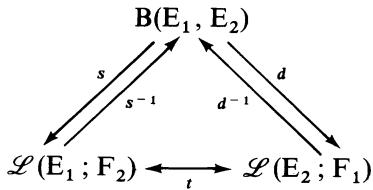
\includegraphics[keepaspectratio]{images/part001_08254dbd.jpg}}

其中 t 是转置同构（II, 第 46 页, 命题 5 及其推论）。鉴于 \(F_{1}\) 和 \(F_{2}\) 上弱拓扑的定义，立即可知：当给 \(\mathbf{B}(\mathbf{E}_{1}, \mathbf{E}_{2})\)、\(\mathcal{L}(\mathbf{E}_{1}; \mathbf{E}_{2})\) 和 \(\mathcal{L}(\mathbf{E}_{2}; \mathbf{F}_{1})\) 赋予简单收敛拓扑时，图 (3) 中的同构都是拓扑向量空间同构。

\subsection{Fréchet 空间乘积上的分别连续双线性映射}

命题 2. --- 设 E、F 和 G 是三个局部凸空间。假设 E 和 F 可度量化且 E 是桶型的。设 H 是从 E × F 到 G 中的分别连续双线性映射所成的一个集。假设对每个 x ∈ E，从 F 到 G 中的映射 u(x, .) 所成的集（u 取遍 H）是等度连续的。则 H 是等度连续的。

设 \(\mathrm{U}_n(\text{resp. } \mathrm{V}_n)\) 是 E（相应地，F）中 0 的邻域的一个基本序列。若 H 不等度连续，则存在 G 中 0 的一个闭的、凸的、均衡的邻域 W，使得对所有 \(n\)，\(\mathrm{H}(\mathrm{U}_n \times \mathrm{V}_n)\) 不含于 W。于是存在一个点对序列 \((x_n, y_n) \in \mathrm{U}_n \times \mathrm{V}_n\)，和 H 中元素的一个序列 \((u_n)\)，使得 \(u_n(x_n, y_n) \notin \mathrm{W}\)。设 \(p\) 是 W 的度规。对每个 \(y \in \mathrm{F}\) 和每个 \(u \in \mathrm{H}\)，从 E 到 G 中的映射 \(u(., y)\) 连续，因而 \(p \circ u(., y)\) 是 E 上的一个连续半范数。另一方面，对每个 \(x \in \mathrm{E}\)，映射 \(u(x, .)\)（对 \(u \in \mathrm{H}\)）所成的集是等度连续的；由于序列 \((y_n)\) 趋于 0，它是有界的，而所有 \(u(x, y_n)\)（对 \(n \geqslant 0\) 和 \(u \in \mathrm{H}\)）所成的集是有界的（III, 第 22 页, 命题 9）。由此可得，函数 \(p'(x) = \sup_{\substack{u \in \mathrm{H} \\ n \geqslant 0}} p(u(x, y_n))\) 是一个下半连续半

范数（有限的）于 E 上。由于 E 是桶型的，\(p'\) 连续（III, 第 24 页, 推论）。由于 \((x_{n})\) 在 E 中趋于 0，\(p'(x_{n})\) 趋于 0，故当 n 充分大时我们有 \(p'(x_{n}) \leqslant 1\)；但这时 \(p(u_{n}(x_{n}, y_{n})) \leqslant p'(x_{n}) \leqslant 1\)，因而 \(u_{n}(x_{n}, y_{n}) \in \mathbf{W}\)，这与关于 \(u_{n}, x_{n}, y_{n}\) 的假设矛盾。

推论 1. --- 设 E 和 F 是两个 Fréchet 空间，G 是一个局部凸空间。每个从 E × F 到 G 中的分别连续双线性映射都是连续的。

事实上，每个 Fréchet 空间都是桶型的（III, 第 25 页, 推论）。

设 E 和 F 是两个局部凸空间。我们用 \(\mathcal{B}(\mathrm{E},\mathrm{F})\) 记 \(E \times F\) 上的连续双线性型所成的空间，带上在形如 \(A \times B\) 的集上一致收敛的拓扑，其中 A（相应地，B）在 E（相应地，F）中有界。公式

\[
u (x, y) = \langle y, \phi (u) (x) \rangle
\]

（对 \(x \in \mathrm{E}\)、\(y \in \mathrm{F}\) 和 \(u \in \mathcal{B}(\mathrm{E}, \mathrm{F})\)）定义了一个连续线性单射 \(\phi\)，从 \(\mathcal{B}(\mathrm{E}, \mathrm{F})\) 到 \(\mathcal{L}_b(\mathrm{E}; \mathrm{F}_b')\) 中。

推论 2. --- 假设 E 和 F 可度量化且 E 是桶型的。则 \(\phi\) 是一个从 \(\mathcal{B}(\mathrm{E},\mathrm{F})\) 到 \(\mathcal{L}_b(\mathrm{E};\mathrm{F}_b')\) 上的拓扑向量空间同构。

设 \(f \in \mathcal{L}_b(\mathrm{E}; \mathrm{F}_b')\)。置 \(u(x, y) = \langle y, f(x) \rangle\)（对 \(x \in \mathrm{E}\) 和 \(y \in \mathrm{F}\)）。双线性型 \(u\)（在 \(\mathrm{E} \times \mathrm{F}\) 上的）是分别连续的；由命题 2，它属于 \(\mathcal{B}(\mathrm{E}, \mathrm{F})\)，且我们有 \(f = \phi(u)\)。因此 \(\phi\) 是一个从 \(\mathcal{B}(\mathrm{E}, \mathrm{F})\) 到 \(\mathcal{L}_b(\mathrm{E}; \mathrm{F}_b')\) 上的线性双射。立即可知 \(\phi\) 是双连续的，于是推论 2 得证。

\subsection{亚连续双线性映射}

在下面，我们将定义一个介于连续双线性映射的概念与分别连续双线性映射的概念之间的概念。

命题 3. --- 设 E、F、G 是三个局部凸空间，S 是 E 的有界子集的一个族。设 u 是从 E × F 到 G 中的一个分别连续双线性映射。下列性质等价：

\begin{enumerate}
\def\labelenumi{\alph{enumi})}
\item
  对 0 的每个邻域 \(\mathbf{W}\)（在 \(\mathbf{G}\) 中）和每个集 \(\mathbf{M} \in \mathfrak{S}\)，存在 0 的一个邻域 \(\mathbf{V}\)（在 \(\mathbf{F}\) 中），使得 \(u(\mathbf{M} \times \mathbf{V}) \subset \mathbf{W}\)。
\item
  对每个集 \(\mathbf{M} \in \mathfrak{S}\)，\(\mathbf{M}\) 在映射 \(x \mapsto u(x, .)\) 下的像是 \(\mathcal{L}(\mathrm{F}; \mathrm{G})\) 的一个等度连续子集。
\item
  映射 \(y \mapsto u(., y)\)（从 \(\mathbf{F}\) 到 \(\mathcal{L}_{\mathfrak{S}}(\mathbf{E}; \mathbf{G})\) 中）是连续的。
\item
  表明 \(y \mapsto u(., y)\) 在点 0 处连续，这是根据 \(\mathcal{L}_{\mathfrak{S}}(\mathrm{E}; \mathrm{G})\) 中 0 的邻域的定义（III, 第 13 页）；类似地，a) 表明 M 在映射 \(x \mapsto u(x, .)\) 下的像在点 0 处等度连续（III, 第 16 页）。
\end{enumerate}

定义 2. --- 设 u 是从 E × F 到 G 中的一个双线性映射。我们称 u 为 S-亚连续的，如果 u 分别连续且它满足命题 3 的等价条件 a)、b)、c) 之一。

命题 3 的条件 \(c)\) 表明，\(\mathfrak{S}\) -亚连续双线性映射的概念对 \(\mathfrak{S}\) 的依赖仅通过 \(\mathfrak{S}\) -拓扑（在 \(\mathcal{L}(\mathrm{E},\mathrm{G})\) 上的）实现。

对 F 的有界子集的每个集 T，我们类似地定义 T-亚连续映射的概念，只要在命题 3 中交换 E 与 F 的角色。称一个分别连续双线性映射 u 为 \((\mathfrak{S}, \mathfrak{T})\) -亚连续的，如果它既是 S-亚连续的又是 T-亚连续的。

每个从 \(E \times F\) 到 G 中的连续双线性映射对有界子集的集的每个对 \((\mathfrak{S}, \mathfrak{T})\) 都是 \((\mathfrak{S}, \mathfrak{T})\) -亚连续的：对 G 中 0 的每个邻域 W，存在 E 中 0 的一个邻域 U 和 F 中 0 的一个邻域 V，使得 \(u(U \times V) \subset W\)；由于每个集 \(M \in S\) 有界，存在 \(\lambda > 0\) 使得 \(\lambda M \subset V\)，于是

\[
u (\mathbf {M} \times \lambda \mathbf {V}) = u (\lambda \mathbf {M} \times \mathbf {V}) \subset u (\mathbf {U} \times \mathbf {V}) \subset \mathbf {W}.
\]

逆命题一般不成立（III, 第 47 页, 习题 3）。

命题 4. --- 设 u 是从 E × F 到 G 中的一个 S-亚连续双线性映射。对每个集 M ∈ S，u 在 M × F 上的限制是连续的，且对 F 的每个有界子集 Q，u(M × Q) 在 G 中有界。

第一个断言由 GT, X, § 2, No.~1 的推论 3 得出。设 W 是 G 中 0 的一个邻域；由假设，存在 F 中 0 的一个邻域 V，使得 \(u(\mathbf{M} \times \mathbf{V}) \subset \mathbf{W}\)。由于存在 \(\lambda \neq 0\) 使得 \(\lambda \mathbf{Q} \subset \mathbf{V}\)，我们有 \(\lambda u(\mathbf{M} \times \mathbf{Q}) = u(\mathbf{M} \times \lambda \mathbf{Q}) \subset \mathbf{W}\)，这就证明了命题的第二部分。

命题 5. --- 设 u 是从 E × F 到 G 中的一个 (S, T)-亚连续双线性映射。对每对集 M ∈ S、N ∈ T，u 在 M × N 上一致连续。命题由 GT, X, § 2, No.~1 的命题 2 和 GT, X, § 2, No.~2 的命题 5 立即得出。

命题 6. --- 若 F 是桶型空间，则每个从 E × F 到局部凸空间 G 中的分别连续双线性映射 u 对 E 的有界子集的每个集 S 都是 S-亚连续的。

换言之，线性映射 \(y \mapsto u(., y)\)（从 \(F\) 到 \(\mathcal{L}_b(E; G)\) 中）是连续的。只需（III, 第 30 页, 命题 3）证明：每个有界子集 \(M\)（\(E\) 的）在 \(x \mapsto u(x, .)\) 下的像在 \(\mathcal{L}(F; G)\) 中等度连续。但由命题 1（III, 第 28 页），这个像是 \(\mathcal{L}(F; G)\) 的一个简单有界子集，而由于 \(F\) 是桶型的，\(\mathcal{L}(F; G)\) 的每个简单有界子集都是等度连续的（III, 第 25 页, 定理 1）。

评注. --- 假设 F 的拓扑是 F 上使线性映射 \(h_{\alpha}:F_{\alpha}\to F\) 连续的最细局部凸拓扑（II, 第 27 页）。则命题 3 的条件 c)（III, 第 30 页）表明：若 E 和 G 是局部凸的，则双线性映射 \(u:E\times F\to G\) 是 S-亚连续的，当且仅当诸双线性映射

\[
(x, y _ {\alpha}) \mapsto u (x, h _ {\alpha} (y _ {\alpha}))
\]

（从 \(\mathbf{E} \times \mathbf{F}_{\alpha}\) 到 \(\mathbf{G}\) 中）中的每一个都是 \(\mathfrak{S}\) -亚连续的。

现在假设 \(\mathbf{E}\) 是一个局部凸空间，它是闭向量子空间的一个递增序列 \((\mathbf{E}_n)\)（\(\mathbf{E}\) 的）的严格归纳极限（II, 第 33 页）；则每个集 \(\mathbf{M} \in \mathfrak{S}\) 含于诸 \(\mathbf{E}_n\) 之一且在这个子空间中有界（III, 第 5 页, 命题 6）。我们用 \(\mathfrak{S}_n\) 记属于 \(\mathfrak{S}\) 且含于 \(\mathbf{E}_n\) 的所有子集所成的族。

命题 3 的条件 a)（III, 第 30 页）表明：为使双线性映射 \(u: \mathrm{E} \times \mathrm{F} \to \mathrm{G}\) 是 \(\mathfrak{S}\) -亚连续的，必要且充分的是诸限制 \(u_n: \mathrm{E}_n \times \mathrm{F} \to \mathrm{G}\)（\(u\) 的）中的每一个都是 \(\mathfrak{S}_n\) -亚连续的。

\subsection{亚连续双线性映射的扩张}

命题 7. --- 设 E、F、G 是三个局部凸空间，其中 G 假设为 Hausdorff 的；设 \(E_{0}\)（相应地，\(F_{0}\)）是 E（相应地，F）的一个稠密向量子空间。设 u 是从 \(E \times F\) 到 G 中的一个分别连续双线性映射。

\begin{enumerate}
\def\labelenumi{\arabic{enumi})}
\item
  若 \(u(\mathrm{E}_0 \times \mathrm{F}_0) = \{0\}\)，则 \(u = 0\)。
\item
  设 \(\mathfrak{S}_0\) 是 \(\mathbf{E}_0\) 的有界子集的一个族；若 \(u\) 在 \(\mathbf{E}_0 \times \mathbf{F}_0\) 上的限制是 \(\mathfrak{S}_0\) -亚连续的，则 \(u\) 本身也是。
\item
  由假设，对所有 \(x \in \mathrm{E}_0\)，连续线性映射 \(u(x, .)\) 在 \(\mathrm{F}_0\) 上为零，从而在 \(\mathrm{F}\) 上为零：因此对所有 \(y \in \mathrm{F}\)，连续线性映射 \(u(., y)\) 在 \(\mathrm{E}_0\) 上为零，从而在 \(\mathrm{E}\) 上为零。这就证明 \(u = 0\)。
\item
  对 G 中 0 的每个闭邻域 W 和每个集 \(\mathbf{M} \in \mathfrak{S}_0\)，由假设，存在 \(\mathrm{F}_0\) 中 0 的一个邻域 V，使得 \(u(\mathbf{M} \times \mathbf{V}) \subset \mathbf{W}\)。但 \(\overline{\mathbf{V}}\) 是 F 中 0 的一个邻域；对每个 \(x \in \mathbf{M}\)，关系 \(u(\{x\} \times \mathbf{V}) \subset \mathbf{W}\) 蕴含 \(u(\{x\} \times \overline{\mathbf{V}}) \subset \mathbf{W}\)，因为 \(u(x, .)\) 连续且 W 是闭的；因此 \(u(\mathbf{M} \times \overline{\mathbf{V}}) \subset \mathbf{W}\)，这就证明 \(u\) 是 \(\mathfrak{S}_0\) -亚连续的。
\end{enumerate}

命题 8. --- 设 E、F、G 是三个局部凸空间；假设 G 是 Hausdorff 且拟完备的。设 \(E_{0}\)（相应地，\(F_{0}\)）是 E（相应地，F）的一个稠密向量子空间，\(S_{0}\)（相应地，\(T_{0}\)）是 \(E_{0}\)（相应地，\(F_{0}\)）的有界子集的一个族，使得 E（相应地，F）的每个点都在 \(S_{0}\)（相应地，\(T_{0}\)）的某个元素的闭包中。则每个 \((\mathfrak{S}_{0}, \mathfrak{T}_{0})\) -亚连续双线性映射 u（从 \(E_{0} \times F_{0}\) 到 G 中的）都唯一地扩张为从 E × F 到 G 中的一个分别连续双线性映射 \(\overline{u}\)，且 \(\overline{u}\) 是 \((\mathfrak{S}_{0}, \mathfrak{T}_{0})\) -亚连续的。

\(\overline{u}\) 的唯一性和亚连续性由命题 7 得出；剩下要证明 \(\overline{u}\) 的存在性。对每个 \(y' \in F_{0}\)，连续线性映射 \(x' \mapsto u(x', y')\)（从 \(E_{0}\) 到 G 中的）唯一地扩张为一个连续线性映射 \(x \mapsto u_{1}(x, y')\)（从 E 到 G 中的）（III, 第 8 页, 命题 10）。立即由此可得，对每个 \(x \in E\)，映射 \(y' \mapsto u_{1}(x, y')\)（从 \(F_{0}\) 到 G 中的）是线性的；我们将证明它是连续的。由假设，存在 \(M \in S_{0}\)，使得 \(x \in M\)。对 G 中 0 的每个闭邻域 W，由假设，存在 \(F_{0}\) 中 0 的一个邻域 V，使得 \(u(M \times V) \subset W\)；由于 \(x \mapsto u_{1}(x, y')\) 连续，我们推出 \(u_{1}(\overline{\mathbf{M}} \times \mathbf{V}) \subset \mathbf{W}\)，特别地，\(u_{1}(x, y') \in \mathbf{W}\)（对所有 \(y' \in V\)）。这就确立了我们的断言。由命题 7，双线性映射 \(u_{1}\)（从 \(E \times F_{0}\) 到 G 中的）是 \((\mathfrak{S}_{0}, \mathfrak{T}_{0})\) -亚连续的。我们把证明结束于：在证明的第一部分中交换 E 与 F 的角色并应用于 \(u_{1}\)。
% semantic-fragments: legacy-input-seam
\relax{}
\subsection{\texorpdfstring{映射 \((u, v) \mapsto v \circ u\) 的亚连续性}{映射 (u, v) \textbackslash mapsto v \textbackslash circ u 的亚连续性}}

命题 9. --- 设 R、S、T 是三个 Hausdorff 局部凸空间。假设空间 \(\mathcal{L}(\mathbf{R};\mathbf{S})\) 、\(\mathcal{L}(\mathbf{S};\mathbf{T})\) 、\(\mathcal{L}(\mathbf{R};\mathbf{T})\) 分别赋予简单（相应地，紧、有界）收敛拓扑。则双线性映射 \((u, v) \mapsto v \circ u\) （从 \(\mathcal{L}(\mathrm{R}; \mathrm{S}) \times \mathcal{L}(\mathrm{S}; \mathrm{T})\) 到 \(\mathcal{L}(\mathrm{R}; \mathrm{T})\) 中）是 \((\mathfrak{S}, \mathfrak{T})\) -亚连续的，其中 \(\mathfrak{T}\) 是 \(\mathcal{L}(\mathrm{S}; \mathrm{T})\) 的等度连续子集所成的族，而 \(\mathfrak{S}\) 是 \(\mathcal{L}(\mathrm{R}; \mathrm{S})\) 的有限（相应地，紧、有界）子集所成的族。

我们先证明 \((u, v) \mapsto v \circ u\) 是 \(\mathfrak{T}\) -亚连续的。设 H 是 \(\mathcal{L}(S; T)\) 中的一个等度连续集，W 是 T 中 0 的一个邻域，M 是 R 的一个有限（相应地，紧、有界）子集。我们必须证明，存在 S 中 0 的一个邻域 V，使得若 \(u(M) \subset V\) 且 \(v \in H\) ，则 \(v(u(M)) \subset W\) 。但为此，只需 \(v(V) \subset W\) 对一切 \(v \in H\) 成立，而这样的邻域的存在性由 H 的等度连续性得出。

为了看出 \((u, v) \mapsto v \circ u\) 是 \(\mathfrak{S}\) -亚连续的，我们将证明：对 0 的每个邻域 \(W\) （在 \(T\) 中）、每个有限（相应地，紧、有界）子集 \(M\) （在 \(R\) 中）以及每个有限（相应地，紧、有界）子集 \(L\) （在 \(\mathcal{L}(R; S)\) 中），存在一个有限（相应地，紧、有界）子集 \(N\) （在 \(S\) 中） ，使得关系式 \(v(N) \subset W\) 与 \(u \in L\) 蕴含 \(v(u(M)) \subset W\) 。显然，只需证明可取 \(N = \bigcup_{u \in L} u(M)\) ，

即证明只要 L 与 M 是有限（相应地，紧、有界）的，集 N 就是有限（相应地，紧、有界）的。若 L 与 M 都是有限的，这立即可得；若 M 在 R 中有界且 L 在 \(\mathcal{L}(\mathrm{R};\mathrm{S})\) 中有界（对有界收敛拓扑，cf.~III, 第 22 页），这也立即可得。最后，我们证明：若 M 是 R 中的紧集，且 L 对紧收敛拓扑是 \(\mathcal{L}(\mathrm{R};\mathrm{S})\) 中的紧集，则 N 是 S 中的紧集。但若 \(u_{M}\) 是 \(u \in L\) 到 M 上的限制，则映射 \(u \mapsto u_{M}\) （从 L 到由 M 到 S 中的全体连续映射所成的空间 \(\mathcal{C}(\mathrm{M};\mathrm{S})\)（赋一致收敛拓扑）中）是连续的；因此 L 在此映射下的像是紧的，而我们的断言由映射 \((w,x) \mapsto w(x)\) （从 \(\mathcal{C}(\mathrm{M};\mathrm{S}) \times \mathrm{M}\) 到 S 中）的连续性得出（GT, X, § 1, No.~6, 命题 9）。

在下面两个推论中，我们同命题 9 一样假设：空间 \(\mathcal{L}(\mathbf{R};\mathbf{S})\) 、\(\mathcal{L}(\mathbf{S};\mathbf{T})\) 、\(\mathcal{L}(\mathbf{R};\mathbf{T})\) 三者都赋予简单收敛拓扑，或三者都赋予紧收敛拓扑，或三者都赋予有界收敛拓扑。

推论 1. --- 对 \(\mathcal{L}(\mathbf{S};\mathbf{T})\) 的每个等度连续子集 H，映射 \((u,v)\mapsto v\circ u\) （从 \(\mathcal{L}(\mathbf{R};\mathbf{S})\times \mathbf{H}\) 到 \(\mathcal{L}(\mathbf{R};\mathbf{T})\) 中）是连续的。

这由命题 9（III, 第 32 页）与命题 4（III, 第 31 页）立即得出。

推论 2. --- 假设 S 是桶型空间。若序列 \((u_n)\) 收敛于 \(u\) （在 \(\mathcal{L}(\mathbf{R};\mathbf{S})\) 中），且序列 \((v_{n})\) 收敛于 \(v\) （在 \(\mathcal{L}(\mathbf{S},\mathbf{T})\) 中），则序列 \((v_{n}\circ u_{n})\) 收敛于 \(v\circ u\) （在 \(\mathcal{L}(\mathbf{R};\mathbf{T})\) 中） 。

事实上，序列 \((v_{n})\) 在 \(\mathcal{L}(\mathrm{S};\mathrm{T})\) 中简单有界，由于 \(\mathrm{S}\) 是桶型空间（III, 第 25 页, 定理 1），它是等度连续的；于是该推论是推论 1 的结论。

\section{BOREL 图像定理}

\subsection{Borel 图像定理}

定理 1. --- 设 E 是一个作为 Banach 空间的归纳极限的局部凸空间，F 是一个 Souslin 局部凸空间，例如一个 Lusin 空间（GT, IX, § 6, No.~2 与 No.~4），u 是从 E 到 F 中的一个线性映射。若 u 的图像是 E × F 的一个 Borel 子集，则 u 连续。

设 \(E_i\) 是一族 Banach 空间，\((u_i)\) 是一族连续线性映射 \(u_i: E_i \to E\) ，使得 \(E\) 的拓扑是使诸 \(u_i\) 连续的最细局部凸拓扑。只需证明诸复合映射 \(u \circ u_i\) 都是连续的，或者事实上（GT, IX, § 2, No.~6, 命题 10）证明 \(u \circ u_i\) 到每个满足第一可数公理的闭子空间 \(G\) （在 \(E_i\) 中）上的限制都是连续的。这一限制的图像是 \(u\) 的图像在连续映射 \(u_i \times \text{Id}_F: G \times F \to E \times F\) 下的原像，因而是 \(G \times F\) 中的一个 Borel 集。此外，\(G \times F\) 是一个 Souslin 空间，而 Souslin 空间的每个 Borel 子集都是 Souslin 空间（GT, IX, § 6, No.~3, 命题 10）。于是定理 1 由 GT, IX, § 6, No.~8 的定理 4 得出。

注记. --- 回忆（III, 第 12 页），每个同调的 Hausdorff 半完备空间，例如每个 Fréchet 空间，都是 Banach 空间的归纳极限。* 这对自反 Fréchet 空间的强对偶也同样成立（IV, 第 23 页, 命题 4）。*

\subsection{局部凸 Lusin 空间}

命题 1. --- 设 E 是一个 Hausdorff 局部凸空间。假设存在一个由满足第一可数公理的 Fréchet 空间构成的序列 \((\mathrm{E}_{n})_{n\in\mathbb{N}}\) ，以及连续线性映射 \(u_{n}:E_{n}\to E\) ，使得 \(\mathrm{E}=\bigcup_{n\in\mathbb{N}}u_{n}(\mathrm{E}_{n})\) 。则 E 是一个 Lusin 空间。

设 \(P_n\) 是 \(u_n\) 的核；则 \(u_n\) 定义从商空间 \(E_n / P_n\) 到 \(u_n(E_n)\) 上的一个连续双射。由于 \(E_n / P_n\) 是满足第一可数公理的 Fréchet 空间（GT, IX, § 3, No.~1），从而是一个波兰空间（GT, IX, § 6, No.~1, 定义 1），故 \(u_n(E_n)\) 是 E 的一个 Lusin 子空间（GT, IX, § 6, No.~4, 命题 11）。于是由 GT, IX, § 6, No.~7, 定理 3 的推论，作为正则空间（GT, III, § 3, No.~1）的 E 是一个 Lusin 空间。

例 1. --- 每个满足第一可数公理的 Fréchet 空间都是一个波兰空间，从而是一个 Lusin 空间。因此，空间 \(\mathcal{C}(\mathrm{X})\) （其中 \(\mathrm{X}\) 局部紧且具有可数基）亦然（\(\mathcal{C}(\mathrm{X})\) 的拓扑取为紧收敛拓扑，cf.~GT, X, § 3, No.~3, 推论 与 § 1, No.~6, 推论 3）；* 空间 \(\mathcal{C}^{\infty}(\mathrm{U})\) （其中 U 是 \(\mathbf{R}^{n}\) 的开子集（III, 第 9 页））与空间 \(\mathcal{H}(\mathrm{U})\) （其中 U 是 \(\mathbf{C}^{n}\) 的开子集（III, 第 10 页））也都如此。

命题 1 表明，空间 \(\mathcal{C}_0^\infty (\mathbf{U})\) （其中 \(\mathbf{U}\) 是 \(\mathbf{R}^n\) 中的开集）、\(\mathcal{G}_s(\mathbf{I})\) （其中 \(\mathbf{I}\) 是 \(\mathbf{R}\) 中的紧区间且 \(s\geqslant 1\) ）以及 \(\mathcal{H}(\mathbf{K})\) （其中 \(\mathbf{K}\) 是 \(\mathbf{C}^n\) 的紧子集）都是 Lusin 空间（III, 第 10 页）。

定理 2. --- 设 E 是一个局部凸空间，它是 E 的子空间所成的递增序列 \((\mathrm{E}_n)_{n\in \mathbb{N}}\) 的归纳极限，诸子空间赋予满足第一可数公理的 Fréchet 空间拓扑。假设 E 的每个紧子集都含于某个 \(E_{n}\) 之中，且在这个空间中是紧的。设 F 是满足第一可数公理的 Fréchet 空间。则空间 \(\mathcal{L}_{c}(E;F)\) 是一个 Lusin 空间。

空间 E 是有界型空间（III, 第 12 页），因此空间 \(\mathcal{L}_c(\mathrm{E};\mathrm{F})\) 是完备的（III, 第 23 页, 命题 12）。线性映射 \(j\colon f\mapsto (f|\mathrm{E}_n)_{n\in \mathbf{N}}\) 是从 \(\mathcal{L}_c(\mathrm{E};\mathrm{F})\) 到乘积空间 \(\prod_{n\in \mathbf{N}}\mathcal{L}_c(\mathrm{E}_n;\mathrm{F})\) 中的一个单射；凭借关于 E 的紧子集的假设以及诸 \(\mathfrak{S}\) -拓扑的定义，\(j\) 是从 \(\mathcal{L}_c(\mathrm{E};\mathrm{F})\) 到它的像上（该像赋予由乘积拓扑诱导的拓扑）的一个同构；此外，由于 \(\mathcal{L}_c(\mathrm{E};\mathrm{F})\) 完备，这个像是 \(\prod_{n\in \mathbf{N}}\mathcal{L}_c(\mathrm{E}_n;\mathrm{F})\) 的一个闭子空间

（GT, II, § 3, No.~4, 命题 8）。于是由 GT, IX, § 6, No.~4，只需证明诸空间 \(\mathcal{L}_c(\mathrm{E};\mathrm{F})\) 中的每一个都是 Lusin 空间。在证明的其余部分，我们将假设 E 是满足第一可数公理的 Fréchet 空间。

由于 F 是满足第一可数公理的 Fréchet 空间，它同构于 Banach 空间的一个可数乘积的闭子空间，其中每个 Banach 空间 \(F_{n}\) 都是 F 的商（II, 第 5 页），因而满足第一可数公理。线性映射 \(j': f \mapsto (\mathrm{pr}_{n} \circ f)_{n \in \mathbb{N}}\) 是从 \(\mathcal{L}_{c}(\mathrm{E}; \mathrm{F})\) 到乘积空间 \(\prod_{n \in \mathbb{N}} \mathcal{L}_{c}(\mathrm{E}; \mathrm{F}_{n})\) 中的一个单射，并且利用诸 S-拓扑以及乘积中开集的定义，\(j'\) 是从 \(\mathcal{L}_{c}(\mathrm{E}; \mathrm{F})\) 到它的像上的一个同构；此外，由于 \(\mathcal{L}_{c}(\mathrm{E}; \mathrm{F})\) 完备，这个像是 \(\prod_{n \in \mathbb{N}} \mathcal{L}_{c}(\mathrm{E}; \mathrm{F})\) 的一个闭子空间。因此只需证明诸空间 \(\mathcal{L}_{c}(\mathrm{E}; \mathrm{F}_{n})\) 中的每一个都是 Lusin 空间（GT, IX, § 6, No.~4），从而我们可以假设 F 是满足第一可数公理的 Banach 空间。

空间 \(\mathcal{L}_{c}(\mathrm{E};\mathrm{F})\) 是等度连续闭子集所成可数族的并（III, 第 19 页, 推论 1 与 GT, X, § 2, No.~3, 命题 6）。但 \(\mathcal{L}_{c}(\mathrm{E};\mathrm{F})\) 的每个等度连续子集 H 都是可度量化的且满足第一可数公理（III, 第 18 页, 命题 6 与 GT, X, § 2, No.~4, 定理 1）；若 H 是闭的，则它对由 \(\mathcal{L}_{c}(\mathrm{E};\mathrm{F})\) 的一致结构诱导的一致结构而言是完备的空间，因为后者是完备的。换言之，H 是一个波兰空间，从而更是 Lusin 空间；于是正则空间 \(\mathcal{L}_{c}(\mathrm{E};\mathrm{F})\) 是一个 Lusin 空间（GT, IX, § 6, No.~7, 定理 3 的推论）。

推论. --- 在关于 E 的假设与定理 2 相同的前提下，再假设 E 的每个有界子集都是相对紧的。则 E 的强对偶是一个 Lusin 空间。* 特别地，满足第一可数公理的 Fréchet 空间若同时是 Montel 空间，则其强对偶是 Lusin 空间。*

* 例 2. --- 设 U 是 \(\mathbf{R}^{n}\) 的一个开子集。上述推论特别适用于 Fréchet 空间 \(E = \mathcal{C}^{\infty}(\mathrm{U})\) ；它的对偶 \(\mathcal{C}_{0}^{-\infty}(\mathrm{U})\) （U 上具有紧支集的广义函数所成的空间）于是是一个 Lusin 空间。空间 \(\mathcal{C}_{0}^{\infty}(\mathrm{U})\) 是满足第一可数公理的一列 Fréchet 空间 \(\mathcal{C}_{K_n}^{\infty}(\mathrm{U})\) 的严格归纳极限（III, 第 9 页）。我们可以证明，诸空间 \(\mathcal{C}_{K_n}^{\infty}(\mathrm{U})\) 中的每一个都是 Montel 空间；此外，\(\mathcal{C}_{0}^{\infty}(\mathrm{U})\) 的每个有界子集都含于诸空间 \(\mathcal{C}_{K_n}^{\infty}(\mathrm{U})\) 之一（III, 第 5 页, 命题 6）。于是可以应用定理 2 的推论。从而 \(\mathcal{C}_{0}^{-\infty}(\mathrm{U})\) （\(\mathcal{C}_{0}^{\infty}(\mathrm{U})\) 的对偶，U 上的广义函数空间）对强拓扑而言是一个 Lusin 空间。*

类似地可以证明：对 \(C^{n}\) 的每个开子集 U 以及 \(C^{n}\) 的每个紧子集 K，\(\mathcal{H}(U)\) 的强对偶与 \(\mathcal{H}(K)\) 的强对偶都是 Lusin 空间。*

注记. --- 设 E 如定理 2 中所示；设 F 是一个 Hausdorff 局部凸空间，它是一列连续线性映射 \(u_n: \mathrm{F}_n \to \mathrm{F}\) 的像的并，其中每个 \(\mathrm{F}_n\) 都是满足第一可数公理的 Fréchet 空间；则 \(\mathcal{L}_c(\mathrm{E};\mathrm{F})\) 是一个 Lusin 空间。如命题 1 中那样，我们先化归到每个 \(u_n\) 都是单射的情形；然后，如定理 2 的证明中那样，可以假设 E 是满足第一可数公理的 Fréchet 空间。于是由 I, 第 20 页, 命题 1，\(\mathcal{L}(\mathrm{E};\mathrm{F})\) 是诸 \(\mathcal{L}(\mathrm{E};\mathrm{F}_n)\) 的并；此外，典范单射 \(\mathcal{L}_c(\mathrm{E};\mathrm{F}_n) \to \mathcal{L}_c(\mathrm{E};\mathrm{F})\) 连续（GT, X, § 1, No.~4, 命题 3）。由于由定理 2，诸空间 \(\mathcal{L}_c(\mathrm{E};\mathrm{F}_n)\) 中的每一个都是 Lusin 空间，故 \(\mathcal{L}(\mathrm{E};\mathrm{F}_n)\) 对由 \(\mathcal{L}_c(\mathrm{E};\mathrm{F})\) 的拓扑诱导的拓扑而言也是 Lusin 空间（GT, IX, § 6, No.~4, 命题 11）；于是由 GT, IX, § 6, No.~7, 定理 3 的推论，\(\mathcal{L}_c(\mathrm{E};\mathrm{F})\) 是一个 Lusin 空间。

\subsection{\texorpdfstring{* Banach 空间上的可测线性映射 \(^{1}\)}{Banach 空间上的可测线性映射 \^{}\{1\}}}

命题 2. --- 设 E 是一个 Banach 空间，F 是一个局部凸空间，u 是从 E 到 F 中的一个线性映射。假设对 F 的每个闭子集 B、E 的每个紧子集 X 以及 X 上的每个测度 \(\mu\) ，交集 \(X \cap u^{-1}(B)\) 都是 \(\mu\) -可测的。则 u 连续。

先假设 F 是基域。对 E 的每个紧子集 X 以及 X 上的每个测度 \(\mu\) ，u 到 X 上的限制是 \(\mu\) -可测的（INT, IV）。假设 u 不连续。则可以找到 E 中的点列 \((x_{n})\) ，使得 \(\sum_{n} \|x_{n}\| < \infty\) 且对每个整数 n 有 \(|u(x_{n})| \geqslant n\) 。考虑映射 \(g:(t_{n}) \mapsto \sum_{n} t_{n} x_{n}\) （从立方体 \(C = [0, 1]^{N}\) 到 E 中）；显然 g 连续。因此 \(f = u \circ g\) 对 C 上的每个测度都可测（INT, V）；特别地，对作为 C 的诸因子上 Lebesgue 测度的乘积的测度 \(\mu\) 可测。于是存在 C 的一个紧子集 D，使得 \(\mu(D) > \frac{1}{2}\) ，且 f 在 D 上的限制连续，从而也有界。设 M 是 \(|f|\) 在 D 上的上确界，设 \(p \in N\) 使得 \(p \geqslant 4M\) 。设 \(s = (s_{n})\) 与 \(t = (t_{n})\) 是 D 中满足 \(s_{n} = t_{n}\) （对一切 \(n \neq p\) ）的两个点。则

\[
f (s) - f (t) = u (\sum_ {n} s _ {n} x _ {n} - \sum_ {n} t _ {n} x _ {n}) = (s _ {p} - t _ {p}) u (x _ {p}).
\]

由于 \(|f(s) - f(t)| \leqslant 2\mathbf{M}\) 且 \(|u(x_p)| \geqslant p \leqslant 4\mathbf{M}\) ，我们得到

\[
\left| s _ {p} - t _ {p} \right| \leqslant \frac {1}{2}.
\]

Lebesgue-Fubini 定理（INT, V, 第 2 版, § 8, No.~3, 命题 7 的推论 2）蕴含 \(\mu(D) \leqslant \frac{1}{2}\) ；这就导出矛盾。因此 \(u\) 连续。

在一般情形，对每个 \(v \in F'\) ，线性型 \(v \circ u\) 由前面的论证是连续的。设 \((x_{n})_{n \in \mathbb{N}}\) 是 E 中收敛于 0 的点列；则序列 \((u(x_{n}))_{n \in \mathbb{N}}\) 在 F 中收敛于 0（当 F 赋予拓扑 \(\sigma(\mathrm{F}, \mathrm{F}')\) 时）；因此这个序列对 \(\sigma(\mathrm{F}, \mathrm{F}')\) 有界，从而在 F 中有界（III, 第 27 页, 推论 3）。由于 E 是有界型空间（III, 第 12 页, 命题 2），线性映射 \(u: E \to F\) 连续。*

1 本节的结果依赖于积分（Integration）一书。

\exercisesheading
\exercisegroup

\begin{enumerate}
\def\labelenumi{\arabic{enumi})}
\tightlist
\item
  设 \(\mathbf{E}\) 是非离散拓扑域 \(\mathbf{K}\) 上的一个左拓扑向量空间。称 \(\mathbf{B}\) （\(\mathbf{E}\) 的子集）是有界的，如果对 0 的每个邻域 \(\mathbf{V}\) （\(\mathbf{E}\) 中），存在 \(\lambda \neq 0\) （\(\mathbf{K}\) 中），使得 \(\lambda \mathbf{B} \subset \mathbf{V}\) 。
\end{enumerate}

\begin{enumerate}
\def\labelenumi{\alph{enumi})}
\item
  证明：若 B 在 E 中有界，则对 E 中 0 的每个邻域 V，存在 K 中 0 的一个邻域 U，使得 U.B ⊂ V。
\item
  证明：E 中有界集的闭包是有界的。两个有界集的并是有界的。E 中每个预紧集都是有界的。把 III, 第 4 页, 命题 4 的诸推论推广到 K 上的拓扑向量空间。
\item
  证明：若 A 是 K 中的有界集（把 K 视为自身上的左向量空间），B 是 E 中的有界集，则 A.B 在 E 中有界。
\item
  把 III, 第 4 页 的命题 3 推广到 K 是可度量化拓扑除环的情形。e) 把拟完备空间的概念及其性质推广到拓扑向量空间。
\end{enumerate}

\begin{enumerate}
\def\labelenumi{\arabic{enumi})}
\setcounter{enumi}{1}
\tightlist
\item
  \begin{enumerate}
  \def\labelenumii{\alph{enumii})}
  \tightlist
  \item
    设 E 是非离散拓扑域 K 上的一个左拓扑向量空间。证明：若存在 E 中 0 的一个有界邻域 V（习题 1），则诸集 \(\lambda\) V（\(\lambda \in \mathbf{K}\) 且 \(\lambda \neq 0\) ）构成 E 中 0 的一个基本邻域系。若 K 可度量化，则与 E 的拓扑相伴的 Hausdorff 拓扑（GT, III, § 2, No.~6）可度量化。若 \(\mathbf{K} = \mathbf{R}\) 或 \(\mathbf{K} = \mathbf{C}\) ，则 E 上比 E 的给定拓扑更粗的诸拓扑之中的最细局部凸拓扑（II, 第 80 页, 习题 23）可由单个半范数定义。
  \end{enumerate}
\end{enumerate}

\begin{enumerate}
\def\labelenumi{\alph{enumi})}
\setcounter{enumi}{1}
\item
  证明：局部凸 Hausdorff 空间（其中没有一个仅是点 0）的无穷乘积的拓扑不能由单个半范数定义。
\item
  设 E 是一个局部凸空间，其拓扑由半范数的递增序列 \((p_n)\) 定义。要使 E 的拓扑可由单个半范数定义，必须且只需存在整数 \(n_0\) ，使得对每个 \(n \geqslant n_0\) ，存在数 \(k_n \geqslant 0\) ，使得 \(p_n(x) \leqslant k_n p_{n_0}(x)\) 对一切 \(x \in E\) 成立。
\end{enumerate}

\(d\) ) 设 E 是 \(\mathbf{R}\) 上的向量空间，由区间 \(\mathrm{I} = [0,1]\) 上无穷可微的数值函数组成。对每个整数 \(n\geqslant 0\) ，令 \(p_n(f) = \sup_{0\leqslant k\leqslant n}\left(\sup_{x\in I}|f^{(k)}(x)|\right)\) （其中

\(f^{(0)} = f)\) ）；证明诸 \(p_n\) 是 E 上的范数，且由范数序列 \(p_n\) 定义的拓扑不能由单个范数定义。

\begin{enumerate}
\def\labelenumi{\arabic{enumi})}
\setcounter{enumi}{2}
\item
  设 E 是 R 上的可度量化向量空间，d 是与 E 的拓扑相容的平移不变距离。令 \(|x| = d(x, 0)\) （I, 第 16 页）。证明：对每个整数 n \textgreater{} 0，有 \(\frac{1}{n}|x| \leqslant \left|\frac{x}{n}\right|\) 。由此推出：若 B 是 E 的有界子集，则 \(\sup_{x \in B} |x| < +\infty\) （换言之，B 对距离 d 有界（GT, IX, § 2, No.~3））。给出一个可度量化向量空间 E 以及 E 中一个集合的例子，该集合无界但对距离 d 有界（习题 2）。
\item
  设 E 是非离散可度量化拓扑域 K 上的一个拓扑向量空间。证明：若 E 是 Baire 空间，且 E 中由有界子集构成的有界结构具有可数基（III, 第 37 页, 习题 1），则存在 E 中 0 的一个有界邻域，从而与 E 的拓扑相伴的 Hausdorff 拓扑可度量化（III, 第 37 页, 习题 2）（与习题 6 比较）。
\item
  设 \(\mathbf{E}\) 是非离散赋值域 \(\mathbf{K}\) 上的可度量化向量空间。证明：若 \((\mathbf{B}_n)\) 是 \(\mathbf{E}\) 的有界子集的任意一个序列（III, 第 37 页, 习题 1），则存在标量的一个序列 \((\lambda_n)\) （诸标量 \(\neq 0\)），使得诸集 \(\lambda_n\mathbf{B}_n\) 的并是有界的。
\item
  设 \(\mathrm{E}\) 是一个局部凸空间，它是局部凸 Hausdorff 空间的严格递增序列 \((\mathrm{E}_n)\) 的严格归纳极限，且每个 \(\mathrm{E}_n\) 在 \(\mathrm{E}_{n+1}\) 中闭（II, 第 32 页, 命题 9）。
\end{enumerate}

\begin{enumerate}
\def\labelenumi{\alph{enumi})}
\tightlist
\item
  证明 E 不可度量化（利用 III, 第 5 页, 命题 6 以及前面的习题 5）。\\
\item
  要使 E 的典范有界结构具有可数基，必须且只需每个 \(\mathrm{E}_n\) 的典范有界结构在 \(\mathrm{E}_n\) 中具有可数基。
\end{enumerate}

\begin{enumerate}
\def\labelenumi{\arabic{enumi})}
\setcounter{enumi}{6}
\tightlist
\item
  \begin{enumerate}
  \def\labelenumii{\alph{enumii})}
  \tightlist
  \item
    设 E 是一个无穷维 Banach 空间，S 是 E 的紧凸均衡子集所成的族，它对关系 \(\subset\) 是有向集。证明：E 是 Banach 空间 \(E_{A}\) （A 取遍 S）的归纳系统的归纳极限。（用反证法证明：对诸 \(E_{A}\) 的拓扑的归纳极限拓扑而言，0 的邻域 V 含有一个以 0 为中心的球；为此，注意否则将存在 E 中的点列 \((x_{n})\) ，使得 \(\|x_{n}\| \leqslant 1/n^{2}\) ，且不属于 V。）由此推出：E 中存在不含于任何 \(E_{A}\) （\(A \subset S\) ）的有界子集。
  \end{enumerate}
\end{enumerate}

\begin{enumerate}
\def\labelenumi{\alph{enumi})}
\setcounter{enumi}{1}
\tightlist
\item
  设 E 是一个无穷维 Banach 空间。在向量空间 \(\prod_{m=1}^{\infty}E_{m}\) （其中对每个 m 有 \(E_{m}=E\) ）上，用 \(T_{n}\) 表示这样的拓扑：在每个 \(E_{m}\) （\(m\leqslant n\) ）上取 Banach 空间拓扑的乘积，而对 m\textgreater n 取 \(E_{m}\) 上的最细局部凸拓扑；用 \(F_{n}\) 表示局部凸空间 \(\prod_{m=1}^{\infty}E_{m}\) （赋以拓扑 \(T_{n}\) ）。每个恒等映射 \(F_{n}\to F_{n+1}\) 都连续；证明：归纳系统 \(F_{n}\) 的归纳极限空间是空间 F，其中 F 是在 \(\prod_{m=1}^{\infty}E_{m}\) 上赋以各因子的 Banach 空间拓扑之乘积而得到的空间。由此推出：F 中存在在任何 \(F_{n}\) 中都无界的有界子集。
\end{enumerate}

\begin{enumerate}
\def\labelenumi{\arabic{enumi})}
\setcounter{enumi}{7}
\item
  证明：在一个由拓扑向量空间（在 \(\mathbf{R}\) 或 \(\mathbf{C}\) 上，没有一个仅是点 0）作成的无穷乘积的空间中，典范有界结构不具有可数基（首先证明只需对空间 \(\mathbf{R}^{\mathbf{N}}\) 证明这一点，然后利用 III, 第 38 页, 习题 4）。
\item
  设 E 是 R 上由区间 I = \{0, 1\} 上全体调节函数（FVR, I, 第 4 页）组成的向量空间。对每个整数 n \textgreater{} 0，令 \(V_{n}\) 为全体函数 \(f \in E\) （满足 \(\int_{0}^{1} \sqrt{|f(t)|} dt \leqslant 1/n\) ）所成的集。证明：诸集 \(V_{n}\) 构成 E 上一个与 E 的向量空间结构相容的可度量化拓扑的 0 的基本邻域系，且对该拓扑诸集 \(V_{n}\) 是有界的；但每个 \(V_{n}\) 的凸包是整个空间 E。（注意每个函数 \(f \in E\) 都可写成 \(f = \frac{1}{2}(g + h)\) ，其中 g 与 h 属于 E，且
\end{enumerate}

\[
\int_ {0} ^ {1} \sqrt {| g (t) |} d t = \int_ {0} ^ {1} \sqrt {| h (t) |} d t = \frac {1}{\sqrt {2}} \int_ {0} ^ {1} \sqrt {| f (t) |} d t.
\]

由此推出：E 上比 E 的拓扑更粗的唯一的局部凸拓扑是 E 上的最粗拓扑。

\begin{enumerate}
\def\labelenumi{\arabic{enumi})}
\setcounter{enumi}{9}
\tightlist
\item
  设 \((\mathrm{E}_{\iota})_{\iota \in I}\) 是非离散拓扑域 K 上由 Hausdorff 拓扑向量空间组成的一个无穷族，其中没有一个仅是点 0。设 E 是诸 \(\mathbf{E}_{\iota}\) 的直和向量空间，\(\mathcal{T}_0\) 是 I, 第 24 页, 习题 14 中定义的 E 上的拓扑。那么，E 的子集 B 对 \(\mathcal{T}_0\) 有界（III, 第 37 页, 习题 1），当且仅当 B 含于某个乘积子空间 \(\prod_{\iota \in H} \mathbf{E}_{\iota}\) ，其中 H 是 I 的一个有限
\end{enumerate}

子集，且 B 在每个 \(E_{\iota}\) （\(\iota \in H\) ）上的投影是有界的。由此推出（对 K = R 或 C）：若每个 \(E_{\iota}\) 都是拟完备空间，则赋以 \(T_{0}\) 的 E 是拟完备的。

\begin{enumerate}
\def\labelenumi{\arabic{enumi})}
\setcounter{enumi}{10}
\tightlist
\item
  设 \(\mathbf{E}\) 是带非离散赋值的域 \(\mathbf{K}\) 上的一个拓扑向量空间。
\end{enumerate}

\begin{enumerate}
\def\labelenumi{\alph{enumi})}
\item
  为使 E 的均衡子集 A 吸收 E 的每个有界子集（III, 第 37 页, 习题 1），只需 A 吸收 E 中每个趋于 0 的序列 \((x_{n})\) 的点所成的集即可。此时称 A 是吸有界集的。
\item
  设 \(u\) 是从 \(E\) 到一个拓扑向量空间 \(F\) （\(K\) 上的）中的线性映射。\(E\) 的每个有界子集在 \(u\) 下的像在 \(F\) 中有界，当且仅当对每个点列 \((x_{n})\) （\(E\) 中的、趋于 0 的），序列 \((u(x_{n}))\) 在 \(F\) 中有界。
\item
  假设 \(\mathbf{E}\) 可度量化。证明：\(\mathbf{E}\) 的每个吸有界集的子集都是 \(\mathbf{E}\) 中 0 的一个邻域。由此推出：若 \(u\) 是从 \(\mathbf{E}\) 到一个拓扑向量空间 \(\mathbf{F}\) （\(\mathbf{K}\) 上的）中的线性映射，它把 \(\mathbf{E}\) 中每个收敛于 0 的序列变为 \(\mathbf{F}\) 中的有界序列，则 \(u\) 在 \(\mathbf{E}\) 上连续。
\end{enumerate}

\begin{enumerate}
\def\labelenumi{\arabic{enumi})}
\setcounter{enumi}{11}
\item
  设 E 是带非离散赋值的域 K 上的 Hausdorff 拓扑向量空间，F 是 K 上的可度量化向量空间。若 u 是从 E 到 F 中的连续线性映射，使得对 F 的每个有界子集 B，\(u^{-1}(\mathbf{B})\) 在 E 中有界，证明 u 是从 E 到 F 的一个子空间上的同构。
\item
  设 \(I\) 是无穷集，\((E_{\iota})_{\iota\in I}\) 是一族局部凸空间，其中没有一个是 0。设 \(f\) 是从 \(E = \prod_{\iota\in I}E_{\iota}\) 到 Banach 空间 \(F\) 中的一个线性映射。证明：若 E 的每个有界子集在 f 下的像都是 F 的有界子集，则存在 I 的有限子集 H，使得对每个 \(\iota \notin H\) ，f 在 \(E_{\iota}\) （视为 E 的子空间）上的限制是零。（用反证法：否则可以构造 E 中的有界序列 \((x_{n})\) ，使其在 f 下的像在 F 中无界。）
\item
  证明：若可度量化局部凸空间 E 的拓扑不能由单个范数定义，则 E 的典范有界结构不存在可数基（利用 III, 第 38 页, 习题 5，证明否则 E 中将存在一个有界的吸有界集的集合（III, 第 39 页, 习题 11），并利用 III, 第 39 页, 习题 11, c) 完成论证）。
\item
  在 R 上的 Hausdorff 拓扑向量空间 E 中，设 A 是紧凸集，B 是闭的凸有界集。证明：并 \(A \cup B\) 的凸包 C 是闭集。（考虑 C 的闭包中不属于 A 的一点 z，并化归到 z = 0 的情形。注意存在 0 的一个邻域 V 和一个数 \(\alpha < 1\) ，使得关系式 \(0 \leqslant \lambda \leqslant 1\) 、\(x \in A\) 、\(y \in B\) 、\(\lambda x + (1 - \lambda)y \in V\) 蕴含 \(\lambda \leqslant \alpha\) 。然后，对 0 的每个邻域 W，考虑三元组 \((\lambda, x, y)\) （满足 \(\lambda x + (1 - \lambda)y \in W\) 、\(0 \leqslant \lambda \leqslant 1\) 、\(x \in A\) 、\(y \in B\) ）全体所成的集。）
\item
  设 \(\mathbf{E}\) 是满足第一可数公理的可度量化局部凸空间，且其完备化 \(\hat{\mathbf{E}}\) 是满足第一可数公理的 Fréchet 空间。
\end{enumerate}

证明：\(\hat{E}\) 的每个有界子集 B 都含于 \(\hat{E}\) 的某个有界子集的闭包中。（化归到 B 可数、并排成序列 \((x_{n})\) 的情形；另一方面，设 \((p_{n})\) 是定义 \(\hat{E}\) 的拓扑的半范数的递增序列；对每个整数 n，考虑 E 的点列 \((y_{nk})_{k\geqslant1}\) ，它收敛于 \(x_{n}\) ，且满足 \(p_{n}(x_{n}-y_{nk})\leqslant1\) （对一切 \(k\geqslant1\)）。）

\begin{enumerate}
\def\labelenumi{\arabic{enumi})}
\setcounter{enumi}{16}
\tightlist
\item
  设 \(\mathbf{A}\) 是 \(\geqslant 1\) 的、从 \(\mathbf{N}\) 到 \(\mathbf{N}\) 中的递增映射全体所成的集；对每个 \(\alpha \in \mathbf{A}\) ，用 \(\mathbf{B}_{\alpha}\) 表示由所有点 \(z = (z_n) \in \mathbf{R}^{\mathbf{N}}\) （它们满足 \(|z_n| \leqslant \alpha(n)\) ，对一切 \(n \in \mathbf{N}\) ）组成的集。
\end{enumerate}

\begin{enumerate}
\def\labelenumi{\alph{enumi})}
\item
  证明：诸集 \(\mathbf{B}_{\alpha}\) 构成空间 \(\mathbf{R}^{\mathbf{N}}\) 的全体有界子集所成的有界结构的一个基。b) 对每个 \(\alpha \in \mathbf{A}\) ，集 \(\mathbf{RB}_{\alpha}\) 是 \(\mathbf{R}^{\mathbf{N}}\) 的向量子空间，它异于 \(\mathbf{R}^{\mathbf{N}}\) 且在 \(\mathbf{R}^{\mathbf{N}}\) 中稠密；因此存在一个线性型 \(f_{\alpha} \neq 0\) （不连续的，在 \(\mathbf{R}^{\mathbf{N}}\) 上），使得 \(f_{\alpha}(z) = 0\) 对一切 \(z \in \mathbf{B}_{\alpha}\) 成立。
\item
  设 \(\mathbf{E}\) 是由所有映射 \(g: \alpha \mapsto (g_n(\alpha)) \in \mathbf{R}^{\mathbf{N}}\) （从 \(\mathbf{A}\) 到 \(\mathbf{R}^{\mathbf{N}}\) 中，且对一切 \(n \in \mathbf{N}\) 使和 \(p_n(g) = \sum_{\alpha} |g_n(\alpha)|\) 为有限）全体所成的向量空间。证明诸 \(p_n\) 是半范数
\end{enumerate}

它们在 E 上定义出一个 Fréchet 空间的拓扑。

\(d\) ) 设 \(\mathbf{H}\) 是由所有 \(h\in \mathbf{E}\) （满足 \(h(\alpha)\in \mathbf{RB}_2\) ，对一切 \(\alpha \in \mathbf{A}\)）组成的集；证明 \(\mathbf{H}\) 是 \(\mathbf{E}\) 的一个处处稠密的向量子空间（注意：若 \(h\in \mathbf{E}\) 满足 \(h(\alpha) = 0\) （除 \(\alpha \in \mathbf{A}\) 的有限多个值外），则它属于 \(\mathbf{H}\) ）。

\begin{enumerate}
\def\labelenumi{\alph{enumi})}
\setcounter{enumi}{4}
\tightlist
\item
  设 \(\mathrm{E}_0 \subset \mathrm{E}\) 是 \(\mathrm{E}\) 中由所有 \(g \in \mathrm{E}\) （满足 \(\sum_{\alpha} |f_{\alpha}(g(\alpha))| < +\infty\) ）组成的向量子空间；
\end{enumerate}

此时映射 \(u: g \mapsto (f_{\alpha}(g(\alpha)))_{\alpha \in \mathbf{A}}\) 是从 \(\mathrm{E}_0\) 到 Banach 空间 \(\mathrm{F} = \ell^1(\mathrm{A})\) 中的一个线性映射（I, 第 4 页）。证明 \(u(\mathrm{E}_0)\) 在 \(\mathrm{F}\) 中处处稠密（注意对每个有限子集 \(\mathrm{J}\) （\(\mathrm{A}\) 的），存在 \(g \in \mathrm{E}_0\) ，使得 \(g(\alpha) = 0\) （对一切 \(\alpha \in \mathrm{A} - \mathrm{J}\)），且诸 \(f_{\alpha}(g(\alpha))\) （对 \(\alpha \in \mathrm{J}\)）取 \(\mathbf{R}\) 中任意值）。证明 \(u^{-1}(0)\) 在 \(\mathrm{E}_0\) 中处处稠密（利用 \(d\) ）。最后证明：对每个有界子集 \(C\) （\(E\) 的），存在 \(\alpha_0 \in A\) ，使得 \(f_{\alpha_0}(g(\alpha_0)) = 0\) 对一切 \(g \in C \cap E_0\) 成立，并由此推出 \(u(C \cap E_0)\) 在 \(F\) 中的闭包不是 \(F\) 中 0 的邻域。

\begin{enumerate}
\def\labelenumi{\alph{enumi})}
\setcounter{enumi}{5}
\tightlist
\item
  设 G 是 u 在 \(E_{0} \times F\) 中的图像，它是 Fréchet 空间 \(E \times F\) 的一个向量子空间。证明 G 在 \(E \times F\) 中处处稠密（注意对每个 \(x \in E_{0}\) ，\(x + u^{-1}(0)\) 在 E 中稠密）。然而证明：对 G 的每个有界子集 M，闭包 \(\overline{M}\) （M 在 \(E \times F\) 中的）不包含有界集 \(\{0\} \times U\) （\(E \times F\) 中的），其中 U 是 F 中的单位球（若 \(N = \text{pr}_{1}(M)\) ，注意由 e)，\(\overline{u(N)}\) 不可能包含 U）。
\end{enumerate}

\begin{enumerate}
\def\labelenumi{\arabic{enumi})}
\setcounter{enumi}{17}
\tightlist
\item
  在 Banach 空间 \(\ell^1 (\mathbf{N})\) （I, 第 4 页）中，设 \(e_m\) 为这样的序列 \((\delta_{mn})_{n\geq 0}\) ：\(\delta_{mn} = 0\) （对 \(m\neq n\)）且 \(\delta_{nn} = 1\) 。定义一个从 \(\ell^1 (\mathbf{N})\) 到 \(\mathbf{R}\) 中的连续映射，它把由诸 \(e_n\) 组成的有界序列变为 \(\mathbf{R}\) 的一个无界子集（利用 Urysohn 定理（GT, IX, §4, No.~2, 定理 2））。
\end{enumerate}

\exercisegroup

\begin{enumerate}
\def\labelenumi{\arabic{enumi})}
\tightlist
\item
  设 E 是一个局部凸空间，T 是它的拓扑。在 E 上使有界集与 T 的有界集相同的诸局部凸拓扑中，有一个 \(T'\) 比其他所有的都细，且它是这些拓扑中唯一有界型的拓扑。在 E 上赋以 \(T'\) 所得到的空间称为与 E 相伴的有界型空间。从 E 到一个局部凸空间 F 中的线性映射 u 把 E 的每个有界子集变为 F 的有界子集，当且仅当它对拓扑 \(T'\) 连续。
\end{enumerate}

证明：拓扑 \(\mathcal{T}'\) 是 \(E\) 上使诸典范单射 \(E_A \to E\) （其中 \(A\) 取遍 \(E\) 的凸的有界均衡子集的族）都连续的局部凸拓扑中最细的一个。

\begin{enumerate}
\def\labelenumi{\arabic{enumi})}
\setcounter{enumi}{1}
\tightlist
\item
  设 I 是无穷集，\((\mathrm{E}_{\iota})_{\iota \in \mathrm{I}}\) 是一族局部凸空间，其中没有一个是 0。a) 假设每个空间 \(\mathrm{E}_{\iota}\) 都是有界型的。证明：若此外乘积空间 \(\mathbf{R}^{\mathrm{I}}\) 还是有界型的，则乘积 \(\mathrm{E} = \prod_{\iota \in \mathrm{I}}\mathrm{E}_{\iota}\) 是有界型的（利用 III, 第 11 页, 命题 1 (iii)
\end{enumerate}

与第 39 页, 习题 15，化归为证明以下命题：一个线性映射 \(f\) （从 \(E\) 到一个 Banach 空间中），若它把每个有界集变为有界集，且它在每个 \(E_{\iota}\) 上的限制都是零，则它在 \(E\) 上必为零。为此，对每个 \(x = (x_{\iota}) \in E\) ，考虑 \(f\) 在诸直线 \(\mathbf{R}x_{\iota}\) 的乘积上的限制。

\begin{enumerate}
\def\labelenumi{\alph{enumi})}
\setcounter{enumi}{1}
\tightlist
\item
  由 \(a\) ) 推出：有界型空间的序列 \((\mathrm{E}_n)\) 的每个乘积都是有界型的。
\end{enumerate}

\begin{enumerate}
\def\labelenumi{\arabic{enumi})}
\setcounter{enumi}{2}
\tightlist
\item
  设 \(\mathbf{E}\) 是一个局部凸空间，\(\mathbf{L}\) 是 \(\mathbf{E}\) 的一个有限余维数的向量子空间，\(\mathbf{S}\) 是 \(\mathbf{L}\) 中一个凸的均衡的吸有界集的集合（III, 第 39 页, 习题 11）。我们将证明存在一个凸的、均衡的且吸有界集的集合 \(\mathbf{S}'\) （\(\mathbf{E}\) 中），使得 \(\mathbf{S} = \mathbf{S}' \cap \mathbf{L}\) 。
\end{enumerate}

\begin{enumerate}
\def\labelenumi{\alph{enumi})}
\item
  可化归到如下情形：L 是一个超平面，使得 \(E = L \oplus Ra\) （对一点 \(a \notin L\) ），且存在 E 中的有界序列 \((x_{n})\) ，使得若记 \(x_{n} = \lambda_{n}(y_{n} + a)\) ，其中 \(\lambda_{n} \in R\) 、\(y_{n} \in L\) ，则 \(|\lambda_{n}|\) 趋于 \(+\infty\) ；若 \(B_{0}\) 是由 a 与诸 \(x_{n}\) 组成的集的均衡凸包，则对一切 n 有 \(y_{n} + a \in \lambda_{n}^{-1}B_{0}\) 。
\item
  设 \(\mathfrak{B}\) 是 \(E\) 中包含 \(\mathbf{B}_0\) 的有界凸均衡子集全体所成的集；根据假设，对每个 \(\mathbf{B} \in \mathfrak{B}\) ，存在 \(\rho_{\mathbf{B}} > 0\) ，使得 \(2\rho_{\mathbf{B}}\mathbf{B} \cap \mathbf{L} \subset \mathbf{S}\) 。证明：若 \(\mathbf{R}\) 是诸集 \(\rho_{\mathbf{B}}\mathbf{B}\) （\(\mathbf{B} \in \mathfrak{B}\) ）的并的均衡凸包，则有 \(\mathbf{R} \cap \mathbf{L} \subset \mathbf{S}\) 。
\end{enumerate}

\begin{enumerate}
\def\labelenumi{\arabic{enumi})}
\setcounter{enumi}{3}
\tightlist
\item
  由习题 3 推出：若 E 是局部凸的有界型空间，则 E 的每个有限余维数的子空间都是有界型的（cf.~IV, 第 64 页, 习题 11）。
\end{enumerate}

\exercisegroup

\begin{enumerate}
\def\labelenumi{\arabic{enumi})}
\item
  设 X 是一个 Hausdorff 拓扑空间，F 是一个拓扑向量空间（在 R 或 C 上）。证明：在从 X 到 F 中的全体连续映射所组成的空间 \(\mathcal{C}(X; F)\) 上，紧收敛拓扑与向量空间结构相容。
\item
  设 \(\mathbf{E}\) 与 \(\mathbf{F}\) 是两个 Hausdorff 局部凸空间，\(\mathfrak{S}\) 是 \(\mathbf{E}\) 的有界子集的一个族。
\end{enumerate}

\begin{enumerate}
\def\labelenumi{\alph{enumi})}
\item
  证明：若 F 不只是 0，则 \(\mathcal{L}_{\mathfrak{S}}(\mathrm{E};\mathrm{F})\) 为 Hausdorff 的一个必要（且充分）条件是 S 中诸集的并在 E 中是完全的（利用 Hahn-Banach 定理）。
\item
  假设 \(\mathfrak{S}\) 是 E 的一个覆盖。证明：存在从 F 到 \(\mathcal{L}_{\mathfrak{S}}(\mathrm{E};\mathrm{F})\) 的一个闭子空间上的同构。由此推出：若 \(\mathcal{L}_{\mathfrak{S}}(\mathrm{E};\mathrm{F})\) 拟完备，则 F 必拟完备。
\item
  假设 \(\mathfrak{S}\) 是与 E 相适配有界结构（III, 第 3 页, 定义 4）。要使 \(\mathcal{L}_{\mathfrak{S}}(\mathrm{E};\mathrm{F})\) 可度量化，必须且只需 F 可度量化，且有界结构 \(\mathfrak{S}\) 具有可数基（III, 第 1 页）。要使 \(\mathfrak{S}\) -拓扑在 \(\mathcal{L}(\mathrm{E};\mathrm{F})\) 上可由单个范数定义，必须且只需 F 的拓扑可由单个范数定义，且存在一个集 \(\mathbf{M} \in \mathfrak{S}\) ，它吸收 \(\mathfrak{S}\) 中的每个集。
\end{enumerate}

\begin{enumerate}
\def\labelenumi{\arabic{enumi})}
\setcounter{enumi}{2}
\item
  设 E 是 R（相应地，C）上的一个拓扑向量空间。证明：对 R（相应地，C）的、其中没有一个是点 0 的有界子集的每个族 S，空间 \(\mathcal{L}_{\mathfrak{S}}(\mathbf{R};\mathbf{E})\) （相应地，\(\mathcal{L}_{\mathfrak{S}}(\mathbf{C};\mathbf{E})\) ）典范地同构于 E。由此推出：对每个整数 n \textgreater{} 0 以及 \(R^{n}\) （相应地，\(C^{n}\) ）的由有界子集组成的每个覆盖 S，\(\mathcal{L}_{\mathfrak{S}}(\mathbf{R}^{n};\mathbf{E})\) （相应地，\(\mathcal{L}_{\mathfrak{S}}(\mathbf{C}^{n};\mathbf{E})\) ）同构于 \(E^{n}\) 。
\item
  \begin{enumerate}
  \def\labelenumii{\alph{enumii})}
  \tightlist
  \item
    设 \(\mathrm{E}_1, \mathrm{E}_2, \mathrm{F}\) 是三个拓扑向量空间（在 \(\mathbf{R}\) 或 \(\mathbf{C}\) 上）。设 \(f\) 是从 \(\mathrm{E}_1\) 到 \(\mathrm{E}_2\) 中的连续线性映射，\(\mathfrak{S}_1\) （相应地，\(\mathfrak{S}_2\) ）是 \(\mathrm{E}_1\) （相应地，\(\mathrm{E}_2\) ）的有界子集的一个族，使得 \(f(\mathfrak{S}_1) \subset \mathfrak{S}_2\) 。证明 \(u \mapsto u \circ f\) 是从 \(\mathcal{L}_{\mathfrak{S}_2}(\mathrm{E}_2; \mathrm{F})\) 到 \(\mathcal{L}_{\mathfrak{S}_1}(\mathrm{E}_1; \mathrm{F})\) 中的一个连续线性映射。
  \end{enumerate}
\end{enumerate}

\begin{enumerate}
\def\labelenumi{\alph{enumi})}
\setcounter{enumi}{1}
\tightlist
\item
  设 \(\mathbf{E},\mathbf{F}\) 是两个拓扑向量空间，\(\mathbf{M}\) 是 \(\mathbf{E}\) 的一个向量子空间。设 \(f\) 是从 \(\mathbf{E}\) 到 \(\mathrm{E / M}\) 上的典范映射，\(\mathfrak{S}\) 是 \(\mathbf{E}\) 的有界子集的一个族。证明映射 \(u\mapsto u\circ f\) 是从 \(\mathcal{L}_{f(\mathfrak{S})}(\mathrm{E / M};\mathrm{F})\) 到 \(\mathcal{L}_{\mathfrak{S}}(\mathrm{E};\mathrm{F})\) 的如下子空间上的同构：该子空间由从 \(\mathbf{E}\) 到 \(\mathbf{F}\) 中、且在 \(\mathbf{M}\) 上为零的连续线性映射组成。
\end{enumerate}

\begin{enumerate}
\def\labelenumi{\arabic{enumi})}
\setcounter{enumi}{4}
\tightlist
\item
  设 \((\mathrm{E}_{\alpha})_{\alpha\in\mathrm{A}}\) 是一族局部凸空间，E 是一个向量空间（与诸 \(E_{\alpha}\) 有相同的标量基域），且对每个 \(\alpha\in A\) ，设 \(h_{\alpha}\) 是从 \(E_{\alpha}\) 到 E 中的一个线性映射。在 E 上赋以使诸 \(h_{\alpha}\) 连续的最细局部凸拓扑（II, 第 27 页）。对每个 \(\alpha \in \mathrm{A}\) ，设 \(\mathfrak{S}_{\alpha}\) 是 \(\mathrm{E}_{\alpha}\) 的有界子集的一个族，并设 \(\mathfrak{S}\) 是诸族 \(h_{\alpha}(\mathfrak{S}_{\alpha})\) （\(\mathrm{E}\) 的有界子集的族）的并。在这些条件下证明：对每个局部凸空间 \(\mathrm{F}\) ，\(\mathfrak{S}\) -拓扑在 \(\mathcal{L}(\mathrm{E};\mathrm{F})\) 上是使线性映射 \(u\mapsto u\circ h_{\alpha}\) （从 \(\mathcal{L}(\mathrm{E};\mathrm{F})\) 到 \(\mathcal{L}_{\mathfrak{S}_{\alpha}}(\mathrm{E}_{\alpha};\mathrm{F})\) 中）都连续的最粗拓扑。特别地，若 \(\mathrm{E}\) 是族 \((\mathrm{E}_{\alpha})_{\alpha \in \mathrm{A}}\) 的拓扑直和（II, 第 29 页, 定义 2）（每个 \(\mathrm{E}_{\alpha}\) 与 \(\mathrm{E}\) 的一个子空间等同），则乘积空间 \(\prod_{\alpha \in \mathrm{A}}\mathcal{L}_{\mathfrak{S}_{\alpha}}(\mathrm{E}_{\alpha};\mathrm{F})\) 典范地同构于空间 \(\mathcal{L}_{\mathfrak{S}}(\mathrm{E};\mathrm{F})\) ，
\end{enumerate}

其中 \(\mathfrak{S}\) 是诸 \(\mathfrak{S}_{\alpha}\) 在 \(\mathfrak{P}(\mathrm{E})\) 中的并。

\begin{enumerate}
\def\labelenumi{\arabic{enumi})}
\setcounter{enumi}{5}
\item
  设 \((\mathrm{E}_{\iota})_{\iota \in I}\) 是一族 Hausdorff 局部凸空间，其中没有一个是 0，设 E 是乘积空间 \(\prod_{\iota \in I} \mathrm{E}_{\iota}\) ，F 是一个赋范空间。证明：存在从赋以有界收敛拓扑（相应地，简单收敛拓扑、预紧收敛拓扑）的空间 \(\mathcal{L}(\mathrm{E};\mathrm{F})\) 到诸空间 \(\mathcal{L}(\mathrm{E}_{\iota};\mathrm{F})\) 的拓扑直和空间上的一个典范同构，其中每个这样的空间都赋以有界收敛拓扑（相应地，简单收敛拓扑、预紧收敛拓扑）。（注意：若 u 是从 E 到 F 中的一个连续线性映射，则存在 I 的有限子集 H，使得 \(u^{-1}(0)\) 包含诸 \(E_{\iota}\) （对所有指标 \(\iota\notin H\) ）的乘积。）
\item
  设 \(\mathrm{E}\) 、\(\mathrm{F}_1\) 、\(\mathrm{F}_2\) 是三个拓扑向量空间，\(f\) 是从 \(\mathrm{F}_1\) 到 \(\mathrm{F}_2\) 中的一个连续线性映射，\(\mathfrak{S}\) 是 \(\mathrm{E}\) 的有界子集的一个集；证明 \(u \mapsto f \circ u\) 是从 \(\mathcal{L}_{\mathfrak{S}}(\mathrm{E};\mathrm{F}_1)\) 到 \(\mathcal{L}_{\mathfrak{S}}(\mathrm{E};\mathrm{F}_2)\) 中的一个连续线性映射。
\item
  设 \(\mathbf{E}\) 是一个拓扑向量空间，带有由有界子集组成的一个集 \(\mathfrak{S}\) 。设 \((\mathbf{G}_{\iota})_{\iota \in \mathbf{I}}\) 是一族拓扑向量空间，\(\mathbf{F}\) 是一个向量空间（与 \(\mathbf{E}\) 及诸 \(\mathbf{G}_{\iota}\) 有相同的标量基域）；对每个 \(\iota \in \mathbf{I}\) ，设 \(g_{\iota}\) 是从 \(\mathbf{F}\) 到 \(\mathbf{G}_{\iota}\) 中的一个线性映射。假设在 \(\mathbf{F}\) 上赋以使诸 \(g_{\iota}\) 连续的最粗拓扑。 证明：\(\mathfrak{S}\) -拓扑在 \(\mathcal{L}(\mathbf{E};\mathbf{F})\) 上是使线性映射 \(u\mapsto g_{\iota}\circ u\) （从 \(\mathcal{L}(\mathbf{E};\mathbf{F})\) 到 \(\mathcal{L}_{\mathfrak{S}}(\mathbf{E};\mathbf{G}_{\iota})\) 中）都连续的最粗拓扑。 特别地，若 \(\mathrm{F} = \prod_{\iota \in \mathrm{I}}\mathrm{G}_{\iota}\) ，则乘积空间 \(\prod_{\iota \in \mathrm{I}}\mathcal{L}_{\mathfrak{S}}(\mathbf{E};\mathbf{G}_{\iota})\) 典范地
\end{enumerate}

等同于 \(\mathcal{L}_{\mathfrak{S}}(\mathrm{E};\mathrm{F})\)

\begin{enumerate}
\def\labelenumi{\arabic{enumi})}
\setcounter{enumi}{8}
\item
  设 E 与 F 是两个 Hausdorff 拓扑向量空间，H 是 \(\mathcal{L}(\mathrm{E};\mathrm{F})\) 的一个等度连续子集。证明：若 E 中存在一个可数的完全集，且 F 的每个有界子集都可度量化，则 H 对 E 上简单收敛拓扑可度量化。此外，若 F 的每个有界子集都满足第一可数公理，则 H 也满足第一可数公理。
\item
  设 \(\mathbf{E}\) 是一个拓扑向量空间且是 Baire 空间，\(\mathbf{F}\) 是一个拓扑向量空间。
\end{enumerate}

\begin{enumerate}
\def\labelenumi{\alph{enumi})}
\item
  证明：若一个子集 \(\mathrm{H}\) （\(\mathcal{L}(\mathrm{E};\mathrm{F})\) 的）对简单收敛拓扑有界，则 \(\mathrm{H}\) 等度连续（对 0 的每个闭邻域 \(\mathrm{V}\) （\(\mathrm{F}\) 中），考虑诸集 \(\mathbf{M}_n = \bigcap_{u\in \mathrm{H}}u^{-1}(n\mathrm{V})\) ）。
\item
  证明：若 \(\mathcal{L}(\mathrm{E},\mathrm{F})\) 的子集 H 不等度连续，则所有 \(x\in E\) （使 \(\mathrm{H}(x)\) 在 F 中不有界）组成的集是一个第一纲集的余集。由此推出：若 \((\mathrm{H}_{n})\) 是 \(\mathcal{L}(\mathrm{E};\mathrm{F})\) 的不等度连续子集的序列，则存在 \(x\in E\) ，使得诸集 \(\mathrm{H}_{n}(x)\) 中没有一个在 F 中有界（« 奇点凝聚原理 »）。
\end{enumerate}

¶ 11) 设 T 是一个可度量化的拓扑空间，E 是一个拓扑向量空间且是 Baire 空间，M 是从 E × T 到一个拓扑向量空间 F 中的映射的一个族，满足下列条件：

\(1^{\circ}\) 对一切 \(t_0 \in \mathbf{T}\) ，映射 \(x \mapsto f(x, t_0)\) （其中 \(f\) 取遍 \(\mathbf{M}\) ）全体所成的集是从 \(\mathbf{E}\) 到 \(\mathbf{F}\) 中的线性映射的一个等度连续集；

\(2^{\circ}\) 对一切 \(x_0 \in \mathbf{E}\) ，映射 \(t \mapsto f(x_0, t)\) （从 \(\mathbf{T}\) 到 \(\mathbf{F}\) 中，其中 \(f\) 取遍 \(\mathbf{M}\) ）全体所成的集是等度连续的。

证明 \(\mathbf{M}\) 等度连续。（给定 \(t_0 \in \mathbf{T}\) 以及 F 中 0 的一个闭的均衡邻域 \(\mathbf{V}\) ，对每个 \(x \in E\) ，令 \(d_{x}\) 为 T 中以 \(t_{0}\) 为中心且满足下列条件的开球半径的上确界：对这些球中任意一点 t，都有 \(f(x, t) - f(x, t_{0}) \in \mathrm{V}\) （对一切 \(f \in M\)）。证明 \(x \mapsto d_{x}\) 在每一点 \(x_{0} \in E\) 处上半连续；为此，证明：若有 \(d_{x} > \alpha > d_{x_{0}}\) （对任意接近 \(x_{0}\) 的点），那么对 F 中 0 的每个邻域 W，\(f(x_{0}, t) - f(x_{0}, t_{0})\) 都将属于 \(V + W\) （当 \(d(t, t_{0}) \leqslant \alpha\) 且 \(f \in M\) 时）。最后利用 GT, IX, § 5, No.~4, 定理 2。）

\begin{enumerate}
\def\labelenumi{\arabic{enumi})}
\setcounter{enumi}{11}
\tightlist
\item
  设 \(\mathbf{E}\) 是一个有界型局部凸空间，\(\mathfrak{S}\) 是 \(\mathbf{E}\) 的有界子集的一个族，它包含每个收敛于 0 的序列的像。
\end{enumerate}

\begin{enumerate}
\def\labelenumi{\alph{enumi})}
\item
  证明：对每个局部凸空间 \(\mathbf{F}\) ，\(\mathcal{L}_{\mathfrak{S}}(\mathrm{E};\mathrm{F})\) 的每个有界子集都等度连续。
\item
  证明：若 F 是 Hausdorff 的拟完备局部凸空间，则空间 \(\mathcal{L}_{\mathfrak{S}}(E;F)\) 是拟完备的。
\end{enumerate}

\begin{enumerate}
\def\labelenumi{\arabic{enumi})}
\setcounter{enumi}{12}
\tightlist
\item
  证明：若 E 是 Hausdorff 的半完备局部凸空间，则对每个局部凸空间 F，\(\mathcal{L}(\mathrm{E};\mathrm{F})\) 中对简单收敛拓扑有界的每个子集对每个 S-拓扑都有界。
\end{enumerate}

\exercisegroup

\begin{enumerate}
\def\labelenumi{\arabic{enumi})}
\item
  证明：Hausdorff 桶型空间的完备化是桶型的。
\item
  设 E 是 R 或 C 上的一个向量空间。证明：赋以 E 上最细局部凸拓扑（II, 第 25 页）的 E 是桶型的。由此给出不可度量化且不是 Baire 空间的桶型空间的例子。
\item
  设 \(E\) 是一个 Hausdorff 局部凸空间，具有可数无穷基 \((a_{n})\) 。
\end{enumerate}

\begin{enumerate}
\def\labelenumi{\alph{enumi})}
\item
  证明：E 具有一个可数的、拓扑无关的基 \((e_n)\) （利用 E 中每条直线都有拓扑补这一事实，用归纳法定义诸 \(e_n\) ）。
\item
  证明：要使 E 是桶型的，必须且只需 E 的拓扑 T 与 E 上的最细局部凸拓扑相同（注意每个序列 \((\lambda_{n}e_{n})\) 的均衡凸包在 E 中闭）。特别地，若 T 可度量化，则 E 不是桶型的（cf.~习题 2）。
\end{enumerate}

\begin{enumerate}
\def\labelenumi{\arabic{enumi})}
\setcounter{enumi}{3}
\item
  设 E 是一个 Banach 空间，其中存在一个无穷的代数无关序列 \((a_{n})\) ，它在 E 中是完全的（例如空间 \(\ell^{1}(\mathbf{N})\) （I, 第 4 页））。设 B 是 E 的一个包含诸 \(a_{n}\) 的基；我们知道（II, 第 80 页, 习题 24）B 不可数。设 \((e_{n})\) 是 B 中互异且异于诸 \(a_{n}\) 的元素组成的序列，并设 C 是诸 \(e_{n}\) 组成的集在 B 中的余集。设 \(F_{n}\) 是 E 中由 C 与诸 \(e_{k}\) （指标 \(k \leqslant n\) ）生成的向量子空间；E 是诸 \(F_{n}\) 的并。设 S 是 E 中的单位球；证明存在一个指标 n，使得 \(S \cap F_{n}\) 不是第一纲集。由此推出：对这个 n 值，\(F_{n}\) 是一个可度量化的、非完备的 Baire 空间。
\item
  给出一个局部凸空间的例子，它是完备的 Hausdorff Baire 空间，但不可度量化（cf.~GT, IX, § 5, 习题 16）。
\item
  称局部凸空间 \(\mathbf{E}\) 是相对有界的，如果 \(\mathbf{E}\) 中存在一个有界的桶。
\end{enumerate}

\begin{enumerate}
\def\labelenumi{\alph{enumi})}
\item
  要使 E 相对有界，必须且只需 E 的拓扑比某个由半范数定义的拓扑粗。此时存在 E 的典范有界结构的一个由桶组成的基。
\item
  要使 E 既是有界型的又是相对有界的，必须且只需 E 的拓扑是 E 上一族赋范空间拓扑的下确界（cf.~III, 第 40 页, 习题 1）。此外，要使 E 的典范有界结构还具有可数基，必须且只需 E 的拓扑是赋范空间拓扑的一个序列的下确界。
\end{enumerate}

\begin{enumerate}
\def\labelenumi{\arabic{enumi})}
\setcounter{enumi}{6}
\item
  称局部凸空间 E 是次桶型的，如果 E 的每个吸有界集的（III, 第 39 页, 习题 11）桶都是 E 中 0 的邻域。每个有界型空间都是次桶型的；每个桶型空间都是次桶型的。证明：Hausdorff 次桶型空间的完备化是桶型的（利用如下事实：在 Hausdorff 局部凸空间 E 中，每个桶都吸收 E 的每个凸的、均衡的、有界的且半完备的子集）。
\item
  设 \((\mathrm{E}_{\iota})_{\iota\in I}\) 是一族次桶型空间，且对每个 \(\iota\in I\) ，设 \(f_{\iota}\) 是从 \(\mathrm{E}_{\iota}\) 到一个向量空间 E 中的线性映射。证明：赋以使诸 \(f_{\iota}\) 连续的最细局部凸拓扑的空间 E 是次桶型的。特别地，次桶型空间的每个商空间都是次桶型的；次桶型空间的每个拓扑直和都是次桶型的。
\item
  设 I 是一个不可数无穷集；在直和向量空间 \(E = R^{(I)}\) 上，一方面考虑最细局部凸拓扑 T，另一方面考虑 I, 第 24 页, 习题 14 中定义的拓扑 \(T_{0}\) ，它是局部凸的；我们知道 T 与 \(T_{0}\) 不同（II, 第 75 页, 习题 11），且赋以 \(T_{0}\) 的 E 是完备的（GT, III, § 3, 习题 10）。证明：E 中的有界集对 T 与 \(T_{0}\) 是相同的（III, 第 39 页, 习题 10），且赋以 \(T_{0}\) 的 E 不是桶型的（注意由所有 \(x = (\xi_{\mathfrak{u}}) \in \mathbf{E}\) （满足 \(\sum_{\mathfrak{u} \in I} |\xi_{\mathfrak{u}}| \leqslant 1\) ）组成的集 T 是一个桶，并利用 II, 第 75 页, 习题 11）。
\item
  证明：若一个次桶型空间中每个闭的凸均衡有界子集都是半完备的，则它是一个桶型空间。
\item
  设 \(\mathbf{E}\) 是一个次桶型空间，\(\mathbf{F}\) 是一个局部凸空间。证明：\(\mathcal{L}(\mathbf{E};\mathbf{F})\) 中对有界收敛拓扑有界的每个子集都等度连续。
\end{enumerate}

¶ 12) a) 设 E 是一个局部凸空间，\((A_n)\) 是 E 中凸均衡集的递增序列，使得 \(A = \bigcup_{n} A_n\) 是吸收的。设 \((W_n)\) 是凸均衡的

0 的邻域组成的递减序列；那么诸 \(\mathrm{W}_n\cap \mathrm{A}_n\) 的均衡凸包 V 是吸收的；若 E 是桶型的，则 \(\overline{\mathbf{V}}\) 是 0 的一个邻域。

\begin{enumerate}
\def\labelenumi{\alph{enumi})}
\setcounter{enumi}{1}
\item
  设 \(\mathfrak{F}\) 是 E 上的一个滤子；假设对每个 \(n\) ，存在一个集 \(\mathrm{M}_n \in \mathfrak{F}\) ，使得 \((\mathrm{M}_n + \mathrm{W}_n) \cap \mathrm{A}_{2n} = \emptyset\) 。设 \(\mathrm{V}_n\) 是诸 \(\mathrm{W}_k \cap \mathrm{A}_k\) （\(k \leqslant n - 1\) ）与 \(\mathrm{W}_n\) 的均衡凸包，使得 \(\mathrm{V}_n\) 是 0 的一个邻域，且有 \(\frac{1}{2}\overline{\mathrm{V}} \subset \mathrm{V}_n\) （对一切 \(n\)）。证明 \((\mathrm{M}_n + \mathrm{V}_n) \cap \mathrm{A}_n = \emptyset\) （对一切 \(n\) ）。
\item
  由 a) 与 b) 推出：若 E 是桶型的且 \(\mathfrak{F}\) 是 E 上的一个 Cauchy 滤子，则存在整数 N，使得对一切 \(\mathbf{M} \in \mathfrak{F}\) 以及 E 中 0 的每个邻域 W，\(\mathbf{M} + \mathbf{W}\) 都与 \(\mathrm{A}_{\mathbf{N}}\) 相交。（用反证法；采用 b) 的记号，考虑一个集合 \(\mathbf{M} \in \mathfrak{F}\) （具有小阶 \(\frac{1}{2}\overline{\mathrm{V}}\)）。）
\end{enumerate}

¶ 13) a) 设 E 是一个桶型空间，\((C_n)\) 是凸的、均衡的集的递增序列，使得 \(E = \bigcup_{n} C_n\) 。设 U 是一个凸的、均衡的且吸收的集，使得对每个 n，

\(U \cap C_{n}\) 在 \(C_{n}\) 中闭。证明 U 是 E 中 0 的一个邻域。（证明 \(\overline{U} \subset 2U\) ，为此考虑 U 上的一个滤子 \(\mathfrak{F}\) （收敛于一点 \(x \in E\) ）并应用习题 12, c)。）

\begin{enumerate}
\def\labelenumi{\alph{enumi})}
\setcounter{enumi}{1}
\tightlist
\item
  设 \(\mathrm{E}\) 是一个桶型空间，\((\mathrm{E}_n)\) 是 \(\mathbf{E}\) 的子空间的递增序列，使得 \(\mathrm{E} = \bigcup_{n} \mathrm{E}_n\) 。
\end{enumerate}

证明：若 \(\mathbf{U}\) 是 \(\mathbf{E}\) 的一个子集，使得 \(\mathbf{U} \cap \mathbf{E}_n\) 是 \(\mathbf{E}_n\) 中的一个桶（对每个 \(n\) ），则 \(\mathbf{U}\) 是 \(\mathbf{E}\) 中 0 的一个邻域。特别地，\(\mathbf{E}\) 是序列 \((\mathbf{E}_n)\) 的严格归纳极限（II, 第 33 页）。

¶ 14) a) 设 E 是一个 Hausdorff 局部凸空间，L 是 E 的一个有限余维数的子空间，T 是 L 中的一个桶。证明：存在 E 中的一个桶 T'，使得 T' ∩ L = T（证明可以取 T' 为 T 在 E 中的闭包 T̅ 与一个有限维紧凸集之和）。

\begin{enumerate}
\def\labelenumi{\alph{enumi})}
\setcounter{enumi}{1}
\tightlist
\item
  设 E 是一个桶型空间，L 是 E 的一个子空间，它有一个具有可数基的补。证明 L 是桶型的（利用 \(a\) ) 与习题 13, b)）。
\end{enumerate}

* c) 设 E 是一个 Hausdorff 局部凸空间；它的完备化 \(\hat{\mathbf{E}}\) 可等同于一个桶型空间 F 的闭子空间，F 是一族 Fréchet 空间的乘积（II, 第 5 页, 命题 3 与 IV, 第 14 页, 推论）。设 \((e_{\alpha})_{\alpha \in \mathbf{A}}\) 是子空间 E 在 F 中的一个补的基，并设 \(\mathrm{H}_{\alpha}\) 是 F 中由 E 与诸 \(e_{\beta}\) （指标 \(\beta \neq \alpha\) ）生成的超平面；由 \(b\) )，\(\mathrm{H}_{\alpha}\) 是桶型空间。对每个 \(x \in \mathrm{E}\) ，令 \(u(x)\) 为桶型空间 \(\mathrm{G} = \prod_{\alpha \in \mathbf{A}} \mathrm{H}_{\alpha}\) （

\(F^{A}\) 的子空间）中所有坐标都等于 x 的点；u 是从 E 到子空间 \(\Delta \cap G\) 上的同构，其中 \(\Delta\) 是 \(F^{A}\) 中的对角线。证明 \(u(E) = \Delta \cap G\) 在 G 中闭，从而每个 Hausdorff 局部凸空间都同构于一个 Hausdorff 桶型空间的闭子空间。*

\begin{enumerate}
\def\labelenumi{\arabic{enumi})}
\setcounter{enumi}{14}
\tightlist
\item
  设 E 是一个 Hausdorff 桶型（相应地，次桶型）空间，\(\hat{E}\) 是它的完备化。证明：\(\hat{E}\) 的每个包含 E 的子空间 F 都是桶型的（相应地，次桶型的）（cf.~III, 第 24 页, 推论 与 IV, 第 52 页, 习题 1）。
\end{enumerate}

¶ * 16) 设 \((E_{\iota})_{\iota\in I}\) 是不可数族 Hausdorff 桶型空间，其中没有一个是点 0，并设 \(E = \prod_{\iota \in I} E_{\iota}\) ；那么 \(E\) 是桶型的（IV, 第 14 页, 推论）。设 \(G\) 是 E 中由所有点 \((x_{\iota})\) （除可数多个指标外均有 \(x_{\iota}=0\) ）组成的子空间。G 中每条在 E 中收敛的点列的极限都属于 G，但 G 在 E 中稠密。

\begin{enumerate}
\def\labelenumi{\alph{enumi})}
\tightlist
\item
  证明：每个子集 \(\mathbf{M}\) （\(\mathrm{G}' = \mathrm{E}'\) 的）若对 \(\sigma(\mathrm{E}', \mathrm{G})\) 有界，都含于一个有限乘积 \(\prod_{\iota \in \mathrm{H}} \mathrm{E}_{\iota}'\) （IV, 第 12 页, 命题 13）之中，其中 \(\mathrm{H}\) 是 I 的有限子集；因而 \(\mathbf{M}\)
\end{enumerate}

对 \(\sigma(E', E)\) 有界。由此推出 \(G\) 是桶型的。

\begin{enumerate}
\def\labelenumi{\alph{enumi})}
\setcounter{enumi}{1}
\tightlist
\item
  设 F 是 E 的一个子空间，使得 \(G \subset F \subset E\) ，且 G 是 F 中的一个（处处稠密的）超平面；F 是桶型的（习题 15）。证明 F 不是有界型的。（用反证法；若 F 中存在一个凸的、均衡的且有界的集 A，使得 G 是赋范空间 \(F_{A}\) （III, 第 7 页）中的处处稠密超平面，则将存在 G 的一个点列收敛于 F 中不属于 G 的一点）（cf.~IV, 第 52 页, 习题 2）。*
\end{enumerate}

\begin{enumerate}
\def\labelenumi{\arabic{enumi})}
\setcounter{enumi}{16}
\tightlist
\item
  \begin{enumerate}
  \def\labelenumii{\alph{enumii})}
  \tightlist
  \item
    设 E 是一个 Hausdorff 局部凸空间，L 是 E 的一个有限余维数的向量子空间，T 是 L 中一个吸有界集的桶。证明：存在 E 中一个吸有界集的桶 \(T'\) ，使得 \(T' \cap L = T\) 。（化归到 L 是 E 中超平面的情形。设 \(E_{0}\) 是与 E 相伴的有界型空间（III, 第 40 页, 习题 1），\(L_{0}\) 是赋以 \(E_{0}\) 的拓扑所诱导拓扑的超平面 L；注意 T 是 \(L_{0}\) 中 0 的一个邻域，并考虑以下两种情形：\(L_{0}\) 在 \(E_{0}\) 中稠密，或在 \(E_{0}\) 中闭；证明对 \(T'\) 可取 T 在 E 中的闭包 \(\overline{T}\) ，或 T 与一个 1 维紧凸集之和）。
  \end{enumerate}
\end{enumerate}

\begin{enumerate}
\def\labelenumi{\alph{enumi})}
\setcounter{enumi}{1}
\tightlist
\item
  设 E 是一个次桶型空间，L 是 E 的一个有限余维数的向量子空间。由 a) 推出 L 是次桶型的（cf.~IV, 第 64 页, 习题 11）。
\end{enumerate}

¶ 18) 设 E 是局部凸可度量化子空间的递增序列 ( \(E_{n}\) ) 的严格归纳极限空间（II, 第 33 页），并设 F 是 E 的一个向量子空间，使得 E 的每一点都是 F 的某个点列的极限点。

\begin{enumerate}
\def\labelenumi{\alph{enumi})}
\item
  若 \(\overline{\mathbf{E}}_n\) 是 \(\mathbf{E}_n\) 在 \(\mathbf{E}\) 中的闭包，则 \(\mathbf{E}\) 是序列 \((\overline{\mathbf{E}}_n)\) 的严格归纳极限。设 \(\mathbf{F}_n\) 是 \(\mathbf{F} \cap \overline{\mathbf{E}}_n\) 在 \(\mathbf{E}\) 中的闭包。证明 \(\mathbf{E}\) 是子空间的递增序列 \(\mathbf{F}_n\) 的并。
\item
  假设 E 是桶型的。证明 F 是有界型的。（设 u 是从 F 到一个 Banach 空间 G 中的线性映射，它把 F 的每个有界子集变为 G 的有界子集。证明存在从 E 到 G 中的一个线性映射，它在 F 上的限制等于 u，且在每个 \(F_{n}\) 上的限制连续。最后利用 III, 第 44 页, 习题 13, b)。）
\end{enumerate}

\begin{enumerate}
\def\labelenumi{\arabic{enumi})}
\setcounter{enumi}{18}
\tightlist
\item
  称 Hausdorff 局部凸空间 E 是超有界型的，如果 E 的每个吸收 E 的所有凸的、均衡的、有界的且半完备的子集的凸子集，都是 E 中 0 的邻域。
\end{enumerate}

\begin{enumerate}
\def\labelenumi{\alph{enumi})}
\item
  证明：每个超有界型空间都既是有界型的又是桶型的。
\item
  设 E 是一个 Hausdorff 局部凸空间，使得每个趋于 0 的序列的点所成之集的闭均衡凸包都是半完备的。证明：若 E 是有界型的，则它是超有界型的。特别地，每个有界型的拟完备空间都是超有界型的；每个 Fréchet 空间都是超有界型的。
\item
  设 \((\mathrm{E}_{\alpha})\) 是向量空间 E 的向量子空间的一个有向递增族，使得 E 是诸 \(\mathrm{E}_{\alpha}\) 的并。设 \(\mathcal{T}_{\alpha}\) 是 \(\mathrm{E}_{\alpha}\) 上的一个局部凸拓扑（对每个 \(\alpha\) ），并设 \(\mathcal{T}\) 是使从 \(\mathrm{E}_{\alpha}\) 到 E 中的诸典范单射都连续的最细局部凸拓扑。假设 \(\mathcal{T}\) 是 Hausdorff 的，且对每个 \(\alpha\) ，\(\mathrm{E}_{\alpha}\) 上由 \(\mathcal{T}\) 诱导的拓扑是 \(\mathcal{T}_{\alpha}\) 。证明：若诸空间 \(\mathrm{E}_{\alpha}\) 中的每一个都是超有界型的，则赋以 \(\mathcal{T}\) 的 E 是超有界型的。d) 证明：超有界型空间的每个有限乘积都是超有界型的；由此推出超有界型空间的每个拓扑直和都是超有界型的。
\item
  证明：超有界型空间的无穷序列的乘积空间 \(\mathrm{E} = \prod_{n=0}^{\infty} \mathrm{E}_n\)
\end{enumerate}

是超有界型的。（设 A 是 E 的一个凸子集，它吸收 E 的每个凸的、均衡的、有界的且半完备的子集。证明：若 A 不是 E 中 0 的邻域，则将存在一个序列 \((x_{n})\) （在 \(\mathbb{C}\) A 中），使得 \(x_{n}\) 的前 \(n - 1\) 个坐标为零，但 \(\neq 0\) 。然后注意，这样一个序列的点所成之集的闭均衡凸包等同于点 \(\sum_{n = 0}^{\infty}\lambda_n x_n\) （其中 \(\sum_{n = 0}^{\infty}|\lambda_n| \leqslant 1\) ）所成的集，且

这个包是一个半完备的集。）

\begin{enumerate}
\def\labelenumi{\arabic{enumi})}
\setcounter{enumi}{19}
\item
  证明：要使 Hausdorff 局部凸空间 \(E\) 是超有界型的，必须且只需它是 Banach 空间的一个族的归纳极限。（为看条件必要，考虑凸的、均衡的、有界的且半完备的集 \(B\) （在 \(E\) 中）以及空间 \(E_B\) 。为看条件充分，注意：若 \(E\) 是 Banach 空间的一个族 \(E_\alpha\) 的归纳极限，则可以假设诸 \(E_\alpha\) 是 \(E\) 的（代数意义上的）子空间；若 \(V\) 是 \(E\) 中吸收 \(E\) 的凸的、均衡的、有界的且半完备的子集的一个凸集，证明 \(V\) 吸收每个球 \(B_\alpha\) （\(E_\alpha\) 的）（用反证法）；若 \(V\) 不吸收 \(B_\alpha\) ，则它不吸收一个点列 \((x_n)\) （由 \(B_\alpha\) 的点组成，在 \(E\) 中趋于 0）；然后利用如下事实：在 Banach 空间中，紧集的闭凸包是紧的。）
\item
  证明：若 E 是 Hausdorff 局部凸半完备空间，则与 E 相伴的有界型空间（III, 第 40 页, 习题 1）是超有界型的。
\end{enumerate}

¶ 22) 设 E 是一个满足第一可数公理的无穷维 Banach 空间。

\begin{enumerate}
\def\labelenumi{\alph{enumi})}
\item
  证明：集 \(\mathcal{K}\) （由 E 中使 \(\mathrm{E_A}\) 为无穷维的所有紧凸均衡子集 A 组成）是无穷的，且其基数 \(\leqslant 2^{\mathrm{Card}(\mathbf{N})}\) （GT, IX, § 5, 习题 17）。对每个 \(x_0 \in \mathrm{E}\) 及每个 \(\mathrm{A} \in \mathcal{K}\) ，集 \(x_0 + \mathrm{A}\) 都含有一个基数为 \(2^{\mathrm{Card}(\mathbf{N})}\) 的自由子集（II, 第 80 页, 习题 24, c)）。
\item
  设 E 中 \(x_0 \neq 0\) 。证明：存在一个族 \((y_{\mathrm{A}})_{\mathrm{A} \in \mathcal{K}}\) ，使得 \(x_0\) 与诸 \(y_{\mathrm{A}}\) 构成一个自由族，且有 \(y_{\mathrm{A}} \in x_0 + \mathrm{A}\) （对一切 \(\mathrm{A} \in \mathcal{K}\) ；将 \(\mathcal{K}\) 良序化，并利用 \(a\) ) 作超限归纳论证）。
\item
  设 \(f \in \mathrm{E}^{*}\) 是满足 \(f(x_0) = 1\) 且 \(f(y_{\mathrm{A}}) = 0\) （对一切 \(\mathrm{A} \in \mathcal{K}\)）的线性型，并设 \(\mathrm{H} = f^{-1}(0)\) 。证明：一个子集 \(\mathbf{M}\) （\(\mathrm{H}\) 的）若是凸的、均衡的且半完备的，则必是有限维的（注意否则 \(\mathbf{M}\) 将含有一个无穷维的紧凸均衡集 \(\mathrm{A}\) ；于是 \(y_{\mathrm{A}}\) 将属于 \(\mathrm{H} \cap (x_0 + \mathbf{M})\) ）。
\item
  证明：赋以 E 的拓扑所诱导拓扑的 H 不是超有界型的，尽管它是有界型的且是桶型的（III, 第 44 页, 习题 14）。（利用 c)，证明若 H 是超有界型的，则其拓扑将是最细局部凸拓扑，由此得出矛盾。）
\end{enumerate}

\exercisegroup

\begin{enumerate}
\def\labelenumi{\arabic{enumi})}
\item
  设 E、F 与 G 是三个局部凸空间，S 是 E 的由有界集组成的一个覆盖。证明：若 u 是从 \(E \times F\) 到 G 中的分别连续双线性映射，使得对每个集 \(M \in S\) ，u 在 \(M \times F\) 上的限制连续，则 u 是 S-亚连续的。
\item
  设 \(\mathbf{E}\) 是直和空间 \(\mathbf{R}^{(\mathbf{N})}\) ，赋以 \(\mathbf{R}^{\mathbf{N}}\) 上乘积拓扑所诱导的拓扑。证明：双线性型 \(((x_n), (y_n)) \mapsto \sum_{n=0}^{\infty} x_n y_n\) （在 \(\mathbf{E} \times \mathbf{E}\) 上）是分别连续的，但对每个集 \(\mathfrak{S}\) （由 \(\mathbf{E}\) 的有界子集组成，且至少含有一个无穷维有界集），这个双线性型都不是 \(\mathfrak{S}\) -亚连续的。
\end{enumerate}


\begin{enumerate}
\def\labelenumi{\arabic{enumi})}
\setcounter{enumi}{2}
\tightlist
\item
  设 E 是赋以最细局部凸拓扑（II, 第 26 页）的空间 \(\mathbf{R}^{(\mathbf{N})}\) ；设 F 是空间 \(R^{N}\) ；空间 E 是超有界型的（III, 第 45 页, 习题 19）且完备，而 F 可度量化且完备。设 S（相应地，T）是 E（相应地，F）的所有有界子集组成的集。证明：E × F 上的双线性型 \(((x_{n}), (y_{n})) \mapsto \sum_{n=0}^{\infty} x_{n} y_{n}\) 是 \((\mathfrak{S}, \mathfrak{T})\) -亚连续的，但不连续
\end{enumerate}

（cf.~IV, 第 48 页, 习题 11）。

\begin{enumerate}
\def\labelenumi{\arabic{enumi})}
\setcounter{enumi}{3}
\item
  设 E 是一个局部凸空间，F 是一个次桶型空间（III, 第 44 页, 习题 7），T 是 F 的所有有界子集组成的集。证明：若从 \(E \times F\) 到一个局部凸空间 G 中的双线性映射是 T-亚连续的，则对 E 的有界子集的每个集 S，它都是 \((\mathfrak{S}, \mathfrak{T})\) -亚连续的（cf.~III, 第 44 页, 习题 11）。
\item
  \begin{enumerate}
  \def\labelenumii{\alph{enumii})}
  \tightlist
  \item
    设 \(\mathbf{E}\) 、\(\mathbf{F}\) 与 \(\mathbf{G}\) 是三个 Hausdorff 局部凸空间，\(u\) 是从 \(\mathrm{E} \times \mathrm{F}\) 到 \(\mathbf{G}\) 中的一个双线性映射。要使存在 0 的一个均衡邻域 \(\mathbf{U}\) （\(\mathbf{E}\) 中），使得映射 \(u(x, .)\) （当 \(x\) 取遍 \(\mathbf{U}\) 时）全体所成的集在 \(\mathcal{L}(\mathbf{F}; \mathbf{G})\) 中等度连续，必须且只需：\(u\) 当把 \(\mathbf{E}\) 的拓扑换成使诸集 \(\lambda \mathbf{U} (\lambda \neq 0)\) 构成 0 的基本邻域系的最粗拓扑时是连续的。证明：若 \(\mathbf{G}\) 赋范，则从 \(\mathrm{E} \times \mathrm{F}\) 到 \(\mathbf{G}\) 中的每个连续双线性映射都满足这一条件。
  \end{enumerate}
\end{enumerate}

\begin{enumerate}
\def\labelenumi{\alph{enumi})}
\setcounter{enumi}{1}
\tightlist
\item
  取乘积空间 \(R^{N}\) 作为 E、F 与 G，并取连续双线性映射 \(((x_{n}), (y_{n})) \mapsto (x_{n}y_{n})\) 作为 u。证明：不存在 E 中 0 的任何邻域 U，使得当 x 取遍 U 时的映射 \(u(x, .)\) 全体所成的集在 \(\mathcal{L}(F; G)\) 中等度连续。
\end{enumerate}

\begin{enumerate}
\def\labelenumi{\arabic{enumi})}
\setcounter{enumi}{5}
\tightlist
\item
  设 E、F 与 G 是三个拓扑向量空间。称从 \(E \times F\) 到 G 中的双线性映射的一个集 H 是分别等度连续的，如果对一切 \(x \in E\) ，当 u 取遍 H 时的线性映射 \(u(x, .)\) 全体所成的集在 \(\mathcal{L}(F; G)\) 中等度连续，且对一切 \(y \in F\) ，当 u 取遍 H 时的线性映射 \(u(. , y)\) 全体所成的集在 \(\mathcal{L}(E; G)\) 中等度连续。
\end{enumerate}

假设 F 可度量化，且 E 是 Baire 空间（cf.~III, 第 43 页, 习题 5 与 V, 第 79 页, 习题 15）。证明：从 \(E \times F\) 到 G 中的双线性映射的每个分别等度连续的集都是等度连续的（cf.~III, 第 42 页, 习题 11）。

\begin{enumerate}
\def\labelenumi{\arabic{enumi})}
\setcounter{enumi}{6}
\tightlist
\item
  设 \(\mathrm{E}\) 、\(\mathrm{F}\) 与 \(\mathrm{G}\) 是三个拓扑向量空间，\(\mathfrak{S}\) 是 \(\mathrm{E}\) 的有界子集的一个集，\(\mathrm{H}\) 是从 \(\mathrm{E} \times \mathrm{F}\) 到 \(\mathrm{G}\) 中的分别连续双线性映射的一个集。下列性质等价：
\end{enumerate}

\(\alpha)\) 对 0 的每个邻域 \(\mathbf{W}\) （\(\mathbf{G}\) 中）以及每个集 \(\mathbf{M} \in \mathfrak{S}\) ，存在 0 的一个邻域 \(\mathbf{V}\) （\(\mathbf{F}\) 中），使得 \(u(\mathbf{M} \times \mathbf{V}) \subset \mathbf{W}\) （对一切 \(u \in \mathbf{H}\)）。

\(\beta)\) 对每个集 \(\mathbf{M} \in \mathfrak{S}\) ，\(\mathbf{H} \times \mathbf{M}\) 在映射 \((u, x) \mapsto u(x, .)\) 下的像是 \(\mathcal{L}(\mathrm{F}; \mathrm{G})\) 的一个等度连续子集。

\(\gamma)\) 当 \(u\) 取遍 H 时，映射 \(y \mapsto u(., y)\) （从 F 到 \(\mathcal{L}_{\mathfrak{S}}(\mathrm{E}; \mathrm{G})\) 中）全体所成的集是等度连续的。

这时称 H 是从 \(E \times F\) 到 G 中的（分别连续的）双线性映射的一个 S-等度亚连续集。类似地，对 F 的有界子集的一个集 T，我们定义 T-等度亚连续集与 \((\mathfrak{S}, \mathfrak{T})\) -等度亚连续集的概念。

\begin{enumerate}
\def\labelenumi{\arabic{enumi})}
\setcounter{enumi}{7}
\item
  设 H 是从 \(E \times F\) 到 G 中的双线性映射的一个 S-等度亚连续集（习题 7）。对每个子集 \(M \in S\) ，证明 H 在 \(M \times F\) 上等度连续；此外，对 F 的每个有界子集 Q，诸集 \(u(\mathbf{M} \times \mathbf{Q})\) （其中 u 取遍 H）的并在 G 中有界。
\item
  设 H 是双线性映射的一个 \((\mathfrak{S}, \mathfrak{T})\) -等度亚连续集（从 \(E \times F\) 到 G 中）（习题 7）；证明：对每一对集 \(M \in S\) 、\(N \in T\) ，H 在 \(M \times N\) 上一致等度连续。
\item
  设 \(\mathrm{E}_1\) 、\(\mathrm{E}_2\) 与 \(\mathrm{F}\) 是三个拓扑向量空间，\(\mathbf{G}_1\) （相应地，\(\mathbf{G}_2\) ）是 \(\mathrm{E}_1\) （相应地，\(\mathrm{E}_2\) ）的一个处处稠密子空间，\(\mathfrak{S}_1\) （相应地，\(\mathfrak{S}_2\) ）是 \(\mathbf{G}_1\) （相应地，\(\mathbf{G}_2\) ）的有界子集的一个族。设 \(\mathrm{H}\) 是从 \(\mathrm{E}_1 \times \mathrm{E}_2\) 到 \(\mathrm{F}\) 中的分别连续双线性映射的一个集；若在 \(\mathbf{G}_1 \times \mathbf{G}_2\) 上取诸映射 \(u \in \mathrm{H}\) 的限制，所得之集是 \((\mathfrak{S}_1, \mathfrak{S}_2)\) -等度亚连续的，则 \(\mathrm{H}\) 亦是。
\item
  若 \(\mathbf{F}\) 是桶型空间，则从 \(\mathbf{E} \times \mathbf{F}\) 到一个局部凸空间 \(\mathbf{G}\) 中的双线性映射的每个分别等度连续的集都是 \(\mathfrak{S}\) -等度亚连续的（对每个集 \(\mathfrak{S}\) ，由 \(\mathbf{E}\) 的有界子集组成）。
\item
  设 E、F 是两个拓扑向量空间，f 是双线性映射 \((x, u) \mapsto u(x)\) （从 \(E \times \mathcal{L}(E; F)\) 到 F 中）；设 T 是 \(\mathcal{L}(E; F)\) 上与向量空间结构相容且比简单收敛拓扑更细的一个拓扑。设 S 是 E 的有界子集的一个族，U 是 \(\mathcal{L}(E; F)\) 的（对拓扑 T 而言的）有界子集的一个族。证明：f 是 S-亚连续的，当且仅当 T 比 S-拓扑细；f 是 U-亚连续的，当且仅当 U 中诸集是 \(\mathcal{L}(E; F)\) 的等度连续子集。
\item
  设 E、F、G 是三个拓扑向量空间，S（相应地，T）是 E（相应地，F）的有界子集的一个族。设 H 是从 \(E \times F\) 到 G 中的 T-亚连续双线性映射所组成的向量空间。
\end{enumerate}

\begin{enumerate}
\def\labelenumi{\alph{enumi})}
\item
  证明：在 H 上，对形如 \(M \times N\) （其中 \(M \in S\) 、\(N \in T\) ）的集合的一致收敛拓扑与向量空间结构相容；这个拓扑称为 H 上的 \((\mathfrak{S}, \mathfrak{T})\) -拓扑。对每个映射 \(u \in H\) ，令 \(\tilde{u}\) 为连续映射 \(x \mapsto u(x, .)\) （从 E 到 \(\mathcal{L}_{\mathfrak{T}}(F; G)\) 中）。证明 \(u \mapsto \tilde{u}\) 是从赋以 \((\mathfrak{S}, \mathfrak{T})\) -拓扑的空间 H 到空间 \(\mathcal{L}_{\mathfrak{S}}(E; \mathcal{L}_{\mathfrak{T}}(F; G))\) 上的一个同构。
\item
  设 L 是 H 的一个子集，使得对每一对 \((x, y) \in E \times F\) ，当 u 取遍 L 时的 \(u(x, y)\) 全体所成的集在 G 中有界（H 的简单有界子集）。证明：若 E、F、G 是局部凸的，且 E 与 F 是 Hausdorff 的和拟完备的，则 L 在 H 中对 \((\mathfrak{S}, \mathfrak{T})\) -拓扑有界。
\item
  设 E、F、G 是三个 Hausdorff 局部凸空间。若 E 是桶型的且 F 拟完备或桶型，则 H 的每个简单有界子集 L 都是 T-等度亚连续的（III, 第 47 页, 习题 7）。
\end{enumerate}

\(d\) ) 若 E 与 F 是桶型的，G 拟完备，且 \(\mathfrak{S}\) 与 \(\mathfrak{T}\) 分别是 E 与 F 的覆盖，则 H 对 \((\mathfrak{S},\mathfrak{T})\) -拓扑是 Hausdorff 的且拟完备的。

\begin{enumerate}
\def\labelenumi{\arabic{enumi})}
\setcounter{enumi}{13}
\item
  把 § 5 的定义与结果推广到任意多重线性映射。设 E、F、G 是三个拓扑向量空间，S（相应地，T）是 E（相应地，F）的有界子集的一个族，U 是从 E × F 到 G 中的双线性 (S, T)-亚连续映射所组成的空间 \(\mathcal{L}_{\mathfrak{S},\mathfrak{T}}\) (E, F; G)（赋以 (S, T)-拓扑（习题 13））的有界子集的一个族。证明：从 E × F × \(\mathcal{L}_{\mathfrak{S},\mathfrak{T}}\) (E, F; G) 到 G 中的三线性映射 (x, y, u) → u(x, y) 是 (S, T)-亚连续的；要使它是 (S, U)-亚连续的，必须且只需 U 中的每个集 L 都是 S-等度亚连续的（III, 第 47 页, 习题 7）。
\item
  设 \(E\) 是由所有实数序列 \(x = (\xi_n)_{n \geqslant 0}\) （使通项为 \(\xi_n\) 的级数收敛）组成的空间。令 \(\| x \| = \sup_n | \sum_{k=0}^n \xi_k |\) 。
\end{enumerate}

\begin{enumerate}
\def\labelenumi{\alph{enumi})}
\tightlist
\item
  证明 \(\| x\|\) 是 E 上的一个范数，且 E 对这个范数是完备的。
\end{enumerate}

\begin{enumerate}
\def\labelenumi{\alph{enumi})}
\setcounter{enumi}{1}
\tightlist
\item
  证明：向量空间 \(\ell^1 (\mathbf{N})\) （I, 第 4 页）作为 E 的子空间（对 E 的拓扑而言）是处处稠密的；\(\ell^1 (\mathbf{N})\) 上由范数 \(\| x\| _1 = \sum_{n = 0}^{\infty}|\xi_n|\) 定义的拓扑严格地比 E 的拓扑所诱导的拓扑细。
\end{enumerate}

\begin{enumerate}
\def\labelenumi{\alph{enumi})}
\setcounter{enumi}{2}
\tightlist
\item
  设 \((\mathbf{P}_n)\) 是 \(\mathbf{N} \times \mathbf{N}\) 的有限子集的递增序列，构成 \(\mathbf{N} \times \mathbf{N}\) 的一个覆盖。对每个 \(x = (\xi_n) \in \mathrm{E}\) 及每个 \(y = (\eta_n) \in \ell^1(\mathbf{N})\) ，令 \(f_n(x, y) = \sum_{(i,j) \in \mathbf{P}_n} \xi_i \eta_j\) 。那么，序列 \((f_n(x, y))\) 对每对 \((x, y) \in \mathrm{E} \times \ell^1(\mathbf{N})\) 都趋于一个极限，当且仅当对这些对 \((x, y)\) 中的每一对，序列 \((f_n(x, y))\) 有界；此时 \(f_n(x, y)\) 的极限等于 \(\left(\sum_{n=0}^{\infty} \xi_n\right) \left(\sum_{n=0}^{\infty} \eta_n\right)\) 。
\end{enumerate}

（利用 III, 第 48 页, 习题 13, c)，证明双线性型的序列 \((f_n)\) 等度连续，并注意它在子空间 \(\ell^1 (\mathbf{N})\times \ell^1 (\mathbf{N})\) 中收敛；再利用 \(b).\) 完成论证。）\(d)\) 对每个 \(j\in \mathbf{N}\) ，令 \(\rho_{jn}\) 为 \(\mathbf{N}\) 的闭区间的最小个数，使这些闭区间的并是 \(\mathbf{P}_n\cap (\mathbf{N}^{\prime}\times \{j\})\) 在 \(\mathbf{N}\) 上的投影；令 \(\rho_{n} = \sup_{j\in \mathbf{N}}\rho_{jn}\) 。证明在 \(c)\) 中得到的条件等价于 \(\sup_n\rho_n < + \infty\) 。（若 \(\phi_n\) 是 \(\mathbf{P}_n\) 的特征函数，证明

双线性型 \(f_{n}\) 的范数是 \(\sup_{j\in \mathbf{N}}\big(\sum_{i = 0}^{\infty}|\rho_n(i,j) - \phi_n(i + 1,j)|\big).\)

\exercisegroup

¶ 1) Hausdorff 局部凸空间的一个穷竭由一个筛 \(C = (C_n, p_n)_{n \geqslant 0}\) （GT, IX, § 6, No.~5, 定义 8）以及对每个 \(n \geqslant 0\) 、一个映射 \(\rho_n\) （从 \(C_n\) 到 E 的所有凸均衡子集所成的集中）给出，它具有下列性质：E1) E 是诸 \(\phi_0(c)\) （其中 \(c\) 取遍 \(C_0\) ）的并；

E2) 对每个 \(n\) 及每个 \(c \in \mathbf{C}_n\) ，\(\phi_n(c)\) 是诸 \(\phi_{n+1}(c')\) （其中 \(c'\) 取遍 \(p_n^{-1}(c)\) ）的并；E3) 对每个序列 \((c_k)_{k \geqslant 0}\) （满足 \(c_k \in \mathbf{C}_k\) 且 \(c_k = p_k(c_{k+1})\) ，对一切 \(k \geqslant 0\) ），存在一个序列 \((\phi_k)\) （由 \(>0\) 的数组成），使得对每个序列 \((x_k)\) （E 的点列，满足 \(x_k \in \phi_k(c_k)\) ）以及每个序列 \((\lambda_k)\) （实数的，满足 \(0 \leqslant \lambda_k \leqslant \rho_k\) ，对一切 \(k\) ），级数 \(\sum_{k=0}^{\infty} \lambda_k x_k\) 在 E 中收敛。

\begin{enumerate}
\def\labelenumi{\alph{enumi})}
\tightlist
\item
  在上述假设下，证明：若此外诸 \(\phi_n(c)\) （对 \(c \in \mathbf{C}_n\) ）还是闭的，则可以假设诸 \(\rho_k\) 已如此选取，使得 \(\sum_{k=m}^{\infty} \lambda_k x_k \in \phi_m(c_m)\) （对一切 \(m \geqslant 1\)）。

（取诸 \(\rho_{k}\) 使得 \(\sum_{k=0}^{\infty} \rho_{k} \leqslant 1\) ）。
\end{enumerate}

\begin{enumerate}
\def\labelenumi{\alph{enumi})}
\setcounter{enumi}{1}
\tightlist
\item
  假设给定一个筛 C 以及映到 E 的凸均衡子集所成之集中的映射的序列 \((\phi_{n})\) ，满足 E1)、E2) 以及下列条件：E3') 对每个序列 \((c_{k})_{k\geq0}\) （满足 \(c_{k}=p_{k}(c_{k+1})\) ，对一切 \(k\geq0\) ），存在一个序列 \((\mu_{k})\) （由 \textgreater0 的数组成），使得对每个序列 \((x_{k})\) （E 的点列，满足 \(x_{k}\in\phi_{k}(c_{k})\) ，对一切 k），点列 \((\mu_{k}x_{k})\) 含于 E 中一个凸的、有界均衡的且半完备的集中。
\end{enumerate}

证明此时条件 E3) 也成立（取 \(\rho_{k} = 2^{-k}\mu_{k}\) ）。

称局部凸 Hausdorff 空间为可穷竭的，如果存在 E 的一个穷竭。

\begin{enumerate}
\def\labelenumi{\arabic{enumi})}
\setcounter{enumi}{1}
\tightlist
\item
  设 \(\mathbf{E}\) 是一个局部凸空间且为 Baire 空间，\(\mathbf{F}\) 是一个局部凸可穷竭空间（习题 1），\((\mathbf{C}_n, p_n, \phi_n)\) 是 \(\mathbf{F}\) 的一个穷竭。
\end{enumerate}

\begin{enumerate}
\def\labelenumi{\alph{enumi})}
\item
  设 \(u\) 是从 \(\mathbf{E}\) 到 \(\mathbf{F}\) 中的一个线性映射，\(\mathbf{W}\) 是 \(\mathbf{F}\) 中一个凸的、均衡的且吸收的集。证明：存在一个序列 \((c_k)\) ，使得 \(c_k \in \mathbf{C}_k\) ，\(c_k = p_k(c_{k+1})\) （对一切 \(k \geqslant 0\) ），以及一个整数序列 \((m_k)\) （诸整数 \(> 0\) ），使得诸集 \(u^{-1}(\phi_k(c_k) \cap m_k\mathbf{W})\) （记作 \(\mathbf{M}_k\) ）中的每一个都不是 \(\mathbf{E}\) 中的贫集。证明：对每个 \(\varepsilon > 0\) ，存在一个数列 \((\nu_k)\) （诸数 \(> 0\) ），使得若点列 \((x_k)_{k \geqslant 1}\) （\(\mathbf{E}\) 的）满足 \(x_k \in \nu_k\mathbf{M}_k\) （对一切 \(k \geqslant 1\) ），则级数 \(\sum_{k=1}^{\infty} u(x_k)\) 在 \(\mathbf{F}\) 中收敛且其和属于 \(\varepsilon\mathbf{W}\) 。
\item
  此外假设 E 可度量化，且 u 在 \(E \times F\) 中的图像是闭的。证明：对每个 \(\varepsilon > 0\) ，有 \(\overline{u^{-1}(\mathbf{W})} \subset (1 + \varepsilon) u^{-1}(\mathbf{W})\) 。（注意：若 \((\mathrm{U}_{k})\) 是 E 中 0 的可数基本邻域系，则对每个 k 存在 E 中 0 的一个凸均衡邻域 \(V_{k}\) ，使得 \(V_{k} \subset U_{k} \cap v_{k} \overline{M}_{k}\) 。对每一点 \(a \in \overline{u^{-1}(\mathbf{W})}\) ，求一个序列 \((x_{k})_{k \geqslant 0}\) ，使得 \(x_{0} \in u^{-1}(\mathbf{W})\) ，\(x_{k} \in v_{k} M_{k}\) （对 \(k \geqslant 1\) ），且 \(a - \sum_{j=0}^{k} x_{j} \in V_{k}\) （对一切 \(k \geqslant 1\) ），然后应用 a)。
\item
  由 \(b\) ) 推出：若 \(E\) 是可度量化 Baire 空间，则从 \(E\) 到 \(F\) 中的每个图像为闭的线性映射都连续。
\end{enumerate}

\begin{enumerate}
\def\labelenumi{\arabic{enumi})}
\setcounter{enumi}{2}
\item
  证明：Fréchet 空间 \(\mathbf{E}\) 是可穷竭的（若 \((\mathbf{U}_k)\) 是构成 \(\mathbf{E}\) 中 0 的闭的凸均衡邻域的基本邻域系的一个递减序列，考虑诸集 \((m + 1)\mathrm{U}_k\) （其中 \(m\) 与 \(k\) 取遍 \(\mathbf{N}\) ）的有限交）。
\item
  \begin{enumerate}
  \def\labelenumii{\alph{enumii})}
  \tightlist
  \item
    可穷竭局部凸空间的每个闭子空间都是可穷竭的。
  \end{enumerate}
\end{enumerate}

\begin{enumerate}
\def\labelenumi{\alph{enumi})}
\setcounter{enumi}{1}
\tightlist
\item
  设 E 是一个可穷竭局部凸空间，\(u:E \rightarrow F\) 是从 E 到 F 上的一个连续线性满射映射。证明 F 是可穷竭的。特别地，E 对其闭子空间的每个商空间都是可穷竭的。在 E 上赋以比 E 的拓扑粗的 Hausdorff 局部凸拓扑所得到的每个空间都是可穷竭的。
\end{enumerate}

\begin{enumerate}
\def\labelenumi{\arabic{enumi})}
\setcounter{enumi}{4}
\tightlist
\item
  设 \((\mathrm{C}^{(m)})_{m\geqslant 0}\) 是筛 \(\mathrm{C}^{(m)} = (\mathrm{C}_n^{(m)},p_n^{(m)})_{n\geqslant 0}\) 的一个序列。对每个 \(n\geqslant 0\) ，令
\end{enumerate}

\[
\mathrm{D} _ {n} = \mathrm{C} _ {n} ^ {(0)} \times \mathrm{C} _ {n - 1} ^ {(1)} \times \dots \times \mathrm{C} _ {0} ^ {(n)} \times \prod_ {m = n + 1} ^ {\infty} \left\{a _ {m} \right\},
\]

其中 \(a_{m} = 0\) （对一切 \(m\geqslant 0\) ）；映射 \(p_n:\mathrm{D}_{n + 1}\to \mathrm{D}_n\) 取为等于

\[
p _ {n} ^ {(0)} \times p _ {n - 1} ^ {(1)} \times \dots \times p _ {0} ^ {(n)} \times q ^ {(n + 1)} \times \prod_ {m = n + 2} ^ {\infty} \mathrm{id} _ {m}
\]

其中 \(q^{(n + 1)}\) 是从 \(C_0^{(n + 1)}\) 到 \(\{0\}\) 上的唯一映射，\(\mathrm{id}_m\) 是 \(\{a_m\}\) 的恒等映射。那么 \((\mathrm{D}_n, p_n)\) 是一个筛。

设 \((\mathrm{E}^{(m)})_{m\geqslant 0}\) 是 Hausdorff 局部凸空间的一个序列；我们假设对每个 \(m\) 存在一个穷竭 \((\mathrm{C}_n^{(m)},p_n^{(m)},\phi_n^{(m)})_{n\geqslant 0}\) （\(\mathrm{E}^{(m)}\) 的）。考虑 Hausdorff 局部凸空间 \(\mathrm{E} = \prod \mathrm{E}^{(m)}\) ，且对每个 \(n\) ，令

\[
\phi_ {n} = \phi_ {n} ^ {(0)} \times \phi_ {n - 1} ^ {(1)} \times \dots \times \phi_ {0} ^ {(n)} \times \prod_ {m = n + 1} ^ {\infty} \psi_ {m}
\]

其中 \(\psi_{m}\) 是从 \(\{a_m\}\) 到 \(\mathrm{E}^{(m)}\) 的凸均衡子集所成之集中的映射，使得 \(\psi_{n}(a_{m}) = \mathrm{E}^{(m)}\) 。证明 \((\mathrm{D}_n,p_n,\phi_n)\) 是乘积空间 E 上的一个穷竭。

\begin{enumerate}
\def\labelenumi{\arabic{enumi})}
\setcounter{enumi}{5}
\tightlist
\item
  证明：递增的子空间序列 \(\mathbf{E}_n\) （向量空间 \(\mathbf{E}\) 的）的归纳极限（II, 第 31 页）（赋以拓扑 \(\mathcal{T}_n\) ，且 \(\mathbf{E}_n\) 赋以 \(\mathcal{T}_n\) 后可穷竭）若为 Hausdorff 的，则是一个可穷竭局部凸空间。
\end{enumerate}

\chapter{拓扑向量空间中的对偶}

本章中，所考虑的所有向量空间都是域 K 上的向量空间，其中 K 为 R 或 C。

\section{对偶}

\subsection{与对偶相容的拓扑}

本节中，E 与 F 表示由一个双线性型 B （II, 第 40 页）置于对偶的两个向量空间。我们回顾（II, 第 41 页）曾定义过两个线性映射

\[
d _ {\mathbf {B}}: \mathrm{F} \to \mathrm{E} ^ {*}, s _ {\mathbf {B}}: \mathrm{E} \to \mathrm{F} ^ {*}
\]

它们由关系式

\[
\mathbf {B} (x, y) = \langle x, d _ {\mathbf {B}} (y) \rangle = \langle y, s _ {\mathbf {B}} (x) \rangle\tag{1}
\]

刻画，其中 \(x\in \mathbf{E},y\in \mathbf{F}.\)

定义 1. --- E 上的局部凸拓扑 T 称为与 E 和 F 之间的对偶相容，如果 \(d_{B}\) 是从 F 到由赋以拓扑 T 的 E 所得局部凸空间的对偶上的一个双射。

如果存在这样一个拓扑 \(\mathcal{T}\) ，则映射 \(d_{\mathrm{B}}\) 是单射，也就是说，E 与 F 之间的对偶在 F 中是分离的（II, 第 41 页）。

命题 1. --- (i) E 中的闭凸子集对 E 上所有与 E 和 F 之间的对偶相容的局部凸拓扑来说是相同的。

\begin{enumerate}
\def\labelenumi{(\roman{enumi})}
\setcounter{enumi}{1}
\tightlist
\item
  \(\mathbf{E}\) 的有界子集对 \(\mathbf{E}\) 上所有与 \(\mathbf{E}\) 和 \(\mathbf{F}\) 之间的对偶相容的局部凸拓扑来说是相同的。
\end{enumerate}

设 T 是 E 上与 E 和 F 之间的对偶相容的一个拓扑，因而比 \(\sigma(\mathrm{E},\mathrm{F})\) 细。若 E 的一个凸子集对 T 是闭的，则它是闭的实半空间之交（II, 第 38 页, 推论 1），因而它对 \(\sigma(\mathrm{E},\mathrm{F})\) 是闭的。这就证明了 (i)。断言 (ii) 已在 III, 第 27 页, 推论 3 中证明。

用 \(F_{\sigma}\) 表示赋以弱拓扑 \(\sigma(F, E)\) 的向量空间 F。那么线性映射 \(s_{B}\) 把 E 映到对偶 \((F_{\sigma})'\) （\(F_{\sigma}\) 的）上（II, 第 43 页, 命题 3）。设 \(S\) 是 \(F_{\sigma}\) 的有界子集的一个族。滥用术语，我们把在 \(s_{B}\) 之下的 \(S\) -拓扑（\((F_{\sigma})'\) 上的）的原像称为 E 上的 \(S\) -拓扑。它由半范数族

\[
p _ {\mathbf {A}} (x) = \sup _ {y \in \mathbf {A}} | \mathrm{B} (x, y) |,\tag{2}
\]

所定义，其中 A 取遍 S。特别地，当 S 是 F 的有限子集的族时，S-拓扑正是弱拓扑 \(\sigma(\mathrm{E}, \mathrm{F})\) 。

定义 2. --- 设 E 与 F 是两个处于对偶的空间。E 上的 Mackey 拓扑，记作 \(\tau(\mathrm{E},\mathrm{F})\) ，定义为 E 上的 \(\mathfrak{S}\) -拓扑，其中 \(\mathfrak{S}\) 是 F 的这样一些子集全体所成的族：它们在 \(E^{*}\) 中的像（在 \(d_{\mathrm{B}}\) 之下）对 \(\sigma(\mathrm{E}^{*},\mathrm{E})\) 是凸的、均衡的且紧的。

当 E 与 F 之间的对偶在 F 中是分离的时，\(d_{B}\) 是单射，且 F 上的拓扑 \(\sigma(F, E)\) 是在 \(d_{B}\) 之下的拓扑 \(\sigma(E^{*}, E)\) （\(E^{*}\) 上的）的原像。在这种情形，S 由 F 的对 \(\sigma(F, E)\) 为凸的、均衡的且紧的那些子集组成。

一般地，若 \(F_{1}=d_{\mathrm{B}}(\mathrm{F})\subset\mathrm{E}^{*}\) ，并且用 \((x,y_{1})\mapsto\mathrm{B}_{1}(x,y_{1})\) 表示典范双线性型 \((x,x^{*})\mapsto\langle x,x^{*}\rangle\) 在 \(E\times F_{1}\) 上的限制，则 E 与 \(F_{1}\) 由 \(B_{1}\) 置于对偶，且这个对偶在 \(F_{1}\) 中是分离的，因为按定义有 \(\mathrm{B}(x,y)=B_{1}(x,d_{\mathrm{B}}(y))\) ，定义 2 表明 \(\tau(\mathrm{E},\mathrm{F})=\tau(\mathrm{E},\mathrm{F}_{1})\) 。

注记 1. --- 设 A 是 Hausdorff 局部凸空间 G 的一个紧凸子集，\(\tilde{A}\) 是 A 的闭均衡凸包。当域 K 为 R 时，集 \(\tilde{A}\) 是 \(A \cup (-A)\) 的闭凸包；当 K 为 C 时，集 \(\tilde{A}\) 含于 \(2A \cup (-2A) \cup (2iA) \cup (-2iA)\) 的闭凸包。因此（II, 第 14 页, 命题 15），\(\tilde{A}\) 是紧的。

特别地，由此推出，当 E 与 F 之间的对偶在 F 中是分离的时，Mackey 拓扑 \(\tau(\mathrm{E},\mathrm{F})\) 也是 \(S'\) -拓扑，其中 \(S'\) 是 F 的对 \(\sigma(\mathrm{F},\mathrm{E})\) 为紧的所有凸子集所成的集。以类似的方式我们在 F 上定义 Mackey 拓扑 \(\tau(\mathrm{F},\mathrm{E})\) 。

定理 1（Mackey）. --- 设 E 与 F 是两个处于对偶的空间；假设这个对偶在 F 中是分离的。要使 E 上的局部凸拓扑 T 与 E 和 F 之间的对偶相容，必须且只需 T 比拓扑 \(\sigma(\mathrm{E},\mathrm{F})\) 细且比 Mackey 拓扑 \(\tau(\mathrm{E},\mathrm{F})\) 粗。

把 F 与它在 \(E^{*}\) 中的像（在 \(d_{B}\) 之下）等同。用 \(S_{0}\) 表示 F 的对 \(\sigma(F, E)\) 为凸的、均衡的且紧的所有子集所成的集。按定义，\(\tau(E, F)\) 是 E 上的 \(S_{0}\) -拓扑，因而比 \(\sigma(E, F)\) 细。

引理 1. --- E* 的子空间 F 由 E 上对 \(\tau(\mathrm{E},\mathrm{F})\) 连续的所有线性型组成。

F 的每个元素都是对 \(\sigma(\mathrm{E},\mathrm{F})\) 连续的映射，因而对 \(\tau(\mathrm{E},\mathrm{F})\) 连续。

反之，设 \(f \in \mathrm{E}^*\) 对 \(\tau(\mathrm{E}, \mathrm{F})\) 连续。存在 0 的一个邻域 \(\mathbf{U}\) （\(\mathrm{E}\) 中，对 \(\tau(\mathrm{E}, \mathrm{F})\) 而言），使得 \(|f| \leqslant 1\) 在 \(\mathbf{U}\) 上成立；可以假设存在一个集 \(\mathbf{A} \in \mathfrak{S}_0\) 使得 \(\mathbf{U} = \mathbf{A}^\circ\) 。换言之，\(f\) 属于双极集 \(\mathbf{A}^{\circ\circ}\) （\(\mathbf{A}\) 关于 \(\mathbf{E}^*\) 与 \(\mathbf{E}\) 之间的对偶而言）。但拓扑 \(\sigma(\mathrm{F}, \mathrm{E})\) （\(\mathbf{F}\) 上的）由 \(\sigma(\mathrm{E}^*, \mathrm{E})\) 诱导；于是 \(\mathbf{A}\) 对 \(\sigma(\mathrm{E}^*, \mathrm{E})\) 是凸的、均衡的且紧的，且双极定理（II, 第 44 页, 定理 1）蕴含等式 \(\mathbf{A} = \mathbf{A}^{\circ\circ}\) 。因此有 \(f \in \mathrm{F}\) ，引理由此得证。

引理 2. --- 设 T 是 E 上的一个局部凸拓扑，使得 E 上对 T 连续的每个线性型都属于 F。那么 T 比 \(\tau(\mathrm{E}, \mathrm{F})\) 粗。

设 \(\mathfrak{U}\) 是对 \(\mathcal{T}\) 而言 0 的凸均衡邻域所成的集。设 \(\mathfrak{S}\) 是 \(\mathfrak{U}\) 中诸元素在 F 中的极集所成的集。由 III, 第 17 页, 推论 2，有 \(\mathfrak{S} \subset \mathfrak{S}_0\) ；又由 III, 第 19 页, 命题 7 的推论 1，\(\mathcal{T}\) 与 \(\mathfrak{S}'\) -拓扑恒同，其中 \(\mathfrak{S}'\) 是 \(\mathfrak{U}\) 中诸集在 E 的对偶 E' 中的极集所成的集。但由假设 E' \(\subset\) F，因而 \(\mathfrak{S}'\) 的每个集都含于 \(\mathfrak{S}\) 的某个集中；引理由此得证。

设 T 是 E 上与 E 和 F 之间的对偶相容的一个拓扑。由引理 2，T 比 \(\tau(\mathrm{E},\mathrm{F})\) 粗，且显然 T 比 \(\sigma(\mathrm{E},\mathrm{F})\) 细。反之，对拓扑 \(\tau(\mathrm{E},\mathrm{F})\) （引理 1）以及对拓扑 \(\sigma(\mathrm{E},\mathrm{F})\) （II, 第 43 页, 命题 3），F 都是 E 的对偶，因而对介于 \(\tau(\mathrm{E},\mathrm{F})\) 与 \(\sigma(\mathrm{E},\mathrm{F})\) 之间的每个拓扑，F 也是 E 的对偶。

推论. --- 设 p 是 E 上的一个半范数。下列条件等价：

\begin{enumerate}
\def\labelenumi{(\roman{enumi})}
\item
  \(p\) 对拓扑 \(\tau(\mathrm{E},\mathrm{F})\) 连续；
\item
  每个线性型 \(f\) （\(\mathbf{E}\) 上的）若满足 \(|f| \leqslant p\) ，都来自 \(\mathbf{F}\) 的一个元素。
\item[]
  \((i) \Rightarrow (ii):\) 若 \(p\) 对 \(\tau(\mathrm{E},\mathrm{F})\) 连续，则每个线性型 \(f\) （\(\mathrm{E}\) 上的）若满足 \(|f|\leqslant p\) ，就对 \(\tau(\mathrm{E},\mathrm{F})\) 连续，因而由引理 1 来自 \(\mathrm{F}\) 的一个元素。
\item[]
  \((ii) \Rightarrow (i):\) 设 T 是 E 上由半范数 p.~定义的拓扑。若条件 (ii) 满足，则 E 上对 T 连续的线性型都属于 F。由引理 2，T 比 \(\tau(\mathrm{E}, \mathrm{F})\) 粗，因而 p 对 \(\tau(\mathrm{E}, \mathrm{F})\) 连续。
\end{enumerate}

注记 2. --- * 设 K 是 F 的一个对弱拓扑 \(\sigma(F, E)\) 紧的凸子集，\(\mu\) 是 K 上的一个正测度。令

\[
p (x) = \int_ {\mathbf {K}} | \mathrm{B} (x, y) | d \mu (y)
\]

（对一切 \(x \in E\) ）。立即可见 p 是一个半范数。此外，对每个 \(x \in E\) ，关系式 \(\langle |B(x, y)| \leqslant 1 \text{ 对一切 } y \in K \rangle\) 蕴含 \(p(x) \leqslant \mu(K)\) 。这就证明 E 上的半范数 p 对 Mackey 拓扑 \(\tau(E, F)\) 连续。*

例. --- 设 G 是一个局部凸空间，\(G'\) 是它的对偶。在 \(G'\) 上，弱拓扑 \(\sigma(G', G)\) 与紧凸收敛拓扑（III, 第 14 页）都与 \(G'\) 和 G 之间的对偶相容。一般说来，\(G'\) 上的强拓扑与紧收敛拓扑都不与 \(G'\) 和 G 之间的对偶相容。然而回想，当 G 是 Hausdorff 的且拟完备的时候，\(G'\) 上的紧收敛拓扑与紧凸收敛拓扑一致（III, 第 8 页），因而与 \(G'\) 和 G 之间的对偶相容。

定义 3. --- 设 E 与 F 是两个处于对偶的向量空间，T 是 F 的对 \(\sigma(\mathrm{F}, \mathrm{E})\) 有界的子集所成的族。那么 F 上的 T-拓扑记作 \(\beta(\mathrm{E}, \mathrm{F})\) 。

类似地，我们在 F 上定义拓扑 \(\beta(\mathrm{F},\mathrm{E})\) 。容易看出，拓扑 \(\beta(\mathrm{E},\mathrm{F})\) 与 \(\beta(\mathrm{E},\mathrm{F}/\mathrm{E}^{\circ})\) 恒同，因而可以化归为 E 与 F 之间的对偶在 F 中是分离的情形。

注记. --- 3) 用 \(E_{\sigma}\) 表示赋以拓扑 \(\sigma(\mathrm{E}, \mathrm{F})\) 的空间 E。\(E_{\sigma}\) 中的桶（III, 第 24 页）是 E 的对 \(\sigma(\mathrm{E}, \mathrm{F})\) 为凸的、均衡的、闭的且吸收的子集。它们正是 F 的对 \(\sigma(\mathrm{F}, \mathrm{E})\) 为凸的、均衡的且有界的子集的极集。因此，\(E_{\sigma}\) 中所有桶的族是 E 中拓扑 \(\beta(\mathrm{E}, \mathrm{F})\) 的 0 的一个基本邻域系。换言之，E 上的一个半范数对 \(\beta(\mathrm{E}, \mathrm{F})\) 连续，当且仅当它对 \(\sigma(\mathrm{E}, \mathrm{F})\) 下半连续（cf.~III, 第 24 页, 命题 1）。

\begin{enumerate}
\def\labelenumi{\arabic{enumi})}
\setcounter{enumi}{3}
\item
  设 \(\mathcal{T}\) 是 E 上与 E 和 F 之间的对偶相容的一个拓扑。由 IV, 第 1 页, 命题 1, (ii)，F 上的拓扑 \(\beta(\mathrm{F},\mathrm{E})\) 正是 F 上的强拓扑（当把 F 与 E 的对偶（赋以拓扑 \(\mathcal{T}\) ）认同时）。
\item
  拓扑 \(\beta(\mathrm{E},\mathrm{F})\) （\(\mathrm{E}\) 上的）比 \(\tau(\mathrm{E},\mathrm{F})\) 细。一般说来，它与 \(\mathrm{E}\) 和 \(\mathrm{F}\) 之间的对偶不相容（但 cf.~§ 2）。特别地，\(\mathrm{E}\) 的一个对 \(\sigma(\mathrm{E},\mathrm{F})\) 有界的子集不一定对 \(\beta(\mathrm{E},\mathrm{F})\) 有界。
\end{enumerate}
% semantic-fragments: legacy-input-seam
\relax{}
\subsection{局部凸空间上的 Mackey 拓扑与弱化拓扑}

设 E 为局部凸空间，\(E'\) 为其对偶。我们将 E 与 \(E'\) 置于对偶，所借助的典范双线性型为 \((x, x') \mapsto \langle x, x' \rangle\)，它定义在 \(E \times E'\) 上。这一对偶在 \(E'\) 中是分离的。我们将考虑 E 上与 E 和 \(E'\) 之间的对偶相容的三种拓扑：

\begin{enumerate}
\def\labelenumi{\alph{enumi})}
\item
  E 上原先给定的拓扑，当可能产生混淆时，我们称其为初始拓扑；
\item
  拓扑 \(\sigma(\mathrm{E},\mathrm{E}^{\prime})\)，称为 \(\mathrm{E}\) 上的弱化拓扑；
\item
  拓扑 \(\tau(\mathrm{E},\mathrm{E}')\)，称为 E 上的 Mackey 拓扑。
\end{enumerate}

初始拓扑比弱化拓扑细，而比 Mackey 拓扑粗；此外，这三种拓扑可以互不相同（IV，第 49 页，习题 8）。

由 IV 第 1 页的命题 1，这三种拓扑具有相同的闭凸集、相同的桶、相同的有界集以及相同的适配有界结构。特别地：

命题 2. --- 设 E 为局部凸空间，A 为 E 的一个凸子集（例如 E 的一个向量子空间）。A 对于 E 的初始拓扑的闭包与对于 E 的弱化拓扑的闭包相同。

注. --- 1) E 中元素的一族 \((x_{i})_{i\in\mathbf{I}}\) 对于初始拓扑是完全的（相应地，拓扑无关的），当且仅当它对于弱化拓扑也是如此；这由命题 2 得出。因此我们可以应用 II 第 43 页的判别法。

\begin{enumerate}
\def\labelenumi{\arabic{enumi})}
\setcounter{enumi}{1}
\tightlist
\item
  设 \(\mathcal{T}_1\) 与 \(\mathcal{T}_2\) 是 E 上的两个局部凸拓扑，与 E 和 E' 之间的对偶相容，且 \(\mathcal{T}_1\) 比 \(\mathcal{T}_2\) 细。则 0 的每个对于 \(\mathcal{T}_1\) 的邻域，只要它是凸的且对于 \(\mathcal{T}_1\) 闭，就对于 \(\mathcal{T}_2\) 闭（依据 IV 第 1 页的命题 1）。因此（GT, II, § 3, 第 3 目，推论）E 中每个对于 \(\mathcal{T}_2\) 完备的子集对于 \(\mathcal{T}_1\) 也完备。
\end{enumerate}

特别地，E 中每个对于弱化拓扑完备的子集对于初始拓扑完备，而 E 中每个对于初始拓扑完备的子集对于 Mackey 拓扑也完备。若 E 对于弱化拓扑拟完备，则它对于每个与 E 和 E' 之间的对偶相容的拓扑都如此。若它对于初始拓扑拟完备，则它对于 Mackey 拓扑也如此。

\begin{enumerate}
\def\labelenumi{\arabic{enumi})}
\setcounter{enumi}{2}
\tightlist
\item
  假定 E 是 Hausdorff 的（对初始拓扑而言）。设 A 是 E 的一个子集，它对于 \(\sigma(\mathrm{E}, \mathrm{E}')\) 闭且有界，从而对于每个与 E 和 \(E'\) 之间的对偶相容的拓扑也如此。由于 A 对于 \(\sigma(\mathrm{E}, \mathrm{E}')\) 预紧（III，第 3 页，注 5），假定 A 对于 \(\sigma(\mathrm{E}, \mathrm{E}')\) 紧等价于 A 对于 \(\sigma(\mathrm{E}, \mathrm{E}')\) 完备。
\end{enumerate}

因此，根据注 2，我们看出：

命题 3. --- 假定 E 是 Hausdorff 的，E' 是它的对偶。E 中每个对于初始拓扑预紧且对于 \(\sigma(E, E')\) 紧的子集，对于初始拓扑是紧的。

\begin{enumerate}
\def\labelenumi{\arabic{enumi})}
\setcounter{enumi}{3}
\tightlist
\item
  拓扑 \(\beta(\mathrm{E},\mathrm{E}')\)（IV，第 4 页，定义 3）比 Mackey 拓扑细。若 \(\beta(\mathrm{E},\mathrm{E}')\) 不同于 \(\tau(\mathrm{E},\mathrm{E}')\)，则它与 E 和 E' 之间的对偶不相容。E 是桶型空间当且仅当初始拓扑等于 \(\beta(\mathrm{E},\mathrm{E}')\)（III，第 24 页）。
\end{enumerate}

命题 4. --- 设 E 为局部凸空间。在下列每种情形中，E 上的 Mackey 拓扑都与初始拓扑相同：

\begin{enumerate}
\def\labelenumi{\alph{enumi})}
\item
  E 是桶型空间；
\item
  E 是有界型空间；
\item
  E 是可度量化的。
\end{enumerate}

我们首先注意到，E 上的 Mackey 拓扑与初始拓扑相同，当且仅当 \(E'\) 的每个对于 \(\sigma(E', E)\) 紧的凸子集都是等度连续的。当 E 是桶型空间时情形当然如此（III，第 24 页，推论）。

设 E 是有界型空间；令 V 是 E 中对于拓扑 \(\tau(E, E')\) 的一个凸均衡零邻域。令 B 是 E 的一个对于初始拓扑有界的子集。由于 B 对于 Mackey 拓扑有界，V 吸收 B；又由于 E 是有界型空间，V 是对于初始拓扑的零邻域。

在情形 c)，空间 E 是有界型的（III，第 12 页，命题 2）。

\subsection{连续线性映射的转置}

在本节中，\(E_{1}\) 与 \(E_{2}\) 表示两个局部凸空间，其对偶分别为 \(E_{1}^{\prime}\) 与 \(E_{2}^{\prime}\)。

设 \(u\) 是从 \(\mathrm{E}_1\) 到 \(\mathrm{E}_2\) 中的线性映射。为使 \(u\) 在 \(\mathrm{E}_1\) 与 \(\mathrm{E}_2\) 赋予弱化拓扑后连续，必要且充分的是：\(f \circ u\) 属于 \(\mathrm{E}_1'\)（对每个 \(f \in \mathrm{E}_2'\)）；若 \(u\) 连续，则此条件成立。于是，线性映射 \(f \mapsto f \circ u\)（它把 \(\mathrm{E}_2'\) 映到 \(\mathrm{E}_1'\) 中）称为 \(u\) 的转置，记作 \(^t u\)。

命题 5. --- 设 u 是从 \(E_{1}\) 到 \(E_{2}\) 中的连续线性映射。

\begin{enumerate}
\def\labelenumi{(\roman{enumi})}
\item
  若 \(E_{1}\) 与 \(E_{2}\) 是 Hausdorff 的，则 u 为单射当且仅当 \(^{t}u\) 的像在 \(E_{1}^{\prime}\) 中对于弱拓扑 \(\sigma(\mathrm{E}_{1}^{\prime},\mathrm{E}_{1})\) 稠密。
\item
  为使 \({}^{t}u\) 单射，必要且充分的是 \(u\) 的像在 \(\mathbf{E}_2\) 中稠密。
\end{enumerate}

\(E_{2}\) 的向量子空间对于初始拓扑稠密，当且仅当它对于弱化拓扑稠密（IV，第 4 页，命题 2）。于是命题 5 由 II 第 47 页的推论 2 得出。

命题 6. --- 设 u 是从 \(E_{1}\) 到 \(E_{2}\) 中的线性映射，且它对于弱化拓扑连续。对 i = 1, 2，设 \(S_{i}\) 是 \(E_{i}\) 的有界子集的一个族。为使 \(^{t}u\) 是从 \((\mathrm{E}_{2}^{\prime})_{\mathfrak{S}_{2}}\) 到 \((\mathrm{E}_{1}^{\prime})_{\mathfrak{S}_{1}}\) 中的连续映射，必要且充分的是：对每个集 \(A \in S_{1}\)，存在集 \(A_{1}, \ldots, A_{n}\)（均属于 \(S_{2}\)）以及一个实数 \(\lambda > 0\)，使得 \(\lambda.u(\mathbf{A})\) 包含在 \(A_{1} \cup \ldots \cup A_{n}\) 的闭均衡凸包中。

这是 III 第 15 页命题 2 的直接推论。

推论. --- 设 u 是从 \(E_{1}\) 到 \(E_{2}\) 中的连续线性映射。则 \({}^t u\) 在对偶空间 \(E_{i}'\) 赋以下列拓扑时连续：

\begin{enumerate}
\def\labelenumi{\alph{enumi})}
\item
  弱拓扑 \(\sigma (\mathrm{E}_i^{\prime},\mathrm{E}_i)\)
\item
  强拓扑 \(\beta (\mathrm{E}_i^{\prime},\mathrm{E}_i)\)
\item
  Mackey 拓扑 \(\tau (\mathrm{E}_i^{\prime},\mathrm{E}_i)\)
\item
  预紧收敛拓扑。
\end{enumerate}

此外，若 \(E_{2}\) 是 Hausdorff 的，则 \(^{t}u\) 在对偶空间 \(E_{i}^{\prime}\) 赋以下列拓扑时连续：

\begin{enumerate}
\def\labelenumi{\alph{enumi})}
\setcounter{enumi}{4}
\tightlist
\item
  紧收敛拓扑（相应地，紧凸收敛拓扑）。
\end{enumerate}

唯一需要证明的是情形 \(c\)），即 \(\mathrm{E}_1\) 与 \(\mathrm{E}_2\) 的拓扑未必为 Hausdorff 的情况。此时，对每个线性型 \(f \in \mathrm{E}'_1{}^*\)，\(f \circ {}^t u\) 是 \(\mathrm{E}_2'\) 上的线性型；于是存在线性映射 \(v: \mathrm{E}'_1{}^* \to \mathrm{E}'_2{}^*\)，它对于拓扑 \(\sigma(\mathrm{E}'_1{}^*, \mathrm{E}'_1)\) 与 \(\sigma(\mathrm{E}'_2{}^*, \mathrm{E}'_2)\) 连续，且满足 \(d_{\mathrm{B}_2} \circ u = v \circ d_{\mathrm{B}_1}\)，其中 \(d_{\mathrm{B}_i}\) 是从 \(\mathrm{E}_i\) 到 \(\mathrm{E}'_i{}^* (i = 1, 2)\) 中的典范映射。因此，若 A 是 \(\mathrm{E}_1\) 的子集，且 \(d_{\mathrm{B}_1}(\mathrm{A})\) 对于 \(\sigma(\mathrm{E}'_1{}^*, \mathrm{E}'_1)\) 是凸、均衡且紧的，则 \(d_{\mathrm{B}_2}(u(\mathrm{A})) = v(d_{\mathrm{B}_1}(\mathrm{A}))\) 对于 \(\sigma(\mathrm{E}'_2{}^*, \mathrm{E}'_2)\) 是凸、均衡且紧的，因为拓扑 \(\sigma(\mathrm{E}'_1{}^*, \mathrm{E}'_1)\) 与 \(\sigma(\mathrm{E}'_2{}^*, \mathrm{E}'_2)\) 都是 Hausdorff 的。

命题 7. --- 设 \(u: \mathrm{E}_1 \to \mathrm{E}_2\) 是线性映射。我们假定 \(u\) 对于 \(\mathrm{E}_1\) 与 \(\mathrm{E}_2\) 的弱化拓扑连续。

\begin{enumerate}
\def\labelenumi{(\roman{enumi})}
\item
  映射 \(u\) 在 \(\mathrm{E}_1\) 与 \(\mathrm{E}_2\) 赋予各自的 Mackey 拓扑时是连续的。
\item
  若 \(\mathbf{E}_1\) 是有界型的或桶型的，则 \(u\) 对于 \(\mathbf{E}_1\) 与 \(\mathbf{E}_2\) 的初始拓扑连续。
\item
  为使 \(u\) 对于 \(\mathbf{E}_1\) 与 \(\mathbf{E}_2\) 的初始拓扑连续，必要且充分的是：在 \(^t u\) 之下，\(\mathbf{E}_2'\) 的每个等度连续子集的像在 \(\mathbf{E}_1'\) 中等度连续。
\end{enumerate}

该假设蕴含 \({}^t u\) 对于弱拓扑 \(\sigma(\mathrm{E}_2', \mathrm{E}_2)\) 与 \(\sigma(\mathrm{E}_1', \mathrm{E}_1)\) 连续（II，第 46 页，推论），因此 \({}^t u\) 将对于 \(\sigma(\mathrm{E}_2', \mathrm{E}_2)\) 凸、均衡且紧的子集映为对于 \(\sigma(\mathrm{E}_1', \mathrm{E}_1)\) 凸、均衡且紧的集，这是因为拓扑 \(\sigma(\mathrm{E}_2', \mathrm{E}_2)\) 与 \(\sigma(\mathrm{E}_1', \mathrm{E}_1)\) 都是 Hausdorff 的。于是，断言 (i) 由 GT，X，§ 1，第 4 目，命题 3，b) 得出。断言 (ii) 是 (i) 的推论：因为若 \(\mathrm{E}_1\) 是有界型的或桶型的，则其初始拓扑就是 Mackey 拓扑，而 \(\mathrm{E}_2\) 的 Mackey 拓扑比 \(\mathrm{E}_2\) 的初始拓扑细。最后，\(\mathrm{E}_i\) 的初始拓扑是在 \(\mathrm{E}_i'\) 的等度连续子集上一致收敛的拓扑（III，第 19 页，命题 7 的推论 1）。这就证明了 (iii)。

推论. --- 设 \(E_{1}\) 是赋范空间。设 u 是从 \(E_{1}\) 到 \(E_{2}\) 中的线性映射。下列性质等价：

\begin{enumerate}
\def\labelenumi{\alph{enumi})}
\item
  \(u\) 连续；
\item
  \(u\) 对于弱化拓扑连续；
\item
  \(\mathrm{E}_1\) 中单位球在 \(u\) 下的像在 \(\mathrm{E}_2\) 中有界；
\item
  对每个点列 \((x_{n})\)（由 \(\mathbf{E}_1\) 中对于初始拓扑趋于 0 的点构成），序列 \((u(x_{n}))\) 对于 \(\mathbf{E}_2\) 的弱化拓扑有界。
\end{enumerate}

由于 \(E_{1}\) 是有界型的，a) 与 b) 的等价性由命题 7 得出；a) 与 c) 的等价性是显然的。a) 与 d) 的等价性由 IV 第 1 页的命题 1 以及 III 第 11 页的命题 1 得出。

命题 8. --- (i) 设 E 是赋范空间，其对偶为 E'。对每个 \(x \in E\)，我们有

\[
\| x \| = \sup _ {x ^ {\prime} \in \mathrm{E} ^ {\prime}, \| x ^ {\prime} \| \leqslant 1} | \langle x, x ^ {\prime} \rangle |.\tag{3}
\]

\begin{enumerate}
\def\labelenumi{(\roman{enumi})}
\setcounter{enumi}{1}
\tightlist
\item
  设 \(\mathbf{E}_1\) 与 \(\mathbf{E}_2\) 是两个赋范空间，\(u\) 是从 \(\mathbf{E}_1\) 到 \(\mathbf{E}_2\) 中的连续线性映射。我们有
\end{enumerate}

\[
\left\| ^ {t} u \right\| = \left\| u \right\|.\tag{4}
\]

设 \(x \in E\)。对每个 \(x' \in E'\)（满足 \(\| x' \| \leqslant 1\)），我们有

\[
\left| \langle x, x ^ {\prime} \rangle \right| \leqslant \| x \| \| x ^ {\prime} \| \leqslant \| x \|.
\]

由 Hahn-Banach 定理（II，第 23 页，推论 2），存在元素 \(x'\)（属于 \(E'\)），使得 \(\| x' \| \leqslant 1\) 且 \(\langle x, x' \rangle = \| x \|\)。这就证明了 (i)。

现在证明 (ii)。由公式 (3) 以及转置的定义，我们有

\[
\begin{array}{l} \| ^ {t} u \| = \sup _ {\| y ^ {\prime} \| \leqslant 1} \left\| ^ {t} u (y ^ {\prime}) \right\| = \sup _ {\| y ^ {\prime} \| \leqslant 1, \| x \| \leqslant 1} \left| \langle x, ^ {t} u (y ^ {\prime}) \rangle \right| \\ = \sup _ {\| x \| \leqslant 1, \| y ^ {\prime} \| \leqslant 1} \left| \langle u (x), y ^ {\prime} \rangle \right| = \sup _ {\| x \| \leqslant 1} \left\| u (x) \right\| = \| u \|. \end{array}
\]

注. --- 1) 公式 (3) 是 (4) 的特殊情形，对应于从 K 到 E 中的线性映射 \(\lambda \mapsto \lambda x\)。

\begin{enumerate}
\def\labelenumi{\arabic{enumi})}
\setcounter{enumi}{1}
\tightlist
\item
  令 \(\mathrm{B}(x, y') = \langle u(x), y' \rangle = \langle x, {}^t u(y') \rangle\)（其中 \(x \in \mathrm{E}_1\)，\(y' \in \mathrm{E}_2'\)）。上述证明表明 \(\mathbf{B}\) 是 \(\mathrm{E}_1 \times \mathrm{E}_2'\) 上的连续双线性型，其范数（GT，X，§ 3，第 2 目）等于 \(\| u \|\)。
\end{enumerate}

推论. --- 设 E 是满足第一可数公理的赋范空间。存在 \(E' - \{0\}\) 的可数子集 D，使得我们有

\[
\| x \| = \sup _ {\xi \in \mathbf {D}} | \langle x, \xi \rangle | / \| \xi \|\tag{5}
\]

对所有 \(x \in E\) 成立。

设 \(B'\) 是对偶 \(E'\)（即 \(E\) 的对偶）的单位球，并对其赋予弱拓扑 \(\sigma(E', E)\)。则 \(B'\) 是紧度量空间（III，第 19 页，推论 2）；因此存在可数稠密子集 \(D'\)（在 \(B'\) 中）。令 \(D = D' \cap (E' - \{0\})\)。设 \(x \in E\)；映射 \(x' \mapsto \langle x, x' \rangle\)（它把 \(B'\) 映到 \(K\) 中）连续，因此

\[
\sup _ {x ^ {\prime} \in \mathbf {B} ^ {\prime}} | \langle x, x ^ {\prime} \rangle | = \sup _ {\xi \in \mathbf {D} ^ {\prime}} | \langle x, \xi \rangle | \leqslant \sup _ {\xi \in \mathbf {D}} | \langle x, \xi \rangle | / \| \xi \| \leqslant \| x \|.
\]

于是公式 (5) 由 (3) 得出。

\subsection{商空间与子空间的对偶}

在本节中，E 表示一个局部凸空间，M 表示 E 的一个向量子空间，而 \(M^{\circ}\) 表示 M 在 E 的对偶 \(E'\) 中的正交集。设 p 是从 E 到 E/M 上的典范映射；则 \(^{t}p\) 是单射的，其像为 \(M^{\circ}\)，从而定义一个向量空间同构（非拓扑的）

\[
\pi : (\mathrm{E} / \mathbf {M}) ^ {\prime} \rightarrow \mathbf {M} ^ {\circ}.
\]

类似地，设 i 是从 M 到 E 中的典范单射。则 \({}^{t}i\) 是满射的（II，第 24 页，命题 2）；其核等于 \(M^{\circ}\)，于是我们得到一个向量空间同构（非拓扑的）

\[
\iota : \mathrm{E} ^ {\prime} / \mathrm{M} ^ {\circ} \rightarrow \mathrm{M} ^ {\prime}.
\]

命题 9. --- (i) 为使 (E/M)' 的子集 A 等度连续，必要且充分的是 \(\pi(A)\) 是 \(E'\) 的等度连续子集。

\begin{enumerate}
\def\labelenumi{(\roman{enumi})}
\setcounter{enumi}{1}
\item
  设 \(\mathfrak{S}\) 是 E 的有界子集组成的一个集，\(\mathfrak{S}_1\) 是诸子集 \(\mathrm{A} \in \mathfrak{S}\) 在 E/M 中的像组成的集。则 \(\pi\) 是从 \((\mathrm{E} / \mathrm{M})_{\mathfrak{S}_1}'\) 到 \(\mathbf{M}^\circ\) 上的一个同构，其中 \(\mathbf{M}^\circ\) 赋予由 \(\mathrm{E}_{\mathfrak{S}}'\) 的拓扑诱导的拓扑。
\item
  设 E 是赋范空间，则 \(\pi\) 是从赋范空间 (E/M)' 到 E' 的赋范子空间 M° 上的一个等距。
\end{enumerate}

设 A 是 \((\mathrm{E}/\mathrm{M})'\) 的子集，\(\mathbf{B} = {}^{t}p(\mathbf{A}) \subset \mathbf{E}'\)。令

\[
q (\xi) = \sup _ {\xi^ {\prime} \in \mathbf {A}} | \langle \xi , \xi^ {\prime} \rangle |
\]

对所有 \(\xi \in \mathrm{E} / \mathbf{M}\) 成立。为使 A 等度连续，必要且充分的是：映射 \(q\)（从 \(\mathrm{E} / \mathbf{M}\) 到 \(\overline{\mathbf{R}}_+\) 中）是连续半范数。这蕴含 \(q \circ p\) 是 \(\mathrm{E}\) 上的连续半范数（II，第 27 页，命题 5，(ii)）。由于我们有

\[
(q \circ p) (x) = \sup _ {x ^ {\prime} \in \mathbf {B}} | \langle x, x ^ {\prime} \rangle |
\]

对所有 \(x \in E\) 成立，而这又蕴含 B 在 \(E'\) 中等度连续，于是 (i) 得证。设 \(A \in S\)，f 是 E/M 上的连续线性型。对每个 \(\lambda \in R_{+}\)，\(|f| \leqslant \lambda\) 在 \(p(A)\) 上成立当且仅当 \(|^{t}p(f)| \leqslant \lambda\) 在 A 上成立；由此得 (ii)。

最后证明 (iii)。设 \(y'\) 属于 \((\mathrm{E} / \mathbf{M})'\)。\(\mathrm{E} / \mathbf{M}\) 中一个元素的范数 \(< 1\)，当且仅当它是 \(p\) 下某个元素的像，该元素具有范数 \(< 1\) 且位于 \(\mathbf{E}\) 中。于是

\[
\begin{array}{l} \| y ^ {\prime} \| = \sup _ {y \in \mathrm{E} / \mathbf {M}, \| y \| <   1} \left| \langle y, y ^ {\prime} \rangle \right| = \sup _ {x \in \mathrm{E}, \| x \| <   1} \left| \langle p (x), y ^ {\prime} \rangle \right| \\ = \sup _ {x \in \mathrm{E}, \| x \| <   1} \left| \langle x, ^ {t} p (y ^ {\prime}) \rangle \right| = \left\| ^ {t} p (y ^ {\prime}) \right\|, \end{array}
\]

且 \({}^t p\) 诱导一个从 (E/M)' 到 \({\mathbf{M}}^{ \circ  }\) 上的等距。

命题 10. --- (i) 为使 M' 的子集 A 等度连续，必要且充分的是：它是 E' 的某个等度连续子集在 \({}^t i\) 下的像。

\begin{enumerate}
\def\labelenumi{(\roman{enumi})}
\setcounter{enumi}{1}
\item
  设 M 在 E 中闭。设 S 是由 E 的有界子集组成的一个覆盖，\(S_{1}\) 是 M 中形如 \(M \cap A\)（A 属于 S）的子集组成的集。双射线性映射 \(\iota\)（从 \(E_{S}^{\prime}/M^{\circ}\) 到 \(M_{S_{1}}^{\prime}\) 上）是连续的。若 S 对于关系 \(\subset\) 是有向集，且由对于 \(\sigma(\mathrm{E}, \mathrm{E}')\) 闭、凸且紧的集组成，则它是一个同胚。
\item
  若假定 E 是赋范的，则 \(\iota\) 是从 \(E'/M^{\circ}\) 到 \(M'\) 上的一个等距。
\end{enumerate}

\({}^t i\) 把 \(\mathbf{E}'\) 的等度连续子集映为 \(\mathbf{M}'\) 的等度连续子集（IV，第 7 页，命题 7）。反之，设 \(\mathbf{A}\) 是 \(\mathbf{M}'\) 的等度连续子集。\(\mathbf{M}\) 的拓扑由限制到 \(\mathbf{M}\) 的 \(\mathbf{E}\) 上连续半范数全体所定义。于是存在连续半范数 \(p\)（在 \(\mathbf{E}\) 上），使得 \(|f(x)| \leqslant p(x)\)（对所有 \(f \in \mathbf{A}\) 及所有 \(x \in \mathbf{M}\)）。设 \(\mathbf{B}\) 是所有线性型 \(g\)（在 \(\mathbf{E}\) 上）组成的集，它们满足 \(|g| \leqslant p\) 且其在 \(\mathbf{M}\) 上的限制属于 \(\mathbf{A}\)。集 \(\mathbf{B}\) 在 \(\mathbf{E}'\) 中等度连续；由 Hahn-Banach 定理（II，第 23 页，推论 1），我们有 \({}^t i(\mathbf{B}) = \mathbf{A}\)，由此得 (i)。

现在证明 (ii)。由 IV 第 6 页的命题 6，线性映射 \({}^t i\)（从 \(\mathbf{E}_{\mathfrak{S}}^{\prime}\) 到 \(\mathbf{M}_{\mathfrak{S}_1}^{\prime}\) 中）连续，并且通过过渡到商，定义了连续线性映射 \(\iota\)（从 \(E_{\mathfrak{S}}^{\prime}/M^{\circ}\) 到 \(M_{\mathfrak{S}_{1}}^{\prime}\) 上）。设 T 是 \(M^{\prime}\) 上的这样一个拓扑：它由 \(E_{\mathfrak{S}}^{\prime}/M^{\circ}\) 的拓扑通过 \(\iota\) 转移而来；它比 \(S_{1}\)-拓扑细。

现在设 \(\mathfrak{S}\) 对于 \(\subset\) 是有向集，且由对于 \(\sigma(\mathrm{E},\mathrm{E}')\) 闭、凸、均衡且紧的集组成。为证明 \(\iota\) 是同胚，即 \(\mathcal{T}\) 比 \(\mathfrak{S}_1\)-拓扑（\(\mathbf{M}'\) 上的）粗，只需证明 \(\mathcal{T}\) 与 \(\mathbf{M}'\) 和 \(\mathbf{M}\) 之间的对偶相容，并且 \(\mathbf{M}\) 中（把 \(\mathbf{M}\) 视为带有 \(\mathcal{T}\) 的对偶）的每个等度连续集都包含在属于 \(\mathfrak{S}_1\) 的某个集的同位相似像中。由于 \(\mathcal{T}\) 比 \(\mathfrak{S}_1\)-拓扑细，且 \(\mathfrak{S}_1\) 是 \(\mathbf{M}\) 的一个覆盖，故线性型 \(y' \mapsto \langle y, y' \rangle\)（\(\mathbf{M}'\) 上的）对于 \(\mathcal{T}\) 连续，这里 \(y \in \mathbf{M}\) 任意。设 \(f\) 是 \(\mathbf{M}'\) 上对于 \(\mathcal{T}\) 连续的线性型；则 \(f \circ {}^t i\) 是 \(\mathrm{E}_{\mathfrak{S}}'\) 上的连续线性型。\(\mathfrak{S}\)-拓扑（\(\mathrm{E}'\) 上的）比 Mackey 拓扑 \(\tau(\mathrm{E}',\mathrm{E})\) 粗；因为映射 \(d_{\mathrm{B}}: \mathrm{E} \to \mathrm{E}'^*\) 对于拓扑 \(\sigma(\mathrm{E},\mathrm{E}')\) 与 \(\sigma(\mathrm{E}'^*,\mathrm{E}')\) 连续，且后者是 Hausdorff 的，故 \(d_{\mathrm{B}}\) 把对于 \(\sigma(\mathrm{E},\mathrm{E}')\) 紧的集映为对于 \(\sigma(\mathrm{E}'^*,\mathrm{E}')\) 紧的集。由 IV 第 3 页的引理 1，存在 \(x_0 \in E\)，使得 \(f(^t i(x')) = \langle x_0, x' \rangle\)（对所有 \(x' \in E'\)）。特别地，\(\langle x_0, x' \rangle = 0\)（对所有 \(x' \in M^\circ\)）；由于 \(\mathbf{M}\) 在 \(\mathrm{E}\) 中闭，我们有 \(x_0 \in \mathbf{M}\)（II，第 45 页，推论 2）；最后，\(f(y') = \langle x_0, y' \rangle\)（对所有 \(y' \in M'\)）。这就证明了 \(\mathcal{T}\) 与 \(\mathbf{M}\) 和 \(\mathbf{M}'\) 之间的对偶相容。

现在设 A 是 M 的一个子集，对于 \(M'\) 上的拓扑 T 等度连续。由 T 的定义并注意到 S 有向这一假设，这意味着存在包含 0 的集 \(B \in S\)，使得 \(\lambda\)（诸数 \(\left|\langle y, x'\rangle\right|\) 当 \(y \in A\) 且 \(x' \in B^{\circ}\) 时的上确界）是有限的（III，第 19 页，命题 7）。由于 B 在 E 中闭，双极定理（II，第 44 页，定理 1）表明我们有 \(A \subset \lambda(B \cap M)\)；这就完成了 (ii) 的证明。

现在证明 (iii)。设 \(y' \in M'\)。我们将证明公式

\[
\| y ^ {\prime} \| = \inf _ {{}^t i (x ^ {\prime}) = y ^ {\prime}} \| x ^ {\prime} \|.\tag{6}
\]

由 IV 第 7 页的命题 8 (ii)，我们有 \(\| {}^t i\| = \| i\|\)，于是 \(\| {}^t i\| \leqslant 1\)，且

\[
\| y ^ {\prime} \| \leqslant \inf _ {{}^t i (x ^ {\prime}) = y ^ {\prime}} \| x ^ {\prime} \|.\tag{7}
\]

由 Hahn-Banach 定理（II，第 23 页，推论 3），存在 E 上的线性型 \(x_0'\)，它延拓 \(y'\) 且范数相同；于是我们得到与 (7) 相反的不等式，因为 \({}^t i(x_0') = y'\)。

注. --- 我们知道（II，第 48 页，命题 7，(ii)），\(\iota\) 是从 \(\mathrm{E}_s^{\prime}|\mathbf{M}^{\circ}\) 到 \(\mathbf{M}_s^\prime\) 上的拓扑向量空间同构（弱对偶）。对于紧凸收敛拓扑，命题 10 表明：当 E 是 Hausdorff 的且 M 在 E 中闭时，\(\iota\) 是从 \(\mathrm{E}_{cc}^{\prime}/\mathrm{M}^{\circ}\) 到 \(\mathbf{M}_{cc}^{\prime}\) 上的同构。对于强拓扑，\(\iota\) 是从 \(\mathrm{E}_b^{\prime}/\mathrm{M}^{\circ}\) 到 \(\mathbf{M}_b^{\prime}\) 中的连续映射；若 E 是 Banach 空间 * 或 E 是半自反的且 M 在 E 中闭（IV，第 15 页）*，则它是同构；但当 E 是 Fréchet 空间时未必如此（IV，第 58 页，习题 5，c)）。

命题 11. --- (i) E/M 上的弱化拓扑是 E 上的弱化拓扑的商拓扑；M 上的弱化拓扑由 E 的弱化拓扑诱导。

\begin{enumerate}
\def\labelenumi{(\roman{enumi})}
\setcounter{enumi}{1}
\tightlist
\item
  E/M 上的 Mackey 拓扑是 E 上的 Mackey 拓扑的商拓扑；M 上的 Mackey 拓扑比由 \(\tau(\mathrm{E}, \mathrm{E}')\) 诱导的拓扑细。
\end{enumerate}

断言 (i) 由 II 第 48 页的命题 7 得出。

典范单射 \(i:M\to E\) 对于弱化拓扑连续，从而对于 Mackey 拓扑 \(\tau(\mathbf{M},\mathbf{M}^{\prime})\) 与 \(\tau(\mathbf{E},\mathbf{E}^{\prime})\) 连续（IV，第 7 页，命题 7）。类似地，典范投影 \(p:E\to E/M\) 对于 Mackey 拓扑连续。我们立即看出，由 \(\tau(\mathbf{E},\mathbf{E}^{\prime})\) 得到的 E/M 上的商拓扑与 E/M 和 \((\mathrm{E}/\mathrm{M})'\) 之间的对偶相容，故由 Mackey 定理（IV，第 2 页，定理 1），它比 E/M 上的 Mackey 拓扑粗。这就证明了 (ii)。

\subsection{直和与乘积的对偶}

对每个 \(i \in I\)，设 \((\mathbf{E}_{i}, \mathbf{F}_{i})\) 是一对向量空间，由双线性型 \(B_{i}\) 置于对偶之中。令 \(E = \prod_{i \in I} E_{i}\)，\(F = \oplus_{i \in I} F_{i}\)，并把每个 \(F_{i}\) 等同于 F 的一个子空间。我们借助双线性型

\[
\mathrm{B} (x, y) = \sum_ {i \in \mathrm{I}} \mathrm{B} _ {i} \left(x _ {i}, y _ {i}\right) \quad \text { for } \quad x = \left(x _ {i}\right) \quad \text { and } \quad y = \left(y _ {i}\right)\tag{8}
\]

将 E 与 F 置于对偶之中（族 \((\mathbf{B}_i(x_i, y_i))_{i \in I}\) 具有有限支集）。

我们回忆（II，第 50 页，命题 8）：弱拓扑 \(\sigma(\mathrm{E},\mathrm{F})\) 是诸弱拓扑 \(\sigma(\mathrm{E}_i,\mathrm{F}_i)\) 的乘积拓扑。

引理 3. --- (i) 对每个 \(i \in \mathbf{I}\)，设 \(\mathfrak{S}_i\) 是 \(\mathrm{F}_i\) 的子集的一个族，其中的子集对于 \(\sigma(\mathrm{F}_i, \mathrm{E}_i)\) 有界；令 \(\mathfrak{S} = \bigcup_{i \in \mathbf{I}} \mathfrak{S}_i\)。则 \(\mathfrak{S}\)-拓扑在 \(\mathbf{E}\) 上就是诸 \(\mathfrak{S}_i\)-拓扑在 \(\mathrm{E}_i\) 上的乘积拓扑。

\begin{enumerate}
\def\labelenumi{(\roman{enumi})}
\setcounter{enumi}{1}
\tightlist
\item
  对每个 \(i \in \mathbf{I}\)，设 \(\mathfrak{J}_i\) 是空间 \(\mathrm{E}_i\)（赋以弱拓扑 \(\sigma(\mathrm{E}_i, \mathrm{F}_i)\)）上的一个适配有界结构，且它们都不等于 \(\{\varnothing\}\)。设 \(\mathfrak{J}\) 是这样的子集 \(\mathbf{A}\)（属于 \(\mathrm{E} = \prod_{i \in \mathbf{I}} \mathrm{E}_i\)）组成的族：\(\mathrm{pr}_i(\mathbf{A}) \in \mathfrak{J}_i\)（对所有 \(i \in \mathbf{I}\)）。则 \(\mathfrak{J}\)-拓扑在 \(\mathbf{F}\) 上就是诸 \(\mathfrak{J}_i\)-拓扑在 \(\mathrm{F}_i\) 上的直和拓扑。
\end{enumerate}

设 \(\mathcal{T}\) 为诸 \(\mathfrak{S}_i\)-拓扑的乘积拓扑。形如

\[
\mathbf {A} = \prod_ {i \in \mathbf {J}} \mathbf {A} _ {i} ^ {\circ} \times \prod_ {i \in \mathbf {I} - \mathbf {J}} \mathbf {E} _ {i}
\]

（其中 \(\mathbf{J} \subset \mathbf{I}\) 有限，且 \(\mathbf{A}_i \in \mathfrak{S}_i\)（对所有 \(i \in \mathbf{J}\)））的集构成 \(\mathcal{T}\) 的一个基本零邻域系。我们有 \(\mathbf{A} = (\bigcup_{i \in \mathbf{J}} \mathbf{A}_i)^\circ\)，故 \(\mathcal{T}\) 与 \(\mathfrak{S}\)-拓扑相同。这就证明了 (i)。

我们把 \(\mathfrak{J}\)-拓扑赋给 \(F\)，把 \(\mathfrak{J}_i\)-拓扑赋给每个 \(F_i\)。对每个子集 \(A\)（\(E\) 中的），我们有 \(F_i \cap A^\circ = \text{pr}_i(A)^\circ\)，故从 \(F_i\) 到 \(F\) 中的单射连续。设 \(q\) 是 \(F\) 上的半范数；我们假定 \(q_i\)（即 \(q\) 在 \(F_i\) 上的限制）对所有 \(i \in I\) 连续。于是可以找到非空子集 \(A_i \in \mathfrak{J}_i\)，使得我们有

\[
q _ {i} \left(y _ {i}\right) \leqslant \sup _ {x _ {i} \in \mathrm{A} _ {i}} \left| \mathrm{B} _ {i} \left(x _ {i}, y _ {i}\right) \right| \quad \left(y _ {i} \in \mathrm{F} _ {i}\right).\tag{9}
\]

令 \(\mathrm{A} = \prod_{i\in \mathrm{I}}\mathrm{A}_i\)；则 \(\mathrm{A}\in \mathfrak{J}\)。对 \(y = (y_i)_{i\in \mathrm{I}}\)（属于 \(\mathrm{F}\)），我们有

\[
q (y) \leqslant \sum_ {i \in \mathbf {I}} q _ {i} (y _ {i}) \leqslant \sum_ {i \in \mathbf {I}} \sup _ {x _ {i} \in \mathrm{A} _ {i}} | \mathrm{B} _ {i} (x _ {i}, y _ {i}) | = \sup _ {x \in \mathrm{A}} | \mathrm{B} (x, y) |,
\]

其中最后的等式由 (8) 得出，因为族 \((y_{i})_{i\in\mathbf{I}}\) 具有有限支集，且诸 \(A_{i}\) 非空并可设为均衡的（GT，IV，§ 5，第 7 目，命题 12 的推论 2）。这一不等式表明 q 在 F 上连续，由此得 (ii)。

命题 12. --- 拓扑 \(\beta(\mathrm{F},\mathrm{E})\) 是诸拓扑 \(\beta(F_i,E_i)\) 的直和拓扑。拓扑 \(\beta(\mathrm{E},\mathrm{F})\) 是诸拓扑 \(\beta(\mathrm{E}_i,\mathrm{F}_i)\) 的乘积拓扑。

我们将应用引理 3，对 \(\mathfrak{S}_i\) 取 \(F_i\) 中对于 \(\sigma(F_i, E_i)\) 有界的所有子集组成的族，对 \(\mathfrak{J}_i\) 取 \(E_i\) 中对于 \(\sigma(E_i, F_i)\) 有界的所有子集组成的族。

由 III 第 4 页的推论 2，\(\mathfrak{J}\) 是 \(E_{i}\) 中对于诸 \(\sigma(\mathrm{E}_{i}, \mathrm{F}_{i})\) 的乘积拓扑有界的所有子集组成的族，而该乘积拓扑与 \(\sigma(\mathrm{E}, \mathrm{F})\) 相同。于是我们关于 \(\beta(\mathrm{F}, \mathrm{E})\) 的断言得证。

我们对 \(\mathrm{F} = \bigoplus_{i\in \mathrm{I}}\mathrm{F}_i\) 赋以拓扑 \(\mathcal{T}\)，它是诸拓扑 \(\sigma (\mathrm{F}_i,\mathrm{E}_i)\) 的直和拓扑。则 \(\mathrm{F}\) 的对偶由线性型 \(y\mapsto \mathrm{B}(x,y)\) 组成，其中 \(x\) 取遍 \(\mathrm{E}\)（II，第 30 页，命题 6）。由 IV 第 1 页的命题 1，拓扑 \(\mathcal{T}\) 与 \(\sigma (\mathrm{F},\mathrm{E})\) 具有相同的有界集。先设诸拓扑 \(\sigma (\mathrm{F}_i,\mathrm{E}_i)\) 是 Hausdorff 的。由 III 第 5 页的命题 5，这些集包含在形如 \(\sum_{i\in \mathrm{J}}\mathrm{B}_i\) 的子集中，其中 \(J\subset I\) 有限，且 \(B_{i}\) 在 \(F_{i}\) 中（对于 \(\sigma (\mathrm{F}_i,\mathrm{E}_i)\)）有界（对所有 \(i\in J\)）。由于 \(\sum_{i\in J}\mathrm{B}_{i}\) 包含在 \(\bigcup_{i\in J}n\mathrm{B}_{i}\) 的凸包中，其中 \(n = \operatorname {Card}(J)\)，我们可以应用引理 3 来证明此情形中关于 \(\beta (\mathrm{E},\mathrm{F})\) 的断言。

对一般情形，设 \(\mathbf{N}_i\) 是 \(\sigma (\mathrm{F}_i,\mathrm{E}_i)\) 的所有零邻域的交，并令 \(\mathbf{N} = \sum_{i\in \mathbf{I}}\mathbf{N}_i\)；则 \(\mathbf{F} / \mathbf{N}\) 是诸 \(\mathrm{F}_i / \mathrm{N}_i\) 的拓扑直和（II，第 31 页，命题 8）；由此我们推出，\(\mathbf{F}\) 中每个对于 \(\mathcal{T}\) 有界的子集都包含在形如 \(\mathbf{N} + \sum_{i\in \mathbf{J}}\mathbf{B}_i\) 的集中，其中 \(\mathrm{J}\subset \mathrm{I}\) 有限，且 \(\mathbf{B}_i\) 在 \(\mathbf{F}_i\) 中有界（对所有 \(i\in \mathbf{J}\)）（III，第 2 页，注 3）；由于该集在 \(\mathbf{E}\) 中的极集与 \(\sum_{i\in \mathbf{J}}\mathbf{B}_i\) 的极集相同，结论同上得出。

命题 13. --- Mackey 拓扑 \(\tau(\mathrm{F},\mathrm{E})\) 是诸 Mackey 拓扑 \(\tau(\mathrm{F}_i,\mathrm{E}_i)\) 的直和拓扑。拓扑 \(\tau(\mathrm{E},\mathrm{F})\) 是诸拓扑 \(\tau(\mathrm{E}_i,\mathrm{F}_i)\) 的乘积拓扑。

关于 \(\tau(\mathrm{F},\mathrm{E})\) 的断言由引理 3 (ii) 及下列性质得出：\(F^{*} = \prod_{i\in I}F_{i}^{*}\) 的闭、凸且均衡的子集为对于 \(\sigma(F^{*},F)\) 紧，必要且充分的是它在每个 \(\mathrm{F}_i^*\) 上的投影对于 \(\sigma(\mathrm{F}_i^*, \mathrm{F}_i)\) 紧。

为证明关于 \(\tau(\mathrm{E},\mathrm{F})\) 的断言，先设诸拓扑 \(\sigma(\mathrm{F}_i,\mathrm{E}_i)\) 是 Hausdorff 的，只需（引理 3 (i)）证明：F 中对于 \(\sigma(\mathrm{F},\mathrm{E})\) 凸、均衡且紧的每个子集 A 都包含在形如 \(\sum_{i\in\mathbf{J}}\mathrm{A}_i\) 的集中，其中

\(J \subset I\) 有限，且 \(A_{i}\) 对于 \(\sigma(F_{i}, E_{i})\) 凸、均衡且紧。但这样的子集对于 \(\sigma(F, E)\) 有界。由命题 12 的证明，存在有限子集 \(J\)（\(I\) 中的）使得 \(A \subset \sum_{i \in J} F_i\)，而只需对 \(A_i\) 取 \(A\) 在 \(F_i\) 上的投影。

在一般情形，采用与命题 12 的证明中相同的记号，我们有 \(\tau(\mathrm{E}_{i},\mathrm{F}_{i})=\tau(\mathrm{E}_{i},\mathrm{F}_{i}/\mathrm{N}_{i})\) 与 \(\tau(\mathrm{E},\mathrm{F})=\tau(\mathrm{E},\mathrm{F}/\mathrm{N})\)（IV，第 2 页），且由于 F/N 是诸 \(F_{i}/N_{i}\) 的拓扑直和，我们已归结为前面的情形。

证毕。

在本节余下部分，我们假定 \((\mathrm{E}_i)_{i\in \mathbf{I}}\) 是一个局部凸空间族。设 S 表示诸 \(\mathrm{E}_i\) 的拓扑直和，P 表示它们的乘积。我们定义一个线性映射 \(\theta :\mathrm{S}'\to \prod_{i\in \mathbf{I}}\mathrm{E}_i'\)，称为典范映射，其定义为

\[
\theta (x ^ {\prime}) = (x ^ {\prime} | \mathrm{E} _ {i}) _ {i \in \mathrm{I}} (x ^ {\prime} \in \mathrm{S} ^ {\prime})\tag{10}
\]

（其中 \(S'\) 表示 \(S\) 的对偶，\(E_i'\) 表示 \(E_i\) 的对偶）。

命题 14. --- (i) 映射 \(\theta\) 是从 \(S = \oplus E_i\) 的强（相应地，弱）对偶到诸 \(E_i\) 的强（相应地，弱）对偶的乘积上的一个同构：

\begin{enumerate}
\def\labelenumi{(\roman{enumi})}
\setcounter{enumi}{1}
\item
  为使 \(\mathbf{S}'\) 的子集 A 等度连续，必要且充分的是 \(\theta (\mathbf{A})\) 到 \(\mathrm{E}_i'\) 上的投影（对所有 \(i\in \mathbf{I}\)）等度连续。
\item
  Mackey 拓扑 \(\tau(\mathbf{S},\mathbf{S}')\) 是诸 Mackey 拓扑 \(\tau(\mathbf{E}_i,\mathbf{E}_i')\) 的直和拓扑。
\item
  拓扑 \(\beta (\mathbf{S},\mathbf{S}^{\prime})\) 是诸拓扑 \(\beta (\mathrm{E}_i,\mathrm{E}_i^{\prime})\) 的直和拓扑。
\end{enumerate}

\(\theta\) 的双射性立即由拓扑直和的定义得出（II，第 30 页，命题 6）。于是断言 (i) 对强拓扑由 IV 第 12 页的命题 12 得出，对弱拓扑由 II 第 50 页的命题 8 得出。类似地，(iii) 由（IV，第 12 页的）命题 13 得出，(iv) 由（IV，第 12 页的）命题 12 得出。

为证明 (ii)，设 A 是 S' 的一个子集。令

\[
q (x) = \sup _ {x ^ {\prime} \in \mathbf {A}} | \langle x, x ^ {\prime} \rangle | \quad \text { for } \quad x \in \mathrm{S};\tag{11}
\]

设 \(q_{i}\) 表示 q 在 \(E_{i}\) 上的限制，由此得

\[
q _ {i} (x _ {i}) = \sup _ {x _ {i} ^ {\prime} \in \mathbf {A} _ {i}} | \langle x _ {i}, x _ {i} ^ {\prime} \rangle | \quad \text { for } \quad x _ {i} \in \mathrm{E} _ {i},\tag{12}
\]

其中 \(A_{i}\) 表示 \(\theta(\mathbf{A})\) 在 \(E_{i}^{\prime}\) 上的投影。为使 A 等度连续，必要且充分的是 q 有限（即每个 \(q_{i}\) 有限）且连续。鉴于拓扑直和上连续半范数的刻画（II，第 27 页，命题 5），这等价于假定每个 \(q_{i}\) 连续，亦即每个集 \(A_{i}\) 等度连续。证毕。

设 \(\phi\) 是一个线性映射，称为典范映射，从 \(\oplus E_i'\) 到对偶 \(P'\)（

即 \(\mathbf{P} = \prod_{i\in \mathbf{I}}\mathrm{E}_i\) 的对偶）中，由公式

\[
\langle x, \phi (x ^ {\prime}) \rangle = \sum_ {i \in \mathbf {I}} \langle x _ {i}, x _ {i} ^ {\prime} \rangle\tag{13}
\]

（其中 \(x = (x_{i})\) 属于 \(\mathrm{P}\)，\(x^{\prime} = (x_{i}^{\prime})\) 属于 \(\bigoplus_{i\in \mathbf{I}}\mathrm{E}_{i}^{\prime}\)）定义。

命题 15. --- (i) 映射 \(\phi\) 是从诸 \(E_i\) 的强对偶的拓扑直和到 \(P = \prod_{i \in I} E_i\) 的强对偶上的一个同构。

\begin{enumerate}
\def\labelenumi{(\roman{enumi})}
\setcounter{enumi}{1}
\item
  为使 \(\mathbf{A}\)（\(\mathbf{P}'\) 的一个子集）等度连续，必要且充分的是它包含在一个有限和 \(\sum_{i\in \mathbf{J}}\phi (\mathbf{A}_i)\) 中，其中 \(\mathbf{J}\subset \mathbf{I}\) 有限，且 \(\mathbf{A}_i\) 在 \(\mathbf{E}_i'\) 中等度连续（对所有 \(i\in \mathbf{J}\)）。
\item
  Mackey 拓扑 \(\tau (\mathbf{P},\mathbf{P}^{\prime})\) 是诸拓扑 \(\tau (\mathrm{E}_i,\mathrm{E}_i')\) 的乘积拓扑。
\item
  拓扑 \(\beta (\mathbf{P},\mathbf{P}^{\prime})\) 是诸拓扑 \(\beta (\mathrm{E}_i,\mathrm{E}_i^{\prime})\) 的乘积拓扑。
\end{enumerate}

\(\phi\) 是单射这一点是直接的。\(\mathbf{P}\) 中 0 的一个基本邻域系由形如 \(\mathrm{V} = \prod_{i\in \mathbf{J}}\mathrm{V}_i\times \prod_{i\in \mathbf{I} - \mathbf{J}}\mathrm{E}_i\) 的集组成，其中 \(\mathrm{J}\subset \mathrm{I}\) 有限，且 \(\mathrm{V}_i\) 是 \(\mathrm{E}_i\) 中 0 的一个邻域（\(i\) 属于 \(\mathrm{J}\)）。\(\mathrm{V}\) 在 \(\mathbf{P}'\) 中的极集等于 \(\sum_{i\in \mathbf{J}}\phi (\mathrm{V}_i^\circ)\)。这就证明了 \(\phi\) 的满射性以及断言 (ii)。

断言 (i) 与 (iv) 由（IV，第 12 页的）命题 12 得出，(iii) 由（IV，第 12 页的）命题 13 得出。

推论. --- 桶型空间的任意乘积都是桶型的。

局部凸空间 E 是桶型的，当且仅当其初始拓扑与 \(\beta(\mathrm{E}, \mathrm{E}')\) 相同（IV，第 4 页，注 3）。因此只需应用命题 15 (iv)。

\section{双对偶。自反空间}

\subsection{双对偶}

定义 1. --- 设 E 是一个局部凸空间，\(E_{b}^{\prime}\) 是它的强对偶。局部凸空间 \(E_{b}^{\prime}\) 的对偶称为 E 的双对偶，记作 \(E^{\prime\prime}\)。

对每个 \(x \in E\)，设 \(\tilde{x}\) 是线性型 \(x' \mapsto \langle x, x' \rangle\)（\(E'\) 上的）；它对于弱拓扑 \(\sigma(E', E)\) 连续，故更加对于 \(E'\) 上的强拓扑连续；因此 \(\tilde{x} \in E''\)（对所有 \(x \in E\)）。映射 \(c_{E}: x \mapsto \tilde{x}\)（从 E 到 \(E''\) 中的）是一个线性映射，称为典范映射。

命题 1. --- \(c_{\mathrm{E}}: \mathrm{E} \to \mathrm{E}''\) 的核是 E 中 0 的闭包。若 E 是 Hausdorff 的，则 \(c_{\mathrm{E}}\) 是单射。

由构造，\(c_{\mathrm{E}}\) 的核是 E 上连续线性型的核的交，即 \(\{0\}\) 在 E 中的闭包（II，第 24 页，推论 1）。

当 E 是 Hausdorff 的时候，我们把 E 等同于 \(E''\) 的一个子空间，借助的是映射 \(c_{E}\)。

\(E''\) 上的强拓扑是 S-拓扑，其中 S 是 \(E'\) 中所有强有界子集组成的族。由于 \(E'\) 的每个等度连续子集都强有界（III，第 22 页，命题 9），E 上的初始拓扑比在 \(c_{E}\) 下取 \(E''\) 上强拓扑的逆像所得到的拓扑粗；它可能严格地粗（IV，第 52 页，习题 1）。然而：

命题 2. --- 假定空间 E 是有界型的或桶型的。E 上的初始拓扑是 \(c_{E}\) 下 \(E''\) 上强拓扑的逆像。

因为 E' 中每个强有界的子集都等度连续（III，第 22 页，命题 10 与 III，第 24 页）。

命题 3. --- 设 E 是一个局部凸 Hausdorff 空间。为使 E 的强对偶 \(E_{b}^{\prime}\) 是桶型的，必要且充分的是：\(E^{\prime\prime}\) 中每个对于 \(\sigma(E^{\prime\prime}, E^{\prime})\) 有界的子集都包含在 E 的某个有界子集对于 \(\sigma(E^{\prime\prime}, E^{\prime})\) 的闭包中。

\(E''\) 的等度连续子集就是包含在（对于 \(E''\) 与 \(E'\) 之间的对偶而言）\(E''\) 的子空间 E 的某个有界子集的双极集中的那些子集。于是只需应用双极定理（II，第 45 页，推论 3）以及桶型空间的定义（III，第 24 页）。

注. --- 设 E 是一个局部凸 Hausdorff 空间，\(E'\) 是它的对偶，\(E''\) 是它的双对偶。我们有 \(E \subset E'' \subset E'^{*}\)，其中 \(E'^{*}\) 是 \(E'\) 的代数对偶。若 B 是 E 的一个有界子集，则其闭包 \(\overline{B}\)（在 \(E'^{*}\) 中，赋以 \(\sigma(E'^{*}, E')\)）包含在 \(E''\) 中：因为 B 的极集 \(U = B^{\circ}\)（在 \(E'\) 中的）是 \(E_b'\) 中 0 的一个邻域，且我们有 \(\overline{B} \subset U^{\circ} \subset E''\)。

\subsection{半自反空间}

定义 2. --- 设 E 是一个局部凸空间。若从 E 到 E'' 中的典范映射 \(c_{\mathbf{E}}\) 是双射，则称 E 是半自反的。

这蕴含 E 是 Hausdorff 的，且 \(E'\) 上每个对于强拓扑 \(\beta(E', E)\) 连续的线性型都具有形式 \(x' \mapsto \langle x, x' \rangle\)（其中 \(x \in E\)），即对于弱拓扑 \(\sigma(E', E)\) 连续。

定理 1. --- 局部凸 Hausdorff 空间是半自反的，当且仅当 E 的每个有界子集对于弱化拓扑 \(\sigma(E, E')\) 是相对紧的。若 E 是半自反的，则 E 的强对偶 \(E_b'\) 是桶型的。

第二个断言由（IV，第 15 页的）命题 3 以及 E 对于初始拓扑与对于弱化拓扑的有界子集的一致性（III，第 27 页，推论 3）得出。

说 E 是半自反的，意味着 \(E_{b}^{\prime}\) 上的拓扑与 E 和 \(E^{\prime}\) 之间的对偶相容，换言之，由 Mackey 定理（IV，第 2 页，定理 1），\(E_{b}^{\prime}\) 上的拓扑比 \(\tau(\mathrm{E}^{\prime}, \mathrm{E})\) 粗（且事实上与它相同）；由定义（IV，第 2 页），这就是说 E 的每个闭、凸且有界的子集对于 \(\sigma(\mathrm{E}, \mathrm{E}^{\prime})\) 紧，而这等价于说 E 的每个有界子集对于 \(\sigma(\mathrm{E},\mathrm{E}^{\prime})\) 相对紧，因为 E 的有界子集的闭凸包是有界的（III，第 3 页，命题 1）。

推论. --- 设 E 是一个局部凸半自反空间。E 的每个闭向量子空间 M 都是半自反的；此外，\(E^{\prime}/M^{\circ}\)（视为 M 的对偶）上的强拓扑是 \(E^{\prime}\) 上强拓扑的商拓扑。

设 B 是 M 的一个有界子集。由于 B 在 E 中有界，且 M 上的弱化拓扑 \(\sigma(\mathbf{M},\mathbf{M}^{\prime})\) 由 \(\sigma(\mathbf{E},\mathbf{E}^{\prime})\) 诱导（IV，第 10 页，命题 11），B 在赋以 \(\sigma(\mathbf{M},\mathbf{M}^{\prime})\) 的 M 中的闭包是紧的。于是由定理 1，M 是半自反的。推论的最后一个断言由 IV 第 9 页的命题 10（应用到 E 的所有闭、凸且有界子集组成的集 S）得出。

注. --- 1) 假定 E 是半自反的。E 的每个对于初始拓扑凸、闭且有界的子集对于拓扑 \(\sigma(E, E')\) 是紧的（IV，第 1 页，命题 1）。* 另一方面，无限维 hilbertian 空间 E 的单位球面（以方程 \(\|x\|=1\)）对于初始拓扑是闭且有界的，但对于弱化拓扑不是闭的，即使 E 是半自反的。*

\begin{enumerate}
\def\labelenumi{\arabic{enumi})}
\setcounter{enumi}{1}
\item
  由 IV 第 5 页的注 3，我们可以把定理 1 改述如下：Hausdorff 空间 E 是半自反的，当且仅当它对于其弱化拓扑是拟完备的。若它是半自反的，则它对于其初始拓扑是拟完备的（IV，第 5 页，注 2）。
\item
  在上述推论的假设下，空间 E/M 未必是半自反的（IV，第 63 页，习题 10）。
\end{enumerate}

\subsection{自反空间}

定义 3. --- 若典范映射 \(c_{\mathrm{E}}\)（从 E 到 \(\mathbf{E}''\) 中的）是从 E 到 \(\mathbf{E}_b'\) 的强对偶上的一个拓扑向量空间同构，则称局部凸空间 E 是自反的。

特别地，自反空间是半自反的，从而是 Hausdorff 的。

命题 4. --- 自反空间的强对偶是自反的。

这立即由定义 3 得出。

定理 2. --- 为使局部凸 Hausdorff 空间 E 是自反的，必要且充分的是它是桶型的，且 E 的每个有界子集对于弱化拓扑 \(\sigma(E, E')\) 相对紧。

由（IV，第 15 页的）定理 1，这等价于说 E 是自反的当且仅当它是半自反且桶型的。

若 E 是自反的，则 \(E_{b}^{\prime}\) 是自反的（命题 4），从而 E 是桶型的（IV，第 15 页，定理 1）。反之，若 E 是半自反且桶型的，则 \(c_{E}\) 是双射且由 IV 第 15 页的命题 2 是双方连续的，故 E 是自反的。

注. --- * 1) 设 E 是一个无限维实 hilbertian 空间。设 F 表示赋以弱化拓扑的空间 E。空间 E 与 F 具有相同的对偶 E'，且 E 是自反 Banach 空间（V，第 17 页）。因此，F 是半自反的。

然而，E 上的强拓扑与弱化拓扑是不同的，故 F 不是自反的。*

\begin{enumerate}
\def\labelenumi{\arabic{enumi})}
\setcounter{enumi}{1}
\tightlist
\item
  设 E 是一个自反空间，M 是 E 的一个闭向量子空间。M 与 E/M 可能都不是自反空间（IV，第 63 页，习题 10）。* 关于赋范空间的情形，见 IV 第 17 页的命题 7。*
\end{enumerate}

\subsection{赋范空间的情形}

设 \(\mathbf{E}\) 是一个赋范空间。对偶 \(\mathbf{E}'\)（\(\mathbf{E}\) 的）上的强拓扑由范数

\[
\left\| x ^ {\prime} \right\| = \sup _ {x \in \mathrm{E}, \| x \| \leqslant 1} \left| \langle x, x ^ {\prime} \rangle \right|,\tag{1}
\]

定义，而 E 的强对偶是一个 Banach 空间（III，第 24 页，推论 2）。于是 E 的双对偶 E'' 也是一个 Banach 空间，其范数由

\[
\left\| x ^ {\prime \prime} \right\| = \sup _ {x ^ {\prime} \in \mathrm{E} ^ {\prime}, \left\| x ^ {\prime} \right\| \leqslant 1} \left| \left\langle x ^ {\prime}, x ^ {\prime \prime} \right\rangle \right|.\tag{2}
\]

由 IV 第 7 页的命题 8 (i)，典范线性映射 \(c_{\mathrm{E}}: \mathrm{E} \to \mathrm{E}''\) 是一个等距。此后，我们将把 E 等同于它的双对偶 \(\mathrm{E}''\) 的一个赋范子空间。

命题 5. --- 设 E 是一个赋范空间，E' 是它的对偶，E'' 是它的双对偶。E'' 中的（闭）单位球是 E 中单位球 B 对于弱拓扑 \(\sigma(\mathrm{E}'', E')\) 的闭包。由公式 (1) 与 (2)，E'' 中的单位球是 B 的双极集 B°°。于是命题 5 由双极定理（II，第 45 页，推论 3）得出。

注. --- Banach 空间 E 在它的双对偶 E'' 中对于强拓扑是闭的，但对于弱拓扑是稠密的（命题 5）。

为使一个赋范空间是自反的，必要且充分的是它是半自反的；因为 E 的初始拓扑总是由 \(E''\) 的强拓扑诱导的。于是（IV，第 15 页的）定理 1 蕴含以下结果：

命题 6. --- 为使赋范空间 E 是自反的，必要且充分的是 E 中的单位球对于弱化拓扑 \(\sigma(E, E')\) 是紧的。

我们注意到，自反赋范空间是完备的，因而是 Banach 空间，且由 IV 第 16 页的命题 4，它的对偶是自反 Banach 空间。

命题 7. --- 设 E 是一个自反 Banach 空间，M 是 E 的一个闭向量子空间。则 M 与 E/M 都是自反 Banach 空间。

设 \(E'\) 是 E 的对偶，\(M^{\circ}\) 是 M 在 \(E'\) 中的正交集。作为赋范空间，我们可以把空间 \(E'/M^{\circ}\) 等同于 M 的对偶 \(M'\)（IV，第 9 页，命题 10）。由于 M 是半自反的（IV，第 16 页，推论），它是自反的，从而 \(E'/M^{\circ}\) 也是自反的；类似地，\(M^{\circ}\) 是自反的，它的对偶 \(E/M^{\circ\circ} = E/M\) 亦然。

例. --- 1) 设 \(\ell^{\infty}(\mathbf{N})\) 表示由有界序列 \(\mathbf{x} = (x_n)_{n\in \mathbf{N}}\)

（的数列）组成的 Banach 空间，其范数为

\[
\| \mathbf {x} \| = \sup _ {n \in \mathbf {N}} | x _ {n} | \quad (\mathrm{I}, \text {p.} 4).\tag{3}
\]

设 \(c_{0}(\mathbf{N})\) 是 \(\ell^{\infty}(\mathbf{N})\) 中由趋于 0 的序列组成的闭向量子空间。最后，设 \(\ell^{1}(\mathbf{N})\) 是可求和序列组成的向量空间，赋以范数

\[
\left\| \mathbf {x} \right\| _ {1} = \sum_ {n \in \mathbf {N}} \left| x _ {n} \right|.\tag{4}
\]

我们可以证明（IV，第 47 页，习题 1），\(c_0(\mathbf{N})\) 的对偶可以等同于 \(\ell^1 (\mathbf{N})\)，使得我们有

\[
\langle \mathbf {x}, \mathbf {x} ^ {\prime} \rangle = \sum_ {n \in \mathbf {N}} x _ {n} x _ {n} ^ {\prime}\tag{5}
\]

（对所有 \(\mathbf{x} \in c_0(\mathbf{N})\) 与 \(\mathbf{x}' \in \ell^1(\mathbf{N})\)）。类似地，\(\ell^1(\mathbf{N})\) 的对偶可以等同于 \(\ell^\infty(\mathbf{N})\)，使得关系式 (5) 对所有 \(\mathbf{x} \in \ell^1(\mathbf{N})\) 与所有 \(\mathbf{x}' \in \ell^\infty(\mathbf{N})\) 成立。因此 \(\ell^\infty(\mathbf{N})\) 是 \(c_0(\mathbf{N})\) 的双对偶，且后一空间不是自反的。

* 2) 每个 hilbertian 空间都是自反 Banach 空间（V，第 17 页）。*

* 3) 设 X 是一个 Hausdorff 拓扑空间，\(\mu\) 是 X 上的一个复测度。对每个实数 \(p > 1\)，Banach 空间 \(\mathrm{L}^p (\mathrm{X},\mu)\) 是自反的，且它的对偶可以等同于 \(\mathrm{L}^q (\mathrm{X},\mu)\)，其中 \(p^{-1} + q^{-1} = 1\)（INT，V，第二版，§ 5，第 8 目与 IX，§ 1，第 10 目）。*

\subsection{Montel 空间}

定义 4. --- 每个有界子集都相对紧的局部凸 Hausdorff 桶型空间称为 Montel 空间。

例. --- 1) 每个有限维 Hausdorff 空间都是 Montel 空间。是 Montel 空间的赋范空间是局部紧的，从而是有限维的（I，第 15 页，定理 3）。

\begin{enumerate}
\def\labelenumi{\arabic{enumi})}
\setcounter{enumi}{1}
\tightlist
\item
  采用 III 第 6 页的命题 7 的记号与假设，空间 E 作为 Banach 空间的归纳极限是桶型的（III，第 25 页）；此外，E 的每个有界子集都相对紧（III，第 6 页，命题 7）。换言之，E 是一个 Montel 空间。
\end{enumerate}

特别地，Gevrey 空间（III，第 10 页）是 Montel 空间。* 这对空间 \(\mathcal{H}(\mathbf{K})\) 也成立，它由在紧子集 \(\mathbf{K}\)（\(\mathbf{C}^n\) 的）的一个邻域中解析的函数的芽组成（III，第 10 页）。*

\begin{enumerate}
\def\labelenumi{\arabic{enumi})}
\setcounter{enumi}{2}
\tightlist
\item
  Montel 空间序列 \((\mathrm{E}_{n})\)（II，第 33 页）的每个严格归纳极限 E（使得对所有 n，\(E_{n}\) 在 \(E_{n+1}\) 中闭）都是 Montel 空间；事实上，E 是 Hausdorff 的（II，第 32 页，命题 9 (i)）、桶型的（III，第 25 页，推论 3），且 E 的每个有界子集都包含在某个 \(E_{n}\) 中（III，第 5 页，命题 6），从而在 \(E_{n}\) 中相对紧，因而在 E 中也相对紧。
\end{enumerate}

* 4) 设 U 是 \(\mathbf{R}^n\) 中的一个开集，\(\mathcal{C}^\infty (\mathrm{U})\) 是 U 上无穷次可微函数组成的 Fréchet 空间（III，第 9 页）。我们将证明它是一个 Montel 空间。由于 \(\mathcal{C}^\infty (\mathrm{U})\) 是 Fréchet 空间，它是桶型的（III，第 25 页，推论）。设 B 是 \(\mathcal{C}^\infty (\mathrm{U})\) 的一个有界子集，K 是 U 的一个紧子集。对每个 \(\alpha \in \mathbf{N}^n\)，设 \(\mathrm{H}_{\alpha ,\mathrm{K}}\) 是函数 \(\partial^{\alpha}f\)（\(f\) 取遍 B）在 K 上的限制组成的集。设 \(\alpha \in \mathbf{N}^n\)；对每个 \(\beta \in \mathbf{N}^n\)（满足 \(|\beta | = |\alpha | + 1\)），集 \(\mathrm{H}_{\alpha ,\mathrm{K}}\) 在 \(\mathcal{C}(\mathbf{K})\) 中有界，因为 B 在 \(\mathcal{C}^\infty (\mathrm{U})\) 中有界；由 VAR, R., 第 2.2.3 目，集 \(\mathrm{H}_{\alpha ,\mathrm{K}}\) 是等度连续的，故（GT，X，§ 2，第 5 目）

在 \(\mathcal{C}(\mathbf{K})\) 中相对紧。而 \(\mathcal{C}^{\infty}(\mathbf{U})\) 的拓扑是使所有映射 \(f\mapsto \partial^{\alpha}f|\mathbf{K}\)（从 \(\mathcal{C}^{\infty}(\mathbf{U})\) 到 \(\mathcal{C}(\mathbf{K})\) 中的）连续的拓扑中最粗的，因此 \(\mathbf{B}\) 在 \(\mathcal{C}^{\infty}(\mathbf{U})\) 中相对紧（GT，I，§ 4，第 1 目，命题 3 与 § 9，第 5 目，推论）。

类似地，U 中具有紧支集的无穷次可微函数全体组成的空间 \(\mathcal{C}_0^\infty (\mathrm{U})\)（III，第 9 页）是 Montel 空间。因为 \(\mathcal{C}_0^\infty (\mathrm{U})\) 是 Fréchet 空间序列 \(\mathcal{C}_{\mathrm{H}_n}^\infty (\mathrm{U})\) 的严格归纳极限（III，第 9 页），而只需看出每个空间 \(\mathcal{C}_{\mathrm{H}_n}^\infty (\mathrm{U})\) 都是 Montel 空间（例 3）。但 \(\mathcal{C}_{\mathrm{H}_n}^\infty (\mathrm{U})\) 的有界闭子集在 \(\mathcal{C}^{\infty}(\mathrm{U})\) 中闭且有界，从而在 \(\mathcal{C}^{\infty}(\mathrm{U})\) 中紧，因而在 \(\mathcal{C}_{\mathrm{H}_n}^\infty (\mathrm{U})\) 中也紧。

命题 8. --- 设 E 是一个 Montel 空间，F 是 E 上的一个滤子，它对于弱化拓扑收敛于 E 中的点 \(x_{0}\)。若 F 具有可数基，或包含一个有界集，则 F 也对于初始拓扑收敛于 \(x_{0}\)。

先假定 F 中存在一个有界集 B。B 对于 E 的初始拓扑的闭包 \(\overline{B}\) 是有界的；此外，\(\overline{B}\) 是紧的，因为 E 是 Montel 空间。\(\overline{B}\) 上由 \(\sigma(E, E')\) 诱导的拓扑是 Hausdorff 的，且比由初始拓扑诱导的拓扑粗；因此二者一致（GT，I，§ 9，第 4 目）。这就证明了此情形下的命题。

其次假定 \(\mathfrak{F}\) 具有可数基。只需（GT，I，§6，第 8 目，命题 11）考虑序列 \((x_{n})_{n\geqslant 1}\) 收敛于 \(x_0\)（对于 \(\sigma (\mathrm{E},\mathrm{E}^{\prime})\)）的情形。设 B 是所有 \(x_{n}\)（\(n\geqslant 0\)）组成的集。这个集对于 \(\sigma (\mathrm{E},\mathrm{E}^{\prime})\) 有界，从而对于初始拓扑也有界（III，第 27 页，推论 3）。于是我们已归结为证明的第一种情形。

每个 Montel 空间都是自反的：这由定义 4 与 IV 第 16 页的定理 2 得出。此外：

命题 9. --- Montel 空间的强对偶是 Montel 空间。

设 E 是一个 Montel 空间，\(E_{b}^{\prime}\) 是它的强对偶。由于 E 是自反的，\(E_{b}^{\prime}\) 是桶型的（IV，第 15 页，定理 1）。由于 E 的每个有界子集都相对紧，\(E^{\prime}\) 上的强拓扑与紧收敛拓扑一致。设 B 是 \(E_{b}^{\prime}\) 的一个有界子集；它对于弱拓扑 \(\sigma(E^{\prime}, E)\) 有界，从而是等度连续的，因为 E 是桶型的。于是 Ascoli 定理（GT，X，§ 2，第 4 目，推论与 § 2，第 5 目，推论 1）蕴含 B 对于 \(\sigma(E^{\prime}, E)\) 的闭包对于紧收敛拓扑是紧的；因此 B 在 \(E_{b}^{\prime}\) 中相对紧。

命题 10. --- 每个可度量化 Montel 空间都满足第一可数公理。

设 E 是一个可度量化 Montel 空间。我们知道（II，第 5 页），E 可以等同于赋范空间序列的乘积 \(F = \prod_{n \in N} F_n\) 的一个子空间，甚至可以假定 \(\Pr_n(E) = F_n\)（对所有 \(n \in N\)）。若每个可度量化空间 \(F_n\) 都满足第一可数公理，则 F 也满足（GT，IX，§ 2，第 8 目），从而 E 也满足。

我们用反证法论证。例如假定 \(F_{0}\) 不满足第一可数公理。设 \(B_{0}\) 是 \(F_{0}\) 中的（闭）单位球；这是一个不满足第一可数公理的度量空间。我们将使用下列引理：

引理 1. --- 设度量空间 X 不满足第一可数公理。则存在实数 \(\varepsilon > 0\) 与 X 中的不可数子集 A，使得 \(d(x, y) \geqslant \varepsilon\)（对 A 中所有不同的 \(x, y\)）。

对每个整数 \(n \geqslant 1\)，设 \(\mathfrak{F}_n\) 是由这样的子集 \(D\)（\(X\) 的）组成的集（按包含关系排序）：\(d(x, y) \geqslant \frac{1}{n}\)（对不同的 \(x, y\)，属于 \(D\)）。集 \(\mathfrak{F}_n\) 具有有限特征，从而具有一个极大元素 \(D_n(S, III, \S 4, No. 5)\)。于是对所有 \(y \in X\)，存在点 \(x\)（\(D_n\) 中的）使得 \(d(x, y) < \frac{1}{n}\)，这由 \(D_n\) 的极大性得出。令 \(D = \bigcup_{n} D_n\)；则集 \(D\) 在 \(X\) 中稠密，且由于 \(X\) 不满足第一可数公理，\(D\) 不是可数的，从而某个 \(D_n\) 不是可数的。

证毕。

把引理 1 应用于 \(\mathbf{B}_0\)，存在不可数子集 \(\mathbf{A}_0\)（\(\mathbf{F}_0\) 中的）以及一个数 \(\varepsilon > 0\)，使得 \(\| x \| \leqslant 1\) 且 \(\| x - y \| \geqslant \varepsilon\)（对不同的 \(x, y\)，属于 \(\mathbf{A}_0\)）。我们有 \(\mathrm{pr}_0(\mathrm{E}) = \mathrm{F}_0\)，因而存在子集 \(\mathbf{A}\)（\(\mathbf{E}\) 中的），使得 \(\mathrm{pr}_0\) 诱导一个从 \(\mathbf{A}\) 到 \(\mathbf{A}_0\) 上的双射。

引理 2. --- 存在一个由 A 中不同元素组成的序列 \((x_{m})_{m\geqslant 0}\)，它在 E 中有界。

我们将用归纳法构造 A 的点的一个序列 \((x_{m})_{m\geqslant 0}\)，以及 A 的子集的一个递减序列 \((\mathrm{C}_m)_{m\geqslant 0}\)，它们满足下列条件：

\begin{enumerate}
\def\labelenumi{\alph{enumi})}
\item
  每个集 \(\mathbf{C}_m\) 都不是可数的。
\item
  对每个 \(n \geqslant 0\)，集 \(\mathrm{pr}_k(\mathbf{C}_m)\) 在 \(\mathbf{F}_k\) 中有界（对 \(0 \leqslant k \leqslant m\)）。
\item
  对每个 \(m \geqslant 0\)，我们有 \(x_{m} \in \mathbf{C}_{m} - \mathbf{C}_{m+1}\)。
\end{enumerate}

令 \(C_0 = A\)。假定诸集 \(C_m\)（对 \(0 \leqslant m \leqslant n\)）已定义，使得 a) 与 b) 对 \(0 \leqslant m \leqslant n\) 满足，且点 \(x_m\)（在 \(C_m - C_{m+1}\) 中的，对 \(0 \leqslant m < n\)）也已定义。对每个整数 \(r \geqslant 1\)，设 \(C_{n,r}\) 是所有满足下列条件的 \(x \in C_n\) 组成的集：

\[
r - 1 \leqslant \left\| \operatorname{pr} _ {n + 1} (x) \right\| <   r.
\]

由于 \(\mathbf{C}_n\) 不是可数的，存在整数 \(r \geqslant 1\) 使得 \(\mathbf{C}_{n,r}\) 不是可数的。我们选取一点 \(x_n\)（在 \(\mathbf{C}_{n,r}\) 中），并令 \(\mathbf{C}_{n+1} = \mathbf{C}_{n,r} - \{x_n\}\)。显然 \(\mathbf{C}_{n+1} \subset \mathbf{C}_n\) 且 \(x_n \in \mathbf{C}_n - \mathbf{C}_{n+1}\)，集 \(\mathbf{C}_{n+1}\) 不是可数的，且 \(\mathrm{pr}_k(\mathbf{C}_{n+1})\) 在 \(\mathbf{F}_n\) 中有界（对 \(0 \leqslant k \leqslant n + 1\)）。

我们有 \(x_{m} \in C_{m}\)，从而 \(x_{m} \in C_{n}\)（当 \(m \geqslant n\) 时）。因此序列 \((x_{m})_{m \geqslant 0}\) 在 \(F_{n}\) 上的投影对所有 \(n \geqslant 0\) 有界；换言之，序列 \((x_{m})_{m \geqslant 0}\) 在 E 中有界，这就证明了引理 2。

证毕。

采用引理 2 的记号，有界序列 \((x_{m})_{m\geqslant 0}\) 在 E 中有一个极限点 \(y\)。于是序列 \((\mathrm{pr}_0(x_m))_{m\geqslant 0}\) 有一个极限点 \(\mathrm{pr}_0(y)\)（在 \(\mathbf{F}_0\) 中），但这与 \(\mathbf{A}_0\) 的构造矛盾。

推论. --- 设 E 是一个可度量化 Montel 空间。则 E 的强对偶中存在一个可数稠密集。

在 E 的对偶 \(E'\) 上，强拓扑与紧收敛拓扑相同，因为 E 是 Montel 空间。于是只需应用 III 第 18 页的命题 6 的推论 1。

\pandocbounded{
\includegraphics[keepaspectratio]{images/part002_3e739bde.jpg}}

我们可以证明，可度量化 Montel 空间 \(E\) 的强对偶当 \(E\) 是无限维时不是可度量化的（IV，第 57 页，习题 1）。

\section{FRÉCHET 空间的对偶}

\subsection{半桶型空间}

命题 1. --- 设 E 是一个局部凸空间。下列条件等价：

\begin{enumerate}
\def\labelenumi{(\roman{enumi})}
\item
  设 U 是 E 的一个子集，它吸收 E 的每个有界子集，且是 E 中凸、均衡且闭的零邻域的一个序列的交。则 U 是 E 中 0 的一个邻域。
\item
  对每个局部凸空间 \(\mathbf{F}\)，\(\mathcal{L}_{\mathfrak{b}}(\mathbf{E};\mathbf{F})\) 的每个作为可数个等度连续子集之并的有界子集都是等度连续的。
\item
  在 E 的强对偶 \(E_{b}^{\prime}\) 中，每个作为可数个等度连续子集之并的有界子集都是等度连续的。
\end{enumerate}

显然 (iii) 是 (ii) 的特殊情形。

\begin{enumerate}
\def\labelenumi{(\roman{enumi})}
\item
  \(\Rightarrow\) (ii)：设 H 是 \(\mathcal{L}_b(E;F)\) 的一个有界子集，\((\mathrm{H}_n)\) 是 \(\mathcal{L}_b(E;F)\) 的等度连续子集的一个序列，使得 \(\mathrm{H} = \bigcup_{n}\mathrm{H}_{n}\)。设 V 是 F 中凸、均衡且闭的零邻域。对每个 \(n\)，集 \(\mathrm{W}_n = \bigcap_{u\in \mathrm{H}_n}u^{-1}(\mathrm{V})\) 是 E 中凸、均衡且闭的零邻域，因为 \(\mathrm{H}_n\) 等度连续。集 \(\mathrm{W} = \bigcap_{u\in \mathrm{H}}u^{-1}(\mathrm{V})\) 吸收 E 的每个有界子集，因为 H 在 \(\mathcal{L}_b(E;F)\) 中有界（III，第 22 页），且我们有 \(\mathrm{W} = \bigcap_{n}\mathrm{W}_{n}\)。若 E 满足 (i)，则集 W 是 E 中 0 的一个邻域，故 H 等度连续。
\item
  \(\Rightarrow\) (i)：设 \((\mathrm{U}_n)\) 是 E 中凸、均衡且闭的零邻域的一个序列。我们假定集 \(\mathbf{U} = \bigcap_{n}\mathbf{U}_{n}\) 吸收 E 的每个有界子集，从而它的极集 \(\mathbf{U}^{\circ}\) 在 \(\mathbf{E}_b^\prime\) 中有界。于是集 \(\mathbf{B} = \bigcup_{n}\mathbf{U}_{n}^{\circ}\) 包含在 \(\mathbf{U}^{\circ}\) 中，从而在 \(\mathbf{E}_b^\prime\) 中有界。若 E 满足 (iii)，则集 B 在 \(\mathbf{E}'\) 中等度连续；于是 B 在 E 中的极集 \(\mathbf{B}^{\circ} = \bigcap_{n}(\mathbf{U}_{n}^{\circ})^{\circ} = \bigcap_{n}\mathbf{U}_{n} = \mathbf{U}\) 是 E 中 0 的一个邻域。
\end{enumerate}

定义 1. --- 若局部凸空间 E 满足命题 1 的等价条件，则称它是半桶型的。

每个桶型空间都是半桶型的。这对每个有界型空间也成立（III，第 22 页，命题 10）。

\subsection{局部凸可度量化空间的对偶}

命题 2. --- 设 E 是一个局部凸可度量化空间，F 是它的强对偶。空间 F 是完备的、半桶型的，且满足下列条件：

(DB) 存在有界子集的一个序列 \((\mathbf{A}_n)_{n\in \mathbb{N}}\)（\(\mathbf{F}\) 中的），使得 \(\mathbf{F}\) 的每个有界子集都包含在某个 \(\mathbf{A}_n\) 中。

空间 E 是有界型的（III，第 12 页，命题 2），从而它的强对偶是完备的（III，第 23 页，推论 1）。

设 \((\mathrm{V}_{n})_{n\in\mathbf{N}}\) 是 E 中零邻域的一个递减序列，使得 E 的每个零邻域都包含某个 \(V_{n}\)。设 \(A_{n}\) 是 \(V_{n}\) 在 F 中的极集。由于 E 是有界型的，F 的每个有界子集都等度连续（III，第 22 页，命题 10），从而包含在某个 \(A_{n}\) 中。换言之，空间 F 满足条件 (DB)。

我们现在证明 F 是半桶型的。设 \((\mathrm{U}_{n})_{n\in\mathbf{N}}\) 是 F 中凸、均衡且闭的零邻域的一个序列。我们假定集 \(U=\bigcap_{n}U_{n}\) 吸收 F 的每个有界子集。我们将证明 U 是 F 中 0 的一个邻域。为此，我们将对整数 \(n\geqslant0\) 用归纳法构造实数 \(\lambda_{n}>0\) 与 F 中凸、均衡的零邻域 \(W_{n}\)（它们对于 \(\sigma(\mathrm{F},\mathrm{E})\) 是闭的），使之满足下列关系

\[
\lambda_ {n} \mathrm{A} _ {n} \subset \frac {1}{2} \mathrm{U} \cap \left(\bigcap_ {0 \leqslant i <   n} \mathrm{W} _ {i}\right)\tag{1}
\]

\[
\bigcup_ {0 \leqslant i \leqslant n} \lambda_ {i} \mathrm{A} _ {i} \subset \mathrm{W} _ {n} \subset \mathrm{U} _ {n}.\tag{2}
\]

假定诸数 \(\lambda_{i}\) 与诸集 \(\mathrm{W}_i\) 已对 \(0 \leqslant i < n\) 构造出来。根据假设，集 U 吸收 F 的有界子集；此外，对 \(0 \leqslant i < n\)，\(\mathrm{W}_i\) 是 F 中 0 的一个邻域，从而吸收 F 的有界子集。因此可以找到满足 (1) 的数 \(\lambda_{n} > 0\)。设 C 表示对于 \(\sigma(\mathrm{F}, \mathrm{E})\) 而言 \(\bigcup_{0 \leqslant i \leqslant n} \lambda_i \mathrm{A}_i\) 的闭凸均衡包；集 C 是等度连续的，

从而对于 \(\sigma(\mathrm{F},\mathrm{E})\) 紧（III，第 17 页，推论 2）。由于 \(\mathrm{U}_n\) 是 F 中 0 的一个邻域，存在 E 的有界子集 B 使得 \(\mathbf{B}^{\circ}\subset\frac{1}{2}\mathbf{U}_{n}\)。令 \(\mathrm{W}_n=\mathrm{C}+\mathrm{B}^{\circ}\)。由于 \(\mathbf{B}^{\circ}\) 是 F 中 0 的一个邻域，我们看出 \(\mathrm{W}_n\) 是 F 中凸、均衡的零邻域。此外，C 紧且 \(\mathbf{B}^{\circ}\) 对于 \(\sigma(\mathrm{F},\mathrm{E})\) 闭；由 GT, III, § 4, 第 1 目的推论 1，\(\mathrm{W}_n\) 对于 \(\sigma(\mathrm{F},\mathrm{E})\) 闭。最后，我们有 \(\mathbf{C}\subset\frac{1}{2}\mathbf{U}\subset\frac{1}{2}\mathbf{U}_n\) 与 \(\mathbf{B}^{\circ}\subset\frac{1}{2}\mathbf{U}_n\)，从而 \(\mathrm{W}_n\subset\mathrm{U}_n\)，因为 \(\mathrm{U}_n\) 是凸的。这样我们就建立了 (2)。

令
\[
\mathrm{W} = \bigcap_ {n} \mathrm{W} _ {n}
\]

则
\[
\mathbf {W} \subset \mathbf {U}
\]

由 (1) 与 (2)，我们有
\[
\lambda_ {i} \mathrm{A} _ {i} \subset \mathrm{W} _ {j} \quad \text {for all } i \text { and } j
\]

在 N 中，从而 \(\lambda_{i}A_{i}\subset W\)（对所有 \(i\in N\)）。特别地，W 是吸收的，从而是对于 \(\sigma(\mathrm{F},\mathrm{E})\) 的一个桶。由 IV 第 4 页的注 3，W 是 F 中 0 的一个邻域。更加地，U 是 F 中 0 的一个邻域，故 F 是半桶型的。

下列推论把 Banach-Steinhaus 定理推广到 Fréchet 空间的对偶（参见 III，第 25 页，推论 2）。

推论. --- 设 G 是一个 Hausdorff 局部凸空间，\((u_{n})\) 是从 F 到 G 中的线性映射的一个序列，它简单收敛于一个从 F 到 G 中的映射 u。则 u 连续，且序列 \((u_{n})\) 在 F 的每个预紧子集上一致收敛于 u。

由于 F 是完备的，所有 \(u_{n}\) 组成的集（它对于简单收敛拓扑有界）在 \(\mathcal{L}_{b}(F;G)\) 中有界（III，第 27 页，推论 1）。由于空间 F 是半桶型的（命题 2），\(\mathcal{L}_{b}(F;G)\) 的每个可数且有界的子集由 IV 第 21 页的命题 1 都是等度连续的。因此诸 \(u_{n}\) 组成的集等度连续，且推论由 III 第 18 页的推论得出。

\subsection{局部凸可度量化空间的双对偶}

命题 3. --- 设 E 是一个局部凸可度量化空间，\(E_{b}^{\prime}\) 是它的强对偶，G 是一个 Fréchet 空间。空间 \(\mathcal{L}_{b}(E_{b}^{\prime}; G)\) 是 Fréchet 空间。

由（IV，第 22 页的）命题 2，存在有界子集的一个序列 \((\mathrm{A}_n)\)（\(\mathrm{E}_b'\) 中的），使得 \(\mathrm{E}_b'\) 的每个有界子集都包含在某个 \(\mathrm{A}_n\) 中。设 \((\mathrm{V}_n)\) 是 \(\mathbf{G}\) 中零邻域的一个可数基本系。设 \(\mathrm{H}_{mn}\) 是线性映射 \(u\)（从 \(\mathrm{E}_b'\) 到 \(\mathbf{G}\) 中的，且满足 \(u(\mathrm{A}_m) \subset \mathrm{V}_n\)）组成的集。则 \((\mathrm{H}_{mn})\) 是 \(\mathcal{L}_b(\mathrm{E}_b'; \mathrm{G})\) 中零邻域的一个基本系，从而后一空间是可度量化的。

为证明 \(\mathcal{L}_b(\mathrm{E}_b';\mathbf{G})\) 完备，只需证明此空间中每个 Cauchy 序列 \((u_n)\) 都收敛；由于 \(\mathbf{G}\) 完备，存在线性映射 \(u:\mathrm{E}_b' \to \mathbf{G}\) 使得 \((u_n)\) 简单收敛于 \(u\)。由 IV 第 23 页的推论，我们有 \(u \in \mathcal{L}_h(\mathrm{E}_h';\mathbf{G})\)。于是由 GT, X, § 1, 第 5 目的命题 5，\((u_n)\) 收敛于 \(u\)（在 \(\mathcal{L}_b(\mathrm{E}_b';\mathbf{G})\) 中）。

推论. --- 局部凸可度量化空间的双对偶是 Fréchet 空间。

\subsection{自反 Fréchet 空间的对偶}

命题 4. --- 设 E 是一个自反 Fréchet 空间。E 的强对偶 \(E_{b}^{\prime}\) 是 Banach 空间的一个序列的归纳极限。

设 \((\mathrm{V}_{n})_{n\in\mathbf{N}}\) 是 E 中凸、均衡且闭的零邻域的一个递减序列，使得 E 的每个零邻域都包含某个 \(V_{n}\)。设 \(A_{n}\) 是 \(V_{n}\) 在 \(E'\) 中的极集。则 \(A_{n}\) 是凸、均衡且对于 \(\sigma(\mathrm{E}',\mathrm{E})\) 紧的；由 III 第 8 页的推论，空间 \(E_{A_{n}}'\) 是 Banach 空间。我们将证明 \(E_{b}'\) 是诸空间 \(E_{A_{n}}'\) 的归纳极限；换言之，\(E'\) 的每个吸收诸 \(A_{n}\) 中每一个的凸、均衡子集 U 都是 \(E_{b}'\) 中 0 的一个邻域。对每个 \(n\in\mathbf{N}\)，选取实数 \(\lambda_{n}>0\) 使得 \(\lambda_{n}A_{n}\subset U\)。设 \(B_{n}\) 是集 \(\bigcup_{0\leqslant i\leqslant n}\lambda_{i}A_{i}\) 的凸包；令 \(V=\bigcup_{n}B_{n}\)，则 \(V\subset U\)。对每个 \(n\in\mathbf{N}\)，集 \(B_{n}\) 是凸、均衡且对于 \(\sigma(\mathrm{E}',\mathrm{E})\) 紧的（II，第 14 页，命题 15）。

现在我们将证明 \(\frac{1}{2}\mathrm{V}^{\circ \circ}\subset \mathrm{V}\)。设 \(x\in \mathrm{E}_b^\prime -\mathrm{V}\)；对每个 \(n\in \mathbf{N}\)，我们有 \(x\notin \mathbf{B}_n\)，且由于 \(\mathbf{B}_n\) 对于 \(\sigma (\mathrm{E}',\mathrm{E})\) 闭，存在元素 \(y_{n}\)（在 \(\mathbf{B}_n^\circ\) 中的）使得 \(\langle y_n, x \rangle = 1\)（II，第 38 页，命题 4）。由于 E 是自反的，E 的每个有界子集对于 \(\sigma(E, E')\) 相对紧（IV，第 16 页，定理 2）。由 \(B_n\) 的定义，我们有

\[
\lambda_ {i} y _ {n} \in \mathrm{V} _ {i} \quad \text { for   all } \quad n \geqslant i  ,\tag{3}
\]

从而序列 \((y_{n})\) 有界。设 \(y\) 是 \((y_{n})\) 对于拓扑 \(\sigma(\mathrm{E},\mathrm{E}')\) 的一个极限点。我们有 \(y\in\mathrm{V}^{\circ}=\bigcap_{n}\mathrm{B}_{n}^{\circ}\) 且 \(\langle y,x\rangle=1\)。于是 \(x\notin\frac{1}{2}\mathrm{V}^{\circ\circ}\)，从而有包含关系 \(\frac{1}{2}\mathrm{V}^{\circ\circ}\subset\mathrm{V}\)，更加有 \(\frac{1}{2}\mathrm{V}^{\circ\circ}\subset\mathrm{U}\)。

由于 \(E_{b}^{\prime}\) 的每个有界子集都包含在某个集 \(A_{n}\) 中，集 \(V = \bigcup_{n} B_{n}\)

吸收 \(E_{b}^{\prime}\) 的每个有界子集。于是，\(V^{\circ}\) 在 E 中有界，从而 \(\frac{1}{2}V^{\circ\circ}\) 是 \(E_{b}^{\prime}\) 中 0 的一个邻域。更加地，U 是 \(E_{b}^{\prime}\) 中 0 的一个邻域。

推论. --- 自反 Fréchet 空间的强对偶是有界型的且是桶型的。

Banach 空间的归纳极限按定义是有界型的。此外，Banach 空间是桶型的（III，第 25 页，推论），且桶型空间的每个归纳极限都是桶型空间（III，第 25 页，推论 3）。

\subsection{Fréchet 空间对偶上的紧收敛拓扑}

定理 1（Banach-Dieudonné）. --- 设 E 是一个局部凸可度量化空间。下列拓扑在 E 的对偶 E' 上一致：

\begin{enumerate}
\def\labelenumi{\alph{enumi})}
\item
  拓扑 \(\mathcal{T}_{\mathfrak{N}}\)（\(\mathfrak{N}\)-收敛的），其中 \(\mathfrak{N}\) 是 \(E\) 的这样的子集组成的族：每个子集由一个收敛于 0 的序列的点组成；
\item
  在 E 的紧子集上一致收敛的拓扑 \(\mathcal{T}_{\mathrm{c}}\)；
\item
  在 E 的预紧子集上一致收敛的拓扑 \(\mathcal{T}_{pc}\)；
\item
  拓扑 \(\mathcal{T}_f\)，它是这样的最细拓扑：在每个等度连续子集上诱导出与 \(\sigma(\mathrm{E}',\mathrm{E})\) 相同的拓扑（这些子集属于 \(\mathrm{E}'\)）。
\end{enumerate}

首先注意到，\(E'\) 的子集 A 对于 \(T_{f}\) 闭，当且仅当 \(A \cap H\) 对于 \(\sigma(E', E)\) 闭（对每个子集 H，它属于 \(E'\)、等度连续且对于 \(\sigma(E', E)\) 闭）。弱拓扑 \(\sigma(E', E)\) 与 \(T_{pc}\) 在 \(E'\) 的每个等度连续子集上诱导出相同的拓扑（III，第 17 页，命题 5）。因此，拓扑 \(T_{R}\)、\(T_{c}\)、\(T_{pc}\)、\(T_{f}\) 中的每一个都比它后面一个粗。于是只需证明 \(T_{R}\) 比 \(T_{f}\) 细。此外，\(E'\) 中的每个平移对于 \(T_{f}\) 是一个同胚。因此只需证明：若 F 是 \(E'\) 的一个对于 \(T_{f}\) 闭且不包含 0 的子集，则存在集 \(S \in R\) 使得 \(S^{\circ} \cap F = \varnothing\)。

设 \((\mathbf{U}_{n})_{n\geqslant0}\) 是 E 中零邻域的一个递减序列，构成零邻域的一个基本系。我们将对 \(n\geqslant0\) 用归纳法构造有限集 \(X_{n}\)，使得我们有

\[
\mathrm{X} _ {n} \subset \mathrm{U} _ {n}\tag{4}
\]

\[
\left(\bigcup_ {0 \leqslant p \leqslant n} \mathrm{X} _ {p}\right) ^ {\circ} \cap \mathrm{U} _ {n + 1} ^ {\circ} \cap \mathrm{F} = \varnothing\tag{5}
\]

对每个整数 \(n \geqslant 0\)。设 \(m \geqslant 0\) 是这样的整数：\(X_{n}\) 已对 \(0 \leqslant n < m\) 构造出来，且对 \(0 \leqslant n < m\) 满足 (4) 与 (5)。对每个 \(x \in U_{m}\)，令

\[
\mathrm{F} _ {x} = \big (\bigcup_ {0 \leqslant p <   m} \mathrm{X} _ {p} \big) ^ {\circ} \cap \{x \} ^ {\circ} \cap \mathrm{U} _ {m + 1} ^ {\circ} \cap \mathrm{F}.
\]

取 \(n = m - 1\) 的公式 (5) 蕴含 \(\bigcap_{x\in \mathrm{U}_m}\mathrm{F}_x = \emptyset\)。此外，集 \(\mathrm{U}_{m + 1}^{\circ}\) 是等度连续的，且对于 \(\sigma (\mathrm{E}',\mathrm{E})\) 紧。鉴于 \(\mathcal{T}_f\) 的定义，每个集 \(\mathrm{F}_x\) 对于 \(\sigma (\mathrm{E}',\mathrm{E})\) 紧；因此存在有限子集 \(\mathrm{X}_m\)（\(\mathrm{U}_m\) 中的）使得 \(\bigcap_{x\in \mathrm{U}_m}\mathrm{F}_x = \emptyset\)，即关系 (5) 对 \(n = m\) 满足。

令 \(S = \bigcup_{n\geqslant 0}X_n\)。我们有 \(X_{n}\subset U_{p}\)（对 \(n\geqslant p\)），因此 \(S\) 是 \(E\) 中一个收敛于 0 的序列的点组成的集。由 (5) 我们推出 \(S^{\circ}\cap U_{n + 1}^{\circ}\cap F = \emptyset\)，且由于 \(E'\) 是诸集 \(U_{n + 1}^{\circ}\) 组成的序列之并，我们得到 \(S^{\circ}\cap F = \emptyset\)。

推论 1. --- 设 E 是一个局部凸可度量化空间。E 的每个预紧子集都包含在一个收敛于 0 的序列的点组成的集的闭凸均衡包中。

这由拓扑 \(\mathcal{T}_{pc}\) 与 \(\mathcal{T}_{\mathfrak{N}}\) 相同这一事实得出，依据是 III 第 15 页的命题 2。

推论 2. --- 设 E 是一个 Fréchet 空间。为使 E 的对偶 E' 的凸子集 A 对于 \(\sigma(E', E)\) 闭，必要且充分的是 \(A \cap U^{\circ}\) 对于 \(\sigma(E', E)\) 闭（对 E 中 0 的每个邻域 U）。

由于 E 完备，拓扑 \(T_{c}\) 在 \(E'\) 上与 \(E'\) 和 E 之间的对偶相容（IV，第 3 页，例）；因此 \(E'\) 中的闭凸子集对于 \(T_{c}\) 与 \(\sigma(E', E)\) 是相同的（IV，第 1 页，命题 1）。于是推论由拓扑 \(T_{c}\) 与 \(T_{f}\) 的相同性得出。

回忆（I，第 13 页）：E' 中对于 \(\sigma(\mathrm{E}', \mathrm{E})\) 闭的超平面是 E' 上由 E 的元素所对应的线性型的核。因此推论 2 给出了 III 第 21 页的推论 1（对 Fréchet 空间而言）的另一个证明。

推论 3. --- 设 E 是一个 Banach 空间，M 是 E 的对偶 E' 的一个向量子空间。为使 M 对于弱拓扑 \(\sigma(E', E)\) 闭，必要且充分的是它与 E' 中（闭）单位球的交对于 \(\sigma(E', E)\) 闭。

例. --- * 设 H 是一个满足第一可数公理的 hilbertian 空间；设 \(H_{\sigma}\) 表示赋以弱化拓扑的空间 H。设 \(\mathcal{L}^{1}(H)\) 是 H 的核型自同态组成的 Banach 空间（V，第 51 页，及 TS，V）；\(\mathcal{L}^{1}(H)\) 中的范数由 \(\|u\|_{1} = \operatorname{Tr}((u^{*}u)^{1/2})\) 定义。我们可以把 \(\mathcal{L}(H)\) 等同于 Banach 空间 \(\mathcal{L}^{1}(H)\) 的对偶，方法是把线性型 \(\phi_{u}: v \mapsto \operatorname{Tr}(uv)\)（\(\mathcal{L}^{1}(H)\) 上的）与每个 \(u \in \mathcal{L}(H)\) 相对应。设 A 是 \(\mathcal{L}(H)\) 的一个子代数，包含 1 且在 \(u \mapsto u^{*}\) 下稳定；它是 von Neumann 代数当且仅当它在 \(\mathcal{L}(H)\) 中对于弱拓扑 \(\sigma(\mathcal{L}(H), \mathcal{L}^{1}(H))\) 闭。由推论 3，我们推出下列判别法：为使 A 是 von Neumann 代数，必要且充分的是：若 \((u_{n})\) 是 A 中范数 \(\leqslant 1\) 的元素的任一序列，在空间 \(\mathcal{L}_{s}(H; H_{\sigma})\) 中有极限 u，则 u 属于 A。

\subsection{分别连续的双线性映射}

引理 1. --- 设 E 与 F 是两个局部凸可度量化空间，u 是从 \(E_{b}^{\prime}\) 到 F 中的一个连续线性映射。则存在 \(E_{b}^{\prime}\) 中 0 的一个邻域，它在 u 下的像在 F 中有界。

设 \((\mathrm{U}_n)_{n\in \mathbf{N}}\)（相应地，\((\mathrm{V}_n)_{n\in \mathbf{N}}\)）是 E（相应地，F）中零邻域的一个基本系。我们假定诸集 \(\mathrm{U}_n\) 是均衡的且构成一个递减序列。由于 \(u\) 连续，对每个 \(n\in \mathbf{N}\)，存在 E 中的有界集 \(\mathrm{B}_n\) 使得 \(u(\mathrm{B}_n^\circ)\subset \mathrm{V}_n\)。由于 \(\mathrm{B}_n\) 有界，存在实数 \(\lambda_n > 0\) 使得 \(\lambda_{n}\mathrm{B}_{n}\subset \mathrm{U}_{n}\)。令 \(\mathrm{B} = \bigcup_{n\in \mathbf{N}}\lambda_n\mathrm{B}_n\)。

我们将证明集 B 在 E 中有界，换言之，对每个整数 \(m \geqslant 0\)，存在实数 \(\mu > 0\) 使得 \(\mu B \subset U_{m}\)。由于诸集 \(B_{n}\) 有界，存在实数 \(\mu\) 使得 \(0 < \mu \leqslant 1\) 且 \(\mu \cdot (\lambda_{n} B_{n}) \subset U_{m}\)（对 \(0 \leqslant n \leqslant m\)）；我们还有 \(\lambda_{n} B_{n} \subset U_{n} \subset U_{m}\)（若 n \textgreater{} m）；从而 \(\mu B \subset U_{m}\)，因为 \(U_{m}\) 是均衡的。

设 \(\mathbf{U}\) 是 \(\mathbf{B}\) 在 \(\mathrm{E}_b'\) 中的极集。它是 \(\mathrm{E}_b'\) 中 0 的一个邻域，且我们有 \(\lambda_n\mathrm{B}^\circ \subset \mathrm{B}_n^\circ\)，从而 \(\lambda_n u(\mathrm{U}) \subset \mathrm{V}_n\)（对所有 \(n \in \mathbf{N}\)）。于是 \(u(\mathrm{U})\) 在 \(\mathrm{F}\) 中有界。

定理 2. --- 设 \(E_{1}\) 与 \(E_{2}\) 是两个自反 Fréchet 空间，G 是一个局部凸 Hausdorff 空间。对 i = 1, 2，设 \(F_{i}\) 是 \(E_{i}\) 的强对偶。则每个分别连续的双线性映射 \(u: F_{1} \times F_{2} \to G\) 都连续。

空间 G 同构于 Banach 空间的一个乘积的子空间（II，第 5 页，命题 3）。因此在附加假设 G 是 Banach 空间之下证明定理就够了。但 \(F_{1}\) 是桶型的且 \(F_{2}\) 是有界型的（IV，第 24 页，推论），且 \(\mathcal{L}_{b}(F_{2}; G)\) 是 Fréchet 空间（IV，第 23 页，命题 3）。设 v 表示由 u 按下列关系式所对应的、从 \(F_{1}\) 到 \(\mathcal{L}_{b}(F_{2}, G)\) 中的线性映射：

\[
u (x _ {1}, x _ {2}) = v (x _ {1}) \left(x _ {2}\right) \quad \left(x _ {1} \in \mathrm{F} _ {1}, x _ {2} \in \mathrm{F} _ {2}\right).
\]

由于 \(F_{1}\) 是桶型的且 u 分别连续，v 连续（III，第 31 页，命题 6）。由于 v 连续，引理 1 蕴含存在 0 的一个邻域 \(U_{1}\)（\(F_{1}\) 中的），它在 v 下的像在 \(\mathcal{L}_{b}(F_{2}; G)\) 中有界。换言之，对每个有界子集 \(B_{2}\)（\(F_{2}\) 中的），集 \(u(U_{1} \times B_{2})\) 在 Banach 空间 G 中有界。设 \(U_{2}\) 是所有这样的 \(x_{2} \in F_{2}\) 组成的集：它们满足 \(\|u(x_{1}, x_{2})\| \leqslant 1\)（对所有 \(x_{1} \in U_{1}\)）。则集 \(U_{2}\) 吸收每个有界子集；由于 \(F_{2}\) 是有界型的，\(U_{2}\) 是 \(F_{2}\) 中 0 的一个邻域，这就证明了 u 连续。

\section{FRÉCHET 空间的严格态射}

对每个局部凸空间 E，设 S(E) 表示 E 上所有连续半范数组成的集。对每个 \(p \in \mathrm{S}(\mathrm{E})\)，设 \(H_{p}\) 表示 E 上所有满足 \(|f| \leqslant p\) 的线性型 f 组成的集。族 \((\mathrm{H}_{p})_{p \in \mathrm{S}(\mathrm{E})}\) 是由 \(E'\) 的等度连续子集组成的有界结构的一个基。

\subsection{严格态射的刻画}

命题 1. --- 设 E 与 F 是两个局部凸空间，u 是从 E 到 F 中的一个连续线性映射。为使 u 是严格态射，必要且充分的是满足下列条件：

(MS) 对每个半范数 \(p \in \mathrm{S}(\mathrm{E})\)（在 \(u\) 的核上为零的），存在 \(q\)（\(\mathrm{S}(\mathrm{F})\) 中的）使得 \(p \leqslant q \circ u\)。

设 N 是 u 的核，M 是 u 的像；我们引入 u 的典范分解，即

\[
\mathrm{E} \xrightarrow {\pi} \mathrm{E} / \mathrm{N} \xrightarrow {\tilde {u}} \mathrm{M} \xrightarrow {\iota} \mathrm{F}.
\]

E 上在 N 上为零的连续半范数是半范数 \(p_{1} \circ \pi\)（其中 \(p_{1}\) 取遍 S(E/N)）；类似地，S(M) 由这样的半范数 \(q_{1}\) 组成：存在 \(q \in \mathrm{S}(F)\) 使得 \(q_{1} \leqslant q/F\)。最后，u 是严格态射当且仅当双射连续线性映射 \(\tilde{u}\) 有连续的逆；这也就是说 S(E/N) 中的每个半范数都具有形式 \(q_{1} \circ \tilde{u}\)（其中 \(q_{1}\) 属于 S(M)）。命题 1 立即由这些注记得出。

命题 2. --- 设 E 与 F 是两个 Hausdorff 局部凸空间，u 是从 E 到 F 中的一个连续线性映射。为使 u 是严格态射，必要且充分的是它的转置 \({}^t u\): F' → E' 满足下列条件：

\begin{enumerate}
\def\labelenumi{\alph{enumi})}
\item
  \(^{t}u\) 的像在 \(E'\) 中对于 \(\sigma(E', E)\) 闭。
\item
  \(\mathbf{E}'\) 的每个等度连续子集，若包含在 \({}^t u\) 的像中，就是 \({}^t u\) 对 \(\mathbf{F}'\) 的某个等度连续子集所取的像。
\end{enumerate}

若如此，我们有 \(\operatorname{Ker}^t u = (\operatorname{Im} u)^\circ\) 与 \(\operatorname{Im}^t u = (\operatorname{Ker} u)^\circ\)，且存在从 \(\operatorname{Coker}^t u\) 到 \(\operatorname{Ker} u\) 的对偶上的以及从 \(\operatorname{Ker}^t u\) 到 \(\operatorname{Coker} u\) 的对偶上的典范同构。

设 N 是 u 的核，I 是 u 的像。由 II 第 47 页的推论 2，\(^{t}u\) 的核是 I 的正交，而 \(^{t}u\) 的像对于 \(\sigma(E', E)\) 的闭包是 N 的正交 \(N^{\circ}\)。于是 a) 与 b) 的合取等价于下列条件：

b') \(E'\) 的每个包含在 \(N^{\circ}\) 中的等度连续子集都是 \(^{t}u\) 对 \(F'\) 的某个等度连续子集所取的像。

由于 \(N^{\circ}\) 可以等同于 E/N 的对偶，IV 第 8 页的命题 9 (i) 表明：\(E'\) 的包含在 \(N^{\circ}\) 中的等度连续子集就是包含在形如 \(H_{p}\) 的集中的那些集，其中 p 是 E 上的连续半范数且在 N 上为零。于是条件 \(b')\) 说的是：对每个在 N 上为零的半范数 \(p \in \mathrm{S}(\mathrm{E})\)，存在 \(q \in \mathrm{S}(\mathrm{F})\) 使得 \(\mathrm{H}_{p} \subset {}^{t}u(\mathrm{H}_{q})\)。由 Hahn-Banach 定理（II，第 23 页，推论 1 与第 63 页，定理 1 与推论 1），我们有 \(u(\mathrm{H}_{q}) = \mathrm{H}_{q \circ u}\)，且关系 \(H_{p} \subset H_{p'}\) 与 \(p \leqslant p'\) 对所有半范数 p 与 \(p'\)（S(E) 中的）等价。因此关系 \(H_{p} \subset {}^{t}u(\mathrm{H}_{q})\) 等价于关系 \(p \leqslant q \circ u\)。由命题 1，性质 \(b')\) 蕴含 u 是严格态射。

假定 \(u\) 是严格态射。我们已看到，\(^t u\) 的核是 I 的正交，而 \(^t u\) 的像是 N 的正交。u 的余核是空间 F/I，它的对偶可以等同于 \(I^{\circ} = Ker^{t}u\)。类似地，N = Ker u 的对偶可以等同于 \(E^{\prime}/N^{\circ}\)（IV，第 8 页），即等同于 \(^{t}u\) 的余核，因为 \(N^{\circ}\) 是 \(^{t}u\) 的像。

注. --- 采用命题 2 的记号，性质 \(b'\) ) 还蕴含 \(u\) 对于弱化拓扑是严格态射（II，第 49 页，推论 3）。

命题 3. --- 设 E 与 F 是两个局部凸空间，u 是从 E 到 F 中的一个连续线性映射。我们假定 E 是 Hausdorff 的且 F 是可度量化的。为使 u 是严格态射，必要且充分的是 \({}^t u\) 的像在 E' 中对于弱拓扑 \(\sigma(E', E)\) 闭。

必要性由命题 2 得出。

反之，假定 \(^t u\) 的像对于 \(\sigma(E', E)\) 闭，并如命题 1 的证明中那样引入 \(u\) 的典范分解。由上述注记，逆映射 \(\tilde{u}^{-1}\)（\(\tilde{u}\) 的）对于弱化拓扑连续。但 F 的子空间 \(M = u(E)\) 是可度量化的，从而是有界型的（III，第 12 页，命题 2）；于是（IV，第 7 页，命题 7 (ii)），\(\tilde{u}^{-1}\) 连续，故 \(u\) 是严格态射。
% semantic-fragments: legacy-input-seam
\relax{}
\subsection{Fréchet 空间的严格态射}

定理 1. --- 设 E、F 是两个 Fréchet 空间，u 是 E 到 F 中的一个连续线性映射。下列条件等价：

\begin{enumerate}
\def\labelenumi{\alph{enumi})}
\item
  \(u\) 是一个严格态射。
\item
  \(u\) 对于弱化拓扑是一个严格态射。
\item
  u 的像在 F 中是闭的。
\item
  \({}^t u\) 对于弱拓扑是 \({\mathrm{F}}^{\prime }\) 到 \({\mathrm{E}}^{\prime }\) 中的一个严格态射。
\item
  \({}^t u\) 的像在 \({\mathrm{E}}^{\prime }\) 中对于弱拓扑 \(\sigma \left( {{\mathrm{E}}^{\prime },\mathrm{E}}\right)\) 是闭的。
\item
  \({}^t u\) 的像对于强拓扑 β(E', E) 在 E' 中是闭的。
\end{enumerate}

\(g)\) \({}^t u\) 是 \(\mathrm{F}_c^\prime\) 到 \(\mathrm{E}_c^\prime\) 中的一个严格态射（两个对偶空间均赋予紧收敛拓扑）。

\(a\))、\(b\)) 与 \(e\)) 的等价性由 IV 第 28 页的命题 3 及其前面的注记推出；\(a\)) 与 \(c\)) 的等价性恰好就是 I 第 19 页的推论 3。IV 第 28 页的注记还表明，\(d\)) 等价于下述事实：\(u\) 的像对于 \(\sigma(F, F')\)（即 \(F\) 的弱化拓扑）是闭的；\(c\)) 与 \(d\)) 的等价性随即由 IV 第 4 页的命题 2 推出。

我们现在来证明 \(e)\) 与 \(f)\) 的等价性。只需证明 \(f)\) 蕴含 \(e)\)。设 \({}^t u\) 的像对于 \(\beta(E', E)\) 而言在 \(E'\) 中是闭的。根据 Banach-Dieudonné 定理 (IV, 第 25 页, 推论 2)，只需证明：对于每个凸均衡邻域 \(U\)（即 \(0\) 在 \(E\) 中的一个邻域），交 \(B = {}^t u(F') \cap U\) 对于 \(\sigma(E', E)\) 是紧的。\(E_b'\)（Fréchet 空间 \(E\) 的强对偶）是完备的 (IV, 第 22 页, 命题 2)，因此闭子集 \(B\)（\(E_b'\) 中的）是完备的，从而赋范空间 \(E_B'\) 是完备的 (III, 第 8 页, 推论)。设 \((V_n)\) 是一个递减序列，构成 \(0\) 在 \(F\) 中的基本邻域系。那么 \(F'\) 是诸集 \(C = V_n^\circ\) 之并，而这些集对于 \(\sigma(F', F)\) 都是紧的，于是 \(E_B' = \bigcup B_n\)，其中 \(B_n = E_B' \cap {}^t u(C_n)\)。由于 \(E_B'\) 是一个 Baire 空间，且诸集 \(B_{n}\) 都是凸的、均衡的且闭的，故存在实数 r \textgreater{} 0 与整数 n，使得 \(B \subset r \cdot B_{n}\)。这时我们有 \(\mathbf{B} = \mathbf{U}^{\circ} \cap {}^{t} u(r \cdot C_{n})\)；由于诸集 \(U^{\circ}\) 与 \(r \cdot C_{n}\) 都是紧集，而 \({}^{t} u\) 对于弱拓扑是连续的，所以 B 对于 \(\sigma(\mathrm{E}', \mathrm{E})\) 是紧的。这就完成了 e) 与 f) 等价性的证明。

最后，\(g\)) 与前面诸条件的等价性由 GT, X, § 2, 第 10 目的命题 18 以及下面的引理推出。

引理 1. --- 设 E、F 是两个 Hausdorff 局部凸且拟完备的空间，u 是 E 到 F 中的一个连续线性映射。要使 \({}^t u\) 是 \(F_{c}'\) 到 \(E_{c}'\) 中的一个严格态射，必须且只需 u 的像 \(u(E)\) 是闭的，并且 \(u(E)\) 的每个紧子集都是 E 的某个紧子集在 u 下的像。

由 Mackey 定理 (IV, 第 2 页, 定理 1) 以及在 \(\mathrm{E}'\)（相应地，F）上紧收敛拓扑与紧凸收敛拓扑相重合这一事实 (IV, 第 4 页)，我们可以把 E（相应地，F）与对偶 \(\mathrm{E}_c'\)（相应地，\(\mathrm{F}_c'\)）等同起来。于是 \(u\) 是 \({}^t u\) 的转置，而 E（相应地，F）的等度连续子集就是相对紧集。引理 1 于是由 (IV, 第 27 页) 的命题 2 推出，因为 \(u(\mathrm{E})\) 在 F 中是闭的当且仅当它对于弱化拓扑 \(\sigma(\mathrm{F}, \mathrm{F}')\) 是闭的 (IV, 第 4 页, 命题 2)。

推论 1. --- 在定理 1 的假设下，下列条件等价：

\begin{enumerate}
\def\labelenumi{(\roman{enumi})}
\item
  \(u\) 是一个严格单射态射；
\item
  \({}^{t}u\) 对于弱拓扑是一个严格满射态射。
\item
\({}^{t}u\) 是满射。
\end{enumerate}

(i) \(\Rightarrow\) (ii) 可由定理 1 中条件 \(a\))、\(d\)) 与 \(e\)) 的等价性以及 IV 第 6 页的命题 5 立即得出。显然 (ii) 蕴含 (iii)。最后证明 (iii) 蕴含 (i)：若 \({}^t u\) 是满射，则 \(u\) 由定理 1 中 \(a\)) 与 \(e\)) 的等价性可知是一个严格态射；而 \(u\) 是单射这一点由 IV 第 6 页的命题 5 得出。

推论 2. --- 在定理 1 的假设下，下列条件等价：

\begin{enumerate}
\def\labelenumi{(\roman{enumi})}
\item
  \(u\) 是满射；
\item
  \(u\) 是一个严格满射态射；
\item
  \({}^t u\) 对于弱拓扑是一个严格单射态射。
\end{enumerate}

(i) 与 (ii) 的等价性由 Banach 定理 (I, 第 17 页, 定理 1) 得出。

鉴于定理 1 中 \(a\) 与 \(c\) 的等价性，条件 (ii) 表明 \(u\) 是一个严格态射，并且它的像在 F 中对于 \(\sigma(F, F')\) 是稠密的。(ii) 与 (iii) 的等价性随后由定理 1 中 \(a\) 与 \(d\) 的等价性以及 IV 第 6 页的命题 5 得出。

若 \(u: \mathrm{E} \to \mathrm{F}\) 是 Fréchet 空间之间的一个严格态射，则转置 \({}^t u\) 不一定是 \(\mathrm{F}_b'\) 到 \(\mathrm{E}_b'\) 中的严格态射 (IV, 第 62 页, 习题 3)。尽管如此，我们有下面的部分结果：

推论 3. --- 在定理 1 的假设下，下面的性质蕴含性质 a) 至 g)：

\begin{enumerate}
\def\labelenumi{\alph{enumi})}
\setcounter{enumi}{7}
\tightlist
\item
  \({}^{t}u\) 是 \(F_{b}^{\prime}\) 到 \(E_{b}^{\prime}\) 中的一个严格态射。
\end{enumerate}

当 E 与 F 都是 Banach 空间或都是 Montel 空间时，性质 \(h)\) 等价于定理 1 的性质 \(a)\) 至 \(g)\)。

设 \({}^t u\) 是 \(\mathrm{F}_b'\) 到 \(\mathrm{E}_b'\) 中的一个严格态射。我们将证明 \({}^t u\) 的像 H 在 \(\mathrm{E}_b'\) 中是闭的，由此即得推论 3 的第一个断言。

设 G 是 u 的像在 F 中的闭包；空间 G 赋予由 F 诱导的拓扑后是一个 Fréchet 空间。映射 \(u: E \to F\) 分解为 \(u = j \circ v\)，其中 j 是 G 到 F 中的典范单射，而 \(v \in \mathcal{L}(E; G)\)。于是有 \({}^t u = {}^t v \circ {}^t j\)，其中 \({}^t j\) 是满射（由 Hahn-Banach 定理, II, 第 24 页, 命题 2）；又，\({}^t v\) 是单射，因为 \(v(E)\) 在 G 中稠密 (IV, 第 6 页, 命题 5)。根据假设，映射 \({}^t u\) 从 \(F_{b}'\) 到 H 上是开的；由于 \({}^t j\) 是满射且连续，映射 \({}^t v\) 诱导出 \(G_{b}'\) 到 H 上的一个同胚。而 Fréchet 空间 G 的对偶 \(G_{b}'\) 是完备的 (IV, 第 22 页, 命题 2)；因此 H 是完备的，从而在 \(E_{b}'\) 中是闭的。

若 E 与 F 是 Montel 空间，则 \(E'\)（相应地，\(F'\)）上的强拓扑与紧收敛拓扑重合，而 h) 只是 g) 的一个重新表述。

若 E 与 F 是 Banach 空间，则 \(E_{b}^{\prime}\) 与 \(F_{b}^{\prime}\) 也是 Banach 空间，而条件 h) 等价于 f)，这是把 a) 与 c) 的等价性应用于 \(u: F_{b}^{\prime} \to E_{b}^{\prime}\) 所得的结果。

推论 4. --- 设 E 与 F 是 Banach 空间。要使 \({}^t u\) 是满射，必须且只需存在实数 \(r > 0\)，使得 \(\| x\| \leqslant r.\| u(x)\|\) 对所有 \(x\in E\) 成立。

这只是推论 1 中条件 (i) 与 (iii) 等价性的一个重新表述。

推论 5. --- 设 E、F 是两个 Fréchet 空间，u 是一个连续线性映射，

它从 E 映到 F 中。下列条件等价：

\begin{enumerate}
\def\labelenumi{\alph{enumi})}
\item
  \(u\) 是 E 到 F 上的一个同构。
\item
  u 对于弱化拓扑是 E 到 F 上的一个同构。
\item
  \({}^t u\) 对于弱拓扑是 \({\mathrm{F}}^{\prime }\) 到 \({\mathrm{E}}^{\prime }\) 上的一个同构。
\item
  \({}^{t}u\) 对于强拓扑是 \(F'\) 到 \(E'\) 上的一个同构。
\item
  \({}^t u\) 是 \({\mathrm{F}}_{c}^{\prime }\) 到 \({\mathrm{E}}_{c}^{\prime }\) 上的一个同构。
\end{enumerate}

由于同构无非就是双射的严格态射，\(a)\) 与 \(b)\) 的等价性由定理 1 中条件 \(a)\) 与 \(b)\) 的等价性得出。

显然 a) 蕴含条件 c)、d) 与 e) 中的每一个。

反之，设条件 \(c\))、\(d\) 或 \(e\)) 之一成立。由定理 1 及其推论 3 可知 \(u\) 是 E 到 F 中的一个严格态射，且 \({}^t u\) 显然是双射。设 N（相应地，I）为 \(u\) 的核（相应地，像）。由于 \({}^t u\) 是双射，我们有 \(\operatorname{Im} {}^t u = \operatorname{E}'\) 与 \(\operatorname{Ker} {}^t u = \{0\}\)，于是由 IV 第 27 页的命题 2 得 \(\mathrm{N}^\circ = \mathrm{E}'\) 与 \(\mathrm{I}^\circ = \{0\}\)。但 N（相应地，I）是 E（相应地，F）的一个闭向量子空间，而双极定理 (II, 第 44 页) 蕴含 \(\mathrm{N} = \{0\}\) 与 \(\mathrm{I} = \mathrm{F}\)，故 \(u\) 是双射。于是我们证明了 \(u\) 是一个同构。

\subsection{满射性判别法}

命题 4. --- 设 E、F 是两个 Fréchet 空间，u 是 E 到 F 中的一个连续线性映射。下列条件等价：

\begin{enumerate}
\def\labelenumi{(\roman{enumi})}
\item
  u 是满射。
\item
  对每个半范数 \(p \in \mathbf{S}(\mathbf{E})\)，存在 \(q \in \mathbf{S}(\mathbf{F})\)，使得不等式 \(|f| \leqslant q\) 对每个线性型 \(f \in \mathbf{F}'\)（满足 \(|f \circ u| \leqslant p\) 者）都成立。
\item
  对每个半范数 \(p \in \mathrm{S}(\mathrm{E})\)，存在 \(q \in \mathrm{S}(\mathrm{F})\) 满足下列性质：若线性型 \(f \in F'\) 满足 \(|f \circ u| \leqslant p\)，则 f 在 q 为零的点上为零，并且对所有 \(y \in F\)、\(r \in \mathrm{S}(\mathrm{F})\)，存在 \(x \in E\) 使得 \(r(u(x) - y) = 0\)。
\item
  对每个半范数 \(p \in \mathrm{S}(\mathrm{E})\)，我们有
\end{enumerate}

\[
\sup_{\substack{f\in \mathbf{F}^{\prime}\\ |f\circ u|\leqslant p}}\big|f(y)\big| <   + \infty \quad \text{对所有} \quad y\in \mathbf{F}  .\tag{1}
\]

我们将按照下面的逻辑图式来证明该命题

\pandocbounded{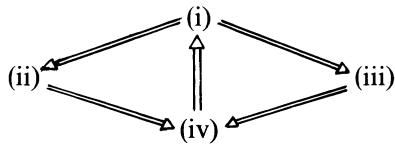
\includegraphics[keepaspectratio]{images/part002_fd83f186.jpg}}

若 \(u\) 是满射，则它是一个严格态射 (IV, 第 28 页, 定理 1)，于是对每个半范数 \(p \in \mathrm{S}(\mathrm{E})\)，存在半范数 \(q \in \mathrm{S}(\mathrm{F})\)，使得对所有 \(y \in \mathrm{F}\)（满足 \(q(y) \leqslant 1\) 者），存在 \(x \in \mathrm{E}\) 满足 \(p(x) \leqslant 1\) 且 \(u(x) = y\)。我们立即推出 (i) 蕴含 (ii) 与 (iii)。显然 (ii) 蕴含 (iv)。

为证 (iii) 蕴含 (iv)，设 \(p\) 与 \(q\) 如 (iii) 所述。设 \(y \in \mathbf{F}\)，由 (iii)，存在 \(x\)（属于 \(\mathbf{E}\)）使得 \(q(u(x) - y) = 0\)。若 \(f \in \mathbf{F}'\) 满足 \(|f \circ u| \leqslant p\)，则有 \(f(u(x) - y) = 0\)，于是

\[
\left| f (y) \right| = \left| f (u (x)) \right| \leqslant p (x)
\]

从而关系式 (1) 成立。

最后证明 (iv) 蕴含 (i)。设 \(p \in \mathrm{S}(\mathrm{E})\)，设 \(q\) 是诸函数 \(|f|\)（\(f \in \mathrm{F}'\) 取遍满足 \(|f \circ u| \leqslant p\) 者）的上包络。由 (iv)，\(q\) 在 \(\mathrm{F}\) 上有限，且显然是 \(\mathrm{F}\) 上的一个下半连续半范数；由于 \(\mathrm{F}\) 是桶型空间 (III, 第 25 页, 推论)，我们有 \(q \in \mathrm{S}(\mathrm{F})\)。设 \(\mathbf{B}_p\)（相应地，\(\mathbf{B}_q\)）表示所有 \(x \in \mathrm{E}\)（相应地，\(y \in \mathrm{F}\)）中满足 \(p(x) \leqslant 1\)（相应地，\(q(y) \leqslant 1\)）者所成的集。我们有 \(q \circ u \leqslant p\)，于是 \(u(\mathbf{B}_p) \subset \mathbf{B}_q\)。\(u(\mathbf{B}_p)\) 在 \(\mathrm{F}'\) 中的极集由这样的线性型 \(f \in \mathrm{F}'\) 组成：它们满足 \(|f \circ u| \leqslant p\)，从而 \(|f| \leqslant q\)；换句话说，我们得到 \(u(\mathbf{B}_p)^{\circ} \subset \mathbf{B}_q^{\circ}\)，最后，\(\overline{u(\mathbf{B}_p)} = \mathbf{B}_q\) 由双极定理 (II, 第 45 页, 推论 3) 得出。若 \(\mathrm{U}\) 是 \(\mathrm{E}\) 中 0 的一个邻域，则存在 \(p \in \mathrm{S}(\mathrm{E})\) 使得 \(\mathbf{B}_p \subset \mathbf{U}\)，于是 \(\overline{u(\mathbf{U})}\) 包含邻域 \(\mathbf{B}_q\)（即 \(\mathrm{F}\) 中 0 的邻域）。这就蕴含 \(u\) 是满射 (I, 第 17 页, 定理 1)。

推论. --- 设 E 与 F 是 Banach 空间。下列条件等价：

\begin{enumerate}
\def\labelenumi{(\roman{enumi})}
\item
  \(u\) 是满射。
\item
  存在实数 \(r > 0\)，使得 \(\| f \| \leqslant r\) . \(\| {}^t u(f) \|\) 对所有 \(f \in \mathbf{F}'\) 成立。
\item
  对所有 \(y \in F\)，我们有 \(\sup_{\substack{f\in \mathbf{F}^{\prime}\\ |f\circ u|\leqslant 1}} |f(y)| < +\infty\)。
\end{enumerate}

条件 (ii) 与 (iii) 实际上就是命题 4 的条件 (ii) 与 (iv) 在 Banach 空间情形下的重新表述。

\section{紧性判别法}

\subsection{一般注记}

设 A 是拓扑空间 E 的一个子集。为使 A 中点的一个序列 \((x_{n})_{n\in\mathbf{N}}\) 以 E 的一个点 x 为极限点，必须且只需下列条件成立 (GT, I, § 7, No.~3)：

\begin{enumerate}
\def\labelenumi{(\Alph{enumi})}
\tightlist
\item
  对每个整数 \(m \geqslant 0\) 以及每个邻域 \(\mathbf{U}\)（\(x\) 的一个邻域），存在一个整数 \(n \geqslant m\) 使得 \(x_{n} \in \mathbf{U}\)。
\end{enumerate}

形如 \((y_{k})_{k\in\mathbb{N}}\)（其中 \(y_{k}=x_{n_{k}}\)，\((n_{k})_{k\in\mathbb{N}}\) 是严格递增的正整数序列）的序列称为序列 \((x_{n})_{n\in\mathbb{N}}\) 的一个子序列。若序列 \((x_{n})_{n\in\mathbb{N}}\) 存在一个收敛到 x 的子序列，则 x 是 \((x_{n})\) 的一个极限点；反之，若 x 具有可数的基本邻域系，且 x 是序列 \((x_{n})\) 的极限点，则存在 \((x_{n})\) 的一个收敛到 x 的子序列。

根据 GT, IX, § 2, No.~9 的推论，我们断定，当 E 可度量化时，下列条件等价：

\begin{enumerate}
\def\labelenumi{\alph{enumi})}
\item
  集 A 在 E 中相对紧；
\item
  A 中点的每个无穷序列在 E 中有一个极限点；
\item
  从 A 中点的每个无穷序列，可以抽取出一个收敛到 E 中某点的序列。
\end{enumerate}

在本节中，我们将把这个判别法推广到某些不可度量化的拓扑向量空间。下面的命题使我们在许多情形下能把紧集的研究归结为弱紧集的研究。

命题 1. --- 设 E 是一个 Hausdorff 局部凸空间，A 是 E 的一个子集。设 \(E_{\sigma}\) 表示赋以弱化拓扑的空间 E。

\begin{enumerate}
\def\labelenumi{\alph{enumi})}
\item
  若 \(\mathbf{A}\) 中点的每个无穷序列在 \(\mathbf{E}\) 中有一个极限点，则 \(\mathbf{A}\) 在 \(\mathbf{E}\) 中预紧。
\item
  为使 A 在 E 中相对紧，必须且只需它在 E 中预紧且在 \(E_{\sigma}\) 中相对紧。
\end{enumerate}

我们用反证法证明 \(a)\)。若 \(A\) 不是预紧的，则由 GT, II, § 3, No.~7 的定理 3，可知存在一个对称凸邻域 \(V\)（\(E\) 中 0 的邻域），使得 \(A\) 不能被 \(V\) 的有限个平移所覆盖。

换句话说，若 \(x_{0}, x_{1}, \ldots, x_{n-1}\) 是 A 的点，则 \(A \not\subset \bigcup_{0 \leqslant i < n} (x_{i} + V)\)，于是存在 A 的一个点 \(x_{n}\) 使得 \(x_{n} - x_{i} \notin V\) 对 \(0 \leqslant i < n\) 成立。然后，对整数 n 用归纳法，可以构造 A 中点的一个无穷序列 \((x_{n})_{n \in \mathbb{N}}\)，使得 \(x_{n} - x_{m} \notin V\)（当 n \textgreater{} m 时）；由于 V 是对称的，我们还有 \(x_{m} - x_{n} \notin V\)（对 \(m \neq n\)），从而诸集 \(x_{n} + \frac{1}{2}V\) 两两不相交。对 E 中的每个点 x，至多存在一个整数 \(n \geqslant 0\) 使得 \(x_{n} \in x + \frac{1}{2}V\)，因而序列 \((x_{n})_{n \in \mathbb{N}}\) 没有任何极限点。这就证明了 a)。

现在假设 A 在 E 中预紧，并且包含在 \(E_{\sigma}\) 的一个紧子集 B 中。那么 B 在 \(E_{\sigma}\) 中完备，从而在 E 中也完备 (IV, 第 5 页, 注记 2)。我们有 \(\overline{A} \subset B\)，故 A 在 E 中相对紧。逆命题是显然的，b) 随之得证。

\subsection{连续函数集合的简单紧性}

在本节中，X 表示一个紧空间，\(\mathcal{C}_{s}(X)\) 表示 X 上以域 K（等于 R 或 C）为值的连续函数空间。空间 \(\mathcal{C}_{s}(X)\) 赋以 X 上的简单收敛拓扑。

命题 2. --- 设 D 是 X 的一个稠密子集，A 是空间 \(\mathcal{C}_{s}(X)\) 的一个子集。下列条件等价：

\begin{enumerate}
\def\labelenumi{(\roman{enumi})}
\item
  A 在 \(\mathcal{C}_s(\mathbf{X})\) 中相对紧。
\item
  从 \(\mathbf{A}\) 的元素的每个无穷序列，可以抽取一个在 \(\mathcal{C}_s(\mathbf{X})\) 中收敛的序列。
\item
  \(\mathbf{A}\) 的元素的每个无穷序列在 \(\mathcal{C}_s(\mathbf{X})\) 中有一个极限点。
\item
  设 \((f_n)_{n\in \mathbb{N}}\) 是属于 A 的函数序列，\((x_m)_{m\in \mathbb{N}}\) 是 D 的点的序列。若累次极限
\end{enumerate}

\[
\gamma = \lim _ {m \rightarrow \infty} \lim _ {n \rightarrow \infty} f _ {n} (x _ {m}), \quad \delta = \lim _ {n \rightarrow \infty} \lim _ {m \rightarrow \infty} f _ {n} (x _ {m})
\]

存在，则它们相等。此外，我们有 \(\sup_{f\in \mathbf{A}}|f(x)| < +\infty\)（对所有 \(x\in \mathbf{X}\)）。

\begin{enumerate}
\def\labelenumi{(\roman{enumi})}
\tightlist
\item
  \(\Rightarrow\) (ii)：设 \(\overline{\mathbf{A}}\) 是 \(\mathbf{A}\) 在 \(\mathcal{C}_s(\mathbf{X})\) 中的闭包。假设 \(\mathbf{A}\) 是紧的，并考虑函数序列 \(f_n \in \mathbf{A}\)（\(n \in \mathbf{N}\)）。设 \(\phi\) 是连续映射 \(x \mapsto (f_n(x))_{n \in \mathbf{N}}\)（从 \(\mathbf{X}\) 到可度量化空间 \(\mathbf{K}^{\mathbf{N}}\) 中的映射）。像 \(\mathbf{X}'\)（即 \(\mathbf{X}\) 在 \(\phi\) 下的像）是一个紧可度量化空间，因为 \(\mathbf{X}\) 是紧的。设 \(\mathbf{E}\) 是 \(\mathcal{C}_s(\mathbf{X})\) 的闭子空间，由满足下列条件的连续函数 \(f\)（定义在 \(\mathbf{X}\) 上）组成：关系 \(\phi(x) = \phi(y)\) 蕴含 \(f(x) = f(y)\)（\(x, y\) 是 \(\mathbf{X}\) 中任意一对点）。根据 GT, I, § 9, No.~4 的推论 2 与 GT, I, § 5, No.~2 的命题 3，映射 \(f' \mapsto f' \circ \phi\) 是一个同胚 \(\phi^*\)（从 \(\mathcal{C}_s(\mathbf{X}')\) 到 E 上）。因此，集 \(\mathbf{A}' = (\phi^*)^{-1}(\overline{\mathbf{A}})\) 在 \(\mathcal{C}_s(\mathbf{X}')\) 中是紧的，并且显然存在元素 \(f_n'\)（属于 \(\mathbf{A}'\)）使得 \(\phi^*(f_n') = f_n' \circ \phi\) 等于 \(f_n\)。
\end{enumerate}

由于 \(X'\) 是一个紧可度量化空间，存在一个可数稠密子集 \(D'\)（在 \(X'\) 中）(GT, IX, §2, No.~8, 命题 12 与 §2, No.~9, 命题 16)。设 \(T_{1}\)（相应地，\(T_{2}\)）是 \(A'\) 上由 \(D'\)（相应地，\(X'\)）上的简单收敛拓扑诱导的拓扑。那么 \(T_{1}\) 可度量化，\(T_{2}\) 紧且比 \(T_{1}\) 细，因而 \(T_{1}\) 与 \(T_{2}\) 一致；换句话说，\(A'\) 是 \(\mathcal{C}_{s}(X')\) 的一个紧可度量化子空间。从而，存在一个序列 \((f_{n_k}^{\prime})\)（从 \((f_n^{\prime})\) 中抽取），它收敛到某个元素 \(f^{\prime}\)（属于 \(\mathcal{C}_s(\mathbf{X}')\)）。因此，序列 \((f_{n_k})\) 收敛到 \(f = f' \circ \phi\)（在 \(\mathcal{C}_s(\mathbf{X})\) 中）。

\begin{enumerate}
\def\labelenumi{(\roman{enumi})}
\setcounter{enumi}{1}
\item
  \(\Rightarrow\) (iii)：这是显然的。
\item
  \(\Rightarrow\) (iv)：假设 A 的元素的每个无穷序列在 \(\mathcal{C}_s(\mathbf{X})\) 中有一个极限点。设 \(x \in \mathbf{X}\)。映射 \(\phi_x: f \mapsto f(x)\)（从 A 到 K 中的映射）是连续的。于是，\(\phi_x(\mathbf{A})\) 中的每个无穷序列有一个极限点；由于域 K（等于 R 或 C）可度量化，集 \(\phi_x(\mathbf{A})\) 在 K 中相对紧，从而有界。换句话说，我们有 \(\sup_{f \in \mathbf{A}} |f(x)| < \infty\)。
\end{enumerate}

设 \(f_n, x_m, \gamma\) 与 \(\delta\) 如 (iv) 所述。设 \(f\) 是序列 \((f_n)\) 在 \(\mathcal{C}_s(\mathbf{X})\) 中的一个极限点，设 \(x\) 是序列 \((x_m)\) 在紧空间 \(\mathbf{X}\) 中的一个极限点。对每个 \(m\)，映射 \(h \mapsto h(x_m)\)（从 \(\mathcal{C}_s(\mathbf{X})\) 到 \(\mathbf{K}\) 中）是连续的。根据假设，我们有 \(f(x_m) = \lim_{n \to \infty} f_n(x_m)\)，从而 \(\gamma = \lim_{m \to \infty} f(x_m)\)；由于 \(f: \mathbf{X} \to \mathbf{K}\) 连续且 \(x\) 是序列 \((x_m)\) 的一个极限点，我们得到 \(\gamma = f(x)\)。用类似的方式，我们证明等式 \(\delta = f(x)\)，从而 \(\gamma = \delta\)。

\begin{enumerate}
\def\labelenumi{(\roman{enumi})}
\setcounter{enumi}{3}
\tightlist
\item
  \(\Rightarrow\) (i)：假设数 \(f(x)\)（当 \(f\) 取遍 \(\mathbf{A}\) 时）所成的集在 \(\mathbf{K}\) 中有界（对所有 \(x\in \mathbf{X}\)）。这等价于假设闭包 \(\overline{\mathbf{A}}\)（即 \(\mathbf{A}\) 在乘积空间 \(\mathbf{K}^{\mathbf{X}}\) 中的闭包）是紧的 (GT, I, § 9, No.~5)。假设 \(\mathbf{A}\) 在 \(\mathcal{C}_s(\mathbf{X})\) 中不是相对紧的。这就意味着存在一个函数 \(u\in \overline{\mathbf{A}}\) 和一个点 \(a\in \mathbf{X}\)，使得 \(u\) 在 \(a\) 处不连续。于是存在实数 \(\varepsilon >0\)，使得在每个邻域 \(\mathrm{U}\)（\(a\) 的邻域）中，存在一点 \(x\) 满足 \(|u(x) - u(a)|\geqslant \varepsilon\)。
\end{enumerate}

我们将用归纳法构造点的序列 \((x_{n})_{n\in \mathbf{N}}\)（点取自 \(\mathbf{D}\)）与元素的序列 \((f_n)_{n\in \mathbf{N}}\)（元素取自 \(\mathbf{A}\)），使它们满足下列关系：

\[
\left| u (x _ {m}) - u (a) \right| \geqslant \varepsilon \quad \text { for } \quad m \geqslant 1;\tag{$(1)_{m}$}
\]

\[
\left| u (x _ {i}) - f _ {m} (x _ {i}) \right| \leqslant \frac {1}{m + 1} \text { for } 0 \leqslant i \leqslant m - 1;\tag{$(2)_{m}$}
\]

\[
\left| f _ {m} (x _ {i}) - f _ {m} (a) \right| \leqslant \frac {1}{i + 1} \quad \text { for } \quad 0 \leqslant m \leqslant i.\tag{$(3)_{m,i}$}
\]

我们取 \(x_0 = a\)，其中 \(f_0\) 是 A 中任意取的（集 A 非空，否则它在 \(\mathcal{C}_s(\mathbf{X})\) 中将相对紧）。设 \(n \geqslant 1\)，且 \(x_0, x_1, \ldots, x_{n-1}, f_0, f_1, \ldots, f_{n-1}\) 满足关系式 \((1)_m, (2)_m\)（对 \(1 \leqslant m < n\)）与 \((3)_{m,i}\)（对 \(0 \leqslant m \leqslant i < n\)）。由于 \(u\) 属于 \(\overline{\mathbf{A}}\)，存在 \(f_n \in \mathbf{A}\) 满足 \((2)_n\)。设 \(V_n\) 是所有 \(x \in X\) 中满足 \(|f_m(x) - f_m(a)| \leqslant \frac{1}{n+1}\)（对 \(0 \leqslant m \leqslant n\)）者所成的集。由于 \(f_n\) 连续，\(V_n\) 是 \(a\) 的一个邻域；选取一点 \(x_n\)（在 \(D \cap V_n\) 中）使得 \(|u(x_n) - u(a)| \geqslant \varepsilon\)，于是 \((1)_n\) 与 \((3)_{m,n}\) 得到满足。因此，构造可以继续进行。

由于 \(u(\mathbf{X})\) 是 \(\mathbf{K}\) 的一个紧子集，存在一个序列 \((y_k)\)（从 \((x_m)\) 中抽取），使得极限 \(\gamma = \lim_{k\to \infty}u(y_k)\) 存在。由 (2) \(_m\)，我们有 \(u(x_i) = \lim_{n\to \infty}f_n(x_i)\)（对所有 \(i\in \mathbf{N}\)），从而

\[
\gamma = \lim _ {k \rightarrow \infty} \lim _ {n \rightarrow \infty} f _ {n} (y _ {k}).\tag{4}
\]

另一方面，我们有 \(f_{n}(a) = \lim_{i\to \infty}f_{n}(x_{i})\)（由 (3) \(_{m,i}\)），从而 \(f_{n}(a) = \lim_{k\to \infty}f_{n}(y_{k})\)。由于 \(x_0 = a\)，由 (2) \(_{m}\) 推出 \(\lim_{n\to \infty}f_n(a) = u(a)\)。于是，

\[
u (a) = \lim _ {n \rightarrow \infty} \lim _ {k \rightarrow \infty} f _ {n} (y _ {k}).\tag{5}
\]

最后，由 \((1)_{m}\) 得到 \(|\gamma - u(a)| \geqslant \varepsilon\)，于是 \(\gamma \neq u(a)\)。这与断言 (iv) 矛盾；这样我们就证明了 (iv) 蕴含 (i)。

\subsection{Eberlein 定理与 Šmulian 定理}

定理 1 (Eberlein). --- 设 E 是一个 Hausdorff 且拟完备的局部凸空间，T 是 E 上与 E 和 E′ 之间的对偶相容的一个拓扑，A 是 E 的一个子集。为使 A 对于 T 相对紧，必须且只需 A 中点的每个无穷序列对于 T 在 E 中有一个极限点。

所述条件显然是必要的。

现在假设 A 中点的每个无穷序列对于 T 有一个极限点，从而对于较粗的拓扑 \(\sigma(\mathrm{E}, \mathrm{E}')\) 也有一个极限点。那么 A 对于 T 预紧 (IV, 第 32 页, 命题 1)；为使 A 对于 T 相对紧，必须且只需它对于 \(\sigma(\mathrm{E}, \mathrm{E}')\) 相对紧（出处同上）。因此只需对 T 是弱化拓扑 \(\sigma(\mathrm{E}, \mathrm{E}')\) 的情形证明本定理。

设 \(\hat{\mathrm{E}}\) 是 E 的完备化，我们照例把它与代数对偶 \(\mathrm{E}^{\prime *}\)（\(\mathrm{E}'\) 的代数对偶）的一个子空间视为同一 (III, 第 21 页, 定理 2)。设 \(\mathrm{E}_{\sigma}\)、\(\hat{\mathrm{E}}_{\sigma}\) 与 \(\mathrm{E}_{\sigma}^{\prime *}\) 分别表示空间 E、\(\hat{\mathrm{E}}\) 与 \(\mathrm{E}^{\prime *}\)，各赋以拓扑 \(\sigma (\mathrm{E},\mathrm{E}')\)、\(\sigma (\hat{\mathrm{E}},\mathrm{E}')\) 与 \(\sigma (\mathrm{E}^{\prime *},\mathrm{E}^{\prime})\)。

设 \((x_{i}^{\prime})_{i\in\mathbb{I}}\) 是向量空间 \(E^{\prime}\) 在域 K 上的一个基。映射 \(f\mapsto(f(x_{i}^{\prime}))_{i\in\mathbb{I}}\) 是一个同胚 \(\phi\)（从 \(E_{\sigma}^{\prime*}\) 到 \(K^{I}\) 上）；对每个 \(i\in I\)，A 在映射 \(x_{i}^{\prime}\)（从 E 到 K 中的映射）下的像是相对紧的：因为 K 可度量化，且 \(x_{i}^{\prime}(A)\) 的元素的每个无穷序列有一个极限点。由此推出 \(\phi(A)\) 在 \(K^{I}\) 中相对紧，从而闭包 \(\overline{A}\)（A 在 \(E_{\sigma}^{\prime*}\) 中的闭包）是紧的。

其次我们证明 \(\overline{A}\) 包含在 \(\hat{E}\) 中。设 H 是 \(E'\) 的一个等度连续子集；设 X 是它对于 \(\sigma(E', E)\) 的闭包；X 是紧的 (III, 第 17 页, 推论 2)。对每个 \(x \in E'^{*}\)，设 \(\phi_{x}\) 是 \(x' \mapsto \langle x, x' \rangle\) 在 X 上的限制；设 \(\tilde{A} \subset \mathcal{C}_{s}(X)\) 是当 x 取遍 A 时函数 \(\phi_{x}\) 所成的集。鉴于关于 A 的假设，\(\tilde{A}\) 的元素的每个无穷序列在 \(\mathcal{C}_{s}(X)\) 中有一个极限点；由命题 2 (IV, 第 33 页)，集 \(\tilde{A}\) 因而在 \(\mathcal{C}_{s}(X)\) 中相对紧。由此推出，对每个 \(a \in \overline{A}\)，X 上的函数 \(\phi_{a}\) 是连续的。包含关系 \(\overline{A} \subset \hat{E}\) 于是由 III, 第 21 页 的定理 2 得出。

现在我们证明 \(\overline{\mathbf{A}}\) 包含在 E 中。由于 A 在 \(\mathrm{E}_{\sigma}\) 中预紧 (IV, 第 32 页, 命题 1)，它在 \(\mathrm{E}_{\sigma}\) 中有界 (III, 第 3 页, 命题 2)，从而在 E 中也有界 (IV, 第 1 页, 命题 1)。设 C 是 A 在 E 中的闭均衡凸包。那么 C 有界（因 A 有界），从而完备（因 E 拟完备）。换句话说，C 是 \(\hat{\mathrm{E}}\) 的一个凸闭子集，因而也是 \(\hat{\mathrm{E}}_{\sigma}\) 的凸闭子集 (IV, 第 1 页, 命题 1)。由于 \(\mathbf{A} \subset \mathbf{C}\) 且 \(\hat{\mathrm{E}}_{\sigma}\) 的拓扑由 \(\mathrm{E}_{\sigma}^{\prime *}\) 的拓扑诱导，我们有 \(\overline{\mathbf{A}} \subset \mathbf{C}\)，从而 \(\overline{\mathbf{A}} \subset \mathbf{E}\)。

由于 \(E_{\sigma}\) 的拓扑由 \(E_{\sigma}^{\prime*}\) 的拓扑诱导，子集 \(\overline{A}\)（\(E_{\sigma}\) 的子集）是紧的，定理 1 随之得证。

定理 2 (Šmulian). --- 设 E 是一个 Fréchet 空间，A 是 E 的一个子集。设 \(E_{\sigma}\) 表示赋以弱化拓扑的空间 E。下列条件等价：

\begin{enumerate}
\def\labelenumi{(\roman{enumi})}
\item
  A 在 \(\mathrm{E}_{\sigma}\) 中相对紧；
\item
  A 中点的每个无穷序列在 \(\mathrm{E}_{\sigma}\) 中有一个极限点；
\item
  从 \(\mathbf{A}\) 中点的每个无穷序列，可以抽取一个在 \(\mathrm{E}_{\sigma}\) 中收敛的序列。
\end{enumerate}

(i) 与 (ii) 的等价性由 Eberlein 定理得出，且 (iii) 显然蕴含 (ii)。

我们来证明 (i) 蕴含 (iii)。假设 A 在 \(E_{\sigma}\) 中的闭包 B 是紧的，且 \((x_{n})_{n\in\mathbf{N}}\) 是 A 的点的一个序列。设 F 是 E 中包含诸 \(x_{n}\) 的最小闭向量子空间，它是一个满足第一可数公理的 Fréchet 空间。由于 F 在 \(E_{\sigma}\) 中闭，且 F 上的拓扑 \(\sigma(\mathrm{F},\mathrm{F}')\) 由 \(\sigma(\mathrm{E},\mathrm{E}')\) 诱导，集 \(B\cap F\) 对于 \(\sigma(\mathrm{F},\mathrm{F}')\) 是紧的。根据 IV, 第 32 页 的注记，从 \((x_{n})_{n\in\mathbf{N}}\) 中抽取一个对于 \(\sigma(\mathrm{E},\mathrm{E}')\)（或者等价地，对于 \(\sigma(\mathrm{F},\mathrm{F}')\)）收敛的序列，其存在性是下述引理的推论：

引理 1. --- 设 F 是一个满足第一可数公理的 Fréchet 空间。F 的每个对于拓扑 T（由 \(\sigma(\mathrm{F},\mathrm{F}')\) 诱导）紧的子集 C 对于该拓扑可度量化。

由于 \(F'\) 上的预紧收敛拓扑比拓扑 \(\sigma(F', F)\) 细，在 \(F_{s}'\) 中存在一个处处稠密的可数子集 (III, 第 18 页, 推论 1)。于是集 C 可以与 \(K^{D}\) 的一个子集视为同一，且 \(K^{D}\) 的拓扑（它可度量化 (GT, IX, § 2, No.~8)）在 C 上诱导的拓扑比由 \(\sigma(F, F')\) 诱导的拓扑粗，而 C 对于后者是紧的。因此这两个拓扑相同 (GT, I, § 9, No.~4, 推论 3)。

Šmulian 定理可以推广到 E 是一列 Fréchet 空间的严格归纳极限的情形 (IV, 第 67 页, 习题 2)。

\subsection{* 有界连续函数空间的情形}

对每个拓扑空间 X，设 \(\mathcal{C}^{b}(X)\) 表示从 X 到 K 中的所有连续且有界的映射所成的 Banach 空间，赋以由下式定义的范数

\[
\| f \| = \sup _ {x \in X} | f (x) |\tag{6}
\]

(GT, X, § 3, No.~2)。当 X 紧时，X 上的每个连续函数都有界 (GT, IV, § 6, No.~1)，我们把 \(\mathcal{C}(X)\) 记作 \(\mathcal{C}^b(X)\)。

在本节及下一节中，我们将用到下面的引理，它是 Lebesgue 定理 (INT, IV, 第 2 版, § 4, No.~3, 定理 2) 的一个特例，这里用到把 \(\mathcal{C}(\mathrm{X})'\) 的元素解释为 X 上的测度。

引理 2. --- 设 X 是一个紧空间。若序列 \((f_n)_{n\in \mathbf{N}}\) 在 \(\mathcal{C}(\mathbf{X})\) 中有界且在 X 上简单收敛到连续函数 \(f\)，则 \(\mu(f) = \lim_{n\to \infty}\mu(f_n)\) 对每个 \(\mu\)（属于 \(\mathcal{C}(\mathbf{X})'\)）成立。

命题 3. --- 设 X 是一个紧空间，A 是 \(\mathcal{C}(\mathrm{X})\) 的一个有界子集。为使 A 对于简单收敛拓扑相对紧，必须且只需它对于 \(\sigma(\mathcal{C}(\mathrm{X}), \mathcal{C}(\mathrm{X})')\) 相对紧。

简单收敛拓扑是 Hausdorff 的且比 \(\sigma(\mathcal{C}(X), \mathcal{C}(X)')\) 粗，故所述条件是充分的 (GT, I, § 9, No.~4, 推论 3)。

现在假设 A 对于简单收敛拓扑相对紧。设 \((f_{n})_{n\in\mathbf{N}}\) 是 A 的元素的一个序列。由命题 2 (IV, 第 33 页)，存在一个序列 \((f_{n_{k}})\)（从 \((f_{n})\) 中抽取），它简单收敛到一个连续函数 f。由引理 2，有界序列 \((f_{n_{k}})\) 对于 \(\sigma(\mathcal{C}(\mathrm{X}),\mathcal{C}(\mathrm{X})')\) 趋于 f。于是 Šmulian 定理 (IV, 第 36 页, 定理 2) 表明 A 对于 \(\sigma(\mathcal{C}(\mathrm{X}),\mathcal{C}(\mathrm{X})')\) 相对紧。

推论. --- 设 S 是一个拓扑空间，A 是 \(\mathcal{C}^{b}(S)\) 的一个有界子集。下列条件等价：

\begin{enumerate}
\def\labelenumi{(\roman{enumi})}
\item
  A 对于 \(\sigma(\mathcal{C}^b(\mathbf{S}),\mathcal{C}^b(\mathbf{S})')\) 相对紧；
\item
  若 \((f_n)_{n\in \mathbb{N}}\) 是 \(\mathbf{A}\) 的元素的序列，\((x_m)_{m\in \mathbb{N}}\) 是 \(\mathbf{S}\) 的点的序列，且累次极限
\end{enumerate}

\[
\gamma = \lim _ {m \rightarrow \infty} \lim _ {n \rightarrow \infty} f _ {n} (x _ {m}), \quad \delta = \lim _ {n \rightarrow \infty} \lim _ {m \rightarrow \infty} f _ {n} (x _ {m})
\]

存在，则 \(\gamma = \delta\)。

设 X 是 S 的 Stone-Čech 紧化 (GT, IX, § 1, No.~6)，\(\alpha\) 是从 S 到 X 中的典范映射。令 \(D = \alpha(S)\)。映射 \(\phi: f \mapsto f \circ \alpha\) 是从赋范空间 \(\mathcal{C}(X)\) 到赋范空间 \(\mathcal{C}^b(S)\) 上的一个同构；令 \(\tilde{A} = \phi^{-1}(A)\)。由于 X 紧且 D 在 X 中稠密，命题 2 (IV, 第 33 页) 表明条件 (ii) 等价于 \(\tilde{A}\) 对于简单收敛拓扑的紧性。(i) 与 (ii) 的等价性于是由命题 3 得出。*

\subsection{* 弱紧集的凸包}

定理 3 (Krein). --- 设 E 是一个 Hausdorff 且拟完备的局部凸空间，T 是 E 上与 E 和 E′ 之间的对偶相容的一个拓扑。设 A 是 E 的一个对于 T 紧的子集。那么 A 的闭均衡凸包 C 对于 T 是紧的。

我们先作若干约化。

\begin{enumerate}
\def\labelenumi{\Alph{enumi})}
\item
  集 C 对于 \(\mathcal{T}\) 预紧 (II, 第 25 页, 命题 3)，且 A 对于 \(\sigma(\mathrm{E}, \mathrm{E}')\) 紧。根据命题 1 (IV, 第 32 页)，只需证明 C 对于 \(\sigma(\mathrm{E}, \mathrm{E}')\) 紧，于是我们已约化到 \(\mathcal{T} = \sigma(\mathrm{E}, \mathrm{E}')\) 的情形。
\item
  由于 C 对于 \(\sigma(\mathrm{E}, \mathrm{E}')\) 预紧且闭，它对于 E 的初始拓扑有界且闭 (III, 第 3 页, 命题 2 与 IV, 第 1 页, 命题 1)；从而由于 E 拟完备，它是完备的。换句话说，C 是 A 在 E 的完备化 \(\hat{\mathbf{E}}\) 中的闭均衡凸包。由于拓扑 \(\sigma (\hat{\mathbf{E}},\mathrm{E}^{\prime})\) 在 E 上诱导 \(\sigma (\mathrm{E},\mathrm{E}^{\prime})\)，我们已约化到 E 完备的情形。
\item
  设 \(\Gamma\) 是 A 的均衡凸包。那么 C 是 \(\Gamma\) 对于 \(\sigma(E, E')\) 的闭包。由 Eberlein 定理 (IV, 第 35 页, 定理 1)，只需证明点的每个序列 \((x_n)_{n \in \mathbf{N}}\)（点取自 \(\Gamma\)）在 E 中对于 \(\sigma(E, E')\) 有一个极限点。但 \(x_n\) 属于 A 的有限子集 \(\mathbf{B}_n\) 的均衡凸包。设 F 是由可数集 \(\mathbf{B} = \bigcup_{n} \mathbf{B}_n\) 生成的 E 的闭向量子空间。那么 F 完备，F 上的拓扑 \(\sigma(F, F')\) 由 \(\sigma(E, E')\) 诱导，且我们有 \(x_n \in F\)（对所有 \(n \in \mathbf{N}\)）。因而只需证明 \((x_n)_{n \in \mathbf{N}}\) 对于 \(\sigma(F, F')\) 有一个极限点，这就给出了到 E 中存在可数稠密集的情形的约化。
\end{enumerate}

设 A 赋以由 \(\sigma(E, E')\) 诱导的拓扑，这使它成为一个紧空间。我们定义一个线性映射 \(u: E' \to \mathcal{C}(A)\) 如下

\[
u (x ^ {\prime}) (a) = \langle a, x ^ {\prime} \rangle \quad (a \in \mathrm{A}, x ^ {\prime} \in \mathrm{E} ^ {\prime}).\tag{7}
\]

设 \((x_{n}^{\prime})_{n\in\mathbb{N}}\) 是 E′ 中的一个等度连续序列，它对于 \(\sigma(\mathrm{E}^{\prime},\mathrm{E})\) 收敛到 0。那么函数序列 \(u(x_{n}^{\prime})\) 在 \(\mathcal{C}(\mathrm{A})\) 中有界且简单收敛到 0。对每个 \(\mu\in\mathcal{C}(\mathrm{A})^{\prime}\)，由引理 2 (IV, 第 37 页)，我们有 \(\lim_{n\to\infty}\mu(u(x_{n}^{\prime}))=0\)。根据 III, 第 21 页 的注记中给出的判别法，E′ 上的线性型 \(\mu\circ u\) 于是对于 \(\sigma(\mathrm{E}^{\prime},\mathrm{E})\) 连续（对每个 \(\mu\in\mathcal{C}(\mathrm{A})^{\prime}\)）。因此存在一个线性映射 \(v:\mathcal{C}(\mathrm{A})^{\prime}\to\mathrm{E}\) 满足关系式

\[
\langle u (x ^ {\prime}), \mu \rangle = \langle v (\mu), x ^ {\prime} \rangle \quad \left(x ^ {\prime} \in \mathrm{E} ^ {\prime}, \mu \in \mathcal {C} (\mathrm{A}) ^ {\prime}\right).\tag{8}
\]

显然，\(v\) 是连续的，若 \(\mathcal{C}(\mathbf{A})'\) 赋以拓扑 \(\sigma(\mathcal{C}(\mathbf{A})', \mathcal{C}(\mathbf{A}))\)，而 \(E\) 赋以拓扑 \(\sigma(E, E')\)。

Banach 空间 \(\mathcal{C}(\mathrm{A})\) 的（闭）单位球 B 对于拓扑 \(\sigma(\mathcal{C}(\mathrm{A})', \mathcal{C}(\mathrm{A}))\) 是紧的 (III, 第 17 页, 推论 3)。于是，\(v(\mathrm{B})\) 是 E 的一个对于 \(\sigma(\mathrm{E}, \mathrm{E}')\) 的凸均衡紧子集。对每个 \(a \in A\)，连续线性型 \(\varepsilon_a : f \mapsto f(a)\)（\(\mathcal{C}(\mathrm{A})\) 上的连续线性型）属于 B，且由公式 (7) 与 (8) 我们有 \(v(\varepsilon_a) = a\)。因此，\(A \subset v(\mathrm{B})\)，从而 \(C \subset v(\mathrm{B})\)。这就证明了 C 对于 \(\sigma(\mathrm{E}, \mathrm{E}')\) 是紧的。

证毕。

\chapterappendix{仿射变换群的不动点}

\subsection{可解群的情形}

设 \(\mathbf{E}\) 是一个实向量空间，\(\mathbf{K}\) 是 \(\mathbf{E}\) 的一个凸子集。一个映射 \(u: \mathbf{K} \to \mathbf{K}\)，若对 \(x, y\)（属于 \(\mathbf{K}\)）以及对每个实数 \(t\)（属于 \([0, 1]\)），我们有

\[
u (t x + (1 - t) y) = t u (x) + (1 - t) u (y)\tag{1}
\]

就称为一个仿射变换。由关系式 (1) 我们推出

\[
u \left(\sum_ {i \in \mathrm{I}} t _ {i} x _ {i}\right) = \sum_ {i \in \mathrm{I}} t _ {i} u \left(x _ {i}\right)\tag{2}
\]

对每个有限集 I、K 中的点 \(x_{i}\) 以及正实数 \(t_i\)（满足 \(\sum_{i\in I}t_i = 1\)）成立。

设 u 与 v 是 K 上的两个仿射变换，则映射 \(u \circ v\) 是 K 上的一个仿射变换。若 \(v: E \to E\) 是一个满足 \(v(\mathbf{K}) \subset \mathbf{K}\) 的线性映射，则在 K 上与 v 相同的映射 \(u: K \to K\) 是一个仿射变换。

定理 1 (Markoff-Kakutani). --- 设 E 是域 R 上的一个 Hausdorff 局部凸向量空间，K 是 E 的一个非空紧凸子集。设 \(\Gamma\) 是 K 上的一组两两可交换的连续仿射变换。那么存在 K 中的一点 a，使得 \(u(a) = a\) 对所有 \(u \in \Gamma\) 成立。

对每个 \(u \in \Gamma\)，设 \(\mathbf{K}_u\) 是所有 \(x \in \mathbf{K}\) 中满足 \(u(x) = x\) 者所成的集。我们将证明 \(\mathbf{K}_u\) 非空。设 \(x\) 是 \(\mathbf{K}\) 的一个点；对每个整数 \(n \geqslant 1\)，设 \(x_n\) 是元素 \(\frac{1}{n} \sum_{i=0}^{n-1} u^i(x)\)（\(\mathbf{E}\) 中的元素）。由于 \(\mathbf{K}\) 凸且在 \(u\) 下稳定，诸点 \(x_n\) 属于 \(\mathbf{K}\)，且由于 \(\mathbf{K}\) 紧，存在一个极限点 \(a\)（序列 \((x_n)_{n \geqslant 1}\) 的极限点）。映射 \(y \mapsto u(y) - y\)（从 \(\mathbf{K}\) 到 \(\mathbf{E}\) 中的映射）是连续的，因而 \(u(a) - a\) 是序列 \((u(x_n) - x_n)_{n \geqslant 1}\) 的一个极限点。但我们有 \(u(x_n) - x_n = \frac{1}{n} (u^n(x) - x)\)。

由于 K 紧，从而有界 (III, 第 3 页, 命题 2)，序列 \((u^n(x) - x)_{n\geqslant 1}\) 有界；于是序列 \(\left(\frac{1}{n} (u^n (x) - x)\right)_{n\geqslant 1}\) 趋于 0 (III, 第 4 页, 命题 3)，且由于 E 是 Hausdorff 的，我们有 \(u(a) - a = 0\)。因此 \(a\in \mathbf{K}_u\)。

诸集 \(\mathbf{K}_u\) 中的每一个都是紧空间 \(\mathbf{K}\) 的闭凸子集，我们将证明交 \(\bigcap_{u\in \Gamma}\mathbf{K}_u\) 非空。为此只需

证明：对 \(n \geqslant 1\) 以及 \(u_{1}, \ldots, u_{n}\)（属于 \(\Gamma\)），集 \(K_{u_{1}} \cap \ldots \cap K_{u_{n}}\) 非空。n = 1 的情形已经考虑过，我们对 n 用归纳法论证。设 \(n \geqslant 2\)，并令 \(L = K_{u_{1}} \cap \ldots \cap K_{u_{n-1}}\)。由归纳假设，L 是 E 的一个非空紧凸子集。由于 \(u_{n}\) 与 \(u_{1}, \ldots, u_{n-1}\) 交换，我们有 \(u_{n}(L) \subset L\)。把证明的第一部分应用于 \(u_{n}\) 在 L 上诱导的仿射变换，我们断定存在 L 中的一点 a 使得 \(u_{n}(a) = a\)；于是 a 属于 \(K_{u_{1}} \cap \ldots \cap K_{u_{n}}\)，从而该集非空。

推论. --- 设 G 是 K 上连续仿射变换的一个可解群。那么存在 K 中的一点，它在 G 下不变。

根据可解群的定义 (A, I, § 6, No.~4)，存在一个有限递降序列 \((\mathbf{G}_i)_{0\leqslant i\leqslant n}\)（由 \(\mathbf{G}\) 的互不相同的子群组成），使得 \(\mathbf{G}_0 = \mathbf{G}\)，\(\mathbf{G}_n = \{e\}\)，且群 \(\mathbf{G}_{i - 1} / \mathbf{G}_i\) 对 \(1\leqslant i\leqslant n\) 是交换的。设 \(\mathbf{K}_i\) 表示 \(\mathbf{G}_i\) 在 \(\mathbf{K}\) 中的不动点集。那么 \(\mathbf{K}_n = \mathbf{K}\)。此外，对 \(1\leqslant i\leqslant n\)，\(\mathbf{G}_i\) 的每个元素在 \(\mathbf{K}_i\) 上诱导恒等变换；这样，我们就得到交换群 \(\mathbf{G}_{i - 1} / \mathbf{G}_i\) 在 \(\mathbf{K}\) 上的一个作用（若 \(\mathbf{K}_i\) 非空）；由定理 1 可知，不动点集 \(\mathbf{K}_{i - 1}\)（\(\mathbf{G}_{i - 1} / \mathbf{G}_i\) 在 \(\mathbf{K}_i\) 中的不动点集）非空。对 \(i\) 用递降归纳法，我们断定 \(\mathbf{K}_0\) 非空，推论得证。

\subsection{不变均值}

设 X 是一个拓扑空间。设 \(\mathcal{B}(\mathrm{X};\mathbf{R})\) 表示由 X 到 R 中的连续有界映射所成的实向量空间。赋以范数 \(\| f\| = \sup_{x\in \mathbf{X}}|f(x)|\)，它是一个 Banach 空间 (GT, X, § 3, No.~1)；它也是一个序向量空间，其中关系 \(f\geqslant g\) 表示 \(\ll f(x)\geqslant g(x) \text{ 对所有 } x\in \mathbf{X}\gg\)。

定义 1. --- 一个正线性型 \(\mu\)（空间 \(\mathcal{B}(\mathbf{X};\mathbf{R})\) 上的，其中 \(\mathbf{X}\) 是一个拓扑空间），若满足 \(\|\mu\| = 1\)，就称为 \(\mathbf{X}\) 上的一个均值。

* 当 X 紧时，X 上的一个均值是 X 上的一个正测度，且满足 \(\mu(X)=1\)。*

引理 1. --- X 上的均值所成的集 K 是 Banach 空间 \(E = \mathcal{B}(X; \mathbf{R})\) 的对偶的单位球的这样一个子集：其元素是线性型 \(\mu\)（满足 \(\mu(1)=1\) 者）。它是 \(E'\) 的一个对于 \(\sigma(E', E)\) 凸且紧的子集。

设 \(\mu\) 是 \(E\) 上的一个线性型，满足 \(\mu(1) = 1\)。对每个函数 \(f \in E\)，我们定义函数 \(f' \in E\) 为 \(f'(x) = \| f \| - f(x) (x \in X)\)。首先假设 \(\mu\) 是一个均值；对每个 \(f \in E\)，我们有 \(f' \geqslant 0\)，从而 \(\mu(f') \geqslant 0\)，即 \(\mu(f) \leqslant \| f \|\)；因此 \(\|\mu\| \leqslant 1\)。

反之，假设 \(\mu\) 属于 \(E'\)，且 \(\| \mu \| \leqslant 1\)；对每个正函数 \(f \in E\)，我们有 \(\mu(f') \leqslant \| f'\|\)，从而

\[
\| f \| - \mu (f) = \mu \left(f ^ {\prime}\right) \leqslant \| f ^ {\prime} \| \leqslant \| f \|,
\]

最后 \(\mu(f) \geqslant 0\)；于是，\(\mu\) 是一个均值。

显然 K 是凸的；它对于 \(\sigma(\mathrm{E}^{\prime},\mathrm{E})\) 的紧性由 III, 第 17 页 的推论 3 得出。

证毕。

设 \(\Gamma\) 是 X 到 X 中的两两交换的连续映射所成的一个集。设 \(\gamma \in \Gamma\)。对每个函数 \(f \in \mathbf{E}\)，我们有 \(f \circ \gamma \in \mathbf{E}\)；于是我们可以在 X 上的均值所成的集 K 上定义一个仿射变换 \(u_{\gamma}\)，如下

\[
u _ {\gamma} \mu (f) = \mu (f \circ \gamma) (\mu \in \mathrm{K}, f \in \mathrm{E}).
\]

若 K 赋以由 \(\sigma(\mathrm{E}^{\prime},\mathrm{E})\) 诱导的拓扑，则映射 \(u_{\gamma}\) 是连续的。若 \(\gamma\) 是一个同胚，\(u_{\gamma}\mu\) 可由 \(\mu\) 通过结构转移得到。最后，我们有 \(u_{\gamma}u_{\gamma^{\prime}} = u_{\gamma^{\prime}}u_{\gamma}\)（对所有 \(\gamma\)、\(\gamma^{\prime}\)（属于 \(\Gamma\)））。由 Markoff-Kakutani 定理 (IV, 第 39 页, 定理 1)，存在 X 上的一个均值 \(\mu\)，使得 \(u_{\gamma}\mu = \mu\) 对所有 \(\gamma \in \Gamma\) 成立；换句话说，\(\mu\) 满足关系式 \(\mu(f) = \mu(f \circ \gamma)\)（对 \(f \in E\) 与 \(\gamma \in \Gamma\)）。

类似地，定理 1 的推论 (IV, 第 40 页) 蕴含下面的结果：

命题 1. --- 设 X 是一个拓扑空间，G 是一个可解群。我们假设 G 左作用在 X 上，使得对所有 \(g \in G\)，映射 \(x \mapsto g \cdot x\)（从 X 到 X 中的映射）是连续的。那么存在 X 上的一个在 G 下不变的均值。

推论. --- 设 G 是一个可解拓扑群。那么存在 G 上的一个均值，它在左平移与右平移下不变。

只需把命题 1 应用于可解群 \(\mathbf{G} \times \mathbf{G}\) 在 \(\mathbf{G}\) 上通过 \((g, g') \cdot x = gxg'^{-1}\) 的作用。

\subsection{Ryll-Nardzewski 定理}

在本节中，E 表示域 R 上的一个赋范空间，T 表示 E 上的一个 Hausdorff 局部凸拓扑，对于它 E 的范数是下半连续的。这些假设特别在下列情形下满足：

\begin{enumerate}
\def\labelenumi{\alph{enumi})}
\item
  \(\mathcal{T}\) 是由赋范空间 E 的范数诱导的拓扑。
\item
  \(\mathcal{T}\) 是赋范空间 E 的弱化拓扑 \(\sigma (\mathrm{E},\mathrm{E}^{\prime})\)。
\item
  E 是一个赋范空间 F 的对偶且 \(\mathcal{T} = \sigma (\mathrm{F}',\mathrm{F})\)
\end{enumerate}

\(d\) ) 存在两个赋范空间 \(\mathrm{F}_1\) 与 \(\mathrm{F}_2\)，使得 \(\mathrm{E} = \mathcal{L}(\mathrm{F}_1;\mathrm{F}_2)\) 且 \(\mathcal{T}\) 是简单收敛拓扑。

除非另有明确说明，拓扑概念均指拓扑 \(\mathcal{T}\) 而言。

设 K 是 E 的一个凸子集。假设 K（对于拓扑 T）是紧的，且 K 对于由 E 的范数定义的距离满足第一可数公理。

引理 2. --- 假设 K 至少含两个点。对每个 \(\varepsilon > 0\)，存在 K 的一个划分，分成两个非空子集 \(\mathbf{K}_1\) 与 \(\mathbf{K}_2\)，它们具有下列性质：

\begin{enumerate}
\def\labelenumi{\alph{enumi})}
\item
  \(\mathrm{K}_1\) 凸且紧；
\item
  我们有 \(\| x_1 - x_2\| < \varepsilon\)（对每个 \(x_{1}\) 与每个 \(x_{2}\)，二者均属于 \(\mathbf{K}_2\)）。
\end{enumerate}

设 L 是 K 的所有极点所成之集的闭包。由 Krein-Milman 定理 (II, 第 55 页, 定理 1)，K 是 L 的闭凸包。由于 K 至少含两个点，L 亦然。对每个 \(x \in L\)，设 \(A_{x}\) 是所有 \(y \in L\) 中满足 \(\|x - y\| \leqslant \varepsilon/4\) 者所成的集。根据 K 上的假设，存在 L 的一个可数子集 D 使得 \(L = \bigcup_{x \in D} A_{x}\)。由于范数下半连续，诸集

\(A_{x}\) 中的每一个都是闭的。把 Baire 定理 (GT, IX, § 5, No.~3, 定理 1) 应用于紧空间 L，我们看出存在 D 中的一点 a 与 E 中的一个开子集 U，使得 \(L \cap U\) 非空且包含在 \(A_{a}\) 中。由于 L 至少含两个点，且 E 是 Hausdorff 的，我们可以选取 U 使得 \(L \not\subset U\)。

设 M 是 \(L \cap \complement U\) 的闭凸包。对满足 0 \textless{} t \textless{} 1 的每个实数 t，设 \(M_{t}\) 是所有形如 \(tx_{1} + (1 - t)x_{2}\)（其中 \(x_{1} \in M\)、\(x_{2} \in K\)）的向量所成的集；这是 K 的一个非空紧凸子集。我们将用反证法证明 \(M_{t} \neq K\)。假设 \(M_{t} = K\)；那么 K 的每个极点 x 属于 \(M_{t}\)，从而可以写成形式 \(x = tx_{1} + (1 - t)x_{2}\)（其中 \(x_{1} \in M\)、\(x_{2} \in K\)）。这蕴含 \(x = x_{1} = x_{2}\)，于是 \(x \in M\)。由 Krein-Milman 定理 (II, 第 55 页, 定理 1)，我们有 K = M，即 K 是 \(L \cap \complement U\) 的闭凸包。由 II, 第 56 页 的推论，这蕴含 \(L \subset L \cap \complement U\)，它与关系式 \(L \cap U \neq \varnothing\) 矛盾。

令 \(d = \sup_{x \in \mathbf{K}, y \in \mathbf{K}} \| x - y \|\)，并选取实数 \(t\) 满足 \(0 < t < 1\) 与 \(t < \varepsilon / 4d\)。令 \(\mathbf{K}_1 = \mathbf{M}_t\)，\(\mathbf{K}_2 = \mathbf{K} - \mathbf{M}_t\)。由前面的论证，诸集 \(\mathbf{K}_1\) 与 \(\mathbf{K}_2\) 非空，且 \(\mathbf{K}_1\) 凸而紧。设 \(\mathbf{M}'\) 是 \(\mathbf{L} \cap \mathbf{U}\) 的闭凸包。由于 \(\mathbf{K}\) 是集 \(\mathbf{L} = (\mathbf{L} \cap \complement \mathbf{U}) \cup (\mathbf{L} \cap \mathbf{U})\) 的闭凸包，它也是 \(\mathbf{M} \cup \mathbf{M}'\) 的闭凸包。设 \(x_1\) 与 \(x_2\) 是 \(\mathbf{K}_2\) 中的两点；对 \(i = 1, 2\)，存在 \(y_i \in \mathbf{M}\)、\(z_i \in \mathbf{M}'\) 与实数 \(\alpha_i\)，使得 \(0 \leqslant \alpha_i \leqslant 1\) 且 \(x_i = \alpha_i y_i + (1 - \alpha_i) z_i\)。若 \(\alpha_i \geqslant t\)，则 \(x_i = ty_i + (1 - t) \left\{\frac{\alpha_i - t}{1 - t} y_i + \frac{1 - \alpha_i}{1 - t} z_i\right\}\)；这与 \(x_i \notin \mathbf{M}_t\) 的假设矛盾。于是 \(\alpha_i < t\)（对 \(i = 1, 2\)），从而

\[
\left\| x _ {i} - z _ {i} \right\| = \left\| \alpha_ {i} \left(y _ {i} - z _ {i}\right) \right\| = \alpha_ {i} \left\| y _ {i} - z _ {i} \right\| \leqslant \alpha_ {i} d <   d t <   \varepsilon / 4.
\]

对每个点 \(z\)（属于 \(\mathbf{M}'\)），我们有 \(\| z - a \| \leqslant \varepsilon / 4\)（因为 \(\mathrm{L} \cap \mathrm{U} \subset \mathrm{A}_a\)），于是特别地 \(\| z_i - a \| \leqslant \varepsilon / 4\)。这样

\[
\left\| x _ {1} - x _ {2} \right\| \leqslant \sum_ {i = 1} ^ {2} \left(\left\| x _ {i} - z _ {i} \right\| + \left\| z _ {i} - a \right\|\right) <   \varepsilon .
\]

证明完毕。

引理 3. --- 设 G 是 K 上（对于 T）连续的仿射变换所成的一个群。假设 K 非空，且对所有 x、K 中的 y 与 G 中所有 g 有 \(\|gx - gy\| = \|x - y\|\)。那么存在 K 中的一点，它在 G 下不变。

设 \(\mathfrak{J}\) 是 \(K\) 的非空子集中对于 \(G\) 闭、凸且稳定的那些子集所成的族。若 \((L_{\alpha})_{\alpha \in I}\) 是 \(\mathfrak{J}\) 的元素的一个按包含关系全序的族，则集 \(L = \bigcap_{\alpha \in I} L_{\alpha}\) 属于 \(\mathfrak{J}\)。于是 (S, III, § 3, No.~4, 定理 2)，存在

一个元素 \(\mathbf{L}\)（属于 \(\mathfrak{J}\)），它对于包含关系是极小的。我们将证明 \(\mathbf{L}\) 缩为一点。

我们用反证法论证，假设 L 至少含两个不同的点 \(x_{1}\) 与 \(x_{2}\)，令 \(x = (x_{1} + x_{2})/2\)，\(\varepsilon = \|x_{1} - x_{2}\|/2\)。凸紧集 L 对于由范数定义的距离满足第一可数公理 (GT, IX, § 2, No.~8)。于是我们可以应用引理 2，找到 L 的一个紧凸子集 \(L_{1}\)，它异于 \(\varnothing\) 且异于 L，并具有下列性质：

\begin{enumerate}
\def\labelenumi{(\Alph{enumi})}
\tightlist
\item
  对每两个点 \(y_{1}\) 与 \(y_{2}\)（属于 \(L - L_{1}\)），我们有 \(\|y_{1} - y_{2}\| < \varepsilon\)。
\end{enumerate}

我们将用反证法证明 \(gx \in L_{1}\) 对所有 \(g \in G\) 成立。设 \(g \in G\) 使得 \(gx \in L - L_{1}\)，那么我们有

\[
\left\| g x _ {i} - g x \right\| = \left\| x _ {i} - x \right\| = \left\| x _ {1} - x _ {2} \right\| / 2 = \varepsilon ,
\]

（对 \(i = 1, 2\)）。由性质 (A)，我们有 \(gx_{i} \in \mathbf{L}_{1}\)。由于 \(\mathbf{L}_{1}\) 凸，我们断定 \(gx = (gx_{1} + gx_{2}) / 2\) 属于 \(\mathbf{L}_{1}\)，这与假设矛盾。

设 \(L'\) 是 x 的轨道 Gx 的闭凸包。集 \(L'\) 属于 J。由前面的论证，我们有 \(L' \subset L_1\)，从而 \(L' \subset L\)，\(L' \neq L\)。这与 L 的极小性矛盾，证明完成。

定理 2 (Ryll-Nardzewski). --- 设 E 是一个赋范空间，K 是 E 的一个非空凸子集，它对于弱化拓扑 \(\sigma(E, E')\) 是紧的。设 G 是 K 的等距仿射变换所成的一个群。那么存在 K 中的一点，它在 G 下不变。

对每个 \(g \in \mathbf{G}\)，设 \(\mathbf{K}_g\) 表示所有点 \(x\)（属于 \(\mathbf{K}\)）中满足 \(gx = x\) 者所成的集；设 \(\mathbf{K}\) 赋以弱化拓扑；每个集 \(\mathbf{K}_g\) 在紧空间 \(\mathbf{K}\) 中凸且闭。我们将证明交 \(\bigcap_{g \in \mathbf{G}} \mathbf{K}_g\) 非空；为此，只需

证明集 \(K_{g_{1}} \cap \ldots \cap K_{g_{n}}\) 对 G 中任意 \(g_{1}, \ldots, g_{n}\) 都非空。固定 \(g_{1}, \ldots, g_{n}\)，设 H 是 G 的由 \(\{g_{1}, \ldots, g_{n}\}\) 生成的子群。在 K 中选取一点 a，设 L 表示 a 的轨道 Ha 的闭凸包。设 D 是形如 \(\lambda_{1}h_{1}a + \cdots + \lambda_{m}h_{m}a\) 的元素所成的可数集，其中 \(\lambda_{1}, \ldots, \lambda_{m}\) 是满足 \(\lambda_{1} + \cdots + \lambda_{m} = 1\) 的正有理数，而 \(h_{1}, \ldots, h_{m}\) 是 H 中的元素。D 对于强拓扑的闭包 \(\overline{D}\) 是凸的，从而它对于 \(\sigma(\mathrm{E}, \mathrm{E}')\) 是闭的 (IV, 第 4 页, 命题 2)；因此 \(\overline{D} = L\)，这就证明了 L 是一个对于距离 \((x, y) \mapsto \|x - y\|\) 满足第一可数公理的度量空间。现在我们可以应用引理 2。存在 L 中的一点 b，它在 H 下不变，从而 \(b \in K_{g_{1}} \cap \ldots \cap K_{g_{n}}\)。

推论. --- 设 E 是一个自反 Banach 空间，G 是赋范空间 E 的自同构所成的一个群，K 是 E 的一个子集。假设 K 非空、凸、闭、有界且在 G 下稳定。那么存在 K 中的一点，它在 G 下不变。

由于 E 自反，K 对于 \(\sigma(\mathrm{E}, \mathrm{E}')\) 是紧的 (IV, 第 15 页, 定理 1)。此外，G 的每个元素属于 \(\mathcal{L}(\mathrm{E})\)。

\subsection{应用.}

* A) 群的酉表示：

设 E 是一个复希尔伯特空间，G 是一个群，\(\pi\) 是 G 在 E 上的一个酉表示，即从 G 到 E 的自同构群中的一个同态。设 \(E^{G}\) 是 E 中在 \(\pi(\mathbf{G})\) 下不变的所有向量所成的希尔伯特子空间。对每个 \(x \in E\)，设 \(K_{x}\) 是 x 的轨道的闭凸包。在 E 中固定一点 x。

我们将证明 \(K_{x}\) 中存在唯一的一个在 \(\pi(\mathbf{G})\) 下不变的点，即 x 在 \(E^{G}\) 上的投影。由 IV, 第 44 页 的推论（应用于 E 的底实向量空间），\(K_{x}\) 中存在一个在 \(\pi(\mathbf{G})\) 下不变的点；设 a 是这样一个点；那么 \(a \in E^{G}\)。设 P 是所有 \(y \in E\) 中满足 y - x 与 \(E^{G}\) 正交者所成的集；我们立即看出 P 闭、凸且在 \(\pi(\mathbf{G})\) 下不变；因此 \(x \in P\)，从而 \(K_{x} \subset P\)，最后 \(a \in P\)。换句话说，a - x 与 \(E^{G}\) 正交；于是 a 是 x 到 \(E^{G}\) 上的投影。

* B) 希尔伯特空间中算子的迹：

假设表示 \(\pi\) 是不可约的，也就是说，不存在 E 的异于 \(\{0\}\) 且异于 E 的希尔伯特子空间在 \(\pi(\mathbf{G})\) 下不变。设 \(\mathbf{F} = \mathcal{L}^{2}(\mathbf{E})\) 是 E 的所有 Hilbert-Schmidt 自同态所成的希尔伯特空间，赋以内积 \(\langle u|v\rangle = \operatorname{Tr}(u^{*}v)\)。我们定义从 G 到 F 中的一个酉表示 \(\lambda\)，其公式为

\[
\lambda (g). u = \pi (g) u \pi (g) ^ {- 1} \quad (u \in \mathrm{F}, g \in \mathrm{G}).\tag{3}
\]

空间 \(F^{G}\)（E 中在 \(\lambda(\mathbf{G})\) 下不变的所有元素所成的空间）由 E 的与 \(\pi(g)\) 交换（对所有 \(g \in G\)）的 Hilbert-Schmidt 自同态 u 组成。由 Schur 引理，这样的 u 是一个位似。于是我们必须考虑两种情形：

\begin{enumerate}
\def\labelenumi{\arabic{enumi})}
\item
  若 E 是无穷维的，则 \(F^{G} = \{0\}\)；
\item
  若 \(\mathrm{E}\) 是有限维的，则 \(\mathrm{F} = \mathcal{L}(\mathrm{E})\) 且 \(\mathrm{F}^{\mathrm{G}} = \mathbf{C}.1_{\mathrm{E}}\)。
\end{enumerate}

把 \(A\) ) 的结果应用于酉表示 \(\lambda\)，我们得到下面的定理：

设 \(u \in \mathcal{L}^2(\mathrm{E})\)，设 \(\mathbf{A}_u\) 是 \(\mathcal{L}^2(\mathrm{E})\) 中的一个闭凸包，即自同态 \(\pi(g) u\pi(g)^{-1}\)（\(\mathrm{E}\) 的自同态，\(g\) 取遍 \(\mathbf{G}\)）所成之集的闭凸包。若 \(\mathrm{E}\) 是无穷维的，我们有 \(0 \in \mathbf{A}_u\)。若 \(\mathrm{E}\) 是有限维的，维数为 \(d\)，则存在唯一的位似

属于 \(\mathbf{A}_u\)，即投影 \(\frac{1}{d}\mathrm{Tr}(u).1_{\mathrm{E}}\)（\(u\) 到子空间 \(\mathbf{C}.1_{\mathrm{E}}\) 上的投影，该子空间含于 \(\mathcal{L}^2 (\mathrm{E}).\)）。

\begin{enumerate}
\def\labelenumi{\Alph{enumi})}
\setcounter{enumi}{2}
\tightlist
\item
  紧群的 Haar 测度：
\end{enumerate}

设 G 是一个紧群，设 \(E = \mathcal{C}(\mathbf{G}, \mathbf{R})\) 是 G 上所有实值连续函数所成的 Banach 空间，赋以范数

\[
\| f \| = \sup _ {x \in \mathbf {G}} | f (x) |.\tag{4}
\]

对所有 \(x \in G\)，我们用下列公式定义 E 的自同构 \(\gamma_{x}\) 与 \(\delta_{x}\)

\[
\gamma_ {x} f (y) = f \left(x ^ {- 1} y\right), \quad \delta_ {x} f (y) = f (y x)\tag{5}
\]

（对 \(y \in \mathbf{G}\)、\(f \in \mathrm{E}\)）。

设 \(f \in E\)，设 \(\Gamma_f\)（相应地，\(\Delta_f\)）表示所有函数 \(\gamma_x f\)（相应地，\(\delta_x f\)）所成之集（\(x\) 取遍 G）在 E 中的闭凸包。我们将证明存在唯一的常值函数 \(\mu(f)\) 属于 \(\Gamma_f\)，唯一的常值函数 \(\mu'(f)\) 属于 \(\Delta_f\)，并且这两个常数相等。

显然，G 上的一个连续函数在 E 的自同构 \(\gamma_{x}(\text{resp. } \delta_{x})\) 下不变，当且仅当它是常值函数。现在，对 G 中的 x，所有函数 \(\gamma_{x}f(\text{resp. } \delta_{x}f)\) 所成之集在 E 中是紧的，因为映射 \(x \mapsto \gamma_{x}f(\text{resp. } x \mapsto \delta_{x}f)\)（从 G 到 E 中的映射）是连续的 (GT, X, §3, No.~4, 定理 3)。由此 (II, 第 25 页, 命题 3) 推出 \(\Gamma_{f}(\text{resp. } \Delta_{f})\) 是 E 中对于由范数定义的拓扑的紧集，从而对于 \(\sigma(\text{E}, \text{E}')\) 也是紧的。由 Ryll-Nardzewski 定理 (IV, 第 43 页, 定理 2)，\(\Gamma_{f}\) 与 \(\Delta_{f}\) 中存在常值函数。剩下的要证明：若 \(c_{1} \in \Gamma_{f}\) 与 \(c_{2} \in \Delta_{f}\) 是常数，则 \(c_{1} = c_{2}\)。

设 \(\varepsilon > 0\)。根据假设，存在点 \(x_{1}, \ldots, x_{n}, y_{1}, \ldots, y_{n}\)（属于 \(\mathbf{G}\)）与正实数 \(\lambda_{1}, \ldots, \lambda_{n}, \mu_{1}, \ldots, \mu_{m}\)，使得

\[
\lambda_ {1} + \dots + \lambda_ {n} = \mu_ {1} + \dots + \mu_ {m} = 1.\tag{6}
\]

\[
\sup _ {x \in \mathbf {G}} \left| \sum_ {i = 1} ^ {n} \lambda_ {i} f (x _ {i} x) - c _ {1} \right| \leqslant \varepsilon ,\tag{7}
\]

\[
\sup _ {x \in \mathbf {G}} \left| \sum_ {j = 1} ^ {m} \mu_ {j} f (x y _ {j}) - c _ {2} \right| \leqslant \varepsilon .\tag{8}
\]

令 \(r = \sum_{i,j} \lambda_i \mu_j f(x_i y_j)\)。那么 \(r - c_1 = \sum_{j=1}^{m} \mu_j a_j\)，其中 \(a_j = \sum_{i=1}^{n} \lambda_i f(x_i y_j) - c_1\)；由 (7)，我们有 \(|a_j| \leqslant \varepsilon\)（对 \(1 \leqslant j \leqslant m\)），从而 \(|r - c_1| \leqslant \varepsilon\)。类似地，我们证明不等式 \(|r - c_2| \leqslant \varepsilon\)，从而 \(|c_1 - c_2| \leqslant 2\varepsilon\)。由于 \(\varepsilon\) 任意，我们得到 \(c_1 = c_2\)，如所断言。

根据 \(\mu(f)\) 的定义，对每个 \(\varepsilon > 0\)，我们可以找到和为 1 的正数 \(\lambda_1, \ldots, \lambda_n\) 与元素 \(x_1, \ldots, x_n\)（属于 \(\mathbf{G}\)），使得 \(\left|\sum_{i=1}^{n} \lambda_i f(x_i x) - \mu(f)\right| \leqslant \varepsilon\) 对所有 \(x \in \mathbf{G}\) 成立。

直接可知，对 \(f, g\)（属于 \(\mathbf{E}\)）以及每个标量 \(\lambda\)，我们有 \(\Gamma_{f + g} \subset \Gamma_f + \Gamma_g\) 与 \(\Gamma_{\gamma f} = \lambda \Gamma_f\)，从而我们有关系式 \(\mu(f + g) = \mu(f) + \mu(g)\) 与 \(\mu(\lambda f) = \lambda \mu(f)\)。因此，映射 \(\mu : f \mapsto \mu(f)\)（从 \(\mathbf{E}\) 到 \(\mathbf{R}\) 中的映射）是紧空间 \(\mathbf{G}\) 上的一个均值 (IV, 第 40 页)；* 换句话说 \(\mu\) 是 \(\mathbf{G}\) 上的一个正测度，且满足 \(\mu(\mathbf{G}) = 1\)。*

直接可知 \(\mu\) 在 G 的左平移下不变，且等式 \(\mu(f) = \mu'(f)\) 蕴含 \(\mu\) 也在右平移下不变。* 换句话说，\(\mu\) 是 G 上的一个左测度且是一个右测度 (INT, VII, § 1, No.~2, def. 2)。*

\paragraph{* D) 不变测度的存在性：}

设 X 是一个 Hausdorff 拓扑空间，\(\mu\) 是 X 上的一个正有界测度，G 是 X 的同胚所成的一个群。假设对所有 \(g \in G\)，测度 \(g \cdot \mu\)（\(\mu\) 在映射 \(g : X \to X\) 下的像）以 \(\mu\) 为基。设 \(u_g\) 是 X 上的一个正的 \(\mu\)-可积函数，使得 \(g \cdot \mu = u_g \cdot \mu\)。再假设存在 X 上的两个正的 \(\mu\)-可积函数 \(\phi\) 与 \(\psi\)，它们不是 \(\mu\)-零的，且使得 \(\phi \leqslant u_g \leqslant \psi\)（\(\mu\)-几乎处处，对所有 \(g \in G\)）。我们将证明存在 X 上的一个正有界测度 \(v \neq 0\)，它以 \(\mu\) 为基且在 G 下不变。

设 P 是 Banach 空间 \(E = L^{1}(X, \mu)\) 中由满足 \(\phi \leqslant f \leqslant \psi\)（\(\mu\)-几乎处处）的函数 f 的类所成的子集。那么 P 对于弱化拓扑 \(\sigma(E, E')\) 是紧的。映射 \(h \mapsto h \cdot \mu\)（从 P 到 X 上有界实测度所成的 Banach 空间 \(F = \mathcal{M}^{b}(X)\) 中的映射）是从 P 到 E 的一个子集 \(P_{1}\) 上的一个双射，该子集对于拓扑 \(\sigma(F, F')\) 凸且紧。根据假设，\(g \cdot \mu \in P_{1}\) 对所有 \(g \in G\) 成立。设 K 是所有测度 \(g \cdot \mu\) 所成之集的闭凸包。对所有 \(g \in G\)，映射 \(v \mapsto g \cdot v\) 是 K 的一个等距仿射变换。由 Ryll-Nardzewski 定理 (IV, 第 43 页, 定理 2)，存在一个测度 \(v \in K\)，它在 G 下不变。我们有 \(\phi \cdot \mu \leqslant v\)，从而 \(v \neq 0\)。

\closechapterappendix
\exercisesheading

\exercisegroup

\begin{enumerate}
\def\labelenumi{\arabic{enumi})}
\tightlist
\item
  设 \(A\) 是一个无穷集。
\end{enumerate}

\begin{enumerate}
\def\labelenumi{\alph{enumi})}
\tightlist
\item
  设 E 是 \(\overline{\mathcal{K}(\mathbf{A})}\) 在 \(\mathbf{R}\) 上的 Banach 空间，由满足下列条件的实数族 \(x = (x_{\alpha})_{\alpha \in \mathbf{A}}\) 组成：\(\alpha \mapsto x_{\alpha}\) 对于 A 的有限子集的余集滤子趋于 0，赋以范数 \(\| x\| = \sup_{\alpha \in \mathbf{A}}|x_{\alpha}|\)（当 \(\mathbf{A} = \mathbf{N}\) 时，这个空间记作 \(c_0\) 或 \(c_0(\mathbf{N})\)。证明 E 上的每个连续线性型都可以唯一地写成 \(x \mapsto \sum_{\alpha \in \mathbf{A}} u_{\alpha} x_{\alpha}\)，其中 \((u_{\alpha})_{\alpha \in \mathbf{A}}\) 是一个满足 \(\sum_{\alpha \in \mathbf{A}} |u_{\alpha}| < +\infty\) 的族；于是 E 的对偶 \(\mathrm{E}'\)
\end{enumerate}

可以（作为非拓扑向量空间）与空间 \(\ell^1 (\mathbf{A})\) 视为同一 (I, 第 4 页, 例)。\(b)\) 设 \(\mathrm{F}\) 是 Banach 空间 \(\ell^1 (\mathbf{A})\) (I, 第 4 页, 例)（当 \(\mathbf{A} = \mathbf{N}\) 时，也记作 \(\ell^1\)）。证明 \(\mathrm{F}\) 上的每个连续线性型都可以唯一地写成 \(x\mapsto \sum_{\alpha \in \mathbf{A}}u_{\alpha}x_{\alpha}\)，其中 \((u_{\alpha})_{\alpha \in \mathbf{A}}\) 是一个有界的实数族；于是 \(\mathrm{F}'\)（\(\mathrm{F}\) 的对偶）可以（作为非拓扑向量空间）与空间 \(\mathcal{B}(\mathbf{A}) = \ell^{\infty}(\mathbf{A})\) 视为同一。

\begin{enumerate}
\def\labelenumi{\alph{enumi})}
\setcounter{enumi}{2}
\tightlist
\item
  设 B 是任意一个集，\((c_{\alpha \beta})_{(\alpha ,\beta)\in \mathrm{A}\times \mathrm{B}}\) 是任意一个 \(\geqslant 0\) 的数族。设 G 是由满足下列条件的实数族 \(x = (x_{\alpha})_{\alpha \in \mathbf{A}}\) 所成的向量空间：对每个 \(\beta \in \mathbf{B}\)，我们有 \(p_{\beta}(x) = \sum_{\alpha \in \mathbf{A}}c_{\alpha \beta}|x_{\alpha}| < + \infty\)；诸 \(p_{\beta}\) 是 G 上的半范数。为使 G（赋以由该半范数族定义的拓扑）是 Hausdorff 的，必须且只需：对每个 \(\alpha \in \mathbf{A}\)，至少存在一个 \(\beta \in \mathbf{B}\) 使得 \(c_{\alpha \beta} > 0\)。证明这时 \(\mathbf{G}\) 完备，且 \(\mathbf{G}\) 上的每个连续线性型都可以唯一地写成 \(x \mapsto \sum_{\alpha \in \mathbf{A}} u_{\alpha} x_{\alpha}\)，其中
\end{enumerate}

\((u_{\alpha})_{\alpha \in \mathbf{A}}\) 是满足下列条件的实数族：存在有限多个指标 \(\beta_{i}\in \mathrm{B}(1\leqslant i\leqslant n)\) 与一个数 \(a > 0\)，使得 \(|u_{\alpha}|\leqslant a.c_{\alpha \beta_i}\) 对所有 \(\alpha \in \mathbf{A}\) 与 \(1\leqslant i\leqslant n\) 成立。证明其逆，并把这些结果推广到标量域为 \(\mathbf{C}\) 的情形。

\begin{enumerate}
\def\labelenumi{\arabic{enumi})}
\setcounter{enumi}{1}
\tightlist
\item
  \begin{enumerate}
  \def\labelenumii{\alph{enumii})}
  \tightlist
  \item
    设 F 与 G 是处于分离对偶中的两个向量空间。证明：若 F 对于 \(\sigma(\mathrm{F}, \mathrm{G})\) 相对有界 (III, 第 43 页, 习题 6)，则 G 对于 \(\sigma(\mathrm{G}, \mathrm{F})\) 相对有界。
  \end{enumerate}
\end{enumerate}

\begin{enumerate}
\def\labelenumi{\alph{enumi})}
\setcounter{enumi}{1}
\item
  设 \(\mathbf{F}\) 是一个向量空间，\(\mathbf{G}_1, \mathbf{G}_2\) 是 \(\mathbf{F}^*\) 的两个向量子空间，使得 \(\mathbf{F}\) 与 \(\mathbf{G}_1\) 以及与 \(\mathbf{G}_2\) 都处于分离对偶中。证明：若 \(\mathbf{F}\) 对于 \(\sigma(\mathbf{F}, \mathbf{G}_1)\) 与 \(\sigma(\mathbf{F}, \mathbf{G}_2)\) 都相对有界，则它对于 \(\sigma(\mathbf{F}, \mathbf{G}_1 + \mathbf{G}_2)\) 也相对有界。
\item
  假设 F 具有可数基。证明：对于 \(\mathbf{F}^*\) 的每个与 F 处于分离对偶且具有可数基的向量子空间 G，F 对于 \(\sigma(\mathrm{F},\mathrm{G})\) 相对有界（用归纳法定义 F 与 G 的两个基 \((a_n)\)、\((b_n)\)，使得 \(\langle a_m, b_n \rangle = \delta_{mn}\)）。
\end{enumerate}

\begin{enumerate}
\def\labelenumi{\arabic{enumi})}
\setcounter{enumi}{2}
\tightlist
\item
  设 F 是一个向量空间。证明：对于拓扑 \(\sigma(F, F^{*})\)，F 的每个有界子集都是有限维的。由此推出，若 F 是无穷维的，则在 F 的完备化 \(\hat{F}\)（对于 \(\sigma(F, F^{*})\)）中，存在不含于 F 的任何有界子集的闭包中的紧子集（参看 II, 第 52 页, 命题 10）。
\end{enumerate}

¶ 4) 设 F 与 G 是处于分离对偶中的两个向量空间，G（相应地，F）当后者赋以拓扑 σ(F, G)（相应地，σ(G, F)）时与 F（相应地，G）的对偶视为同一。设 S（相应地，T）是 F（相应地，G）的一个覆盖，由对于 σ(F, G)（相应地，σ(G, F)）凸、均衡且有界的子集组成。证明下列命题等价：

\(\alpha)\) 每个集 \(\mathbf{M} \in \mathfrak{S}\) 对于 \(\mathfrak{T}\)-拓扑预紧。

β) 每个集 \(\mathbf{N} \in \mathfrak{T}\) 对于 \(\mathfrak{S}\)-拓扑预紧。

\(\gamma)\) 在每个集 \(\mathbf{M} \in \mathfrak{S}\) 上，由 \(\mathfrak{T}\)-拓扑诱导的拓扑与由 \(\sigma(\mathrm{F}, \mathrm{G})\) 诱导的拓扑相同。

\(\delta)\) 在每个集 \(\mathbf{N} \in \mathfrak{T}\) 上，由 \(\mathfrak{S}\)-拓扑诱导的拓扑与由 \(\sigma(\mathbf{G}, \mathbf{F})\) 诱导的拓扑相同。

（利用 III, 第 17 页 的命题 5 证明 \(\alpha\) ) 蕴含 \(\delta\) )，并利用 II, 第 74 页 的习题 1 证明 \(\delta\) ) 蕴含 \(\beta\)。）

\begin{enumerate}
\def\labelenumi{\arabic{enumi})}
\setcounter{enumi}{4}
\item
  设 E 与 F 是两个局部凸 Hausdorff 空间，S 是 E 的子集的一个族。为使空间 \(\mathcal{L}(\mathrm{E};\mathrm{F})\) 上的 S-拓扑与向量空间结构相容，必须（且只需，参看 III, 第 13 页, 推论）S 的每个集都在 E 中有界。
\item
  \begin{enumerate}
  \def\labelenumii{\alph{enumii})}
  \tightlist
  \item
    设 E 是一个局部凸 Hausdorff 空间。对 E 上的每个超滤子 U，设 \(U'\) 是以 U 的集的凸包为基本邻域系的滤子。证明：为使 E 的一点对于弱化拓扑是 U 的极限，必须且只需它对于初始拓扑是 \(U'\) 的接触点（利用 II, 第 84 页 的习题 11）。
  \end{enumerate}
\end{enumerate}

\begin{enumerate}
\def\labelenumi{\alph{enumi})}
\setcounter{enumi}{1}
\tightlist
\item
  设 A 是向量空间 E 的一个凸子集，\(T_{1}, T_{2}\) 是 E 上两个局部凸 Hausdorff 拓扑，\(T_{1}^{\prime}, T_{2}^{\prime}\) 是相应的弱化拓扑。证明：若 \(T_{1}\) 在 A 上诱导的拓扑比 \(T_{2}\) 诱导的拓扑细，则 \(T_{1}^{\prime}\) 在 A 上诱导的拓扑比 \(T_{2}^{\prime}\) 在 A 上诱导的拓扑细。
\end{enumerate}

¶ 7) 设 \(\mathbf{F}\) 是直和空间 \(\mathbf{R}^{(\mathbf{N})}\)，\(\mathbf{G}\) 是空间 \(\ell^1 (\mathbf{N})\) (I, 第 4 页, 例)；\(\mathbf{F}\) 与 \(\mathbf{G}\) 通过双线性型

\[
(x, y) \mapsto \sum_ {n} \xi_ {n} \eta_ {n}
\]

置于对偶中，其中 \(x = (\xi_n)\in \mathbf{F}\)，\(y = (\eta_{n})\in \mathbf{G}\)。

\begin{enumerate}
\def\labelenumi{\alph{enumi})}
\tightlist
\item
  证明：在 F 中，每个凸且对于 \(\sigma(F, G)\) 紧的集 K 都是有限维的。（假设相反；设 \((n_k)\) 是一个严格递增的整数序列 \(>0\)，\((a_k)\) 是 K 的点的序列，使得 \(a_k\) 的指标 \(>n_k\) 的分量均为零，但指标 \(n_k\) 的分量 \(\neq 0\)。证明存在一个序列 \((t_k)\)（其中的数 \(>0\)），使得 \(\sum_{k} t_k < +\infty\)，并且在由实数的所有有界序列组成的 Banach 空间 \(\mathcal{B}(N)\) 中，
\end{enumerate}

点 \(\sum_{k} t_k a_k\) 的指标 \(n_i\) 的分量对所有的 \(i\) 都非零；由此推出部分和序列

\(s_{p} = \sum_{k=1}^{p} t_k a_k\) 在 F 中对于 \(\sigma(F, G)\) 不可能有极限点。

\begin{enumerate}
\def\labelenumi{\alph{enumi})}
\setcounter{enumi}{1}
\item
  证明：在 F 中存在对于 \(\sigma(\mathrm{F},\mathrm{G})\) 的无穷维紧集（注意 G 是 F 对于由赋范空间 \(\mathcal{B}(\mathbf{N})\) 的拓扑所诱导的拓扑的对偶）。证明在 F 中存在对于 \(\sigma(\mathrm{F},\mathrm{G})\) 的预紧集，它们不是相对紧的。
\item
  由 a) 与 b) 推出 \(\tau(\mathbf{G},\mathbf{F})=\sigma(\mathbf{G},\mathbf{F})\)，但 \(\tau(\mathbf{G},\mathbf{F})\) 不同于在 F 的对于 \(\sigma(\mathbf{F},\mathbf{G})\) 紧的子集上的一致收敛拓扑。
\end{enumerate}

\begin{enumerate}
\def\labelenumi{\arabic{enumi})}
\setcounter{enumi}{7}
\tightlist
\item
  设 E 是一个无穷维的局部凸可度量化空间，\(E'\) 是它的对偶。为使拓扑 \(\tau(\mathrm{E}, \mathrm{E}')\) 与弱化拓扑 \(\sigma(\mathrm{E}, \mathrm{E}')\) 相同，必须且只需 E 同构于乘积空间 \(R^{N}\)（相应地，\(C^{N}\)）的一个处处稠密的子空间。（注意在 \(E'\) 中，对于由等度连续集组成的有界结构，存在一个由有限维集组成的可数基（III, 第 1 页）；由此推出向量空间 \(E'\) 具有可数基。）
\end{enumerate}

给出一个局部凸 Hausdorff 空间 \(\mathbf{E}\) 的例子，使得初始拓扑与拓扑 \(\sigma(\mathrm{E},\mathrm{E}')\) 和 \(\tau(\mathrm{E},\mathrm{E}')\) 互不相同。

\begin{enumerate}
\def\labelenumi{\arabic{enumi})}
\setcounter{enumi}{8}
\tightlist
\item
  \begin{enumerate}
  \def\labelenumii{\alph{enumii})}
  \tightlist
  \item
    设 E 是一个局部凸、Hausdorff、有界型且拟完备的空间。为使拓扑 \(\tau(\mathrm{E}^{\prime},\mathrm{E})\) 与 \(\sigma(\mathrm{E}^{\prime},\mathrm{E})\) 在 E 的对偶 \(E^{\prime}\) 上相同，必须且只需 E 的拓扑是最细的局部凸拓扑（证明 E 的每个有界子集都是有限维的）。
  \end{enumerate}
\end{enumerate}

\begin{enumerate}
\def\labelenumi{\alph{enumi})}
\setcounter{enumi}{1}
\tightlist
\item
  设 E 是一个局部凸 Hausdorff 空间，\(E'\) 是它的对偶。为使强拓扑 \(\beta(E', E)\)（在 \(E'\) 上）与弱拓扑 \(\sigma(E', E)\) 相同，必须且只需与 E 相伴的有界型空间（III, 第 40 页, 习题 1）的拓扑是 E 上最细的局部凸拓扑。
\end{enumerate}

\begin{enumerate}
\def\labelenumi{\arabic{enumi})}
\setcounter{enumi}{9}
\tightlist
\item
  设 \(\mathbf{E}\) 是一个局部凸 Hausdorff 空间，\(\mathbf{E}'\) 是它的对偶。证明下列命题等价：
\end{enumerate}

α) E 是桶型空间；

β) E' 的每个弱有界子集都等度连续；

\(\gamma)\) \(\mathbf{E}'\) 的每个弱有界子集都是相对弱紧的，且 \(\mathbf{E}\) 的拓扑是 \(\tau (\mathbf{E},\mathbf{E}')\)。

\begin{enumerate}
\def\labelenumi{\arabic{enumi})}
\setcounter{enumi}{10}
\item
  设 E 是一个局部凸 Hausdorff 空间，\(E'\) 是它的对偶，S 是由 E 的有界子集组成的一个覆盖；我们给 \(E'\) 赋以 S-拓扑。证明：为使双线性型 \((x, x') \mapsto \langle x, x' \rangle\) 在 \(E \times E'\) 上连续，必须且只需 E 的拓扑可由单个范数定义，且 S-拓扑是 \(E'\) 上的强拓扑（参看 III, 第 37 页, 习题 2）。
\item
  设 \(E\) 是一个局部凸 Hausdorff 空间，\(E'\) 是它的对偶。
\end{enumerate}

\begin{enumerate}
\def\labelenumi{\alph{enumi})}
\item
  为使在 \(E'\) 中存在一个弱有界且吸收的集，必须且只需 E 的拓扑比一个赋范空间的拓扑粗（参看 IV, 第 47 页, 习题 2）。
\item
  为使在 \(E'\) 中存在一个等度连续且弱完全的集，必须且只需 E 的拓扑比一个赋范空间的拓扑细。
\item
  为使在 \(E'\) 中存在一个等度连续且吸收的集，必须且只需 E 的拓扑可由单个范数定义。
\end{enumerate}

\begin{enumerate}
\def\labelenumi{\arabic{enumi})}
\setcounter{enumi}{12}
\tightlist
\item
  设 \(\mathbf{F}\) 与 \(\mathbf{G}\) 是 \(\mathbf{R}\) 上处于分离对偶中的两个向量空间。
\end{enumerate}

\begin{enumerate}
\def\labelenumi{\alph{enumi})}
\item
  设 A 是 F 中的一个凸集，不含原点，且对于拓扑 \(\sigma(\mathbf{F}, \mathbf{G})\) 紧；设 C 是以 0 为顶点且由 A 生成的凸锥。证明 G 中的极锥 \(C^{\circ}\) 对于拓扑 \(\tau(\mathbf{G}, \mathbf{F})\) 有一个内点：
\item
  反之，设 C 是一个以 0 为顶点的真凸锥，对于 \(\sigma(F, G)\) 闭，且对于拓扑 \(\tau(F, G)\) 有一个内点。证明在 G 中存在一个超平面 H，它对于 \(\sigma(G, F)\) 闭、不含原点，使得 \(H \cap C^{\circ}\) 对于 \(\sigma(G, F)\) 紧，且 \((H \cap C^{\circ}) \cup \{0\}\) 生成 \(C^{\circ}\)。
\end{enumerate}

\begin{enumerate}
\def\labelenumi{\arabic{enumi})}
\setcounter{enumi}{13}
\tightlist
\item
  设 E 是一个局部凸 Hausdorff 且拟完备的空间，\(E'\) 是它的对偶。证明：在 \(E_{1}'\) 上，紧收敛拓扑是与 E 和 \(E'\) 之间的对偶相容、且与 \(\sigma(E', E)\) 在 \(E'\) 的每个等度连续子集上诱导相同拓扑的诸拓扑中最细的一个（参看 IV, 第 48 页, 习题 4）。
\end{enumerate}

¶ 15) a) 设 E 是一个局部凸 Hausdorff 空间，A 是 E 中的一个凸且均衡的集，u 是 E 上的一个线性型。证明：若 \(\mathrm{A} \cap u^{-1}(0)\) 相对于 A 是闭的，则 u 在 A 上的限制连续。（若不然，证明 0 将属于 A 与一个超平面 \(u^{-1}(\alpha)\)（\(\alpha \neq 0\)）的交的闭包；由此推出，若 \(b \in A\) 满足 \(u(b) = -\alpha\)，则点 \(\frac{1}{2}b\) 将属于 \(\mathrm{A} \cap u^{-1}(0)\) 的闭包。）

\begin{enumerate}
\def\labelenumi{\alph{enumi})}
\setcounter{enumi}{1}
\item
  设 E 是一个实的局部凸 Hausdorff 且完备的空间，\(E'\) 是它的对偶。证明：若超平面 \(H'\)（\(E'\) 的）与每个等度连续且弱闭的子集 \(M' \subset E'\) 的交都是弱闭的，则 \(H'\) 是弱闭的（利用 a) 与 III, 第 21 页, 推论 1）。
\item
  设 E 是一个局部凸 Hausdorff 空间，\(E'\) 是它的对偶，C 是 E 中的一个凸、均衡且闭的集。设 u 是 E 上的一个线性型；证明：若 u 在 C 上的限制对于初始拓扑连续，则它对于 \(\sigma(\mathrm{E}, \mathrm{E}')\) 也连续（利用 a)）。用一个例子证明 u 在由 C 生成的向量子空间 M 上的限制未必连续（取 \(E = R^{(N)}\)，赋以范数 \(\|x\| = \sup_{n} |\xi_{n}|\)，并对 C 取一个生成 E 的适当凸集）。
\end{enumerate}

\begin{enumerate}
\def\labelenumi{\arabic{enumi})}
\setcounter{enumi}{15}
\tightlist
\item
  设 F 与 G 是处于分离对偶中的两个向量空间；把 F 上所有线性型 \(x'\)（在 F 的每个对于 \(\sigma(F, G)\) 有界的子集上都有界者）所成的集，称为 G 在 F 的代数对偶 \(F^{*}\) 中的包封；记这个向量子空间为 \(\tilde{G}\)，它含于 \(F^{*}\)，且当 F 赋以与 F 和 G 之间的对偶相容的诸拓扑之一的相配有界型空间（III, 第 40 页, 习题 1）的拓扑时，它就是 F 的对偶。称 G 在 \(F^{*}\) 中是包封的，如果 \(\tilde{G} = G\)。
\end{enumerate}

\begin{enumerate}
\def\labelenumi{\alph{enumi})}
\tightlist
\item
  设 M 是 F 的一个对于拓扑 \(\sigma(\mathrm{F},\mathrm{G})\) 闭的向量子空间。证明：若 G 在 \(F^{*}\) 中是包封的，且 F/M 赋以拓扑 \(\sigma(\mathrm{F}/\mathrm{M},\mathrm{M}^{\circ})\)，则它的对偶在 \((\mathrm{F}/\mathrm{M})^{*}\) 中是包封的。
\item
  设 E 是一个 Hausdorff 局部凸空间，\(E'\) 是它的对偶。为使 E 是有界型的，必须且只需它的拓扑与 \(\tau(\mathrm{E},\mathrm{E}')\) 相同，且 \(E'\) 在 \(E^{*}\) 中是包封的。
\item
  设 \((\mathrm{E}_{i})_{i\in\mathbb{I}}\) 是一个 Hausdorff 局部凸空间族，F 是 \(E_{i}\) 的直和空间，赋以 I, 第 24 页, 习题 14 中定义的拓扑。证明 F 的对偶典范同构于乘积 \(\prod_{i\in I}E_{i}'\)（诸 \(E_{i}\) 的对偶的乘积）中由
\end{enumerate}

所有族 \((x_{i}^{\prime})\)（除可数多个指标外 \(x_{i}^{\prime}=0\)）组成的子空间。（设 \(V_{i}\) 是 \(E_{i}\) 中 0 的任意邻域。证明：若对一个不可数的指标集有 \(x_{i}^{\prime}\neq0\)，则存在一个数 \(\alpha>0\) 与一个不可数集 H⊂I，使得存在 \(x_{i}\in V_{i}\)，它满足 \(\langle x_{i},x_{i}^{\prime}\rangle\geqslant\alpha\)（对所有 \(i\in H\)）；由此推出 \((x_{i}^{\prime})\) 不可能属于 F'。）

\begin{enumerate}
\def\labelenumi{\alph{enumi})}
\setcounter{enumi}{3}
\tightlist
\item
  证明：若 I 不可数，则 \(\mathbf{F}'\) 在 \(\mathbf{F}^*\) 中不是包封的；若取 \(\mathrm{E}_i = \mathbf{R}\)（对所有 \(i \in \mathrm{I}\)），则赋以强拓扑的 \(\mathbf{F}'\) 不完备，且在 \(\mathbf{F}'\) 中存在不是相对弱紧的强有界子集。
\end{enumerate}

\begin{enumerate}
\def\labelenumi{\arabic{enumi})}
\setcounter{enumi}{16}
\item
  设 E 是一个 Hausdorff 局部凸空间，\(E'\) 是它的对偶；在 \(E'\) 中，设 \(B_{1}\) 是凸等度连续集的族，\(B_{2}\) 是凸的相对弱紧子集的族，\(B_{3}\) 是凸的强有界子集的族，\(B_{4}\) 是凸的弱有界子集的族。于是 \(B_{1} \subset B_{2} \subset B_{3} \subset B_{4}\)。给出一个使这四个集族互不相同的空间 E 的例子（对 E 取三个空间的乘积，对它们分别有 \(B_{1} \neq B_{2}\)（参看 IV, 第 49 页, 习题 8），\(B_{2} \neq B_{3}\)（习题 16, d)），\(B_{3} \neq B_{4}\)（III, 第 23 页, 注 2）。
\item
  设 E、F 是两个向量空间，\(E^{*}\)、\(F^{*}\) 分别是它们的代数对偶。证明：若 u 是一个从 \(F^{*}\) 到 E 中的线性映射，它对于拓扑 \(\sigma(F^{*}, F)\) 与 \(\sigma(E, E^{*})\) 连续，则 \(u(F^{*})\) 是有限维的。（利用 IV, 第 27 页 的命题 2 证明 u 是一个严格态射，并由此推出 \(u(F^{*})\) 是 E 的一个极小型子空间（II, 第 85 页, 习题 13）；考虑这个子空间的有界集以结束证明。）
\item
  设 E 与 F 是两个 Hausdorff 局部凸空间，\(E'\) 与 \(F'\) 是它们的对偶。对从 E 到 F 中的连续线性映射所成的空间 \(\mathcal{L}(\mathrm{E};\mathrm{F})\) 的每个子集 H，用 \({}^{t}H\) 表示映射 \(u\in H\) 的转置所成的集。对 E 的每个子集 M（相应地，子集 \(N'\)，它属于 \(F'\)），用 \(\mathrm{H}(\mathrm{M})\)（相应地，\({}^{t}\mathrm{H}(\mathrm{N}')\)）表示当 u 遍历 H 时诸集 \(u(\mathrm{M})\)（相应地，\({}^{t}u(\mathrm{N}')\)）的并。a) 为使 H 等度连续，必须且只需：对每个等度连续子集 \(N'\)（\(F'\) 的），\({}^{t}\mathrm{H}(\mathrm{N}')\) 是 \(E'\) 的一个等度连续子集。
\end{enumerate}

\begin{enumerate}
\def\labelenumi{\alph{enumi})}
\setcounter{enumi}{1}
\item
  设 \(\mathfrak{S}\) 是 E 的有界子集的一个集。证明：H 在 \(\mathcal{L}(\mathrm{E};\mathrm{F})\) 中对于 \(\mathfrak{S}\) -拓扑有界，当且仅当对每个 \(y' \in \mathrm{F}'\)，\({}^{t}\mathrm{H}(y')\) 在 \(\mathrm{E}'\) 中对于 \(\mathfrak{S}\) -拓扑有界。
\item
  设 S 是 E 的有界子集的一个集，J 是 F 的有界子集的一个集，构成 F 的一个适配有界结构（III, 第 3 页, 定义 4）。假设 E' 赋以 S-拓扑，F' 赋以 J-拓扑。于是 \({}^{t}\mathrm{H}\) 等度连续当且仅当对每个集 B ∈ S，H(B) 属于 J。特别地，\({}^{t}\mathrm{H}\) 对于 F' 与 E' 上的强拓扑等度连续，当且仅当 H 在 L(E; F) 中对于有界收敛拓扑有界。
\end{enumerate}

\(d\) ) 由 \(b\) ) 与 \(c\) ) 推出：若 \({}^t\mathrm{H}\) 在 \(\mathcal{L}(\mathrm{F}';\mathrm{E}')\) 中对于简单收敛拓扑有界（当 \(\mathrm{F}'\) 与 \(\mathrm{E}'\) 赋以强拓扑时），则 \({}^t\mathrm{H}\) 对于这些拓扑等度连续。

\begin{enumerate}
\def\labelenumi{\alph{enumi})}
\setcounter{enumi}{4}
\tightlist
\item
  证明：若 E 是桶型空间，则下列性质等价：
\end{enumerate}

α) H 在 \(\mathcal{L}(E; F)\) 中是简单有界的；

β) H 等度连续；

\(\gamma)\) \({}^{t}\mathrm{H}\) 在 \(\mathcal{L}(\mathrm{F}';\mathrm{E}')\) 中（当 \(\mathrm{E}'\) 赋以弱拓扑 \(\sigma (\mathrm{E}',\mathrm{E})\) 时）是简单有界的。

\(\delta)\) \({}^{t}\mathrm{H}\) 当 \(\mathrm{E}'\) 与 \(\mathrm{F}'\) 赋以强拓扑时等度连续。

\begin{enumerate}
\def\labelenumi{\alph{enumi})}
\setcounter{enumi}{5}
\tightlist
\item
  证明：若 E 是次桶型空间（III, 第 44 页, 习题 7），则性质 \(\beta\) 与 \(\delta\)（\(e\) ) 的）等价，且也与下列性质等价：
\end{enumerate}

ε) H 在 \(\mathcal{L}(\mathrm{E};\mathrm{F})\) 中对于有界收敛拓扑有界；

\(\phi)\) \({}^{t}\mathrm{H}\) 在 \(\mathcal{L}(\mathrm{F}';\mathrm{E}')\) 中（当 \(\mathrm{E}'\) 赋以强拓扑时）是简单有界的。

\begin{enumerate}
\def\labelenumi{\alph{enumi})}
\setcounter{enumi}{6}
\tightlist
\item
  证明：若 E 是拟完备的，则 e) 的性质 \(\alpha\) )、\(\gamma\) ) 与 \(\delta\) ) 等价。
\end{enumerate}

\begin{enumerate}
\def\labelenumi{\arabic{enumi})}
\setcounter{enumi}{19}
\tightlist
\item
  设 \(\mathbf{E}\) 是一个 Hausdorff 局部凸空间，\(\mathbf{E}'\) 是它的对偶。
\end{enumerate}

\begin{enumerate}
\def\labelenumi{\alph{enumi})}
\item
  设 M 是 E 的一个闭向量子空间。拓扑 \(\tau(\mathbf{M}, \mathbf{E}'/\mathbf{M}^{\circ})\) 与 \(\tau(\mathbf{E}, \mathbf{E}')\) 在 M 上诱导的拓扑相同，当且仅当 \(E'/M^{\circ}\) 中每个对于弱拓扑 \(\sigma(\mathrm{E}'/\mathrm{M}^{\circ}, \mathrm{M})\) 紧的凸均衡集，都是某个凸均衡且对于 \(\sigma(\mathrm{E}', \mathrm{E})\) 紧的子集（属于 \(E'\)）的典范像（参看 V, 第 73 页, 习题 15）。
\item
  设 N 是 E 的一个稠密向量子空间。若 E 的拓扑在 N 上诱导的拓扑与 \(\tau(\mathrm{N}, \mathrm{E}')\) 相同，证明 E 的拓扑与 \(\tau(\mathrm{E}, \mathrm{E}')\) 相同。
\end{enumerate}

\begin{enumerate}
\def\labelenumi{\arabic{enumi})}
\setcounter{enumi}{20}
\tightlist
\item
  \begin{enumerate}
  \def\labelenumii{\alph{enumii})}
  \tightlist
  \item
    设 E 是一个向量空间，\(E^{*}\) 是它的代数对偶。证明拓扑 \(\tau(\mathrm{E},\mathrm{E}^{*})\) 是最细的局部凸拓扑，且拓扑 \(\tau(\mathrm{E}^{*},\mathrm{E})\) 与 \(\sigma(\mathrm{E}^{*},\mathrm{E})\) 相同。b) 设 \(E^{**}\) 是 \(E^{*}\) 的代数对偶。证明：若 E 是无穷维的，则 E 在 \(E^{**}\) 中对于与 \(E^{**}\) 和 \(E^{*}\) 之间的对偶相容的所有拓扑都稠密，但 \(\tau(\mathrm{E}^{**},\mathrm{E}^{*})\) 在 E 上诱导的拓扑不同于 \(\tau(\mathrm{E},\mathrm{E}^{*})\)。
  \end{enumerate}
\item
  设 E 是一个 Hausdorff 局部凸空间，\(E'\) 是它的对偶，M 是 E 的一个闭子空间。a) 证明：若 E 中一个紧集的闭凸包是紧的，则 \(E'/M^{\circ}\)（视为 M 的对偶）上的紧收敛拓扑是 \(E'\) 上的紧收敛拓扑关于 \(M^{\circ}\) 的商拓扑。
\end{enumerate}

\begin{enumerate}
\def\labelenumi{\alph{enumi})}
\setcounter{enumi}{1}
\tightlist
\item
  证明：若 \(\mathbf{M}\) 是次桶型的，且 \(\mathrm{E}^{\prime} / \mathrm{M}^{\circ}\) 赋以拓扑 \(\beta (\mathrm{E}^{\prime} / \mathrm{M}^{\circ},\mathbf{M})\) 后是有界型的，则拓扑 \(\beta (\mathrm{E}^{\prime} / \mathrm{M}^{\circ},\mathbf{M})\) 是 \(\beta (\mathrm{E}^{\prime},\mathrm{E})\) 关于 \(\mathbf{M}^{\circ}\) 的商拓扑。
\end{enumerate}

\begin{enumerate}
\def\labelenumi{\arabic{enumi})}
\setcounter{enumi}{22}
\item
  给出一个 Hausdorff 局部凸空间族 \((\mathrm{E}_{i})_{i\in\mathrm{I}}\) 的例子，使得从 \(\bigoplus_{i\in I} E_{i}^{\prime}\) 到 \(P = \prod_{i\in I} E_{i}\) 的对偶上的典范映射不是从诸 \(E_{i}^{\prime}\)（赋以弱拓扑 \(\sigma(\mathrm{E}_{i}^{\prime}, \mathrm{E}_{i})\)）的拓扑直和到对偶 \(P^{\prime}\)（赋以 \(\sigma(\mathrm{P}^{\prime}, \mathrm{P})\)）上的同构。
\item
  设 \((\mathrm{E}_{\alpha})_{\alpha\in\mathrm{A}}\) 是一个局部凸 Hausdorff 空间族，E 是一个向量空间，且对每个 \(\alpha\in A\)，设 \(f_{\alpha}\) 是一个从 \(E_{\alpha}\) 到 E 中的线性映射。在 E 上考虑使诸函数 \(f_{\alpha}\) 连续的最细局部凸拓扑 T（II, 第 27 页）；假设 T 是 Hausdorff 的，并用 \(E_{\alpha}^{\prime}\) 表示 \(E_{\alpha}\) 的对偶，用 \(E^{\prime}\) 表示赋以 T 的 E 的对偶。证明：若对每个 \(\alpha\in A\)，\(E_{\alpha}\) 的拓扑与 \(\tau(\mathrm{E}_{\alpha},\mathrm{E}_{\alpha}^{\prime})\) 相同，则拓扑 T 与 \(\tau(\mathrm{E},\mathrm{E}^{\prime})\) 相同。
\item
  \begin{enumerate}
  \def\labelenumii{\alph{enumii})}
  \tightlist
  \item
    证明：每个实（相应地，复）Banach 空间都等距于形如 \(\mathcal{C}(\mathbf{S};\mathbf{R})\)（相应地，\(\mathcal{C}(\mathbf{S};\mathbf{C})\)）的 Banach 空间的一个闭向量子空间，这种空间由定义在一个紧空间 S 上的所有实（相应地，复）连续函数组成（GT, X, § 4, No. 1）（利用 IV, 第 7 页 的公式 (3)）。
  \end{enumerate}
\end{enumerate}

\begin{enumerate}
\def\labelenumi{\alph{enumi})}
\setcounter{enumi}{1}
\tightlist
\item
  由 a) 推出：每个 Hausdorff 局部凸空间 E 都同构于形如 \(\mathcal{C}_{c}(\mathrm{L};\mathbf{R})\)（相应地，\(\mathcal{C}_{c}(\mathrm{L};\mathbf{C})\)）的局部凸空间的一个子空间（GT, X, § 1, No. 6）。特别地，每个 Fréchet 空间都同构于一个空间 \(\mathcal{C}_{c}(\mathrm{L};\mathbf{R})\)（相应地，\(\mathcal{C}_{c}(\mathrm{L};\mathbf{C})\)）的闭子空间，其中 L 是局部紧且可分的。
\end{enumerate}
% semantic-fragments: legacy-input-seam
\relax{}
\exercisegroup

\begin{enumerate}
\def\labelenumi{\arabic{enumi})}
\tightlist
\item
  \begin{enumerate}
  \def\labelenumii{\alph{enumii})}
  \tightlist
  \item
    设 \(\mathbf{E}\) 是一个 Hausdorff 局部凸空间，\(\mathbf{E}'\) 是它的对偶。证明下列性质等价：
  \end{enumerate}
\end{enumerate}

α) E 是次桶型的 (III, 第 44 页, exerc. 7)。

β) E' 中每个强有界子集都是等度连续的。

\(\gamma)\) \(E'\) 中每个强有界子集都是相对弱紧的，并且 \(E\) 的初始拓扑就是 \(\tau(E, E')\) 。

δ) 双对偶 \(E''\) 的强拓扑在 E 上诱导的拓扑与 E 上的初始拓扑相同。

于是，\(\mathbf{E}''\) 的强拓扑的 0 的一个基本邻域系，由对于拓扑 \(\sigma (\mathrm{E}'', \mathrm{E}')\) 而言的闭包组成，这些闭包来自 \(\mathbf{E}\) 的初始拓扑的 0 的一个基本邻域系。

\begin{enumerate}
\def\labelenumi{\alph{enumi})}
\setcounter{enumi}{1}
\tightlist
\item
  证明：若 E 是次桶型的，且它的对偶 \(E'\) 与它的代数对偶 \(E^{*}\) 相同，则 E 的初始拓扑是最细的局部凸拓扑。
\end{enumerate}

¶ 2) a) 证明次桶型空间的任何乘积都是次桶型的。（化归为 Hausdorff 次桶型空间的情形；然后利用 exerc. 1 以及 IV, 第 14 页的命题 15。）

\begin{enumerate}
\def\labelenumi{\alph{enumi})}
\setcounter{enumi}{1}
\tightlist
\item
  给出一个既非有界型亦非桶型的 Hausdorff 次桶型局部凸空间的例子。（按 III, 第 45 页, exerc. 16 的做法，将其中的桶型空间换成次桶型空间，并利用 a)。）
\end{enumerate}

\begin{enumerate}
\def\labelenumi{\arabic{enumi})}
\setcounter{enumi}{2}
\item
  设 E 是一个复 Hausdorff 局部凸空间，\(E_{0}\) 是 E 的底实局部凸空间，并设 \(E^{\prime}\) 与 \(E_{0}^{\prime}\) 分别是 E 与 \(E_{0}\) 的对偶。证明由 \(f \mapsto Rf\) 给出的、从 \(E^{\prime}\) 到 \(E_{0}^{\prime}\) 上的典范 R-线性映射对于 \(E^{\prime}\) 与 \(E_{0}^{\prime}\) 上的 S-拓扑是一个同胚，其中 S 是 E 的有界子集构成的任意一个集合。由此推出从双对偶 \(E^{\prime\prime}\) 到双对偶 \(E_{0}^{\prime\prime}\) 上的典范 R-线性映射的定义，该映射对于弱拓扑 \(\sigma(E^{\prime\prime}, E^{\prime})\) 与 \(\sigma(E_{0}^{\prime\prime}, E_{0}^{\prime})\) ，同样对于强拓扑 \(\beta(E^{\prime\prime}, E^{\prime})\) 与 \(\beta(E_{0}^{\prime\prime}, E_{0}^{\prime})\) ，都是一个同胚；在这个映射下，E（视为嵌入于 \(E^{\prime\prime}\) 中）变换为 \(E_{0}\)（视为嵌入于 \(E_{0}^{\prime\prime}\) 中）。
\item
  设 E 是一个 Hausdorff 次桶型局部凸空间。
\end{enumerate}

\begin{enumerate}
\def\labelenumi{\alph{enumi})}
\tightlist
\item
  证明：若 E 的强对偶 \(E_{b}^{\prime}\) 是有界型的，则 E 的完备化 \(\hat{E}\)（视为 \(E^{\prime*}\) 的一个向量子空间，III, 第 21 页, 定理 2）包含在 E 的双对偶 \(E^{\prime\prime}\) 中。
\item
  我们称 E 是区分的，如果 \(E^{\prime\prime}\) 中每个对于拓扑 \(\sigma(\mathrm{E}^{\prime\prime}, \mathrm{E})\) 有界的子集，都包含在 E 的某个有界子集（对于该拓扑）的闭包之中。证明：E 是区分的，必须且只需它的强对偶 \(E_{b}^{\prime}\) 是桶型的（参见 IV, 第 15 页, 命题 3）。
\end{enumerate}

\begin{enumerate}
\def\labelenumi{\arabic{enumi})}
\setcounter{enumi}{4}
\tightlist
\item
  设 \(\mathbf{E}\) 是一个 Hausdorff 局部凸空间，\(\mathbf{E}'\) 是它的对偶。
\end{enumerate}

\begin{enumerate}
\def\labelenumi{\alph{enumi})}
\item
  要使 \(\mathbf{E}'\) 上的强拓扑与 \(\tau (\mathrm{E}',\mathrm{E})\) 相同，必须且只需 \(\mathbf{E}\) 是半自反的。
\item
  假设 E 是次桶型的。要使 \(E'\) 上的强拓扑与紧收敛拓扑相同，必须且只需 E 是一个 Montel 空间。
\end{enumerate}

¶ 6) 设 F 与 G 是处于分离对偶中的两个向量空间。

\begin{enumerate}
\def\labelenumi{\alph{enumi})}
\tightlist
\item
  证明下列性质等价：
\end{enumerate}

\(\alpha)\) 空间 \(\mathbf{F}\) ，带上一个与 \(\mathbf{F}\) 和 \(\mathbf{G}\) 之间的对偶相容的拓扑，是半自反的；

\(\beta)\) 空间 \(\mathbf{G}\) ，带上 \(\tau (\mathbf{G},\mathbf{F})\) ，是桶型的。

\begin{enumerate}
\def\labelenumi{\alph{enumi})}
\setcounter{enumi}{1}
\tightlist
\item
  证明下列性质等价：
\end{enumerate}

α) 空间 F，带上 τ(F, G)，是自反的；

\(\beta)\) 空间 \(\mathbf{G}\) ，带上 \(\tau (\mathbf{G},\mathbf{F})\) ，是自反的；

γ) F 与 G 分别对于 τ(F, G) 与 τ(G, F) 是桶型的。

\begin{enumerate}
\def\labelenumi{\alph{enumi})}
\setcounter{enumi}{2}
\item
  证明：每个 Hausdorff 局部凸空间 E，带上拓扑 \(\tau(\mathrm{E}, \mathrm{E}')\) ，同构于一个半自反空间 F 关于一个闭子空间的商。（由 III, 第 44 页, exerc. 14, c)，\(E'\) 带上 \(\tau(\mathrm{E}', \mathrm{E})\) 后同构于某个 Hausdorff 桶型空间 G 的一个闭向量子空间 M；取 \(F = G'\) 带上 \(\tau(\mathrm{G}', \mathrm{G})\) ，并利用 IV, 第 10 页的命题 11。）
\item
  设 A 是一个无限集，满足 \(\operatorname{Card}(\mathrm{A}) > \aleph_{1}\) (S, III, §6, exerc. 10)。在乘积空间 \(P = R^{A}\) 中，设 \(E_{0}\) 表示由所有满足如下条件的 \(x = (x_{\alpha})_{\alpha \in \mathrm{A}}\) 组成的处处稠密子空间：除对一个可数的指标集外，均有 \(x_{\alpha} = 0\) ；空间 \(E_{0}\) 是桶型的，并且 P 中由 \(E_{0}\) 与点 \(1_{A}\) （P 中坐标全等于 1 的点）生成的子空间 E 也是桶型的 (III, 第 45 页, exerc. 16)。设 B 是 \(E_{0}\) 中的一个有界子集，它在 P 中的闭包包含 \(1_{A}\) ，并设 J 是 A 的一个基数为 \(\aleph_{1}\) 的子集；设 \(pr_{J}\) 表示从 P 到 \(R^{J}\) 上的投影；证明：B 中存在一个子集 \(B_{J}\) ，其基数 \(\leqslant \aleph_{1}\) ，使得 \(\operatorname{pr}_{J}(B_{J})\) 在 \(R^{J}\) 中的闭包包含 \(1_{J}\) ；于是，集 \(J' \supset J\) 由所有满足如下条件的指标 \(\alpha \in A\) 组成：\(B_{J}\) 中至少有一点，其下标 \(\alpha\) 的坐标 \(\neq 0\) ；该集的基数等于 \(\aleph_{1}\) 。我们定义 \(J_{0} = J\) ，并用归纳法定义 \(J_{n+1} = J'_{n}\) ，令 \(H = \bigcup_{n} J_{n}\) （其基数为 \(\aleph_{1}\) ），并令 \(B_{H} = \bigcup_{n} B_{J_{n}}\) ；证明：\(B_{H}\) 的闭包（从而 B 的闭包）包含点 \((1_{H}, 0) \in R^{H} \times R^{A-H} = P\) ，而该点不属于 \(E_{0}\) 。由此推断：对 E 中每个有界紧集 C，\(C \cap E_{0}\) 在 E 中仍是闭的，并且 E 不是半自反的。
\item
  由 \(d\) 推出：\(\mathrm{E}'\) （即 \(\mathrm{E}\) 的对偶，它可与对偶 \(\mathrm{P}' = \mathbf{R}^{(\mathbf{A})}\) （\(\mathrm{P}\) 的对偶）等同）对于拓扑 \(\tau (\mathrm{E}',\mathrm{E})\) 不是完备的，尽管它对于该拓扑是半自反的（从而是拟完备的）（考虑 \(\mathrm{E}\) 上在 \(\mathrm{E}_0\) 上等于 0 而在点 \(1_{\mathrm{A}}\) 处等于 1 的线性型，并利用 III, 第 21 页, 定理 2）。
\end{enumerate}

\begin{enumerate}
\def\labelenumi{\arabic{enumi})}
\setcounter{enumi}{6}
\item
  设 \((\mathrm{E}_{i})_{i\in\mathbb{I}}\) 是一族 Hausdorff 局部凸空间，P 是诸 \(E_{i}\) 的乘积空间，S 是它们的拓扑直和。证明：要使 P 或 S 是半自反的（相应地，自反的），必须且只需每个 \(E_{i}\) 都是半自反的（相应地，自反的）。
\item
  设 E 是一个 Hausdorff 局部凸空间，它是一个闭向量子空间递增序列 \((E_{n})\) 的严格归纳极限 (II, 第 32 页, 命题 9)。
\end{enumerate}

\begin{enumerate}
\def\labelenumi{\alph{enumi})}
\item
  证明：若每个 \(\mathbf{E}_n\) 的强对偶都是完备的，则 \(\mathbf{E}\) 的强对偶是完备的 (III, 第 20 页, 定理 1)。
\item
  要使 E 是半自反的（相应地，自反的），必须且只需每个 \(E_{n}\) 都是半自反的（相应地，自反的）。
\end{enumerate}

\begin{enumerate}
\def\labelenumi{\arabic{enumi})}
\setcounter{enumi}{8}
\item
  设 \((\mathrm{E}_{\alpha})_{\alpha\in\mathrm{A}}\) 是包含于同一向量空间中的一族 Hausdorff 局部凸空间，它对于关系 \(\supset\) 是有向的，并且当 \(E_{\beta} \subset E_{\alpha}\) 时，\(E_{\beta}\) 的拓扑比 \(E_{\beta}\) 上由 \(E_{\alpha}\) 的拓扑诱导的拓扑更细。设 E 是诸 \(E_{\alpha}\) 的交，带上一个由诸 \(E_{\alpha}\) 的拓扑在 E 上诱导的拓扑取上确界所得的拓扑。证明：若每个 \(E_{\alpha}\) 都是半自反的，则 E 是半自反的（考虑 E 的一个有界子集上的一个超滤子）。
\item
  证明：Montel 空间的任何乘积以及任何拓扑直和都是一个 Montel 空间 \(^{1}\) 。
\item
  设 E 是一个 Hausdorff 局部凸空间，且 E 的强对偶 \(E_{b}^{\prime}\) 是半自反的。a) 证明：在 \(E^{\prime}\) 的每个强有界子集上，由 \(\sigma(E^{\prime}, E^{\prime\prime})\) 与 \(\sigma(E^{\prime}, E)\) 诱导的拓扑相同。
\end{enumerate}

\begin{enumerate}
\def\labelenumi{\alph{enumi})}
\setcounter{enumi}{1}
\tightlist
\item
  由 a) 推出：E 对于拓扑 \(\tau(E, E')\) 是次桶型的（参见 IV, 第 52 页, exerc. 1），并且若 \(\hat{E}\) 是 E 对于该拓扑的完备化，且视为 \(E'^{*}\) 的一个子集 (III, 第 21 页, 定理 2)，则 \(E'' \subset \hat{E}\) 。特别地，若 E 对于 \(\tau(E, E')\) 是拟完备的，则 E 对于该拓扑是自反的。
\end{enumerate}

\(^{1}\) 另一方面，Montel 空间的闭子空间未必是次桶型的，并且 Montel 空间关于闭子空间的商未必是半自反的 (IV, 第 63 页, exerc. 8)。

\begin{enumerate}
\def\labelenumi{\arabic{enumi})}
\setcounter{enumi}{11}
\tightlist
\item
  设 \(\mathbf{E}\) 是一个 Banach 空间，\(\mathbf{E}'\) 是它的对偶。
\end{enumerate}

\begin{enumerate}
\def\labelenumi{\alph{enumi})}
\item
  证明：由 \(x \mapsto d(x, \mathbf{A})\) 给出的、一点 \(x \in \mathbf{E}\) 到一个闭凸集 \(\mathbf{A}\) 的距离，是 \(\mathbf{E}\) 上对于拓扑 \(\sigma(\mathbf{E}, \mathbf{E}')\) 的下半连续函数。
\item
  证明：若 \(\mathrm{E}\) 是自反的，则对每个闭凸子集 \(\mathrm{A}\) （含于 \(\mathrm{E}\) ），存在一点 \(x_0 \in \mathrm{A}\) 使得 \(\| x_0 \|\) 等于 0 到 \(\mathrm{A}\) 的距离（利用 \(a\) ）。若 \(\mathrm{E}\) 的单位球的每个边界点都是极点，则该点是唯一的 (II, 第 54 页, 定义 1)。
\item
  假设 E 是自反的，并设 B 是 E 中一个闭的、凸的且有界的子集；由 a) 与 b) 推出：存在两点 \(x \in \mathbf{A}\) ，\(y \in \mathbf{B}\) ，使得 \(\| x - y \| = d(\mathbf{A}, \mathbf{B})\) （参见 V, 第 71 页, exerc. 8）。
\end{enumerate}

\begin{enumerate}
\def\labelenumi{\arabic{enumi})}
\setcounter{enumi}{12}
\item
  设 \(\mathbf{E}\) 是一个 Banach 空间，\(\mathbf{M}\) 是 \(\mathbf{E}\) 的一个闭向量子空间。证明：若 \(\mathbf{M}\) 与 \(\mathrm{E / M}\) 都是自反的，则 \(\mathbf{E}\) 是自反的。
\item
  设 \(\mathbf{A}\) 是一个无限集。
\end{enumerate}

\begin{enumerate}
\def\labelenumi{\alph{enumi})}
\tightlist
\item
  证明：Banach 空间 \(E = \overline{\mathcal{K}(A)}\) 的强对偶 (IV, 第 47 页, exerc. 1) 可以与 Banach 空间 \(\ell^{1}(A)\) 等同，并且 Banach 空间 \(\ell'(A)\) 的强对偶可以与 Banach 空间 \(\mathcal{B}(A) = \ell^{\infty}(A)\) 等同；由此推出 E 不是自反的，并且 \(E''/E\) 是无限维的（参见 IV, 第 71 页, exerc. 18）。若 A = N，则 E 与 \(E'\) 都是满足第一可数公理的 Banach 空间，但 \(E''\) 不是 (I, 第 25 页, exerc. 1)。
\item
  设 \(B''\) 是 \(E'' = \ell^{\infty}(A)\) 中的单位球，并设 \(B_{0}''\) 是凸集 \(B'' + (B'' \cap E)\) 。证明：\(B_{0}''\) 是 \(E''\) 中对于强拓扑的一个有界闭凸集，其内部非空，但它没有任何极点。若 p 是 \(B_{0}''\) 的度规，证明：带上范数 p 的 \(E''\) 不等距于任何 Banach 空间的对偶，并且 \(B_{0}''\) 对于拓扑 \(\sigma(E'', E')\) 不是闭的（尽管 \(B''\) 对于 \(\sigma(E'', E')\) 是紧的，且 \(B'' \cap E\) 是强闭的）。
\end{enumerate}

¶ 15) 记号与 exerc. 14 中相同。

\begin{enumerate}
\def\labelenumi{\alph{enumi})}
\tightlist
\item
  设 \((x_n')\) 是 \(E'\) 中对于拓扑 \(\sigma(E', E'')\) 收敛于 0 的一个序列；证明：对每个 \(\varepsilon > 0\) ，存在一个有限子集 \(H\) （\(A\) 的），使得 \(\sum_{\alpha \notin H} |x_n'(\alpha)| \leqslant \varepsilon\) 对每个整数 \(n\) 都成立。
\end{enumerate}

（用反证法：若该性质不成立，证明此时存在一个数 \(\delta > 0\) 、整数的一个递增序列 \((n_k)\) 、A 的有限子集的一个递增序列 \((\mathrm{H}_k)\) ，使得 \(\sum_{\alpha \in \mathrm{H}_{k-1}} |x_n'(\alpha)| \leqslant \frac{\delta}{8}\) 对 \(n \geqslant n_k\) 成立，\(\sum_{\alpha \notin \mathrm{H}_k} |x_n'(\alpha)| \leqslant \frac{\delta}{8}\) 对 \(n \leqslant n_k\) 成立，并且

\(\sum_{\alpha \in \mathrm{H}_k - \mathrm{H}_{k-1}} |x_n'(\alpha)| \geqslant \frac{\delta}{2}\) ；证明这导致矛盾（“滑动峰”方法）。）

由此推出序列 \((x_{n}^{\prime})\) 对于强拓扑收敛于 0，尽管强拓扑严格细于拓扑 \(\sigma (\mathrm{E}',\mathrm{E}'')\) 。

\begin{enumerate}
\def\labelenumi{\alph{enumi})}
\setcounter{enumi}{1}
\tightlist
\item
  证明：若 \((x_{n}^{\prime})\) 是 \(E'\) 中对于拓扑 \(\sigma(E', E'')\) 的一个 Cauchy 序列，则它对于该拓扑收敛于 \(E'\) 中的一点；换言之，\(E'\) 对于 \(\sigma(E', E'')\) 是半完备的 (III, 第 7 页) 。（证明：对每个 \(\varepsilon > 0\) ，存在一个有限子集 \(H\) （\(A\) 中的），使得对每个整数 n 都有 \(\sum_{\alpha \notin H} |x_{n}'(\alpha)| \leqslant \varepsilon\) ；按 a) 的方式用反证法，并利用 a)。）
\end{enumerate}

¶ 16) 采用 exerc. 14 的记号，设 E''' 是 \(E'' = \ell^{\infty}(A)\) 的对偶。

\begin{enumerate}
\def\labelenumi{\alph{enumi})}
\item
  设 \(e_{\alpha}\) （\(\alpha \in A\) ）是 \(E''\) 中满足 \(e_{\alpha}(\beta) = \delta_{\alpha \beta}\) （Kronecker 符号）的元素。设 \((\mathbf{K}_n)\) 是 \(A\) 的有限子集的一个序列，两两不相交，并设 \((x_n''')\) 是 \(E'''\) 中的点的一个序列。证明：存在一个严格递增的无穷整数序列 \((n_k)\) （\(>0\) ），使得若令 \(B = \bigcup_k K_{n_k}\) ，则元素 \(y_n' = (x_n'''(\alpha))_{\alpha \in B}\) 属于 \(\ell^1(B)\) 。（设 \(\delta\) 是任意一个 \(>0\) 的数，并设 \((\mathrm{J}_m)_{m \in \mathbb{N}}\) 是 \(\mathbf{N}\) 分成有限集的一个分割。用反证法证明：若 \(x''' \in E'''\) ，则存在一个整数 \(m\) ，使得 \(|\langle x'', x''' \rangle| \leqslant \delta\) 对所有满足下列条件的 \(x'' \in E''\) 成立：\(\| x'' \| \leqslant 1\) 且 \(x''(\alpha) = 0\) ，只要指标 \(\alpha\) 不属于集 \(\bigcup_{n \in J_m} K_n\) 。以适当的方式相继对 \(x_1'', x_2'', ...\) 应用这一结果。）
\item
  由 \(a\) 以及 exerc. 15, a) 推出：若 \((x_{n}^{\prime \prime \prime})\) 是 \(\mathrm{E}'''\) 中对于拓扑 \(\sigma (\mathrm{E}''',\mathrm{E}'')\) 收敛于 0 的一个序列，且 \(\tilde{x}_n^{\prime \prime \prime}\) 是 \(x_{n}^{\prime \prime \prime}\) 在 \(\mathrm{E}''\) 的强闭子空间 E 上的限制，则 \(\lim_{n\to \infty}\| \tilde{x}_n^{\prime \prime \prime}\| = 0\) （在 \(\mathrm{E}'\) 中）。
\item
  由 b) 推出：\(E''\) 的强闭子空间 E 对于强拓扑没有拓扑补。（限于 A = N 的情形，设 \((e_{n}')\) 是 E 上的连续线性型的一个序列，满足 \(\langle x, e_{n}' \rangle = x(n)\) 对所有 \(x \in E\) ；证明序列 \((e_{n}')\) 对于 \(\sigma(\mathrm{E}', \mathrm{E})\) 趋于 0，但 \(e_{n}'\) 不能扩张为连续线性型 \(x_{n}'''\) （\(E''\) 上的），使得序列 \((x_{n}'''')\) 对于 \(\sigma(\mathrm{E}'''', \mathrm{E}'')\) 趋于 0。）
\end{enumerate}

\begin{enumerate}
\def\labelenumi{\arabic{enumi})}
\setcounter{enumi}{16}
\tightlist
\item
  设 E 是一个非自反 Banach 空间，\(E'\) 是它的强对偶，\(E''\) 是 \(E'\) 的强对偶，\(E'''\) 是 \(E''\) 的强对偶，\(E^{IV}\) 是 \(E'''\) 的强对偶。
\end{enumerate}

\begin{enumerate}
\def\labelenumi{\alph{enumi})}
\item
  证明：在 \(E^{\prime\prime}\) 中，\(E^{\prime}\) 与 E 的正交子空间 \(E^{\circ}\) （当 E 视为 \(E^{\prime\prime}\) 的子空间时）是拓扑补，并且 \(E^{\prime\prime}\) 到 \(E^{\prime}\) 上（对于这个分解）的投影是范数为 1 的连续线性映射。与 exerc. 16, c) 相比较，推出 Banach 空间 \(\mathcal{K}(A)\) （作为拓扑向量空间）不同构于任何 Banach 空间的强对偶。
\item
  证明：\(E^{IV}\) 是 \(E^{\circ}\) 与 \(E''\) 的拓扑直和，也是 \(E^{\prime\circ}\) 与 \(E^{\circ\circ}\) 的拓扑直和；我们有 \(E'' \cap E^{\circ\circ} = E\) 。设 v 是 \(E^{IV}\) 到其自身上的线性映射，它在 \(E^{\circ}\) 上是恒同，而在 \(E''\) 上是 \(E''\) 到 \(E^{\circ\circ}\) 上平行于 \(E^{\circ}\) 的投影；证明 v 是一个等距，但对于拓扑 \(\sigma(\mathrm{E}^{\mathrm{IV}}, \mathrm{E}''')\) 不连续。
\end{enumerate}

\begin{enumerate}
\def\labelenumi{\arabic{enumi})}
\setcounter{enumi}{17}
\item
  证明：一个 Banach 空间 E，若其强对偶 \(E'\) 满足第一可数公理，且 E 对于弱化拓扑 \(\sigma(\mathrm{E}, \mathrm{E}')\) 是半完备的 (III, 第 7 页) ，则 E 是自反的（与 IV, 第 54 页, exerc. 15, b) 相比较）。
\item
  设 \(\mathrm{E}\) 是一个 Banach 空间，\(\mathrm{E}'\) 是它的强对偶，\(\mathrm{G}'\) 是 \(\mathrm{E}'\) 的一个对于强拓扑满足第一可数公理的强闭子空间。证明：存在 \(\mathrm{E}\) 的一个可数子集，使得若 \(\mathrm{F}\) 是该子集在 \(\mathrm{E}\) 中生成的闭向量子空间，则 \(\mathrm{G}'\) 等距于 \(\mathrm{F}'\) （\(\mathrm{F}\) 的强对偶）的一个强闭子空间。（设序列 \((x_n')\) 在 \(\mathrm{G}'\) 中强稠密；对每个 \(n\) ，取 \(x_n \in \mathrm{E}\) 使得 \(\| x_n \| \leqslant 1\) 且 \(\langle x_n, x_n' \rangle = \left(1 - \frac{1}{n}\right) \| x_n' \|\) ；证明：强闭子空间 \(F\) 在 \(E\) 中由诸
\end{enumerate}

\[
x _ {n}
\]

生成的强闭子空间 F 即为所求的空间。）

¶ 20) 设 E 是一个 Banach 空间，E' 是它的对偶，B 是 E 中的单位球。要使 B 的每一点对于 B 上由弱化拓扑 σ(E, E') 诱导的拓扑都具有可数的基本邻域系，必须且只需 E' 对于强拓扑满足第一可数公理。（为证明条件是必要的，注意：若 B 的每一点对于弱化拓扑都有可数的基本邻域系，则 B 在 E'' 中对于拓扑 σ(E'', E') 的闭包 B°° 的每一点也是如此。于是存在 E' 中的一个序列 (a'\_n) ，使得 B°° 中 0 的每个 σ(E'', E') 邻域都包含 B°° 与有限多个极集 \{a'\_n\}° 的交；考虑由诸 a'\_n 生成的 E' 的强闭子空间 W' ，以及 W' 在 E'' 中的正交 \(W'^{\circ}\) 。）

\begin{enumerate}
\def\labelenumi{\arabic{enumi})}
\setcounter{enumi}{20}
\tightlist
\item
  设 E 是一个 Banach 空间，\(E'\) 是它的对偶，B 是 E 中的单位球，\(B_{r}'\) 是 \(E'\) 中以 0 为中心、半径为 r 的闭球。
\end{enumerate}

\begin{enumerate}
\def\labelenumi{\alph{enumi})}
\item
  设 \(M_{1}^{\prime}\) ，\(M_{2}^{\prime}\) 是 \(E^{\prime}\) 的两个向量子空间，它们对于弱拓扑 \(\sigma(\mathrm{E}^{\prime}, \mathrm{E})\) 都是处处稠密的。要使 \(\sigma(\mathrm{E}, \mathrm{M}_{1}^{\prime})\) 与 \(\sigma(\mathrm{E}, \mathrm{M}_{2}^{\prime})\) 在 B 上诱导的拓扑相同，必须且只需 \(M_{1}^{\prime}\) 与 \(M_{2}^{\prime}\) 在 \(E^{\prime}\) 中的强闭包相同。
\item
  设 \(M'\) 是 \(E'\) 的一个对于 \(\sigma(E', E)\) 处处稠密的向量子空间；用 \(\mathbf{M}'^{(1)}\) 表示 \(M' \cap B_{1}'\) 在 \(E'\) 中对于拓扑 \(\sigma(E', E)\) 的闭包所生成的向量子空间。要使 \(\mathbf{M}'^{(1)} = E'\) ，必须且只需 \(M' \cap B_{1}'\) 的弱闭包包含一个球 \(B_{r}'\) ，其中 r \textgreater{} 0（利用 \(E'\) 对于强拓扑是桶型的这一事实）。
\item
  设 \(r\) 是这样的数 \(t\) 的上确界：\(\mathbf{M}' \cap \mathbf{B}_1'\) 的弱闭包包含一个球 \(\mathbf{B}_t'\) ；称数 \(r\) 为 \(\mathbf{M}'\) 的特征数。证明：\(r\) 是诸数 \(\sup_{x' \in \mathbf{M}' \cap \mathbf{B}_1'} |\langle x, x' \rangle| / \| x\|\) 的下确界，其中 \(x\) 取遍所有 \(\neq 0\) 且含于 \(E\) 的点（利用 Hahn-Banach 定理）。
\item
  证明：\(1 / r\) 是 \(\| x\|\) 的上确界，其中 \(x\) 取遍 B 在 E 中对于拓扑 \(\sigma (\mathrm{E},\mathbf{M}^{\prime})\) 的闭包（利用 \(c\) ) 与 Hahn-Banach 定理）。
\item
  设 \(M^{\prime\circ}\) 是 \(M^{\prime}\) 在 \(E^{\prime\prime}\) 中的正交；证明：\(r = \inf(\|x + z^{\prime\prime}\|/\|x\|)\) ，其中 \(z^{\prime\prime}\) 取遍 \(M^{\prime\circ}\) ，x 取遍 E 中非零的点（利用 c) 与 Hahn-Banach 定理）。由此推出：要使 \(\mathbf{M}^{\prime(1)} = \mathbf{E}^{\prime}\) ，必须且只需 \(E + M^{\prime\circ}\) 在 \(E^{\prime\prime}\) 中是强闭的（利用 I, 第 17 页的 Banach 定理）。
\end{enumerate}

\(f\) ) 设 \(\mathbf{A} = \mathbf{N}\times \mathbf{N}\) ，\(\mathrm{E} = \overline{\mathcal{K}(\mathbf{A})}\) （参见 IV, 第 54 页, exerc. 14）。在空间 \(\mathrm{E}'' = \ell^{\infty}(\mathrm{A})\) 中，设 \(\mathrm{P}\) 是由所有这样的点 \(x = (x_{ij})\) 组成的向量子空间：\(x_{ij} = x_{0j} / (j + 1)\) 对所有 \(i\geqslant 0\) 。证明：\(\mathbf{P} = \mathbf{M}'^{\circ}\) ，其中 \(\mathbf{M}'\) 是 \(\mathrm{E}'\) 的一个（对于 \(\sigma (\mathrm{E}',\mathrm{E}))\) 处处稠密的向量子空间，但 \(\mathrm{E} + \mathrm{M}'^{\circ} = \mathrm{E} + \mathrm{P}\) 在 \(\mathrm{E}''\) 中不是强闭的；由此推出 \(\mathbf{M}'\) 的特征数为 0。

\begin{enumerate}
\def\labelenumi{\arabic{enumi})}
\setcounter{enumi}{21}
\tightlist
\item
  设 E 是一个 Banach 空间，\(E'\) 是它的对偶，\(M'\) 是 \(E'\) 中的一个强闭子空间，它对于 \(E'\) 上的弱拓扑是处处稠密的。我们称 M' 是不可约的，如果不存在向量子空间 \(N' \neq M'\) （\(M'\) 的），它在 \(E'\) 中是强闭且弱处处稠密的。a) 证明：\(M'\) 不可约的充要条件是正交 \(M'^{\circ}\) （\(M'\) 在 \(E''\) 中的）是 E 的拓扑补（对于 \(E''\) 的强拓扑）。由此推出此时 \(\mathbf{M}^{(1)} = \mathbf{E}'\) (exerc. 21)，并且 E 同构于空间 \(M'\) （带上由 \(E'\) 的强拓扑诱导的拓扑）的强对偶。
\end{enumerate}

\begin{enumerate}
\def\labelenumi{\alph{enumi})}
\setcounter{enumi}{1}
\item
  证明：\(\mathbf{M}'\) 不可约的充要条件是 \(\mathbf{E}\) 中的单位球对于拓扑 \(\sigma (\mathrm{E},\mathbf{M}')\) 是相对紧的（利用 exerc. 21, a)）。
\item
  要使 E （作为拓扑向量空间）同构于某个 Banach 空间的强对偶，必须且只需 \(E'\) 中存在一个不可约子空间。由此给出下述事实的一个新证明：Banach 空间 \(\overline{\mathcal{K}(\mathbf{N})}\) 不同构于任何 Banach 空间的强对偶（参见 IV, 第 55 页, exerc. 16, c)）。
\end{enumerate}

\begin{enumerate}
\def\labelenumi{\arabic{enumi})}
\setcounter{enumi}{22}
\tightlist
\item
  采用与 exerc. 22 相同的记号，假设 \(\mathbf{M}'\) 是不可约的。
\end{enumerate}

\begin{enumerate}
\def\labelenumi{\alph{enumi})}
\item
  要使从 E 到 \(E^{\prime\prime}/M'^{\circ}\) 中的典范映射（它是典范映射 \(E^{\prime\prime} \rightarrow E^{\prime\prime}/M'^{\circ}\) 的限制）是一个 Banach 空间等距，必须且只需 \(M^{\prime}\) 的特征数 (IV, 第 55 页, exerc. 21) 等于 1。这时，称 \(M^{\prime}\) （带上由 \(E^{\prime}\) 的范数诱导的范数）为 E 的预对偶，并且 E 可以（连同其范数）典范地等同于 Banach 空间 \(M^{\prime}\) 的对偶。
\item
  对 E 的每个对于 \(\sigma (\mathrm{E},\mathbf{M}^{\prime})\) 为闭的向量子空间 F ，证明：\(\mathbf{M}'\) 在 F 的对偶 \(\mathrm{F}'\) （它等同于 \(\mathrm{E}^{\prime} / \mathrm{F}^{\circ}\) ）中的典范像是 F 的一个预对偶。
\end{enumerate}

\begin{enumerate}
\def\labelenumi{\arabic{enumi})}
\setcounter{enumi}{23}
\tightlist
\item
  \begin{enumerate}
  \def\labelenumii{\alph{enumii})}
  \tightlist
  \item
    设 \((a_{k})_{1\leqslant k\leqslant n}\) 是赋范空间 \(E\) 中点的一个有限序列，并设 \((\lambda_k)_{1\leqslant k\leqslant n}\) 是数的一个有限序列，诸数 \(>0\) 且满足 \(\sum_{k = 1}^{n}\lambda_{k} < 1\) ；令 \(\mu_{k} = 1 - \sum_{j = 1}^{k - 1}\lambda_{j}\) （对每个 \(k\) ）；那么
  \end{enumerate}
\end{enumerate}

\[
\left\| \sum_ {k = 1} ^ {n} \lambda_ {k} a _ {k} \right\| \leqslant \frac {\lambda_ {n}}{\mu_ {n - 1}} \left\| \mu_ {n - 1} a _ {n} + \sum_ {k = 1} ^ {n - 1} \lambda_ {k} a _ {k} \right\| + \frac {\mu_ {n}}{\mu_ {n - 1}} \left\| \sum_ {k = 1} ^ {n - 1} \lambda_ {k} a _ {k} \right\|.
\]

\begin{enumerate}
\def\labelenumi{\alph{enumi})}
\setcounter{enumi}{1}
\tightlist
\item
  设 \((a_{n})\) 是 E 的单位球中点的一个无穷序列，并设 \((\lambda_{n})\) 是数的一个无穷序列，诸数 \(>0\) 且满足 \(\sum_{n} \lambda_{n} = 1\) 。对每个 \(n > 0\) ，令 \(\mu_{n} = 1 - \sum_{k=1}^{n-1} \lambda_{k}\) ，并令 \(b_{n} = \sum_{k=1}^{n-1} \lambda_{k} a_{k} + \mu_{n} a_{n}\) ；证明：对所有 \(n \geqslant 1\) ，我们有
\end{enumerate}

\[
\left\| \sum_ {k = 1} ^ {n} \lambda_ {k} a _ {k} \right\| \leqslant \mu_ {n} \sum_ {k = 1} ^ {n} \frac {\lambda_ {k} \| b _ {k} \|}{\mu_ {k - 1} \mu_ {k}}.
\]

（用归纳法应用 a)。）

\begin{enumerate}
\def\labelenumi{\alph{enumi})}
\setcounter{enumi}{2}
\tightlist
\item
  设 \((\mathrm{C}_n)\) 是 E 中凸集的一个递减序列，包含于单位球中，且满足 \(d(0,\mathrm{C}_1)\geqslant \theta >0\) （从而更有 \(d(0,\mathrm{C}_n)\geqslant \theta\) 对所有 \(n\) ）。设 \((\lambda_{n})\) 是数的一个序列，诸数 \(>0\) 且满足 \(\sum_{n}\lambda_{n} = 1\) 。证明：存在一个数 \(\alpha\) 使得 \(\theta \leqslant \alpha \leqslant 1\) ，以及 E 的点的一个序列 \((x_{n})\) ，使得 \(x_{n}\in \mathbf{C}_{n}\) 对所有 \(n\) ，\(\| \sum_{n}\lambda_{n}x_{n}\| = \alpha\) ，且对所有 \(n\)
\end{enumerate}

\[
\left\| \sum_ {k = 1} ^ {n} \lambda_ {k} x _ {k} \right\| \leqslant \alpha (1 - \theta \sum_ {j = n + 1} ^ {\infty} \lambda_ {j}).
\]

（取 \(x_{1}\) 使 \(\| x_{1}\|\) 任意接近 \(d(0, \mathrm{C}_{1})\) ，然后用归纳法取 \(x_{n}\) ，使 \(\left\| \sum_{k=1}^{n-1} \lambda_{k} x_{k} + \left(\sum_{j=n}^{\infty} \lambda_{j}\right) x_{n}\right\|\) 任意接近诸数 \(\left\| \sum_{k=1}^{n-1} \lambda_{k} x_{k} + \left(\sum_{j=n}^{\infty} \lambda_{j}\right) y\right\|\) 的下确界，其中 \(y\) 取遍 \(\mathrm{C}_n\) 。然后利用 \(b)\) 。）

¶ 25) 设 E 是一个满足第一可数公理的 Banach 空间。证明下列性质等价：

α) E 不是自反的。

\(\beta)\) 对每个数 \(\theta\) （满足 \(0 < \theta < 1\) ），存在一个序列 \((x_n')\) （在 \(\mathbf{E}'\) 中），使得 \(\| x_n'\| \leqslant 1\) 对所有 \(n\) ，序列 \((x_n')\) 对于 \(\sigma (\mathrm{E}',\mathrm{E})\) 收敛于 0，并且 0 到由诸 \(x_{n}^{\prime}\) 生成的凸集的距离 \(\geqslant \theta\) 。

\(\gamma)\) 对每个数 \(\theta\) （满足 \(0 < \theta < 1\) ）以及每个序列 \(\lambda_{n}\) （诸数 \(>0\) ，满足 \(\sum_{n} \lambda_{n} = 1\) ），存在一个数 \(\alpha\) 使得 \(\theta \leqslant \alpha \leqslant 1\) ，以及点的一个序列 \((y_{n}')\) ，其点属于

E' ，使得 \(\| y_n'\| \leqslant 1\) 对所有 \(n\) ，\(\left\| \sum_{n}\lambda_ny_n'\right\| = \alpha\) ，且 \(\left\| \sum_{k=1}^{n}\lambda_ky_k'\right\| \leqslant \alpha (1 - \theta \sum_{j=n+1}^{\infty}\lambda_j)\) 对所有 \(n\) 。

\(\delta)\) 存在 \(z' \in \mathrm{E}'\) ，使得没有任何 \(x \in \mathrm{E}\) 满足 \(\left|\langle x, z' \rangle\right| = \| x \| \cdot \| z'\|\) （James-Klee 定理）。

（要看 \(\alpha\) ) 蕴含 \(\beta\) )，注意存在 \(z'' \in \mathrm{E}''\) 使得 \(\| z'' \| < 1\) 且 \(d(z'', \mathrm{E}) > \theta\) 。若 \((x_n)\) 是 \(\mathrm{E}\) 中的一个处处稠密序列，求一个序列 \((x_n')\) （在 \(\mathrm{E}'\) 中），使得 \(\| x_n' \| < 1\) ，且 \(\langle x_k, x_n' \rangle = 0\) （对 \(k \leqslant n\) ）以及 \(\langle x_n', z'' \rangle = \theta\) 。要看 \(\beta\) ) 蕴含 \(\gamma\) )，利用 exerc. 24。要看 \(\gamma\) ) 蕴含 \(\delta\) )，证明对每个 \(x \in \mathrm{E}\) 有 \(|\sum_{n} \lambda_n \langle x, y_n' \rangle| < \alpha\) （利用 \(\gamma\) ）。）

\begin{enumerate}
\def\labelenumi{\arabic{enumi})}
\setcounter{enumi}{25}
\tightlist
\item
  我们称局部凸空间 E 具有性质 (GDF)，如果从 E 到某个 Banach 空间 F 中的每个满足下列性质的线性映射 u 都是连续的：在乘积空间 \(E \times F\) 中，u 的图像 \(\Gamma\) 中收敛点列的每个极限仍属于 \(\Gamma\) 。每个 Fréchet 空间都具有性质 (GDF) (I, 第 19 页, 推论 5)；Fréchet 空间族的每个归纳极限也是如此 (II, 第 34 页, 命题 10)。证明：每个具有性质 (GDF) 的 Hausdorff 局部凸空间都是桶型的。（设 V 是 E 中的一个桶，q 是它的度规，H 是 E 带上这个半范数所对应的 Hausdorff 空间；证明典范映射 \(\pi\) （从 E 到完备化 \(\hat{H}\) 中的）是连续的，这要利用性质 (GDF) 以及每个线性型 \(x' \in V^{0}\) 都可以唯一地扩张成 \(\hat{H}\) 上的连续线性型这一事实（这些线性型所成的集是 \(\hat{H}\) 的对偶中的单位球）。）
\end{enumerate}

\exercisegroup

¶ 1) 设 E 是一个可度量的局部凸空间，\(E_{b}^{\prime}\) 是它的强对偶。若 \(E_{b}^{\prime}\) 是可度量的，证明 E 的拓扑可以由单独一个范数定义（利用 III, 第 37 页, exerc. 2 与第 38 页, exerc. 5，以及 E 是有界型的这一事实）。

\begin{enumerate}
\def\labelenumi{\arabic{enumi})}
\setcounter{enumi}{1}
\tightlist
\item
  次桶型空间是半桶型的。我们称一个局部凸空间为 (DF) 空间，如果它是半桶型的，并且其典范有界结构 (III, 第 3 页, 定义 5) 具有可数基。每个赋范空间以及赋范空间序列的每个严格归纳极限 (II, 第 33 页) 都是 (DF) 空间。Fréchet 空间的每个强对偶都是 (DF) 空间。
\end{enumerate}

\begin{enumerate}
\def\labelenumi{\alph{enumi})}
\item
  (DF) 空间的强对偶是 Fréchet 空间。
\item
  设 \(\mathrm{E}\) 是一个 (DF) 空间，\((\mathbf{A}_n)\) 是 \(\mathrm{E}\) 中有界、凸、均衡且闭的子集的一个递增序列，使得 \(\mathrm{E}\) 的每个有界子集都被诸 \(\mathbf{A}_n\) 之一吸收。
\end{enumerate}

  设 U 是诸 \(A_{n}\) 的并；证明：U 在 E 中的闭包 \(\overline{U}\) 恰好是所有这样的 \(x \in E\) 组成的集：\(\lambda x \in U\) 对 \(0 \leqslant \lambda < 1\) 。（若 \(x \notin \lambda U\) 对某个 \(\lambda > 1\) ，则对每个 n，存在线性型 \(x_{n}' \in E'\) 使得 \(x_{n}' \in A_{n}^{\circ}\) 且 \(\langle x, x_{n}' \rangle = \lambda\) ，而序列 \((x_{n}')\) 是等度连续的，从而有一个弱极限点。）

\begin{enumerate}
\def\labelenumi{\alph{enumi})}
\setcounter{enumi}{2}
\tightlist
\item
  证明：若一个 (DF) 空间是桶型的，则它也是有界型的（参见 III, 第 44 页, exerc. 13, b)）。给出非超有界型但是有界型且桶型的 (DF) 空间的例子 (III, 第 46 页, exerc. 22)，以及非桶型但是有界型的 (DF) 空间的例子。
\end{enumerate}

\begin{enumerate}
\def\labelenumi{\arabic{enumi})}
\setcounter{enumi}{2}
\tightlist
\item
  设 \(E\) 是一个可度量的局部凸空间，\(E_b'\) 是它的强对偶。
\end{enumerate}

\begin{enumerate}
\def\labelenumi{\alph{enumi})}
\item
  证明：每个凸均衡子集 \(V'\) （属于 \(E_{b}'\) ）只要吸收 \(E_{b}'\) 的强有界子集，就包含一个（对于强拓扑的）桶，该桶吸收 \(E_{b}'\) 的强有界子集。（设 \((\mathbf{K}_{n}')\) 是 \(E_{b}'\) 的典范有界结构的一个可数基，并设 \(\lambda_{n}\) 使得 \(\lambda_{n}K_{n}' \subset \frac{1}{2}V'\) ；把 exerc. 2, b) 应用于序列 \(A_{n}'\) ，其中 \(A_{n}'\) 是诸 \(\lambda_{j}K_{j}'\) （\(j \leqslant n\) ）的并的凸包。）
\item
  由 \(a\) ) 推出下列性质等价：
\end{enumerate}

α) E 是区分的 (IV, 第 52 页, exerc. 4)。

β) \(E_{b}^{\prime}\) 是次桶型的 (III, 第 44 页, exerc. 7)。

\(\gamma)\) \(\mathrm{E}_b^{\prime}\) 是有界型的。

δ) \(E_{b}^{\prime}\) 是桶型的。

ε) \(E_{b}^{\prime}\) 是超有界型的 (III, 第 45 页, exerc. 19)。

\begin{enumerate}
\def\labelenumi{\alph{enumi})}
\setcounter{enumi}{2}
\tightlist
\item
  证明：若 \(E_{b}^{\prime}\) 是自反的，则 \(\hat{E} = E''\) （它显然是自反的）（参见 IV, 第 52 页, exerc. 4 及第 53 页, exerc. 11）。
\end{enumerate}

\begin{enumerate}
\def\labelenumi{\arabic{enumi})}
\setcounter{enumi}{3}
\tightlist
\item
  设 E 是一个 Hausdorff 局部凸空间，\(E'\) 是它的对偶。若 M 是 E 的一个可度量且区分的 (IV, 第 52 页, exerc. 4) 闭向量子空间，则强拓扑 \(\beta(\mathrm{E}'/\mathrm{M}^{\circ}, \mathrm{M})\) 是按 \(M^{\circ}\) 从强拓扑 \(\beta(\mathrm{E}', \mathrm{E})\) 得到的商拓扑（利用 exerc. 3, b) 与 IV, 第 51 页, exerc. 22, b)）。
\end{enumerate}

¶ 5) 对每个整数 n \textgreater{} 0，设 \(a^{(n)}\) 是二重序列 \((a_{pq}^{(n)})\) （ \(p \in N\) ，\(q \in N\) ），满足：\(a_{pq}^{(n)} = q\) 若 \(p \leqslant n\) ，且 \(a_{pq}^{(n)} = 1\) 若 p \textgreater{} n。~设 E 是由所有满足如下条件的实数二重序列 \(x = (x_{pq})_{(p,q) \in \mathbf{N} \times \mathbf{N}}\) 组成的向量空间：对每个整数 n \textgreater{} 0，数 \(r_n(x) = \sum_{p,q} a_{pq}^{(n)} |x_{pq}|\)

是有限的。若给 E 赋予由诸半范数 \(r_n\) 定义的拓扑，则 E 是一个满足第一可数公理的 Fréchet 空间 (IV, 第 47 页, exerc. 1, c))；E 的对偶 E' 可以与由所有满足如下条件的实数二重序列 \(x' = (x_{pq}')\) 组成的空间等同：至少对一个指标 \(n\) ，存在 \(k_n > 0\) 使得 \(|x_{pq}'| \leqslant k_n a_{pq}^{(n)}\) 对每一对 \((p, q)\) ；并且 \(\langle x, x' \rangle = \sum_{p, q} x_{pq} x_{pq}'\) 。

(IV, 第 47 页, exerc. 1, c))。

对每个整数 \(p_0 > 0\) 以及整数的每个序列 \((m_p)\) （诸整数 \(> 0\) ），设 \(\mathrm{J}(p_0; (m_p))\) 是由所有整数对 \(p > 0\) ，\(q > 0\) （满足 \(p \geqslant p_0\) 且 \(q \geqslant m_p\) ）组成的集；设 \(\mathfrak{V}\) 是 \(\mathbf{N} \times \mathbf{N}\) 上由诸集 \(\mathrm{J}(p_0; (m_p))\) 组成的滤子基，并设 \(\mathfrak{F}\) 是一个比以 \(\mathfrak{V}\) 为基的滤子更细的超滤子。

\begin{enumerate}
\def\labelenumi{\alph{enumi})}
\item
  证明：对所有 \(x' = (x_{pq}') \in \mathrm{E}'\) ，二重序列 \((x_{pq}')\) 有一个极限 \(u(x')\) （关于超滤子 \(\mathfrak{F}\) ）；若 \(\mathrm{V}_n\) 是 \(\mathrm{E}\) 中由 \(r_n(x) \leqslant 1\) 定义的 0 的邻域，则 \(|u(x')| \leqslant 1\) 对所有 \(x' \in \mathrm{V}_n^\circ\) 。
\item
  设 \(U'\) 是 \(E'\) 中对于强拓扑的 0 的一个邻域，它是凸的、均衡的且弱闭的，并对每个 n，设 \(\alpha_{n} > 0\) 使得 \(\alpha_{n} V_{n}^{\circ} \subset U'\) 。对每个整数 p \textgreater{} 0，设 \(m_{p}\) 是使得 \(2^{p+1} \leqslant \alpha_{p} m_{p}\) 的整数，并设 \(x' = (x'_{pq})\) 是满足如下条件的二重序列：\(x'_{pq} = 0\) 对 q \textless{} \(m_{p}\) ，\(x'_{pq} = 2\) 对 \(q \geqslant m_{p}\) 。证明：\(x' \in U'\) 但 \(u(x') = 2\) ；由此推出 u 在 \(E'\) 中不是强连续的，尽管它在 \(E'\) 的每个有界子集上是有界的。推断 (IV, 第 58 页, exerc. 3)：E 不是区分的，从而强对偶 \(E'_{b}\) 是一个非次桶型的 (DF) 空间。
\item
  利用 b) 构造一个 Fréchet 空间 F 的闭子空间 M 的例子，使得强拓扑 \(\beta(\mathrm{F}^{\prime}/\mathrm{M}^{\circ}, \mathrm{M})\) 不同于按 \(M^{\circ}\) 从强拓扑 \(\beta(\mathrm{F}^{\prime}, \mathrm{F})\) 得到的商拓扑（把 E 嵌入到一个 Banach 空间的可数乘积中）。
\end{enumerate}

¶ 6) a) 设 E 是一个 (DF) 空间 (IV, 第 57 页, exerc. 2)，并设 U 是一个凸集，使得对 E 的每个有界、凸且均衡的子集 A，U ∩ A 都是 0 的一个邻域（对于 E 的拓扑在 A 上诱导的拓扑）。证明：U 是 A 中 0 的一个邻域。（设 (A \(_{n}\) ) 是 E 的典范有界结构的一个可数基 (III, 第 3 页, 定义 5)。证明：可以用归纳法定义一个序列 ( \(\lambda_{n}\) ) （由数 \textgreater{} 0 组成）以及一个序列 (V \(_{n}\) ) （由闭的、凸且均衡的

0 的邻域组成），使得 \(\lambda_{n}\mathrm{A}_{n} \subset \frac{1}{3}\mathrm{U}\) ，\(\lambda_{n}\mathrm{A}_{n} \subset \bigcap_{j=1}^{\infty} \mathrm{V}_{j}\) ，\(\mathrm{V}_{n} \cap \mathrm{A}_{n} \subset \mathrm{U}\) 对每个 \(n\) 。

首先证明：若 \(\lambda_{j}\) 与 \(\mathrm{V}_j\) 已对 \(j\leqslant n\) 构造出来，则可找到 \(\lambda_{n + 1}\) 使得 \(\lambda_{n + 1}\mathrm{A}_{n + 1}\subset \frac{1}{3}\mathrm{U}\) 且 \(\lambda_{n + 1}\mathrm{A}_{n + 1}\subset \mathrm{V}_j\) 对 \(j\leqslant n\) 。其次证明：可找到 \(\mathrm{V}_{n + 1}\) 使得 \(\lambda_j\mathrm{A}_j\subset \mathrm{V}_{n + 1}\) 对 \(j\leqslant n + 1\) 且 \(\mathrm{V}_{n + 1}\cap \mathrm{A}_{n + 1}\subset \mathrm{U}\) ；为此，设 A 表示诸 \(\lambda_{j}\mathrm{A}_{j}\) （\(j\leqslant n + 1\) ）的凸包，证明可取 \(\mathrm{V}_{n + 1} = \overline{\mathrm{A} + \mathrm{V}}\) ，其中 V 是一个适当的凸均衡 0 邻域；我们指出，为此只需证明：若 \(\mathbf{B} = \mathbf{A}_{n + 1}\cap \mathbb{C}\) U，则 0 不在集 \(\mathbf{B} + 2\mathbf{A}\) 的闭包中。

\begin{enumerate}
\def\labelenumi{\alph{enumi})}
\setcounter{enumi}{1}
\tightlist
\item
  由 a) 推出：若 u 是从 E 到某个局部凸空间 F 中的线性映射，且 u 在 E 的每个有界子集上的限制都是连续的，则 u 是连续的（参见 IV, 第 50 页, exerc. 15）。
\end{enumerate}

¶ 7) a) 设 E 是一个 (DF) 空间，U 是 E 中一个凸、均衡且闭的集，它吸收 E 的有界子集，并设 \((x_n)\) 是 \(\complement\) U 的点的一个序列。证明：存在 E 中 0 的一个邻域 V，它不包含任何一个 \(x_n\) 。（设 \((A_n)\) 是 E 的典范有界结构的一个可数基。证明：可以用归纳法定义一个序列 \((\lambda_n)\) （由数 \textgreater{} 0 组成）以及一个序列 \((V_n)\) （由凸、均衡且闭的

0 的邻域组成），使得 \(\lambda_{n}\mathbf{A}_{n}\subset \bigcap_{j = 1}\mathbf{V}_{j},\lambda_{n}\mathbf{A}_{n}\subset \mathrm{U}\) 且 \(x_{n}\in \mathbb{C}\mathbf{V}_{n}\) 对所有 \(n\) 。为此，若诸 \(\lambda_{j}\) 与 \(\mathrm{V}_j\) 已对

\(j \leqslant n\) 构造出来，则取 \(\lambda_{n+1}\) 使得 \(\lambda_{n+1}\mathrm{A}_{n+1} \subset \mathrm{U}\) 且 \(\lambda_{n+1}\mathrm{A}_{n+1} \subset \mathrm{V}_j\) 对所有 \(j \leqslant n\) ，然后取 \(\mathrm{V}_{n+1}\) 包含诸 \(\lambda_j\mathrm{A}_j\) （\(j \leqslant n + 1\) ）的并的凸包的闭包。

\begin{enumerate}
\def\labelenumi{\alph{enumi})}
\setcounter{enumi}{1}
\item
  由 a) 推出：若 M 是 E 的一个包含处处稠密可数集的子集，则 E 的双对偶 \(E''\) 的强拓扑在 M 上诱导的拓扑与 E 的拓扑在 M 上诱导的拓扑相同。特别地，E 中的收敛序列对于 E 的拓扑与对于 \(E''\) 的强拓扑诱导的拓扑是同样的；对 E 的每个可度量子集 M，E 的拓扑在 M 上诱导的拓扑与 \(E''\) 的强拓扑诱导的拓扑相同。
\item
  由 \(a\) ) 推出：若在 \(E\) 中存在一个可数的处处稠密集，则 \(E\) 是次桶型的。
\item
  由 b) 以及 exerc. 6 推出：若 E 的每个有界子集对于 E 的拓扑诱导的拓扑都是可度量的，则 E 是次桶型的。
\end{enumerate}

\begin{enumerate}
\def\labelenumi{\arabic{enumi})}
\setcounter{enumi}{7}
\tightlist
\item
  设 E 是一个 Fréchet 空间，\(E_{b}^{\prime}\) 是它的强对偶。假设存在一个处处稠密序列 \((x_{n}^{\prime})\) 于 \(E_{b}^{\prime}\) 中。证明：E 满足第一可数公理。（设 \((\mathbf{K}_{n}^{\prime})\) 是 \(E_{b}^{\prime}\) 的典范有界结构的一个由闭凸均衡集组成的可数基。对每个系统 \(\alpha\) ——它由一点 \(x_{n}^{\prime}\) 、任意有限个有理数 \(\lambda_{k} > 0 (1 \leqslant k \leqslant m)\) 以及 m 个指标 \(n_{k}\) 组成，且满足 \(x_{n}^{\prime} \notin 2 \sum_{k=1}^{m} \lambda_{k} K_{n_{k}}^{\prime} = 2 H_{\alpha}^{\prime}\) ——取 \(x_{\alpha} \in E\) 使得
\end{enumerate}

方程为 \(\langle x_{\alpha}, y' \rangle = 1\) 的超平面把两个弱紧集 \(\mathrm{H}_{\alpha}'\) 与 \(x_{n}' + \mathrm{H}_{\alpha}'\) 严格分离。证明：对每个 \(x' \neq 0\) （属于 \(\mathrm{E}'\) ），存在一个系统 \(\alpha\) 使得 \(\langle x_{\alpha}, x' \rangle \neq 0\) 。为此，考虑 0 的一个邻域 \(\mathrm{V}'\) （\(\mathrm{E}_b'\) 中的），使得 \(\mathrm{V}' \cap (x' + \mathrm{V}') = \emptyset\) ，然后对每个整数 \(m\) ，取有理数 \(\lambda_m > 0\) 使得 \(\lambda_m \mathrm{K}_m' \subset \mathrm{V}'\) ；利用如下事实：并 \(\mathrm{U}' \subset \mathrm{V}'\) （由诸 \(\lambda_m \mathrm{K}_m'\) 取并）是 0 的一个邻域（exerc. 7，以及 IV, 第 58 页, exerc. 3, b)），并且存在 \(n\) 使得 \(x_n' \in x' + \mathrm{U}'\) 。

¶ 9) a) 设 E 是一个 Hausdorff 半桶型空间，M 是 E 的一个闭向量子空间，E' 是 E 的对偶。证明：E/M 是半桶型的，并且强拓扑 β(M°, E/M) 与强拓扑 β(E', E) 在 M° 上诱导的拓扑相同。（注意，只需证明 M° 中一个对于 β(E', E) 收敛于 0 的序列 (x') 对于 β(M°, E/M) 是有界的。）由此推出：若 E 是 (DF) 空间，则 E/M 也是（参见 IV, 第 63 页, exerc. 8）。

\begin{enumerate}
\def\labelenumi{\alph{enumi})}
\setcounter{enumi}{1}
\item
  设 E 是一个 Hausdorff 局部凸空间，M 是 E 的一个（未必闭的）向量子空间。证明：若 M 是半桶型空间，则强拓扑 \(\beta(\mathrm{E}^{\prime}/\mathrm{M}^{\circ}, \mathrm{M})\) 与按 \(M^{\circ}\) 从强拓扑 \(\beta(\mathrm{E}^{\prime}, \mathrm{E})\) 得到的商拓扑相同。（按 a) 的方式论证。）
\item
  证明：一个 Hausdorff 且拟完备的半桶型空间 E 是完备的（对 E 与 \(\hat{E}\) 应用 b)）。特别地，一个半桶型、半自反的空间是完备的（参见 IV, 第 52 页, exerc. 6）。
\item
  证明：半桶型（相应地，(DF)）Hausdorff 空间的完备化是半桶型的（相应地，是 (DF) 空间）。
\item
  设 \((\mathrm{E}_n)\) 是半桶型（相应地，(DF)）空间的一个序列，E 是一个向量空间，且对每个 \(n\) ，设 \(f_n\) 是从 \(\mathrm{E}_n\) 到 E 中的一个线性映射。假设 \(\dot{\mathrm{E}}\) 是诸 \(f_n(\mathrm{E}_n)\) 的并；证明：E 对于使诸 \(f_n\) 都连续的最细局部凸拓扑是半桶型的（相应地，是 (DF) 空间）（先考察 E 是诸 \(\mathrm{E}_n\) 的拓扑直和的情形）。若诸 \(\mathrm{E}_n\) 都是半自反的（相应地，自反的）且 E 是 Hausdorff 的，则 E 是半自反的（相应地，自反的）。
\end{enumerate}

\begin{enumerate}
\def\labelenumi{\arabic{enumi})}
\setcounter{enumi}{9}
\tightlist
\item
  设 E 是一个满足第一可数公理的 Fréchet 空间。证明：若在 E 的对偶 \(E'\) 中，每个对于弱拓扑 \(\sigma(E', E)\) 收敛的序列也对于强拓扑 \(\beta(E', E)\) 收敛，则 E 是一个 Montel 空间。（证明：\(E'\) 的每个有界子集对于强拓扑都是相对紧的；利用 GT, II, § 4, exerc. 6；然后利用 IV, 第 53 页, exerc. 11, b)。）
\end{enumerate}

¶ 11) 设 \((c_{mn})\) 是由 \textgreater{} 0 的数组成的一个二重序列，满足 \(c_{m,n} \leqslant c_{m+1,n}\) ，并设 E 是由所有实数序列 \(x = (x_n)\) 组成的空间，这些序列使得 \(p_m(x) = \sum_n c_{mn} |x_n| < +\infty\) ，对

每个整数 \(m\) 成立。我们给 \(E\) 赋予由诸半范数 \(p_m\) 定义的拓扑，则对于该拓扑 \(E\) 是一个满足第一可数公理的 Fréchet 空间；对偶 \(E'\) （\(E\) 的对偶）可以与由所有满足如下条件的序列 \(x' = (x_n')\) 组成的空间等同：\(\sup_{n} c_{mn}^{-1} |x_n'| < +\infty\) 至少对

一个 \(m\) 成立，且典范双线性型 \(\langle x, x' \rangle\) 等同于 \(\sum_{n} x_n x_n'\) (IV, 第 47 页,

exerc. 1, c))。假设不存在任何子序列 \((n_k)\) ，使得有一个序列 \((a_m)\) （由 \(\geqslant 0\) 的数组成）以及一个指标 \(m_0\) ，满足 \(c_{m,n_k} \leqslant a_m c_{m_0,n_k}\) 对所有 \(m \geqslant m_0\) 以及所有 \(k\) 。在这些条件下，\(\mathbf{E}'\) 中每个弱收敛序列都强收敛，从而 (IV, 第 60 页, exerc. 10) E 是一个 Montel 空间。（用反证法；若有必要，作一个形如 \((x_n) \mapsto (a_n x_n)\) 的变换，化归为 \(c_{m_0 n} = 1\) 对所有 \(n\) 及某个 \(m_0\) 成立的情形，且存在一个序列 \((x'^{(p)})_{p \geqslant 0}\) 在 \(\mathbf{E}'\) 中弱收敛于 0，并满足 \(|x_n'^{(p)}| \leqslant 1\) 对每一对 \((p, n)\) ，同时存在 E 中一个有界集 B，由 \(p_m(x) \leqslant b_m\) （对所有 \(m \geqslant 0\) ）定义，且使得 \(\sup_{x \in \mathbf{B}} |\langle x, x'^{(p)} \rangle| \geqslant 2\delta > 0\) 对

每个整数 \(p\) 成立。在这些假设下，证明存在整数的一个严格递增序列 \((r_q)\) ，以及点的一个序列 \((x^{(q)})\) （\(\mathbf{B}\) 的点），使得

\[
\sum_ {k = r _ {q} + 1} ^ {r _ {q+1}} \left| x _ {k} ^ {(q)} \right| > \delta
\]

对每个指标 \(q\) 成立。然后（用反证法）证明：对每个 \(q\) ，至少存在一个指标 \(s_q\) 使得 \(r_q < s_q \leqslant r_{q+1}\) ，并且对每个整数 \(m\) 有 \(c_{m,s_q} \leqslant b_m 2^{m+2}/\delta\) ，这与假设矛盾。）

\begin{enumerate}
\def\labelenumi{\arabic{enumi})}
\setcounter{enumi}{11}
\tightlist
\item
  \begin{enumerate}
  \def\labelenumii{\alph{enumii})}
  \tightlist
  \item
    设 F 是一个 Hausdorff (DF) 空间，\(F_{b}^{\prime}\) 是它的强对偶。证明：若 \(F_{b}^{\prime}\) 是自反的，则 F 的完备化 \(\hat{F}\) 是自反的且等于 F 的双对偶 \(F^{\prime\prime}\) （参见 IV, 第 52 页, exerc. 4 及第 53 页, exerc. 11）。
  \end{enumerate}
\end{enumerate}

\begin{enumerate}
\def\labelenumi{\alph{enumi})}
\setcounter{enumi}{1}
\tightlist
\item
  设 E 是一个 Fréchet 空间。证明：若 E 的双对偶 \(E''\) 是自反的，则 E 是自反的。
\end{enumerate}

\begin{enumerate}
\def\labelenumi{\arabic{enumi})}
\setcounter{enumi}{12}
\tightlist
\item
  \begin{enumerate}
  \def\labelenumii{\alph{enumii})}
  \tightlist
  \item
    设 E、F 是两个 Fréchet 空间，G 是一个 Hausdorff 局部凸空间，\(E'\) ，\(F'\) ，\(G'\) 分别是 E、F、G 的对偶。设 u 是从 \(E' \times F'\) 到 \(G'\) 中的一个双线性映射，当 \(E'\) ，\(F'\) ，\(G'\) 分别带上弱拓扑 \(\sigma(E', E)\) ，\(\sigma(F', F)\) 与 \(\sigma(G', G)\) 时，u 是分别连续的 (III, 第 28 页) 。证明：在这些条件下，u 是从 \(E' \times F'\) 到 \(G'\) 中的一个连续映射（当 \(E'\) ，\(F'\) 与 \(G'\) 带上强拓扑时）。（对 \(z \in G\) ，令 \(\langle z, u(x', y') \rangle = \langle v_z(x'), y' \rangle\) ，其中 \(v_z(x') \in F\) 。首先证明：若 \(E'\) 带上强拓扑而 \(F\) 带上初始拓扑，则诸 \(v_z\) （当 \(z\) 取遍一个有界集 \(C\) （\(G\) 中的）时）所成的集是等度连续的；为此利用 IV, 第 51 页, exerc. 19, d)。其次证明：存在 0 的一个邻域 \(V'\) （对于 \(E'\) 的强拓扑），使得诸集 \(v_z(V')\) （当 \(z\) 取遍 \(C\) 时）的并在 \(F\) 中是有界的；为此利用 III, 第 47 页, exerc. 5。）
  \end{enumerate}
\end{enumerate}

\begin{enumerate}
\def\labelenumi{\alph{enumi})}
\setcounter{enumi}{1}
\tightlist
\item
  给出一个例子，以说明若假设 E 是 Fréchet 空间而 F 是 Fréchet 空间的一个严格归纳极限 (III, 第 47 页, exerc. 3)，则 a) 的结论不成立。
\end{enumerate}

\begin{enumerate}
\def\labelenumi{\arabic{enumi})}
\setcounter{enumi}{13}
\tightlist
\item
  \begin{enumerate}
  \def\labelenumii{\alph{enumii})}
  \tightlist
  \item
    设 E 是一个 Fréchet 空间，\(E'\) 是它的对偶。证明：\(E'\) 带上紧收敛拓扑或任何更细的 S-拓扑都是完备的（参见 III, 第 22 页, 注记 1）。若 E 不是自反的，证明：\(E'\) 对于任何比紧收敛拓扑更细且比 \(\tau(\mathrm{E}', \mathrm{E})\) 更粗的 S-拓扑都不是次桶型的。
  \end{enumerate}
\end{enumerate}

\begin{enumerate}
\def\labelenumi{\alph{enumi})}
\setcounter{enumi}{1}
\tightlist
\item
  设 \((\mathrm{E}_{\alpha})_{\alpha\in\mathbf{A}}\) 是一族 Fréchet 空间，E 是一个向量空间，且对每个 \(\alpha\in A\) ，设 \(h_{\alpha}\) 是从 \(E_{\alpha}\) 到 E 中的一个线性映射。假设 E 带上使诸 \(h_{\alpha}\) 都连续的最细局部凸拓扑 (II, 第 27 页) 后是 Hausdorff 的。证明：E 的对偶 \(E'\) 带上紧收敛拓扑或任何更细的 S-拓扑都是完备的（参见 III, 第 20 页, 定理 1）。
\end{enumerate}

\begin{enumerate}
\def\labelenumi{\arabic{enumi})}
\setcounter{enumi}{14}
\tightlist
\item
  设 \(\mathrm{E}\) 是一个无限维 Banach 空间，\((a_{n})_{n\geqslant 1}\) 是 \(\mathrm{E}\) 的点的一个可数、完全且自由的族，并设 \(\mathrm{F}_n\) 是一个 \(n\) 维子空间（\(\mathrm{E}\) 中的），由诸 \(a_{m}\) （\(m\leqslant n\) ）生成。设 \(\mathrm{S}_n\) 是方程为 \(\| x\| = n\) 的球面（\(\mathrm{E}\) 中的）；在 \(\mathrm{S}_n\cap \mathrm{F}_n\) 中设 \(\mathrm{A}_n\) 是一个有限集，使得
\end{enumerate}

\(S_{n} \cap F_{n}\) 的每一点都有距它 \(\leqslant 1/n\) 的 \(A_{n}\) 中的点。证明：\(A = \bigcap_{n=1}^{\infty} A_{n}\) 与每个闭有界集的交

都是闭的，但 0 是 A 对于弱化拓扑的一个极限点。

\begin{enumerate}
\def\labelenumi{\arabic{enumi})}
\setcounter{enumi}{15}
\tightlist
\item
  设 E 是局部凸可度量空间的一个序列 \((\mathrm{E}_{p})\) 的归纳极限空间，典范映射 \(E_{p} \rightarrow E\) 都是单射，且 E 是诸 \(E_{p}\) 的像的并。证明：E 的强对偶 \(E_{b}^{\prime}\) 是可穷竭的 (III, 第 49 页, exerc. 1)。（设 \((\mathrm{U}_{j}^{p})\) 是 \(E_{p}\) 中 0 的闭、凸且均衡邻域的一个递减基本系；考虑极集 \((\mathrm{U}_{j}^{p})^{\circ}\) （\(E^{\prime}\) 中的）的有限交；利用如下事实：对每个递增序列
\end{enumerate}

\((m_{j})_{j\geqslant 1}\) ，交 \(\bigcap_{j = 1}^{\infty}(\mathrm{U}_{m_j}^j)^{\circ}\) 是 E 中 0 的某个邻域的极集，并且 \(\mathrm{E}_b^\prime\) 是完备的。）

¶ 17) a) 设 E 是一个 Hausdorff 局部凸空间，使得由 E 的相对紧集组成的有界结构具有一个可数基 (A \(_{n}\) ) (III, 第 1 页)。证明：(A \(_{n}\) ) 也是典范有界结构的一个基 (III, 第 3 页, 定义 5)。（设 C \(_{n}\) 是 n 个都等于 A \(_{n}\) 的集之和所成的相对紧集；则 (C \(_{n}\) ) 也是相对紧集有界结构的一个基。用反证法，考虑一个不包含于任何 C \(_{n}\) 中的有界集 B，推断存在 B 的点的一个序列 (x \(_{n}\) ) 使得 x \(_{n}\) /n∉ A \(_{n}\) ；由此导出矛盾。）于是，空间 E 是半自反的，并且 E 中每个紧集的闭凸均衡包都是紧的。

\begin{enumerate}
\def\labelenumi{\alph{enumi})}
\setcounter{enumi}{1}
\tightlist
\item
  假设 E 是次桶型的，并且对一个与 E 和 \(E'\) 之间的对偶相容的拓扑 T，E 中对于 T 的相对紧子集组成的有界结构具有可数基。证明：此时 E 是一个自反的 (DF) 空间 (IV, 第 57 页, exerc. 2)。（利用 a)，注意 E 中的闭有界集对于 T 都是紧的，从而对于 E 的初始拓扑是完备的；这就蕴含 E 是桶型的。）若 T 是初始拓扑，则 E 是一个 Montel 空间。
\end{enumerate}

\begin{enumerate}
\def\labelenumi{\arabic{enumi})}
\setcounter{enumi}{17}
\tightlist
\item
  \begin{enumerate}
  \def\labelenumii{\alph{enumii})}
  \tightlist
  \item
    设 E 是一个 Hausdorff 局部凸空间，\((\mathbf{A}_{n})\) 是对于弱化拓扑 \(\sigma(\mathrm{E}, \mathrm{E}')\) 凸、均衡、紧的集的一个递增序列，满足诸集 \(A_{n}\) 的并是 E，且对每个整数 n 及每个 \(\lambda > 0\) ，存在 m 使得 \(\lambda A_{n} \subset A_{m}\) 。证明：\((\mathbf{A}_{n})\) 是由对于 \(\sigma(\mathrm{E}, \mathrm{E}')\) 凸且相对紧的集组成的有界结构的一个基。（注意：在 \(E'\) 上，在诸 \(A_{n}\) 上一致收敛的拓扑就是 \(\tau(\mathrm{E}', \mathrm{E})\) 。）b) 若 E 是桶型的，且存在一个具有 a) 中所述性质的序列 \((\mathbf{A}_{n})\) ，则 E 是一个自反的 (DF) 空间。（注意：\(E'\) 带上 \(\tau(\mathrm{E}', \mathrm{E})\) 是可度量的，并且 E 的拓扑是 \(\beta(\mathrm{E}, \mathrm{E}')\) 。）
  \end{enumerate}
\end{enumerate}

\exercisegroup

\begin{enumerate}
\def\labelenumi{\arabic{enumi})}
\item
  设 E 与 F 是两个 Hausdorff 局部凸空间，\(E'\) 与 \(F'\) 分别是它们的对偶。证明：若对 F 的每个向量子空间 N，\(\tau(\mathrm{F}, \mathrm{F}')\) 在 N 上诱导的拓扑都与 \(\tau(\mathrm{N}, \mathrm{F}'/\mathrm{N}^{\circ})\) 相同 (IV, 第 51 页, exerc. 20)，则每个对于拓扑 \(\sigma(\mathrm{E}, \mathrm{E}')\) 与 \(\sigma(\mathrm{F}, \mathrm{F}')\) 的从 E 到 F 中的严格态射，也是对于拓扑 \(\tau(\mathrm{E}, \mathrm{E}')\) 与 \(\tau(\mathrm{F}, \mathrm{F}')\) 的严格态射（参见 IV, 第 10 页, 命题 11）。考察 F 可度量的情形。
\item
  设 E 是一个 Hausdorff 局部凸空间，使得在对偶 \(E'\) 中存在一个无限维凸集 \(B'\) ，它对于 \(\sigma(E', E)\) 是紧的（例如当 E 是一个带上 \(\sigma(E, E^{*})\) 的无限维向量空间时，该条件即成立）。证明：存在一个线性型 \(u \in E'^{*}\) ，它在 \(B'\) 上是无界的；由此推出 \(B'\) 对于拓扑 \(\sigma(E', F)\) 不是紧的，其中 F 是子空间 \(E + Ru\) （\(E'^{*}\) 的）。由此推断：从 E 到 F 的典范单射对于拓扑 \(\sigma(E, E')\) 与 \(\sigma(F, E')\) 是一个严格态射，但对于拓扑 \(\tau(E, E')\) 与 \(\tau(F, E')\) 不是。
\item
  给出一个严格单射态射 \(u\) （从 Fréchet 空间 \(E\) 到 Fréchet 空间 \(F\) 中）的例子，使得 \(^t u\) 不是从 \(F_b'\) 到 \(E_b'\) 中的严格态射（参见 IV, 第 58 页, exerc. 5, c)）。
\item
  设 E 与 F 是两个 Hausdorff 局部凸空间，u 是从 E 到 F 中的一个连续线性映射，M 是 E 的一个处处稠密的向量子空间。证明：若 u 在 M 上的限制是从 M 到 F 中的一个严格态射，则 u 是从 E 到 F 中的一个严格态射（利用 IV, 第 27 页的命题 2）。若此外还有 \(u(\mathbf{M}) = \mathbf{F}\) ，证明：对 E 中 0 的每个开的、凸且均衡的邻域 V，\(u(\mathbf{V})\) 都属于 \(\overline{u(\mathbf{V} \cap \mathbf{M})}\) 的内部。
\item
  设 \(\mathbf{E}\) 与 \(\mathbf{F}\) 是两个赋范空间，\(u\) 是从 \(\mathbf{E}\) 到 \(\mathbf{F}\) 中的一个连续线性映射。
\end{enumerate}

\begin{enumerate}
\def\labelenumi{\alph{enumi})}
\item
  证明：若 \(u\) 是从 \(E\) 到 \(F\) 中的一个严格态射，则 \({}^t u\) 是从强对偶 \(F_b'\) 到强对偶 \(E_b'\) 中的一个严格态射。
\item
  假设 E 是完备的；证明：若 \(^{t}u\) 是从 \(F_{b}^{\prime}\) 到 \(E_{b}^{\prime}\) 中的一个严格态射，则 u 是从 E 到 F 中的一个严格态射，且 \(^{t}u\) 是从 \(F^{\prime}\) 到 \(E^{\prime}\) 中的一个严格态射（对于弱拓扑 \(\sigma(F^{\prime}, F)\) 与 \(\sigma(E^{\prime}, E)\) ）（把 F 视为它的完备化的一个子空间）。
\item
  给出一个例子：E 不是完备的，F 是完备的，\(^{t}u\) 对于强拓扑以及对于弱拓扑都是从 \(F'\) 到 \(E'\) 中的一个严格单射态射，但 u 不是从 E 到 F 中的严格态射（参见 II, 第 74 页, exerc. 5）。
\item
  给出一个例子：E 不是完备的，F 是完备的，u 是从 E 到 F 中的一个严格单射态射，\(^{t}u\) 对于强拓扑是从 F' 到 E' 中的一个严格态射，但对于弱拓扑不是（取 E 在 F 中处处稠密）。
\item
  若 F 是完备的，且 \({}^t u\) 对于弱拓扑是从 \(\mathrm{F}'\) 到 \(\mathrm{E}'\) 中的一个严格态射，则 \({}^t u\) 对于强拓扑是从 \(\mathrm{F}'\) 到 \(\mathrm{E}'\) 中的一个严格态射（把 \(u\) 延拓到 \(\hat{\mathrm{E}}\) 上）。
\item
  给出一个例子：E 是完备的，F 不是完备的，\(^{t}u\) 对于弱拓扑是从 \(F'\) 到 \(E'\) 中的一个严格态射，但对于强拓扑不是（参见 II, 第 74 页, exerc. 5）。
\end{enumerate}

\begin{enumerate}
\def\labelenumi{\arabic{enumi})}
\setcounter{enumi}{5}
\item
  设 E 是可度量的局部凸空间 \(\ell^{1}(\mathbf{N})\) (I, 第 4 页) ，带上由乘积空间 \(R^{N}\) 的拓扑诱导的拓扑；它的对偶 \(E'\) 可以与 \(\mathbf{R}^{(N)}\) 等同，并且拓扑 \(\tau(\mathrm{E}',\mathrm{E})\) 是在 \(E'\) 上由 \(c_{0}(\mathbf{N})\) 的范数拓扑诱导的拓扑 (IV, 第 47 页, exerc. 1)。证明：若 u 是从 E 到一个 Hausdorff 桶型空间 F 上的满射连续线性映射，则 F 必是有限维的。（注意：\({}^{t}u\) 是从 \(F'\) （带上 \(\sigma(\mathrm{F}',\mathrm{F})\) ）到 \(E'\) （带上 \(\sigma(\mathrm{E}',\mathrm{E})\) ）的一个子空间上的同构；由 F 是桶型的这一事实，推出 \({}^{t}u(F')\) 带上由 \(\tau(\mathrm{E}',\mathrm{E})\) 诱导的拓扑是一个 Banach 空间，然后利用 II, 第 80 页的 exerc. 24。）
\item
  \begin{enumerate}
  \def\labelenumii{\alph{enumii})}
  \tightlist
  \item
    设 \(\mathbf{E}\) 是一个 Banach 空间，\((x_{\alpha})_{\alpha \in \mathbf{A}}\) 是 \(\mathbf{E}\) 的单位球面中的一个处处稠密集。设 \(u\) 是从空间 \(\ell^1 (\mathbf{A})(\mathrm{I},\mathrm{p.~4})\) 到 \(\mathbf{E}\) 中的线性映射，由 \(u(t) = \sum_{\alpha \in \mathbf{A}}t(\alpha)x_{\alpha}\) 定义。
  \end{enumerate}
\end{enumerate}

对所有 \(t = (t(\alpha))_{\alpha \in \mathbf{A}}\) （属于 \(\ell^1 (\mathbf{A})\) ）成立。证明：\(u\) 是从 \(\ell^1 (\mathbf{A})\) 到 \(\mathbf{E}\) 上的一个严格态射，从而 \(\mathbf{E}\) 同构于 \(\ell^1 (\mathbf{A})\) 的一个商空间。

\begin{enumerate}
\def\labelenumi{\alph{enumi})}
\setcounter{enumi}{1}
\tightlist
\item
  由 a) 出发，给出 \(\ell^{1}(\mathbf{N})\) 的一个在 \(\ell^{1}(\mathbf{N})\) 中没有拓扑补的闭子空间的例子（对 E 取 \(c_{0}(\mathbf{N})\) ，并利用 IV, 第 54 页, exerc. 15, b) 与第 55 页, exerc. 18）。
\end{enumerate}

\begin{enumerate}
\def\labelenumi{\arabic{enumi})}
\setcounter{enumi}{7}
\tightlist
\item
  对每个整数 \(n > 0\) ，设 \(a^{(n)}\) 是二重序列 \(a^{(n)} = (a_{ij}^{(n)})_{i\geqslant 1,j\geqslant 1}\) ，其定义为：\(a_{ij}^{(n)} = j^n\) 对每一对 \((i,j)\) （满足 \(i < n\) ），而 \(a_{ij}^{(n)} = i^n\) 对每一对 \((i,j)\) （满足 \(i\geqslant n\) ）。设 \(E\) 是由所有满足如下条件的实数二重序列 \(x = (x_{ij})\) 组成的向量空间：对每个整数 \(n > 0\) ，有 \(p_n(x) = \sum_{i,j}a_{ij}^{(n)}|x_{ij}| < +\infty\) ；诸半范数 \(p_n\) 在 E 上定义
\end{enumerate}

一个 Fréchet 空间兼 Montel 空间的拓扑 (IV, 第 60 页, exerc. 11)；E 的对偶 E' 是一个 (DF) 空间兼 Montel 空间（从而是超有界型且自反的），它等同于由所有满足如下条件的序列 \(x' = (x'_{ij})\) 组成的空间：至少对一个指标 n，有关系 \(\sup |a_{ij}^{(n)}|^{-1} |x'_{ij}| < +\infty\) (IV, 第 47 页, exerc. 1, c))。

\begin{enumerate}
\def\labelenumi{\alph{enumi})}
\item
  对每个 \(x = (x_{ij}) \in E\) ，令 \(y_j = \sum_i x_{ij}\) （对所有 \(j \geqslant 1\) ）。证明：\(\sum_j |y_j| < +\infty\) ；设 \(u(x)\) 表示序列 \((y_i) \in \ell^1(\mathbf{N})\) ；证明 u 是从 E 到 \(F = \ell^1(\mathbf{N})\) 中的一个连续线性映射，并且对每个序列 \(y' = (y'_j) \in F' = \ell^\infty(\mathbf{N})\) ，\(^t u(y')\) 是序列 \((z'_{ij}) \in E'\) ，它由 \(z'_{ij} = y'_j\) （对每个指标 i）确定。由此推出：\(^t u\) 是从 \(\ell^\infty(\mathbf{N})\) 到 \(E'\) 的一个对于 \(\sigma(E', E)\) 闭的子空间上的单射线性映射，从而 u 对于初始拓扑是从 E 到 \(\ell^1(\mathbf{N})\) 上的一个严格态射，且 \(^t u\) 是从 \(F' = \ell^\infty(\mathbf{N})\) 到 \(^t u(F')\) 上的一个同构（对于弱拓扑 \(\sigma(F', F)\) 与 \(\sigma(E', E)\) ）。
\item
  设 \(M = u^{-1}(0)\) ；则 \(M^{\circ} = {}^{t}u(F')\) 。证明：在 \({}^{t}u\) 下，\(M^{\circ}\) 上由 \(E'\) 的强拓扑诱导的拓扑的原像，是 F 的紧子集上一致收敛的拓扑 (IV, 第 28 页, 定理 1 及第 54 页, exerc. 15)。由此推出：在 \(M^{\circ}\) 上，由强拓扑 \(\beta(E', E)\) 诱导的拓扑不是强拓扑 \(\beta(M^{\circ}, E/M)\) ，并且对于由 \(\beta(E', E)\) 诱导的拓扑，\(M^{\circ}\) 不是次桶型空间，尽管它是一个超有界型 Montel 空间的闭子空间；另一方面，E/M（它是 Fréchet 空间兼 Montel 空间关于一个闭子空间的商）不是自反的。证明：E/M 中存在一些有界集，它们不是 E 的有界子集的典范像。
\end{enumerate}

\begin{enumerate}
\def\labelenumi{\arabic{enumi})}
\setcounter{enumi}{8}
\tightlist
\item
  设 A 是一个可数集。考虑三个向量空间对 \((P, P')\) ，\((Q, Q')\) ，\((E, E')\) ，这六个空间都是 \(R^{A}\) 的向量子空间，且都包含直和子空间 \(\mathbf{R}^{(A)}\) ；此外，假设对每一点 \(x \in P\) （相应地，\(x \in Q\) ，\(x \in E\) ）以及每一点 \(x' \in P'\) （相应地，\(x' \in Q'\) ，\(x' \in E'\) ），族 \((x_{\alpha}x_{\alpha}')_{\alpha \in A}\) 是可和的，并令 \(\langle x, x' \rangle = \sum_{\alpha \in A} x_{\alpha}x_{\alpha}'\) ；
\end{enumerate}

这个双线性型使 P 与 P' （相应地，Q 与 Q' ，E 与 E' ）处于分离对偶之中。

\begin{enumerate}
\def\labelenumi{\alph{enumi})}
\item
  假设 \(\mathrm{E} = \mathrm{P} \cap \mathrm{Q}\) ，\(\mathrm{E}' \supset \mathrm{P}' + \mathrm{Q}'\) 且 \(\mathrm{E}' \neq \mathrm{P}' + \mathrm{Q}'\) 。考虑线性映射 \(u: x \mapsto (x, x)\) （从 \(\mathrm{E}\) 到 \(\mathrm{F} = \mathrm{P} \times \mathrm{Q}\) 中），它与 \(\mathrm{F}' = \mathrm{P}' \times \mathrm{Q}'\) 处于分离对偶之中。证明：\(u\) 对于弱拓扑 \(\sigma(\mathrm{E}, \mathrm{E}')\) 与 \(\sigma(\mathrm{F}, \mathrm{F}')\) 是连续的，并且它的像 \(\mathbf{M} = u(\mathbf{E})\) 对于 \(\sigma(\mathbf{F}, \mathbf{F}')\) 是一个闭子空间；由此推出：\(^t u\) 是从 \(\mathbf{F}'\) 到 \(\mathbf{E}'\) 中的一个严格态射（对于拓扑 \(\sigma(\mathbf{F}', \mathbf{F})\) 与 \(\sigma(\mathbf{E}', \mathbf{E})\) ），而 \(\mathbf{N} = {}^{t}u(\mathbf{F}')\) 在 \(\mathbf{E}'\) 中对于 \(\sigma(\mathbf{E}', \mathbf{E})\) 不是闭的。若 \(\mathbf{E}'\) 对于拓扑 \(\tau(\mathbf{E}', \mathbf{E})\) 是可度量的，推出：\(^t u\) 也是从 \(\mathbf{F}'\) 到 \(\mathbf{E}'\) 中的一个严格态射（对于拓扑 \(\tau(\mathbf{F}', \mathbf{F})\) 与 \(\tau(\mathbf{E}', \mathbf{E})\) ）。
\item
  此外，假设 \(E'\) 对于 \(\tau(E', E)\) 是一个 Fréchet 空间。则 \(F'/M^{\circ}\) 带上 \(\tau(F', F)\) 关于 \(M^{\circ}\) 的商拓扑后不是半完备的，并且 \(F'/M^{\circ}\) 中存在一些对于 \(\tau(F'/M^{\circ}, M)\) 不是相对紧的有界集。
\item
  在与 b) 相同的假设下，设 \(x'\) 是 \(E'\) 的一个不属于 \(\mathbf{N} = {}^{u}(\mathbf{F}')\) 的元素；对每个 \(y \in M\) ，令 \(v(y) = \langle x, x' \rangle\) ，其中 \(x \in E\) 是使 \(u(x) = y\) 的唯一元素。证明：M 上的线性型 v 对于拓扑 \(\sigma(F, F')\) 不是连续的，但它在 M 的每个有界子集上的限制对于 \(\sigma(M, F'/M^{\circ})\) 是连续的。由此推出：\(L = v^{-1}(0)\) 是 F 的一个向量子空间，它与 F 的每个有界闭子集（对于 \(\sigma(F, F')\) ）的交对于 \(\sigma(F, F')\) 是闭的，但它本身在 F 中对于 \(\sigma(F, F')\) 不是闭的。
\end{enumerate}

¶ 10) a) 设 G、H 是两个自反 Banach 空间，满足 \(\mathbf{R}^{(\mathbf{N})} \subset \mathbf{G} \subset \mathbf{H} \subset \mathbf{R}^{\mathbf{N}}\) （* 例如 \(\mathbf{G} = \ell^{r}(\mathbf{N})\) 且 \(\mathbf{H} = \ell^{p}(\mathbf{N})\) ，其中 \(1 < r < p < +\infty\) ）。取 \(\mathbf{A} = \mathbf{N} \times \mathbf{N}\) ，\(\mathbf{P} = \mathbf{H}^{(\mathbf{N})}\) （拓扑直和），\(\mathbf{P}' = \mathbf{H}'^{\mathbf{N}}\) ，\(\mathbf{Q} = \mathbf{G}^{\mathbf{N}}\) ，\(\mathbf{Q}' = \mathbf{G}'^{(\mathbf{N})}\) ，\(\mathbf{E} = \mathbf{G}^{(\mathbf{N})}\) ，\(\mathbf{E}' = \mathbf{G}'^{\mathbf{N}}\) ，证明：exerc. 9, a) 的条件满足；\(\mathbf{E}'\) 是一个自反 Fréchet 空间，且 E、F、F' 都是自反 Fréchet 空间的严格归纳极限（从而是完备且自反的）。

\begin{enumerate}
\def\labelenumi{\alph{enumi})}
\setcounter{enumi}{1}
\tightlist
\item
  由 a) 与 exerc. 9 出发，构造具有下列性质的例子：
\end{enumerate}

\(\alpha)\) 自反 Fréchet 空间的严格归纳极限的一个商空间，它既非拟完备亦非半自反。

β) 自反 Fréchet 空间的严格归纳极限的一个闭子空间，它不是自反的，且其对偶不是完备的。

\(\gamma)\) 自反 Fréchet 空间的严格归纳极限 \(\mathbf{E}_n\) 的一个向量子空间，它不是闭的（从而不是桶型的），但它与每个子空间 \(\mathbf{E}_n\) 的交都是闭的。

δ) 自反 Fréchet 空间的严格归纳极限的对偶的一个非闭子空间，它与每个弱紧子集的交都是弱紧的（参见 IV, 第 25 页, 推论 2）。

\[
\mathrm{E} _ {n}
\]

\[
\mathrm{F} _ {n} (c f.
\]

\[
\mathrm{F} _ {n} = \overline {{\mathrm{F} \cap \mathrm{E} _ {n}}}
\]

\[
u _ {n}
\]

\[
v _ {n}
\]

\[
\mathrm{F} \cap \mathrm{E} _ {n}
\]

\[
\overline {{\mathrm{F} \cap \mathrm{E} _ {n}}}
\]

\[
v _ {n}
\]

\begin{enumerate}
\def\labelenumi{\alph{enumi})}
\setcounter{enumi}{1}
\tightlist
\item
  假设 F 在 E 中不是闭的，但对所有 n，\(F \cap E_{n}\) 在 \(E_{n}\) 中是闭的 (exerc. 10, b))。设 \(A_{n}\) 是 \(E_{n}\) 中的一个可数稠密集，G 是 E 中由 F 与诸 \(A_{n}\) 的并所生成的向量子空间。证明：G 是一个有界型空间，其中 F 是一个具有可数基的补的子空间，但 F 不是次桶型的（参见 III, 第 41 页, § 2, exerc. 4 及第 45 页, exerc. 17）。
\end{enumerate}

\begin{enumerate}
\def\labelenumi{\arabic{enumi})}
\setcounter{enumi}{11}
\tightlist
\item
  设 E、F 是两个 Fréchet 空间，u 是从 E 到 F 中的一个严格态射。证明：对每个从 E 到 F 中的有限秩连续线性映射 v，\(u + v\) 都是从 E 到 F 中的一个严格态射。
\end{enumerate}

¶ 13) a) 设 E 是一个 Hausdorff 且完备的局部凸空间。假设存在 E 中闭向量子空间的一个递减序列 ( \(F_{n}\) )，使得对 E 中 0 的每个邻域 V，存在 n 使得 \(F_{n} \subset V\) 。证明：空间 E 是极小型的 (II, 第 85 页, exerc. 13)。

\begin{enumerate}
\def\labelenumi{\alph{enumi})}
\setcounter{enumi}{1}
\item
  设 E 是一个满足第一可数公理且非极小型的 Fréchet 空间。证明：E 中存在两个闭向量子空间 M、N，使得 \(M \cap N = \{0\}\) 且 \(M + N\) 不是闭的。（设 \((x_{n}')\) 是 E 上线性无关的连续线性型的一个序列，构成 \(\sigma(E', E)\) 下的一个完全集 (III, 第 19 页, 推论 2)；设 \(L_{n}\) 是 E 中与诸 \(x_{i}'\) （指标 \(i \leqslant 2n\) ）正交的子空间；设 \(x_{n}, y_{n}\) 是 \(L_{n+1}\) 关于 \(L_{n}\) 的余中的两个线性无关向量。设 d 是定义 E 的拓扑的一个平移不变距离。利用 a)，证明存在一个数 \(\alpha > 0\) ，使得可取 \(d(0, x_{n}) \geqslant \alpha\) ，\(d(0, y_{n}) \geqslant \alpha\) 且 \(d(x_{n}, y_{n}) \leqslant 1/n\) 。证明：若 M（相应地，N）是由诸 \(x_{n}\) （相应地，\(y_{n}\) ）生成的闭向量子空间，则 M 与 N 具有所要求的性质；利用 I, 第 19 页, 推论 4。）
\item
  设 \(\mathbf{E}\) 是赋范空间的一个乘积 \(\prod_{\alpha \in \mathbf{A}} \mathrm{F}_{\alpha}\) 的闭子空间；证明：若 E 中由点的可数族生成的每个闭
\end{enumerate}

子空间都是极小型的，则 E 本身是极小型的。（用反证法，假设 E 在每个 \(F_{\alpha}\) 上的投影都等于 \(F_{\alpha}\) ，且对某个 \(\alpha\) ，\(F_{\alpha}\) 是无限维的。）

\begin{enumerate}
\def\labelenumi{\alph{enumi})}
\setcounter{enumi}{3}
\tightlist
\item
  设 E 是一个 Hausdorff 且完备的局部凸空间，其中由点的可数族生成的每个子空间都是可度量的。要使 E 是极小型的，必须且只需对 E 的每对满足 \(M \cap N = \{0\}\) 的闭向量子空间 M、N，\(M + N\) 在 E 中是闭的（利用 b) 与 c)）。
\end{enumerate}

\begin{enumerate}
\def\labelenumi{\arabic{enumi})}
\setcounter{enumi}{13}
\tightlist
\item
  \begin{enumerate}
  \def\labelenumii{\alph{enumii})}
  \tightlist
  \item
    设 E 是一个不存在连续范数的 Fréchet 空间。证明：E 中存在一个极小型的闭向量子空间 (II, 第 85 页, exerc. 13)，它是无限维的，从而在 E 中具有一个拓扑补。（存在 0 的凸、均衡邻域的一个严格递减基本序列 \((\mathrm{V}_{n})\) ，以及 E 的点的一个序列 \((x_{n})\) ，使得 \(x_{n} \notin V_{n+1}\) ，且过 \(x_{n}\) 的直线包含于 \(V_{n}\) 中，诸 \(x_{n}\) 线性无关；证明所求的空间是由诸 \(x_{n}\) 生成的闭向量子空间。）
  \end{enumerate}
\end{enumerate}

\begin{enumerate}
\def\labelenumi{\alph{enumi})}
\setcounter{enumi}{1}
\item
  设 E 是一个 Fréchet 空间，其拓扑不能由单独一个范数、而由范数的一个递增序列 \((p_{n})\) 定义。设 \(V_{n}\) 是由 \(p_{n}(x) \leqslant 1\) 定义的邻域，并设 \(A_{n}^{\prime} = V_{n}^{\circ}\) 是它在 \(E^{\prime}\) 中的极集；可以假设 \(A_{n+1}^{\prime}\) 不包含于 \(E^{\prime}\) 的、由 \(A_{n}^{\prime}\) 生成的向量子空间中 (IV, 第 49 页, exerc. 12, c))。设 \((x_{n}^{\prime})\) 是 \(E^{\prime}\) 的点的一个序列，满足 \(x_{n}^{\prime} \in A_{n}^{\prime}\) 且 \(x_{n}^{\prime}\) 不属于由 \(A_{n-1}^{\prime}\) 生成的向量子空间；证明：向量子空间 \(M^{\prime}\) （由序列 \((x_{n}^{\prime})\) 生成）在 \(E^{\prime}\) 中是弱闭的（参见 IV, 第 25 页, 推论 2），并且在 \(E^{\prime}\) 中对于拓扑 \(\sigma(E^{\prime}, E)\) 没有拓扑补。（注意：若存在一个弱连续投影 \(u^{\prime}\) （从 \(E^{\prime}\) 到 \(M^{\prime}\) 上），则由 Baire 定理，\(u^{\prime}(A_{1}^{\prime})\) 将包含于诸集 \(M^{\prime} \cap A_{n}^{\prime}\) 之一中，由此导出矛盾，因为 \(A_{1}^{\prime}\) 在 \(E^{\prime}\) 中是弱完全的。）由此推出：E 的子空间 \(M^{\circ}\) 在 E 中没有拓扑补。
\item
  设 E 是一个其拓扑不能由单独一个范数定义的 Fréchet 空间。证明：若 E 不同构于 Banach 空间的一个乘积，则 E 中存在一个没有拓扑补的闭向量子空间。（用反证法；设 \((p_{n})_{n\geqslant1}\) 是 E 上定义 E 的拓扑的半范数的一个递增序列；设 \(F_{n}=p_{n}^{-1}(0)\) ，并设 \(E_{n+1}\) 是 \(F_{n+1}\) 关于 \(F_{n}\) 的一个拓扑补（令 \(E=F_{0}\) ）；利用 b)，证明 \(E_{n+1}\) 是一个 Banach 空间，且 E 同构于诸 \(E_{n}(n\geqslant1)\) 的乘积；为此利用 I, 第 17 页, 定理 1。）
\end{enumerate}

\begin{enumerate}
\def\labelenumi{\arabic{enumi})}
\setcounter{enumi}{14}
\tightlist
\item
  \begin{enumerate}
  \def\labelenumii{\alph{enumii})}
  \tightlist
  \item
    设 E 是一个无限维赋范空间（实的或复的）。证明：E 中存在一个序列 \((x_{n})\) ，使得对标量的每个有界序列 \((\lambda_{n})\) ，存在 E 上的一个连续线性型 \(x^{\prime}\) ，使得 \(\langle x_n,x'\rangle = \lambda_n\) 对所有 \(n\) 成立。（构造 E 的对偶 E' 中点的一个序列 \((x_n')\) 以及 E 中点的一个序列 \((x_{n})\) ，使得 \(\langle x_i,x_j'\rangle = \delta_{ij}\) 且 \(\| x_n'\| \leqslant 2^{-n}\) 。）
  \end{enumerate}
\end{enumerate}

\begin{enumerate}
\def\labelenumi{\alph{enumi})}
\setcounter{enumi}{1}
\tightlist
\item
  要使可度量的局部凸空间 \(\mathbf{E}\) 具有 \(a\) ) 中所述的性质，必须且只需 \(\mathbf{E}\) 的完备化不是极小型空间 (II, 第 85 页, exerc. 13)。
\end{enumerate}

\begin{enumerate}
\def\labelenumi{\arabic{enumi})}
\setcounter{enumi}{15}
\tightlist
\item
  \begin{enumerate}
  \def\labelenumii{\alph{enumii})}
  \tightlist
  \item
    设 E 与 F 是两个无限维复赋范空间，u 是从 E 到 F 上的一个双射半线性映射，它相对于 C 的一个自同构 \(\sigma\) ，并且把 E 的每个闭超平面变成 F 的闭超平面。证明：C 的自同构 \(\sigma\) 必是连续的（从而或者是恒同，或者是自同构 \(\xi \mapsto \overline{\xi}\) ）。（用反证法：设 \((x_{n})\) 是 E 中满足 exerc. 15, a) 的条件的点的一个序列，并设 \((\lambda_{n})\) 是复数的一个有界序列，使得对所有 n 有 \(|\lambda_{n}^{\sigma}| \geqslant n\) . \(\|u(x_{n})\|\) ；若 \(x' \in E'\) 使得对所有 n 有 \(\langle x_{n}, x' \rangle = \lambda_{n}\) ，考虑 u 在闭超平面（由所有 \(x \in E\) （满足 \(\langle x, x' \rangle = 1\) ）组成）上的像，并导出矛盾。）
  \end{enumerate}
\end{enumerate}

\begin{enumerate}
\def\labelenumi{\alph{enumi})}
\setcounter{enumi}{1}
\tightlist
\item
  由 a) 推出：u 是从 E 到 F 中的一个连续半线性映射 (IV, 第 7 页, 推论)。
\item
  设 \(\sigma\) 是域 C 的一个不连续自同构。证明：双射 \((\xi_{n})\mapsto(\xi_{n}^{\sigma})\) （从 \(C^{N}\) 到其自身上的）把每个闭超平面变成闭超平面（参见 IV, 第 14 页, 命题 15）。
\end{enumerate}

17) 设 E、F 是两个 Banach 空间，u 是从 E 到 F 上的一个严格态射。则存在
一个数 \(m > 0\) ，使得对每个 \(\varepsilon \in ]0, m[\) 以及每一点 \(y \in F\) ，存在 \(z \in E\) ，使
得 \(u(z) = y\) 且 \(\| z \| \leqslant (m - \varepsilon)^{-1} \| y \|\)。
a) 设 \(\mathbf{B}\) 是 E 中的一个闭球 \(\| x - a \| \leqslant r\) ，并设 w 是从 \(\mathbf{B}\) 到 F 中的一个映射，满足
下列条件：\(1^{\circ}\ \sup_{x \in \mathbf{B}} \| w(x) \| = M < +\infty; 2^{\circ}\) 存在一个数 \(k > 0\) ，
使得对所有 \(x, x'\) （属于 \(\mathbf{B}\) ），有 \(\| w(x) - w(x') \| \leqslant k \| x - x' \|\) （“Lipschitz 条件”）。证明：若 \(k < m\) 且 \(M < r(m - k)\) ，则 \(\mathbf{B}\) 在映射 \(x \mapsto u(x) + w(x)\)
下的像包含一个以 \(b = u(a)\) 为中心的球。（证明：对每个 \(y \in F\) （足够接近于 \(b\) 的），可以定义
一个序列 \((x_n)_{n \geqslant 0}\) （\(\mathbf{B}\) 的点的），使得 \(u(x_0) = y\) 且 \(u(x_n) = y - w(x_{n-1})\) （对 \(n \geqslant 1\) ），
并且使得 \((x_n)\) 收敛于 \(\mathbf{B}\) 的一点。）


\begin{enumerate}
\def\labelenumi{\alph{enumi})}
\setcounter{enumi}{1}
\tightlist
\item
  假设 \(w\) 是从整个 \(E\) 到 \(F\) 中的一个映射，使得 \(\| w(x) - w(x') \| \leqslant k \| x - x' \|\) 对所有 \(x, x'\) （属于 \(E\) ）成立。证明：若 \(k < m\) ，则 \(u + w\) 是从 \(E\) 到 \(F\) 上的一个满射且开的映射。c) 特别地，若 \(w\) 是从 \(E\) 到 \(F\) 中的一个连续线性映射且 \(\| w \| < m\) ，则 \(v = u + w\) 是从 \(E\) 到 \(F\) 上的一个严格态射。若 \(\varepsilon \in ]0, m[\) ，则对每个 \(x \in v^{-1}(0)\) （满足 \(\| x \| = 1\) ），存在 \(x_0 \in u^{-1}(0)\) 使得 \(\| x - x_0 \| \leqslant \| w \| / (m - \varepsilon)\) ；若此外 \(\| w \| < m - \varepsilon\) ，则对每个 \(x_0 \in u^{-1}(0)\) （满足 \(\| x_0 \| = 1\) ），存在 \(x \in v^{-1}(0)\) 使得
\end{enumerate}

\[
\left\| x - x _ {0} \right\| \leqslant \| w \| / (m - \varepsilon - \| w \|).
\]

由此推出：若存在 E 的一个闭向量子空间 G，它是 \(u^{-1}(0)\) 的补，则 G 也是 \(v^{-1}(0)\) 的补，只要 \(\|w\|\) 足够小（用反证法：证明 \(v^{-1}(0)\) 到 \(u^{-1}(0)\) 上的投影不能包含于 \(u^{-1}(0)\) 的一个闭超平面中；另一方面，注意存在 a > 0，使得每个点 \(x \in G\) （满足 \(\|x\| = 1\) ）都有 \(\geqslant a\) 的距离到 \(u^{-1}(0)\) ）。

\begin{enumerate}
\def\labelenumi{\arabic{enumi})}
\setcounter{enumi}{17}
\tightlist
\item
  \begin{enumerate}
  \def\labelenumii{\alph{enumii})}
  \tightlist
  \item
    设 E、F 是两个赋范空间，u 是从 E 到 F 中的一个严格单射态射；则存在一个数 m > 0，使得 \(\|u(x)\| \geqslant m \|x\|\) 对所有 \(x \in E\) 成立。证明：若 w 是从 E 到 F 中的一个连续线性映射且 \(\|w\| < m\) ，则 \(v = u + w\) 是从 E 到 F 中的一个严格单射态射。此外，对每个 \(y_0 \in u(E)\) （满足 \(\|y_0\| = 1\) ），存在 \(y \in v(E)\) 使得 \(\|y - y_0\| \leqslant \|w\| / m\) ；对每个 \(y \in v(E)\) （满足 \(\|y\| = 1\) ），存在 \(y_0 \in u(E)\) 使得 \(\|y - y_0\| \leqslant \|w\| / (m - \|w\|)\) 。
  \end{enumerate}
\end{enumerate}

\begin{enumerate}
\def\labelenumi{\alph{enumi})}
\setcounter{enumi}{1}
\tightlist
\item
  由 a) 推出：若此外 E 与 F 都是 Banach 空间，且存在 F 的一个闭向量子空间 G，它是闭子空间 \(u(\mathrm{E})\) 的补，则 G 也是 \(v(\mathrm{E})\) 的补，只要 \(\|w\|\) 足够小（按 exerc. 17, c) 的方式论证）。
\end{enumerate}

\begin{enumerate}
\def\labelenumi{\arabic{enumi})}
\setcounter{enumi}{18}
\item
  设 E 是 Banach 空间 \(\mathcal{C}(\left[-1,1\right];\mathbf{R})\) （由 \([-1,1]\) 到 R 中的全体连续映射组成）中由多项式组成的子空间。类似地，设 F 是 \(\mathcal{C}(\left[0,1\right];\mathbf{R})\) 中由全体多项式组成的子空间。设 u 是使每个多项式 \(f\in E\) 对应于 F 中的多项式 \(t\mapsto\frac{1}{2}(f(\sqrt{t})+f(-\sqrt{t}))\) 的映射。又设 w 是从 E 到 F 中把每个多项式 \(f\in E\) 对应于它在 \([0,1]\) 上的限制的映射。证明：u 是从 E 到 F 上的一个严格态射，但对每个 \(\varepsilon>0\) ，\(u+\varepsilon w\) 都不是从 E 到 F 中的严格态射。
\item
  \begin{enumerate}
  \def\labelenumii{\alph{enumii})}
  \tightlist
  \item
    设 E、F 是两个 Banach 空间，u 是从 E 到 F 中的一个严格态射，且 \(u^{-1}(0)\) 是有限维的。证明：对每个范数足够小的从 E 到 F 中的连续线性映射 w，\(v = u + w\) 都是从 E 到 F 中的一个严格态射，且 \(\dim v^{-1}(0) \leqslant \dim u^{-1}(0)\) 。（把 E 写成 \(u^{-1}(0)\) 与一个闭子空间的拓扑直和，并利用 IV, 第 66 页的 exerc. 18。）
  \end{enumerate}
\end{enumerate}

\begin{enumerate}
\def\labelenumi{\alph{enumi})}
\setcounter{enumi}{1}
\tightlist
\item
  设 E、F 是两个 Banach 空间，u 是从 E 到 F 中的一个连续线性映射，使得 \(u(\mathrm{E})\) 在 F 中有有限余维数。则 \(u(\mathrm{E})\) 是闭的，且 u 是一个严格态射 (I, 第 28 页, exerc. 4)。证明：对每个范数足够小的从 E 到 F 中的连续线性映射 w，\(v = u + w\) 都是从 E 到 F 中的一个严格态射，并且
\end{enumerate}

\[
\operatorname{codim} (v (\mathrm{E})) \leqslant \operatorname{codim} (u (\mathrm{E}))
\]

（考虑 \({}^t v = {}^t u + {}^t w\) ，并利用 a) 与 IV, 第 30 页, 推论 3）。

\begin{enumerate}
\def\labelenumi{\arabic{enumi})}
\setcounter{enumi}{20}
\tightlist
\item
  设 E 与 F 是两个 Banach 空间。我们称从 E 到 F 中的一个连续线性映射为 Fredholm 算子（或拟同构），如果 \(u^{-1}(0)\) 是有限维的且 \(u(\mathrm{E})\) 有有限余维数（这蕴含 \(u(\mathrm{E})\) 在 F 中是闭的且 u 是一个严格态射）；数 \(\operatorname{Ind}(u) = \operatorname{codim}(u(\mathrm{E})) - \dim(u^{-1}(0))\) 称为 u 的指标。
\end{enumerate}

\begin{enumerate}
\def\labelenumi{\alph{enumi})}
\item
  证明：\({}^t u: \mathrm{F}' \to \mathrm{E}'\) 也是一个 Fredholm 算子，并且 \(\operatorname{Ind}({}^t u) = -\operatorname{Ind}(u)\) 。
\item
  若 \(u: \mathrm{E} \to \mathrm{F}\) 与 \(v: \mathrm{F} \to \mathrm{G}\) 是两个 Fredholm 算子，则 \(v \circ u: \mathrm{E} \to \mathrm{G}\) 也是，且 \(\operatorname{Ind}(v \circ u) = \operatorname{Ind}(u) + \operatorname{Ind}(v)\) 。
\item
  若 \(w: E \to F\) 是一个有限秩或范数足够小的连续线性映射，则 \(u + w\) 是一个 Fredholm 算子，且 \(\operatorname{Ind}(u + w) = \operatorname{Ind}(u)\) （利用 IV, 第 65 页的 exerc. 17, c) 及 18, b)）。
\end{enumerate}

\begin{enumerate}
\def\labelenumi{\arabic{enumi})}
\setcounter{enumi}{21}
\tightlist
\item
  设 \(\mathbf{X}\) 是一个实 Banach 空间，\(\mathbf{E}\) 是 \(\mathbf{X}\) 的一个有限维子空间。
\end{enumerate}

\begin{enumerate}
\def\labelenumi{\alph{enumi})}
\item
  设 S 是 X 中的单位球面。证明：对每个 \(\varepsilon > 0\) ，存在有限多个线性无关的点 \(z_{i} \in S\) （ \(1 \leqslant i \leqslant r\) ），使得对每个 \(x \in S \cap E\) ，存在一个指标 \(i\) 使得 \(\| x - z_{i} \| \leqslant \varepsilon\) 。
\item
  设 \(z_{i}^{\prime}(1 \leqslant i \leqslant r)\) 是对偶 \(E^{\prime}\) （\(E\) 的对偶）中的点，满足 \(\| z_{i}^{\prime}\| \geqslant 1\) 对每个 \(i\) ，且 \(\langle z_i, z_j' \rangle = \delta_{ij}\) （Kronecker 符号），并设 \(F\) 是余维数为 \(r\) 的闭子空间（\(E\) 中的），它与 \(\mathbf{E}'\) 中由诸 \(z_{i}^{\prime}\) 生成的子空间正交。证明：对每个 \(x\in \mathrm{S}\cap \mathrm{E}\) 以及每个 \(y\in \mathrm{F}\) ，\(\| x + y\| \geqslant 1 - \varepsilon\) ，特别地 \(\mathrm{E}\cap \mathrm{F} = \{0\}\) ，从而和 \(\mathrm{E} + \mathrm{F}\) 是拓扑直和。
\item
  由 \(b)\) 推出：连续投影 \(P\) （从 \(\mathrm{E} + \mathrm{F}\) 到 \(\mathrm{E}\) 上的、对应于拓扑直和分解 \(\mathrm{E} \oplus \mathrm{F}\) 的）的范数 \(\| P \| < 1 / (1 - \varepsilon)\) 。
\end{enumerate}

\begin{enumerate}
\def\labelenumi{\arabic{enumi})}
\setcounter{enumi}{22}
\tightlist
\item
  设 \(X\) 是一个无限维实 Banach 空间。
\end{enumerate}

\begin{enumerate}
\def\labelenumi{\alph{enumi})}
\item
  假设对每个 \(\lambda > 0\) ，存在 X 的一个有限维子空间 \(\mathrm{E}_{\lambda}\) ，使得不存在 X 上的连续投影 \(P\) ，它以 \(\mathrm{E}_{\lambda}\) 为像且满足 \(\| P \| \leqslant \lambda\) 。证明：X 的每个有限余维数的闭子空间 Y 都具有与 X 相同的性质。
\item
  对 n 用归纳法证明：存在 X 的闭子空间（均有有限余维数）的一个递减序列 \((\mathrm{X}_{n})\) ，并且对每个 n，存在 X 的一个有限维子空间 \(E_{n}\) ，使得：\(1^{\circ}\) 和 \(E_{1} + E_{2} + \cdots + E_{n}\) 是直和，且存在一个连续投影 \(P_{n}\) （\(X_{n}\) 上的，范数 \(\leqslant 2\) ），其像为 \(E_{1} + E_{2} + \cdots + E_{n}\) ；\(2^{\circ}\) 空间 \(E_{n}\) 包含于 \((\mathrm{I} - P_{n-1})(\mathrm{X}_{n-1})\) 中；\(3^{\circ}\) 不存在 X 上以 \(E_{n}\) 为像且范数 \(\leqslant n + 2\) 的连续投影。
\item
  设 \(\bar{Z}\) 是 \(X\) 中由诸 \(E_{n}\) 的并生成的闭子空间。证明：\(Z\) 在 \(X\) 中不存在拓扑补（注意：若 \(Q\) 是 \(X\) 上的一个连续投影，以 \(\bar{Z}\) 为像，则 \((I - P_{n-1})P_nQ\) 将是 \(X\) 上以 \(E_{n}\) 为像的一个连续投影）。
\end{enumerate}
% semantic-fragments: legacy-input-seam
\relax{}
\exercisegroup

\begin{enumerate}
\def\labelenumi{\arabic{enumi})}
\item
  设 I 为不可数集，E 为赋有 I, p.~24, 练习 14 中所定义的拓扑的空间 \(\mathbf{R}^{(I)}\)，设 \(E'\) 为其对偶（IV, p.~50, 练习 16, c)）。证明在 \(E'\) 中存在（对 \(\sigma(E', E)\) 而言）非相对紧的子集 H，使得从 H 中点的每个序列都能抽出一个对 \(\sigma(E', E)\) 收敛于 H 中一点的序列。
\item
  \begin{enumerate}
  \def\labelenumii{\alph{enumii})}
  \tightlist
  \item
    设 X 为正则空间，A 为 X 的子集。假设 A 中点的每个序列在 X 中都有一个极限点，并且 X 上存在一个比给定拓扑 \(T_{0}\) 更粗的可度量化拓扑 T。证明 A 在 X 中的闭包 \(\overline{A}\) 是紧可度量化空间（用反证法证明 T 与 \(T_{0}\) 在 \(\overline{A}\) 上诱导的拓扑相同）。
  \end{enumerate}
\end{enumerate}

\begin{enumerate}
\def\labelenumi{\alph{enumi})}
\setcounter{enumi}{1}
\item
  设 E 为分离的局部凸空间，它是一列 \((\mathrm{E}_{n})\) 的并，诸向量子空间对由 E 的拓扑诱导的拓扑可度量化。证明：为使 E 的子集 A 在 E 中相对紧，必要且充分的是 A 中点的每个序列在 E 中有一个极限点。（若 \((\mathrm{W}_{mn})\)（对 \(m \geqslant 1\)）是 \(E_{n}\) 中由在 \(E_{n}\) 中为开的凸零邻域组成的基本邻域系，令 \(U_{mn}\) 为 E 中满足 \(E_{n} \cap U_{mn} = W_{mn}\) 的凸零邻域（II, p.~33, 引理 2）；在 E 上考虑使诸 \(U_{mn}\)（\(m \geqslant 1\)，\(n \geqslant 1\)）构成零邻域基本系的拓扑。）
\item
  把 Šmulian 定理推广到 Fréchet 空间的一个严格归纳极限空间（II, p.~33）。
\end{enumerate}

\begin{enumerate}
\def\labelenumi{\arabic{enumi})}
\setcounter{enumi}{2}
\tightlist
\item
  \begin{enumerate}
  \def\labelenumii{\alph{enumii})}
  \tightlist
  \item
    设 E 为分离的局部凸空间，\(E'\) 为其对偶；假设 \(E'\) 中存在对拓扑 \(\sigma(E', E)\) 处处稠密的可数集。证明 E 的拓扑（相应地，\(\sigma(E, E')\)）细于某个可度量化的局部凸拓扑。
  \end{enumerate}
\end{enumerate}

\begin{enumerate}
\def\labelenumi{\alph{enumi})}
\setcounter{enumi}{1}
\item
  设 \((x_{n})\) 为 E 中点的序列，使得从 \((x_{n})\) 中抽取的每个序列对初始拓扑（相应地，拓扑 \(\sigma (\mathrm{E},\mathrm{E}^{\prime})\)）都有极限点。证明存在从 \((x_{n})\) 中抽取的序列，它在 E 中对初始拓扑（相应地，对拓扑 \(\sigma (\mathrm{E},\mathrm{E}^{\prime})\)）收敛。（设 \((a_n^{\prime})\) 为 \(\mathbf{E}'\) 中对 \(\sigma (\mathrm{E}',\mathrm{E})\) 处处稠密的序列；抽取一个序列 \((y_{n})\) （取自 \((x_{n})\) ），使 \((\langle y_n,a_p'\rangle)\) 对每个指标 \(p\) 都趋于一个极限，并证明序列 \((y_{n})\) 对初始拓扑（相应地，对 \(\sigma (\mathrm{E},\mathrm{E}^{\prime}))\)）只有一个极限点。）
\item
  为使 E 的子集 A 对初始拓扑（相应地，对 \(\sigma(E, E')\)）相对紧，必要且充分的是：从 A 中点的每个序列 \((x_n)\) 都能抽出一个序列 \((x_{n_k})\) ，它对初始拓扑（相应地，对 \(\sigma(E, E')\)）收敛于 E 中的一点（利用练习 2, a)）。
\end{enumerate}

\begin{enumerate}
\def\labelenumi{\arabic{enumi})}
\setcounter{enumi}{3}
\item
  设 \(\mathrm{E}\) 为不满足第一可数公理（I, p.~25, 练习 1）的 Banach 空间 \(l^{\infty}(\mathbb{N})\)，\(\mathrm{E}'\) 为其对偶。对每个整数 \(n \geqslant 0\) ，设 \(e_n'\) 为 E 上的连续线性型，它把每个 \(x = (\xi_n) \in \mathrm{E}\) 对应到该序列的第 \(n\) 项。证明序列 \((e_n')\) 在 \(\mathrm{E}'\) 中对 \(\sigma(\mathrm{E}', \mathrm{E})\) 是完全的；此外，\((e_n')\) 的每个抽取序列在 \(\mathrm{E}'\) 中对拓扑 \(\sigma(\mathrm{E}', \mathrm{E})\) 都有极限点，但不存在 \((e_n')\) 的任何抽取序列在这个拓扑下于 \(\mathrm{E}'\) 中收敛。
\item
  \begin{enumerate}
  \def\labelenumii{\alph{enumii})}
  \tightlist
  \item
    设 X 为紧空间，H 为由 X 上连续数值函数组成的空间 \(\mathcal{C}(\mathrm{X})\) 的任意子集。设 \(f_{0}\) 为 \(\mathcal{C}(\mathrm{X})\) 中的一点，它对简单收敛拓扑 \(T_{s}\) 属于 H 在 \(\mathcal{C}(\mathrm{X})\) 中的闭包。证明存在 H 的可数子集 \(H_{0}\) ，使 \(f_{0}\) 属于 \(H_{0}\) 的闭包（对 \(T_{s}\) ）。（证明对每对整数 m \textgreater{} 0, n \textgreater{} 0，存在 H 的有限子集 \(\mathrm{H}(m, n)\) 具有下列性质：对 X 中 m 个点的每个组 \(t_{k}\)（\(1 \leqslant k \leqslant m\)），存在 \(f \in \mathrm{H}(m, n)\) 使 \(|f_{0}(t_{k}) - f(t_{k})| \leqslant 1/n\) 对 \(1 \leqslant k \leqslant m\) 成立。b) 设 E 为可度量化的局部凸空间，\(E'\) 为其对偶，H 为 E 的子集。证明若 \(x_{0}\) 对弱化拓扑 \(\sigma(\mathrm{E}, \mathrm{E}')\) 属于 H 的闭包，则存在 H 的可数子集 \(H_{0}\) ，使 \(x_{0}\) 对此拓扑属于 \(H_{0}\) 的闭包。（利用 a)，注意 \(E'\) 是对 \(\sigma(\mathrm{E}', \mathrm{E})\) 紧的集合所组成的可数族的并。）
  \end{enumerate}
\end{enumerate}

¶ 6) a) 设 X 为紧空间，H 为乘积空间 \(\mathbf{R}^{\mathrm{X}}\) 中由 X 上连续函数组成的凸子集。假设 H 中非空凸闭子集的每个递减序列都有非空的交。证明闭包 \(\overline{\mathrm{H}}\) （H 在 \(\mathbf{R}^{\mathrm{X}}\) 中的）是紧的且由 X 上的连续函数组成。（用反证法：考虑一个不连续的函数 \(u \in \overline{\mathrm{H}}\) ；证明此时将存在一点 \(a \in \mathrm{X}\) 、一个数 \(\delta > 0\) 、X 的点的一个序列 \((x_{n})\) 以及 H 中函数的一个序列 \((f_{m})\) ，使得：

\(1^{\circ}\left|u(x_{n}) - u(a)\right|\geqslant \delta\) 对所有 \(n;2^{\circ}\left|f_{m}(x_{n}) - f_{m}(a)\right|\leqslant \frac{\delta}{8}\) 对于 \(m\leqslant n;3^{\circ}\left|u(x_{n}) - f_{m}(x_{n})\right|\leqslant \frac{\delta}{8}\) 以及

\(\left|u(a) - f_m(a)\right| \leqslant \frac{\delta}{8}\) 对 \(m \geqslant n + 1\) 成立。设 \(b\) 为序列 \((x_n)\) 的一个极限点，并设 \(f\) 为属于诸 \(\mathbf{A}_m\) 之交的一个函数，其中 \(\mathbf{A}_m\) 是 \(\mathbf{H}\) 中由所有 \(f_k\)（\(k \geqslant m\)）组成的集合的闭凸包。

\begin{enumerate}
\def\labelenumi{\alph{enumi})}
\setcounter{enumi}{1}
\tightlist
\item
  设 E 为分离且拟完备的局部凸空间，\(E'\) 为其对偶。设 H 为 E 的凸子集，使得 H 的非空闭凸子集的每个递减序列都有非空的交；证明 H 在 E 中对拓扑 \(\sigma(\mathrm{E}, \mathrm{E}')\) 相对紧。（归结为 E 完备的情形；把 E 看作嵌入于 \(E'^{*}\) ，并利用 a) 以及 III, p.~21, 推论 1。）
\end{enumerate}

\begin{enumerate}
\def\labelenumi{\arabic{enumi})}
\setcounter{enumi}{6}
\item
  设 \(\mathbf{E}\) 为满足第一可数公理的 Fréchet 空间，\(\mathbf{E}'\) 为其对偶。证明：为使凸子集 \(\mathbf{A}'\) （\(\mathbf{E}'\) 的）对 \(\sigma(\mathbf{E}', \mathbf{E})\) 为闭，只需：若点的序列 \((x_n')\) （属于 \(\mathbf{A}'\) ）有一个极限 \(a'\) （在 \(\mathbf{E}'\) 中，对 \(\sigma(\mathbf{E}', \mathbf{E})\) ），则 \(a' \in \mathbf{A}'\) 。
\item
  设 \(\mathrm{F}\) 与 \(\mathrm{G}\) 为处于分离对偶中的两个向量空间。证明 IV, p.~52, 练习 6, a) 中的性质 \(\alpha)\) 与 \(\beta)\) 也等价于下列性质：
\end{enumerate}

\(\gamma)\) 赋有 \(\tau (\mathrm{F},\mathrm{G})\) 的 F 是拟完备的，且 F 中点的每个有界序列对 \(\sigma (\mathrm{F},\mathrm{G})\) 都有极限点（参见 IV, p.~35, 定理 1）；

δ) 赋有 \(\tau(\mathrm{F},\mathrm{G})\) 的 F 是拟完备的，且 F 中非空闭凸有界集的每个递减序列都有非空的交（参见练习 6, b)）。

\begin{enumerate}
\def\labelenumi{\arabic{enumi})}
\setcounter{enumi}{8}
\tightlist
\item
  设 E 为分离且拟完备的局部凸空间；为使 E 半自反，必要且充分的是：E 的每个含有可数处处稠密子集的闭向量子空间都是半自反的（参见 IV, p.~35, 定理 1）。
\end{enumerate}

¶ 10) 设 E 为分离、拟完备且非半自反的局部凸空间，H 为 E 中包含原点的一个闭超平面。设 \((\mathbf{C}_{n})\) 为非空、闭凸且有界之集的递减序列，这些集合包含于 H 中、不含 0 且其交为空（练习 8）。设 x 为不属于 H 的一点，并设 A 为

诸集合 \(\left(1 - \frac{1}{n}\right)x + C_n\)（\(n > 0\)）的并集的闭凸均衡包。

\begin{enumerate}
\def\labelenumi{\alph{enumi})}
\item
  证明不存在 A 的平行于 H 的支撑超平面（对 \(y \in x + H\) ，注意存在整数 n 使 \(y \notin x + C_{n}\) ）。
\item
  设 \(z \in \mathbf{H}\) 满足 \(z \notin \mathbf{C}_1\) ；证明两个闭凸有界集 \(\mathbf{A}\) 与 \(\mathbf{B} = x + z + \mathbf{C}_1\) 的并集的凸包不是闭的（证明 \(x + z\) 属于该凸包的闭包，但不属于该凸包）。
\end{enumerate}

\begin{enumerate}
\def\labelenumi{\arabic{enumi})}
\setcounter{enumi}{10}
\item
  设 A 为无限集，\(E = \overline{\mathcal{H}}(A)\)（IV, p.~47, 练习 1），\(E' = \ell^{1}(A)\) 为其对偶，\(E'' = \ell^{\infty}(A)\) 为其双对偶（IV, p.~54, 练习 14）。证明 \(E'\) 的每个对 \(\sigma(E', E'')\) 紧的子集都是强紧的（利用 Šmulian 定理以及 IV, p.~54, 练习 15）。
\item
  设 E 为非自反的 Banach 空间。证明 E 中存在一个闭的、非自反的且余维数无限的向量子空间 M。（设 \((x_{n})\) 为 E 中对拓扑 \(\sigma(\mathrm{E},\mathrm{E}')\) 没有极限点的有界序列（IV, p.~68, 练习 8）；用归纳法构造一个序列 \((x_{n_{k}})\) （自 \((x_{n})\) 中抽取的）和一个拓扑自由序列 \((y_{k})\) ，使 \(\| x_{n_{k}} - y_{k} \| \leqslant 1/k\) 对 \(k \geqslant 1\) 成立，并考虑由诸 \(y_{2k}\) 生成的 E 的闭向量子空间。
\end{enumerate}

¶ 13) 设 E 为满足第一可数公理的非自反 Banach 空间，M 为 E 中余维数无限的非自反闭向量子空间（练习 12）。设 \((x_{n})\) 为单位球面中处处稠密的序列，C 为序列 \((x_{n}/n)\) 的闭凸均衡包；C 在 E 中强紧，且 \(C + M = A\) 是闭凸集（GT, III, § 4, No.~1, 命题 1 的推论 1）。设 S 为 E 中的单位球，\(B = A \cap S\) 。

\begin{enumerate}
\def\labelenumi{\alph{enumi})}
\item
  证明 0 不是 A 的内点，并由此推出存在 \(x_0 \in E\) 使 \(\lambda x_0 \notin A\) 对 \(\lambda > 0\) 成立。
\item
  证明不存在过 0 的 B 的支撑超平面（注意这样的超平面必是 C 的支撑超平面）。
\item
  设 \(\mathrm{U}_0 = \mathrm{M} \cap \mathrm{S}\) ，\((\mathrm{U}_n)_{n \geqslant 1}\) 为闭凸、有界且非空之集的递减序列，满足 \(\mathrm{U}_1 \subset \frac{1}{2}\mathrm{U}_0\) 且诸 \(\mathrm{U}_n\) 的交为空（IV, p.~68, 练习 8）。设 \(\mathbf{F}\) 为诸集合 \(\frac{1}{n} x_0 + \mathrm{U}_n\)（\(n \geqslant 1\)）的并集的闭凸包。证明 \(\mathbf{B} \cap \mathbf{F} = \emptyset\) ，但不存在分离 \(\mathbf{B}\) 与 \(\mathbf{F}\) 的闭超平面（利用 \(b\) )）。
\end{enumerate}

\begin{enumerate}
\def\labelenumi{\arabic{enumi})}
\setcounter{enumi}{13}
\tightlist
\item
  设 \(\mathbf{E}\) 为满足第一可数公理的 Banach 空间。元素的序列 \((e_n)_{n\geqslant 0}\) （\(\mathbf{E}\) 中的）称为 Banach 基，如果下列性质成立：对每个 \(x\in \mathbb{E}\) ，存在唯一的标量序列 \((a_{n})\) 使 \(x = \sum_{n = 0}^{\infty}a_{n}e_{n}\) ，其中右端的级数
\end{enumerate}

收敛。

\begin{enumerate}
\def\labelenumi{\alph{enumi})}
\tightlist
\item
  证明族 \((e_n)\) 是完全的且自由的。设 \(E_n\) 为由诸 \(e_m\) （指标满足 \(m \leqslant n\) ）生成的 E 的（闭）向量子空间，\(P_n\) 为 E 到 \(E_n\) 上的由 \(P_n \cdot (\sum_{m=0}^{\infty} a_m e_m) = \sum_{m=0}^{n} a_m e_m\) 定义的投影算子。证明诸 \(P_n\) 是连续线性映射，且
\end{enumerate}

\(\sup_{n}\| P_{n}\| < + \infty .\)（考虑 E 上由 \(\left\| \sum_{n = 0}^{\infty}a_n e_n\right\| = \sup_{n}\left\| \sum_{m = 0}^{n}a_me_m\right\|\)

证明 E 对此范数完备，并由此推出它与 E 上给定的范数等价（参见 I, p.~17, 定理 1）。）证明对每对整数 \(p < q\) ，投影 \(P_{q,p}\)（从 \(\mathrm{E}_q\) 到 \(\mathrm{E}_p\) 、平行于由诸 \(e_m\) （指标 \(m\) 满足 \(p + 1 \leqslant m \leqslant q\) ）生成的向量子空间）的范数被一个与 \(p, q\) 无关的数所界定。

\begin{enumerate}
\def\labelenumi{\alph{enumi})}
\setcounter{enumi}{1}
\tightlist
\item
  反之，设 \((e_{n})\) 为 E 中元素的一个完全序列，它是一个自由族，且诸投影 \(P_{q,p}\) （对 \(0 \leqslant p < q\) ）的范数被一个与 p 和 q 无关的数 M 所界定。证明 \((e_{n})\) 是 E 的 Banach 基。（先证明序列 \((e_{n})\) 拓扑自由并定义诸投影算子 \(P_{n}\) ；于是对所有 n 有 \(\|P_{n}\| \leqslant M\) 。其次注意，若 \(d(x, E_{n})\) 是点 \(x \in E\) 到 \(E_{n}\) 的距离，则 \(\|x - P_{n} \cdot x\| \leqslant (M + 1) d(x, E_{n})\) 。) \(^{1}\)
\end{enumerate}

\(^{1}\) 显然，E 中存在 Banach 基蕴含 E 满足第一可数公理。但也存在满足第一可数公理而没有 Banach 基的 Banach 空间的例子（P. ENFLO, Acta Math., t. CXXX (1973), p.~309-317）。

¶ 15) 设 E 为具有 Banach 基 \((e_n)\) 的 Banach 空间（练习 14）；则存在唯一的序列 \((e_n')\) 在 E 的对偶 \(E'\) 中，使每个 \(x \in E\) 关于 Banach 基 \((e_n)\) 的表达式可写成 \(x = \sum_{n=0}^{\infty} \langle x, e_n' \rangle e_n\) 。

\begin{enumerate}
\def\labelenumi{\alph{enumi})}
\item
  设 \(\mathrm{F}_n\) 为 \(\mathbf{E}\) 的由诸 \(e_m\) （指标满足 \(m \geqslant n\) ）生成的闭向量子空间。对每个 \(x' \in \mathbf{E}'\) ，用 \(\| x' \|_n\) 表示线性型 \(x'\) 在 \(\mathrm{F}_n\) 上的限制的范数。证明：为使 \((e_n')\) 是 \(\mathbf{E}'\) 的 Banach 基，必要且充分的是对每个 \(x' \in \mathbf{E}'\) ，序列 \((\| x' \|_n)\) 趋于 0。（考虑转置 \({}^t P_n\) 并估计范数 \(\| {}^t P_n \cdot x' - x' \|\) 。）这时称 Banach 基 \((e_n)\) 为收缩的。
\item
  假设 Banach 基 \((e_n)\) 是收缩的。证明对每个点 \(x''\) （E 的双对偶 \(\mathrm{E}''\) 的），和的序列 \(\sum_{m=0}^{n} \langle e_m', x'' \rangle e_m\) 在 E 中有界（考虑转置 \(t^t P_n\) ）
\end{enumerate}

在 \(\mathrm{E}''\) 中）。反之，对每个标量序列 \((a_{n})\) ，若和的序列 \(\sum_{m=0}^{n} a_{m} e_{m}\)

在 E 中有界，则存在唯一的 \(x'' \in E''\) 使 \(\langle e_{n}', x'' \rangle = a_{n}\) 对所有 n 成立（利用 \(E''\) 中闭球关于拓扑 \(\sigma(E'', E')\) 的紧性）。

\begin{enumerate}
\def\labelenumi{\alph{enumi})}
\setcounter{enumi}{2}
\item
  E 中的 Banach 基 \((e_n)\) 称为完全的，如果对每个标量序列 \((a_n)\) ，当和的序列 \(\sum_{m=0}^{n} a_m e_m\) 有界时，级数 \(\sum_{n=0}^{\infty} a_n e_n\) 收敛。若 \((e_n)\) 是 E 的收缩基，则基 \((e_{n}^{\prime})\) （\(E^{\prime}\) 的）是完全的（利用 \(E^{\prime}\) 中闭球关于 \(\sigma(\mathrm{E}^{\prime},\mathrm{E})\) 的紧性）。 d) 一般地，序列 \((e_{n}^{\prime})\) 是闭子空间 \(F^{\prime}\) （即 E 的强对偶 \(E^{\prime}\) 中由诸 \(e_{n}^{\prime}\) 生成的闭子空间）的 Banach 基，且存在一个从 E 到强对偶 \(F^{\prime\prime}\) （\(F^{\prime}\) 的）中的单射连续线性映射 J，使 \(\langle J.x,z^{\prime}\rangle=\langle x,z^{\prime}\rangle\) 对所有 \(x\in E\) 和所有 \(z^{\prime}\in F^{\prime}\) 成立。证明存在常数 K\textgreater0 使 \(\|J.x\|\geqslant K.\|x\|\) ，且若基 \((e_{n})\) 是完全的，则 J 是从 E 到拓扑向量空间 \(F^{\prime\prime}\) 上的同构。
\item
  证明为使 \(\mathbf{E}\) 自反，必要且充分的是基 \((e_n)\) 既收缩又完全（利用 \(b\) ）。
\end{enumerate}

\begin{enumerate}
\def\labelenumi{\arabic{enumi})}
\setcounter{enumi}{15}
\tightlist
\item
  \begin{enumerate}
  \def\labelenumii{\alph{enumii})}
  \tightlist
  \item
    设 \(\mathbf{E}\) 为 Banach 空间。对点的无穷序列 \((x_{n})\) （\(\mathbf{E}\) 中的），下列性质等价：
  \end{enumerate}
\end{enumerate}

\(\alpha)\) 通项为 \(x_{n}\) 的级数交换收敛（GT, III, § 5, No.~7）。

\(\beta)\) 对 \(\mathbf{N}\) 的每个子集 I ，由序列 \((x_{n})_{n\in \mathrm{I}}\) 定义的级数收敛（GT, III, § 5, No.~3, 命题 2 与 § 5, 练习 4）。

\(\gamma)\) 对每个数的序列 \((\varepsilon_{n})\) （每项等于 1 或 \(-1\) ），通项为 \(\varepsilon_{n}x_{n}\) 的级数收敛。

\(\delta)\) 对每个 \(\varepsilon > 0\) ，存在有限子集 \(J\) （\(N\) 的），使对每个有限子集 \(H\) （\(N\) 的，与 \(J\) 不相交的），有 \(\| \sum x_n \| \leqslant \varepsilon\) 。

\begin{enumerate}
\def\labelenumi{\alph{enumi})}
\setcounter{enumi}{1}
\tightlist
\item
  设 \((e_n)\) 为 E 的 Banach 基。下列性质等价：
\end{enumerate}

\(\alpha)\) 对每个置换 \(\pi\) （\(\mathbf{N}\) 的），序列 \((e_{\pi(n)})\) 是 E 的 Banach 基。

\(\beta)\) 对每项等于 1 或 -1 的数的序列 \((\varepsilon_{n})\) ，序列 \((\varepsilon_{n}e_{n})\) 是 E 的 Banach 基。

\(\gamma)\) 对 E 中每个 \(x = \sum_{n=0}^{\infty} \xi_n e_n\) 以及每个序列 \((\eta_n)_{n \in \mathbb{N}}\) （满足 \(|\eta_n| \leqslant |\xi_n|\) 对所有 \(n\) 成立），通项为 \(\eta_n e_n\) 的级数在 E 中收敛。

δ) 对 E 中每个 \(x = \sum_{n=0}^{\infty} \xi_n e_n\) 以及每个严格递增序列 \((n_k)_{k \in \mathbf{N}}\) （由整数 \(\geqslant 0\) 组成的），通项为 \(\xi_{n_k} e_{n_k}\) 的级数在 E 中收敛。

ε) 存在实数 M \textgreater{} 0 ，使对 N 的每个有限子集 J 以及 E 中每个 \(x = \sum_{n=0}^{\infty} \xi_{n} e_{n}\) ，有 \(\left\|\sum_{n \in J} \xi_{n} e_{n}\right\| \leqslant M \|x\|\) 。

（为证明 \(\alpha\) ) 蕴含 \(\varepsilon\) )，按 IV, p.~69, 练习 14 的方式论证。为证明 \(\beta\) 蕴含 \(\gamma\) )，归结到 \(\xi_{n}\) 与 \(\eta_{n}\) 为实数的情形，并考虑和 \(\sum_{n=p}^{q} \langle \eta_{n} e_{n}, x' \rangle\) （对 \(x' \in E'\) ）。）

当这些条件满足时，称 \((e_n)\) 为 E 的无条件 Banach 基。c) 假设 \((e_n)\) 是无条件基。证明存在实数 \(K > 0\) ，使对每项等于 1 或 -1 的每个序列 \((\varepsilon_n)\) 以及 E 中所有 \(x = \sum_{n=0}^{\infty} \xi_n e_n\) ，有 \(\| \sum_{n=0}^{\infty} \varepsilon_n \xi_n e_n \| \leqslant M \| x\|\) （方法同 IV, p.~69, 练习 14）。由此推出，对每个

有界的标量序列 \((\lambda_{n})\) 以及 X 中所有 \(x = \sum_{n=0}^{\infty} \xi_{n} e_{n}\) ，有

\[
\left\| \sum_ {n = 0} ^ {\infty} \lambda_ {n} \xi_ {n} e _ {n} \right\| \leqslant 2 K \sup _ {n} | \lambda_ {n} |. \left\| \sum_ {n = 0} ^ {\infty} \xi_ {n} e _ {n} \right\|
\]

（论证方式同 \(b\) ) 中证明 \(\beta\) 蕴含 \(\gamma\) 的做法）。

¶ 17) a) 设 E 为具有无条件 Banach 基 ( \(e_n\) ) 的 Banach 空间（练习 16）。证明若基 ( \(e_n\) ) 不是收缩的（IV, p.~70, 练习 15），则存在数 \(\alpha > 0\) 、线性型 \(x' \in E'\) （满足 \(\|x'\| = 1\) ）、整数的严格递增序列 ( \(n_k\) ) ，并且对每个 \(k\) ，存在元素 \(y_k\) ，它是诸 \(e_j\) （指标满足 \(n_k \leqslant j \leqslant n_{k+1}\) ）的线性组合，且满足 \(\|y_k\| \leqslant 1\) 与 \(\langle y_k, x' \rangle \geqslant \alpha\) 。由此推出，对每个标量的有限序列 ( \(\lambda_j\) ) \(_{1 \leqslant j \leqslant m}\) ，有 \(\|\sum_{j=1}^{m} \lambda_j y_j\| \geqslant \frac{\alpha}{2K} \sum_{j=1}^{m} |\lambda_j|\) （利用练习 16, c)）。最后得出存在从 \(\ell^1 (\mathbf{N})\) 到 E 的一个闭子空间上的拓扑向量空间同构。

\begin{enumerate}
\def\labelenumi{\alph{enumi})}
\setcounter{enumi}{1}
\item
  由 \(a\) ) 推出：若强对偶 \(\mathrm{E}'\) （\(\mathrm{E}\) 的）满足第一可数公理，则每个无条件基 \((e_n)\) （\(\mathrm{E}\) 的）都是收缩的，从而 \((e_n')\) 是 \(\mathrm{E}'\) 的无条件基（IV, p.~70, 练习 15, a)）。（注意，若 \(\mathrm{E}\) 的某个闭向量子空间同构于 \(\ell^1(\mathbf{N})\) ，则 \(\mathrm{E}'\) 不可能满足第一可数公理。）
\item
  证明若 E 具有无条件基，且 E 的强双对偶 \(E''\) 满足第一可数公理，则 E 自反。（利用 IV, p.~51, 练习 25，注意 E 的强对偶 \(E'\) 满足第一可数公理；然后用 IV, p.~70, 练习 15, c) 与 IV, p.~53, 练习 11。）
\end{enumerate}

¶ 18) a) 在由实数的全体无穷序列组成的空间 \(\mathbf{R}^{\mathbf{N}}\) 中，考虑由一切序列 \(x = (\xi_n)\) （对这些序列，数

\[
\| x \| = \sup \left(\left(\xi_ {p _ {1}} - \xi_ {p _ {2}}\right) ^ {2} + \left(\xi_ {p _ {2}} - \xi_ {p _ {3}}\right) ^ {2} + \dots + \left(\xi_ {p _ {m - 1}} - \xi_ {p _ {m}}\right) ^ {2} + \xi_ {p _ {m + 1}} ^ {2}\right) ^ {1 / 2}
\]

为有限）所组成的集 J，其中上确界取遍所有整数 \(m \geqslant 1\) 与整数的所有严格递增序列 \(p_{1} < p_{2} < \cdots < p_{m+1}\) 。证明 \(\|x\|\) 是 J 上的一个范数，且 J 对此范数是 Banach 空间。对每个 \(x \in E\) ，证明序列 \((\xi_{n})\) 有有限极限 \(u(x)\) ，且 u 是 E 上非零的连续线性型；用 \(J_{0}\) 表示 J 中由方程 \(u(x) = 0\) 给定的闭超平面（R. C. James 空间）。

\begin{enumerate}
\def\labelenumi{\alph{enumi})}
\setcounter{enumi}{1}
\item
  证明向量 \(e_n = (\delta_{mn})_{m \geq 0}\) 构成 \(J_0\) 的 Banach 基，且此基是收缩的（IV, p.~70, 练习 15）。（为证明后一点，按练习 17, a) 的方式论证，证明所构造的序列 \((y_k)\) 使通项为 \(y_k / k\) 的级数在 E 中收敛；这将导出矛盾。）
\item
  证明 \(\mathrm{J}_0\) 到自身的恒等映射可以延拓为从强双对偶 \(\mathrm{J}_0''\) 到 \(\mathrm{J}\) 上的拓扑向量空间同构，且使 \(\mathrm{J}_0'' / \mathrm{J}_0\) 是 1 维的（利用 IV, p.~70, 练习 15, b)）。由此推出 \(\mathrm{J}_0\) 的任何 Banach 基都不可能是无条件的（练习 17, c)）。
\end{enumerate}

* \(d\) ) 设 \(\mathrm{H}_1,\mathrm{H}_2\) 为 \(\mathbf{J}_0\) 中分别由诸 \(e_{2n}\) 与诸 \(e_{2n + 1}\) （\(n\geqslant 0\) ）生成的两个闭向量子空间。证明作为拓扑向量空间，\(\mathrm{H}_{1}\) 与 \(\mathrm{H}_{2}\) 同构于 Hilbert 空间 \(\ell^2 (\mathbf{N})\) ，并且 \(\mathbf{J}_0\) 不是 \(\mathrm{H}_1\) 与 \(\mathrm{H}_2.\) 的和。

\begin{enumerate}
\def\labelenumi{\alph{enumi})}
\setcounter{enumi}{4}
\tightlist
\item
  证明在 \(\mathrm{J}_0\) 上不存在以 \(\mathrm{J}_0\) 的实局部凸空间结构为底层结构的复局部凸空间结构（参见~IV, p.~52, 练习 3）。
\end{enumerate}

\exerciseappendix

\begin{enumerate}
\def\labelenumi{\arabic{enumi})}
\tightlist
\item
  设 E 为 Hausdorff 局部凸空间，K 为 E 的紧凸子集，S 为一个由 K 到自身的连续仿射线性变换组成的、对复合封闭的集合。若对 K 中每对不同的点 \(a\) 、 \(b\) ，点对 \((s.a,s.b)\) （\(s\) 取遍 S）所成的集的闭包不含 \(\mathbf{K} \times \mathbf{K}\) 的对角线的任何点，则称集合 S 为远距的。a) 证明 K 的仿射变换的一个等度连续群是远距的。
\end{enumerate}

\begin{enumerate}
\def\labelenumi{\alph{enumi})}
\setcounter{enumi}{1}
\tightlist
\item
  证明若 K 非空且 S 是远距的，则存在 K 的至少一个点，它在 S 的每个变换下不变。（设 M 为 K 的在 S 下稳定的非空紧凸子集，证明若 M 含两个不同的点 \(x_{1}, x_{2}\) ，且 A 是 \(x = \frac{x_{1} + x_{2}}{2}\) 的轨道的闭包，则 A 不能含 M 的任何极点。由此推出，若 L 是 K 的在 S 下稳定的非空紧凸子集组成的族中的极小元，则 L 缩为一点；用反证法论证：沿用同样的记号，A 的闭凸包应等于 L，而这与 Krein-Milman 定理矛盾。）
\end{enumerate}

\begin{enumerate}
\def\labelenumi{\arabic{enumi})}
\setcounter{enumi}{1}
\tightlist
\item
  设 E 为 Banach 空间，K 为 E 的不止是一点的预紧子集，d 为 K 的直径。证明存在一点 \(x_{0} \in K\) 和一个数 r，使 0 \textless{} r \textless{} d 且 \(\|x - x_{0}\| \leqslant r\) 对所有 \(x \in K\) 成立（取足够小的 \(\varepsilon > 0\) 与 K 的 n 个点 \(y_{1}, \ldots, y_{n}\) ，使 K 的每个点都在 \(<\varepsilon\) 的距离内接近某个 \(y_{j}\) ，并令 \(x_{0} = \frac{1}{n}(y_{1} + \cdots + y_{n})\) 。）由此得出 Ryll-Nardzewski 定理对 E 中凸的强紧集的一个新证明。
\end{enumerate}

* 3) 设 \(G\) 为拓扑群，\(\pi\) 为 \(G\) 在复希尔伯特空间 \(E\) 上的连续酉表示。连续线性映射 \(c: G \to E\) 若满足关系式

\[
c (s t) = \pi (s). c (t) + c (s)
\]

（对每个 \(s\) 与 \(t\) （属于 \(\mathbf{G}\) ）），则称为连续 1-上闭链。用 \(\mathbf{Z}^{1}(\mathbf{G};\mathbf{E})\) 表示连续 1-上闭链组成的复向量空间。对每个 \(a\in\mathbf{E}\) ，映射 \(\delta(a):s\mapsto\pi(s)\) . \(a-a\) 是连续 1-上闭链，称为 \(a\) 的上边缘。用 \(\mathbf{B}^{1}(\mathbf{G};\mathbf{E})\) 表示线性映射 \(\delta:\mathbf{E}\to\mathbf{Z}^{1}(\mathbf{G};\mathbf{E})\) 的像；令 \(\mathbf{H}^{1}(\mathbf{G};\mathbf{E})=\mathbf{Z}^{1}(\mathbf{G};\mathbf{E})/\mathbf{B}^{1}(\mathbf{G};\mathbf{E})\) （«\(\mathbf{G}\) 的取值于 \(\mathbf{E}'\) 的第一连续上同调群）。

\begin{enumerate}
\def\labelenumi{\alph{enumi})}
\item
  证明 \(\mathbf{B}^1 (\mathbf{G};\mathbf{E})\) 由连续且有界的 1-上闭链组成。（对每个连续 1-上闭链 \(c\) 与每个 \(s\in \mathbf{G}\) ，定义一个仿射变换 \(\lambda_{s}\) （\(\mathbf{E}\) 上的），由 \(\lambda_{s}.x = \pi (s).x + c(s)\) ；于是 \(\lambda_{st} = \lambda_s.\lambda_t\) 对所有 \(s,t\) （\(\mathbf{G}\) 中的）成立。设 \(\mathbf{K}\) 为 \(c(\mathbf{G})\) 的闭凸包；则 \(\lambda_s(\mathbf{K}) = \mathbf{K}\) 对所有 \(s\in \mathbf{G}\) 成立，且 \(\lambda_{s}\) 诱导 \(\mathbf{K}\) 到自身的一个等距。若 \(c\) 有界，证明 Ryll-Nardzewski 定理适用于 \(\lambda_{s}\) ，且若 \(\lambda_{s}.a = a\) 对所有 \(s\in \mathbf{G}\) 成立，则 \(c = -\delta (a).)\)
\item
  若 G 是紧的，证明 \(\mathrm{H}^1 (\mathrm{G};\mathrm{E}) = \{0\}\) 。 *
\end{enumerate}

\begin{enumerate}
\def\labelenumi{\arabic{enumi})}
\setcounter{enumi}{3}
\tightlist
\item
  设 \(\mathbf{G}\) 为离散群。我们称 \(\mathbf{G}\) 为可赋均值的群，如果存在线性型 \(u\) ，它定义在 \(\ell_{\mathbf{R}}^{\infty}(\mathbf{G})\) 上（I, p.~4），使 \(u(x) \geqslant 0\) 对 \(x \geqslant 0\) 成立，\(u(1) = 1\) ，且 \(u(\gamma(s)x) = u(x)\) 对所有 \(s \in \mathbf{G}\) 与所有 \(x \in \ell_{\mathbf{R}}^{\infty}(\mathbf{G})\) 成立（其中 \((\gamma(s)x)(t) = x(s^{-1}t)\) 对所有 \(t \in \mathbf{G}\) 成立）（在左平移下不变）。
\end{enumerate}

\begin{enumerate}
\def\labelenumi{\alph{enumi})}
\tightlist
\item
  若令 \(\check{x} = x(t^{-1})\) （对 \(x\in \ell_{\mathbf{R}}^{\infty}(\mathbf{G})\) 与 \(t\in \mathbf{G}\) ），且线性型 \(u\) 在左平移下不变，则线性型 \(v:x\mapsto u(\check{x})\) 在右平移下不变，换言之，\(v(\delta (s)x) = v(x)\) 对所有 \(s\in \mathbf{G}\) 与所有 \(x\in \ell_{\mathbf{R}}^{\infty}(\mathbf{G})\) 成立（其中 \((\delta (s)x)(t) = x(ts)\) 对所有 \(t\in \mathbf{G}\) 成立）。令 \(\mathrm{F}_x(s) = u(\delta (s)x)\) （其中 \(s\in \mathbf{G}\) ，\(x\in \ell_{\mathbf{R}}^{\infty}(\mathbf{G})\) ），则 \(\mathrm{F}_{\gamma (t)x}(s) = \mathrm{F}_x(s)\) 与 \(\mathrm{F}_{\delta (t)x}(s) = \mathrm{F}_x(st)\) 对所有 \(t\in \mathbf{G}\) 成立；由此推出，线性型 \(w\) 在 \(\ell_{\mathbf{R}}^{\infty}(\mathbf{G})\) 上由 \(w(x) = v(\mathrm{F}_x)\) 定义，它在左平移与右平移下都不变，且 \(w(x)\geqslant 0\) 对 \(x\geqslant 0\) 成立，并有 \(w(1) = 1\) 。
\end{enumerate}

* b) 设 K 为非空紧空间，\(\Gamma\) 为 K 到自身的全体同胚组成的群的一个子群。证明若 \(\Gamma\) 上可以定义均值，则存在 K 上的质量为 1 的测度 \(\mu \geqslant 0\) ，它在 \(\Gamma\) 下不变。（若 \(a \in K\) ，考虑这样的线性映射：它把每个连续实函数 \(f\) （\(\mathbf{K}\) 上的）对应到函数 \(\sigma \mapsto f(\sigma(a))\) （属于 \(\ell_{\mathbf{R}}^{\infty}(\Gamma)\) ）。

\begin{enumerate}
\def\labelenumi{\alph{enumi})}
\setcounter{enumi}{2}
\item
  设 \(\mathbf{E}\) 为 \(\mathbf{R}\) 上的 Hausdorff 拓扑向量空间，\(\mathbf{K}\) 为 \(\mathbf{E}\) 的非空紧凸子集。设 \(\Gamma\) 为 \(\mathbf{K}\) 到自身的连续仿射变换组成的群。证明若 \(\Gamma\) 上可以定义均值，则存在一点 \(b \in \mathbf{K}\) 使 \(\sigma(b) = b\) 对所有 \(\sigma \in \Gamma\) 成立。（利用 \(b\) ) 并考虑 \(\mu\) 的重心。）
\item
  证明离散群 G 上可以定义均值，当且仅当在 G 连续作用的每个非空紧空间 K 上都存在在 G 下不变的非零测度 \(\mu\) 。（若 \(E = \overline{\mathcal{K}(G)}\) ，考虑 \(E' = \ell_{\mathbf{R}}^{1}(G)\) 中的单位球 B，赋以 \(\sigma(E', E)\) ，并把每个元素 \(x \in \ell_{\mathbf{R}}^{\infty}(\mathbf{G}) = E''\) 对应到它在 B 上的限制。）若 G 可数，则只需上述性质对每个紧可度量化 K 成立即可。 *
\end{enumerate}

¶ * 5) 设 G 为离散群。

\begin{enumerate}
\def\labelenumi{\alph{enumi})}
\item
  证明 G 上可以定义均值（练习 4），当且仅当 \(\ell_{\mathbf{R}}^{\infty}(\mathbf{G})\) 中由诸函数 \(\gamma(s)x - x\) （其中 \(s \in \mathbf{G}\) ，\(x \in \ell_{\mathbf{R}}^{\infty}(\mathbf{G})\) ）生成的闭向量子空间 N 异于 \(\ell_{\mathbf{R}}^{\infty}(\mathbf{G})\) （利用 Hahn-Banach 定理）。
\item
  假设对每个 \(\varepsilon > 0\) 以及元素的每个有限序列 \(s_1, \ldots, s_k\) （\(\mathbf{G}\) 中的），存在非空有限子集 \(\mathbf{F}\) （\(\mathbf{G}\) 的），使得
\end{enumerate}

\[
\operatorname{Card} (\mathrm{F} \cap s _ {j} \mathrm{F}) \geqslant (1 - \varepsilon) \operatorname{Card} (\mathrm{F}) \quad \text { for } \quad 1 \leqslant j \leqslant k.
\]

证明 G 上可以定义均值（利用 \(a\) ) 并证明 \(1 \notin \mathbf{N}\) ）。

\begin{enumerate}
\def\labelenumi{\alph{enumi})}
\setcounter{enumi}{2}
\tightlist
\item
  假设 G 上可以定义均值。设 \(\varepsilon > 0\) ，并设 \(s_1, \ldots, s_k\) 为 G 的元素。证明
\end{enumerate}

\[
x \geqslant 0
\]

\[
\ell_ {\mathbf {R}} ^ {1} (\mathbf {G})
\]

\[
\| x \| = 1
\]

\(\sum_{j=1}^{k}\|\gamma(s_j)x - x\| \leqslant \varepsilon.\) （在空间 \(E = (\ell_{\mathbf{R}}^1(G))^k\) 中，考虑集 \(C\) （由点 \((\gamma(s_j)x - x)_{1\leqslant j\leqslant k}\) 组成的），其中 \(x\) 取遍 \(\ell_{\mathbf{R}}^{1}(\mathbf{G})\) 中满足 \(x \geqslant 0\) 与 \(\| x \| = 1\) 的所有向量。证明 0 属于凸集 \(C\) 对拓扑 \(\sigma(E, E')\) 的闭包；为此，利用 \(a\) )，并注意 \(E\) 的单位球在 \(E''\) 的单位球中对 \(\sigma(E'', E')\) 稠密。

\[
x \geqslant 0
\]

\[
\ell_ {\mathbf {R}} ^ {1} (\mathbf {G})
\]

\[
a > 0,
\]

\[
s \in \mathbf {G}
\]

\[
x _ {a}
\]

\[
x (s) \geqslant a (i. e. x _ {a} (s) = 1 \text {if} x (s) \geqslant a, x _ {a} (s) = 0 \text {if} x (s) <   a)
\]

每个 \(s \in \mathbf{G}\) 有 \(\int_{0}^{\infty} x_r(s) \, dr = x(s)\) ，且对两个元素 \(x \geqslant 0\) 、 \(y \geqslant 0\) （属于 \(\ell_{\mathbf{R}}^{1}(\mathbf{G})\) ），

\[
\int_ {0} ^ {\infty} \left| x _ {r} (s) - y _ {r} (s) \right| d r = \left| x (s) - y (s) \right|.
\]

\begin{enumerate}
\def\labelenumi{\alph{enumi})}
\setcounter{enumi}{4}
\tightlist
\item
  证明若 G 上可以定义均值，则对每个 \(\varepsilon > 0\) 以及 G 的元素的每个有限序列 \(s_1, \ldots, s_k\) ，存在 G 的非空有限子集 F，使得
\end{enumerate}

\[
\operatorname{Card} (\mathrm{F} \cap s _ {j} \mathrm{F}) \geqslant (1 - \varepsilon) \operatorname{Card} (\mathrm{F}) \quad \text { for } \quad 1 \leqslant j \leqslant k.
\]

（证明：选定 \(x\) （如 \(c\) ) 中那样）之后，存在 \(a > 0\) 使 \(\sum_{j=1}^{k} \| \gamma(s_j) x_a - x_a \| \leqslant \varepsilon\) ；利用 \(d\) 。) *

\begin{enumerate}
\def\labelenumi{\arabic{enumi})}
\setcounter{enumi}{5}
\tightlist
\item
  设 S 为群 \(\Gamma\) 在其上左作用的集合（A, I, § 5, No.~1）。设 E 为实向量空间 \(\mathfrak{B}(S)\) ，即 S 上全体有界数值函数组成的空间（I, p.~4, 例）。假设群 \(\Gamma\) （赋以离散拓扑）具有左不变均值，并让 \(\Gamma\) 作用于 E，使 \(sf(x) = f(s^{-1}x)\) 对所有 \(s \in \Gamma\) 、\(f \in E\) 与 \(x \in S\) 成立。
\end{enumerate}

设 \(g \in E\) 为正函数；设 \(E_1\) 为 \(E\) 的由诸函数 \(sg\) （其中 \(s\) 取遍 \(\Gamma\) ）生成的向量子空间；设 \(E_2\) 为 \(E\) 的由被 \(E_1\) 中函数控制的诸正函数生成的向量子空间。

证明若存在非零正线性型 \(\phi\) （\(\mathbf{E}_1\) 上的），它在 \(\Gamma\) 下不变，则存在 \(\mathbf{E}_2\) 上的非零正线性型，它在 \(\Gamma\) 下不变。（利用 II, p.~21 的命题 1，先在 \(\mathbf{E}_2\) 上构造一个延拓 \(\phi\) 的正线性型，并让 \(\Gamma\) 作用于这些延拓组成的集合）。特别地，考察 \(g = 1\) 的情形。

* 7) a) 设 \(\mathfrak{B}\) 为平面 \(\mathbf{R}^2\) 的有界子集组成的集，\(\Gamma\) 为 \(\mathbf{R}^2\) 的移动群；设 \(\mathbf{C}\) 为正方形 \([0,1]\times [0,1]\) 。证明存在正的可加集函数 \(\lambda\) （定义在 \(\mathfrak{B}\) 上的），它在 \(\Gamma\) 下不变且使 \(\lambda (\mathbf{C}) = 1\) （把练习 6 应用于 \(g\) 是 \(\mathbf{C}\) 的特征函数的情形；注意 \(\Gamma\) 是可解的，故具有不变均值（IV, p.~41, 推论））。若 \(\mathbf{A}\) 是 \(\mathbf{R}^2\) 的有界子集，其边界对 Lebesgue 测度 \(\mu\) （\(\mathbf{R}^2\) 上的）可忽略，则 \(\lambda (\mathbf{A}) = \mu (\mathbf{A})\) （对每个 \(\varepsilon >0\) ，存在两个集 \(\mathrm{A}_1\) 与 \(\mathrm{A}_2\) ，使 \(\mathrm{A}_1\subset \mathrm{A}\subset \mathrm{A}_2\) ，\(\mu (\mathrm{A}_2 - \mathrm{A}_1) < \varepsilon\) ，且 \(\mathrm{A}_1\) 与 \(\mathrm{A}_2\) 都是有限个正方形之并）。

\begin{enumerate}
\def\labelenumi{\alph{enumi})}
\setcounter{enumi}{1}
\tightlist
\item
  考察与 a) 中相同的问题，但取 \(\mathfrak{B}\) 为 \(\mathbf{R}^2\) 的全体子集组成的集，取 \(\Gamma\) 为相似变换群，并取 \(\mathbf{C} = \mathbf{R}^2\) 。
\end{enumerate}

\begin{enumerate}
\def\labelenumi{\arabic{enumi})}
\setcounter{enumi}{7}
\tightlist
\item
  设 E 为实向量空间，\(\Gamma\) 为 E 的自同构组成的可解群。设 p 为 E 上在 \(\Gamma\) 下不变的半范数，M 为 E 的在 \(\Gamma\) 下不变的向量子空间。设 u 为 M 上的线性型，在 \(\Gamma\) 下不变且使 \(|u(x)| \leqslant p(x)\) 对所有 \(x \in M\) 成立。证明存在 E 上的线性型 v，它在 \(\Gamma\) 下不变、满足 \(|v| \leqslant p\) 且延拓 u。（设 K 为 E 上延拓 u 且满足 \(|v| \leqslant p\) 的线性型 v 组成的集；则 K 是 \(E^{*}\) 的凸子集，在 \(\Gamma\) 下稳定，且对 \(\sigma(E^{*}, E)\) 诱导的拓扑是紧的。应用 IV, p.~40 的推论。）
\end{enumerate}

\bourbakitable{局部凸空间的主要类型}{。（注意 --- «对偶»取«强对偶»之意。）}
\pandocbounded{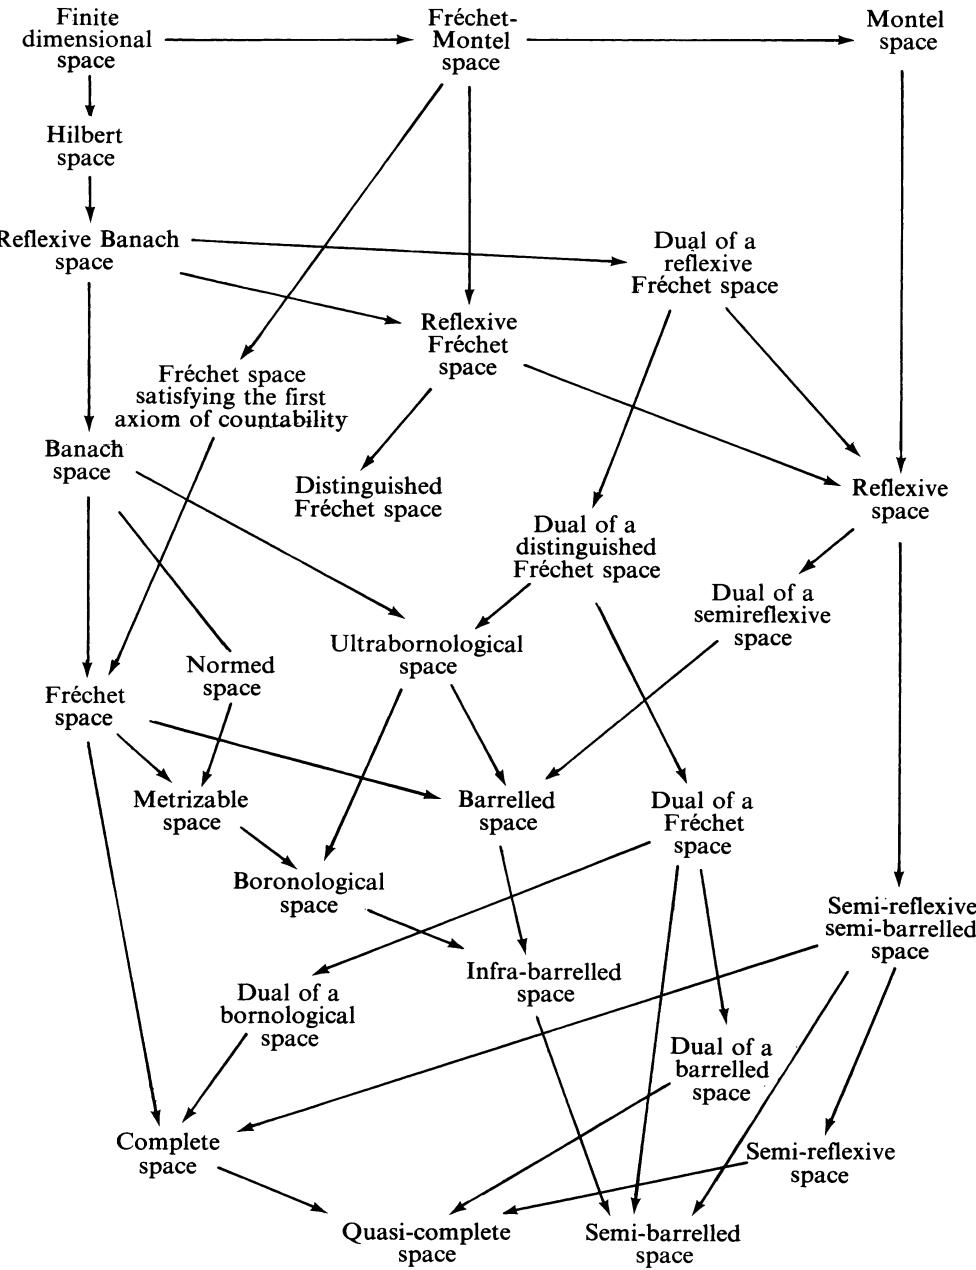
\includegraphics[keepaspectratio]{images/part002_27b26067.jpg}}

\bourbakitable{局部凸空间的对偶上的主要有界结构}{}
\pandocbounded{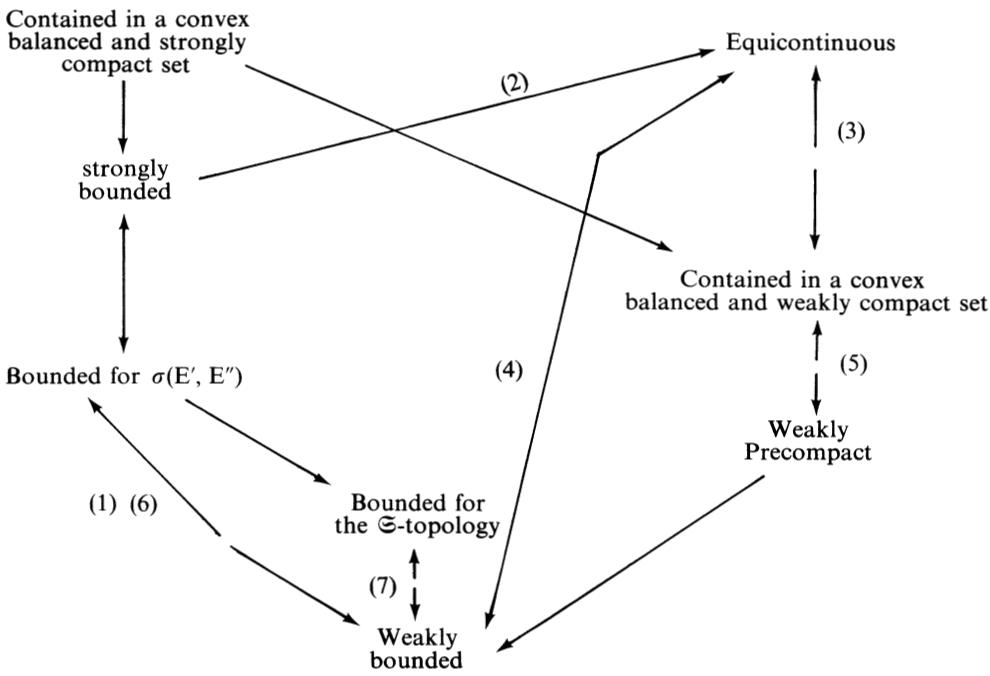
\includegraphics[keepaspectratio]{images/part002_d08e803b.jpg}}

注意 --- 我们用 S 表示 E 的有界子集的这样一个族：其每个元素都含于该族中的某个集合内。箭头旁的数字表示：当同号性质成立时，相应的蕴含关系成立。

\paragraph{性质}

\begin{enumerate}
\def\labelenumi{\arabic{enumi})}
\item
  每当 E 半自反时；
\item
  每当 E 是有界型空间时（III, p.~22, 命题 10）；
\item
  当且仅当 E 具有 Mackey 拓扑 \(\tau(\mathrm{E},\mathrm{E}^{\prime})\) ；
\item
  当且仅当 E 是桶型空间；
\item
  当且仅当 \(\mathbf{E}'\) 对 \(\sigma (\mathbf{E}',\mathbf{E})\) 拟完备
\item
  每当 E 半完备时（更不用说拟完备或完备了）（III, p.~27, 推论 1）；
\item
  每当 \(\mathfrak{S}\) 由闭凸均衡包为半完备的集合组成时（III, p.~27, 定理 2）。
\end{enumerate}

当 E 是 Montel 空间时，上述所有有界结构都相同。

\chapter{\texorpdfstring{希尔伯特空间 \(^{1}\) （初等理论）}{希尔伯特空间 \^{}\{1\} （初等理论）}}

在本章中，K 表示域 R 或域 C。对每个复数 \(\xi = \alpha + i\beta (\alpha, \beta \text{ real}), \overline{\xi}\) 表示共轭 \(\alpha - i\beta\) （\(\xi\) 的）；特别地，\(\overline{\xi} = \xi\) 当且仅当 \(\xi\) 是实数。

\section{准希尔伯特空间与希尔伯特空间}

\subsection{埃尔米特型}

我们回顾《代数》中给出的下述定义（A, IX, § 3, No.~1）：

定义 1. --- 设 E 为域 K 上的向量空间。E 上的（左）埃尔米特型是从 E × E 到 K 中的一个映射 f，它满足下述条件（对 E 中的 \(x_{1}\) 、 \(x_{2}\) 、x、\(y_{1}\) 、 \(y_{2}\) 、y 与 K 中的 \(\lambda\) 、 \(\mu\) ）：

\begin{enumerate}
\def\labelenumi{(\arabic{enumi})}
\tightlist
\item
\item
\end{enumerate}

\[
\begin{array}{c} \left\{ \begin{array}{l} f (x _ {1} + x _ {2}, y) = f (x _ {1}, y) + f (x _ {2}, y) \\ f (x, y _ {1} + y _ {2}) = f (x, y _ {1}) + f (x, y _ {2}) \end{array} \right. \\ \left\{ \begin{array}{l} f (\lambda x, y) = \overline {{\lambda}} f (x, y) \\ f (x, \mu y) = \mu f (x, y) \\ f (x, y) = \overline {{f (y , x)}}  . \end{array} \right. \end{array}\tag{3}
\]

当域 K 是 R 时，E 上的埃尔米特型的概念就化为 \(E \times E\) 上的对称双线性型的概念（A, III, § 6, No.~3）。

我们注意到，条件 (1) 中的第二个与条件 (2) 中的第二个可由其余三个推出。

由 (1) 与 (2) 我们立即得到

\[
f \left(\sum_ {j} \lambda_ {j} x _ {j}, \sum_ {k} \mu_ {k} y _ {k}\right) = \sum_ {j, k} \bar {\lambda} _ {j} \mu_ {k} f \left(x _ {j}, y _ {k}\right).\tag{4}
\]

特别地，若 \(\mathbf{E}\) 是有限维的，且 \((e_j)_{1 \leqslant j \leqslant n}\) 是 \(\mathbf{E}\) 的一个基，则对 \(x = \sum_{j=1}^{n} \xi_j e_j\) 与 \(y = \sum_{j=1}^{n} \eta_j e_j\) ，有

\[
f (x, y) = \sum_ {j, k} \alpha_ {j k} \overline {{{{\xi}}}} _ {j} \eta_ {k}
\]

其中记 \(\alpha_{jk} = f(e_j, e_k)\) ；此外，关系式 (3) 等价于 \(\alpha_{jk} = \overline{\alpha_{kj}}\) 对每对指标 \(j, k\) 成立；这特别蕴含诸数 \(\alpha_{jj}\) 是实数。

由 (3)，数 \(Q(x) = f(x, x)\) 对所有 \(x \in E\) 是实数。此外，我们立即可以建立下列公式，称为极化公式

\begin{enumerate}
\def\labelenumi{(\arabic{enumi})}
\setcounter{enumi}{4}
\tightlist
\item
\end{enumerate}

\[
4 f (x, y) = \sum_ {\varepsilon^ {2} = 1} \varepsilon \mathrm{Q} (x + \varepsilon y) \quad \text { if } \quad \mathbf {K} = \mathbf {R},\tag{6}
\]

\[
4 f (x, y) = \sum_ {\varepsilon^ {4} = 1, \varepsilon \in \mathbf {C}} \varepsilon \mathrm{Q} (x + \overline {{{\varepsilon}}} y) \quad \text { if } \quad \mathbf {K} = \mathbf {C}.
\]

注. --- 我们指出，公式 (6) 对 \(E \times E\) 上的每个半双线性型都成立（也就是说，对每个满足 (1) 与 (2) 但不必满足 (3) 的函数 f 成立）。这个注表明，当 K = C 时，使 \(f(x, x)\) 对所有 \(x \in E\) 为实数的半双线性型 f 必是埃尔米特的：这时关系式 (6) 给出 \(\overline{f(y, x)} = f(x, y)\) ，因为我们有 \(y + \varepsilon x = \varepsilon(x + \overline{\varepsilon}y)\) ，且 \(\mathbf{Q}(\varepsilon z) = \mathbf{Q}(z)\) 对 \(\varepsilon^{4} = 1\) 成立。

由极化公式，我们特别有

命题 1. --- 若 \(f\) 是 \(\mathbf{E}\) 上的埃尔米特型，且 \(\mathbf{M}\) 是 \(\mathbf{E}\) 的一个使 \(f(x, x) = 0\) 对所有 \(x \in \mathbf{M}\) 成立的向量子空间，则也有 \(f(x, y) = 0\) 对每对点 \(x, y\) （\(\mathbf{M}\) 中的）成立。

设 \(f\) 为 \(\mathbf{E}\) 上的埃尔米特型；集 \(\mathbf{N}\) —— 即全体 \(x \in \mathbf{E}\) ，使 \(f(x, y) = 0\) 对所有 \(y \in \mathbf{E}\) 成立 —— 是 \(\mathbf{E}\) 的一个向量子空间。由 (3) 可知，若 \(x_1 \equiv x_2 \pmod{\mathbf{N}}\) 且 \(y_1 \equiv y_2 \pmod{\mathbf{N}}\) ，则有 \(f(x_1, y_1) = f(x_2, y_2)\) ；因此，在商空间 \(\mathrm{E/N}\) 上，我们定义一个半双线性型 \(f\) ，即令 \(\dot{f}(\dot{x}, \dot{y}) = f(x, y)\) （对所有 \(x \in \dot{x}\) 与所有 \(y \in \dot{y}\) ）；显然 \(\dot{f}\) 是埃尔米特的，且关系 \(\langle \dot{f}(\dot{x}, \dot{y}) = 0 \text{ 对所有 } \dot{y} \in \mathrm{E/N} \rangle\) 蕴含 \(\dot{x} = 0 \text{ 于 } \mathrm{E/N}\) ，换言之（A, IX），\(\dot{f}\) 是非退化的。我们说 \(f\) 是与 \(f\) 相伴的非退化埃尔米特型。

\subsection{正埃尔米特型}

定义 2. --- 设 E 为域 K 上的向量空间。E 上的埃尔米特型 f 称为正的，如果 \(f(x, x) \geqslant 0\) 对所有 \(x \in E\) 成立。

显然，向量空间 E 上的全体埃尔米特型构成域 R 上的一个向量空间（当 K 是 C 时，不构成域 C 上的向量空间）：在这个空间中，由定义 2 与命题 1，诸正埃尔米特型构成一个真尖凸锥（II, p.~10）。

命题 2. --- 若 \(f\) 是正埃尔米特型，则有

\[
\left| f (x, y) \right| ^ {2} \leqslant f (x, x) f (y, y)\tag{7}
\]

对 E 中每个 x 与 y（Cauchy-Schwarz 不等式）。

先设 \(f(y, y) \neq 0\) 。对每个 \(\xi \in \mathbf{K}\) ，有

\[
f (y, y) f (x + \xi y, x + \xi y) \geqslant 0
\]

它可写成

\[
f (x, x) f (y, y) - | f (x, y) | ^ {2} + (\xi f (y, y) + \overline {{f (x , y)}}) (\bar {\xi} f (y, y) + f (x, y)) \geqslant 0.
\]

在这个不等式中把 \(\xi\) 换成 \(-\overline{f(x,y)} / f(y,y)\) ，即得 (7)。若 \(f(x,x)\neq 0\) ，论证类似。

最后，若 \(f(x, x) = f(y, y) = 0\) ，则 \(f(x + \xi y, x + \xi y) \geqslant 0\) 对所有 \(\xi \in \mathbf{K}\) 成立，这可写成

\[
\xi f (x, y) + \overline {{{{\xi f (x , y)}}}} \geqslant 0.
\]

在这个不等式中把 \(\xi\) 换成 \(-\overline{f(x,y)}\) ，得 \(-2|f(x,y)|^2 \geqslant 0\) ，从而 \(f(x,y) = 0\) ；在此情形我们同样得到 (7)。

推论 1. --- 若 \(f\) 是正埃尔米特型，则集 \(\mathbf{N}\) —— 即全体 \(x \in \mathbf{E}\) ，使 \(f(x, x) = 0\) —— 与全体 \(x \in \mathbf{E}\) （使 \(f(x, y) = 0\) 对所有 \(y \in \mathbf{E}\) 成立的）组成的向量子空间重合。

推论 2. --- 为使一个正埃尔米特型非退化，必要且充分的是关系 \(x \neq 0\) 蕴含 \(f(x, x) > 0\) 。

这由推论 1 立即得出。

对 E 上的每个正埃尔米特型 f，与 \(f(\mathrm{V}, \mathrm{p.~2})\) 相伴的非退化埃尔米特型显然是 E/N 上的正埃尔米特型。

命题 3. --- 设 f 为 E 上的正埃尔米特型。令

\[
p (x) = f (x, x) ^ {1 / 2}
\]

对所有 \(x \in \mathbb{E}\) 。则 \(p\) 是 \(\mathbb{E}\) 上的半范数，且是范数当且仅当 \(f\) 非退化。只需证明不等式 \(p(x + y) \leqslant p(x) + p(y)\) 。但我们有

\[
f (x + y, x + y) = f (x, x) + f (y, y) + f (x, y) + \overline {{f (x , y)}}
\]

且由 Cauchy-Schwarz 不等式

\[
\begin{array}{c} f (x + y, x + y) \leqslant f (x, x) + f (y, y) + 2 (f (x, x) f (y, y)) ^ {1 / 2} \\ = \bigl (f (x, x) ^ {1 / 2} + f (y, y) ^ {1 / 2} \bigr) ^ {2}. \end{array}\tag{8}
\]

注. --- 1) 假设 \(f\) 是正的且非退化的，并设 \(x, y\) 是两个 \(\neq 0\) 的向量。Cauchy-Schwarz 不等式的证明表明，若 (7) 的两端相等，则存在标量 \(\xi\) 使 \(f(x + \xi y, x + \xi y) = 0\) ，从而 \(x + \xi y = 0\) ，换言之，x 与 y 线性相关；反之是直接的。不等式 (8) 的证明表明，等式 \(p(x + y) = p(x) + p(y)\) 只当 x 与 y 线性相关时才可能成立；若 \(y = \lambda x\) ，前述等式可写成 \(|1 + \lambda| = 1 + |\lambda|\) ，它蕴含 \(\lambda\) 是实数且是正的。

\begin{enumerate}
\def\labelenumi{\arabic{enumi})}
\setcounter{enumi}{1}
\tightlist
\item
  设 \(f\) 为 \(\mathbf{E}\) 上的正埃尔米特型，并给 \(\mathbf{E}\) 赋以半范数 \(x \mapsto f(x, x)^{1/2}\) ；若 \(\dot{f}\) 是定义在 \(\mathrm{E/N}\) 上的与 \(f\) 相伴的正的非退化埃尔米特型，则把范数 \(x \mapsto \hat{f}(\dot{x}, \dot{x})^{1/2}\) 赋予 \(\mathrm{E/N}\) 所得的赋范空间就是与 \(\mathbf{E}\) 相伴的赋范空间（II, p.~5）。
\end{enumerate}

定义 3. --- 设 E 为域 K 上的向量空间。E 上的半范数 p 称为准希尔伯特的，如果存在 E 上的正埃尔米特型 f，使 \(p(x) = f(x, x)^{1/2}\) 对所有 \(x \in E\) 成立。

注意，对 E 上的半范数 p，至多存在一个正埃尔米特型 f，使 \(p(x) = f(x, x)^{1/2}\) 对所有 \(x \in E\) 成立；这由极化公式得出（V, p.~2）。

\subsection{准希尔伯特空间}

定义 4. --- 准希尔伯特空间是一个赋有域 K 上的向量空间结构和一个正埃尔米特型的集合 E。当 K 是 R（相应地，K 是 C）时，我们说 E 是实（相应地，复）准希尔伯特空间。

例. --- 1) 型 \((\lambda, \mu) \mapsto \overline{\lambda}\mu\) 在 K 上定义了一个准希尔伯特结构，称为典范结构。当把 K 看作准希尔伯特空间时，除非另有说明，我们总指它具有这个结构。

\begin{enumerate}
\def\labelenumi{\arabic{enumi})}
\setcounter{enumi}{1}
\tightlist
\item
  设 I 为 R 中的一个区间（有界或无界），E 为定义在 I 上、取值于 C 且具有紧支撑的受控函数（FVR, II, p.~4）组成的集。显然
\end{enumerate}

\(\mathbf{E}\) 是 \(\mathbf{C}\) 上的向量空间；设 \(f\) 为半双线性型 \((x, y) \mapsto \int_{1}^{\infty} \overline{x(t)} y(t) dt\) ；

立即可以看出 \(f\) 是 \(E\) 上的正埃尔米特型，从而在此空间上定义了一个准希尔伯特结构。

\begin{enumerate}
\def\labelenumi{\arabic{enumi})}
\setcounter{enumi}{2}
\tightlist
\item
  设 \(n \geqslant 0\) 为整数。我们在空间 \(\mathbf{K}^n\) 上借助埃尔米特型
\end{enumerate}

\[
(x, y) \mapsto \sum_ {j = 1} ^ {n} \overline {{{{x}}}} _ {j} y _ {j}
\]

定义一个准希尔伯特空间结构（对 \(x = (x_{1}, \ldots, x_{n})\) 与 \(y = (y_{1}, \ldots, y_{n})\) ）。当 \(\mathbf{K}\) 是 \(\mathbf{R}\) 时，我们看到这正是 \(\mathbf{R}^{n}\) 中两个向量的内积（GT, VI, § 2, No.~2）。

* 4) 设 \(\ell^2\) （或 \(\ell^2(\mathbf{N})\) ）为序列 \(x = (x_n)_{n \in \mathbb{N}}\) （元素在 \(\mathbf{K}\) 中且使 \(\sum_{n=0}^{\infty} |x_n|^2\) 为有限）组成的集。可以证明 \(\ell^2\) 是 \(\mathbf{K}^{\mathbf{N}}\) 的向量子空间，并可在其上定义一个准

希尔伯特空间结构于 \(\ell^2\) ，借助埃尔米特型 \((x, y) \mapsto \sum_{n=0}^{\infty} \overline{x}_n y_n\) （参见~V, p.~18）。

\begin{enumerate}
\def\labelenumi{\arabic{enumi})}
\setcounter{enumi}{4}
\tightlist
\item
  设 \(\mathbf{E}\) 为实准希尔伯特空间，\(f\) 为 \(\mathbf{E}\) 上相应的对称双线性型。设 \(\mathrm{E}_{(\mathbf{C})}\) 为 \(\mathbf{E}\) 的向量空间复化；把 \(\mathbf{E}\) 等同于 \(\mathrm{E}_{(\mathbf{C})}\) 的一个子集（借助映射 \(x \mapsto 1 \otimes x\) ），使 \(\mathrm{E}_{(\mathbf{C})}\) 的每个元素都可唯一地写成 \(x_1 + ix_2\) ，其中 \(x_1, x_2\) 属于 \(\mathbf{E}\) 。映射 \(f\) 唯一地延拓为一个埃尔米特型 \(f_{(\mathbf{C})}\) （\(\mathrm{E}_{(\mathbf{C})}\) 上的）；我们有，
\end{enumerate}

\[
f _ {(\mathbf {C})} \left(x _ {1} + i x _ {2}, y _ {1} + i y _ {2}\right) = f \left(x _ {1}, y _ {1}\right) + f \left(x _ {2}, y _ {2}\right) + i \left(f \left(x _ {1}, y _ {2}\right) - f \left(x _ {2}, y _ {1}\right)\right).
\]

特别地，我们有

\[
f _ {(\mathbf {C})} (x _ {1} + i x _ {2}, x _ {1} + i x _ {2}) = f (x _ {1}, x _ {1}) + f (x _ {2}, x _ {2}) \geqslant 0,
\]

因此 \(f_{(\mathbf{C})}\) 是正的。我们说 \(\mathrm{E}_{(\mathbf{C})}\) （赋有 \(f_{(\mathbf{C})}\) ）是 \(\mathbf{E}\) 的准希尔伯特空间复化。

每当只考虑向量空间 E 上的一个准希尔伯特空间结构时，对 E 的一对点 \((x, y)\) ，定义该结构的埃尔米特型在这对点上的值记作 \(\langle x|y\rangle_{E}\) ，或在不致混淆时简记为 \(\langle x|y\rangle\) 。这个数称为 x 与 y 的内积 \(^{1}\) （当 y = x 时称为 x 的标量平方）。向量 x, y 称为正交的，如果 \(\langle x|y\rangle = 0\) 。函数 \(x \mapsto \|x\| = \langle x|x\rangle^{1/2}\) 是向量空间 E 上的半范数（V, p.~3）；准希尔伯特空间总是被认为赋有这个半范数（从而也赋有相应的拓扑与一致结构）。

采用这些记号，在准希尔伯特空间 E 中，Cauchy-Schwarz 不等式可写成

\[
\left| \langle x | y \rangle \right| \leqslant \| x \|\cdot \| y \|.\tag{9}
\]

因此，内积是 \(\mathbf{E} \times \mathbf{E}\) 上的连续半双线性型（II, p.~5, 命题 4）。

为使 E 是 Hausdorff 的，必要且充分的是 \(x \mapsto \|x\|\) 是 E 上的范数；换言之，埃尔米特型 \((x, y) \mapsto \langle x | y \rangle\) 是正的且非退化的；这等价于说 0 是 E 中唯一与自身正交的向量。

按照一般定义（S, IV, § 1, No.~5），准希尔伯特空间 E 到准希尔伯特空间 F 上的同构是从 E 到 F 上的一个双射线性映射 u，它满足

\[
\langle u (x) | u (y) \rangle = \langle x | y \rangle\tag{10}
\]

对 E 中每个 x 与 y。由此推出，\(\|u(x)\| = \|x\|\) 对所有 \(x \in E\) 成立，且 u 显然是 E 与 F 的拓扑向量空间结构之间的同构；若 E 与 F 是 Hausdorff 的，则 u 是 E 到 F 上的一个等距。反之，若 u 是从 E 到 F 上的双射线性映射，且 \(\|u(x)\| = \|x\|\) 对所有 \(x \in E\) 成立，则极化公式（V, p.~2）表明 u 是 E 到 F 上的准希尔伯特空间同构。

设 \(E\) 为复准希尔伯特空间，\(\langle x|y\rangle\) 为 \(E\) 中的内积。在集合 \(E\) 上，可以定义关于 \(C\) 的第二个向量空间结构，取同样的加法群规律，并以 \((\lambda, x) \mapsto \overline{\lambda}x\) 为外合成规律（A, II, § 1, No.~13）；对这个向量空间结构，\((x, y) \mapsto \langle y|x\rangle\) 是一个正埃尔米特

\(^{1}\) 有时我们会用 \((x|y)\) 表示 \(\langle y|x\rangle\) 。注意 V, p.~2 的公式 (4) 取下列等价形式：

(4')

\[
\langle \sum_ {i} \lambda_ {i} x _ {i} | \sum_ {j} \mu_ {j} y _ {j} \rangle = \sum_ {i, j} \overline {{{{\lambda}}}} _ {i} \mu_ {j} \langle x _ {i} | y _ {j} \rangle .\tag{4"}
\]

\[
(\sum_ {i} \lambda_ {i} x _ {i} | \sum_ {j} \mu_ {j} y _ {j}) = \sum_ {i, j} \lambda_ {i} \overline {{\mu}} _ {j} (x _ {i} | y _ {j}).
\]

型。给 E 赋以这个新的向量空间结构与新的埃尔米特型所得的准希尔伯特空间 \(\overline{E}\) 称为 E 的共轭空间。E 到 \(\overline{E}\) 上的同构 u 是 E 到自身的一个半线性映射（关于 C 的自同构 \(\xi \mapsto \overline{\xi}\) ），满足 \(\langle u(y)|u(x)\rangle = \langle x|y\rangle\) 或 \(\langle u(x)|u(y)\rangle = \overline{\langle x|y\rangle}\) （对 E 中的 x, y）；这样的映射称为准希尔伯特空间 E 的半自同构。

若 E 是准希尔伯特空间，M 是 E 的向量子空间，则内积 \(\langle x|y\rangle\) 在 \(M \times M\) 上的限制是 M 上的正埃尔米特型，从而在 M 上定义了一个准希尔伯特空间结构；我们说这个结构由 E 的结构诱导，或说 M 是 E 的准希尔伯特子空间。

\subsection{希尔伯特空间}

定义 5. --- 希尔伯特空间（或 Hilbert 空间）是 Hausdorff 且完备的准希尔伯特空间。我们说向量空间 E（K 上的）上的范数是希尔伯特的，如果它是准希尔伯特的，且赋范空间 E 是完备的。

若 E 是希尔伯特空间且 M 是 E 的闭向量子空间，则 M 上诱导的准希尔伯特空间结构实际上是希尔伯特空间结构。这时我们说赋有诱导结构的 M 是 E 的希尔伯特子空间。

例. --- 1) V, p.~4 的例 1、3、4 中定义的准希尔伯特空间都是希尔伯特空间。另一方面，例 2 中定义的准希尔伯特空间既非 Hausdorff，也非完备。希尔伯特空间的复化是希尔伯特空间。

* 2) 设 X 为 Hausdorff 拓扑空间，\(\mu\) 为 X 上的正测度。设 \(L^2(X, \mu)\) 为 X 上取值于 C 的全体平方 \(\mu\) -可积函数按 \(\mu\) 的等价类组成的空间。这是一个复希尔伯特空间，其内积由下式给出

\[
\langle f | g \rangle = \int_ {\mathrm{X}} \overline {{{f (x)}}} g (x) d \mu (x). *
\]

* 3) 设 \(n \geqslant 1\) 为整数，\(U\) 为 \(\mathbf{R}^n\) 中的开集。设 \(\mu\) 为 \(U\) 上由 \(\mathbf{R}^n\) 上的 Lebesgue 测度诱导的测度，令 \(\mathcal{H}^0 = L^2(U, \mu)\) 。用 \(\mathcal{H}^1\) 表示具有下列性质的所有函数 \(f \in \mathcal{H}^0\) 组成的空间；对 \(1 \leqslant i \leqslant n\) ，存在函数 \(g_i \in \mathcal{H}^0\) 使

\[
\int_ {\mathrm{U}} g _ {i} (x) h (x) d \mu (x) = - \int_ {\mathrm{U}} f (x) \mathrm{D} _ {i} h (x) d \mu (x)
\]

对每个函数 \(h\) （\(\mathbf{C}^1\) 类的，在 \(\mathbf{U}\) 中有紧支撑的）成立。函数 \(g_i\) 在相差一个关于 \(\mu\) 的等价类的意义下唯一确定，记作 \(\mathbf{D}_i f\) 或 \(\partial f / \partial x_i\) （第 i 个偏导数）。对整数 \(s \geqslant 1\) 用归纳法，把 \(\mathcal{H}^s\) 定义为所有函数 \(f \in \mathcal{H}^1\) （使 \(D_i f \in \mathcal{H}^{s-1}\) 对 \(1 \leqslant i \leqslant n\) 成立的）组成的集。我们用下列公式在 \(\mathcal{H}^s\) 上定义内积

\[
\langle f | g \rangle = \sum_ {k = 0} ^ {s} \sum_ {1 \leqslant i _ {1} \leqslant \dots \leqslant i _ {k} \leqslant n} \int \overline {{{{\mathrm{D} _ {i _ {1}} \dots \mathrm{D} _ {i _ {k}} f}}}}. \mathrm{D} _ {i _ {1}} \dots \mathrm{D} _ {i _ {k}} g d \mu .
\]

于是 \(\mathcal{H}^s\) 是一个复希尔伯特空间，称为指标 \(s\) 的 Sobolev 空间。

* 4) 设 X 为 \(\mathbf{C}^r\) 类（\(r \geqslant 1\) ）纯的、维数有限为 \(n\) 的微分流形。

在向量纤维空间 \(\Lambda^{n}\mathrm{T}(\mathrm{X})\) 中，设 L 为零截面的余集。对每个实数 \(\lambda \neq 0\) ，映射 \(u \mapsto \lambda u\) （从 \(\Lambda^{n}\mathrm{T}(\mathrm{X})\) 到自身的）使 L 稳定。

设 \(\alpha\) 为复数。一个复值函数 \(\omega\) （定义在 \(\mathbf{L}\) 上），若 \(\omega (\lambda u) = |\lambda |^{\alpha}\omega (u)\) 对 \(u\in \mathbf{L}\) 与任意非零实数 \(\lambda\) 成立，就称为 \(\alpha\) 阶密度（\(\mathbf{X}\) 上的）。我们说 1 阶密度 \(\omega\) 是局部可积的，如果存在一个开覆盖 \((\mathrm{U}_i)_{i\in \mathbf{I}}\) （\(\mathbf{X}\) 的），且对每个 \(i\in \mathbf{I}\) ，存在一个坐标系 \(\xi_i = (\xi_i^1,\dots,\xi_i^n)\) （\(\mathrm{U}_i\) 上的）与一个复值函数 \(f_{i}\) （\(\xi_i(\mathrm{U}_i)\) 上的），满足下列条件：a) 函数 \(f_{i}\) 在开集 \(\xi_i(\mathrm{U}_i)\) （\(\mathbf{R}^n\) 中的）上关于 Lebesgue 测度 \(\mu\) 是局部可积的；

\begin{enumerate}
\def\labelenumi{\alph{enumi})}
\setcounter{enumi}{1}
\tightlist
\item
  设 \(x \in \mathbf{U}_i\) ；若 \((\partial_{1,i,x}, \ldots, \partial_{n,i,x})\) 是 \(\mathrm{T}_x\mathrm{X}\) 的、与坐标系 \((\xi_i^1, \ldots, \xi_i^n)\) （\(\mathbf{U}_i\) 中的）相伴的基，则有
\end{enumerate}

\[
\omega \left(\partial_ {1, i, x} \wedge \dots \wedge \partial_ {n, i, x}\right) = f _ {i} \left(\xi_ {i} ^ {1} (x), \dots , \xi_ {i} ^ {n} (x)\right).
\]

于是，存在唯一的测度 \(\tilde{\omega}\) （\(\mathbf{X}\) 上的），使对每个 \(i\in \mathrm{I}\) ，在 \(\xi_{i}\) 下 \(\tilde{\omega}\) 在 \(\mathrm{U}_i\) 上的限制的像等于测度 \(f_{i}.\mu\) （参见~VAR, R, 10.4.3）。

设 \(\mathcal{V}\) （相应地，\(\mathcal{N}\) ）为由可测密度 \(\omega\) （\(1/2\) 阶）组成的、使与 1 阶密度 \(|\omega|^2\) 相伴的测度有界（相应地，为零）的向量空间。设 \(\omega_1\) 与 \(\omega_2\) 属于 \(\mathcal{V}\) ；则 \(\omega = \overline{\omega}_1\omega_2\) 是 1 阶密度，且测度 \(\tilde{\omega}\) （与 \(\omega\) 相伴的）有界；数 \(\int_{\mathbf{X}}\tilde{\omega}\) 只依赖于类 \(\dot{\omega}_1\) 与 \(\dot{\omega}_2\) （即 \(\omega_1\) 与 \(\omega_2\) 模 \(\mathcal{N}\) 的类），记作 \(\langle\omega_1|\omega_2\rangle\) 或 \(\langle\dot{\omega}_1|\dot{\omega}_2\rangle\) 。于是映射 \((\dot{\omega}_1,\dot{\omega}_2)\mapsto\langle\dot{\omega}_1|\dot{\omega}_2\rangle\) 给向量空间 \(\Omega_{1/2}(\mathbf{X})=\mathcal{V}/\mathcal{N}_{*}\) 赋以一个复希尔伯特空间结构。

*5) 设 D 为 C 中以 0 为心、1 为半径的开圆盘。Hardy 空间 \(\mathrm{H}^2 (\mathbf{D})\) 由满足下列条件的全纯函数 \(f\colon \mathbf{D}\to \mathbf{C}\) 组成：

\[
\sup _ {0 <   \mathbf {R} <   1} \int_ {0} ^ {1} | f (\mathbf {R}. \mathbf {e} (\theta)) | ^ {2} d \theta <   + \infty .
\]

若 \(f_{1}\) 与 \(f_{2}\) 属于 \(\mathrm{H}^2 (\mathbf{D})\) ，则极限

\[
\langle f _ {1} | f _ {2} \rangle = \lim _ {\mathbf {R} \rightarrow 1} \int_ {0} ^ {1} \overline {{{f _ {1} (\mathbf {R} . \mathbf {e} (\theta))}}}. f _ {2} (\mathbf {R}. \mathbf {e} (\theta)) d \theta
\]

存在；映射 \((f_1, f_2) \mapsto \langle f_1 | f_2 \rangle\) 给向量空间 \(\mathbf{H}^2(\mathbf{D})\) 赋以一个复希尔伯特空间结构。

为使函数 \(f: \mathbf{D} \to \mathbf{C}\) 属于 \(\mathbf{H}^2(\mathbf{D})\) ，必要且充分的是存在复数的序列 \((a_n)_{n \in \mathbb{N}}\) ，使 \(\sum_{n=0}^{\infty} |a_n|^2 < +\infty\) 且

\[
f (z) = \sum_ {n = 0} ^ {\infty} a _ {n} z ^ {n}
\]

对所有 \(z \in \mathbf{D}\) 成立。这时有 \(\| f\|^2 = \sum_{n=0}^{\infty} |a_n|^2\) ，由此给出从 \(\mathrm{H}^2(\mathrm{D})\) 到希尔伯特空间 \(\ell^2\) 上的一个同构（V, p.~4）。 *

每个 Hausdorff 准希尔伯特空间都同构于一个在相差一个同构的意义下确定的希尔伯特空间的处处稠密子空间。确切地说：

命题 4. --- 设 E 为 Hausdorff 准希尔伯特空间，\(\hat{E}\) 为 E 的赋范空间完备化（GT, IX, § 3, No.~3）。内积 \((x, y) \mapsto \langle x|y \rangle\) 由连续性延拓为 \(\hat{\mathbf{E}}\) 上的正且非退化的埃尔米特型，并在 \(\hat{\mathbf{E}}\) 上定义一个希尔伯特空间结构。

\((x, y) \mapsto \langle x|y \rangle\) 到 \(\hat{E} \times \hat{E}\) 上的延拓的存在性由这个半双线性型在 \(E \times E\) 上的连续性得出（GT, III, §6, No.~5, 定理 1）。此外，这个延拓（仍记作 \((x, y) \mapsto \langle x|y \rangle\) ）是埃尔米特型且满足关系 \(\langle x|x\rangle = \|x\|^2\) ，这由恒等式延拓原理得出（ \(\|x\|\) 是 \(\hat{E}\) 上把 E 上的范数用连续性延拓所得的范数）；这就证明了关系 \(\langle x|x\rangle = 0\) 蕴含在 \(\hat{E}\) 中 x = 0，从而型 \((x, y) \mapsto \langle x|y \rangle\) 是正的且非退化的，于是在 \(\hat{E}\) 上定义一个希尔伯特空间结构。

证毕。

这个希尔伯特空间称为 Hausdorff 准希尔伯特空间 E 的完备化。

* 例 6. --- 设 U 为 \(\mathbf{R}^n\) 的开子集（ \(n \geqslant 1\) ）。设 \(\mathcal{C}_0^1(\mathrm{U})\) 为 U 中具有紧支撑的 \(\mathbf{C}^1\) 类函数全体组成的向量空间。我们在 \(\mathcal{C}_0^1(\mathrm{U})\) 上定义一个 Hausdorff 准希尔伯特空间结构，其内积由下式给出

\[
\langle f | g \rangle = \sum_ {i = 1} ^ {n} \int_ {\mathrm{U}} \overline {{{{\mathbf {D} _ {i} f (x)}}}}. \mathbf {D} _ {i} g (x) d x.
\]

这个准希尔伯特空间不完备。它的完备化称为与 U 相伴的 Dirichlet 空间。 *

推论. --- 设 V 为 K 上的向量空间，f 为 V 上的正埃尔米特型。a) 存在一个 Hilbert 空间 E 和一个线性映射 \(u:V \rightarrow E\) ，使 \(f(x,y) = \langle u(x)|u(y) \rangle\) 对 V 中的 x, y 成立，且使 \(u(V)\) 在 E 中稠密。

\begin{enumerate}
\def\labelenumi{\alph{enumi})}
\setcounter{enumi}{1}
\tightlist
\item
  若两个偶 \((\mathbf{E}_{i}, u_{i})\) 满足与 a) 类似的条件，则存在唯一的同构 \(\phi\) （从 Hilbert 空间 \(E_{1}\) 到 Hilbert 空间 \(E_{2}\) 上的）使 \(u_{2} = \phi \circ u_{1}\) 。
\end{enumerate}

设 N 为全体 \(x \in V\) （使 \(f(x, x) = 0\) 的）组成的集。我们在空间 V/N 上用 \(\langle \dot{x} | \dot{y} \rangle = f(x, y)\) （对 \(x \in \dot{x}\) 与 \(y \in \dot{y}\) ）定义一个正且非退化的埃尔米特型。设 E 为 V/N 的希尔伯特空间完备化，u 为从 V 到 E 中的映射 \(x \mapsto x + N\) 。于是 a) 的条件满足。

在 b) 的假设下，N 等于 \(u_{1}\) 的核，也等于 \(u_{2}\) 的核。因此存在双射线性映射 \(\phi_{0}\) （从 \(u_{1}(V)\) 到 \(u_{2}(V)\) 上的），使 \(u_{2}(x) = \phi_{0}(u_{1}(x))\) 对所有 \(x \in V\) 成立。立即可以验证 \(\phi_{0}\) 是准希尔伯特空间之间的同构，从而是一个等距。由于对 i = 1, 2，\(u_{i}(V)\) 在 \(E_{i}\) 中稠密，\(\phi_{0}\) 唯一地延拓为一个等距 \(\phi\) （从 \(E_{1}\) 到 \(E_{2}\) 上的），由此得 b)。

我们说希尔伯特空间 \(\mathbf{E}\) 是 \(\mathbf{V}\) 的分离完备化（关于型 \(f\) ）。

例 7. --- 设 G 为一个群（单位元为 1），\(\pi\) 为从 G 到一个复希尔伯特空间 E 的自同构群中的同态；我们说 \(\pi\) 是 G 在 E 中的一个酉表示。设 \(a \in E\) ；我们令

\[
\phi (x) = \langle a | \pi (x). a \rangle
\]

对所有 \(x \in \mathbf{G}\) 成立。则 \(\phi : \mathbf{G} \to \mathbf{C}\) 是正定的，换言之满足关系：

(PD) 对 C 中每个 \(\lambda_{1},\ldots,\lambda_{n}\) 与 G 中每个 \(x_{1},\ldots,x_{n}\) ，有

\[
\sum_ {i, j = 1} ^ {n} \overline {{\lambda}} _ {i} \lambda_ {j} \phi (x _ {i} ^ {- 1} x _ {j}) \geqslant 0.\tag{11}
\]

事实上，(11) 的左端正是 \(\| \sum_{i=1}^{n} \lambda_i \pi(x_i). a \|^2\) 。

反之，设 \(\phi\) 为 \(G\) 上的正定函数。设 \(\mathbf{C}^{(G)}\) 为 \(G\) 上具有有限支撑的全体函数组成的向量空间。我们定义一个埃尔米特型 \(\Phi\) 于 \(G\) 上：

\[
\Phi (u, v) = \sum_ {x, y \in G} \overline {{u (x)}} v (y) \phi (x ^ {- 1} y)\tag{12}
\]

而关系式 (PD) 表明 \(\Phi\) 是正的。由命题 4 的推论，存在一个希尔伯特空间 \(E\) 和一个线性映射 \(\rho : \mathbf{C}^{(G)} \to E\) ，其像稠密，使得

\[
\Phi (u, v) = \langle \rho (u) | \rho (v) \rangle \quad \text { for } \quad u, v \quad \text { in } \quad \mathbf {C} ^ {(G)}.\tag{13}
\]

对每个 \(x \in \mathbf{G}\) ，设 \(\gamma_x\) 为 \(x\) 在 \(\mathbf{C}^{(\mathrm{G})}\) 中的左平移，由 \(\gamma_x u(y) = u(x^{-1}y)\) （对 \(u \in \mathbf{C}^{(\mathrm{G})}\) 与 \(y \in \mathbf{G}\) ）定义。我们有 \(\Phi(\gamma_x u, \gamma_x v) = \Phi(u, v)\) 。现在把命题 4 的推论的断言 \(b\) 应用于 \(\rho\) 与 \(\rho \circ \gamma_x\) ：存在唯一的自同构 \(\pi(x)\) （希尔伯特空间 \(E\) 上的）使 \(\rho \circ \gamma_x = \pi(x) \circ \rho\) 。立即可以看出 \(\pi\) 是从 \(G\) 到 \(E\) 的自同构群中的同态。

设 \(\delta\) 为 \(\mathbf{C}^{(\mathrm{G})}\) 中由 \(\delta(1) = 1\) 与 \(\delta(x) = 0\) （对 \(x \neq 1\) ，\(\mathbf{G}\) 中的）定义的元素。我们有 \(u = \sum_{x \in \mathbf{G}} u(x) \cdot \gamma_x \delta\) 对所有 \(u \in \mathbf{C}^{(\mathrm{G})}\) 成立，于是 \(\rho(u) = \sum_{x \in \mathbf{G}} u(x) \pi(x) \cdot a\) （令 \(a = \rho(\delta)\) ）。公式 (12) 与 (13) 蕴含 \(\phi(x) = \langle a | \pi(x) \cdot a \rangle\) 对所有 \(x \in \mathbf{G}\) 成立。我们注意，向量 \(\pi(x) \cdot a\) （对所有 \(x \in \mathbf{G}\) ）组成的集在 \(\mathbf{E}\) 中是完全的。

\subsection{准希尔伯特空间的凸子集}

若对准希尔伯特空间 E 的任意两点 x, y 计算 \(\|x - y\|^{2} = \langle x - y|x - y \rangle\) 与 \(\|x + y\|^{2} = \langle x + y|x + y \rangle\) ，立即得到«中线恒等式»

\[
\left\| \frac {1}{2} (x + y) \right\| ^ {2} + \left\| \frac {1}{2} (x - y) \right\| ^ {2} = \frac {1}{2} (\| x \| ^ {2} + \| y \| ^ {2}).\tag{14}
\]

由这个恒等式我们导出下列命题：

\pandocbounded{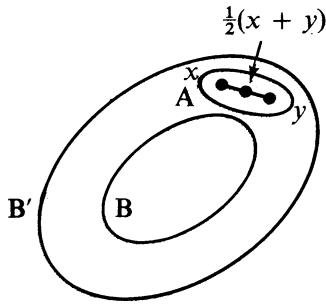
\includegraphics[keepaspectratio]{images/part002_56de9e6b.jpg}}\\
图 1.

命题 5. --- 设 E 为准希尔伯特空间。设 d 为实数 \textgreater0，δ 为使 \(0 \leqslant \delta \leqslant d\) 的实数。设 B 与 B' 为 E 的子集，分别由 \(\|x\| < d\) 与 \(\| x\| \leqslant d + \delta\) 定义，并设 A 为含于 \(\mathbf{B}' - \mathbf{B}\) 的凸集。则对 A 的每对点 \(x, y\) ，有 \(\| x - y\| \leqslant \sqrt{12d\delta}\) （图~1）。

事实上，我们有 \(\frac{1}{2} (x + y)\in \mathbf{A}\) ，故 \(\| \frac{1}{2} (x + y)\| \geqslant d\) ；于是由 (14) 得不等式

\[
\left\| \frac {1}{2} (x - y) \right\| ^ {2} = \frac {1}{2} \left(\| x \| ^ {2} + \| y \| ^ {2}\right) - \left\| \frac {1}{2} (x + y) \right\| ^ {2} \leqslant (d + \delta) ^ {2} - d ^ {2} \leqslant 3 d \delta
\]

由此即得命题。

定理 1. --- 设 E 为准希尔伯特空间，H 为 E 的一个非空凸子集，使得 H 是 E 的 Hausdorff 且完备的一致子空间。对每个 \(x \in E\) ，在 H 中存在唯一的点 \(p_{\mathrm{H}}(x)\) 使 \(\|x - p_{\mathrm{H}}(x)\| = \inf_{y \in \mathrm{H}} \|x - y\|\) 。H 的元素 \(p_{\mathrm{H}}(x)\) 也是 H 中满足关系式 \(^{1}\) 的唯一元素 a

\[
\mathcal {R} \langle x - a | y - a \rangle \leqslant 0\tag{15}
\]

对所有 \(y \in \mathbf{H}\) 成立。

\pandocbounded{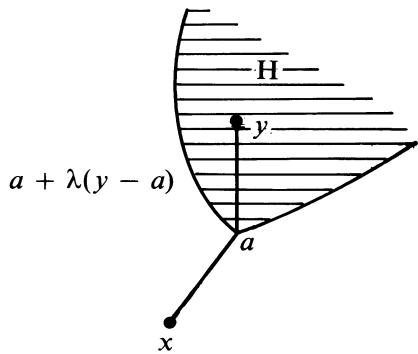
\includegraphics[keepaspectratio]{images/part002_6909685c.jpg}}\\
图 2.

令 \(d = \inf_{y \in \mathbf{H}} \| x - y \|\) ，且对每个整数 \(n > 0\) ，设 \(\mathrm{H}_n\) 为点 \(y\) （在 \(\mathbf{H}\) 中，使 \(\| x - y \| \leqslant d + n^{-1}\) ）所成的集。集 \(\mathrm{H}_n\) 在 \(\mathbf{H}\) 中是闭的，是凸的且非空，且由命题 5，其直径以 \(\sqrt{12d / n}\) 为界（对所有足够大的 \(n\) ）。由于序列 \((\mathrm{H}_n)_{n \geqslant 1}\) 递减，且集 \(\mathbf{H}\) 是 Hausdorff 且完备的，因此 Cauchy 滤子 \((\mathrm{H}_n)_{n \geqslant 1}\) 的基收敛到一点 \(p_{\mathbf{H}}(x)\) （属于 \(\mathbf{H}\) ）；我们有 \(\{p_{\mathbf{H}}(x)\} = \bigcap_{n \geqslant 1} \mathrm{H}_n\) ，故 \(p_{\mathbf{H}}(x)\) 是唯一的点 \(a\) （在 \(\mathbf{H}\) 中），使 \(\| x - a \| = d\) 。

\(^{1}\) 我们回顾（GT, VIII, § 1, No.~1），\(\mathcal{R}(z)\) 表示复数 z 的实部；若 z 是实数，则有 \(\mathcal{R}(z)=z\) 。

设 \(y \in H\) ；由于 \(H\) 是凸的，点 \(z(\lambda) = p_{\mathbf{H}}(x) + \lambda(y - p_{\mathbf{H}}(x))\) （\(E\) 中的）属于 \(H\) ，对每个实数 \(\lambda\) （满足 \(0 < \lambda < 1\) 的）。因此我们有

\[
\left\| x - z (\lambda) \right\| ^ {2} \geqslant \left\| x - p _ {\mathrm{H}} (x) \right\| ^ {2} \quad \text { for } \quad 0 <   \lambda <   1,
\]

由此给出

\[
\mathcal {R} \left\langle x - p _ {\mathrm{H}} (x) \mid y - p _ {\mathrm{H}} (x) \right\rangle = \lim _ {\lambda \rightarrow 0} \frac {1}{2 \lambda} \left\{\| x - p _ {\mathrm{H}} (x) \| ^ {2} - \| x - z (\lambda) \| ^ {2} \right\} \leqslant 0.
\]

反之，设 \(a\) 为 \(\mathbf{H}\) 的一点，使 \(\mathcal{R}\langle x - a|y - a\rangle \leqslant 0\) 对所有 \(y\in \mathbf{H}\) 成立。对每个 \(y\in \mathbf{H}\) ，有

\[
\left\| x - y \right\| ^ {2} = \left\| x - a \right\| ^ {2} + \left\| y - a \right\| ^ {2} - 2 \mathcal {R} \langle x - a | y - a \rangle \geqslant \left\| x - a \right\| ^ {2},
\]

于是 \(\| x - a\| = d\) ，最后由证明的第一部分得出 \(a = p_{\mathrm{H}}(x)\) 。证毕。

在下面，E 到 H 中的映射 \(p_{H}\) 将称为从 E 到 H 上的投影。我们注意 \(p_{\mathrm{H}}(x)=x\) 对所有 \(x\in H\) 成立。

定理 1 的第一部分在关于空间 E 的更一般假设下仍然成立（V, p.~67, 练习 31）。

定理 1 的证明特别建立了下列性质：

推论 1. --- 设 I 为被滤子 \(\mathfrak{F}\) 定向的集合，\((y_i)_{i\in I}\) 为 H 的点的一个族。设 \(x\in E\) 。假设我们有

\[
\lim _ {i, \mathfrak {F}} \| x - y _ {i} \| = \inf _ {z \in \mathrm{H}} \| x - z \|.
\]

则 \(y_{i}\) 趋于 \(p_{\mathrm{H}}(x)\) （关于滤子 \(\mathfrak{F}\) ）。

推论 2. --- 对 E 中每个 x, y，有

\[
\left\| p _ {\mathrm{H}} (x) - p _ {\mathrm{H}} (y) \right\| \leqslant \left\| x - y \right\|.
\]

特别地，从 E 到 H 中的映射 \(p_{H}\) 是连续的。

设 \(x, y\) 为 \(E\) 的两点。令 \(a = p_{\mathrm{H}}(x) - x\) ，\(b = p_{\mathrm{H}}(y) - p_{\mathrm{H}}(x)\) ，\(c = y - p_{\mathrm{H}}(y)\) 。由公式 (15)（V, p.~10）我们有 \(\mathcal{R}\langle a|b\rangle \geqslant 0\) 与 \(\mathcal{R}\langle c|b\rangle \geqslant 0\) 。我们还有 \(a + b + c = y - x\) ，由此给出

\[
\| x - y \| ^ {2} = \| a + b + c \| ^ {2} = \| b \| ^ {2} + \| a + c \| ^ {2} + 2 \mathscr {R} \langle a | b \rangle + 2 \mathscr {R} \langle c | b \rangle
\]

\[
\geqslant \| b \| ^ {2} = \left\| p _ {\mathrm{H}} (x) - p _ {\mathrm{H}} (y) \right\| ^ {2}.
\]

这就证明了推论 2。

命题 6. --- 设 E 为准希尔伯特空间，\(\Phi\) 为由 E 的非空、Hausdorff 且完备的凸子集组成的非空递减有向集。对每个 \(x \in \mathrm{E}\) 与 E 的每个子集 H，令 \(d(x, \mathrm{H}) = \inf_{z \in \mathrm{H}} \| x - z \|\) 。为使属于 \(\Phi\) 的诸集 H 的交 M 非空，必要且充分的是存在 E 中的 \(x_0\) 使 \(\sup_{\mathbf{H} \in \Phi} d(x_0, \mathbf{H})\) 有限。这时对每个 \(x \in \mathbf{E}\) 我们有

\(p_{\mathbf{M}}(x) = \lim_{\mathrm{H}\in \Phi}p_{\mathrm{H}}(x)\) （关于有向集 \(\Phi\) 的极限）。

若 \(\mathbf{M}\) 非空，则 \(d(x,\mathrm{H})\leqslant d(x,\mathbf{M})\) 对所有 \(\mathbf{H}\in \Phi\) 与所有 \(x\in \mathbb{E}\) 成立。

反之，假设存在一点 \(x_0\) （在 \(\mathbf{E}\) 中）与实数 \(\mathbf{C} \geqslant 0\) ，使 \(d(x_0, \mathbf{H}) \leqslant \mathbf{C}\) 对所有 \(\mathbf{H} \in \Phi\) 成立。设 \(x \in \mathbf{E}\) ；则

\[
d (x, \mathrm{H}) \leqslant \| x - x _ {0} \| + \mathrm{C} \quad \text { for   all } \quad \mathrm{H} \in \Phi ,
\]

于是数 \(d = \sup_{\mathbf{H} \in \Phi} d(x, \mathbf{H})\) 有限。设 \(\mathbf{B}\) 为全体 \(z \in E\) （使 \(\| x - z\| \leqslant d\) 的）组成的集。由于 \(\mathbf{B}\) 在 \(\mathbf{E}\) 中是凸的且闭的，故诸集 \(\mathrm{H} \cap \mathrm{B}\) （当 \(\mathrm{H}\) 取遍 \(\Phi\) ）是凸的、Hausdorff 的且完备的。设 \(\varepsilon > 0\) ；存在集 \(\mathrm{H} \in \Phi\) 使 \(d(x, \mathrm{H}) \geqslant \mathrm{d} - \varepsilon\) ，且若 \(\varepsilon < d/2\) ，则 \(\mathrm{H} \cap \mathrm{B}\) 的直径由命题 5（V, p.~9）以 \(\sqrt{12\varepsilon(d - \varepsilon)}\) 为界。换言之，对所有 \(\mathrm{H}_0 \in \Phi\) ，诸闭集 \(\mathrm{H} \cap \mathrm{B}\) （\(\mathrm{H} \in \Phi\) 且 \(\mathrm{H} \subset \mathrm{H}_0\) ）构成 Hausdorff 完备空间 \(\mathrm{H}_0\) 上 Cauchy 滤子的一个基。因此诸集 \(\mathrm{H} \cap \mathrm{B}\) （对 \(\mathrm{H} \in \Phi\) ）的交化为一点 \(y\) 。我们得到 \(y \in \mathbf{M}\) 与 \(\| x - y \| = d = d(x, \mathbf{M})\) 。由于 \(\mathbf{M}\) 在 \(\mathrm{H}_0\) 中是闭的，它是 \(\mathbf{E}\) 中 Hausdorff、凸且完备的集，故 \(y = p_{\mathbf{M}}(x)\) 。对每个 \(\mathrm{H} \in \Phi\) ，我们有 \(p_{\mathrm{H}}(x) \in \mathrm{H} \cap \mathrm{B}\) ，由此得出 \(p_{\mathbf{M}}(x) = \lim_{\mathrm{H} \in \Phi} p_{\mathrm{H}}(x)\) 。

命题 7. --- 设 E 为 Hausdorff 准希尔伯特空间，\(\Psi\) 为由 E 的非空、凸、完备子集组成的非空递增有向集。令 \(A = \bigcup_{H \in \Psi} H\)

并假设闭包 \(\mathbf{N}\) （\(\mathbf{A}\) 的）是完备的。则 \(\mathbf{N}\) 是凸的，且 \(p_{\mathrm{N}}(x) = \lim_{\mathrm{H}\in \Psi}p_{\mathrm{H}}(x)\) 对所有 \(x\in \mathrm{E}\) 成立。

显然 A 是凸的，故其闭包 N 是凸的（II, p.~13）。采用命题 6 的记号，\(d(x, \mathrm{N}) = \inf_{\mathrm{H} \in \Psi} d(x, \mathrm{H})\) ，因此 \(d(x, \mathrm{N})\) 是 \(d(x, \mathrm{H})\) 关于 \(\Psi\) 的截面滤子的极限。由于 \(p_{\mathrm{H}}(x) \in \mathrm{H}\) 且

\[
\lim _ {\mathrm{H} \in \Psi} \| x - p _ {\mathrm{H}} (x) \| = \lim _ {\mathrm{H} \in \Psi} d (x, \mathrm{H}) = d (x, \mathrm{N}),
\]

由 V, p.~11 的推论 1 得出，\(p_{\mathrm{H}}(x)\) 趋于投影 \(p_{\mathrm{N}}(x)\) （\(x\) 到 \(\mathbf{N}\) 上的），这是关于 \(\Psi\) 的截面滤子而言的。

\subsection{向量子空间与正交投影算子}

设 \(\mathbf{E}\) 为准希尔伯特空间。回顾，两个向量 \(x\) 与 \(y\) （属于 \(\mathbf{E}\) ）称为正交的，如果 \(\langle x|y\rangle = 0\) ；这时

\[
\| x + y \| ^ {2} = \| x \| ^ {2} + \| y \| ^ {2}\tag{16}
\]

（«勾股定理»）。

设 A 为 E 的子集。我们说 E 中的向量 x 与 A 正交，如果它与 A 的每个向量正交。与 A 正交的全体向量组成的集是 A 的一个闭向量子空间，记作 \(A^{\circ}\) ，（滥用术语）称为 A 的正交。

设 A 与 B 为 E 的两个子集。我们说 A 与 B 正交，如果 A 的每个向量与 B 的每个向量正交。这等价于说 \(A \subset B^{\circ}\) ，或 \(B \subset A^{\circ}\) 。若 E 是 Hausdorff 的且 A 与 B 正交，则 \(A \cap B\) 为空或化为 0，因为 0 是 E 中与自身正交的唯一向量。

定理 2. --- 设 E 为准希尔伯特空间，M 为 E 的一个向量子空间，且它是 Hausdorff 的和完备的。则 E 是 M 与 \(M^{\circ}\) （与 M 正交的子空间）的拓扑直和。与分解 \(E = M \oplus M^{\circ}\) 相伴的从 E 到 M 上的投影算子是定理 1（V, p.~10）中定义的从 E 到 M 上的投影 \(p_{M}\) 。

我们首先证明 \(x - p_{\mathbf{M}}(x)\) 属于 \(M^{\circ}\) 对所有 \(x \in E\) 成立。设 \(y \in M\) 。对每个标量 \(\lambda \in K\) ，向量 \(p_{\mathbf{M}}(x) + \lambda y\) 属于 M；于是由公式 15（V, p.~10）我们有，

\[
\mathcal {R} \big (\lambda \langle x - p _ {\mathrm{M}} (x) | y \rangle \big) \leqslant 0
\]

对所有 \(\lambda \in \mathbf{K}\) 成立。特别地，若取 \(\lambda = \overline{\langle x - p_{\mathbf{M}}(x)|y\rangle}\) ，便得出 \(\langle x - p_{\mathbf{M}}(x)|y\rangle = 0\) ，从而得到我们的断言。

由于 M 是 Hausdorff 的，0 是 M 中与自身正交的唯一向量，故 \(M \cap M^{\circ} = \{0\}\) 。对每个 \(x \in E\) ，我们有 \(p_{\mathbf{M}}(x) \in \mathbf{M}\) 与 \(x - p_{\mathbf{M}}(x) \in \mathbf{M}^{\circ}\) 。因此，E 是 M 与 \(M^{\circ}\) 的直和，且 \(p_{M}\) 是从 E 到 M 上以 \(M^{\circ}\) 为核的投影算子。由于 \(p_{M}\) 是从 E 到 M 中的连续映射（V, p.~11, 推论 2），由 GT, III, §6, No.~2 可得 E 是 M 与 \(M^{\circ}\) 的拓扑直和。

推论. --- 设 E 为 Hausdorff 准希尔伯特空间，M 为 E 的一个有限维向量子空间。则 E 是 M 与 M° 的直和。

由于 E 是 Hausdorff 的，M 也是；由于 M 是有限维的，它是完备的（I, p.~13）。因此只需应用定理 2。

采用定理 2 的记号，我们说 \(\mathbf{M}^{\circ}\) 是 \(\mathbf{M}\) 的正交补，\(p_{\mathbf{M}}\) 是从 E 到 \(\mathbf{M}\) 上的正交投影算子（或正交投影算子，或滥用术语，称为投影算子）；若 \(x\) 是 E 的向量，则向量 \(p_{\mathbf{M}}(x)\) （\(\mathbf{M}\) 中的）也称为 \(x\) 在 \(\mathbf{M}\) 上的正交投影。注意 \(p_{\mathbf{M}}\) 是从 E 到 \(\mathbf{M}\) 上的连续线性映射，且由 V, p.~11 的推论 2 有 \(\| p_{\mathbf{M}} \| = 1\) ，除去 \(\mathbf{M} = \{0\}\) 的情形，这时 \(p_{\mathbf{M}} = 0\) 。

由勾股定理立即可得，典范映射 \(\psi\) （从 E/M 到 \(M^{\circ}\) 上的、由直和分解 \(E = M \oplus M^{\circ}\) 导出的）是等距的，如果给 E/M 赋予由 E 的范数导出的商半范数（II, p.~4）。我们总给 E/M 赋予使 \(\psi\) 是准希尔伯特空间同构的那个准希尔伯特结构；E/M 上的商半范数于是由这个准希尔伯特结构导出。

当 E 是希尔伯特空间且 M 是 E 的闭向量子空间时，我们将经常使用前面的结果。这时，\(M^{\circ}\) 是 E 的闭向量子空间，且 \(p_{M^{\circ}} = 1 - p_{M}\) ，以及 \((\mathbf{M}^{\circ})^{\circ} = \mathbf{M}\) 。

命题 8. --- 设 E 为希尔伯特空间，M 为 E 的闭向量子空间，I 为非空有序有向集，\((\mathbf{M}_{i})_{i\in I}\) 为 E 的闭向量子空间的一个族。我们假设：或者映射 \(i\mapsto M_{i}\) 是递增的且 M 是 \(\bigcup_{i\in I}M_{i}\) 的闭包，或者映射 \(i\mapsto M_{i}\) 是递减的且 \(M=\bigcap_{i\in I}M_{i}\) 。则

\[
p _ {\mathbf {M}} (x) = \lim _ {i \in \mathbf {I}} p _ {\mathbf {M} _ {i}} (x)
\]

\[
x \in \mathrm{E}
\]

命题 8 由命题 6（V, p.~11）与命题 7（V, p.~12）立即可得。

命题 9. --- 设 E 为希尔伯特空间，M, N 为 E 的两个闭向量子空间。

\begin{enumerate}
\def\labelenumi{\alph{enumi})}
\tightlist
\item
  下列条件等价：
\end{enumerate}

\begin{enumerate}
\def\labelenumi{(\roman{enumi})}
\item
  \(p_{\mathbf{M}}p_{\mathbf{N}} = p_{\mathbf{N}}p_{\mathbf{M}}\)
\item
  若 \(x \in \mathbf{M}\) 与 \(\mathbf{M} \cap \mathbf{N}\) 正交且 \(y \in \mathbf{N}\) 与 \(\mathbf{M} \cap \mathbf{N}\) 正交，则 \(x\) 与 \(y\) 正交；
\item
  M 中与 \(\mathbf{M} \cap \mathbf{N}\) 正交的每个向量都与 \(\mathbf{N}\) 正交；
\item
  \(\mathbf{M} = (\mathbf{M}\cap \mathbf{N}) + (\mathbf{M}\cap \mathbf{N}^{\circ}).\)
\end{enumerate}

\begin{enumerate}
\def\labelenumi{\alph{enumi})}
\setcounter{enumi}{1}
\item
  若 a) 的等价条件满足，我们有 \(p_{M \cap N} = p_{M} p_{N}\) ，E 的向量子空间 M + N 是闭的，且 \(p_{M + N} = p_{M} + p_{N} - p_{M} p_{N}\) 。
\item
  我们有 \(p_{\mathbf{M}}p_{\mathbf{N}} = 0\) 当且仅当 \(\mathbf{M}\) 与 \(\mathbf{N}\) 正交。若如此，则向量子空间 \(\mathbf{M} + \mathbf{N}\) （\(\mathbf{E}\) 的）是闭的，且 \(p_{\mathbf{M} + \mathbf{N}} = p_{\mathbf{M}} + p_{\mathbf{N}}\) 。
\end{enumerate}

令 \(L = M \cap N\) ，\(M_{1} = M \cap L^{\circ}\) 与 \(N_{1} = N \cap L^{\circ}\) 。条件 (ii) 蕴含 \(M_{1}\) 与 \(N_{1}\) 正交，(iii) 蕴含 \(M_{1}\) 与 N 正交。由于 \(N = N_{1} + L\) 且 \(M_{1}\) 与 L 正交，我们已证得 (ii) 与 (iii) 的等价。若条件 (iii) 满足，我们有 \(M_{1} = M \cap N^{\circ}\) ，且由于 \(M = L + M_{1}\) ，条件 (iv) 满足。反之，由 (iv) 我们得出 \(M_{1} = M \cap N^{\circ}\) ，因为 M 的子空间 \(M \cap N\) 与 \(M \cap N^{\circ}\) 正交，于是 \(M_{1} \subset N^{\circ}\) ，即关系式 (iii)。

假设条件 (iv) 满足。立即有 \(p_{\mathbf{N}}(y) = p_{\mathbf{L}}(y)\) 对所有 \(y \in M\) 成立，从而 \(p_{\mathbf{N}}p_{\mathbf{M}}(x) = p_{\mathbf{L}}p_{\mathbf{M}}(x)\) 对所有 \(x \in E\) 成立。但是，对每个 \(x \in E\) ，向量 \(p_{\mathbf{L}}p_{\mathbf{M}}(x)\) 属于 L，而向量

\[
x - p _ {\mathrm{L}} p _ {\mathrm{M}} (x) = \left(x - p _ {\mathrm{M}} (x)\right) + \left(p _ {\mathrm{M}} (x) - p _ {\mathrm{L}} \left(p _ {\mathrm{M}} (x)\right)\right)
\]

属于 \(\mathbf{M}^{\circ} + \mathbf{L}^{\circ} = \mathbf{L}^{\circ}\) ；于是我们有 \(p_{\mathrm{L}}p_{\mathrm{M}}(x) = p_{\mathrm{L}}(x)\) 。最后，\(p_{\mathrm{N}}p_{\mathrm{M}} = p_{\mathrm{L}}p_{\mathrm{M}} = p_{\mathrm{L}}\) 。由于条件 (ii) 等价于 (iv) 且关于 \(\mathbf{M}\) 与 \(\mathbf{N}\) 对称，我们也有 \(p_{\mathrm{M}}p_{\mathrm{N}} = p_{\mathrm{L}}\) 。最后得到 \(p_{\mathrm{M}}p_{\mathrm{N}} = p_{\mathrm{N}}p_{\mathrm{M}} = p_{\mathrm{M}\cap \mathrm{N}}\) ，由此得 (i)。

反之，假设条件 (i) 满足。设 \(x \in M\) ；我们有

\[
p _ {\mathbf {M}} (p _ {\mathbf {N}} (x)) = p _ {\mathbf {N}} (p _ {\mathbf {M}} (x)) = p _ {\mathbf {N}} (x)
\]

于是 \(p_{\mathbf{N}}(x) \in \mathbf{M}\) 。我们得出 \(x - p_{\mathbf{N}}(x) \in \mathbf{M}\) ，从而 \(x\) 是一个元素 \(p_{\mathbf{N}}(x)\) （属于 \(\mathbf{M} \cap \mathbf{N}\) ）与一个元素 \(x - p_{\mathbf{N}}(x)\) （属于 \(\mathbf{M} \cap \mathbf{N}^{\circ}\) ）之和，由此得 (iv)。

我们已证明 \(a)\) 与 \(b)\) 的第一部分。现在假设 \(p_{\mathbf{M}}\) 与 \(p_{\mathbf{N}}\) 可交换，并令 \(q = p_{\mathbf{M}} + p_{\mathbf{N}} - p_{\mathbf{M}}p_{\mathbf{N}}\) ；由于 \(p_{\mathbf{M}}\) 与 \(p_{\mathbf{N}}\) 是代数 \(\mathcal{L}(\mathbf{E})\) 中的幂等元，\(q\) 也是；故（GT, III, § 6, No.~2）\(q\) 的像是 \(\mathbf{E}\) 的闭向量子空间。

显然 \(q\) 的像含于 \(\mathbf{M} + \mathbf{N}\) ；然而，我们有 \(p_{\mathbf{N}}(x) = x\) ，故 \(q(x) = x\) 对所有 \(x \in \mathbf{N}\) 成立；由于又有 \(q = p_{\mathbf{M}} + p_{\mathbf{N}} - p_{\mathbf{N}}p_{\mathbf{M}}\) ，我们得到 \(q(x) = x\) 对所有 \(x \in \mathbf{M}\) 成立。我们得出 \(q\) 的像等于 \(\mathbf{M} + \mathbf{N}\) 。\(\mathbf{M} + \mathbf{N}\) 的正交等于 \(\mathbf{M}^{\circ} \cap \mathbf{N}^{\circ}\) ，而 \(q\) 的核显然包含 \(\mathbf{M}^{\circ} \cap \mathbf{N}^{\circ}\) ，故 \(q = p_{\mathbf{M} + \mathbf{N}}\) 。这就证明了 \(b\) 。

我们有 \(p_{\mathbf{M}}p_{\mathbf{N}} = 0\) 当且仅当 \(\mathbf{N}\) （\(p_{\mathbf{N}}\) 的像）含于 \(\mathbf{M}^{\circ}\) （\(p_{\mathbf{M}}\) 的核），即当且仅当 \(\mathbf{M}\) 与 \(\mathbf{N}\) 正交。断言 \(c)\) 的其余部分于是 是 \(b)\) 的特殊情形。

注. --- 设 E 为希尔伯特空间，M, N 为 E 的两个闭向量子空间。关系 \(M \subset N\) 等价于 M 与 \(N^{\circ}\) 正交，也就是说，由命题 9, c)，等价于关系 \(p_{M}p_{N^{\circ}} = 0\) 。由于 \(p_{N^{\circ}} = 1 - p_{N}\) ，我们得出关系 \(M \subset N\) 与 \(p_{M} = p_{M}p_{N}\) 等价（«三垂线定理»，参见~图~3）。

\pandocbounded{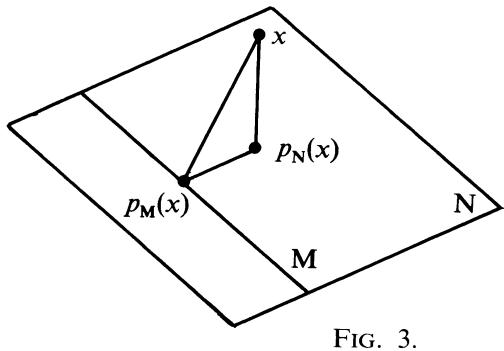
\includegraphics[keepaspectratio]{images/part002_dc4b20c6.jpg}}

\subsection{希尔伯特空间的对偶}

定理 3. --- 设 E 为希尔伯特空间。对每个 \(x \in E\) ，设 \(x^{*}\) 为 E 上的连续线性型 \(y \mapsto \langle x | y \rangle\) ；映射 \(x \mapsto x^{*}\) 是从 E 到其对偶上的一个双射的、半线性的映射（关于自同构 \(\xi \mapsto \overline{\xi}\) ），即从 E 到 \(E'\) 上，并且是从赋范空间 E 到赋范空间 \(E'\) 上的一个等距。

映射 \(x \mapsto x^*\) 由 (2)（V, p.~1）是半线性的，且由 Cauchy-Schwarz 不等式，我们有 \(\| x^* \| = \sup_{\| y \| \leqslant 1} |\langle x | y \rangle| = \| x \|\) ，故 \(x \mapsto x^*\) 是从 E 到 E' 中的一个等距，特别地是单射。为完成证明，需要证明对 E' 中所有 \(x' \neq 0\) ，存在 \(x \in E\) 使 \(x' = x^*\) 。而超平面 \(H = Ker x'\) 在 E 中是闭的；它的正交是一条直线 D。设 \(b\) 为 D 的一个非零元素；线性型 \(b^*\) 的核等于 H，因此存在标量 \(\lambda \neq 0\) 使 \(x' = \lambda . b^* = (\overline{\lambda}. b)^*\) 。证毕。

映射 \(x \mapsto x^{*}\) （从 E 到其对偶 \(E'\) 上的）称为典范映射。从 \(E'\) 到 E 上的逆映射也称为典范的，记作 \(x' \mapsto x'^{*}\) 。我们有

\[
\langle x | y \rangle = \langle y, x ^ {*} \rangle , \quad \langle x, x ^ {\prime} \rangle = \langle x ^ {\prime *} | x \rangle\tag{17}
\]

对 E 中的 \(x, y\) 与 E' 中的 \(x'\) 。还有 \((x^{*})^{*} = x\) 对 \(x \in \mathbf{E}\) 成立。

当 K 是 R 时，映射 \(x \mapsto x^{*}\) 是线性的。我们将用这个映射把 E 的内积转移到 \(E'\) 上。当 \(K = C\) 时，可以把映射 \(x \mapsto x^{*}\) 看作从向量空间 \(\overline{E}\) （E 的共轭）到 \(E'\) 上的同构（V, p.~6）。我们将用这个映射把 \(\overline{E}\) 的内积转移到 \(E'\) 上。

在所考虑的两种情形中，\(E'\) 是希尔伯特空间，且我们有公式

\[
\langle x ^ {*} | y ^ {*} \rangle = \overline {{\langle x | y \rangle}}, \quad \langle x ^ {\prime} | x ^ {\prime} \rangle = \| x ^ {\prime} \| ^ {2}
\]

对 \(x, y\) （\(\mathbf{E}\) 中的）与 \(x'\) （\(\mathbf{E}'\) 中的）。

说向量 \(x \in E\) 与向量 \(y \in E\) 正交，等价于说线性型 \(x^{*} \in E'\) 在 II, p.~41 所定义的意义下与 y 正交（这证明在两种情形下都可用«正交»一词）。若 M 是 E 的闭向量子空间，则与 M 正交的子空间 \(M^{\circ}\) （\(E'\) 中的，II, p.~44）是 E 中 M 的正交（定义于 V, p.~13）在 \(x \mapsto x^{*}\) 下的像（这证明在两种情形下都可用记号 \(M^{\circ}\)）。

推论 1. --- 为使希尔伯特空间 E 的点族 \((x_{i})_{i\in I}\) 是完全的，必要且充分的是：关系式 \(\langle x_{i}|y\rangle = 0\) （对 \(y \in E\) 且对所有指标 \(i \in I\) ）蕴含 y = 0。

事实上，这就是说 0 是 \(\mathbf{E}'\) 中与所有 \(x_{i}\) 正交的唯一的向量（II, p.~43 与 IV, p.~1）。

推论 2. --- 设 E 与 F 为两个希尔伯特空间。对 \(u \in \mathcal{L}(\mathrm{E};\mathrm{F})\) 、\(x \in \mathrm{E}\) 与 \(y \in \mathrm{F}\) ，令

\[
\Phi_ {u} (y, x) = \langle y | u (x) \rangle .\tag{18}
\]

映射 \(u \mapsto \Phi_u\) 是从 Banach 空间 \(\mathcal{L}(\mathrm{E};\mathrm{F})\) 到所有连续半双线性型 \(^1\) （\(\mathrm{F} \times \mathrm{E}\) 上的）组成的空间（赋以范数

\[
\| f\| = \sup_{\substack{x\in \mathbf{E},  y\in \mathbf{F}\\ \| x\| \leqslant 1, \| y\| \leqslant 1}}\left|f(y,x)\right|.\tag{19}
\]

显然 \(\Phi_u\) 对所有 \(u \in \mathcal{L}(\mathrm{E};\mathrm{F})\) 是半双线性的且连续的。反之，设 \(f\) 为 \(\mathrm{F} \times \mathrm{E}\) 上的连续半双线性型。对每个 \(x \in \mathrm{E}\) ，映射 \(y \mapsto \overline{f(y,x)}\) 是希尔伯特空间 \(\mathrm{F}\) 上的连续线性型。由定理 3，对每个 \(x \in \mathrm{E}\) ，存在唯一的元素 \(u(x)\) （在 \(\mathrm{F}\) 中）使 \(\overline{f(y,x)} = \langle u(x)|y\rangle\) 对所有 \(y \in \mathrm{F}\) 成立。映射 \(u: x \mapsto u(x)\) （从 \(\mathrm{E}\) 到 \(\mathrm{F}\) 中）是线性的，且我们有

\[
\begin{array}{l} \| f \| = \sup _ {\| x \| \leqslant 1} \sup _ {\| y \| \leqslant 1} | f (y, x) | = \sup _ {\| x \| \leqslant 1} \sup _ {\| y \| \leqslant 1} | \langle y | u (x) \rangle | \\ = \sup _ {\| x \| \leqslant 1} \| u (x) \|; \end{array}
\]

于是 \(u\) 属于 \(\mathcal{L}(\mathrm{E};\mathrm{F})\) ，\(f = \Phi_u\) 且 \(\| u\| = \| f\|\) 。这就证明了推论 2。

\(^{1}\) 回顾（A, IX, § 1, No.~5），F × E 上的（左）半双线性型 f 是从 F × E 到 K 中的映射，且满足 V, p.~1 的关系式 (1) 与 (2)。

从 E 到其双对偶 \(E''\) 的典范映射（IV, p.~14）把 E 映到 \(E''\) 上，换句话说（IV, p.~16），E 是自反 Banach 空间。事实上，若 E 是实（相应地，复）希尔伯特空间，则典范映射 \(\phi\) （从 \(E'\) 到 E 上的）是从赋范空间 \(E'\) 到 E（相应地，到 E 的共轭空间 \(\overline{E}\) ）上的一个同构；对 E（相应地，\(\overline{E}\) ）应用定理 3，我们看到赋范空间 \(E'\) 上的每个连续线性型都具有形式 \(x' \mapsto \langle \phi(x') | x \rangle = \langle x, x' \rangle\) ，其中 \(x \in E\) ，由此得出我们的断言。

作为推论（IV, p.~17, 命题 6）：

定理 4. --- 在希尔伯特空间 E 中，单位球是弱紧的。

命题 10. --- 若在希尔伯特空间 E 中，滤子 F 弱收敛于 \(x_{0}\) ，且又有 \(\lim_{\mathfrak{F}} \|x\| = \|x_{0}\|\) ，则 F 对 E 的初始拓扑收敛于 \(x_{0}\) 。事实上，\(\|x - x_{0}\|^{2} = \|x\|^{2} - 2R \langle x|x_{0} \rangle + \|x_{0}\|^{2}\) 。由于按假设 \(\langle x|x_{0}\rangle\) 关于 F 趋于 \(\|x_{0}\|^{2}\) ，且 \(\|x\|\) 关于 F 趋于 \(\|x_{0}\|\) ，故 \(\|x - x_{0}\|\) 关于 F 趋于 0，由此得命题。

注. --- 若 E 是 Hausdorff 准希尔伯特空间，\(\hat{E}\) 是 E 的希尔伯特空间完备化，我们知道（III, p.~16）E 的对偶 \(E'\) 可与 \(\hat{E}\) 的对偶等同；于是由定理 3（V, p.~15），E 上的每个连续线性型都可以唯一地写成 \(x \mapsto \langle a|x\rangle\) ，其中 \(a \in \hat{E}\) 。

\section{希尔伯特空间中的正交族}
% semantic-fragments: legacy-input-seam
\relax{}
\subsection{希尔伯特空间的外希尔伯特和}

命题 1. --- 设 \((\mathrm{E}_i)_{i\in \mathbf{I}}\) 为一族希尔伯特空间，\(\mathbf{P}\) 为乘积向量空间 \(\prod_{i\in \mathbf{I}}\mathrm{E}_i\)，\(\mathbf{E}\) 为 \(\mathbf{P}\) 中由所有家庭 \(\mathbf{x} = (x_i)_{i\in \mathbf{I}}\)（\(\sum_{i\in \mathbf{I}}\| x_i\|^2\) 为有限）组成的子集。

\begin{enumerate}
\def\labelenumi{\alph{enumi})}
\item
  E 是 \(\mathbf{P}\) 的向量子空间。
\item
  对 E 中的每个 \(\mathbf{x} = (x_i)_{i\in \mathbf{I}}\) 与 \(\mathbf{y} = (y_i)_{i\in \mathbf{I}}\)，族 \((\langle x_i|y_i\rangle)_{i\in \mathbf{I}}\) 可和。若令 \(\langle \mathbf{x}|\mathbf{y}\rangle = \sum_{i\in \mathbf{I}}\langle x_i|y_i\rangle\)，就在 E 上定义了一个正的非退化埃尔米特型。
\item
  对于如此定义的内积，\(\mathbf{E}\) 是希尔伯特空间；\(\mathbf{S}\) 是诸 \(\mathbf{E}_i\) 的直和，它在 \(\mathbf{E}\) 中稠密。
\end{enumerate}

对 E 中的 \(\mathbf{x} = (x_{i})_{i\in \mathbf{I}}\) 与 \(\mathbf{y} = (y_i)_{i\in \mathbf{I}}\)，我们有

\[
\left\| x _ {i} + y _ {i} \right\| ^ {2} \leqslant 2 \left(\left\| x _ {i} \right\| ^ {2} + \left\| y _ {i} \right\| ^ {2}\right),
\]

因而 \(\mathbf{x} + \mathbf{y} = (x_i + y_i)_{i\in I}\) 属于 E。这就证明了 \(a)\)。

由 Cauchy-Schwarz 不等式，我们有

\[
\left| \left\langle x _ {i} \mid y _ {i} \right\rangle \right| \leqslant \| x _ {i} \| \cdot \| y _ {i} \| \leqslant \frac {1}{2} \left(\left\| x _ {i} \right\| ^ {2} + \left\| y _ {i} \right\| ^ {2}\right)
\]

因而 \(\sum_{i\in \mathbf{I}}|\langle x_i|y_i\rangle | < +\infty\)。若 \(x\neq 0\)，我们有 \(\langle \mathbf{x}|\mathbf{x}\rangle = \sum_{i\in \mathbf{I}}\| x_i\|^2 >0\)，于是断言 \(b)\) 得证。

我们回顾，S 是 P 中由所有满足如下条件的家庭 \(\mathbf{x} = (x_{i})_{i \in \mathbf{I}}\) 组成的子空间：\(i \in I\) 中使 \(x_{i} \neq 0\) 的那些所成的集是有限的。由此立即推出 S 在 E 中稠密；于是只需证明 E 对拓扑 \(T_{1}\)（由范数 \(\|x\| = \langle x|x\rangle^{1/2}\) 得到）是完备的。设 \(T_{2}\) 为 \(\prod_{i \in I} E_{i}\) 上的乘积拓扑在 E 上诱导的拓扑。对每个 r \textgreater{} 0，设 \(B_{r}\) 为 \(x \in E\) 中所有满足 \(\|x\| \leqslant r\) 的元素组成的集。此关系式蕴含：对 I 的每个有限子集 J 都有 \(\sum_{i \in J} \|x_{i}\|^{2} \leqslant r^{2}\)，因而 \(B_{r}\) 是 \(\prod_{i \in I} E_{i}\) 的闭子集，从而也是完备的。于是 E 对 \(T_{1}\) 完备这一事实可由 GT, III, §3, No.~5, 命题 10 的推论 2 得出。

定义 1. --- 设 \((\mathrm{E}_{i})_{i\in\mathrm{I}}\) 为一族希尔伯特空间。命题 1 中定义的希尔伯特空间 E 称为族 \((\mathrm{E}_{i})_{i\in\mathrm{I}}\) 的外希尔伯特和，记作 \(\bigoplus_{i\in I} E_{i}\) 或 \(\bigoplus_{i\in I} E_{i}^{1}\)。

\(^{1}\) 应注意不要把这一记号与诸空间 \(E_{i}\) 的 « 代数 » 直和的记号（A, II, § 1, No.~6）相混淆。

设 \(f_{i}\) 为从 \(E_{i}\) 到 \(E\) 中的映射，它把 \(z \in E_{i}\) 变为满足如下条件的元素 \((x_{k}) \in E\)：\(x_{k} = 0\) 对所有 \(k \neq i\) 成立，且 \(x_{i} = z\)；显然 \(f_{i}\) 是从希尔伯特空间 \(E_{i}\) 到 \(E\) 的一个闭向量子空间上的同构。我们称 \(f_{i}\) 为从 \(E_{i}\) 到 \(E\) 中的典范映射，并且通常把 \(E_{i}\) 与它在此同构下的、\(E\) 中的像等同起来。在这一约定下，\(E_{i}\) 与 \(E_{k}\) 在 \(E\) 中正交（当 \(i \neq k\) 时），而 \(E\) 是由诸子空间 \(E_{i}\) 的并生成的闭向量子空间。

当 I 为有限时，E 是诸 \(E_{i}\) 的直和；由于从 E 到 \(E_{i}\) 上的典范投影算子对所有 \(i \in I\) 都连续，E 也是诸 \(E_{i}\) 的拓扑直和（GT, III, § 6, No.~2, 命题 2）。若 \(I = \left(1, n\right)\)，我们也用 \(E_{1} \oplus E_{2} \oplus \ldots \oplus E_{n}\) 来代替 \(\bigoplus_{i=1}^{n} E_{i}\)。

例. --- 设 E 为希尔伯特空间，I 为指标集。用 \(\ell_{\mathrm{E}}^{2}(\mathrm{I})\) 表示族 \((\mathrm{E}_{i})_{i\in\mathrm{I}}\)（其中 \(E_{i}=E\) 对所有 \(i\in I\) 成立）的外希尔伯特和。换言之，\(\ell_{\mathrm{E}}^{2}(\mathrm{I})\) 是由 E 中元素的所有家庭 \(\mathbf{x}=(x_{i})_{i\in\mathrm{I}}\)（满足 \(\sum_{i\in I}\|x_{i}\|^{2}<+\infty\)）组成的空间，赋以内积 \(\langle x|y\rangle=\sum_{i\in I}\langle x_{i}|y_{i}\rangle\)（以 I 为指标集的、E 中元素之平方可和家庭所成的空间）。我们令 \(\ell^{2}(\mathrm{I})=\ell_{\mathrm{K}}^{2}(\mathrm{I})\)。

\subsection{希尔伯特空间的正交子空间的希尔伯特和}

定义 2. --- 称希尔伯特空间 E 是其一族闭向量子空间 \((\mathbf{E}_{i})_{i\in I}\) 的希尔伯特和，如果：

\begin{enumerate}
\def\labelenumi{\arabic{enumi})}
\item
  对 I 中两个不同的指标 \(i\)、\(k\)，子空间 \(\mathrm{E}_i\) 与 \(\mathrm{E}_k\) 在 E 中正交；
\item
  由诸 \(\mathbf{E}_i\) 的并生成的闭向量子空间就是 E。
\end{enumerate}

定理 1. --- 设 E 为希尔伯特空间，它是一族闭向量子空间 \((\mathrm{E}_{i})_{i\in\mathbf{I}}\) 的希尔伯特和。存在唯一的、从 E 到 \(\bigoplus_{i\in I}E_{i}=F\)（族 \((\mathrm{E}_{i})\) 的外希尔伯特和）上的同构 f，使得对所有 \(i\in I\)，\(f\) 在 \(\mathbf{E}\) 上的限制就是典范映射 \(f_{i}\)（从 \(\mathbf{E}_i\) 到 \(\mathbf{F}\) 中）。

设 \(S \subset F\) 为诸 \(E_i\) 的 « 代数 » 直和，并设 \(g\) 为线性映射 \((x_i)_{i \in I} \mapsto \sum_{i \in I} x_i\)（从 \(S\) 到 \(E\) 中）。我们将证明 \(g\) 是从准希尔伯特空间 S 到（准希尔伯特）子空间 \(g(S)\)（E 的由诸 \(E_{i}\) 的并生成的子空间）上的同构：因为，对两个元素 \(\mathbf{x} = (x_{i})_{i \in \mathrm{I}}\)、\(\mathbf{y} = (y_{i})_{i \in \mathrm{I}}\)，我们有

\[
\langle g (\mathbf {x}) | g (\mathbf {y}) \rangle = \left\langle \sum_ {i \in \mathrm{I}} x _ {i} \right| \sum_ {i \in \mathrm{I}} y _ {i} \rangle = \sum_ {(i, k) \in \mathrm{I} \times \mathrm{I}} \left\langle x _ {i} \mid y _ {k} \right\rangle .
\]

但若 \(i \neq k\)，则由假设 \(\langle x_i | y_k \rangle = 0\)，因而

\[
\langle g (\mathbf {x}) | g (\mathbf {y}) \rangle = \sum_ {i \in \mathbf {I}} \langle x _ {i} | y _ {i} \rangle = \langle \mathbf {x} | \mathbf {y} \rangle ;
\]

这就证明了我们的断言。由于 S 在 F 中稠密且 \(g(S)\) 在 E 中稠密，同构 g 延拓为从 F 到 E 上的同构 \(\overline{g}\)（V, p.~8, 推论）。显然 \(\overline{g}\) 的逆同构 f 就是所求的映射；其唯一性由以下事实得出：E 中由诸 \(E_{i}\) 的并生成的闭子空间就是 E 自身。

当 E 是一族子空间 \((\mathrm{E}_{i})_{i\in I}\) 的希尔伯特和时，我们常借助同构 f 把 E 与诸 \(E_{i}\) 的外希尔伯特和 F 等同起来。~若集 I 为有限，则说 E 是族 \((\mathrm{E}_{i})_{i\in I}\) 的希尔伯特和，就意味着诸 \(E_{i}\) 两两正交，且向量空间 E 是子空间族 \((\mathrm{E}_{i})_{i\in I}\) 的直和。

推论 1. --- 设 E 为希尔伯特空间，它是一族闭向量子空间 \((\mathbf{E}_{i})_{i\in\mathbf{I}}\) 的希尔伯特和；对所有 \(i\in I\)，设 \(p_{E_{i}}\) 为从 E 到 \(E_{i}\) 上的正交投影算子（V, p.~13）。

\begin{enumerate}
\def\labelenumi{\alph{enumi})}
\tightlist
\item
  对所有 \(x \in \mathbb{E}\)，族 \((\| p_{\mathbf{E}_i}(x)\|^{2})_{i\in \mathbf{I}}\) 在 \(\mathbf{R}\) 中可和，族 \((p_{\mathbf{E}_i}(x))_{i\in \mathbf{I}}\) 在 \(\mathbb{E}\) 中可和，并且我们有
\end{enumerate}

\[
\left\| x \right\| ^ {2} = \sum_ {i \in \mathbf {I}} \left\| p _ {\mathrm{E} _ {i}} (x) \right\| ^ {2}, \quad x = \sum_ {i \in \mathbf {I}} p _ {\mathrm{E} _ {i}} (x).
\]

\begin{enumerate}
\def\labelenumi{\alph{enumi})}
\setcounter{enumi}{1}
\item
  反之，若 \((x_{i})_{i\in \mathbf{I}}\) 是 \(\mathbf{E}\) 中元素的一族，使得 \(x_{i}\in E_{i}\) 对所有 \(i\in \mathbf{I}\) 成立，且 \(\sum_{i\in \mathbf{I}}\| x_i\|^2 < + \infty\)，则此族可和，且其和 \(x\) 是 \(\mathbf{E}\) 中唯一的满足 \(p_{\mathrm{E}_i}(x) = x_i\)（对所有 \(i\in \mathbf{I}\)）的点。
\item
  对每一对点 \(x, y\)（属于 \(\mathbf{E}\)），我们有
\end{enumerate}

\[
\langle x | y \rangle = \sum_ {i \in \mathbf {I}} \left\langle p _ {\mathrm{E} _ {i}} (x) \mid p _ {\mathrm{E} _ {i}} (y) \right\rangle .
\]

这些性质对诸 \(\mathbf{E}_i\) 的外希尔伯特和而言事实上是显然的，并可经由同构转移到 \(\mathbf{E}\) 上。

推论 2. --- 设 E 为分离的准希尔伯特空间，\((\mathrm{E}_{i})_{i\in\mathrm{I}}\) 为 E 的一族完备向量子空间，使得对 I 中每一对不同的指标 i、k，子空间 \(E_{i}\) 与 \(E_{k}\) 正交。设 V 为 E 中由诸 \(E_{i}\) 的并生成的闭向量子空间。对每个 \(i\in I\)，设 \(p_{E_{i}}\) 为从 E 到 \(E_{i}\) 上的正交投影算子。设 \(x\in E\)。

\begin{enumerate}
\def\labelenumi{\arabic{enumi})}
\item
  我们有 \(\sum\left\|p_{E_{i}}(x)\right\|^{2}\leqslant\left\|x\right\|^{2}\)。
\item
  下列条件等价：a) \(x \in \mathbf{V}\)；b) \(\sum_{i \in I} \| p_{\mathrm{E}_i}(x) \|^2 = \| x \|^2\)；c) 族 \((p_{\mathrm{E}_i}(x))_{i \in I}\) 在 E 中可和，且 \(x = \sum_{i \in I} p_{\mathrm{E}_i}(x)\)。
\item
  假设 V 完备。则族 \((p_{\mathrm{E}_i}(x))_{i\in \mathbf{I}}\) 在 E 中可和，且
\end{enumerate}

\[
p _ {\mathbf {V}} (x) = \sum_ {i \in \mathbf {I}} p _ {\mathrm{E} _ {i}} (x), \quad \left\| p _ {\mathbf {V}} (x) \right\| ^ {2} = \sum_ {i \in \mathbf {I}} \left\| p _ {\mathrm{E} _ {i}} (x) \right\| ^ {2},
\]

其中 \(p_{V}\) 表示从 E 到 V 上的正交投影算子。

设 \(\hat{\mathbf{E}}\) 为 \(\mathbf{E}\) 的希尔伯特空间完备化；我们把 \(\mathbf{E}\) 与 \(\hat{\mathbf{E}}\) 的一个稠密子空间等同起来；诸 \(\mathbf{E}_i\) 因完备而是 \(\hat{\mathbf{E}}\) 的闭子空间。闭包 \(\overline{\mathbf{V}}\)（\(\mathbf{V}\) 在 \(\hat{\mathbf{E}}\) 中的闭包）是 \(\hat{\mathbf{E}}\) 中由诸 \(\mathbf{E}_i\) 的并生成的闭向量子空间，且 \(\mathbf{V} = \overline{\mathbf{V}} \cap \mathbf{E}\)。空间 \(\hat{\mathbf{E}}\) 是诸 \(\mathbf{E}_i\) 与子空间 \(\mathbf{W}\)（即 \(\overline{\mathbf{V}}\) 在 \(\hat{\mathbf{E}}\) 中的正交补）的希尔伯特和；令 \(x_0 = p_{\mathrm{W}}(x)\) 与 \(x_i = p_{\mathrm{E}_i}(x)\)（对所有 \(i \in \mathbf{I}\)）。由推论 1，我们有 \(\| x\|^2 = \| x_0\|^2 + \sum_{i \in \mathbf{I}} \| x_i\|^2\)，且 \(x = x_0 + \sum_{i \in \mathbf{I}} x_i\)（在 \(\hat{\mathbf{E}}\) 中）。由此即得断言 1)，以及 2) 的条件 \(b)\) 与 \(c)\) 等价于条件 \(x_0 = 0\)、从而等价于条件 \(x \in \mathbf{V}\) 这一事实。最后，若 \(\mathbf{V}\) 完备，并令 \(x' = p_{\mathrm{V}}(x)\)，我们有 \(x' - x_i = (x - x_i) - (x - p_{\mathrm{V}}(x))\)，因而 \(x' - x_i\) 与 \(\mathbf{E}_i\) 正交，于是 \(x_i = p_{\mathrm{E}_i}(x')\) 对所有 \(i \in \mathbf{I}\) 成立；此时只需对向量 \(x'\) 应用性质 2) 即可。

注. --- 设 E 为分离的准希尔伯特空间，\((\mathrm{V}_{i})_{i\in\mathrm{I}}\) 为 E 的一族向量子空间，使得对每一对不同的指标 i、k，子空间 \(V_{i}\) 与 \(V_{k}\) 正交。于是，对每个 \(k\in I\)，\(V_{k}\) 与闭向量子空间 \(W_{k}\)（由诸 \(V_{i}\)（\(i\neq k\)）的并生成）的交化为 0；因为，若 x 既属于 \(V_{k}\) 又属于 \(W_{k}\)，则它与所有 \(V_{i}\)（\(i\neq k\)）正交，从而与 \(W_{k}\) 正交。特别地，x 与自身正交，故为零。

命题 2. --- 设 E 为希尔伯特空间，\((\mathrm{V}_{\lambda})_{\lambda\in\mathrm{L}}\) 为 E 的一族闭向量子空间；对每个 \(\lambda\in L\)，设 \((\mathrm{W}_{\lambda\mu})_{\mu\in\mathrm{M}_{\lambda}}\) 为 \(V_{\lambda}\) 的一族闭向量子空间，使得 \(V_{\lambda}\) 是由此族之并生成的闭向量子空间。为使 E 是族 \((\mathrm{W}_{\lambda\mu})_{\lambda\in\mathrm{L},\mu\in\mathrm{M}_{\lambda}}\) 的希尔伯特和，必要且充分的是：E 是族 \((\mathrm{V}_{\lambda})_{\lambda\in\mathrm{L}}\) 的希尔伯特和，且对每个 \(\lambda\in L\)，\(V_{\lambda}\) 是族 \((\mathrm{W}_{\lambda\mu})_{\mu\in\mathrm{M}_{\lambda}}\) 的希尔伯特和（« 希尔伯特和的结合性 »）。为证条件必要，只需看出 \(V_{\alpha}\) 与 \(V_{\beta}\) 正交（若 \(\alpha\neq\beta\)）。但是，\(W_{\alpha\mu}\)（\(\mu\in M_{\alpha}\)）的每个元素与所有 \(W_{\beta\nu}\)（\(\nu\in M_{\beta}\)）正交，从而与它们所生成的闭向量子空间 \(V_{\beta}\) 正交；同样的论证进而表明 \(V_{\beta}\) 的每个元素与 \(V_{\alpha}\) 正交，因为它与所有 \(W_{\alpha\mu}\)（\(\mu\in M_{\alpha}\)）正交。

为证条件充分，只需验证：若条件满足，则 \(\mathrm{E}\) 等于闭向量子空间 \(\mathrm{F}\)（由诸 \(\mathbf{W}_{\lambda \mu}\)（\(\lambda \in \mathbf{L}\)，\(\mu\in M_{\lambda}\)）的并生成）；而对每个 \(\lambda\in L\)，F 包含由诸 \(W_{\lambda\mu}\)（其中 \(\mu\in M_{\lambda}\)）的并生成的闭向量子空间，也就是说 F 包含 \(V_{\lambda}\)；于是 F 是由诸 \(V_{\lambda}\) 的并生成的闭向量子空间，而由假设它就是 E。

\subsection{标准正交族}

定义 3. --- 在准希尔伯特空间中，称向量族 \((e_{i})_{i\in\mathbf{I}}\) 为正交的，如果 \(e_{i}\) 与 \(e_{k}\)（对所有 \(i\neq k\)）正交；称其为标准正交的，如果此外 \(\|e_{i}\|=1\) 对所有 \(i\in I\) 成立。

E 的子集 S，若由 S 到其自身的恒等映射所定义的族是标准正交的，则称之为标准正交集。若 \((e_{i})_{i\in I}\) 是标准正交族，则映射 \(i\mapsto e_{i}\) 是单射；于是我们可以不加区分地谈论标准正交族或标准正交集。

若 \((e_i)_{i\in I}\) 是标准正交族，则完备的一维向量子空间 \(\mathbf{D}_i = \mathbf{K}e_i\) 两两正交。对每个 \(x\in E\)，\(x\) 在 \(\mathbf{D}_i\) 上的正交投影是 \(\lambda_i e_i\)，其中 \(\langle e_i|x - \lambda_i e_i\rangle = 0\)，由此得 \(\langle e_i|x\rangle = \lambda_i\langle e_i|e_i\rangle = \lambda_i\)。将 No.~2 的结果应用于诸子空间 \(\mathbf{D}_i\)，便得到下列命题：

命题 3. --- 在分离的准希尔伯特空间 E 中，每个标准正交族都是拓扑无关的。

我们注意到，这一性质可由拓扑无关族的刻画（IV, p.~1 与 II, p.~43, 推论 2）立即得出，因为按 K 等于 R 或 C，E 的对偶分别与 E 的完备化或 E 的共轭空间等同（V, p.~17, 注）。

命题 4. --- 设 E 为分离的准希尔伯特空间，\((e_{i})_{i\in I}\) 为 E 中的标准正交族，V 为 E 中由诸 \(e_{i}\) 生成的闭向量子空间。

\begin{enumerate}
\def\labelenumi{\arabic{enumi})}
\tightlist
\item
  对每个 \(x \in E\)，我们有
\end{enumerate}

\[
\sum_ {i \in \mathbf {I}} \left| \langle e _ {i} | x \rangle \right| ^ {2} \leqslant \| x \| ^ {2}\tag{1}
\]

（Bessel 不等式）；这里，所有 \(i \in \mathbf{I}\) 中使 \(\langle e_i|x\rangle \neq 0\) 者所成的集是可数的。此外，下列条件等价：a) \(x \in \mathbf{V}\)；b) \(\|x\|^2 = \sum_{i \in \mathbf{I}} |\langle e_i|x\rangle|^2\)；c) 族 \(\langle e_i|x\rangle\) . \(e_i\) 在 E 中可和，且 \(x = \sum_{i \in \mathbf{I}} \langle e_i|x\rangle\) . \(e_i\)。

\begin{enumerate}
\def\labelenumi{\arabic{enumi})}
\setcounter{enumi}{1}
\item
  若 \(\mathbf{V}\) 完备，则由所有 \(\langle e_i|x\rangle\) . \(e_i\) 组成的族在 \(\mathbf{E}\) 中（对所有 \(x\in\mathbf{E}\)）可和，且 \(\sum_{i\in\mathbf{I}}\langle e_i|x\rangle\) . \(e_i=p_{\mathbf{V}}(x)\)，\(\sum_{i\in\mathbf{I}}|\langle e_i|x\rangle|^2=\|p_{\mathbf{V}}(x)\|^2\)。
\item
  假设 V 完备。对每个标量族 \((\lambda_{i})_{i\in\mathbf{I}}\)（满足 \(\sum_{i\in I}|\lambda_{i}|^{2}<+\infty\)），存在唯一的点 \(x\in V\)，使得 \(\langle e_{i}|x\rangle=\lambda_{i}\) 对所有 \(i\in I\) 成立。若 \((\mu_{i})_{i\in I}\) 是第二个满足 \(\sum_{i\in I}\left|\mu_{i}\right|^{2}<+\infty\) 的标量族，且 \(y\in V\) 满足 \(\langle e_{i}|y\rangle=\mu_{i}\)（对所有 \(i\in I\)），则 \(\langle x|y\rangle=\sum_{i\in I}\overline{\lambda}_{i}\mu_{i}\)。
\end{enumerate}

命题 5. --- 设 \((e_i)_{i \in I}\) 为分离的准希尔伯特空间 E 中的标准正交族。下列性质等价：

\begin{enumerate}
\def\labelenumi{\alph{enumi})}
\item
  族 \((e_i)\) 是完全的；
\item
  对每个 \(x \in E\)，族 \(\langle e_{i}|x\rangle\) . \(e_{i}\) 在 E 中可和，且 \(x = \sum_{i \in I} \langle e_{i}|x\rangle\) . \(e_{i}\)；
\item
  对每个 \(x \in E\)，
\end{enumerate}

\[
\left\| x \right\| ^ {2} = \sum_ {i \in \mathbf {I}} \left| \langle e _ {i} | x \rangle \right| ^ {2}\tag{2}
\]

（Parseval 等式）。

当 E 是希尔伯特空间时，这些条件也等价于：

\begin{enumerate}
\def\labelenumi{\alph{enumi})}
\setcounter{enumi}{3}
\tightlist
\item
  关系式 \(\langle e_i|x\rangle = 0\)（对所有 \(i\in \mathrm{I}\)）蕴含 \(x = 0\)。
\end{enumerate}

条件 a)、b)、c) 的等价性由命题 4 立即得出。当 E 是希尔伯特空间时，条件 a) 与 d) 的等价性由 V, p.~16 的推论 1 得出。

定义 4. --- 分离的准希尔伯特空间 E 中的标准正交且完全的族称为 E 的标准正交基。

分离的准希尔伯特空间 E 的标准正交基也是 E 的完备化的标准正交基。

设 \((e_{i})_{i\in I}\) 为 E 的标准正交基；对每个 \(x\in E\)，数 \(\langle e_{i}|x\rangle\) 滥用术语称为 x 关于基 \((e_{i})\) 的坐标。对 E 中每个 x 与 y，我们有

\[
\langle x | y \rangle = \sum_ {i \in \mathbf {I}} \overline {{\langle e _ {i} | x \rangle}} \langle e _ {i} | y \rangle .\tag{3}
\]

E 的标准正交基一般并不是 A, II, p.~25 中所定义的意义下 E 在域 K 上的基；为避免任何混淆，我们把上述引文意义下准希尔伯特空间 E 的基称为 E 在 K 上的代数基。

设 E 与 F 为两个分离的准希尔伯特空间，u 为从 E 到 F 中的连续线性映射。设 \((e_{i})_{i\in I}\)（相应地，\((f_{j})_{j\in J}\)）为 E（相应地，F）的标准正交基。令

\[
u _ {j i} = \langle f _ {j} | u (e _ {i}) \rangle
\]

其中 \(i \in \mathbf{I}\)，\(j \in \mathbf{J}\)。族 \((u_{ji})_{(i,j) \in \mathbf{I} \times \mathbf{J}}\) 称为 \(u\) 关于标准正交基 \((e_i)\) 与 \((f_j)\) 的矩阵。设 \(x \in \mathbf{E}\) 且 \(y = u(x)\)；若分别用 \(\xi_i = \langle e_i | x \rangle\) 与 \(\eta_j = \langle f_j | y \rangle\) 表示 \(x\) 与 \(y\) 的坐标，则 \(\eta_j = \sum_{i \in \mathbf{I}} u_{ji} \xi_i\) 对所有 \(j \in \mathbf{J}\) 成立。当 \((e_i)\) 是 \(E\) 的代数基且 \((f_j)\) 是 \(F\) 的代数基时，我们的定义与 A, II, § 10, No.~4 中的定义一致。

例. --- 设 E 为 R 上复值连续函数的空间，这些函数满足 \(f(x + n) = f(x)\)（\(x \in R\)，\(n \in Z\)）。我们赋予 E 由下式定义的内积

\[
\langle f | g \rangle = \int_ {0} ^ {1} \overline {{{{f (t)}}}} g (t) d t.
\]

于是 E 是分离的准希尔伯特空间，但不完备。对每个整数 \(n \in Z\)，令 \(e_{n}(x) = \mathbf{e}(nx)\)。立即可以看出族 \((e_{n})_{n \in \mathbf{Z}}\) 在 E 中标准正交。此外，E 上的一致收敛拓扑细于由范数 \(\|f\|_{2} = \langle f | f \rangle^{1/2}\) 得到的拓扑。族 \((e_{n})_{n \in \mathbf{Z}}\) 在 E 中对一致收敛是完全的（GT, X, § 4, No.~4），从而在准希尔伯特空间 E 中更是完全的。因此 \((e_{n})_{n \in \mathbf{Z}}\) 是 E 的标准正交基。

\subsection{标准正交化}

定理 2. --- 对希尔伯特空间 E 中的每个标准正交集 L，存在 E 的包含 L 的标准正交基 B。

事实上，设 D 为 E 的所有标准正交子集按包含关系线性排序所成的族；立即可以看出此族具有有限特征（S, III, § 4, No.~5）。于是由 S, III, § 4, No.~5 的定理 1，D 中存在包含 L 的极大族 B。剩下要证 B 是完全集。若不然，将存在一个与 B 的所有向量都正交的向量 \(y \neq 0\)（V, p.~22, 命题 5），用适当的标量乘 y，可设 \(\|y\| = 1\)；那么 \(B \cup \{y\}\) 将是异于 B 且包含 B 的标准正交集；这与 B 的定义矛盾；定理得证。

推论 1. --- 在每个希尔伯特空间中都存在标准正交基。

只需对 L = ∅ 的情形应用定理 2。

推论 2. --- 每个希尔伯特空间都同构于某个空间 \(\ell^2 (\mathbf{I})\)。

更确切地说，设 \((e_{i})_{i\in I}\) 为希尔伯特空间 E 的标准正交基。由命题 4（V, p.~21）与命题 5（V, p.~22），由下式定义的映射 \(\phi\)

\[
\phi (x) = \big (\langle e _ {i} | x \rangle \big) _ {i \in \mathrm{I}}\tag{4}
\]

是从 E 到 \(\ell^2 (\mathrm{I})\) 上的希尔伯特空间同构。逆同构 \(\psi\) 由下式定义

\[
\psi ((\lambda_ {i}) _ {i \in \mathbf {I}}) = \sum_ {i \in \mathbf {I}} \lambda_ {i} e _ {i}.\tag{5}
\]

命题 6. --- 设 E 为分离的准希尔伯特空间，\((a_{n})_{n\in\mathbb{I}}\)（I 是 N 的以 1 为起点的区间）为 E 中向量的一个可数的（有限或无限）无关族。则存在唯一的 E 中的标准正交族 \((e_{n})_{n\in\mathbb{I}}\)，具有下列性质：

\begin{enumerate}
\def\labelenumi{\arabic{enumi})}
\item
  对每个整数 \(p \in \mathbf{I}\)，\(\mathbf{E}\) 的由 \(e_1, e_2, \ldots, e_p\) 生成的向量子空间与 \(\mathbf{E}\) 的由 \(a_1, a_2, \ldots, a_p\) 生成的向量子空间相同；
\item
  对每个整数 \(p \in \mathbf{I}\)，数 \(\langle a_p | e_p \rangle\) 是实数且 \(> 0\)。
\end{enumerate}

事实上，设 \(V_{n}\) 为由 \(a_{1}, a_{2}, ..., a_{n}\) 生成的（n 维）子空间。若 \(n + 1 \in I\) 且 \(b_{n+1} = a_{n+1} - p_{\mathrm{V}_{n}}(a_{n+1})\)（其中 \(p_{V_{n}}\) 是到完备子空间 \(V_{n}\) 上的正交投影算子），则直线 \(Kb_{n+1}\) 是 \(V_{n}\) 在 \(V_{n+1}\) 中的正交（补）。若诸 \(e_{n}\) 满足命题的条件 1)，则必须有 \(e_{n+1} = \lambda b_{n+1}\)；条件 \(\|e_{n+1}\| = 1\) 于是蕴含 \(|\lambda|^2 \|b_{n+1}\|^2 = 1\)，而条件 \(\langle a_{n+1}|e_{n+1} \rangle > 0\) 蕴含 \(\lambda \langle a_{n+1}|b_{n+1} \rangle > 0\)；这就完全确定了 \(\lambda\)，于是我们证明了可以用归纳法确定唯一的标准正交族 \((e_n)_{n\in I}\)，使之满足命题的条件 1) 与 2)。

称序列 \((e_{n})_{n\in\mathbb{I}}\) 是由无关族 \((a_{n})_{n\in\mathbb{I}}\) 经标准正交化得到的。显然，由族 \((e_{n})\) 生成的向量子空间与由族 \((a_{n})\) 生成的向量子空间相同。特别地，若 \((a_{n})\) 是完全序列，则 \((e_{n})\) 也是，从而它是 E 的标准正交基；由此得到：

推论. --- 在每个满足第一可数公理的分离准希尔伯特空间 E 中，都存在可数的标准正交基。

若 E 满足第一可数公理，则 E 中存在完全序列，而且总能从此序列中抽取一个无关的完全族（A, II, § 7, No.~1, 定理 2）。

可以举出没有任何标准正交基的分离准希尔伯特空间的例子（V, p.~70, 练习 2）。

例. --- 设 I 为 R 的区间 \((-1,1)\)，E 为 I 上实值连续函数的向量空间。用 x 表示从 I 到 R 中的典范单射，把它看作 E 的一个元素。由 Stone-Weierstrass 定理，序列 \((x^{n})_{n\in\mathbf{N}}\) 在 E 中对一致收敛拓扑是完全的（GT, X, § 4, No.~2）。

把 E 看作实的分离准希尔伯特空间，其内积由下式给出

\[
\langle f | g \rangle = \int_ {- 1} ^ {1} f (t) g (t) d t.
\]

于是序列 \((x^{n})_{n\in \mathbb{N}}\) 在准希尔伯特空间 E 中是完全的。设 \((\Pi_n)_{n\in \mathbb{N}}\) 为由序列 \((x^n)_{n\in \mathbb{N}}\) 经标准正交化得到的序列。可以证明 \(\Pi_n = (n + \frac{1}{2})^{1 / 2}\mathbf{P}_n\)，其中 Legendre 多项式 \(\mathbf{P}_n\) 由下式定义

\[
\mathrm{P} _ {n} (x) = \frac {1}{2 ^ {n} n !} \left(\frac {d}{d x}\right) ^ {n} (x ^ {2} - 1) ^ {n}.
\]

命题 7. --- 在希尔伯特空间 E 中，两个标准正交基是等势的。

设 B 与 C 为 E 的两个标准正交基。当两集 B、C 之一为有限时，情形是平凡的，因为有限的标准正交基是空间的代数基。因此设 B 与 C 都是无限的。对每个 \(x \in B\)，设 \(C_{x}\) 为由 \(y \in C\) 中所有使 \(\langle x | y \rangle \neq 0\) 者组成的子集。集 \(C_{x}\) 是可数的（V, p.~21, 命题 4）。对每个 \(y \in C\)，存在 \(x \in B\) 使 \(y \in C_{x}\)，因为 B 是标准正交基且 \(y \neq 0\)；换言之，C 是当 x 取遍 B 时诸可数集 \(C_{x}\) 的并。于是 C 的基数小于 N × B 的基数，从而小于 B 的基数（S, III, §6, No.~3, 推论 4）；类似地，B 的基数小于 C 的基数；证明完毕。

希尔伯特空间 E 的任一标准正交基的基数称为 E 的希尔伯特维数。

推论 1. --- 给定希尔伯特空间 E 中的两个标准正交基，存在 E 的自同构把第一个基变为第二个基。

推论 2. --- 为使希尔伯特空间 \(\ell^2 (\mathbf{I})\) 与 \(\ell^2 (\mathbf{J})\) 同构，必要且充分的是 I 与 J 等势。

\section{希尔伯特空间的张量积}

\subsection{准希尔伯特空间的张量积}

设 \(E_{1}\) 与 \(E_{2}\) 为两个准希尔伯特空间，\(F = E_{1} \otimes E_{2}\) 为向量空间 \(E_{1}\) 与 \(E_{2}\) 的张量积。设 \(x_{1} \in E_{1}\) 且 \(x_{2} \in E_{2}\)；由于映射 \((y_{1}, y_{2}) \mapsto \langle x_{1}|y_{1} \rangle \langle x_{2}|y_{2} \rangle\)（从 \(E_{1} \times E_{2}\) 到 K 中）是双线性的，故存在线性型 \(\phi_{x_{1},x_{2}}\)（在 \(E_{1} \otimes E_{2}\) 上），使得

\[
\phi_ {x _ {1}, x _ {2}} (y _ {1} \otimes y _ {2}) = \langle x _ {1} | y _ {1} \rangle \langle x _ {2} | y _ {2} \rangle\tag{1}
\]

其中 \(y_{1} \in \mathrm{E}_{1}\)，\(y_{2} \in \mathrm{E}_{2}\)。设 \(z \in \mathrm{F}\)。映射 \((x_{1}, x_{2}) \mapsto \overline{\phi_{x_{1},x_{2}}(z)}\)（从 \(\mathrm{E}_1 \times \mathrm{E}_2\) 到 \(\mathbf{K}\) 中）是双线性的；把 \(z\) 写成形式 \(z = \sum_{i=1}^{n} y_{i,1} \otimes y_{i,2}\)（其中 \(y_{i,1} \in \mathrm{E}_1\)、\(y_{i,2} \in \mathrm{E}_2\)，\(1 \leqslant i \leqslant n\)）即可看出这一点。于是存在线性型 \(\psi_z\)（在 \(\mathrm{F} = \mathrm{E}_1 \otimes \mathrm{E}_2\) 上），使得

\[
\psi_ {z} (x _ {1} \otimes x _ {2}) = \overline {{\phi_ {x _ {1} , x _ {2}} (z)}} \quad (x _ {1} \in \mathrm{E} _ {1}, x _ {2} \in \mathrm{E} _ {2}).\tag{2}
\]

我们令 \(\Phi(z, t) = \psi_z(t)\)（对 F 中的 \(z, t\)）。立即可以看出 \(\Phi\) 是 \(\mathbf{E}_1 \otimes \mathbf{E}_2\) 上的一个半双线性型，它由下式刻画

\[
\Phi (x _ {1} \otimes x _ {2}, y _ {1} \otimes y _ {2}) = \langle x _ {1} | y _ {1} \rangle \langle x _ {2} | y _ {2} \rangle\tag{3}
\]

(cf.~A, IX, § 1, No.~11).

命题 1. --- 半双线性型 \(\Phi\)（在 \(\mathrm{E}_1 \otimes \mathrm{E}_2\) 上）是埃尔米特型且是正的，因而它给 \(\mathrm{E}_1 \otimes \mathrm{E}_2\) 赋予了准希尔伯特空间的结构。若 \(\mathrm{E}_1\) 与 \(\mathrm{E}_2\) 是分离的，则此空间是分离的。

公式 \(\Phi(z, t) = \overline{\Phi(t, z)}\) 当 \(z = x_1 \otimes x_2\) 且 \(t = y_1 \otimes y_2\) 时由 (3) 得出。一般情形由线性性得到，因而 \(\Phi\) 是埃尔米特型。

设 \(\mathbf{E}_1\) 与 \(\mathbf{E}_2\) 是分离的；我们将证明埃尔米特型 \(\Phi\) 是正的且非退化。设 \(z = \sum_{i=1}^{n} x_i \otimes y_i\) 为 \(\mathrm{F} = \mathrm{E}_1 \otimes \mathrm{E}_2\) 的非零元素。设 \((e_1, ..., e_n)\) 为 \(\mathbf{E}_1\) 中由 \(x_1, ..., x_n\) 生成的子空间的标准正交基（V, p.~23, 推论 1）。存在元素 \(f_1, ..., f_m\)（在 \(\mathbf{E}_2\) 中，不全为零），使得 \(z = \sum_{i=1}^{n} e_i \otimes f_i\)，因而

\[
\begin{array}{l} \Phi (z, z) = \sum_ {i, j = 1} ^ {m} \Phi (e _ {i} \otimes f _ {i}, e _ {j} \otimes f _ {j}) \\ = \sum_ {i, j} \langle e _ {i} | e _ {j} \rangle \langle f _ {i} | f _ {j} \rangle = \sum_ {i = 1} ^ {m} \| f _ {i} \| ^ {2} > 0. \end{array}
\]

对一般情形，我们现在来证明 \(\Phi\) 是正的。设 \(\tilde{E}_{i}\) 为与 \(E_{i}\) 相伴的分离准希尔伯特空间，\(\pi_{i}\) 为从 \(E_{i}\) 到 \(\tilde{E}_{i} (i = 1, 2)\) 上的典范映射。令 \(\pi = \pi_{1} \otimes \pi_{2}\)。设 \(\tilde{\Phi}\) 为 \(\tilde{E}_{1} \otimes \tilde{E}_{2}\) 上按与 \(\Phi\) 相同的方式构造的埃尔米特型。我们有

\[
\Phi (z, t) = \Phi (\pi (z), \pi (t)) \quad (z \in \mathrm{F}, t \in \mathrm{F}),
\]

而由于 \(\tilde{\Phi}\) 是正的，\(\Phi\) 也是正的。

证毕。

命题 1 中定义的准希尔伯特空间称为准希尔伯特空间 \(E_{1}\) 与 \(E_{2}\) 的张量积，记作 \(E_{1} \otimes E_{2}\)。此后我们将用 \(\langle z|t\rangle\) 表示 \(\Phi(z,t)\)，于是依定义

\[
\langle x _ {1} \otimes x _ {2} | y _ {1} \otimes y _ {2} \rangle = \langle x _ {1} | y _ {1} \rangle \langle x _ {2} | y _ {2} \rangle ;\tag{4}
\]

我们也用 \(\| z\| _2\) 或 \(\| z\|\) 来记 \(\langle z|z\rangle^{1 / 2}\)。由 (4) 得

\[
\left\| x _ {1} \otimes x _ {2} \right\| _ {2} = \left\| x _ {1} \right\|. \left\| x _ {2} \right\|,\tag{5}
\]

于是双线性映射 \((x_{1}, x_{2}) \mapsto x_{1} \otimes x_{2}\)（从 \(\mathrm{E}_1 \times \mathrm{E}_2\) 到 \(\mathrm{E}_1 \otimes \mathrm{E}_2\) 中）是连续的。

对 i = 1, 2，设 \(F_{i}\) 为 \(E_{i}\) 的向量子空间，赋以诱导的准希尔伯特结构。于是 \(F_{1} \otimes F_{2}\) 可与 \(E_{1} \otimes E_{2}\) 的一个向量子空间等同（A, II, § 7, No.~7）。公式 (4) 表明，\(F_{1} \otimes F_{2}\) 赋以由 \(E_{1} \otimes_{2} E_{2}\) 的结构诱导的准希尔伯特空间结构后，恰好就是 \(F_{1} \otimes_{2} F_{2}\)。此后我们将把 \(F_{1} \otimes_{2} F_{2}\) 与 \(E_{1} \otimes_{2} E_{2}\) 的准希尔伯特子空间等同起来。

命题 2. --- 对 \(i = 1, 2\)，设 \(\mathrm{E}_{i}\) 与 \(\mathrm{F}_{i}\) 为两个分离的准希尔伯特空间，并设 \(u_{i} \in \mathcal{L}(\mathrm{E}_{i}; \mathrm{F}_{i})\)。线性映射 \(u_{1} \otimes u_{2}\)（从 \(\mathrm{E}_{1} \otimes_{2} \mathrm{E}_{2}\) 到 \(\mathrm{F}_{1} \otimes_{2} \mathrm{F}_{2}\) 中）是连续的，并且我们有

\[
\left\| u _ {1} \otimes u _ {2} \right\| = \left\| u _ {1} \right\|. \left\| u _ {2} \right\|.
\]

考虑 \(\mathbf{E}_1\) 上由下式给出的正埃尔米特型

\[
f \left(x _ {1}, y _ {1}\right) = \| u _ {1} \| ^ {2} \left\langle x _ {1} \mid y _ {1} \right\rangle - \left\langle u _ {1} \left(x _ {1}\right) \mid u _ {1} \left(y _ {1}\right) \right\rangle .
\]

由命题 1（V, p.~25），存在正埃尔米特型 \(\Phi\)（在 \(E_1 \otimes E_2\) 上），使得

\[
\begin{array}{r l} \Phi (x _ {1} \otimes x _ {2}, y _ {1} \otimes y _ {2}) & = f (x _ {1}, y _ {1}) \langle x _ {2} | y _ {2} \rangle = \\ & = \| u _ {1} \| ^ {2} \langle x _ {1} \otimes x _ {2} | y _ {1} \otimes y _ {2} \rangle - \langle (u _ {1} \otimes 1) (x _ {1} \otimes x _ {2}) | (u _ {1} \otimes 1) (y _ {1} \otimes y _ {2}) \rangle \end{array}
\]

其中 \(x_{1}, y_{1}\) 属于 \(E_{1}\)，\(x_{2}, y_{2}\) 属于 \(E_{2}\)。由线性性得

\[
\Phi (z, t) = \| u _ {1} \| ^ {2} \langle z | t \rangle - \langle (u _ {1} \otimes 1) (z) | (u _ {1} \otimes 1) (t) \rangle
\]

其中 \(z, t\) 属于 \(\mathrm{E}_1 \otimes \mathrm{E}_2\)。由于 \(\Phi\) 是正的，得 \(\Phi(z, z) \geqslant 0\)，即 \(\| (u_1 \otimes 1).z \|_2\) \(\leqslant \| u_1\| \cdot \| z\| _2\)（对 \(z\in \mathrm{E}_1\otimes_2\mathrm{E}_2\)），亦即 \(\| u_1\otimes 1\| \leqslant \| u_1\|\)。同理可证不等式 \(\| 1\otimes u_2\| \leqslant \| u_2\|\)；又由于 \(u_{1}\otimes u_{2} = (u_{1}\otimes 1)\circ (1\otimes u_{2})\)，我们得到

\[
\left\| u _ {1} \otimes u _ {2} \right\| \leqslant \left\| u _ {1} \right\|. \left\| u _ {2} \right\|.
\]

另一方面，

\[
\begin{array}{l} \| u _ {1} \| \cdot \| u _ {2} \| = \sup _ {\| x _ {1} \| \leqslant 1, \| x _ {2} \| \leqslant 1} \| u _ {1} (x _ {1}) \| \cdot \| u _ {2} (x _ {2}) \| \\ = \sup _ {\| x _ {1} \| \leqslant 1, \| x _ {2} \| \leqslant 1} \| (u _ {1} \otimes u _ {2}) (x _ {1} \otimes x _ {2}) \| _ {2} \leqslant \| u _ {1} \otimes u _ {2} \|. \end{array}
\]

这样就完成了命题 2 的证明。

证毕。

设 \(E_1, \ldots, E_n\) 为准希尔伯特空间（\(n \geqslant 2\)）。我们用归纳法以下式定义张量积 \(E_1 \otimes_2 \ldots \otimes_2 E_n\)（也记作 \(\bigotimes_{i=1}^{n} E_i\)）

\[
\mathrm{E} _ {1} \otimes_ {2} \dots \otimes_ {2} \mathrm{E} _ {n} = (\mathrm{E} _ {1} \otimes_ {2} \dots \otimes_ {2} \mathrm{E} _ {n - 1}) \otimes_ {2} \mathrm{E} _ {n}.
\]

于是，由内积的定义，我们有

\[
\left\langle x _ {1} \otimes \dots \otimes x _ {n} \mid y _ {1} \otimes \dots \otimes y _ {n} \right\rangle = \prod_ {i = 1} ^ {n} \left\langle x _ {i} \mid y _ {i} \right\rangle ,\tag{6}
\]

特别地 \(^{1}\)

\[
\left\| x _ {1} \otimes \dots \otimes x _ {n} \right\| _ {2} = \left\| x _ {1} \right\| \dots \left\| x _ {n} \right\|,\tag{7}
\]

其中 \(x_{i},y_{i}\) 属于 \(\mathrm{E}_i\)（\(1\leqslant i\leqslant n\)）。若诸 \(\mathrm{E}_i\) 都是分离的，则 \(\mathrm{E}_1\otimes_2\dots \otimes_2\mathrm{E}_n\) 也是分离的。

设 \(F_{1}, \ldots, F_{n}\) 为准希尔伯特空间，且 \(u_{i} \in \mathcal{L}(E_{i}; F_{i})\)（\(1 \leqslant i \leqslant n\)）。对 n 用归纳法，由命题 2 推出 \(u_{1} \otimes \ldots \otimes u_{n}\) 是从 \(E_{1} \otimes_{2} \ldots \otimes_{2} E_{n}\) 到 \(F_{1} \otimes_{2} \ldots \otimes_{2} F_{n}\) 中的连续线性映射，并且

\[
\left\| u _ {1} \otimes \dots \otimes u _ {n} \right\| = \left\| u _ {1} \right\| \dots \left\| u _ {n} \right\|.\tag{8}
\]

设 \(\sigma \in \mathfrak{S}_n\) 为集合 \(\{1, 2, \dots, n\}\) 的一个置换。由 (6)，线性映射 \(p_{\sigma}\)（从 \(\mathrm{E}_1 \otimes_2 \dots \otimes_2 \mathrm{E}_n\) 到 \(\mathrm{E}_{\sigma^{-1}(1)} \otimes_2 \dots \otimes_2 \mathrm{E}_{\sigma^{-1}(n)}\) 上）由下式刻画

\[
p _ {\sigma} \left(x _ {1} \otimes \dots \otimes x _ {n}\right) = x _ {\sigma^ {- 1} (1)} \otimes \dots \otimes x _ {\sigma^ {- 1} (n)}\tag{9}
\]

是准希尔伯特空间同构（« 张量积的交换性 »）。

类似地，考虑把 \(\{1, 2, \dots , n\}\) 分成 \(m\) 个相邻区间 \(\mathrm{I}_{1}, \dots , \mathrm{I}_{m}\) 的一个划分，其中 \(\mathrm{I}_{k} = [a_{k}, a_{k + 1} - 1]\)（\(1 \leqslant k \leqslant m\)）。令

\[
\mathrm{F} _ {k} = \bigotimes_ {i = a _ {k}} ^ {a _ {k + 1} - 1} \mathrm{E} _ {i} (1 \leqslant k \leqslant m).
\]

\(^{1}\) 这里我们同样令 \(\|z\|_{2} = \langle z|z\rangle^{1/2}\)（z 在 \(E_{1} \otimes_{2} \ldots \otimes_{2} E_{n}\) 中）。

从 \(F_{1} \otimes \ldots \otimes F_{m}\) 到 \(E_{1} \otimes \ldots \otimes E_{n}\) 上的、把 \(\bigotimes_{k=1}^{m} \bigotimes_{i=a_{k}}^{a_{k+1}-1} x_{i}\) 变为 \(x_{1} \otimes \ldots \otimes x_{n}\) 的典范同构（A, II, §3, No.~9）是准希尔伯特空间同构（« 张量积的结合性 »）。

\subsection{希尔伯特空间的希尔伯特张量积}

定义 1. --- 设 \(E_{1}, \ldots, E_{n}\) 为希尔伯特空间。分离准希尔伯特空间 \(E_{1} \otimes_{2} \ldots \otimes_{2} E_{n}\) 的完备化称为诸 \(E_{i}\) 的希尔伯特张量积，记作 \(E_{1} \hat{\otimes}_{2} \ldots \hat{\otimes}_{2} E_{n}\)（或 \(\hat{\otimes}_{2} E_{i}\)）。

设 \(F_{1}, \ldots, F_{n}\) 为希尔伯特空间，且 \(u_{i} \in \mathcal{L}(E_{i}, F_{i})\)（\(1 \leqslant i \leqslant n\)）。于是连续线性映射 \(u_{1} \otimes \ldots \otimes u_{n}\) 可延拓为连续线性映射 \(u_{1} \hat{\otimes}_{2} \ldots \hat{\otimes}_{2} u_{n}\)（从 \(E_{1} \hat{\otimes}_{2} \ldots \hat{\otimes}_{2} E_{n}\) 到 \(F_{1} \hat{\otimes}_{2} \ldots \hat{\otimes}_{2} F_{n}\) 中）。我们有

\[
\| u _ {1} \hat {\otimes} _ {2} \dots \hat {\otimes} _ {2} u _ {n} \| = \| u _ {1} \| \dots \| u _ {n} \|\tag{10}
\]

这由 V, p.~27 的公式 (8) 得到。此外，若以 \(1_{E}\) 表示任意希尔伯特空间 E 的恒等映射，则有

\[
1 _ {\mathrm{E} _ {1}} \hat {\otimes} _ {2} \dots \hat {\otimes} _ {2} 1 _ {\mathrm{E} _ {n}} = 1 _ {\mathrm{E}} \quad \text { with } \quad \mathrm{E} = \mathrm{E} _ {1} \hat {\otimes} _ {2} \dots \hat {\otimes} _ {2} \mathrm{E} _ {n}.\tag{11}
\]

最后，若 \(\mathbf{G}_1, \ldots, \mathbf{G}_n\) 为希尔伯特空间且 \(v_i \in \mathcal{L}(\mathbf{F}_i; \mathbf{G}_i)\)（\(1 \leqslant i \leqslant n\)），则得到

\[
\left(v _ {1} \circ u _ {1}\right) \hat {\otimes} _ {2} \dots \hat {\otimes} _ {2} \left(v _ {n} \circ u _ {n}\right) = \left(v _ {1} \hat {\otimes} _ {2} \dots \hat {\otimes} _ {2} v _ {n}\right) \circ \left(u _ {1} \hat {\otimes} _ {2} \dots \hat {\otimes} _ {2} u _ {n}\right).\tag{12}
\]

与上面对准希尔伯特空间所述的内容相类比，希尔伯特张量积的«交换性»与«结合性»如何表述，留给读者自己去完成。

注. --- 设 \(E_{1}, \ldots, E_{n}\) 为分离的准希尔伯特空间，\(\hat{E}_{1}, \ldots, \hat{E}_{n}\) 为它们各自的完备化。于是 \(E_{1} \otimes_{2} \ldots \otimes_{2} E_{n}\) 是 \(\hat{E}_{1} \otimes_{2} \ldots \otimes_{2} \hat{E}_{n}\) 的准希尔伯特子空间。由于映射 \((x_{1}, \ldots, x_{n}) \mapsto x_{1} \otimes \ldots \otimes x_{n}\)（从 \(\hat{E}_{1} \times \cdots \times \hat{E}_{n}\) 到 \(\hat{E}_{1} \otimes_{2} \ldots \otimes_{2} \hat{E}_{n}\) 中）是连续的，故 \(E_{1} \otimes_{2} \ldots \otimes_{2} E_{n}\) 在 \(\hat{E}_{1} \otimes_{2} \ldots \otimes_{2} \hat{E}_{n}\) 中稠密。更有甚者，\(E_{1} \otimes_{2} \ldots \otimes_{2} E_{n}\) 的完备化恰好就是希尔伯特空间 \(\hat{E}_{1} \otimes_{2} \ldots \otimes_{2} \hat{E}_{n}\)。这一完备化有时就简记作 \(E_{1} \otimes_{2} \ldots \otimes_{2} E_{n}\)（或 \(\bigotimes_{1 \leq i \leq n} E_{i}\)）。

命题 3. --- 设 \(E_{1}, \ldots, E_{n}\) 为希尔伯特空间。假定对 \(1 \leqslant i \leqslant n\)，空间 \(E_{i}\) 是闭向量子空间族 \((\mathrm{E}_{i,\alpha})_{\alpha \in \mathbf{A}(i)}\) 的希尔伯特和。于是 \(E_{1} \otimes_{2} \ldots \otimes_{2} E_{n}\) 是子空间族 \(E_{1,\alpha_{1}} \hat{\otimes}_{2} \ldots \hat{\otimes}_{2} E_{n,\alpha_{n}}\) 的希尔伯特和，其中 \((\alpha_{1}, \ldots, \alpha_{n})\) 取遍 \(A(1) \times \cdots \times A(n)\)。

由 V, p.~27 的公式 (6)，子空间 \(\mathrm{E}_{1,\alpha_1}\hat{\otimes}_2\ldots \hat{\otimes}_2\mathrm{E}_{n,\alpha_n}\)（\(\mathrm{E}_1\hat{\otimes}_2\ldots \hat{\otimes}_2\mathrm{E}_n\) 中的）两两正交。对每个整数 \(i\)（介于 1 与 \(n\) 之间），集合 \(\bigcup_{\alpha \in \mathbf{A}(i)}\mathrm{E}_{i,\alpha}\) 在 \(\mathrm{E}_i\) 中是完全的，且多线性映射 \((x_{1},\dots,x_{n})\mapsto x_{1}\otimes \dots \otimes x_{n}\) 是连续的。由此推出诸子空间 \(\mathrm{E}_{1,\alpha_1}\hat{\otimes}_2\ldots \hat{\otimes}_2\mathrm{E}_{n,\alpha_n}\) 的并是完全的，从而命题 3 成立。

推论 1. --- 对 \(1 \leqslant i \leqslant n\)，设 \((e_{i,\alpha})_{\alpha \in \mathbf{A}(i)}\) 为 \(\mathbf{E}_i\) 的标准正交基。于是向量族 \(e_{1,\alpha_1} \otimes \ldots \otimes e_{n,\alpha_n}\)（当 \((\alpha_1, \ldots, \alpha_n)\) 取遍 \(\mathbf{A}(1) \times \cdots \times \mathbf{A}(n)\) 时）是 \(\mathbf{E}_1 \hat{\otimes}_2 \ldots \hat{\otimes}_2 \mathbf{E}_n\) 的标准正交基。

推论 2. --- 设 \(E_{1}\) 与 \(E_{2}\) 为两个希尔伯特空间，\((e_{i})_{i\in I}\) 为 \(E_{1}\) 的标准正交基。设 \((y_{i})_{i\in I}\) 为 \(E_{2}\) 中元素的一个族，满足 \(\sum_{i\in I}\|y_{i}\|^{2}<+\infty\)。于是族 \((e_{i}\otimes y_{i})_{i\in I}\) 在 \(E_{1}\hat{\otimes}_{2}E_{2}\) 中可和；此外，\(E_{1}\hat{\otimes}_{2}E_{2}\) 的每个元素都可以唯一地写成 \(\sum_{i\in I}e_{i}\otimes y_{i}\) 的形式，其中 \(\sum_{i\in I}\|y_{i}\|^{2}<+\infty\)。

设 \(F_{i}\) 为 \(E_{1}\) 中由 \(e_{i} (i \in I)\) 生成的直线。于是 \(E_{1}\) 是子空间族 \((F_{i})_{i \in I}\) 的希尔伯特和。由命题 3，空间 \(E_{1} \hat{\otimes} E_{2}\) 是子空间族 \((F_{i} \hat{\otimes}_{2} E_{2})_{i \in I}\) 的希尔伯特和，由此即得推论 2。

例. --- 1) 由推论 1，空间 \(\ell^2 (\mathrm{I})\hat{\otimes}_2\ell^2 (\mathrm{J})\) 典范同构于 \(\ell^2 (\mathrm{I}\times \mathrm{J})\)，张量积 \(\mathbf{x}\otimes \mathbf{y}\)（其中 \(\mathbf{x} = (x_i)_{i\in \mathrm{I}}\)，\(\mathbf{y} = (y_j)_{j\in \mathrm{J}}\)）可与族 \((x_iy_j)_{i\in \mathrm{I},j\in \mathrm{J}}\) 等同。类似地，由推论 2，\(\ell^2 (\mathrm{I})\hat{\otimes}_2\mathrm{E}\) 可与 \(\ell_{\mathrm{E}}^{2}(\mathrm{I})\) 等同，使得 \((x_{i})_{i\in \mathrm{I}}\otimes y = (x_{i}y)_{i\in \mathrm{I}}\)（对希尔伯特空间 E 中的每个 \(\mathbf{y}\)）。

* 2) 设 X 为分离的拓扑空间，\(\mu\) 为 X 上的一个正测度。设 E 为希尔伯特空间。我们可以用典范的方式把 \(L^2(X, \mu) \otimes_2 E\) 与 \(L_E^2(X, \mu)\) 等同起来：若 \(f\) 是 X 上平方可积数值函数 \(f\) 的类，且 \(a\) 属于 E，则 \(f \otimes a\) 就是取值于 E 中的函数 \(x \mapsto f(x).a\) 的类。

设 Y 为分离的拓扑空间，v 为 Y 上的一个正测度。以类似的方式，我们可以把希尔伯特空间 \(\mathrm{L}^{2}(\mathrm{X},\mu)\hat{\otimes}_{2}\mathrm{L}^{2}(\mathrm{Y},v)\) 与 \(\mathrm{L}^{2}(\mathrm{X}\times\mathrm{Y},\mu\otimes v)\) 等同起来；这时 \(\dot{f}\otimes\dot{g}\) 可与函数 \((x,y)\mapsto f(x)g(y)\)（在 \(X\times Y\) 上）的类等同。

\subsection{对称希尔伯特幂}

设 E 为希尔伯特空间，n 为正整数。以 \(\hat{\mathbf{T}}^{n}(\mathrm{E})\) 或 \(E^{\otimes_{n}}\) 表示 n 个都等于 E 的希尔伯特空间的张量积。换言之，\(\hat{\mathbf{T}}^{n}(\mathrm{E})\) 是空间 \(\mathbf{T}^{n}(\mathrm{E}) = \mathrm{E} \otimes \ldots \otimes \mathrm{E}\)（n 个因子）关于由下式定义的分离准希尔伯特空间结构的完备化

\[
\left\langle x _ {1} \otimes \dots \otimes x _ {n} \mid y _ {1} \otimes \dots \otimes y _ {n} \right\rangle = \prod_ {i = 1} ^ {n} \left\langle x _ {i} \mid y _ {i} \right\rangle .
\]

若 \((e_i)_{i\in I}\) 是 \(E\) 的标准正交基，则向量族 \(e_{i_1} \otimes \ldots \otimes e_{i_n}\)（\(i_1, \ldots, i_n\) 取遍 \(I\)）是 \(\hat{\mathbf{T}}^n(E)\) 的标准正交基（V, p.~29, 推论 1）。我们得到 \(\hat{\mathbf{T}}^\circ(E) = K\)。

设 \(\sigma \in \mathfrak{S}_n\) 为集合 \(\{1, 2, ..., n\}\) 的一个置换。由 V, p.~27，存在自同构 \(p_{\sigma}\)（\(\hat{\mathbf{T}}^n(\mathbf{E})\) 的），它由下式刻画

\[
p _ {\sigma} (x _ {1} \otimes \dots \otimes x _ {n}) = x _ {\sigma^ {- 1} (1)} \otimes \dots \otimes x _ {\sigma^ {- 1} (n)}.
\]

我们有 \(p_{\sigma \tau} = p_{\sigma}p_{\tau}\)（\(\sigma, \tau\) 属于 \(\mathfrak{S}_n\)），因而自同态 \(\Pi_n = \frac{1}{n!}\sum_{\sigma \in \mathfrak{S}_n}p_\sigma\)（向量空间 \(\hat{\mathbf{T}}^n (\mathrm{E})\) 的）是到在 \(\mathfrak{S}_n\) 下保持不变的所有元素组成的子空间上的正交投影算子。然而（A, III, § 6, No.~3），\(\Pi_n\) 把« 代数 »张量积 \(\mathbf{T}^n (\mathrm{E})\) 映到子空间 \(\mathbf{T}\mathbf{S}^n (\mathrm{E})\)（由所有 \(n\) 阶对称张量组成的）上。换言之，\(\Pi_n\) 的像是空间 \(\mathbf{T}\mathbf{S}^n (\mathrm{E})\)（赋以由 \(\mathbf{T}^n (\mathrm{E})\) 的内积诱导的内积）的完备化；这一完备化将记作 \(\widehat{\mathbf{T}\mathbf{S}}^n (\mathrm{E})\)。

设 \(\mathbf{S}^n (\mathrm{E})\) 为向量空间 E 的 \(n\) 次对称幂（A, III, § 6, No.~1）。从 \(\mathbf{T}^n (\mathrm{E})\) 到 \(\mathbf{S}^n (\mathrm{E})\) 上的典范映射通过限制定义了一个同构 \(\lambda_{n}\)（从 \(\mathbf{TS}^n (\mathrm{E})\) 到 \(\mathbf{S}^n (\mathrm{E})\) 上）。我们立即可以验证，其逆同构由下式给出

\[
\mu_ {n} (x _ {1} \dots x _ {n}) = \Pi_ {n} (x _ {1} \otimes \dots \otimes x _ {n}) = \frac {1}{n !} \sum_ {\sigma \in \mathfrak {S} _ {n}} x _ {\sigma^ {- 1} (1)} \otimes \dots \otimes x _ {\sigma^ {- 1} (n)}\tag{13}
\]

其中 \(x_{1},\ldots ,x_{n}\) 属于 E。

我们通过令下式成立而在 \(\mathbf{S}^{n}(\mathrm{E})\) 上定义一个分离准希尔伯特空间结构

\[
\langle u | v \rangle = n! \left\langle \mu_ {n} (u) | \mu_ {n} (v) \right\rangle .\tag{14}
\]

于是我们有（试与 A, III, § 11, No.~5 的公式 (29) 比较）

\[
\left\langle x _ {1} \dots x _ {n} \mid y _ {1} \dots y _ {n} \right\rangle = \sum_ {\sigma \in \mathfrak {S} _ {n}} \prod_ {i = 1} ^ {n} \left\langle x _ {i} \mid y _ {\sigma (i)} \right\rangle ,\tag{15}
\]

特别地

\[
\langle x ^ {n} | y ^ {n} \rangle = n! \langle x | y \rangle^ {n}.\tag{16}
\]

设 \(\hat{\mathbf{S}}^n (\mathrm{E})\) 表示准希尔伯特空间 \(\mathbf{S}^n (\mathrm{E})\) 的完备化，\(\hat{\mathbf{S}} (\mathrm{E})\) 表示诸希尔伯特空间 \(\hat{\mathbf{S}}^n (\mathrm{E})\) 的外希尔伯特和。我们可以证明（V, p.~73, 练习 1），除非 E 恰为 0，代数 \(\mathbf{S}(\mathrm{E})\) 中的乘法不可能连续地延拓到 \(\mathbf{S}(\mathrm{E})\) 上。

命题 4. --- 设 \((e_{i})_{i\in I}\) 为希尔伯特空间 E 的标准正交基。对每个 \(\alpha\)（属于 \(\mathbf{N}^{(1)}\)），令

\[
z _ {\alpha} = \prod_ {i \in I} e _ {i} ^ {\alpha_ {i}} / (\alpha_ {i}!) ^ {1 / 2}.\tag{17}
\]

于是 \((z_{\alpha})_{\alpha \in \mathbf{N}^{(1)}}\) 是 \(\hat{\mathbf{S}} (\mathrm{E})\) 的标准正交基。

设 \(E_{0}\) 为 E 中由向量 \(e_{i}\)（i 取遍 I）生成的向量子空间。于是诸 \(z_{\alpha}\) 构成向量空间 \(\mathbf{S}(E_{0})\) 的基（A, III, § 6, No.~6）。但 \(E_{0}\) 在 E 中稠密，且多线性映射 \((x_{1},...,x_{n})\mapsto x_{1}\ldots x_{n}\)（从 \(E\times\cdots\times E\) 到 \(\mathbf{S}(E)\) 中）对一切 \(n\geqslant1\) 是连续的；因此 \(\mathbf{S}(E_{0})\) 在 \(\mathbf{S}(E)\) 中稠密。现在只需证明诸 \(z_{\alpha}\) 组成的族是标准正交的。首先注意，\(\hat{\mathbf{S}}^{n}(\mathrm{E})\) 与 \(\hat{\mathbf{S}}^{m}(\mathrm{E})\)（当 \(n \neq m\) 时）正交。于是只需证明公式

\[
\langle z _ {\alpha} | z _ {\beta} \rangle = \left\{ \begin{array}{l l} 1 & \text {if} \quad \alpha = \beta \\ 0 & \text {if} \quad \alpha \neq \beta \end{array} \right.
\]

其中 \(|\alpha| = \sum_{i \in I} \alpha_i\) 与 \(|\beta| = \sum_{i \in I} \beta_i\) 等于同一个整数 \(n\)。

考虑一个划分 \((\mathbf{P}_i)_{i\in I}\)（集合 \(\{1,2,\dots,n\}\) 的划分），使得 \(\operatorname{Card} \mathbf{P}_i = \alpha_i\) 对所有 \(i\in I\) 成立。令 \(x_k = e_i\)（若 \(k\) 属于 \(\mathbf{P}_i\)），于是 \(x_1\ldots x_n = \prod_{i\in I}e_i^{\alpha_i}\)。类似地，我们定义 \((\mathbf{Q}_i)_{i\in I}\) 与 \(y_k\)，使得 \(\operatorname{Card} \mathbf{Q}_i = \beta_i\) 且 \(y_1\ldots y_n = \prod_{i\in I}e_i^{\beta_i}\)。由于诸 \(e_i\) 两两正交，我们有 \(\langle x_k|y_{\sigma(k)}\rangle = 0\)，除非存在指标 \(i\in I\) 使 \(k\in \mathbf{P}_i\) 且 \(\sigma (k)\in \mathbf{Q}_i\)。于是由公式 (15)，我们有 \(\langle x_1\ldots x_n|y_1\ldots y_n\rangle = 0\)，除非存在置换 \(\sigma \in \mathfrak{S}_n\) 使 \(\sigma (\mathbf{P}_i) = \mathbf{Q}_i\) 对所有 \(i\in I\) 成立（这蕴含 \(\alpha = \beta\)）。于是 \(\langle z_{\alpha}|z_{\beta}\rangle = 0\)（当 \(\alpha \neq \beta\) 时）。同样的论证证明 \(\| x_1\ldots x_n\|^2\) 等于 \(\sigma \in \mathfrak{S}_n\) 中使 \(\sigma (\mathbf{P}_i) = \mathbf{P}_i\) 对所有 \(i\in I\) 成立者的个数，从而等于 \(\prod_{i=1}^{\infty}\alpha_i!\)。由此得 \(\| z_\alpha \| = 1\)，命题得证。

推论. --- 假定希尔伯特空间 E 是正交子空间 M 与 N 的直和。从 \(\mathbf{S}(\mathbf{M}) \otimes \mathbf{S}(\mathbf{N})\) 到 \(\mathbf{S}(\dot{\mathbf{E}})\) 上的典范同构 g（A, III, §6, No.~6）可唯一地延拓为从 \(\hat{\mathbf{S}}(\mathbf{M}) \otimes_{2} \hat{\mathbf{S}}(\mathbf{N})\) 到 \(\hat{\mathbf{S}}(\mathbf{E})\) 上的希尔伯特空间同构 h。

设 \((e_{i})_{i\in I}\)（相应地 \((f_{j})_{j\in J}\)）为希尔伯特空间 M（相应地 N）的标准正交基，并设 \(M_{0}\)（相应地 \(N_{0}\)）为 E 中由向量 \(e_{i}\)（相应地 \(f_{j}\)）生成的向量子空间。令 \(E_{0}=M_{0}+N_{0}\)，并以 \(g_{0}\) 表示从 \(S(M_{0})\otimes S(N_{0})\) 到 \(S(E_{0})\) 上的典范同构。令

\[
z _ {\alpha} = \prod_ {i \in \mathbf {I}} e _ {i} ^ {\alpha_ {i}} / (\alpha_ {i}!) ^ {1 / 2}, t _ {\beta} = \prod_ {j \in \mathbf {J}} f _ {j} ^ {\beta _ {j}} / (\beta_ {j}!) ^ {1 / 2}
\]

其中 \(\alpha \in \mathbf{N}^{(I)}\)，\(\beta \in \mathbf{N}^{(J)}\)。由命题 4，我们这样就定义了标准正交基 \((z_{\alpha})_{\alpha \in \mathbf{N}^{(I)}}\)（\(\hat{\mathbf{S}}(\mathbf{M})\) 的）、\((t_{\beta})_{\beta \in \mathbf{N}^{(J)}}\)（\(\hat{\mathbf{S}}(\mathbf{N})\) 的）以及 \((z_{\alpha}t_{\beta})_{\alpha \in \mathbf{N}^{(I)},\beta \in \mathbf{N}^{(J)}}\)（\(\hat{\mathbf{S}}(\mathbf{E})\) 的）。由于 \(z_{\alpha}t_{\beta} = g_0(z_{\alpha}\otimes t_{\beta})\)，且诸元素 \(z_{\alpha}\otimes t_{\beta}\) 构成 \(\hat{\mathbf{S}}(\mathbf{M})\hat{\otimes}_2\hat{\mathbf{S}}(\mathbf{N})\) 的标准正交基（V, p.~29, 推论 1），可见 \(g_0\) 可延拓为希尔伯特空间同构 \(h:\hat{\mathbf{S}}(\mathbf{M})\hat{\otimes}_2\hat{\mathbf{S}}(\mathbf{N})\to \hat{\mathbf{S}}(\mathbf{E})\)。根据构造，我们有

\[
h (x _ {1} \dots x _ {m} \otimes y _ {1} \dots y _ {n}) = x _ {1} \dots x _ {m} y _ {1} \dots y _ {n}
\]

其中向量 \(x_{1}, \ldots, x_{m}\) 属于 \(M_{0}\)，向量 \(y_{1}, \ldots, y_{n}\) 属于 \(N_{0}\)。由连续性，同一关系式对 M 中的向量 \(x_{1}, \ldots, x_{m}\) 与 N 中的向量 \(y_{1}, \ldots, y_{n}\) 也成立；换言之，h 延拓了 g。h 的唯一性是显然的。

设 E 与 F 为两个希尔伯特空间，\(u \in \mathcal{L}(E; F)\)。线性映射 \(\hat{\mathbf{T}}^{n}(u) = u \otimes_{2} \ldots \otimes_{2} u\)（n 个因子）是从 \(\hat{\mathbf{T}}^{n}(E)\) 到 \(\hat{\mathbf{T}}^{n}(F)\) 中的连续映射，其范数为 \(\|u\|^{n}\)（V, p.~28, 公式 (10)）。此外，V, p.~30 的公式 (13) 与 (14) 表明，存在一个同构 \(\phi_{n,\mathrm{E}}\)（从 \(\hat{\mathbf{S}}^n (\mathrm{E})\) 到子空间 \(\widehat{\mathbf{T}\mathbf{S}}^n (\mathrm{E})\)（\(\hat{\mathbf{T}}^n (\mathrm{E})\) 的）上）且仅存在一个，使得

\[
\phi_ {n, \mathrm{E}} (x _ {1} \dots x _ {n}) = \frac {1}{(n !) ^ {1 / 2}} \sum_ {\sigma \in \mathfrak {S} _ {n}} x _ {\sigma (1)} \otimes \dots \otimes x _ {\sigma (n)} \quad (x _ {1},..., x _ {n} \text { in } \mathrm{E}).\tag{18}
\]

因此存在一个连续线性映射 \(\hat{\mathbf{S}}^{n}(u)\)（从 \(\hat{\mathbf{S}}^{n}(\mathrm{E})\) 到 \(\hat{\mathbf{S}}^{n}(\mathrm{F})\) 中）且仅存在一个，它使下面的图表交换

\[
\begin{array}{c c c} \hat {\mathbf {S}} ^ {n} (\mathrm{E}) & \xrightarrow {\phi_ {n , \mathrm{E}}} & \hat {\mathbf {T}} ^ {n} (\mathrm{E}) \\ \hat {\mathbf {S}} ^ {n} (u) \Big \downarrow & & \Big \downarrow \hat {\mathbf {T}} ^ {n} (u) \\ \hat {\mathbf {S}} ^ {n} (\mathrm{F}) & \xrightarrow {\phi_ {n , \mathrm{F}}} & \hat {\mathbf {T}} ^ {n} (\mathrm{F}) \end{array}
\]

我们现在证明公式

\[
\left\| \hat {\mathbf {S}} ^ {n} (u) \right\| = \| u \| ^ {n}.\tag{19}
\]

显然有 \(\| \hat{\mathbf{S}}^n (u)\| \leqslant \| \hat{\mathbf{T}}^n (u)\| = \| u\| ^n\)。另一方面，对一切 \(x\in \mathrm{E}\)，有 \(\hat{\mathbf{S}}^n (u)(x^n) = u(x)^n,\| x^n\| = (n!)^{1 / 2}\| x\| ^n\) 以及 \(\| u(x)^n\| = (n!)^{1 / 2}\| u(x)\| ^n\)，由此得

\[
\left\| \hat {\mathbf {S}} ^ {n} (u) \right\| \| x \| ^ {n} \geqslant \left\| u (x) \right\| ^ {n};
\]

由此立即得出 \(\| \hat{\mathbf{S}}^n (u)\| \geqslant \| u\| ^n\)，因而公式 (19) 成立。

显然我们有公式

\[
\hat {\mathbf {S}} ^ {n} (1 _ {\mathrm{E}}) = 1 _ {\hat {\mathbf {S}} ^ {n} (\mathrm{E})}\tag{20}
\]

\[
\hat {\mathbf {S}} ^ {n} (v \circ u) = \hat {\mathbf {S}} ^ {n} (v) \circ \hat {\mathbf {S}} ^ {n} (u) \quad \text { for } \quad v \in \mathscr {L} (\mathrm{F}; \mathrm{G}).\tag{21}
\]

最后，\(\hat{\mathbf{S}}^n (u)\) 在 \(\mathbf{S}^n (\mathrm{E})\) 上与 A, III, § 6, No.~2 中定义的线性映射 \(\mathbf{S}^n (u):\mathbf{S}^n (\mathrm{E})\to \mathbf{S}^n (\mathrm{F})\) 一致，因为它把 \(x_{1}\ldots x_{n}\) 变为 \(u(x_{1})\ldots u(x_{n})\)（对 E 中的每个 \(x_{1},\ldots ,x_{n}\)）。

例. --- * 1) 设 \(d \geqslant 1\) 为整数，\(\omega\) 为 \(\mathbf{R}^{d}\) 上关于 Lebesgue 测度 \(\mu\) 局部可积的正函数。设 E 为希尔伯特空间 \(\mathrm{L}^{2}(\mathbf{R}^{d}, \omega, \mu)\)，并令 \(\mathbf{S} = \mathbf{S}(\mathrm{E})\)。于是 \(\mathbf{S}\) 可与所有序列 \(f = (f_{n})_{n \geqslant 0}\) 组成的空间等同，其中每个 \(f_{n}\) 是 \((\mathbf{R}^{d})^{n}\) 上的函数，它关于 Lebesgue 测度 \(\mu \otimes \ldots \otimes \mu\)（\(n\) 个因子）可测，且在 \(n\) 个因子（\((\mathbf{R}^{d})^{n}\) 的）的置换下不变，并且满足

\[
\| \mathbf {f} \| ^ {2} = \sum_ {n = 0} ^ {\infty} n! \int_ {\mathbf {R} ^ {d}} \dots \int_ {\mathbf {R} ^ {d}} \left| f _ {n} (\mathbf {x} _ {1}, \dots , \mathbf {x} _ {n}) \right| ^ {2} \omega (\mathbf {x} _ {1}) \dots \omega (\mathbf {x} _ {n}) d \mathbf {x} _ {1} \dots d \mathbf {x} _ {n}\tag{22}
\]

为有限。范数 \(\| \mathbf{f}\|\)（\(\mathbf{S}\) 中的）由公式 (22) 定义。上面定义的希尔伯特空间 \(\mathbf{S}\) 称为对应于权 \(\omega_{*}\) 的对称 Fock 空间

* 2) 设 X 为分离的拓扑空间，\(\mu\) 为 X 上范数为 1 的正测度，E 为实希尔伯特空间 \(L_{\mathbb{R}}^{2}(X,\mu)\) 的希尔伯特子空间。若下列等价条件之一满足，则称 E 为高斯空间：

\begin{enumerate}
\def\labelenumi{\alph{enumi})}
\item
  对所有 \(f \in \mathrm{E}\)，有 \(\int_{\mathbf{x}} e^{if} d\mu = \exp(-\|f\|^2/2)\)；
\item
  对所有范数为 1 的 \(f \in E\)，测度 \(\mu\) 在 f 下的像是测度
\end{enumerate}

\[
(2 \pi) ^ {- 1 / 2} e ^ {- x ^ {2} / 2} d x.
\]

在 \(\mathbf{R}\) 上。

假定 E 是高斯空间。设 \(f_1, \ldots, f_n\) 为若干函数，其类 \(f_i\) 属于 E。我们用下式在 X 上定义一个函数 :\(f_1 \ldots f_n\):（称为 \(f_1, \ldots, f_n\) 的« Wick 乘积 »）

\[
: f _ {1} \dots f _ {n} := \sum_ {0 \leqslant 2 p \leqslant n} (- 1) ^ {p} \sum_ {\sigma \in I _ {p}} \prod_ {i = 1} ^ {p} \left\langle f _ {\sigma (2 i - 1)} \mid f _ {\sigma (2 i)} \right\rangle \prod_ {j = 2 p + 1} ^ {n} f _ {\sigma (j)},\tag{23}
\]

其中 \(\mathbf{I}_p\) 是由满足下列条件的置换 \(\sigma\)（集合 \(\{1,2,\dots,n\}\) 的）组成的集合

\[
\begin{array}{l} \sigma (1) <   \sigma (2), \dots , \sigma (2 p - 1) <   \sigma (2 p) \\ \sigma (1) <   \sigma (3) <   \dots <   \sigma (2 p - 1) \\ \sigma (2 p + 1) <   \sigma (2 p + 2) <   \dots <   \sigma (n). \end{array}
\]

于是存在一个同构 \(\phi\)（从 \(\hat{\mathbf{S}}(\mathrm{E})\) 到 \(\mathrm{L}_{\mathbb{R}}^{2}(\mathrm{X},\mu)\) 的一个希尔伯特子空间上），它把乘积 \(\dot{f}_1\dots \dot{f}_n\)（即 \(\dot{f}_1,\dots ,\dot{f}_n\) 在 \(\hat{\mathbf{S}}(\mathrm{E})\) 中算出的乘积）变为 \((:f_1\dots f_n:)\)。假定 X 是 Souslin 空间，且存在由类属于 E 且分离 X 的点的函数组成的可数族 \((f_{n})\)。这时 \(\phi\) 是从 \(\hat{\mathbf{S}}(\mathrm{E})\) 到 \(\mathrm{L}_{\mathbb{R}}^{2}(\mathrm{X},\mu)\) 上的同构。

\subsection{外希尔伯特幂}

设 E 为希尔伯特空间，n 为正整数。对每个置换 \(\sigma\in\mathfrak{S}_{n}\)，以 \(\varepsilon_{\sigma}\) 表示其符号差；令 \(a_{n}=\frac{1}{n!}\sum_{\sigma\in\mathfrak{S}_{n}}\varepsilon_{\sigma}p_{\sigma}\)（在 \(\mathcal{L}(\hat{\mathbf{T}}^{n}(\mathrm{E}))\) 中）（V, p.~29）。立即可见 \(a_{n}\) 是一个正交投影算子，其像 \(\overline{\mathbf{A}_{n}^{\prime}(\mathrm{E})}\) 是 \(\hat{\mathbf{T}}^{n}(\mathrm{E})\) 中空间 \(\mathbf{A}_{n}^{\prime}(\mathrm{E})\)（由所有 \(n(\mathrm{A},\mathrm{III},\S7,\mathrm{No}.4)\) 阶反对称张量组成的）的闭包。存在一个同构 \(\pi_{n}\)（从 \(\Lambda^{n}(\mathrm{E})\) 到 \(\mathbf{A}_{n}^{\prime}(\mathrm{E})\) 上），它由下式刻画

\[
\pi_ {n} (x _ {1} \wedge \ldots \wedge x _ {n}) = \mathbf {a} _ {n} (x _ {1} \otimes \ldots \otimes x _ {n}) = \frac {1}{n !} \sum_ {\sigma \in \mathfrak {S} _ {n}} \varepsilon_ {\sigma} x _ {\sigma (1)} \otimes \ldots \otimes x _ {\sigma (n)}\tag{24}
\]

其中 \(x_{1}, \ldots, x_{n}\) 属于 E。现在我们可以通过令下式成立而在 \(\Lambda^{n}(E)\) 上定义一个分离准希尔伯特空间结构

\[
\langle u | v \rangle = n! \left\langle \pi_ {n} (u) \mid \pi_ {n} (v) \right\rangle .\tag{25}
\]

更明确地，我们有（试与 A, III, § 11, No.~5 的公式 (30) 比较）。

\[
\langle x _ {1} \wedge \dots \wedge x _ {n} | y _ {1} \wedge \dots \wedge y _ {n} \rangle = \det (\langle x _ {i} | y _ {j} ^ {\prime} \rangle)\tag{26}
\]

其中 \(x_{1},\ldots ,x_{n}\) 与 \(y_{1},\ldots ,y_{n}\) 都属于 E。

设 \(\hat{\mathbf{A}}^n (\mathrm{E})\) 表示准希尔伯特空间 \(\mathbf{A}^n (\mathrm{E})\) 的完备化，\(\hat{\mathbf{A}} (\mathrm{E})\) 表示诸希尔伯特空间 \(\hat{\mathbf{A}}^n (\mathrm{E})\) 的外希尔伯特和。

例. --- * 采用 V, p.~32 例 1 的记号，我们可以把希尔伯特空间 \(\symbf{\Lambda}(\mathrm{E})\) 与所有可测函数序列 \((f_n)_{n\geqslant 0}\)（对它们，(22) 中定义的数 \(\| \mathbf{f}\|\) 为有限）组成的集合等同起来，其中每个函数 \(f_{n}\) 都是反对称的，即满足关系式

\[
f _ {n} (\mathbf {x} _ {\sigma (1)}, \dots , \mathbf {x} _ {\sigma (n)}) = \varepsilon_ {\sigma} f _ {n} (\mathbf {x} _ {1}, \dots , \mathbf {x} _ {n})
\]

其中 \(\sigma \in \mathfrak{S}_n\) 为任意置换。希尔伯特空间 \(\hat{\Lambda}(\mathrm{E})\) 称为对应于权 \(\omega\) 的反对称 Fock 空间。*

命题 5. --- 设 \((e_i)_{i \in I}\) 为希尔伯特空间 E 的标准正交基。给 I 赋以一个全序结构。于是所有元素 \(e_{i_1} \wedge \ldots \wedge e_{i_n}\)（对 \(i_1 < \cdots < i_n\)）组成的集合是 \(\hat{\Lambda}^n(E)\) 的标准正交基。

我们知道（A, III, § 7, No.~8），所说的这些元素构成向量空间 \(\Lambda^n (\mathrm{E}_0)\) 的基，其中 \(\mathrm{E}_0\) 是 E 中由向量 \(e_i\) 生成的向量子空间。再者，当 \(i_1 < \dots < i_n\) 时，内积 \(\langle e_{i_k}|e_{i_\ell}\rangle\) 组成的矩阵是 \(n\) 阶单位矩阵；由 (26)，有 \(\| e_{i_1}\wedge \ldots \wedge e_{i_n}\| = 1\)。最后，若 \((i_1,\dots,i_n)\) 与 \((j_1,\dots,j_n)\) 是 I 中元素的两个不同的严格递增序列，则存在一个元素 \(j_\ell\) 与 \(i_1,\ldots ,i_n\) 都不同，于是 \(\langle e_{i_k}|e_{j_\ell}\rangle = 0\)（对 \(1\leqslant k\leqslant n\)），从而由 (26) 得 \(\langle e_{i_1}\wedge \ldots \wedge e_{i_n}|e_{j_1}\wedge \ldots \wedge e_{j_n}\rangle = 0\)。换言之，元素 \(e_{i_1}\wedge \ldots \wedge e_{i_n}\)（对 \(i_1 < \dots < i_n\)）组成的族是标准正交的。

但 \(E_{0}\) 在 E 中稠密，且映射 \((x_{1},...,x_{n})\mapsto x_{1}\wedge\ldots\wedge x_{n}\)（从 \(E\times\cdots\times E\) 到 \(\Lambda^{n}(E)\) 中）是连续的。因此 \(\Lambda^{n}(E_{0})\) 在 \(\Lambda^{n}(E)\) 中稠密，由此即得命题 5。

推论. --- 假定希尔伯特空间 E 是两个正交子空间 M 与 N 的直和。从 \(\symbf{\Lambda}(\mathbf{M})\otimes\symbf{\Lambda}(\mathbf{N})\) 到 \(\symbf{\Lambda}(\mathbf{E})\) 上的典范同构 g（A, III, § 7, No.~7）以唯一的方式延拓为从 \(\hat{\symbf{\Lambda}}(\mathbf{M})\hat{\otimes}_{2}\hat{\symbf{\Lambda}}(\mathbf{N})\) 到 \(\hat{\symbf{\Lambda}}(\mathbf{E})\) 上的希尔伯特空间同构。

证明与命题 4 的推论（V, p.~31）的证明类似。

设 \(\mathbf{E}\) 与 \(\mathbf{F}\) 为两个希尔伯特空间，\(u \in \mathcal{L}(\mathbf{E};\mathbf{F})\)。与对称幂 \(\hat{\mathbf{S}}^n (\mathbf{E})\) 的情形（V, p.~32）一样，我们将证明线性映射 \(\symbf{\Lambda}^n (u)\)（从 \(\symbf{\Lambda}^n (\mathbf{E})\) 到 \(\symbf{\Lambda}^n (\mathbf{F})(\mathbf{A},\mathbf{III},\S 7,\mathbf{No}.4)\) 中）可延拓为连续线性映射 \(\hat{\symbf{\Lambda}}^n (u)\)（从 \(\hat{\symbf{\Lambda}}^n (\mathbf{E})\) 到 \(\hat{\symbf{\Lambda}}^n (\mathbf{F})\) 中）。我们有关系式

\[
\hat {\symbf {\Lambda}} ^ {n} (1 _ {\mathrm{E}}) = 1 _ {\hat {\symbf {\Lambda}} ^ {n} (\mathrm{E})},\tag{27}
\]

\[
\hat {\symbf {\Lambda}} ^ {n} (v \circ u) = \hat {\symbf {\Lambda}} ^ {n} (v) \circ \hat {\symbf {\Lambda}} ^ {n} (u) \quad \text { if } v \text { belongs   to } \mathscr {L} (\mathrm{F}; \mathrm{G}),\tag{28}
\]

\[
\left\| \hat {\symbf {\Lambda}} ^ {n} (u) \right\| \leqslant \| u \| ^ {n}.\tag{29}
\]

一般而言，公式 (29) 中的等号并不成立（TS, IV, § 6）。最后，我们有一个同构 \(\psi_{n} = \psi_{n,\mathrm{E}}\)（从 \(\hat{\mathbf{A}}^{n}(\mathrm{E})\) 到子空间 \(\overline{\mathbf{A}_{n}^{\prime}(\mathrm{E})}\)（\(\hat{\mathbf{T}}^{n}(\mathrm{E})\) 的）上），它由下式定义

\[
\psi_ {n} (x _ {1} \wedge \dots \wedge x _ {n}) = \frac {1}{(n !) ^ {1 / 2}} \sum_ {\sigma \in \mathfrak {S} _ {n}} \varepsilon_ {\sigma} x _ {\sigma (1)} \otimes \dots \otimes x _ {\sigma (n)}.\tag{30}
\]

\subsection{外乘法}

设 E 为希尔伯特空间。对每个整数 \(n \geqslant 0\)，以 \(\theta_{n}\) 表示从 \(\mathbf{T}^{n}(\mathbf{E})\) 到 \(\symbf{\Lambda}^{n}(\mathbf{E})\) 上的典范映射；于是

\[
\theta_ {n} (x _ {1} \otimes \ldots \otimes x _ {n}) = x _ {1} \wedge \ldots \wedge x _ {n}\tag{31}
\]

其中 \(x_{1}, \ldots, x_{n}\) 属于 E。设 \(p\) 与 \(q\) 为两个正整数；根据公式 (30) 与 (31)，我们有

\[
u \wedge v = \theta_ {p + q} \left(\frac {1}{(p !) ^ {1 / 2}} \psi_ {p} (u) \otimes \frac {1}{(q !) ^ {1 / 2}} \psi_ {q} (v)\right)\tag{32}
\]

其中 \(u \in \Lambda^p(\mathbf{E})\)，\(v \in \Lambda^q(\mathbf{E})\)。由于 \(\| \theta_n \| \leqslant (n!)^{1/2}\)，我们得到不等式

\[
\| u \wedge v \| \leqslant \left(\frac {(p + q) !}{p ! q !}\right) ^ {1 / 2} \| u \| \cdot \| v \|\tag{33}
\]

其中 \(u \in \symbf{\Lambda}^p(\mathrm{E})\)，\(v \in \symbf{\Lambda}^q(\mathrm{E})\)。因此，映射 \((u, v) \mapsto u \wedge v\) 可由连续性延拓为从 \(\hat{\symbf{\Lambda}}^p(\mathrm{E}) \times \hat{\symbf{\Lambda}}^q(\mathrm{E})\) 到 \(\hat{\symbf{\Lambda}}^{p + q}(\mathrm{E})\) 中的双线性映射，其范数至多等于 \(\left(\frac{(p + q)!}{p!q!}\right)^{1/2}\)（参看 V, p.~73, 练习 2）。我们仍把它记作 \((u, v) \mapsto u \wedge v\)。

命题 6. --- 设 E 为希尔伯特空间。我们有

\[
\| x \wedge u \| \leqslant \| x \| \cdot \| u \|\tag{34}
\]

其中 \(x\in \mathbf{E}\)，\(u\in \hat{\Lambda} (\mathrm{E})\)。

显然只需考虑 \(\| x\| = 1\) 的情形。

设 F 为 E 中由所有与 x 正交的向量组成的希尔伯特子空间。由于 E 是 F 与直线 K.x 的希尔伯特和，由 V, p.~34 的推论可知，映射 \((v,w)\mapsto v+x\wedge w\) 是从 \(\hat{\mathbf{A}}(\mathbf{F})\oplus\hat{\mathbf{A}}(\mathbf{F})\) 到 \(\hat{\mathbf{A}}(\mathbf{E})\) 上的希尔伯特空间同构。若 \(u=v+x\wedge w\)，其中 v, w 属于 \(\hat{\mathbf{A}}(\mathbf{F})\)，则有 \(x\wedge u=x\wedge v\)，从而 \(\|x\wedge u\|=\|v\|\leqslant(\|v\|^{2}+\|w\|^{2})^{1/2}=\|u\|\)。

推论 1. --- a) 设 \(x_1, \ldots, x_n\) 为希尔伯特空间 E 的元素。我们有

\[
\left\| x _ {1} \wedge \dots \wedge x _ {n} \right\| \leqslant \left\| x _ {1} \right\| \dots \left\| x _ {n} \right\|,\tag{35}
\]

其中等号仅当某个 \(x_{i}\) 为零或序列 \((x_{1},\dots,x_{n})\) 正交时才成立。

\begin{enumerate}
\def\labelenumi{\alph{enumi})}
\setcounter{enumi}{1}
\tightlist
\item
  设 \(x_{1}, \ldots, x_{n}, y_{1}, \ldots, y_{n}\) 为希尔伯特空间 E 的元素。我们有
\end{enumerate}

\[
\left| \det (\langle x _ {i}, y _ {j} \rangle) \right| \leqslant \| x _ {1} \| \dots \| x _ {n} \| \cdot \| y _ {1} \| \dots \| y _ {n} \|;\tag{36}
\]

若向量 \(x_{i}\) 与 \(y_{i}\) 都非零，则 (36) 中等号成立当且仅当 \((x_{1},\ldots ,x_{n})\) 与 \((y_{1},\dots,y_{n})\) 各自都是 \(\mathbf{E}\) 的同一向量子空间的正交基。

不等式 (35) 由命题 6 对 n 用归纳法得到；不等式 (36) 可由在 \(\hat{\Lambda}^{n}(E)\) 中应用 Cauchy-Schwarz 不等式以及 V, p.~33 的公式 (26) 推出。

假定序列 \((x_{1},\dots,x_{n})\) 正交。于是

\[
\left\| x _ {1} \wedge \dots \wedge x _ {n} \right\| ^ {2} = \det (\langle x _ {i} | x _ {j} \rangle) = \prod_ {i = 1} ^ {n} \left\| x _ {i} \right\| ^ {2}
\]

因为 \(\langle x_i|x_j\rangle = 0\)（对 \(i\neq j\)）。

现在假定向量 \(x_{1}, \ldots, x_{n}\) 都非零且不构成正交序列。由于 \(\| x_{1} \wedge \ldots \wedge x_{n} \|\) 对向量 \(x_{1}, \ldots, x_{n}\) 的依赖是对称的，我们可以假定 \(x_{1}\) 不与子空间 \(F\)（\(E\) 中由 \(x_{2}, \ldots, x_{n}\) 生成的）正交，且 \(F\) 不恰为 0。我们可以把 \(x_{1}\) 分解为 \(x_{1}' + y\) 的形式，其中 \(y \neq 0\) 属于 \(F\)，而 \(x_{1}'\) 与 \(F\) 正交；这时 \(\| x_{1}' \| < \| x_{1} \|\)。但是

\[
x _ {1} \wedge x _ {2} \wedge \ldots \wedge x _ {n} = x _ {1} ^ {\prime} \wedge x _ {2} \wedge \ldots \wedge x _ {n},
\]

因而

\[
\begin{array}{r l} \left\| x _ {1} \wedge \dots \wedge x _ {n} \right\| & \leqslant \left\| x _ {1} ^ {\prime} \right\| \left\| x _ {2} \right\| \dots \left\| x _ {n} \right\| \\ & <   \left\| x _ {1} \right\| \left\| x _ {2} \right\| \dots \left\| x _ {n} \right\|. \end{array}
\]

假定向量 \(x_{i}\) 与向量 \(y_{i}\) 都非零。关系式 (36) 中的等式等价于下列诸等式的合取

\[
\left| \left\langle x _ {1} \wedge \dots \wedge x _ {n} \mid y _ {1} \wedge \dots \wedge y _ {n} \right\rangle \right| = \| x _ {1} \wedge \dots \wedge x _ {n} \| \cdot \| y _ {1} \wedge \dots \wedge y _ {n} \|\tag{37}
\]

\[
\left\| x _ {1} \wedge \dots \wedge x _ {n} \right\| = \left\| x _ {1} \right\| \dots \left\| x _ {n} \right\|, \quad \left\| y _ {1} \wedge \dots \wedge y _ {n} \right\| = \left\| y _ {1} \right\| \dots \left\| y _ {n} \right\|.\tag{38}
\]

由证明的第一部分，等式 (38) 蕴含序列 \((x_{1},\ldots ,x_{n})\) 与 \((y_{1},\ldots ,y_{n})\) 各自都正交，这又蕴含 \(x_{1}\wedge \ldots \wedge x_{n}\neq 0\) 且 \(y_{1}\wedge \ldots \wedge y_{n}\neq 0\)。在这些条件下，关系式 (37) 蕴含存在一个标量 \(\lambda \neq 0\) 使 \(y_{1}\wedge \ldots \wedge y_{n} = \lambda x_{1}\wedge \ldots \wedge x_{n}\)（V, p.~3, 注 1）；换言之，\((x_{1},\dots,x_{n})\) 与 \((y_{1},\dots,y_{n})\) 是 E 的同一向量子空间的基（A, III, § 11, No.~13）。

推论 2. --- 设 \((a_{ij})_{1\leqslant i,j\leqslant n}\) 为一个复元素埃尔米特矩阵，其行列式为 D。假定不等式

\[
\sum_ {i, j = 1} ^ {n} a _ {i j} \overline {{z}} _ {i} z _ {j} \geqslant 0\tag{39}
\]

对所有复数 \(z_{1}, \ldots, z_{n}\) 成立。于是

\[
0 \leqslant \mathrm{D} \leqslant a _ {1 1} \dots a _ {n n}.\tag{40}
\]

假定 \(\mathbf{D}\) 非零；等式 \(\mathbf{D} = a_{11} \ldots a_{nn}\) 成立当且仅当 \(a_{ij} = 0\)（对所有 \(i \neq j\)）。

设 \(\Phi\) 为向量空间 \(\mathbf{C}^n\) 上由下式给出的埃尔米特型

\[
\Phi (\mathbf {z}, \mathbf {z} ^ {\prime}) = \sum_ {i, j = 1} ^ {n} a _ {i j} \overline {{{{z}}}} _ {i} z _ {j} ^ {\prime}
\]

其中 \(\mathbf{z} = (z_1, \dots, z_n)\) 与 \(\mathbf{z}' = (z_1', \dots, z_n')\) 属于 \(\mathbf{C}^n\)。根据假设，\(\Phi\) 是正的。

先假定 \(\Phi\) 是非退化的，即 D 非零。若 \((e_1, \ldots, e_n)\) 是 \(\mathbf{C}^n\) 的典范基，则 \(\Phi(\mathbf{e}_i, \mathbf{e}_j) = a_{ij}\)，于是推论 2 立即由推论 1 \(a)\)（令 \(x_i = \mathbf{e}_i\)）得出。

由于 \(a_{ii} = \Phi(e_i, e_i) \geqslant 0\)，当 \(D = 0\) 时不等式 (40) 也成立。

推论 3（« Hadamard 不等式 »）. --- 设 \((a_{ij})_{1 \leqslant i,j \leqslant n}\) 为一个复元素矩阵，其行列式为 D。令

\[
c _ {i} = \left(\sum_ {j = 1} ^ {n} | a _ {i j} | ^ {2}\right) ^ {1 / 2} \quad \text {for} \quad 1 \leqslant i \leqslant n,
\]

并令 \(m = \sup_{i,j}|a_{ij}|\)。于是我们有

\[
| \mathbf {D} | \leqslant c _ {1} \dots c _ {n} \leqslant m ^ {n}. n ^ {n / 2}.\tag{41}
\]

若 \(\mathbf{D} \neq 0\)，要使 \(|\mathbf{D}| = c_1 \ldots c_n\) 成立，必须且只需行 \(y_i = (a_{ij})_{1 \leqslant j \leqslant n}\)（矩阵 \((a_{ij})_{1 \leqslant i,j \leqslant n}\) 的行）是两两正交的向量。

给空间 \(C^{n}\) 赋以由下式定义的内积

\[
\langle \mathbf {z} | \mathbf {z} ^ {\prime} \rangle = \sum_ {i = 1} ^ {n} \overline {{z}} _ {i} z _ {i} ^ {\prime}.
\]

设 \((\mathbf{x}_{1},\ldots,\mathbf{x}_{n})\) 为 \(C^{n}\) 的典范基，\(y_{i}\) 为以 \(a_{ij}\)（\(1\leqslant j\leqslant n\)）为分量的向量。我们有 \(\|x_{i}\|=1\) 与 \(\|y_{i}\|=c_{i}\)（对 \(1\leqslant i\leqslant n\)）；此外 \(\langle x_{i}|y_{j}\rangle=a_{ji}\)。于是不等式 \(|D|\leqslant c_{1}\ldots c_{n}\) 及其取等条件都是 V, p.~35 推论 1 的特殊情形。显然有 \(c_{i}\leqslant m.n^{1/2}\)，因此 \(c_{1}\ldots c_{n}\leqslant m^{n}.n^{n/2}\)。

\section{希尔伯特空间中的若干类算子}

在本节中，\(I_{E}\) 表示希尔伯特空间 E 的恒等映射。两个线性映射的复合 \(v \circ u\) 通常记作 vu 或 v.u。

\subsection{伴随}

命题 1. --- 设 E 与 F 为两个希尔伯特空间。对每个映射 \(u \in \mathcal{L}(E; F)\)，存在唯一的映射 \(u^{*} \in \mathcal{L}(F; E)\)，使得

\[
\langle u (x) | y \rangle_ {\mathrm{F}} = \langle x | u ^ {*} (y) \rangle_ {\mathrm{E}}\tag{1}
\]

对所有 \(x \in E\) 与所有 \(y \in F\) 成立。映射 \(u \mapsto u^{*}\)（从 \(\mathcal{L}(\mathrm{E}, \mathrm{F})\) 到 \(\mathcal{L}(\mathrm{F}; \mathrm{E})\) 中）是双射、等距且半线性的（关于 K 的自同构 \(\xi \mapsto \bar{\xi}\)）。

设 \(\mathcal{S}(\mathrm{E},\mathrm{F})\) 为 \(\mathbf{E}\times \mathbf{F}\) 上所有连续半双线性型组成的空间，赋以范数

\[
\| \Phi \| = \sup _ {\| x \| \leqslant 1, \| y \| \leqslant 1} | \Phi (x, y) |.\tag{2}
\]

我们类似地定义空间 \(\mathcal{S}(\mathrm{F},\mathrm{E})\)。我们曾定义（V, p.~16, 推论 2）一个从 \(\mathcal{L}(\mathrm{E};\mathrm{F})\) 到 \(\mathcal{S}(\mathrm{F},\mathrm{E})\) 上的 Banach 空间同构，记作 \(u\mapsto\Phi_{u}\)，它由下式刻画

\[
\Phi_ {u} (y, x) = \langle y | u (x) \rangle_ {\mathrm{F}} (x \in \mathrm{E}, y \in \mathrm{F}).\tag{3}
\]

以类似的方式我们定义一个从 \(\mathcal{L}(\mathrm{F},\mathrm{E})\) 到 \(\mathcal{S}(\mathrm{E},\mathrm{F})\) 上的同构。最后，我们用下式定义映射 \(\Phi \mapsto \Phi^{*}\)（从 \(\mathcal{S}(\mathrm{F},\mathrm{E})\) 到 \(\mathcal{S}(\mathrm{E},\mathrm{F})\) 上）

\[
\Phi^ {*} (x, y) = \overline {{\Phi (y , x)}} \quad (x \in \mathrm{E}, y \in \mathrm{F}).\tag{4}
\]

这一映射是双射、半线性且等距的。但公式 (1) 可以改写为 \(\Phi_{u^{*}} = (\Phi_{u})^{*}\)，由此即得命题。

定义 1. --- 设 E 与 F 为两个希尔伯特空间。对每个连续线性映射 \(u: \mathbf{E} \to \mathbf{F}\)，由公式 (1) 定义的从 F 到 E 中的连续线性映射称为 \(u\) 的伴随，记作 \(u^*\)。

我们有

\[
(u + v) ^ {*} = u ^ {*} + v ^ {*}\tag{5}
\]

\[
(\lambda u) ^ {*} = \overline {{{{\lambda}}}} u ^ {*}\tag{6}
\]

\[
(u ^ {*}) ^ {*} = u\tag{7}
\]

\[
(1 _ {\mathrm{E}}) ^ {*} = 1 _ {\mathrm{E}}\tag{8}
\]

\[
(w u) ^ {*} = u ^ {*} w ^ {*};\tag{9}
\]

在所有这些公式中，u 与 v 属于 \(\mathcal{L}(\mathrm{E};\mathrm{F})\)，\(\lambda\) 属于 K，w 属于 \(\mathcal{L}(\mathrm{F};\mathrm{G})\)，其中 G 是一个希尔伯特空间。公式 (5) 与 (6) 表明 \(u\mapsto u^{*}\) 是半线性的。公式 (8) 是显然的。为证 (7)，我们对 (1) 的两边取共轭，得 \(\langle u^{*}(y)|x\rangle = \langle y|u(x)\rangle\)，这就证明 u 是 \(u^{*}\) 的伴随。最后，采用 (9) 的记号，对所有 \(z \in G\) 我们有

\[
\langle w (u (x)) | z \rangle = \langle u (x) | w ^ {*} (z) \rangle = \langle x | u ^ {*} (w ^ {*} (z)) \rangle ,
\]

因此 \(u^{*}w^{*}\) 是 wu 的伴随。

设 \(u: \mathrm{E} \to \mathrm{F}\) 为双射且连续的线性映射；于是它也是双连续的（I, p.~19, 推论 1）。由 (8) 与 (9) 我们立即推出 \(u^*\) 是双射且双连续的，并且

\[
(u ^ {- 1}) ^ {*} = (u ^ {*}) ^ {- 1}.\tag{10}
\]

命题 2. --- 对每个 \(u \in \mathcal{L}(\mathrm{E};\mathrm{F})\)，我们有

\[
\| u ^ {*} u \| = \| u u ^ {*} \| = \| u \| ^ {2} = \| u ^ {*} \| ^ {2}.\tag{11}
\]

由命题 1，\(\| u^{*}\| = \| u\|\)，因此 \(\| u^{*}u\| \leqslant \| u^{*}\| \cdot \| u\| \leqslant \| u\|^2\)。另一方面，

\[
\| u \| ^ {2} = \sup _ {\| x \| \leqslant 1} \| u (x) \| ^ {2} = \sup _ {\| x \| \leqslant 1} \langle u (x) | u (x) \rangle = \sup _ {\| x \| \leqslant 1} \langle x | u ^ {*} u (x) \rangle \leqslant \| u ^ {*} u \|,
\]

因此 \(\| u^{*}u\| = \| u\|^2\)。把 \(u\) 换成 \(u^{*}\)，得 \(\| uu^{*}\| = \| u^{*}\|^2\)，再由 \(\| u\| = \| u^{*}\|\) 即得 (11)。

设 \(E_{1}, \ldots, E_{n}\) 与 \(F_{1}, \ldots, F_{n}\) 为希尔伯特空间，且对 1 与 n 之间的每个整数 i，设 \(u_{i}\) 为从 \(E_{i}\) 到 \(F_{i}\) 中的连续线性映射。于是

\[
(u _ {1} \hat {\otimes} _ {2} \dots \hat {\otimes} _ {2} u _ {n}) ^ {*} = u _ {1} ^ {*} \hat {\otimes} _ {2} \dots \hat {\otimes} _ {2} u _ {n} ^ {*}.\tag{12}
\]

设 \(v\) 为连续线性映射 \(u_1 \hat{\otimes}_2 \ldots \hat{\otimes}_2 u_n\)，它从

\[
\mathbf {E} = \mathbf {E} _ {1} \hat {\otimes} _ {2} \dots \hat {\otimes} _ {2} \mathbf {E} _ {n} \quad \text {into} \quad \mathbf {F} = \mathbf {F} _ {1} \hat {\otimes} _ {2} \dots \hat {\otimes} _ {2} \mathbf {F} _ {n}
\]

而 w 为从 F 到 E 中的连续线性映射 \(u_{1}^{*}\hat{\otimes}_{2}\ldots\hat{\otimes}_{2}u_{n}^{*}\)。只需证明等式 \(\langle y|v(x)\rangle=\langle w(y)|x\rangle\)（对 \(x\in E\) 与 \(y\in F\)）。由线性性与连续性，可归结为 x 与 y 具有下列形式的情形

\[
x = x _ {1} \otimes \ldots \otimes x _ {n}, y = y _ {1} \otimes \ldots \otimes y _ {n}
\]

其中 \(x_{i} \in E_{i}\) 与 \(y_{i} \in F_{i}\)（对 \(1 \leqslant i \leqslant n\)）。于是由张量积中内积的定义（V, p.~27, 公式 (6)），得

\[
\langle y | v (x) \rangle = \prod_ {i = 1} ^ {n} \left\langle y _ {i} \mid u _ {i} \left(x _ {i}\right) \right\rangle = \prod_ {i = 1} ^ {n} \left\langle u _ {i} ^ {*} \left(y _ {i}\right) \mid x _ {i} \right\rangle = \left\langle w (y) \mid x \right\rangle .
\]

这就证明了我们的断言。

设 E 与 F 为两个希尔伯特空间，\(u \in \mathcal{L}(\mathrm{E}; \mathrm{F})\)，n 为正整数。若在公式 (12) 中令 \(u_{1} = \cdots = u_{n} = u\)，我们就得到如下结果：连续线性映射 \(\hat{\mathbf{T}}^{n}(u^{*})\)（从 \(\hat{\mathbf{T}}^{n}(\mathrm{F})\) 到 \(\hat{\mathbf{T}}^{n}(\mathrm{E})\) 中）是连续线性映射 \(\hat{\mathbf{T}}^{n}(u)\)（从 \(\hat{\mathbf{T}}^{n}(\mathrm{E})\) 到 \(\hat{\mathbf{T}}^{n}(\mathrm{F})\) 中）的伴随。公式

\[
\hat {\mathbf {S}} ^ {n} (u) ^ {*} = \hat {\mathbf {S}} ^ {n} (u ^ {*}), \quad \hat {\symbf {\Lambda}} ^ {n} (u) ^ {*} = \hat {\symbf {\Lambda}} ^ {n} (u ^ {*})\tag{13}
\]

可以仿照公式 (12) 来证明，只需用到 \(\hat{\mathbf{S}}^n (\mathrm{E})\)（V, p.~30, 公式 (15)）与 \(\hat{\Lambda}^n (\mathrm{E})\)（V, p.~33, 公式 (26)）中内积的定义。

注 1. --- 假定希尔伯特空间 E 不化为 0。我们把 \(\mathcal{L}(\mathbf{K};\mathbf{E})\) 与 E（借助映射 \(u\mapsto u(1)\)）等同；换言之，E 中的向量 \(x\) 与从 K 到 E 中的映射 \(\lambda\mapsto\lambda.x\) 等同。这时 \(x\) 的伴随是映射 \(x^{*}:E\to K\)（由 \(x^{*}(y)=\langle x|y\rangle\) 给出）。换句话说，\(x\mapsto x^{*}\) 是从 E 到其对偶上的典范半线性映射（V, p.~15）。

类似地，我们把数 \(\lambda \in \mathbf{K}\) 与 E 的自同态 \(\lambda. 1_{\mathrm{E}}\) 等同。这时 \(\lambda^{*}\) 恰好就是 \(\lambda\) 的共轭。

借助这些等同，我们可以定义乘积 \(t_{1} \ldots t_{n}\)，其中每个 \(t_{i}\) 或者是 K 中的数，或者是 E 中的向量，或者是属于 \(E'\) 的线性型，或者是 \(\mathcal{L}(E)\) 的元素，只要相邻的两个因子 \(t_{i}\) 与 \(t_{i+1}\) 从不属于下列类型之一：

\(\bullet\) \(xy\)，其中 \(x, y\) 都在 \(\mathbf{E}\) 中，或都在 \(\mathbf{E}'\) 中；

\(\bullet\) \(x\mathbf{A}\) 或 \(\mathbf{A}x'\)，其中 \(\mathbf{A} \in \mathcal{L}(\mathbf{E})\)，\(x \in \mathbf{E}\)，\(x' \in \mathbf{E}'\)。

我们有下列合成规则：

\begin{enumerate}
\def\labelenumi{\alph{enumi})}
\item
  结合性；
\item
  \(\mathbf{K}\) 的每个元素与其余所有因子交换；
\item
  我们有 \((t_1 \ldots t_n)^* = t_n^* \ldots t_1^*\)；换言之，乘积的伴随是诸伴随按相反顺序的乘积。此外 \(t^{**} = t\)。
\end{enumerate}

例如，设 \(x, y\) 属于 E，A 属于 \(\mathcal{L}(\mathrm{E})\)。于是 \(x^{*}y\) 表示内积 \(\langle x|y\rangle\)，而 \(x^{*}\mathrm{A}y\) 表示内积 \(\langle x|\mathrm{A}y\rangle\)。我们还有 \((\mathrm{A}^{*}x)^{*} = x^{*}\mathrm{A}^{**} = x^{*}\mathrm{A}\)，因此 \((\mathrm{A}^{*}x)^{*}y = x^{*}\mathrm{A}y\)，它可以解释为

\[
\langle \mathrm{A} ^ {*} x | y \rangle = \langle x | \mathrm{Ay} \rangle
\]

这与伴随的定义一致。我们注意到 \(yx^{*}\) 是 E 的自同态 \(z \mapsto y\langle x|z\rangle\)，因为由结合性，\(yx^{*}z\) 既可以解释为 \(y(x^{*}z)\)，也可以解释为 \(y.\langle x|z\rangle\)。

依照 Dirac \(^{1}\)，在数学物理的大多数著作中，E 的元素用符号 \(|x\rangle\) 表示，E' 的元素用 \(\langle t|\) 表示。内积写作 \(\langle x|y\rangle = \langle x|.|y\rangle\)，而乘积中的第一条禁用规则排除了记号 \(\rangle|\) 与 \(|\langle\) 的组合，例如 \(|x\rangle|y\rangle\)。

\(^{1}\) 参见 P. A. M. DIRAC, \emph{Quantum Mechanics}, Oxford University Press, New York, 1935.

命题 3. --- 设 E 与 F 为两个希尔伯特空间，\(u \in \mathcal{L}(\mathrm{E};\mathrm{F})\)。下列条件等价：

\begin{enumerate}
\def\labelenumi{(\roman{enumi})}
\item
  \(u\) 是拓扑向量空间同构，且其逆等于 \(u^{*}\)；
\item
  \(u\) 是满射且 \(u^{*}u = 1_{\mathrm{E}}\)；
\item
  \(u\) 是单射且 \(uu^{*} = 1_{\mathrm{F}}\)；
\item
  \(u\) 是赋范空间同构；
\item
  \(u\) 是希尔伯特空间同构。
\end{enumerate}

条件 (1) 意味着我们既有 \(u^{*}u = 1_{\mathrm{E}}\) 又有 \(uu^{*} = 1_{\mathrm{F}}\)。于是 (i)、(ii) 与 (iii) 的等价性由 E, II, § 3, No.~8, 命题 8 得出。(iv) 与 (v) 的等价性我们已经在（V, p.~5）中见过。最后，关系 \(u^{*}u = 1_{\mathrm{E}}\) 等价于 \(\langle x|u^{*}u(y)\rangle = \langle x|y\rangle\)，即 \(\langle u(x)|u(y)\rangle = \langle x|y\rangle\)（对 E 中所有 \(x,y\)），并且显然蕴含 \(u\) 是单射；这就证明了 (ii) 与 (v) 的等价性。

希尔伯特空间 E 的自同构也称为酉算子，即算子 \(u \in \mathcal{L}(\mathrm{E})\)（满足 \(uu^{*} = u^{*}u = 1_{E}\)）。

注 2. --- 关系 \(u^{*}u = 1_{\mathrm{E}}\) 并不刻画希尔伯特空间 E 的所有自同构。例如，设 \(\mathrm{E} = \ell^2 (\mathbf{N})\)，并设 \(u\) 由 \(u(x_{n}) = x_{n - 1}\)（\(n\geqslant 1\)）及 \(u(x)_0 = 0\) 定义。我们有 \(\| u(x)\| = \| x\|\)（对所有 \(x\in \mathrm{E}\)），即 \(u^{*}u = 1_{\mathrm{E}}\)，但 \(u\) 不是满射。

注 3. --- 伴随 \(u^{*}\) 的定义 (1) 也可以写成

\[
\langle y | u (x) \rangle = \langle u ^ {*} (y) | x \rangle ,
\]

或者，依 V, p.~15，写成

\[
\langle u (x), y ^ {*} \rangle = \langle x, (u ^ {*} (y)) ^ {*} \rangle .
\]

但我们也有 \(\langle u(x), y^* \rangle = \langle x, {}^t u(y^*) \rangle\)，因此我们可以用转置来表示伴随：

\[
(u ^ {*} (y)) ^ {*} = ^ {t} u (y ^ {*}).
\]

\subsection{部分等距线性映射}

定义 2. --- 设 E 与 F 为两个希尔伯特空间，\(u \in \mathcal{L}(E; F)\)。u 的核在 E 中的正交补称为 u 的初始子空间，u 的像在 F 中的闭包称为 u 的终子空间。从 E（相应地 F）到 u 的初始（相应地终）子空间上的正交投影算子称为 u 的初始（相应地终）正交投影算子。

设 \(\mathbf{P}\) 为 \(u\) 的初始子空间。由于 \(\mathbf{E}\) 是 \(\mathbf{P}\) 与 \(u\) 的核的直和，我们有 \(u(\mathbf{P}) = u(\mathbf{E})\)。

命题 4. --- (i) \(u^*\) 的初始（相应地终）子空间等于 \(u\) 的终（相应地初始）子空间。

\begin{enumerate}
\def\labelenumi{(\roman{enumi})}
\setcounter{enumi}{1}
\tightlist
\item
  假定 \(\mathbf{E} = \mathbf{F}\)。设 \(\mathbf{M}\) 为 \(\mathbf{E}\) 的闭向量子空间，\(\mathbf{M}^{\circ}\) 为其正交补。关系 \(u(\mathbf{M}) \subset \mathbf{M}\) 与 \(u^{*}(\mathbf{M}^{\circ}) \subset \mathbf{M}^{\circ}\) 等价。
\end{enumerate}

设 \(\mathrm{Q} = \overline{u(\mathrm{E})}\) 为 \(u\) 的终子空间。\(\mathrm{Q}^{\circ}\)（\(\mathrm{Q}\) 在 \(\mathrm{F}\) 中的正交补）由所有这样的向量 \(y\) 组成：\(\langle u(x)|y\rangle = 0\) 对一切 \(x\in \mathrm{E}\) 成立；这等价于：\(\langle x|u^{*}(y)\rangle = 0\) 对一切 \(x\in \mathrm{E}\) 成立，亦即 \(u^{*}(y) = 0\)。因此 \(\mathrm{Q}^{\circ} = \operatorname{Ker}u^{*}\)，而 \(\mathrm{Q}\) 是 \(u^{*}\) 的初始子空间。由于 \(u\) 是 \(u^{*}\) 的伴随，\(u^{*}\) 的终子空间也是 \(u\) 的初始子空间。这就证明了 (i)。

关系 \(u(\mathbf{M}) \subset \mathbf{M}\) 蕴含 \(u(\mathbf{M})\) 与 \(\mathbf{M}^{\circ}\) 正交，而关系 \(u^{*}(\mathbf{M}^{\circ}) \subset \mathbf{M}^{\circ}\) 蕴含 \(u^{*}(\mathbf{M}^{\circ})\) 与 \(\mathbf{M}\) 正交。但我们有 \(\langle u(x)|y\rangle = \overline{\langle u^{*}(y)|x\rangle}\)（对所有 \(x \in \mathbf{M}\) 与 \(y \in \mathbf{M}^{\circ}\)）；由此即得 (ii)。

我们注意到，利用 V, p.~41 的注 3，命题 4 可以由转置的一般性质（II, p.~51, 推论 2）推出。

定义 3. --- 设 E 与 F 为两个希尔伯特空间。称映射 \(u \in \mathcal{L}(\mathrm{E};\mathrm{F})\) 是部分等距的，如果对所有属于 u 的初始子空间的 x 有 \(\|u(x)\| = .\|x\|\)。

设 \(u \in \mathcal{L}(\mathrm{E};\mathrm{F})\)，\(\mathbf{N}\) 为其核，\(\mathbf{I}\) 为其像。说 \(u\) 是部分等距的，等于说线性映射 \(\tilde{u}: \mathrm{E/N} \to \mathrm{I}\)（由 \(u\) 导出的）是等距的（V, p.~13）。这时子空间 \(\mathbf{I}\)（\(\mathbf{F}\) 中的）是完备的，因而是闭的，并且是 \(u\) 的终子空间。于是，\(u\) 诱导出从 \(u\) 的初始子空间到其终子空间上的一个希尔伯特空间同构。

命题 5. --- 设 \(u \in \mathcal{L}(\mathrm{E};\mathrm{F})\)，\(\mathbf{P}\) 为其初始子空间，\(\mathbf{Q}\) 为其终子空间。以 \(p\)（相应地 \(q\)）表示 \(u\) 的初始（相应地终）正交投影算子。假定 \(u\) 是部分等距的。

\begin{enumerate}
\def\labelenumi{(\roman{enumi})}
\item
  映射 \(u^{*} \in \mathcal{L}(\mathbf{F};\mathbf{E})\) 是部分等距的，其初始子空间为 \(\mathbf{Q}\)，终子空间为 \(\mathbf{P}\)。这时从 \(\mathbf{P}\) 到 \(\mathbf{Q}\) 上的同构（由 \(u\) 诱导的）是从 \(\mathbf{Q}\) 到 \(\mathbf{P}\) 上的同构（由 \(u^{*}\) 诱导的）的逆。
\item
  我们有 \(u^{*}u = p\) 且 \(uu^{*} = q\)。
\end{enumerate}

根据命题 4 (i)，断言 (i) 是 (ii) 的推论。

我们现在证明 (ii)。由于 \(\mathbf{P}\) 包含 \(u^{*}\) 的像，映射 \(u^{*}u\) 把 \(\mathbf{E}\) 映到 \(\mathbf{P}\) 中。设 \(x \in \mathbf{E}\) 且 \(y \in \mathbf{P}\)，则

\[
\langle u ^ {*} u (x) | y \rangle = \langle u (x) | u (y) \rangle .
\]

若 x 属于 P，则由部分等距映射的定义有 \(\langle u(x)|u(y)\rangle = \langle x|y\rangle\)；若 x 属于 u 的核 N，则 \(u(x) = 0\)，从而 \(\langle u(x)|u(y)\rangle = 0\)，且由于 N 与 P 正交而有 \(\langle x|y\rangle = 0\)。因为 \(E = P \oplus N\)，所以在所有情形都有 \(\langle u^{*}u(x) - x|y\rangle = 0\)，于是 \(u^{*}u\) 是从 E 到 P 上的正交投影算子 p。\(uu^{*} = q\) 则由在上面的论证中把 u 与 \(u^{*}\) 互换得到。

命题 6. --- 对每个 \(u \in \mathcal{L}(\mathrm{E};\mathrm{F})\)，下列条件等价：

\begin{enumerate}
\def\labelenumi{(\roman{enumi})}
\item
  \(u\) 是部分等距的；
\item
  \(u^{*}\) 是部分等距的；
\item
  \(u^{*}u\) 是正交投影算子；
\item
  \(uu^{*}\) 是正交投影算子；
\item
  \(uu^{*}u = u;\)
\item
  \(u^{*}uu^{*} = u^{*}\)。
\end{enumerate}

由命题 5，(i) 与 (ii) 等价。

\begin{enumerate}
\def\labelenumi{(\roman{enumi})}
\item
  \(\Rightarrow\) (v)：假定 \(u\) 是部分等距的。于是由命题 5，\(u^{*}u\) 是 \(u\) 的初始正交投影算子。因此对每个 \(x \in \mathrm{E}\)，\(u^{*}u(x) - x\) 属于 \(u\) 的核，即 \(uu^{*}u(x) = u(x)\)。
\item
  \(\Rightarrow\) (iii)：假定 \(uu^{*}u = u\)，令 \(p = u^{*}u\)；则 \(p = p^{*}\) 且 \(p^2 = p\)。设 M（相应地 N）为 \(p\) 的像（相应地核）。对 \(x \in \mathbf{M}\) 与 \(y \in \mathbf{N}\)，我们有 \(\langle x|y\rangle = \langle p(x)|y\rangle = \langle x|p^{*}(y)\rangle = \langle x|p(y)\rangle = 0\)。由于 M 与 N 正交，\(p\) 是从 E 到 M 上的正交投影算子。
\item
  \(\Rightarrow\) (i)：假定 \(p = u^{*}u\) 是以 M 为像、以 N 为核的正交投影算子。
\end{enumerate}

对所有 \(x\in \mathbf{E}\)，我们有

\[
\left\| u (x) \right\| ^ {2} = \langle u ^ {*} u (x) | x \rangle = \langle p (x) | x \rangle .
\]

因此 \(u(x) = 0\)（对 \(x \in \mathbf{N}\)），且 \(\| u(x) \| = \| x \|\)（对 \(x \in \mathbf{M}\)），于是 \(u\) 是部分等距的，其核为 \(\mathbf{N}\)，初始子空间为 \(\mathbf{M}\)。

我们证明了 (i)、(iii) 与 (v) 的等价性。把 \(u\) 换成 \(u^*\)，即可推出 (ii)、(iv) 与 (vi) 的等价性。这就证明了命题 6。
% semantic-fragments: legacy-input-seam
\relax{}
\subsection{正规算子}

定义 4. --- 设 E 为希尔伯特空间，且 \(u \in \mathcal{L}(\mathrm{E})\)。若 \(u\) 与其伴随算子 \(u^{*}\) 交换，则称其为正规算子。

例如，设 \(u\) 是希尔伯特空间 \(E\) 的一个自同构，则它是正规的，因为我们有 \(uu^{*} = u^{*}u = 1_{E}\)。

命题 7. --- 为使 \(u \in \mathcal{L}(\mathrm{E})\) 是正规的，必要且充分的是：\(\| u(x) \| = \| u^{*}(x) \|\) 对所有 \(x \in \mathrm{E}\) 成立。

我们定义埃尔米特型 \(\Phi\)（在 \(E\) 上）如下

\[
\Phi (x, y) = \langle u u ^ {*} (x) | y \rangle - \langle u ^ {*} u (x) | y \rangle .
\]

为使 u 是正规的，必要且充分的是 \(\Phi = 0\)。由极化公式（V, p.~2），这等价于 \(\Phi(x, x) = 0\) 对所有 \(x \in E\) 成立。由于

\[
\Phi (x, x) = \left\| u ^ {*} (x) \right\| ^ {2} - \left\| u (x) \right\| ^ {2}.
\]

命题 8. --- 假设 \(u \in \mathcal{L}(\mathrm{E})\) 是正规的。设 \(\mathbf{N}\) 为 \(u\) 的核，\(\mathbf{M}\) 为 \(\mathbf{N}\) 在 \(\mathrm{E}\) 中的正交补；设 \(m\)、\(n\) 为满足 \(m + n \geqslant 1\) 的两个正整数。则 \(\mathbf{N}\) 是 \(u^{m}(u^{*})^{n}\) 的核，且 \(\mathbf{M}\) 既是 \(u^{m}(u^{*})^{n}\) 的初始子空间又是它的终子空间。特别地，\(\mathbf{M}\) 既是 \(u\) 与 \(u^{*}\) 的初始子空间，又是它们的终子空间，并且在 \(u\) 与 \(u^{*}\) 下稳定。

命题 7 表明 u 与 \(u^{*}\) 有相同的核 N。由 V, p.~41 的命题 4, (ii)，E 的子空间 M 在 u 与 \(u^{*}\) 下稳定，因为这对 \(N = M^{\circ}\) 成立；又因 \(M \cap N = \{0\}\)，u 与 \(u^{*}\) 在 M 上诱导的自同态都是单射。设 \(v = u^{m}(u^{*})^{n}\)；前面的论证表明 v 在 M（相应地 N）上的限制是单射（相应地为零），因而 N 是 v 的核。于是 \(M = N^{\circ}\) 是 v 的初始子空间。由 V, p.~41 的命题 4, (i)，v 的终子空间等于 \(v^{*}\) 的初始子空间。但 \(v^{*} = u^{n}(u^{*})^{m}\)，故由前所述，\(v^{*}\) 的初始子空间等于 M。

推论. --- 设 \(\lambda \in \mathbf{K}\)。E 的下列子空间相等：

\begin{enumerate}
\def\labelenumi{\alph{enumi})}
\item
  \(u\) 的关于 \(\lambda\) 的特征子空间；
\item
  \(u^{*}\) 的关于 \(\overline{\lambda}\) 的特征子空间；
\item
  \(u\) 的关于 \(\lambda\) 的准素子空间（换言之，按 LIE, VII, § 1, No.~1，即所有这样的向量 \(x\)（属于 \(E\)）组成的集：存在整数 \(n \geqslant 0\) 使 \((u - \lambda .1_{E})^{n}(x) = 0\)）；
\item
  \(u^{*}\) 的关于 \(\overline{\lambda}\) 的准素子空间。
\end{enumerate}

显然 \(w = u - \lambda \cdot 1_{E}\) 是 E 的正规自同态，因而由命题 8，E 的自同态 w、\(w^{*} = u^{*} - \overline{\lambda} \cdot 1_{E}\)、\(w^{n}\) 与 \((w^{*})^{n}\) 有相同的核。

\subsection{自伴算子}

定义 5. --- 设 E 为希尔伯特空间，且 \(u \in \mathcal{L}(\mathrm{E})\)。若 \(u\) 满足 \(u^* = u\)，则称其为自伴算子。

用 \(\mathcal{H}(\mathrm{E})\) 表示 \(\mathcal{L}(\mathrm{E})\) 中所有自伴元素组成的集；它是向量空间 \(\mathcal{L}(\mathrm{E})_{[\mathbb{R}]}\)（\(\mathbf{R}\) 上的，由 \(\mathcal{L}(\mathrm{E})\) 经限制标量而得到）的一个向量子空间。

对每个 \(u \in \mathcal{L}(\mathrm{E})\)，我们曾（V, p.~16, 推论 2）关联了一个半双线性型 \(\Phi_u : (x, y) \mapsto \langle x | u(y) \rangle\)（在 \(\mathbf{E} \times \mathbf{E}\) 上）。我们有

\[
\Phi_ {u ^ {*}} (x, y) = \overline {{{{\Phi_ {u} (y , x)}}}} \quad (x, y \text {in E});\tag{14}
\]

因此，\(u\) 是自伴算子当且仅当型 \(\Phi_u\) 是埃尔米特型。当 \(K\) 为 \(C\) 时，只需假设 \(\Phi_u(x, x) = \langle x | u(x) \rangle\) 对所有 \(x \in E\) 为实数即可（V, p.~2, 注）。

设 \(u \in \mathcal{L}(\mathrm{E})\)。我们已经看到（V, p.~16, 推论 2），\(u\) 的范数可由下列公式计算

\[
\| u \| = \sup _ {\| x \| \leqslant 1, \| y \| \leqslant 1} \left| \Phi_ {u} (x, y) \right|.\tag{15}
\]

当 u 是自伴算子时，我们有如下结果：

命题 9. --- 对 E 的每个自伴算子 u，我们有

\[
\| u \| = \sup _ {\| x \| \leqslant 1} | \langle x | u (x) \rangle |.\tag{16}
\]

令 \(\Phi = \Phi_{u}\)，\(c = \sup_{\| x\| \leqslant 1}|\Phi (x,x)|\)，则显然 \(c\leqslant \| u\|\)。设 E 中的 \(x,y\) 满足 \(\| x\| \leqslant 1\)、\(\| y\| \leqslant 1\)。则

\[
\Phi (x + y, x + y) = \Phi (x, x) + \Phi (y, y) + 2 \mathscr {R} \Phi (x, y),
\]

因而

\[
4 \mathscr {R} \Phi (x, y) = \Phi (x + y, x + y) - \Phi (x - y, \dot {x} - y);
\]

但 \(|\Phi(t, t)| \leqslant c \|t\|^2\) 对所有 \(t \in \mathbf{E}\) 成立，于是

\[
4 \left| \mathcal {R} \Phi (x, y) \right| \leqslant c \left(\| x + y \| ^ {2} + \| x - y \| ^ {2}\right) = 2 c \left(\| x \| ^ {2} + \| y \| ^ {2}\right) \leqslant 4 c.
\]

设 \(a = \Phi(x, y)\)；存在绝对值为 1 的复数 \(\lambda\) 使 \(\lambda a = |a|\)。在前一不等式中把 \(y\) 换成 \(\lambda y\)，便得 \(|\Phi(x,y)| \leqslant c\)。由 (15)，\(\|u\| \leqslant c\)，命题得证。证毕。

显然每个自伴算子都是正规的。反之：

命题 10. --- 假设 K 为 C。设 \(u \in \mathcal{L}(\mathrm{E})\)。则存在唯一的一对 E 的自伴算子 \((h_1, h_2)\)，使得 \(u = h_1 + ih_2\)。为使 u 是正规的，必要且充分的是 \(h_1\) 与 \(h_2\) 交换。

因为，关系式 \(\ll u = h_1 + ih_2\)、\(h_1^* = h_1\)、\(h_2^* = h_2\) 等价于

\[
\ll h _ {1} = \frac {1}{2} (u + u ^ {*}) \text { and } h _ {2} = \frac {i}{2} (u ^ {*} - u) \gg .
\]

此外，我们有 \(h_1h_2 - h_2h_1 = \frac{i}{2} (uu^* - u^*u)\)。这就证明了命题 10。

命题 11. --- 设 \(p \in \mathcal{L}(\mathbf{E})\)。为使 \(p\) 是从 \(\mathbf{E}\) 到 \(\mathbf{E}\) 的某个闭向量子空间上的正交投影算子，必要且充分的是 \(p^2 = p = p^*\)。

假设 \(p^{2} = p\)。设 M 为 p 的像，N 为它的核。E 是 M 与 N 的拓扑直和。为使 p 是正交投影算子，必要且充分的是 M 与 N 正交，也就是说，对 E 中所有 x、y 有 \(\langle p(x)|y - p(y)\rangle = 0\)。后一关系式等价于 \(p = p^{*}p\)，并蕴含 \(p^{*} = (p^{*}p)^{*} = p^{*}p = p\)；反之，若 \(p^{*} = p\)，我们有 \(p = p^{2} = p^{*}p\)。

\subsection{正算子}

定义 6. --- 设 E 为希尔伯特空间，\(u \in \mathcal{L}(E)\)。我们称 u 是正的并记作 \(u \geqslant 0\)，如果 u 是自伴的且 \(\langle x|u(x) \rangle \geqslant 0\) 对所有 \(x \in E\) 成立。

当 K 等于 C 时，关系式

\[
\langle x | u (x) \rangle \geqslant 0 \quad \text { for   all } \quad x \in E
\]

蕴含 \(u\) 是自伴的（V, p.~2, 注），从而是正的。

用 \(\mathcal{L}_{+}(\mathrm{E})\) 表示 \(\mathcal{L}(\mathrm{E})\) 中所有正元素组成的集；它是实向量空间 \(\mathcal{L}(\mathrm{E})_{[\mathbb{R}]}\)（\(\mathcal{L}(\mathrm{E})\) 的底向量空间）中的一个真尖凸锥。为使 \(u\) 是正的，必要且充分的是：半双线性型 \(\Phi_u\)（在 \(\mathrm{E} \times \mathrm{E}\) 上，与 \(u\) 相伴）是正埃尔米特型。给定 \(u\) 与 \(v\)（都属于 \(\mathcal{L}(\mathrm{E})\)），关系式 \(u - v \geqslant 0\) 也可写作 \(u \geqslant v\) 或 \(v \leqslant u\)；这是 \(\mathcal{L}(\mathrm{E})_{[\mathbb{R}]}\) 上的一个序关系，与它的实向量空间结构相容。

命题 12. --- 设 u 为 \(\mathcal{L}(\mathrm{E})\) 中的自伴（相应地，正的）元素，v 为从 E 到希尔伯特空间 F 中的连续线性映射。则 vuv* 是 \(\mathcal{L}(\mathrm{F})\) 中的自伴（相应地，正的）元素。

因为，我们有 \((vuv^{*})^{*} = v^{**}u^{*}v^{*} = vuv^{*}\)。另一方面，若 \(u \geqslant 0\)，我们有

\[
\langle y | v u v ^ {*} (y) \rangle = \langle v ^ {*} (y) | u (v ^ {*} (y)) \rangle \geqslant 0
\]

对所有 \(y \in \mathbf{F}\) 成立，因而 \(vuv^{*} \geqslant 0\)。

命题 12 特别表明，\(vv^*\) 对所有 \(v \in \mathcal{L}(\mathrm{E};\mathrm{F})\) 都是正的。由于特别地，正交投影算子 \(p\) 满足 \(p = p^2 = pp^*\)，故它是正的。

注. --- 1) 对每个自伴的 \(u\)（属于 \(\mathcal{L}(\mathrm{E})\)），令 \(m(u) = \inf_{||x|| = 1} \langle x|u(x) \rangle\)，\(\mathbf{M}(u) = \sup_{||x|| = 1} \langle x|u(x) \rangle\)。若 E 不恰为 0，则 \(m(u)\) 与 \(\mathbf{M}(u)\) 都是有限的；此外，\(\mathbf{M}(u)\) 是最小的实数 \(\lambda\)，使得 \(u \leqslant \lambda\) . \(1_{\mathrm{E}}\)；而 \(m(u)\) 是最大的实数 \(\mu\)，使得 \(u \geqslant \mu\) . \(1_{\mathrm{E}}\)。显然我们有 \(m(-u) = -\mathbf{M}(u)\) 及 \(\mathbf{M}(-u) = -m(u)\)。显然

\[
\sup \left(| m (u) |, | \mathrm{M} (u) |\right) = \sup _ {\| x \| = 1} \left| \langle x | u (x) \rangle \right|
\]

而命题 9（V, p.~44）蕴含（对 E ≠ \{0\}）

\[
\| u \| = \sup \left(| m (u) |, | \mathbf {M} (u) |\right).\tag{17}
\]

* 当 K 为 C 时，这一公式的另一证明见 TS, I, § 6, No.~8 的命题 14。 * 2) 设 M 与 N 为 E 的两个闭向量子空间，\(p_{\mathbf{M}}\)（相应地 \(p_{\mathbf{N}}\)）为从 E 到 M（相应地 N）上的正交投影算子。则 \(\mathbf{M} \subset \mathbf{N}\) 当且仅当 \(p_{\mathbf{M}} \leqslant p_{\mathbf{N}}\)。因为，我们有 \(p_{\mathbf{M}}^{*}p_{\mathbf{M}} = p_{\mathbf{M}}\)，因而

\[
\left\| p _ {\mathbf {M}} (x) \right\| ^ {2} = \langle p _ {\mathbf {M}} (x) | p _ {\mathbf {M}} (x) \rangle = \langle x | p _ {\mathbf {M}} ^ {*} p _ {\mathbf {M}} (x) \rangle = \langle x | p _ {\mathbf {M}} (x) \rangle
\]

对所有 \(x \in E\) 成立。因此关系式 \(p_{M} \leqslant p_{N}\) 等价于 « \(\|p_{M}(x)\| \leqslant \|p_{N}(x)\|\) 对所有 \(x \in E\) 成立 »。若 \(M \subset N\)，我们有 \(p_{M} = p_{M} p_{N}\)，因而 \(\|p_{M}(x)\| \leqslant \|p_{N}(x)\|\)，因为 \(\|p_{M}\| \leqslant 1\)。反之，若 \(\|p_{M}(x)\| \leqslant \|p_{N}(x)\|\) 对所有 \(x \in E\) 成立，则 \(p_{M}\) 的核包含 \(p_{N}\) 的核，即 \(M^{\circ} \supset N^{\circ}\)，这蕴含 \(M \subset N\)。

命题 13. --- 设 \(\mathcal{H}(\mathrm{E})\) 为希尔伯特空间 E 的所有连续自伴算子组成的集。设 \(\mathcal{F}\) 为 \(\mathcal{H}(\mathrm{E})\) 的一个非空、递增有向且有界的子集。

\begin{enumerate}
\def\labelenumi{(\roman{enumi})}
\tightlist
\item
  集 \(\mathcal{F}\) 有一个上界 \(u_0\)（在 \(\mathcal{H}(\mathrm{E})\) 中）；我们有
\end{enumerate}

\[
\langle x | u _ {0} (x) \rangle = \sup _ {u \in \mathcal {F}} \langle x | u (x) \rangle \quad f o r a l l \quad x \in E.\tag{18}
\]

\begin{enumerate}
\def\labelenumi{(\roman{enumi})}
\setcounter{enumi}{1}
\tightlist
\item
  \(\mathcal{F}\) 的截口滤子收敛于 \(u_0\)（在赋有简单收敛拓扑的空间 \(\mathcal{L}(\mathrm{E})\) 中）。
\end{enumerate}

设 \(\Sigma\) 为 \(\mathcal{F}\) 的截口滤子；对每个 \(u \in \mathcal{H}(\mathrm{E})\)，设 \(\Phi_u\) 为 \(\mathbf{E}\) 上由下式定义的连续埃尔米特型

\[
\Phi_ {u} (x, y) = \langle x | u (y) \rangle .
\]

令

\[
\Psi_ {u} (x) = \Phi_ {u} (x, x)
\]

（其中 \(u \in \mathcal{H}(\mathrm{E})\)，\(x \in \mathrm{E}\)）。由极化公式（V, p.~2），我们有

\[
4 \Phi_ {u} (x, y) = \Psi_ {u} (x + y) - \Psi_ {u} (x - y) \quad \text { if } \quad \mathbf {K} = \mathbf {R}\tag{19}
\]

\[
4 \Phi_ {u} (x, y) = \Psi_ {u} (x + y) - \Psi_ {u} (x - y) - i \Psi_ {u} (x + i y) + i \Psi_ {u} (x - i y) \quad \text { if } \quad \mathbf {K} = \mathbf {C}.\tag{20}
\]

对每个 \(x \in \mathbf{E}\)，映射 \(u \mapsto \Psi_u(x)\)（取值于 \(\mathbf{R}\)）是递增且有界的，因而关于 \(\Sigma\) 有极限。由前面的公式，极限

\[
\lim _ {u, \Sigma} \Phi_ {u} (x, y) = \Phi (x, y)
\]

对 E 的每一对元素 \((x, y)\) 都存在。显然 \(\Phi\) 是 E 上的埃尔米特型。若 \(v_{1} \in F\) 且 \(v_{2}\) 是 F 的一个界，则埃尔米特型 \(f_{1} = \Phi - \Phi_{v_{1}}\) 与 \(f_{2} = \Phi_{v_{2}} - \Phi\) 是正的；存在实数 \(M \geqslant 0\) 使

\[
f _ {1} (x, x) + f _ {2} (x, x) = \Phi_ {v _ {2} - v _ {1}} (x, x) \leqslant \mathbf {M} \| x \| ^ {2},
\]

因而

\[
f _ {1} (x, x) \leqslant \mathbf {M} \| x \| ^ {2}, f _ {2} (x, x) \leqslant \mathbf {M} \| x \| ^ {2} (x \in \mathrm{E});
\]

因而半范数 \(x \mapsto f_i(x, x)^{1/2}\) 在 E 上连续。由于

\[
f _ {2} - f _ {1} = \Phi_ {v _ {2}} + \Phi_ {v _ {1}} - 2 \Phi ,
\]

我们断定 \(x \mapsto \Phi(x, x)\) 是 E 上的连续函数，并由公式 (19) 与 (20)，\(\Phi\) 在 \(E \times E\) 上连续。因此存在（V, p.~16, 推论 2）一个元素 \(u_{0}\)（属于 \(\mathcal{H}(E)\)），使得 \(\Phi = \Phi_{u_{0}}\)。公式 (18) 显然满足，因而 \(u_{0}\) 是 F 在 \(\mathcal{H}(E)\) 中的上界。这就证明了 (i)。

按构造，我们有

\[
\lim _ {u, \Sigma} \langle x | (u _ {0} - u) (x) \rangle = 0 \quad \text { for   all } \quad x \in E.\tag{21}
\]

设 \(v_{1} \in \mathcal{F}\)；给定一个 \(u \in \mathcal{F}\) 满足 \(u \geqslant v_{1}\)，令 \(v = u_{0} - u\)。如果把 Cauchy-Schwarz 不等式应用于 E 上的正埃尔米特型 \(\Phi_v\)，就得到

\[
\begin{array}{r l} \left\| v (x) \right\| ^ {4} & = \left| \Phi_ {v} (v (x), x) \right| ^ {2} \leqslant \Phi_ {v} (v (x), v (x)). \Phi_ {v} (x, x) \\ & = \langle v (x) | v ^ {2} (x) \rangle \langle x | v (x) \rangle \leqslant \| v \| ^ {3} \| x \| ^ {2} \langle x | v (x) \rangle \\ & \leqslant \| u _ {0} - v _ {1} \| ^ {3} \| x \| ^ {2} \langle x | v (x) \rangle , \end{array}
\]

因为由 V, p.~44 的命题 9 有 \(\| v\| \leqslant \| u_0 - v_1\|\)。于是由 (21) 得 \(\lim_{u,\Sigma}\left\| (u_0 - u)(x)\right\| = 0\) 对所有 \(x\in \mathrm{E}\) 成立；这就证明了断言 (ii)。证毕。

特别地，命题 13 可应用于递增且有界的序列 \((u_n)_{n\in \mathbf{N}}\)（元素属于 \(\mathcal{H}(\mathrm{E})\)）的情形。这时存在一个元素 \(v\)（属于 \(\mathcal{H}(\mathrm{E})\)），它由下式刻画

\[
\langle x | v (x) \rangle = \lim _ {n \rightarrow \infty} \langle x | u _ {n} (x) \rangle = \sup _ {n \in \mathbf {N}} \langle x | u _ {n} (x) \rangle \quad (x \in E),
\]

并且有 \(v(x) = \lim_{n\to \infty}u_n(x)\) 对所有 \(x\in E\) 成立。此外，\(v\) 是诸 \(u_{n}\) 组成的集在 \(\mathcal{H}(E)\) 中的上界。

\subsection{自同态的迹}

设 E 与 F 为两个希尔伯特空间。按照 V, p.~40 的约定，我们用 \(ba^{*}\)（对 E 中的 \(a\) 与 F 中的 \(b\)）表示从 E 到 F 中的连续线性映射 \(x \mapsto b \langle a|x\rangle\)。

引理 1. --- 存在一个同构 \(\theta\)，从向量空间 \(\mathbf{F} \otimes \mathbf{E}'\) 映到空间 \(\mathcal{L}_f(\mathbf{E}; \mathbf{F})\)（由从 \(\mathbf{E}\) 到 \(\mathbf{F}\) 中的所有有限秩连续线性映射组成）上，它由 \(\theta(b \otimes a^*) = ba^*\)（对 \(a \in \mathbf{E}\)、\(b \in \mathbf{F}\)）刻画。

由 A, II, § 4, No.~2，存在一个单射线性映射 \(\theta\)，从 \(\mathbf{F} \otimes \mathbf{E}'\) 到 \(\mathcal{L}(\mathbf{E};\mathbf{F})\) 中，且仅存在一个，它把 \(b \otimes a'\) 变为线性映射 \(x \mapsto ba'(x)\)（对 \(a' \in \mathbf{E}'\)、\(b \in \mathbf{F}\)）。显然 \(\theta(b \otimes a^*) = ba^*\)，且 \(\theta\) 的像包含在 \(\mathcal{L}_f(\mathbf{E};\mathbf{F})\) 中。然而，设 \(u \in \mathcal{L}_f(\mathbf{E};\mathbf{F})\)，且 \((e_1,\dots,e_n)\) 为 \(u\) 的像（在 \(\mathbf{F}\) 中）的标准正交基。令 \(f_i = u^*(e_i)\)（对 \(1 \leqslant i \leqslant n\)）。对每个 \(x \in \mathbf{E}\)，我们有

\[
u (x) = \sum_ {i = 1} ^ {n} \left\langle e _ {i} | u (x) \right\rangle . e _ {i} = \sum_ {i = 1} ^ {n} \left\langle f _ {i} | x \right\rangle . e _ {i},
\]

因而 \(u = \sum_{i=1}^{n} e_i f_i^* = \theta(\sum_{i=1}^{n} e_i \otimes f_i^*)\)。所以 \(\theta\) 的像等于 \(\mathcal{L}_f(\mathrm{E};\mathrm{F})\)。

\[
\mathrm{E} = \mathrm{F},
\]

\[
\mathscr {L} _ {f} (\mathrm{E}) = \mathscr {L} _ {f} (\mathrm{E}; \mathrm{E})
\]

\[
\mathcal {L} _ {f} (\mathrm{E})
\]

\[
\tau (\theta (a \otimes a ^ {\prime})) = a ^ {\prime} (a)
\]

\[
a \in \mathrm{E}, a ^ {\prime} \in \mathrm{E} ^ {\prime}\tag{22}
\]

\[
\tau (b a ^ {*}) = \langle a | b \rangle \quad \text { for } a, b \text { in } E.
\]

当 E 为有限维时，我们有 \(\mathcal{L}_{f}(\mathrm{E}) = \mathcal{L}(\mathrm{E})\)，而 \(\tau(u)\) 是 E 的自同态 u 的迹（A, II, § 4, No.~3）。

引理 2. --- 设 \((e_i)_{i\in \mathbf{I}}\) 为 E 的标准正交基。则

\[
\tau (u) = \sum_ {i \in \mathrm{I}} \left\langle e _ {i} | u (e _ {i}) \right\rangle
\]

对所有 \(u \in \mathcal{L}_f(\mathrm{E})\) 成立。

只需考虑 \(u = ba^{*}\)（其中 \(a, b\) 属于 E）的情形。这时

\[
\langle e _ {i} | u (e _ {i}) \rangle = e _ {i} ^ {*} b. a ^ {*} e _ {i} = \overline {{\langle e _ {i} | a \rangle}} \langle e _ {i} | b \rangle
\]

而引理 2 由公式 (22) 以及 V, p.~22 的公式 (3) 得出。

引理 3. --- 设 u 为 E 的连续正自同态，F 为 E 上所有有限秩正交投影算子组成的集。则对 E 的每个标准正交基 \((e_{i})_{i\in\mathbf{I}}\)，我们（在 \((in\overline{\mathbf{R}}_{+})\) 中）有等式

\[
\sum_ {i \in \mathrm{I}} \left\langle e _ {i} | u (e _ {i}) \right\rangle = \sup _ {p \in \mathcal {F}} \tau (p u p).
\]

对 I 的每个有限子集 J，令 \(p_{J} = \sum_{i \in J} e_{i} e_{i}^{*}\)；这是从 E 到由向量 \(e_{i}\)（i 取遍 J）生成的向量子空间上的正交投影算子。我们有

\[
p _ {\mathrm{J}} u p _ {\mathrm{J}} = \sum_ {i \in \mathrm{J}, j \in \mathrm{J}} \left\langle e _ {i} | u (e _ {j}) \right\rangle e _ {i} e _ {j} ^ {*},
\]

因而 \(\tau(p_{\mathbf{J}}up_{\mathbf{J}}) = \sum_{i\in \mathbf{J}}\langle e_i|u(e_i)\rangle\)。由于 \(p_{\mathbf{J}}\in \mathcal{F}\)，

\[
\sum_ {i \in \mathbf {J}} \left\langle e _ {i} | u (e _ {i}) \right\rangle \leqslant \sup _ {p \in \mathcal {F}} \tau (p u p);
\]

于是我们断定

\[
\sum_ {i \in \mathbf {I}} \left\langle e _ {i} | u (e _ {i}) \right\rangle = \sup _ {\mathbf {J}} \sum_ {i \in \mathbf {J}} \left\langle e _ {i} | u (e _ {i}) \right\rangle \leqslant \sup _ {p \in \mathcal {F}} \tau (p u p).
\]

设 \(v\) 为 \(\mathbf{E}\) 的一个有限秩连续正自同态，且 \(p \in \mathcal{F}\)。由 \(\mathbf{V}\), p.~23 的定理 2，存在标准正交基 \((f_{\alpha})_{\alpha \in \mathbf{A}}\)（属于 \(\mathbf{E}\)）及有限子集 \(\mathbf{B}\)（属于 \(\mathbf{A}\)），使得 \((f_{\alpha})_{\alpha \in \mathbf{B}}\) 是 \(p\) 的像的标准正交基。这时我们有 \(p = \sum_{\alpha \in \mathbf{B}} f_{\alpha} f_{\alpha}^{*}\)，于是与上面一样，有关系式 \(\tau(pvp) = \sum_{\alpha \in \mathbf{B}} \langle f_{\alpha}|v(f_{\alpha}) \rangle\)。由引理 2（V, p.~48）我们有 \(\tau(v) = \sum_{\alpha \in \mathbf{A}} \langle f_{\alpha}|v(f_{\alpha}) \rangle\)，由此得到公式

\[
\sum_ {\alpha \in \mathbf {B}} \langle f _ {\alpha} | v (f _ {\alpha}) \rangle \leqslant \tau (v).
\]

把这一不等式应用于 \(v = p_{\mathbf{J}}.up_{\mathbf{J}}\) 且 \(\mathbf{J}\) 为 \(\mathbf{I}\) 的有限子集的情形，就得到

\[
\sum_ {\alpha \in \mathbf {B}} \left\langle p _ {\mathbf {J}} (f _ {\alpha}) | u p _ {\mathbf {J}} (f _ {\alpha}) \right\rangle \leqslant \sum_ {i \in \mathbf {J}} \left\langle e _ {i} | u (e _ {i}) \right\rangle .\tag{23}
\]

对每个 \(x \in \mathbb{E}\)，我们有 \(p_{\mathbf{J}}(x) = \sum_{i \in \mathbf{J}} \langle e_i | x \rangle e_i\)，因而 \(x = \lim_{\mathbf{J}} p_{\mathbf{J}}(x)\)，这里极限是关于 \(\mathbf{J}\)（\(\mathbf{I}\) 的有限子集）组成的有序有向集取的。在 (23) 中对 \(\mathbf{J}\) 取极限，就得到

\[
\tau (p u p) = \sum_ {\alpha \in \mathrm{B}} \left\langle f _ {\alpha} | u (f _ {\alpha}) \right\rangle \leqslant \sum_ {i \in \mathrm{I}} \left\langle e _ {i} | u (e _ {i}) \right\rangle ,
\]

这样就完成了引理 3 的证明。

定义 7. --- 设 u 为希尔伯特空间 E 的连续正自同态。令

\[
\operatorname{Tr} (u) = \sup _ {p \in \mathcal {F}} \tau (p u p)\tag{24}
\]

（上界在 \(\overline{\mathbf{R}}_+\) 中），其中 \(\mathcal{F}\) 为 E 上所有有限秩正交投影算子组成的集。我们称 \(\operatorname{Tr}(u)\) 为 \(u\) 的迹。

设 \(p\) 为从 \(E\) 到 \(E\) 的某个有限维向量子空间上的正交投影算子，且 \((x_1, \ldots, x_m)\) 为 \(F\) 的标准正交基。我们已建立了关系式 \(\tau(pup) = \sum_{i=1}^{m} \langle x_i | u(x_i) \rangle\)。因此，我们可以用下列公式定义迹

\[
\operatorname{Tr} (u) = \sup _ {x _ {1}, \dots , x _ {m}} \sum_ {i = 1} ^ {m} \left\langle x _ {i} | u (x _ {i}) \right\rangle ,\tag{24'}
\]

其中 \((x_{1},\dots,x_{m})\) 取遍 E 的向量的所有有限标准正交序列组成的集。

由引理 3（V, p.~48），我们有

\[
\operatorname{Tr} (u) = \sum_ {i \in \mathbf {I}} \left\langle e _ {i} | u (e _ {i}) \right\rangle\tag{25}
\]

（对 E 的每个标准正交基 \((e_{i})_{i\in I}\)）。由此我们导出

\[
\operatorname{Tr} (u + v) = \operatorname{Tr} (u) + \operatorname{Tr} (v)\tag{26}
\]

\[
\operatorname{Tr} (\lambda u) = \lambda . \operatorname{Tr} (u)\tag{27}
\]

对 E 的所有连续正自同态 u、v 以及每个实数 \(\lambda \geqslant 0\) 成立（在 (27) 中我们约定 \(0. (+\infty) = 0\)）。设 \(\phi\) 为从 E 到希尔伯特空间 F 上的同构；由于 \(\phi\) 把 E 的每个标准正交基变为 F 的标准正交基，由 (25) 我们得到

\[
\operatorname{Tr} \left(\phi u \phi^ {- 1}\right) = \operatorname{Tr} (u).\tag{28}
\]

设 \((u_{\alpha})_{\alpha \in \mathbf{A}}\) 为 E 的连续正自同态组成的一个非空、递增有向且有界的族；令 \(u = \sup_{\alpha} u_{\alpha}\)，则 \(\langle x|u(x) \rangle = \sup_{\alpha} \langle x|u_{\alpha}(x) \rangle\) 对所有 \(x \in \mathrm{E}\) 成立（V, p.~46, 命题 13）。我们有 \(\operatorname{Tr}(u) = \sup_{\mathbf{J} \subset \mathbf{I}} \sum_{i \in \mathbf{J}} \langle e_i | u(e_i) \rangle\)，其中 \(\mathbf{J}\) 取遍 I 的所有有限子集，因而

\[
\operatorname{Tr} (u) = \sup _ {\alpha} \operatorname{Tr} (u _ {\alpha}) \quad \text { for } \quad u = \sup _ {\alpha} u _ {\alpha}.\tag{29}
\]

设 \(p_{\mathrm{F}}\) 为从 E 到希尔伯特子空间 F 上的正交投影算子；存在 E 的标准正交基 \((e_i)_{i \in \mathrm{I}}\) 及 I 的子集 J，使得 \((e_i)_{i \in \mathrm{J}}\) 是 F 的标准正交基。我们有 \(\operatorname{Tr}(p_{\mathrm{F}} up_{\mathrm{F}}) = \sum_{i \in \mathrm{J}} \langle e_i | u(e_i) \rangle\)。这个公式有两个推论：第一，我们有 \(\operatorname{Tr}(p_{\mathrm{F}} up_{\mathrm{F}}) \leqslant \operatorname{Tr}(u)\)；第二，取 \(u = 1_{\mathrm{E}}\)，就得到

\[
\operatorname{Tr} (p _ {\mathrm{F}}) = \left\{ \begin{array}{l l} \dim \mathrm{F} & \text { if   F   is   finite   dimensional } \\ + \infty & \text { if   not. } \end{array} \right.\tag{30}
\]

定义 8. --- 设 E 为复希尔伯特空间。用 \(\mathcal{L}^{1}(\mathrm{E})\) 表示 \(\mathcal{L}(\mathrm{E})\) 中由 E 的所有具有有限迹的连续正自同态生成的向量子空间。

由 V, p.~50 的公式 (25)，迹可以延拓为 \(\mathcal{L}^1 (\mathrm{E})\) 上的一个线性型，仍记作 Tr，且满足关系式 \(\operatorname{Tr}(u) = \sum_{i\in I}\langle e_i|u(e_i)\rangle\)（对所有 \(u\)（属于 \(\mathcal{L}^1 (\mathrm{E})\)）及 E 的每个标准正交基 \((e_i)_{i\in I}\)）。对每个 \(u\in \mathcal{L}^1 (\mathrm{E})\)，我们有 \(u^{*}\in \mathcal{L}^{1}(\mathrm{E})\) 且 \(\operatorname {Tr}(u^{*}) = \overline{\operatorname{Tr}(u)}\)。V, p.~50 的公式 (28) 可推广到 \(u\) 属于 \(\mathcal{L}^1 (\mathrm{E})\) 的情形。设 F 为 E 的希尔伯特子空间；由公式 (30)，正交投影算子 \(p_{\mathrm{F}}\) 属于 \(\mathcal{L}^1 (\mathrm{E})\) 当且仅当 F 是有限维的。对 E 中每对 \(a\) 与 \(b\)，我们有 \(4ab^{*} = \sum_{\varepsilon^{4} = 1}\varepsilon (a + \varepsilon b)(a + \varepsilon b)^{*}\)，且 \(cc^{*}\) 对所有 \(c\in \mathrm{E}\) 都是具有有限迹的正算子：因此，若 \(u\) 是 E 的有限秩连续自同态，则 \(u \in \mathcal{L}^1(\mathrm{E})\) 且 \(\operatorname{Tr}(u) = \tau(u)\)。

设 \(\mathbf{E}\) 为实希尔伯特空间，\(\mathrm{E}_{(\mathbf{C})}\) 为其复化（V, p.~5）。我们把 \(\mathbf{E}\) 等同于 \(\mathrm{E}_{(\mathbf{C})}\) 的一个子集。于是 \(\mathcal{L}(\mathrm{E})\) 可等同于 \(\mathcal{L}(\mathrm{E}_{(\mathbf{C})})\) 的一个实向量子空间，它由所有连续线性映射 \(u\)（从 \(\mathrm{E}_{(\mathbf{C})}\) 到 \(\mathrm{E}_{(\mathbf{C})}\) 中，满足 \(u(\mathrm{E}) \subset \mathrm{E}\)）组成。这时我们写 \(\mathcal{L}^1(\mathrm{E}) = \mathcal{L}(\mathrm{E}) \cap \mathcal{L}^1(\mathrm{E}_{(\mathbf{C})})\)。对每个 \(u \in \mathcal{L}^1(\mathrm{E})\)，迹 \(\operatorname{Tr}(u)\) 是实的且等于 \(\operatorname{Tr}(u^*)\)。公式 (25) 与 (28) 仍然有效，\(\mathcal{L}_f(\mathrm{E}) \subset \mathcal{L}^1(\mathrm{E})\) 且 \(\operatorname{Tr}(u) = \tau(u)\) 对所有 \(u \in \mathcal{L}_f(\mathrm{E})\) 成立。最后，闭向量子空间 \(\mathbf{F}\)（\(\mathbf{E}\) 的）是有限维的当且仅当 \(p_{\mathrm{F}}\) 属于 \(\mathcal{L}^1(\mathrm{E})\)。

* 注 1. --- 我们以后将定义从 Banach 空间 E 到 Banach 空间 F 中的核映射的概念。我们将证明，当 \(\mathcal{L}^1 (\mathrm{E})\) 由从 E 到 E 中的所有核映射组成时，E 是实或复的希尔伯特空间。 *

命题 14. --- 设 \(E_{1}, \ldots, E_{n}\) 为希尔伯特空间，\(E = E_{1} \hat{\otimes}_{2} \ldots \hat{\otimes}_{2} E_{n}\)，且 \(u_{i}\) 为 \(E_{i}\) 的连续自同态（对 \(1 \leqslant i \leqslant n\)）。若 \(u_{1}, \ldots, u_{n}\) 都是正的，则 \(u = u_{1} \hat{\otimes}_{2} \ldots \hat{\otimes}_{2} u_{n}\) 也是正的，并且

\[
\operatorname{Tr} (u) = \prod_ {i = 1} ^ {n} \operatorname{Tr} (u _ {i}).\tag{31}
\]

若 \(u_{i} \in \mathcal{L}^{1}(\mathrm{E}_{i})\)（对所有 \(1 \leqslant i \leqslant n\)），则 \(u \in \mathcal{L}^{1}(\mathrm{E})\)，且公式 (31) 在这一情形仍然有效。

对 \(n\) 用归纳法，我们立即归结到 \(n = 2\) 的情形。

对 i=1,2，我们定义半双线性型 \(\Phi_{i}\)（在 \(E_{i}\) 上），其公式为 \(\Phi_{i}(x,y)=\langle x|u_{i}(y)\rangle\)（对 \(E_{i}\) 中的 x、y）。若 \(u_{1}\) 与 \(u_{2}\) 都是正的，则型 \(\Phi_{1}\) 与 \(\Phi_{2}\) 是埃尔米特的且是正的。由 V, p.~25 的命题 1，存在一个正埃尔米特型 \(\Phi\)（在向量空间 \(E_{1}\otimes E_{2}\) 上），使得

\[
\Phi (x _ {1} \otimes x _ {2}, y _ {1} \otimes y _ {2}) = \Phi_ {1} (x _ {1}, y _ {1}). \Phi_ {2} (x _ {2}, y _ {2})
\]

（对 \(x_{1}, y_{1}\)（属于 \(E_{1}\)）与 \(x_{2}, y_{2}\)（属于 \(E_{2}\)））。我们立即验证关系式 \(\Phi(z, t) = \langle z|u(t) \rangle\)（其中 \(z\) 与 \(t\) 属于 \(E_{1} \otimes E_{2}\)）。由于 \(\Phi\) 是正的，我们有 \(\langle z|u(z) \rangle \geqslant 0\)（对所有 \(z\)，属于 \(E_{1} \otimes E_{2}\)）。由于 \(u\) 连续且 \(E_{1} \otimes E_{2}\) 在希尔伯特空间 \(E = E_{1} \hat{\otimes}_{2} E_{2}\) 中稠密，我们断定 \(u\) 是 \(E\) 的连续正自同态。

设 \((e_i)_{i\in I}\) 为 \(\mathbf{E}_1\) 的标准正交基，\((f_j)_{j\in J}\) 为 \(\mathbf{E}_2\) 的标准正交基；则族 \((e_i\otimes f_i)_{i\in I,j\in J}\) 是 E 的标准正交基，并且我们有

\[
\begin{array}{r l} & {\mathrm{Tr} (u) = \sum_ {i \in \mathbf {I}} \sum_ {j \in \mathbf {J}} \langle e _ {i} \otimes f _ {j} | u (e _ {i} \otimes f _ {j}) \rangle} \\ & {\quad = \sum_ {i \in \mathbf {I}} \sum_ {j \in \mathbf {J}} \langle e _ {i} | u _ {1} (e _ {i}) \rangle . \langle f _ {j} | u _ {2} (f _ {j}) \rangle} \\ & {\quad = \mathrm{Tr} (u _ {1}). \mathrm{Tr} (u _ {2}).} \end{array}
\]

特别地，若 \(u_{1}\) 与 \(u_{2}\) 是具有有限迹的正自同态，则 u 也是。由线性性，我们推出：当 K = C 时 u 属于 \(\mathcal{L}^{1}(\mathrm{E})\)，且对 i = 1, 2，诸 \(u_{i}\) 属于 \(\mathcal{L}^{1}(\mathrm{E}_{i})\)；公式 (31) 由线性性推广到这一情形。最后，K = R 且诸 \(u_{i} \in \mathcal{L}^{1}(\mathrm{E}_{i})\) 的情形可通过标量扩张归结为复的情形。

注 2. --- 设 E 为希尔伯特空间，它是希尔伯特子空间族 \((\mathrm{E}_{i})_{i\in\mathrm{I}}\) 的希尔伯特和。设 u 为 \(\mathcal{L}(\mathrm{E})\) 中满足 \(u(\mathrm{E}_{i}) \subset \mathrm{E}_{i}\)（对所有 \(i \in I\)）的元素；令 \(u_{i}\) 为 \(\mathcal{L}(\mathrm{E}_{i})\) 中在 \(E_{i}\) 上与 u 一致的元素。则 \(\operatorname{Tr}(u) = \sum_{i \in \mathrm{I}} \operatorname{Tr}(u_{i})\)（当 u 是正的，或属于 \(\mathcal{L}^{1}(\mathrm{E})\) 时）；这一关系式由 V, p.~50 的公式 (25) 应用于 E 的、由各 \(E_{i}\) 的标准正交基的并组成的标准正交基而得到。

\subsection{Hilbert-Schmidt 映射}

定义 9. --- 设 E 与 F 为两个希尔伯特空间。从 E 到 F 中的连续线性映射 u 称为 Hilbert-Schmidt 映射，如果 E 的正自同态 \(u^{*}u\) 的迹是有限的。用 \(\mathcal{L}^{2}(\mathrm{E},\mathrm{F})\) 表示从 E 到 F 中的所有 Hilbert-Schmidt 映射组成的集。

当 \(\mathrm{E} = \mathrm{F}\) 时，我们把 \(\mathcal{L}^2(\mathrm{E})\) 用作 \(\mathcal{L}^2(\mathrm{E};\mathrm{E})\) 的记号。

对每个 \(u \in \mathcal{L}(\mathrm{E},\mathrm{F})\)，令 \(\| u \|_2 = \operatorname{Tr}(u^* u)^{1/2}\)，于是 \(u\) 属于 \(\mathcal{L}^2(\mathrm{E};\mathrm{F})\) 当且仅当 \(\| u \|_2\) 是有限的。由迹的定义，我们得到

\[
\| u \| _ {2} ^ {2} = \sup _ {x _ {1}, \dots , x _ {m}} \sum_ {i = 1} ^ {m} \left\| u (x _ {i}) \right\| ^ {2}\tag{32}
\]

其中 \((x_{1},\ldots ,x_{m})\) 取遍 E 中的有限标准正交序列组成的集。特别地，在公式 (32) 中取 \(m = 1\)，我们有

\[
\| u \| \leqslant \| u \| _ {2} \quad (u \in \mathscr {L} (\mathrm{E}; \mathrm{F})).\tag{33}
\]

设 \((e_i)_{i\in I}\) 为 \(E\) 的标准正交基，\((f_j)_{j\in J}\) 为 \(F\) 的标准正交基。由 \(V\), p.~50 的公式 (25) 及 Parseval 等式（V, p.~22），我们有

\[
\left\| u \right\| _ {2} ^ {2} = \sum_ {i \in I} \left\| u (e _ {i}) \right\| ^ {2} = \sum_ {i, j} \left| \langle f _ {j} | u (e _ {i}) \rangle \right| ^ {2}.\tag{34}
\]

由于 \(\left|\langle f_j | u(e_i) \rangle\right| = \left|\langle e_i | u^*(f_j) \rangle\right|\)，公式 (34) 蕴含

\[
\| u ^ {*} \| _ {2} = \| u \|;\tag{35}
\]

因此，Hilbert-Schmidt 映射的伴随映射仍是 Hilbert-Schmidt 映射。设 \(E_{1}\)、\(F_{1}\) 为希尔伯特空间，\(v: E_{1} \to E\)、\(w: F \to F_{1}\) 为连续线性映射。由 (32)，我们立即导出

\[
\| w u \| _ {2} \leqslant \| w \|. \| u \| _ {2}.\tag{36}
\]

由 (35)、(36) 及关系式 \(uv = (v^{*}u^{*})^{*}\)，我们得到

\[
\left\| u v \right\| _ {2} \leqslant \left\| u \right\| _ {2} \left\| v \right\|.\tag{37}
\]

特别地，若 \(u\) 属于 \(\mathcal{L}^2(\mathrm{E},\mathrm{F})\)，则 wuv 属于 \(\mathcal{L}^2(\mathrm{E}_1,\mathrm{F}_1)\)。

定理 1. --- 设 E 与 F 为两个希尔伯特空间。

\begin{enumerate}
\def\labelenumi{(\roman{enumi})}
\item
  集 \(\mathcal{L}^2 (\mathrm{E},\mathrm{F})\) 是 \(\mathcal{L}(\mathrm{E};\mathrm{F})\) 的向量子空间，且 \(u\mapsto \| u\| _2\) 是 \(\mathcal{L}^2 (\mathrm{E};\mathrm{F})\) 上的一个希尔伯特范数（V, p.~6）。
\item
  同构 \(\theta\)（从 \(\mathbf{F} \otimes \mathbf{E}'\) 到 \(\mathcal{L}_f(\mathbf{E};\mathbf{F})\) 上，由 \(\theta(y \otimes x^*) = yx^*\) 刻画）可延拓为一个同构 \(\hat{\theta}\)（从 \(\mathbf{F} \hat{\otimes}_2 \mathbf{E}'\) 到 \(\mathcal{L}^2(\mathbf{E};\mathbf{F})\) 上）。特别地，\(\mathcal{L}_f(\mathbf{E};\mathbf{F})\) 在 \(\mathcal{L}^2(\mathbf{E};\mathbf{F})\) 中稠密。
\end{enumerate}

设 \((e_i)_{i\in \mathbf{I}}(\mathrm{resp.}(f_j)_{j\in \mathbf{J})}\) 为 E（相应地 F）的标准正交基。对每个 \(u\in \mathcal{L}(\mathbf{E};\mathbf{F})\)，令 \(\Lambda (u)\) 为 \(u\) 关于 E 与 F 的所选标准正交基的矩阵（V, p.~22）。用 \(\| \mathbf{a}\| _2\) 表示元素 \(a\)（属于希尔伯特空间 \(\ell^2 (\mathbf{J}\times \mathbf{I})\)）的范数。由公式 (34)，\(\Lambda\) 是一个从 \(\mathcal{L}^2 (\mathbf{E};\mathbf{F})\) 到 \(\ell^2 (\mathbf{J}\times \mathbf{I})\) 中的映射，使得 \(\| \Lambda (u)\| _2 = \| u\|\)；显然 \(\Lambda\) 是单射。为证明 (i)，只需证明 \(\Lambda\) 是满射。设 \(\mathbf{a} = (a_{ji})\) 为 \(\ell^2 (\mathbf{J}\times \mathbf{I})\) 的一个元素；由 Cauchy-Schwarz 不等式，我们有

\[
\left| \sum_ {j, i} \overline {{{{\eta}}}} _ {j} a _ {j i} \xi_ {i} \right| ^ {2} \leqslant \sum_ {j, i} | a _ {j i} | ^ {2} \sum_ {j, i} | \overline {{{{\eta}}}} _ {j} \xi_ {i} | ^ {2} = \| \mathbf {a} \| _ {2} ^ {2} \| \boldsymbol {\xi} \| ^ {2} \| \boldsymbol {\eta} \| ^ {2}
\]

（对每个 \(\xi = (\xi_i)\)（属于 \(\ell^2 (\mathrm{I})\)）及 \(\pmb{\eta} = (\eta_j)\)（属于 \(\ell^2 (\mathrm{J})\)））。则存在连续半双线性型 \(\Phi\)（在 \(\mathbf{F}\times \mathbf{E}\) 上），使得 \(\Phi (y,x) = \sum_{j,i}\overline{\eta}_ja_{ji}\xi_i\)（对 E 中的 \(x = \sum_{i}\xi_{i}e_{i}\) 及 F 中的 \(y = \sum_{j}\eta_{j}f_{j}\)）。设 \(u\in \mathcal{L}(\mathrm{E};\mathrm{F})\) 使得 \(\Phi (y,x) = \langle y|u(x)\rangle\)（V, p.~16, 推论 2）。我们得到

\[
a _ {j i} = \Phi (f _ {j}, e _ {i}) = \langle f _ {j} | u (e _ {i}) \rangle \quad \text { for } \quad i \in \mathrm{I}, j \in \mathrm{J}  ,
\]

因而 \(\mathbf{a} = \Lambda(u)\)。

由于 \(\Lambda\) 是从 \(\mathcal{L}^2 (\mathrm{E};\mathrm{F})\) 到 \(\ell^2 (\mathrm{J}\times \mathrm{I})\) 上的希尔伯特空间同构，且 \((f_j\otimes e_i^*)\) 是 \(\mathbf{F}\hat{\otimes}_2\mathbf{E}'\) 的标准正交基，故存在一个同构 \(\hat{\theta}\)（从 \(\mathbf{F}\hat{\otimes}_2\mathbf{E}'\) 到 \(\mathcal{L}^2 (\mathrm{E};\mathrm{F})\) 上），使得

\[
\langle f _ {j} | \hat {\theta} (t) e _ {i} \rangle = \langle f _ {j} \otimes e _ {i} ^ {*} | t \rangle
\]

（对每个 \(i \in \mathbf{I}\)、\(j \in \mathbf{I}\) 及 \(t \in \mathbf{F} \hat{\otimes}_2 \mathbf{E}'\)）。特别地，取 \(t = y \otimes x^*\)，我们得到

\[
\langle f _ {j} | \hat {\theta} (y \otimes x ^ {*}) e _ {i} \rangle = \langle f _ {j} \otimes e _ {i} ^ {*} | y \otimes x ^ {*} \rangle = \langle f _ {j} | y \rangle \langle x | e _ {i} \rangle = \langle f _ {j} | y x ^ {*} e _ {i} \rangle
\]

因而 \(\hat{\theta}(y\otimes x^{*}) = yx^{*}\)。这就证明了 (ii)。

证毕。

例. --- 1) 设 I 与 J 为两个集。由上面给出的证明，为使映射 \(u\)（从 \(\ell^2(\mathbf{I})\) 到 \(\ell^2(\mathbf{J})\) 中）是 Hilbert-Schmidt 映射，必要且充分的是：存在一个矩阵 \((a_{ji})\)（属于 \(\ell^2(\mathbf{J} \times \mathbf{I})\)），使得 \(u(\xi)_j = \sum_{i \in \mathbf{I}} a_{ji} \xi_i\) 对所有 \(\xi = (\xi_i)\)（属于 \(\ell^2(\mathbf{I})\)）成立。

* 2) 设 X 与 Y 为两个 Hausdorff 拓扑空间，分别赋有正测度 \(\mu\) 与 \(\nu\)。我们可以证明，从 \(\mathcal{L}^2(\mathrm{X})\) 到 \(\mathcal{L}^2(\mathrm{Y})\) 中的 Hilbert-Schmidt 映射与 \(\mathrm{Y} \times \mathrm{X}\) 上的平方可积函数的类一一对应；与函数 \(\mathrm{N} \in \mathcal{L}^2(\mathrm{Y} \times \mathrm{X}, \nu \otimes \mu)\) 的类对应的是由下式给出的映射 \(u_{\mathrm{N}}\)

\[
(u _ {\mathrm{N}} f) (y) = \int_ {\mathrm{X}} \mathrm{N} (y, x) f (x) d \mu (x)\tag{38}
\]

（对 v-几乎所有的 \(y \in \mathbf{Y}\) 及 \(f \in \mathcal{L}^2(\mathbf{X}, \mu)\)）。我们有

\[
\| u _ {\mathrm{N}} \| _ {2} ^ {2} = \int_ {\mathrm{X}} \int_ {\mathrm{Y}} | \mathrm{N} (y, x) | ^ {2} d \mu (x) d v (y). *\tag{39}
\]

注. --- 1) 设 \(\mathbf{K} = \mathbf{C}\)。设 \(u\) 与 \(v\) 属于 \(\mathcal{L}^2(\mathrm{E};\mathrm{F})\)。我们有关系式 \(4u^{*}v = \sum_{\varepsilon^{4} = 1}\overline{\varepsilon} (u + \varepsilon v)^{*}(u + \varepsilon v)\)，因而 \(u^{*}v\) 属于 \(\mathcal{L}^1(\mathrm{E})\)。希尔伯特空间 \(\mathcal{L}^2(\mathrm{E};\mathrm{F})\) 中的内积由下式给出

\[
\langle u | v \rangle = \operatorname{Tr} (u ^ {*} v)\tag{40}
\]

因为这一公式在 \(\mathcal{L}^{2}(\mathrm{E};\mathrm{F})\) 上定义了一个埃尔米特型，并且我们得到 \(\langle u|u\rangle=\|u\|_{2}^{2}\)。若 \(u\in\mathcal{L}^{2}(\mathrm{E};\mathrm{F})\) 且 \(v\in\mathcal{L}^{2}(\mathrm{F};\mathrm{E})\)，则由前面的结果，vu 属于 \(\mathcal{L}^{1}(\mathrm{E})\)，uv 属于 \(\mathcal{L}^{1}(\mathrm{F})\)；此外，我们有

\[
\operatorname{Tr} (u v) = \operatorname{Tr} (v u).\tag{41}
\]

由线性性与连续性，只需在 \(u = y_{1}x_{1}^{*}\) 且 \(v = x_{2}y_{2}^{*}\)（其中 \(x_{1}, x_{2}\) 属于 E，\(y_{1}, y_{2}\) 属于 F）时验证这一公式；但这时 uv 是映射 \(y \mapsto y_{1} \langle x_{1}|x_{2} \rangle \langle y_{2}|y \rangle\)，而 vu 是映射 \(x \mapsto x_{2} \langle y_{2}|y_{1} \rangle \langle x_{1}|x \rangle\)，于是 (41) 由 V, p.~48 的公式 (22) 得出。

因此，若 \(u_{1}, u_{2}\) 是 \(\mathcal{L}^2(\mathrm{E};\mathrm{F})\) 的两个元素，则我们在希尔伯特空间 \(\mathcal{L}^2(\mathrm{F};\mathrm{E})\) 中有

\[
\langle u _ {1} ^ {*} | u _ {2} ^ {*} \rangle = \operatorname{Tr} (u _ {1} u _ {2} ^ {*}) = \operatorname{Tr} (u _ {2} ^ {*} u _ {1}) = \langle u _ {2} | u _ {1} \rangle = \overline {{\langle u _ {1} | u _ {2} \rangle}};\tag{42}
\]

换言之，\(u \mapsto u^*\) 是从希尔伯特空间 \(\mathcal{L}^2(\mathrm{E};\mathrm{F})\) 到希尔伯特空间 \(\mathcal{L}^2(\mathrm{F};\mathrm{E})\) 的共轭空间（V, p.~6）上的同构。若把这个共轭空间与 \(\mathcal{L}^2 (\mathrm{F};\mathrm{E})\) 的对偶（V, p.~15）等同起来，我们就看到 \(\mathcal{L}^2 (\mathrm{E};\mathrm{F})\) 可与 \(\mathcal{L}^2 (\mathrm{F};\mathrm{E})\) 的对偶等同，典范双线性型 \((v,u)\mapsto \langle v,u\rangle\) 等同于 \((v,u)\mapsto \operatorname {Tr}(vu)\)。

\begin{enumerate}
\def\labelenumi{\arabic{enumi})}
\setcounter{enumi}{1}
\tightlist
\item
  设 K = R。我们留给读者去验证公式 (40) 与 (41) 仍然有效，并证明 \(\mathcal{L}^{2}(E; F)\) 可与 \(\mathcal{L}^{2}(F; E)\) 的对偶借助双线性型 \((u, v) \mapsto \operatorname{Tr}(uv)\) 等同起来。
\end{enumerate}

\subsection{Hilbert-Schmidt 映射的对角化}

定理 2. --- 设 E 与 F 为两个希尔伯特空间，u 为从 E 到 F 中的 Hilbert-Schmidt 映射。存在 E 的标准正交基 \((e_{i})_{i\in I}\)，它被 u 变为 F 中的一个正交族。

用 B 表示 E 的（闭）单位球，并赋以弱化拓扑；这是一个紧空间（V, p.~17）。我们令 \(\mathbf{Q}(x) = \|u(x)\|^{2}\)（对所有 \(x \in B\)）。最后用 P 表示 E 中满足下列性质的向量 x 的全体；

\begin{enumerate}
\def\labelenumi{(\Alph{enumi})}
\setcounter{enumi}{7}
\tightlist
\item
  对每个 \(y \in \mathbf{E}\)（与 \(x\) 正交），元素 \(u(y)\)（属于 \(\mathbf{E}\)）与 \(u(x)\) 正交。
\end{enumerate}

引理 4. --- 函数 \(\mathbf{Q}:\mathbf{B}\to \mathbf{R}\) 是连续的。

设 \((f_j)_{j\in \mathbf{J}}\) 为 F 的标准正交基。令 \(\lambda_{j} = \| u^{*}(f_{j})\|^{2}\)（对所有 \(j\in \mathbf{J}\)）。由于 \(u\) 属于 \(\mathcal{L}^2 (\mathrm{E};\mathrm{F})\)，我们有 \(u^{*}\in \mathcal{L}^{2}(\mathrm{F};\mathrm{E})\)，因而 \(\sum_{j}\lambda_{j} < + \infty\)。此外，我们有

\[
Q (x) = \left\| u (x) \right\| ^ {2} = \sum_ {j} \left| \langle u ^ {*} (f _ {j}) | x \rangle \right| ^ {2}\tag{43}
\]

由 Parseval 公式（V, p.~22）及伴随映射的定义（V, p.~38）。对每个 \(x \in \mathbf{B}\)，由 Cauchy-Schwarz 不等式有 \(|\langle u^{*}(f_{j})|x\rangle|^{2} \leqslant \lambda_{j}\)；因此，公式 (43) 中和的收敛在 B 上是一致的，从而得到引理 4（GT, X, § 1, No.~6）。

引理 5. --- 设 \(\mathbf{E}_1\) 为 \(\mathbf{E}\) 的闭向量子空间，在 \(u^*u\) 下稳定。若 \(\mathbf{E}_1 \neq \{0\}\)，则在 \(\mathbf{E}_1 \cap \mathbf{P}\) 中存在一个范数为 1 的向量。

由于 B 是弱紧的，B 的弱闭子空间 \(B \cap E_{1}\) 也是弱紧的。因而存在（GT, IV, §6, No.~1, 定理 1）一个点 \(x_{0}\)（属于 \(B \cap E_{1}\)），使得 \(Q(x_{0} \geqslant Q(x))\) 对所有 \(x \in B \cap E_{1}\) 成立。若 \(Q(x_{0}) = 0\)，则 \(Q(x) = 0\) 且 \(u(x) = 0\)（对所有 \(x \in B \cap E_{1}\)）。于是 \(E_{1} \subset P\)，引理 5 在这一情形成立。

现在设 \(\mathbf{Q}(x_0) > 0\)，则 \(x_0 \neq 0\)。由于向量 \(\| x_0 \|^{-1} \cdot x_0\) 属于 \(\mathbf{B} \cap \mathbf{E}_1\)，我们有

\[
\mathrm{Q} \left(x _ {0}\right) \geqslant \mathrm{Q} \left(\left\| x _ {0} \right\| ^ {- 1}. x _ {0}\right) = \mathrm{Q} \left(x _ {0}\right) / \left\| x _ {0} \right\| ^ {2}
\]

即 \(\|x_{0}\|=1\)。我们将证明 \(x_{0}\) 属于 P；设 \(y\in E\) 与 \(x_{0}\) 正交。只需证明 \(u(y)\) 与 \(u(x_{0})\) 正交。但由于 y 是 \(E_{1}\) 中一个向量与一个与 \(E_{1}\) 正交的向量之和，且两者都与 \(x_{0}\) 正交（因为 \(x_{0}\in E_{1}\)），所以只需考虑下面两种情形：

\begin{enumerate}
\def\labelenumi{\alph{enumi})}
\item
  \(y\) 与 \(\mathbf{E}_1\) 正交：由于 \(\mathbf{E}_1\) 在 \(u^* u, u^* u(x_0) \in \mathbf{E}_1\) 下稳定，因而 \(0 = \langle y | u^* u(x_0) \rangle = \langle u(y) | u(x_0) \rangle\)。
\item
  \(y\) 属于 \(\mathbf{E}_1\)：对所有 \(t \in \mathbf{R}\)，向量 \(x(t) = (x_0 + ty) / \| x_0 + ty \|\) 属于 \(\mathbf{B} \cap \mathbf{E}_1\)。我们有 \(Q(xt) = f(t) / g(t)\)，其中
\end{enumerate}

\[
f (t) = \left\| u (x _ {0}) \right\| ^ {2} + 2 t \mathscr {R} \left\langle u (x _ {0}) | u (y) \right\rangle + t ^ {2} \left\| u (y) \right\| ^ {2}
\]

\[
g (t) = 1 + t ^ {2} \| y \| ^ {2}.
\]

根据 \(x_0\) 的定义，我们有 \(\mathrm{Q}(x(0)) \geqslant \mathrm{Q}(x(t))\)（对所有实数 \(t\)），因而 \(\frac{d}{dt} \mathrm{Q}(x(t))\) 在 \(t = 0\) 处为零。但 \(f(0) = \| u(x_0)\|^2\)，\(g(0) = 1\)，\(f'(0) = 2\mathcal{R}\langle u(x_0)|u(y)\rangle\)，\(g'(0) = 0\)。由于

\[
\frac {d}{d t} \mathrm{Q} (x (t)) = \frac {f ^ {\prime} (t) g (t) - f (t) g ^ {\prime} (t)}{g (t) ^ {2}},
\]

我们断定 \(f'(0)=0\)，即 \(\mathcal{R}\langle u(x_{0})|u(y)\rangle=0\)。当 K=R 时，\(u(x_{0})\) 与 \(u(y)\) 正交；当 K=C 时，向量 iy 属于 \(E_{1}\) 且与 \(x_{0}\) 正交，因而 \(\mathcal{I}\langle u(x_{0})|u(y)\rangle=-\mathcal{R}\langle u(x_{0})|u(iy)\rangle=0\)，最终 \(u(x_{0})\) 与 \(u(y)\) 正交。这就证明了引理 5。

现在我们证明定理 2。应用 S, III, §4, No.~5 的定理 1，如同 V, p.~23 那样，我们看到存在一个集 S，它在 E 的包含于 P 的标准正交子集中是极大的。令 \(E_{1}\) 为与 S 正交的所有向量组成的集。设 \(y \in E_{1}\)；若 \(x \in S\)，则向量 x 与 y 正交，且由于 \(S \subset P\)，我们断定 \(u(x)\) 与 \(u(y)\) 正交；于是

\[
\langle x | u ^ {*} u (y) \rangle = \langle u (x) | u (y) \rangle = 0
\]

并且 \(u^{*}u(y)\) 与 S 正交。因而 \(E_{1}\) 在 \(u^{*}u\) 下稳定。倘若 \(E_{1} \neq \{0\}\)，就会存在一个范数为 1 的向量 \(x\)（属于 \(E_{1} \cap P\)）（引理 5），而 \(S \cup \{x\}\) 将是 E 的包含于 P 的标准正交子集。这与 S 的极大性矛盾。因而 \(E_{1} = \{0\}\)，S 是 E 的标准正交基。证毕。

推论 1. --- 设 v 为希尔伯特空间 E 的具有有限迹的连续正自同态。存在 E 的标准正交基 \((e_{i})_{i\in I}\) 及正实数的可和族 \((\lambda_{i})_{i\in I}\)，使得 \(v(e_{i}) = \lambda_{i}e_{i}\) 对所有 \(i \in I\) 成立。

令 \(\Phi(x, y) = \langle x | v(y) \rangle\)（对 E 中的 \(x, y\)）。则 \(\Phi\) 是 E 上的正埃尔米特型。存在（V, p.~8, 推论）一个希尔伯特空间 F 及一个从 E 到 F 中的连续线性映射 \(u\)，使得 \(\Phi(x, y) = \langle u(x) | u(y) \rangle\)（对 E 中的 \(x, y\)）。换言之，我们有 \(v = u^{*}u\)。根据定义 9（V, p.~52），\(u\) 是从 E 到 F 中的 Hilbert-Schmidt 映射。由定理 2，存在 E 的标准正交基 \((e_{i})_{i \in I}\)，使得向量 \(u(e_{i})\) 两两正交。设 \(i \in I\)；对 I 中每个 \(j \neq i\)，我们有

\[
\langle e _ {j} | v (e _ {i}) \rangle = \langle u (e _ {j}) | u (e _ {i}) \rangle = 0
\]

因而 \(v(e_{i})\) 与 \(e_{i}\) 成比例，且具有 \(\lambda_{i}e_{i}\) 的形式，其中 \(\lambda_{i}=\langle e_{i}|v(e_{i})\rangle\)；于是

\[
\lambda_ {i} \geqslant 0 \quad \text { and } \quad \sum_ {i \in I} \lambda_ {i} = \operatorname{Tr} (v) <   + \infty .
\]

推论 2. --- 设 E 为希尔伯特空间。则 \(\mathcal{L}^{1}(\mathrm{E})\subset \mathcal{L}^{2}(\mathrm{E})\)

实的情形可通过标量扩张归结为复的情形；因此我们可以设 \(\mathbf{K} = \mathbf{C}\)。

由于 \(\mathcal{L}^{2}(E)\) 是 \(\mathcal{L}(E)\) 的向量子空间，只需证明 E 的每个具有有限迹的连续正自同态 v 属于 \(\mathcal{L}^{2}(E)\)。用推论 1 的记号，我们有

\[
\sum_ {i \in \mathbf {I}} \left\| v (e _ {i}) \right\| ^ {2} = \sum_ {i \in \mathbf {I}} \lambda_ {i} ^ {2} \leqslant (\sum_ {i} \lambda_ {i}) ^ {2} <   + \infty .
\]

推论 3. --- 设 v 为希尔伯特空间 E 的具有有限迹的连续正自同态。存在 E 的一个正 Hilbert-Schmidt 自同态 w，使得 \(v = w^{2}\) 且 v 与 w 交换。

用推论 1 的记号，只需考虑自同态 \(w\)，它把向量 \(\sum_{i\in I}\xi_i e_i\) 变为向量 \(\sum_{i}\lambda_i^{1 / 2}\xi_i e_i\)。

注. --- 用定理 2 的记号，令 J 为所有 \(i \in \mathbf{I}\)（满足 \(u(e_i) \neq 0\)）组成的集。对所有 \(i \in \mathbf{J}\)，令 \(\lambda_i = \| u(e_i)\|\) 及 \(f_i = \lambda_i^{-1}u(e_i)\)。则 \((e_i)_{i \in \mathbf{J}}(\text{resp. } (f_i)_{i \in \mathbf{J})}\) 是 \(u\) 的初始（相应地终）子空间的标准正交基，我们有 \(u(e_i) = \lambda_i f_i\)（对所有 \(i \in \mathbf{J}\)），且 \(\sum_{i \in \mathbf{J}} \lambda_i^2 = \| u\|_2^2\) 是有限的。

\subsection{二次型关于另一二次型的迹}

在本节中，E 将表示一个实向量空间，Q、H 表示 E 上两个正二次型。存在两个对称双线性型 \((x, y) \mapsto \langle x | y \rangle_{\mathbf{Q}}\) 与 \((x, y) \mapsto \langle x | y \rangle_{\mathbf{H}}\)（在 \(E \times E\) 上），由下式刻画

\[
\mathrm{Q} (x) = \langle x | x \rangle_ {\mathrm{Q}}, \quad \mathrm{H} (x) = \langle x | x \rangle_ {\mathrm{H}}
\]

（对所有 \(x \in \mathbf{E}\)）。

我们把一个有限或无限的实正数称为 Q 关于 H 的迹，记作 \(\mathrm{Tr}(\mathrm{Q}/\mathrm{H})\)，其定义如下：

\begin{enumerate}
\def\labelenumi{\alph{enumi})}
\tightlist
\item
  若存在 \(x \in \mathbf{E}\) 使 \(\mathbf{H}(x) = 0\) 且 \(\mathbf{Q}(x) \neq 0\)，则令 \(\mathrm{Tr}(\mathbf{Q} / \mathbf{H}) = +\infty\)。
\item
  否则，\(\mathrm{Tr}(\mathbf{Q} / \mathbf{H})\) 是所有形如 \(\sum_{i=1}^{m} \mathbf{Q}(x_i)\) 的数组成的集的上界，其中 \((x_1, \ldots, x_m)\) 取遍 \(\mathbf{E}\) 中元素的、满足 \(\langle x_i | x_j \rangle_{\mathbf{H}} = \delta_{ij}\) 的有限序列组成的集（Kronecker 记号）。
\end{enumerate}

注. --- 1) 对 E 的每个子空间 F，用 \(\mathrm{Q}_{\mathrm{F}}\) 表示 Q 在 F 上的限制，用 \(\mathrm{H}_{\mathrm{F}}\) 表示 H 在 F 上的限制。我们有 \(\mathrm{Tr}(\mathrm{Q}_{\mathrm{F}} / \mathrm{H}_{\mathrm{F}}) \leqslant \mathrm{Tr}(\mathrm{Q} / \mathrm{H})\)，且 \(\mathrm{Tr}(\mathrm{Q} / \mathrm{H})\) 是所有数 \(\mathrm{Tr}(\mathrm{Q}_{\mathrm{F}} / \mathrm{H}_{\mathrm{F}})\) 组成的集的上界，其中 F 取遍 E 的所有有限维向量子空间组成的族。

\begin{enumerate}
\def\labelenumi{\arabic{enumi})}
\setcounter{enumi}{1}
\tightlist
\item
  设 \(\mathbf{E}_1\) 为实向量空间，\(\mathbf{Q}_1\) 与 \(\mathbf{H}_1\) 为 \(\mathbf{E}_1\) 上两个正二次型，且 \(\pi: \mathbf{E} \to \mathbf{E}_1\) 为满射线性映射。若 \(\mathbf{Q} = \mathbf{Q}_1 \circ \pi\) 且 \(\mathbf{H} = \mathbf{H}_1 \circ \pi\)，则 \(\operatorname{Tr}(\mathbf{Q}/\mathbf{H}) = \operatorname{Tr}(\mathbf{Q}_1/\mathbf{H}_1)\)。
\end{enumerate}

命题 15. --- 假设 E 上存在一个实希尔伯特空间结构，使得 \(\mathbf{H}(x) = \|x\|^2\) 对所有 \(x \in E\) 成立。为使 \(\operatorname{Tr}(\mathbf{Q}/\mathbf{H})\) 是有限的，必要且充分的是：存在 E 的一个具有有限迹的连续正自同态 u，使得 \(\mathbf{Q}(x) = \langle x|u(x) \rangle\) 对所有 \(x \in E\) 成立；这一自同态 u 是唯一的，并且我们有

\[
\operatorname{Tr} (u) = \operatorname{Tr} (\mathrm{Q} / \mathrm{H}) = \sum_ {i \in \mathrm{I}} \mathrm{Q} \left(e _ {i}\right)\tag{44}
\]

（对 E 的每个标准正交基 \((e_i)_{i\in \mathbf{I}}\)）。

设 \(\operatorname{Tr}(\mathbf{Q} / \mathbf{H})\) 是有限的。对每个范数为 1 的 \(x\in E\)，我们有 \(\mathrm{H}(x) = 1\)，因而 \(\mathrm{Q}(x)\leqslant \mathrm{Tr}(\mathrm{Q} / \mathrm{H})\)。因此，\(\mathrm{Q}(x)\leqslant \mathrm{Tr}(\mathrm{Q} / \mathrm{H}).\| x\|^2\) 对所有 \(x\in E\) 成立，并且

\[
\left| \langle x | y \rangle_ {\mathrm{Q}} \right| \leqslant \mathrm{Q} (x) ^ {1 / 2} \mathrm{Q} (y) ^ {1 / 2} \leqslant \operatorname{Tr} (\mathrm{Q} / \mathrm{H}). \| x \|. \| y \|
\]

由 Cauchy-Schwarz 不等式。因此，双线性型 \((x,y)\mapsto\langle x|y\rangle_{\mathbf{Q}}\)（在 \(E\times E\) 上）是连续的。存在（V, p.~16, 推论 2）一个映射 \(u\in\mathcal{L}(E)\)，使得 \(\langle x|y\rangle_{\mathbf{Q}}=\langle x|u(y)\rangle\)。对 E 中的 x、y 我们有 \(\langle x|y\rangle_{\mathbf{Q}}=\langle y|x\rangle_{\mathbf{Q}}\)，因而 u 是自伴的；而 \(\langle x|u(x)\rangle=\mathbf{Q}(x)\geqslant0\)，因而 u 是正的。

反之，设 \(u\) 为 \(E\) 的一个连续正自同态，使得 \(Q(x) = \langle x|u(x) \rangle\) 对所有 \(x \in E\) 成立。则

\[
\langle x | u (y) \rangle = \frac {1}{2} (\mathrm{Q} (x + y) - \mathrm{Q} (x) - \mathrm{Q} (y)) = \langle x | y \rangle_ {\mathrm{Q}},
\]

由此得到 u 的唯一性。由公式 (24')（V, p.~50），我们得到

\[
\operatorname{Tr} (u) = \sup _ {x _ {1}, \dots , x _ {m}} \sum_ {i = 1} ^ {m} \left\langle x _ {i} \mid u \left(x _ {i}\right) \right\rangle = \sup _ {x _ {1}, \dots , x _ {m}} \sum_ {i = 1} ^ {m} Q \left(x _ {i}\right),
\]

其中 \((x_{1},\ldots ,x_{m})\) 取遍 E 中元素的所有有限标准正交序列组成的集。由 \(\mathrm{Tr}(\mathrm{Q / H})\) 的定义，我们得到 \(\mathrm{Tr}(u) = \mathrm{Tr}(\mathrm{Q / H})\)。最后，对 E 的每个标准正交基 \((e_i)_{i\in \mathbf{I}}\)，由 V, p.~50 的公式 (25) 我们有 \(\mathrm{Tr}(u) = \sum_{i\in \mathbf{I}}\langle e_i|u(e_i)\rangle\)，因而 \(\mathrm{Tr}(u) = \sum_{i\in \mathbf{I}}\mathrm{Q}(e_i)\)。证毕。

注. --- 3) 设 E 与 F 为两个希尔伯特空间，v 为从 E 到 F 中的、不必连续的线性映射。令 \(\mathbf{H}(x)=\|x\|^{2}\) 及 \(\mathbf{Q}(x)=\|v(x)\|^{2}\)（对所有 \(x\in E\)）。由命题 15 推出，v 是 Hilbert-Schmidt 映射当且仅当 \(\operatorname{Tr}(\mathbf{Q}/\mathbf{H})\) 是有限的，且这时 \(\operatorname{Tr}(\mathbf{Q}/\mathbf{H})=\|v\|_{2}^{2}\)。

\begin{enumerate}
\def\labelenumi{\arabic{enumi})}
\setcounter{enumi}{3}
\tightlist
\item
  设 E 是有限维的。当二次型 H 可逆时，命题 15 适用。设 \((e_{1}, \ldots, e_{n})\) 为 E 的一个基。令 \(q_{ij} = \langle e_{i}|e_{j} \rangle_{Q}\) 与 \(h_{ij} = \langle e_{i}|e_{j} \rangle_{H}\)，并引进矩阵 \(q = (q_{ij})\) 与 \(h = (h_{ij})\)。设 u 为 E 的一个自同态，使得 \(Q(x) = \langle x|u(x) \rangle_{H}\) 对所有 \(x \in E\) 成立。我们有
\end{enumerate}

\[
\langle x | y \rangle_ {\mathrm{Q}} = \langle x | u (y) \rangle_ {\mathrm{H}} \quad (x, y \in \mathrm{E}),
\]

因而 \(u\) 关于基 \((e_1, \ldots, e_n)\)（\(E\) 的）的矩阵等于 \(h^{-1}q\)。由命题 15，我们有

\[
\operatorname{Tr} (\mathrm{Q} / \mathrm{H}) = \operatorname{Tr} (h ^ {- 1} q) = \operatorname{Tr} (q h ^ {- 1}).\tag{45}
\]

若基 \((e_1, \dots, e_n)\) 关于 \(\mathbf{H}\) 是标准正交的，则 \(h\) 是 \(n\) 阶单位矩阵，于是我们得到

\[
\operatorname{Tr} (\mathrm{Q} / \mathrm{H}) = \operatorname{Tr} (q) = \sum_ {i = 1} ^ {n} \mathrm{Q} (e _ {i});
\]

这样我们在这一情形得到公式 (44)。

现在设二次型 \(\mathbf{H}\) 不可逆。令 \(\mathbf{N}\) 为 \(\mathbf{H}\) 的核，令 \(\pi\) 为从 \(\mathrm{E}\) 到 \(\mathrm{E} / \mathrm{N}\) 上的典范映射。存在一个可逆二次型 \(\mathrm{H}_1\)（在 \(\mathrm{E} / \mathrm{N}\) 上），使得 \(\mathrm{H} = \mathrm{H}_1 \circ \pi\)。设 \((e_1, \dots, e_n)\) 为 \(\mathrm{E}\) 中元素的一个序列，使得序列 \((\pi(e_1), \dots, \pi(e_m))\) 是 \(\mathrm{E} / \mathrm{N}\) 的、关于 \(\mathrm{H}_1\) 标准正交的基。设 \((e_1, \dots, e_n)\) 为 \(\mathbf{N}\) 的一个基。则 \((e_1, \dots, e_n)\) 是 \(\mathrm{E}\) 的基，并且我们有

\[
\mathrm{H} \left(\xi_ {1} e _ {1} + \dots + \xi_ {n} e _ {n}\right) = \xi_ {1} ^ {2} + \dots + \xi_ {m} ^ {2}\tag{46}
\]

（对所有实数 \(\xi_1, \ldots, \xi_n\)）。

假设对所有 \(x \in \mathbf{E}\)，关系式 \(\mathrm{H}(x) = 0\) 蕴含 \(\mathrm{Q}(x) = 0\)；换言之，假设存在一个二次型 \(\mathbf{Q}_1\)（在 \(\mathrm{E} / \mathrm{N}\) 上），使得 \(\mathrm{Q} = \mathrm{Q}_1 \circ \pi\)。由注 2 与命题 15，我们有

\[
\operatorname{Tr} (\mathrm{Q} / \mathrm{H}) = \mathrm{Q} (e _ {1}) + \dots + \mathrm{Q} (e _ {m}).\tag{47}
\]

\exercisesheading
% semantic-fragments: legacy-input-seam
\relax{}
\exercisegroup

\begin{enumerate}
\def\labelenumi{\arabic{enumi})}
\item
  设 E 是复赋范空间，f 是其底实向量空间 \(E_{0}\) 上的一个对称双线性型，使得 \(f(x, x) = \|x\|^{2}\) 对所有 \(x \in E\) 成立。证明：存在且仅存在一个 E 上的埃尔米特半双线性型 g，使得 \(f(x, y) = \mathcal{R}g(x, y)\)（利用 V, p.~2 的公式 (5) 证明 \(f(x, iy) = -f(ix, y)\)），从而 \(g(x, x) = \|x\|^{2}\)。
\item
  设 E 是实或复赋范空间。假设对 E 中每个（R 上的）2 维向量子空间 P，都存在一个对称双线性型 \(f_{\mathbf{P}}\)（定义在 \(\mathbf{P} \times \mathbf{P}\) 上），使得 \(f_{\mathbf{P}}(x,x) = \| x\|^2\) 对所有 \(x \in \mathbf{P}\) 成立。证明 \(f_{\mathbf{P}}\) 的定义无歧义，且存在一个埃尔米特半双线性型 \(g\)（在 \(\mathbf{E} \times \mathbf{E}\) 上），使得对每个实平面 \(\mathbf{P} \subset \mathbf{E}\)，有 \(f_{\mathbf{P}}(x,y) = \mathcal{R}g(x,y)\)，从而 \(g(x,x) = \| x\|^2\)。（若 E 是实向量空间，注意对 E 的每一对点有 \(\| x - y\|^2 + \| x + y\|^2 = 2(\| x\|^2 + \| y\|^2)\)，并由此导出恒等式
\end{enumerate}

\[
\left\| x + y + z \right\| ^ {2} - \left\| x + y \right\| ^ {2} - \left\| y + z \right\| ^ {2} - \left\| z + x \right\| ^ {2} + \left\| x \right\| ^ {2} + \left\| y \right\| ^ {2} + \left\| z \right\| ^ {2} = 0;
\]

若 E 是复向量空间，则应用习题 1。）

\begin{enumerate}
\def\labelenumi{\arabic{enumi})}
\setcounter{enumi}{2}
\tightlist
\item
  设 \(\mathbf{E}\) 是一个实有限维向量空间，维数为 \(n, f\) 是 \(\mathbf{E}\) 上的一个正且非退化的对称双线性型，而 \(\mathbf{B}_f\) 是由关系式 \(f(x, x) \leqslant 1\) 所定义的有界凸集。若 \(\mathbf{a} = (a_1, \ldots, a_n)\) 是 \(\mathbf{E}\) 的一个基，\(\Delta\) 是 \(f\) 关于该基的判别式，则我们把 \(\mathbf{B}_f\) 关于 \(\mathbf{a}\) 的体积称为数 \(v_{\mathbf{a}}(f) = \gamma_n |\Delta|^{-1/2}\)，其中 \(\gamma_n = \pi^{n/2} / \Gamma\left(\frac{n}{2} + 1\right)\)。若 \(\mathbf{b} = (b_1, \ldots, b_n)\) 是 \(\mathbf{E}\) 的第二个基，且
\end{enumerate}

\[
a _ {1} \wedge a _ {2} \wedge \dots \wedge a _ {n} = \delta b _ {1} \wedge b _ {2} \wedge \dots \wedge b _ {n},
\]

我们有 \(v_{\mathbf{b}}(f) = |\delta| v_{\mathbf{a}}(f)\)。

\begin{enumerate}
\def\labelenumi{\alph{enumi})}
\item
  证明：若 \(f\) 与 \(g\) 是两个正的非退化的对称双线性型，满足 \(\mathbf{B}_f \subset \mathbf{B}_g\)（它等价于 \(g \leqslant f\)），则 \(v_{\mathbf{a}}(f) \leqslant v_{\mathbf{a}}(g)\)（考虑 \(E\) 的一个同时对 \(f\) 和 \(g\) 都正交的基）。
\item
  设 A 是 E 中的对称紧凸集，以 0 为内点。证明：在所有正的非退化对称双线性型 \(f\)（在 \(\mathbf{E}\) 上且满足 \(\mathbf{A} \subset \mathbf{B}_f\)）之中，存在且仅存在一个，使 \(\mathbf{B}_f\) 的体积（关于 \(\mathbf{E}\) 的给定基）尽可能地小。（为证唯一性，注意若 \(\mathbf{A}\) 含于 \(\mathbf{B}_f\) 和 \(\mathbf{B}_g\)，则它含于 \(\mathbf{B}_{(f + g)/2}\)，且我们有 \(v_{\mathbf{a}}((f + g)/2) \leqslant \frac{1}{2}(v_{\mathbf{a}}(f) + v_{\mathbf{a}}(g))\) 对每个基 \(\mathbf{a}\)（\(\mathbf{E}\) 的、同时对 \(f\) 与 \(g\) 正交的基）成立。）
\item
  设 A 是 E 中的对称紧凸集，以 0 为内点，并设 \(f\) 是满足 \(\mathbf{A} \subset \mathbf{B}_f\) 且使 \(\mathbf{B}_f\) 关于 E 的给定基有最小体积的正的非退化对称双线性型。证明：存在 E 中的点 \(x_1, \ldots, x_n, u_1, \ldots, u_n\)，它们具有下列性质：
\end{enumerate}

α) 对每个 k，我们有 \(x_{k} \in A\) 与 \(f(x_{k}, x_{k}) = 1\)。

β) 序列 \((u_{1},\dots,u_{n})\) 是 E 关于 \(f\) 的标准正交基。

\(\gamma)\) 若置 \(x_{k} = \sum_{j=1}^{n} a_{kj} u_{j}\)（其中 \(1 \leqslant k \leqslant n\)），则我们有 \(a_{kj} = 0\)（对 \(k < j\)）以及 \(a_{kk}^{2} \geqslant (n - k + 1)/n\)。（对 \(k\) 用归纳法论证。设 \(x_{1}, \ldots, x_{k}, u_{1}, \ldots, u_{k}\) 均已构造，设 \(P_{k}\) 是（关于 \(f\)）从 E 到由 \(u_{1}, \ldots, u_{k}\) 生成的子空间上的正交投影算子；对每个 \(\varepsilon > 0\)，考虑由下式定义的双线性型 \(f_{\varepsilon}\)

\[
f _ {\varepsilon} (x, y) = (1 + \varepsilon) ^ {k - n} f \left(P _ {k} x, P _ {k} y\right) + (1 + \varepsilon) ^ {k} f \left(x - P _ {k} x, y - P _ {k} y\right)
\]

并证明 \(\mathbf{A} \not\subset \mathbf{B}_{f_{\varepsilon}}\)（利用 \(b\) )）。对每个整数 \(p \geqslant 1\)，选取一点 \(y_{p}\)（在 \(\mathbf{A}\) 中、不属于 \(\mathbf{B}_{f_{1/p}}\)）；取 \(x_{k+1}\) 为序列 \((y_{p})\) 的一个极限点，使得

\[
k _ {f} \left(x _ {k + 1} - P _ {k} x _ {k + 1}, x _ {k + 1} - P _ {k} x _ {k + 1}\right) \geqslant (n - k) f \left(P _ {k} x _ {k + 1}, P _ {k} x _ {k + 1}\right);
\]

然后选取 \(u_{k+1}\)。

\(d\) ) 证明 \(b\) ) 与 \(c\) ) 关于满足 \(\mathbf{B}_f\subset \mathbf{A}\) 且使 \(\mathbf{B}_f\) 的体积（关于 E 的给定基）尽可能大的正的非退化对称双线性型的类似命题。

¶ 4) a) 设 E 是维数 ≥ 2 的实或复赋范空间，具有下列性质：关系式 \textbar\textbar x\textbar\textbar{} = \textbar\textbar y\textbar\textbar{} 蕴含不等式

\[
\left\| x + y \right\| ^ {2} + \left\| x - y \right\| ^ {2} \leqslant 2 \left(\left\| x \right\| ^ {2} + \left\| y \right\| ^ {2}\right).
\]

证明 E 上的范数是准希尔伯特的。（借助 V, p.~60 的习题 1 与习题 2，化归为 E 是实且 2 维的情形。此时设 A 是 E 的单位球，并设 f 是满足 \(A \subset B_{f}\) 且使 \(B_{f}\) 关于给定基的体积尽可能小的正的非退化对称双线性型。设 \(x_{1}, x_{2}\) 是习题 3, c) 中构造的两点。证明圆 \(f(z, z) = 1\) 与两向量 \(x_{1}, x_{2}\) 的分角线的交点也属于 A，并由迭代得出 \(A = B_{f}\)。）

\begin{enumerate}
\def\labelenumi{\alph{enumi})}
\setcounter{enumi}{1}
\item
  设 E 是维数 \(\geqslant 2\) 的实或复赋范空间，具有下列性质：关系 \(\| x + y \| = \| x - y \|\) 蕴含 \(\| x + y \|^2 = \| x \|^2 + \| y \|^2\)。证明 E 上的范数是准希尔伯特的（化归为 \(a\) )）。
\item
  证明 \(a\) 的类似命题，此时假设关系 \(\| x\| = \| y\|\) 蕴含不等式
\end{enumerate}

\[
\left\| x + y \right\| ^ {2} + \left\| x - y \right\| ^ {2} \geqslant 2 \left(\left\| x \right\| ^ {2} + \left\| y \right\| ^ {2}\right)
\]

（利用习题 3, d)）。

\begin{enumerate}
\def\labelenumi{\arabic{enumi})}
\setcounter{enumi}{4}
\tightlist
\item
  设 E 是维数 \(\geqslant 2\) 的实或复向量空间。假设给定了映射 \(x \mapsto \|x\|\)（从 E 到 \(R_{+}\) 中），它满足：\(\|\lambda x\| = |\lambda|\) · \(\|x\|\)（对每个标量 \(\lambda\)）、\(\|x\| = 0\) 蕴含 x = 0，以及下列“托勒密不等式”
\end{enumerate}

\[
\| a - c \| \cdot \| b - d \| \leqslant \| a - b \| \cdot \| c - d \| + \| b - c \| \cdot \| a - d \|
\]

对 E 中的所有 \(a, b, c, d\)。

\begin{enumerate}
\def\labelenumi{\alph{enumi})}
\item
  证明 \(\| x\|\) 是 E 上的范数（把 \(d\) 换成 0，把 \(b\) 换成 \(-a\)）。
\item
  证明 E 上的范数是准希尔伯特的。（由托勒密不等式推出不等式 \(\|x+y\|^{2}+\|x-y\|^{2}\geqslant4\|x\|. \|y\|\)，并利用习题 4, c)。）证明其逆（证明在希尔伯特空间中，若置 \(a' = a/\|a\|^{2}\)、\(b' = b/\|b\|^{2}\)，则有等式 \(\|a'-b'\|=\|a-b\|/\|a\|. \|b\|\)）。若 \(\|a\|=\|b\|=\|c\|=\|d\|\)，且四向量 a、b、c、d 位于同一平面内，则托勒密不等式的两端相等。
\end{enumerate}

\begin{enumerate}
\def\labelenumi{\arabic{enumi})}
\setcounter{enumi}{5}
\tightlist
\item
  \begin{enumerate}
  \def\labelenumii{\alph{enumii})}
  \tightlist
  \item
    设 E 是维数 \(\geqslant 2\) 的实或复赋范空间。证明：对 E 中每个 \(x \neq 0\) 及每个实数 \(\alpha > 0\)，存在 E 中的元素 \(y\)，使得 \(\| y \| = \alpha\) 且 \(\| x + y \|^2 = \| x \|^2 + \| y \|^2\)。
  \end{enumerate}
\end{enumerate}

\begin{enumerate}
\def\labelenumi{\alph{enumi})}
\setcounter{enumi}{1}
\item
  假设当向量 \(x, y\)（在 \(\mathbf{E}\) 中）满足关系 \(\| x + y\|^2 = \| x\|^2 + \| y\|^2\) 时，我们也有 \(\| x - y\|^2 = \| x\|^2 + \| y\|^2\)。证明 \(\mathbf{E}\) 上的范数是准希尔伯特的。（利用 a)，化归为习题 4 中的情形：限于 \(\mathbf{E}\) 是 2 维的情形，我们证明若 \(\| x_1\| = \| x_2\| = 1\)、\(y = \frac{1}{2}(x_1 - x_2)\)，且若 \(z \in \mathbf{E}\) 满足 \(\| y\|^2 + \| z\|^2 = \| y + z\|^2 = 1\)，则 \(z = \frac{1}{2}(x_1 + x_2)\) 或 \(z = -\frac{1}{2}(x_1 + x_2)\)。）
\item
  假设对每个向量 \(x \neq 0\)（在 \(E\) 中），集 \(H\)（由所有向量 \(y\) 中满足 \(\| x - y \|^2 = \| x \|^2 + \| y \|^2\) 者组成）在加法下稳定。证明 \(b\) ) 的结论成立。（化归为 \(E\) 是实且 2 维的情形。利用 \(a\) ) 以及 \(E\) 中单位球的紧性，证明 \(H\) 是一个闭集，它包含至少两条以 0 为原点的不同半直线；证明这两条半直线彼此相反，方法是注意：若不然，它们所生成的凸集将含于 \(H\)，并且将含有 \(x\) 或 \(-x\)。）
\end{enumerate}

\begin{enumerate}
\def\labelenumi{\arabic{enumi})}
\setcounter{enumi}{6}
\tightlist
\item
  设 E 是维数 \(\geqslant 2\) 的实或复赋范空间，具有下列性质：存在一个实数 \(\gamma\)（异于 0 与 \(\pm 1\)），使得关系 \(\| x + y \| = \| x - y \|\) 蕴含 \(\| x + \gamma y \| = \| x - \gamma y \|\)。
\end{enumerate}

\begin{enumerate}
\def\labelenumi{\alph{enumi})}
\item
  证明：若 \(\|x+y\|=\|x-y\|\)，则凸映射 \(\phi:\xi\mapsto\|x+\xi y\|\)（从 R 到 R）在任何区间上都不是常数。（用反证法论证；设 \([\alpha,\beta]\) 是使 \(\phi\) 为常数的最大区间，证明存在 \(\delta>\beta\)（足够接近 \(\beta\)）使 \(\phi(\delta)=\phi(\beta)\)，方法是注意：若 \(\|u+v\|=\|u-v\|\)，则对每个有理整数 n 有 \(\|u+\gamma^{n}v\|=\|u-\gamma^{n}v\|\)）。
\item
  证明：若 \(\|x + y\| = \|x - y\|\)，则有 \(\|x + \xi y\| = \|x - \xi y\|\)（对每个实数 \(\xi\)）。（用 a) 的记号，注意 \(\phi\) 在点 \(\xi = 0\) 处有一个相对极小，这利用了如下事实：对每个有理整数 n 有 \(\phi(\gamma^{n}) = \phi(-\gamma^{n})\)；由此推出我们恒有 \(\phi(\xi) = \phi(-\xi)\)，因为否则，会得到 \(\phi(\lambda) = \phi(\mu)\) 对两个数 \(\lambda, \mu\)（满足 \(\lambda + \mu \neq 0\)）成立，而此时 \(\phi\) 在点 \(\frac{1}{2}(\lambda + \mu)\) 处有一个相对极小。
\item
  由 b) 推出 E 上的范数是准希尔伯特的（首先证明：若 \(\|x\| = \|y\|\)，则我们有 \(\|\alpha x + \beta y\| = \|\beta x + 2y\|\)（对每对实数 \(\alpha\)、\(\beta\)），且等式 \(\|x + y\| = \|x - y\|\) 蕴含 \(\|\alpha x + \beta y\| = \|\alpha x - \beta y\|\)（对每对实数 \(\alpha\)、\(\beta\)）。其次证明：若 \(\|x\| = \|y\| = 1\) 且 \(\|x + y\| = \|x - y\|\)，则利用前面的结果可得关系式 \(\left\|\left(\alpha^{2} - \beta^{2}\right)x + 2\alpha\beta y\right\| = \alpha^{2} + \beta^{2}\)，并由此得出结论）。
\end{enumerate}

\begin{enumerate}
\def\labelenumi{\arabic{enumi})}
\setcounter{enumi}{7}
\tightlist
\item
  设 \(E\) 是实或复赋范空间，具有下列性质：若 \(x, y, x', y'\)（\(E\) 中的四个向量）满足
\end{enumerate}

\[
\| x \| = \| x ^ {\prime} \|, \quad \| y \| = \| y ^ {\prime} \|, \quad \| x + y \| = \| x ^ {\prime} + y ^ {\prime} \|,
\]

则 \(\| x - y \| = \| x' - y' \|\)。证明 \(E\) 上的范数是准希尔伯特的（利用习题 7）。

\begin{enumerate}
\def\labelenumi{\arabic{enumi})}
\setcounter{enumi}{8}
\item
  设 E 是实希尔伯特空间，f 是 E 上的连续线性型。证明：在 E 的每个闭凸子集 A 上，函数 \(x \mapsto \|x\|^{2} - f(x)\) 有下界，且在 A 的唯一一点处达到其极小。
\item
  设 \(\mathbf{E}\) 是实希尔伯特空间，\(\mathbf{B}\) 是 \(\mathrm{E} \times \mathrm{E}\) 上的双线性型，\(c_{1}\)、\(c_{2}\) 是两个数 \(> 0\)，使得
\end{enumerate}

\[
\left| \mathrm{B} (x, y) \right| \leqslant c _ {1} \| x \|. \| y \| \quad \text { for   every } x, y \text { in } E;
\]

\[
\left| \mathrm{B} (x, x) \right| \geqslant c _ {2} \| x \| ^ {2} \quad \text {   for   every   } x \in \mathrm{E}.
\]

证明：对每个连续线性型 \(f\)（在 \(\mathbf{E}\) 上），存在唯一的元素 \(x_{f} \in \mathbf{E}\)（相应地 \(y_{f} \in \mathbf{E}\)），使得 \(f(x) = \mathbf{B}(x_{f}, x)\)（相应地 \(f(x) = \mathbf{B}(x, y_{f})\)）对每个 \(x \in \mathbf{E}\) 成立。

\begin{enumerate}
\def\labelenumi{\arabic{enumi})}
\setcounter{enumi}{10}
\tightlist
\item
  设 \(\mathbf{E}\) 是希尔伯特空间，\((x_{n})\) 是 \(\mathbf{E}\) 中弱收敛于一点 \(a\) 的点序列。对每个 \(y \in \mathbf{E}\)，我们置
\end{enumerate}

\[
d (y) = \lim _ {n \rightarrow \infty} \inf \| x _ {n} - y \| \quad \text { and } \quad D (y) = \lim _ {n \rightarrow \infty} \sup \| x _ {n} - y \|.
\]

证明 \(d(y)^2 = d(a)^2 + \| y - a\|^2\) 与 \(\mathrm{D}(y)^2 = \mathrm{D}(a)^2 + \| y - a\|^2\)。若 \(\alpha\) 与 \(\beta\) 是满足 \(0 \leqslant \alpha \leqslant \beta\) 的两个实数，给出使 \(d(a) = \alpha\) 且 \(\mathrm{D}(a) = \beta\) 的例子。

¶ 12) a) 证明：存在一个数 \(c_{0} > 0\)，使得对每个维数为 \(n\) 的实赋范向量空间 E 以及每个整数 \(k \leqslant c_{0} n\)，存在 E 上的一个希尔伯特范数 \(x \mapsto \| x \|_{2}\) 使得 \(\| x \|_{2} \leqslant \| x \|\)（对所有 \(x \in \mathbf{E}\)），以及一个标准正交系 \((x_{j})_{1 \leqslant j \leqslant k}\)（由 E 的 \(k\) 个元素组成，关于该希尔伯特结构），其范数满足 \(\| x_{j} \| \leqslant 2\)。（利用 V, p.~60 的习题 3。）b) 设 \(n, m\) 是两个整数 \(> 0\)，满足 \(n \leqslant c_{0} m\)。设 E 是维数为 \(m\) 的实赋范向量空间。证明：存在 E 的一个维数为 \(n\) 的向量子空间 F、F 上的一个正且非退化的对称双线性型 \((x, y) \mapsto \langle x | y \rangle\)，以及 F 的一个标准正交基 \(\{a_{1}, a_{2}, ..., a_{n}\}\)，使得

\[
\frac {1}{2} \sup _ {j} | \langle a _ {j} | x \rangle | \leqslant \| x \| \leqslant \| x \| _ {2}
\]

（其中 \(\| x\| _2^2 = \langle x|x\rangle\)）对所有 \(x\in \mathrm{F}\)。（把 a) 应用于 E 的对偶 E'。）

\begin{enumerate}
\def\labelenumi{\arabic{enumi})}
\setcounter{enumi}{12}
\tightlist
\item
  \begin{enumerate}
  \def\labelenumii{\alph{enumii})}
  \tightlist
  \item
    设 \((x_{n})_{n\in \mathbb{N}}\) 是 Banach 空间 E 中的无穷序列。证明：为使族 \((x_{n})\) 可和，必须且只需：对每个序列 \((\varepsilon_{n})\)（由等于 1 或 \(-1\) 的数组成），以 \((\varepsilon_{n}x_{n})\) 为通项的级数收敛（利用 GT, III, § 5, 习题 4）。
  \end{enumerate}
\end{enumerate}

\begin{enumerate}
\def\labelenumi{\alph{enumi})}
\setcounter{enumi}{1}
\tightlist
\item
  设 \((x_{j})_{1\leqslant j\leqslant n}\) 是希尔伯特空间 \(E\) 中的有限点序列；证明
\end{enumerate}

\[
2 ^ {- n} \sum_ {(\varepsilon_ {j})} \left(\left\| \sum_ {j = 1} ^ {n} \varepsilon_ {j} x _ {j} \right\| ^ {2}\right) = \sum_ {j = 1} ^ {n} \| x _ {j} \| ^ {2},
\]

其中 \((\varepsilon_{j})\) 取遍由 \(2^{n}\) 个序列组成的集（这些序列的项都等于 1 或 \(-1\)）（利用中线恒等式，cf.~V, p.~9, 公式 (14)）。

\begin{enumerate}
\def\labelenumi{\alph{enumi})}
\setcounter{enumi}{2}
\tightlist
\item
  由 \(b)\) 推出：若 \((x_{i})_{i\in I}\) 是希尔伯特空间 \(E\) 中的可和族，则族 \((\| x_i\|^2)_{i\in I}\) 在 \(\mathbf{R}\) 中可和。
\end{enumerate}

¶ 14) 设 E 是无穷维 Banach 空间。a) 证明：对每个整数 N，存在由 E 中 N 个范数为 1 的向量组成的序列 \((b_{j})_{1 \leqslant j \leqslant N}\)，使得对每个由 N 个标量组成的序列 \((\xi_{j})_{1 \leqslant j \leqslant N}\)，我们有

\[
\left\| \sum_ {j = 1} ^ {\mathrm{N}} \xi_ {j} b _ {j} \right\| ^ {2} \leqslant 4 \sum_ {j = 1} ^ {\mathrm{N}} | \xi_ {j} | ^ {2}
\]

（利用习题 12, b)）。

\begin{enumerate}
\def\labelenumi{\alph{enumi})}
\setcounter{enumi}{1}
\item
  对每个数列 \((\lambda_n)_{n\geqslant 1}\)（由数 \(\geqslant 0\) 组成，满足 \(\sum_{n}\lambda_{n}^{2} < +\infty\)），证明：存在一个由 E 的点组成的序列 \((x_{n})_{n\geqslant 1}\)，使得 \(\| x_n\| = \lambda_n\)（对所有 \(n\)），且级数 \((x_{n})\) 可和。（利用习题 13, a) 的 a)。）
\item
  由 b) 推出：在每个无穷维 Banach 空间中，都存在一个交换收敛但不绝对收敛的级数（Dvoretzky-Rogers 定理）。
\end{enumerate}

\begin{enumerate}
\def\labelenumi{\arabic{enumi})}
\setcounter{enumi}{14}
\tightlist
\item
  设 E 是复希尔伯特空间，\(E_{1}\)、\(E_{2}\) 是 E 的两个闭向量子空间，\(P_{1}\)、\(P_{2}\) 分别是 E 到 \(E_{1}\)、\(E_{2}\) 上的正交投影算子。
\end{enumerate}

\begin{enumerate}
\def\labelenumi{\alph{enumi})}
\item
  证明：为使 \(P_{1}\) 与 \(P_{2}\) 交换，必须且只需 E 是四个子空间 \(E_{1} \cap E_{2}\)、\(E_{1}^{\circ} \cap E_{2}^{\circ}\)、\(E_{1}^{\circ} \cap E_{2}\)、\(E_{1} \cap E_{2}^{\circ}\) 的希尔伯特和（其中 \(M^{\circ}\) 表示 E 的向量子空间 M 的正交补）。
\item
  证明：若 \(E_{1}\) 有限维且 \(\|P_{1}-P_{2}\|<1\)，则 \(E_{2}\) 与 \(E_{1}\) 有相同的维数（考虑交 \(E_{1}^{\circ}\cap E_{2}\)）。
\item
  证明：E 的自同态 \(T=(P_{1}-P_{2})^{2}\) 与 \(P_{1}\) 和 \(P_{2}\) 交换，且 T 的对应于特征值 0（相应地 1）的特征子空间是正交子空间 \(E_{1}\cap E_{2}\) 与 \(E_{1}^{\circ}\cap E_{2}^{\circ}\)（相应地 \(E_{1}^{\circ}\cap E_{2}\) 与 \(E_{1}\cap E_{2}^{\circ}\)）的直和。
\item
  设 E 有限维且 \(T=\lambda I\)（其中 \(\lambda\neq0\)）。则 \(\lambda>0\)，且 E 是维数 \(\leqslant2\) 的子空间的希尔伯特和，其中每个子空间在 \(P_{1}\) 与 \(P_{2}\) 下稳定（注意 \(P_{1}-P_{2}\) 是自伴的，并由此推出 E 是两个子空间 \(E^{+},E^{-}\) 的希尔伯特和，使得 \(P_{1}.x-P_{2}.x=\sqrt{\lambda}x\)（在 \(E^{+}\) 中）且 \(P_{1}.x-P_{2}.x=-\sqrt{\lambda}x\)（在 \(E^{-}\) 中）；然后证明对 \(x\in E^{+}\)，有 \(P_{1}.x=\frac{1+\sqrt{\lambda}}{2}x+z\) 与 \(P_{2}.x=\frac{1-\sqrt{\lambda}}{2}x+z\)（其中 \(z\in E^{-}\)））。* e) 设 \(E_{1}\) 与 \(E_{2}\) 有限维。证明：存在 E 的一个子空间族 \((\mathrm{F}_{\alpha})_{\alpha\in\mathrm{A}}\)（子空间维数为 \(\leqslant2\)），使得 E、\(E_{1}\) 与 \(E_{2}\) 分别是族 \((\mathrm{F}_{\alpha})_{\alpha\in\mathrm{A}},(\mathrm{F}_{\alpha}\cap\mathrm{E}_{1})_{\alpha\in\mathrm{A}}\) 与 \((\mathrm{F}_{\alpha}\cap\mathrm{E}_{2})_{\alpha\in\mathrm{A}}\) 的希尔伯特和（利用 c) 化归为 E 有限维的情形，然后应用 d)）。*
\end{enumerate}

\begin{enumerate}
\def\labelenumi{\arabic{enumi})}
\setcounter{enumi}{15}
\tightlist
\item
  设 \(\mathbf{E}\) 是希尔伯特空间，\(P\) 是 \(\mathbf{E}\) 上的连续投影算子，即 \(\mathbf{E}\) 的满足 \(P^2 = P\) 的连续自同态。证明：为使 \(P\) 是正交投影算子，必须且只需 \(\| P \| \leqslant 1\)。（为看出该条件是充分的，考虑一个向量 \(x\)（与 \(I - P\) 的核正交）。）
\end{enumerate}

若 P 具有有限秩，证明：存在 E 的一个具有有限余维数的闭子空间 F，它包含 \(P(\mathrm{E})\)，且 P 在 F 上的限制是一个正交投影算子。

\begin{enumerate}
\def\labelenumi{\arabic{enumi})}
\setcounter{enumi}{16}
\tightlist
\item
  \begin{enumerate}
  \def\labelenumii{\alph{enumii})}
  \tightlist
  \item
    设 E 是 2 维实希尔伯特空间，\(P_1\)、\(P_2\) 分别是 E 到两条直线 \(\mathbf{D}_1\)、\(\mathbf{D}_2\)（假定不同）上的正交投影算子。证明：对每个 \(x \in E\)（满足 \(\| x \| = 1\)），我们有 \(\| (P_1 - P_2).x \| = \sin \theta\)，其中 \(\theta\) 是 \(\mathbf{D}_1\) 与 \(\mathbf{D}_2\) 之间介于 0 与 \(\pi/2\) 之间的夹角；且对 E 中每个 \(y \neq 0\)，存在 \(x \neq 0\) 使 \((P_1 - P_2).x\) 与 \(y\) 共线。
  \end{enumerate}
\end{enumerate}

\begin{enumerate}
\def\labelenumi{\alph{enumi})}
\setcounter{enumi}{1}
\item
  设 E 是实希尔伯特空间，\(P_{1}\)、\(P_{2}\) 是 E 上的两个正交投影算子，其像分别为 \(E_{1}\)、\(E_{2}\)。证明 \(\|P_{1}-P_{2}\|\) 是诸数 \(\sin\theta\) 的下确界，其中 \(\theta\) 是介于 0 与 \(\pi/2\) 之间的角，它是两条直线 \(D_{1}\)、\(D_{2}\) 的夹角（满足 \(D_{1}\subset E_{1}\)、\(D_{2}\subset E_{2}\)，且 \(D_{1}\) 与 \(D_{2}\) 均与 \(E_{1}\cap E_{2}\) 正交）。
\item
  设 \(Q_{1}, Q_{2}\) 是 \(\mathbf{E}\) 上的两个连续投影算子，其像为 \(\mathrm{E}_1, \mathrm{E}_2\)，并设 \(P_{1}, P_{2}\) 分别是到 \(\mathrm{E}_1\) 与 \(\mathrm{E}_2\) 上的正交投影算子。证明 \(\| P_2 - P_1 \| \leqslant \| Q_2 - Q_1 \|\)。（注意 \((Q_2 - Q_1)P_2 = (I - Q_1)(P_2 - P_1)\)，并利用 a) 与 b)。）
\end{enumerate}

¶ 18) 设 E 是维数 \(\geqslant 3\) 的实赋范空间。假设存在一个递减双射映射 \(\omega\)（从 E 的闭向量子空间所成之集 \(\mathfrak{M}\) 到其自身），使得 \(\omega(\omega(M)) = M\) 且 \(M \cap \omega(M) = \{0\}\)（对每个 \(M \in \mathfrak{M}\)）。

\begin{enumerate}
\def\labelenumi{\alph{enumi})}
\item
  证明：存在一个线性映射 \(u\)（从 \(\mathbf{E}\) 到其对偶 \(\mathbf{E}'\) 上），它在相差一个标量因子的意义下确定，且使得 \(u(\mathbf{M}) = (\omega(\mathbf{M}))^\circ\)（对所有 \(\mathbf{M} \in \mathfrak{M}\)）。（考虑 \(\mathbf{M}\) 是 1 维的情形，注意域 \(\mathbf{R}\) 的唯一自同构是恒等映射（GT, IV, § 3, 习题 3），应用射影几何的基本定理（A, II, § 9, 习题 16）。）
\item
  若置 \(\langle x|y\rangle = \langle x,u(y)\rangle\)，证明 \(\langle x|x\rangle \neq 0\)（对所有 \(x\neq 0\)），且关系 \(\langle x|y\rangle = 0\) 与 \(\langle y|x\rangle = 0\) 等价。由此推出 \(\langle y|x\rangle = \langle x|y\rangle\) 对 E 的每一对点 \(x,y\) 成立（考虑一个数 \(\lambda \in \mathbf{R}\)，满足 \(\langle \lambda x + y|x\rangle = 0\)）。
\item
  证明 \(\langle x|x\rangle\) 在所有 \(x\neq 0\) 组成的集上符号相同；必要时把 \(u\) 换成 \(-u\)，则可假设 \(\langle x|y\rangle\) 是 \(\mathbf{E}\times \mathbf{E}\) 上的正的非退化对称双线性型。d) 设 \(\mathcal{T}_0\) 是 E 的初始拓扑。证明 E 的拓扑 \(\mathcal{T}\)（由范数 \(\langle x|x\rangle^{1 / 2}\) 定义）细于拓扑 \(\mathcal{T}_0\)（注意 E 关于 \(\mathcal{T}\) 的对偶包含 E 关于 \(\mathcal{T}_0\) 的对偶 E'）。
\item
  证明：u 是从 E 到其对偶 \(E'\) 上的连续映射（对拓扑 \(\sigma(E, E')\) 与 \(\sigma(E', E)\)）。由此推出：若 E 关于初始拓扑 \(T_{0}\) 完备，则 u 关于 \(T_{0}\) 以及强拓扑 \(\beta(E', E)\) 连续（注意 u 把每个关于 \(\sigma(E, E')\) 有界的集变成关于 \(\sigma(E', E)\) 有界的集）。再推出此时拓扑 T 与 \(T_{0}\) 恒同，且 \(\omega(\mathbf{M})\) 是 \(\mathbf{M}\)（关于在 \(\mathbf{E}\) 上由型 \(\langle x|y\rangle\) 定义的希尔伯特空间结构）的正交补（cf.~I, p.~17, th. 1）。
\item
  证明：在空间 \(\ell^{1}(\mathbf{N})\)（赋以由 \(\ell^{\infty}(\mathbf{N})\) 诱导的范数）中，存在一个双射映射 \(\mathbf{M}\mapsto\omega(\mathbf{M})\)（从 \(\mathfrak{M}\) 到其自身），它具有上述性质（IV, p.~47, 习题 1）。
\end{enumerate}

¶ 19) 设 E 是无穷维复赋范空间。假设存在一个双射映射 \(\omega\)（从 E 的闭向量子空间所成之集 \(\mathfrak{M}\) 到其自身），它具有习题 18 中所列的性质。

\begin{enumerate}
\def\labelenumi{\alph{enumi})}
\item
  证明：存在一个半线性映射 \(u\)（从 E 到其对偶 \(\mathbf{E}'\) 上，关于 \(\xi \mapsto \overline{\xi}\)（\(\mathbf{C}\) 的自同构）），它在相差一个标量因子的意义下确定，且使得 \(u(\mathbf{M}) = (\omega(\mathbf{M}))^\circ\)（对每个 \(\mathbf{M} \in \mathfrak{M}\)）。（按习题 18 的方式进行；利用 IV, p.~65, 习题 16，证明 \(u\) 是关于 \(\xi \mapsto \overline{\xi}\) 的恒等自同构的半线性映射；最后证明第一种情形不会出现，因为 \(\langle x, u(x) \rangle \neq 0\)（对 \(x \neq 0\)）。）
\item
  若置 \(\langle y|x\rangle = \langle x,u(y)\rangle\)，证明 \(\langle x|y\rangle = \overline{\langle y|x\rangle}\)，且 \(\langle x|x\rangle\) 在所有 \(x\neq 0\) 组成的集上符号相同（方法同习题 18）。
\item
  最后证明：由范数 \(\langle x|x\rangle^{1 / 2}\) 定义的拓扑细于 E 上的初始拓扑 \(\mathcal{T}_0\)，且当 E 关于 \(\mathcal{T}_0\) 完备时这两个拓扑恒同；在后一情形，\(\omega (\mathbf{M})\) 是 M 在希尔伯特空间 E 中的正交补。
\end{enumerate}

\begin{enumerate}
\def\labelenumi{\arabic{enumi})}
\setcounter{enumi}{19}
\tightlist
\item
  设 \(\mathbf{E}\) 是实有限维向量空间，\(\phi\) 是从 \(\mathbf{E}\) 到其对偶 \(\mathbf{E}^*\) 上的双射线性映射。设 \(\mathbf{A}\) 是 \(\mathbf{E}\) 中的对称紧凸集，以 0 为内点；假设对每个 \(x\)（在 \(\mathbf{A}\) 的边界上），方程为 \(\langle y - x, \phi(x) \rangle = 0\) 的超平面是 \(\mathbf{A}\) 的支撑超平面。
\end{enumerate}

\begin{enumerate}
\def\labelenumi{\alph{enumi})}
\item
  设 \(f(x) = |\langle x, \phi(x) \rangle|\)，并设 \(a\) 是 \(A\) 的一个边界点，\(f(x)\) 在该点处达到其极小。证明：对每个点 \(b\)（满足 \(\langle b, \phi(a) \rangle = 0\)），我们也有 \(\langle a, \phi(b) \rangle = 0\)。（注意 \(\langle x, \phi(x) \rangle \neq 0\)（对 \(x \neq 0\)），故可设 \(f(x) = \langle x, \phi(x) \rangle \geqslant 0\)；利用如下事实：\(A\) 在点 \(a\) 处的每个支撑超平面也是由 \(f(x) \leqslant f(a)\) 所定义的集的支撑超平面。）
\item
  证明 \((x, y) \mapsto \langle x, \phi(y) \rangle\) 是对称双线性型，且 A 与由所有点 \(x\)（满足 \(f(x) \leqslant \gamma\)，其中 \(\gamma\) 为适当常数）所组成的集恒同。（对 E 的维数用归纳法论证；用 \(a\) ) 的记号，考虑方程为 \(\langle x, \phi(a) \rangle = 0\) 的超平面。）
\end{enumerate}

\begin{enumerate}
\def\labelenumi{\arabic{enumi})}
\setcounter{enumi}{20}
\tightlist
\item
  设 E 是有限维复向量空间，并设 \(\phi\) 是一个双射半线性映射（关于 C 的自同构 \(\xi \mapsto \overline{\xi}\)），从 E 到其对偶 \(E^{*}\) 上。设 \(\| x\|\) 是 E 上的一个范数，使得对所有 \(x \in E\) 有 \(|\langle x, \phi(x) \rangle| = \| x\| \cdot \| \phi(x)\|\)。证明 \((y, x) \mapsto \langle x, \phi(y) \rangle\) 在相差一个常数因子的意义下是正的非退化埃尔米特型，且 \(\langle x, \phi(x) \rangle = \gamma \| x\|^2\)（\(\gamma\) 为常数）。（按习题 20 的方式论证。）
\end{enumerate}

¶ 22) 设 E 是维数 \(\geqslant 3\) 的实赋范空间，使得对 E 中每个齐次平面 P，都存在一个从 E 到 P 上的范数为 1 的连续投影算子。证明 E 上的范数是准希尔伯特的。借助 V, p.~60 的习题 2，化归为 E 是 3 维的情形，并依次建立下列命题。

\begin{enumerate}
\def\labelenumi{\alph{enumi})}
\item
  对 E 中每个齐次平面 P，存在唯一的从 E 到 P 上的范数为 1 的连续投影算子，且此投影的核是一条齐次直线 D(P)，使得 P ↦ D(P) 是从 E 的齐次平面空间到齐次直线空间上的连续双射（GT, VI, § 3, No.~5）。
\item
  球面 \(\mathrm{D}:\| x\| = 1\)（在 \(\mathrm{E}\) 中）的每个点都是球 \(\mathbf{B}\)（\(\mathrm{E}\) 的，由 \(\| x\| \leqslant 1\) 定义）中的极点。（首先证明：若 \(x\in S\) 不是极点，则其截口 \(F_{x}\)（在 \(\mathbf{B}\) 中，II, p.~87, 习题 3）将是 2 维的，方法是考虑所有的齐次平面 \(\mathbf{P}\)（过 \(x\)）；其次，在 \(F_{x}\) 中的一点处（该点处 \(F_{x}\) 在由 \(F_{x}\) 生成的平面中只有一条支撑直线）类似地进行，以证明这一假设是矛盾的；这样的点的存在性可利用 II, p.~88, 习题 7 与 p.~88, 习题 8 建立。）
\item
  球面 \(\mathbf{S}'\)（方程为 \(\| x'\| = 1\)，在对偶 \(\mathrm{E}'\)（\(\mathrm{E}\) 的）中）的每个点都是球 \(\mathbf{B}'\)（\(\mathrm{E}'\) 的，由 \(\| x'\| \leqslant 1\) 定义）中的极点。（首先注意，对每条齐次直线 \(\mathbf{D}'\)（属于 \(\mathrm{E}'\)），存在唯一的齐次平面 \(\mathrm{P}'(\mathbf{D}')\)（在 \(\mathrm{E}'\) 中），使得对 \(\mathbf{S}' \cap \mathrm{P}'(\mathbf{D}')\) 中的每个点，\(\mathbf{B}'\) 在该点处的支撑平面（由 \(a\) 知其唯一）平行于 \(\mathbf{D}'\)；而且，映射 \(\mathbf{D}' \mapsto \mathbf{P}'(\mathbf{D}')\) 是连续的。由此推出：若 \(x' \in \mathbf{S}'\) 不是 \(\mathbf{B}'\) 中的一个极点，则其截口 \(\mathbf{F}_{x'}\)（在 \(\mathbf{B}'\) 中）的维数至少是 2；为此考虑所有的齐次直线 \(\mathbf{D}'\)（平行于 \(\mathbf{B}'\) 在点 \(x'\) 处的支撑平面）。其次，考虑一个严格凸点 \(y'\)（属于 \(\mathbf{F}_{x'}\)，II, p.~88, 习题 8），以及唯一的齐次直线 \(\mathbf{D}_0'\)（平行于 \(\mathbf{F}_{x'}\) 在点 \(y'\) 处（在由 \(\mathbf{F}_{x'}\) 生成的平面中）的支撑直线），并证明函数 \(\mathbf{D}' \mapsto \mathbf{P}'(\mathbf{D}')\) 关于 \(\mathbf{D}' = \mathbf{D}_0'\) 将不连续。）\(d)\) 证明：若 E 中三个齐次平面 \(\mathbf{P}_1, \mathbf{P}_2, \mathbf{P}_3\) 含有同一条直线 \(\Delta\)，则三条直线 \(\mathbf{D}(\mathbf{P}_1), \mathbf{D}(\mathbf{P}_2), \mathbf{D}(\mathbf{P}_3)\) 在同一齐次平面 \(\pi(\Delta)\) 中（考虑 B 在 \(\Delta\) 与 S 的一个交点处的唯一支撑平面）。应用射影几何的基本定理（A, II, § 9, 习题 16），推出存在一个双射线性映射 \(\phi\)（从 \(\mathbf{E}'\) 到 E 上），使得对所有 \(x' \in \mathbf{E}'\)，点 \(\phi(x')\) 属于直线 \(\mathbf{D}(\mathbf{P})\)，其中 \(\mathbf{P}\) 是方程为 \(\langle y, x' \rangle = 0\) 的平面。证明对每个点 \(x' \in \mathbf{S}'\)，方程为 \(\langle \phi(x'), y' - x' \rangle = 0\) 的平面是 \(\mathbf{B}'\) 在该点处的支撑平面，最后应用 V, p.~65, 习题 20 得出结论。
\end{enumerate}

\begin{enumerate}
\def\labelenumi{¶ \arabic{enumi})}
\setcounter{enumi}{22}
\item
  设 E 是维数 \(\geqslant 3\) 的复赋范向量空间，使得对 E 中每个（复）齐次平面 P，存在从 E 到 P 上的范数为 1 的连续投影算子。证明 E 上的范数是准希尔伯特的。利用 V, p.~60, 习题 2，化归为 E 在 C 上是 3 维的情形，并按习题 22 的方式进行。（对证明的 b) 部分，对每个 \(x' \in E'\)（满足 \(\|x'\| = 1\)），考虑凸集 \(G_{x'}\)（由所有 \(x \in S\) 中满足 \(\langle x, x' \rangle = 1\) 者组成），证明若 \(G_{x'}\) 不恰好是 0，则它在 R 上维数至少是 3；然后在由 \(G_{x'}\) 生成的实仿射线性流形中，考虑 \(G_{x'}\) 的一个边界点，在该点处 \(G_{x'}\) 只有唯一的（实）支撑超平面。类似地，对证明的 c) 部分，对所有 \(x \in S\)，考虑集 \(G_{x}'\)（由所有 \(x' \in S'\) 中满足 \(\langle x, x' \rangle = 1\) 者组成），并证明 \(G_{x}'\) 缩为一点；为此证明：若不然，由 \(G_{x}'\) 生成的实仿射线性流形在 R 上维数至少是 2，且含有两个在 C 上线性无关的向量。最后利用 V, p.~65, 习题 21 得出结论。）
\item
  在实赋范空间 \(\mathbf{E}\)（维数为 \(\geqslant 3\)）中，我们称向量 \(y\) 拟垂直于向量 \(x\)，如果对每个标量 \(\lambda\)，我们有 \(\| x + \lambda y \| \geqslant \| x \|\)。
\end{enumerate}

\begin{enumerate}
\def\labelenumi{\alph{enumi})}
\item
  证明：若关系「y 拟垂直于 x」关于 x、y 是对称的，则 E 上的范数是准希尔伯特的（证明 V, p.~65, 习题 22 的条件满足）。
\item
  证明：若对 E 中每个闭齐次超平面 H，都存在一个向量 \(\neq 0\) 拟垂直于 H 的所有向量，则同样的结论成立。（同一方法，把 E, III, § 2, No.~4 的 th. 2 应用于从含 P 的向量子空间到齐次平面 P 上的范数为 1 的连续投影算子，这些投影按延拓关系是线性有序的。）
\item
  证明：若对 E 中每个向量 \(x \neq 0\)，都存在一个闭超平面 H，使得 x 拟垂直于 H 的所有向量，则同样的结论成立。（化归为 E 是 3 维的情形，并对 E 的对偶应用 V, p.~65, 习题 22。）
\item
  证明：若当 z 拟垂直于 x 和 y 时，z 也拟垂直于 \(x + y\)，则同样的结论成立（应用 V, p.~65, 习题 22）。
\end{enumerate}

\begin{enumerate}
\def\labelenumi{\arabic{enumi})}
\setcounter{enumi}{24}
\tightlist
\item
  \begin{enumerate}
  \def\labelenumii{\alph{enumii})}
  \tightlist
  \item
    设 E 是实赋范空间，\(x' \neq 0\) 是 E 的对偶 E' 中的一个向量。证明：为使每个向量 \(y\)（在超平面 \(x'^{-1}(0)\) 中）都拟垂直于 \(x\)（习题 24），必须且只需 \(\langle x, x' \rangle = \| x \| \cdot \| x' \|\)。
  \end{enumerate}
\end{enumerate}

\begin{enumerate}
\def\labelenumi{\alph{enumi})}
\setcounter{enumi}{1}
\item
  由 \(a)\) 推出：对所有 \(x \neq 0\)（在 \(\mathbf{E}\) 中），存在一个闭齐次超平面 \(\mathbf{H}\)（\(\mathbf{E}\) 的），使得每个向量 \(y \in \mathbf{H}\) 都拟垂直于 \(x\)。
\item
  若 \(x, y\) 是 \(E\) 中的两个点且 \(x \neq 0\)，则存在一个标量 \(\alpha\)，使得 \(\alpha x + y\) 拟垂直于 \(x\)。
\end{enumerate}

\begin{enumerate}
\def\labelenumi{\arabic{enumi})}
\setcounter{enumi}{25}
\tightlist
\item
  若实赋范空间 E 的单位球面的所有点都是单位球的光滑点（II, p.~87, 习题 6），则称 E 是光滑的。要使这一点成立，必须且只需存在唯一的正齐次映射 f，从 E - \{0\} 到 E' - \{0\} 中，使得 \(\|f(x)\| = 1\)（对 \(\|x\| = 1\)），且 \(\langle x, f(x) \rangle = \|x\| \cdot \|f(x)\|\)。证明下列性质等价：
\end{enumerate}

α) E 是光滑的。

\(\beta)\) 对 E 中所有 \(x \neq 0\) 与所有 \(y \in \mathbf{E}\)，存在唯一的标量 \(\alpha\)，使得 \(\alpha x + y\) 拟垂直于 \(x\)。

\(\gamma)\) 对每个 \(x \in E\)，若 \(y\) 与 \(z\) 都拟垂直于 \(x\)，则 \(y + z\) 拟垂直于 \(x\)。

（为看出 \(\gamma\) ) 蕴含 \(\beta\) )，注意若 \(\alpha x + y\) 与 \(\beta x + y\) 拟垂直于 \(x\)，则 \((\alpha - \beta)x\) 拟垂直于 \(x\)。）

\begin{enumerate}
\def\labelenumi{\arabic{enumi})}
\setcounter{enumi}{26}
\item
  若实赋范空间 E 的单位球面的所有点都是单位球的严格凸点（II, p.~87, 习题 6），则称 E 是严格凸的。证明：为使 E 严格凸，必须且只需对所有 \(x \neq 0\)（在 E 中）与所有 \(y \in E\)，存在唯一的标量 \(\alpha\)，使得 \(x\) 拟垂直于 \(x + y\)。（注意映射 \(t \mapsto \| tx + y \|\) 在 R 上是凸的。）
\item
  设 \(\mathbf{E}\) 是赋范空间，\(\mathbf{E}'\) 是它的对偶。
\end{enumerate}

\begin{enumerate}
\def\labelenumi{\alph{enumi})}
\tightlist
\item
  证明：若 \(\mathrm{E}'\) 是光滑的（V, p.~66, 习题 26），则 E 是严格凸的（若 \(x\) 与 \(y\) 满足 \(x \neq y\)、\(\| x \| = \| y \| = \| \frac{1}{2}(x + y) \| = 1\)，考虑一个 \(x' \in \mathrm{E}'\)（满足 \(\| x' \| = 1\)）以及
\end{enumerate}

\[
\left\langle \frac {1}{2} (x + y), x ^ {\prime} \right\rangle = 1).
\]

\begin{enumerate}
\def\labelenumi{\alph{enumi})}
\setcounter{enumi}{1}
\tightlist
\item
  证明：若 \(\mathbf{E}'\) 是严格凸的，则 \(\mathbf{E}\) 是光滑的。
\end{enumerate}

¶ 29) 设 E 是赋范空间，E' 是它的对偶。称从 E - \{0\} 到 E' - \{0\} 中的映射 f 为支撑映射，如果它是正齐次的，且对每个 x ∈ E（满足 \textbar\textbar x\textbar\textbar{} = 1），我们有 \textbar\textbar f(x)\textbar\textbar{} = 1 与 ⟨x, f(x)⟩ = 1。为使 E 光滑（V, p.~66, 习题 26），必须且只需存在唯一的从 E - \{0\} 到 E' - \{0\} 中的支撑映射。

设 \(S\) 是 \(E\) 中的单位球面，\(S'\) 是 \(E'\) 中的单位球面，并设 \(x_0 \in S\)。下列条件等价：

α) \(x_{0}\) 是 E 中单位球的一个光滑点，

β) 存在一个支撑映射 \(f\)，它在 \(S\) 上的限制在点 \(x_0\) 处连续（当 \(S\) 赋以范数拓扑，且 \(S'\) 赋以弱拓扑 \(\sigma(E', E)\) 时）。

\(\gamma)\) 对每个 \(y \in \mathbf{E}\)，映射 \(t \mapsto \| x_0 + ty\|\) 在点 \(t = 0\) 处有导数。

（为看出 \(\alpha\) ) 蕴含 \(\beta\) )，用 E' 中单位球的弱紧性以反证法论证。为看出 \(\beta\) ) 蕴含 \(\gamma\) )，化归为 E 是 2 维的情形，并利用 \(t \mapsto \|x_0 + ty\|\) 是凸的这一事实。）

此时每个支撑映射都在点 \(x_0\) 处连续。

\begin{enumerate}
\def\labelenumi{\arabic{enumi})}
\setcounter{enumi}{29}
\tightlist
\item
  设 E 是 Banach 空间，\(E'\) 是它的强对偶，\(E''\) 是 \(E'\) 的强对偶，\(E'''\) 是 \(E''\) 的强对偶，\(E^{IV}\) 是 \(E'''\) 的强对偶。
\end{enumerate}

\begin{enumerate}
\def\labelenumi{\alph{enumi})}
\item
  假设 E 是非自反的；则存在 \(x' \in E'\) 使得 \(\| x' \| = 1\)，但关系 \(\langle x, x' \rangle = 1\) 对任何 \(x \in E\)（满足 \(\| x \| = 1\)）都不成立（IV, p.~57, 习题 25）。另一方面，存在一个点的序列 \((x_n')\)（由 \(E'\) 的点组成），使得 \(\| x_n' \| = 1\) 且强收敛于 \(x'\)，并存在一个由 E 的点组成的序列 \((x_n)\)，使得 \(\| x_n \| = 1\) 与 \(\langle x_n, x_n' \rangle = 1\)（对所有 \(n\)）（II, p.~77, 习题 4）。证明：在 \(E''\) 中，序列 \((x_n)\) 对拓扑 \(\sigma(E'', E''')\) 不收敛于任何点（注意否则它将收敛于一点 \(x \in E\)，对它有 \(\langle x, x' \rangle = 1\)）。
\item
  证明：不可能 \(x'\) 与 \(x_n'\) 都是 \(\mathrm{E}'''\) 中单位球面的光滑点（注意 \(x_n\)（看作 \(\mathrm{E}^{\mathrm{IV}}\) 的元素时）将是唯一的元素 \(x_n^{\mathrm{IV}} \in \mathrm{E}^{\mathrm{IV}}\)，它满足 \(\| x_n^{\mathrm{IV}} \| = 1\) 与 \(\langle x_n', x_n^{\mathrm{IV}} \rangle = 1\)，然后利用习题 29）。
\item
  由此得出：若 \(\mathrm{E}'''\) 是光滑的，或若 \(\mathrm{E}^{\mathrm{IV}}\) 是严格凸的，则 \(\mathrm{E}\) 必定是自反的。
\end{enumerate}

\begin{enumerate}
\def\labelenumi{\arabic{enumi})}
\setcounter{enumi}{30}
\tightlist
\item
  赋范空间 E（实的或复的）称为一致凸的，如果对每个 \(\varepsilon\)（满足 \(0 < \varepsilon < 2\)），存在 \(\delta > 0\)，使得 E 中的关系 \(\|x\| \leqslant 1\)、\(\|y\| \leqslant 1\)、\(\|x - y\| \geqslant \varepsilon\) 蕴含 \(\left\|\frac{1}{2}(x + y)\right\| \leqslant 1 - \delta\)。一致凸空间是严格凸的（V, p.~67, 习题 27）。我们称 E 是一致光滑的，如果对每个 \(\varepsilon > 0\)，存在 \(\eta > 0\)，使得关系 \(\|x\| \geqslant 1\)、\(\|y\| \geqslant 1\)、\(\|x - y\| \leqslant \eta\) 蕴含不等式 \(\|x + y\| \geqslant \|x\| + \|y\| - \varepsilon \|x - y\|\)。这等价于：对每个 \(\varepsilon > 0\)，存在 \(\rho > 0\)，使得关系 \(\|x\| = 1\)、\(\|y\| \leqslant \rho\) 蕴含不等式
\end{enumerate}

\[
\| x + y \| + \| x - y \| \leqslant 2 + \varepsilon \| y \|.
\]

一致光滑空间是光滑的（V, p.~66, 习题 26）。

\begin{enumerate}
\def\labelenumi{\alph{enumi})}
\item
  证明：若 E 一致凸，则它的强对偶 \(E'\) 一致光滑；若 E 一致光滑，则 \(E'\) 一致凸；唯一的支撑映射（V, p.~67, 习题 29）在 E 的单位球面 S 上的限制是一个从 S 到单位球面 \(S'\)（\(E'\) 的）中的映射，它关于 E 与 \(E'\) 的范数拓扑是连续的。
\item
  证明：若 E 一致凸，且 E 上的一个滤子 \(\mathfrak{F}\) 收敛于 \(x_{0}\)（对拓扑 \(\sigma(\mathrm{E}, \mathrm{E}')\)）并满足 \(\lim_{\mathfrak{F}} \|x\| = \|x_{0}\|\)，则 \(\mathfrak{F}\) 对 E 的初始拓扑收敛于 \(x_{0}\)。
\item
  证明：一致凸或一致光滑的 Banach 空间是自反的（利用 b) 与 c)，并利用 IV, p.~60, 习题 12）。（cf.~V, p.~72, 习题 14。）
\item
  把 V, p.~10 的 th. 1 的第一部分以及 V, p.~11 的 cor. 1 与 2 推广到一致凸 Banach 空间。
\end{enumerate}

\begin{enumerate}
\def\labelenumi{\arabic{enumi})}
\setcounter{enumi}{31}
\tightlist
\item
  设 \(\mathrm{E}\) 是维数 \(\geqslant 2\) 的赋范空间（实的或复的），使得对每个 \(\varepsilon\)（满足 \(0 < \varepsilon < 2\)），关系 \(\| x \| = 1\)、\(\| y \| = 1\)、\(\| x - y \| \geqslant \varepsilon\)（在 \(\mathrm{E}\) 中）蕴含不等式 \(\| \frac{1}{2}(x + y) \| \leqslant \left(1 - \frac{\varepsilon^2}{4}\right)^{1/2}\)。证明 \(\mathrm{E}\) 上的范数是准希尔伯特的。（化归为 E 是实且 2 维的情形，并按 V, p.~61 的习题 4, a) 的方式论证。）
\end{enumerate}

¶ 33) 设 E 是一致凸 Banach 空间（V, p.~67, 习题 31）。则存在一个数 θ，使得 \(\frac{3}{4} \leqslant \theta < 1\)，且使得 E 中的关系 \(\|x - y\| \geqslant \frac{1}{2} \sup (\|x\|, \|y\|)\) 蕴含 \(\left\|\frac{1}{2}(x + y)\right\| \leqslant \theta \sup (\|x\|, \|y\|)\)。

\begin{enumerate}
\def\labelenumi{\alph{enumi})}
\tightlist
\item
  设 \((x_{n})\) 是 E 中点的序列，满足 \(\| x_{n}\| \leqslant \mathbf{M}\)，且该序列对 \(\sigma (\mathrm{E},\mathrm{E}^{\prime})\) 收敛于 0。证明：若对一个指标 \(p\) 有 \(\| x_p\| \geqslant \frac{1}{2}\mathbf{M}\)，则存在 \(q > p\) 使得 \(\| x_p - x_q\| >\frac{1}{2}\mathbf{M}\)，从而 \(\left\| \frac{1}{2} (x_p + x_q)\right\| \leqslant \theta \mathbf{M}\)（用反证法论证，注意对所有 \(x^{\prime}\in \mathrm{E}^{\prime}\)（满足 \(\| x^{\prime}\| = 1\)），我们有 \(\langle x_p,x'\rangle = \lim_{n\to \infty}\langle x_p - x_n,x'\rangle\)）。
\end{enumerate}

由此推出：存在一个严格递增映射 \(\ell\)（从 \(\mathbf{N}\) 到其自身），使得 \(\left\| \frac{1}{2} (x_{\ell(2n)} + x_{\ell(2n+1)})\right\| \leqslant \mathrm{M}\theta\)，且使得若 \(x_{n}^{(1)} = \frac{1}{2} (x_{\ell(2n)} + x_{\ell(2n+1)})\)，则序列 \((x_{n}^{(1)})\) 对 \(\sigma(\mathrm{E},\mathrm{E}')\) 收敛于 0，并且 \(\| x_n^{(1)}\| \leqslant \mathrm{M}\theta\)（对所有 \(n\)）。\\
b) 证明：存在一个序列 \((x_{n_k})\)（从 \((x_{n})\) 中抽取），使得若置 \(y(k) = x_{n_k}\)，我们有下列性质：对每个整数 \(p > 1\)、每个整数 \(q < p\) 与每个整数 \(i\)（满足 \(1 \leqslant i \leqslant 2^{p - q}\)），

\[
\left\| y ((i - 1) 2 ^ {q} + 1) + y ((i - 1) 2 ^ {q} + 2) + \dots + y (i 2 ^ {q}) \right\| \leqslant \mathrm{M} \theta^ {q}.
\]

（迭代 \(a\) ) 的步骤，构造一个序列 \((x_{n}^{(k + 1)})\)（从序列 \((x_{n}^{(k)})\) 出发），其方式与 \((x_{n}^{(1)})\) 由 \((x_{n})\) 构造的方式相同；然后使用一个适当的「对角线方法」。）\(c)\) 设 \(r\) 与 \(q\) 是两个整数 \(>1\)。由 \(b\) ) 推出：若 \(r2^{q}\leqslant k\leqslant (r + 1)2^{q}\)，则

\[
\left\| x _ {n _ {1}} + x _ {n _ {2}} + \dots + x _ {n _ {k}} \right\| \leqslant (2 ^ {q} - 1) \mathrm{M} + 2 ^ {q} \mathrm{M} + (r - 1) 2 ^ {q} \mathrm{M} \theta^ {q}
\]

（把左端的和分解成若干个子集，方法是让 h 从 1 变到 \(2^{q}\)，然后从 \((j - 1)\) \(2^{q} + 1\) 变到 \(j2^{q}\)（对 \(2 \leqslant j \leqslant r\)），然后从 \(r2^{q} + 1\) 变到 k）。

\begin{enumerate}
\def\labelenumi{\alph{enumi})}
\setcounter{enumi}{3}
\tightlist
\item
  证明：对 E 中每个有界序列 \((x_{n})\)，存在一个抽取的序列 \((x_{n_{k}})\)，使得平均值的序列 \((x_{n_{1}} + \cdots + x_{n_{k}})/k\) 对 E 的初始拓扑收敛（Banach-Saks-Kakutani 定理）。（利用 E 是自反的这一事实，化归为序列 \((x_{n})\) 对 \(\sigma(\mathrm{E}, \mathrm{E}')\) 收敛于 0 的情形，并对足够大的 q 与 r 利用 c)。）
\end{enumerate}

\begin{enumerate}
\def\labelenumi{\arabic{enumi})}
\setcounter{enumi}{33}
\tightlist
\item
  设 E 是 Banach 空间，K 是凸的、有界的且对 \(\sigma(\mathrm{E},\mathrm{E}')\) 闭的子集。假设对 K 中每个序列 \((x_{n})\)，存在一个抽取的序列 \((x_{n_{k}})\)，使得平均值的序列 \((x_{n_{1}}+\cdots+x_{n_{k}})/k\) 对 \(\sigma(\mathrm{E},\mathrm{E}')\) 收敛。证明：对 E 上每个连续线性型 \(x'\)，存在 K 的一个元素 x，使得 \(\langle x,x'\rangle=\sup_{y\in K} \langle y,x'\rangle\)
\end{enumerate}

（把假设应用于一个序列 \((x_{n})\)（由 \(\mathbf{K}\) 的点组成），使得 \(\langle x_n, x'\rangle\) 趋于 \(\sup_{y\in \mathbf{K}}\langle y, x'\rangle\)）。

由此推出：若 \(\mathbf{E}\) 具有习题 33 的性质 \(d\) )，则 \(\mathbf{E}\) 是自反空间（cf.~IV, p.~57, 习题 25）。

* 35) 用 E 表示维数 \(n\) 的实有限维希尔伯特空间，S 是 E 的单位球面，\(m\) 是 S 上范数为 1 且在 E 的自同构群下不变的唯一正测度。把 S 看作一个由 \(d(x, y) = \operatorname{Arc} \cos \langle x | y \rangle\) 定义距离的度量空间。对每个 \(x \in S\) 与 \(r \geqslant 0\)，用 \(\mathbf{B}(x, r)\) 表示 S 中所有满足 \(d(x, y) \leqslant r\) 的点 y 组成的集；对 S 的每个子集 A 与每个实数 \(r \geqslant 0\)，用 \(A_r\) 表示 S 中所有满足 \(d(x, A) \leqslant r\) 的点 x 组成的集。

\begin{enumerate}
\def\labelenumi{\alph{enumi})}
\item
  给定 S 的两个闭子集 A 与 B，用 \(\delta(A, B)\) 表示由所有实数 \(r \geqslant 0\)（满足 \(A \subset B_r\) 与 \(B \subset A_r\)）组成的集的下确界。证明 \(\delta\) 是 S 的所有闭子集组成的集 \(\mathcal{F}\) 上的一个距离，且 \(\mathcal{F}\) 对此距离是紧度量空间。证明映射 \(A \mapsto m(A)\)（从 \(\mathcal{F}\) 到 \(\mathbf{R}\) 中）是上半连续的。
\item
  设 \(x_0\) 是 \(S\) 中的一点，设 \(H\) 是 \(E\) 中正交于 \(x_0\) 的超平面，\(x_1\) 是 \(H\) 中的一点，\(\gamma\) 是联结 \(x_0\) 与 \(-x_0\) 且过 \(x_1\) 的圆弧，即 \(S\) 中所有形如 \(x_0 \sin \theta + x_1 \cos \theta\) 的点（\(|\theta| \leqslant \pi / 2\)）组成的集。对每个 \(y \in \gamma\)，令 \(H_y = H + y\) 与 \(S_y = S \cap H_y\)；用 \(m_y\) 表示 \(S_y\) 上范数为 1 的唯一正测度，它在 \(E\) 的所有使 \(x_0\) 不动的自同构组成的群下不变。
\end{enumerate}

设 A 是 S 的一个闭子集，\(\gamma'\) 是 \(\gamma\) 中所有使 \(A \cap S_{p}\) 非空的点组成的集。对每个 \(y \in \gamma'\)，存在唯一的实数 \(r(y)\)，使得 \(0 \leqslant r(y) \leqslant \pi\) 且 \(m_{y}(A \cap S_{y}) = m_{y}(B(y, r(y)) \cap S_{y})\)；用 \(s_{\gamma}(A)\) 表示诸集 \(B(y, r(y)) \cap S_{y}\)（当 y 取遍 \(\gamma'\) 时）的并。证明 \(s_{\gamma}(A)\) 是闭的，且 \(m(A) = m(s_{\gamma}(A))\)。

\begin{enumerate}
\def\labelenumi{\alph{enumi})}
\setcounter{enumi}{2}
\tightlist
\item
  对 S 的每个闭子集 A，\(r(\mathbf{A})\)（由所有实数 \(r \geqslant 0\)（对之存在 \(x \in S\) 满足 \(\mathbf{A} \subset \mathbf{B}(x, r)\)）组成的集的下确界）称为 A 的半径。用 \(\mathbf{M}(\mathbf{A})\) 表示 S 的所有闭子集 C（满足 \(m(\mathbf{C}) = m(\mathbf{A})\) 且 \(m(\mathbf{C}_{\varepsilon}) \leqslant m(\mathbf{A}_{\varepsilon})\)（对每个 \(\varepsilon > 0\)））组成的集。证明：对 S 的闭子集的每个对 (A, B)，下列条件等价：
\end{enumerate}

\begin{enumerate}
\def\labelenumi{(\roman{enumi})}
\item
  \(m(\mathbf{A}) = m(\mathbf{B})\) 且 \(\mathbf{B}\) 形如 \(\mathbf{B}(x,r)\)（其中 \(x\in \mathbf{S}\) 与 \(r\geqslant 0\)）
\item
  \(\mathbf{B} \in \mathbf{M}(\mathbf{A})\) 且 \(r(\mathbf{B}) \leqslant r(\mathbf{C})\) 对每个子集 \(\mathbf{C}\)（\(\mathbf{A}\) 的，属于 \(\mathbf{M}(\mathbf{A})\)）成立。（对 \(n\) 用归纳法，由 \(b\) ) 推出 \(s_{\gamma}(\mathbf{A})\) 属于 \(\mathbf{M}(\mathbf{A})\)，对每个闭子集 \(\mathbf{A}\)（\(\mathbf{S}\) 的）都如此；若 \(r > 0\) 满足 \(\mathbf{A} \subset \mathbf{B}(x_1, r)\)，证明 \(\mathbf{B}(x_1, r)\) 在 \(\mathbf{S}\) 中的边界上的每个点，凡属于 \(s_{\gamma}(\mathbf{A})\) 者，也属于 \(\mathbf{A}\)。）
\end{enumerate}

* 36) 记号与习题 35 中的相同。

\begin{enumerate}
\def\labelenumi{\alph{enumi})}
\item
  设 \(a\) 是 \(\mathbf{E}\) 中范数为 1 的向量，\(\mathrm{K}_{\varepsilon}\) 是所有 \(x \in \mathbf{S}\)（满足 \(|\langle x|a\rangle| \leqslant \sin \varepsilon\)）组成的集，\(\mathrm{L}_{\varepsilon}\) 是所有 \(x \in \mathbf{S}\)（满足 \(d(x, \mathrm{S}_a) \geqslant \varepsilon\)）组成的集（其中 \(\mathrm{S}_a\) 是 \(\mathbf{S}\) 中所有正交于 \(a\) 的点组成的集）。证明：对足够小的 \(\varepsilon > 0\)，我们有 \(m(\mathrm{K}_{\varepsilon}) \geqslant 4e^{-n\varepsilon^2 / 2}\) 与 \(m(\mathrm{L}_{\varepsilon}) \leqslant 4e^{-n\varepsilon^2 / 2}\)（注意测度 \(m\) 在映射 \(x \mapsto \langle x|a\rangle\)（从 \(\mathbf{S}\) 到区间 \([-1, 1]\)（\(\mathbf{R}\) 的）中）下的像形如 \(c_n(1 - t^2)^{(n-3)/2}dt\)，其中 \(c_n > 0\) 为适当的常数）。
\item
  设 f 是从 S 到 R 中的连续映射，\(\mathbf{M}(f)\) 是一个实数，使得所有 \(x \in S\)（对之 \(f(x) \leqslant \mathbf{M}(f)\)（相应地 \(f(x) \geqslant \mathbf{M}(f)\)）者）组成的集对 m 有测度 \(\geqslant \frac{1}{2}\)。设 B 是所有 \(x \in S\)（满足 \(f(x) = \mathbf{M}(f)\)）组成的集。由 a) 推出：对每个足够小的 \(\varepsilon > 0\)，所有 \(x \in S\)（满足 \(d(x, B) \geqslant \varepsilon\)）组成的集对 m 的测度至多等于 \(4e^{-n\varepsilon^{2}/2}\)。
\item
  对每个 \(\varepsilon > 0\)，令 \(h(n, \varepsilon)\) 为最小的整数 \(h \geqslant 1\)，对它存在 S 中的点 \(x_1, \ldots, x_h\) 使得 \(S = \bigcup_{i=1}^{h} B(x_i, \varepsilon)\)；证明 \(\lim_{\varepsilon \to 0} (\log h(n, \varepsilon)) / |\log \varepsilon| = n\)。
\item
  回顾 E 是维数 n 的实希尔伯特空间。设 k 是一个正整数，\(\varepsilon\)、\(\varepsilon'\) 是两个严格正的数，满足 \(4h(k, \varepsilon) < e^{n\varepsilon'^{2}/2}\)。设 f 是从 S 到 R 中的映射，使得对 S 中所有 x, y 有 \(|f(x) - f(y)| \leqslant \|x - y\|\)，并设 \(\mathbf{M}(f)\) 是满足 b) 中所述关系的实数。证明：存在 E 的一个维数为 k 的向量子空间 F，满足下列条件：对每个 \(x \in F \cap S\)，存在 \(F \cap S\) 中的一点 y，使得 \(\|x - y\| < \varepsilon\) 且 \(|f(y) - \mathbf{M}(f)| \leqslant \varepsilon'\)。
\end{enumerate}

* 37) 设 \(\mathrm{E}\) 是维数 \(n\) 的实希尔伯特空间，并设 \(\gamma\) 是 \(\mathrm{E}\) 上的一个正测度，使得 \(\int_{\mathrm{E}} e^{i\langle x|y\rangle} d\gamma(y) = \exp(-\pi \|x\|^2/2)\) 对所有 \(x \in \mathrm{E}\) 成立（INT, IX, § 6, No.~5）。设 \(m\) 是 E 的单位球面 S 上范数为 1 且在 E 的自同构群下不变的唯一正测度。

\begin{enumerate}
\def\labelenumi{\alph{enumi})}
\item
  设 \(p\) 是 \(\mathbf{E}\) 上的连续函数，满足 \(p(t,x) = t.p(x)\)（对所有 \(x\in S\) 及所有正实数 \(t\)）。证明 \(\int_{\mathbf{E}}pd\gamma = c_n\int_{\mathbf{S}}pdm\)，其中 \(c_{n} = \pi^{1 / 2}\Gamma (n / 2) / \Gamma ((n + 1) / 2)\)。
\item
  证明：存在一个常数 \(\mathbf{C} > 0\)（与 \(n\) 无关），使得
\end{enumerate}

\[
\int_ {E} \sup _ {1 \leqslant i \leqslant n} | \langle x | e _ {i} \rangle | d \gamma (x) \geqslant C. (\log n) ^ {1 / 2}
\]

对 E 的每个标准正交基 \((e_1, \dots, e_n)\)。

\begin{enumerate}
\def\labelenumi{\alph{enumi})}
\setcounter{enumi}{2}
\tightlist
\item
  设 \(\varepsilon > 0\)，并设 \(k\) 是一个正整数。由 \(b\) ) 与习题 12（V, p.~63）及习题 36, \(d\) ) 推出：若 \(n\) 足够大，则对每个维数为 \(n\) 的实赋范空间 V，存在 V 的一个维数为 \(k\) 的向量子空间 W，满足下列性质：存在一个实希尔伯特空间 \(\mathbf{W}_1\)（维数为 \(k\)），以及一个双射线性映射 \(u\)（从 W 到 \(\mathbf{W}_1\) 上），使得 \(\sup (\| u \|, \| u^{-1} \|) \leqslant 1 + \varepsilon\)。
\end{enumerate}

\exercisegroup

\begin{enumerate}
\def\labelenumi{\arabic{enumi})}
\tightlist
\item
  设 B 是无穷维希尔伯特空间 E 中的一个标准正交基。
\end{enumerate}

\begin{enumerate}
\def\labelenumi{\alph{enumi})}
\tightlist
\item
  证明：E 中每个处处稠密子集的基数至少等于 B 的基数，且 E 中存在一个与 B 等势的处处稠密集。
\item
  证明 \(\text{Card}(E) = \text{Card}(B^{N})\)（为看出 \(\text{Card}(E) \leqslant \text{Card}(B^{N})\)，利用 a)）。
\item
  证明：若 \(\text{Card}(B) \leqslant \text{Card}(R)\)，则 E 的每个代数基的基数都等于 \(\text{Card}(R) = 2^{\aleph_{0}}\)（利用 II, p.~80, 习题 24, c)）；然而，若 \(\text{Card}(B) > \text{Card}(R)\)，则 E 的每个代数基都与 \(B^{N}\) 等势（利用 b) 及 A, II, § 7, 习题 3, d)）。
\end{enumerate}

¶ 2) a) 设 \(\mathrm{E}_1, \mathrm{E}_2\) 是两个希尔伯特空间，其希尔伯特维数分别是两个基数 \(m\) 与 \(n\)，满足 \(m < n \leqslant m^{\aleph_{0}}\)。设 \(\mathrm{E} = \mathrm{E}_1 \oplus \mathrm{E}_2\) 是 \(\mathrm{E}_1, \mathrm{E}_2\) 的希尔伯特和，并设 \((b_\lambda)_{\lambda \in L}\) 是 \(\mathrm{E}_2\) 的一个标准正交基。证明：存在一个代数无关系 \((a_\lambda)_{\lambda \in L}\)（在 \(\mathrm{E}_1\) 中；cf.~习题 1, c)）；设 \(H\) 是 \(E\) 的由族 \((a_\lambda + b_\lambda)_{\lambda \in L}\)（代数地）生成的子空间。证明 \(\overline{H}\) 的希尔伯特维数等于 \(H\)（注意从 \(H\) 到 \(\mathrm{E}_2\) 上的正交投影是处处稠密的，并利用习题 1, a)）。若 \(S\) 是 \(H\) 的一个标准正交子集，证明 \(S \cap E_2 = \varnothing\)；并由此推出 \(\operatorname{Card}(S) \leqslant m\)（注意 \(E_1\) 的一个标准正交基的每个元素都与 \(S\) 的每个元素正交，至多除去一个可数无穷子集）。

\begin{enumerate}
\def\labelenumi{\alph{enumi})}
\setcounter{enumi}{1}
\tightlist
\item
  设 \(E_{3}\) 是希尔伯特维数为 \(p \geqslant n\) 的希尔伯特空间，并设 F 是希尔伯特和 \(E \oplus E_{3}\)。设 G 是 F 的子空间 \(H + E_{3}\)。证明 \(\overline{G}\) 的希尔伯特维数是 p。若 T 是 G 的一个标准正交子集，证明 \(T \cap (E_{2} + E_{3}) \subset E_{3}\)；并推出 T 到 \(E_{2}\) 上的正交投影的基数至多是 m（按 a) 的方式论证）。由此得出结论：G 没有标准正交基，方法是注意从 G 到 \(E_{2}\) 上的正交投影在 \(E_{2}\) 中处处稠密。
\end{enumerate}

\begin{enumerate}
\def\labelenumi{\arabic{enumi})}
\setcounter{enumi}{2}
\item
  证明：在每个 Hausdorff 且不完备的准希尔伯特空间 E 中，存在一个闭超平面，它在 E 中的正交子空间缩为 0。由此推出：若 E 满足第一可数公理，则 E 中存在一个非完全的标准正交族，它不含于任何标准正交基。
\item
  设 E 是 Hausdorff 准希尔伯特空间，\((\mathrm{E}_{i})_{i\in\mathbf{I}}\) 是 E 的完备向量子空间组成的一个族，按包含关系良序，使得所有 \(E_{i}\) 的并在 E 中处处稠密。证明：E 中存在一个标准正交基 \((e_{\alpha})_{\alpha\in\mathbf{A}}\)，具有下列性质：对每个 \(i\in I\)，所有 \(e_{\alpha}\)（属于 \(E_{i}\) 者）组成的集是 \(E_{i}\) 的一个标准正交基。（考虑 E 中所有满足下列性质的标准正交子集 S 组成的集：对每个 \(i\in I\)，S 中每个不属于 \(E_{i}\) 的向量都与 \(E_{i}\) 正交；并取这个集的一个极大元。）由此推出 V, p.~24 的推论的一个新证明。
\item
  证明：对希尔伯特维数无穷的希尔伯特空间 E，存在一个从 E 到 E 的异于 E 的闭向量子空间上的同构。
\item
  设 E 是希尔伯特空间，\((e_{i})_{i\in I}\) 是 E 的一个标准正交基。证明：若 \((a_{i})_{i\in I}\) 是 E 中的拓扑无关族，满足 \(\sum_{i\in I}\|e_{i}-a_{i}\|^{2}<+\infty\)，则族 \((a_{i})\) 是完全的。（设 J 是 I 的一个有限子集；证明存在一个从 E 到其自身中的连续线性映射 u，使得 \(u(e_{i})=e_{i}\)（对 \(i\in J\)）、\(u(e_{i})=a_{i}\)（对 \(i\notin J\)），且通过适当选取 J 可使 \(u-1_{E}\) 的范数任意小；然后利用 IV, p.~65, 习题 17。）
\item
  给定 \(n\) 个点 \(x_{i} (1 \leqslant i \leqslant n)\)（在一个 Hausdorff 准希尔伯特空间 \(E\) 中），我们把这 \(n\) 个点的 Gram 行列式理解为行列式
\end{enumerate}

\[
\mathrm{G} (x _ {1}, \dots , x _ {n}) = \det (\langle x _ {i} | x _ {j} \rangle).
\]

\begin{enumerate}
\def\labelenumi{\alph{enumi})}
\tightlist
\item
  证明 \(\mathrm{G}(x_{1},\ldots,x_{n})\geqslant0\)，且为使 \(x_{1},\ldots,x_{n}\) 构成一个无关组，必须且只需 \(\mathrm{G}(x_{1},\ldots,x_{n})\neq0\)（假设 \(\dim(\mathrm{E})\geqslant n\)，考虑一个包含 \(x_{1},\ldots,x_{n}\) 的 n 维子空间的正交基）。
\item
  证明：若 \(x_{1},\ldots,x_{n}\) 是 E 中的一个无关组，则一点 \(x\in E\) 到由 \(x_{1},\ldots,x_{n}\) 生成的向量子空间 V 的距离等于 \((\mathrm{G}(x,x_{1},\ldots,x_{n})/\mathrm{G}(x_{1},\ldots,x_{n}))^{1/2}\)（求出 x 在 V 上的正交投影的表达式）。
\item
  设 \((x_{n})\) 是 E 中的点的无穷序列。为使族 \((x_{n})\) 拓扑无关，必须且只需：对每个整数 p\textgreater0，
\end{enumerate}

\[
\sup _ {n} \left(\mathrm{G} \left(x _ {1}, \dots , x _ {p - 1}, x _ {p + 1}, \dots , x _ {n}\right) / \mathrm{G} \left(x _ {1}, \dots , x _ {n}\right)\right) <   + \infty
\]

（利用 b)）。

\begin{enumerate}
\def\labelenumi{\arabic{enumi})}
\setcounter{enumi}{7}
\item
  设 \(\mathbf{E}\) 是具有可数无穷标准正交基 \((e_n)_{n\geq 1}\) 的希尔伯特空间。设 \(\mathbf{A}\) 是 \(\mathbf{E}\) 中由所有点 \(\left(1 - \frac{1}{n}\right)e_n\)（\(n \geqslant 1\)）组成的集的闭凸包。证明：不存在任何点对 \(x, y\)（在 \(A\) 中），其距离等于 \(A\) 的直径（与 IV, p.~54, 习题 12 比较）。
\item
  \begin{enumerate}
  \def\labelenumii{\alph{enumii})}
  \tightlist
  \item
    设 E 是满足第一可数公理的无穷维实希尔伯特空间。设 \((a_{n})_{n\geqslant0}\) 是 E 中的点的一个自由族，使得 \((a_{2n})\) 与 \((a_{2n+1})\) 两族中的每一族都在 E 中是完全的（II, p.~80, 习题 26, a)）。设 F 与 G 是 E 的两个向量子空间，\((a_{2n})\) 与 \((a_{2n+1})\) 分别是它们的（代数）基。空间 F 与 G 由双线性型 \(\langle y|z\rangle\) 赋以分离对偶。证明：若用 B 表示 E 中的单位球，则在赋以拓扑 \(\sigma(\mathrm{F},\dot{\mathrm{G}})\) 的空间 F 中，凸集 \(F\cap B\) 是闭的，但没有任何闭支撑超平面。
  \end{enumerate}
\end{enumerate}

\begin{enumerate}
\def\labelenumi{\alph{enumi})}
\setcounter{enumi}{1}
\tightlist
\item
  设 \((b_n)_{n\geqslant 1}\) 是 \(\mathbf{B}\) 中的一个处处稠密集，并对每个 \(x\in \mathrm{E}\)，令 \(u(x)\) 为序列 \((\langle b_k|x\rangle /k)_{k\geqslant 1}\)。证明 \(u\) 是一个从 \(\mathrm{E}\) 到希尔伯特空间 \(\ell_{\mathbf{R}}^2 (\mathbf{N})\) 中的单射连续线性映射，且 \(u(\mathbf{B})\) 是紧的。证明：在赋范子空间 \(\mathrm{L} = u(\mathrm{F})\)（\(\ell_{\mathbf{R}}^2 (\mathbf{N})\) 的）中，集 \(u(\mathbf{B}\cap \mathbf{F})\) 是闭的、凸的且预紧的，但没有任何闭支撑超平面（注意：若 \(f\) 是 \(\mathbf{L}\) 上的连续线性型，则 \(f\circ u\) 是 \(\mathrm{F}\) 上关于拓扑 \(\sigma (\mathrm{F},\mathrm{G})\) 的连续线性型）。
\end{enumerate}

\begin{enumerate}
\def\labelenumi{\arabic{enumi})}
\setcounter{enumi}{9}
\tightlist
\item
  设 \(\mathbf{E}\) 是满足第一可数公理的无穷维实希尔伯特空间，\((e_n)_{n\geqslant 1}\) 是 \(\mathbf{E}\) 的一个标准正交基。
\end{enumerate}

\begin{enumerate}
\def\labelenumi{\alph{enumi})}
\item
  设 \(\mathbf{A}\) 是由所有点 \(e_n / n\)（在 \(\mathbf{E}\) 中）组成的集的闭均衡凸包。证明 \(\mathbf{A}\) 是紧的，且不存在 \(\mathbf{A}\) 在点 0 处的任何闭支撑超平面，但存在过 0 的直线 \(\mathbf{D}\) 使得 \(\mathbf{D} \cap \mathbf{A} = \{0\}\)。
\item
  设 \(\mathbf{F}\) 是希尔伯特和 \(\mathbf{E} \oplus \mathbf{R}\)，\(e_0\) 是一个与诸 \(e_n\)（\(n \geqslant 1\)）一起构成 \(\mathbf{F}\) 的标准正交基的向量。若 \(\mathbf{B}\) 是 \(\{e_0\} \cup \mathbf{A}\) 的闭凸包，证明：存在一个闭线段 \(\mathbf{L}\)（在 \(\mathbf{F}\) 中，以 0 为中点），使得 \(\mathbf{L} \cap \mathbf{B} = \{0\}\)，但不存在任何过 0 且分离 \(\mathbf{L}\) 与 \(\mathbf{B}\) 的闭超平面（尽管存在 \(\mathbf{B}\) 在 0 处的闭支撑超平面）。
\end{enumerate}

\begin{enumerate}
\def\labelenumi{\arabic{enumi})}
\setcounter{enumi}{10}
\tightlist
\item
  设 \(\mathbf{E}_1, \mathbf{E}_2\) 是两个满足第一可数公理的无穷维实希尔伯特空间，E 是希尔伯特和 \(E_{1} \oplus E_{2}\)（我们将把它与乘积 \(E_{1} \times E_{2}\) 等同）。设 \((e_{n})_{n \geqslant 1}\) 是 \(E_{1}\) 的一个标准正交基；在 \(E_{2}\) 中，设 A 是包含 0 的紧凸集，D 是过 0 的直线，使得 \(D \cap A = \{0\}\)，并假设不存在 A 在点 0 处的闭支撑超平面（习题 10）。设 \((\alpha_{n})\)、\((\beta_{n})\) 是两个由数 \(\geqslant 0\) 组成的序列，满足 \(\lim_{n \to \infty} \beta_{n} = 0\) 且 \(\sum_{n} \alpha_{n}^{-1} < 1\)。设 P 是所有点
\end{enumerate}

\(\sum_{n}\xi_{n}e_{n}\)（属于 \(\mathrm{E}_1\)）组成的集，这些点满足 \(0\leqslant \xi_n\leqslant \alpha_n\)（对每个 \(n\geqslant 1\)）。最后，设 Q 为

E 中由所有点 \((\alpha_{n}e_{n}, x + \beta_{n}a)\) 组成的集的闭凸包，其中 \(n \geqslant 1\)，\(a \neq 0\) 是 D 中一个固定的点，而 \(x\) 取遍 A。

\begin{enumerate}
\def\labelenumi{\alph{enumi})}
\item
  证明 \(\mathbf{P} \cap \mathbf{Q} = \emptyset\)，且 E 中不存在分离 \(\mathbf{P}\) 与 \(\mathbf{Q}\) 的闭超平面。
\item
  设 F 是希尔伯特和 \(E \oplus R\)，并设 c 是 F 中不含于 E 的任意一点。证明分别由 P 与 Q 生成的、以 c 为顶点的尖凸锥 \(P_{1}\)、\(Q_{1}\) 在 F 中是闭的，且 F 中不存在分离 \(P_{1}\) 与 \(Q_{1}\) 的闭超平面（为看出 \(P_{1}\) 与 \(Q_{1}\) 是闭的，证明 P 与 Q 都不含任何半直线）。
\end{enumerate}

\begin{enumerate}
\def\labelenumi{\arabic{enumi})}
\setcounter{enumi}{11}
\item
  设 E 是无穷维实希尔伯特空间。证明：在 E 上存在无穷多个复希尔伯特空间结构，使得 E 是这些复希尔伯特空间底下的实局部凸空间（II, p.~61）。（为证明满足 \(u^{2}(x) = -x\) 的、E 的拓扑向量空间结构的自同构 u 的存在性，利用 E 的一个标准正交基；然后应用 V, p.~60, 习题 1。）给出一个例子，以说明该命题不能推广到 Hausdorff 不完备的准希尔伯特空间（考虑这样一个空间中的一个处处稠密超平面）。
\item
  设 E 是满足第一可数公理的无穷维希尔伯特空间，\((e_{n})_{n\in\mathbf{Z}}\) 是 E 的一个标准正交基，其指标集是有理整数集。用 u 表示 E 到其自身上的等距映射，它满足 \(u(e_{n}) = e_{n+1}\)（对所有 \(n \in Z\)），并置
\end{enumerate}

\[
f (x) = \frac {1}{2} (1 - \| x \|) e _ {0} + u (x).
\]

\begin{enumerate}
\def\labelenumi{\alph{enumi})}
\item
  设 B 是 E 中的单位球，S 是 E 中的单位球面。证明 \(f\) 在 B 上的限制是从 B 到其自身上的一个同胚（注意 \(u\) 在 S 上的限制是从 S 到其自身上的同胚），且不存在任何点 \(x_0 \in \mathbf{B}\) 使得 \(f(x_0) = x_0\)（用 \(x_0\) 关于 \((e_n)\) 的坐标来表示）。
\item
  对每个 \(x \in \mathbf{B}\)，令 \(g(x)\) 为 \(S\) 与以 \(f(x)\) 为原点且过 \(x\) 的半直线的交点。证明 \(g\) 是一个从 \(B\) 到 \(S\) 上的连续映射，使得 \(g(x) = x\)（对所有 \(x \in S\)；与 GT, VI, § 2, 习题 8 比较）。由此推出：存在 \(x_0 \in S\) 以及一个连续映射 \(h\)（从 \(S \times [0,1]\) 到 \(S\) 上），使得 \(h(x,0) = x_0\) 且 \(h(x,1) = x\)（对所有 \(x \in S\)）。
\end{enumerate}

\begin{enumerate}
\def\labelenumi{\arabic{enumi})}
\setcounter{enumi}{13}
\tightlist
\item
  \begin{enumerate}
  \def\labelenumii{\alph{enumii})}
  \tightlist
  \item
    设 \((\mathrm{E}_n)_{n\geqslant 0}\) 是实 Banach 空间的无穷序列，E 是乘积 \(\mathrm{F} = \prod_{n = 0}^{\infty}\mathrm{E}_n\) 的向量子空间，由所有序列 \(x = (x_{n})\)（满足 \(\sum_{n}\| x_{n}\|^{2} < + \infty\)）组成。证明 E 上的函数 \(\| x\| = (\sum_{n}\| x_{n}\|^{2})^{1 / 2}\) 是一个范数，且 E 对这个
  \end{enumerate}
\end{enumerate}

范数是完备的：我们说 E 是 Banach 空间 \(E_{n}\) 的希尔伯特和。

\begin{enumerate}
\def\labelenumi{\alph{enumi})}
\setcounter{enumi}{1}
\item
  证明强对偶 \(\mathbf{E}'\)（\(\mathbf{E}\) 的）可与强对偶 \(\mathrm{E}_n'\)（空间 \(\mathrm{E}_n\) 的）的希尔伯特和等同，且若 \(x' = (x_n') \in \mathrm{E}'\)，则 \(\langle x, x' \rangle = \sum_{n} \langle x_n, x_n' \rangle\)（若 \(u\) 是 E 上的连续线性型，\(u_{n}\) 是它在 \(E_{n}\)（视为 E 的子空间）上的限制，\(a_{n}\) 是 \(E_{n}\) 中满足 \(\|a_{n}\|=1\) 的一点，证明：对每个实数序列 \((\lambda_{n})\)（满足 \(\sum_{n}\lambda_{n}^{2}<+\infty\)），以 \(\lambda_{n}u_{n}(a_{n})\) 为通项的级数收敛，并由此推出 \(\sum_{n}(u_{n}(a_{n}))^{2}<+\infty\)，例如利用关于 \(\ell^{2}(\mathbf{N})\) 的 Banach-Steinhaus 定理）。
\item
  由 \(b)\) 推出：当每个 \(E_n\) 都自反时，\(E\) 是自反的。特别地，若取 \(E_n\) 为空间 \(\mathbf{R}^n\)（赋以范数 \(\| x \| = \sup_{1 \leqslant i \leqslant n} |\xi_i|\)，对 \(x = (\xi_i)_{1 \leqslant i \leqslant n}\)），证明 E 是自反的，但不存在任何与 E 的拓扑相容且使 E 一致凸的范数（V, p.~67, 习题 31）。
\end{enumerate}

¶ 15) a) 对每个整数 n \textgreater{} 0，设 \(a^{(n)}\) 是 IV, p.~63, 习题 8 中定义的二重序列。设 E 是由实数的二重序列 \(x = (x_{ij})\) 组成的向量空间，使得对每个整数 n \textgreater{} 0，有 \(p_n(x) = (\sum_{i,j} a_{ij}^{(n)} |x_{ij}|^2)^{1/2} < +\infty\)。证明诸 \(p_n\) 是 E 上的半范数，

且赋以由这些半范数定义的拓扑的 E 是 Fréchet 空间且是 Montel 空间（按 IV, p.~60, 习题 11 的方式论证）。

\begin{enumerate}
\def\labelenumi{\alph{enumi})}
\setcounter{enumi}{1}
\item
  证明 E 的对偶可与空间 \(E'\) 等同，后者由所有满足下列条件的二重序列 \(x' = (x'_{ij})\) 组成：至少对一个指标 n，有 \(\sum_{i,j} (a_{ij}^{(n)})^{-1} |x'_{ij}|^2 < +\infty\)。
\item
  对每个 \(x = (x_{ij}) \in \mathbf{E}\)，证明 \(\sum_{j=1}^{\infty} \left( \sum_{i=1}^{\infty} |x_{ij}|^2 \right) < +\infty\)（利用 Cauchy-Schwarz 不等式）；对每个 \(j \geqslant 1\)，置 \(y_j = \sum_{i=1}^{\infty} x_{ij}\)；于是序列 \(u(x) = (y_j)\) 属于希尔伯特空间 \(\ell^2(\mathbf{N})\)。证明 \(u\) 是一个从 \(E\) 到 \(\ell^2(\mathbf{N})\) 上的严格满态射；由此推出：\(\ell^2(\mathbf{N})\) 中存在弱紧集，它们不是在 \(u\) 之下 \(E\) 中一个有界集的像（按 IV, p.~63, 习题 8 的方式论证）。
\end{enumerate}

¶ 16) a) 设 \(\Lambda\) 是递增映射 \(\lambda : \mathbf{N} \to \mathbf{R}_{+}^{*}\) 组成的集；对每个整数 \(n \geqslant 0\) 及每个 \(\lambda \in \Lambda\)，令 \(\phi_{n}(\lambda) = \lambda(n)\)。设 E 是所有满足下列条件的映射 \(x: \Lambda \to \mathbf{C}\) 组成的集：对每个 \(n \in \mathbf{N}\)，有 \(p_{n}(x) = \left( \sum_{\lambda \in \Lambda} |x(\lambda)|^{2} \phi_{n}(\lambda) \right)^{1/2} < +\infty\)。证明 E 是一个向量空间，

且诸 \(p_{n}\) 是定义一个自反 Fréchet 空间结构的半范数。

\begin{enumerate}
\def\labelenumi{\alph{enumi})}
\setcounter{enumi}{1}
\item
  设 \(\mathbf{B}\) 是 \(\mathbf{E}\) 中的一个有界集，并令 \(\alpha_{n} = \sup_{x\in \mathbf{B}}p_{n}(x)\)；设 \(\lambda_0\) 是 \(\Lambda\) 的一个元素，使得 \(\lim_{n\to \infty}\lambda_0(n)^{-1}\alpha_n^2 = 0\)。证明 \(x(\lambda_0) = 0\)（对所有 \(x\in \mathbf{B}\)），因而集 \(\mathbf{B}\) 在 \(\mathbf{E}\) 中不是完全的。
\item
  设 \((\mathrm{U}_n)\) 是 E 中的凸均衡零邻域的一个可数基本系；若 \(\mathrm{U}_n^\circ\) 关于 \(\mathrm{E}'\) 上的强拓扑可度量化，则存在 E 中有界集的序列 \((\mathrm{B}_{nm})_{m\geqslant 0}\)，使得诸集 \(\mathbf{B}_{nm}^{\circ}\cap \mathbf{U}_n^\circ\) 构成 \(\mathbf{U}_n^\circ\) 中 0 关于强拓扑的一个基本邻域系。由 \(b\) ) 推出：存在一个整数 \(n\)，使得 \(\mathrm{U}_n^\circ\) 关于强拓扑不可度量化（利用 III, p.~38 的习题 5）。
\end{enumerate}

\exercisegroup

\begin{enumerate}
\def\labelenumi{\arabic{enumi})}
\tightlist
\item
  设 E 是希尔伯特空间。证明双线性映射 \((u, v) \mapsto uv\)（从 \(\hat{\mathbf{S}}^{m}(\mathrm{E}) \times \hat{\mathbf{S}}^{n}(\mathrm{E})\) 到 \(\hat{\mathbf{S}}^{m+n}(\mathrm{E})\) 中）是连续的，且其范数等于 \(\left(\frac{(m+n)!}{m! n!}\right)^{1/2}\)。（为看出这个范数以 \(\left(\frac{(m+n)!}{m! n!}\right)^{1/2}\) 为上界，按外代数的情形论证（V, p.~35）。由此推出：当 E 不恰好是 0 时，\(\mathbf{S}(\mathrm{E})\) 中的乘法不能连续地延拓到 \(\hat{\mathbf{S}}(\mathrm{E})\)。
\item
  设 E 是无穷维希尔伯特空间，并设 p, q 是两个整数 \(\geqslant 1\)；令 \(p' = \left[\frac{p}{2}\right]\)，\(q' = \left[\frac{q}{2}\right]\)（整数部分）。证明双线性映射 \((u, v) \mapsto u \wedge v\)（从 \(\hat{\Lambda}^{p}(\mathrm{E}) \times \hat{\Lambda}^{q}(\mathrm{E})\) 到 \(\hat{\Lambda}^{p+q}(\mathrm{E})\) 中）的范数至少等于 \(\left(\frac{(p' + q')!}{p'! q'!}\right)^{1/2}\)。（当 \(p = 2p'\) 与 \(q = 2q'\) 都是偶数时，考虑 E 中一个 2n 维子空间 \(E_{n}\)，带标准正交基 \((e_{j})_{1 \leqslant j \leqslant 2n}\)；令 \(e_{j}' = e_{2j-1} \wedge e_{2j}\)（对 \(1 \leqslant j \leqslant n\)）；考虑乘积 \(u \wedge v\)，其中 \(u = \sum_{H} e_{H}'\)，\(v = \sum_{\mathbf{K}} e_{\mathbf{K}}'\)，这里 H（相应地 K）取遍所有由 \(p'\)（相应地 \(q'\)）个元素组成的 \(\{1, 2, ..., n\}\) 的子集所成的集，而 \(e_{\mathrm{H}}' = e_{i_1}' \wedge ... \wedge e_{i_{p'}}'\)（相应地 \(e_{\mathbf{K}}' = e_{j_1}' \wedge ... \wedge e_{j_{q'}}'\)），若 \(i_1 < \cdots < i_{p'}\)（相应地 \(j_1 < \cdots < j_{q'}\)）是 H（相应地 K）的元素的递增序列。由此推出：\(\boldsymbol{\Lambda}(\mathrm{E})\) 中的乘法不能连续地延拓到 \(\hat{\boldsymbol{\Lambda}}(\mathrm{E})\)。）
\end{enumerate}
% semantic-fragments: legacy-input-seam
\relax{}
\exercisegroup

\begin{enumerate}
\def\labelenumi{\arabic{enumi})}
\tightlist
\item
  设 E 与 F 是两个满足第一可数公理的无穷维希尔伯特空间，\((a_{n})\) 是 E 的一个标准正交基，\((b_{n})\) 是 F 的一个标准正交基。
\end{enumerate}

\begin{enumerate}
\def\labelenumi{\alph{enumi})}
\tightlist
\item
  设 u 是从 E 到 F 中的连续线性映射；设 \(u(a_{n}) = \sum_{m} \alpha_{mn} b_{m}\)。证明
\[
\sum_ {n} | \alpha_ {m n} | ^ {2} \leqslant \| u \| ^ {2}
\]

\[
\sum_ {m} | \alpha_ {m n} | ^ {2} \leqslant \| u \| ^ {2}
\]
对每个 \(m\) 与 \(n\) 成立。

\begin{enumerate}
\def\labelenumi{\alph{enumi})}
\setcounter{enumi}{1}
\tightlist
\item
  给出一个二重序列 \((\alpha_{mn})\) 的例子，使得 \(\sum_{m} |\alpha_{mn}|^{2} \leqslant 1\) 对所有 \(n\) 成立，且 \(\sum_{n} |\alpha_{mn}|^{2} \leqslant 1\) 对所有 \(m\) 成立，但不存在任何从 E 到 F 中的连续线性映射 \(u\)，使得 \(\langle u(a_n)|b_m\rangle = \alpha_{mn}\) 对每对整数 \((m, n)\) 成立。（证明：若 I \(\subset\) N 是由 \(p\) 个整数组成的集，且 V \(_p\)（相应地 W \(_p\)）是 E（相应地 F）中由 \(a_n\)（相应地 \(b_n\)，均满足 \(n \in I\)）生成的子空间，则存在一个线性映射 \(u_p\)（从 V \(_p\) 到 W \(_p\) 上的），使得 \(\langle u_p(a_n)|b_m\rangle = \frac{1}{\sqrt{p}}\) 对 \(m \in I\) 与 \(n \in I\) 成立，且 \(\|u_p\| \geqslant \sqrt{p}\)。）
\end{enumerate}

\begin{enumerate}
\def\labelenumi{\arabic{enumi})}
\setcounter{enumi}{1}
\tightlist
\item
  设 \(A = (\alpha_{mn})_{(m,n)\in \mathbf{N}\times \mathbf{N}}\) 是一个复数的二重序列，我们也称它为无穷矩阵。对每个点 \(x = (x_{n})\)（直和空间 \(\mathbf{C}^{(\mathbf{N})}\) 中的），和式 \(y_{m} = \sum_{n}\alpha_{mn}x_{n}\) 都有定义；令 \(A.x\) 表示点 \((y_{m})\)，它属于乘积空间 \(\mathbf{C}^{\mathbf{N}}\)，于是 \(x\mapsto A.x\) 是从 \(\mathbf{C}^{(\mathbf{N})}\) 到 \(\mathbf{C}^{\mathbf{N}}\) 中的一个线性映射，且从 \(\mathbf{C}^{(\mathbf{N})}\) 到 \(\mathbf{C}^{\mathbf{N}}\) 中的每个线性映射都具有这一形式。用 \(E_{n}\) 表示 \(\mathbf{C}^{(\mathbf{N})}\) 中由典范基前 \(n\) 个向量生成的子空间，用 \(P_{n}\) 表示从 \(\mathbf{C}^{\mathbf{N}}\) 到 \(E_{n}\) 上的典范投影；当赋给 \(E_{n}\) 由空间 \(\ell_{\mathbf{C}}^{2}(\mathbf{N})\) 的范数诱导的范数时，\(\| u\|\) 表示线性映射 \(u\)（从有限维希尔伯特空间 \(E_{n}\) 到其自身的）的范数。
\end{enumerate}

\begin{enumerate}
\def\labelenumi{\alph{enumi})}
\item
  为使 \(\mathbf{C}^{(\mathbf{N})}\) 在映射 \(x\mapsto A.x\) 下的像含于 \(\ell_{\mathbf{C}}^2 (\mathbf{N})\)，且该映射可延拓为从 \(\ell_{\mathbf{C}}^2 (\mathbf{N})\) 到其自身的连续线性映射，必要且充分的是诸范数 \(\| P_nAP_n\|\) 有界。这蕴含 \(A\) 的行与列都属于 \(\ell_{\mathbf{C}}^2 (\mathbf{N})\)（习题 1）。
\item
  用 \(A^*\) 表示无穷矩阵 \((\alpha_{mn}')\)，其中 \(\alpha_{mn}' = \overline{\alpha}_{nm}\)。若 \(A\) 的列都属于 \(\ell_{\mathbf{C}}^2(\mathbf{N})\)（换言之，若 \(x \mapsto A.x\) 把 \(\mathbf{C}^{(\mathbf{N})}\) 映到 \(\ell_{\mathbf{C}}^2(\mathbf{N})\) 中），则级数 \(\beta_{mn} = \sum_{p} \overline{\alpha}_{pm} \alpha_{pn}\)
\end{enumerate}

绝对收敛，此时我们置 \(A^{*}A = (\beta_{mn})\)。证明：为使 \(x \mapsto A.x\) 可延拓为一个连续线性映射 \(u\)（从 \(\ell_{\mathbf{C}}^{2}(\mathbf{N})\) 到其自身的），必要且充分的是诸范数 \(\| P_n(A^*A)P_n\|\) 有界（我们有 \(\langle P_n(A^*A)P_n.x|x\rangle = \| AP_n .x\|^2\)，对所有 \(x\in E_n\) 成立）。于是 \(x\mapsto A^{*}A.x\) 延拓为一个正埃尔米特映射 \(u^{*}u\)（从 \(\ell_{\mathbf{C}}^{2}(\mathbf{N})\) 到其自身的）。

\begin{enumerate}
\def\labelenumi{\alph{enumi})}
\setcounter{enumi}{2}
\item
  对两个无穷矩阵 \(X = (\xi_{mn})\)、\(Y = (\eta_{mn})\)，我们称乘积 \(XY\) 有定义，如果级数 \(\zeta_{mn} = \sum_{p} \xi_{mp} \eta_{pn}\) 绝对收敛，此时我们置 \(XY = (\zeta_{mn})\)。我们称幂 \(X^k\)（\(k\) 为整数 \(> 1\)）有定义，如果 \(X^{k-1}\) 与 \(X^{k-1}X\) 都有定义，此时我们置 \(X^k = X^{k-1}X\)；在这一情形，\(X^pX^q = X^k\) 对每对整数 \(p, q\)（满足 \(p + q = k\)）成立。设 \(A\) 是一个列都属于 \(\ell_{\mathbf{C}}^2(\mathbf{N})\) 的无穷矩阵，且乘积 \((A^*A)^2\) 有定义，证明：对所有 \(x \in E_n\)，我们有 \(\langle (P_nA^*AP_n)^2.x|x\rangle \leqslant \langle P_n(A^*A)^2P_n.x|x\rangle\)，并由此推出 \(\| P_nA^*AP_n\|^2 \leqslant \| P_n(A^*A)^2P_n\|\)。
\item
  为使无穷矩阵 A 满足：\(\mathbf{C}^{(\mathbf{N})}\) 在 \(x\mapsto A.x\) 下的像含于 \(\ell_{\mathbf{C}}^2 (\mathbf{N})\)，且 \(x\mapsto A.x\) 可延拓为从 \(\ell_{\mathbf{C}}^2 (\mathbf{N})\) 到其自身的连续线性映射，必要且充分的是下列三个条件都被满足：
\end{enumerate}

\begin{enumerate}
\def\labelenumi{(\roman{enumi})}
\item
  \(A\) 的行与列都属于 \(\ell_{\mathbf{C}}^{2}(\mathbf{N})\)；
\item
  幂 \((A^{*}A)^{k}\) 对每个整数 \(k > 1\) 都有定义；
\item
  我们有
\end{enumerate}

\[
\sup _ {n} \left(\sup _ {m} | ((A ^ {*} A) _ {m m} ^ {n}) ^ {1 / n} |\right) <   + \infty
\]

其中 \((A^{*}A)_{mm}^{n}\) 表示以 \((m,m)\) 为指标的项，它属于矩阵 \((A^{*}A)^{n}\)。（注意，若 \(C\) 是 \(\mathrm{E}_n\) 的一个正自伴自同态关于 \(\mathrm{E}_n\) 的典范基的矩阵，则 \(\| C\| \leqslant n\sup_{1\leqslant i\leqslant n}|C_{ii}|\)（考察 \(C\) 的迹并将 \(C\) 对角化）。利用在 \(c\) ) 中证明的不等式，证明

\[
\left\| P _ {n} A ^ {*} A P _ {n} \right\| \leqslant n ^ {2 - k} \sup _ {1 \leqslant i \leqslant n} \left| ((A ^ {*} A) _ {i i} ^ {2 k}) \right| ^ {2 - k}
\]

对每个整数 \(k > 1\) 成立，只要条件 (i)、(ii) 与 (iii) 都被满足。）

¶ 3) 设 \((a_{ij})_{(i,j)\in\mathbb{I}\times\mathbb{I}}\) 是一个可数无穷的复数二重族。假设存在两个数 \(\beta > 0\)、\(\gamma > 0\)，以及一个由 > 0 的数组成的族 \((p_i)_{i\in\mathbb{I}}\)，满足关系式

\[
\sum_ {i} p _ {i} | a _ {i j} | \leqslant \beta p _ {j}, \quad \sum_ {j} | a _ {i j} | p _ {j} \leqslant \gamma p _ {i}\tag{*}
\]

对所有 \(i, j\)（属于 \(\mathbb{I}\)）成立。
a) 证明存在一个连续自同态 \(u\)（\(\ell_{\mathbf{C}}^2 (\mathrm{I})\) 上的），其范数 \(\leqslant (\beta \gamma)^{1 / 2}\)，使得对所有 \(x = (x_{i})_{i\in \mathbf{I}}\)（属于 \(\ell_{\mathbf{C}}^2 (\mathrm{I})\)），有 \(u(x) = y\)，其中 \(y = (y_{i})\) 由 \(y_{i} = \sum_{j}a_{ij}x_{j}\) 给出（对 \(x = (x_{i})\) 与 \(y = (y_{i})\)（\(\mathbf{C}^{(\mathbb{I})}\) 中的），置 \(v_{ij} = |x_i| (p_j|a_{ij}| / p_i)^{1 / 2}\)、\(w_{ij} = |y_j|(p_i|a_{ij}| / p_j)^{1 / 2}\)，并给出 \(\sum_{i,j}v_{ij}w_{ij}\) 的一个上界）。

\begin{enumerate}
\def\labelenumi{\alph{enumi})}
\setcounter{enumi}{1}
\tightlist
\item
  取 I 为所有整数 \(\geqslant 1\) 组成的集，并设 \(a_{ij} = (i + j)^{-1}\)。证明当 \(p_i = i^{-1/2}\) 且 \(\beta = \gamma = \pi\) 时条件 (*) 被满足（这些是可能取到的最佳常数）（把 (*) 中的级数与一个积分相比较）。以类似的方式处理 I = N 且 \(a_{ij} = (i + j + 1)^{-1}\) 的情形（「Hilbert 矩阵」）。
\end{enumerate}

* c) 设 \(\mathcal{H} = \mathrm{H}^2 (\mathbf{D})\) 是 Hardy 空间，它由所有满足下列条件的函数 \(f(z) = \sum_{n=0}^{\infty} a_n z^n\) 组成：在开圆盘 \(\mathbf{D}:|z| < 1\) 中解析，且 \(\| f\|^2 = \sum_n |a_n|^2 < +\infty\)；于是 \(\| f\|\) 是 \(\mathcal{H}\) 上的一个范数，对于它 \(\mathcal{H}\) 同构于 \(\ell_{\mathbf{C}}^2 (\mathbf{N})\)。给定两个函数 \(f, g\)（属于 \(\mathcal{H}\)），证明函数 \(t \mapsto f(t) g(t)\)（实变量 \(t\) 的）在 \([0,1]\) 上关于 Lebesgue 测度可积，且公式 \(\mathbf{B}(f,g) = \int_0^1 f(t) g(t) dt\) 在 \(\mathcal{H} \times \mathcal{H}\) 上定义一个连续双线性型（考察 \(\mathbf{B}(f,f) = \int_0^1 f(t)^2 dt\)，其中函数 \(f \in \mathcal{H}\) 形如 \(f(z) = \sum_{n=0}^{\mathbf{N}} a_n z^n\)，且 \(a_n \geqslant 0\)（对 \(0 \leqslant n \leqslant \mathbf{N}\)）；用 Cauchy 定理建立关系式

\[
\int_ {- 1} ^ {1} f (t) ^ {2} d t = - i \int_ {0} ^ {\pi} f (e ^ {i \theta}) ^ {2} e ^ {i \theta} d \theta
\]

由此得到 \(\mathbf{B}(f, f) \leqslant \frac{1}{2} \int_{-\pi}^{\pi} |f(e^{i\theta})|^2 d\theta = \pi \| f\|^2\)。用这一方法，得到 \(b\) ) 的结果：Hilbert 矩阵定义了一个范数 \(\leqslant \pi\) 的自同态（在希尔伯特空间 \(\ell_{\mathbf{C}}^2(\mathbf{N})\) 上）。*

\begin{enumerate}
\def\labelenumi{\arabic{enumi})}
\setcounter{enumi}{3}
\tightlist
\item
  设 \(\mathbf{E}\) 是一个维数为 \(d\) 的复希尔伯特空间。
\end{enumerate}

\begin{enumerate}
\def\labelenumi{\alph{enumi})}
\item
  对每个 \(u \geqslant 0\)（\(\mathcal{L}(\mathrm{E})\) 中的，V, p.~45），证明存在唯一的 \(v \geqslant 0\)（\(\mathcal{L}(\mathrm{E})\) 中的）使 \(u = v^2\)（把 \(u\) 对角化）；我们记 \(v = u^{1/2}\)。
\item
  对每个 \(u \in \mathcal{L}(\mathrm{E})\)，置 \(\mathrm{abs}(u) = (u^{*}u)^{1/2}\)。证明 u 与 \(\mathrm{abs}(u)\) 有相同的范数，且我们有 \(\mathrm{abs}(\symbf{\Lambda}^{n}(u)) = \symbf{\Lambda}^{n}(\mathrm{abs}(u))\)（对每个整数 \(n \leqslant d\)）。
\item
  设 \(s_{1}(u) \geqslant s_{2}(u) \geqslant \ldots \geqslant s_{d}(u) \geqslant 0\) 是 \(\mathrm{abs}(u)\) 的按重数计算的特征值序列。证明 \(\|u\| = s_{1}(u)\)，且对每个整数 \(n \leqslant d\)，\(\| \symbf{\Lambda}^{n}(u)\| = s_{1}(u) s_{2}(u) \ldots s_{n}(u)\)。为使 \(\| \symbf{\Lambda}^{n}(u)\| = \| u\|^{n}\)（对所有满足 \(1 \leqslant n \leqslant d\) 的 n），必要且充分的是 \(u^{*}u\) 是一个位似，换言之，u 是一个酉算子的标量倍。
\end{enumerate}

\begin{enumerate}
\def\labelenumi{\arabic{enumi})}
\setcounter{enumi}{4}
\tightlist
\item
  设 E、F 是两个希尔伯特空间，u 是从 E 到 F 中的连续线性映射。用 \(\ell(u)\) 表示所有 \(x \in E\)（满足 \(\|u(x)\| = \|u\|. \|x\|\)）组成的集。
\end{enumerate}

\begin{enumerate}
\def\labelenumi{\alph{enumi})}
\item
  证明 \(\ell(u)\) 是 E 的闭向量子空间，它是 \(u^{*}u - \| u\|^{2}1_{\mathrm{E}}\) 的核，且与 \(u\) 的核正交。
\item
  证明 \(u\) 在 \(\ell(u)\) 上的限制是从 \(\ell(u)\) 到 \(\ell(u^*)\) 上的双射，其逆双射是 \(\|u\|^{-2}.u^*\) 在 \(\ell(u^*)\) 上的限制；此外，正交补 \((\ell(u))^{\circ}\) 在 \(u\) 下的像含于 \((\ell(u^*))^{\circ}\)。若 \(u_1\) 是 \(u\) 在 \((\ell(u))^{\circ}\) 上的限制（视为从 \((\ell(u))^{\circ}\) 到 \((\ell(u^*))^{\circ}\) 中的映射），则其伴随 \(u_1^*\) 是 \(u^*\) 在 \((\ell(u^*))^{\circ}\) 上的限制；若 \(\ell(u) \neq E\)，用 \(\langle u\rangle\)（称为 \(u\) 的次范数）表示范数 \(\|u_1\|\)；若 \(\ell(u) = E\)，则置 \(\langle u\rangle = 0\)。于是 \(\langle u^*\rangle = \langle u\rangle\)。
\end{enumerate}

\begin{enumerate}
\def\labelenumi{\arabic{enumi})}
\setcounter{enumi}{5}
\tightlist
\item
  设 E 是希尔伯特空间，M、N 是 E 的两个闭子空间，\(M^{\circ}\)、\(N^{\circ}\) 是它们各自的正交补；用 \(p_{M}\)、\(p_{N}\) 分别表示到 M 与 N 上的正交投影，使 \(1_{E} - p_{M}\)、\(1_{E} - p_{N}\) 分别是到 \(M^{\circ}\) 与 \(N^{\circ}\) 上的正交投影。置 \(u_{\mathrm{NM}} = (1_{\mathrm{E}} - p_{\mathrm{N}}) p_{\mathrm{M}}\) 与 \(\delta(\mathbf{M}, \mathbf{N}) = \|u_{\mathrm{NM}}\|\)；我们有 \(\delta(\mathbf{M}, \mathbf{N}) = \delta(\mathbf{N}^{\circ}, \mathbf{M}^{\circ}) \leqslant 1\)；关系 \(\delta(\mathbf{M}, \mathbf{N}) < 1\) 蕴含 \(M \cap N^{\circ} = \{0\}\)。
\end{enumerate}

\begin{enumerate}
\def\labelenumi{\alph{enumi})}
\item
  用 \(\tilde{\mathbf{M}}\) 表示 \(\mathbf{M}\) 中 \(\mathbf{M} \cap \mathbf{N}^{\circ}\) 的正交补，并设 \(\varepsilon(\mathbf{M}, \mathbf{N}) = \delta(\tilde{\mathbf{M}}, \mathbf{N})\)。证明（用习题 5 的记号）\(\ell(u_{\mathrm{NM}}) = \mathbf{M} \cap \mathbf{N}^{\circ}\)，并由此推出 \(\varepsilon(\mathbf{M}, \mathbf{N}) = \langle u_{\mathrm{NM}} \rangle \leqslant \delta(\mathbf{M}, \mathbf{N})\)；此外，若 \(\mathbf{M} \cap \mathbf{N}^{\circ} = \{0\}\)（特别地，若 \(\delta(\mathbf{M}, \mathbf{N}) < 1\)），则 \(\varepsilon(\mathbf{M}, \mathbf{N}) = \delta(\mathbf{M}, \mathbf{N})\)。
\item
  对从 E 到其自身的连续线性映射 \(u\)，我们称 \(u\) 的余范数为数 \(c(u) = \inf \|u(x)\|/\|x\|\)，其中 \(x\) 取遍所有 \(\neq 0\) 且与 \(u^{-1}(0)\) 正交的向量组成的集（若 \(u = 0\)，置 \(c(u) = 1\)）。为使 \(u(\mathrm{E})\) 在 E 中是闭的，必要且充分的是 \(c(u) > 0\)（I, p.~17, th. 1）。我们有 \(c(u^{*}) = c(u)\)。
\item
  设 \(v_{\mathbf{NM}} = p_{\mathbf{N}}p_{\mathbf{M}}\)。证明
\end{enumerate}

\[
\varepsilon (\mathbf {M}, \mathbf {N}) ^ {2} + c (v _ {\mathbf {N M}}) ^ {2} = 1
\]

（注意 \(\|u_{\mathrm{NM}}(x)\|^{2} + \|v_{\mathrm{NM}}(x)\|^{2} = \|p_{\mathrm{M}} \cdot x\|^{2}\)，且 \(v_{NM}\) 的核是 \(M^{\circ} + (M \cap N^{\circ})\)，并由此推出 \(\langle u_{NM}\rangle^{2} \leqslant 1 - c(v_{\mathrm{NM}})^{2}\)。）
\item
  由 b) 与 c) 推出 \(\varepsilon(\mathrm{N}, \mathrm{M}) = \varepsilon(\mathrm{M}, \mathrm{N})\)，并利用 a) 推出 \(\varepsilon(\mathrm{M}^{\circ}, \mathrm{N}^{\circ}) = \varepsilon(\mathrm{M}, \mathrm{N})\)。
\item
  置 \(g(\mathbf{M}, \mathbf{N}) = \|p_{\mathbf{M}} - p_{\mathbf{N}}\|\)（cf.~V, p.~64, 习题 17）。证明

\[
g (\mathbf {M}, \mathbf {N}) = \sup (\delta (\mathbf {M}, \mathbf {N}), \delta (\mathbf {N}, \mathbf {M}))
\]

（注意 \(p_{\mathbf{M}} - p_{\mathbf{N}} = (1_{\mathrm{E}} - p_{\mathbf{N}})p_{\mathbf{M}} - p_{\mathbf{N}}(1_{\mathrm{E}} - p_{\mathbf{M}})\)）；由此推出 \(\varepsilon (\mathbf{M},\mathbf{N})\leqslant g(\mathbf{M},\mathbf{N})\)。若 \(\mathbf{M}\cap \mathbf{N}^{\circ} = \mathbf{N}\cap \mathbf{M}^{\circ} = \{0\}\)，则我们有关系式 \(\varepsilon (\mathbf{M},\mathbf{N}) = \delta (\mathbf{M},\mathbf{N}) = \delta (\mathbf{N},\mathbf{M}) = g(\mathbf{M},\mathbf{N})\)。若 \(g(\mathbf{M},\mathbf{N}) < 1\)，则 \(\mathbf{M}\cap \mathbf{N}^{\circ} = \mathbf{N}\cap \mathbf{M}^{\circ} = \{0\}\)。

\end{enumerate}

\begin{enumerate}
\def\labelenumi{\alph{enumi})}
\setcounter{enumi}{5}
\tightlist
\item
  设 \(Q_{M}\)、\(Q_{N}\) 是 E 中两个连续投影，它们的像分别为 M 与 N；给出关系式 \(g(\mathrm{M}, \mathrm{N}) \leqslant \|Q_{\mathrm{M}} - Q_{\mathrm{N}}\|\) 的另一个证明（V, p.~64, exerc. 17）。（注意，对所有 \(x \in E\)，我们有 \(\|(1_{E} - Q_{M}).x\|^{2} + \|Q_{M}^{*}.x\|^{2} = \|x\|^{2} + \|(Q_{\mathrm{M}} - Q_{\mathrm{M}}^{*}).x\|^{2}\)，把这一关系式应用于 \(x = (p_{\mathrm{M}} - p_{\mathrm{N}}).y\)，并注意关系式 \((1_{\mathrm{E}} - Q_{\mathrm{M}})(p_{\mathrm{M}} - p_{\mathrm{N}}) = (Q_{\mathrm{M}} - Q_{\mathrm{N}}) p_{\mathrm{N}}\) 与 \((p_{\mathrm{M}} - p_{\mathrm{N}}) Q_{\mathrm{M}} = (1_{\mathrm{E}} - p_{\mathrm{N}})(Q_{\mathrm{M}} - Q_{\mathrm{N}}).\)）
\end{enumerate}

¶ 7) a) 沿用习题 6 的记号，证明：为使 \(\mathbf{M} + \mathbf{N}^{\circ}\) 是闭的，必要且充分的是 \(\mathbf{M} + \mathbf{N}^{\circ} = (\mathbf{M}^{\circ} \cap \mathbf{N})^{\circ}\)。

\begin{enumerate}
\def\labelenumi{\alph{enumi})}
\setcounter{enumi}{1}
\tightlist
\item
  证明下列性质等价：
\end{enumerate}

\(\alpha)\)

\[
\varepsilon (\mathbf {M}, \mathbf {N}) <   1;
\]

β) \(M + N^{\circ}\) 在 E 中是闭的；

\(\gamma)\) 若 \(\tilde{\mathbf{M}}\) 是 \(\mathbf{M} \cap \mathbf{N}^{\circ}\) 在 \(\mathbf{M}\) 中的正交补，而 \((\mathbf{N}^{\circ})^{\sim}\) 是 \(\mathbf{M} \cap \mathbf{N}^{\circ}\) 在 \(\mathbf{N}^{\circ}\) 中的正交补，则 \(\mathbf{E}\) 是 \(\mathbf{M}^{\circ} \cap \mathbf{N}\)、\(\mathbf{M} \cap \mathbf{N}^{\circ}\)、\(\tilde{\mathbf{M}}\) 与 \((\mathbf{N}^{\circ})^{\sim}\) 的直和。此外，若 \(R\) 与 \(S\) 分别是这一分解所对应的、从 \(\mathbf{E}\) 到 \(\mathbf{M}\) 与 \((\mathbf{N}^{\circ})^{\sim}\) 上的投影，则有 \(\| R \| = \| S \| = (1 - \varepsilon^2 (\mathbf{M}, \mathbf{N}))^{1/2}\)。（为看出 \(\alpha\) ) 蕴涵 \(\beta\) )，首先注意：若 \(x \in \tilde{\mathbf{M}}\) 且 \(y \in (\mathrm{N}^\circ)^{\sim}\)，则 \(|\langle x | y \rangle| \leqslant \varepsilon (\mathbf{M}, \mathbf{N}) \| x \| . \| y \|\)；然后，设 \(u = x + y + t\) 是一个元素 \(u \in \mathbf{M} + \mathrm{N}^\circ\) 的分解，其中 \(x \in \mathbf{M}\)、\(y \in (\mathrm{N}^\circ)^{\sim}\) 且 \(t \in \mathbf{M} \cap \mathrm{N}^\circ\)，由此推出 \(\| x \| \leqslant (1 - \varepsilon^2 (\mathbf{M}, \mathbf{N}))^{-1/2} \| u \|, \| y \| \leqslant (1 - \varepsilon^2 (\mathbf{M}, \mathbf{N}))^{-1/2} \| u \|\) 以及 \(\| t \| \leqslant \| u \|\)。为证明 \(\gamma\) ) 蕴涵 \(\alpha\) )，考察分解 \(v = v_1 + v_2\)（对一个 \(v \in \tilde{\mathbf{M}}\)），其中 \(v_1\) 是 \(v\) 到 \(\tilde{\mathbf{N}}\)（即 \(\mathbf{N} \cap \mathbf{M}^\circ\) 在 \(\mathbf{N}\) 中的正交补）上的正交投影；我们有 \(R.v_1 = v\)，且假若有 \(\varepsilon (\mathbf{M}, \mathbf{N}) = 1\)，就会存在一个序列 \((v_n) \in \mathbf{M}\)，使得 \(\| v_n \| = 1\) 且使得 \(\| (v_n)_1\|\) 趋于 0。其次证明限制 \(R_1\)（即 \(R\) 到 \(\tilde{\mathbf{N}}\) 上的限制）是从 \(\tilde{\mathbf{N}}\) 到 \(\tilde{\mathbf{M}}\) 上的一个双射；为计算 \(\| R \|\)，证明 \(\| R_1^{-1} \| \leqslant (1 - \varepsilon^2 (\mathbf{M}, \mathbf{N}))^{1/2}\)。

\begin{enumerate}
\def\labelenumi{\alph{enumi})}
\setcounter{enumi}{2}
\tightlist
\item
  由 b) 推出：若 \(M + N^{\circ}\) 是闭的，则 \(M^{\circ} + N\) 也是闭的。
\end{enumerate}

\begin{enumerate}
\def\labelenumi{\arabic{enumi})}
\setcounter{enumi}{7}
\tightlist
\item
  \begin{enumerate}
  \def\labelenumii{\alph{enumii})}
  \tightlist
  \item
    设 E 是一个希尔伯特空间，T 是一个从 E 到其自身的连续线性映射，满足 \(\|T\|\leqslant1\)。证明关系式 \(T.x=x,\langle T.x|x\rangle=\|x\|\) 与 \(T^{*}.x=x\) 等价，并且 \(1_{E}-T\) 的核与 \(1_{E}-T\) 的像的闭包互为正交补。
  \end{enumerate}
\end{enumerate}

\begin{enumerate}
\def\labelenumi{\alph{enumi})}
\setcounter{enumi}{1}
\tightlist
\item
  设 \(T\) 是一个从 \(E\) 到其自身的连续线性映射，满足不等式

\[
\| x - T. x \| ^ {2} \leqslant \| x \| ^ {2} - \| T. x \| ^ {2}\tag{1}
\]

对所有 \(x \in E\) 成立。于是 \(\|T.x\| < \|x\|\) 对所有使得 \(T.x \neq x\) 的 x 成立；对每个 \(x \in E\)，序列 \((T^{n}.x)\) 收敛于一点 P.x，且 P 是到 \(1_{E} - T\) 的核上的正交投影算子。
\item
  设 \(P_{1}, \ldots, P_{r}\) 是 E 上的正交投影算子。证明乘积 \(T = P_{1}P_{2} \ldots P_{r}\) 满足关系式 (1)（对 r 用归纳法论证）；于是正交投影算子 P 是到诸投影算子 \(P_{j}\) 的像的交上的正交投影算子（注意，若对一个指标 j 有 \(\|P_{j}.x\| < \|x\|\)，则 \(\|T.x\| < \|x\|\)）。
\end{enumerate}

\begin{enumerate}
\def\labelenumi{\arabic{enumi})}
\setcounter{enumi}{8}
\tightlist
\item
  设 E 是一个希尔伯特空间，\((P_{j})_{j\in\mathbb{N}}\) 是 E 上正交投影算子的一个序列，使得对所有 \(j\in N\)，存在一个 \(n_{j}\in N\)，使得对所有 \(k\in N\)，正交投影算子 \(P_{k}, P_{k+1}, ..., P_{k+n_{j}}\) 中至少有一个等于 \(P_{j}\)。置 \(R_{s}=P_{s}P_{s-1}\ldots P_{0}\)（对所有 \(s\in N\)）。
\end{enumerate}

\begin{enumerate}
\def\labelenumi{\alph{enumi})}
\tightlist
\item
  对每个 \(x\in E\)，令 \(x_{s}=R_{s}\cdot x\)。证明 \(\sum_{s}\|x_{s-1}-x_{s}\|^{2}\leqslant\|x\|^{2}\)，并由此推出，对
\end{enumerate}

每个整数 \(r \geqslant 1\)，\(x_{s + r} - x_s\) 当 \(s\) 趋于 \(+\infty\) 时趋于 0。

\begin{enumerate}
\def\labelenumi{\alph{enumi})}
\setcounter{enumi}{1}
\item
  设 \((x_{s_k})\) 是从 \((x_s)\) 中抽取的一个序列，它弱收敛于一个极限 \(y\)；于是每个序列 \((x_{s_k + r})\) 也弱收敛于 \(y\)。由此推出，\(y\) 属于每个子空间 \(\mathbf{M}_j = P_j(\mathbf{E})\)。（对每个 \(j\)，存在 \(r_k\) 使得 \(0 \leqslant r_k \leqslant n_j\) 且 \(s_k + r_k = j\)；证明序列 \((x_{s_k + r_k})\) 弱收敛于 \(y\)。）
\item
  证明序列 \((x_{s})\) 弱收敛于 \(x\) 到交 \(\mathbf{M}\)（诸 \(\mathbf{M}_{j}\) 的交）上的正交投影。（化归到 \(\mathbf{M} = \{0\}\) 的情形，并利用 \(b\) ) 以及 E 中每个闭球的弱紧性。）
\end{enumerate}

¶ 10) 设 E 是一个希尔伯特空间，u 是 E 的一个正算子。

\begin{enumerate}
\def\labelenumi{\alph{enumi})}
\tightlist
\item
  证明：对所有 \(x \in E\)，我们有

\[
\left\| u (x) \right\| ^ {2} \leqslant \| u \|. \langle u (x) | x \rangle
\]

(注意 \(\langle u(x)|u(x)\rangle^2\leqslant \langle u(x)|x\rangle \langle u^2 (x)|u(x)\rangle\)，见 V, p.~3, prop. 2)。
\item
  设 M 是 E 的一个闭向量子空间，\(\mathbf{M}^{\circ}\) 是它的正交补。设 \(x\in \mathbf{M}\)，并令 \(f(x)\) 为 \(\langle u(x + y)|x + y\rangle\)（当 \(y\) 取遍 \(\mathbf{M}^{\circ}\) 时）的下确界。对每个 \(\varepsilon >0\)，令 \(\operatorname {E}(x,\varepsilon)\) 为由所有 \(y\in \mathbf{M}^{\circ}\)（满足 \(\langle u(x + y)|x + y\rangle \leqslant f(x) + \varepsilon\)）组成的集。证明 \(\operatorname {E}(x,\varepsilon)\) 是凸的，并且对所有 \(z\in \mathbf{M}^{\circ}\)，我们有

\[
\langle u (x + y) | z \rangle^ {2} \leqslant \varepsilon \langle u (z) | z \rangle \quad \text { for } \quad y \in \mathrm{E} (x, \varepsilon)\tag{*}
\]

(考察实变量 t 的函数 \(g:t \mapsto \langle u(x + y + tz)/x + y + tz \rangle\)，它在一点 \(t_{0}\) 处达到其极小值，并注意 \(g(t_{0}) \geqslant f(x)\) 与 \(g(0) \leqslant f(x) + \varepsilon\) )。
\item
  对每个整数 \(n \geqslant 1\)，取 \(y_{n} \in \mathrm{E}(x, 1/n)\)；证明序列 \((u(x + y_{n}))\) 趋于一个属于 M 的极限 \(x_{1}\)，且序列 \((\langle u(y_{n})|y_{n}\rangle)\) 有界（利用不等式 (*)，为数 \(\langle u(y_{n} - y_{m})|y_{n} - y_{m}\rangle\)（对 \(m \geqslant n\)）以及数 \(|\langle u(x + y_{n})|z\rangle|\)（对 \(z \in M^{\circ}\)）各找出一个界）。

\item
  设 \((y_n')\) 是 \(\mathbf{M}^\circ\) 中点的一个序列，使得 \(\langle u(y_n' - y_m')|y_n' - y_m'\rangle\) 当 \(m\) 与 \(n\) 充分大时任意小，且使得序列 \((u(x + y_n'))\) 有一个极限 \(x_1' \in \mathbf{M}\)；

证明 \(x_1' = x_1\)。（令 \(Q(z) = \langle u(z)|z \rangle\)；首先证明数 \(Q((y_p - y_p') - (y_q - y_q'))\) 一旦 \(p\) 与 \(q\) 充分大就任意小，并由此推出序列 \((Q(y_n - y_n'))\) 有界；利用 \(\langle x_1' - x_1|y_p - y_p' \rangle = 0\)（对所有 \(p\)）这一事实，证明序列 \((Q(y_n - y_n'))\) 趋于 0，并利用 \(a\) )。

\item
  由 \(d\) ) 推出：点 \(x_{1}\) 不依赖于 \(y_{n} \in \mathrm{E}(x, 1/n)\) 的选取，且若置 \(u_{1}(x) = x_{1}\)，则 \(u_{1}\) 是一个从 \(\mathbf{M}\) 到其自身的线性映射。证明 \(0 \leqslant \langle u_{1}(x)|x\rangle \leqslant \langle u(x)|x\rangle\) 对所有 \(x \in \mathbf{M}\) 成立，因而 \(u_{1}\) 连续，并且是 \(\mathbf{M}\) 的一个 \(\geqslant 0\) 的自同态。（注意 \(\langle u(x + y_n)|y_n\rangle\) 趋于 0 且 \(\langle u(x + y_n)|x + y_n\rangle\) 趋于 \(f(x)\)。）
\item
  设 \(p_{M}\) 是以 M 为像的正交投影算子，并令 \(u_{0} = u_{1} \circ p_{M}\)。我们有 \(0 \leqslant u_{0} \leqslant u\)，M 在 \(u_{0}\) 下稳定，且 \(u_{0}\) 到 \(M^{\circ}\) 上的限制为零。证明 \(u_{0}\) 是由所有满足 \(v \geqslant 0\)、\(v \leqslant u\)、M 在 v 下稳定且 v 到 \(M^{\circ}\) 上的限制为零的自同态 v 组成的族中的最大元素。
\end{enumerate}

\begin{enumerate}
\def\labelenumi{\arabic{enumi})}
\setcounter{enumi}{10}
\tightlist
\item
  设 \(\mathrm{E}\) 与 \(\mathrm{F}\) 是两个希尔伯特空间。证明：对每个元素 \(u\)（\(\mathrm{E} \hat{\otimes}_2 \mathrm{F}\) 中的），存在一个标准正交序列 \((e_n)\)（\(\mathrm{E}\) 中的）、一个标准正交序列 \((f_n)\)（\(\mathrm{F}\) 中的）以及一个序列 \((\lambda_n)\)（其诸数 \(\geqslant 0\)），使得 \(\sum_{n} \lambda_n^2 < +\infty\) 且 \(u = \sum_{n} \lambda_n e_n \otimes f_n\)；于是 \(\| u \|_2^2 = \sum_{n} \lambda_n^2\)
\end{enumerate}

(cf.~V, p.~55, th. 2 及 p.~53, th. 1)。

¶ 12) 设 E 是一个实希尔伯特空间，V 是 E 中一个以 0 为顶点的闭凸锥，令 V° 为 V 的极锥（在 E 中，把 E 典范地与其对偶等同）。

\begin{enumerate}
\def\labelenumi{\alph{enumi})}
\item
  证明每个点 \(x \in \mathbf{E}\) 都可以唯一地写成形式 \(x = x_{+} - x_{-}\)，其中 \(x_{+} \in \mathbf{V}\) 且 \(x_{-} \in \mathbf{V}^{\circ}\)，以及 \(\langle x_{+}|x_{-}\rangle = 0\)。
\item
  对 V 的每个刻面 F（II, p.~87, exerc. 3），F 或是点 0，或是一个以 0 为顶点的凸锥；所有与 F 正交的 \(y \in V^{\circ}\) 组成的集是一个闭刻面 \(F'\)（\(V^{\circ}\) 的）（但它不是 II, p.~87, exerc. 6 意义下 F 的「对偶刻面」，后者是空集）。
\item
  取 E 为一个实希尔伯特空间的全体 Hilbert-Schmidt 自同态组成的集，取 V 为 E 中正元素组成的集。证明我们有 \(V^{\circ} = V\)，并在此情形解释 a) 的结果（为看出 \(V \subset V^{\circ}\)，利用 V, p.~56 的 cor. 1）。
\item
  在 c) 的假设下，设 \(v \in V\)；所有 \(x \in H\)（满足 \(\langle v(x)|x \rangle = 0\)，或等价地 \(v(x) = 0\)，V, p.~77, exerc. 10）组成的集 L 是 H 的一个闭向量子空间，且 v 在 V 中的刻面 F 是由所有这样的 \(u \in V\) 组成的闭集：\(u(x) = 0\) 对所有 \(x \in L\) 成立；它可以与希尔伯特空间 \(L^{\circ}\) 的全体正 Hilbert-Schmidt 自同态组成的锥等同。由此推出：从 E 到凸集 F 上的投影（V, p.~11）与从 E 到由 F 生成的 E 的闭向量子空间上的正交投影算子恒同。
\end{enumerate}

¶ 13) 设 E 是一个希尔伯特空间，G 是 E 的希尔伯特空间结构的全体自同构组成的群的一个子群。令 \(E^{G}\) 为 E 中由在 G 下不变的所有向量组成的闭向量子空间，p 为从 E 到 \(E^{G}\) 上的正交投影算子。

\begin{enumerate}
\def\labelenumi{\alph{enumi})}
\item
  证明 \(\mathbf{E}^{\mathrm{G}}\) 在 \(\mathbf{E}\) 中的正交补是由向量 \(s.x - x\)（其中 \(s\) 取遍 \(\mathbf{G}\) 且 \(x \in \mathbf{E}\)）生成的闭向量子空间。
\item
  设 \(\mathbf{H}\) 是 \(\mathbf{E}\) 的一个在 \(\mathbf{G}\) 下稳定的非空闭凸子集。证明 0 到 \(\mathbf{H}\) 上的投影属于 \(\mathbf{E}^{\mathrm{G}}\)。
\item
  假设 H 是 E 中一点 x 的轨道的闭凸包，令 a 为 0 到 H 上的投影。证明 \(a = p(x)\)，且 \(H \cap E^{G}\) 缩为点 a（「Birkhoff-Alaoglu 定理」）。（注意 x - a 包含在 \(E^{G}\) 的正交补中。）
\item
  假设 G 由 E 的一个自同构 \(u\) 生成。证明 \(p(x) = \lim_{n\to \infty}\frac{1}{n + 1}\sum_{j = 0}^{n}u^{j}(x)\)
\end{enumerate}

对所有 \(x \in \mathrm{E}\) 成立（若 \(y_{n} = \frac{1}{n + 1} \sum_{j=0}^{n} u^{j}(x)\)，注意序列 \((y_{n})\) 有一个弱极限点 \(a\)，且 \(u(a) = a\)，然后利用 \(c\) )。

\begin{enumerate}
\def\labelenumi{\alph{enumi})}
\setcounter{enumi}{4}
\tightlist
\item
  假设 \(G\) 是一个同态 \(t \mapsto u_t\)（从 \(\mathbf{R}\) 到 \(E\) 的自同构群上的）的像，使得对所有 \(x \in E\)，\(t \mapsto u_t \cdot x\) 是一个从 \(\mathbf{R}\) 到 \(E\) 中的连续映射。证明

\(p(x) = \lim_{T \to \infty} \frac{1}{T} \int_{0}^{T} u_t \cdot x \, dt\)

对所有 \(x \in E\) 成立。

\end{enumerate}

\begin{enumerate}
\def\labelenumi{\alph{enumi})}
\setcounter{enumi}{5}
\tightlist
\item
  假设存在一个元素 \(x \neq 0\)（属于 \(\mathbf{E}\)）和一个数 \(\alpha\)，使得 \(0 < \alpha < 1\) 且 \(\| s.x - x\| \leqslant \alpha \| x\|\) 对所有 \(s \in \mathbf{G}\) 成立。证明 \(\mathrm{E}^{\mathrm{G}} \neq \{0\}\)（利用 \(c\)）。
\end{enumerate}

\begin{enumerate}
\def\labelenumi{\arabic{enumi})}
\setcounter{enumi}{13}
\tightlist
\item
  设 E 是一个复希尔伯特空间，T 是 E 的一个 Hilbert-Schmidt 自同态。a) 设 R 与 L 是正 Hilbert-Schmidt 自同态，满足 \(R^{2} = T^{*}T\) 与 \(L^{2} = TT^{*}\)（V, p.~57, cor. 3）；令 \(R = \text{abs}(T)\)，并称之为 T 的「绝对值」（cf.~V, p.~75, exerc. 4）；我们有 \(L = \text{abs}(T^{*})\)。证明 \(\text{Ker}(T) = \text{Ker}(R)\) 且 \(\overline{L(\text{E})} = \overline{T(\text{E})}\)。存在唯一的等距 V，它从 \(R(\text{E})\) 到 \(T(\text{E})\) 上，使得 T = VR；若把 V 连续地延拓到 \(\overline{R(\text{E})}\)，再延拓为一个算子 \(U \in \mathcal{L}(\text{E})\)（通过在 \(R(\text{E})\) 的正交补上取 U.x = 0），则我们仍有 T = UR（T 的极分解）。于是 \(R = U^{*}T = U^{*}UR = RU^{*}U\) 且 \(L = URU^{*}\)、\(T = LU^{*}\)。若 T 属于 \(\mathcal{L}^{1}(\text{E})\)，则 \(R = \text{abs}(T)\) 亦然，且 T 是两个 Hilbert-Schmidt 自同态的乘积。
\end{enumerate}

\begin{enumerate}
\def\labelenumi{\alph{enumi})}
\setcounter{enumi}{1}
\item
  若 \(T\) 属于 \(\mathcal{L}^1 (\mathrm{E})\)，证明 \(\operatorname {Tr}(\operatorname {abs}(T)) = \sup (\sum_i |\langle a_i | T.b_i\rangle |)\)，其中在右端，\((a_{i})\) 与 \((b_{i})\) 取遍 E 的标准正交基组成的集（利用 \(T\) 的极分解）。证明：若置 \(\| T\| _1 = \operatorname {Tr}(\operatorname {abs}(T))\)，则 \(\| T\| _1\) 是空间 \(\mathcal{L}^1 (\mathrm{E})\) 上的一个范数，使得 \(\| T\| _2\leqslant \| T\| _1\)。
\item
  反之，若 \(T \in \mathcal{L}(\mathrm{E})\) 使得对每一对 \(((a_i), (b_i))\)（\(\mathbf{E}\) 的标准正交基的），和式 \(\sum_{i} |\langle a_i | T \cdot b_i \rangle|\) 都有限，则 \(T \in \mathcal{L}^1(\mathrm{E})\)（首先注意 \(T\) 是一个 Hilbert-Schmidt 自同态，然后利用 \(T\) 的极分解）。
\item
  设 \((\bar{T}_{\nu})\) 是 Hilbert-Schmidt 自同态（相应地 \(\mathcal{L}^1 (\mathrm{E})\) 的元素）的一个序列，使得对 E 的每对点 \(x,y\)，序列 \((\langle x|T_{\nu}.y\rangle)\) 收敛于 \(\langle x|T.y\rangle\)，其中 \(T\) 是一个从 E 到其自身的线性映射；此外，假设范数序列 \(\| T_{\nu}\| _2\)（相应地 \(\| T_{\nu}\| _1\)）有界。证明 \(T\) 是一个 Hilbert-Schmidt 自同态（相应地 \(\mathcal{L}^1 (\mathrm{E})\) 的一个元素）（利用 \(b\) ) 与 \(c\) )）。
\item
  由 \(d\) ) 推出：空间 \(\mathcal{L}^1 (\mathrm{E})\) 对范数 \(\| T\| _1\) 是一个 Banach 空间。
\item
  为使一个自同态 \(T \in \mathcal{L}(\mathrm{E})\) 属于 \(\mathcal{L}^1(\mathrm{E})\)，必要且充分的是：对至少一个标准正交基 \((e_i)\)（\(\mathrm{E}\) 的），和式 \(\sum_{i} \| T.e_i\|\) 有限（沿用 \(a\) ) 的记号，注意 \(|\langle e_i|R.e_i\rangle| \leqslant \| T.e_i\|\)）。

\item
  在空间 \(\ell_{\mathbf{C}}^2\) 中，令 \((e_n)\) 为典范标准正交基，并令 \(a = \sum_{n=0}^{\infty} \frac{1}{n+1} e_n\)；

若 \(\mathrm{F}\) 是一维子空间 \(\mathbf{C}.a\)，则正交投影算子 \(p_{\mathrm{F}}\) 有有限迹，但级数 \(\sum_{n}\| p_{\mathrm{F}}\cdot e_n\|\) 不收敛。
\end{enumerate}

\begin{enumerate}
\def\labelenumi{\arabic{enumi})}
\setcounter{enumi}{14}
\tightlist
\item
  设 \(\mathbf{E}\) 是一个复希尔伯特空间；令 \(\mathcal{B} = \mathcal{L}(\mathbf{E})\) 表示 \(\mathbf{E}\) 的连续自同态组成的代数，赋以通常的范数 \(\| T\| = \sup_{\| x\| \leqslant 1}\| T.x\|\)。对 E 的每对点 \(x, y\)，令 \(\omega_{x,y}\) 表示连续线性型 \(T \mapsto \langle x|T.y \rangle\)（\(\mathcal{B}\) 上的），并令 \(\mathcal{B}_{\circ}\) 为强对偶 \(\mathcal{B}'\)（Banach 空间 \(\mathcal{B}\) 的）中由诸 \(\omega_{x,y}\) 生成的闭子空间。a) 证明：把每个 \(T \in \mathcal{B}\) 对应到线性型 \(\omega \mapsto \langle \omega, T \rangle\)（\(\mathcal{B}_{\circ}\) 上的）的线性映射，是从 \(\mathcal{B}\) 到 \(\mathcal{B}_{\circ}\) 的强对偶上的一个等距；换句话说，\(\mathcal{B}_{\circ}\) 是 \(\mathcal{B}\) 的一个预对偶（IV, p.~56, exerc. 23）。
\end{enumerate}

拓扑 \(\sigma (\mathcal{B},\mathcal{B}_{\circ})\)（\(\mathcal{B}\) 上的）称为超弱拓扑。

\begin{enumerate}
\def\labelenumi{\alph{enumi})}
\setcounter{enumi}{1}
\item
  对每个元素 \(T\)（\(\mathcal{L}^1(\mathrm{E})\) 中的），我们定义一个线性型 \(\phi_T\)（\(\mathcal{B}\) 上的），所用公式为 \(\phi_T(S) = \operatorname{Tr}(ST)\)（对每个算子 \(S \in \mathcal{B}\)）。证明 \(\phi_T\) 连续，且映射 \(T \mapsto \phi_T\) 是从 Banach 空间 \(\mathcal{L}^1(\mathrm{E})\)（exerc. 14, e)）到 Banach 空间 \(\mathcal{B}_{\circ}\) 上的一个等距（先考虑 \(T\) 为有限秩的情形）。
\item
  令 \(\mathcal{B}_{\circ \circ}\) 为 \(\mathcal{B}_{\circ}\) 中由诸 \(\omega_{x,y}\) 生成的向量子空间（于是 \(\mathcal{B}_{\circ} = \overline{\mathcal{B}}_{\circ \circ} \)）。证明 \(\mathcal{B}_{\circ \circ}\) 是桶型的（注意 \(\mathcal{B}\) 的一个子集若对 \(\sigma (\mathcal{B},\mathcal{B}_{\circ \circ})\) 有界，则对范数拓扑有界）。
\item
  令 \(F_{n}\) 为 \(\mathcal{B}_{\circ \circ}\) 的一个子空间，它是 E 的秩 \(\leqslant n\) 的自同态组成的集在 b) 中定义的等距下的像。证明 \(F_{n}\) 在 \(\mathcal{B}_{\circ \circ}\) 中无处稠密，并由此推出 \(\mathcal{B}_{\circ \circ}\) 不是 Baire 空间。
\end{enumerate}

\backmatter
\backmatterentry{历史注记}

(第 I 至 V 章)

(N.B. --- 罗马字母指本注记末尾的参考文献。)

拓扑向量空间的一般理论创立于 1920 至 1930 年前后的时期。但其基础工作早已通过对泛函分析众多问题的研究而长期准备着；若不至少简略地指出这些问题的研究如何缓慢地（特别自 20 世纪初以来）使数学家们认识到所考虑的各种问题之间的联系，以及以远为一般的方式表述这些问题、并对它们应用统一的求解方法的可能性，我们就无法追溯这一学科的历史。

可以说，代数与分析之间的类比，以及把函数方程（即未知量为函数的方程）视为代数方程的「极限情形」的想法，都起源于无穷小演算，后者在某种意义上正是为了「从有限到无穷」进行推广而发明的。但无穷小演算的直接代数祖先是有限差分演算（cf.~FVR, 第 I、II、III 章的历史注记，p.~54-58），而不是一般线性方程组的求解；直到 18 世纪中叶以后，后者与微分演算问题之间的最初类比才在弦振动方程的研究中出现。我们在此不打算深入讨论这一问题的历史细节；但有两个基本想法的不断重现令人瞩目，它们显然都应归功于 D. Bernoulli。第一个想法在于把弦的振荡视为 n 个质点组成的系统的振荡当 n 无限增加时的「极限情形」；我们知道，后来这个 n 为有限的问题成了寻求线性变换特征值的第一个例子（cf.~A, 第 VI-VII 章的历史注记）；这些数在极限情形对应于弦的「本征振荡」的频率，后者早在很久以前就被实验观察到，而其理论上的存在性在该世纪初（特别由 Taylor）已被确立。这种形式上的类比，虽然在后来几乎从未被提及（(I, b), p.~390），但在整个 19 世纪中似乎从未被忽视；但正如我们将看到的，只是到了 1890-1900 年前后，它才获得了全部的重要性。

D. Bernoulli 的另一个想法（或许受实验事实启发）是「叠加原理」，按照这一原理，弦的最一般的振荡应当可以通过「本征振荡」的叠加被「分解」；用数学的语言来说，这意味着弦振动方程的通解应当有形如 \(\sum_{n} c_{n} \phi_{n}(x, t)\) 的级数展开，其中 \(\phi_{n}(x, t)\)

表示本征振荡。我们知道，这一原理是关于「任意」函数能否展开为三角级数的一场长期论战的出发点，这场论战直到 19 世纪头三分之一才由 Fourier 与 Dirichlet 的工作解决。但甚至在这一结果获得之前，就已有其他按「正交」函数 * 展开级数的例子：球面函数、Legendre 多项式，以及形如 ( \(e^{i\lambda_n x}\) ) 的各种函数系，其中 \(\lambda_n\) 不再是同一个数的倍数；这些函数系在 18 世纪就已引入振荡问题之中，同样也由 Fourier 与 Poisson 在他们关于热理论的研究中引入。1830 年前后，Sturm (I) 与 Liouville (II) 把在这些各种特殊情形中观察到的全部现象系统化，建立起一元函数振荡的一般理论；他们考虑微分方程

\[
\frac {d}{d x} \left(p (x) \frac {d y}{d x}\right) + \lambda \rho (x) y = 0 \quad (p (x) > 0, \rho (x) > 0)\tag{1}
\]

以及边界条件

\[
\begin{array}{l l} k _ {1} y ^ {\prime} (a) - h _ {1} y (a) = 0 \\ k _ {2} y ^ {\prime} (b) + h _ {2} y (b) = 0 \end{array} (h _ {1} k _ {1} \neq 0, h _ {2} k _ {2} \neq 0, a <   b)\tag{2}
\]

并证明了下列基本结果：

\begin{enumerate}
\def\labelenumi{\arabic{enumi})}
\item
  仅当 \(\lambda\) 取一个序列 \((\lambda_{n})\)（由数 > 0 组成且趋于 \(+\infty\)）中的值之一时，此问题才有非零解；
\item
  对每个 \(\lambda_{n}\)，解都是同一个函数 \(v_{n}\) 的倍数，后者可以借助条件 \(\int_{a}^{b} \rho v_{n}^{2} dx = 1\) 假定为「规范化的」，且对 \(m \neq n\) 我们有 \(\int_{a}^{b} \rho v_{m} v_{n} dx = 0\)；
\item
  每个函数 \(f\)（在 \([a, b]\) 上二次可微且满足边界条件 (2) 的），都可以展开为一致收敛的级数 \(f(x) = \sum_{n} c_{n} v_{n}(x)\)，
\end{enumerate}

其中 \(c_{n} = \int_{a}^{b}\rho fv_{n}dx\)

\begin{enumerate}
\def\labelenumi{\arabic{enumi})}
\setcounter{enumi}{3}
\tightlist
\item
  等式 \(\int_{a}^{b}\rho f^2 dx = \sum_n c_n^2\) 成立（这一等式早在 1799 年就已被 Parseval 以纯形式的方式对三角函数系证明；由它立即可推出「Bessel 不等式」；后一不等式由 Bessel 于 1828 年（仍就三角级数）公布）。
\end{enumerate}

半个世纪之后，这些性质由 Gram (III) 的工作补充完备，他在 Tchebichef 的研究之后，阐明了正交函数级数展开与「最佳平方逼近」问题（Gauss 误差论中「最小二乘法」的直接产物）之间的关系；后者如下：给定一个函数的有穷序列 \((\psi_{i})_{1\leqslant i\leqslant n}\) 和一个函数 f，求线性组合 \(\sum_{i}a_{i}\psi_{i}\)，使得积分 \(\int_{a}^{b}\rho (f - \sum_{i}a_{i}\psi_{i})^{2}dx\) 达到其极小值。原则上，这只是一个平凡的线性代数问题，但 Gram 以一种独创的方式解决了它，即对 \(\psi_{i}\) 应用如 chap.~V, p.~23 中所述的（且通常以 Erhard Schmidt 之名为人所知的）「标准正交化」方法。其次，在无穷标准正交系的情形，产生的问题是：一个函数 f 借助于序列前 n 个函数的线性组合所得的「最佳平方逼近」\(\mu_{n}\)，何时在 n 无限增加时趋于 0 *；Gram 由此被引向完全标准正交系这一概念的定义，并认识到这一性质等价于不存在与所有 \(\phi_{n}\) 正交的非零函数。他甚至试图阐明「平均平方收敛」的概念，但在测度论的基本思想被引入之前，他在这一方向上很难得到任何一般的结果。
* 但这一术语在 Hilbert 的工作之前并未出现。

在 19 世纪的下半叶，分析学家们的主要力量主要用于把 Sturm-Liouville 理论推广到多元函数。这一理论是由数学物理中出现的椭圆型偏微分方程以及自然伴随它们的边值问题所促动的。主要的兴趣首先集中在「振动膜」方程上

\[
\mathrm{L} _ {\lambda} (u) \equiv \Delta u + \lambda u = 0\tag{3}
\]

其中所求的是在一个充分正则的区域 G 的边界上为零的解；对一元函数行之有效的方法对这一问题不再适用，出现的巨大分析困难被逐步克服。我们回顾通往解的主要步骤：G 的「Green 函数」的引入，其存在性由 Schwarz 证明；最小特征值的存在性的证明，同样出自 Schwarz；最后，1894 年，H. Poincaré 在一篇著名的论文 (V a) 中成功地证明了所有特征值的存在性及其基本性质。他对给定的「右端」f 考虑方程 \(\mathbf{L}_{\lambda}(u) = f\) 的解；该解在边界上为零；然后，通过对 Schwarz 方法的一个巧妙推广，他证明了 \(u_{\lambda}\) 是复变量 \(\lambda\) 的亚纯函数，只有实的单极点 \(\lambda_{n}\)，而这些正是所求的特征值。

* 必须指出，在这一研究中，Gram 并不把自己局限于只考虑连续函数，而是强调了条件 \(\int_{a}^{b} \rho f^2 dx < +\infty\) 的重要性。

这些研究与线性积分方程论的开端直接相关，后者必定对现代思想的到来做出了最大的贡献。我们在此只限于给出这一理论发展的一个简略概要（更完整的细节，请参看本专著后面专讲谱论的各章之后的历史注记）。这类函数方程最初在 19 世纪上半叶不显眼地出现（Abel、Liouville），自从 Beer 与 C. Neumann 把一个充分正则的区域 G 上的「Dirichlet 问题」的解化为对一个「第二类积分方程」

\[
u (x) + \int_ {a} ^ {b} \mathrm{K} (x, y) u (y) d y = f (x)\tag{4}
\]

(对未知函数 u)的求解以来，它就已经获得了一定的重要性；C. Neumann 于 1877 年用「逐次逼近」法成功地解出了这个方程。H. Poincaré 一方面受到上述代数类比的启发，另一方面受到他为振动膜方程所得结果的启发，于 1896 年 (V b) 在前一方程的积分前引入了一个变参数 \(\lambda\)，并断言，正如在振动膜方程的情形那样，解仍然是 \(\lambda\) 的亚纯函数；但他未能证明这一结果。七年后，I. Fredholm (VI) 建立了它（对连续的「核」K 与有穷区间 \([a, b]\)）。刚才提到的这位作者，或许比他的前辈们有更清醒的意识，任凭自己由 (4) 与线性方程组

\[
\sum_ {q = 1} ^ {n} \left(\delta_ {p q} + \frac {1}{n} a _ {p q}\right) x _ {q} = b _ {p} (1 \leqslant p \leqslant n)\tag{5}
\]

的类比引导，从而把 (4) 的解表为两个表达式之商，这两个表达式仿照行列式的模式，正如 Cramer 公式中出现的那些。然而这并不是一个新想法：自 19 世纪初以来，「待定系数」法（其做法是：假定一个未知函数有级数展开 \(\sum_{n} c_{n} \phi_{n}\)，其中 \(\phi_{n}\) 是已知函数，通过计算系数 \(c_{n}\) 来求出这个未知函数）就已引出「具有无穷多个未知量的线性方程组」

\[
\sum_ {j = 1} ^ {\infty} a _ {i j} x _ {j} = b _ {i} (i = 1, 2, \dots).\tag{6}
\]

Fourier 遇到过这样一个方程组，他仍像 18 世纪的数学家那样求解它：他删去所有指标 \(i\) 或 \(j\) 大于 \(n\) 的项，用 Cramer 公式显式地解出如此得到的有穷方程组，然后在解中令 \(n\) 趋于 \(+\infty\) 取极限！很久以后，当这套戏法不再能被接受时，问题仍是用行列式论来处理的；自 1886 年起（继 Hill 的工作之后），H. Poincaré 以及后来的 H. von Koch 建立了一种「无穷行列式」理论，它使得某些类型的方程组 (6) 可以按经典模式求解；而且尽管这些结果并不能直接适用于 Fredholm 所处理的问题，von Koch 的理论尤其无疑曾充当了构造 Fredholm「行列式」的模型。

正是在这时，Hilbert 登场并给这一理论以新的推动 (VII)。首先，他完成了 Fredholm 的工作，切实地实现了从 (5) 的解到 (4) 的解的极限过渡；但他随即引入了实二次型理论中相应的极限过渡，这种二次型从带对称核（即满足 \(\mathbf{K}(y,x)=\mathbf{K}(x,y)\)）的积分方程中自动产生。这些方程是数学物理中最常见的方程。他由此成功地得到了直接推广二次型化到主轴的基本公式

\[
\int_ {a} ^ {b} \int_ {a} ^ {b} \mathrm{K} (s, t) x (s) x (t) d s d t = \sum_ {n = 1} ^ {\infty} \frac {1}{\lambda_ {n}} \left(\int_ {a} ^ {b} \phi_ {n} (s) x (s) d s\right) ^ {2},\tag{7}
\]

其中 \(\lambda_{n}\) 是核 K 的特征值（必然是实的），\(\phi_{n}\) 构成相应本征函数的标准正交系，且当 \(\int_{a}^{b} x^{2}(s) ds \leqslant 1\) 时，公式 (7) 的右端是一个收敛级数。他还指出了每个「可表示」为 \(f(x) = \int_{a}^{b} \mathbf{K}(x, y) g(y) dy\) 的函数如何具有一个「展开」 \(\sum_{n=1}^{\infty} \phi_{n}(x) \int_{a}^{b} \phi_{n}(y) f(y) dy\)，并且，依照与二次型经典理论的类比，他给出了一个用变分方法确定 \(\lambda_{n}\) 的程序。这正是二次曲面主轴的那些著名极值性质的推广 ((VII), p.~1-38)。

Hilbert 的这些初步结果几乎立即被 E. Schmidt 以更简单且更一般的形式接手，避免了「Fredholm 行列式」的引入，也避免了从有限到无穷的过渡。其表述已非常接近抽象，积分的线性性与正性这两个基本性质显然是证明中所用到的仅有的事实 (VII \(a\))。但到那时，Hilbert 已发展了远为一般的概念。所有更早的工作都显示出平方可积函数的重要性，而 Parseval 公式在这些函数与序列 ( \(c_n\) )（满足 \(\sum_{n} c_n^2 < \infty\)）之间建立了直接联系。正是这一想法引导着 Hilbert 在他 1906 年的论文中 ((VII), chap.~XI-XIII)，再次采用「待定系数」的旧方法，证明了积分方程 (4) 的求解等价于一个无穷线性方程组的求解

\[
x _ {p} + \sum_ {q = 1} ^ {\infty} k _ {p q} x _ {q} = b _ {p} (p = 1, 2, \dots)\tag{8}
\]

「Fourier 系数」\(x_{p} = \int_{a}^{b} u(t) \omega_{p}(t) dt\)（未知函数 \(u\) 关于一个给定的完全标准正交系 \((\omega_{n})\) 的，其中 \(b_{p} = \int_{a}^{b} f(t) \omega_{p}(t) dt\)，\(k_{pq} = \int_{a}^{b} \int_{a}^{b} K(s, t) \omega_{p}(s) \omega_{q}(t) ds dt\)）。此外，从这一观点看，(8) 的解中唯一令人感兴趣的是使 \(\sum_{n} x_{n}^{2} < +\infty\) 的那些解；Hilbert 也正是系统地把自己局限于这类解；但另一方面，他放宽了加于「无穷矩阵」\(k_{pq}\) 上的条件（它在 (8) 中满足 \(\sum_{p,q} k_{pq}^{2} < +\infty\)）。从那时起，情况已经清楚：由所有实数序列 \(x = (x_{n})\)（满足 \(\sum_{n} x_{n}^{2} < +\infty\)）组成的「Hilbert 空间」，虽然没有被明确引入，却是整个理论底层的基础空间，并且表现为有限维欧氏空间的一种「极限过渡」。此外——这对后来的发展特别重要——Hilbert 被引着在这个空间中引入的不是一个、而是两个不同的收敛概念（相应于后来所谓的弱拓扑与强拓扑 *），同样还有一个「选择原理」，它恰好是单位球的弱紧性。他为解方程组 (8) 而发展的新线性代数完全依赖这些拓扑思想：线性映射、线性型与双线性型（与线性映射相伴的）按照它们的「连续性」性质 ** 被分类和研究。特别地，Hilbert 发现 Fredholm 方法的成功依赖于「完全连续」概念，这一概念通过他对双线性型 *** 表述它并深入加以研究而得到挽救；更详细的细节，我们请读者参看本专著中将要展开这一重要概念的部分，以及 Hilbert 那些令人赞叹的深刻著作，他在其中开创了对称双线性型（有界或非有界）的谱理论。

Hilbert 的语言仍是经典的语言，而且在整个「Grundzüge」中，他从未忽视他所发展的理论的应用，这些应用取自大量例子（几乎占了全书一半篇幅）。下一代人已经采取了抽象得多的观点。在 Fréchet 与 F. Riesz 关于一般拓扑的思想的影响下（见 GT, chap.~I 的历史注记），E. Schmidt (VII b) 与 Fréchet 本人在 1907-1908 年间自觉地把欧氏几何的语言引入「Hilbert 空间」（实的或复的）；正是在这些著作中，我们首次见到范数（连同它现在的记号 \(\| x \|\)）、它所满足的三角不等式，以及 Hilbert 空间是「可分的」且完备这一事实；此外，E. Schmidt 证明了到闭线性流形上的正交投影的存在性，这使他能够把 Hilbert 的线性方程组理论表述成更简单且更一般的形式。同样在 1907 年，Fréchet 与 F. Riesz 注意到平方可积函数空间有一种类似的「几何」，几个月后，当 F. Riesz 与 E. Fischer 证明了这个空间是完备的且同构于一个「Hilbert 空间」时，这一类比得到了完美的解释，同时以引人注目的方式显示了 Lebesgue 新创造的工具的价值。从这时起，希尔伯特空间理论的要点就可以被认为已经完成。在后来的发展中，必须提到 M. H. Stone 与 J. von Neumann 在 1930 年前后对该理论的公理化表述，以及「可分性」限制的取消，后者是 Rellich、Löwig 与 F. Riesz (IX e) 在 1934 年前后工作的成果。
* 变分法自然地导致了同一函数集上不同的收敛概念（依函数一致收敛的要求，或依函数及其若干导数一致收敛的要求）；但 Hilbert 定义的收敛方式在当时是完全新的。
** 必须指出，直到 1935 年前后，「连续」函数一般指的是把每个收敛序列变为收敛序列的映射。
*** 对 Hilbert 而言，一个双线性型 \(B(x, y)\) 是完全连续的，如果只要序列 \((x_{n})\)、\((y_{n})\) 分别弱收敛于 \(x\) 与 \(y\)，\(B(x_{n}, y_{n})\) 就收敛于 \(B(x, y)\)。

与此同时，在 20 世纪的最初几年里，另外一些思想潮流出现并加强了导向赋范空间理论的趋势。「泛函」的一般概念（即定义在一个集上的数值函数，该集的元素本身是一个或多个实变量的数值函数）在 19 世纪的最后几十年里，一方面与变分法、另一方面与积分方程论相联系而得到复苏。但「算子」的一般概念主要是从以 Pincherle 为核心、尤其是以 Volterra 为核心的意大利学派产生的。这个学派的工作常常停留在相当形式的层面，且与特殊问题相关联，因为缺乏对底层拓扑概念足够深入的分析。1903 年，Hadamard 开创了「拓扑」对偶的现代理论，他在紧区间上连续数值函数的空间 \(\mathcal{C}(\mathrm{I})\)（赋以一致收敛拓扑）上寻求最一般的连续线性「泛函」，并把它们刻画为积分序列 \(x\mapsto \int_{\mathrm{I}}k_n(t)x(t)dt\) 的极限。

1907 年，Fréchet 与 F. Riesz 类似地证明了 Hilbert 空间上的连续线性型就是 Hilbert 引入的「有界」线性型；然后在 1909 年，F. Riesz 把 \(\mathcal{C}(\mathrm{I})\) 上的每个连续线性型表为一个 Stieltjes 积分，从而把 Hadamard 定理置于最终的形式，这一定理很久以后成了现代积分论的出发点（见 INT, chap.~II-V 的历史注记）。

第二年，F. Riesz (IX a) 又通过引入并研究空间 \(L^{p}(I)\)（仿照 Hilbert 空间的理论建立；它是区间 I 上 p 次幂可积的函数的空间，指数 p 满足 \(1 < p < +\infty\)）而在这一理论中取得了新的重要进展；三年后，这一研究又由关于序列空间 \(\ell^{p}(\mathbf{N})\) 的类似工作 (IX c) 所延续。正如我们后将看到的，这些研究对对偶思想的分类做出了很大贡献，因为我们第一次遇到了两个并非自然同构的对偶空间 *。

此后，F. Riesz 考虑过一个能涵盖所有这些结果的公理化研究 ((IX a), p.~452)，而且看来只是一位不愿偏离经典数学的分析学家的顾虑，才使他没有把他 1918 年那篇关于 Fredholm 理论的著名论文 (IX d) 写成这种形式。在那篇论文中他主要考虑紧区间上连续函数的空间 \(\mathcal{C}(\mathrm{I})\)；但在定义了这个空间的范数并注意到赋以该范数的 \(\mathcal{C}(\mathrm{I})\) 是完备的之后，他在论证中所用的就只有完备赋范空间的公理 **。我们不打算详细审查这一工作，仅指出：完全连续映射的概念（以把一个邻域变为相对紧集为其性质）在这项工作中第一次以一般的方式被定义 ***；通过公理化分析的一个杰作，Fredholm 的整个理论（就其定性方面而言）被化为单独一条基本定理，即每个局部紧的赋范空间都是有限维的。
* 尽管 \(L^1\) 与 \(L^\infty\) 之间的对偶已隐含在这个时期关于 Lebesgue 积分的大多数著作中，但直到 1918 年，H. Steinhaus 才证明了 \(L^1(\mathrm{I})\)（I 为有穷区间）上的每个连续线性型都具有形式 \(x\mapsto\int_{\mathrm{I}} f(t)x(t)dt\)，其中 \(f\in L^\infty(\mathrm{I})\)。
** 不过 F. Riesz 明确指出，他的定理对连续函数的应用只是远为一般的概念的一块「试金石」((IX d), p.~71)。
*** 在他关于 \(L^p\) 空间的工作中，F. Riesz 把完全连续映射定义为把每个弱收敛序列变为强收敛序列的映射；这（由于 \(L^p\)（对 \(1 < p < +\infty\)）中单位球的弱紧性）在这一情形等价于上述定义；此外，F. Riesz 指出，对 \(L^2\) 空间，他的定义等价于 Hilbert 的定义（把线性映射的语言翻译为双线性型的语言即可，(IX a), p.~487）。

赋范空间的一般定义是 1920 至 1922 年间由 S. Banach、H. Hahn 与 E. Helly 给出的（后者只考虑实数或复数的序列空间）。在随后的十年里，这些空间的理论主要围绕两个对应用具有根本重要性的问题发展：对偶论以及与 Baire「纲」概念相联系的定理。

我们已经看到，（拓扑意义上的）对偶思想起源于 20 世纪初；它是 Hilbert 理论的底层概念，并在 F. Riesz 的工作中占据中心地位。例如，后者在 1911 年 ((IX b), p.~41-42) 注意到，关系式 \(|f(x)| \leqslant M \| x\|\)（在 Hilbert 空间中取作「有界」线性泛函的定义）等价于 \(f\) 的连续性（在空间 \(\mathcal{C}(\mathrm{I})\) 的情形），而且这是用相当一般的论证证明的。关于 \(\mathcal{C}(\mathrm{I})\) 上连续线性泛函的刻画，他进一步注意到，一个集 A 在 \(\mathcal{C}(\mathrm{I})\) 中为完全集的条件是：在 I 上不存在与 A 中所有函数都「正交」的 Stieltjes 测度 \(\mu \neq 0\)（从而推广了 Gram 对完全标准正交系的条件）；最后，在同一工作中，他确立了空间 \(L^{\infty}\) 的对偶「大于」Stieltjes 测度组成的空间 ((IX b), p.~62)。

另一方面，F. Riesz 在他关于空间 \(L^{p}(\mathbf{I})\) 与 \(\ell^{p}(\mathbf{N})\) 的工作中，成功地修改了 E. Schmidt (VIII b) 给出的 Hilbert 空间中线性方程组的解法，使之适用于更一般的情形。E. Schmidt 的想法在于：在由方程组 (6) 所表示的闭线性流形中找出一个到原点的距离为极小的点，以此来确定 (6) 的一个「极值」解。利用同一想法，F. Riesz 证明了：存在一个函数 \(x \in \mathrm{L}^{p}(a, b)\) 满足方程

\[
\int_ {a} ^ {b} \alpha_ {i} (t) x (t) d t = b _ {i} (i = 1, 2, \dots)\tag{9}
\]

(其中 \(\alpha_{i}\) 属于 \(\mathbf{L}^q\)（满足 \(\frac{1}{p} +\frac{1}{q} = 1\)），且此外还满足 \(\int_{a}^{b}|x(t)|^{p}dt\leqslant \mathbf{M}^{p}\))的必要充分条件是：对实数的每个有穷序列 \((\lambda_i)_{1\leqslant i\leqslant n}\)，我们有

\[
\left| \sum_ {i = 1} ^ {n} \lambda_ {i} b _ {i} \right| \leqslant \mathrm{M} \left(\int_ {a} ^ {b} \left| \sum_ {i = 1} ^ {n} \lambda_ {i} \alpha_ {i} (t) \right| ^ {q} d t\right) ^ {1 / q}.\tag{10}
\]

1911 年 (IX b)，他以类似的方式处理了「广义矩量问题」，它在于求解方程组

\[
\int_ {a} ^ {b} \alpha_ {i} (t) d \xi (t) = b _ {i} (i = 1, 2, \dots)\tag{11}
\]

其中 \(\alpha_{i}\) 连续而未知量是一个 Stieltjes 测度 \(\xi\) *；在这一情形，问题显然可以重新表述为：由一个连续线性泛函在 \(\mathcal{C}(\mathrm{I})\) 中一个给定点序列上的值来确定这个泛函。Helly 在 1912 年就是以这种形式处理这一问题的 --- 以一种相当不同且适用范围广得多的方法得到了 F. Riesz 的条件 * --- 并于 1921 年以远为一般的条件再次处理了它。如上所见，他（在序列空间上）引入了范数的概念，并注意到这一概念推广了 n 维空间中凸体的「度规」，后者曾被 Minkowski 在他关于「数的几何」的著名著作 (IV) 中使用。在研究过程中，Minkowski 还（在 \(R^{n}\) 中）定义了支撑超平面与「支撑函数」的概念 (IV b)，并证明了在凸体边界的每一点处都存在支撑超平面 ((IV a), p.~33-35)。Helly 把这些概念推广到赋以任意范数的序列空间 E；他在 E 与空间 \(E'\)（由满足如下条件的序列 \(u = (u_{n})\) 组成）之间建立了一个对偶：对所有 \(x = (x_{n}) \in E\)，级数 \((u_{n}x_{n})\) 收敛；用 \(\langle u, x \rangle\) 表示这个级数的和，他在 \(E'\) 中由公式 \(\sup_{x \neq 0} |\langle u, x \rangle| / \|x\|\) 定义了一个范数，它在有限维空间中给出支撑函数 **。然后 Helly 证明了：E 中一个方程组 (6)（其中每个序列 \(u_{i} = (a_{ij})_{j \geqslant 1}\) 假定属于 \(E'\)）的求解可化为下列两个问题的依次求解：1. 在赋范空间 \(E'\) 上找一个连续线性型 L，使得对每个指标 i 有 \(\mathrm{L}(u_{i}) = b_{i}\)；如他所指出的，这导致 (10) 型的条件；2. 判明这样一个线性型能否写成 \(u \mapsto \langle u, x \rangle\)（对某个 \(x \in E\)）的形式。他注意到，后一问题即使 L 存在也未必有解，而且在某些特殊情形，他给出了几个蕴含解 \(x \in E\) 存在的充分条件 (X)。
* 经典的「矩量问题」对应于区间 \(]a, b[\) 为 \(]0, +\infty[\) 或 \(]-\infty, +\infty[\) 且 \(\alpha_{i}(t) = t^{i}\) 的情形；此外，还假定测度 \(\xi\) 是正的（F. Riesz 在他 1911 年的论文中指出，当寻求这种性质的解时，他的一般条件应如何修改）。在经典矩量问题的各种解法中，我们特别提到 F. Riesz 的方法，他非常优雅地把泛函演算的一般思想与单复变量函数论结合起来，得到了关于 \(b_{i}\) 的显式条件。(Sur le problème des moments, 3, Ark. för Math., t. XVII (1922-1923), no 16, 52 p.)
* 与 F. Riesz 一样 ((IX b), p.~49-50)，Helly 在他的证明中使用了一个「选择原理」，它恰好就是 Stieltjes 测度空间中单位球的弱紧性；F. Riesz 也曾在 \(L^p\) 空间 (1 < p < +\infty) 中使用过类似的性质。
** 为能以这种方式得到一个范数，必须假定关系式 \(\langle u,x\rangle = 0\)（对所有 \(x \in E\)）蕴含 \(u=0\)，Helly 明确指出了这一点。
*** Banach 早在 1923 年就给出过一个类似的论证，用以定义平面上的一个不变测度（对每个有界子集都有定义）(XII a)。

1927 年，这些思想在 H. Hahn 的一篇基础性论文 (XI) 中获得了它们的最终形式，其结果两年后由 S. Banach（独立地）重新发现 (XII b)。Hahn 把 Minkowski-Helly 的方法应用于任意的赋范空间，从而在对偶空间上定义了一个（完备）赋范空间的结构；这立即使得 Hahn 可以考虑一个赋范空间的逐次对偶，并以一般的方式提出自反空间的问题，正如 Helly 已经预见到的那样。但最重要的是，不增大范数地延拓一个连续线性泛函这一主要问题由 Hahn 一般地彻底解决，所用的论证是对维数做超限归纳 --- 由此给出了选择公理在泛函分析中的一个重要应用的最早例子之一 ***。在这些结果之外，Banach 又对连续线性映射与其转置之间的关系做了详细研究，借助一个关于对偶空间中弱闭子集的深刻定理（cf.~IV, p.~25, cor. 2），把先前只在 \(\mathbf{L}^p\) 空间情形已知的结果 (IX a) 推广到一般赋范空间；利用几年后由 Hausdorff 与 Banach 本人引入的赋范空间商空间的概念，这些结果可以表达得更为醒目。最后，发现单位球的弱紧性（如上所述曾在若干特殊情形中被观察到）与自反性之间关系的，再一次是 Banach，至少对满足第一可数公理的空间是如此。从那时起，赋范空间对偶论的主要轮廓就可以被认为已经确定。

在同一时期，一些表面上看似悖论的定理得到了阐明，它们的最初例子起源于 1910 年前后。那一年，Hellinger 与 Toeplitz 本质上证明了：Hilbert 空间上一个有界双线性型的序列 \(\mathbf{B}_{n}(x,y)\)，若其值 \(\mathbf{B}_{n}(a,b)\)（对每对 \((a,b)\)）都有界（界数先验地依赖于 a 与 b），则实际上在每个球上一致有界。他们的证明基于一个归谬论证，即归纳地构造出一个破坏假设的特殊对 \((a,b)\)；这一方法从此以「滑动峰」之名著称，并且在许多类似问题中仍然有用（cf.~IV, p.~54, exerc. 15）。1905 年，Lebesgue 曾用类似的方法证明存在 Fourier 级数在某些点发散的连续函数；而在与 Hellinger 和 Toeplitz 同年，他再次使用这一方法，证明了 \(L^{1}\) 中一个弱收敛序列在范数下有界 *。这些例子在随后几年里成倍增加，但直到 1927 年都没有引入任何新思想；那时 Banach 与 Steinhaus（在 Saks 的部分合作下）把这些现象与贫集概念以及完备度量空间中的 Baire 定理联系起来，从而得到了一个涵盖此前所有特殊情形的一般论断 (XIII)。同一时期，完备赋范空间中「纲」问题的研究使 Banach 得到了关于连续线性映射的若干其他结果；最引人注目也肯定最深刻的是「闭图像」定理，它与 Banach-Steinhaus 定理一样，已成为现代泛函分析的一个至关重要的工具 (XII b)。

Banach 关于「线性算子」的专著的出版 (XII c) 标志着赋范空间理论的成年。上面提到的所有结果以及许多其他结果都可以在这部书中找到，虽然组织得有些杂乱，但配有取自分析各个领域的大量引人注目的例子，这些例子似乎预示着这一理论的光明前景。这部著作取得了巨大的成功，其直接效果之一就是 Banach 所用的语言与记号几乎被普遍采用。但尽管过去 40 年间对 Banach 空间 (XVII) 进行了大量研究，如果排除 Banach 代数论及其对交换与非交换调和分析的应用，那么这一理论对经典分析重大问题几乎完全缺乏新的应用，这多少削弱了基于它的希望。

最富成果的发展更多是在拓宽与同赋范空间概念相关的更深入的公理化分析的方向上发生的。
* 还要注意 Landau 于 1907 年证明的一个类似（且更容易）的定理，它曾是 F. Riesz 的 \(L^p\) 空间理论的出发点：如果通项为 \(u_n x_n\) 的级数对每个序列 \((x_n)\in \ell^p(\mathbf N)\) 都收敛，则序列 \((u_n)\) 属于 \(\ell^q(\mathbf N)\)（其中 \(\frac{1}{p}+\frac{1}{q}=1\)）。







尽管自 20 世纪初以来所遇到的函数空间一般说来都带有「自然」范数，也存在某些例外。1910 年前后，E. H. Moore 提出了一致收敛概念的一个推广，用「相对一致收敛」的概念来代替它，其中 0 的一个邻域由函数 \(f\)（满足关系 \(|f(t)| \leqslant \varepsilon g(t)\)）组成，\(g\) 是一个处处 \(>0\) 且可随邻域而变的函数。另一方面，1930 年以前，人们已经注意到诸如简单收敛、可测函数的依测度收敛或整函数的紧收敛这样的概念不能借助范数来定义；1926 年，Fréchet 注意到这类向量空间可以是可度量化且完备的。但这些更一般空间的理论只有与凸性思想相联系才能富有成果地发展。后者（已出现在 Helly 的工作中）是 Banach 及其学生们所做研究的对象，他们认识到把赋范空间论的若干结果几何地解释的可能性，从而为 Kolmogoroff 与 J. von Neumann 在 1935 年给出的局部凸空间的一般定义铺平了道路。这些空间的理论、特别是与对偶相关的问题，主要是在 1950 年代发展起来的，我们在本册书中给出了这一研究的本质性结果。在这方面我们必须指出，一方面是一般拓扑基本概念所带来的简洁性与一般性方面的进步，这些概念是在 1930 至 1940 年间发展起来的；另一方面是有界集概念的重要性，它由 Kolmogoroff 与 von Neumann 于 1935 年引入，其在空间对偶理论中的根本作用由 Mackey (XIV) 与 Grothendieck (XVIII) 的工作揭示出来。最后，可以肯定，推动这些研究的主要动力来自向 Banach 理论不适用的那些领域的分析学应用的新可能性：在这方面，我们提到自 1934 年起由 Köthe、Toeplitz 及其学生们在一系列论文中发展的序列空间理论 (XV)，对 Fantappié 的「解析泛函」论的关注，尤其是 L. Schwartz 的分布理论 (XVI)，局部凸空间的现代理论在其中找到了一个远未枯竭的应用领域。

\backmatterentry{参考文献}

\begin{enumerate}
\def\labelenumi{(\Roman{enumi})}
\item
  C. STURM : a) Sur les équations différentielles linéaires du second ordre, Journ. de Math. (1), t. I (1836), p.~106-186 ; b) Sur une classe d'opérations à différences partielles, ibid., p.~373-444.
\item
  J. LIOUVILLE : a) Sur le développement des fonctions ou parties de fonctions en séries dont les divers termes sont assujettis à satisfaire à une même équation différentielle du second ordre contenant un paramètre variable, Journ. de Math. (1), t. I (1836), p.~253-265, t. II (1837), p.~16-35 et 418-436 ; b) D'un théorème dû à M. Sturm et relatif à une classe de fonctions transcendants, ibid., t. I (1836), p.~269-277.
\item
  J. P. GRAM, Ueber die Entwicklung reeller Functionen in Reihen mittelst der Methode der kleinsten Quadrate, J. de Crelle, t. XCIV (1883), p.~41-73.
\item
  H. MINKOWSKI : a) Geometrie der Zahlen, 1 \(^{re}\) éd., Leipzig (Teubner), 1896 ; b) Theorie der konvexen Körper, Gesammelte Abhandlungen, t. II, p.~131-229, Leipzig-Berlin (Teubner), 1911. (Réimpression, New York (Chelsea), 1967.)
\item
  H. POINCARÉ : a) Sur les équations de la Physique mathématique, Rend. Palermo, t. VIII (1894), p.~57-156 (= Œuvres, t. IX, p.~123-196, Paris (Gauthier-Villars), 1954); b) La méthode de Neumann et le problème de Dirichlet, Acta Mathematica, t. XX (1896), p.~59-142 (= Œuvres, t. IX, p.~202-272, Paris (Gauthier-Villars), 1954).
\item
  I. FREDHOLM, Sur une classe d'équations fonctionnelles, Acta Mathematica, t. XXVII (1903), p.~365-390.
\item
  D. HILBERT, Grundzüge einer allgemeinen Theorie der linearen Integralgleichungen, New York (Chelsea), 1953 (= Gött. Nachr., 1904, 1905, 1906, 1910).
\item
  E. SCHMIDT : a) Zur Theorie der linearen und nichtlinearen Integralgleichungen. I. Teil : Entwicklung willkürlicher Funktionen nach Systemen vorgeschriebener, Math. Ann., t. LXIII (1907), p.~433-476 ; b) Ueber die Auflösung linearer Gleichungen mit unendlich vielen Unbekannten, Rend. Palermo, t. XXV (1908), p.~53-77.
\item
  F. RIESZ : a) Untersuchungen über Systeme integrierbarer Funktionen, Math. Ann., t. LXIX (1910), p.~449-497 ; b) Sur certains systèmes singuliers d'équations intégrales, Ann. Ec. Norm. Sup. (3), t. XXVIII (1911), p.~33-62 ; c) Les systèmes d'équations linéaires à une infinité d'inconnues, Paris (Gauthier-Villars), 1913 ; d) Ueber lineare Funktionalgleichungen, Acta Mathematica, t. XLI (1918), p.~71-98 ; e) Zur Theorie des Hilbertschen Raumes, Acta litt. ac scient. (Szeged), t. VII (1934-35), p.~34-38.
\item
  E. HELLY, Ueber Systeme linearer Gleichungen mit unendlich vielen Unbekannten, Monatshefte für Math. und Phys., t. XXXI (1921), p.~60-91.
\item
  H. HAHN, Ueber lineare Gleichungssysteme in linearen Räumen, J. de Crelle, t. CLVII (1927), p.~214-229.
\item
  S. BANACH et H. STEINHAUS, Sur le principe de condensation des singularités, Fund. Math., t. IX (1927), p.~50-61.
\item
  S. BANACH : a) Sur le problème de la mesure, Fund. Math., t. IV (1923), p.~7-33 ; b) Sur les fonctionnelles linéaires, Studia Math., t. I (1929), p.~211-216 et 223-239 ; c) Théorie des opérations linéaires, Warszawa, 1932. (Réimpression, New York (Chelsea), 1963.)
\item
  G. W. MACKEY : a) On infinite-dimensional linear spaces, Trans. Amer. Math. Soc., t. LVII (1945), p.~155-207 ; b) On convex topological spaces, Trans. Amer. Math. Soc., t. LX (1946), p.~519-537.
\item
  G. KÖTHE, Neubegründung der Theorie der vollkommenen Räume, Math. Nachr., t. IV (1951), p.~70-80.
\item
  L. SCHWARTZ, Théorie des distributions, 2 \(^{e}\) édition, Paris (Hermann), 1966.
\item
  J. LINDENSTRAUSS and L. TZAFRIRI, Classical Banach spaces, t. I, Berlin-Heidelberg-New York (Springer), 1977.
\item
  A. GROTHENDIECK : a) Produits tensoriels topologiques et espaces nucléaires, Mem. Amer. Math. Soc., n° 16 (1955); b) Espaces vectoriels topologiques, 3e éd., São Paulo (Publ. Soc. Mat. São Paulo), 1964.
\end{enumerate}

\backmatterentry{记号索引}

引用编号指明章与页（偶尔也指习题）

\(|\xi|\) , \(\|x\|\) : I, p.~3.

\(\mathcal{B}(I; K)\) , \(\mathcal{B}_{K}(I)\) , \(\ell_{K}^{\infty}(I)\) , \(\ell_{K}^{1}(I)\) , \(\mathcal{B}(I)\) , \(\ell^{1}(I)\) : I, p.~4.

\(E_{A}\)（A 为实向量空间 E 中的对称凸集）：II, p.~26.

\(\langle x, y \rangle\) : II, p.~42.

\(\sigma(F, G)\) : II, p.~42.

\(M^{\circ}\) , \(M^{\circ\circ}\) : II, p.~44.

\(^{t}u\)（u 为线性映射）：II, p.~46.

\(\mathcal{R}(X)\) : III, p.~9.

\(\mathcal{C}^{\infty}(U)\) : III, p.~9.

\(\mathcal{C}_{H}^{\infty}(U)\) , \(\mathcal{C}_{0}^{\infty}(U)\) : III, p.~9.

\(\mathcal{G}_{s,M}(I)\) , \(\mathcal{G}_{s}(I)\) , \(\mathcal{C}(I)\) : III, p.~10.

\(\mathcal{H}(U)\) , \(\mathcal{H}(L)\)（U 为 \(C^{n}\) 的开子集，L 为 \(C^{n}\) 的紧子集）：III, p.~10.

\(\mathcal{L}(E; F)\) : III, p.~13.

\(\mathcal{L}_{\Xi}(E; F)\) : III, p.~13.

\(\mathcal{L}_{s}(E; F)\) , \(\mathcal{L}_{c}(E; F)\) , \(\mathcal{L}_{pc}(E; F)\) , \(\mathcal{L}_{cc}(E; F)\) , \(\mathcal{L}_{b}(E; F)\) : III, p.~14.

\(E'\) , \(E'_{\Xi}\) , \(E'_{s}\) , \(E'_{c}\) , \(E'_{pc}\) , \(E'_{cc}\) , \(E'_{b}\) : III, p.~14.

\(\mathcal{L}(E)\) , \(\mathcal{L}_{\Xi}(E)\) , \(\mathcal{L}_{s}(E)\) , \(\mathcal{L}_{c}(E)\) , \(\mathcal{L}_{pc}(E)\) , \(\mathcal{L}_{cc}(E)\) , \(\mathcal{L}_{b}(E)\) : III, p.~14.

\(p_{M}\)（p 为半范数，M 为有界子集）：III, p.~14.

\(\mathcal{C}_{0}(\mathbf{R})\) : III, p.~18.

\(\tau(E, F)\) : IV, p.~2.

\(\beta(E, F)\) : IV, p.~4.

\(c_{E}\) : IV, p.~14.

\(\ell_{0}^{\infty}(\mathbf{N})\) : IV, p.~17.

\(c_{0}(\mathbf{N})\) , \(\ell^{1}(\mathbf{N})\) : IV, p.~18.

S(E): IV, p.~26.

\(H_{p}\) : IV, p.~26.

\(E_{\sigma}\) : IV, p.~32.

\(\mathcal{C}_{s}(\mathbf{X})\) : IV, p.~33.

\(C^{b}(\mathbf{X})\) , \(C(\mathbf{X})\) : IV, p.~36.

\(\mathcal{B}(\mathbf{X};\mathbf{R})\) : IV, p.~40.

Ind(u)（u 为 Fredholm 算子）：IV, p.~66, exerc. 21.

\(\overline{\xi}\) : V, p.~1.

\(\ell^{2}\) , \(\ell^{2}(\mathbf{N})\) : V, p.~4.

\(E_{(\mathbf{C})}\) : V, p.~4.

\(\langle x|y\rangle\), \(\|x\| = \langle x|x\rangle^{1/2}\), \((x|y) = \langle y|x\rangle\): V, p.~5.

\(\overline{\mathrm{E}}\)（E 为复准希尔伯特空间）：V, p.~6.

\(\mathcal{H}^{s} (\text {Sobolev space}): V, p.~6.\) \(H^{2}(\text {D}): V, p.~7.\) \(\mathcal{C}_{0}^{1}(U): V, p.~8.\) \(p_{H} (\text {H convex separated and complete set in a prehilbertian space}): V, p.~10.\) \(x^{*} (x a vector of a Hilbert space): V, p.~15 et p.~40.\) \(\bigoplus_{i\in I}\mathrm{E}_{i},\bigoplus_{i\in I}\mathrm{E}_{i}:V,p.18.\) \(E_{1}\oplus E_{2}\oplus\cdots\oplus E_{n} (E_{i}\text { Hilbert spaces}):V,p.18.\) \(\ell_{E}^{2}(I),\ell^{2}(I)(E\text {a Hilbert space}):V,p.18.\)

\(E_{1} \otimes_{2} E_{2}, \|z\|_{2} (z \in E_{1} \otimes_{2} E_{2}) : V, p.~26.\)

\(E_{1} \otimes_{2} E_{2} \otimes_{2} \cdots \otimes_{2} E_{n}, \bigotimes_{i=1}^{n} E_{i}, \|z\|_{2} \left( z \in \bigotimes_{i=1}^{n} E_{i} \right) : V, p. 27.\)

\(E_{1} \hat{\otimes}_{2} E_{2} \hat{\otimes}_{2} \ldots \hat{\otimes}_{2} E_{n}, \bigotimes_{1 \leqslant i \leqslant n} \hat{\otimes}_{2} E_{i}: V, p. 28\)

\(u_{1}\hat{\otimes}_{2}u_{2}\hat{\otimes}_{2}\ldots \hat{\otimes}_{2}u_{n}(u_{i}\) 为线性映射）：V, p.~28.

\(\hat{\mathbf{T}}^n (\mathrm{E}),\mathrm{E}\hat{\otimes}_n:\mathrm{V},\) p.~29.

\(\hat{\mathbf{S}}^{n}(\mathrm{E}), \hat{\mathbf{S}}(\mathrm{E}) : \mathrm{V}, \mathrm{p.} 30.\)

\(\hat{\mathbf{A}}^{n}(\mathrm{E}), \hat{\mathbf{A}}(\mathrm{E}) : \mathrm{V}, \mathrm{p. 33}\) .

\(\hat{\mathbf{T}}^n (u),\hat{\mathbf{S}}^n (u)\) \((u\) 为线性映射）：V, p.~31 与 p.~32.

\(\hat{\Lambda}^n (u)\)（\(u\) 为线性映射）：V, p.~34.

v.u, vu（u、v 为线性映射）：V, p.~37.

\(u^{*}\)（u 为线性映射）：V, p.~38.

\(\mathcal{H}(\mathrm{E})\)（E 为希尔伯特空间）：V, p.~44.

\(u \geqslant 0\)（u 为希尔伯特空间的自同态）：V, p.~45.

\(\mathcal{L}_{+}(\mathrm{E}):\mathrm{V},\mathrm{p.}45.\)

\(u \geqslant v\)（u、\(v\) 属于 \(\mathcal{L}(\mathrm{E})\)，E 为希尔伯特空间）：V, p.~45.

\(\tau (u)\)（\(u\) 为有限秩自同态）：V, p.~48.

\(\operatorname{Tr}(u) (u \geqslant 0 \text{ in } \mathcal{L}(\mathrm{E})): \mathrm{V}, \text{ p. } 49.\)

\(\mathcal{L}^1 (\mathrm{E})\)（E 为希尔伯特空间）：V, p.~51.

\(\mathcal{L}^2 (\mathrm{E};\mathrm{F}),\mathcal{L}^2 (\mathrm{E})\)（E、F 为希尔伯特空间）：V, p.~52.

\(\| u\| _2\) \((u\in \mathcal{L}(\mathrm{E};\mathrm{F}),\mathrm{E},\mathrm{F}\) 为希尔伯特空间）：V, p.~52.

\(\mathrm{Tr}(\mathrm{Q} / \mathrm{H})\)（Q、H 为正二次型）：V, p.~57.

\backmatterentry{术语索引}

吸收集、一集对另一集的吸收：I, p.~7. 适配有界结构：III, p.~3. 伴随：V, p.~38. 仿射变换：IV, p.~39. 与拓扑向量空间相伴的 Hausdorff 向量空间：I, p.~4.

集的闭均衡凸包：II, p.~13 与 p.~62. 集的均衡核：I, p.~7. 集的均衡包：I, p.~7. 均衡集：I, p.~6. Banach-Dieudonné 定理：IV, p.~24. Banach-Saks-Kakutani 定理：V, p.~68, exerc. 33. Banach 空间：I, p.~5. Banach-Steinhaus 定理：III, p.~25. Banach 定理：I, p.~17. 桶：III, p.~24. 桶型空间：III, p.~24. 有界结构的基：III, p.~1. 希尔伯特空间的（代数）基：V, p.~22. （Banach）基：IV, p.~69, exerc. 14. （完全 Banach、收缩 Banach）基：IV, p.~70, exerc. 15. （标准正交）基：V, p.~22. （无条件 Banach）基：IV, p.~71, exerc. 16. Bessel 不等式：V, p.~21. 双对偶：IV, p.~14. 双极定理：II, p.~44. Birkhoff-Alaoglu 定理：V, p.~78, exerc. 13. Bishop-Phelps 定理：II, p.~77, exerc. 4. 有界型局部凸空间：III, p.~12. 有界结构：III, p.~1. （适配的）有界结构：III, p.~3. （典范的）有界结构：III, p.~3. （凸的）有界结构：III, p.~2. 由一集族生成的有界结构：III, p.~1. （乘积）有界结构：III, p.~2. 吸有界集的集：III, p.~39, exerc. 11. 有界集：III, p.~2 与 p.~37, exerc. 1.

典范有界结构：III, p.~3. 从 \(\bigoplus_{i\in I}E_i'\) 到 \(\left(\prod_{i\in I}E_i\right)'\) 中的典范映射：IV, p.~13. E 到 E'\,' 的典范映射：IV, p.~14. E 到 E' 上的典范映射（E 为希尔伯特空间）：V, p.~15. 有限维向量空间上的典范拓扑：I, p.~2. 帽：II, p.~57. Cauchy-Schwarz 不等式：V, p.~3. 闭图像定理：I, p.~19. 由闭超平面定义的闭半空间：II, p.~15. 上边缘：IV, p.~72, exerc. 3. 1-上闭链（连续的）：IV, p.~72, exerc. 3.

紧线性映射：III, p.~6. 序向量结构的相容拓扑：II, p.~15. 向量空间结构与预序的相容：II, p.~12. 向量空间结构与拓扑的相容：III, p.~1. 与对偶相容的（局部凸拓扑）：IV, p.~1. （正交）补：V, p.~13. 完备拓扑向量空间：I, p.~5. Hausdorff 准希尔伯特空间的完备化：V, p.~8. Hausdorff 拓扑向量空间的完备化：I, p.~6. 复线性型：II, p.~61. 复线性流形：II, p.~61. 复局部凸空间：II, p.~62. 复化（准希尔伯特空间的）：V, p.~5. 复化的拓扑向量空间：II, p.~62. 凹函数：II, p.~17. （渐近）锥：II, p.~67. 由一集生成的（凸）锥：II, p.~11. （尖的与非尖的）锥：II, p.~10. （多面）锥：II, p.~91. （真尖凸）锥：II, p.~11. 复准希尔伯特空间的共轭：V, p.~6. 集的均衡凸包：II, p.~10 与 p.~62. 凸有界结构：III, p.~2. 集的闭凸包：II, p.~13. 凸函数：II, p.~17. 凸集：II, p.~7 与 p.~62. 集的（对称）凸包：II, p.~16. 关于标准正交基的坐标：V, p.~22. 集的（均衡）核：I, p.~7.

序的密度：V, p.~7. （希尔伯特）维数：V, p.~24. 凸集的维数：II, p.~10. Dirichlet 空间：V, p.~8. 远距集：IV, p.~72, exerc. 1. 区分空间：IV, p.~52, exerc. 4. 实拓扑向量空间的（代数）对偶：II, p.~42. 局部凸空间（实的或复的）的对偶：III, p.~14. 实拓扑向量空间的对偶：II, p.~42. （弱、强）对偶：III, p.~14. 在 F 中分离的对偶、分离对偶：II, p.~41. （向量空间间的）对偶：II, p.~40. Dvoretzky-Rogers 定理：V, p.~63, exerc. 14.

Eberlein 定理：IV, p.~35. D. Edwards 定理：II, p.~94, exerc. 41. 自同态（自伴的）：V, p.~44. 自同态（正规的）：V, p.~43. 自同态（正的）：V, p.~45. 集的（均衡）包：I, p.~7. 集的（均衡凸）包：II, p.~10. 集的（均衡凸闭）包：II, p.~13 与 p.~62. 集的（闭凸）包：II, p.~13. 集的（凸）包：II, p.~9. 集的（对称凸）包：II, p.~10. 集的（对称凸闭）包：II, p.~13. S-等度亚连续、T-等度亚连续、(S, T)-等度亚连续集：III, p.~47, exerc. 7.

滤过化半范数集：II, p.~3.

（拓扑无关）族：I, p.~11.

Hausdorff 局部凸空间的穷竭、可穷竭空间：III, p.~49, exerc. 1.

凸锥的极生成元：II, p.~57.

凸集的极点：II, p.~54.

刻面：II, p.~87, exerc. 3.

（对偶）刻面：II, p.~87, exerc. 6.

（标准正交）族：V, p.~21.

终局部凸拓扑：II, p.~27.

终子空间：V, p.~41.

Fock 空间：V, p.~32 与 p.~34.

使两空间成对偶的（双线性）型：II, p.~40.

（复线性、实线性）型：II, p.~61.

（埃尔米特）型：V, p.~1.

（正埃尔米特）型：V, p.~2.

（正线性）型：II, p.~13.

与埃尔米特型相伴的（非退化埃尔米特）型：V, p.~2.

Fréchet 空间：II, p.~24 与 p.~63.

（凹、凸、严格凹、严格凸）函数：II, p.~16-17.

（正定）函数：V, p.~8.

（正齐次）函数、次线性函数：II, p.~19-20.

基本半范数系：II, p.~3.

凸集的度规：II, p.~20.

高斯空间：V, p.~32.

由一集族生成的（有界结构）：III, p.~1.

凸锥的（极）生成元：II, p.~57.

Gevrey 空间：III, p.~10.

Gram 行列式：V, p.~71, exerc. 7.

Grothendieck 定理：III, p.~20.

可赋均值的群：IV, p.~72, exerc. 4.

Haar 定理：II, p.~83, exerc. 8.

Hadamard 不等式：V, p.~37.

Hahn-Banach 定理：II, p.~22, p.~36 与 p.~63.

由闭超平面确定的（闭、开）半空间：II, p.~15.

Hardy 空间：V, p.~7.

拓扑向量空间的 Hausdorff 完备化：I, p.~6.

与拓扑向量空间相伴的 Hausdorff 向量空间：I, p.~4.

Helly 定理：II, p.~68, exerc. 21.

自伴算子：V, p.~44.

Hilbert-Schmidt 映射：V, p.~52.

Hilbert 空间、希尔伯特空间：V, p.~6.

集的（支撑）超平面：II, p.~37.

S-亚连续、T-亚连续、(S, T)-亚连续双线性映射：III, p.~30.

Fredholm 算子的指标：IV, p.~66, exerc. 21.

向量子空间上诱导的准希尔伯特结构：V, p.~6.

局部凸空间或拓扑的归纳极限：II, p.~29.

（Hadamard）不等式：V, p.~37.

（Bessel）不等式：V, p.~21.

（Cauchy-Schwarz）不等式：V, p.~3.

次桶型空间：III, p.~44, exerc. 7.

初始子空间：V, p.~41.

初始拓扑：IV, p.~4.

凸集的代数内点：II, p.~26.

James-Klee 定理：IV, p.~57, exerc. 25. R. C. James 空间：IV, p.~71, exerc. 18.

Krein-Milman 定理：II, p.~55. Krein 定理：IV, p.~37.

Legendre 多项式：V, p.~24. 复局部凸空间：II, p.~62. 实局部凸空间：II, p.~23. 局部凸拓扑：II, p.~23 与 p.~62.

Mackey 定理：IV, p.~2. Mackey 拓扑：IV, p.~2. （Hilbert-Schmidt）映射：V, p.~52. Markoff-Kakutani 定理：IV, p.~39. （Hilbert）矩阵：V, p.~75, exerc. 3. 关于标准正交基的矩阵：V, p.~22. 均值：IV, p.~40. 可度量化拓扑向量空间：I, p.~16. 极小型空间：II, p.~85, exerc. 13. Montel 空间：IV, p.~18.

正规算子：V, p.~43.

由闭超平面定义的开半空间：II, p.~15. （Fredholm）算子：IV, p.~66, exerc. 21. （酉）算子：V, p.~41. 序向量空间：II, p.~12. 对偶空间中子空间的正交：II, p.~44. 正交投影算子：V, p.~13. 准希尔伯特空间中的正交集：V, p.~13. 对偶空间中的正交集：II, p.~41. 准希尔伯特空间中与一子集正交者：V, p.~13. 一个对偶中的正交向量：II, p.~41. 准希尔伯特空间中的正交向量：V, p.~5. 标准正交基：V, p.~22. 标准正交集、族：V, p.~21. 标准正交化：V, p.~24. （初始、终）正交投影：V, p.~41.

抛物凸集：II, p.~67, exerc. 17. Parseval 等式：V, p.~22. 部分等距映射：V, p.~42. 尖锥：II, p.~10. 点（暴露的、严格凸的）：II, p.~88, exerc. 6. 超平面同侧的点、严格同侧的点：II, p.~9. Hilbert-Schmidt 自同态的极分解：V, p.~79, exerc. 14. 集的极集：II, p.~44 与 64. 极化公式：V, p.~2. 多面体：II, p.~90, exerc. 24. 正算子：V, p.~45. 正埃尔米特型：V, p.~2. 正齐次函数：II, p.~19. 预对偶：IV, p.~56, exerc. 23. 准希尔伯特半范数：V, p.~4. 准希尔伯特空间：V, p.~4. 预序向量空间：II, p.~12. 奇点凝聚原理：III, p.~42, exerc. 10.

乘积有界结构：III, p.~2. 到凸集上的投影：V, p.~11. （正交）投影：V, p.~13. 真尖凸锥：II, p.~11. 勾股定理：V, p.~12.

拟完备空间：III, p.~8.

实线性型、实线性流形：II, p.~61. 实局部凸空间：II, p.~23. 自反空间：IV, p.~16. 相对有界空间：III, p.~43, exerc. 6. （酉）表示：IV, p.~44. Ryll-Nardzewski 定理：IV, p.~43.

内积：V, p.~5. 标量平方：V, p.~5. 线段（闭的、开的、在 x 处开且在 y 处闭的）：II, p.~7. 准希尔伯特空间的半自同构：V, p.~6. 半桶型空间：IV, p.~21. 半完备空间：III, p.~7. 半范数：II, p.~1. 半赋范空间：II, p.~2. （准希尔伯特）半范数：V, p.~4. 半自反空间：IV, p.~15. 准希尔伯特空间的分离完备化：V, p.~8. 拓扑向量空间的分离完备化：I, p.~6. 被（闭超平面）分离的（集）：II, p.~37. 分别连续双线性映射：III, p.~28. 分别等度连续：III, p.~47. 分离对偶：II, p.~41. 超平面的（同侧、严格同侧的）点：II, p.~8. 单纯形：II, p.~71, exerc. 41. Šmulian 定理：IV, p.~36. Sobolev 空间：V, p.~6. 锥的底：II, p.~60. （DF）空间：IV, p.~57, exerc. 2. （拓扑向量）空间：I, p.~1. （弱）空间：II, p.~42. （标量）平方：V, p.~5. 星形集：II, p.~65, exerc. 1. 局部凸空间序列、拓扑序列的严格归纳极限：II, p.~33. 严格凹、严格凸函数：II, p.~16-17. 被（闭超平面）严格分离的（集）：II, p.~37. 强对偶：III, p.~14. E' 的强有界子集：III, p.~14. 次线性函数：II, p.~20. 连续线性映射的（终、初始）子空间：V, p.~41. （准希尔伯特）子空间：V, p.~6. 希尔伯特空间的（外希尔伯特）和：V, p.~18. 向量子空间的（希尔伯特）和：V, p.~18. 局部凸空间或拓扑的（拓扑直）和：II, p.~30. 支撑流形：II, p.~87, exerc. 3. 集的对称闭凸包：II, p.~13.

Tchebycheff 定理：II, p.~84, exerc. 8. （希尔伯特）张量积：V, p.~28. 准希尔伯特空间的张量积：V, p.~26-27.

拓扑无关集、族：I, p.~12 与 p.~11.

\(\mathfrak{S}\) -拓扑：III, p.~13 与 IV, p.~2.

与序向量空间结构相容的拓扑：II, p.~15.

与向量空间结构相容的拓扑：I, p.~1.

由半范数、由一半范数组定义的拓扑：II, p.~2-3.

（初始）拓扑：IV, p.~4.

（局部凸）拓扑：II, p.~23 与 p.~62.

（Mackey）拓扑：IV, p.~2.

简单收敛、紧收敛、预紧收敛、紧凸收敛、有界收敛拓扑：III, p.~14.

（弱）拓扑：II, p.~42.

（弱化）拓扑：IV, p.~4.

完全集：I, p.~11.

连续正自同态的迹：V, p.~49.

一个正二次型关于另一个的迹：V, p.~57.

（仿射）变换：IV, p.~39.

连续线性映射的转置：II, p.~46 与 IV, p.~6.

超有界型空间：III, p.~45, exerc. 19.

超范数：I, p.~26, exerc. 12.

超半范数：II, p.~2.

酉算子：V, p.~41.

酉表示：IV, p.~44.

无尖锥：II, p.~10.

（复线性、实线性）流形：II, p.~61.

（支撑）流形：II, p.~87, exerc. 3.

弱对偶：III, p.~14.

弱有界：III, p.~14.

弱拓扑、弱空间：II, p.~42.

弱化拓扑：IV, p.~4.

\backmatterentry{Banach 空间若干重要性质的综述}

为方便读者起见，我们在此汇集赋范空间、特别是 Banach 空间的主要结果。标量域 K 为 R 或 C。

线性映射空间；对偶

\begin{enumerate}
\def\labelenumi{\arabic{enumi})}
\tightlist
\item
  设 \(\mathbf{E}\) 与 \(\mathbf{F}\) 为两个赋范空间。线性映射 \(u\)（从 \(\mathbf{E}\) 到 \(\mathbf{F}\) 中的）为连续的，当且仅当
\end{enumerate}

\[
\| u \| = \sup _ {\| x \| \leqslant 1} \| u (x) \|\tag{1}
\]

为有限的。映射 \(u \mapsto \| u \|\) 是向量空间 \(\mathcal{L}(\mathrm{E};\mathrm{F})\)（由 \(\mathrm{E}\) 到 \(\mathrm{F}\) 中的连续线性映射所组成的）上的一个范数。

设 \(\mathbf{F}\) 为 Banach 空间。则 \(\mathcal{L}(\mathrm{E};\mathrm{F})\) 是 Banach 空间。完备化 \(\hat{\mathrm{E}}\)（\(\mathrm{E}\) 的）是 Banach 空间，且映射 \(u\mapsto u|\mathrm{E}\) 是从 \(\mathcal{L}(\hat{\mathrm{E}};\mathrm{F})\) 到 \(\mathcal{L}(\mathrm{E};\mathrm{F})\) 上的一个双射等距。

\begin{enumerate}
\def\labelenumi{\arabic{enumi})}
\setcounter{enumi}{1}
\tightlist
\item
  设 E 为赋范空间。记 \(E' = \mathcal{L}(E; K)\)，其中 K 赋有范数 \(\lambda \mapsto |\lambda|\)。Banach 空间 \(E'\) 称为 E 的对偶，而对偶 \(E''\)（\(E'\) 的）称为 E 的双对偶。
\end{enumerate}

用 \(\sigma(E, E')\) 表示 \(E\) 上使所有线性型 \(x' \in E'\) 都连续的最粗拓扑；它称为 \(E\) 的弱化拓扑。用 \(\sigma(E', E)\) 表示 \(E'\) 上使线性型 \(x' \mapsto \langle x', x \rangle\)（\(E'\) 上的、其中 \(x\) 取遍 \(E\) 的）都连续的最粗拓扑；这时 \(\sigma(E', E)\) 称为 \(E'\) 上的弱拓扑。由范数导出的 \(E'\) 上的拓扑称为强拓扑。

\begin{enumerate}
\def\labelenumi{\arabic{enumi})}
\setcounter{enumi}{2}
\tightlist
\item
  设 E 为赋范空间，M 为 E 的闭向量子空间。设 \(\pi\) 为从 E 到 E/M 上的典范映射。向量空间 E/M 上的一个范数由下式定义
\end{enumerate}

\[
\| \xi \| = \inf _ {\pi (x) = \xi} \| x \|.\tag{2}
\]

当 E 为 Banach 空间时，M 与 E/M 亦然。对每个赋范空间 F，线性映射 \(u \mapsto u \circ \pi\)（从 \(\mathcal{L}(\mathrm{E}/\mathrm{M}; \mathrm{F})\) 到 \(\mathcal{L}(\mathrm{E}; \mathrm{F})\) 中的）是等距的。

\begin{enumerate}
\def\labelenumi{\arabic{enumi})}
\setcounter{enumi}{3}
\tightlist
\item
  设 E 为赋范空间。对每个 \(x' \in E'\)，由定义我们有
\end{enumerate}

\[
\| x^{\prime}\| = \sup_{\substack{\| x\| \leqslant 1\\ x\in \mathbf{E}}}\left|\langle x^{\prime},x\rangle \right|.\tag{3}
\]

此外（Hahn-Banach 定理），我们有

\[
\| x \| = \sup_{\substack{\| x^{\prime}\| \leqslant 1\\ x^{\prime}\in \mathbf{E}^{\prime}}}\left|\langle x^{\prime},x\rangle \right|\tag{4}
\]

对所有 \(x \in E\) 成立。换言之，从 E 到其双对偶 \(E''\) 中的典范映射是等距的。
% semantic-fragments: legacy-input-seam
\relax{}
\paragraph{极集与正交集}

\begin{enumerate}
\def\labelenumi{\arabic{enumi})}
\setcounter{enumi}{4}
\tightlist
\item
  设 E 是一个赋范空间。对 E 的每个子集 A（相应地 E' 的每个子集 B），A（相应地 B）的极集，记作 A°（相应地 B°），是由满足下述关系的那些 \(x' \in E'\)（相应地 \(x \in E\)）组成的集：
\end{enumerate}

\[
\mathcal {R} \left<   x ^ {\prime}, x \right> \geqslant - 1\tag{5}
\]

对所有 \(x \in A\)（相应地 \(x' \in B\)）成立。当 A（相应地 B）是一个向量子空间时，关系式 (5) 等价于 \(\langle x', x \rangle = 0\)，这时我们称 \(A^{\circ}\)（相应地 \(B^{\circ}\)）是 A（相应地 B）的正交集。

\begin{enumerate}
\def\labelenumi{\arabic{enumi})}
\setcounter{enumi}{5}
\item
  （「双极定理」）设 E 是一个赋范空间。设 A（相应地 B）是 E（相应地 E'）的一个含 0 的子集。则 A 的双极集 A°°（相应地 B 的双极集 B°°）是 A（相应地 B）的凸包关于拓扑 σ(E, E')（相应地 σ(E', E)）的闭包。
\item
  设 A 是赋范空间 E 的一个子集。设 x 是 A 关于拓扑 \(\sigma(\mathrm{E}, \mathrm{E}')\) 的闭包中的一个点。则 x 是 A 的凸包中的点的序列（在范数意义下）的极限。特别地，在赋范空间 E 中为闭的 E 的凸子集，与关于 \(\sigma(\mathrm{E}, \mathrm{E}')\) 为闭的凸子集是相同的。
\item
   设 E 是一个赋范空间，M 是 E 的一个向量子空间。对每个线性型 \(u_{0} \in M'\)，存在一个线性型 \(u \in E'\)，它延拓 \(u_{0}\) 且满足 \(\|u\| = \|u_{0}\|\)。设 H 是 M 在 \(E'\) 中的正交集；则 H 的正交集 \(H^{\circ}\) 是 M 在 E 中的闭包。
\end{enumerate}

\paragraph{转置}

\begin{enumerate}
\def\labelenumi{\arabic{enumi})}
\setcounter{enumi}{8}
\tightlist
\item
  设 E 与 F 是两个赋范空间，且 \(u \in \mathcal{L}(E; F)\)。u 的转置 \(^{t}u \in \mathcal{L}(F'; E')\) 由下列关系式定义：
\end{enumerate}

\[
\langle u (y ^ {\prime}), x \rangle = \langle y ^ {\prime}, u (x) \rangle \quad \text {   for   all   } x \in E, y ^ {\prime} \in \mathrm{F} ^ {\prime}.\tag{6}
\]

我们有 \(\|^{t}u\| = \|u\|\)。u 的核是 \(^{t}u\) 的像在 E 中的正交集。\(^{t}u\) 的核是 u 的像在 F' 中的正交集。

\begin{enumerate}
\def\labelenumi{\arabic{enumi})}
\setcounter{enumi}{9}
\tightlist
\item
  设 E 是一个赋范空间，M 是 E 的一个闭向量子空间，且 \(F = E/M\)。设 i 是 M 到 E 中的典范单射，并设 \(\pi\) 是 E 到 F 上的典范满射。则 \(^{t}i\) 以 M 的正交集 \(M^{\circ}\) 为核，并且在过渡到商空间时诱导一个从 \(E'/M^{\circ}\) 到 \(M'\) 上的等距。此外，\(^{t}\pi\) 是从 \(F'\) 到 \(M^{\circ}\) 上的一个等距。
\end{enumerate}

\paragraph{线性映射连续性的条件}

\begin{enumerate}
\def\labelenumi{\arabic{enumi})}
\setcounter{enumi}{10}
\tightlist
\item
  设 E 与 F 是两个 Banach 空间，u 是一个从 E 到 F 中的线性映射。假设对 E 中点的每个趋于 0 的序列 \((x_{n})_{n\geqslant0}\)，若序列 \((u(x_{n}))_{n\geqslant0}\) 在 F 中有极限 y，则 y 必为 0。则 u 连续。
\end{enumerate}

* 假设对 E 的每个紧子集 K、对 K 上的每个正测度 \(\mu\) 以及对 F 上的每个连续线性型 \(y'\)，\(y' \circ u\) 在 K 上的限制都是 \(\mu\)-可测的。则 u 连续。*

\begin{enumerate}
\def\labelenumi{\arabic{enumi})}
\setcounter{enumi}{11}
\tightlist
\item
  设 \(\mathbf{E}\) 与 \(\mathbf{F}\) 是两个 Banach 空间，且 \(u \in \mathcal{L}(\mathbf{E};\mathbf{F})\)。则或者 \(u(\mathbf{E})\) 是第一纲集，或者 \(u\) 是满射。
\end{enumerate}

假设 u 是满射的。则存在一个数 C \textgreater{} 0，使得对所有 \(y \in F\)，存在 \(x \in E\) 满足 \(u(x) = y\) 且 \(\|x\| \leqslant C \cdot \|y\|\)。若 N 是 u 的核，则 u 在过渡到商空间时诱导一个从 E/N 到 F 上的同胚。

\begin{enumerate}
\def\labelenumi{\arabic{enumi})}
\setcounter{enumi}{12}
\item
  设 \(\mathbf{E}\) 与 \(\mathbf{F}\) 是两个 Banach 空间。若 \(u\) 是一个从 \(\mathbf{E}\) 到 \(\mathbf{F}\) 中的连续线性映射，且是双射，则 \(u^{-1}\) 连续。
\item
  设 E 与 F 是两个 Banach 空间，设 \(u \in \mathcal{L}(\mathrm{E}; \mathrm{F})\) 且 \(x' \in E'\)。为使 \(x'\) 属于 \(^{t}u\) 的像，必要且充分的是存在一个数 C \textgreater{} 0，使得
\end{enumerate}

\[
\left| \langle x ^ {\prime}, x \rangle \right| \leqslant \mathrm{C.} \| u (x) \|\tag{7}
\]

对所有 \(x \in E\) 成立。

\begin{enumerate}
\def\labelenumi{(\arabic{enumi})}
\setcounter{enumi}{14}
\tightlist
\item
   设 E 与 F 是两个 Banach 空间，且 \(u \in \mathcal{L}(E; F)\)。为使 u 是满射的，必要且充分的是存在一个数 C \textgreater{} 0，使得 \(\|^{t}u(y')\| \geqslant C. \|y'\|\) 对所有 \(y' \in F'\) 成立。
\end{enumerate}

\paragraph{Banach-Steinhaus 定理}

\begin{enumerate}
\def\labelenumi{\arabic{enumi})}
\setcounter{enumi}{15}
\item
  （「Banach-Steinhaus 定理」）设 E 是一个 Banach 空间，F 是一个赋范空间，并设 \((u_{i})_{i\in\mathbf{I}}\) 是 \(\mathcal{L}(\mathrm{E};\mathrm{F})\) 中元素的一个族。设 A 是由那些 \(x\in E\) 组成的子集，它们满足 \(\sup_{i\in I}\|u_{i}(x)\|<+\infty\)。则或者 A 是第一纲集且其补集在 E 中稠密，或者 \(\sup_{i\in I}\|u_{i}\|<+\infty\)。特别地，若 A = E，则 \(\sup_{i\in I}\|u_{i}\|<+\infty\)。
\item
  设 E 与 F 是两个 Banach 空间，并设 \((u_{n})_{n\geq0}\) 是 \(\mathcal{L}(\mathrm{E};\mathrm{F})\) 中元素的一个序列。假设极限 \(u(x)=\lim_{n\to\infty}u_{n}(x)\) 对所有 \(x\in E\) 存在。则 \(\sup_{n}\|u_{n}\|<+\infty\)，u 连续，且序列 \((u_{n})\) 在 E 的每个紧子集上一致收敛于 u。
\end{enumerate}

\paragraph{对偶空间上弱拓扑的性质}

\begin{enumerate}
\def\labelenumi{\arabic{enumi})}
\setcounter{enumi}{17}
\tightlist
\item
  设 \(\mathbf{E}\) 是一个 Banach 空间，\(\mathbf{B}'\) 是 \(\mathbf{E}'\) 的一个子集。下列条件等价：
\end{enumerate}

\begin{enumerate}
\def\labelenumi{(\roman{enumi})}
\item
  B' 含于 E' 的一个球中。
\item
  B' 关于拓扑 \(\sigma(\mathrm{E}^{\prime}, \mathrm{E})\) 是相对紧的。
\item
  对所有 \(x \in \mathbf{E}\)，我们有 \(\sup_{x' \in \mathbf{B}} |\langle x', x \rangle| < +\infty\)。
\end{enumerate}

\begin{enumerate}
\def\labelenumi{\arabic{enumi})}
\setcounter{enumi}{18}
\item
  设 E 是一个 Banach 空间，并设 B' 是 E' 的（闭）单位球。则 B' 关于 \(\sigma(E', E)\) 是紧的。假设存在 E 的一个可数完全子集；则 B' 关于 \(\sigma(E', E)\) 是可度量化的，且存在 E' 的一个关于 \(\sigma(E', E)\) 稠密的可数子集。
\item
  设 \(\mathbf{E}\) 是一个 Banach 空间，\(u\) 是 \(\mathbf{E}'\) 上的一个线性型，\(\mathbf{B}'\) 是 \(\mathbf{E}'\) 的单位球。下列条件等价：
\end{enumerate}

\begin{enumerate}
\def\labelenumi{(\roman{enumi})}
\item
  存在 \(\mathrm{x} \in \mathrm{E}\)，使得 \(u(x') = \langle x', x \rangle\) 对所有 \(x' \in \mathrm{E}'\) 成立。
\item
  \(u\) 在 \(\mathbf{B}'\) 上的限制关于拓扑 \(\sigma(\mathrm{E}', \mathrm{E})\) 连续。
\item
  对每个序列 \((x_{n}^{\prime})\)（由 \(E^{\prime}\) 的元素组成，且关于 \(\sigma(\mathrm{E}^{\prime}, \mathrm{E})\) 趋于 0），我们有 \(\lim_{n \to \infty} u(x_{n}^{\prime}) = 0\)。
\end{enumerate}

\begin{enumerate}
\def\labelenumi{\arabic{enumi})}
\setcounter{enumi}{20}
\tightlist
\item
  设 E 是一个 Banach 空间，\(B'\) 是 \(E'\) 的单位球，C 是 \(E'\) 的一个凸子集（特别地可以是向量子空间）。为使 C 关于 \(\sigma(E', E)\) 是闭的，必要且充分的是：交 \(C \cap rB'\) 关于 \(\sigma(E', E)\) 对每个实数 r \textgreater{} 0 都是闭的。
\end{enumerate}

\paragraph{自反空间}

\begin{enumerate}
\def\labelenumi{\arabic{enumi})}
\setcounter{enumi}{21}
\tightlist
\item
   设 E 是一个赋范空间，\(E''\) 是它的双对偶，i 是 E 到 \(E''\) 中的典范映射。\(E''\) 的单位球是 E 的单位球在 i 下的像关于 \(\sigma(\mathrm{E}'', E')\) 的闭包。
\end{enumerate}

下列条件等价：

\begin{enumerate}
\def\labelenumi{(\roman{enumi})}
\item
  等距映射 \(i:\mathbf{E}\mapsto \mathbf{E}''\) 是满射。
\item
  E 中的单位球关于 \(\sigma (\mathrm{E},\mathrm{E}^{\prime})\) 是紧的
\end{enumerate}

当这些条件成立时，我们称 E 是自反的。

\paragraph{与对偶相容的拓扑}

\begin{enumerate}
\def\labelenumi{\arabic{enumi})}
\setcounter{enumi}{22}
\tightlist
\item
  设 \(\mathbf{E}\) 是一个 Banach 空间，\(\mathcal{T}\) 是 \(\mathbf{E}\) 上的一个局部凸拓扑。下列条件等价：
\end{enumerate}

\begin{enumerate}
\def\labelenumi{(\roman{enumi})}
\item
  拓扑 \(\mathcal{T}\) 比 \(\sigma (\mathrm{E},\mathrm{E}^{\prime})\) 更细，且比 E 上由范数定义的拓扑更粗。
\item
  \(\mathbf{E}'\) 是 \(\mathbf{E}\) 上关于 \(\mathcal{T}\) 连续的线性型组成的集。
\end{enumerate}

假设这些条件成立。设 A 是 E 的一个子集。则 A 关于 T 是相对紧的，当且仅当 A 中点的每个序列在 E 中有一个关于 T 的极限点。若如此，则 A 的均衡凸包关于 T 也是相对紧的。


\end{document}
